	%to force start on odd page
	\newpage
	\thispagestyle{empty}
	\mbox{}
	\section{Astronomy (Celestial Mechanics)}\label{astronomy}
	\lettrine[lines=4]{\color{BrickRed}C}{elestial mechanics} is the consequence of the universal Newton's law of attraction (\SeeChapter{see page \pageref{newton gravitational law}}) and of the fundamental principle of mechanics (\SeeChapter{see section Classical Mechanics page \pageref{fundamental principle of static}}). Its main objective is the description of the motion of astronomical objects such as stars and planets using physical and mathematical theories.
	
	In this section we will approach the subject as always on this book, in the most elementary  possible way (to this day the topics in this section are not technically beyond the level of what was done in the beginning of 120th century (holocene calendar) in the field of astronomy).
	
	First we will make a warm up with a funny law on the living in the Universe ... (the Drake equation). Once completed this warm up, we will begin to "enumerate" Kepler's laws (often referring to the section of Classical Mechanics) and then study in detail the properties of Keplerian orbits thanks to our knowledge on classical mechanics and then to using Special Relativity, which will lead us to find a theoretical procession of studied orbitals. Then we will have fun to model approximately the variation of the duration of the day (or night) on the Earth based on the month and latitude. Finally, to finish in style, we will launch the detailed calculation of the five Lagrangian points!
	
	\begin{figure}[H]
		\centering
		\includegraphics[scale=0.8]{img/cosmology/cosmology.jpg}
	\end{figure}
	
	\begin{tcolorbox}[title=Remark,arc=10pt,breakable,drop lifted shadow,
  skin=enhanced,
  skin first is subskin of={enhancedfirst}{arc=10pt,no shadow},
  skin middle is subskin of={enhancedmiddle}{arc=10pt,no shadow},
  skin last is subskin of={enhancedlast}{drop lifted shadow}]
	Modern astronomy, that of the end and beginning of the 121st century (holocene calendar), makes extensive use of statistical methods (i.e. Data Science/Data Mining). The reader interested on this topic can have an in-deep look at the page \pageref{data mining} of this book or an overview in this excellent book \cite{feigelson2012modern}.
	\end{tcolorbox}
	
	\subsection{Drake Equation}
	This equation was invented (...) by F. Drake in the 11960s (holocene calendar) with the intention to discuss the number of extraterrestrial civilizations in our galaxy with which we might come in contact in the context of the SETI program (Search for ExtraTerrestrial Intelligence). The main purpose of this equation for scientists is to determine its factors, in order to know the likely number and (very) estimated extraterrestrial civilizations.
	
	This empirical equation which remains more something funny and provocative than something else... and  whose principle can be applied to a lot of different areas of physics and life is written:
	
	The terms of this formula (because it is a formula and not a relation!) are defined as follows (the notation can differs as you can see it in the figure further below):
	\begin{itemize}
		\item $N^{*}$ represents the number of stars in a single galaxy
		\item $f_p$ is the fraction of stars that would have an orbiting planet (between $0$ and $1$)
		\item $n_e$ is the number of planets per star that fulfil the conditions for the development of life
		\item $f_l$ is the fraction of planets whose life has emerged (between $0$ and $1$)
		\item $f_i$ is the fraction of those where an intelligent life has emerged (between $0$ and $1$)
		\item $f_c$ is the fraction of $f_i$ which has implemented radio communication technology (between $0$ and $1$)
		\item $f_l$ is the fraction of time during which the fraction $f_i$ civilizations will live (between $0$ and $1$)
	\end{itemize}
	In practice, it should be noted that this formula purpose is to try to determine an unknown amount from other amounts that are also unknown ... But it's a nice and funny formula to evaluate when you discuss with friends at the restaurant...
	
	There is therefore no guarantee that we are more knowledgeable after the estimate of this formula than before (method sometimes named in the literature "garbage in, garbage out"...).
	
	The resulting value can motivate the fact that following mathematical developments are not only applicable to only one solar (star) system in the universe... maybe... (it would make a lot of useless empty space otherwise...).
	
	Let us talk now about the "\NewTerm{Fermi paradox}\index{Fermi paradox}"  named after physicist Enrico Fermi, is the apparent contradiction between the lack of evidence and high probability estimates, e.g., those given by the Drake equation, for the existence of extraterrestrial civilizations. The basic points of the argument, made by physicists Enrico Fermi (11901–11954 according to holocene calendar) and Michael H. Hart (born in 11932 according to holocene calendar), are:
	\begin{itemize}
		\item There are billions of stars in the galaxy that are similar to the Sun, many of which are billions of years older than Earth.
		\item With high probability, some of these stars will have Earth-like planets, and if the Earth is typical, some might develop intelligent life.
		\item Some of these civilizations might develop interstellar travel, a step the Earth is investigating now.
		\item Even at the slow pace of currently envisioned interstellar travel, the Milky Way galaxy could be completely traversed in a few million years.
	\end{itemize}
	According to this line of reasoning, the Earth should have already been visited by extraterrestrial aliens. In an informal conversation, Fermi noted no convincing evidence of this, leading him to ask, "Where is everybody?" There have been many attempts to explain the Fermi paradox, primarily either suggesting that:
	\begin{multicols}{2}
		\begin{itemize}
			\item Extraterrestrial life is rare or non-existent
			\item No other intelligent species have arisen
			\item Civilizations lack advanced technology
			\item It is the nature of intelligent life to destroy itself
			\item It is the nature of intelligent life to destroy others
			\item There is periodic extinction by natural events
			\item Intelligent civilizations are too far apart in space or time
			\item It is too expensive to spread physically throughout the galaxy
			\item Human beings have not existed long enough
			\item Humans are not listening properly
			\item Civilizations broadcast detectable radio signals only for a brief period of time
			\item Civilizations tend to isolate themselves
			\item Everyone is listening, no one is transmitting	
			\item Earth is deliberately not contacted
			\item It is dangerous to communicate
			\item ...
		\end{itemize}
		\end{multicols}
	\begin{figure}[H]
		\centering
		\includegraphics[width=1.0\textwidth]{img/cosmology/drake_equation.jpg}	
		\caption{Drake equation}
	\end{figure}
	
	\subsubsection{Habitale Zone (HZ)}\label{Habitable Zone}
	In astronomy and astrobiology, the "\NewTerm{circumstellar habitable zone}\index{circumstellar habitable zone}" (CHZ), or simply the habitable zone, is the range of orbits around a star within which a planetary surface can support liquid water given sufficient atmospheric pressure. The bounds of the CHZ are based on Earth's position in the Solar System and the amount of radiant energy it receives from the Sun. Due to the importance of liquid water to Earth's biosphere, the nature of the CHZ and the objects within it may be instrumental in determining the scope and distribution of planets capable of supporting Earth-like extraterrestrial life and intelligence.
	
	Since the concept was first presented in 11953 (holocene calendar), many stars have been confirmed to possess a CHZ planet, including some systems that consist of multiple CHZ planets. Most such planets, being either super-Earths or gas giants, are more massive than Earth, because massive planets are easier to detect. On November 4, 2013, astronomers reported, based on Kepler data, that there could be as many as $40$ billion Earth-sized planets orbiting in the habitable zones of Sun-like stars and red dwarfs in the Milky Way. About 11 billion of these may be orbiting Sun-like stars. Proxima Centauri b, located about $4.2$ light-years ($1.3$ parsecs) from Earth in the constellation of Centaurus, is the nearest known exoplanet, and is orbiting in the habitable zone of its star. 
	\begin{figure}[H]
		\centering
		\includegraphics[width=1.0\textwidth]{img/cosmology/potentially_habitable_exoplanets.jpg}
		\caption{A small sample of potentially habitable planets according to Kepler's date}
	\end{figure}	
	The CHZ is also of particular interest to the emerging field of habitability of natural satellites, because planetary-mass moons in the CHZ might outnumber planets.
	\begin{figure}[H]
		\centering
		\includegraphics[width=1.0\textwidth]{img/cosmology/different_habitable_zone_regions.jpg}
		\caption[Diagram depicting the habitable zone boundaries around stars, and how the boundaries are affected by star type]{Diagram depicting the habitable zone boundaries around stars, and how the boundaries are affected by star type (author: Chester Harman)}
	\end{figure}
	In subsequent decades, the CHZ concept began to be challenged as a primary criterion for life, so the concept is still evolving. Since the discovery of evidence for extraterrestrial liquid water, substantial quantities of it are now thought to occur outside the circumstellar habitable zone. The concept of deep biospheres, like Earth's, that exist independently of stellar energy, are now generally accepted in astrobiology given the large amount of liquid water known to exist within in lithospheres and asthenospheres of the Solar System. Sustained by other energy sources, such as tidal heating or radioactive decay or pressurized by non-atmospheric means, liquid water may be found even on rogue planets, or their moons. Liquid water can also exist at a wider range of temperatures and pressures as a solution, for example with sodium chlorides in seawater on Earth, chlorides and sulphates on equatorial Mars, or ammoniates, due to its different colligative properties. In addition, other circumstellar zones, where non-water solvents favorable to hypothetical life based on alternative biochemistries could exist in liquid form at the surface, have been proposed.
	
	Estimates for the habitable zone within the Solar System range from $0.38$ to $10.0$ astronomical units, though arriving at these estimates has been challenging for a variety of reasons. Numerous planetary mass objects orbit within, or close to, this range and as such receive sufficient sunlight to raise temperatures above the freezing point of water. However, their atmospheric conditions vary substantially.
	
	Circumstellar habitable zones change over time with stellar evolution. For example, hot O-type stars, which may remain on the main sequence for fewer than $10$ million years, would have rapidly changing habitable zones not conducive to the development of life. Red dwarf stars, on the other hand, which can live for hundreds of billions of years on the main sequence, would have planets with ample time for life to develop and evolve. Even while stars are on the main sequence, though, their energy output steadily increases, pushing their habitable zones farther out; our Sun, for example, was $75\%$ as bright in the Archaean as it is now, and in the future, continued increases in energy output will put Earth outside the Sun's habitable zone, even before it reaches the red giant phase. 
	\begin{figure}[H]
		\centering
		\includegraphics[scale=0.7]{img/cosmology/habitable_zone.jpg}
		\caption[Sun expanding habitable zone ]{Sun expanding habitable zone (author: Roen Kelly)}
	\end{figure}
	Now let us see the maths for a very idealistic simple case restricted to the special case of the actual state of our Sun (with a Solar constant of $1360.8\;[\text{W}\cdot \text{m}^{-2}]$) and an Earth (assumed to be here a perfect sphere) behaving like a black body and not having an internal source of heat and having its rotation axis perpendicular to the equatorial plane of the Sun. Let us calculate the closest and farthest distances from the Sun where an inert that rotates rapidly enough to guarantee the absence of gradient of temperature planet would have to allow water to exist in a liquid state. We will also Assume the albedo is $0.31$ (i.e. $31\%$ of light reflected) and that the atmosphere of the planet raises the surface temperature by $30\;[^{\circ}\text{C}]$ (greenhouse effect as seen in the section of Weather Engineering page \pageref{greenhouse effect}) and that the only factor of interest is the state of water that has to be in liquid state in normal condition of pressure, ie with a temperature $T$ between $0\;[^{\circ}\text{C}]$ and $100\;[^{\circ}\text{C}]$ (i.e. $273.15\;[^{\circ}\text{C}]$ and $373.15\;[^{\circ}\text{C}]$).
	
	Let us remind the area of a sphere:
	
	The incident radiation from the Sun can be calculated from its luminosity (which in turn could have been derived from its black-body flux as given by the Stefan-Boltzmann law; integrated over its surface):
	
	with $d$ the distance between the Sun and the Earth (i.e. $1\;[\text{AU}]=149,597,870,700\;[\text{m}]$). The energy absorbed by the Earth, then becomes:
	
	where $\rho=0.31$ is the Earth's albedo, i.e. the fraction of the incoming flux that is not absorbed. The energy lost in black-body radiation, is given by:
	
	with $\sigma T_{\text {Earth }}^4$ the blackbody flux as defined by the Stefan-Boltzmann law.
	
	Equating these two, we get:
	
	Hence:
	
	or, after re-writing:
	
	For $T=273\;[\text{K}]-30 \;[\text{K}]=245\;[\text{K}]$ (taking into account the greenhouse effect mentioned earlier that must be substracted from the temperature need from the stare alone), this becomes:
	
	and for $T=373\;[\text{K}]-30 \;[\text{K}]=343\;[\text{K}]$, we get:
	
	Hence a habitable zone range of:
	
	Ok that's the CHZ range for liquid water! But now, for the fun, let us be more restrictive by taking the ideal external temperature range for mammals (i.e. $17\;[^\circ\text{C}]$ to $24\;[^\circ\text{C}]$). Therefore we have:
	
	What is funny with that result is that Earth isn't even in the ideal range of distance from the Sun for mammals (at least for the moment as the Sun is increasing in size and its temperature increasing depending on the millions of years that pass...).
	
	Obviously in the general case, the formula is:
	
	So as we proved it, there is no "perfect position", nor "ideal position", nor "perfect position" for a planet around a star but just a range of acceptable positions (that furthermore depends with the time of the evolution of the orbiting star)!
	
	A final word! The model above is obviously naive as it doesn't take into account explicitly the rotation speed of the planet, the type of radiation of the main star, the constitution of the atmosphere, the precession of the planet, nor the fact that it orbit may be strongly elliptic, and so on... and so on!
	
	\pagebreak
	\subsection{Kepler's Laws}\label{kepler laws}
	In astronomy, Kepler's laws describe the main properties of the motion of planets\footnote{The definition of a "planet" is still a debate in the 121st century (holocene calendar)... The reader can try to find a himself what should be a good definition for a "planet"and such an exercise will provide enough evidence that's not an easy task.} and other celestial objects around a main star (or some other exotic stuff different than stars!), without explaining the reason (at least at the time these laws were developed!). They were discovered by Johannes Kepler based on the observations and measurements (in phenomenal amount) of the position of the planets made by Tycho Brahe, measures that were very accurate for its time.
	
	The first two Kepler's law seems to were published in 11609 (holocene calendar) and the third in 11618 (holocene calendar). The elliptical orbits, as set out in its first two laws can explain the complexity of the apparent motion of the planets.
	
	Soon after, in 11687 (holocene calendar) Isaac Newton discovered the law of gravitational attraction, deducting from it, by calculation, the three Kepler's laws.
	
	We will now try to present these laws in the most relevant possible way:
	
	\subsubsection{First Kepler's Law (conicity law)}\label{conicity law}
	The "\NewTerm{first law of Kepler}\index{first law of Kepler}", sometimes also named "\NewTerm{conicity law}\index{conicity law}" or "\NewTerm{law of orbits}\index{law of orbits}" is stated most of time as follow: The orbits of the planets are conics (ellipses) which the Sun (central star) occupies one of the focals.
	
	In fact, it should be noted that this is not really a "law" in the proper sense, since further below you will see that we can prove that:
	
	
	\begin{tcolorbox}[title=Remark,arc=10pt,breakable,drop lifted shadow,
  skin=enhanced,
  skin first is subskin of={enhancedfirst}{arc=10pt,no shadow},
  skin middle is subskin of={enhancedmiddle}{arc=10pt,no shadow},
  skin last is subskin of={enhancedlast}{drop lifted shadow}]
	The reader who has already read the section of Analytical Geometry will not be surprised by this relation (see page \pageref{polar equation of ellipse})...
	\end{tcolorbox}
	
	\subsubsection{Second Kepler's Law (area law)}
	The "\NewTerm{Kepler's second law}\index{Kepler's second law}\label{kepler second law}", sometimes also named "\NewTerm{area law}\index{area law}" tells us that the line joining a planet to the Sun (central start) sweeps out equal areas in equal times (constant areal velocity\label{constant areal velocity}) as:
	
	It is a relation that arises from the conservation of angular momentum as we have already shown it in the section of Classical Mechanics where we got (see page \pageref{angular momentum}):
	
	So again, the status of "law" is questionable in the language of modern physics!
	
	The latter relation is also in scalar form obviously written:
	
	where $\theta$ is the angle between the orbit radius and the tangential velocity vector of the object on its orbit.
	
	Now let us express this law in another form more conventional in the field of astronomy. Consider for this the movement in the plane the cylindrical coordinates given by:
	
	Therefore:
	
	
	It comes therefore from the property of linearity of the vector product:
	
	Therefore taking the norm:
	
	And since it is equal to a constant, it is often customary to write this last equality in a condensed form (and putting the mass in the constant):
	
	Also, remember that we also got the result that the movement is and remains in a plane without any outside action!
	
	We note also that this law gives us the speed of the planet is variable. It is larger at perihelion than at the aphelion:
	\begin{figure}[H]
		\centering
		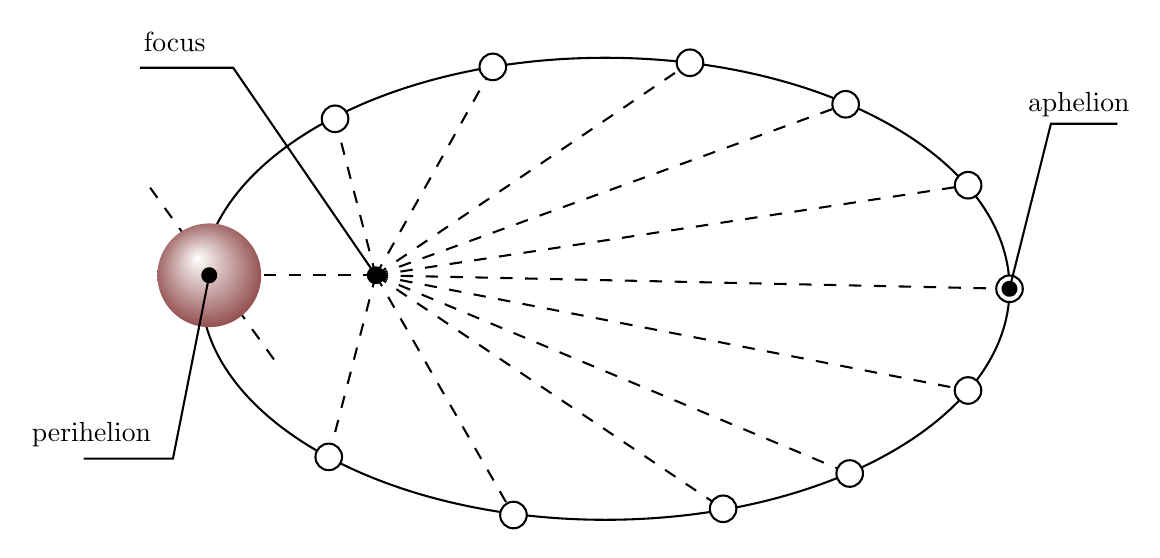
\begin{tikzpicture}[x=0.75pt,y=0.75pt,yscale=-1,xscale=1]
		%uncomment if require: \path (0,1046); %set diagram left start at 0, and has height of 1046
		
		% Gradient Info
  
		\tikzset {_937blvzl3/.code = {\pgfsetadditionalshadetransform{ \pgftransformshift{\pgfpoint{89.1 bp } { -128.7 bp }  }  \pgftransformscale{1.32 }  }}}
		\pgfdeclareradialshading{_lo8d8s0ax}{\pgfpoint{-72bp}{104bp}}{rgb(0bp)=(1,1,1);
		rgb(0bp)=(1,1,1);
		rgb(25bp)=(0.48,0.15,0.15);
		rgb(400bp)=(0.48,0.15,0.15)}
		
		%Straight Lines [id:da7557302287256482] 
		\draw  [dash pattern={on 4.5pt off 4.5pt}]  (200.2,160.8) -- (505.55,167.3) ;
		%Straight Lines [id:da17311054905098788] 
		\draw  [dash pattern={on 4.5pt off 4.5pt}]  (200.2,160.8) -- (180.6,85.4) ;
		%Straight Lines [id:da7142340941166672] 
		\draw  [dash pattern={on 4.5pt off 4.5pt}]  (200.2,160.8) -- (256.6,60.4) ;
		%Straight Lines [id:da43553145089569467] 
		\draw  [dash pattern={on 4.5pt off 4.5pt}]  (200.2,160.8) -- (351.6,58.4) ;
		%Straight Lines [id:da4705555466766196] 
		\draw  [dash pattern={on 4.5pt off 4.5pt}]  (200.2,160.8) -- (426.6,78.4) ;
		%Straight Lines [id:da2954858545726562] 
		\draw  [dash pattern={on 4.5pt off 4.5pt}]  (200.2,160.8) -- (485.6,117.4) ;
		%Straight Lines [id:da9685439997375054] 
		\draw  [dash pattern={on 4.5pt off 4.5pt}]  (200.2,160.8) -- (485.55,216.3) ;
		%Straight Lines [id:da951666184427381] 
		\draw  [dash pattern={on 4.5pt off 4.5pt}]  (200.2,160.8) -- (428.55,256.3) ;
		%Straight Lines [id:da0517486468656132] 
		\draw  [dash pattern={on 4.5pt off 4.5pt}]  (200.2,160.8) -- (367.55,273.3) ;
		%Straight Lines [id:da25254617556541903] 
		\draw  [dash pattern={on 4.5pt off 4.5pt}]  (200.2,160.8) -- (266.55,276.3) ;
		%Straight Lines [id:da20746323149422108] 
		\draw  [dash pattern={on 4.5pt off 4.5pt}]  (200.2,160.8) -- (177.55,248.3) ;
		%Straight Lines [id:da1256605474878636] 
		\draw  [dash pattern={on 4.5pt off 4.5pt}]  (91.5,118.6) -- (153.5,204.6) ;
		%Straight Lines [id:da24439792905703484] 
		\draw  [dash pattern={on 4.5pt off 4.5pt}]  (200.2,160.8) -- (120,160.8) ;
		%Shape: Ellipse [id:dp1294380217598965] 
		\draw   (116,167.3) .. controls (116,105.83) and (203.2,56) .. (310.77,56) .. controls (418.35,56) and (505.55,105.83) .. (505.55,167.3) .. controls (505.55,228.77) and (418.35,278.6) .. (310.77,278.6) .. controls (203.2,278.6) and (116,228.77) .. (116,167.3) -- cycle ;
		%Shape: Circle [id:dp706762933949838] 
		\draw  [draw opacity=0][shading=_lo8d8s0ax,_937blvzl3] (95,160.8) .. controls (95,146.99) and (106.19,135.8) .. (120,135.8) .. controls (133.81,135.8) and (145,146.99) .. (145,160.8) .. controls (145,174.61) and (133.81,185.8) .. (120,185.8) .. controls (106.19,185.8) and (95,174.61) .. (95,160.8) -- cycle ;
		%Shape: Circle [id:dp593978239510953] 
		\draw  [fill={rgb, 255:red, 0; green, 0; blue, 0 }  ,fill opacity=1 ] (196.4,160.8) .. controls (196.4,158.7) and (198.1,157) .. (200.2,157) .. controls (202.3,157) and (204,158.7) .. (204,160.8) .. controls (204,162.9) and (202.3,164.6) .. (200.2,164.6) .. controls (198.1,164.6) and (196.4,162.9) .. (196.4,160.8) -- cycle ;
		%Straight Lines [id:da21819223043716263] 
		\draw    (59.5,249.1) -- (102.5,249.1) -- (120,160.8) ;
		\draw [shift={(120,160.8)}, rotate = 281.21] [color={rgb, 255:red, 0; green, 0; blue, 0 }  ][fill={rgb, 255:red, 0; green, 0; blue, 0 }  ][line width=0.75]      (0, 0) circle [x radius= 3.35, y radius= 3.35]   ;
		%Straight Lines [id:da7042636298957099] 
		\draw    (86.5,60.8) -- (131.5,60.8) -- (200.2,160.8) ;
		\draw [shift={(200.2,160.8)}, rotate = 55.51] [color={rgb, 255:red, 0; green, 0; blue, 0 }  ][fill={rgb, 255:red, 0; green, 0; blue, 0 }  ][line width=0.75]      (0, 0) circle [x radius= 3.35, y radius= 3.35]   ;
		%Shape: Circle [id:dp3214966801594772] 
		\draw  [fill={rgb, 255:red, 255; green, 255; blue, 255 }  ,fill opacity=1 ] (174.2,85.4) .. controls (174.2,81.87) and (177.07,79) .. (180.6,79) .. controls (184.13,79) and (187,81.87) .. (187,85.4) .. controls (187,88.93) and (184.13,91.8) .. (180.6,91.8) .. controls (177.07,91.8) and (174.2,88.93) .. (174.2,85.4) -- cycle ;
		%Shape: Circle [id:dp08600326054575103] 
		\draw  [fill={rgb, 255:red, 255; green, 255; blue, 255 }  ,fill opacity=1 ] (250.2,60.4) .. controls (250.2,56.87) and (253.07,54) .. (256.6,54) .. controls (260.13,54) and (263,56.87) .. (263,60.4) .. controls (263,63.93) and (260.13,66.8) .. (256.6,66.8) .. controls (253.07,66.8) and (250.2,63.93) .. (250.2,60.4) -- cycle ;
		%Shape: Circle [id:dp3088903366513611] 
		\draw  [fill={rgb, 255:red, 255; green, 255; blue, 255 }  ,fill opacity=1 ] (345.2,58.4) .. controls (345.2,54.87) and (348.07,52) .. (351.6,52) .. controls (355.13,52) and (358,54.87) .. (358,58.4) .. controls (358,61.93) and (355.13,64.8) .. (351.6,64.8) .. controls (348.07,64.8) and (345.2,61.93) .. (345.2,58.4) -- cycle ;
		%Shape: Circle [id:dp09151589585870035] 
		\draw  [fill={rgb, 255:red, 255; green, 255; blue, 255 }  ,fill opacity=1 ] (420.2,78.4) .. controls (420.2,74.87) and (423.07,72) .. (426.6,72) .. controls (430.13,72) and (433,74.87) .. (433,78.4) .. controls (433,81.93) and (430.13,84.8) .. (426.6,84.8) .. controls (423.07,84.8) and (420.2,81.93) .. (420.2,78.4) -- cycle ;
		%Shape: Circle [id:dp2060371517763333] 
		\draw  [fill={rgb, 255:red, 255; green, 255; blue, 255 }  ,fill opacity=1 ] (479.2,117.4) .. controls (479.2,113.87) and (482.07,111) .. (485.6,111) .. controls (489.13,111) and (492,113.87) .. (492,117.4) .. controls (492,120.93) and (489.13,123.8) .. (485.6,123.8) .. controls (482.07,123.8) and (479.2,120.93) .. (479.2,117.4) -- cycle ;
		%Shape: Circle [id:dp7532714555982252] 
		\draw  [fill={rgb, 255:red, 255; green, 255; blue, 255 }  ,fill opacity=1 ] (499.15,167.3) .. controls (499.15,163.77) and (502.02,160.9) .. (505.55,160.9) .. controls (509.08,160.9) and (511.95,163.77) .. (511.95,167.3) .. controls (511.95,170.83) and (509.08,173.7) .. (505.55,173.7) .. controls (502.02,173.7) and (499.15,170.83) .. (499.15,167.3) -- cycle ;
		%Shape: Circle [id:dp10889227179352501] 
		\draw  [fill={rgb, 255:red, 255; green, 255; blue, 255 }  ,fill opacity=1 ] (479.15,216.3) .. controls (479.15,212.77) and (482.02,209.9) .. (485.55,209.9) .. controls (489.08,209.9) and (491.95,212.77) .. (491.95,216.3) .. controls (491.95,219.83) and (489.08,222.7) .. (485.55,222.7) .. controls (482.02,222.7) and (479.15,219.83) .. (479.15,216.3) -- cycle ;
		%Shape: Circle [id:dp6817046522714567] 
		\draw  [fill={rgb, 255:red, 255; green, 255; blue, 255 }  ,fill opacity=1 ] (422.15,256.3) .. controls (422.15,252.77) and (425.02,249.9) .. (428.55,249.9) .. controls (432.08,249.9) and (434.95,252.77) .. (434.95,256.3) .. controls (434.95,259.83) and (432.08,262.7) .. (428.55,262.7) .. controls (425.02,262.7) and (422.15,259.83) .. (422.15,256.3) -- cycle ;
		%Shape: Circle [id:dp9075427108041252] 
		\draw  [fill={rgb, 255:red, 255; green, 255; blue, 255 }  ,fill opacity=1 ] (361.15,273.3) .. controls (361.15,269.77) and (364.02,266.9) .. (367.55,266.9) .. controls (371.08,266.9) and (373.95,269.77) .. (373.95,273.3) .. controls (373.95,276.83) and (371.08,279.7) .. (367.55,279.7) .. controls (364.02,279.7) and (361.15,276.83) .. (361.15,273.3) -- cycle ;
		%Shape: Circle [id:dp7106772946108184] 
		\draw  [fill={rgb, 255:red, 255; green, 255; blue, 255 }  ,fill opacity=1 ] (260.15,276.3) .. controls (260.15,272.77) and (263.02,269.9) .. (266.55,269.9) .. controls (270.08,269.9) and (272.95,272.77) .. (272.95,276.3) .. controls (272.95,279.83) and (270.08,282.7) .. (266.55,282.7) .. controls (263.02,282.7) and (260.15,279.83) .. (260.15,276.3) -- cycle ;
		%Shape: Circle [id:dp14308990638741892] 
		\draw  [fill={rgb, 255:red, 255; green, 255; blue, 255 }  ,fill opacity=1 ] (171.15,248.3) .. controls (171.15,244.77) and (174.02,241.9) .. (177.55,241.9) .. controls (181.08,241.9) and (183.95,244.77) .. (183.95,248.3) .. controls (183.95,251.83) and (181.08,254.7) .. (177.55,254.7) .. controls (174.02,254.7) and (171.15,251.83) .. (171.15,248.3) -- cycle ;
		%Straight Lines [id:da3140788132332215] 
		\draw    (557.5,87.8) -- (525.5,87.8) -- (505.55,167.3) ;
		\draw [shift={(505.55,167.3)}, rotate = 104.09] [color={rgb, 255:red, 0; green, 0; blue, 0 }  ][fill={rgb, 255:red, 0; green, 0; blue, 0 }  ][line width=0.75]      (0, 0) circle [x radius= 3.35, y radius= 3.35]   ;
		
		% Text Node
		\draw (33,230) node [anchor=north west][inner sep=0.75pt]   [align=left] {perihelion};
		% Text Node
		\draw (87,42) node [anchor=north west][inner sep=0.75pt]   [align=left] {focus};
		% Text Node
		\draw (513,71) node [anchor=north west][inner sep=0.75pt]   [align=left] {aphelion};
		
		\end{tikzpicture}
		\vspace*{3mm}
		\caption{Representation of surfaces conservation} 
	\end{figure}
	This is true for the Earth for example. Indeed, this latter is closer to the Sun in winter (for northern hemisphere) and then has a trajectory speed slightly higher than in summer; the travel time is therefore lower (winter has fewer days than the other seasons).
	
	The above figure is often represented in textbooks as:
	\begin{figure}[H]
		\centering
		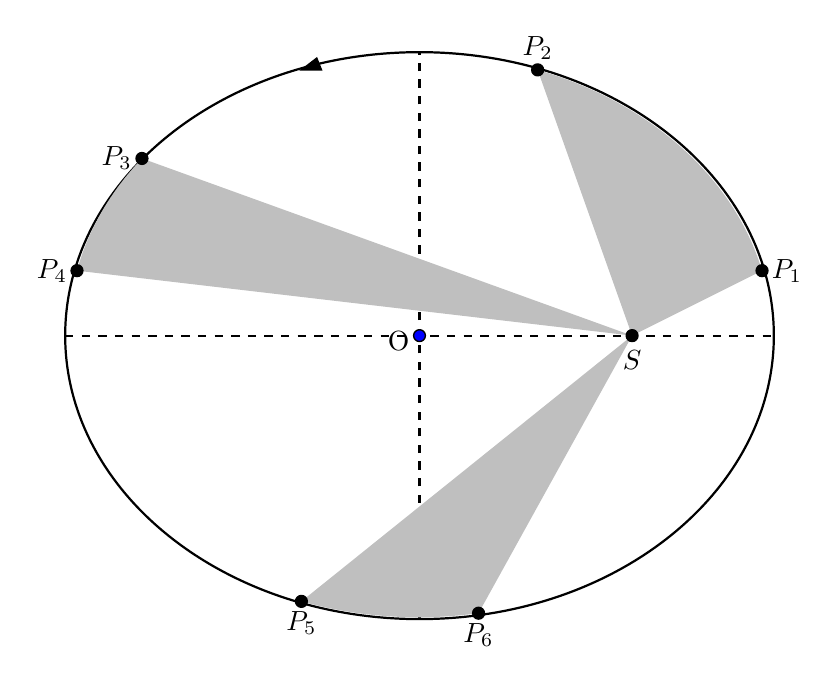
\begin{tikzpicture}[scale=1.5]
		\draw[black, thick] (0,0) ellipse (3 and 2.4);
		\draw[dashed] (-3,0) -- (3,0); 
		\draw[dashed] (0,-2.4) -- (0, 2.4);
		
		
		\pgfsetfillcolor{gray!50}
		\pgfsetlinewidth{0.5pt}
		
		\pgfpathmoveto{\pgfpoint{1.8cm}{0cm}}
		\pgfpathlineto{\pgfpoint{1cm}{2.25cm}}
		\pgfpatharcto{3cm}{2.4cm}{0}{0}{0}{\pgfpoint{2.9cm}{0.55cm}}
		\pgfpathlineto{\pgfpoint{1.8cm}{0cm}}
		\pgfpathclose
		\pgfusepath{fill}
		
		\pgfpathmoveto{\pgfpoint{1.8cm}{0cm}}
		\pgfpathlineto{\pgfpoint{-2.35cm}{1.5cm}}
		\pgfpatharcto{3cm}{2.4cm}{0}{0}{-1}{\pgfpoint{-2.9cm}{0.55cm}}
		\pgfpathlineto{\pgfpoint{1.8cm}{0cm}}
		\pgfpathclose
		\pgfusepath{fill}
		
		\pgfpathmoveto{\pgfpoint{1.8cm}{0cm}}
		\pgfpathlineto{\pgfpoint{-1cm}{-2.25cm}}
		\pgfpatharcto{3cm}{2.4cm}{0}{0}{-1}{\pgfpoint{0.5cm}{-2.35cm}}
		\pgfpathlineto{\pgfpoint{1.8cm}{0cm}}
		\pgfpathclose
		\pgfusepath{fill}
		
		\draw[fill=blue] (0.0,0) circle(0.5mm) node[below=2,left=0.1] {O};
		\draw[fill=black] (1.8,0) circle(0.5mm) node[below=2] {$S$};
		\draw[fill=black] (2.9, 0.55) circle(0.5mm) node[right] {$P_{1}$};
		\draw[fill=black] (1, 2.25) circle(0.5mm) node[above] {$P_{2}$};
		\draw[fill=black] (-2.35, 1.5) circle(0.5mm) node[left=0.1] {$P_{3}$};
		\draw[fill=black] (-2.9, 0.55) circle(0.5mm) node[left] {$P_{4}$};
		\draw[fill=black] (-1, -2.25) circle(0.5mm) node[below] {$P_{5}$};
		\draw[fill=black] (0.5, -2.35) circle(0.5mm) node[below] {$P_{6}$};
		\draw[fill=black] (-1,2.25) -- (-0.87,2.35) -- (-0.83,2.25) -- cycle;
		\end{tikzpicture}
	\end{figure}
	
	\paragraph{Time of flight}\mbox{}\\\\
	We propose now to apply the second Kepler's law to determine the time $t$ from the passage to the perihelion as a function of the "\NewTerm{eccentric anomaly}\index{eccentric anomaly}" $\varphi$ in the case of an elliptic orbit  (thus special case!) using its two foci (one of them being assimilable for example to the position of the Sun) and the origin of the "\NewTerm{auxiliary circle}\index{auxiliary circle}" (also named "\NewTerm{apsidal circle}\index{apsidal circle}"):
	\begin{figure}[H]
		\centering
		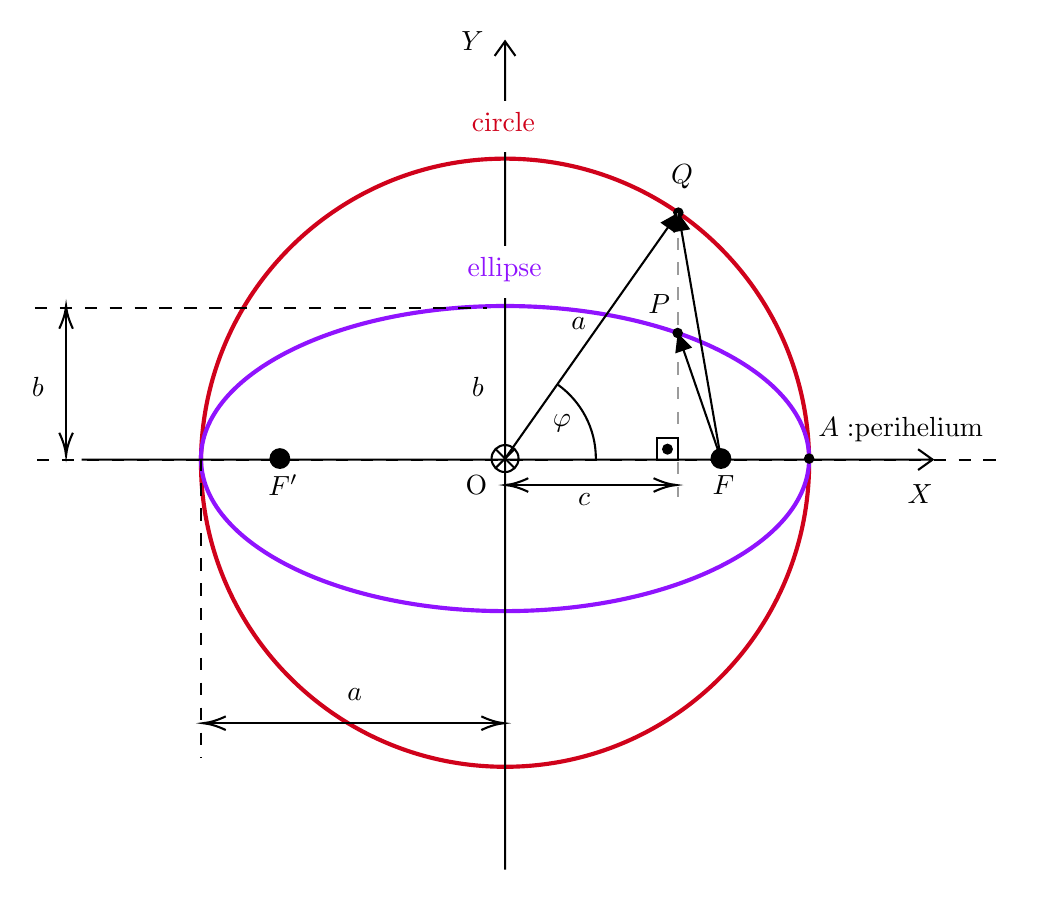
\begin{tikzpicture}[x=0.75pt,y=0.75pt,yscale=-1,xscale=1]
		%uncomment if require: \path (0,954); %set diagram left start at 0, and has height of 954
		
		%Shape: Circle [id:dp9842774993674039] 
		\draw  [color={rgb, 255:red, 208; green, 2; blue, 27 }  ,draw opacity=1 ][line width=1.5]  (169,233.5) .. controls (169,152.59) and (234.59,87) .. (315.5,87) .. controls (396.41,87) and (462,152.59) .. (462,233.5) .. controls (462,314.41) and (396.41,380) .. (315.5,380) .. controls (234.59,380) and (169,314.41) .. (169,233.5) -- cycle ;
		%Shape: Ellipse [id:dp3444633374110706] 
		\draw  [color={rgb, 255:red, 144; green, 19; blue, 254 }  ,draw opacity=1 ][line width=1.5]  (169,231.5) .. controls (169,190.91) and (234.59,158) .. (315.5,158) .. controls (396.41,158) and (462,190.91) .. (462,231.5) .. controls (462,272.09) and (396.41,305) .. (315.5,305) .. controls (234.59,305) and (169,272.09) .. (169,231.5) -- cycle ;
		%Straight Lines [id:da336525086630894] 
		\draw  [dash pattern={on 4.5pt off 4.5pt}]  (90,232) -- (558,232) ;
		%Straight Lines [id:da9393308570267538] 
		\draw  [dash pattern={on 4.5pt off 4.5pt}]  (89,159) -- (307,159) ;
		%Straight Lines [id:da9825715721660542] 
		\draw  [dash pattern={on 4.5pt off 4.5pt}]  (315.5,231.5) -- (315.5,347) ;
		%Shape: Axis 2D [id:dp355765610003105] 
		\draw  (111.5,232) -- (521.5,232)(315.5,30.5) -- (315.5,429.5) (514.5,227) -- (521.5,232) -- (514.5,237) (310.5,37.5) -- (315.5,30.5) -- (320.5,37.5)  ;
		%Straight Lines [id:da7452331759875623] 
		\draw    (104,160) -- (104,228) ;
		\draw [shift={(104,230)}, rotate = 270] [color={rgb, 255:red, 0; green, 0; blue, 0 }  ][line width=0.75]    (10.93,-3.29) .. controls (6.95,-1.4) and (3.31,-0.3) .. (0,0) .. controls (3.31,0.3) and (6.95,1.4) .. (10.93,3.29)   ;
		\draw [shift={(104,158)}, rotate = 90] [color={rgb, 255:red, 0; green, 0; blue, 0 }  ][line width=0.75]    (10.93,-3.29) .. controls (6.95,-1.4) and (3.31,-0.3) .. (0,0) .. controls (3.31,0.3) and (6.95,1.4) .. (10.93,3.29)   ;
		%Flowchart: Summing Junction [id:dp5692235084362796] 
		\draw   (309,231.5) .. controls (309,227.91) and (311.91,225) .. (315.5,225) .. controls (319.09,225) and (322,227.91) .. (322,231.5) .. controls (322,235.09) and (319.09,238) .. (315.5,238) .. controls (311.91,238) and (309,235.09) .. (309,231.5) -- cycle ; \draw   (310.9,226.9) -- (320.1,236.1) ; \draw   (320.1,226.9) -- (310.9,236.1) ;
		%Straight Lines [id:da3364773022710683] 
		\draw  [dash pattern={on 4.5pt off 4.5pt}]  (169,231.5) -- (169,376) ;
		%Straight Lines [id:da5912510104688169] 
		\draw    (313,359) -- (172,359) ;
		\draw [shift={(170,359)}, rotate = 360] [color={rgb, 255:red, 0; green, 0; blue, 0 }  ][line width=0.75]    (10.93,-3.29) .. controls (6.95,-1.4) and (3.31,-0.3) .. (0,0) .. controls (3.31,0.3) and (6.95,1.4) .. (10.93,3.29)   ;
		\draw [shift={(315,359)}, rotate = 180] [color={rgb, 255:red, 0; green, 0; blue, 0 }  ][line width=0.75]    (10.93,-3.29) .. controls (6.95,-1.4) and (3.31,-0.3) .. (0,0) .. controls (3.31,0.3) and (6.95,1.4) .. (10.93,3.29)   ;
		%Shape: Circle [id:dp7489500132298774] 
		\draw  [fill={rgb, 255:red, 0; green, 0; blue, 0 }  ,fill opacity=1 ] (415,231.5) .. controls (415,229.01) and (417.01,227) .. (419.5,227) .. controls (421.99,227) and (424,229.01) .. (424,231.5) .. controls (424,233.99) and (421.99,236) .. (419.5,236) .. controls (417.01,236) and (415,233.99) .. (415,231.5) -- cycle ;
		%Straight Lines [id:da7725409789202062] 
		\draw    (396,244.25) -- (317.75,244.25) ;
		\draw [shift={(315.75,244.25)}, rotate = 360] [color={rgb, 255:red, 0; green, 0; blue, 0 }  ][line width=0.75]    (10.93,-3.29) .. controls (6.95,-1.4) and (3.31,-0.3) .. (0,0) .. controls (3.31,0.3) and (6.95,1.4) .. (10.93,3.29)   ;
		\draw [shift={(398,244.25)}, rotate = 180] [color={rgb, 255:red, 0; green, 0; blue, 0 }  ][line width=0.75]    (10.93,-3.29) .. controls (6.95,-1.4) and (3.31,-0.3) .. (0,0) .. controls (3.31,0.3) and (6.95,1.4) .. (10.93,3.29)   ;
		%Straight Lines [id:da479175103529607] 
		\draw    (315.5,231.5) -- (397.27,115.45) ;
		\draw [shift={(399,113)}, rotate = 125.17] [fill={rgb, 255:red, 0; green, 0; blue, 0 }  ][line width=0.08]  [draw opacity=0] (8.93,-4.29) -- (0,0) -- (8.93,4.29) -- cycle    ;
		%Shape: Circle [id:dp5400237493038627] 
		\draw  [fill={rgb, 255:red, 0; green, 0; blue, 0 }  ,fill opacity=1 ] (397,113) .. controls (397,111.9) and (397.9,111) .. (399,111) .. controls (400.1,111) and (401,111.9) .. (401,113) .. controls (401,114.1) and (400.1,115) .. (399,115) .. controls (397.9,115) and (397,114.1) .. (397,113) -- cycle ;
		%Shape: Circle [id:dp8221156751740817] 
		\draw  [fill={rgb, 255:red, 0; green, 0; blue, 0 }  ,fill opacity=1 ] (396.67,171) .. controls (396.67,169.9) and (397.56,169) .. (398.67,169) .. controls (399.77,169) and (400.67,169.9) .. (400.67,171) .. controls (400.67,172.1) and (399.77,173) .. (398.67,173) .. controls (397.56,173) and (396.67,172.1) .. (396.67,171) -- cycle ;
		%Straight Lines [id:da06315534492599473] 
		\draw [color={rgb, 255:red, 155; green, 155; blue, 155 }  ,draw opacity=1 ] [dash pattern={on 4.5pt off 4.5pt}]  (399,113) -- (399,250) ;
		%Straight Lines [id:da5913936150459307] 
		\draw    (419.5,231.5) -- (399.51,115.96) ;
		\draw [shift={(399,113)}, rotate = 80.19] [fill={rgb, 255:red, 0; green, 0; blue, 0 }  ][line width=0.08]  [draw opacity=0] (8.93,-4.29) -- (0,0) -- (8.93,4.29) -- cycle    ;
		%Shape: Arc [id:dp7848199604482449] 
		\draw  [draw opacity=0] (341.03,195.96) .. controls (352.06,203.91) and (359.25,216.86) .. (359.25,231.5) .. controls (359.25,231.67) and (359.25,231.83) .. (359.25,232) -- (315.5,231.5) -- cycle ; \draw   (341.03,195.96) .. controls (352.06,203.91) and (359.25,216.86) .. (359.25,231.5) .. controls (359.25,231.67) and (359.25,231.83) .. (359.25,232) ;  
		%Shape: Rectangle [id:dp5589260665521327] 
		\draw   (388.5,221.61) -- (399,221.61) -- (399,232.34) -- (388.5,232.34) -- cycle ;
		%Shape: Ellipse [id:dp9589868490730598] 
		\draw  [fill={rgb, 255:red, 0; green, 0; blue, 0 }  ,fill opacity=1 ] (391.65,226.97) .. controls (391.65,225.79) and (392.59,224.83) .. (393.75,224.83) .. controls (394.91,224.83) and (395.85,225.79) .. (395.85,226.97) .. controls (395.85,228.16) and (394.91,229.12) .. (393.75,229.12) .. controls (392.59,229.12) and (391.65,228.16) .. (391.65,226.97) -- cycle ;
		
		%Shape: Circle [id:dp7562646903874228] 
		\draw  [fill={rgb, 255:red, 0; green, 0; blue, 0 }  ,fill opacity=1 ] (460,231.5) .. controls (460,230.4) and (460.9,229.5) .. (462,229.5) .. controls (463.1,229.5) and (464,230.4) .. (464,231.5) .. controls (464,232.6) and (463.1,233.5) .. (462,233.5) .. controls (460.9,233.5) and (460,232.6) .. (460,231.5) -- cycle ;
		%Shape: Circle [id:dp6079972505093689] 
		\draw  [fill={rgb, 255:red, 0; green, 0; blue, 0 }  ,fill opacity=1 ] (202.5,231.5) .. controls (202.5,229.01) and (204.51,227) .. (207,227) .. controls (209.49,227) and (211.5,229.01) .. (211.5,231.5) .. controls (211.5,233.99) and (209.49,236) .. (207,236) .. controls (204.51,236) and (202.5,233.99) .. (202.5,231.5) -- cycle ;
		%Straight Lines [id:da18251193132842203] 
		\draw    (419.5,231.5) -- (399.64,173.84) ;
		\draw [shift={(398.67,171)}, rotate = 71] [fill={rgb, 255:red, 0; green, 0; blue, 0 }  ][line width=0.08]  [draw opacity=0] (8.93,-4.29) -- (0,0) -- (8.93,4.29) -- cycle    ;
		
		% Text Node
		\draw (508,242.4) node [anchor=north west][inner sep=0.75pt]    {$X$};
		% Text Node
		\draw (293,24.4) node [anchor=north west][inner sep=0.75pt]    {$Y$};
		% Text Node
		\draw (298,190.9) node [anchor=north west][inner sep=0.75pt]    {$b$};
		% Text Node
		\draw (86,190.9) node [anchor=north west][inner sep=0.75pt]    {$b$};
		% Text Node
		\draw (295,238) node [anchor=north west][inner sep=0.75pt]   [align=left] {O};
		% Text Node
		\draw (238,341) node [anchor=north west][inner sep=0.75pt]    {$a$};
		% Text Node
		\draw (414,238) node [anchor=north west][inner sep=0.75pt]    {$F$};
		% Text Node
		\draw (349.25,247) node [anchor=north west][inner sep=0.75pt]    {$c$};
		% Text Node
		\draw (394,88.4) node [anchor=north west][inner sep=0.75pt]    {$Q$};
		% Text Node
		\draw (346,162) node [anchor=north west][inner sep=0.75pt]    {$a$};
		% Text Node
		\draw  [draw opacity=0][fill={rgb, 255:red, 255; green, 255; blue, 255 }  ,fill opacity=1 ]  (295,59) -- (338,59) -- (338,84) -- (295,84) -- cycle  ;
		\draw (298,63) node [anchor=north west][inner sep=0.75pt]  [color={rgb, 255:red, 208; green, 2; blue, 27 }  ,opacity=1 ] [align=left] {circle};
		% Text Node
		\draw  [draw opacity=0][fill={rgb, 255:red, 255; green, 255; blue, 255 }  ,fill opacity=1 ]  (293,129) -- (344,129) -- (344,154) -- (293,154) -- cycle  ;
		\draw (296,133) node [anchor=north west][inner sep=0.75pt]  [color={rgb, 255:red, 144; green, 19; blue, 254 }  ,opacity=1 ] [align=left] {ellipse};
		% Text Node
		\draw (337,209) node [anchor=north west][inner sep=0.75pt]    {$\varphi $};
		% Text Node
		\draw (200,238) node [anchor=north west][inner sep=0.75pt]    {$F'$};
		% Text Node
		\draw (465,210) node [anchor=north west][inner sep=0.75pt]   [align=left] {$\displaystyle A:$perihelium};
		% Text Node
		\draw (383,151.07) node [anchor=north west][inner sep=0.75pt]    {$P$};
		\end{tikzpicture}
		\vspace*{3mm}
		\caption{Schema for the study of eccentric anomaly angle}
	\end{figure}
	To determine the time $t$ between the passage at the perihelion $A$ and the point $P$ of a body following the trajectory of the ellipse of surface $\pi a b$ (see the section Geometric Shapes at page \pageref{surface of ellipse} for the proof of the calculation of the surface of the ellipse) in function of the eccentric anomaly $\varphi$, we will use the areas law just proved earlier above (second Kepler's law) that gives us the right to write:
	
	But, the surface of the ellipse is an affine transformation of the surface of the auxiliary circle such that:
	
 	We have then:
	
 	If $\varphi$ is, as it should, expressed in radians, we have of course:
	
 	Therefore:
	
 	For $S_{F\text{O}Q}$, we have $\overline{F\text{O}}=a$ therefore equal to the radius of the auxiliary circle. The surface of the triangle $S_{F\text{O}Q}$, knowing its height given by $h=a\sin(\varphi)$ is then obtained by:
	
	Therefore we have:
	
	But, by definition of the eccentricity (\SeeChapter{see section Analytical Geometry page \pageref{eccentricity}}), we can write:
	
	Finally, we have:
	
	Therefore:
	
 	where the angle taken at the center of the ellipse is for recall named the "eccentric anomaly".

	\textbf{Definition (\#\thesection.\mydef):} In the description of the Keplerian orbit of a celestial object, the "\NewTerm{eccentric anomaly}\index{eccentric anomaly}" is the angle between the direction of the periapse and the current position of an object in its orbit, projected on the circle extinct perpendicular to the major axis of the ellipse

	What would interest us now would be to find a relation of passage between this eccentric anomaly and the angle named "\NewTerm{true anomaly}\index{true anomaly}" $\theta$ as sometimes it is often more advantageous to use this last angle.

	For a relation between the eccentric anomaly $\varphi$ and the true anomaly $\theta$, we will reuse our above schema but modified a bit:
	\begin{figure}[H]
		\centering
		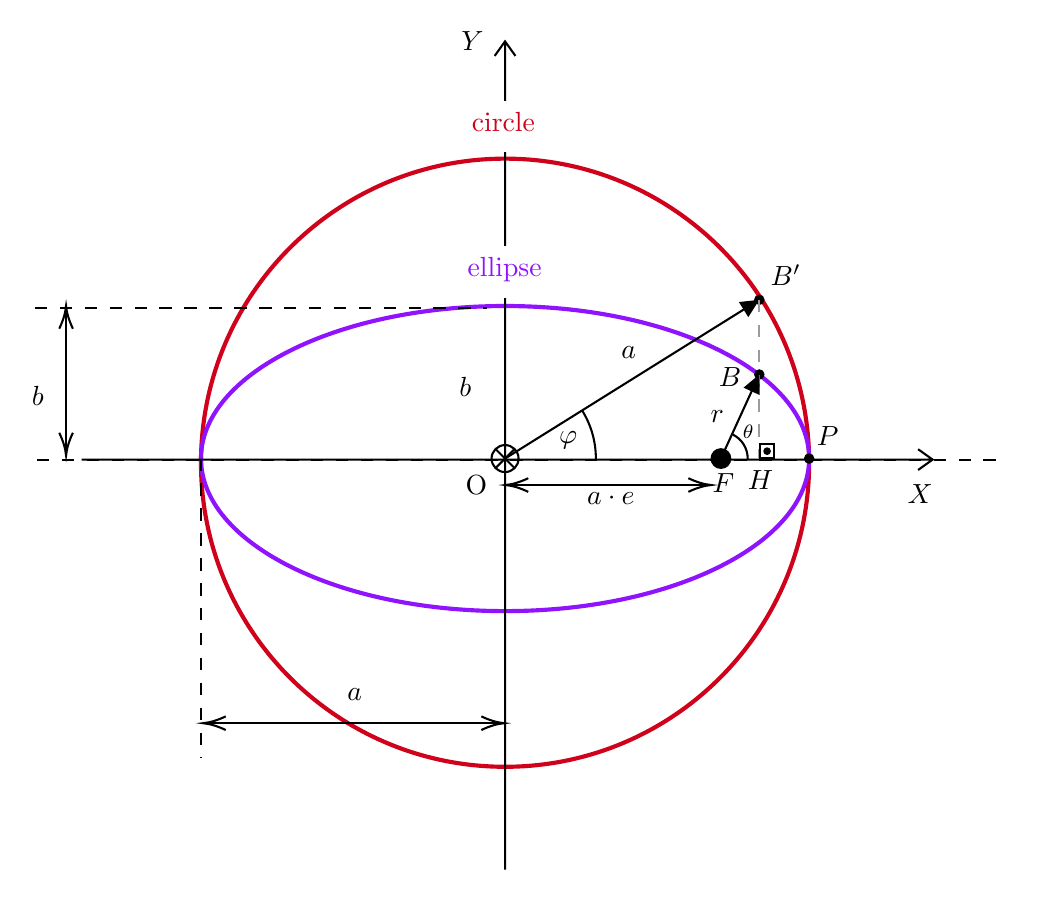
\begin{tikzpicture}[x=0.75pt,y=0.75pt,yscale=-1,xscale=1]
		%uncomment if require: \path (0,954); %set diagram left start at 0, and has height of 954
		
		%Shape: Circle [id:dp9842774993674039] 
		\draw  [color={rgb, 255:red, 208; green, 2; blue, 27 }  ,draw opacity=1 ][line width=1.5]  (169,233.5) .. controls (169,152.59) and (234.59,87) .. (315.5,87) .. controls (396.41,87) and (462,152.59) .. (462,233.5) .. controls (462,314.41) and (396.41,380) .. (315.5,380) .. controls (234.59,380) and (169,314.41) .. (169,233.5) -- cycle ;
		%Shape: Ellipse [id:dp3444633374110706] 
		\draw  [color={rgb, 255:red, 144; green, 19; blue, 254 }  ,draw opacity=1 ][line width=1.5]  (169,231.5) .. controls (169,190.91) and (234.59,158) .. (315.5,158) .. controls (396.41,158) and (462,190.91) .. (462,231.5) .. controls (462,272.09) and (396.41,305) .. (315.5,305) .. controls (234.59,305) and (169,272.09) .. (169,231.5) -- cycle ;
		%Straight Lines [id:da336525086630894] 
		\draw  [dash pattern={on 4.5pt off 4.5pt}]  (90,232) -- (558,232) ;
		%Straight Lines [id:da9393308570267538] 
		\draw  [dash pattern={on 4.5pt off 4.5pt}]  (89,159) -- (307,159) ;
		%Straight Lines [id:da9825715721660542] 
		\draw  [dash pattern={on 4.5pt off 4.5pt}]  (315.5,231.5) -- (315.5,347) ;
		%Shape: Axis 2D [id:dp355765610003105] 
		\draw  (111.5,232) -- (521.5,232)(315.5,30.5) -- (315.5,429.5) (514.5,227) -- (521.5,232) -- (514.5,237) (310.5,37.5) -- (315.5,30.5) -- (320.5,37.5)  ;
		%Straight Lines [id:da7452331759875623] 
		\draw    (104,160) -- (104,228) ;
		\draw [shift={(104,230)}, rotate = 270] [color={rgb, 255:red, 0; green, 0; blue, 0 }  ][line width=0.75]    (10.93,-3.29) .. controls (6.95,-1.4) and (3.31,-0.3) .. (0,0) .. controls (3.31,0.3) and (6.95,1.4) .. (10.93,3.29)   ;
		\draw [shift={(104,158)}, rotate = 90] [color={rgb, 255:red, 0; green, 0; blue, 0 }  ][line width=0.75]    (10.93,-3.29) .. controls (6.95,-1.4) and (3.31,-0.3) .. (0,0) .. controls (3.31,0.3) and (6.95,1.4) .. (10.93,3.29)   ;
		%Flowchart: Summing Junction [id:dp5692235084362796] 
		\draw   (309,231.5) .. controls (309,227.91) and (311.91,225) .. (315.5,225) .. controls (319.09,225) and (322,227.91) .. (322,231.5) .. controls (322,235.09) and (319.09,238) .. (315.5,238) .. controls (311.91,238) and (309,235.09) .. (309,231.5) -- cycle ; \draw   (310.9,226.9) -- (320.1,236.1) ; \draw   (320.1,226.9) -- (310.9,236.1) ;
		%Straight Lines [id:da3364773022710683] 
		\draw  [dash pattern={on 4.5pt off 4.5pt}]  (169,231.5) -- (169,376) ;
		%Straight Lines [id:da5912510104688169] 
		\draw    (313,359) -- (172,359) ;
		\draw [shift={(170,359)}, rotate = 360] [color={rgb, 255:red, 0; green, 0; blue, 0 }  ][line width=0.75]    (10.93,-3.29) .. controls (6.95,-1.4) and (3.31,-0.3) .. (0,0) .. controls (3.31,0.3) and (6.95,1.4) .. (10.93,3.29)   ;
		\draw [shift={(315,359)}, rotate = 180] [color={rgb, 255:red, 0; green, 0; blue, 0 }  ][line width=0.75]    (10.93,-3.29) .. controls (6.95,-1.4) and (3.31,-0.3) .. (0,0) .. controls (3.31,0.3) and (6.95,1.4) .. (10.93,3.29)   ;
		%Shape: Circle [id:dp7489500132298774] 
		\draw  [fill={rgb, 255:red, 0; green, 0; blue, 0 }  ,fill opacity=1 ] (415,231.5) .. controls (415,229.01) and (417.01,227) .. (419.5,227) .. controls (421.99,227) and (424,229.01) .. (424,231.5) .. controls (424,233.99) and (421.99,236) .. (419.5,236) .. controls (417.01,236) and (415,233.99) .. (415,231.5) -- cycle ;
		%Straight Lines [id:da7725409789202062] 
		\draw    (412.75,244.25) -- (317.75,244.25) ;
		\draw [shift={(315.75,244.25)}, rotate = 360] [color={rgb, 255:red, 0; green, 0; blue, 0 }  ][line width=0.75]    (10.93,-3.29) .. controls (6.95,-1.4) and (3.31,-0.3) .. (0,0) .. controls (3.31,0.3) and (6.95,1.4) .. (10.93,3.29)   ;
		\draw [shift={(414.75,244.25)}, rotate = 180] [color={rgb, 255:red, 0; green, 0; blue, 0 }  ][line width=0.75]    (10.93,-3.29) .. controls (6.95,-1.4) and (3.31,-0.3) .. (0,0) .. controls (3.31,0.3) and (6.95,1.4) .. (10.93,3.29)   ;
		%Straight Lines [id:da479175103529607] 
		\draw    (315.5,231.5) -- (435.46,156.59) ;
		\draw [shift={(438,155)}, rotate = 148.02] [fill={rgb, 255:red, 0; green, 0; blue, 0 }  ][line width=0.08]  [draw opacity=0] (8.93,-4.29) -- (0,0) -- (8.93,4.29) -- cycle    ;
		%Shape: Circle [id:dp5400237493038627] 
		\draw  [fill={rgb, 255:red, 0; green, 0; blue, 0 }  ,fill opacity=1 ] (436,155) .. controls (436,153.9) and (436.9,153) .. (438,153) .. controls (439.1,153) and (440,153.9) .. (440,155) .. controls (440,156.1) and (439.1,157) .. (438,157) .. controls (436.9,157) and (436,156.1) .. (436,155) -- cycle ;
		%Shape: Circle [id:dp8221156751740817] 
		\draw  [fill={rgb, 255:red, 0; green, 0; blue, 0 }  ,fill opacity=1 ] (436,191) .. controls (436,189.9) and (436.9,189) .. (438,189) .. controls (439.1,189) and (440,189.9) .. (440,191) .. controls (440,192.1) and (439.1,193) .. (438,193) .. controls (436.9,193) and (436,192.1) .. (436,191) -- cycle ;
		%Straight Lines [id:da06315534492599473] 
		\draw [color={rgb, 255:red, 155; green, 155; blue, 155 }  ,draw opacity=1 ] [dash pattern={on 4.5pt off 4.5pt}]  (438,155) -- (438,231.25) ;
		%Straight Lines [id:da5913936150459307] 
		\draw    (419.5,231.5) -- (436.75,193.73) ;
		\draw [shift={(438,191)}, rotate = 114.55] [fill={rgb, 255:red, 0; green, 0; blue, 0 }  ][line width=0.08]  [draw opacity=0] (8.93,-4.29) -- (0,0) -- (8.93,4.29) -- cycle    ;
		%Shape: Arc [id:dp7848199604482449] 
		\draw  [draw opacity=0] (352.51,208.16) .. controls (356.78,214.91) and (359.25,222.92) .. (359.25,231.5) .. controls (359.25,231.67) and (359.25,231.83) .. (359.25,232) -- (315.5,231.5) -- cycle ; \draw   (352.51,208.16) .. controls (356.78,214.91) and (359.25,222.92) .. (359.25,231.5) .. controls (359.25,231.67) and (359.25,231.83) .. (359.25,232) ;  
		%Shape: Rectangle [id:dp5589260665521327] 
		\draw   (438.5,224.61) -- (445,224.61) -- (445,231.25) -- (438.5,231.25) -- cycle ;
		%Shape: Ellipse [id:dp9589868490730598] 
		\draw  [fill={rgb, 255:red, 0; green, 0; blue, 0 }  ,fill opacity=1 ] (440.45,227.93) .. controls (440.45,227.2) and (441.03,226.6) .. (441.75,226.6) .. controls (442.47,226.6) and (443.05,227.2) .. (443.05,227.93) .. controls (443.05,228.66) and (442.47,229.26) .. (441.75,229.26) .. controls (441.03,229.26) and (440.45,228.66) .. (440.45,227.93) -- cycle ;
		
		%Shape: Arc [id:dp3992439662058318] 
		\draw  [draw opacity=0] (425.27,219.95) .. controls (429.5,222.07) and (432.41,226.45) .. (432.41,231.5) .. controls (432.41,231.75) and (432.4,232) .. (432.39,232.24) -- (419.5,231.5) -- cycle ; \draw   (425.27,219.95) .. controls (429.5,222.07) and (432.41,226.45) .. (432.41,231.5) .. controls (432.41,231.75) and (432.4,232) .. (432.39,232.24) ;  
		%Shape: Circle [id:dp7562646903874228] 
		\draw  [fill={rgb, 255:red, 0; green, 0; blue, 0 }  ,fill opacity=1 ] (460,231.5) .. controls (460,230.4) and (460.9,229.5) .. (462,229.5) .. controls (463.1,229.5) and (464,230.4) .. (464,231.5) .. controls (464,232.6) and (463.1,233.5) .. (462,233.5) .. controls (460.9,233.5) and (460,232.6) .. (460,231.5) -- cycle ;
		
		% Text Node
		\draw (508,242.4) node [anchor=north west][inner sep=0.75pt]    {$X$};
		% Text Node
		\draw (293,24.4) node [anchor=north west][inner sep=0.75pt]    {$Y$};
		% Text Node
		\draw (292,190.9) node [anchor=north west][inner sep=0.75pt]    {$b$};
		% Text Node
		\draw (86,195) node [anchor=north west][inner sep=0.75pt]    {$b$};
		% Text Node
		\draw (295,238) node [anchor=north west][inner sep=0.75pt]   [align=left] {O};
		% Text Node
		\draw (238,341) node [anchor=north west][inner sep=0.75pt]    {$a$};
		% Text Node
		\draw (464.25,214.65) node [anchor=north west][inner sep=0.75pt]    {$P$};
		% Text Node
		\draw (414,237.4) node [anchor=north west][inner sep=0.75pt]    {$F$};
		% Text Node
		\draw (353.5,246.4) node [anchor=north west][inner sep=0.75pt]    {$a\cdot e$};
		% Text Node
		\draw (442,136.4) node [anchor=north west][inner sep=0.75pt]    {$B'$};
		% Text Node
		\draw (417,186.4) node [anchor=north west][inner sep=0.75pt]    {$B$};
		% Text Node
		\draw (370,176) node [anchor=north west][inner sep=0.75pt]    {$a$};
		% Text Node
		\draw  [draw opacity=0][fill={rgb, 255:red, 255; green, 255; blue, 255 }  ,fill opacity=1 ]  (295,59) -- (338,59) -- (338,84) -- (295,84) -- cycle  ;
		\draw (298,63) node [anchor=north west][inner sep=0.75pt]  [color={rgb, 255:red, 208; green, 2; blue, 27 }  ,opacity=1 ] [align=left] {circle};
		% Text Node
		\draw  [draw opacity=0][fill={rgb, 255:red, 255; green, 255; blue, 255 }  ,fill opacity=1 ]  (293,129) -- (344,129) -- (344,154) -- (293,154) -- cycle  ;
		\draw (296,133) node [anchor=north west][inner sep=0.75pt]  [color={rgb, 255:red, 144; green, 19; blue, 254 }  ,opacity=1 ] [align=left] {ellipse};
		% Text Node
		\draw (431,235.9) node [anchor=north west][inner sep=0.75pt]    {$H$};
		% Text Node
		\draw (340,217) node [anchor=north west][inner sep=0.75pt]    {$\varphi $};
		% Text Node
		\draw (413,207) node [anchor=north west][inner sep=0.75pt]    {$r$};
		% Text Node
		\draw (428.5,213.9) node [anchor=north west][inner sep=0.75pt]  [font=\scriptsize]  {$\theta $};
		\end{tikzpicture}
		\vspace*{3mm}
		\caption{Schema for the study of true-eccentric anomaly angle relation}
	\end{figure}
	We have obviously the $4$ below relations which a deduce from the above figure:
	
	We then have already in a first time (relation which will be useful to us a little later):
	
 	We have also proved in the section of Analytical Geometry that (see page \pageref{parameter of the ellipse}):
	
	this relation being valid at any border point of the ellipse. Thus, we also have:
	
 	Which leads us to write:
	
	Ideally, we could get rid of the radius in the denominator. For this, we will use the fact that (relations that we have just proved earlier above):
	
	We have:
	
 	The terms to the left of the equality are simplified immediately:
	
	hence:
	
 	therefore:
	
	thus finally:
	
	Finally notice that in the special case of an elliptical orbit, we deduce thanks to the second Kepler's law (see the proof of the calculation of an area of an ellipse in the section Geometric Shapes page \pageref{ellipse}) the:
	
	\pagebreak
	\subsubsection{Third Kepler's Law (periods' law)}\label{third kepler law}
	The "\NewTerm{Kepler's third law}\index{Kepler's third law}", sometimes also named  "\NewTerm{Periods' law}\index{Periods' law}" or "\NewTerm{Kepler's harmonic law}\index{Kepler's harmonic law}", is stated as follow: The squares of the periods of revolution $T$ are proportional to the cube of the semi-major axes of the orbits $D$:
	
	The last ratio is then a constant in practice for all planets (in physics we also speak of "invariant") and the reason for this "harmony" was difficult to explain before Newton's theory.
	
	Again, we will see later that the status of "law" is no longer justified in our time as it is possible to prove that this relation, whose expression will be detailed, is in reality:
	
	and therefore we understand better when we see the term on the right why we had the previous constant ($m$ is the central body mass!).
	
	The last relation is more often written as following in the field of astronomy:
	
	where as we have seen in the section of Analytical Geometry, $a$ is the traditional notation for the semi major axis of ellipse. It is important to notice that whatever the magnitude of the semi minor axis,  if the semi major axis of multiple ellipses are identical, their periods (and therefore the corresponding total energy) will be identical.
	
	The most commonly used rearrangement of this last relation is obviously:
	
	Of course, Kepler did not immediately published his three laws in this provocative simplicity. Their current presentation order is also not the original one ... They are  in reality to find among  a profusion of physical speculations and reflections on world's harmony.
	
	\begin{tcolorbox}[title=Remark,arc=10pt,breakable,drop lifted shadow,
  skin=enhanced,
  skin first is subskin of={enhancedfirst}{arc=10pt,no shadow},
  skin middle is subskin of={enhancedmiddle}{arc=10pt,no shadow},
  skin last is subskin of={enhancedlast}{drop lifted shadow}]
	The Kepler's law are not limit to the gravitation force. They also apply for all acceleration (or force) of the type $1/r^2$. And this is also the case of the Coulomb's law (\SeeChapter{see section Electrostatics page \pageref{coulomb force}}). Kepler's law can therefore also be applied to an electron in orbit around a nucleus. The Wilson and Sommerfeld model (\SeeChapter{see section Quantum Corpuscular Physics page \pageref{wilson and sommerfled model}}) based also on Kepler's law gives also elliptic trajectories for electrons!
	\end{tcolorbox}	
	Here is an high definition image (you can zoom in a lot!) with some celestial bodies of the solar system, and for many of them, their orbital period $T$ and their distance $a$ to their main attractor:
	\begin{figure}[H]
		\centering
		\includegraphics[width=1.0\textwidth]{img/cosmology/bodies_of_the_solar_system.jpg}
		\caption[Some celestial bodies of our solar system]{Some celestial bodies of our solar system (author: Antonio Ciccolella)}
	\end{figure}
	We also recommend the reader to carefully look to the orbits structures schematized on the above figure as it will be useful for a critical thinking of the Newton Quantum Gravity model that we will introduce later (page \pageref{newton quantum gravity}).
	
	An interesting complementary image is to put side by side some well known planets and dwarf planets by respecting the proportions:
	\begin{figure}[H]
		\centering
		\includegraphics[width=1.0\textwidth]{img/cosmology/25_solar_system_objects_smaller_than_Earth.jpg}
		\caption[Side by side planets and dwarf planets]{Side by side planets and dwarf planets (source: ?)}
	\end{figure}
	For information, the rotation of Earth's on itself slows down at the day we write these lines of approximately $2.3$ milliseconds per century. That means $1$ hour every $180$ millions years. Each year the Earth's orbit speed around the Sun also slows down of approximately $3$ nanometers-per-second. Using Kepler's law, that means that the Earth goes further away from the Sun of $3$ micrometers per $1$ billion year......!!!!
	
	The three Kepler's law can then be summarized by the following small figure:
	\begin{figure}[H]
		\centering
		\begin{tikzpicture}[x=0.75pt,y=0.75pt,yscale=-1,xscale=1]
		%uncomment if require: \path (0,896); %set diagram left start at 0, and has height of 896
		
		% Gradient Info
	  
		\tikzset {_vzj7oi4gl/.code = {\pgfsetadditionalshadetransform{ \pgftransformshift{\pgfpoint{0 bp } { 0 bp }  }  \pgftransformscale{1 }  }}}
		\pgfdeclareradialshading{_n84vpl5lh}{\pgfpoint{0bp}{0bp}}{rgb(0bp)=(1,1,1);
		rgb(0bp)=(1,1,1);
		rgb(25bp)=(0.96,0.89,0.14);
		rgb(400bp)=(0.96,0.89,0.14)}
		
		% Gradient Info
		  
		\tikzset {_9zhvhjl5h/.code = {\pgfsetadditionalshadetransform{ \pgftransformshift{\pgfpoint{0 bp } { 0 bp }  }  \pgftransformscale{1 }  }}}
		\pgfdeclareradialshading{_4l9hbli9e}{\pgfpoint{0bp}{0bp}}{rgb(0bp)=(1,1,1);
		rgb(0bp)=(1,1,1);
		rgb(25bp)=(0.96,0.89,0.14);
		rgb(400bp)=(0.96,0.89,0.14)}
		
		% Gradient Info
		  
		\tikzset {_486r5gzyz/.code = {\pgfsetadditionalshadetransform{ \pgftransformshift{\pgfpoint{0 bp } { 0 bp }  }  \pgftransformscale{1 }  }}}
		\pgfdeclareradialshading{_s8q5dc08m}{\pgfpoint{0bp}{0bp}}{rgb(0bp)=(1,1,1);
		rgb(0bp)=(1,1,1);
		rgb(25bp)=(0.96,0.89,0.14);
		rgb(400bp)=(0.96,0.89,0.14)}
		
		% Gradient Info
		  
		\tikzset {_5vai1tllx/.code = {\pgfsetadditionalshadetransform{ \pgftransformshift{\pgfpoint{-138.6 bp } { 217.8 bp }  }  \pgftransformscale{1.32 }  }}}
		\pgfdeclareradialshading{_6cnddrvz8}{\pgfpoint{112bp}{-176bp}}{rgb(0bp)=(0.98,0.85,0.75);
		rgb(0.07142748151506696bp)=(0.98,0.85,0.75);
		rgb(25bp)=(0.55,0.34,0.16);
		rgb(400bp)=(0.55,0.34,0.16)}
		
		% Gradient Info
		  
		\tikzset {_egz7lsm9o/.code = {\pgfsetadditionalshadetransform{ \pgftransformshift{\pgfpoint{-247.5 bp } { 138.6 bp }  }  \pgftransformscale{1.32 }  }}}
		\pgfdeclareradialshading{_68kejbdxy}{\pgfpoint{200bp}{-112bp}}{rgb(0bp)=(0.98,0.85,0.75);
		rgb(0.07142748151506696bp)=(0.98,0.85,0.75);
		rgb(25bp)=(0.55,0.34,0.16);
		rgb(400bp)=(0.55,0.34,0.16)}
		
		% Gradient Info
		  
		\tikzset {_ef3jm5py1/.code = {\pgfsetadditionalshadetransform{ \pgftransformshift{\pgfpoint{198 bp } { -128.7 bp }  }  \pgftransformscale{1.32 }  }}}
		\pgfdeclareradialshading{_fyc3rq5fg}{\pgfpoint{-160bp}{104bp}}{rgb(0bp)=(0.98,0.85,0.75);
		rgb(0.07142748151506696bp)=(0.98,0.85,0.75);
		rgb(25bp)=(0.55,0.34,0.16);
		rgb(400bp)=(0.55,0.34,0.16)}
		
		% Gradient Info
		  
		\tikzset {_rxz586xqu/.code = {\pgfsetadditionalshadetransform{ \pgftransformshift{\pgfpoint{196.02 bp } { 158.4 bp }  }  \pgftransformscale{1.32 }  }}}
		\pgfdeclareradialshading{_7l9zrc5av}{\pgfpoint{-160bp}{-128bp}}{rgb(0bp)=(0.98,0.85,0.75);
		rgb(0.07142748151506696bp)=(0.98,0.85,0.75);
		rgb(25bp)=(0.55,0.34,0.16);
		rgb(400bp)=(0.55,0.34,0.16)}
		
		% Gradient Info
		  
		\tikzset {_c81zkjip7/.code = {\pgfsetadditionalshadetransform{ \pgftransformshift{\pgfpoint{-178.2 bp } { -128.7 bp }  }  \pgftransformscale{1.32 }  }}}
		\pgfdeclareradialshading{_piryki12f}{\pgfpoint{144bp}{104bp}}{rgb(0bp)=(0.98,0.85,0.75);
		rgb(0.07142748151506696bp)=(0.98,0.85,0.75);
		rgb(25bp)=(0.64,0.02,0.09);
		rgb(400bp)=(0.64,0.02,0.09)}
		
		% Gradient Info
		  
		\tikzset {_lgfm6n44s/.code = {\pgfsetadditionalshadetransform{ \pgftransformshift{\pgfpoint{-118.8 bp } { -168.3 bp }  }  \pgftransformscale{1.32 }  }}}
		\pgfdeclareradialshading{_kayzmp5ga}{\pgfpoint{96bp}{136bp}}{rgb(0bp)=(0.98,0.85,0.75);
		rgb(0.07142748151506696bp)=(0.98,0.85,0.75);
		rgb(25bp)=(0.55,0.34,0.16);
		rgb(400bp)=(0.55,0.34,0.16)}
		
		% Gradient Info
		  
		\tikzset {_anvd61pve/.code = {\pgfsetadditionalshadetransform{ \pgftransformshift{\pgfpoint{-118.8 bp } { -168.3 bp }  }  \pgftransformscale{1.32 }  }}}
		\pgfdeclareradialshading{_wyxk7m2gh}{\pgfpoint{96bp}{136bp}}{rgb(0bp)=(0.98,0.85,0.75);
		rgb(0.07142748151506696bp)=(0.98,0.85,0.75);
		rgb(25bp)=(0.55,0.34,0.16);
		rgb(400bp)=(0.55,0.34,0.16)}
		
		% Gradient Info
		  
		\tikzset {_hkmlaw42z/.code = {\pgfsetadditionalshadetransform{ \pgftransformshift{\pgfpoint{-188.1 bp } { 69.3 bp }  }  \pgftransformscale{1.32 }  }}}
		\pgfdeclareradialshading{_ljvhbvrnd}{\pgfpoint{152bp}{-56bp}}{rgb(0bp)=(0.98,0.85,0.75);
		rgb(0.07142748151506696bp)=(0.98,0.85,0.75);
		rgb(25bp)=(0.55,0.34,0.16);
		rgb(400bp)=(0.55,0.34,0.16)}
		
		% Gradient Info
		  
		\tikzset {_h1q2tjm3c/.code = {\pgfsetadditionalshadetransform{ \pgftransformshift{\pgfpoint{-188.1 bp } { 69.3 bp }  }  \pgftransformscale{1.32 }  }}}
		\pgfdeclareradialshading{_ljbl06183}{\pgfpoint{152bp}{-56bp}}{rgb(0bp)=(0.98,0.85,0.75);
		rgb(0.07142748151506696bp)=(0.98,0.85,0.75);
		rgb(25bp)=(0.55,0.34,0.16);
		rgb(400bp)=(0.55,0.34,0.16)}
		
		% Gradient Info
		  
		\tikzset {_uexp2howh/.code = {\pgfsetadditionalshadetransform{ \pgftransformshift{\pgfpoint{283.72 bp } { 48.38 bp }  }  \pgftransformscale{1.64 }  }}}
		\pgfdeclareradialshading{_awuyltmr8}{\pgfpoint{-184bp}{-32bp}}{rgb(0bp)=(1,1,1);
		rgb(0.14174325125558035bp)=(1,1,1);
		rgb(25bp)=(0.55,0.34,0.16);
		rgb(400bp)=(0.55,0.34,0.16)}
		
		%Straight Lines [id:da19007337990781625] 
		\draw [color={rgb, 255:red, 155; green, 155; blue, 155 }  ,draw opacity=1 ]   (218.4,320) -- (563.5,320) ;
		%Shape: Circle [id:dp6254091776585724] 
		\draw   (158.4,320) .. controls (158.4,286.86) and (185.26,260) .. (218.4,260) .. controls (251.54,260) and (278.4,286.86) .. (278.4,320) .. controls (278.4,353.14) and (251.54,380) .. (218.4,380) .. controls (185.26,380) and (158.4,353.14) .. (158.4,320) -- cycle ;
		%Shape: Circle [id:dp11189019176438575] 
		\draw   (182.4,320) .. controls (182.4,300.12) and (198.52,284) .. (218.4,284) .. controls (238.28,284) and (254.4,300.12) .. (254.4,320) .. controls (254.4,339.88) and (238.28,356) .. (218.4,356) .. controls (198.52,356) and (182.4,339.88) .. (182.4,320) -- cycle ;
		%Straight Lines [id:da6160698600835641] 
		\draw [color={rgb, 255:red, 155; green, 155; blue, 155 }  ,draw opacity=1 ]   (152.5,165.5) -- (342.5,165.5) ;
		%Straight Lines [id:da3844149932550369] 
		\draw [color={rgb, 255:red, 155; green, 155; blue, 155 }  ,draw opacity=1 ]   (247.5,99) -- (247.5,231) ;
		%Straight Lines [id:da8362546712016294] 
		\draw [color={rgb, 255:red, 155; green, 155; blue, 155 }  ,draw opacity=1 ]   (247.5,100) -- (184.5,165) ;
		%Straight Lines [id:da8467930126859486] 
		\draw [color={rgb, 255:red, 155; green, 155; blue, 155 }  ,draw opacity=1 ]   (247.5,100) -- (312.7,165.7) ;
		%Straight Lines [id:da2649979931204829] 
		\draw [color={rgb, 255:red, 155; green, 155; blue, 155 }  ,draw opacity=1 ] [dash pattern={on 4.5pt off 4.5pt}]  (184.5,165) -- (294.85,108.3) ;
		%Straight Lines [id:da4904112711103925] 
		\draw [color={rgb, 255:red, 155; green, 155; blue, 155 }  ,draw opacity=1 ] [dash pattern={on 4.5pt off 4.5pt}]  (312.7,165.7) -- (297.85,111.8) ;
		%Shape: Circle [id:dp6437163801581092] 
		\draw  [draw opacity=0][shading=_n84vpl5lh,_vzj7oi4gl] (301.4,165.7) .. controls (301.4,159.46) and (306.46,154.4) .. (312.7,154.4) .. controls (318.94,154.4) and (324,159.46) .. (324,165.7) .. controls (324,171.94) and (318.94,177) .. (312.7,177) .. controls (306.46,177) and (301.4,171.94) .. (301.4,165.7) -- cycle ;
		%Straight Lines [id:da7534391462587515] 
		\draw [color={rgb, 255:red, 155; green, 155; blue, 155 }  ,draw opacity=1 ]   (396.5,122) -- (533.7,166.7) ;
		%Straight Lines [id:da07321421705951958] 
		\draw [color={rgb, 255:red, 155; green, 155; blue, 155 }  ,draw opacity=1 ]   (381.5,137) -- (533.7,166.7) ;
		%Straight Lines [id:da19864139051984853] 
		\draw [color={rgb, 255:red, 155; green, 155; blue, 155 }  ,draw opacity=1 ]   (557.5,143) -- (533.7,166.7) ;
		%Straight Lines [id:da709051027509159] 
		\draw [color={rgb, 255:red, 155; green, 155; blue, 155 }  ,draw opacity=1 ]   (554.85,192.8) -- (533.7,166.7) ;
		%Straight Lines [id:da33101987421602685] 
		\draw [color={rgb, 255:red, 155; green, 155; blue, 155 }  ,draw opacity=1 ]   (490.5,231) -- (533.7,166.7) ;
		%Straight Lines [id:da15005935962897943] 
		\draw [color={rgb, 255:red, 155; green, 155; blue, 155 }  ,draw opacity=1 ]   (453.5,232) -- (533.7,166.7) ;
		%Straight Lines [id:da8552694626263209] 
		\draw [color={rgb, 255:red, 155; green, 155; blue, 155 }  ,draw opacity=1 ] [dash pattern={on 4.5pt off 4.5pt}]  (218.4,320) -- (409.5,264) ;
		%Straight Lines [id:da5709558288829095] 
		\draw [color={rgb, 255:red, 155; green, 155; blue, 155 }  ,draw opacity=1 ] [dash pattern={on 4.5pt off 4.5pt}]  (424.5,303) -- (563.5,291) ;
		%Curve Lines [id:da7701090961614023] 
		\draw    (409.5,264) .. controls (419.25,277.65) and (421.83,294.38) .. (422.88,317.45) ;
		\draw [shift={(422.96,319.24)}, rotate = 267.61] [color={rgb, 255:red, 0; green, 0; blue, 0 }  ][line width=0.75]    (10.93,-3.29) .. controls (6.95,-1.4) and (3.31,-0.3) .. (0,0) .. controls (3.31,0.3) and (6.95,1.4) .. (10.93,3.29)   ;
		%Straight Lines [id:da617488120495062] 
		\draw    (563.5,291) -- (563.5,318) ;
		\draw [shift={(563.5,320)}, rotate = 270] [color={rgb, 255:red, 0; green, 0; blue, 0 }  ][line width=0.75]    (10.93,-3.29) .. controls (6.95,-1.4) and (3.31,-0.3) .. (0,0) .. controls (3.31,0.3) and (6.95,1.4) .. (10.93,3.29)   ;
		%Shape: Circle [id:dp7945843461568451] 
		\draw  [draw opacity=0][shading=_4l9hbli9e,_9zhvhjl5h] (207.1,320) .. controls (207.1,313.76) and (212.16,308.7) .. (218.4,308.7) .. controls (224.64,308.7) and (229.7,313.76) .. (229.7,320) .. controls (229.7,326.24) and (224.64,331.3) .. (218.4,331.3) .. controls (212.16,331.3) and (207.1,326.24) .. (207.1,320) -- cycle ;
		%Straight Lines [id:da4429696085903412] 
		\draw    (171.35,282.3) -- (163.53,295.29) ;
		\draw [shift={(162.5,297)}, rotate = 301.05] [color={rgb, 255:red, 0; green, 0; blue, 0 }  ][line width=0.75]    (10.93,-3.29) .. controls (6.95,-1.4) and (3.31,-0.3) .. (0,0) .. controls (3.31,0.3) and (6.95,1.4) .. (10.93,3.29)   ;
		%Straight Lines [id:da7334753641112948] 
		\draw    (190.85,296.8) -- (185.4,305.6) ;
		\draw [shift={(184.35,307.3)}, rotate = 301.76] [color={rgb, 255:red, 0; green, 0; blue, 0 }  ][line width=0.75]    (10.93,-3.29) .. controls (6.95,-1.4) and (3.31,-0.3) .. (0,0) .. controls (3.31,0.3) and (6.95,1.4) .. (10.93,3.29)   ;
		%Straight Lines [id:da47729746468153667] 
		\draw    (342.5,165.5) -- (341.01,154.28) ;
		\draw [shift={(340.75,152.3)}, rotate = 82.45] [color={rgb, 255:red, 0; green, 0; blue, 0 }  ][line width=0.75]    (10.93,-3.29) .. controls (6.95,-1.4) and (3.31,-0.3) .. (0,0) .. controls (3.31,0.3) and (6.95,1.4) .. (10.93,3.29)   ;
		%Straight Lines [id:da11115228895188856] 
		\draw    (560.35,180.8) -- (562.22,167.48) ;
		\draw [shift={(562.5,165.5)}, rotate = 98] [color={rgb, 255:red, 0; green, 0; blue, 0 }  ][line width=0.75]    (10.93,-3.29) .. controls (6.95,-1.4) and (3.31,-0.3) .. (0,0) .. controls (3.31,0.3) and (6.95,1.4) .. (10.93,3.29)   ;
		%Shape: Ellipse [id:dp16231123282411009] 
		\draw   (372.5,165.5) .. controls (372.5,128.77) and (415.03,99) .. (467.5,99) .. controls (519.97,99) and (562.5,128.77) .. (562.5,165.5) .. controls (562.5,202.23) and (519.97,232) .. (467.5,232) .. controls (415.03,232) and (372.5,202.23) .. (372.5,165.5) -- cycle ;
		%Shape: Ellipse [id:dp38284932895853707] 
		\draw   (152.5,165.5) .. controls (152.5,128.77) and (195.03,99) .. (247.5,99) .. controls (299.97,99) and (342.5,128.77) .. (342.5,165.5) .. controls (342.5,202.23) and (299.97,232) .. (247.5,232) .. controls (195.03,232) and (152.5,202.23) .. (152.5,165.5) -- cycle ;
		%Shape: Circle [id:dp948677706898365] 
		\draw  [fill={rgb, 255:red, 0; green, 0; blue, 0 }  ,fill opacity=1 ] (182.8,165) .. controls (182.8,164.06) and (183.56,163.3) .. (184.5,163.3) .. controls (185.44,163.3) and (186.2,164.06) .. (186.2,165) .. controls (186.2,165.94) and (185.44,166.7) .. (184.5,166.7) .. controls (183.56,166.7) and (182.8,165.94) .. (182.8,165) -- cycle ;
		%Shape: Circle [id:dp38529426265640154] 
		\draw  [fill={rgb, 255:red, 0; green, 0; blue, 0 }  ,fill opacity=1 ] (311,165.7) .. controls (311,164.76) and (311.76,164) .. (312.7,164) .. controls (313.64,164) and (314.4,164.76) .. (314.4,165.7) .. controls (314.4,166.64) and (313.64,167.4) .. (312.7,167.4) .. controls (311.76,167.4) and (311,166.64) .. (311,165.7) -- cycle ;
		%Shape: Circle [id:dp6483116853509749] 
		\draw  [draw opacity=0][shading=_s8q5dc08m,_486r5gzyz] (522.4,166.7) .. controls (522.4,160.46) and (527.46,155.4) .. (533.7,155.4) .. controls (539.94,155.4) and (545,160.46) .. (545,166.7) .. controls (545,172.94) and (539.94,178) .. (533.7,178) .. controls (527.46,178) and (522.4,172.94) .. (522.4,166.7) -- cycle ;
		%Shape: Circle [id:dp10581397770938072] 
		\draw  [draw opacity=0][shading=_6cnddrvz8,_5vai1tllx] (290.18,108.3) .. controls (290.18,105.72) and (292.27,103.63) .. (294.85,103.63) .. controls (297.43,103.63) and (299.52,105.72) .. (299.52,108.3) .. controls (299.52,110.88) and (297.43,112.97) .. (294.85,112.97) .. controls (292.27,112.97) and (290.18,110.88) .. (290.18,108.3) -- cycle ;
		%Shape: Circle [id:dp3718141388003777] 
		\draw  [draw opacity=0][shading=_68kejbdxy,_egz7lsm9o] (242.83,99) .. controls (242.83,96.42) and (244.92,94.33) .. (247.5,94.33) .. controls (250.08,94.33) and (252.17,96.42) .. (252.17,99) .. controls (252.17,101.58) and (250.08,103.67) .. (247.5,103.67) .. controls (244.92,103.67) and (242.83,101.58) .. (242.83,99) -- cycle ;
		%Shape: Circle [id:dp6786125960443548] 
		\draw  [draw opacity=0][shading=_fyc3rq5fg,_ef3jm5py1] (555.75,197.38) .. controls (553.22,197.88) and (550.77,196.23) .. (550.27,193.7) .. controls (549.77,191.17) and (551.42,188.72) .. (553.95,188.22) .. controls (556.48,187.72) and (558.93,189.37) .. (559.43,191.9) .. controls (559.93,194.43) and (558.28,196.88) .. (555.75,197.38) -- cycle ;
		%Shape: Circle [id:dp05693482955487328] 
		\draw  [draw opacity=0][shading=_7l9zrc5av,_rxz586xqu] (558.4,147.58) .. controls (555.87,148.08) and (553.42,146.43) .. (552.92,143.9) .. controls (552.42,141.37) and (554.07,138.92) .. (556.6,138.42) .. controls (559.13,137.92) and (561.58,139.57) .. (562.08,142.1) .. controls (562.58,144.63) and (560.93,147.08) .. (558.4,147.58) -- cycle ;
		%Shape: Circle [id:dp6122330133677467] 
		\draw  [draw opacity=0][shading=_piryki12f,_c81zkjip7] (172.95,362.18) .. controls (170.42,362.68) and (167.97,361.03) .. (167.47,358.5) .. controls (166.97,355.97) and (168.62,353.52) .. (171.15,353.02) .. controls (173.68,352.52) and (176.13,354.17) .. (176.63,356.7) .. controls (177.13,359.23) and (175.48,361.68) .. (172.95,362.18) -- cycle ;
		%Shape: Circle [id:dp5810642355499656] 
		\draw  [draw opacity=0][shading=_kayzmp5ga,_lgfm6n44s] (491.4,235.58) .. controls (488.87,236.08) and (486.42,234.43) .. (485.92,231.9) .. controls (485.42,229.37) and (487.07,226.92) .. (489.6,226.42) .. controls (492.13,225.92) and (494.58,227.57) .. (495.08,230.1) .. controls (495.58,232.63) and (493.93,235.08) .. (491.4,235.58) -- cycle ;
		%Shape: Circle [id:dp3626041834073297] 
		\draw  [draw opacity=0][shading=_wyxk7m2gh,_anvd61pve] (456.4,235.58) .. controls (453.87,236.08) and (451.42,234.43) .. (450.92,231.9) .. controls (450.42,229.37) and (452.07,226.92) .. (454.6,226.42) .. controls (457.13,225.92) and (459.58,227.57) .. (460.08,230.1) .. controls (460.58,232.63) and (458.93,235.08) .. (456.4,235.58) -- cycle ;
		%Shape: Circle [id:dp7253196980559189] 
		\draw  [draw opacity=0][shading=_ljvhbvrnd,_hkmlaw42z] (397.4,126.58) .. controls (394.87,127.08) and (392.42,125.43) .. (391.92,122.9) .. controls (391.42,120.37) and (393.07,117.92) .. (395.6,117.42) .. controls (398.13,116.92) and (400.58,118.57) .. (401.08,121.1) .. controls (401.58,123.63) and (399.93,126.08) .. (397.4,126.58) -- cycle ;
		%Shape: Circle [id:dp5918530353056255] 
		\draw  [draw opacity=0][shading=_ljbl06183,_h1q2tjm3c] (382.4,141.58) .. controls (379.87,142.08) and (377.42,140.43) .. (376.92,137.9) .. controls (376.42,135.37) and (378.07,132.92) .. (380.6,132.42) .. controls (383.13,131.92) and (385.58,133.57) .. (386.08,136.1) .. controls (386.58,138.63) and (384.93,141.08) .. (382.4,141.58) -- cycle ;
		%Shape: Ellipse [id:dp832134692972768] 
		\draw  [draw opacity=0][fill={rgb, 255:red, 74; green, 144; blue, 226 }  ,fill opacity=1 ] (245.93,320.32) .. controls (245.93,316.61) and (248.93,313.6) .. (252.64,313.6) .. controls (256.35,313.6) and (259.36,316.61) .. (259.36,320.32) .. controls (259.36,324.03) and (256.35,327.03) .. (252.64,327.03) .. controls (248.93,327.03) and (245.93,324.03) .. (245.93,320.32) -- cycle ;
		%Shape: Polygon Curved [id:ds46458940233060586] 
		\draw  [draw opacity=0][fill={rgb, 255:red, 126; green, 211; blue, 33 }  ,fill opacity=1 ] (247.84,316.88) .. controls (251.12,315.24) and (249.68,318.98) .. (250.99,319.9) .. controls (252.3,320.82) and (251.12,327.77) .. (248.5,325.67) .. controls (245.87,323.57) and (244.56,318.52) .. (247.84,316.88) -- cycle ;
		%Shape: Polygon Curved [id:ds75814931187745] 
		\draw  [draw opacity=0][fill={rgb, 255:red, 126; green, 211; blue, 33 }  ,fill opacity=1 ] (254.27,315.1) .. controls (258.07,314.18) and (260.17,319.29) .. (257.55,318.59) .. controls (254.93,317.88) and (253.35,318.95) .. (251.65,317.72) .. controls (249.94,316.49) and (250.47,316.01) .. (254.27,315.1) -- cycle ;
		
		%Shape: Ellipse [id:dp6454919711039167] 
		\draw  [draw opacity=0][fill={rgb, 255:red, 169; green, 89; blue, 89 }  ,fill opacity=1 ] (398.4,263.1) .. controls (398.4,258.34) and (402.26,254.48) .. (407.02,254.48) .. controls (411.78,254.48) and (415.64,258.34) .. (415.64,263.1) .. controls (415.64,267.86) and (411.78,271.72) .. (407.02,271.72) .. controls (402.26,271.72) and (398.4,267.86) .. (398.4,263.1) -- cycle ;
		%Shape: Polygon Curved [id:ds09995154378171889] 
		\draw  [draw opacity=0][fill={rgb, 255:red, 237; green, 173; blue, 111 }  ,fill opacity=1 ] (399.42,260.04) .. controls (401.63,258.38) and (409.9,255.9) .. (412.66,257.28) .. controls (415.42,258.66) and (407.42,258.77) .. (403.28,261.53) .. controls (399.14,264.29) and (397.21,261.69) .. (399.42,260.04) -- cycle ;
		%Shape: Polygon Curved [id:ds8426938555531656] 
		\draw  [draw opacity=0][fill={rgb, 255:red, 237; green, 173; blue, 111 }  ,fill opacity=1 ] (407.14,264.56) .. controls (409.35,262.91) and (415.14,262.63) .. (415.14,264.56) .. controls (415.14,266.49) and (410.4,264.59) .. (406.26,267.35) .. controls (402.12,270.11) and (404.94,266.22) .. (407.14,264.56) -- cycle ;
		
		%Shape: Circle [id:dp7195554699416491] 
		\draw  [draw opacity=0][shading=_awuyltmr8,_uexp2howh] (565.13,299.29) .. controls (560.55,300.19) and (556.11,297.21) .. (555.21,292.63) .. controls (554.31,288.05) and (557.29,283.61) .. (561.87,282.71) .. controls (566.45,281.81) and (570.89,284.79) .. (571.79,289.37) .. controls (572.69,293.95) and (569.71,298.39) .. (565.13,299.29) -- cycle ;
		%Shape: Arc [id:dp12773919999100047] 
		\draw  [draw opacity=0][line width=2.25]  (570.2,286.33) .. controls (573.34,285.99) and (575.53,286.3) .. (575.83,287.29) .. controls (576.34,288.98) and (571.23,292.01) .. (564.42,294.05) .. controls (557.61,296.1) and (551.68,296.39) .. (551.17,294.71) .. controls (550.86,293.68) and (552.62,292.17) .. (555.57,290.67) -- (563.5,291) -- cycle ; \draw  [color={rgb, 255:red, 191; green, 191; blue, 191 }  ,draw opacity=1 ][line width=2.25]  (570.2,286.33) .. controls (573.34,285.99) and (575.53,286.3) .. (575.83,287.29) .. controls (576.34,288.98) and (571.23,292.01) .. (564.42,294.05) .. controls (557.61,296.1) and (551.68,296.39) .. (551.17,294.71) .. controls (550.86,293.68) and (552.62,292.17) .. (555.57,290.67) ;  
		
		% Text Node
		\draw (169,170.4) node [anchor=north west][inner sep=0.75pt]  [font=\footnotesize] [align=left] {focale};
		% Text Node
		\draw (302,180.4) node [anchor=north west][inner sep=0.75pt]  [font=\footnotesize] [align=left] {Sun};
		% Text Node
		\draw (518.5,141.9) node [anchor=north west][inner sep=0.75pt]  [font=\footnotesize] [align=left] {Sun};
		% Text Node
		\draw (207,333.9) node [anchor=north west][inner sep=0.75pt]  [font=\footnotesize] [align=left] {Sun};
		% Text Node
		\draw (353,249.9) node [anchor=north west][inner sep=0.75pt]  [font=\footnotesize] [align=left] {Jupiter};
		% Text Node
		\draw (512.5,273) node [anchor=north west][inner sep=0.75pt]  [font=\footnotesize] [align=left] {Saturn};
		% Text Node
		\draw (253.5,327.9) node [anchor=north west][inner sep=0.75pt]  [font=\footnotesize] [align=left] {Earth};
		% Text Node
		\draw (135,354.7) node [anchor=north west][inner sep=0.75pt]  [font=\footnotesize] [align=left] {Mars};
		% Text Node
		\draw (116.8,72.45) node [anchor=north west][inner sep=0.75pt]   [align=left] {\textbf{Law 1}};
		% Text Node
		\draw (369.5,72.45) node [anchor=north west][inner sep=0.75pt]   [align=left] {\textbf{Law 2}};
		% Text Node
		\draw (116,246.75) node [anchor=north west][inner sep=0.75pt]   [align=left] {\textbf{Law 3}};
		% Text Node
		\draw (242.8,409.52) node [anchor=north west][inner sep=0.75pt]    {$\dfrac{P^{2}}{a^{2}} =\dfrac{( 1)^{2}}{( 1)^{2}} =\dfrac{( 1.88081)^{2}}{( 1.52369)^{2}} =\dfrac{( 11.86179)^{2}}{( 5.2028)^{2}} =\dfrac{( 29.4556)^{2}}{( 9.53884)^{2}}$};
		% Text Node
		\draw (261.5,381.5) node [anchor=north west][inner sep=0.75pt]  [font=\normalsize] [align=left] {Earth};
		% Text Node
		\draw (356.1,381.5) node [anchor=north west][inner sep=0.75pt]  [font=\normalsize] [align=left] {Mars};
		% Text Node
		\draw (452.5,381.5) node [anchor=north west][inner sep=0.75pt]  [font=\normalsize] [align=left] {Jupiter};
		% Text Node
		\draw (560.7,381.5) node [anchor=north west][inner sep=0.75pt]  [font=\normalsize] [align=left] {Saturn};
		% Text Node
		\draw (411.3,161.1) node [anchor=north west][inner sep=0.75pt]  [font=\footnotesize] [align=left] {radius vector};
		
		\end{tikzpicture}
		\vspace*{3mm}
		\caption{Summary of Kepler's laws illustrated}
	\end{figure}
	
	The reader must take precautions with the image above because:
	\begin{enumerate}
		\item The planets are most of time in a movement that is not in the same plane. For the Solar system it is the tradition  at high school level to represent the planets in the "\NewTerm{ecliptic}\index{ecliptic}" plane that is the average plane described by the movement of Jupiter around the Sun:
		\begin{figure}[H]
			\centering
			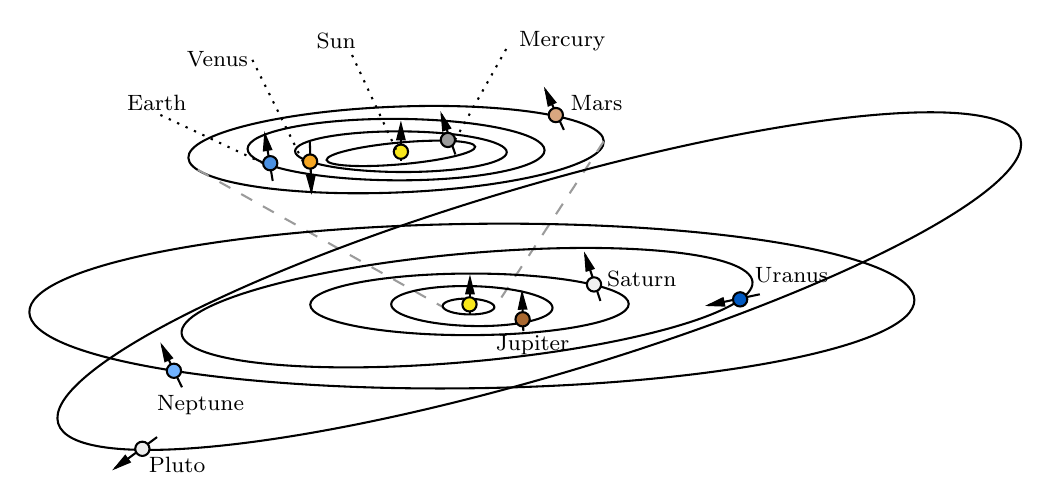
\begin{tikzpicture}[x=0.75pt,y=0.75pt,yscale=-1,xscale=1,scale=0.8]
			%uncomment if require: \path (0,896); %set diagram left start at 0, and has height of 896
			
			%Straight Lines [id:da8211588420815208] 
			\draw    (98.5,302) -- (73.11,320.81) ;
			\draw [shift={(71.5,322)}, rotate = 323.47] [fill={rgb, 255:red, 0; green, 0; blue, 0 }  ][line width=0.08]  [draw opacity=0] (12,-3) -- (0,0) -- (12,3) -- cycle    ;
			%Straight Lines [id:da9496415165487124] 
			\draw    (113.5,272) -- (101.37,246.8) ;
			\draw [shift={(100.5,245)}, rotate = 64.29] [fill={rgb, 255:red, 0; green, 0; blue, 0 }  ][line width=0.08]  [draw opacity=0] (12,-3) -- (0,0) -- (12,3) -- cycle    ;
			%Straight Lines [id:da04102336408187024] 
			\draw    (461.5,216) -- (430.46,222.58) ;
			\draw [shift={(428.5,223)}, rotate = 348.02] [fill={rgb, 255:red, 0; green, 0; blue, 0 }  ][line width=0.08]  [draw opacity=0] (12,-3) -- (0,0) -- (12,3) -- cycle    ;
			%Straight Lines [id:da8112468260893397] 
			\draw    (365.5,220) -- (356.28,192.15) ;
			\draw [shift={(355.65,190.26)}, rotate = 71.68] [fill={rgb, 255:red, 0; green, 0; blue, 0 }  ][line width=0.08]  [draw opacity=0] (12,-3) -- (0,0) -- (12,3) -- cycle    ;
			%Straight Lines [id:da7411431507138244] 
			\draw    (319.08,238.23) -- (318.3,215.28) ;
			\draw [shift={(318.23,213.28)}, rotate = 88.05] [fill={rgb, 255:red, 0; green, 0; blue, 0 }  ][line width=0.08]  [draw opacity=0] (12,-3) -- (0,0) -- (12,3) -- cycle    ;
			%Straight Lines [id:da04358678355558854] 
			\draw    (168.15,147.76) -- (163.48,119.73) ;
			\draw [shift={(163.15,117.76)}, rotate = 80.54] [fill={rgb, 255:red, 0; green, 0; blue, 0 }  ][line width=0.08]  [draw opacity=0] (12,-3) -- (0,0) -- (12,3) -- cycle    ;
			%Straight Lines [id:da2703507369125473] 
			\draw    (190.5,124) -- (191.44,154) ;
			\draw [shift={(191.5,156)}, rotate = 268.21] [fill={rgb, 255:red, 0; green, 0; blue, 0 }  ][line width=0.08]  [draw opacity=0] (12,-3) -- (0,0) -- (12,3) -- cycle    ;
			%Straight Lines [id:da8240782502736901] 
			\draw    (343.5,117) -- (332.34,92.82) ;
			\draw [shift={(331.5,91)}, rotate = 65.22] [fill={rgb, 255:red, 0; green, 0; blue, 0 }  ][line width=0.08]  [draw opacity=0] (12,-3) -- (0,0) -- (12,3) -- cycle    ;
			%Straight Lines [id:da6890915517546361] 
			\draw    (278.15,131.76) -- (269.81,107.65) ;
			\draw [shift={(269.15,105.76)}, rotate = 70.91] [fill={rgb, 255:red, 0; green, 0; blue, 0 }  ][line width=0.08]  [draw opacity=0] (12,-3) -- (0,0) -- (12,3) -- cycle    ;
			%Straight Lines [id:da7395453061348796] 
			\draw    (245.35,135.43) -- (245.35,113.36) ;
			\draw [shift={(245.35,111.36)}, rotate = 90] [fill={rgb, 255:red, 0; green, 0; blue, 0 }  ][line width=0.08]  [draw opacity=0] (12,-3) -- (0,0) -- (12,3) -- cycle    ;
			%Straight Lines [id:da5094077571228788] 
			\draw    (286.95,228.14) -- (286.95,206.08) ;
			\draw [shift={(286.95,204.08)}, rotate = 90] [fill={rgb, 255:red, 0; green, 0; blue, 0 }  ][line width=0.08]  [draw opacity=0] (12,-3) -- (0,0) -- (12,3) -- cycle    ;
			%Shape: Ellipse [id:dp24512703057052576] 
			\draw   (200.61,135.13) .. controls (200.29,131.52) and (220.06,126.81) .. (244.76,124.6) .. controls (269.47,122.39) and (289.76,123.52) .. (290.08,127.13) .. controls (290.41,130.73) and (270.64,135.44) .. (245.93,137.65) .. controls (221.22,139.86) and (200.93,138.73) .. (200.61,135.13) -- cycle ;
			%Shape: Ellipse [id:dp07875966526409162] 
			\draw   (181.6,129.81) .. controls (181.63,123.06) and (210.2,117.72) .. (245.41,117.89) .. controls (280.61,118.07) and (309.13,123.68) .. (309.1,130.44) .. controls (309.06,137.19) and (280.5,142.53) .. (245.29,142.36) .. controls (210.08,142.19) and (181.56,136.57) .. (181.6,129.81) -- cycle ;
			%Shape: Ellipse [id:dp24251866280106604] 
			\draw   (153,128.42) .. controls (153.05,118.21) and (193.14,110.12) .. (242.53,110.36) .. controls (291.93,110.6) and (331.93,119.08) .. (331.88,129.3) .. controls (331.83,139.51) and (291.75,147.6) .. (242.35,147.36) .. controls (192.96,147.12) and (152.95,138.64) .. (153,128.42) -- cycle ;
			%Shape: Ellipse [id:dp2431898785442428] 
			\draw   (117.34,133.86) .. controls (116.76,119.6) and (172.32,105.8) .. (241.41,103.04) .. controls (310.51,100.28) and (366.98,109.6) .. (367.55,123.86) .. controls (368.12,138.12) and (312.57,151.92) .. (243.48,154.68) .. controls (174.38,157.44) and (117.91,148.12) .. (117.34,133.86) -- cycle ;
			%Straight Lines [id:da43145661055313944] 
			\draw [color={rgb, 255:red, 155; green, 155; blue, 155 }  ,draw opacity=1 ] [dash pattern={on 4.5pt off 4.5pt}]  (123,141) -- (270.5,223.6) ;
			%Straight Lines [id:da4354517856700333] 
			\draw [color={rgb, 255:red, 155; green, 155; blue, 155 }  ,draw opacity=1 ] [dash pattern={on 4.5pt off 4.5pt}]  (367.55,123.86) -- (301.5,224.6) ;
			%Shape: Ellipse [id:dp22678424762696014] 
			\draw   (270.49,223) .. controls (270.55,220.36) and (277.58,218.39) .. (286.18,218.59) .. controls (294.78,218.8) and (301.7,221.1) .. (301.64,223.74) .. controls (301.57,226.38) and (294.55,228.35) .. (285.95,228.14) .. controls (277.35,227.94) and (270.43,225.64) .. (270.49,223) -- cycle ;
			%Shape: Ellipse [id:dp5401675301981814] 
			\draw   (239.51,221.94) .. controls (239.67,215.31) and (261.54,210.46) .. (288.37,211.1) .. controls (315.2,211.74) and (336.82,217.62) .. (336.67,224.25) .. controls (336.51,230.87) and (314.63,235.72) .. (287.8,235.09) .. controls (260.97,234.45) and (239.35,228.56) .. (239.51,221.94) -- cycle ;
			%Shape: Ellipse [id:dp32560698445253067] 
			\draw   (190.75,222.27) .. controls (190.72,212.03) and (233.64,203.63) .. (286.61,203.51) .. controls (339.58,203.39) and (382.53,211.6) .. (382.56,221.84) .. controls (382.58,232.08) and (339.66,240.48) .. (286.69,240.6) .. controls (233.73,240.72) and (190.77,232.51) .. (190.75,222.27) -- cycle ;
			%Shape: Ellipse [id:dp2985815219628527] 
			\draw   (113.29,239.61) .. controls (111.66,221.7) and (187.31,200.21) .. (282.25,191.62) .. controls (377.19,183.03) and (455.47,190.59) .. (457.09,208.5) .. controls (458.71,226.41) and (383.06,247.89) .. (288.12,256.48) .. controls (193.18,265.07) and (114.91,257.51) .. (113.29,239.61) -- cycle ;
			%Shape: Ellipse [id:dp591312419290327] 
			\draw   (38.94,293.72) .. controls (30,263.48) and (152.48,200.61) .. (312.5,153.31) .. controls (472.52,106) and (609.49,92.16) .. (618.43,122.4) .. controls (627.37,152.64) and (504.89,215.51) .. (344.87,262.82) .. controls (184.85,310.13) and (47.88,323.96) .. (38.94,293.72) -- cycle ;
			%Shape: Ellipse [id:dp10067762377581091] 
			\draw   (21.58,226.77) .. controls (21.2,199.43) and (140.22,175.63) .. (287.4,173.6) .. controls (434.59,171.57) and (554.22,192.08) .. (554.59,219.42) .. controls (554.97,246.75) and (435.96,270.55) .. (288.77,272.58) .. controls (141.58,274.61) and (21.96,254.1) .. (21.58,226.77) -- cycle ;
			%Shape: Circle [id:dp7051221927673568] 
			\draw  [fill={rgb, 255:red, 248; green, 231; blue, 28 }  ,fill opacity=1 ] (282.35,222.06) .. controls (282.35,219.68) and (284.28,217.76) .. (286.65,217.76) .. controls (289.03,217.76) and (290.95,219.68) .. (290.95,222.06) .. controls (290.95,224.43) and (289.03,226.36) .. (286.65,226.36) .. controls (284.28,226.36) and (282.35,224.43) .. (282.35,222.06) -- cycle ;
			%Shape: Circle [id:dp5598407154441705] 
			\draw  [fill={rgb, 255:red, 217; green, 167; blue, 128 }  ,fill opacity=1 ] (334.35,108.06) .. controls (334.35,105.68) and (336.28,103.76) .. (338.65,103.76) .. controls (341.03,103.76) and (342.95,105.68) .. (342.95,108.06) .. controls (342.95,110.43) and (341.03,112.36) .. (338.65,112.36) .. controls (336.28,112.36) and (334.35,110.43) .. (334.35,108.06) -- cycle ;
			%Shape: Circle [id:dp6930054681613842] 
			\draw  [fill={rgb, 255:red, 155; green, 155; blue, 155 }  ,fill opacity=1 ] (269.35,123.06) .. controls (269.35,120.68) and (271.28,118.76) .. (273.65,118.76) .. controls (276.03,118.76) and (277.95,120.68) .. (277.95,123.06) .. controls (277.95,125.43) and (276.03,127.36) .. (273.65,127.36) .. controls (271.28,127.36) and (269.35,125.43) .. (269.35,123.06) -- cycle ;
			%Shape: Circle [id:dp21627300573248331] 
			\draw  [fill={rgb, 255:red, 248; green, 231; blue, 28 }  ,fill opacity=1 ] (241.05,130.13) .. controls (241.05,127.75) and (242.97,125.83) .. (245.35,125.83) .. controls (247.72,125.83) and (249.65,127.75) .. (249.65,130.13) .. controls (249.65,132.5) and (247.72,134.43) .. (245.35,134.43) .. controls (242.97,134.43) and (241.05,132.5) .. (241.05,130.13) -- cycle ;
			%Shape: Circle [id:dp012927133977469918] 
			\draw  [fill={rgb, 255:red, 245; green, 166; blue, 35 }  ,fill opacity=1 ] (186.35,136.06) .. controls (186.35,133.68) and (188.28,131.76) .. (190.65,131.76) .. controls (193.03,131.76) and (194.95,133.68) .. (194.95,136.06) .. controls (194.95,138.43) and (193.03,140.36) .. (190.65,140.36) .. controls (188.28,140.36) and (186.35,138.43) .. (186.35,136.06) -- cycle ;
			%Shape: Circle [id:dp0871490317345176] 
			\draw  [fill={rgb, 255:red, 74; green, 144; blue, 226 }  ,fill opacity=1 ] (162.35,137.06) .. controls (162.35,134.68) and (164.28,132.76) .. (166.65,132.76) .. controls (169.03,132.76) and (170.95,134.68) .. (170.95,137.06) .. controls (170.95,139.43) and (169.03,141.36) .. (166.65,141.36) .. controls (164.28,141.36) and (162.35,139.43) .. (162.35,137.06) -- cycle ;
			%Shape: Circle [id:dp32814953802058966] 
			\draw  [fill={rgb, 255:red, 169; green, 104; blue, 48 }  ,fill opacity=1 ] (314.35,231.06) .. controls (314.35,228.68) and (316.28,226.76) .. (318.65,226.76) .. controls (321.03,226.76) and (322.95,228.68) .. (322.95,231.06) .. controls (322.95,233.43) and (321.03,235.36) .. (318.65,235.36) .. controls (316.28,235.36) and (314.35,233.43) .. (314.35,231.06) -- cycle ;
			%Shape: Circle [id:dp9839228391139974] 
			\draw  [fill={rgb, 255:red, 240; green, 240; blue, 240 }  ,fill opacity=1 ] (357.35,210.06) .. controls (357.35,207.68) and (359.28,205.76) .. (361.65,205.76) .. controls (364.03,205.76) and (365.95,207.68) .. (365.95,210.06) .. controls (365.95,212.43) and (364.03,214.36) .. (361.65,214.36) .. controls (359.28,214.36) and (357.35,212.43) .. (357.35,210.06) -- cycle ;
			%Shape: Circle [id:dp9672001498500622] 
			\draw  [fill={rgb, 255:red, 0; green, 89; blue, 194 }  ,fill opacity=1 ] (445.35,219.06) .. controls (445.35,216.68) and (447.28,214.76) .. (449.65,214.76) .. controls (452.03,214.76) and (453.95,216.68) .. (453.95,219.06) .. controls (453.95,221.43) and (452.03,223.36) .. (449.65,223.36) .. controls (447.28,223.36) and (445.35,221.43) .. (445.35,219.06) -- cycle ;
			%Shape: Circle [id:dp29146543527129] 
			\draw  [fill={rgb, 255:red, 112; green, 178; blue, 255 }  ,fill opacity=1 ] (104.35,262.06) .. controls (104.35,259.68) and (106.28,257.76) .. (108.65,257.76) .. controls (111.03,257.76) and (112.95,259.68) .. (112.95,262.06) .. controls (112.95,264.43) and (111.03,266.36) .. (108.65,266.36) .. controls (106.28,266.36) and (104.35,264.43) .. (104.35,262.06) -- cycle ;
			%Shape: Circle [id:dp5510820338538969] 
			\draw  [fill={rgb, 255:red, 237; green, 237; blue, 237 }  ,fill opacity=1 ] (85.35,309.06) .. controls (85.35,306.68) and (87.28,304.76) .. (89.65,304.76) .. controls (92.03,304.76) and (93.95,306.68) .. (93.95,309.06) .. controls (93.95,311.43) and (92.03,313.36) .. (89.65,313.36) .. controls (87.28,313.36) and (85.35,311.43) .. (85.35,309.06) -- cycle ;
			%Straight Lines [id:da7778523601327454] 
			\draw  [dash pattern={on 0.84pt off 2.51pt}]  (277.95,123.06) -- (309.5,67) ;
			%Straight Lines [id:da10233460351024082] 
			\draw  [dash pattern={on 0.84pt off 2.51pt}]  (242.44,128.86) -- (215.5,71) ;
			%Straight Lines [id:da5875895756534195] 
			\draw  [dash pattern={on 0.84pt off 2.51pt}]  (186.35,136.06) -- (162.07,87.22) -- (155.5,74) ;
			%Straight Lines [id:da522586322745608] 
			\draw  [dash pattern={on 0.84pt off 2.51pt}]  (100.5,108) -- (162.35,137.06) ;
			
			% Text Node
			\draw (91.65,312.06) node [anchor=north west][inner sep=0.75pt]  [font=\footnotesize] [align=left] {Pluto};
			% Text Node
			\draw (96.65,275.06) node [anchor=north west][inner sep=0.75pt]  [font=\footnotesize] [align=left] {Neptune};
			% Text Node
			\draw (300.65,239.06) node [anchor=north west][inner sep=0.75pt]  [font=\footnotesize] [align=left] {Jupiter};
			% Text Node
			\draw (367.65,200.06) node [anchor=north west][inner sep=0.75pt]  [font=\footnotesize] [align=left] {Saturn};
			% Text Node
			\draw (456.65,198.06) node [anchor=north west][inner sep=0.75pt]  [font=\footnotesize] [align=left] {Uranus};
			% Text Node
			\draw (345.65,94.06) node [anchor=north west][inner sep=0.75pt]  [font=\footnotesize] [align=left] {Mars};
			% Text Node
			\draw (314.65,56.06) node [anchor=north west][inner sep=0.75pt]  [font=\footnotesize] [align=left] {Mercury};
			% Text Node
			\draw (192.65,57.06) node [anchor=north west][inner sep=0.75pt]  [font=\footnotesize] [align=left] {Sun};
			% Text Node
			\draw (114.65,68.06) node [anchor=north west][inner sep=0.75pt]  [font=\footnotesize] [align=left] {Venus};
			% Text Node
			\draw (78.65,94.06) node [anchor=north west][inner sep=0.75pt]  [font=\footnotesize] [align=left] {Earth};
			
			\end{tikzpicture}
			\vspace*{3mm}
			\caption{Planets spin and angle relatively to the ecliptic plane}
		\end{figure}
		
		\item The orbits precess around the Sun as shown in the following figure (see further below for the mathematical proof in the case of a 2-body system):
		\begin{figure}[H]
			\centering
			\includegraphics{img/cosmology/orbit_precession.jpg}	
			\caption{Orbit precession example}
		\end{figure}
		
		\item The planets have an helicity trajectory "behind" the movement of the Sun around the center of our Galaxy and the ecliptic has an angle of approximately $60^\circ$ ($\pi/3$ [rad]) relatively to the perpendicular of the Sun movement as visible in the figure below:
		\begin{figure}[H]
			\centering
			\includegraphics{img/cosmology/solar_system_vortex.jpg}	
			\caption{Planets with orbits following the Sun in its movement}
		\end{figure}
		and the planets are therefore sometimes in front of the Sun and sometimes behind.
		
		Because of the movement of our Sun around the center of our Galaxy and some far-distant interactions in-between other celestial objects, the reader must understand that constellations doesn't appear always as there are today! The geometry change and even on the very long term... some stars of the constellations may disappear (as they have a finished lifetime!):
		\begin{figure}[H]
			\centering
			\includegraphics[width=0.8\textwidth]{img/cosmology/constellation_movements.jpg}	
			\caption[Constellations throughout ages]{Constellations throughout ages with years based on Gregorian calendar (author: Martin Vargic)}
		\end{figure}
		For scales remember that hominids exist since only $7$ millions years (at the date we write these lines...) and Homo Sapiens since only $300,000$ years ago.
		
		Not only apparent relative distances between stars within a constellation (and every other star!) changes over time but also the absolute distance between them and Earth is in reality an illusion that also changes over time !! For example at naked eye Orion's constellation stars may seem all lying in an identical plane (and at a human scale life not moving...):
		\begin{figure}[H]
			\begin{minipage}{0.3\linewidth}
				\centering  % redundant
				\includegraphics[height=6.5cm]{img/cosmology/orion_constellation_stellarium.png}
				\caption[Orion stellarium representation]{Orion stellarium representation (authors: Roger Sinnott \& Rick Fienberg)}
			\end{minipage}%
				\hfill% not: "\hspace{0.5cm}"
				\begin{minipage}{0.3\linewidth}
				\centering  % redundant
				\includegraphics[height=6.5cm]{img/cosmology/orion_constellation_ground_photography_short_pose.jpg}
				\vspace*{1mm}
				\caption[Orion short pose photography]{Orion short pose photography \\(author: Till Credner)}
			\end{minipage}%
				\hfill% not: "\hspace{0.5cm}"
				\begin{minipage}{0.3\linewidth}
				\centering  % redundant
				\includegraphics[height=6.5cm]{img/cosmology/orion_constellation_ground_photography_long_pose.jpg}
				\vspace*{1mm}
				\caption[Orion long pose photography]{Orion long pose photography\\(author: Rogelio Bernal Andreo)}
			\end{minipage}
		\end{figure}
		But in reality the various stars are at quite different distances as depicted in the figure below (the various stars of Orion's constellation are moving in various directions at speeds between $10$ and $30\;[\text{km}\cdot\text{s}^{-1}]$, hence between $20$ and $75$ billion kilometres in an average human lifetime, but that's tiny compared to a light-year distance and this is why visible changes at naked eyes takes tens of thousands of years...much more than the actual record of a single human lifetime!):
		\begin{figure}[H]
		\centering
		% Gradient Info

		\tikzset {_qxh0ego12/.code = {\pgfsetadditionalshadetransform{ \pgftransformshift{\pgfpoint{0 bp } { 0 bp }  }  \pgftransformscale{1 }  }}}
		\pgfdeclareradialshading{_h7f60dzk2}{\pgfpoint{0bp}{0bp}}{rgb(0bp)=(0.92,0.95,0.97);
		rgb(0.08117079734802246bp)=(0.92,0.95,0.97);
		rgb(25bp)=(0.77,0.88,0.95);
		rgb(400bp)=(0.77,0.88,0.95)}
		
		% Gradient Info
		  
		\tikzset {_38yrjblb4/.code = {\pgfsetadditionalshadetransform{ \pgftransformshift{\pgfpoint{0 bp } { 0 bp }  }  \pgftransformscale{1 }  }}}
		\pgfdeclareradialshading{_q78aiiwjf}{\pgfpoint{0bp}{0bp}}{rgb(0bp)=(0.56,0.07,1);
		rgb(0.17045651163373673bp)=(0.56,0.07,1);
		rgb(19.00060875075204bp)=(1,1,1);
		rgb(400bp)=(1,1,1)}
		\resizebox{\textwidth}{!}{
		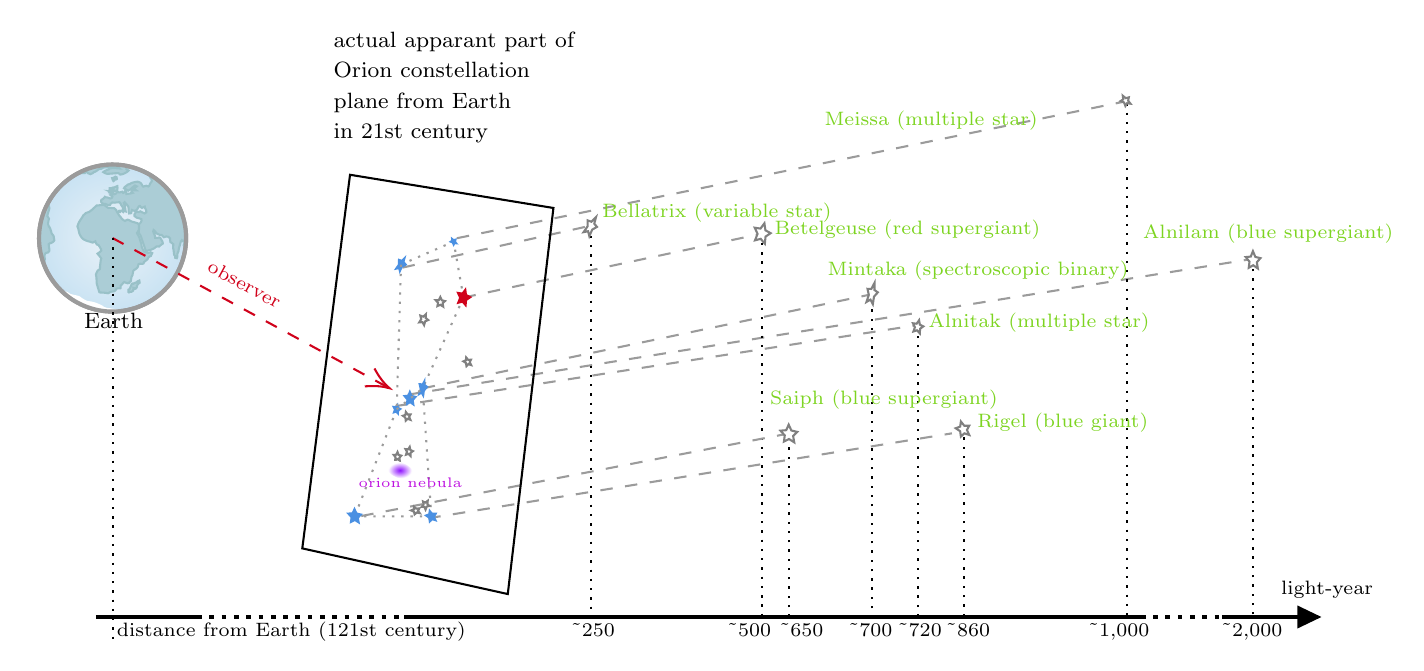
\begin{tikzpicture}[x=0.75pt,y=0.75pt,yscale=-1,xscale=1]
		%uncomment if require: \path (0,884); %set diagram left start at 0, and has height of 884
		
		%Straight Lines [id:da8954989404295903] 
		\draw [color={rgb, 255:red, 155; green, 155; blue, 155 }  ,draw opacity=1 ] [dash pattern={on 4.5pt off 4.5pt}]  (193.14,316.33) -- (598.37,251.19) ;
		%Straight Lines [id:da1497092614069595] 
		\draw  [dash pattern={on 0.84pt off 2.51pt}]  (281.33,235.31) -- (281.33,422.73) ;
		%Straight Lines [id:da7720257031182898] 
		\draw [color={rgb, 255:red, 0; green, 0; blue, 0 }  ,draw opacity=1 ] [dash pattern={on 0.84pt off 2.51pt}]  (539.74,175.92) -- (539.74,423.1) ;
		%Straight Lines [id:da7028549050434356] 
		\draw [color={rgb, 255:red, 0; green, 0; blue, 0 }  ,draw opacity=1 ] [dash pattern={on 0.84pt off 2.51pt}]  (363.82,238.73) -- (363.82,423.43) ;
		%Straight Lines [id:da11685200382588157] 
		\draw  [dash pattern={on 0.84pt off 2.51pt}]  (376.82,423.23) -- (376.82,335.37) ;
		%Straight Lines [id:da6730799246215375] 
		\draw [color={rgb, 255:red, 0; green, 0; blue, 0 }  ,draw opacity=1 ] [dash pattern={on 0.84pt off 2.51pt}]  (461.35,422.88) -- (461.35,334.95) ;
		%Straight Lines [id:da05562325842555982] 
		\draw [color={rgb, 255:red, 0; green, 0; blue, 0 }  ,draw opacity=1 ] [dash pattern={on 0.84pt off 2.51pt}]  (416.77,423.73) -- (416.77,267.83) ;
		%Straight Lines [id:da4080771467329807] 
		\draw [color={rgb, 255:red, 0; green, 0; blue, 0 }  ,draw opacity=1 ] [dash pattern={on 0.84pt off 2.51pt}]  (438.88,423.1) -- (438.88,283.68) ;
		%Straight Lines [id:da7915051483941069] 
		\draw [color={rgb, 255:red, 0; green, 0; blue, 0 }  ,draw opacity=1 ] [dash pattern={on 0.84pt off 2.51pt}]  (600.53,422.19) -- (600.53,253.95) ;
		%Straight Lines [id:da9469183523580174] 
		\draw [color={rgb, 255:red, 155; green, 155; blue, 155 }  ,draw opacity=1 ] [dash pattern={on 4.5pt off 4.5pt}]  (190.67,255.09) -- (279.82,235.23) ;
		%Straight Lines [id:da3499518994850317] 
		\draw [color={rgb, 255:red, 155; green, 155; blue, 155 }  ,draw opacity=1 ] [dash pattern={on 4.5pt off 4.5pt}]  (216.84,240.94) -- (543.41,174.1) ;
		%Straight Lines [id:da8735857783511269] 
		\draw [color={rgb, 255:red, 155; green, 155; blue, 155 }  ,draw opacity=1 ] [dash pattern={on 4.5pt off 4.5pt}]  (220.03,269.53) -- (363.82,238.73) ;
		%Straight Lines [id:da6205737060478944] 
		\draw [color={rgb, 255:red, 155; green, 155; blue, 155 }  ,draw opacity=1 ] [dash pattern={on 4.5pt off 4.5pt}]  (187.33,321.83) -- (439.91,282.6) ;
		%Straight Lines [id:da1442699388067834] 
		\draw [color={rgb, 255:red, 155; green, 155; blue, 155 }  ,draw opacity=1 ] [dash pattern={on 4.5pt off 4.5pt}]  (200.37,313.28) -- (415.32,268.23) ;
		%Straight Lines [id:da19536351324407653] 
		\draw [color={rgb, 255:red, 155; green, 155; blue, 155 }  ,draw opacity=1 ] [dash pattern={on 4.5pt off 4.5pt}]  (170.77,374.78) -- (380.82,334.23) ;
		%Straight Lines [id:da829729197083553] 
		\draw [color={rgb, 255:red, 155; green, 155; blue, 155 }  ,draw opacity=1 ] [dash pattern={on 4.5pt off 4.5pt}]  (203.09,375.85) -- (455.35,334.95) ;
		%Straight Lines [id:da8500797301952514] 
		\draw [color={rgb, 255:red, 155; green, 155; blue, 155 }  ,draw opacity=1 ] [dash pattern={on 0.84pt off 2.51pt}]  (187.84,323.39) -- (167.62,374.92) ;
		%Straight Lines [id:da5942808850437651] 
		\draw [color={rgb, 255:red, 155; green, 155; blue, 155 }  ,draw opacity=1 ] [dash pattern={on 0.84pt off 2.51pt}]  (204.55,374.95) -- (167.62,374.92) ;
		%Straight Lines [id:da40220557101554544] 
		\draw [color={rgb, 255:red, 155; green, 155; blue, 155 }  ,draw opacity=1 ] [dash pattern={on 0.84pt off 2.51pt}]  (204.55,374.95) -- (200.37,313.28) ;
		%Straight Lines [id:da7631780523951637] 
		\draw [color={rgb, 255:red, 155; green, 155; blue, 155 }  ,draw opacity=1 ] [dash pattern={on 0.84pt off 2.51pt}]  (220.03,269.53) -- (200.37,313.28) ;
		%Straight Lines [id:da7724916802042507] 
		\draw [color={rgb, 255:red, 155; green, 155; blue, 155 }  ,draw opacity=1 ] [dash pattern={on 0.84pt off 2.51pt}]  (220.03,269.53) -- (215.29,242.58) ;
		%Straight Lines [id:da48971379748984467] 
		\draw [color={rgb, 255:red, 155; green, 155; blue, 155 }  ,draw opacity=1 ] [dash pattern={on 0.84pt off 2.51pt}]  (189.94,253.62) -- (215.29,242.58) ;
		%Shape: Circle [id:dp44519081268975236] 
		\path  [shading=_h7f60dzk2,_qxh0ego12] (17.58,229.05) .. controls (24.11,210.61) and (44.34,200.96) .. (62.78,207.48) .. controls (81.21,214.01) and (90.87,234.24) .. (84.34,252.68) .. controls (77.82,271.11) and (57.58,280.77) .. (39.15,274.24) .. controls (20.71,267.72) and (11.06,247.48) .. (17.58,229.05) -- cycle ; % for fading 
		 \draw  [color={rgb, 255:red, 155; green, 155; blue, 155 }  ,draw opacity=1 ][line width=1.5]  (17.58,229.05) .. controls (24.11,210.61) and (44.34,200.96) .. (62.78,207.48) .. controls (81.21,214.01) and (90.87,234.24) .. (84.34,252.68) .. controls (77.82,271.11) and (57.58,280.77) .. (39.15,274.24) .. controls (20.71,267.72) and (11.06,247.48) .. (17.58,229.05) -- cycle ; % for border 
		
		%Shape: Polygon Curved [id:ds6524753250348416] 
		\draw  [color={rgb, 255:red, 153; green, 193; blue, 200 }  ,draw opacity=1 ][fill={rgb, 255:red, 171; green, 205; blue, 214 }  ,fill opacity=1 ] (60.19,263.06) .. controls (60.59,262.36) and (60.69,263.04) .. (61.05,262.87) .. controls (61.41,262.7) and (61.17,262.62) .. (61.49,262.48) .. controls (61.82,262.33) and (61.96,262.43) .. (62.3,262.31) .. controls (62.64,262.2) and (62.66,261.87) .. (62.89,261.77) .. controls (63.12,261.68) and (63.48,261.09) .. (63.85,261.32) .. controls (64.22,261.54) and (64.14,262.08) .. (64.02,262.37) .. controls (63.9,262.67) and (63.49,262.7) .. (63.19,263.03) .. controls (62.9,263.35) and (62.68,263.92) .. (62.64,264.03) .. controls (62.59,264.14) and (63,264.55) .. (62.31,265.1) .. controls (61.62,265.66) and (61.84,265.16) .. (61.61,264.96) .. controls (61.39,264.75) and (61.13,264.7) .. (60.96,264.83) .. controls (60.8,264.95) and (61.25,265.57) .. (60.8,266.26) .. controls (60.36,266.95) and (60,266.62) .. (59.43,266.77) .. controls (58.86,266.92) and (58.73,267.33) .. (58.56,266.82) .. controls (58.4,266.31) and (58.32,266.11) .. (58.6,265.73) .. controls (58.89,265.36) and (59.11,265.53) .. (59.23,265.36) .. controls (59.36,265.19) and (59.79,263.77) .. (60.19,263.06) -- cycle ;
		%Shape: Polygon Curved [id:ds0792022658104925] 
		\draw  [color={rgb, 255:red, 153; green, 193; blue, 200 }  ,draw opacity=1 ][fill={rgb, 255:red, 171; green, 205; blue, 214 }  ,fill opacity=1 ] (52.28,211.28) .. controls (52.67,211.19) and (53.32,211.73) .. (53.02,212.42) .. controls (52.73,213.11) and (52.94,212.18) .. (52.33,212.54) .. controls (51.73,212.9) and (51.47,213.71) .. (51.38,213.4) .. controls (51.29,213.09) and (50.64,212.45) .. (50.75,211.96) .. controls (50.86,211.47) and (51.14,211.96) .. (51.33,211.87) .. controls (51.51,211.78) and (51.89,211.37) .. (52.28,211.28) -- cycle ;
		%Shape: Polygon Curved [id:ds7018460039443064] 
		\draw  [color={rgb, 255:red, 153; green, 193; blue, 200 }  ,draw opacity=1 ][fill={rgb, 255:red, 171; green, 205; blue, 214 }  ,fill opacity=1 ] (54.58,227.71) .. controls (54.97,227.62) and (54.75,228.07) .. (54.59,228.36) .. controls (54.44,228.66) and (54.27,228.45) .. (54,228.35) .. controls (53.74,228.26) and (53.75,228.07) .. (53.92,227.73) .. controls (54.09,227.39) and (54.19,227.8) .. (54.58,227.71) -- cycle ;
		%Shape: Polygon Curved [id:ds5002658553340216] 
		\draw  [color={rgb, 255:red, 153; green, 193; blue, 200 }  ,draw opacity=1 ][fill={rgb, 255:red, 171; green, 205; blue, 214 }  ,fill opacity=1 ] (46.92,205.74) .. controls (48.51,205.61) and (54.44,205.66) .. (55.58,205.81) .. controls (56.72,205.97) and (57.09,205.97) .. (57.97,206.17) .. controls (58.85,206.36) and (60.19,206.79) .. (59.68,206.67) .. controls (59.18,206.55) and (57.95,206.63) .. (57.65,206.8) .. controls (57.34,206.97) and (57.49,207.57) .. (57.59,207.67) .. controls (57.69,207.78) and (58.65,208.3) .. (58.69,208.36) .. controls (58.73,208.42) and (58.01,208.95) .. (57.78,209.09) .. controls (57.56,209.23) and (56.55,209.82) .. (56.25,209.89) .. controls (55.96,209.96) and (54.85,210.37) .. (54.67,210.28) .. controls (54.5,210.18) and (53.92,209.63) .. (53.78,209.56) .. controls (53.65,209.49) and (52.8,209.7) .. (52.56,209.63) .. controls (52.33,209.56) and (51.12,209.74) .. (50.92,209.75) .. controls (50.71,209.76) and (48.49,209.97) .. (48.27,209.91) .. controls (48.05,209.85) and (46.52,209.33) .. (46.51,209.08) .. controls (46.51,208.83) and (46.56,208.78) .. (47.13,208.6) .. controls (47.7,208.41) and (48.54,207.86) .. (49.12,207.76) .. controls (49.7,207.65) and (49.58,207.27) .. (49.8,207.25) .. controls (50.02,207.23) and (50.79,207.19) .. (51.29,207.15) .. controls (51.8,207.11) and (52.25,207.16) .. (52.86,207.21) .. controls (53.48,207.25) and (54.29,207.35) .. (54.4,207.34) .. controls (54.51,207.32) and (53.77,206.81) .. (53.61,206.76) .. controls (53.45,206.7) and (52.63,206.41) .. (51.85,206.38) .. controls (51.06,206.35) and (50.08,206.18) .. (49.98,206.17) .. controls (49.88,206.16) and (48.77,206.67) .. (48.61,206.68) .. controls (48.44,206.69) and (46.47,206.89) .. (46.44,206.91) .. controls (46.4,206.93) and (45.84,207.3) .. (45.59,207.46) .. controls (45.34,207.61) and (44.63,207.57) .. (44.37,207.67) .. controls (44.12,207.77) and (43.12,208.67) .. (42.84,208.77) .. controls (42.55,208.87) and (42.24,208.94) .. (41.91,209.14) .. controls (41.59,209.33) and (41.37,209.61) .. (41.34,209.63) .. controls (41.31,209.65) and (40.21,210.03) .. (40.19,210.07) .. controls (40.17,210.12) and (39.64,209.59) .. (39.23,209.68) .. controls (38.82,209.77) and (38.98,209.48) .. (38.47,209.02) .. controls (37.96,208.56) and (38.24,209.43) .. (37.63,209.57) .. controls (37.02,209.7) and (36.42,209.63) .. (35.83,209.58) .. controls (35.25,209.53) and (35.05,209.45) .. (35.08,209.31) .. controls (35.12,209.16) and (39.61,207.27) .. (40.05,207.23) .. controls (40.49,207.19) and (45.33,205.87) .. (46.92,205.74) -- cycle ;
		%Shape: Polygon Curved [id:ds6145841697729744] 
		\draw  [color={rgb, 255:red, 153; green, 193; blue, 200 }  ,draw opacity=1 ][fill={rgb, 255:red, 171; green, 205; blue, 214 }  ,fill opacity=1 ] (51.38,217.61) .. controls (51.47,217.29) and (51.23,217.46) .. (51.48,217.05) .. controls (51.72,216.64) and (51.35,216.6) .. (51.5,216.56) .. controls (51.65,216.52) and (52.17,216.65) .. (52.33,216.21) .. controls (52.48,215.77) and (53.12,215.78) .. (53.25,215.84) .. controls (53.38,215.9) and (53.24,216.39) .. (53.34,216.71) .. controls (53.44,217.04) and (53.42,217.51) .. (53.22,217.77) .. controls (53.02,218.03) and (52.56,217.93) .. (52.35,218.11) .. controls (52.14,218.28) and (51.68,218.1) .. (51.44,218.58) .. controls (51.2,219.05) and (51.04,219.09) .. (50.98,219.16) .. controls (50.92,219.24) and (51.31,219.23) .. (51.11,219.51) .. controls (51.04,219.6) and (50.96,219.63) .. (50.86,219.63) .. controls (50.63,219.61) and (50.32,219.42) .. (49.94,219.15) .. controls (49.39,218.75) and (49.33,219.17) .. (49.7,218.71) .. controls (50.07,218.25) and (49.11,218.45) .. (49.39,218.3) .. controls (49.68,218.16) and (50.59,218.61) .. (50.83,218.32) .. controls (51.07,218.02) and (51.3,217.94) .. (51.38,217.61) -- cycle ;
		%Shape: Polygon Curved [id:ds44812350719480265] 
		\draw  [color={rgb, 255:red, 153; green, 193; blue, 200 }  ,draw opacity=1 ][fill={rgb, 255:red, 171; green, 205; blue, 214 }  ,fill opacity=1 ] (50.33,216.79) .. controls (50.71,216.7) and (51.12,216.38) .. (50.83,217.07) .. controls (50.53,217.76) and (51.14,217.12) .. (50.54,217.48) .. controls (49.93,217.84) and (49.77,218.22) .. (49.68,217.91) .. controls (49.59,217.6) and (49.39,217.79) .. (49.5,217.3) .. controls (49.61,216.81) and (49.34,216.9) .. (49.53,216.81) .. controls (49.72,216.72) and (49.94,216.88) .. (50.33,216.79) -- cycle ;
		%Shape: Polygon Curved [id:ds5273123276726659] 
		\draw  [color={rgb, 255:red, 153; green, 193; blue, 200 }  ,draw opacity=1 ][fill={rgb, 255:red, 171; green, 205; blue, 214 }  ,fill opacity=1 ] (17.45,230) .. controls (17.64,229.29) and (19.23,224.96) .. (19.71,224.88) .. controls (20.18,224.8) and (20.12,225.03) .. (20.26,225.42) .. controls (20.4,225.81) and (20.51,226.34) .. (20.52,226.51) .. controls (20.53,226.68) and (19.49,229.98) .. (19.53,230.29) .. controls (19.57,230.6) and (20.35,231.08) .. (20.31,231.46) .. controls (20.27,231.85) and (19.75,233.75) .. (19.95,234.32) .. controls (20.14,234.89) and (20.28,235.29) .. (20.28,235.34) .. controls (20.29,235.39) and (20.11,235.06) .. (20.49,235.46) .. controls (20.87,235.86) and (21.06,235.96) .. (21.02,236.49) .. controls (20.98,237.03) and (21.34,237.48) .. (21.34,237.55) .. controls (21.34,237.62) and (21.19,238.26) .. (21.58,238.58) .. controls (21.96,238.9) and (22.36,239.74) .. (22.5,239.76) .. controls (22.65,239.77) and (22.58,240.47) .. (22.71,240.87) .. controls (22.83,241.28) and (22.96,241.71) .. (22.91,241.99) .. controls (22.86,242.27) and (22.34,242.62) .. (22.24,242.75) .. controls (22.14,242.88) and (21.64,243.27) .. (21.27,243.25) .. controls (20.89,243.23) and (20.24,243.69) .. (20.19,243.77) .. controls (20.14,243.84) and (20.35,245.36) .. (20.39,245.58) .. controls (20.43,245.8) and (20.64,246.92) .. (20.53,247.02) .. controls (20.42,247.11) and (19.95,247.8) .. (19.85,247.82) .. controls (19.75,247.85) and (19.12,247.96) .. (18.78,248.04) .. controls (18.43,248.12) and (18.25,248.95) .. (18.11,249.5) .. controls (17.97,250.04) and (18.37,250.59) .. (18.35,250.93) .. controls (18.33,251.27) and (17.91,253.13) .. (17.88,253.1) .. controls (17.85,253.07) and (16.02,245.97) .. (15.87,244.72) .. controls (15.71,243.47) and (15.55,240.1) .. (15.98,237.09) .. controls (16.41,234.09) and (17.25,230.7) .. (17.45,230) -- cycle ;
		%Shape: Polygon Curved [id:ds8147570066327621] 
		\draw  [color={rgb, 255:red, 153; green, 193; blue, 200 }  ,draw opacity=1 ][fill={rgb, 255:red, 171; green, 205; blue, 214 }  ,fill opacity=1 ] (63.65,234.33) .. controls (63.66,234.06) and (64.35,233.69) .. (64.54,233.35) .. controls (64.74,233.02) and (65.19,232.01) .. (64.87,231.73) .. controls (64.54,231.44) and (64.02,231.36) .. (63.64,231.32) .. controls (63.26,231.28) and (62.93,231.37) .. (62.55,231.03) .. controls (62.17,230.7) and (61.61,230.6) .. (61.49,230.21) .. controls (61.38,229.82) and (61.17,229.65) .. (61.54,229.38) .. controls (61.91,229.12) and (61.87,228.56) .. (62.2,228.33) .. controls (62.53,228.1) and (63.48,228.3) .. (63.55,228.31) .. controls (63.62,228.31) and (63.95,227.9) .. (64.32,227.98) .. controls (64.69,228.06) and (64.61,228.07) .. (65.09,228.39) .. controls (65.58,228.72) and (65.93,228.99) .. (66.42,229.01) .. controls (66.91,229.04) and (66.97,228.86) .. (67.21,228.45) .. controls (67.46,228.04) and (67.32,227.71) .. (67.16,227.39) .. controls (67,227.08) and (66.89,227.24) .. (66.66,226.51) .. controls (66.42,225.78) and (66.82,225.77) .. (66.45,225.69) .. controls (66.08,225.61) and (65.49,226.36) .. (65.11,226.36) .. controls (64.74,226.36) and (64.19,225.42) .. (64.17,225.38) .. controls (64.14,225.34) and (63.59,225.32) .. (63.36,225.99) .. controls (63.12,226.65) and (62.7,227.24) .. (62.45,227.41) .. controls (62.21,227.58) and (61.75,227.68) .. (61.54,227.74) .. controls (61.34,227.79) and (60.47,227.36) .. (60.29,227.34) .. controls (60.1,227.32) and (60.16,228.54) .. (59.93,228.86) .. controls (59.69,229.17) and (59.22,229.2) .. (58.93,229) .. controls (58.64,228.81) and (58.6,228.17) .. (58.68,228.02) .. controls (58.76,227.86) and (58.65,227.3) .. (58.68,227.06) .. controls (58.71,226.83) and (58.72,226.53) .. (58.65,226.3) .. controls (58.58,226.08) and (58.53,225.74) .. (58.53,225.66) .. controls (58.52,225.58) and (58.21,225.44) .. (58.07,225) .. controls (57.92,224.57) and (57.74,224.52) .. (57.43,224.28) .. controls (57.11,224.04) and (57.07,223.59) .. (56.79,223.55) .. controls (56.5,223.52) and (56.33,223.51) .. (56.35,223.95) .. controls (56.37,224.38) and (56.66,224.75) .. (56.71,225.02) .. controls (56.77,225.29) and (57.29,225.87) .. (57.01,226.22) .. controls (56.74,226.57) and (57.6,227.98) .. (57.29,228.02) .. controls (56.97,228.06) and (56.72,227.58) .. (56.49,227.74) .. controls (56.26,227.9) and (56.25,228.31) .. (56.09,228.3) .. controls (55.94,228.29) and (55.36,227.93) .. (55.38,227.68) .. controls (55.39,227.42) and (55.73,227.4) .. (55.94,227.29) .. controls (56.15,227.17) and (56.16,226.82) .. (55.97,226.5) .. controls (55.78,226.19) and (55.85,226.27) .. (55.73,225.77) .. controls (55.61,225.27) and (55.36,225.41) .. (55.22,225.09) .. controls (55.09,224.77) and (54.9,224.49) .. (54.74,224.12) .. controls (54.57,223.74) and (54.79,223.87) .. (54.31,223.62) .. controls (53.84,223.37) and (53.42,223.55) .. (53.07,223.63) .. controls (52.71,223.71) and (52.22,223.92) .. (51.95,223.83) .. controls (51.68,223.74) and (50.55,223.7) .. (50.81,223.68) .. controls (51.07,223.65) and (50.36,224.08) .. (50.12,224.23) .. controls (49.87,224.37) and (50.03,224.69) .. (49.79,224.86) .. controls (49.55,225.02) and (48.96,225.01) .. (48.8,225) .. controls (48.64,225) and (47.63,224.33) .. (47.59,224.45) .. controls (47.56,224.57) and (46.41,224.28) .. (46.18,224.23) .. controls (45.95,224.18) and (45.48,223.52) .. (45.49,223.51) .. controls (45.5,223.49) and (45.38,222.55) .. (45.58,222.42) .. controls (45.77,222.29) and (46.44,221.95) .. (46.51,221.9) .. controls (46.57,221.86) and (47.19,220.97) .. (47.28,220.98) .. controls (47.38,220.99) and (47.63,221.24) .. (47.74,221.25) .. controls (47.84,221.25) and (48.41,221.31) .. (48.51,221.32) .. controls (48.6,221.33) and (49.03,221.42) .. (49.1,221.48) .. controls (49.16,221.54) and (49.74,221.79) .. (49.83,221.79) .. controls (49.93,221.79) and (50.56,221.57) .. (50.58,221.51) .. controls (50.6,221.46) and (50.86,221) .. (50.89,220.92) .. controls (50.91,220.85) and (49.96,220.14) .. (49.94,220.09) .. controls (49.92,220.04) and (50.44,219.76) .. (50.54,219.8) .. controls (50.64,219.84) and (51.16,219.82) .. (51.22,219.85) .. controls (51.28,219.88) and (51.98,219.77) .. (52.01,219.73) .. controls (52.03,219.68) and (52.6,219.46) .. (52.62,219.4) .. controls (52.65,219.33) and (53.01,218.8) .. (53.05,218.75) .. controls (53.09,218.7) and (53.8,218.68) .. (53.84,218.78) .. controls (53.87,218.88) and (54.54,218.93) .. (54.61,218.85) .. controls (54.68,218.78) and (55.54,218.52) .. (55.62,218.52) .. controls (55.71,218.52) and (56,219.05) .. (56.06,219.12) .. controls (56.11,219.2) and (56.68,219.11) .. (56.69,218.82) .. controls (56.7,218.53) and (56.82,218.02) .. (57.15,217.94) .. controls (57.48,217.85) and (57.63,218.55) .. (57.53,218.82) .. controls (57.44,219.08) and (57.56,219.58) .. (57.62,219.63) .. controls (57.68,219.67) and (58.23,219.54) .. (58.39,219.55) .. controls (58.55,219.56) and (59.41,219.31) .. (59.78,219.36) .. controls (60.15,219.42) and (60.57,219.36) .. (60.62,219.1) .. controls (60.67,218.83) and (60.21,218.93) .. (60.03,218.66) .. controls (59.85,218.38) and (60.05,218.17) .. (60.39,217.79) .. controls (60.72,217.41) and (62.26,218.32) .. (62.35,217.87) .. controls (62.43,217.41) and (61.31,217.53) .. (61.08,217.24) .. controls (60.85,216.95) and (62.7,216.07) .. (62.65,215.94) .. controls (62.61,215.81) and (62.16,215.52) .. (61.75,215.52) .. controls (61.35,215.53) and (60.99,216.29) .. (60.64,216.38) .. controls (60.29,216.47) and (60.19,216.67) .. (59.85,217.2) .. controls (59.51,217.73) and (58.88,217.9) .. (58.51,218.02) .. controls (58.15,218.14) and (57.73,217.29) .. (57.4,217.38) .. controls (57.06,217.47) and (56.6,217.41) .. (56.47,216.9) .. controls (56.34,216.39) and (57.34,215.91) .. (57.34,215.9) .. controls (57.34,215.89) and (57.97,215.4) .. (58.03,215.35) .. controls (58.09,215.3) and (58.74,214.71) .. (59.2,214.83) .. controls (59.65,214.94) and (59.77,214.45) .. (60.14,214.31) .. controls (60.52,214.17) and (61.35,214.07) .. (61.8,213.85) .. controls (62.25,213.63) and (62.7,213.73) .. (63.05,213.69) .. controls (63.4,213.65) and (64.21,214.14) .. (64.27,214.18) .. controls (64.34,214.21) and (65.04,214.69) .. (65.12,215.17) .. controls (65.19,215.65) and (65.67,216.06) .. (65.74,216.09) .. controls (65.8,216.11) and (67.08,215.62) .. (67.14,215.64) .. controls (67.2,215.66) and (67.94,216.01) .. (68.26,215.99) .. controls (68.59,215.96) and (68.63,215.6) .. (68.66,215.58) .. controls (68.68,215.55) and (69.13,214.5) .. (69.15,214.46) .. controls (69.17,214.42) and (69.79,213.64) .. (69.93,213.39) .. controls (70.07,213.14) and (69.94,212.46) .. (69.62,212.28) .. controls (69.31,212.11) and (69.13,211.74) .. (69.13,211.71) .. controls (69.13,211.68) and (69.55,210.83) .. (69.55,210.82) .. controls (69.56,210.8) and (78.02,215.46) .. (82.92,225.66) .. controls (87.82,235.86) and (86.21,244.76) .. (86.21,244.78) .. controls (86.2,244.8) and (85.13,244.6) .. (85.25,244.24) .. controls (85.38,243.89) and (85.49,243.43) .. (85.57,243.21) .. controls (85.65,242.99) and (85.45,242.04) .. (85.4,242) .. controls (85.35,241.96) and (84.91,242.36) .. (84.78,242.33) .. controls (84.65,242.31) and (84.37,241.86) .. (84.35,241.88) .. controls (84.32,241.9) and (83.89,242.5) .. (83.86,242.55) .. controls (83.83,242.6) and (83.59,243.39) .. (83.57,243.5) .. controls (83.56,243.61) and (83.35,244.43) .. (83.29,244.59) .. controls (83.23,244.76) and (82.99,245.59) .. (82.92,245.76) .. controls (82.86,245.93) and (82.79,246.8) .. (82.72,247.18) .. controls (82.65,247.56) and (82.28,248.1) .. (82.24,248.25) .. controls (82.2,248.41) and (82.2,249.42) .. (82.14,249.51) .. controls (82.09,249.61) and (82.19,250.59) .. (81.91,250.58) .. controls (81.64,250.57) and (81.25,250.37) .. (81.15,250.36) .. controls (81.05,250.34) and (81.12,249.61) .. (81.1,249.49) .. controls (81.09,249.38) and (80.72,248.94) .. (80.61,248.92) .. controls (80.5,248.9) and (80.62,247.9) .. (80.48,247.73) .. controls (80.34,247.56) and (80.26,246.75) .. (80.34,246.59) .. controls (80.42,246.42) and (80.13,245.73) .. (80.12,245.51) .. controls (80.11,245.3) and (80.24,244.02) .. (80.23,243.81) .. controls (80.22,243.6) and (78.92,242.95) .. (78.81,242.76) .. controls (78.7,242.57) and (78.65,241.14) .. (78.63,241.01) .. controls (78.61,240.88) and (78.01,240.35) .. (77.93,240.31) .. controls (77.85,240.27) and (76.82,240.06) .. (76.72,240.08) .. controls (76.62,240.1) and (75.77,240.55) .. (75.69,240.46) .. controls (75.61,240.37) and (74.67,239.43) .. (74.6,239.33) .. controls (74.53,239.23) and (73.78,239.33) .. (73.7,239.31) .. controls (73.63,239.3) and (72.53,238.87) .. (72.41,238.75) .. controls (72.29,238.64) and (71.51,237.82) .. (71.48,237.73) .. controls (71.45,237.64) and (70.81,236.99) .. (70.74,237.01) .. controls (70.66,237.03) and (70.54,237.29) .. (70.55,237.69) .. controls (70.56,238.09) and (70.91,237.98) .. (70.87,238.6) .. controls (70.83,239.22) and (71.22,239.4) .. (71.4,239.78) .. controls (71.58,240.16) and (71.68,240.6) .. (71.44,240.79) .. controls (71.2,240.99) and (72.24,240.66) .. (72.75,240.76) .. controls (73.26,240.85) and (73.6,240.19) .. (73.83,240.64) .. controls (74.07,241.1) and (74.2,240.87) .. (74.41,241.54) .. controls (74.62,242.22) and (74.82,242.32) .. (74.9,242.41) .. controls (74.98,242.5) and (75.25,243.43) .. (75.19,243.5) .. controls (75.13,243.56) and (74.48,243.97) .. (74.08,244.31) .. controls (73.67,244.66) and (73.58,244.94) .. (73.41,244.93) .. controls (73.24,244.91) and (72.21,244.85) .. (72.06,244.94) .. controls (71.92,245.04) and (71.08,245.81) .. (70.94,245.84) .. controls (70.8,245.86) and (69.54,246.5) .. (69.42,246.5) .. controls (69.3,246.49) and (69.03,246.76) .. (68.55,246.69) .. controls (68.08,246.62) and (67.98,246.92) .. (67.93,246.92) .. controls (67.87,246.91) and (67.18,247.36) .. (66.88,246.73) .. controls (66.57,246.09) and (64.7,239.93) .. (64.32,239.45) .. controls (63.95,238.97) and (63.48,238.42) .. (63.61,237.95) .. controls (63.74,237.49) and (63.63,234.61) .. (63.65,234.33) -- cycle ;
		%Shape: Polygon Curved [id:ds33634841463367304] 
		\draw  [color={rgb, 255:red, 153; green, 193; blue, 200 }  ,draw opacity=1 ][fill={rgb, 255:red, 171; green, 205; blue, 214 }  ,fill opacity=1 ] (63.65,234.33) .. controls (63.75,234.89) and (63.68,236.22) .. (63.71,236.65) .. controls (63.74,237.07) and (63.55,237.58) .. (63.21,237.73) .. controls (62.88,237.88) and (62.78,238.34) .. (62.7,238.43) .. controls (62.62,238.51) and (63.78,240.01) .. (63.92,240.75) .. controls (64.05,241.5) and (64.69,243.12) .. (64.81,243.52) .. controls (64.92,243.93) and (64.97,244.74) .. (65.03,245.14) .. controls (65.09,245.55) and (65.58,245.84) .. (65.56,246.33) .. controls (65.53,246.82) and (65.88,247.23) .. (66.06,247.3) .. controls (66.24,247.37) and (67.1,247.86) .. (67.22,247.81) .. controls (67.34,247.76) and (67.9,247.93) .. (68.2,248.01) .. controls (68.49,248.09) and (68.96,247.83) .. (69.3,247.7) .. controls (69.65,247.57) and (70.06,248.09) .. (70.06,248.09) .. controls (70.07,248.1) and (69.75,248.77) .. (69.71,248.79) .. controls (69.67,248.82) and (69.58,249.17) .. (69.42,249.51) .. controls (69.27,249.84) and (69.1,249.6) .. (69.07,249.61) .. controls (69.05,249.63) and (68.62,249.87) .. (68.31,250.11) .. controls (68,250.35) and (68.03,250.84) .. (67.76,251.11) .. controls (67.49,251.37) and (67.19,251.6) .. (66.92,251.8) .. controls (66.65,252.01) and (66.11,252.32) .. (66.03,252.49) .. controls (65.95,252.66) and (66.06,253.54) .. (65.39,253.31) .. controls (64.73,253.07) and (63.62,253.27) .. (63.52,253.39) .. controls (63.43,253.51) and (63.16,254.61) .. (63.14,254.75) .. controls (63.12,254.89) and (62.42,255.58) .. (62.34,255.61) .. controls (62.25,255.64) and (61.51,256.26) .. (61.32,256.24) .. controls (61.12,256.23) and (60.58,257.24) .. (60.74,257.73) .. controls (60.9,258.23) and (60.28,259.31) .. (60.08,259.59) .. controls (59.89,259.87) and (59.84,261.73) .. (59.72,261.74) .. controls (59.6,261.75) and (59.18,262) .. (59.14,262.01) .. controls (59.11,262.03) and (59.2,262.89) .. (58.25,262.67) .. controls (57.3,262.44) and (56.65,262.05) .. (56.58,262.03) .. controls (56.52,262.01) and (55.85,262.76) .. (55.81,262.8) .. controls (55.77,262.84) and (55.31,263.58) .. (54.89,263.72) .. controls (54.47,263.86) and (55.44,265.41) .. (54.24,265.14) .. controls (53.05,264.86) and (52.97,265.27) .. (52.9,265.26) .. controls (52.84,265.25) and (52.27,266.4) .. (51.77,266.5) .. controls (51.26,266.6) and (50.73,266.52) .. (50.09,266.75) .. controls (49.45,266.99) and (48.93,267.5) .. (48.74,267.46) .. controls (48.55,267.42) and (46.74,267.05) .. (46.08,267.11) .. controls (45.41,267.18) and (44.74,267.07) .. (44.62,266.96) .. controls (44.5,266.85) and (44.04,265) .. (43.85,264.54) .. controls (43.67,264.07) and (43.19,262.41) .. (43.25,262.29) .. controls (43.31,262.18) and (43.2,259.8) .. (43.18,259.68) .. controls (43.16,259.56) and (42.91,258.51) .. (42.94,258.4) .. controls (42.97,258.28) and (43.62,256.67) .. (43.73,256.59) .. controls (43.84,256.5) and (44.83,255.83) .. (44.86,255.79) .. controls (44.89,255.75) and (44.91,254.63) .. (44.91,254.51) .. controls (44.91,254.4) and (45.03,253.26) .. (45.08,253.14) .. controls (45.13,253.02) and (45.15,252.11) .. (45.26,251.56) .. controls (45.36,251.01) and (45.6,250.85) .. (45.51,250.7) .. controls (45.43,250.56) and (45.13,250.12) .. (44.89,249.79) .. controls (44.65,249.45) and (44.4,249.16) .. (44.32,249.14) .. controls (44.24,249.12) and (43.72,248.54) .. (43.7,248.37) .. controls (43.68,248.2) and (44.47,247.95) .. (44.74,247.69) .. controls (45,247.43) and (45.36,247.22) .. (45.51,246.92) .. controls (45.65,246.62) and (45.46,246.35) .. (45.46,246.3) .. controls (45.46,246.25) and (44.95,245.67) .. (44.79,245.14) .. controls (44.63,244.62) and (44.32,244.34) .. (44.21,244.24) .. controls (44.11,244.14) and (43.47,243.94) .. (43.37,243.94) .. controls (43.27,243.94) and (42.93,243.35) .. (42.93,243.24) .. controls (42.92,243.13) and (42.77,242.36) .. (42.65,242.42) .. controls (42.52,242.49) and (41.64,242.92) .. (41.4,243.05) .. controls (41.16,243.17) and (40.38,242.66) .. (40.15,242.65) .. controls (39.92,242.64) and (38.6,242.19) .. (38.39,242.13) .. controls (38.18,242.07) and (36.78,241.46) .. (36.66,241.27) .. controls (36.53,241.08) and (35.87,240.4) .. (35.81,240.27) .. controls (35.75,240.15) and (35.14,239.17) .. (35.04,238.89) .. controls (34.93,238.61) and (34.65,237.6) .. (34.65,237.31) .. controls (34.65,237.03) and (34.65,236.32) .. (34.34,235.96) .. controls (34.02,235.59) and (33.83,235.13) .. (34.27,234.44) .. controls (34.72,233.75) and (34.69,232.85) .. (35.41,232.21) .. controls (36.14,231.57) and (36.65,230.02) .. (36.88,229.89) .. controls (37.12,229.76) and (37.73,229.09) .. (38.13,228.79) .. controls (38.54,228.48) and (39.09,228.43) .. (39.66,228.28) .. controls (40.23,228.13) and (40.5,227.63) .. (41.01,227.27) .. controls (41.52,226.9) and (42.24,226.05) .. (42.49,225.91) .. controls (42.74,225.76) and (42.88,225.18) .. (43.24,225.18) .. controls (43.61,225.18) and (44.41,225.11) .. (44.58,225.06) .. controls (44.75,225) and (45.08,224.94) .. (45.42,224.95) .. controls (45.76,224.96) and (46.4,224.7) .. (46.84,224.86) .. controls (47.29,225.02) and (47.57,225.38) .. (48.03,225.73) .. controls (48.49,226.07) and (48.92,226.33) .. (48.94,226.34) .. controls (48.96,226.35) and (49.73,226.14) .. (50.2,226.35) .. controls (50.67,226.55) and (51.57,226.44) .. (51.64,226.45) .. controls (51.71,226.46) and (52.7,227.21) .. (52.69,227.33) .. controls (52.68,227.44) and (53.18,228.42) .. (53.23,228.47) .. controls (53.29,228.51) and (53.82,229.43) .. (53.9,229.55) .. controls (53.98,229.66) and (54.31,230.12) .. (54.31,230.19) .. controls (54.32,230.27) and (54.63,230.58) .. (54.8,230.66) .. controls (54.96,230.74) and (55.06,231.34) .. (55.39,231.52) .. controls (55.71,231.7) and (55.7,231.77) .. (55.91,231.97) .. controls (56.12,232.16) and (56.8,232.59) .. (56.93,232.6) .. controls (57.05,232.61) and (57.93,232.02) .. (58.15,232) .. controls (58.38,231.98) and (59.54,232.44) .. (59.83,232.74) .. controls (60.12,233.04) and (61.16,233.14) .. (61.21,233.17) .. controls (61.26,233.2) and (62.27,233.49) .. (62.42,233.55) .. controls (62.57,233.61) and (63.55,233.77) .. (63.65,234.33) -- cycle ;
		%Shape: Polygon Curved [id:ds03547830116505679] 
		\draw  [draw opacity=0][fill={rgb, 255:red, 255; green, 255; blue, 255 }  ,fill opacity=1 ] (26.47,266.4) .. controls (26.94,266.62) and (29.66,266.46) .. (29.86,267.28) .. controls (30.07,268.1) and (34.98,268.46) .. (35.4,269.1) .. controls (35.82,269.75) and (38.79,271.26) .. (39.16,271.28) .. controls (39.53,271.3) and (40.77,271.08) .. (44.28,272.56) .. controls (47.79,274.04) and (46.24,274.27) .. (48.1,274.44) .. controls (49.95,274.61) and (54.99,275.55) .. (55.06,275.87) .. controls (55.13,276.19) and (57.04,275.58) .. (51.25,276.27) .. controls (45.47,276.95) and (33.06,272.67) .. (28.44,268.14) .. controls (23.82,263.62) and (26,266.18) .. (26.47,266.4) -- cycle ;
		%Shape: Circle [id:dp1382043941094251] 
		\draw  [color={rgb, 255:red, 155; green, 155; blue, 155 }  ,draw opacity=1 ][line width=1.5]  (17.58,229.05) .. controls (24.11,210.61) and (44.34,200.96) .. (62.78,207.48) .. controls (81.21,214.01) and (90.87,234.24) .. (84.34,252.68) .. controls (77.82,271.11) and (57.58,280.77) .. (39.15,274.24) .. controls (20.71,267.72) and (11.06,247.48) .. (17.58,229.05) -- cycle ;
		
		%Shape: Star [id:dp7443625428819176] 
		\draw  [draw opacity=0][fill={rgb, 255:red, 74; green, 144; blue, 226 }  ,fill opacity=1 ] (192.48,249.1) -- (191.66,252.27) -- (192.96,253.78) -- (190.67,255.09) -- (189.27,258.23) -- (188.67,255.88) -- (186.5,256.31) -- (188.43,253.54) -- (188.49,250.67) -- (190.28,251.31) -- cycle ;
		%Straight Lines [id:da42450590592889115] 
		\draw [color={rgb, 255:red, 208; green, 2; blue, 27 }  ,draw opacity=1 ] [dash pattern={on 4.5pt off 4.5pt}]  (50.96,240.86) -- (182.66,312.27) ;
		\draw [shift={(184.42,313.22)}, rotate = 208.47] [color={rgb, 255:red, 208; green, 2; blue, 27 }  ,draw opacity=1 ][line width=0.75]    (10.93,-4.9) .. controls (6.95,-2.3) and (3.31,-0.67) .. (0,0) .. controls (3.31,0.67) and (6.95,2.3) .. (10.93,4.9)   ;
		%Shape: Star [id:dp9168245486514297] 
		\draw  [draw opacity=0][fill={rgb, 255:red, 208; green, 2; blue, 27 }  ,fill opacity=1 ] (221.23,264.54) -- (221.7,267.92) -- (224.24,269.31) -- (221.76,270.96) -- (221.43,274.39) -- (219.43,272.03) -- (216.68,272.76) -- (217.92,269.64) -- (216.56,266.67) -- (219.33,267.1) -- cycle ;
		%Shape: Star [id:dp9066851615318279] 
		\draw  [draw opacity=0][fill={rgb, 255:red, 74; green, 144; blue, 226 }  ,fill opacity=1 ] (201.67,307.89) -- (201.67,311.36) -- (203.26,312.47) -- (201.42,314.54) -- (200.86,318.16) -- (199.72,315.97) -- (197.79,317.11) -- (198.93,313.68) -- (198.28,310.76) -- (200.13,310.84) -- cycle ;
		%Shape: Star [id:dp9205721756526017] 
		\draw  [draw opacity=0][fill={rgb, 255:red, 74; green, 144; blue, 226 }  ,fill opacity=1 ] (194.18,313.72) -- (195.33,316.49) -- (197.79,317.11) -- (196.06,319.08) -- (196.54,322.07) -- (194.32,320.51) -- (192.16,321.74) -- (192.52,318.81) -- (190.71,316.58) -- (193.14,316.33) -- cycle ;
		%Shape: Star [id:dp07098413272861848] 
		\draw  [draw opacity=0][fill={rgb, 255:red, 74; green, 144; blue, 226 }  ,fill opacity=1 ] (188.49,320.12) -- (188.87,322.3) -- (190.54,323.13) -- (188.98,324.27) -- (188.85,326.49) -- (187.51,325.02) -- (185.77,325.56) -- (186.49,323.51) -- (185.55,321.63) -- (187.33,321.83) -- cycle ;
		%Shape: Star [id:dp2483634621937325] 
		\draw  [draw opacity=0][fill={rgb, 255:red, 74; green, 144; blue, 226 }  ,fill opacity=1 ] (167.51,370.3) -- (168.82,373.14) -- (171.62,373.78) -- (169.65,375.78) -- (170.2,378.84) -- (167.67,377.23) -- (165.21,378.48) -- (165.61,375.49) -- (163.54,373.21) -- (166.32,372.96) -- cycle ;
		%Shape: Star [id:dp6079685885372239] 
		\draw  [draw opacity=0][fill={rgb, 255:red, 74; green, 144; blue, 226 }  ,fill opacity=1 ] (203.44,371.14) -- (205.11,373.21) -- (207.47,373.14) -- (206.35,375.22) -- (207.47,377.64) -- (205.11,376.85) -- (203.43,378.41) -- (203.09,375.85) -- (200.94,374.4) -- (203.09,373.6) -- cycle ;
		%Shape: Star [id:dp7284472793879975] 
		\draw  [color={rgb, 255:red, 128; green, 128; blue, 128 }  ,draw opacity=1 ][fill={rgb, 255:red, 255; green, 255; blue, 255 }  ,fill opacity=1 ] (376.71,330.75) -- (378.02,333.59) -- (380.82,334.23) -- (378.85,336.23) -- (379.4,339.29) -- (376.87,337.68) -- (374.41,338.93) -- (374.82,335.94) -- (372.75,333.66) -- (375.53,333.42) -- cycle ;
		%Shape: Star [id:dp25492001787701946] 
		\draw  [color={rgb, 255:red, 128; green, 128; blue, 128 }  ,draw opacity=1 ][fill={rgb, 255:red, 255; green, 255; blue, 255 }  ,fill opacity=1 ] (459.68,329.24) -- (461.35,331.31) -- (463.71,331.24) -- (462.6,333.32) -- (463.71,335.74) -- (461.35,334.95) -- (459.68,336.51) -- (459.33,333.95) -- (457.19,332.49) -- (459.33,331.7) -- cycle ;
		%Shape: Star [id:dp6889846436142695] 
		\draw  [color={rgb, 255:red, 128; green, 128; blue, 128 }  ,draw opacity=1 ][fill={rgb, 255:red, 255; green, 255; blue, 255 }  ,fill opacity=1 ] (439.53,280.42) -- (439.91,282.6) -- (441.57,283.43) -- (440.02,284.56) -- (439.89,286.79) -- (438.55,285.31) -- (436.81,285.86) -- (437.53,283.81) -- (436.59,281.92) -- (438.37,282.13) -- cycle ;
		%Shape: Star [id:dp3329159319282897] 
		\draw  [color={rgb, 255:red, 128; green, 128; blue, 128 }  ,draw opacity=1 ][fill={rgb, 255:red, 255; green, 255; blue, 255 }  ,fill opacity=1 ] (600.39,247.16) -- (601.54,249.94) -- (603.99,250.55) -- (602.27,252.52) -- (602.75,255.51) -- (600.53,253.95) -- (598.37,255.19) -- (598.73,252.26) -- (596.92,250.03) -- (599.35,249.77) -- cycle ;
		%Shape: Star [id:dp3535152645001305] 
		\draw  [color={rgb, 255:red, 128; green, 128; blue, 128 }  ,draw opacity=1 ][fill={rgb, 255:red, 255; green, 255; blue, 255 }  ,fill opacity=1 ] (418.06,262.44) -- (418.06,265.91) -- (419.66,267.02) -- (417.81,269.09) -- (417.26,272.71) -- (416.12,270.52) -- (414.18,271.66) -- (415.32,268.23) -- (414.68,265.31) -- (416.52,265.38) -- cycle ;
		%Shape: Star [id:dp346853983103508] 
		\draw  [color={rgb, 255:red, 128; green, 128; blue, 128 }  ,draw opacity=1 ][fill={rgb, 255:red, 255; green, 255; blue, 255 }  ,fill opacity=1 ] (365.02,233.74) -- (365.5,237.12) -- (368.03,238.51) -- (365.56,240.16) -- (365.22,243.59) -- (363.22,241.23) -- (360.48,241.96) -- (361.72,238.85) -- (360.35,235.87) -- (363.12,236.3) -- cycle ;
		%Shape: Star [id:dp8859056767362179] 
		\draw  [draw opacity=0][fill={rgb, 255:red, 74; green, 144; blue, 226 }  ,fill opacity=1 ] (213.91,240.15) -- (215.34,241.32) -- (216.84,240.94) -- (216.49,242.51) -- (217.63,243.99) -- (215.98,243.79) -- (215.19,245.09) -- (214.52,243.4) -- (212.89,242.71) -- (214.12,241.87) -- cycle ;
		%Shape: Star [id:dp9786229445409287] 
		\draw  [color={rgb, 255:red, 128; green, 128; blue, 128 }  ,draw opacity=1 ][fill={rgb, 255:red, 255; green, 255; blue, 255 }  ,fill opacity=1 ] (537.67,172.28) -- (539.1,173.45) -- (540.6,173.07) -- (540.25,174.64) -- (541.38,176.12) -- (539.74,175.92) -- (538.94,177.22) -- (538.27,175.52) -- (536.64,174.84) -- (537.88,174) -- cycle ;
		%Shape: Star [id:dp6289533655928183] 
		\draw  [color={rgb, 255:red, 128; green, 128; blue, 128 }  ,draw opacity=1 ][fill={rgb, 255:red, 255; green, 255; blue, 255 }  ,fill opacity=1 ] (283.88,230.79) -- (283.05,233.96) -- (284.36,235.47) -- (282.06,236.79) -- (280.66,239.93) -- (280.06,237.57) -- (277.89,238.01) -- (279.82,235.23) -- (279.88,232.36) -- (281.67,233) -- cycle ;
		%Straight Lines [id:da322168728029151] 
		\draw [color={rgb, 255:red, 155; green, 155; blue, 155 }  ,draw opacity=1 ] [dash pattern={on 0.84pt off 2.51pt}]  (189.94,253.62) -- (187.84,323.39) ;
		%Straight Lines [id:da8781564582758485] 
		\draw [color={rgb, 255:red, 155; green, 155; blue, 155 }  ,draw opacity=1 ] [dash pattern={on 0.84pt off 2.51pt}]  (187.84,323.39) -- (200.37,313.28) ;
		%Shape: Polygon [id:ds16868528450214204] 
		\draw   (263.37,226.37) -- (241.37,412.37) -- (142.37,390.37) -- (165.37,210.37) -- cycle ;
		%Straight Lines [id:da9455769208001892] 
		\draw [line width=1.5]    (42.95,423.43) -- (91.61,423.43) ;
		%Straight Lines [id:da6547672084301979] 
		\draw  [dash pattern={on 0.84pt off 2.51pt}]  (50.96,240.86) -- (50.96,435.25) ;
		%Straight Lines [id:da03603450340859404] 
		\draw [line width=1.5]    (585.37,423.43) -- (629.37,423.43) ;
		\draw [shift={(633.37,423.43)}, rotate = 180] [fill={rgb, 255:red, 0; green, 0; blue, 0 }  ][line width=0.08]  [draw opacity=0] (11.61,-5.58) -- (0,0) -- (11.61,5.58) -- cycle    ;
		%Straight Lines [id:da6779147750100749] 
		\draw [line width=1.5]  [dash pattern={on 1.69pt off 2.76pt}]  (91.61,423.43) -- (191.61,423.43) ;
		%Shape: Star [id:dp22421939127313983] 
		\draw  [color={rgb, 255:red, 128; green, 128; blue, 128 }  ,draw opacity=1 ][fill={rgb, 255:red, 255; green, 255; blue, 255 }  ,fill opacity=1 ] (201.92,277.52) -- (201.83,279.37) -- (203.03,280.34) -- (201.56,281) -- (201.05,282.8) -- (200.23,281.35) -- (198.71,281.49) -- (199.67,279.94) -- (199.25,278.23) -- (200.66,278.72) -- cycle ;
		%Shape: Star [id:dp6494031417203261] 
		\draw  [color={rgb, 255:red, 128; green, 128; blue, 128 }  ,draw opacity=1 ][fill={rgb, 255:red, 255; green, 255; blue, 255 }  ,fill opacity=1 ] (208.89,269.29) -- (209.58,270.83) -- (211.12,271.22) -- (210,272.25) -- (210.26,273.89) -- (208.88,273) -- (207.49,273.62) -- (207.76,272.03) -- (206.64,270.78) -- (208.19,270.7) -- cycle ;
		%Shape: Star [id:dp30641677679689927] 
		\draw  [color={rgb, 255:red, 128; green, 128; blue, 128 }  ,draw opacity=1 ][fill={rgb, 255:red, 255; green, 255; blue, 255 }  ,fill opacity=1 ] (221.33,298.38) -- (222.3,299.54) -- (223.62,299.48) -- (223.04,300.68) -- (223.71,302.04) -- (222.38,301.62) -- (221.47,302.53) -- (221.23,301.07) -- (220.01,300.27) -- (221.19,299.79) -- cycle ;
		%Shape: Star [id:dp1493273743332948] 
		\draw  [color={rgb, 255:red, 128; green, 128; blue, 128 }  ,draw opacity=1 ][fill={rgb, 255:red, 255; green, 255; blue, 255 }  ,fill opacity=1 ] (188.25,343.95) -- (188.81,345.36) -- (190.09,345.7) -- (189.16,346.66) -- (189.37,348.17) -- (188.24,347.35) -- (187.1,347.94) -- (187.32,346.48) -- (186.41,345.33) -- (187.68,345.24) -- cycle ;
		%Shape: Star [id:dp9018739395595263] 
		\draw  [color={rgb, 255:red, 128; green, 128; blue, 128 }  ,draw opacity=1 ][fill={rgb, 255:red, 255; green, 255; blue, 255 }  ,fill opacity=1 ] (194.13,341.48) -- (194.45,342.96) -- (195.65,343.51) -- (194.57,344.31) -- (194.53,345.83) -- (193.55,344.84) -- (192.33,345.23) -- (192.79,343.82) -- (192.08,342.54) -- (193.35,342.66) -- cycle ;
		%Shape: Star [id:dp07818023540502117] 
		\draw  [color={rgb, 255:red, 128; green, 128; blue, 128 }  ,draw opacity=1 ][fill={rgb, 255:red, 255; green, 255; blue, 255 }  ,fill opacity=1 ] (192.26,324.66) -- (193.18,325.87) -- (194.5,325.86) -- (193.86,327.04) -- (194.46,328.43) -- (193.15,327.95) -- (192.21,328.82) -- (192.04,327.35) -- (190.85,326.49) -- (192.05,326.06) -- cycle ;
		%Shape: Star [id:dp29258248345831683] 
		\draw  [color={rgb, 255:red, 128; green, 128; blue, 128 }  ,draw opacity=1 ][fill={rgb, 255:red, 255; green, 255; blue, 255 }  ,fill opacity=1 ] (202.81,367.44) -- (202.63,368.95) -- (203.57,369.86) -- (202.3,370.26) -- (201.76,371.68) -- (201.16,370.42) -- (199.87,370.39) -- (200.78,369.21) -- (200.53,367.77) -- (201.69,368.3) -- cycle ;
		%Shape: Star [id:dp2155016228280504] 
		\draw  [color={rgb, 255:red, 128; green, 128; blue, 128 }  ,draw opacity=1 ][fill={rgb, 255:red, 255; green, 255; blue, 255 }  ,fill opacity=1 ] (198.94,373.4) -- (197.45,373.11) -- (196.48,374) -- (196.17,372.7) -- (194.78,372.07) -- (196.08,371.55) -- (196.2,370.27) -- (197.31,371.25) -- (198.77,371.09) -- (198.16,372.21) -- cycle ;
		%Shape: Ellipse [id:dp5957169002664393] 
		\draw  [draw opacity=0][shading=_q78aiiwjf,_38yrjblb4] (182.74,350.03) .. controls (183.52,348.09) and (187.13,347.72) .. (190.81,349.2) .. controls (194.49,350.69) and (196.84,353.46) .. (196.06,355.4) .. controls (195.27,357.34) and (191.66,357.7) .. (187.98,356.22) .. controls (184.3,354.74) and (181.95,351.97) .. (182.74,350.03) -- cycle ;
		%Straight Lines [id:da12438869806767228] 
		\draw [line width=1.5]    (191.61,423.43) -- (546.37,423.43) ;
		%Straight Lines [id:da08532921972187957] 
		\draw [line width=1.5]  [dash pattern={on 1.69pt off 2.76pt}]  (546.37,423.43) -- (585.37,423.43) ;
		
		% Text Node
		\draw (35.73,275.66) node [anchor=north west][inner sep=0.75pt]   [align=left] {{\footnotesize Earth}};
		% Text Node
		\draw (156,140) node [anchor=north west][inner sep=0.75pt]  [font=\small] [align=left] {{\footnotesize actual apparant part of}\\{\footnotesize Orion constellation}\\{\footnotesize plane from Earth}\\{\footnotesize in 21st century}};
		% Text Node
		\draw (392.5,178.1) node [anchor=north west][inner sep=0.75pt]  [font=\small] [align=left] {{\scriptsize \textcolor[rgb]{0.49,0.83,0.13}{Meissa (multiple star)}}};
		% Text Node
		\draw (285.5,222.6) node [anchor=north west][inner sep=0.75pt]  [font=\small] [align=left] {{\scriptsize \textcolor[rgb]{0.49,0.83,0.13}{Bellatrix (variable star)}}};
		% Text Node
		\draw (368.5,230.6) node [anchor=north west][inner sep=0.75pt]  [font=\small] [align=left] {{\scriptsize \textcolor[rgb]{0.49,0.83,0.13}{Betelgeuse (red supergiant)}}};
		% Text Node
		\draw (98.61,248.91) node [anchor=north west][inner sep=0.75pt]  [rotate=-28.35] [align=left] {\textcolor[rgb]{0.82,0.01,0.11}{{\scriptsize observer}}};
		% Text Node
		\draw (394,250.6) node [anchor=north west][inner sep=0.75pt]  [font=\small] [align=left] {{\scriptsize \textcolor[rgb]{0.49,0.83,0.13}{Mintaka (spectroscopic binary)}}};
		% Text Node
		\draw (546,232.43) node [anchor=north west][inner sep=0.75pt]  [font=\small] [align=left] {{\scriptsize \textcolor[rgb]{0.49,0.83,0.13}{Alnilam (blue supergiant)}}};
		% Text Node
		\draw (442.63,275.52) node [anchor=north west][inner sep=0.75pt]  [font=\small] [align=left] {{\scriptsize \textcolor[rgb]{0.49,0.83,0.13}{Alnitak (multiple star)}}};
		% Text Node
		\draw (466.13,323.69) node [anchor=north west][inner sep=0.75pt]  [font=\small] [align=left] {{\scriptsize \textcolor[rgb]{0.49,0.83,0.13}{Rigel (blue giant)}}};
		% Text Node
		\draw (366.29,312.78) node [anchor=north west][inner sep=0.75pt]  [font=\small] [align=left] {{\scriptsize \textcolor[rgb]{0.49,0.83,0.13}{Saiph (blue supergiant)}}};
		% Text Node
		\draw (51.5,424.1) node [anchor=north west][inner sep=0.75pt]  [font=\small] [align=left] {{\scriptsize  distance from Earth (121st century)}};
		% Text Node
		\draw (168,355) node [anchor=north west][inner sep=0.75pt]   [align=left] {\textcolor[rgb]{0.74,0.06,0.88}{{\tiny orion nebula}}};
		% Text Node
		\draw (270.24,425.05) node [anchor=north west][inner sep=0.75pt]  [font=\scriptsize] [align=left] {\textasciitilde 250};
		% Text Node
		\draw (612.5,404.6) node [anchor=north west][inner sep=0.75pt]  [font=\small] [align=left] {{\scriptsize light-year}};
		% Text Node
		\draw (345.52,425.05) node [anchor=north west][inner sep=0.75pt]  [font=\scriptsize] [align=left] {\textasciitilde 500};
		% Text Node
		\draw (403.95,425.05) node [anchor=north west][inner sep=0.75pt]  [font=\scriptsize] [align=left] {\textasciitilde 700};
		% Text Node
		\draw (370.72,425.05) node [anchor=north west][inner sep=0.75pt]  [font=\scriptsize] [align=left] {\textasciitilde 650};
		% Text Node
		\draw (427.72,425.05) node [anchor=north west][inner sep=0.75pt]  [font=\scriptsize] [align=left] {\textasciitilde 720};
		% Text Node
		\draw (451,425.05) node [anchor=north west][inner sep=0.75pt]  [font=\scriptsize] [align=left] {\textasciitilde 860};
		% Text Node
		\draw (519.47,425.05) node [anchor=north west][inner sep=0.75pt]  [font=\scriptsize] [align=left] {\textasciitilde 1,000};
		% Text Node
		\draw (583.54,425.05) node [anchor=north west][inner sep=0.75pt]  [font=\scriptsize] [align=left] {\textasciitilde 2,000};
		
		\end{tikzpicture}
		}
		\vspace*{0.5mm}
		\caption[Real approximative distances of certain stars in the Orion's constellation]{Real approximative distances of certain stars in the Orion's constellation as measured between years 12000 and 12010 (holocene calendar)}
	\end{figure}
		This is how the Universe is! A giant (very likely infinite) mess where the huge majority of stuff is dynamic and interacts to create/destruct other stuff throughout time.
		
		\item On the very very long term the orbits in a $n$-body system is a chaotic deterministic system that has period of quasi-stability but that sometimes diverges completely. This is great opportunity at the date we write these lines to be in such a period of quasi-stability.
	\end{enumerate}	
	
	\begin{tcolorbox}[title=Remark,arc=10pt,breakable,drop lifted shadow,
  skin=enhanced,
  skin first is subskin of={enhancedfirst}{arc=10pt,no shadow},
  skin middle is subskin of={enhancedmiddle}{arc=10pt,no shadow},
  skin last is subskin of={enhancedlast}{drop lifted shadow}]
	The $n$-body problem considers $n$ point masses $m_i, i=1,2, \ldots, n$ in an inertial reference frame in three dimensional space $\mathbb{R}^3$ moving under the influence of mutual gravitational attraction. Each mass $m_i$ has a position vector $\vec{r}_i$. Newton's second law says that mass times acceleration $m_i \frac{\mathrm{d}^2 \vec{r}_i}{\mathrm{d} t^2}$ is equal to the sum of the forces on the mass. Newton's law of gravity says that the gravitational force felt on mass $m_i$ by a single mass $m_j$ is given by:
	
	where $G$ is the gravitational constant and $\left|\vec{r}_j-\vec{r}_i\right|$ is the magnitude of the distance between $\vec{q}_i$ and $\vec{q}_j$ (metric induced by the $L_2$ norm). Summing over all masses yields the "\NewTerm{$n$-body equations of motion}\index{$n$-body equations of motion}":
	
	where $U$ is the self-potential energy.
	\end{tcolorbox}
	
	\begin{fquote}The Earth is not fitted to us, we are fitted to the Earth.
 	\end{fquote}
		
	\pagebreak
	\subsection{Newton's Gravitational Law}\label{newton gravitational law}
	To check the accuracy of his hypothesis, Newton (relatively long after Kepler) found Kepler's laws from the law of gravity, giving the explanation of the general movement of the planets.
	
	Newton considered to determine the law of gravitation a theoretical planet orbiting around the Sun in a circular orbit at a constant speed $v$. During a complete orbit the planet travels a distance equal to the circumference of the circle of radius $R$, or $2\pi R$, in a time (the period) equal to the distance divided by its velocity, either:
	
	Newton then relies on the third Kepler's law with always the assumption of a circular orbit.
	
	We therefore have:
	
	but as:
	
	Then we get by substitution:
	
	By comparing:
	
	and:
	
	and now assuming that $4\pi^2$ is divided by the constant is a new constant (which will be denoted in the same manner as the first although it is not equal to...) we get:
	
	Therefore:
	
	Then, if we reverse the terms, this expression becomes (while noting that the inverse of the original is constant is, also, a constant):
	
	By another calculation, we have already established in the section of Classical Mechanics (see page \pageref{centrifugal force}) the expression of centrifugal force:
	
	by comparing this expression with the previous one:
	
	we get:
	
	There should therefore exist a force opposed to the centrifugal force that keeps the orbital cohesion and which can be written:
	
	remains to determine the value of the constant!
	
	It is trivial that the central mass $M$ of the orbital system has to intervene in one way or another in this constant. If the mass of the secondary body intervenes proportionally in the centrifugal force, the desire is great to do the same with the mass of the central body. So:
	
	Now there would be a priori more parameters to take into account. The remaining constant is here to meet the dimensional analysis so that we have "Newtons" (name given to the unit of force) on both sides of the equality. Scientists have determined with precision this "\NewTerm{gravitational constant}\index{gravitational constant}" denoted by $G$ that a priori seems universal and which in SI units (as recommended by the 12014 - according to holocene calendar - CODATA\footnote{Committee on Data for Science and Technology} with standard uncertainty in parentheses), is:
	
	Which brings us to write the "\NewTerm{Newton's gravitational law}\index{Newton's gravitational law}":
	
	Obviously it is not a true rigorous proof because based on experimental Kepler's observations. By cons, from General Relativity it is possible to prove it (under some given assumptions...)!
	
	\begin{tcolorbox}[enhanced,colback=red!5!white,colframe=black!50!red,boxrule=1pt,arc=0pt,outer arc=0pt,drop lifted shadow,after skip=10pt plus 2pt]
	\bcbombe Caution! As we will prove it later (result already known at the time of Newton) the three macroscopic spatial dimensions are very special! In particular, in three dimensions gravity obeys an inverse square law, without which stable planetary orbits would not be possible. But keep in mind that since the space-time model is a human invention, so must be the dimensionality of space-time. We choose it to be three because it fits the data. In the M-theory we choose it to be eleven. We use whatever works, but that does not mean reality is exactly that way in one-to-one correspondence.
	\end{tcolorbox}
	
	\begin{tcolorbox}[title=Remark,arc=10pt,breakable,drop lifted shadow,
  skin=enhanced,
  skin first is subskin of={enhancedfirst}{arc=10pt,no shadow},
  skin middle is subskin of={enhancedmiddle}{arc=10pt,no shadow},
  skin last is subskin of={enhancedlast}{drop lifted shadow}]
	The equality:
	
	explains the genius intuition of Galileo: that in vacuum (!) a feather and bowling ball will fall at the same speed (i.e. with the same acceleration), as that latter depends only on the main body of attraction that has for mass $M$. Only the force on the two objects is not the same! But the acceleration is however the same!
	\end{tcolorbox}
	Now some reader may think that there is a singularity in $R=0$ but this is impossible as given two mass particles of radius $r_1$ and $r_2$ we would have the maximum following force:
	
	\begin{tcolorbox}[colframe=black,colback=white,sharp corners,breakable]
	\textbf{{\Large \ding{45}}Example:}\\\\
	At the Earth's equator the radius is of $6378$ [km] and at the poles of $6357$ [km]. Therefore we have:
	
	Then the acceleration at the equator is equal to $9.800/9.865\cong 99.34 \%$ to that at the poles.
	\end{tcolorbox}
	It is very important to notice that the mutual forces of attraction acting on two spherical masses are always of equal magnitude!
	
	Using Maple 17.00, we can simulate the plane trajectory of a satellite relative to $n$ number of fixed mass (thanks to Forhad Ahmed for his script). Here below is given the basic script that you can customize to your tastes and... feel free to give us your personal work if you have brought significant improvement to this script:
	
	\texttt{>restart; with(plots); with(DEtools)\\
	>G:=1; \#normalized gravitational constant to simplify\\
	>poles:=2; \#number of bodies/masses that we can play with...\\
	>M[1]:=10;M[2]:=1; \#mass of the first and second body (in relative values)\\
	>h[1]:=1;h[2]:=-1; \#X position of the first and second body X (in astronomical units)\\
	>k[1] := 1;k[2] := 1; \#Y position of the first and second bodies (in astronomical units)}
	
	\texttt{>\#differential equation of the satellite acceleration in X\\
	>Xeq := diff(x(t), t, t) = sum(-G*M[j]*(x(t)-h[j])/((x(t)-h[j])\string^2\\+(y(t)-k[j])\string^2)\string^(3/2), j = 1 .. poles);\\
	>\#differential equation of the satellite acceleration in X\\
	>Yeq := diff(y(t), t, t) = sum(-G*M[j]*(y(t)-k[j])/((x(t)-h[j])\string^2\\+(y(t)-k[j])\string^2)\string^(3/2), j = 1 .. poles);\\
	>\#position and initial velocity of the satellite\\
	>inits := x(0) = -2, y(0) = 0, (D(x))(0) = 0, (D(y))(0) = 2\\
	>\#numerical solution of the differential equation (you can play with the precision of the error as needed!)\\
	>g:=dsolve({Xeq,Yeq,inits},{x(t),y(t)},type=numeric,method=dverk78,abserr=0.1e-3, output= procedurelist);}
	
	\texttt{>n:=50; \#step of iterations\\
	>iter:=300; \#step of iterations}
	
	\texttt{>\#loop that resolves the differential equation at each new iteration\\
	>for i from 0 to iter do \\
	px[i]:=rhs(g(i/n)[2]);\\
	py[i]:=rhs(g(i/n)[4]);\\
	KE[i]:=1/2*(rhs(g(i/n)[3])\string^2+rhs(g(i/n)[5])\string^2);\\
	temp:=(rhs(g(i/n)[2])-h[j])\string^2+(rhs(g(i/n)[4])-k[j])\string^2;\\
	PE[i]:=sum(-G*M[j]/sqrt(temp), j = 1 .. poles);\\
	TE[i]:=KE[i]+PE[i]\\
	end do:}
	
	\texttt{>data:=seq(pointplot([px[i], py[i]], color = red), i = 0 .. iter):\\
	>\#mettre insequence to true to get an animation\\
	>Anim:=display(data,insequence=false,scaling=constrained,axes=boxed):\\
	>stars:=display(seq(pointplot([h[i], k[i]], color = black), i = 1 .. poles))\\
	>display({Anim,stars},title=`Satellite orbiting a multipolar gravity field`);}

	\begin{figure}[H]
		\centering
		\includegraphics{img/cosmology/trajectory_of_a_body_influenced_by_massive_body.jpg}
	\end{figure}

	\texttt{>\#it is verified that the total energy of the satellite is always constant\\
	>print(`[Time] -- [Kinetic Energy] - [Potential Energy] - [Net Energy]`);\\
	>print(`======================================`);\\
	> for i by 3 to iter do\\
	print(evalf(i/n, 6), ` `, KE[i], ` `, PE[i], ` `, TE[i]);\\
	end do:\\
	>\#the last column of the table must always have normally an equal value...}
	
	\begin{tcolorbox}[title=Remark,arc=10pt,breakable,drop lifted shadow,
  skin=enhanced,
  skin first is subskin of={enhancedfirst}{arc=10pt,no shadow},
  skin middle is subskin of={enhancedmiddle}{arc=10pt,no shadow},
  skin last is subskin of={enhancedlast}{drop lifted shadow}]
	Equalizing the centrifugal force and gravitational force, it is quite easy to get an approximation of the speed of rotation of the planets in their orbits. The reader that will do the calculation will see that the value for the planets of our solar system is around a speed of about $100,000\;[\text{km}\cdot \text{h}^{-1}]$.
	\end{tcolorbox}	
	
	From this last relation, let us come back briefly on our third Kepler's law and detail it a little bit to show that it is valid for any type of conical orbit and to determine the expression of its constant.
	
	Expressed in the Frenet coordinate system (\SeeChapter{see section Differential Geometry page \pageref{frenet frame}}), and decomposed into its normal (centripetal) and tangential acceleration, the acceleration in respect to a geocentric reference frame (in the case of a referential located at the mass center of the system the expression change a little bit!) is written:
	
	From previous developments (3rd Kepler's law):
	
	and:
	
	the constant of Kepler's third law takes for value (it is a formulation sometimes used in practice but not a strictly necessary step in this development):
	
	but as we also have:
	
	then:
	
	Therefore:
	
	Finally, the third Kepler law can be found frequently in the literature as follows:
	
	But now let us consider again our figure of the center of mass study (\SeeChapter{see section Classical Mechanics page \pageref{center of mass}}):
	\begin{figure}[H]
		\centering		
		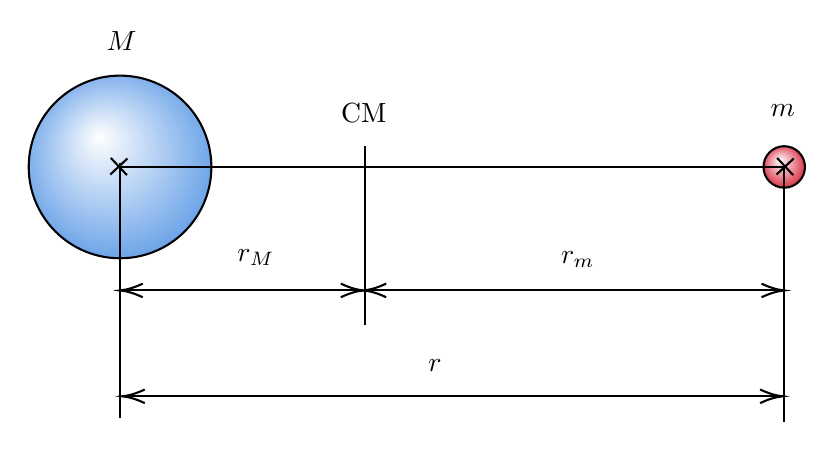
\begin{tikzpicture}[x=0.75pt,y=0.75pt,yscale=-1,xscale=1]
		\tikzset {_avpxot3y9/.code = {\pgfsetadditionalshadetransform{ \pgftransformshift{\pgfpoint{89.1 bp } { -128.7 bp }  }  \pgftransformscale{1.32 }  }}}
		\pgfdeclareradialshading{_xpm1kmh76}{\pgfpoint{-72bp}{104bp}}{rgb(0bp)=(1,1,1);
		rgb(0bp)=(1,1,1);
		rgb(25bp)=(0.29,0.56,0.89);
		rgb(400bp)=(0.29,0.56,0.89)}
		
		% Gradient Info
		  
		\tikzset {_mf7op4gb3/.code = {\pgfsetadditionalshadetransform{ \pgftransformshift{\pgfpoint{89.1 bp } { -128.7 bp }  }  \pgftransformscale{1.32 }  }}}
		\pgfdeclareradialshading{_7l3xxvw04}{\pgfpoint{-72bp}{104bp}}{rgb(0bp)=(1,1,1);
		rgb(0bp)=(1,1,1);
		rgb(25bp)=(0.82,0.01,0.11);
		rgb(400bp)=(0.82,0.01,0.11)}
		%uncomment if require: \path (0,638); %set diagram left start at 0, and has height of 638
		
		%Shape: Circle [id:dp016448649369496637] 
		\path  [shading=_xpm1kmh76,_avpxot3y9] (130,125) .. controls (130,100.7) and (149.7,81) .. (174,81) .. controls (198.3,81) and (218,100.7) .. (218,125) .. controls (218,149.3) and (198.3,169) .. (174,169) .. controls (149.7,169) and (130,149.3) .. (130,125) -- cycle ; % for fading 
		 \draw   (130,125) .. controls (130,100.7) and (149.7,81) .. (174,81) .. controls (198.3,81) and (218,100.7) .. (218,125) .. controls (218,149.3) and (198.3,169) .. (174,169) .. controls (149.7,169) and (130,149.3) .. (130,125) -- cycle ; % for border 
		
		%Shape: Circle [id:dp7274339138670711] 
		\path  [shading=_7l3xxvw04,_mf7op4gb3] (484,125) .. controls (484,119.48) and (488.48,115) .. (494,115) .. controls (499.52,115) and (504,119.48) .. (504,125) .. controls (504,130.52) and (499.52,135) .. (494,135) .. controls (488.48,135) and (484,130.52) .. (484,125) -- cycle ; % for fading 
		 \draw   (484,125) .. controls (484,119.48) and (488.48,115) .. (494,115) .. controls (499.52,115) and (504,119.48) .. (504,125) .. controls (504,130.52) and (499.52,135) .. (494,135) .. controls (488.48,135) and (484,130.52) .. (484,125) -- cycle ; % for border 
		
		%Straight Lines [id:da026213211076040466] 
		\draw    (174,125) -- (291.3,125) ;
		\draw   (169.57,120.66) -- (177.31,128.93)(177.57,120.93) -- (169.31,128.66) ;
		\draw   (490.57,120.66) -- (498.31,128.93)(498.57,120.93) -- (490.31,128.66) ;
		%Straight Lines [id:da817744626054181] 
		\draw    (292,115) -- (292,201) ;
		%Straight Lines [id:da4380801733856945] 
		\draw    (291.3,125) -- (494,125) ;
		%Straight Lines [id:da8072830390480916] 
		\draw    (174,123) -- (174,246) ;
		%Straight Lines [id:da3003472490526946] 
		\draw    (494,125) -- (494,248) ;
		%Straight Lines [id:da30481138054769463] 
		\draw    (176,184.5) -- (289.3,184.5) ;
		\draw [shift={(291.3,184.5)}, rotate = 180] [color={rgb, 255:red, 0; green, 0; blue, 0 }  ][line width=0.75]    (10.93,-3.29) .. controls (6.95,-1.4) and (3.31,-0.3) .. (0,0) .. controls (3.31,0.3) and (6.95,1.4) .. (10.93,3.29)   ;
		\draw [shift={(174,184.5)}, rotate = 0] [color={rgb, 255:red, 0; green, 0; blue, 0 }  ][line width=0.75]    (10.93,-3.29) .. controls (6.95,-1.4) and (3.31,-0.3) .. (0,0) .. controls (3.31,0.3) and (6.95,1.4) .. (10.93,3.29)   ;
		%Straight Lines [id:da41138326347220144] 
		\draw    (293.3,184.5) -- (492,184.5) ;
		\draw [shift={(494,184.5)}, rotate = 180] [color={rgb, 255:red, 0; green, 0; blue, 0 }  ][line width=0.75]    (10.93,-3.29) .. controls (6.95,-1.4) and (3.31,-0.3) .. (0,0) .. controls (3.31,0.3) and (6.95,1.4) .. (10.93,3.29)   ;
		\draw [shift={(291.3,184.5)}, rotate = 0] [color={rgb, 255:red, 0; green, 0; blue, 0 }  ][line width=0.75]    (10.93,-3.29) .. controls (6.95,-1.4) and (3.31,-0.3) .. (0,0) .. controls (3.31,0.3) and (6.95,1.4) .. (10.93,3.29)   ;
		%Straight Lines [id:da3372137861535347] 
		\draw    (177,235.5) -- (491.3,235.5) ;
		\draw [shift={(493.3,235.5)}, rotate = 180] [color={rgb, 255:red, 0; green, 0; blue, 0 }  ][line width=0.75]    (10.93,-3.29) .. controls (6.95,-1.4) and (3.31,-0.3) .. (0,0) .. controls (3.31,0.3) and (6.95,1.4) .. (10.93,3.29)   ;
		\draw [shift={(175,235.5)}, rotate = 0] [color={rgb, 255:red, 0; green, 0; blue, 0 }  ][line width=0.75]    (10.93,-3.29) .. controls (6.95,-1.4) and (3.31,-0.3) .. (0,0) .. controls (3.31,0.3) and (6.95,1.4) .. (10.93,3.29)   ;
		
		% Text Node
		\draw (166,58.4) node [anchor=north west][inner sep=0.75pt]    {$M$};
		% Text Node
		\draw (486,93.4) node [anchor=north west][inner sep=0.75pt]    {$m$};
		% Text Node
		\draw (229,163.4) node [anchor=north west][inner sep=0.75pt]    {$r_{M}$};
		% Text Node
		\draw (385,164.4) node [anchor=north west][inner sep=0.75pt]    {$r_{m}$};
		% Text Node
		\draw (321,216.4) node [anchor=north west][inner sep=0.75pt]    {$r$};
		% Text Node
		\draw (279,93) node [anchor=north west][inner sep=0.75pt]   [align=left] {CM};
		
		\end{tikzpicture}
		\vspace*{3mm}
		\caption[]{Binary system center of mass (profile view)}
	\end{figure}
	And let us have a look at circular orbits in the center of mass frame! 
	
	First we look at the forces acting on body $M$:
	
	The forces balance, so:
	
	We know that in the simple case of a circular orbit (circular kinematics):
	
	We insert this into the previous equation and we get after some algebra:
	
	What is $r_M$? From the definition of center of mass we know that (\SeeChapter{see section Classical Mechanics page \pageref{center of mass}}):
	
	We plug $r_M$ into our equation and now we get:
	
	or after rearranging terms:
	
	So we can use this 3rd Kepler's law to determine the total mass a binary pair if we know the period $T$!!! As the star masses are well estimated using the HR diagram we better understand how astronomers estimate orbiting planet mass knowing the period (in fact they also use the luminosity variation). In fact it is not as simple as there is no reason why we should be looking directly onto the orbital plane of the binary system. In other words, the apparent orbit is almost never the true orbit (which is what we need to do the calculation). 
	\begin{figure}[H]
		\centering
		\includegraphics[width=0.8\textwidth]{img/cosmology/barycentre_solar_system.png}
		\vspace*{3mm}
		\caption[Moving barycentre of the solar system]{In case of a $n$-body system (here the solar system) even the center of mass moves (source: Wikipedia)} 
	\end{figure}
	
	This interlude performed, let us come back on our Newton's gravitation law:
	
	From the law of gravitation, we can find back Kepler's law. Besides, we have already done it for the second and third law of Kepler, since it is these that we used to get this latter relation (however it's a little bit the snake eating its tail...).
	
	In vector notation we have therefore:
	
	Identically to the electric field (\SeeChapter{see section Electrostatics page \pageref{electric force}}), we can develop:
	
	As the electric field is derived from an electric potential, identically, the gravitational field derived from a gravitational potential\index{gravitation potential}\label{gravitation potential}. By performing exactly the same development as in  our study of electromagnetism for the first Maxwell equation (\SeeChapter{see section Electrodynamics page \pageref{first maxwell equation}}), we prove that:
	
	where $\varphi$ is the "\NewTerm{gravitational potential}\index{gravitational potential}" that varies inversely with the relative distance of the body (this confirms what we had proved in our study of Noether's theorem in the section on Principles) and is therefore equal to:
	
	\begin{tcolorbox}[title=Remark,arc=10pt,breakable,drop lifted shadow,
  skin=enhanced,
  skin first is subskin of={enhancedfirst}{arc=10pt,no shadow},
  skin middle is subskin of={enhancedmiddle}{arc=10pt,no shadow},
  skin last is subskin of={enhancedlast}{drop lifted shadow}]
	We often encounter this potential in the section of General Relativity. It is therefore appropriate to remember it if possible!
	\end{tcolorbox}	
	Notation which obviously implies the following relation:
	
	\begin{tcolorbox}[title=Remark,arc=10pt,breakable,drop lifted shadow,
  skin=enhanced,
  skin first is subskin of={enhancedfirst}{arc=10pt,no shadow},
  skin middle is subskin of={enhancedmiddle}{arc=10pt,no shadow},
  skin last is subskin of={enhancedlast}{drop lifted shadow}]
	Obviously in the absence of field, we have $\varphi=c^{te}$ and therefore $\vec{a}$  will be zero.
	\end{tcolorbox}
	As in the section of Electromagnetism, again, we prove as we did for the first Maxwell equation:
	
	If we express this equation in terms of a gravitational potential $\varphi$ (also often denoted by the letter $U$ as in Electrostatic...), we get:
	
	that we write more aesthetically with the scalar Laplacian operator (\SeeChapter{see section Vector Calculus page \pageref{scalar laplacian}}):
	
	which is nothing else than the "\NewTerm{Newton-Poisson equation}\index{Newton-Poisson equation}\label{newton-poisson equation}" that we will  also meet again in our study of General Relativity (it has an important place for validation reasons of Einstein's Gravitation theory)!
	
	This equation means that the Newtonian gravitational theory can be resume to say that the gravitational field is described by a single potential $\varphi$ generated by the volume mass density and determining the acceleration of a test particle immersed in the outfield $\varphi$.
	
	With Newton’s important achievements - building, of course, on the work of the great thinkers who preceded him - civilization reached an extremely high level of knowledge about the universe. Newtonian mechanics and also the optics, astronomy, and mathematics to which Newton contributed were immensely valuable in helping us gain an understanding of the vast and complicated physical world around us. The progress made by Newton and others allowed us to see clearly how planets move and how the force of gravity operates in nature. Newton’s theory of gravity is so profound and so all-encompassing that its laws govern everything from the fall of apples to the ground to the orbiting of the Earth by the Moon; from the revolutions of the planets around the Sun to the actions of springs and the trajectories of cannonballs; from the behaviour of billiard balls to the energy of an accelerating car. Newtonian mechanics explains the world to a stunningly accurate degree. In the 120th century (holocene calendar), Einstein would refine Newton’s theories to account for instances where the speed of light is approached or very great mass is involved. But for the time, Newton’s achievements truly opened a new world for physical science. In the following two centuries, science would consolidate its gains, and the church (and religions in general) would have to retreat from its position as the source of truth about how the world works.
	
	Let's have a little bit fun now with the Newton's gravitation equation to get some interesting and curious results:
	
	\subsubsection{Gaussian Formulation of Newtonian Gravity}
	As we have just mentioned it and proved in the section of Electrodynamics, an alternative formulation of Newtonian gravity is: Gauss’s Law for gravity. It states that the acceleration $\vec{a}$ due to gravity of a mass $m$ (not necessarily a point mass) is given by:
	
	where the $-$ sign we have it's purpose of guarantee a positive scalar acceleration.
	
	For example, let's use Gauss's law to find the acceleration $a$ due to the gravity of a point mass $m$.

	We begin with a point mass $m$ sitting in space. We now need to construct an imaginary closed surface $S$ surrounding $m$. While in theory any surface would do, we should pick a surface that will make the integral easy to evaluate. Such a surface should have these properties:
	\begin{enumerate}
		\item[P1.] The gravitational acceleration $\vec{a}$ should be either perpendicular or parallel to $S$ everywhere.

		\item[P2.] The gravitational acceleration $\vec{a}$ should have the same value everywhere on $S$ (or it may be zero on some parts of $S$).

		\item[P3.] The surface $S$ should pass through the point at which you wish to calculate the acceleration due to gravity.
	\end{enumerate}
	If we can find a surface $S$ that has these properties, the integral will be very simple to evaluate. For the point mass, we will choose $S$ to be a sphere of radius $r$ centered on mass $m$. Since we know $\vec{a}$ points radially inward toward mass $m$, it is clear that $g$ will be perpendicular to $S$ everywhere. Also, by symmetry, it is not hard to see that $\vec{a}$ will have the same value everywhere on $S$. 

	Having chosen a surface $S$, let us now apply Gauss’s law for gravity. The law states that for recall that:
	
	Now everywhere on the sphere $\mathcal{S}^2$, we have $\vec{a}\circ\vec{n}=-g$ (since $\vec{a}$ and $n$ are anti-parallel $g$ points inward, and $n$ points outward). Since $g$ is a constant for a perfect sphere, the previous relation becomes:
	
	Now the integral is very simple: it is just $\mathrm{d}S$ integrated over the surface of a sphere, so it's just the area of a sphere (\SeeChapter{see section Geometric Shapes page \pageref{sphere}}):
	
	or (cancelling $-4\pi$ on both sides):
	
	and it's in agreement with the Gravitational Newton law! This result suggests that the gravity of a solid spherical ball to an exterior object can be simplified as that of a point mass in the center of the ball with the same mass!!!
	
	Our planet isn't however a perfect sphere, it isn't also egg shaped, but it's a geoid and it's gravity field is even more complex that it's inside is not homogeneous. This gravity map from the GRACE satellite shows the variation of the gravitational field across Earth’s surface; red indicates higher gravitational field strength and blue lower:
	\begin{figure}[H]
		\centering
		\includegraphics[scale=2.6]{img/cosmology/grace_gravity_map.jpg}
		\caption{Gravitational field across Earth’s surface}
	\end{figure}
	The place with the lowest gravitational field strength is Mexico City (0.28\% below average) helped by it's elevation, more than two thousand metres above sea level. The highest gravitational field strength is found in Helsinki (0.13\% above average).
	
	So the Flat-Earthers and some believers (following some holy books that we will not mention here) have to explain why everywhere in the World they can measure a falling object which acceleration corresponds to an approximately spherical Earth if that latter is flat...

	As Flat-Earther sometimes challenge physicists to prove that the Newton law is not the same for a flat Earth (I was also challenged once... and this was a very bad idea from my opponent) here is the proof!
	\begin{figure}[H]
		\centering
		\includegraphics[scale=0.7]{img/cosmology/flat_earth.jpg}
		\caption[]{Schematic idea of a flat planet like... Earth......}
	\end{figure}
	In this case, the appropriate Gaussian surface $S$ is a "pillbox" shape - a short cylinder whose flat faces - (of area $A$) are parallel to the plane of mass. In this case, everywhere along the curved surface of $S$, the gravitational acceleration $\vec{a}$ is perpendicular to the outward normal unit vector $\vec{n}$, so the curved sides of $S$ contribute nothing to the integral. Only the flat ends of the pillbox-shaped surface S contribute to the integral. On each end, $\vec{a}$ is anti-parallel to $\vec{n}$, so $\vec{a}\circ\vec{n}=-g$ on the ends.
	
	Now apply Gauss's law to this situation:
	
	Here the integral needs only to be evaluated over the two flat ends of $S$. Since $\vec{a}\circ\vec{n}=-g$, we can bring $-g$ outside the integral to get:
	
	The integral in this case is just the area of the two ends of the cylinder, $2A$ (one circle of area $A$ from each end). This gives:
	
	Now let us look at the right-hand side of this equation. The mass $m$ is the total amount of mass enclosed by surface $S$. Surface $S$ is sort of a "cookie cutter" that punches a circle of area $A$ out of the plane. The mass
enclosed by $S$ is a circle of area $A$ and surfacic density $\sigma$, so it has mass $\sigma A$. Then the previous relation becomes:
	
	Note that this is a constant: the acceleration due to gravity of an infinite plane of mass $m$ is independent of the distance from the plane...! We will detail the much more complex case of a finite homogeneous disc further below at page \pageref{gravitation disc}.

	So Flat-Earther have difficulties to only difficulties to explain this but also are not able to find the corresponding value of $g$ in their laboratory or home garage...

	\subsubsection{Shell Theorem}\label{shell theorem}
	The shell theorem gives gravitational simplifications that can be applied to objects inside or outside a spherically symmetrical body. This theorem has particular application to astronomy.

	Isaac Newton proved the shell theorem and stated that:
	\begin{enumerate}
		\item A spherically symmetric body affects external objects gravitationally as though all of its mass were concentrated at a point at its center.
		\item If the body is a spherically symmetric shell (i.e., a hollow ball), no net gravitational force is exerted by the shell on any object inside, regardless of the object's location within the shell.
	\end{enumerate}
	A corollary is that, and we will prove it, that inside a solid sphere of constant density, the gravitational force varies linearly with distance from the center, becoming zero by symmetry at the center of mass.
	
	Given an object located outside of the Earth and $r$ is the distance of the object to the center of the Earth, we have:
	
	it comes:
	
	If the object is placed at the surface of the Earth or radius $R$, we have ($r=R$):
	
	From the two previous relations it comes therefore:
	
	At the surface we have then well (we expected this result...):
	
	Now, if the object is located inside the Earth by denoting the distance from the center by the letter $r$ and the central mass by $M'$, we have:
	
	Let us introduce the density $\rho$ that we will assume equal everywhere:
	
	By combining these last four relations, we get:
	
	\begin{figure}[H]
		\centering
		\begin{tikzpicture}[x=0.75pt,y=0.75pt,yscale=-1,xscale=1]
		%uncomment if require: \path (0,1046); %set diagram left start at 0, and has height of 1046
		
		%Shape: Axis 2D [id:dp6655532431005151] 
		\draw  (132.5,397.2) -- (566.5,397.2)(153.5,160.6) -- (153.5,423.2) (559.5,392.2) -- (566.5,397.2) -- (559.5,402.2) (148.5,167.6) -- (153.5,160.6) -- (158.5,167.6)  ;
		%Straight Lines [id:da023016570552313542] 
		\draw [color={rgb, 255:red, 155; green, 155; blue, 155 }  ,draw opacity=1 ][line width=0.75]  [dash pattern={on 4.5pt off 4.5pt}]  (148.5,246.6) -- (258.5,246.6) ;
		%Straight Lines [id:da029326202491650966] 
		\draw [color={rgb, 255:red, 155; green, 155; blue, 155 }  ,draw opacity=1 ][line width=0.75]  [dash pattern={on 4.5pt off 4.5pt}]  (258.5,246.6) -- (258.5,404.2) ;
		%Straight Lines [id:da842281898763948] 
		\draw [line width=1.5]    (258.5,246.6) -- (153.5,397.2) ;
		%Curve Lines [id:da8776253664329956] 
		\draw [line width=1.5]    (258.5,246.6) .. controls (278.5,353.2) and (412.5,390.2) .. (543.5,392.2) ;
		%Straight Lines [id:da7891301311539922] 
		\draw    (141.5,305.2) -- (186.5,338.2) ;
		\draw [shift={(186.5,338.2)}, rotate = 36.25] [color={rgb, 255:red, 0; green, 0; blue, 0 }  ][fill={rgb, 255:red, 0; green, 0; blue, 0 }  ][line width=0.75]      (0, 0) circle [x radius= 3.35, y radius= 3.35]   ;
		%Straight Lines [id:da2562306761333266] 
		\draw    (354.5,271.2) -- (299.5,311.2) ;
		\draw [shift={(299.5,311.2)}, rotate = 143.97] [color={rgb, 255:red, 0; green, 0; blue, 0 }  ][fill={rgb, 255:red, 0; green, 0; blue, 0 }  ][line width=0.75]      (0, 0) circle [x radius= 3.35, y radius= 3.35]   ;
		
		% Text Node
		\draw (138,400.6) node [anchor=north west][inner sep=0.75pt]   [align=left] {O};
		% Text Node
		\draw (186,406.6) node [anchor=north west][inner sep=0.75pt]   [align=left] {initial};
		% Text Node
		\draw (289,406.6) node [anchor=north west][inner sep=0.75pt]   [align=left] {external};
		% Text Node
		\draw (572,398) node [anchor=north west][inner sep=0.75pt]    {$r$};
		% Text Node
		\draw (115,154) node [anchor=north west][inner sep=0.75pt]    {$g( r)$};
		% Text Node
		\draw (250,409) node [anchor=north west][inner sep=0.75pt]    {$R$};
		% Text Node
		\draw (129,235) node [anchor=north west][inner sep=0.75pt]    {$g_{0}$};
		% Text Node
		\draw (60,278) node [anchor=north west][inner sep=0.75pt]    {$g( r) =g_{0}\dfrac{r}{R}$};
		% Text Node
		\draw (362,238) node [anchor=north west][inner sep=0.75pt]    {$g( r) =g_{0}\left(\dfrac{R}{r}\right)^{2}$};
		
		\end{tikzpicture}
		\vspace*{3mm}
		\caption{Internal/External gravitational acceleration profile of a mass body}
	\end{figure}

	For many people this result is quite counter-intuitive (do a little survey around you, you'll see).
	
	\begin{tcolorbox}[title=Remark,arc=10pt,breakable,drop lifted shadow,
  skin=enhanced,
  skin first is subskin of={enhancedfirst}{arc=10pt,no shadow},
  skin middle is subskin of={enhancedmiddle}{arc=10pt,no shadow},
  skin last is subskin of={enhancedlast}{drop lifted shadow}]
	In addition to gravity, the shell theorem can also be used to describe the electric field generated by a static spherically symmetric charge density, or similarly for any other phenomenon that follows an inverse square law. The derivations below focus on gravity, but the results can easily be generalized to the electrostatic force. 
	\end{tcolorbox}
	
	\subsubsection{Orbital speed}
	We will prove now an obvious property of orbits that will be useful to us later to study of what seem to be an anomaly with structure of the size of galaxies.
	
	The orbital speed of a body, generally a planet, a natural satellite, an artificial satellite, or a multiple star, is the speed at which it orbits around the barycenter of a system, usually around a more massive body. It can be used to refer to either the mean orbital speed, i.e. the average speed as it completes an orbit, or the speed at a particular point in its orbit such as perihelion.
	
	We have proved just earlier above the origin of Newton's law. For planets thus considered as physical points in stable circular orbit, there must be balance between centrifugal and gravitational force. So we have:
	
	where we easily deduce:
	
	Which is approximately in good agreement with the experimental measurements as shown in the figure below:
	\begin{figure}[H]
		\centering
		\includegraphics[scale=0.55]{img/cosmology/orbital_speed.jpg}	
		\caption{Orbital speed characteristic curve}
	\end{figure}
	But as we will prove it in the section of Aerospace Engineering (Vis-Viva equation at page \pageref{vis-viva equation}) in a more general case that orbital speed is given by:
	
	\begin{tcolorbox}[colframe=black,colback=white,sharp corners,breakable]
	\textbf{{\Large \ding{45}}Example:}\\\\
	Let us consider the case of Earth and Sun system: we have therefore:
	
	Let us consider now two case:
	\begin{itemize}
		\item The aphelion $r:=a_{\earth}$, then we have:
		
		\item The perihelion $r:=p_{\earth}=$, then we have:
		
	\end{itemize}
	In its elliptical orbit Earth orbital speed increases and decreases periodically. So the tangential acceleration changes all the time. In perihelion the speed as calculated above is about $29.82\;[\text{km}\cdot\text{s}^{-1}]$ and in aphelion about $29.74\;[\text{km}\cdot\text{s}^{-1}]$. To find the order of magnitude of the tang. acc. we can take simply $a=\mathrm{d} v / \mathrm{d} t$ knowing that between the aphelion and perihelion we have a duration of half a year, ie $15,779,000\;[\text{s}]$, hence:
	
	Hence the fact that we can't we with our Human sense Earth's movement on orbit!
	\end{tcolorbox}
	
	\subsubsection{Gravitational field of a homogeneous disc}\label{gravitation disc}
	Despite well-established results about the shape of the Earth, which is a geoid the naïve conception of the flat Earth\index{flat Earth} in some cases survives in adults' minds, especially by those indoctrinated by the holy books of all the abrahamic religions that explicitly claim the Earth is flat (and obviously the abrahamic deity could not be wrong... so if you have the faith you have to reject the scientific evidence). So we will prove here that such a shape for the Earth would have huge consequences on the gravitational field of the latter. 
	
	However it is not the only reason why we will derive that field! The main reason is that is also useful to understand how is shaped the gravitational field of disc shaped galaxies that can in first approximation be considered as homogeneous disc of matter and makes then more clear why the speed of stars orbiting the center of galaxies are faster when go away from the center rather than slower (as it is case if all the mass is located at the center of the galaxy). Also the result applies identically for the electric field of a homogeneous charged disc (that may be useful too)!
	
	To describe a flat Earth (or a flat disc shaped galaxy), we use a simple model of a thin disc with a uniformly distributed mass. This approach allows for rather simple calculations to demonstrate what would the gravitational field of such a system be!
	
	\begin{tcolorbox}[enhanced,title=Remark,colframe=black,arc=10pt,drop lifted shadow,after skip=15pt plus 2pt]
	All the derivations, figures that follow are mostly a copy/paste with a slight adaptation of the paper \cite{kuzii2019gravitation}.
	\end{tcolorbox}
	
	A point mass $M$ located at the origin creates at a point given by the radius-vector $\vec{r}$ a gravitational field with the potential:
	
	where $G$ is the gravitational constant. The respective gravitational field strength $\Gamma$ is:
	
	and hence the attraction force between the mass $M$ and a mass $m$ located at $\vec{r}$ reads:
	
	which is the well-known Newton's law of gravitation. Note that the vector $r$ points from the mass $M$ to the mass $m$ while the force pulls the mass $m$ towards $M$, hence the minus sign.

	For a set of point masses $M_i$ located at points $\vec{r}_i$ the gravitational potential is:
	
	yielding in the continuous limit:
	
	where $\rho\left(\vec{r}\,'\right)$ is the density, or for surface distributions:
	
	where $\sigma\left(\vec{r}\,'\right)$ is the surface density.
	
	We will model a flat Earth by a disc of radius $R$ with a constant surface density $\sigma=c^{te}$. It is most convenient to consider this problem in the cylindrical coordinates $(r,\phi,z)$. Let the observer sit at a point $(r, 0, z)$ (the angle doesn't matter given the symmetry of the problem... so take $0$ for angle will very likely simplify calculations a bit), and the elementary area $\mathrm{d}S=r^{\prime} \mathrm{d}r^{\prime}\mathrm{d} \phi$ has the cylindrical coordinates $\left(r^{\prime}, \phi, 0\right)$ as visible below:
	\begin{figure}[H]
		\centering
		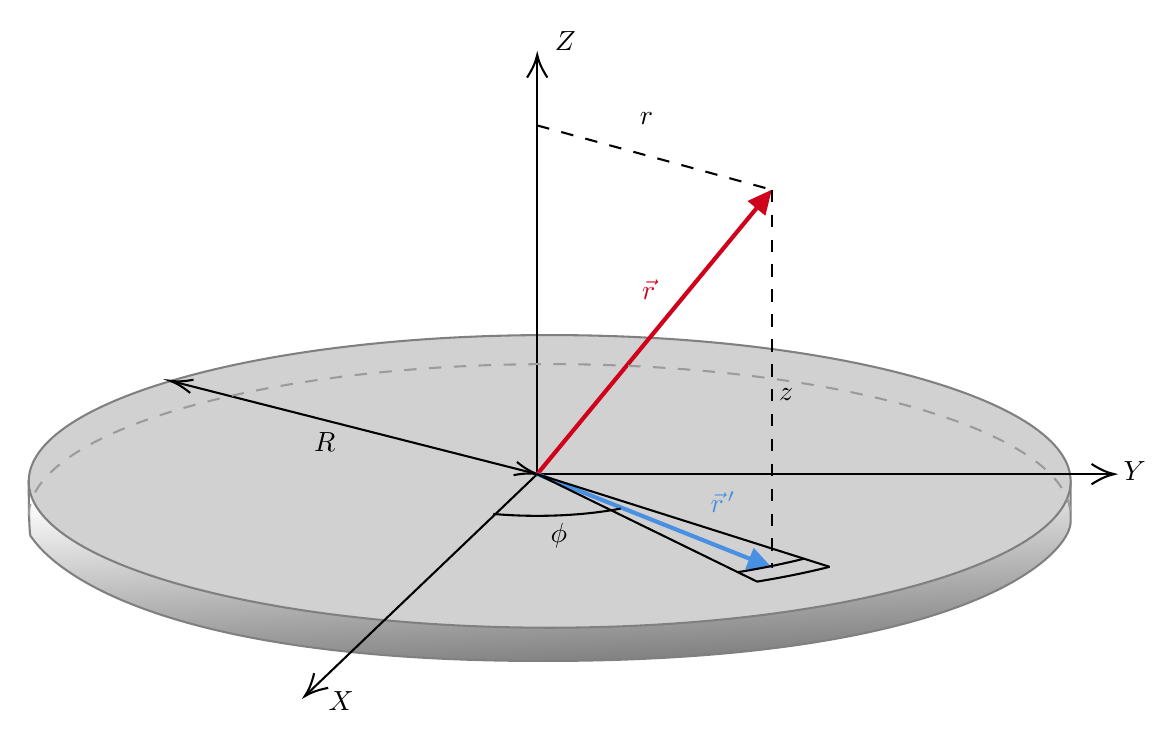
\begin{tikzpicture}[x=0.75pt,y=0.75pt,yscale=-1,xscale=1]
		%uncomment if require: \path (0,737); %set diagram left start at 0, and has height of 737
		
		% Gradient Info
		\tikzset {_9rexmvnsv/.code = {\pgfsetadditionalshadetransform{ \pgftransformshift{\pgfpoint{0 bp } { 0 bp }  }  \pgftransformrotate{-75 }  \pgftransformscale{2 }  }}}
		\pgfdeclarehorizontalshading{_49kkwghkw}{150bp}{rgb(0bp)=(1,1,1);
		rgb(37.5bp)=(1,1,1);
		rgb(62.5bp)=(0.5,0.5,0.5);
		rgb(100bp)=(0.5,0.5,0.5)}
		
		%Shape: Polygon Curved [id:ds5747989551289265] 
		\path  [shading=_49kkwghkw,_9rexmvnsv] (316,328) .. controls (528,329) and (576,276) .. (576,261) .. controls (576,246) and (575.86,241.71) .. (576,241.5) .. controls (576.14,241.29) and (74,240) .. (74,241.5) .. controls (74,243) and (74,268) .. (75,268) .. controls (76,268) and (104,327) .. (316,328) -- cycle ; % for fading 
		 \draw  [color={rgb, 255:red, 128; green, 128; blue, 128 }  ,draw opacity=1 ] (316,328) .. controls (528,329) and (576,276) .. (576,261) .. controls (576,246) and (575.86,241.71) .. (576,241.5) .. controls (576.14,241.29) and (74,240) .. (74,241.5) .. controls (74,243) and (74,268) .. (75,268) .. controls (76,268) and (104,327) .. (316,328) -- cycle ; % for border 
		
		%Shape: Ellipse [id:dp2037242141424942] 
		\draw  [color={rgb, 255:red, 128; green, 128; blue, 128 }  ,draw opacity=1 ][fill={rgb, 255:red, 209; green, 209; blue, 209 }  ,fill opacity=1 ] (74,241.5) .. controls (74,202.56) and (186.38,171) .. (325,171) .. controls (463.62,171) and (576,202.56) .. (576,241.5) .. controls (576,280.44) and (463.62,312) .. (325,312) .. controls (186.38,312) and (74,280.44) .. (74,241.5) -- cycle ;
		%Straight Lines [id:da51518988922686] 
		\draw    (319,238) -- (208.45,343.62) ;
		\draw [shift={(207,345)}, rotate = 316.31] [color={rgb, 255:red, 0; green, 0; blue, 0 }  ][line width=0.75]    (10.93,-4.9) .. controls (6.95,-2.3) and (3.31,-0.67) .. (0,0) .. controls (3.31,0.67) and (6.95,2.3) .. (10.93,4.9)   ;
		%Straight Lines [id:da6368785334025955] 
		\draw    (319,238) -- (595,238) ;
		\draw [shift={(597,238)}, rotate = 180] [color={rgb, 255:red, 0; green, 0; blue, 0 }  ][line width=0.75]    (10.93,-4.9) .. controls (6.95,-2.3) and (3.31,-0.67) .. (0,0) .. controls (3.31,0.67) and (6.95,2.3) .. (10.93,4.9)   ;
		%Straight Lines [id:da16944122837357956] 
		\draw    (319,238) -- (319,38) ;
		\draw [shift={(319,36)}, rotate = 90] [color={rgb, 255:red, 0; green, 0; blue, 0 }  ][line width=0.75]    (10.93,-4.9) .. controls (6.95,-2.3) and (3.31,-0.67) .. (0,0) .. controls (3.31,0.67) and (6.95,2.3) .. (10.93,4.9)   ;
		%Straight Lines [id:da13430832603493692] 
		\draw    (143.94,193.49) -- (317.06,237.51) ;
		\draw [shift={(319,238)}, rotate = 194.26] [color={rgb, 255:red, 0; green, 0; blue, 0 }  ][line width=0.75]    (10.93,-3.29) .. controls (6.95,-1.4) and (3.31,-0.3) .. (0,0) .. controls (3.31,0.3) and (6.95,1.4) .. (10.93,3.29)   ;
		\draw [shift={(142,193)}, rotate = 14.26] [color={rgb, 255:red, 0; green, 0; blue, 0 }  ][line width=0.75]    (10.93,-3.29) .. controls (6.95,-1.4) and (3.31,-0.3) .. (0,0) .. controls (3.31,0.3) and (6.95,1.4) .. (10.93,3.29)   ;
		%Straight Lines [id:da30172423533750337] 
		\draw [color={rgb, 255:red, 208; green, 2; blue, 27 }  ,draw opacity=1 ][line width=1.5]    (319,238) -- (429.45,104.09) ;
		\draw [shift={(432,101)}, rotate = 129.52] [fill={rgb, 255:red, 208; green, 2; blue, 27 }  ,fill opacity=1 ][line width=0.08]  [draw opacity=0] (11.61,-5.58) -- (0,0) -- (11.61,5.58) -- cycle    ;
		%Straight Lines [id:da8966745529128841] 
		\draw [color={rgb, 255:red, 0; green, 0; blue, 0 }  ,draw opacity=1 ] [dash pattern={on 4.5pt off 4.5pt}]  (319,70) -- (432,101) ;
		%Straight Lines [id:da004284464091390383] 
		\draw [color={rgb, 255:red, 0; green, 0; blue, 0 }  ,draw opacity=1 ] [dash pattern={on 4.5pt off 4.5pt}]  (432,101) -- (432,283) ;
		%Straight Lines [id:da8124163644547238] 
		\draw [color={rgb, 255:red, 74; green, 144; blue, 226 }  ,draw opacity=1 ][line width=1.5]    (319,238) -- (428.28,281.52) ;
		\draw [shift={(432,283)}, rotate = 201.71] [fill={rgb, 255:red, 74; green, 144; blue, 226 }  ,fill opacity=1 ][line width=0.08]  [draw opacity=0] (11.61,-5.58) -- (0,0) -- (11.61,5.58) -- cycle    ;
		%Shape: Arc [id:dp8071092245449203] 
		\draw  [draw opacity=0] (359.26,254.58) .. controls (347.8,256.79) and (333.94,258.09) .. (319,258.09) .. controls (311.62,258.09) and (304.5,257.77) .. (297.8,257.18) -- (319,238) -- cycle ; \draw   (359.26,254.58) .. controls (347.8,256.79) and (333.94,258.09) .. (319,258.09) .. controls (311.62,258.09) and (304.5,257.77) .. (297.8,257.18) ;  
		%Straight Lines [id:da19316964609474851] 
		\draw    (319,238) -- (424.92,289.78) ;
		%Straight Lines [id:da8590080184526963] 
		\draw    (319,238) -- (459.87,282.66) ;
		%Shape: Arc [id:dp4133768043367114] 
		\draw  [draw opacity=0] (447.52,278.74) .. controls (437.73,281.2) and (427.05,283.38) .. (415.64,285.24) -- (319,238) -- cycle ; \draw   (447.52,278.74) .. controls (437.73,281.2) and (427.05,283.38) .. (415.64,285.24) ;  
		%Shape: Arc [id:dp07952895871357635] 
		\draw  [draw opacity=0] (459.87,282.66) .. controls (449.14,285.35) and (437.44,287.74) .. (424.92,289.78) -- (319,238) -- cycle ; \draw   (459.87,282.66) .. controls (449.14,285.35) and (437.44,287.74) .. (424.92,289.78) ;  
		%Shape: Arc [id:dp0341543149528436] 
		\draw  [draw opacity=0][dash pattern={on 4.5pt off 4.5pt}] (74,258.25) .. controls (74,258.25) and (74,258.25) .. (74,258.25) .. controls (74,258.25) and (74,258.25) .. (74,258.25) .. controls (74,217.8) and (186.38,185) .. (325,185) .. controls (463.62,185) and (576,217.8) .. (576,258.25) -- (325,258.25) -- cycle ; \draw  [color={rgb, 255:red, 155; green, 155; blue, 155 }  ,draw opacity=1 ][dash pattern={on 4.5pt off 4.5pt}] (74,258.25) .. controls (74,258.25) and (74,258.25) .. (74,258.25) .. controls (74,258.25) and (74,258.25) .. (74,258.25) .. controls (74,217.8) and (186.38,185) .. (325,185) .. controls (463.62,185) and (576,217.8) .. (576,258.25) ;  
		
		% Text Node
		\draw (326,23.4) node [anchor=north west][inner sep=0.75pt]    {$Z$};
		% Text Node
		\draw (600,230.4) node [anchor=north west][inner sep=0.75pt]    {$Y$};
		% Text Node
		\draw (217,341.4) node [anchor=north west][inner sep=0.75pt]    {$X$};
		% Text Node
		\draw (210,216.4) node [anchor=north west][inner sep=0.75pt]    {$R$};
		% Text Node
		\draw (367,62.4) node [anchor=north west][inner sep=0.75pt]    {$r$};
		% Text Node
		\draw (434,195.4) node [anchor=north west][inner sep=0.75pt]    {$z$};
		% Text Node
		\draw (368,143) node [anchor=north west][inner sep=0.75pt]    {$\textcolor[rgb]{0.82,0.01,0.11}{\vec{r}}$};
		% Text Node
		\draw (401,245) node [anchor=north west][inner sep=0.75pt]    {$\textcolor[rgb]{0.29,0.56,0.89}{\vec{r}^{\,\prime}}$};
		% Text Node
		\draw (324,260) node [anchor=north west][inner sep=0.75pt]    {$\phi$};
		
		\end{tikzpicture}
		\vspace*{3mm}
		\caption[]{Frame of reference and coordinates of the problem}
	\end{figure}
	To calculate the distance $\|\vec{r}-\vec{r}\,'\|$, one can go back to the Cartesian coordinates, $\vec{r}=(x,y,z)=(r, 0, z)$ and $\vec{r}\,'=\left(r^{\prime} \cos(\phi), r^{\prime} \sin(\phi), 0\right)$, so that:
	
	Thus, the gravitational potential is:
	
	The integration of the above expression appears to be unexpectedly complicated. As far as we know, the result cannot be expressed in elementary functions.
	
	So first let us rewrite the integral as following:
	
	Let us write $x$ as $\frac{1}{2}(2 x-2 r \cos (\phi))+r \cos (\phi)$ and split:
	
	Applying linearity:
	
	Now we solve first:
	
	Substitute:
	
	Therefore:
	
	So we have the primitive:
	
	Now we focus on:
	
	First we complete the square:
	
	Let us do the following substitution:
	
	Hence:
	
	Substituting in the integral leads to:
	
	This is an usual primitive that we already know:
	
	Now we undo the substitution with:
	
	Therefore:
	
	So finally:
	
	If we simplify:
	
	Now remember that we want the integral with $x$ (i.e. $r'$) between $0$ and $R$. Therefore:
	
	The outer integration of this expression, over $\phi$, is not possible in elementary function as far as we know (excepted for the term $\sqrt{z^2+r^2}$ obviously!). We will instead expand it into Maclaurin series over $r$. 
	
	So let us denote:
	
	And do the Maclaurin expansion at the sixth order:
	
	The reader can get more terms or check the above result with Maple 4.00b with the following command:\\\\
	\texttt{>taylor(sqrt(z\string^2+r\string^2+R\string^2-2*R*r*cos(phi))-sqrt(z\string^2+r\string^2)+r*cos(phi)\\
	*(ln(R-r*cos(phi)+sqrt(z\string^2+r\string^2+R\string^2-2*R*r*cos(phi)))-ln(sqrt(r\string^2+z\string^2)\\
	-r*cos(phi))),r=0,5);}
	
	The integration of the first row above is obvious, for the others it's too boring to do that manually. The fastest solution is to use again Maple 4.00b integration function!
	
	Therefore we use first:\\\\
	\texttt{>readlib(coeftayl):\\
	>approx:=taylor(sqrt(z\string^2+r\string^2+R\string^2-2*R*r*cos(phi))-sqrt(z\string^2+r\string^2)+r*cos(phi)\\
	*(ln(R-r*cos(phi)+sqrt(z\string^2+r\string^2+R\string^2-2*R*r*cos(phi)))-ln(sqrt(r\string^2+z\string^2)\\
	-r*cos(phi))),r=0,5);\\\\}
	The first integral is obvious, we don't need Maple for it:
	
	For the second term we start using Maple:\\\\
	\texttt{>int(coeftayl(approx, r=0, 1),phi=0..2*Pi);}
	Which leads to:
	
	Similarly for the third term:\\\\
	\texttt{>int(coeftayl(approx, r=0, 2),phi=0..2*Pi);\\\\}
	Which leads to:
	
	Similarly for the fourth term:\\\\
	\texttt{>int(coeftayl(approx, r=0, 3),phi=0..2*Pi);\\\\}
	Which leads to:
	
	Similarly for the fifth term:\\\\
	\texttt{>int(coeftayl(approx, r=0, 4),phi=0..2*Pi);\\\\}
	Which leads to:
	
	So finally:
	
	As there is no angular dependence in re relation above, the field strength becomes:
	
	where:
	
	The components of the gravitational field strength are therefore:
	
	Not let us focus on what we may consider as the most interesting case: the field depending or $r$ at a high of $z=0$:
	
	From these expressions we can readily extract some qualitative information about the behavior of the gravitational field strength of the flat Earth.

	The radial component of the gravitational field increases as one moves from the center of the Earth (or from an homogeneous galaxy in the shape of a disc) towards its edge. This changes the magnitude of the field and its direction changes from perpendicular at the center to nearly horizontal at the edge. Therefore, a person tending towards the edge of a flat Earth would need to bend in order to remain in the vertical position. 
	\begin{figure}[H]
		\centering
		\includegraphics[scale=2.0]{img/cosmology/flat_earth_gravity_illustration.jpg}
		\caption[Qualitative picture showing the direction of the gravitational field of a flat Earth]{Qualitative picture showing the direction of\\
		 the gravitational field of a flat Earth (source: \cite{kuzii2019gravitation})}
	\end{figure}
	The series expansions we did earlier give reliable results only at $r \lesssim R / 2$. As one approaches the edge of the disc, $r \rightarrow R$, the gravitational field strength grows sharply:
	\begin{figure}[H]
		\centering
		\includegraphics[scale=0.8]{img/cosmology/gravitational_field_flat_disc.jpg}
		\caption[Exact vs Approximate solution of disc shaped Earth gravitational field]{Magnitude of the gravitational field strength at the surface ($z=0$) where\\ the red solid line corresponds to the calculations according to the series expansions\\  while the black dashed line is the exact result (source: \cite{kuzii2019gravitation})}
	\end{figure}
	
	\begin{tcolorbox}[enhanced,title=Remark,colframe=black,arc=10pt,drop lifted shadow,after skip=15pt plus 2pt]
	The reader has to keep in mind that the result we get above also applies for a non-rotating disc charged electro-statically in an homogeneous way!
	\end{tcolorbox}
	So what we can conclude from these results is that at the opposite of a central gravitational punctual force where the objects that orbits the central one have a speed that decrease proportionally to $1/R$, in the case of a homogeneous disc of matter it seems to be likely that as the radial gravitational force increase rather than decreasing, the orbital speed of objects inside the disc also increase the further we go from the center! We may also imagine (but that would need a rigorous mathematical derivation) that if the disc has a density that decrease slightly the further we go from the center, then things compensate and we may fall back in a in between solution, ie: a constant speed! That's obviously just speculation... but may explain the observed "galaxy rotation curve\index{galaxy rotation curve}":
	\begin{figure}[H]
		\centering
		\includegraphics[width=1.0\textwidth]{img/cosmology/rotational_curve_m33.jpg}
		\caption[Newtonian expected (with naive central force) vs Observed rotation curve of the M 33 galaxy]{Newtonian expected (with naive central force) vs Observed rotation curve of the M 33 galaxy (source: \cite{zasov2017dark})}
	\end{figure}
	Here are other galaxies rotation curves:
	\begin{figure}[H]
		\centering
		\includegraphics[width=1.0\textwidth]{img/cosmology/galaxies_rotation_curves.jpg}
		\caption[Different galaxies rotation curves]{Different galaxies rotation curves (source: \cite{zasov2017dark})}
	\end{figure}
	With the corresponding pictures of the different galaxies (obviously we didn't provide any picture of the MW/Milky Way galaxy as we don't have any external picture of it yet...):
	\begin{figure}[H]
		\centering
		\includegraphics[width=1.0\textwidth]{img/cosmology/galaxies_rotation_curves_photos.jpg}
	\end{figure}
	The reader can see in a very detailed way at page \pageref{andromeda m31 hd} how looks like the density of stars in a galaxy like M31, or online at the following url (if the web page still exist at the day the reader will try it...):
	\begin{center}
		\url{https://esahubble.org/images/heic1502a/zoomable/}
	\end{center}
	
	\subsubsection{Collision time of two objects at rest}
	Let us consider in an empty space (vacuum) two objects spherical objects $A,B$ of identical mass $m$ and diameter $d$ separated from a distance $D$ and at rest. We want to know after what time they will collide?
	
	We know that the acceleration is given by:
	
	Let us defined the distance between our two objects by:
	
	Therefore by symmetry:
	
	Let us multiple both side by $2\dot{r}$. We then have:
	
	This relation can also be seen as the result of the following relation:
	
	We can integrate both side relatively to the time $t$, hence:
	
	We have for initial condition:
	
	Hence we can easily determine that the constant is given by:
	
	Therefore:
	
	Taking the square root (the minus sign is just a matter of convention!):
	
	Inverted this give us:
	
	And what we want is obviously integrate the latter:
	
	Hence we are seeking for the primitive of:
	
	Let us do a clever change of variable:
	
	Therefore:
	
	By our change of variable we also have:
	
	Hence:
	
	Assuming:
	
	ie $d\ll D$. Then:
	
	Hence:
	
	Therefore (the $d$ has disappeared because remember we assumed $d\ll D$):
	
	For example for two apples of $100$ [g] at $1$ [meter] of each other, we get $\Delta t \cong 3 \times 10^5\; [\text{s}]\cong 3\;[\text{days}]$. Don't forget that if you want the final speed you just apply the relation derived earlier above:
	
	For apples weighing $100$ [g], $r=10$ [cm], dropped $1$ [m] apart, we get a speed of $5$ centimetres per hour.
	
	\subsubsection{Asteroids/Meteors impact velocity}
	We have proved in the section of Classical Mechanics that the escape velocity was given by (see page \pageref{escape velocity}):
	
	and was therefore independent of the mass $m$ of the ejected object. Obviously the same relation can be applied for an object of mass $m$ coming from an infinite far distance.
	
	For the entry velocity of an asteroid in Earth's atmosphere we can assume that the minimum speed of a colliding asteroid is given by the above escape velocity relation for an asteroid returning to the zero potential of the Earth's gravitational field (a numerical application gives ${11 \;[\text{km}\cdot \text{s}^{-1}]}$.

	In fact, their real entering velocity depends on their direction that will determine their relative speed to Earth (which is ${30  \;[\text{km}\cdot \text{s}^{-1}]}$) plus eventually that of the Sun (which is around ${200  \;[\text{km}\cdot \text{s}^{-1}]}$. We can also take into account the escape velocity of the Solar System that is around  ${200  \;[\text{km}\cdot \text{s}^{-1}]}$.

	The sum gives therefore a speed between ${11 \;[\text{km}\cdot \text{s}^{-1}]}$ (for the optimistic case....) and ${300\;[\text{km}\cdot \text{s}^{-1}]}$ (for the pessimistic case....) with a statistical peak that gives most observed entry at ${30 \;[\text{km}\cdot \text{s}^{-1}]}$.

	As we  will prove it in the section of Weather and Marine Engineering (see page \pageref{visual horizon}) at a height of $600$ [m] we can see at a distance of almost $80$ [km], then we better understand why it is a joke in some movies to see huge asteroids entering the Earth atmosphere with people looking at it during $10$-$15$ seconds... and waiting almost $1$ minute before it hits the ground... (this is type of observation available for meteors but not for asteroids coming from very far!!!).

	A good example is to see all the YouTube videos about the small Chelyabinsk meteor (having a diameter of only $20$ meters) that entered Earth's atmosphere over Russia on 15 February 12013\footnote{The reader can download the \textit{Meteor Data Center database} of the International Astronomic Union for free on the Internet to see that the days where meteors fall down on Earth is completely random. Some days have meteor showers and some others - not always the same - don't have any meteor shower recorded.} (holocene calendar) and that had a speed of only almost  $30 \;[\text{km}\cdot \text{s}^{-1}]$ and which trajectory was visible during almost $20$ seconds only with the human eyes (so imagine with a speed $10$ times faster...).
	\begin{figure}[H]
		\centering
		\includegraphics[scale=0.4]{img/cosmology/asteroids_comets.jpg}	
		\caption[All asteroids and comets visited by spacecrafts as of November 12010]{All asteroids and comets visited by spacecraft as of November 12010 (source: Montage by Emily Lakdawalla. Ida, Dactyl, Braille, Annefrank, Gaspra, Borrelly: NASA / JPL / Ted Stryk. Steins: ESA / OSIRIS team. Eros: NASA / JHUAPL. Itokawa: ISAS / JAXA / Emily Lakdawalla. Mathilde: NASA / JHUAPL / Ted Stryk. Lutetia: ESA / OSIRIS team / Emily Lakdawalla. Halley: Russian Academy of Sciences / Ted Stryk. Tempel 1, Hartley 2: NASA / JPL / UMD. Wild 2: NASA / JPL)}
	\end{figure}
	Statistical counts of Meteor shower as given by the Meteor Data Center Database\footnote{The huge majority of meteoric dust cannot be observed with actual technologies, so there are no daily available statistics that we can provide here on that specific topic.}:
	\begin{figure}[H]
		\centering
		\includegraphics[width=1.0\textwidth]{img/cosmology/meteor_shower_statistics.jpg}
	\end{figure}
	\subsubsection{Spherisation of Celestial Bodies}
	Thanks to Newton's law, we could answer to a lot of relevant questions in an approximated way and giving us results quite convincing.

	A first example is to ask ourself at what scale there is a transition in the domain of irregular shapes (comets, asteroids, moons, etc.) to the field of spheres (moons, planets and stars)? Why the moons of Mars, Phobos and Deimos, have a potato shape like while our Moon is roughly spherical. We will see below that this is due to the mass that is greater in the case of our Moon. Indeed, from a certain mass, arbitrary geometric shapes are not possible anymore.

	To address this study, we will first estimate the maximum height of a mountain on a planet. Mount Everest has an altitude of $8.8$ [km] while Mount Olympus on Mars has a height of $27$ [km]. Why such mountains can not exist on Earth?

	To take a simplistic approach, we will assume that a mountain must be in hydrostatic equilibrium. We know experimentally the pressure limit in such a rocks lattice beyond which the rocks begin to "melt" (given in tables): $P_{\text{lim}}\cong 3 \cdot 10^8\;\text{[Pa]}$.

	We know from our study of continuum mechanics (\SeeChapter{see section Continuum Mechanics page \pageref{fundamental theorem of hydrostatics}}) the pressure at the base of a mountain of height $h$ will be given in the hydrostatic approximation by:
	
	For the mountain to be stable, it is necessary that:
	For the mountain to be stable, it is necessary that:
	
	and therefore:
	
	Therefore:
	
	Assuming an average density of $\rho=3,000\;[\text{kg}\cdot \text{m}^{-3}]$ (continental crust of the Earth) we get:
	\begin{enumerate}
		\item Earth: $h_0\cong 10\; [\text{km}]$
		\item Mars: $h_0\cong 27\; [\text{km}]$
	\end{enumerate}
	What is remarkable as approximate result!!!

	To estimate the minimum size $r_m$ of a body where the spherical shape becomes predominant compared to the surface deformation (that is to say where gravity has taken over the inter-atomic forces), we will require the size $r_m$ to be greater than the maximum height of a mountain of height $h_0$. We also assume that the density $\rho$ remains constant through the celestial body. Taking again the relation:
	
	we have:
	
	hence:
	
	The limit $r_m$ can after be estimated by fixing $r=r_m=h_0$ therefore:
	
	obviously for $r\gg r_m$ we will be even closer to the spherical shape.

	\paragraph{Flattening of Celestial Bodies (rotational flattening)}\mbox{}\\\\\
	Because of the symmetry of the gravitational potential a star or a planet should have a perfectly spherical form starting a given size, as we have just proved it. Now, the fact is... that it is not so for and especially for telluric bodies!
	
	Because of the own rotation of the star or planet, a centrifugal term transforms the potential. This term depends on the latitude which explains the ellipsoidal shape of most observed celestial bodies.
	
	Let us recall that:
	
	where $R$ is the equatorial radius of the star or planet, acceleration to which we have to add the centrifugal acceleration at a given latitude radius $r$ (\SeeChapter{see section Classical Mechanics page \pageref{centrifugal acceleration}}):
	
	Therefore the total acceleration given by:
	
	explains why the Earth is flattened at the poles (or depending of the point of view stretched to the equator ...) and that more one empty planet rotates, the more it will be flattened at the poles.
	
	On Earth, the equatorial radius is of $6,379$ [km] while the polar radius is of $6,357$ [km]. The difference is $22$ [km]. The "\NewTerm{flattening}\index{flattening}" of a star or planet is sometimes defined as:
	
	thus the difference between the equatorial radius and polar radius divided by the equatorial radius.
	
	Although an ellipsoid of revolution is the best description for the shape of a planet:
	\begin{figure}[H]
		\centering
		\includegraphics[scale=1.4]{img/cosmology/earth_with_atmosphere.jpg}	
		\caption{Earth with its atmosphere and oceans}
	\end{figure}
	there are obviously imperfections between the model and the reality for some planets (in particular the terrestrial planets, satellites, and small rocky bodies). The geopotential of real celestial bodies can be shaped in a much more complicated way because of the influences of the visible inhomogeneities on the surface as evidenced by these satellite images of the Earth omitting the liquid parts of it (the deformations are amplified by a factor $100,000$ in the image below!):
	\begin{figure}[H]
		\centering
		\includegraphics[width=1.0\textwidth]{img/cosmology/earth_without_atmosphere.jpg}	
		\caption[Earth shape without its atmosphere and oceans]{Earth shape without its atmosphere and oceans (source: Wikipedia)}
	\end{figure}
	So the Earth is obviously not a sphere nor Ostrich egg shaped...
	
	The "\NewTerm{geoid}\index{geoid}" is a particular equipotential surface of the Earth's gravity field and serves as a reference for the determination of altitudes. We can imagine the geoid as being the mean sea level extended under the continents.
	
	Considered globally, the geoid deviates from a mathematical reference surface (a rotational ellipsoid) by $\pm 100$ meters at most.
	\begin{figure}[H]
		\centering
		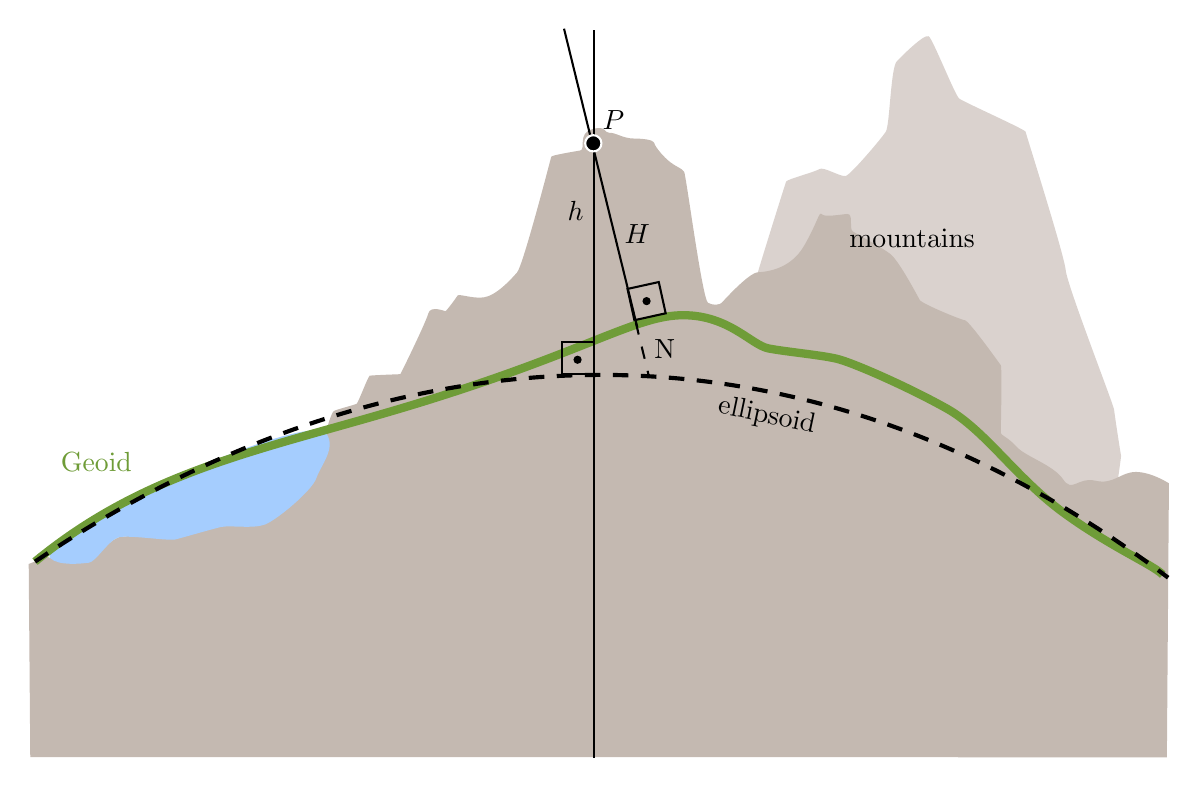
\begin{tikzpicture}[x=0.75pt,y=0.75pt,yscale=-1,xscale=1]
		%uncomment if require: \path (0,556); %set diagram left start at 0, and has height of 556
		
		%Shape: Polygon Curved [id:ds08160861567913269] 
		\draw  [draw opacity=0][fill={rgb, 255:red, 218; green, 210; blue, 206 }  ,fill opacity=1 ] (414.29,185.6) .. controls (414.62,184.06) and (427.41,143.01) .. (427.91,141.88) .. controls (428.42,140.76) and (441.92,137.23) .. (443.91,135.88) .. controls (445.91,134.54) and (454.18,139.78) .. (456.58,139.22) .. controls (458.99,138.65) and (473.96,120.95) .. (475.91,117.88) .. controls (477.86,114.82) and (478.21,87.01) .. (481.25,83.88) .. controls (484.29,80.76) and (494.58,70.55) .. (496.58,71.88) .. controls (498.58,73.22) and (509.23,100.27) .. (511.25,101.88) .. controls (513.26,103.5) and (543.06,116.76) .. (543.25,117.88) .. controls (543.44,119.01) and (561.88,177.11) .. (562.58,184.55) .. controls (563.28,192) and (585.65,249.25) .. (585.91,251.88) .. controls (586.18,254.52) and (589.04,273.14) .. (589.25,273.88) .. controls (589.46,274.63) and (583.91,311.22) .. (583.91,310.55) .. controls (583.91,309.88) and (400.58,238.55) .. (401.91,239.22) .. controls (403.25,239.88) and (413.95,187.14) .. (414.29,185.6) -- cycle ;
		%Shape: Polygon Curved [id:ds8443824368853541] 
		\draw  [draw opacity=0][fill={rgb, 255:red, 196; green, 185; blue, 177 }  ,fill opacity=1 ] (62.97,326.14) .. controls (62.97,326.14) and (71.91,322.55) .. (72.01,322.64) .. controls (72.11,322.73) and (78.41,325.42) .. (78.76,325.39) .. controls (79.11,325.36) and (94.86,322.69) .. (95.26,322.39) .. controls (95.67,322.1) and (102.39,314.41) .. (106.33,313.28) .. controls (110.26,312.14) and (132.55,312.33) .. (133.33,312.28) .. controls (134.1,312.23) and (154.96,306.36) .. (155.33,306.28) .. controls (155.7,306.2) and (167.76,306.5) .. (168.26,306.39) .. controls (168.76,306.29) and (176.76,304.89) .. (185.26,299.14) .. controls (193.76,293.39) and (196.33,289.03) .. (199.33,285.28) .. controls (202.33,281.53) and (206.77,263.8) .. (206.33,263.28) .. controls (205.89,262.76) and (208.74,253.19) .. (209.99,252.44) .. controls (211.24,251.69) and (220.24,249.44) .. (220.99,248.94) .. controls (221.74,248.44) and (226.49,235.69) .. (227.24,235.44) .. controls (227.99,235.19) and (241.81,234.71) .. (241.99,234.69) .. controls (242.17,234.66) and (254.49,209.44) .. (255.49,205.44) .. controls (256.49,201.44) and (263.33,204.32) .. (263.75,204.34) .. controls (264.17,204.35) and (268.74,198.19) .. (269.49,196.94) .. controls (270.24,195.69) and (276.49,198.44) .. (282.24,197.69) .. controls (287.99,196.94) and (295.24,189.19) .. (298.24,185.69) .. controls (301.24,182.19) and (314.49,130.66) .. (314.74,129.91) .. controls (314.99,129.16) and (325.99,127.41) .. (328.74,126.91) .. controls (331.49,126.41) and (327.24,118.66) .. (334.49,116.66) .. controls (341.74,114.66) and (339.99,118.66) .. (342.74,118.41) .. controls (345.49,118.16) and (349.4,121.16) .. (354.49,121.16) .. controls (359.58,121.16) and (363.99,121.91) .. (364.24,123.16) .. controls (364.49,124.41) and (367.25,128.41) .. (370.99,131.66) .. controls (374.73,134.92) and (377.75,135.41) .. (378.74,137.16) .. controls (379.73,138.92) and (387.54,198.85) .. (390.29,200.35) .. controls (393.04,201.85) and (396.04,201.1) .. (396.79,200.35) .. controls (397.54,199.6) and (409.79,185.85) .. (414.29,185.6) .. controls (418.79,185.35) and (430.04,184.1) .. (436.54,172.85) .. controls (443.04,161.6) and (443.79,155.98) .. (445.04,157.6) .. controls (446.29,159.21) and (454.04,157.76) .. (457.29,157.51) .. controls (460.54,157.26) and (458.04,164.71) .. (460.04,165.96) .. controls (462.04,167.21) and (473.79,173.51) .. (478.04,176.76) .. controls (482.29,180.01) and (491.29,197.23) .. (492.29,198.98) .. controls (493.29,200.73) and (512.04,208.48) .. (514.04,208.73) .. controls (516.04,208.98) and (530.54,229.35) .. (531.29,230.35) .. controls (532.04,231.35) and (531.29,262.01) .. (531.29,263.01) .. controls (531.29,264.01) and (535.04,265.26) .. (539.04,269.76) .. controls (543.04,274.26) and (556.79,278.55) .. (561.29,285.3) .. controls (565.79,292.05) and (568.29,284.05) .. (577.04,286.05) .. controls (585.79,288.05) and (589.04,281.73) .. (596.54,281.8) .. controls (604.03,281.88) and (612.33,287.28) .. (612.33,287.28) .. controls (612.33,287.28) and (611.33,419.28) .. (611.33,419.28) .. controls (611.33,419.28) and (63.72,419.14) .. (63.72,419.14) .. controls (63.72,419.14) and (62.97,326.14) .. (62.97,326.14) -- cycle ;
		%Shape: Polygon Curved [id:ds31108513470420984] 
		\draw  [draw opacity=0][fill={rgb, 255:red, 165; green, 205; blue, 254 }  ,fill opacity=1 ] (127.19,287.53) .. controls (153.19,274.53) and (201.33,256.28) .. (206.33,263.28) .. controls (211.33,270.28) and (203.59,278.73) .. (201.59,284.73) .. controls (199.59,290.73) and (182.53,304.94) .. (176.79,307.13) .. controls (171.04,309.32) and (159.93,307.35) .. (155.59,308.33) .. controls (151.24,309.32) and (136.79,313.55) .. (133.59,314.33) .. controls (130.38,315.11) and (111.12,312.06) .. (106.33,313.28) .. controls (101.53,314.5) and (95.33,325.16) .. (91.99,325.53) .. controls (88.64,325.9) and (77.33,327.28) .. (73.33,323.28) .. controls (69.33,319.28) and (101.19,300.53) .. (127.19,287.53) -- cycle ;
		%Curve Lines [id:da517087403035692] 
		\draw [color={rgb, 255:red, 111; green, 156; blue, 56 }  ,draw opacity=1 ][line width=3]    (66,325) .. controls (123.32,277.87) and (182.33,270.28) .. (258.33,246.28) .. controls (334.33,222.28) and (356.33,206.28) .. (378.33,206.28) .. controls (400.33,206.28) and (411.2,220.7) .. (419.33,222.28) .. controls (427.45,223.86) and (444.57,225.43) .. (452.33,227.28) .. controls (460.08,229.13) and (486.9,240.94) .. (505.33,251.28) .. controls (523.76,261.62) and (538.77,284.79) .. (561.33,301.28) .. controls (583.88,317.77) and (604.35,326.33) .. (609.33,331.28) ;
		%Curve Lines [id:da38619782967143923] 
		\draw [line width=1.5]  [dash pattern={on 5.63pt off 4.5pt}]  (66,325) .. controls (226.39,216.73) and (423.95,191.13) .. (611.95,332.73) ;
		%Shape: Square [id:dp7819673655232431] 
		\draw   (319.7,219.03) -- (335.13,219.03) -- (335.13,234.46) -- (319.7,234.46) -- cycle ;
		%Shape: Square [id:dp44432540074512095] 
		\draw   (351.47,193.62) -- (366.54,190.3) -- (369.86,205.37) -- (354.79,208.69) -- cycle ;
		%Shape: Circle [id:dp520900000440401] 
		\draw  [fill={rgb, 255:red, 0; green, 0; blue, 0 }  ,fill opacity=1 ] (325.97,227.74) .. controls (325.97,226.95) and (326.61,226.3) .. (327.41,226.3) .. controls (328.21,226.3) and (328.85,226.95) .. (328.85,227.74) .. controls (328.85,228.54) and (328.21,229.19) .. (327.41,229.19) .. controls (326.61,229.19) and (325.97,228.54) .. (325.97,227.74) -- cycle ;
		%Shape: Circle [id:dp047990778815065305] 
		\draw  [fill={rgb, 255:red, 0; green, 0; blue, 0 }  ,fill opacity=1 ] (359.22,199.49) .. controls (359.22,198.7) and (359.86,198.05) .. (360.66,198.05) .. controls (361.46,198.05) and (362.1,198.7) .. (362.1,199.49) .. controls (362.1,200.29) and (361.46,200.94) .. (360.66,200.94) .. controls (359.86,200.94) and (359.22,200.29) .. (359.22,199.49) -- cycle ;
		%Straight Lines [id:da32051173729254057] 
		\draw    (335.13,69.01) -- (335.13,419.57) ;
		%Straight Lines [id:da951996752233413] 
		\draw    (320.88,68.25) -- (356.2,212.14) ;
		%Straight Lines [id:da9833616592723966] 
		\draw  [dash pattern={on 4.5pt off 4.5pt}]  (355.45,209.76) -- (361.7,235.39) ;
		%Shape: Circle [id:dp28704871229139695] 
		\draw  [color={rgb, 255:red, 255; green, 255; blue, 255 }  ,draw opacity=1 ][fill={rgb, 255:red, 0; green, 0; blue, 0 }  ,fill opacity=1 ] (331.08,123.46) .. controls (331.08,121.3) and (332.83,119.55) .. (334.99,119.55) .. controls (337.15,119.55) and (338.9,121.3) .. (338.9,123.46) .. controls (338.9,125.62) and (337.15,127.37) .. (334.99,127.37) .. controls (332.83,127.37) and (331.08,125.62) .. (331.08,123.46) -- cycle ;
		
		% Text Node
		\draw (395.45,242.49) node [anchor=north west][inner sep=0.75pt]  [rotate=-11.89] [align=left] {ellipsoid};
		% Text Node
		\draw (77,271) node [anchor=north west][inner sep=0.75pt]  [color={rgb, 255:red, 111; green, 156; blue, 56 }  ,opacity=1 ] [align=left] {Geoid};
		% Text Node
		\draw (362.88,216.37) node [anchor=north west][inner sep=0.75pt]   [align=left] {N};
		% Text Node
		\draw (321.13,149.86) node [anchor=north west][inner sep=0.75pt]    {$h$};
		% Text Node
		\draw (348.63,161.11) node [anchor=north west][inner sep=0.75pt]    {$H$};
		% Text Node
		\draw (338,106.4) node [anchor=north west][inner sep=0.75pt]    {$P$};
		% Text Node
		\draw (456.89,163.1) node [anchor=north west][inner sep=0.75pt]   [align=left] {mountains};
		\end{tikzpicture}
		\vspace*{3mm}
		\caption[]{Relationship between geoid, ellipsoid and orthometric elevation (source: SwissTopo)}
	\end{figure}
	The specialists of geodesics and of topography have to take into account these inhomogeneities!
	\begin{figure}[H]
		\centering
		\includegraphics[scale=0.8]{img/cosmology/asteroid_spherisation.jpg}	
		\caption{Evolution of asteroids shape in function of the radius}
	\end{figure}
	
	\subsubsection{Stability of Atmospheres}
	Comparing the liberation velocity and the velocities of various gases, we can explain the stability of certain atmospheres and the absence of others. We have proved in the section of Classical Mechanics (see page \pageref{escape velocity}) that the liberation velocity of a spherical star was given by the following relation (on which we will come back in the section of General Relativity):
	
	For the Earth, a numerical application gives $v_L=11.2\cdot 10^3\;[\text{m}\cdot \text{s}^{-1}]$ and for the Moon $v_L=2.37\cdot 10^3\;[\text{m}\cdot \text{s}^{-1}]$.

	Let us recall that we have proved in the section of Continuum Mechanics during our study of the kinetic temperature (see page \pageref{virial theorem}) the following relation (virial theorem):
	
	Using the molar mass (\SeeChapter{see section Thermochemistry page \pageref{molar mass}}):
	
	A numerical application gives for nitrogen $v_\text{Az}=517\;[\text{m}\cdot \text{s}^{-1}]$ and for hydrogen $v_\text{Az}=1,934\;[\text{m}\cdot \text{s}^{-1}]$ with an arbitrary temperature of $300 [\text{K}]$.
	
	So nitrogen is obviously trapped in the Earth's atmosphere. Hydrogen, light gas, more fast is less trapped. The two gases are even less trapped by the Moon.
	\begin{tcolorbox}[title=Remark,arc=10pt,breakable,drop lifted shadow,
  skin=enhanced,
  skin first is subskin of={enhancedfirst}{arc=10pt,no shadow},
  skin middle is subskin of={enhancedmiddle}{arc=10pt,no shadow},
  skin last is subskin of={enhancedlast}{drop lifted shadow}]
	In fact, the mean square speed is not the only speed of molecules. There is a distribution of velocities. We have indeed study the Maxwell-Boltzmann distribution of a gas at equilibrium in the section of Statistical Mechanics (see page \pageref{Maxwell-Boltzmann Distribution}).
	\end{tcolorbox}
	The below image of Earth’s atmosphere merging with the emptiness of space resembles an abstract painting. It was taken over western China in June 12007 (holocene calendar) by a Space Shuttle crew member. The thin silvery streaks (named "noctilucent clouds") high in the blue area are at a height of about $80$ kilometres. The atmosphere at this altitude is very thin. Air pressure here is less than a thousandth of that at sea level. The thin reddish zone in the lower portion of the image is the densest part of the atmosphere. It is here, in a layer named the "troposphere", that practically all weather and cloud formation occur. Ninety percent of Earth’s atmosphere occurs within just $16$ kilometres of the surface.
	\begin{figure}[H]
		\centering
		\includegraphics[width=1.0\textwidth]{img/cosmology/earth_atmosphere_side_view.jpg}	
		\caption[Earth's atmosphere side photo]{Earth's atmosphere side photo (source: NASA)}
	\end{figure}
	The common 8 layers of the Earth atmosphere (in highschool students learn only 4 of them... and by the way... (!) they are not really "layers" as there is no clear distinction and perfect frontier to define each layer as the whole atmosphere is in reality a gradient, that's why in the width given below, some of the "layers" overlap !!!):
	\begin{figure}[H]
		\centering
		\includegraphics[width=0.8\textwidth]{img/cosmology/atmospheric_layers.jpg}	
		\caption[The eight "layers" (...) of the atmosphere]{The eight "layers" (...) of the atmosphere\\(source: \url{https://www.sciencefacts.net/layers-of-atmosphere.html}, authors: Satyam Bhuyan, Santanu Mukherjee)}
	\end{figure}
	
	\subsubsection{Planetary equilibrium temperature}\label{planetary equilibrium temperature}
	Let us consider a planet orbiting its host star. The star emits radiation isotropically, and some fraction of its emittance reaches the planet. The amount of radiation arriving at the planet is referred to as the incident star radiation, $M_{\text{star}}$. The planet has an albedo that depends on the characteristics of its surface and atmosphere, and therefore only absorbs a fraction of the emittance. The planet absorbs the emittance that isn't reflected by the albedo, and heats up. One may assume that the planet radiates energy like a black-body at some temperature according to the Stefan–Boltzmann law. Thermal equilibrium exists when the power supplied by the star is equal to the power emitted by the planet. The temperature at which this balance occurs is the "planetary equilibrium temperature".
	
	The solar flux (i.e. emittance) absorbed (abs) by the planet from the star is equal to the flux emitted (emit) by the planet:
	
	Assuming a fraction of the incident starlight is reflected according to the planet's albedo $\rho$:
	
	where $\bar{M}_{\text{star}}$ represents the area- and time-averaged incident star flux, and may be expressed as:
	
	The factor of $1/4$ in the above formula comes from the fact that only a single hemisphere is lit at any moment in time (creates a factor of $1/2$), and from integrating over angles of incident sunlight on the lit hemisphere (creating another obvious factor of $1/2$).
	
	Assuming the planet radiates as a black-body according to the Stefan–Boltzmann law (\SeeChapter{see section Mechanics page \pageref{stefan boltzmann law}}):
	
	at some equilibrium temperature ${T}_{\text{eq}}$, a balance of the absorbed and outgoing fluxes produces:
	
	Rearranging the above equation to find the equilibrium temperature leads to:
	
	Obviously we see that this relation doesn't depends on the distance to the star. So the idea is to rewrite this relation using the temperature at the surface of the star first (using Stefan-Boltzmann law again), to multiply by its surface, and divide it directly afterwards by the surface of the sphere going from the center of the star to the position of the planet at a distance $r$. 
	
	Therefore (we introduce the bolometric\footnote{A measure is said to be "bolometric\index{bolometric}" if it measure the total amount of energy across the \underline{full} electromagnetic spectrum!} intrinsic luminosity\label{bolometric intrinsic luminosity}\index{bolometric intrinsic luminosity} $L$ that has for units [W]):
	
	The relation:
	
	is named the "\NewTerm{planetary equilibrium temperature}\index{planetary equilibrium temperature}\index{temperature!planetary equilibrium temperature}". 
	
	The equilibrium temperature is neither an upper nor lower bound on actual temperatures on a planet. There are several reasons why measured temperatures deviate from predicted equilibrium temperatures (non-circular orbit, planet precession, etc.).

	\pagebreak	
	\subsection{Roche's Limit}\label{roche limit}
	The Roche limit is the theoretical distance below which a satellite would begin to break down under the action of tidal forces caused by the celestial body around which it orbit, these forces exceeding the satellite internal cohesion.
	
	We can simplify the problem by considering the satellite liquid, not rotating on itself (no spin), and decomposing it into two small masses $m$ of radius $r$ and volumetric density $\rho_S$.
	\begin{figure}[H]
		\centering
		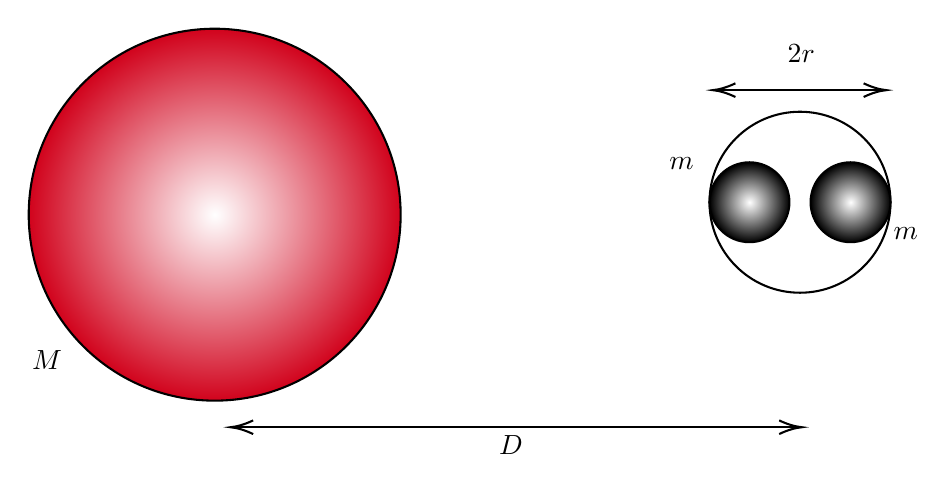
\begin{tikzpicture}[x=0.75pt,y=0.75pt,yscale=-1,xscale=1]
		%uncomment if require: \path (0,592); %set diagram left start at 0, and has height of 592
		
		% Gradient Info
  
		\tikzset {_6f5u4bw5z/.code = {\pgfsetadditionalshadetransform{ \pgftransformshift{\pgfpoint{0 bp } { 0 bp }  }  \pgftransformscale{1 }  }}}
		\pgfdeclareradialshading{_sdq9rs96l}{\pgfpoint{0bp}{0bp}}{rgb(0bp)=(1,1,1);
		rgb(0bp)=(1,1,1);
		rgb(25bp)=(0.82,0.01,0.11);
		rgb(400bp)=(0.82,0.01,0.11)}
		
		% Gradient Info
		  
		\tikzset {_uhtjc8br8/.code = {\pgfsetadditionalshadetransform{ \pgftransformshift{\pgfpoint{0 bp } { 0 bp }  }  \pgftransformscale{1 }  }}}
		\pgfdeclareradialshading{_r2zoicgth}{\pgfpoint{0bp}{0bp}}{rgb(0bp)=(1,1,1);
		rgb(0bp)=(1,1,1);
		rgb(25bp)=(0,0,0);
		rgb(400bp)=(0,0,0)}
		
		% Gradient Info
		  
		\tikzset {_ttpdul3zw/.code = {\pgfsetadditionalshadetransform{ \pgftransformshift{\pgfpoint{0 bp } { 0 bp }  }  \pgftransformscale{1 }  }}}
		\pgfdeclareradialshading{_73j08gyyo}{\pgfpoint{0bp}{0bp}}{rgb(0bp)=(1,1,1);
		rgb(0bp)=(1,1,1);
		rgb(25bp)=(0,0,0);
		rgb(400bp)=(0,0,0)}
		
		%Shape: Circle [id:dp6935061972601739] 
		\path  [shading=_sdq9rs96l,_6f5u4bw5z] (100.8,153.6) .. controls (100.8,104.12) and (140.92,64) .. (190.4,64) .. controls (239.88,64) and (280,104.12) .. (280,153.6) .. controls (280,203.08) and (239.88,243.2) .. (190.4,243.2) .. controls (140.92,243.2) and (100.8,203.08) .. (100.8,153.6) -- cycle ; % for fading 
		 \draw   (100.8,153.6) .. controls (100.8,104.12) and (140.92,64) .. (190.4,64) .. controls (239.88,64) and (280,104.12) .. (280,153.6) .. controls (280,203.08) and (239.88,243.2) .. (190.4,243.2) .. controls (140.92,243.2) and (100.8,203.08) .. (100.8,153.6) -- cycle ; % for border 
		
		%Straight Lines [id:da7280068796924615] 
		\draw    (200,256) -- (471.3,256) ;
		\draw [shift={(473.3,256)}, rotate = 180] [color={rgb, 255:red, 0; green, 0; blue, 0 }  ][line width=0.75]    (10.93,-3.29) .. controls (6.95,-1.4) and (3.31,-0.3) .. (0,0) .. controls (3.31,0.3) and (6.95,1.4) .. (10.93,3.29)   ;
		\draw [shift={(198,256)}, rotate = 0] [color={rgb, 255:red, 0; green, 0; blue, 0 }  ][line width=0.75]    (10.93,-3.29) .. controls (6.95,-1.4) and (3.31,-0.3) .. (0,0) .. controls (3.31,0.3) and (6.95,1.4) .. (10.93,3.29)   ;
		%Shape: Circle [id:dp6956624054740008] 
		\draw   (428.8,147.6) .. controls (428.8,123.52) and (448.32,104) .. (472.4,104) .. controls (496.48,104) and (516,123.52) .. (516,147.6) .. controls (516,171.68) and (496.48,191.2) .. (472.4,191.2) .. controls (448.32,191.2) and (428.8,171.68) .. (428.8,147.6) -- cycle ;
		%Shape: Circle [id:dp3613558976265463] 
		\path  [shading=_r2zoicgth,_uhtjc8br8] (428.8,147.6) .. controls (428.8,136.97) and (437.42,128.35) .. (448.05,128.35) .. controls (458.68,128.35) and (467.3,136.97) .. (467.3,147.6) .. controls (467.3,158.23) and (458.68,166.85) .. (448.05,166.85) .. controls (437.42,166.85) and (428.8,158.23) .. (428.8,147.6) -- cycle ; % for fading 
		 \draw   (428.8,147.6) .. controls (428.8,136.97) and (437.42,128.35) .. (448.05,128.35) .. controls (458.68,128.35) and (467.3,136.97) .. (467.3,147.6) .. controls (467.3,158.23) and (458.68,166.85) .. (448.05,166.85) .. controls (437.42,166.85) and (428.8,158.23) .. (428.8,147.6) -- cycle ; % for border 
		
		%Shape: Circle [id:dp6759589316428882] 
		\path  [shading=_73j08gyyo,_ttpdul3zw] (477.5,147.6) .. controls (477.5,136.97) and (486.12,128.35) .. (496.75,128.35) .. controls (507.38,128.35) and (516,136.97) .. (516,147.6) .. controls (516,158.23) and (507.38,166.85) .. (496.75,166.85) .. controls (486.12,166.85) and (477.5,158.23) .. (477.5,147.6) -- cycle ; % for fading 
		 \draw   (477.5,147.6) .. controls (477.5,136.97) and (486.12,128.35) .. (496.75,128.35) .. controls (507.38,128.35) and (516,136.97) .. (516,147.6) .. controls (516,158.23) and (507.38,166.85) .. (496.75,166.85) .. controls (486.12,166.85) and (477.5,158.23) .. (477.5,147.6) -- cycle ; % for border 
		
		%Straight Lines [id:da2765229200603432] 
		\draw    (432.35,93.6) -- (512,93.6) ;
		\draw [shift={(514,93.6)}, rotate = 180] [color={rgb, 255:red, 0; green, 0; blue, 0 }  ][line width=0.75]    (10.93,-3.29) .. controls (6.95,-1.4) and (3.31,-0.3) .. (0,0) .. controls (3.31,0.3) and (6.95,1.4) .. (10.93,3.29)   ;
		\draw [shift={(430.35,93.6)}, rotate = 0] [color={rgb, 255:red, 0; green, 0; blue, 0 }  ][line width=0.75]    (10.93,-3.29) .. controls (6.95,-1.4) and (3.31,-0.3) .. (0,0) .. controls (3.31,0.3) and (6.95,1.4) .. (10.93,3.29)   ;
		
		% Text Node
		\draw (101,217.4) node [anchor=north west][inner sep=0.75pt]    {$M$};
		% Text Node
		\draw (326,258.4) node [anchor=north west][inner sep=0.75pt]    {$D$};
		% Text Node
		\draw (408,124.4) node [anchor=north west][inner sep=0.75pt]    {$m$};
		% Text Node
		\draw (516,158.4) node [anchor=north west][inner sep=0.75pt]    {$m$};
		% Text Node
		\draw (465,70.4) node [anchor=north west][inner sep=0.75pt]    {$2r$};
		\end{tikzpicture}
		\vspace*{3mm}
		\caption{Configuration for the study of the Roche limit}
	\end{figure}
	The planet is a sphere of radius $R$, mass $M$,  volume density $\rho_P$, located at a distance $D$ of the satellite axis.
	
	The planet exerts on the satellite the gravitational attraction:
	
	The difference of forces between the two masses is:
	
	We can consider that $r \ll D$, giving:
	
	So the difference in force is
	
	If the satellite cohesive force result in the gravitational attraction between the two masses:
	
	The satellite is destroyed if the difference in strength between the two masses is greater than the cohesive force:
	
	But we have the relations:
	
	Therefore we get:
	
	and we deduce of it the "\NewTerm{Roche limit}\index{Roche limit}":
	
	Depending on the approach and the approximations there can be a factor $3$ between some results.
	\begin{tcolorbox}[title=Remark,arc=10pt,breakable,drop lifted shadow,
  skin=enhanced,
  skin first is subskin of={enhancedfirst}{arc=10pt,no shadow},
  skin middle is subskin of={enhancedmiddle}{arc=10pt,no shadow},
  skin last is subskin of={enhancedlast}{drop lifted shadow}]
	For example the calculations given on Wikipedia consider only the difference in the primary's gravitational pull on the center of the satellite and on the edge of the satellite closest to the primary. This means that the main mass only apply one force momentum. But in fact this is not accurate as what interest us is the difference between the two extremities. This is why there is a factor $2$ between the Wikipedia calculations and ours (with our result the satellite will break twice the distance of that given by Wikipedia).
	\end{tcolorbox}
	
	Since in this calculation, we considered a satellite as a two point masses without rotation, and again we have assumed that the satellite's cohesion was provided exclusively by gravitational interactions, this value is just an order of magnitude for rigid body where material is only aggregated by gravity (and not molecular forces).
	
	The Roche limit is one (but not the only one!) source of rings around planets as depicted by the illustration below:
	\begin{figure}[H]
		\centering
		\includegraphics[scale=0.8]{img/cosmology/roche_limit_ring_formation.jpg}
		\caption[]{Roche limit as one of the sources of planetary rings}
	\end{figure}
	
	\pagebreak
	\subsection{Keplerian Orbitals}\label{keplerian orbitals}
	Observation (main tool of the physicist and engineer for recall...) suggests at first glance, that the trajectories of celestial bodies in orbit around stars are indeed conical type (whew!) in the heliocentric reference frame. Knowing this, we can, in order to facilitate the calculation, anticipate the complexity of calculations and express the dynamics directly from a material point in polar coordinates.

	As we saw it in the section Vector Calculus (see page \pageref{polar coordinates}), the speed in polar coordinate is expressed by the relation (we changed the angle Greek letter notation to adapt it to the tradition in astronomy):
	
	where to recall the first term is the radial velocity component and the second component the tangential (angular) velocity!

	For acceleration (the proof is also in the section of Vector Calculus at the same page):
	
	Now that we have the tools, let us get to the case of Keplerian orbits in the case of a static Newtonian field.

	There are to our knowledge two main ways of doing the necessary mathematical developments but that do not give (to our knowledge) the same level of detailed results. The first approach provides finer results but is sometimes a bit do-it-yourself sometimes... is based on the use of the radial velocity and an important relation in astronomy, named the "first Binet formula". The second approach is simpler and more elegant, it uses the radial acceleration to approach the problem and we get a special relation named the "second Binet formula".
	
	\subsubsection{First Binet Formula (radial velocity)}\label{first Binet formula}
	To start with this first approach to the problem, remember that we have already proved earlier that:
	
	However, it is unlikely that the main body is a perfect and homogeneous sphere ... so Astrophysicists have the habit of noting Newtonian potential $U$ under the form:
	
	where $\mu=GM$ is named "\NewTerm{gravitational constant of the star}\index{gravitational constant of a star}" (even if it is not always a star...) and where $f$ is a function representing the heterogeneity of the star.
	
	If there is one place in the universe where the laws of mechanics are perfectly verifiable, it is space, because the friction or causes of dissipation are extremely small. Within the field of a single force deriving from a potential, the movement satisfies the conservation of mechanical energy.

	Thus we end in the so-named "\NewTerm{energy equation}\index{energy equation}", wherein $E$ denotes the "\NewTerm{specific energy}\index{specific energy}" per unit weight (kilogram):
	
	Therefore:
	
	The Newtonian gravitational force is central, thus having a null torque force at the center O of the main body. This results in the conservation of angular momentum in norm and direction, either:
	
	The vector $\vec{W}$ is the normalized vector of $\vec{b}$ or of $\vec{h}$ named the "\NewTerm{reduced momentum}\index{reduced momentum}". $K$ is the constant of areas (\SeeChapter{see page \pageref{constant areal velocity}}) such that:
	
	We recall to the reader that the norm of the speed expressed in polar coordinates is given by the relation (remember that the both vectors of the polar base are orthogonal and that we can therefore apply the Pythagorean theorem to calculate the norm as it has been proved in the section of Vector Calculus):
	
	Which gives us the possibility to write the area constant $K$ as:
	
	Let us now put ourselves in the orbital plane, in polar coordinates.
	
	Given the relation already proved and known:
	
	and its squared norm:
	
	Or in the case of a central force (conservation of angular momentum):
	
	Let's put this in the prior-previous expression of $v^2$, then we have:
	Let us put this in the expression prior-previous expression of $v^2$, then we have:
	
	The relation:
	
	is named "\NewTerm{Binet's first formula}\index{Binet's first formula}".
	
	By equating with the expression of $v^2$ resulting from the conservation of energy that we get earlier above, we have:
	
	This gives us a rather complicated differential equation:
	
	And then we wonder how we can get out of such a situation? After some hours of reflection ... we realize that takes to make a substitution. After another hour of neural chaos this ultimately leads to an end.... We decide to put (we have the right to do it!), knowing that $r$ is a function of $u$ and $\theta$:
	
	Let us derivate merrily relatively to $\theta$:
	
	Substituting in the differential equation:
	
	After simplification we get:
	
	We separate the variables to integrate:
	
	We have two solutions according to the sign we choose. However, at the end of the resolution, we notice that the only physically interesting choice is the negative sign. We have proved in the section of Differential and Integral Calculus during our study of common derivatives (see page \pageref{usual derivatives}) that:
	
	We will chose the primitive in cosine and therefore we have:
	
	We leave, by approximation, the constant of integration that would involve very small oscillations in the orbit's path (if you do a study or a homework on this topic, you can transfer me your plots with or without the constant, it would interest me as I don't  have time to do it myself).

	This allows us to get:
	
	Now we see that our choice of the sign for the integration is fully justified because now, if we do a little recall on conics (\SeeChapter{see section Analytical Geometry page \pageref{conics}}), we see that after rearrangement:
	
	So finally we have a relation of the following form if we choose $\theta_0=0$:
	
	where by analogy with the section of Analytical Geometry $e$ is the eccentricity (let us recall that $e=c/a<1$ with $a$ the semi big axes and $c$ the distance to the center of the ellipse to the focal) and $p$ the focal parameter ($p=b^2/a$) of an ellipse. This corresponds well to the trajectories that follow celestial bodies in orbit.
	
	We thus fall back on our the first  Kepler "law"... so as we can see it, it can be proven!

	In our case, we have after simplification to resume:
	
	where (for recall) $K$ is the areas constant :
	
	and $\mu$ is the gravitation constant of the celestial body:
	
	and finally $E$ the specific energy:
	
	The reader could be able to check himself as we have seen in the section of Analytical Geometry in our study conical that if:
	\begin{itemize}
		\item If $E=0$ such that $e=1$ we have an opened orbit in the form of a parabola

		\item If $E>0$ such that $e>1$ we have an opened orbit in the form of an hyperbola

		\item If $E\leq 0$ such that $0\geq e <1$ we have a closed orbit in the form of an ellipse or a circle
	\end{itemize}
	\begin{figure}[H]
		\centering
		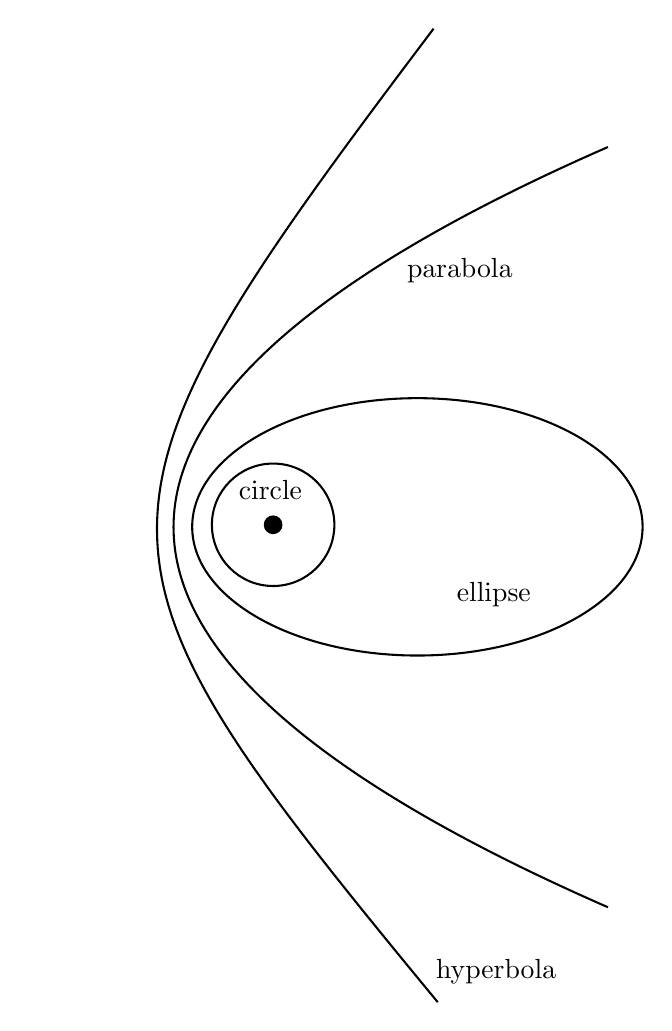
\begin{tikzpicture}[x=0.75pt,y=0.75pt,yscale=-1,xscale=1]
		%uncomment if require: \path (0,638); %set diagram left start at 0, and has height of 638
		
		%Shape: Circle [id:dp8086840374328494] 
		\draw  [fill={rgb, 255:red, 0; green, 0; blue, 0 }  ,fill opacity=1 ] (266,248) .. controls (266,245.79) and (267.79,244) .. (270,244) .. controls (272.21,244) and (274,245.79) .. (274,248) .. controls (274,250.21) and (272.21,252) .. (270,252) .. controls (267.79,252) and (266,250.21) .. (266,248) -- cycle ;
		%Shape: Circle [id:dp35477612057831287] 
		\draw   (240.5,248) .. controls (240.5,231.71) and (253.71,218.5) .. (270,218.5) .. controls (286.29,218.5) and (299.5,231.71) .. (299.5,248) .. controls (299.5,264.29) and (286.29,277.5) .. (270,277.5) .. controls (253.71,277.5) and (240.5,264.29) .. (240.5,248) -- cycle ;
		%Shape: Ellipse [id:dp2228918824859636] 
		\draw   (231,249) .. controls (231,214.76) and (279.58,187) .. (339.5,187) .. controls (399.42,187) and (448,214.76) .. (448,249) .. controls (448,283.24) and (399.42,311) .. (339.5,311) .. controls (279.58,311) and (231,283.24) .. (231,249) -- cycle ;
		%Shape: Parabola [id:dp6127285431813179] 
		\draw   (431.3,66) .. controls (152.24,188.09) and (152.24,310.19) .. (431.3,432.27) ;
		%Curve Lines [id:da4892890038952771] 
		\draw    (347.3,9) .. controls (168.3,246) and (170.3,261) .. (349.3,478) ;
		
		% Text Node
		\draw (252,225) node [anchor=north west][inner sep=0.75pt]   [align=left] {circle};
		% Text Node
		\draw (357,274) node [anchor=north west][inner sep=0.75pt]   [align=left] {ellipse};
		% Text Node
		\draw (333,118) node [anchor=north west][inner sep=0.75pt]   [align=left] {parabola};
		% Text Node
		\draw (347,456) node [anchor=north west][inner sep=0.75pt]   [align=left] {hyperbola};
		\end{tikzpicture}
		\vspace*{3mm}
		\caption[]{Reminders of conical but "orbit" oriented}
	\end{figure}
	Finally, if we inject:
	
	in the first Binet formula:
	
	then we get the velocity in any point of the ellipse based on the primary variable parameter which is therefore the angle:
	
	Hence:
	
	There is another famous and simple relation of the radial velocity named the vis-viva equation that we will in the section of Aerospace Engineering at page \pageref{vis-viva equation}:
	
	
	\subsubsection{Second Binet Formula (radial acceleration)}
	Let us now see the approach based on the radial acceleration which, while being more elegant, allows us to get a result less fine-tuned on the ellipse parameters.

	So we start from the expression of the acceleration in polar coordinates (\SeeChapter{see section Vector Calculus page \pageref{polar coordinates}}):
	
	We can simplify the writing of the second term:
	
	Now we have seen just above that:
	
	and so:
	
	Then the acceleration is reduced to:
	
	We can eliminate the time by writing:
	
	and:
	
	Then we get:
	
	And so it comes to the standard "\NewTerm{Binet's second formula}\index{Binet's second formula}":
	
	But according to Newton's second law and his law of gravitation, we have:
		
	We then get another form of the Binet's second formula:
	
	Or after simplification and choosing the sign of the acceleration at our convenience to get rid of the "-" sign, we have:
	
	By isolating the constants, we get:
	
	After a change of variables we recognize the particular case of a differential equation of the second order we have already met several times so far in various sections of this book and that will meet again:
	
	As it is customary, however, we will show the details of the resolution. The equation without second member is (\SeeChapter{see section Differential and Integral Calculus page \pageref{second order differential equations}}):
	
	We then have the discriminant that is negative since:
	
	We then saw in the section of Differential and Integral Calculus (see page \pageref{second order differential equations}), that in this situation the solution of the homogeneous equation was of the form:
	
	Thus in the situation we are concerned, we have:
	
	We inject the solution into the homogeneous differential equation with second member:
	
	and we see immediately that for the equality to be satisfied, the general solution is:
	
	Or after rearrangement:
	
	And choosing the initial angle as zero, so we find well:
	
	at the difference with the first method of resolution that the value of the constant $A$ is unknown.
	
	Let us now come back on:
	
	By expliciting:
	
	And as (\SeeChapter{see section Classical Mechanics page \pageref{kinematics of circular motion}}):
	
	So if we choose a particular point of reference of the path (not necessarily circular path), we have:
	
	Then we have:
	
	If we put the phase shift as zero relatively to the reference chosen radius earlier above, the expression simplifies to:
	
	To determine the constant $A$, we place ourselves in the case where $\theta=0$ and imposes that the radius $r$ is the initial radius measured when this angle is zero. Then we have:
	
	This implies immediately:
	
	Thus after elementary rearrangements and simplifications:
	
	And therefore we have a direct correspondence:
	
	And as the eccentricity $e$ is known for a circular, parabolic, elliptical or another trajectory of the conical type... it gets us very easy to deduce the velocity at the particular point of the initial radius $r$ of the studied object.

	The closest distance of the object orbiting around its central star (focus), will be given by the value that can takes $r$ in the relation:
	
	if we impose $\theta=0$.

	In the case of an elliptical orbit it is the "\NewTerm{perigee}\index{perigee}" to be assimilated to the initial radius as the point where the measurement of the radial velocity was the most accurate.

	The farthest distance from the focus will be given by putting the angle as being $180^\circ$ ($\pi$) and then we name it "\NewTerm{apogee}\index{apogee}".
	
	\pagebreak
	\subsubsection{Keplerian orbital period}
	The Kepler's law of equal areas allows, as we already know, to calculate the Keplerian orbital period $T$. In fact, the area $S$ of the ellipse being equal to $S=\pi a b$ (\SeeChapter{see section Geometric Shapes page \pageref{ellipse}}) and having already determined during our definition of the angular momentum that (\SeeChapter{see section Classical Mechanics page \pageref{angular momentum}}):
	 
	It comes naturally:
	
	Moreover, the study of conics (\SeeChapter{see section Analytical Geometry page \pageref{parameter of the ellipse}}) has showed us that:
	
	and we have defined above:
	
	So we have the relation:
	
	and then we fall back again on the third Kepler's law:
	
	which validates our previous calculations.
	
	Obviously the latter relation is only available for $T$ where the corresponding speed is non relativistic otherwise we have to use General Relativity tools.
	
	Before we continue... here are some useful data for this section and for that for Aerospace Engineering (i.e. "space dynamics") relatively to our knowledge in the state of year 12018 according to holocene calendar (various sources were used for these tables but the main one is Wikipedia):
	\begin{table}[H]
		\centering
		\begin{tabular}{|l|c|}
		\hline
		\multicolumn{2}{|c|}{\cellcolor[gray]{0.75}\textbf{Mercury (terrestrial) $\mercury$}} \\ \hline
		Mass & $3.3011\cdot 10^{23}$ {[}kg{]} \\ \hline
		Mean density & $5.427\;[\text{g}\cdot \text{cm}^{-3}]$ \\ \hline
		Mean radius & $2,439.7$ {[}km{]} \\ \hline
		Equatorial radius & $2,439.7$  {[}km{]} \\ \hline
		Polar radius & $2,439.7$ {[}km{]} \\ \hline
		Circumference & $15,239.08$ {[}km{]} \\ \hline
		Surface gravity & $3.7 \; [\text{m}\cdot \text{s}^{-2}]$ \\ \hline
		Escape velocity & $4.25\;[\text{km}\cdot\text{s}^{-1}]$ \\ \hline
		Sidereal rotation period & 58.646 d \\ \hline
		Equatorial rotation velocity & $10.892\;[\text{km}\cdot\text{h}^{-1}]$ \\ \hline
		Axial tilt & $0.034^\circ$ \\ \hline
		Ecliptic inclination & $7.00^\circ$ \\ \hline
		Surface pressure & $0$ {[}hPa{]} (at MSL) \\ \hline
		Aphelion & $69,816,900$ {[}km{]} \\ \hline
		Perihelion & $46,001,200$ {[}km{]} \\ \hline
		Semi-major axis & $57,909,050$ {[}km{]} \\ \hline
		Eccentricity & $0.205630$ \\ \hline
		Orbital period & $87.969 $ {[}d{]} \\ \hline
		Average orbital speed & $47.362\;[\text{km}\cdot\text{s}^{-1}]$ \\ \hline
		Average Temperature & $363$ {[}K{]} \\ \hline
		Number of satellites & $0$ \\ \hline
		\end{tabular}
		\caption{Some Mercury characteristics}
	\end{table}
	
	\begin{table}[H]
		\centering
		\begin{tabular}{|l|c|}
		\hline
		\multicolumn{2}{|c|}{\cellcolor[gray]{0.75}\textbf{Venus (terrestrial) $\venus$}} \\ \hline
		Mass & $4.8675\cdot 10^{24}$ {[}kg{]} \\ \hline		
		Mean density & $5.243\;[\text{g}\cdot \text{cm}^{-3}]$ \\ \hline
		Mean radius & $6,051.8$ {[}km{]} \\ \hline
		Equatorial radius & $6,051.8$  {[}km{]} \\ \hline
		Polar radius & $6,051.8$ {[}km{]} \\ \hline
		Circumference & $38,019.55$ {[}km{]} \\ \hline
		Surface gravity & $8.87 \; [\text{m}\cdot \text{s}^{-2}]$ \\ \hline
		Escape velocity & $10.36 \;[\text{km}\cdot\text{s}^{-1}]$ \\ \hline
		Sidereal rotation period & -243.025 d (retrograde) \\ \hline
		Equatorial rotation velocity & $6.52\;[\text{km}\cdot\text{h}^{-1}]$ \\ \hline
		Axial tilt & $2.64^\circ$ \\ \hline
		Ecliptic inclination & $3.39^\circ$ \\ \hline
		Surface pressure & $90,000$ {[}hPa{]} (at MSL) \\ \hline
		Aphelion & $108,939,000$ {[}km{]} \\ \hline
		Perihelion & $107,477,000$ {[}km{]} \\ \hline
		Semi-major axis & $108,208,000$ {[}km{]} \\ \hline
		Eccentricity & $0.006772$ \\ \hline
		Orbital period & $224.701$ {[}d{]} \\ \hline
		Average orbital speed & $35.02\;[\text{km}\cdot\text{s}^{-1}]$ \\ \hline
		Average Temperature & $737$ {[}K{]} \\ \hline
		Number of satellites & $0$ \\ \hline
		\end{tabular}
		\caption{Some Venus characteristics}
	\end{table}
	
	\begin{table}[H]
		\centering
		\begin{tabular}{|l|c|}
		\hline
		\multicolumn{2}{|c|}{\cellcolor[gray]{0.75}\textbf{Earth (terrestrial) $\earth$}} \\ \hline
		Mass & $5.97237\cdot 10^{24}$ {[}kg{]} \\ \hline	
		Mean density & $5.514\;[\text{g}\cdot \text{cm}^{-3}]$ \\ \hline
		Mean radius & $6,371.0$ {[}km{]} \\ \hline
		Equatorial radius & $6,378.1$  {[}km{]} \\ \hline
		Polar radius & $6,356.8$ {[}km{]} \\ \hline
		Circumference & $40,075.017$ {[}km{]} \\ \hline
		Surface gravity & $9.807\; [\text{m}\cdot \text{s}^{-2}]$ \\ \hline
		Escape velocity & $11.186\;[\text{km}\cdot\text{s}^{-1}]$ \\ \hline
		Sidereal rotation period & 23h 56m 4.100s \\ \hline
		Equatorial rotation velocity & $0.465\;[\text{km}\cdot\text{s}^{-1}]$ \\ \hline
		Axial tilt & $23.439281^\circ$ \\ \hline
		Ecliptic inclination & $0.00005^\circ$ \\ \hline
		Surface pressure & $101.325$ {[}hPa{]} (at MSL) \\ \hline
		Aphelion & $152,100,000$ {[}km{]} \\ \hline
		Perihelion & $147,095,000$ {[}km{]} \\ \hline
		Semi-major axis & $149,598,023$ {[}km{]} \\ \hline
		Eccentricity & $0.0167086$ \\ \hline
		Orbital period & $365.256363004$ {[}d{]} \\ \hline
		Average orbital speed & $29.78\;[\text{km}\cdot\text{s}^{-1}]$ \\ \hline
		Average Temperature & $287$ {[}K{]} \\ \hline
		Number of satellites & $1$ \\ \hline
		\end{tabular}
		\caption{Some Earth characteristics}
	\end{table}
	
	\begin{table}[H]
		\centering
		\begin{tabular}{|l|c|}
		\hline
		\multicolumn{2}{|c|}{\cellcolor[gray]{0.75}\textbf{Mars (terrestrial) $\mars$}} \\ \hline
		Mass & $6.4171\cdot 10^{23}$ {[}kg{]} \\ \hline		
		Mean density & $3.9335\;[\text{g}\cdot \text{cm}^{-3}]$ \\ \hline
		Mean radius & $3,389.5$ {[}km{]} \\ \hline
		Equatorial radius & $3,396.2$ {[}km{]} \\ \hline
		Polar radius & $3376.2$ {[}km{]} \\ \hline
		Circumference & $21296.856$ {[}km{]} \\ \hline
		Surface gravity & $3.711\; [\text{m}\cdot \text{s}^{-2}]$ \\ \hline
		Escape velocity & $5.027 \;[\text{km}\cdot\text{s}^{-1}]$ \\ \hline
		Sidereal rotation period & 24h 37m 22s \\ \hline
		Equatorial rotation velocity & $0.241\;[\text{km}\cdot\text{s}^{-1}]$ \\ \hline
		Axial tilt & $25.19^\circ$ \\ \hline
		Ecliptic inclination & $1.85^\circ$ \\ \hline
		Surface pressure & $2-10$ {[}hPa{]} (at MSL) \\ \hline
		Aphelion & $249,200,000$ {[}km{]} \\ \hline
		Perihelion & $206,700,000$ {[}km{]} \\ \hline
		Semi-major axis & $227,939,200$ {[}km{]} \\ \hline
		Eccentricity & $0.0934$ \\ \hline
		Orbital period & $686.971$ {[}d{]} \\ \hline
		Average orbital speed & $24.007\;[\text{km}\cdot\text{s}^{-1}]$ \\ \hline
		Average Temperature & $213$ {[}K{]} \\ \hline
		Number of satellites & $2$ \\ \hline
		\end{tabular}
		\caption{Some Mars characteristics}
	\end{table}
	
	\begin{table}[H]
		\centering
		\begin{tabular}{|l|c|}
		\hline
		\multicolumn{2}{|c|}{\cellcolor[gray]{0.75}\textbf{Jupiter (gaseous) $\jupiter$}} \\ \hline
		Mass & $1.8982\cdot 10^{27}$ {[}kg{]} \\ \hline
		Mean density & $1.326\;[\text{g}\cdot \text{cm}^{-3}]$ \\ \hline
		Mean radius & $69,911$ {[}km{]} \\ \hline
		Equatorial radius & $71,492$  {[}km{]} \\ \hline
		Polar radius & $66,854$ {[}km{]} \\ \hline
		Circumference & $439,263.76$ {[}km{]} \\ \hline
		Surface gravity & $24.79\; [\text{m}\cdot \text{s}^{-2}]$ \\ \hline
		Escape velocity & $59.5 \;[\text{km}\cdot\text{s}^{-1}]$ \\ \hline
		Sidereal rotation period & 9h 55m 30s \\ \hline
		Equatorial rotation velocity & $12.6\;[\text{km}\cdot\text{s}^{-1}]$ \\ \hline
		Axial tilt & $3.13^\circ$ \\ \hline
		Ecliptic inclination & $1.303^\circ$ \\ \hline
		Surface pressure & $-$ {[}hPa{]} (at MSL) \\ \hline
		Aphelion & $816,620,000$ {[}km{]} \\ \hline
		Perihelion & $740,520,000$ {[}km{]} \\ \hline
		Semi-major axis & $778,570,000$ {[}km{]} \\ \hline
		Eccentricity & $0.0489$ \\ \hline
		Orbital period & $4,332.59$ {[}d{]} \\ \hline
		Average orbital speed & $13.07\;[\text{km}\cdot\text{s}^{-1}]$ \\ \hline
		Average Temperature & $165$ {[}K{]} \\ \hline
		Number of satellites & $69$ \\ \hline
		\end{tabular}
		\caption{Some Jupiter characteristics}
	\end{table}
	
	\begin{table}[H]
		\centering
		\begin{tabular}{|l|c|}
		\hline
		\multicolumn{2}{|c|}{\cellcolor[gray]{0.75}\textbf{Saturn (gaseous) $\saturn$}} \\ \hline
		Mass & $5.6834\cdot 10^{26}$ {[}kg{]} \\ \hline
		Mean density & $0.687\;[\text{g}\cdot \text{cm}^{-3}]$ \\ \hline
		Mean radius & $58,232$ {[}km{]} \\ \hline
		Equatorial radius & $60,268$ {[}km{]} \\ \hline
		Polar radius & $54,364$ {[}km{]} \\ \hline
		Circumference & $365,882.44$ {[}km{]} \\ \hline
		Surface gravity & $10.44\; [\text{m}\cdot \text{s}^{-2}]$ \\ \hline
		Escape velocity & $35.5 \;[\text{km}\cdot\text{s}^{-1}]$ \\ \hline
		Sidereal rotation period & 10h 33m \\ \hline
		Equatorial rotation velocity & $9.87\;[\text{km}\cdot\text{s}^{-1}]$ \\ \hline
		Axial tilt & $26.73^\circ$ \\ \hline
		Ecliptic inclination & $2.485^\circ$ \\ \hline
		Surface pressure & $-$ {[}hPa{]} (at MSL) \\ \hline
		Aphelion & $1,514,000,000$ {[}km{]} \\ \hline
		Perihelion & $1,352,550,000$ {[}km{]} \\ \hline
		Semi-major axis & $1,433,530,000$ {[}km{]} \\ \hline
		Eccentricity & $0.0565$ \\ \hline
		Orbital period & $10,759.22 $ {[}d{]} \\ \hline
		Average orbital speed & $9.68\;[\text{km}\cdot\text{s}^{-1}]$ \\ \hline
		Average Temperature & $100-160$ {[}K{]} \\ \hline
		Number of satellites & $62$ \\ \hline
		\end{tabular}
		\caption{Some Saturn characteristics}
	\end{table}
	
	\begin{table}[H]
		\centering
		\begin{tabular}{|l|c|}
		\hline
		\multicolumn{2}{|c|}{\cellcolor[gray]{0.75}\textbf{Uranus (gaseous) $\uranus$}} \\ \hline
		Mass & $8.6810\cdot 10^{25}$ {[}kg{]} \\ \hline	
		Mean density & $1.27\;[\text{g}\cdot \text{cm}^{-3}]$ \\ \hline
		Mean radius & $25,362$ {[}km{]} \\ \hline
		Equatorial radius & $25,559 $ {[}km{]} \\ \hline
		Polar radius & $24,973$ {[}km{]} \\ \hline
		Circumference & $159,354.14$ {[}km{]} \\ \hline
		Surface gravity & $8.69\; [\text{m}\cdot \text{s}^{-2}]$ \\ \hline
		Escape velocity & $21.3\;[\text{km}\cdot\text{s}^{-1}]$ \\ \hline
		Sidereal rotation period & -17h 14m 24s (retrograde) \\ \hline
		Equatorial rotation velocity & $2.59\;[\text{km}\cdot\text{s}^{-1}]$ \\ \hline
		Axial tilt & $97.77^\circ$ \\ \hline
		Ecliptic inclination & $0.773^\circ$ \\ \hline
		Surface pressure & $-$ {[}hPa{]} (at MSL) \\ \hline
		Aphelion & $3,008,000,000$ {[}km{]} \\ \hline
		Perihelion & $2,742,000,000$ {[}km{]} \\ \hline
		Semi-major axis & $2,875,000,000$ {[}km{]} \\ \hline
		Eccentricity & $0.046$ \\ \hline
		Orbital period & $30,688.5$ {[}d{]} \\ \hline
		Average orbital speed & $6.80\;[\text{km}\cdot\text{s}^{-1}]$ \\ \hline
		Average Temperature & $76$ {[}K{]} \\ \hline
		Number of satellites & $27$ \\ \hline
		\end{tabular}
		\caption{Some Uranus characteristics}
	\end{table}
	
	\begin{table}[H]
		\centering
		\begin{tabular}{|l|c|}
		\hline
		\multicolumn{2}{|c|}{\cellcolor[gray]{0.75}\textbf{Neptune (gaseous) $\neptune$}} \\ \hline
		Mass & $1.0243\cdot 10^{26}$ {[}kg{]} \\ \hline
		Mean density & $1.638\;[\text{g}\cdot \text{cm}^{-3}]$ \\ \hline
		Mean radius & $24,622$ {[}km{]} \\ \hline
		Equatorial radius & $24,764$ {[}km{]} \\ \hline
		Polar radius & $24,341$ {[}km{]} \\ \hline
		Circumference & $154,704.58$ {[}km{]} \\ \hline
		Surface gravity & $11.15\; [\text{m}\cdot \text{s}^{-2}]$ \\ \hline
		Escape velocity & $23.5\;[\text{km}\cdot\text{s}^{-1}]$ \\ \hline
		Sidereal rotation period & 16h 6m 36s \\ \hline
		Equatorial rotation velocity & $2.68\;[\text{km}\cdot\text{s}^{-1}]$ \\ \hline
		Axial tilt & $28.32^\circ$ \\ \hline
		Ecliptic inclination & $1.767^\circ$ \\ \hline
		Surface pressure & $-$ {[}hPa{]} (at MSL) \\ \hline
		Aphelion & $4,540,000,000$ {[}km{]} \\ \hline
		Perihelion & $4,460,000,000$ {[}km{]} \\ \hline
		Semi-major axis & $4,500,000,000$ {[}km{]} \\ \hline
		Eccentricity & $0.009$ \\ \hline
		Orbital period & $60,182$ {[}d{]} \\ \hline
		Average orbital speed & $5.43\;[\text{km}\cdot\text{s}^{-1}]$ \\ \hline
		Average Temperature & $72$ {[}K{]} \\ \hline
		Number of satellites & $14$ \\ \hline
		\end{tabular}
		\caption{Some Neptune characteristics}
	\end{table}
	
	\begin{table}[H]
		\centering
		\begin{tabular}{|l|c|}
		\hline
		\multicolumn{2}{|c|}{\cellcolor[gray]{0.75}\textbf{Pluto (terrestrial dwarf planet) $\pluto$}} \\ \hline
		Mass & $1.303\cdot 10^{22}$ {[}kg{]} \\ \hline
		Mean density & $1.854\;[\text{g}\cdot \text{cm}^{-3}]$ \\ \hline
		Mean radius & $1,188.3$ {[}km{]} \\ \hline
		Equatorial radius & $-$ {[}km{]} \\ \hline
		Polar radius & $-$ {[}km{]} \\ \hline
		Circumference & $7,466.309$ {[}km{]} \\ \hline
		Surface gravity & $0.620\; [\text{m}\cdot \text{s}^{-2}]$ \\ \hline
		Escape velocity & $1.212\;[\text{km}\cdot\text{s}^{-1}]$ \\ \hline
		Sidereal rotation period & 6d 9h 17m 36s \\ \hline
		Equatorial rotation velocity & $0.013\;[\text{km}\cdot\text{s}^{-1}]$ \\ \hline
		Axial tilt & $122.53^\circ$ \\ \hline
		Ecliptic inclination & $17.16^\circ$ \\ \hline
		Surface pressure & $0,01$ {[}hPa{]} (at MSL) \\ \hline
		Aphelion & $7,375,930,000$ {[}km{]} \\ \hline
		Perihelion & $4,436,820,000$ {[}km{]} \\ \hline
		Semi-major axis & $5,906,380,000$ {[}km{]} \\ \hline
		Eccentricity & $0.2488$ \\ \hline
		Orbital period & $90,560$ {[}d{]} \\ \hline
		Average orbital speed & $4.67\;[\text{km}\cdot\text{s}^{-1}]$ \\ \hline
		Average Temperature & $44$ {[}K{]} \\ \hline
		Number of satellites & $5$ \\ \hline
		\end{tabular}
		\caption{Some Pluto characteristics}
	\end{table}
	
	\pagebreak
	\subsubsection{Average distance between two planets}
	Let us consider two planets with the special and ideal case where the orbit are perfectly circular around a given star like below:
	 \begin{figure}[H]
	 	\centering
		% Gradient Info
		  
		\tikzset {_2ojvv7lrk/.code = {\pgfsetadditionalshadetransform{ \pgftransformshift{\pgfpoint{0 bp } { 0 bp }  }  \pgftransformscale{1 }  }}}
		\pgfdeclareradialshading{_nlth2r4ii}{\pgfpoint{0bp}{0bp}}{rgb(0bp)=(0.97,0.91,0.11);
		rgb(0bp)=(0.97,0.91,0.11);
		rgb(25bp)=(0.96,0.65,0.14);
		rgb(400bp)=(0.96,0.65,0.14)}
		\tikzset{every picture/.style={line width=0.75pt}} %set default line width to 0.75pt        
		
		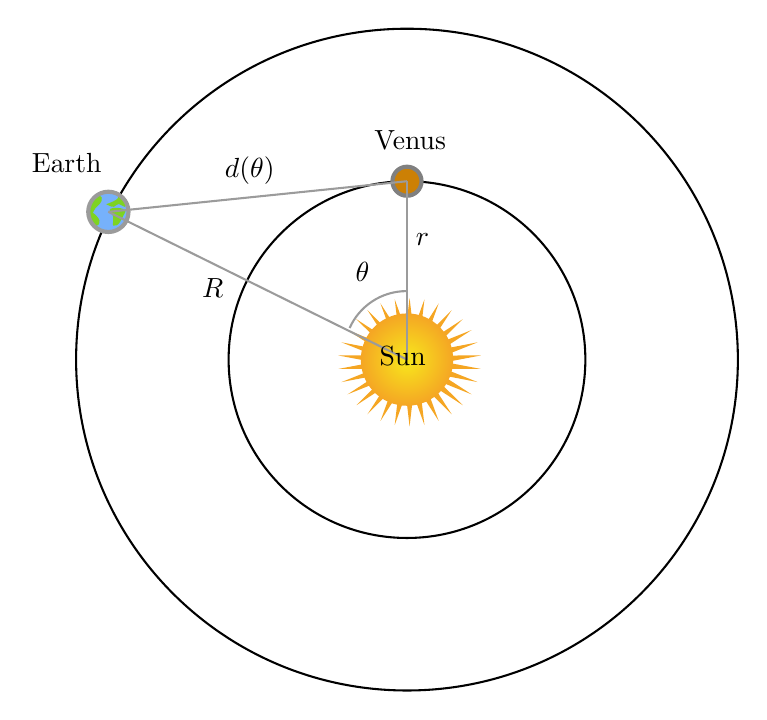
\begin{tikzpicture}[x=0.75pt,y=0.75pt,yscale=-1,xscale=1]
		%uncomment if require: \path (0,1500); %set diagram left start at 0, and has height of 1500
		
		%Shape: Star [id:dp17501130913976493] 
		\draw  [draw opacity=0][fill={rgb, 255:red, 245; green, 166; blue, 35 }  ,fill opacity=1 ] (311.5,236) -- (313.3,251.58) -- (318.67,236.68) -- (316.83,252.26) -- (325.53,238.68) -- (320.13,253.58) -- (331.78,241.92) -- (323.04,255.48) -- (337.14,246.26) -- (325.46,257.89) -- (341.38,251.5) -- (327.26,260.7) -- (344.31,257.42) -- (328.37,263.78) -- (345.81,263.76) -- (328.75,267) -- (345.81,270.24) -- (328.37,270.22) -- (344.31,276.58) -- (327.26,273.3) -- (341.38,282.5) -- (325.46,276.11) -- (337.14,287.74) -- (323.04,278.52) -- (331.78,292.08) -- (320.13,280.42) -- (325.53,295.32) -- (316.83,281.74) -- (318.67,297.32) -- (313.3,282.42) -- (311.5,298) -- (309.7,282.42) -- (304.33,297.32) -- (306.17,281.74) -- (297.47,295.32) -- (302.88,280.42) -- (291.22,292.08) -- (299.96,278.52) -- (285.86,287.74) -- (297.54,276.11) -- (281.62,282.5) -- (295.74,273.3) -- (278.69,276.58) -- (294.63,270.22) -- (277.19,270.24) -- (294.25,267) -- (277.19,263.76) -- (294.63,263.78) -- (278.69,257.42) -- (295.74,260.7) -- (281.62,251.5) -- (297.54,257.89) -- (285.86,246.26) -- (299.96,255.48) -- (291.22,241.92) -- (302.88,253.58) -- (297.47,238.68) -- (306.17,252.26) -- (304.33,236.68) -- (309.7,251.58) -- cycle ;
		%Shape: Circle [id:dp0672915247834267] 
		\draw  [draw opacity=0][shading=_nlth2r4ii,_2ojvv7lrk] (288,265.75) .. controls (288,253.46) and (297.96,243.5) .. (310.25,243.5) .. controls (322.54,243.5) and (332.5,253.46) .. (332.5,265.75) .. controls (332.5,278.04) and (322.54,288) .. (310.25,288) .. controls (297.96,288) and (288,278.04) .. (288,265.75) -- cycle ;
		%Shape: Circle [id:dp3228746468794177] 
		\draw   (224.31,265.75) .. controls (224.31,218.29) and (262.79,179.81) .. (310.25,179.81) .. controls (357.71,179.81) and (396.19,218.29) .. (396.19,265.75) .. controls (396.19,313.21) and (357.71,351.69) .. (310.25,351.69) .. controls (262.79,351.69) and (224.31,313.21) .. (224.31,265.75) -- cycle ;
		%Shape: Circle [id:dp9684857321304758] 
		\draw   (150.83,265.75) .. controls (150.83,177.7) and (222.2,106.33) .. (310.25,106.33) .. controls (398.3,106.33) and (469.67,177.7) .. (469.67,265.75) .. controls (469.67,353.8) and (398.3,425.17) .. (310.25,425.17) .. controls (222.2,425.17) and (150.83,353.8) .. (150.83,265.75) -- cycle ;
		%Shape: Circle [id:dp16846092685147807] 
		\draw  [draw opacity=0][fill={rgb, 255:red, 118; green, 177; blue, 251 }  ,fill opacity=1 ] (156.74,194.57) .. controls (156.74,189.25) and (161.05,184.94) .. (166.37,184.94) .. controls (171.7,184.94) and (176.01,189.25) .. (176.01,194.57) .. controls (176.01,199.9) and (171.7,204.21) .. (166.37,204.21) .. controls (161.05,204.21) and (156.74,199.9) .. (156.74,194.57) -- cycle ;
		%Shape: Polygon Curved [id:ds7972795074912189] 
		\draw  [draw opacity=0][fill={rgb, 255:red, 126; green, 211; blue, 33 }  ,fill opacity=1 ] (167.43,194.56) .. controls (164.76,191.66) and (175.53,192.25) .. (174.6,194.54) .. controls (173.67,196.83) and (173.37,197.3) .. (172.04,199.38) .. controls (170.7,201.46) and (169.59,201.31) .. (168.7,201.17) .. controls (167.8,201.02) and (170.11,197.45) .. (167.43,194.56) -- cycle ;
		%Shape: Polygon Curved [id:ds256038504974734] 
		\draw  [draw opacity=0][fill={rgb, 255:red, 126; green, 211; blue, 33 }  ,fill opacity=1 ] (158.96,188.39) .. controls (161.34,185.42) and (164.05,186.99) .. (163.12,189.28) .. controls (162.2,191.57) and (159.93,192.25) .. (159.26,194.33) .. controls (158.59,196.41) and (157.78,195.97) .. (157.11,195.52) .. controls (156.44,195.08) and (156.59,191.36) .. (158.96,188.39) -- cycle ;
		%Shape: Polygon Curved [id:ds24584635509870933] 
		\draw  [draw opacity=0][fill={rgb, 255:red, 126; green, 211; blue, 33 }  ,fill opacity=1 ] (156.74,195.15) .. controls (156.51,192.4) and (163.01,197.47) .. (162.08,199.75) .. controls (161.16,202.04) and (161.42,199.83) .. (160.97,201.31) .. controls (160.52,202.8) and (159.86,201.76) .. (158.89,200.65) .. controls (157.92,199.53) and (156.96,197.9) .. (156.74,195.15) -- cycle ;
		%Shape: Polygon Curved [id:ds27978768607933] 
		\draw  [draw opacity=0][fill={rgb, 255:red, 126; green, 211; blue, 33 }  ,fill opacity=1 ] (170.92,186.61) .. controls (168.99,184.3) and (176.01,189.22) .. (175.08,191.51) .. controls (174.15,193.8) and (171.59,189.21) .. (170.25,191.29) .. controls (168.92,193.37) and (166.32,191.14) .. (165.43,190.99) .. controls (164.54,190.84) and (172.85,188.91) .. (170.92,186.61) -- cycle ;
		%Shape: Circle [id:dp9218160597156135] 
		\draw  [color={rgb, 255:red, 155; green, 155; blue, 155 }  ,draw opacity=1 ][line width=1.5]  (156.67,194.57) .. controls (156.67,189.22) and (161.02,184.87) .. (166.37,184.87) .. controls (171.73,184.87) and (176.07,189.22) .. (176.07,194.57) .. controls (176.07,199.93) and (171.73,204.27) .. (166.37,204.27) .. controls (161.02,204.27) and (156.67,199.93) .. (156.67,194.57) -- cycle ;
		
		%Shape: Circle [id:dp25942146147006406] 
		\draw  [color={rgb, 255:red, 128; green, 128; blue, 128 }  ,draw opacity=1 ][fill={rgb, 255:red, 204; green, 128; blue, 5 }  ,fill opacity=1 ][line width=1.5]  (303.25,179.81) .. controls (303.25,175.95) and (306.38,172.81) .. (310.25,172.81) .. controls (314.12,172.81) and (317.25,175.95) .. (317.25,179.81) .. controls (317.25,183.68) and (314.12,186.81) .. (310.25,186.81) .. controls (306.38,186.81) and (303.25,183.68) .. (303.25,179.81) -- cycle ;
		%Straight Lines [id:da5513406874162512] 
		\draw [color={rgb, 255:red, 155; green, 155; blue, 155 }  ,draw opacity=1 ]   (166.37,194.57) -- (310.25,179.81) ;
		%Straight Lines [id:da8039846200386749] 
		\draw [color={rgb, 255:red, 155; green, 155; blue, 155 }  ,draw opacity=1 ]   (166.37,194.57) -- (310.25,265.75) ;
		%Straight Lines [id:da8830520859176239] 
		\draw [color={rgb, 255:red, 155; green, 155; blue, 155 }  ,draw opacity=1 ]   (310.25,179.81) -- (310.25,265.75) ;
		%Shape: Arc [id:dp6632554691596224] 
		\draw  [draw opacity=0] (282.62,250.5) .. controls (287.31,240.04) and (297.81,232.75) .. (310.01,232.75) .. controls (310.17,232.75) and (310.32,232.75) .. (310.47,232.76) -- (310.01,262.75) -- cycle ; \draw  [color={rgb, 255:red, 155; green, 155; blue, 155 }  ,draw opacity=1 ] (282.62,250.5) .. controls (287.31,240.04) and (297.81,232.75) .. (310.01,232.75) .. controls (310.17,232.75) and (310.32,232.75) .. (310.47,232.76) ;  
		
		% Text Node
		\draw (295.54,257.89) node [anchor=north west][inner sep=0.75pt]   [align=left] {Sun};
		% Text Node
		\draw (128,165) node [anchor=north west][inner sep=0.75pt]   [align=left] {Earth};
		% Text Node
		\draw (293,154) node [anchor=north west][inner sep=0.75pt]   [align=left] {Venus};
		% Text Node
		\draw (284,217.4) node [anchor=north west][inner sep=0.75pt]    {$\theta $};
		% Text Node
		\draw (221,166.4) node [anchor=north west][inner sep=0.75pt]    {$d( \theta )$};
		% Text Node
		\draw (313,203.4) node [anchor=north west][inner sep=0.75pt]    {$r$};
		% Text Node
		\draw (210,225.4) node [anchor=north west][inner sep=0.75pt]    {$R$};
		
		
		\end{tikzpicture}
	 	\vspace*{3mm}
	 	\caption{Configuration for the average distance between to planets}
	 \end{figure}
	 Using the law of cosines proven in the section of Trigonometry at page \pageref{law of cosines}, we have:
	
	Hence:
	
	The average distance is obviously given by:
	
	Therefore:
	
	It's quite a complex integral and as far as we know it must be solved analytically!
		
	Let us raise now more sophisticated mathematical question: What is the true average distance of a planet from the Sun? More generally, we ask: For any ellipse, what is the true average distance from all points $P(x, y)$ on the ellipse to a particular focus, $F(c, 0)$ ?
	
	We have proven in the section of Analytical Geometry (see page \pageref{distance point to foci on an ellipse}) that the distance of the path of an ellipse (where $e<1$) to one of its focus was given by:
	
	The average distance to a focus is therefore:
	
	Notice in the special case of a circle where $a=R$ and $e=0$ we have as expected $\bar{d}=R$.

	\pagebreak
	\subsubsection{Classical deflection of light (light bending)}\label{classical deflection of light}
	The calculations done previously can be applied to an interesting case: the deflection of light by a star in the Newtonian interpretation (of course!).

	Warning!!! Newton did not know at its time that the photon was mass-less. The following developments are therefore a wrong approach in our time and should be taken with precaution but are still taught today because it allows students that do not yet studied General Relativity or that will never study it  (in the section on General Relativity, the reader will find the contemporary detailed proof of the deflection of light that is a whole other level) to have a first approach... it's like everything in physics! Until we have reached the level of the university degree, we learn many things "wrong" because oversimplified. Then at the Master or PhD level, we learn a little more realistic and valid theories.

	Well this being recalled (following the remark of one of our reader), so we have proved above for recall that:
	
	In the case of a photon, we tend to put that $r\rightarrow +\infty$ (thus a hyperbolic trajectory) and therefore this requires that in the previous relation we have (which is equivalent to saying that $e$ is strictly greater than the unit as required by the hyperbolic trajectory):
	
	By putting $\varphi=2\theta-\pi$ the elementary trigonometric relations (\SeeChapter{see section Trigonometry page \pageref{remarkable trigonometric identities}}) give us:
	
	and therefore still using trigonometric identities:
	
	Therefore:
	
	And we know that:
	
	Hence:
	
	neglecting the potential energy of the photon since $r\rightarrow +\infty$ (caution !!! Let us recall that according to what we saw in the section of Special Relativity, the photon has no mass strictly speaking but Newton knew nothing about this at his time!):
	
	Therefore:
	
	Hence:
	
	After simplification:
	
	and as $\theta$ is assumed to be small, we have using the Taylor expansion (\SeeChapter{see section Sequences and Series page \pageref{usual maclaurin developments}}) of the tangent function:
	
	So it finally comes:
	
	But, we have by definition:
	
	and we know that $v=\omega r=\dot{\theta}r$ (\SeeChapter{see section Classical Mechanics page \pageref{kinematics of circular motion}}). Thus we have:
	
	If the particle is a photon passing flush to the surface of the Sun then we have for the "\NewTerm{classical deflection of light}\index{deflection of light!Newtonian approach}":
	
	A numerical application gives:
	
	Newtonian theory thus provides a $0.87$ arc seconds deviation for a ray of light passing flush to the Sun's surface. Which is twice less than what can be observed experimentally and that gives the theory of General Relativity (\SeeChapter{see section General Relativity page \pageref{general relativity precession of mercury perihelion}})!
	
	Here is a Flash animation of what a light bulb light rays propagation in vacuum, ON, would look like:
	\begin{center}
	\centering
		\includemedia[activate=pageopen,width=250pt,height=250pt,
	]{}{swf/deflection_vacuum.swf}
	\end{center}
	The animation above will run for people having a PDF reader with Adobe Flash player installed and activated (otherwise see here: \url{https://vimeo.com/575751871}).
	
	And here is an another Flash animation of what a light bulb light rays propagation in vacuum putted in the presence of a punctual mass, ON, would look like:
	\begin{center}
	\centering
		\includemedia[activate=pageopen,width=250pt,height=250pt,
	]{}{swf/deflection_newton.swf}
	\end{center}
	The animation above will run for people having a PDF reader with Adobe Flash player installed and activated (otherwise see here: \url{https://vimeo.com/575750678}).
	
	\subsubsection{Classical precession of perihelion (apsidal precession)}\label{classical precession of perihelion}\index{apsidal precession}
	Before studying the precession of the orbits, we would recall that the gravitational field is a conservative and center field. This implies that the angular momentum (\SeeChapter{see section Classical Mechanics page \pageref{angular momentum}}) is constant and that the path is held in a plane whose normal vector to the surface always maintains the same direction (the angular momentum vector is constant in norm and direction for recall!).

	We will address here the analysis of the precession of the perihelion taking into account the results of the theory of special relativity (allowing it to be more accurate in the results and be able to apply these results to the orbiting electrons around the nucleus of the atom in the corpuscular model).
	
	First let us recall that:
	\begin{itemize}
		\item The "perihelion" is the point of the orbit of a celestial body (planet, comet, etc.) that is closest to the star around which it rotates.

		\item The "aphelion" is the point in the orbit of an object (planet, comet, etc.) where it is farthest from the star around which it rotates.

		\item The "equinox" is the moment (time) when the central star crosses the plane of the equator of the object that is in orbit around it.
	\end{itemize}
	\begin{tcolorbox}[title=Remark,arc=10pt,breakable,drop lifted shadow,
  skin=enhanced,
  skin first is subskin of={enhancedfirst}{arc=10pt,no shadow},
  skin middle is subskin of={enhancedmiddle}{arc=10pt,no shadow},
  skin last is subskin of={enhancedlast}{drop lifted shadow}]
	When the Sun passes from the southern hemisphere to the northern hemisphere of the Earth (in other words when the Sun is at the Zenith at midday at the equator), it is the spring equinox (20 or 21 March) in the opposite direction, this is the autumn equinox (22 or 23 September). At these dates, there is equality of day and night all over the Earth from the point of view of the Equator.
	\begin{figure}[H]
		\centering
		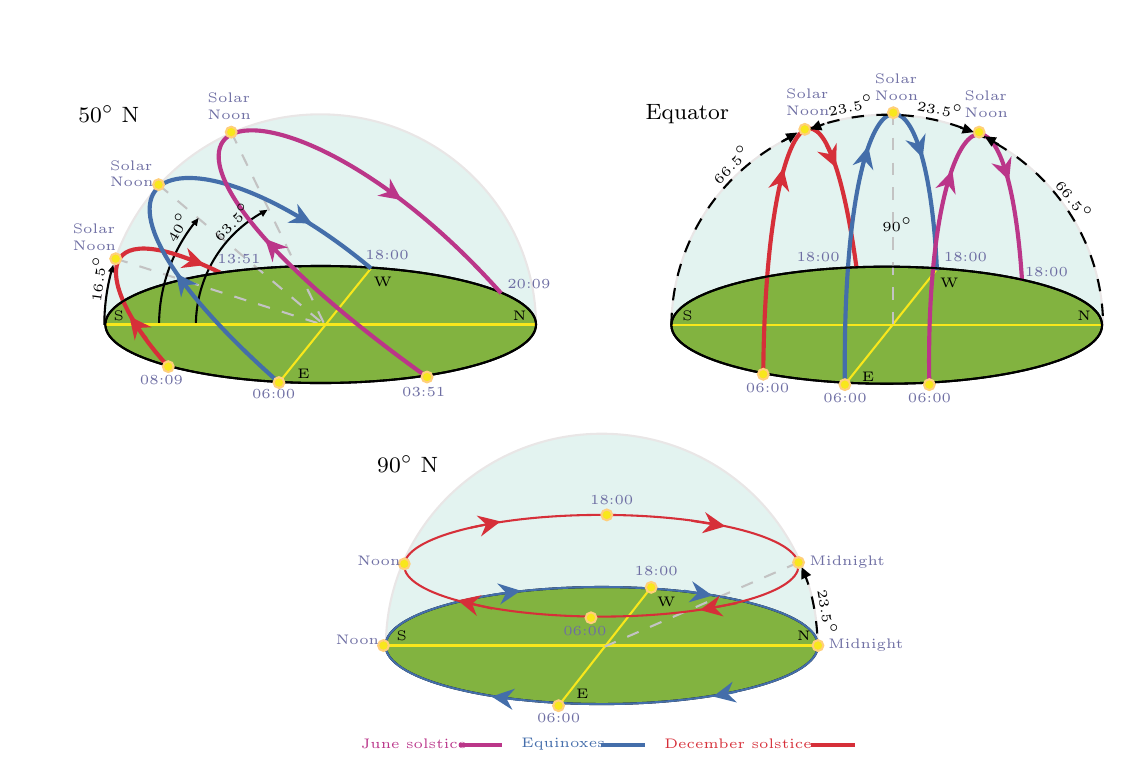
\begin{tikzpicture}[x=0.75pt,y=0.75pt,yscale=-1,xscale=1]
		%uncomment if require: \path (0,1241); %set diagram left start at 0, and has height of 1241
		
		%Shape: Arc [id:dp2422470523146263] 
		\draw  [draw opacity=0][fill={rgb, 255:red, 227; green, 243; blue, 240 }  ,fill opacity=1 ] (224.35,314.06) .. controls (224.69,257.99) and (271.12,212.64) .. (328.34,212.64) .. controls (385.52,212.64) and (431.91,257.91) .. (432.34,313.91) -- (328.34,314.69) -- cycle ; \draw  [color={rgb, 255:red, 233; green, 230; blue, 230 }  ,draw opacity=1 ] (224.35,314.06) .. controls (224.69,257.99) and (271.12,212.64) .. (328.34,212.64) .. controls (385.52,212.64) and (431.91,257.91) .. (432.34,313.91) ;  
		%Shape: Arc [id:dp679483804015613] 
		\draw  [draw opacity=0][fill={rgb, 255:red, 227; green, 243; blue, 240 }  ,fill opacity=1 ] (361.89,160.36) .. controls (362.24,104.29) and (408.67,58.94) .. (465.89,58.94) .. controls (523.07,58.94) and (569.46,104.21) .. (569.89,160.21) -- (465.89,160.99) -- cycle ; \draw  [color={rgb, 255:red, 233; green, 230; blue, 230 }  ,draw opacity=1 ] (361.89,160.36) .. controls (362.24,104.29) and (408.67,58.94) .. (465.89,58.94) .. controls (523.07,58.94) and (569.46,104.21) .. (569.89,160.21) ;  
		%Shape: Arc [id:dp6579991320352137] 
		\draw  [draw opacity=0][fill={rgb, 255:red, 227; green, 243; blue, 240 }  ,fill opacity=1 ] (88.68,160.17) .. controls (89.03,104.1) and (135.46,58.75) .. (192.68,58.75) .. controls (249.85,58.75) and (296.25,104.02) .. (296.68,160.02) -- (192.68,160.8) -- cycle ; \draw  [color={rgb, 255:red, 233; green, 230; blue, 230 }  ,draw opacity=1 ] (88.68,160.17) .. controls (89.03,104.1) and (135.46,58.75) .. (192.68,58.75) .. controls (249.85,58.75) and (296.25,104.02) .. (296.68,160.02) ;  
		%Shape: Ellipse [id:dp026599170011748274] 
		\draw  [fill={rgb, 255:red, 130; green, 179; blue, 64 }  ,fill opacity=1 ] (89.18,160.02) .. controls (89.18,144.45) and (135.63,131.82) .. (192.93,131.82) .. controls (250.23,131.82) and (296.68,144.45) .. (296.68,160.02) .. controls (296.68,175.6) and (250.23,188.22) .. (192.93,188.22) .. controls (135.63,188.22) and (89.18,175.6) .. (89.18,160.02) -- cycle ;
		%Shape: Ellipse [id:dp034852899805606574] 
		\draw  [fill={rgb, 255:red, 130; green, 179; blue, 64 }  ,fill opacity=1 ] (224.18,314.69) .. controls (224.18,299.12) and (270.82,286.49) .. (328.34,286.49) .. controls (385.87,286.49) and (432.5,299.12) .. (432.5,314.69) .. controls (432.5,330.26) and (385.87,342.89) .. (328.34,342.89) .. controls (270.82,342.89) and (224.18,330.26) .. (224.18,314.69) -- cycle ;
		%Shape: Ellipse [id:dp9672961315748498] 
		\draw  [fill={rgb, 255:red, 130; green, 179; blue, 64 }  ,fill opacity=1 ] (361.89,160.36) .. controls (361.89,144.78) and (408.34,132.16) .. (465.64,132.16) .. controls (522.94,132.16) and (569.39,144.78) .. (569.39,160.36) .. controls (569.39,175.93) and (522.94,188.56) .. (465.64,188.56) .. controls (408.34,188.56) and (361.89,175.93) .. (361.89,160.36) -- cycle ;
		%Straight Lines [id:da0645452618745832] 
		\draw [color={rgb, 255:red, 248; green, 231; blue, 28 }  ,draw opacity=1 ]   (172.82,187.99) -- (217.17,132.95) ;
		%Straight Lines [id:da29828143210745206] 
		\draw [color={rgb, 255:red, 248; green, 231; blue, 28 }  ,draw opacity=1 ]   (569.39,160.36) -- (361.89,160.36) ;
		%Straight Lines [id:da562077120077852] 
		\draw [color={rgb, 255:red, 248; green, 231; blue, 28 }  ,draw opacity=1 ]   (432.09,314.69) -- (224.6,314.69) ;
		%Straight Lines [id:da701717847578891] 
		\draw [color={rgb, 255:red, 248; green, 231; blue, 28 }  ,draw opacity=1 ]   (352.15,286.66) -- (307.52,343.69) ;
		%Straight Lines [id:da28752370197924626] 
		\draw [color={rgb, 255:red, 248; green, 231; blue, 28 }  ,draw opacity=1 ]   (490.17,132.95) -- (445.48,188.99) ;
		%Straight Lines [id:da9169139913110784] 
		\draw [color={rgb, 255:red, 187; green, 54; blue, 137 }  ,draw opacity=1 ][line width=1.5]    (259.53,362.6) -- (280.44,362.6) ;
		%Straight Lines [id:da9765715724383317] 
		\draw [color={rgb, 255:red, 68; green, 110; blue, 170 }  ,draw opacity=1 ][line width=1.5]    (328.2,362.6) -- (349.11,362.6) ;
		%Straight Lines [id:da40419882056594303] 
		\draw [color={rgb, 255:red, 214; green, 47; blue, 57 }  ,draw opacity=1 ][line width=1.5]    (429.2,362.6) -- (450.11,362.6) ;
		%Straight Lines [id:da6057738448347012] 
		\draw [color={rgb, 255:red, 195; green, 195; blue, 195 }  ,draw opacity=1 ] [dash pattern={on 4.5pt off 4.5pt}]  (94.15,128.32) -- (194.99,160.47) ;
		%Straight Lines [id:da4733118370839784] 
		\draw [color={rgb, 255:red, 195; green, 195; blue, 195 }  ,draw opacity=1 ] [dash pattern={on 4.5pt off 4.5pt}]  (114.82,92.66) -- (194.99,160.47) ;
		%Straight Lines [id:da5526355665884131] 
		\draw [color={rgb, 255:red, 195; green, 195; blue, 195 }  ,draw opacity=1 ] [dash pattern={on 4.5pt off 4.5pt}]  (149.82,67.32) -- (194.99,160.47) ;
		%Straight Lines [id:da7612642235310549] 
		\draw [color={rgb, 255:red, 195; green, 195; blue, 195 }  ,draw opacity=1 ] [dash pattern={on 4.5pt off 4.5pt}]  (468.82,57.99) -- (468.82,159.98) ;
		%Straight Lines [id:da33292480156237203] 
		\draw [color={rgb, 255:red, 195; green, 195; blue, 195 }  ,draw opacity=1 ] [dash pattern={on 4.5pt off 4.5pt}]  (423.15,274.66) -- (329.83,315.17) ;
		%Curve Lines [id:da7961132204705399] 
		\draw [color={rgb, 255:red, 214; green, 47; blue, 57 }  ,draw opacity=1 ][line width=1.5]    (406.15,183.99) .. controls (407.08,60.34) and (435.41,18.01) .. (451.08,132.67) ;
		%Curve Lines [id:da02576150997648119] 
		\draw [color={rgb, 255:red, 68; green, 110; blue, 170 }  ,draw opacity=1 ][line width=1.5]    (445.48,188.99) .. controls (443.66,33.01) and (484.66,19.67) .. (489.84,133.95) ;
		%Curve Lines [id:da08549260331452802] 
		\draw [color={rgb, 255:red, 187; green, 54; blue, 137 }  ,draw opacity=1 ][line width=1.5]    (486.15,188.99) .. controls (483.66,58.67) and (523.32,21.67) .. (530.84,138.95) ;
		%Shape: Ellipse [id:dp25474571226905507] 
		\draw  [color={rgb, 255:red, 68; green, 110; blue, 170 }  ,draw opacity=1 ] (224.18,314.69) .. controls (224.18,299.12) and (270.82,286.49) .. (328.34,286.49) .. controls (385.87,286.49) and (432.5,299.12) .. (432.5,314.69) .. controls (432.5,330.26) and (385.87,342.89) .. (328.34,342.89) .. controls (270.82,342.89) and (224.18,330.26) .. (224.18,314.69) -- cycle ;
		%Shape: Ellipse [id:dp570098210916735] 
		\draw   (361.89,160.36) .. controls (361.89,144.78) and (408.34,132.16) .. (465.64,132.16) .. controls (522.94,132.16) and (569.39,144.78) .. (569.39,160.36) .. controls (569.39,175.93) and (522.94,188.56) .. (465.64,188.56) .. controls (408.34,188.56) and (361.89,175.93) .. (361.89,160.36) -- cycle ;
		%Shape: Ellipse [id:dp9029901288012265] 
		\draw  [color={rgb, 255:red, 214; green, 47; blue, 57 }  ,draw opacity=1 ] (233.18,276.25) .. controls (233.18,262.72) and (275.71,251.75) .. (328.17,251.75) .. controls (380.62,251.75) and (423.15,262.72) .. (423.15,276.25) .. controls (423.15,289.78) and (380.62,300.75) .. (328.17,300.75) .. controls (275.71,300.75) and (233.18,289.78) .. (233.18,276.25) -- cycle ;
		%Shape: Circle [id:dp3517316942078872] 
		\draw  [color={rgb, 255:red, 255; green, 207; blue, 123 }  ,draw opacity=1 ][fill={rgb, 255:red, 248; green, 231; blue, 28 }  ,fill opacity=1 ] (220.59,314.69) .. controls (220.59,313.26) and (221.75,312.09) .. (223.18,312.09) .. controls (224.62,312.09) and (225.78,313.26) .. (225.78,314.69) .. controls (225.78,316.12) and (224.62,317.29) .. (223.18,317.29) .. controls (221.75,317.29) and (220.59,316.12) .. (220.59,314.69) -- cycle ;
		%Shape: Circle [id:dp47946994544182586] 
		\draw  [color={rgb, 255:red, 255; green, 207; blue, 123 }  ,draw opacity=1 ][fill={rgb, 255:red, 248; green, 231; blue, 28 }  ,fill opacity=1 ] (230.59,275.36) .. controls (230.59,273.92) and (231.75,272.76) .. (233.18,272.76) .. controls (234.62,272.76) and (235.78,273.92) .. (235.78,275.36) .. controls (235.78,276.79) and (234.62,277.95) .. (233.18,277.95) .. controls (231.75,277.95) and (230.59,276.79) .. (230.59,275.36) -- cycle ;
		%Shape: Circle [id:dp16392995495771556] 
		\draw  [color={rgb, 255:red, 255; green, 207; blue, 123 }  ,draw opacity=1 ][fill={rgb, 255:red, 248; green, 231; blue, 28 }  ,fill opacity=1 ] (328.17,251.75) .. controls (328.17,250.32) and (329.33,249.16) .. (330.76,249.16) .. controls (332.2,249.16) and (333.36,250.32) .. (333.36,251.75) .. controls (333.36,253.19) and (332.2,254.35) .. (330.76,254.35) .. controls (329.33,254.35) and (328.17,253.19) .. (328.17,251.75) -- cycle ;
		%Shape: Circle [id:dp9456638416024103] 
		\draw  [color={rgb, 255:red, 255; green, 207; blue, 123 }  ,draw opacity=1 ][fill={rgb, 255:red, 248; green, 231; blue, 28 }  ,fill opacity=1 ] (320.55,301.32) .. controls (320.55,299.89) and (321.72,298.73) .. (323.15,298.73) .. controls (324.58,298.73) and (325.75,299.89) .. (325.75,301.32) .. controls (325.75,302.76) and (324.58,303.92) .. (323.15,303.92) .. controls (321.72,303.92) and (320.55,302.76) .. (320.55,301.32) -- cycle ;
		%Shape: Circle [id:dp9124279427944493] 
		\draw  [color={rgb, 255:red, 255; green, 207; blue, 123 }  ,draw opacity=1 ][fill={rgb, 255:red, 248; green, 231; blue, 28 }  ,fill opacity=1 ] (304.92,343.69) .. controls (304.92,342.26) and (306.08,341.09) .. (307.52,341.09) .. controls (308.95,341.09) and (310.11,342.26) .. (310.11,343.69) .. controls (310.11,345.12) and (308.95,346.29) .. (307.52,346.29) .. controls (306.08,346.29) and (304.92,345.12) .. (304.92,343.69) -- cycle ;
		%Shape: Circle [id:dp12043871542643547] 
		\draw  [color={rgb, 255:red, 255; green, 207; blue, 123 }  ,draw opacity=1 ][fill={rgb, 255:red, 248; green, 231; blue, 28 }  ,fill opacity=1 ] (349.55,286.66) .. controls (349.55,285.22) and (350.72,284.06) .. (352.15,284.06) .. controls (353.58,284.06) and (354.75,285.22) .. (354.75,286.66) .. controls (354.75,288.09) and (353.58,289.25) .. (352.15,289.25) .. controls (350.72,289.25) and (349.55,288.09) .. (349.55,286.66) -- cycle ;
		%Shape: Circle [id:dp8187927743897103] 
		\draw  [color={rgb, 255:red, 255; green, 207; blue, 123 }  ,draw opacity=1 ][fill={rgb, 255:red, 248; green, 231; blue, 28 }  ,fill opacity=1 ] (429.91,314.69) .. controls (429.91,313.26) and (431.07,312.09) .. (432.5,312.09) .. controls (433.94,312.09) and (435.1,313.26) .. (435.1,314.69) .. controls (435.1,316.12) and (433.94,317.29) .. (432.5,317.29) .. controls (431.07,317.29) and (429.91,316.12) .. (429.91,314.69) -- cycle ;
		%Shape: Circle [id:dp24405764600998858] 
		\draw  [color={rgb, 255:red, 255; green, 207; blue, 123 }  ,draw opacity=1 ][fill={rgb, 255:red, 248; green, 231; blue, 28 }  ,fill opacity=1 ] (403.55,183.99) .. controls (403.55,182.56) and (404.72,181.39) .. (406.15,181.39) .. controls (407.58,181.39) and (408.75,182.56) .. (408.75,183.99) .. controls (408.75,185.42) and (407.58,186.59) .. (406.15,186.59) .. controls (404.72,186.59) and (403.55,185.42) .. (403.55,183.99) -- cycle ;
		%Shape: Circle [id:dp06143166039455128] 
		\draw  [color={rgb, 255:red, 255; green, 207; blue, 123 }  ,draw opacity=1 ][fill={rgb, 255:red, 248; green, 231; blue, 28 }  ,fill opacity=1 ] (442.89,188.99) .. controls (442.89,187.56) and (444.05,186.39) .. (445.48,186.39) .. controls (446.92,186.39) and (448.08,187.56) .. (448.08,188.99) .. controls (448.08,190.42) and (446.92,191.59) .. (445.48,191.59) .. controls (444.05,191.59) and (442.89,190.42) .. (442.89,188.99) -- cycle ;
		%Shape: Circle [id:dp3505657865005942] 
		\draw  [color={rgb, 255:red, 255; green, 207; blue, 123 }  ,draw opacity=1 ][fill={rgb, 255:red, 248; green, 231; blue, 28 }  ,fill opacity=1 ] (483.55,188.99) .. controls (483.55,187.56) and (484.72,186.39) .. (486.15,186.39) .. controls (487.58,186.39) and (488.75,187.56) .. (488.75,188.99) .. controls (488.75,190.42) and (487.58,191.59) .. (486.15,191.59) .. controls (484.72,191.59) and (483.55,190.42) .. (483.55,188.99) -- cycle ;
		%Shape: Arc [id:dp5873305968510829] 
		\draw  [draw opacity=0] (132.79,160.39) .. controls (132.82,136.04) and (146.84,114.97) .. (167.25,104.78) -- (194.99,160.47) -- cycle ; \draw    (132.79,160.39) .. controls (132.82,137.01) and (145.74,116.66) .. (164.83,106.05) ; \draw [shift={(167.25,104.78)}, rotate = 148.12] [fill={rgb, 255:red, 0; green, 0; blue, 0 }  ][line width=0.08]  [draw opacity=0] (3.57,-1.72) -- (0,0) -- (3.57,1.72) -- cycle    ; 
		%Shape: Arc [id:dp38657363435695613] 
		\draw  [draw opacity=0] (115.04,160.37) .. controls (115.06,140.7) and (122.19,122.7) .. (133.99,108.78) -- (194.99,160.47) -- cycle ; \draw    (115.04,160.37) .. controls (115.06,141.69) and (121.49,124.5) .. (132.25,110.9) ; \draw [shift={(133.99,108.78)}, rotate = 126.2] [fill={rgb, 255:red, 0; green, 0; blue, 0 }  ][line width=0.08]  [draw opacity=0] (3.57,-1.72) -- (0,0) -- (3.57,1.72) -- cycle    ; 
		%Shape: Arc [id:dp690824190882209] 
		\draw  [draw opacity=0] (88.68,160.17) .. controls (88.69,150.13) and (90.19,140.43) .. (92.95,131.29) -- (188.71,160.29) -- cycle ; \draw    (88.68,160.17) .. controls (88.69,151.13) and (89.9,142.37) .. (92.16,134.05) ; \draw [shift={(92.95,131.29)}, rotate = 103.43] [fill={rgb, 255:red, 0; green, 0; blue, 0 }  ][line width=0.08]  [draw opacity=0] (3.57,-1.72) -- (0,0) -- (3.57,1.72) -- cycle    ; 
		%Straight Lines [id:da4563209144085123] 
		\draw [color={rgb, 255:red, 248; green, 231; blue, 28 }  ,draw opacity=1 ]   (89.18,160.02) -- (296.68,160.02) ;
		%Curve Lines [id:da42699598834552277] 
		\draw [color={rgb, 255:red, 214; green, 47; blue, 57 }  ,draw opacity=1 ][line width=1.5]    (119.48,180.32) .. controls (84.75,141.95) and (79.75,103.61) .. (144.41,134.98) ;
		%Shape: Ellipse [id:dp6059591061934837] 
		\draw   (89.18,160.02) .. controls (89.18,144.45) and (135.63,131.82) .. (192.93,131.82) .. controls (250.23,131.82) and (296.68,144.45) .. (296.68,160.02) .. controls (296.68,175.6) and (250.23,188.22) .. (192.93,188.22) .. controls (135.63,188.22) and (89.18,175.6) .. (89.18,160.02) -- cycle ;
		%Shape: Circle [id:dp3712409213214478] 
		\draw  [color={rgb, 255:red, 255; green, 207; blue, 123 }  ,draw opacity=1 ][fill={rgb, 255:red, 248; green, 231; blue, 28 }  ,fill opacity=1 ] (116.89,180.32) .. controls (116.89,178.89) and (118.05,177.73) .. (119.48,177.73) .. controls (120.92,177.73) and (122.08,178.89) .. (122.08,180.32) .. controls (122.08,181.76) and (120.92,182.92) .. (119.48,182.92) .. controls (118.05,182.92) and (116.89,181.76) .. (116.89,180.32) -- cycle ;
		%Shape: Circle [id:dp13429058818190365] 
		\draw  [color={rgb, 255:red, 255; green, 207; blue, 123 }  ,draw opacity=1 ][fill={rgb, 255:red, 248; green, 231; blue, 28 }  ,fill opacity=1 ] (91.55,128.32) .. controls (91.55,126.89) and (92.72,125.73) .. (94.15,125.73) .. controls (95.58,125.73) and (96.75,126.89) .. (96.75,128.32) .. controls (96.75,129.76) and (95.58,130.92) .. (94.15,130.92) .. controls (92.72,130.92) and (91.55,129.76) .. (91.55,128.32) -- cycle ;
		%Shape: Arc [id:dp9269885967361307] 
		\draw  [draw opacity=0][dash pattern={on 4.5pt off 4.5pt}] (361.89,160.36) .. controls (362.24,104.29) and (408.67,58.94) .. (465.89,58.94) .. controls (523.07,58.94) and (569.46,104.21) .. (569.89,160.21) -- (465.89,160.99) -- cycle ; \draw  [color={rgb, 255:red, 0; green, 0; blue, 0 }  ,draw opacity=1 ][dash pattern={on 4.5pt off 4.5pt}] (361.89,160.36) .. controls (362.24,104.29) and (408.67,58.94) .. (465.89,58.94) .. controls (523.07,58.94) and (569.46,104.21) .. (569.89,160.21) ;  
		%Shape: Circle [id:dp6632792136940118] 
		\draw  [color={rgb, 255:red, 255; green, 207; blue, 123 }  ,draw opacity=1 ][fill={rgb, 255:red, 248; green, 231; blue, 28 }  ,fill opacity=1 ] (423.55,65.99) .. controls (423.55,64.56) and (424.72,63.39) .. (426.15,63.39) .. controls (427.58,63.39) and (428.75,64.56) .. (428.75,65.99) .. controls (428.75,67.42) and (427.58,68.59) .. (426.15,68.59) .. controls (424.72,68.59) and (423.55,67.42) .. (423.55,65.99) -- cycle ;
		%Shape: Circle [id:dp7476666993877557] 
		\draw  [color={rgb, 255:red, 255; green, 207; blue, 123 }  ,draw opacity=1 ][fill={rgb, 255:red, 248; green, 231; blue, 28 }  ,fill opacity=1 ] (466.22,57.99) .. controls (466.22,56.56) and (467.38,55.39) .. (468.82,55.39) .. controls (470.25,55.39) and (471.41,56.56) .. (471.41,57.99) .. controls (471.41,59.42) and (470.25,60.59) .. (468.82,60.59) .. controls (467.38,60.59) and (466.22,59.42) .. (466.22,57.99) -- cycle ;
		%Shape: Circle [id:dp2616436491639995] 
		\draw  [color={rgb, 255:red, 255; green, 207; blue, 123 }  ,draw opacity=1 ][fill={rgb, 255:red, 248; green, 231; blue, 28 }  ,fill opacity=1 ] (507.55,67.32) .. controls (507.55,65.89) and (508.72,64.73) .. (510.15,64.73) .. controls (511.58,64.73) and (512.75,65.89) .. (512.75,67.32) .. controls (512.75,68.76) and (511.58,69.92) .. (510.15,69.92) .. controls (508.72,69.92) and (507.55,68.76) .. (507.55,67.32) -- cycle ;
		%Curve Lines [id:da8436277595173716] 
		\draw  [dash pattern={on 4.5pt off 4.5pt}]  (425.81,279.7) .. controls (429.77,289.11) and (431.89,300.15) .. (432.5,314.69) ;
		\draw [shift={(424.58,276.96)}, rotate = 64.59] [fill={rgb, 255:red, 0; green, 0; blue, 0 }  ][line width=0.08]  [draw opacity=0] (5.36,-2.57) -- (0,0) -- (5.36,2.57) -- cycle    ;
		%Shape: Circle [id:dp2188763011824284] 
		\draw  [color={rgb, 255:red, 255; green, 207; blue, 123 }  ,draw opacity=1 ][fill={rgb, 255:red, 248; green, 231; blue, 28 }  ,fill opacity=1 ] (420.55,274.66) .. controls (420.55,273.22) and (421.72,272.06) .. (423.15,272.06) .. controls (424.58,272.06) and (425.75,273.22) .. (425.75,274.66) .. controls (425.75,276.09) and (424.58,277.25) .. (423.15,277.25) .. controls (421.72,277.25) and (420.55,276.09) .. (420.55,274.66) -- cycle ;
		%Straight Lines [id:da5632576076069373] 
		\draw    (415.83,71.55) -- (420,69.08) ;
		\draw [shift={(422.58,67.55)}, rotate = 149.35] [fill={rgb, 255:red, 0; green, 0; blue, 0 }  ][line width=0.08]  [draw opacity=0] (5.36,-2.57) -- (0,0) -- (5.36,2.57) -- cycle    ;
		%Straight Lines [id:da6279801720440279] 
		\draw    (435.58,63.37) -- (431.55,64.92) ;
		\draw [shift={(428.75,65.99)}, rotate = 339.02] [fill={rgb, 255:red, 0; green, 0; blue, 0 }  ][line width=0.08]  [draw opacity=0] (5.36,-2.57) -- (0,0) -- (5.36,2.57) -- cycle    ;
		%Straight Lines [id:da2516560862804338] 
		\draw    (501.08,65.12) -- (504.71,66.36) ;
		\draw [shift={(507.55,67.32)}, rotate = 198.81] [fill={rgb, 255:red, 0; green, 0; blue, 0 }  ][line width=0.08]  [draw opacity=0] (5.36,-2.57) -- (0,0) -- (5.36,2.57) -- cycle    ;
		%Straight Lines [id:da2491262183137668] 
		\draw    (519.58,73.37) -- (515.41,70.9) ;
		\draw [shift={(512.83,69.37)}, rotate = 30.65] [fill={rgb, 255:red, 0; green, 0; blue, 0 }  ][line width=0.08]  [draw opacity=0] (5.36,-2.57) -- (0,0) -- (5.36,2.57) -- cycle    ;
		%Straight Lines [id:da33711193576536713] 
		\draw [color={rgb, 255:red, 214; green, 47; blue, 57 }  ,draw opacity=1 ][line width=0.75]    (393.59,294.25) -- (378.54,297.04) ;
		\draw [shift={(375.59,297.58)}, rotate = 349.51] [fill={rgb, 255:red, 214; green, 47; blue, 57 }  ,fill opacity=1 ][line width=0.08]  [draw opacity=0] (10.72,-5.15) -- (0,0) -- (10.72,5.15) -- (7.12,0) -- cycle    ;
		%Straight Lines [id:da7541174766087777] 
		\draw [color={rgb, 255:red, 214; green, 47; blue, 57 }  ,draw opacity=1 ][line width=0.75]    (275.59,296.91) -- (261.85,293.61) ;
		\draw [shift={(258.93,292.91)}, rotate = 13.5] [fill={rgb, 255:red, 214; green, 47; blue, 57 }  ,fill opacity=1 ][line width=0.08]  [draw opacity=0] (10.72,-5.15) -- (0,0) -- (10.72,5.15) -- (7.12,0) -- cycle    ;
		%Straight Lines [id:da6200964489759901] 
		\draw [color={rgb, 255:red, 214; green, 47; blue, 57 }  ,draw opacity=1 ][line width=0.75]    (265.26,257.91) -- (276.66,255.53) ;
		\draw [shift={(279.59,254.91)}, rotate = 168.18] [fill={rgb, 255:red, 214; green, 47; blue, 57 }  ,fill opacity=1 ][line width=0.08]  [draw opacity=0] (10.72,-5.15) -- (0,0) -- (10.72,5.15) -- (7.12,0) -- cycle    ;
		%Straight Lines [id:da42864157492109034] 
		\draw [color={rgb, 255:red, 214; green, 47; blue, 57 }  ,draw opacity=1 ][line width=0.75]    (371.59,254.58) -- (384.97,256.76) ;
		\draw [shift={(387.93,257.25)}, rotate = 189.27] [fill={rgb, 255:red, 214; green, 47; blue, 57 }  ,fill opacity=1 ][line width=0.08]  [draw opacity=0] (10.72,-5.15) -- (0,0) -- (10.72,5.15) -- (7.12,0) -- cycle    ;
		%Straight Lines [id:da47006704908737396] 
		\draw [color={rgb, 255:red, 214; green, 47; blue, 57 }  ,draw opacity=1 ][line width=0.75]    (109.26,166.91) -- (102.62,158.43) ;
		\draw [shift={(100.78,156.07)}, rotate = 51.97] [fill={rgb, 255:red, 214; green, 47; blue, 57 }  ,fill opacity=1 ][line width=0.08]  [draw opacity=0] (10.72,-5.15) -- (0,0) -- (10.72,5.15) -- (7.12,0) -- cycle    ;
		%Straight Lines [id:da5344433009658485] 
		\draw [color={rgb, 255:red, 214; green, 47; blue, 57 }  ,draw opacity=1 ][line width=0.75]    (124.93,127.25) -- (134.27,130.43) ;
		\draw [shift={(137.11,131.4)}, rotate = 198.82] [fill={rgb, 255:red, 214; green, 47; blue, 57 }  ,fill opacity=1 ][line width=0.08]  [draw opacity=0] (10.72,-5.15) -- (0,0) -- (10.72,5.15) -- (7.12,0) -- cycle    ;
		%Curve Lines [id:da08444480231313056] 
		\draw [color={rgb, 255:red, 68; green, 110; blue, 170 }  ,draw opacity=1 ][line width=1.5]    (172.82,187.99) .. controls (52.75,81.61) and (127.75,58.28) .. (217.17,132.95) ;
		%Curve Lines [id:da3050864468318677] 
		\draw [color={rgb, 255:red, 187; green, 54; blue, 137 }  ,draw opacity=1 ][line width=1.5]    (244.15,185.32) .. controls (56.75,51.34) and (168.99,20.67) .. (279.84,144.95) ;
		%Shape: Circle [id:dp655057149862863] 
		\draw  [color={rgb, 255:red, 255; green, 207; blue, 123 }  ,draw opacity=1 ][fill={rgb, 255:red, 248; green, 231; blue, 28 }  ,fill opacity=1 ] (170.22,187.99) .. controls (170.22,186.56) and (171.38,185.39) .. (172.82,185.39) .. controls (174.25,185.39) and (175.41,186.56) .. (175.41,187.99) .. controls (175.41,189.42) and (174.25,190.59) .. (172.82,190.59) .. controls (171.38,190.59) and (170.22,189.42) .. (170.22,187.99) -- cycle ;
		%Shape: Circle [id:dp9656764333019969] 
		\draw  [color={rgb, 255:red, 255; green, 207; blue, 123 }  ,draw opacity=1 ][fill={rgb, 255:red, 248; green, 231; blue, 28 }  ,fill opacity=1 ] (241.55,185.32) .. controls (241.55,183.89) and (242.72,182.73) .. (244.15,182.73) .. controls (245.58,182.73) and (246.75,183.89) .. (246.75,185.32) .. controls (246.75,186.76) and (245.58,187.92) .. (244.15,187.92) .. controls (242.72,187.92) and (241.55,186.76) .. (241.55,185.32) -- cycle ;
		%Shape: Circle [id:dp14536176964778158] 
		\draw  [color={rgb, 255:red, 255; green, 207; blue, 123 }  ,draw opacity=1 ][fill={rgb, 255:red, 248; green, 231; blue, 28 }  ,fill opacity=1 ] (112.22,92.66) .. controls (112.22,91.22) and (113.38,90.06) .. (114.82,90.06) .. controls (116.25,90.06) and (117.41,91.22) .. (117.41,92.66) .. controls (117.41,94.09) and (116.25,95.25) .. (114.82,95.25) .. controls (113.38,95.25) and (112.22,94.09) .. (112.22,92.66) -- cycle ;
		%Shape: Circle [id:dp5939615740183428] 
		\draw  [color={rgb, 255:red, 255; green, 207; blue, 123 }  ,draw opacity=1 ][fill={rgb, 255:red, 248; green, 231; blue, 28 }  ,fill opacity=1 ] (147.22,67.32) .. controls (147.22,65.89) and (148.38,64.73) .. (149.82,64.73) .. controls (151.25,64.73) and (152.41,65.89) .. (152.41,67.32) .. controls (152.41,68.76) and (151.25,69.92) .. (149.82,69.92) .. controls (148.38,69.92) and (147.22,68.76) .. (147.22,67.32) -- cycle ;
		%Straight Lines [id:da3799597642654473] 
		\draw [color={rgb, 255:red, 214; green, 47; blue, 57 }  ,draw opacity=1 ][line width=0.75]    (413.59,95.4) -- (415.18,87.67) ;
		\draw [shift={(415.78,84.73)}, rotate = 101.56] [fill={rgb, 255:red, 214; green, 47; blue, 57 }  ,fill opacity=1 ][line width=0.08]  [draw opacity=0] (10.72,-5.15) -- (0,0) -- (10.72,5.15) -- (7.12,0) -- cycle    ;
		%Straight Lines [id:da2713616608158589] 
		\draw [color={rgb, 255:red, 214; green, 47; blue, 57 }  ,draw opacity=1 ][line width=0.75]    (436.26,73.4) -- (440.02,81.67) ;
		\draw [shift={(441.26,84.4)}, rotate = 245.56] [fill={rgb, 255:red, 214; green, 47; blue, 57 }  ,fill opacity=1 ][line width=0.08]  [draw opacity=0] (10.72,-5.15) -- (0,0) -- (10.72,5.15) -- (7.12,0) -- cycle    ;
		%Straight Lines [id:da037783389534803424] 
		\draw [color={rgb, 255:red, 68; green, 110; blue, 170 }  ,draw opacity=1 ][line width=0.75]    (131.59,146.25) -- (124.96,137.76) ;
		\draw [shift={(123.11,135.4)}, rotate = 51.97] [fill={rgb, 255:red, 68; green, 110; blue, 170 }  ,fill opacity=1 ][line width=0.08]  [draw opacity=0] (10.72,-5.15) -- (0,0) -- (10.72,5.15) -- (7.12,0) -- cycle    ;
		%Straight Lines [id:da02921293626575916] 
		\draw [color={rgb, 255:red, 68; green, 110; blue, 170 }  ,draw opacity=1 ][line width=0.75]    (176.05,104.73) -- (186.06,110) ;
		\draw [shift={(188.72,111.4)}, rotate = 207.76] [fill={rgb, 255:red, 68; green, 110; blue, 170 }  ,fill opacity=1 ][line width=0.08]  [draw opacity=0] (10.72,-5.15) -- (0,0) -- (10.72,5.15) -- (7.12,0) -- cycle    ;
		%Straight Lines [id:da0976162170960242] 
		\draw [color={rgb, 255:red, 68; green, 110; blue, 170 }  ,draw opacity=1 ][line width=0.75]    (453.05,89.07) -- (456,76.98) ;
		\draw [shift={(456.72,74.07)}, rotate = 103.74] [fill={rgb, 255:red, 68; green, 110; blue, 170 }  ,fill opacity=1 ][line width=0.08]  [draw opacity=0] (10.72,-5.15) -- (0,0) -- (10.72,5.15) -- (7.12,0) -- cycle    ;
		%Straight Lines [id:da17055383800295876] 
		\draw [color={rgb, 255:red, 68; green, 110; blue, 170 }  ,draw opacity=1 ][line width=0.75]    (478.96,68.07) -- (481.99,76.9) ;
		\draw [shift={(482.96,79.73)}, rotate = 251.08] [fill={rgb, 255:red, 68; green, 110; blue, 170 }  ,fill opacity=1 ][line width=0.08]  [draw opacity=0] (10.72,-5.15) -- (0,0) -- (10.72,5.15) -- (7.12,0) -- cycle    ;
		%Straight Lines [id:da1965718168063728] 
		\draw [color={rgb, 255:red, 68; green, 110; blue, 170 }  ,draw opacity=1 ][line width=0.75]    (393.29,336.95) -- (384.9,338.67) ;
		\draw [shift={(381.96,339.28)}, rotate = 348.37] [fill={rgb, 255:red, 68; green, 110; blue, 170 }  ,fill opacity=1 ][line width=0.08]  [draw opacity=0] (10.72,-5.15) -- (0,0) -- (10.72,5.15) -- (7.12,0) -- cycle    ;
		%Straight Lines [id:da023257054618457396] 
		\draw [color={rgb, 255:red, 68; green, 110; blue, 170 }  ,draw opacity=1 ][line width=0.75]    (288.96,340.95) -- (278.27,339.64) ;
		\draw [shift={(275.29,339.28)}, rotate = 6.95] [fill={rgb, 255:red, 68; green, 110; blue, 170 }  ,fill opacity=1 ][line width=0.08]  [draw opacity=0] (10.72,-5.15) -- (0,0) -- (10.72,5.15) -- (7.12,0) -- cycle    ;
		%Straight Lines [id:da6153811416352519] 
		\draw [color={rgb, 255:red, 68; green, 110; blue, 170 }  ,draw opacity=1 ][line width=0.75]    (275.62,290.28) -- (286.32,288.71) ;
		\draw [shift={(289.29,288.28)}, rotate = 171.67] [fill={rgb, 255:red, 68; green, 110; blue, 170 }  ,fill opacity=1 ][line width=0.08]  [draw opacity=0] (10.72,-5.15) -- (0,0) -- (10.72,5.15) -- (7.12,0) -- cycle    ;
		%Straight Lines [id:da5084173827924052] 
		\draw [color={rgb, 255:red, 68; green, 110; blue, 170 }  ,draw opacity=1 ][line width=0.75]    (367.96,288.28) -- (378.67,290.11) ;
		\draw [shift={(381.62,290.61)}, rotate = 189.69] [fill={rgb, 255:red, 68; green, 110; blue, 170 }  ,fill opacity=1 ][line width=0.08]  [draw opacity=0] (10.72,-5.15) -- (0,0) -- (10.72,5.15) -- (7.12,0) -- cycle    ;
		%Straight Lines [id:da5707264368452845] 
		\draw [color={rgb, 255:red, 187; green, 54; blue, 137 }  ,draw opacity=1 ][line width=0.75]    (175.59,128.7) -- (168.18,120.91) ;
		\draw [shift={(166.11,118.73)}, rotate = 46.43] [fill={rgb, 255:red, 187; green, 54; blue, 137 }  ,fill opacity=1 ][line width=0.08]  [draw opacity=0] (10.72,-5.15) -- (0,0) -- (10.72,5.15) -- (7.12,0) -- cycle    ;
		%Straight Lines [id:da8907337606441528] 
		\draw [color={rgb, 255:red, 187; green, 54; blue, 137 }  ,draw opacity=1 ][line width=0.75]    (221.26,92.37) -- (229.49,98.29) ;
		\draw [shift={(231.93,100.04)}, rotate = 215.71] [fill={rgb, 255:red, 187; green, 54; blue, 137 }  ,fill opacity=1 ][line width=0.08]  [draw opacity=0] (10.72,-5.15) -- (0,0) -- (10.72,5.15) -- (7.12,0) -- cycle    ;
		%Straight Lines [id:da5355419515081008] 
		\draw [color={rgb, 255:red, 187; green, 54; blue, 137 }  ,draw opacity=1 ][line width=0.75]    (492.93,99.04) -- (496.33,88.56) ;
		\draw [shift={(497.26,85.7)}, rotate = 108] [fill={rgb, 255:red, 187; green, 54; blue, 137 }  ,fill opacity=1 ][line width=0.08]  [draw opacity=0] (10.72,-5.15) -- (0,0) -- (10.72,5.15) -- (7.12,0) -- cycle    ;
		%Straight Lines [id:da24750502396292218] 
		\draw [color={rgb, 255:red, 187; green, 54; blue, 137 }  ,draw opacity=1 ][line width=0.75]    (520.59,79.7) -- (523.57,87.88) ;
		\draw [shift={(524.59,90.7)}, rotate = 250.02] [fill={rgb, 255:red, 187; green, 54; blue, 137 }  ,fill opacity=1 ][line width=0.08]  [draw opacity=0] (10.72,-5.15) -- (0,0) -- (10.72,5.15) -- (7.12,0) -- cycle    ;
		
		% Text Node
		\draw (91.67,152) node [anchor=north west][inner sep=0.75pt]  [font=\tiny] [align=left] {S};
		% Text Node
		\draw (228,306) node [anchor=north west][inner sep=0.75pt]  [font=\tiny] [align=left] {S};
		% Text Node
		\draw (365.67,152) node [anchor=north west][inner sep=0.75pt]  [font=\tiny] [align=left] {S};
		% Text Node
		\draw (284,152) node [anchor=north west][inner sep=0.75pt]  [font=\tiny] [align=left] {N};
		% Text Node
		\draw (421,306) node [anchor=north west][inner sep=0.75pt]  [font=\tiny] [align=left] {N};
		% Text Node
		\draw (556,152) node [anchor=north west][inner sep=0.75pt]  [font=\tiny] [align=left] {N};
		% Text Node
		\draw (216.96,135.46) node [anchor=north west][inner sep=0.75pt]  [font=\tiny] [align=left] {W};
		% Text Node
		\draw (489.84,135.95) node [anchor=north west][inner sep=0.75pt]  [font=\tiny] [align=left] {W};
		% Text Node
		\draw (353.55,289.66) node [anchor=north west][inner sep=0.75pt]  [font=\tiny] [align=left] {W};
		% Text Node
		\draw (180.22,180) node [anchor=north west][inner sep=0.75pt]  [font=\tiny] [align=left] {E};
		% Text Node
		\draw (314.55,334) node [anchor=north west][inner sep=0.75pt]  [font=\tiny] [align=left] {E};
		% Text Node
		\draw (74.67,52.88) node [anchor=north west][inner sep=0.75pt]  [font=\footnotesize] [align=left] {$\displaystyle 50^{\circ }$ N};
		% Text Node
		\draw (348,52.55) node [anchor=north west][inner sep=0.75pt]  [font=\small] [align=left] {{\footnotesize Equator}};
		% Text Node
		\draw (218.67,221.63) node [anchor=north west][inner sep=0.75pt]  [font=\footnotesize] [align=left] {$\displaystyle 90^{\circ }$ N};
		% Text Node
		\draw (210.77,358) node [anchor=north west][inner sep=0.75pt]  [font=\tiny] [align=left] {\textcolor[rgb]{0.73,0.21,0.54}{June solstice}};
		% Text Node
		\draw (288.11,358) node [anchor=north west][inner sep=0.75pt]  [font=\tiny] [align=left] {\textcolor[rgb]{0.27,0.43,0.67}{Equinoxes}};
		% Text Node
		\draw (357,358) node [anchor=north west][inner sep=0.75pt]  [font=\tiny,color={rgb, 255:red, 214; green, 47; blue, 57 }  ,opacity=1 ] [align=left] {December solstice};
		% Text Node
		\draw (72,110) node [anchor=north west][inner sep=0.75pt]  [font=\tiny] [align=left] {\textcolor[rgb]{0.43,0.43,0.64}{Solar}\\\textcolor[rgb]{0.43,0.43,0.64}{Noon}};
		% Text Node
		\draw (90,79.46) node [anchor=north west][inner sep=0.75pt]  [font=\tiny] [align=left] {\textcolor[rgb]{0.43,0.43,0.64}{Solar}\\\textcolor[rgb]{0.43,0.43,0.64}{Noon}};
		% Text Node
		\draw (137,47) node [anchor=north west][inner sep=0.75pt]  [font=\tiny] [align=left] {\textcolor[rgb]{0.43,0.43,0.64}{Solar}\\\textcolor[rgb]{0.43,0.43,0.64}{Noon}};
		% Text Node
		\draw (415.71,45) node [anchor=north west][inner sep=0.75pt]  [font=\tiny] [align=left] {\textcolor[rgb]{0.43,0.43,0.64}{Solar}\\\textcolor[rgb]{0.43,0.43,0.64}{Noon}};
		% Text Node
		\draw (458.46,38) node [anchor=north west][inner sep=0.75pt]  [font=\tiny] [align=left] {\textcolor[rgb]{0.43,0.43,0.64}{Solar}\\\textcolor[rgb]{0.43,0.43,0.64}{Noon}};
		% Text Node
		\draw (501.71,46) node [anchor=north west][inner sep=0.75pt]  [font=\tiny] [align=left] {\textcolor[rgb]{0.43,0.43,0.64}{Solar}\\\textcolor[rgb]{0.43,0.43,0.64}{Noon}};
		% Text Node
		\draw (209.05,270) node [anchor=north west][inner sep=0.75pt]  [font=\tiny] [align=left] {\textcolor[rgb]{0.43,0.43,0.64}{Noon}};
		% Text Node
		\draw (198.71,308) node [anchor=north west][inner sep=0.75pt]  [font=\tiny] [align=left] {\textcolor[rgb]{0.43,0.43,0.64}{Noon}};
		% Text Node
		\draw (427.05,270) node [anchor=north west][inner sep=0.75pt]  [font=\tiny] [align=left] {\textcolor[rgb]{0.43,0.43,0.64}{Midnight}};
		% Text Node
		\draw (436,310) node [anchor=north west][inner sep=0.75pt]  [font=\tiny] [align=left] {\textcolor[rgb]{0.43,0.43,0.64}{Midnight}};
		% Text Node
		\draw (230.67,189) node [anchor=north west][inner sep=0.75pt]  [font=\tiny] [align=left] {\textcolor[rgb]{0.43,0.43,0.64}{\NoAutoSpacing 03:51}};
		% Text Node
		\draw (158.33,190) node [anchor=north west][inner sep=0.75pt]  [font=\tiny] [align=left] {\textcolor[rgb]{0.43,0.43,0.64}{\NoAutoSpacing 06:00}};
		% Text Node
		\draw (104.33,183) node [anchor=north west][inner sep=0.75pt]  [font=\tiny] [align=left] {\textcolor[rgb]{0.43,0.43,0.64}{\NoAutoSpacing 08:09}};
		% Text Node
		\draw (141.67,125) node [anchor=north west][inner sep=0.75pt]  [font=\tiny] [align=left] {\textcolor[rgb]{0.43,0.43,0.64}{\NoAutoSpacing 13:51}};
		% Text Node
		\draw (213,123) node [anchor=north west][inner sep=0.75pt]  [font=\tiny] [align=left] {\textcolor[rgb]{0.43,0.43,0.64}{\NoAutoSpacing 18:00}};
		% Text Node
		\draw (281.33,137) node [anchor=north west][inner sep=0.75pt]  [font=\tiny] [align=left] {\textcolor[rgb]{0.43,0.43,0.64}{\NoAutoSpacing 20:09}};
		% Text Node
		\draw (295.67,346) node [anchor=north west][inner sep=0.75pt]  [font=\tiny] [align=left] {\textcolor[rgb]{0.43,0.43,0.64}{\NoAutoSpacing 06:00}};
		% Text Node
		\draw (308.33,304) node [anchor=north west][inner sep=0.75pt]  [font=\tiny] [align=left] {\textcolor[rgb]{0.43,0.43,0.64}{\NoAutoSpacing 06:00}};
		% Text Node
		\draw (342.67,275) node [anchor=north west][inner sep=0.75pt]  [font=\tiny] [align=left] {\textcolor[rgb]{0.43,0.43,0.64}{\NoAutoSpacing 18:00}};
		% Text Node
		\draw (321.25,241) node [anchor=north west][inner sep=0.75pt]  [font=\tiny] [align=left] {\textcolor[rgb]{0.43,0.43,0.64}{\NoAutoSpacing 18:00}};
		% Text Node
		\draw (396.33,187) node [anchor=north west][inner sep=0.75pt]  [font=\tiny] [align=left] {\textcolor[rgb]{0.43,0.43,0.64}{\NoAutoSpacing 06:00}};
		% Text Node
		\draw (433.67,192) node [anchor=north west][inner sep=0.75pt]  [font=\tiny] [align=left] {\textcolor[rgb]{0.43,0.43,0.64}{\NoAutoSpacing 06:00}};
		% Text Node
		\draw (474.33,192) node [anchor=north west][inner sep=0.75pt]  [font=\tiny] [align=left] {\textcolor[rgb]{0.43,0.43,0.64}{\NoAutoSpacing 06:00}};
		% Text Node
		\draw (420.67,124) node [anchor=north west][inner sep=0.75pt]  [font=\tiny] [align=left] {\textcolor[rgb]{0.43,0.43,0.64}{\NoAutoSpacing 18:00}};
		% Text Node
		\draw (491.67,124) node [anchor=north west][inner sep=0.75pt]  [font=\tiny] [align=left] {\textcolor[rgb]{0.43,0.43,0.64}{\NoAutoSpacing 18:00}};
		% Text Node
		\draw (530.67,131) node [anchor=north west][inner sep=0.75pt]  [font=\tiny] [align=left] {\textcolor[rgb]{0.43,0.43,0.64}{\NoAutoSpacing 18:00}};
		% Text Node
		\draw (462,106.88) node [anchor=north west][inner sep=0.75pt]  [font=\tiny] [align=left] {$\displaystyle 90^{\circ }$};
		% Text Node
		\draw (137.55,115.75) node [anchor=north west][inner sep=0.75pt]  [font=\tiny,rotate=-315.72] [align=left] {$\displaystyle 63.5^{\circ }$};
		% Text Node
		\draw (115,117.95) node [anchor=north west][inner sep=0.75pt]  [font=\tiny,rotate=-300.76] [align=left] {$\displaystyle 40^{\circ }$};
		% Text Node
		\draw (78.7,149.88) node [anchor=north west][inner sep=0.75pt]  [font=\tiny,rotate=-277.7] [align=left] {$\displaystyle 16.5^{\circ }$};
		% Text Node
		\draw (378.09,88.17) node [anchor=north west][inner sep=0.75pt]  [font=\tiny,rotate=-314.52] [align=left] {$\displaystyle 66.5^{\circ }$};
		% Text Node
		\draw (435,52) node [anchor=north west][inner sep=0.75pt]  [font=\tiny,rotate=-349] [align=left] {$\displaystyle 23.5^{\circ }$};
		% Text Node
		\draw (480,48.5) node [anchor=north west][inner sep=0.75pt]  [font=\tiny,rotate=-11.18] [align=left] {$\displaystyle 23.5^{\circ }$};
		% Text Node
		\draw (552,86.84) node [anchor=north west][inner sep=0.75pt]  [font=\tiny,rotate=-51.5] [align=left] {$\displaystyle 66.5^{\circ }$};
		% Text Node
		\draw (440,285.2) node [anchor=north west][inner sep=0.75pt]  [font=\tiny,rotate=-80.81] [align=left] {$\displaystyle 23.5^{\circ }$};
		% Text Node
		\draw (452.22,181.64) node [anchor=north west][inner sep=0.75pt]  [font=\tiny] [align=left] {E};
		\end{tikzpicture}
		\vspace*{3mm}
		\caption{Solstices and Equinoxes depending on the latitude}
	\end{figure}
	\end{tcolorbox}
	Obviously, the result we will get here is not complete, since, as we know, we had to wait the development of General Relativity to give the exact value of the perihelion  precession of Mercury (that's why will come back on this subject further below).

	To calculate the effect of precession, we will seek the equivalent of the Binet formulas seen above in relativistic form (we will see the classical form in the section of General Relativity). For this we proceed as follows:

	The relativistic Lagrangian of the system is (\SeeChapter{see section Special Relativity page \pageref{mass energy equivalence}}):
	
	\begin{tcolorbox}[title=Remark,arc=10pt,breakable,drop lifted shadow,
  skin=enhanced,
  skin first is subskin of={enhancedfirst}{arc=10pt,no shadow},
  skin middle is subskin of={enhancedmiddle}{arc=10pt,no shadow},
  skin last is subskin of={enhancedlast}{drop lifted shadow}]
	We subtract then energy at rest because only interest us here the study of the kinetic and potential energy. The potential energy is summed in the Lagrangian above (which is not consistent with the practice) but we will reverse the sign later below during the developments.
	\end{tcolorbox}
	With (\SeeChapter{see section Special Relativity page \pageref{fitzgerald lorentz factor} and Vector Calculus page \pageref{polar coordinates}}):
	
	and the reduce mass for recall:
	
	The angular moment:
	
	in relativistic form and applied to our study is:
	
	Taking the norm, we have without forgetting that in our study $\vec{\omega}\bot\vec{r}$ and therefore $(\vec{\omega}\bot\vec{r})\bot\vec{r}$: 
	
	and let us recall that we have adopted the notation $\omega=\dot{\theta}$ (in case you forget the definition...). Which finally gives us:
	
	To establish the relativistic equivalent of the Binet formulas:
	\begin{itemize}
		\item We deduce the expression of the angular momentum:
		

		\item We seek for a relation of the type $\dot{r}=\dot{r}(\theta)$ (as the trajectory is a conic):
		
		Indeed let us recall that in polar coordinates the speed is given by the following expression (\SeeChapter{see section Vector Calculus page \pageref{polar coordinates}}):
		
		That is to say, $\dot{r}=f(r,\theta)$. The latter expression gives us the possibility to write that:
		
		
		\item We seek a relation of the type $\ddot{r}=\ddot{r}(\theta)$:
		
	\end{itemize}
	From the equations obtained previously, we have successively:
	
	Let us recall that we have defined in special relativity $\beta$ and that by using the speed in polar coordinates:
	
	With the previous relations, this gives us:
	
	On the other hand:
	
	By substituting the prior previous relation in the latter:
	
	By putting $u=1/r$ and as:
	
	The prior-previous relations becomes with this expression:
	
	Equating this relation with that of the Lagrangian:
	
	Differentiating the latter relation relatively to $\theta$:
	
	Indeed, the Lagrangian is constant over time (the system is assumed to be conservative), we then have:
	
	and also:
	
	But if we continue:
	
	By referring to:
	
	So we get:
	
	That gives after a few simplifications:
		
	By multiplying the latter by $\mu^2c^2/b^2$:
	
	In a gravitational potential:
	
	The Binet equation in special relativity is then:
	
	To find a solution to this differential equation, we will group the variable $u$ in the left side:
	
	We put:
	
	The differential equation then can be written:
	
	We put:
	
	By taking the second derivative:
	
	We then get a simple differential equation:
	
	whose solution is well known to us (\SeeChapter{see section Differential and Integral Calculus page \pageref{second order differential equations}}):
	
	What can still be written as $\Omega^2$ is a constant:
	
	with $k_1,k_2=c^{te}$.

	To determine the constants $k_1,k_2$, we place ourselves first in the situation for which $\theta=0$, where $r$ is minimal and therefore by $u$ is maximum by definition.
	
	We derivate relatively to $\theta$:
	
	Therefore $k_2=0$ which makes that the relation:
	
	becomes:
	
	Written differently (trying to return to a similar notation to that of the study of conic) then:
	
	And the interest to write this in this way is to notice that we fall ultimately on the equation of an ellipse with $p$ being the focal parameter of the conic, focal parameter given for recall by (\SeeChapter{see section Analytical Geometry page \pageref{parameter of the ellipse}}):
	
	where $a$ is the half major axes of the ellipse.
	
	Now let us put:
	
	At the first passage through the perihelion $\theta=0$ where:
	
	we have therefore:
	
	At the second passage through the perihelion $\theta=2\pi$, we have:
	
	we also have:
	
	The trajectory is still an ellipse but the angle $\Omega\theta_0$ that was zero initially has become $\Omega\theta_1=2\pi$.

	That is, if we have:
	
	Therefore:
	
	Which gives us:
	
	Since $G^2\ll c^2$, a development in Taylor series give us (\SeeChapter{see section Sequences and Series page \pageref{usual maclaurin developments}}):
	
	By limiting at the order $2$:
	
	So in conclusion, there is an advancement of the perihelion taking place in the satellite's direction of rotation. For a repository located in the satellite's rotation plane, the trajectory is always an ellipse.

	This advance is of:
	
	by period. Either by expliciting the momentum given for reminder by:
	
	It comes after simplification:
	
	We will now allow us a rough approximation (mixture of relativistic and non-relativistic). If we consider the last relation, we have obtained during our developments of the Keplerian orbital trajectories the relation:
	
	Therefore, injecting this into the relation of $\Delta \alpha$	we have:
	
	And we have also proved in the section of Analytical Geometry that:
	
	Therefore:
	
	Unfortunately, the numerical values for Mercury precession with $G=6.674\cdot 10^{-11}\;[\text{m}^3\cdot\text{kg}^{-1}\cdot \text{s}^{-2} ]$, $M=1.99\cdot 10^{30}$ [kg], $e=0.260$, $a=5.787\cdot 10^{10}$ [m] and $T=88$ [days], gives for a century ($100$ years of $365$ days):
	
	Thus a precession of an angle of $7''$ century, and not the $43''$ as expected (...) there is therefore a lack of a factor $6$ that only the General Relativity (\SeeChapter{see section General Relativity page \pageref{general relativity precession of mercury perihelion}}) makes possible to find. It is nevertheless interesting that Special Relativity already gives an orbit that precesses where Newton sees stable ellipse and that this approximation works for all the planets except Mercury (the planet closest to the Sun and undergoing the brunt of curvature of space-time).
	
	A more detailed treatment taking into account that the Sun is not a perfect sphere (even if its the nearest perfect spherical object in the solar system) - there is an average variation of approximately only $6$ kilometres between the equatorial radius and the polar radius of the Sun - also lead to a result that doesn't explain Mercury perihelion precession!
	\begin{tcolorbox}[title=Remark,arc=10pt,breakable,drop lifted shadow,
  skin=enhanced,
  skin first is subskin of={enhancedfirst}{arc=10pt,no shadow},
  skin middle is subskin of={enhancedmiddle}{arc=10pt,no shadow},
  skin last is subskin of={enhancedlast}{drop lifted shadow}]
	By applying exactly the same reasoning to corpuscular quantum physics (electrical potential) but with the ad hoc constants seen in the section of Electrostatics, we find:
	
	with $\vec{b}=\mu\vec{r}\times\vec{v}$ being the momentum and in the case of the atom, we will take (\SeeChapter{see section Corpuscular Quantum Physics page \pageref{second quantification condition}}):
	
	with reduced mass equal to:
	
	\end{tcolorbox}
	If the positions of the perihelion (and therefore the aphelion) of the Earth-Moon center of gravity (whose barycenter is located on average $4,671$ [km] from Earth's center) were constant over time, the duration of the different seasons would be constant. But the orbit of the center of gravity Earth-Moon also rotates in its plane in the forward direction at about 12'' per year (a revolution is about $108,000$ years).

	The precession of the equinox occurs in the opposite direction (retrograde direction) at about $50''$ per year (then a "\NewTerm{precession equinox}\index{precession equinox}" revolution is about $26,000$ years). The combination of these two movements permits to calculate the period of the passage of the perihelion of the Earth by the direction of the vernal equinox, this period of about $21,000$ years and is named the "\NewTerm{climatic precession}\index{climatic precession}.
	\begin{figure}[H]
		\centering
		\resizebox{\textwidth}{!}{%
		\begin{tikzpicture}[>=latex',semithick,auto,remember picture]
		  \node at (-7,0) (o1) {\begin{tikzpicture}[scale=1,>=latex',
		  decoration={markings, mark=at position 0.85 with {\arrow[scale=3]{>} } }]
		  	\draw [fill=cyan!30,opacity=.6,postaction={decorate}] (0,0) ellipse (2.5981 and 3);
			\draw (0,-3) -- (0,3) (-2.25,-1.5) -- (2.25,-1.5);
			\draw [fill=yellow] (0,-1.5) circle (.3);
			\draw [->,red,ultra thick] (-.5,-3) -- (.5,-3);
			\draw [->,red,ultra thick] (-.5,3) -- (.5,3);
			\draw [->,red,ultra thick] (-2.75,-1.5) -- (-1.75,-1.5);
			\draw [->,red,ultra thick] (1.75,-1.5) -- (2.75,-1.5);
			\draw [fill=blue] 
				(0,-3) circle (.2)
				(0,3) circle (.2)
				(-2.25,-1.5) circle (.2)
				(2.25,-1.5) circle (.2);
			\node [text centered] at (-1.2,.8) {Spring};
			\node [text centered] at (1.2,.8) {Winter};
			\node [text centered] at (-1,-2) {Summer};
			\node [text centered] at (1,-2) {Fall};
			\node [text centered, text width=5em] at (0,3.8) {Spring Equinox};
			\node [text centered, text width=5em] at (0,-3.8) {Fall Equinox};
			\node [text centered, text width=5em] at (-3.5,-1.5) {Summer Solstice};
			\node [text centered, text width=5em] at (3.5,-1.5) {Winter Solstice};
			\end{tikzpicture}
			};
		    \node [text centered,text width=16em] at (-7,-4.7) (t1) {\normalsize 5000 years ago and 15000 years from now};
		    \node at (7,0) (o2) {\begin{tikzpicture}[scale=1,>=latex',
		  decoration={markings, mark=at position 0.85 with {\arrow[scale=3]{>} } }]
		  	\draw [fill=cyan!30,opacity=.6,postaction={decorate}] (0,0) ellipse (2.5981 and 3);
			\draw (0,-3) -- (0,3) (-2.25,-1.5) -- (2.25,-1.5);
			\draw [fill=yellow] (0,-1.5) circle (.3);
			\draw [<-,red,ultra thick] (-.5,-3) -- (.5,-3);
			\draw [<-,red,ultra thick] (-.5,3) -- (.5,3);
			\draw [<-,red,ultra thick] (-2.75,-1.5) -- (-1.75,-1.5);
			\draw [<-,red,ultra thick] (1.75,-1.5) -- (2.75,-1.5);
			\draw [fill=blue] 
				(0,-3) circle (.2)
				(0,3) circle (.2)
				(-2.25,-1.5) circle (.2)
				(2.25,-1.5) circle (.2);
			\node [text centered] at (-1.2,.8) {Fall};
			\node [text centered] at (1.2,.8) {Summer};
			\node [text centered] at (-1,-2) {Winter};
			\node [text centered] at (1,-2) {Spring};
			\node [text centered, text width=5em] at (0,3.8) {Fall Equinox};
			\node [text centered, text width=5em] at (0,-3.8) {Spring Equinox};
			\node [text centered, text width=5em] at (-3.5,-1.5) {Winter Solstice};
			\node [text centered, text width=5em] at (3.5,-1.5) {Summer Solstice};
			\end{tikzpicture}
			};
		  \node [text centered,text width=16em] at (7,-4.7) (t2) {\normalsize 5000 years from now};
		  \node at (0,-4.5) (o3) {\begin{tikzpicture}[scale=1,>=latex',
		  decoration={markings, mark=at position 0.85 with {\arrow[scale=3]{>} } }]
		  	\draw [fill=cyan!30,opacity=.6,postaction={decorate}] (0,0) ellipse (2.5981 and 3);
			\draw (0,-3) -- (0,3) (-2.25,-1.5) -- (2.25,-1.5);
			\draw [fill=yellow] (0,-1.5) circle (.3);
			\draw [->,red,ultra thick] (0,-3.5) -- (0,-2.5);
			\draw [->,red,ultra thick] (0,2.5) -- (0,3.5);
			\draw [->,red,ultra thick] (-2.25,-2) -- (-2.25,-1);
			\draw [->,red,ultra thick] (2.25,-2) -- (2.25,-1);
			\draw [fill=blue] 
				(0,-3) circle (.2)
				(0,3) circle (.2)
				(-2.25,-1.5) circle (.2)
				(2.25,-1.5) circle (.2);
			\node [text centered] at (-1.2,.8) {Winter};
			\node [text centered] at (1.2,.8) {Fall};
			\node [text centered] at (-1,-2) {Spring};
			\node [text centered] at (1,-2) {Summer};
			\node [text centered, text width=5em] at (0,3.8) {Winter Solstice};
			\node [text centered, text width=5em] at (0,-3.8) {Summer Solstice};
			\node [text centered, text width=5em] at (-3.5,-1.5) {Spring Equinox};
			\node [text centered, text width=5em] at (3.5,-1.5) {Fall Equinox};
			\end{tikzpicture}
			};
		  \node [text centered,text width=16em] at (0,-9.2) (t3) {\normalsize Earth's orbit 10000 years from now};
		  \node at (0,4.5) (o4) {\begin{tikzpicture}[scale=1,>=latex',rotate=-18,
		  decoration={markings, mark=at position 0.85 with {\arrow[scale=3]{>} } }]
		  	\draw [fill=cyan!30,opacity=.6,postaction={decorate}] (0,0) ellipse (2.5981 and 3);
			\draw (0,-3) -- (0,3) (-2.25,-1.5) -- (2.25,-1.5);
			\draw [fill=yellow] (0,-1.5) circle (.3);
			\draw [<-,red,ultra thick] (0,-3.5) -- (0,-2.5);
			\draw [<-,red,ultra thick] (0,2.5) -- (0,3.5);
			\draw [<-,red,ultra thick] (-2.25,-2) -- (-2.25,-1);
			\draw [<-,red,ultra thick] (2.25,-2) -- (2.25,-1);
			\draw [fill=blue] 
				(0,-3) circle (.2)
				(0,3) circle (.2)
				(-2.25,-1.5) circle (.2)
				(2.25,-1.5) circle (.2);
			\node [text centered] at (-1.2,.8) {Summer};
			\node [text centered] at (1.2,.8) {Spring};
			\node [text centered] at (-1,-2) {Fall};
			\node [text centered] at (1,-2) {Winter};
			\node [text centered, text width=5em] at (0,3.8) {Summer Solstice};
			\node [text centered, text width=5em] at (0,-3.8) {Winter Solstice};
			\node [text centered, text width=5em] at (-3.5,-1.5) {Fall Equinox};
			\node [text centered, text width=5em] at (3.5,-1.5) {Spring Equinox};
			\end{tikzpicture}
			};
		  \node [text centered,text width=8em] at (-2.5,7) (t4) {\normalsize Earth's \\orbit today};
		  \draw [->,ultra thick] (o1.north) .. controls ++(0,1.5) and ++(-1.5,0) .. (t4.west);
		  \draw [->,ultra thick,red] (-7.9,7.5) -- (-8.9,7.5);
		  \node [text centered,text width=11em] at (-8.4,6) {\normalsize Direction North Pole points\\(actually inclined only 23.5$^\circ$)};
		  \draw [->,ultra thick] (o4.30) ++(-1,0) .. controls ++(1.5,0) and ++(0,1.5) .. (o2.north)
		  	node [pos=.5,above right,text centered,text width=8em] {\normalsize Precession direction};
		  \draw [->,ultra thick] (t2.south) .. controls ++(0,-1.5) and ++(1.5,0) .. (t3.north east)
		  	node [pos=.5,right=2em,text centered,text width=8em] {\normalsize Indicated seasons are for northern hemisphere};
		  \draw [->,ultra thick] (t3.west) ++(.8,0) .. controls ++(-1.5,0) and ++(0,-1.5) .. (t1.south);
		  \end{tikzpicture}
		}%
		\vspace*{3mm}
		\caption[Effects of precession on the seasons using the Northern Hemisphere terms]{Effects of precession on the seasons using the Northern Hemisphere terms (source: Wikipedia)}
	\end{figure}
	Indeed, every $10,500$ years (half period of climatic precession) aphelion changes from summer to winter. But even if the Earth-Sun distance is by far not the predominant factor in the nature of the seasons, the combination of the passage of the Earth in the winter in aphelion gives winters a little bit more harsh. Earth-Sun distance also depends on the variation in the eccentricity of Earth's orbit (due to external and inner planets). Thus, the ice ages are correlated with the minimum eccentricity of Earth's orbit (in the legend of the image below, the year is given based on the holocene calendar).
	\begin{figure}[H]
		\centering
		\includegraphics{img/cosmology/precession_orbit_earth_perspective.jpg}
		\caption[]{Simplified and perspective point of view of the previous figure (source: Latsis foundation (12001))}
	\end{figure}
	The work of the Celestial Mechanics Institute (France), since the 11970s (holocene calendar), would have to definitively confirm the theoretical predictions as what the eccentricity of Earth's orbit undergoes wide variations formed numerous periodicals under which the most important one have periods near $100,000$ years, and for one of them, a period of $400,000$ years. These results confirm the climatic variations of the Earth during the Quaternary (\SeeChapter{see section Weather \& Marine Engineering page \pageref{milankovic cycles}}). The paleoclimatology models indeed show the correlation between changes in the Earth's orbit elements and large quaternary glaciation.
	\begin{tcolorbox}[title=Remark,arc=10pt,breakable,drop lifted shadow,
  skin=enhanced,
  skin first is subskin of={enhancedfirst}{arc=10pt,no shadow},
  skin middle is subskin of={enhancedmiddle}{arc=10pt,no shadow},
  skin last is subskin of={enhancedlast}{drop lifted shadow}]
	In the case of the hydrogen atom (\SeeChapter{see section Corpuscular Quantum Physics page \pageref{wilson and sommerfled model}}), for the case dealing with relativistic model of Sommerfeld, with $n=1,n_\theta=1,Z=1$ and the fine structure constant approximately equal to $1/137$, we get by applying the above relation by analogy but for the precession of the perihelion of the orbit of the electron:
	
	according to a corpuscular point view of matter!
	\end{tcolorbox}
	
	\subsection{Duration of the diurnal arc} 
	A diurnal arc is the time, as expressed in right ascension, it takes a planet, point, or degree to move from its rising point to its setting point. This takes place in many celestial bodies such as the Sun and Moon.
	
	So we will study here at the time length of the day, more exactly to the portion of day where we are illuminated by the Sun, as compared to the night when we are in the shade\footnote{Thanks to Xavier Hubaut for these very friendly developments}.
	
	In reality, the Earth revolves around the Sun and describes an almost circular orbit at the same time it turns on itself around its axis that is tilted (actually) by about $23^\circ 27'$ relatively to its orbital plane (the ecliptic):
	\begin{figure}[H]
		\centering		
		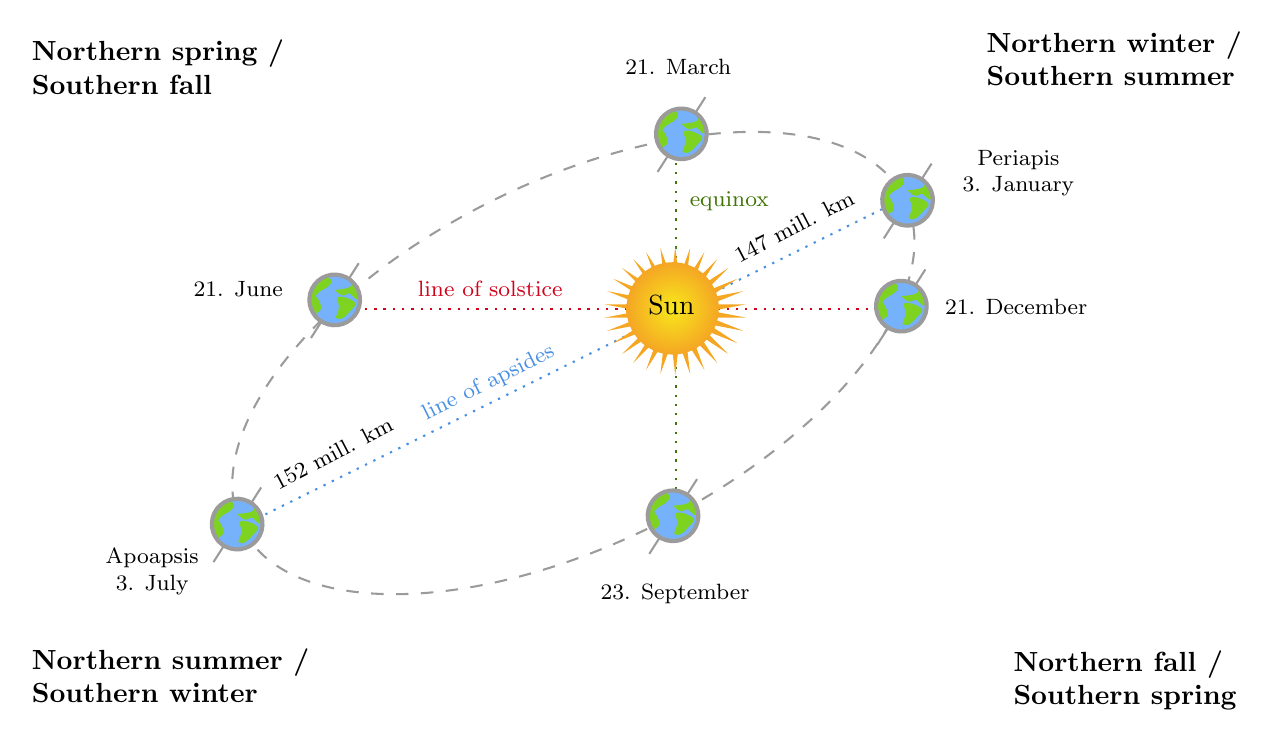
\begin{tikzpicture}[x=0.75pt,y=0.75pt,yscale=-1,xscale=1]
		%uncomment if require: \path (0,916); %set diagram left start at 0, and has height of 916
		
		% Gradient Info		  
		\tikzset {_y515np0jj/.code = {\pgfsetadditionalshadetransform{ \pgftransformshift{\pgfpoint{0 bp } { 0 bp }  }  \pgftransformscale{1 }  }}}
		\pgfdeclareradialshading{_oecpmdnjn}{\pgfpoint{0bp}{0bp}}{rgb(0bp)=(0.97,0.91,0.11);
		rgb(0bp)=(0.97,0.91,0.11);
		rgb(25bp)=(0.96,0.65,0.14);
		rgb(400bp)=(0.96,0.65,0.14)}
		
		%Straight Lines [id:da11453847396278194] 
		\draw [color={rgb, 255:red, 65; green, 117; blue, 5 }  ,draw opacity=1 ] [dash pattern={on 0.84pt off 2.51pt}]  (359,281) -- (359,107) ;
		%Straight Lines [id:da5913309993312645] 
		\draw [color={rgb, 255:red, 208; green, 2; blue, 27 }  ,draw opacity=1 ] [dash pattern={on 0.84pt off 2.51pt}]  (209,185) -- (454,185) ;
		%Straight Lines [id:da8578630699132197] 
		\draw [color={rgb, 255:red, 74; green, 144; blue, 226 }  ,draw opacity=1 ] [dash pattern={on 0.84pt off 2.51pt}]  (161,284) -- (458,137) ;
		%Shape: Star [id:dp2076386297636228] 
		\draw  [draw opacity=0][fill={rgb, 255:red, 245; green, 166; blue, 35 }  ,fill opacity=1 ] (358.5,155) -- (360.3,170.58) -- (365.67,155.68) -- (363.83,171.26) -- (372.53,157.68) -- (367.13,172.58) -- (378.78,160.92) -- (370.04,174.48) -- (384.14,165.26) -- (372.46,176.89) -- (388.38,170.5) -- (374.26,179.7) -- (391.31,176.42) -- (375.37,182.78) -- (392.81,182.76) -- (375.75,186) -- (392.81,189.24) -- (375.37,189.22) -- (391.31,195.58) -- (374.26,192.3) -- (388.38,201.5) -- (372.46,195.11) -- (384.14,206.74) -- (370.04,197.52) -- (378.78,211.08) -- (367.13,199.42) -- (372.53,214.32) -- (363.83,200.74) -- (365.67,216.32) -- (360.3,201.42) -- (358.5,217) -- (356.7,201.42) -- (351.33,216.32) -- (353.17,200.74) -- (344.47,214.32) -- (349.88,199.42) -- (338.22,211.08) -- (346.96,197.52) -- (332.86,206.74) -- (344.54,195.11) -- (328.62,201.5) -- (342.74,192.3) -- (325.69,195.58) -- (341.63,189.22) -- (324.19,189.24) -- (341.25,186) -- (324.19,182.76) -- (341.63,182.78) -- (325.69,176.42) -- (342.74,179.7) -- (328.62,170.5) -- (344.54,176.89) -- (332.86,165.26) -- (346.96,174.48) -- (338.22,160.92) -- (349.88,172.58) -- (344.47,157.68) -- (353.17,171.26) -- (351.33,155.68) -- (356.7,170.58) -- cycle ;
		%Shape: Circle [id:dp5724433743250728] 
		\draw  [draw opacity=0][shading=_oecpmdnjn,_y515np0jj] (335,184.75) .. controls (335,172.46) and (344.96,162.5) .. (357.25,162.5) .. controls (369.54,162.5) and (379.5,172.46) .. (379.5,184.75) .. controls (379.5,197.04) and (369.54,207) .. (357.25,207) .. controls (344.96,207) and (335,197.04) .. (335,184.75) -- cycle ;
		%Shape: Ellipse [id:dp7761703795660999] 
		\draw  [color={rgb, 255:red, 155; green, 155; blue, 155 }  ,draw opacity=1 ][dash pattern={on 4.5pt off 4.5pt}] (149.76,290.29) .. controls (128.31,247.06) and (182.39,176.54) .. (270.56,132.79) .. controls (358.73,89.05) and (447.6,88.63) .. (469.05,131.87) .. controls (490.5,175.1) and (436.42,245.62) .. (348.25,289.37) .. controls (260.08,333.11) and (171.21,333.53) .. (149.76,290.29) -- cycle ;
		%Straight Lines [id:da9587265372771794] 
		\draw [color={rgb, 255:red, 155; green, 155; blue, 155 }  ,draw opacity=1 ]   (350,119) -- (373,83) ;
		%Shape: Ellipse [id:dp6498325616994978] 
		\draw  [draw opacity=0][fill={rgb, 255:red, 118; green, 177; blue, 251 }  ,fill opacity=1 ] (349.72,97.49) .. controls (351.47,91.03) and (358.13,87.2) .. (364.59,88.95) .. controls (371.06,90.7) and (374.88,97.36) .. (373.13,103.82) .. controls (371.38,110.29) and (364.73,114.11) .. (358.26,112.36) .. controls (351.8,110.61) and (347.97,103.95) .. (349.72,97.49) -- cycle ;
		%Shape: Polygon Curved [id:ds5859716383152787] 
		\draw  [draw opacity=0][fill={rgb, 255:red, 126; green, 211; blue, 33 }  ,fill opacity=1 ] (362.72,100.98) .. controls (360.42,96.58) and (373.31,100.85) .. (371.43,103.32) .. controls (369.55,105.79) and (369.03,106.27) .. (366.73,108.36) .. controls (364.42,110.44) and (363.11,109.9) .. (362.08,109.43) .. controls (361.05,108.95) and (365.02,105.38) .. (362.72,100.98) -- cycle ;
		%Shape: Polygon Curved [id:ds4434389182651972] 
		\draw  [draw opacity=0][fill={rgb, 255:red, 126; green, 211; blue, 33 }  ,fill opacity=1 ] (354.46,90.71) .. controls (358.32,87.88) and (361.1,90.69) .. (359.22,93.16) .. controls (357.34,95.63) and (354.37,95.72) .. (352.87,98.03) .. controls (351.37,100.33) and (350.53,99.52) .. (349.86,98.76) .. controls (349.2,98) and (350.6,93.54) .. (354.46,90.71) -- cycle ;
		%Shape: Polygon Curved [id:ds09108101615569808] 
		\draw  [draw opacity=0][fill={rgb, 255:red, 126; green, 211; blue, 33 }  ,fill opacity=1 ] (349.53,98.19) .. controls (350.17,94.78) and (356.4,103.07) .. (354.52,105.54) .. controls (352.64,108.01) and (353.68,105.41) .. (352.65,107.07) .. controls (351.62,108.72) and (351.15,107.24) .. (350.34,105.57) .. controls (349.54,103.9) and (348.9,101.6) .. (349.53,98.19) -- cycle ;
		%Shape: Polygon Curved [id:ds23725716509388461] 
		\draw  [draw opacity=0][fill={rgb, 255:red, 126; green, 211; blue, 33 }  ,fill opacity=1 ] (369.57,92.48) .. controls (367.98,89.05) and (374.89,97.32) .. (373.01,99.8) .. controls (371.13,102.27) and (369.53,95.85) .. (367.22,97.94) .. controls (364.91,100.03) and (362.49,96.47) .. (361.46,95.99) .. controls (360.42,95.52) and (371.16,95.91) .. (369.57,92.48) -- cycle ;
		%Shape: Ellipse [id:dp6232039576419321] 
		\draw  [color={rgb, 255:red, 155; green, 155; blue, 155 }  ,draw opacity=1 ][line width=1.5]  (349.65,97.47) .. controls (351.41,90.96) and (358.11,87.12) .. (364.61,88.88) .. controls (371.12,90.64) and (374.97,97.34) .. (373.21,103.84) .. controls (371.45,110.35) and (364.75,114.2) .. (358.24,112.44) .. controls (351.74,110.68) and (347.89,103.97) .. (349.65,97.47) -- cycle ;
		
		
		%Straight Lines [id:da5118750675334329] 
		\draw [color={rgb, 255:red, 155; green, 155; blue, 155 }  ,draw opacity=1 ]   (459,151) -- (482,115) ;
		%Shape: Ellipse [id:dp9125138855806585] 
		\draw  [draw opacity=0][fill={rgb, 255:red, 118; green, 177; blue, 251 }  ,fill opacity=1 ] (458.72,129.49) .. controls (460.47,123.03) and (467.13,119.2) .. (473.59,120.95) .. controls (480.06,122.7) and (483.88,129.36) .. (482.13,135.82) .. controls (480.38,142.29) and (473.73,146.11) .. (467.26,144.36) .. controls (460.8,142.61) and (456.97,135.95) .. (458.72,129.49) -- cycle ;
		%Shape: Polygon Curved [id:ds9446429261104934] 
		\draw  [draw opacity=0][fill={rgb, 255:red, 126; green, 211; blue, 33 }  ,fill opacity=1 ] (471.72,132.98) .. controls (469.42,128.58) and (482.31,132.85) .. (480.43,135.32) .. controls (478.55,137.79) and (478.03,138.27) .. (475.73,140.36) .. controls (473.42,142.44) and (472.11,141.9) .. (471.08,141.43) .. controls (470.05,140.95) and (474.02,137.38) .. (471.72,132.98) -- cycle ;
		%Shape: Polygon Curved [id:ds567889754281466] 
		\draw  [draw opacity=0][fill={rgb, 255:red, 126; green, 211; blue, 33 }  ,fill opacity=1 ] (463.46,122.71) .. controls (467.32,119.88) and (470.1,122.69) .. (468.22,125.16) .. controls (466.34,127.63) and (463.37,127.72) .. (461.87,130.03) .. controls (460.37,132.33) and (459.53,131.52) .. (458.86,130.76) .. controls (458.2,130) and (459.6,125.54) .. (463.46,122.71) -- cycle ;
		%Shape: Polygon Curved [id:ds07349699102205332] 
		\draw  [draw opacity=0][fill={rgb, 255:red, 126; green, 211; blue, 33 }  ,fill opacity=1 ] (458.53,130.19) .. controls (459.17,126.78) and (465.4,135.07) .. (463.52,137.54) .. controls (461.64,140.01) and (462.68,137.41) .. (461.65,139.07) .. controls (460.62,140.72) and (460.15,139.24) .. (459.34,137.57) .. controls (458.54,135.9) and (457.9,133.6) .. (458.53,130.19) -- cycle ;
		%Shape: Polygon Curved [id:ds9040886632930158] 
		\draw  [draw opacity=0][fill={rgb, 255:red, 126; green, 211; blue, 33 }  ,fill opacity=1 ] (478.57,124.48) .. controls (476.98,121.05) and (483.89,129.32) .. (482.01,131.8) .. controls (480.13,134.27) and (478.53,127.85) .. (476.22,129.94) .. controls (473.91,132.03) and (471.49,128.47) .. (470.46,127.99) .. controls (469.42,127.52) and (480.16,127.91) .. (478.57,124.48) -- cycle ;
		%Shape: Ellipse [id:dp0015009593931776255] 
		\draw  [color={rgb, 255:red, 155; green, 155; blue, 155 }  ,draw opacity=1 ][line width=1.5]  (458.65,129.47) .. controls (460.41,122.96) and (467.11,119.12) .. (473.61,120.88) .. controls (480.12,122.64) and (483.97,129.34) .. (482.21,135.84) .. controls (480.45,142.35) and (473.75,146.2) .. (467.24,144.44) .. controls (460.74,142.68) and (456.89,135.97) .. (458.65,129.47) -- cycle ;
		
		
		%Straight Lines [id:da9838091785436405] 
		\draw [color={rgb, 255:red, 155; green, 155; blue, 155 }  ,draw opacity=1 ]   (456,202) -- (479,166) ;
		%Shape: Ellipse [id:dp04214851236938699] 
		\draw  [draw opacity=0][fill={rgb, 255:red, 118; green, 177; blue, 251 }  ,fill opacity=1 ] (455.72,180.49) .. controls (457.47,174.03) and (464.13,170.2) .. (470.59,171.95) .. controls (477.06,173.7) and (480.88,180.36) .. (479.13,186.82) .. controls (477.38,193.29) and (470.73,197.11) .. (464.26,195.36) .. controls (457.8,193.61) and (453.97,186.95) .. (455.72,180.49) -- cycle ;
		%Shape: Polygon Curved [id:ds5049743817751202] 
		\draw  [draw opacity=0][fill={rgb, 255:red, 126; green, 211; blue, 33 }  ,fill opacity=1 ] (468.72,183.98) .. controls (466.42,179.58) and (479.31,183.85) .. (477.43,186.32) .. controls (475.55,188.79) and (475.03,189.27) .. (472.73,191.36) .. controls (470.42,193.44) and (469.11,192.9) .. (468.08,192.43) .. controls (467.05,191.95) and (471.02,188.38) .. (468.72,183.98) -- cycle ;
		%Shape: Polygon Curved [id:ds5807101871561653] 
		\draw  [draw opacity=0][fill={rgb, 255:red, 126; green, 211; blue, 33 }  ,fill opacity=1 ] (460.46,173.71) .. controls (464.32,170.88) and (467.1,173.69) .. (465.22,176.16) .. controls (463.34,178.63) and (460.37,178.72) .. (458.87,181.03) .. controls (457.37,183.33) and (456.53,182.52) .. (455.86,181.76) .. controls (455.2,181) and (456.6,176.54) .. (460.46,173.71) -- cycle ;
		%Shape: Polygon Curved [id:ds08667612256077928] 
		\draw  [draw opacity=0][fill={rgb, 255:red, 126; green, 211; blue, 33 }  ,fill opacity=1 ] (455.53,181.19) .. controls (456.17,177.78) and (462.4,186.07) .. (460.52,188.54) .. controls (458.64,191.01) and (459.68,188.41) .. (458.65,190.07) .. controls (457.62,191.72) and (457.15,190.24) .. (456.34,188.57) .. controls (455.54,186.9) and (454.9,184.6) .. (455.53,181.19) -- cycle ;
		%Shape: Polygon Curved [id:ds3803948033469786] 
		\draw  [draw opacity=0][fill={rgb, 255:red, 126; green, 211; blue, 33 }  ,fill opacity=1 ] (475.57,175.48) .. controls (473.98,172.05) and (480.89,180.32) .. (479.01,182.8) .. controls (477.13,185.27) and (475.53,178.85) .. (473.22,180.94) .. controls (470.91,183.03) and (468.49,179.47) .. (467.46,178.99) .. controls (466.42,178.52) and (477.16,178.91) .. (475.57,175.48) -- cycle ;
		%Shape: Ellipse [id:dp507541056140181] 
		\draw  [color={rgb, 255:red, 155; green, 155; blue, 155 }  ,draw opacity=1 ][line width=1.5]  (455.65,180.47) .. controls (457.41,173.96) and (464.11,170.12) .. (470.61,171.88) .. controls (477.12,173.64) and (480.97,180.34) .. (479.21,186.84) .. controls (477.45,193.35) and (470.75,197.2) .. (464.24,195.44) .. controls (457.74,193.68) and (453.89,186.97) .. (455.65,180.47) -- cycle ;
		
		
		%Straight Lines [id:da8931764210591124] 
		\draw [color={rgb, 255:red, 155; green, 155; blue, 155 }  ,draw opacity=1 ]   (346,303) -- (369,267) ;
		%Shape: Ellipse [id:dp9572571541043224] 
		\draw  [draw opacity=0][fill={rgb, 255:red, 118; green, 177; blue, 251 }  ,fill opacity=1 ] (345.72,281.49) .. controls (347.47,275.03) and (354.13,271.2) .. (360.59,272.95) .. controls (367.06,274.7) and (370.88,281.36) .. (369.13,287.82) .. controls (367.38,294.29) and (360.73,298.11) .. (354.26,296.36) .. controls (347.8,294.61) and (343.97,287.95) .. (345.72,281.49) -- cycle ;
		%Shape: Polygon Curved [id:ds8604661513782379] 
		\draw  [draw opacity=0][fill={rgb, 255:red, 126; green, 211; blue, 33 }  ,fill opacity=1 ] (358.72,284.98) .. controls (356.42,280.58) and (369.31,284.85) .. (367.43,287.32) .. controls (365.55,289.79) and (365.03,290.27) .. (362.73,292.36) .. controls (360.42,294.44) and (359.11,293.9) .. (358.08,293.43) .. controls (357.05,292.95) and (361.02,289.38) .. (358.72,284.98) -- cycle ;
		%Shape: Polygon Curved [id:ds6430692141465781] 
		\draw  [draw opacity=0][fill={rgb, 255:red, 126; green, 211; blue, 33 }  ,fill opacity=1 ] (350.46,274.71) .. controls (354.32,271.88) and (357.1,274.69) .. (355.22,277.16) .. controls (353.34,279.63) and (350.37,279.72) .. (348.87,282.03) .. controls (347.37,284.33) and (346.53,283.52) .. (345.86,282.76) .. controls (345.2,282) and (346.6,277.54) .. (350.46,274.71) -- cycle ;
		%Shape: Polygon Curved [id:ds9642854399225493] 
		\draw  [draw opacity=0][fill={rgb, 255:red, 126; green, 211; blue, 33 }  ,fill opacity=1 ] (345.53,282.19) .. controls (346.17,278.78) and (352.4,287.07) .. (350.52,289.54) .. controls (348.64,292.01) and (349.68,289.41) .. (348.65,291.07) .. controls (347.62,292.72) and (347.15,291.24) .. (346.34,289.57) .. controls (345.54,287.9) and (344.9,285.6) .. (345.53,282.19) -- cycle ;
		%Shape: Polygon Curved [id:ds355190996354644] 
		\draw  [draw opacity=0][fill={rgb, 255:red, 126; green, 211; blue, 33 }  ,fill opacity=1 ] (365.57,276.48) .. controls (363.98,273.05) and (370.89,281.32) .. (369.01,283.8) .. controls (367.13,286.27) and (365.53,279.85) .. (363.22,281.94) .. controls (360.91,284.03) and (358.49,280.47) .. (357.46,279.99) .. controls (356.42,279.52) and (367.16,279.91) .. (365.57,276.48) -- cycle ;
		%Shape: Ellipse [id:dp40624723387215456] 
		\draw  [color={rgb, 255:red, 155; green, 155; blue, 155 }  ,draw opacity=1 ][line width=1.5]  (345.65,281.47) .. controls (347.41,274.96) and (354.11,271.12) .. (360.61,272.88) .. controls (367.12,274.64) and (370.97,281.34) .. (369.21,287.84) .. controls (367.45,294.35) and (360.75,298.2) .. (354.24,296.44) .. controls (347.74,294.68) and (343.89,287.97) .. (345.65,281.47) -- cycle ;
		
		
		%Straight Lines [id:da9951910387391516] 
		\draw [color={rgb, 255:red, 155; green, 155; blue, 155 }  ,draw opacity=1 ]   (136,307) -- (159,271) ;
		%Shape: Ellipse [id:dp5574616244328321] 
		\draw  [draw opacity=0][fill={rgb, 255:red, 118; green, 177; blue, 251 }  ,fill opacity=1 ] (135.72,285.49) .. controls (137.47,279.03) and (144.13,275.2) .. (150.59,276.95) .. controls (157.06,278.7) and (160.88,285.36) .. (159.13,291.82) .. controls (157.38,298.29) and (150.73,302.11) .. (144.26,300.36) .. controls (137.8,298.61) and (133.97,291.95) .. (135.72,285.49) -- cycle ;
		%Shape: Polygon Curved [id:ds008787627390895336] 
		\draw  [draw opacity=0][fill={rgb, 255:red, 126; green, 211; blue, 33 }  ,fill opacity=1 ] (148.72,288.98) .. controls (146.42,284.58) and (159.31,288.85) .. (157.43,291.32) .. controls (155.55,293.79) and (155.03,294.27) .. (152.73,296.36) .. controls (150.42,298.44) and (149.11,297.9) .. (148.08,297.43) .. controls (147.05,296.95) and (151.02,293.38) .. (148.72,288.98) -- cycle ;
		%Shape: Polygon Curved [id:ds8244698492819325] 
		\draw  [draw opacity=0][fill={rgb, 255:red, 126; green, 211; blue, 33 }  ,fill opacity=1 ] (140.46,278.71) .. controls (144.32,275.88) and (147.1,278.69) .. (145.22,281.16) .. controls (143.34,283.63) and (140.37,283.72) .. (138.87,286.03) .. controls (137.37,288.33) and (136.53,287.52) .. (135.86,286.76) .. controls (135.2,286) and (136.6,281.54) .. (140.46,278.71) -- cycle ;
		%Shape: Polygon Curved [id:ds4005813261674447] 
		\draw  [draw opacity=0][fill={rgb, 255:red, 126; green, 211; blue, 33 }  ,fill opacity=1 ] (135.53,286.19) .. controls (136.17,282.78) and (142.4,291.07) .. (140.52,293.54) .. controls (138.64,296.01) and (139.68,293.41) .. (138.65,295.07) .. controls (137.62,296.72) and (137.15,295.24) .. (136.34,293.57) .. controls (135.54,291.9) and (134.9,289.6) .. (135.53,286.19) -- cycle ;
		%Shape: Polygon Curved [id:ds9442138989185305] 
		\draw  [draw opacity=0][fill={rgb, 255:red, 126; green, 211; blue, 33 }  ,fill opacity=1 ] (155.57,280.48) .. controls (153.98,277.05) and (160.89,285.32) .. (159.01,287.8) .. controls (157.13,290.27) and (155.53,283.85) .. (153.22,285.94) .. controls (150.91,288.03) and (148.49,284.47) .. (147.46,283.99) .. controls (146.42,283.52) and (157.16,283.91) .. (155.57,280.48) -- cycle ;
		%Shape: Ellipse [id:dp09425646768981255] 
		\draw  [color={rgb, 255:red, 155; green, 155; blue, 155 }  ,draw opacity=1 ][line width=1.5]  (135.65,285.47) .. controls (137.41,278.96) and (144.11,275.12) .. (150.61,276.88) .. controls (157.12,278.64) and (160.97,285.34) .. (159.21,291.84) .. controls (157.45,298.35) and (150.75,302.2) .. (144.24,300.44) .. controls (137.74,298.68) and (133.89,291.97) .. (135.65,285.47) -- cycle ;
		
		
		%Straight Lines [id:da5799013581197077] 
		\draw [color={rgb, 255:red, 155; green, 155; blue, 155 }  ,draw opacity=1 ]   (183,199) -- (206,163) ;
		%Shape: Ellipse [id:dp17453308650730293] 
		\draw  [draw opacity=0][fill={rgb, 255:red, 118; green, 177; blue, 251 }  ,fill opacity=1 ] (182.72,177.49) .. controls (184.47,171.03) and (191.13,167.2) .. (197.59,168.95) .. controls (204.06,170.7) and (207.88,177.36) .. (206.13,183.82) .. controls (204.38,190.29) and (197.73,194.11) .. (191.26,192.36) .. controls (184.8,190.61) and (180.97,183.95) .. (182.72,177.49) -- cycle ;
		%Shape: Polygon Curved [id:ds8090729704788711] 
		\draw  [draw opacity=0][fill={rgb, 255:red, 126; green, 211; blue, 33 }  ,fill opacity=1 ] (195.72,180.98) .. controls (193.42,176.58) and (206.31,180.85) .. (204.43,183.32) .. controls (202.55,185.79) and (202.03,186.27) .. (199.73,188.36) .. controls (197.42,190.44) and (196.11,189.9) .. (195.08,189.43) .. controls (194.05,188.95) and (198.02,185.38) .. (195.72,180.98) -- cycle ;
		%Shape: Polygon Curved [id:ds37621015496263754] 
		\draw  [draw opacity=0][fill={rgb, 255:red, 126; green, 211; blue, 33 }  ,fill opacity=1 ] (187.46,170.71) .. controls (191.32,167.88) and (194.1,170.69) .. (192.22,173.16) .. controls (190.34,175.63) and (187.37,175.72) .. (185.87,178.03) .. controls (184.37,180.33) and (183.53,179.52) .. (182.86,178.76) .. controls (182.2,178) and (183.6,173.54) .. (187.46,170.71) -- cycle ;
		%Shape: Polygon Curved [id:ds7794005166919475] 
		\draw  [draw opacity=0][fill={rgb, 255:red, 126; green, 211; blue, 33 }  ,fill opacity=1 ] (182.53,178.19) .. controls (183.17,174.78) and (189.4,183.07) .. (187.52,185.54) .. controls (185.64,188.01) and (186.68,185.41) .. (185.65,187.07) .. controls (184.62,188.72) and (184.15,187.24) .. (183.34,185.57) .. controls (182.54,183.9) and (181.9,181.6) .. (182.53,178.19) -- cycle ;
		%Shape: Polygon Curved [id:ds5008859820441549] 
		\draw  [draw opacity=0][fill={rgb, 255:red, 126; green, 211; blue, 33 }  ,fill opacity=1 ] (202.57,172.48) .. controls (200.98,169.05) and (207.89,177.32) .. (206.01,179.8) .. controls (204.13,182.27) and (202.53,175.85) .. (200.22,177.94) .. controls (197.91,180.03) and (195.49,176.47) .. (194.46,175.99) .. controls (193.42,175.52) and (204.16,175.91) .. (202.57,172.48) -- cycle ;
		%Shape: Ellipse [id:dp12109855969295191] 
		\draw  [color={rgb, 255:red, 155; green, 155; blue, 155 }  ,draw opacity=1 ][line width=1.5]  (182.65,177.47) .. controls (184.41,170.96) and (191.11,167.12) .. (197.61,168.88) .. controls (204.12,170.64) and (207.97,177.34) .. (206.21,183.84) .. controls (204.45,190.35) and (197.75,194.2) .. (191.24,192.44) .. controls (184.74,190.68) and (180.89,183.97) .. (182.65,177.47) -- cycle ;
		
		
		
		% Text Node
		\draw (344,177) node [anchor=north west][inner sep=0.75pt]   [align=left] {Sun};
		% Text Node
		\draw (487,179) node [anchor=north west][inner sep=0.75pt]  [font=\footnotesize] [align=left] {21. December};
		% Text Node
		\draw (321,316) node [anchor=north west][inner sep=0.75pt]  [font=\footnotesize] [align=left] {23. September};
		% Text Node
		\draw (333,63) node [anchor=north west][inner sep=0.75pt]  [font=\footnotesize] [align=left] {21. March};
		% Text Node
		\draw (125,170) node [anchor=north west][inner sep=0.75pt]  [font=\footnotesize] [align=left] {21. June};
		% Text Node
		\draw (489,107) node [anchor=north west][inner sep=0.75pt]  [font=\footnotesize] [align=left] {\begin{minipage}[lt]{50pt}\setlength\topsep{0pt}
		\begin{center}
		Periapis\\3. January
		\end{center}
		
		\end{minipage}};
		% Text Node
		\draw (75,299) node [anchor=north west][inner sep=0.75pt]  [font=\footnotesize] [align=left] {\begin{minipage}[lt]{45pt}\setlength\topsep{0pt}
		\begin{center}
		Apoapsis\\3. July
		\end{center}
		
		\end{minipage}};
		% Text Node
		\draw (47,54) node [anchor=north west][inner sep=0.75pt]   [align=left] {\textbf{Northern spring / }\\\textbf{Southern fall}};
		% Text Node
		\draw (47,347) node [anchor=north west][inner sep=0.75pt]   [align=left] {\textbf{Northern summer / }\\\textbf{Southern winter}};
		% Text Node
		\draw (520,348) node [anchor=north west][inner sep=0.75pt]   [align=left] {\textbf{Northern fall / }\\\textbf{Southern spring}};
		% Text Node
		\draw (507,50) node [anchor=north west][inner sep=0.75pt]   [align=left] {\textbf{Northern winter / }\\\textbf{Southern summer}};
		% Text Node
		\draw (364,127) node [anchor=north west][inner sep=0.75pt]  [font=\footnotesize] [align=left] {\textcolor[rgb]{0.25,0.46,0.02}{equinox}};
		% Text Node
		\draw (233,170) node [anchor=north west][inner sep=0.75pt]  [font=\footnotesize] [align=left] {\textcolor[rgb]{0.82,0.01,0.11}{line of solstice}};
		% Text Node
		\draw (233.25,231.3) node [anchor=north west][inner sep=0.75pt]  [font=\footnotesize,color={rgb, 255:red, 74; green, 144; blue, 226 }  ,opacity=1 ,rotate=-333.51] [align=left] {\textcolor[rgb]{0.29,0.56,0.89}{line of apsides}};
		% Text Node
		\draw (161.8,265.18) node [anchor=north west][inner sep=0.75pt]  [rotate=-332.53] [align=left] {{\footnotesize $\displaystyle 152$ mill. km}};
		% Text Node
		\draw (384,156) node [anchor=north west][inner sep=0.75pt]  [rotate=-332.53] [align=left] {{\footnotesize $\displaystyle 147$ mill. km}};
		
		\end{tikzpicture}
		\vspace*{3mm}	
		\caption{Representation of the rotation of the Earth on its orbit with its major phases}
	\end{figure}
	\begin{tcolorbox}[title=Remark,arc=10pt,breakable,drop lifted shadow,
  skin=enhanced,
  skin first is subskin of={enhancedfirst}{arc=10pt,no shadow},
  skin middle is subskin of={enhancedmiddle}{arc=10pt,no shadow},
  skin last is subskin of={enhancedlast}{drop lifted shadow}]
	It is obvious that, given the complexity of the problem, we will simplify it by considering a circular orbit without variations (precession, nutation) of the axis of rotation of the Earth. We will assume that the Sun is reduced to a point (no dawn or twilight, etc.).
	\end{tcolorbox}
	Let us first recall that the precession is the gradual change in direction of the axis of rotation of an object when a torque (force) is applied to it while the nutation is a periodic balancing of the axis of rotation of the Earth around its mean position in addition to the precession (\SeeChapter{see section Classical Mechanics page \pageref{gyroscope}}).
	\begin{figure}[H]
		\centering
		\includegraphics{img/cosmology/nutation_precession_earth.jpg}
	\end{figure}
	Let us represent the Earth with its vertical axis of rotation. Accordingly the equator will be located in a horizontal plane.

	Suppose that day, the Earth is in such a position that the Sun's rays form an angle $\alpha$ with the equatorial plane (or conversely that the axis of the Earth form an angle with the equatorial plane). Notice that this angle $\alpha$ will always be according to actual measurements  between $-23^\circ 27'$ and $+23^\circ 27'$ at least... at a human life time scale...
	
	For our example we have chosen to focus our analysis on a day when $\alpha$ is positive. Thus, in the northern hemisphere, we are close to the summer solstice!

	We are looking for the day length at a place located at latitude $\lambda$! To fix ideas, we place ourselves around Brussels at $50^\circ$ north latitude.
	
	Let us now consider the following figures where the first is a view of the side of Earth at a time $t$ of its orbit when $\alpha>0$ and the second in to a cylindrical cutting of diameter $\overline{NJ}$ (corresponding to the diameter of the parallel of Brussels) of Earth's volume Earth at this same moment:
	\begin{figure}[H]
		\centering
		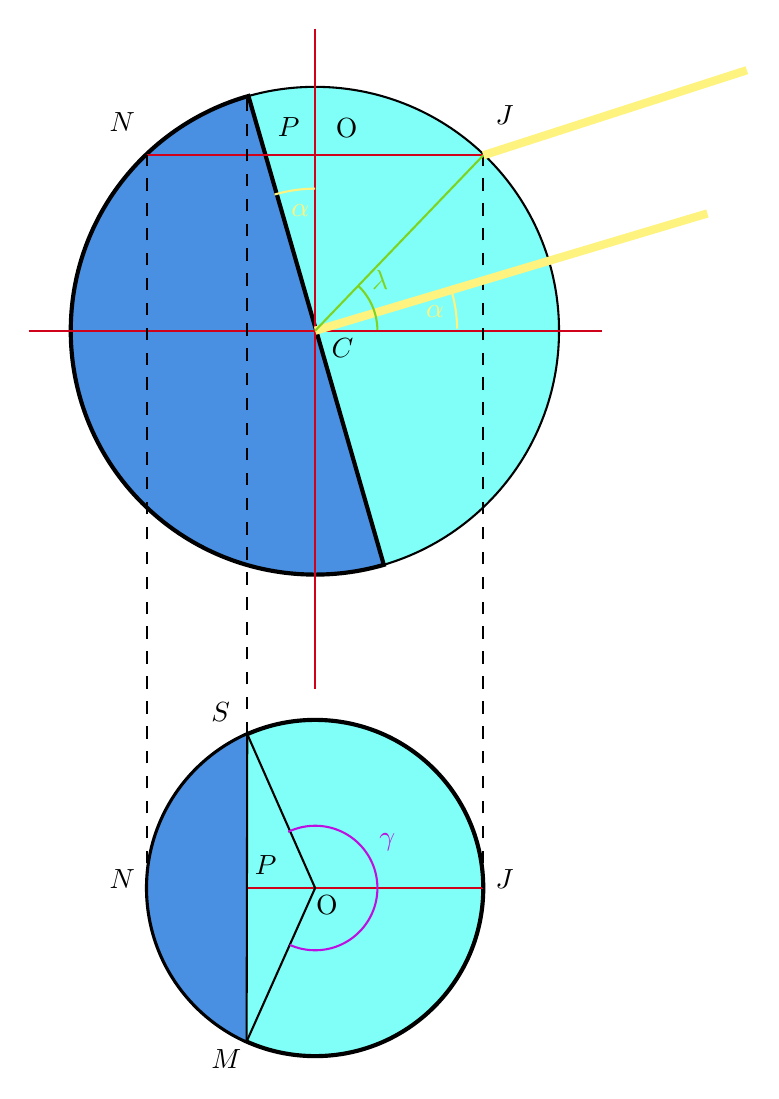
\begin{tikzpicture}[x=0.75pt,y=0.75pt,yscale=-1,xscale=1]
		%uncomment if require: \path (0,1215); %set diagram left start at 0, and has height of 1215
		
		%Shape: Circle [id:dp09933114152492939] 
		\draw  [fill={rgb, 255:red, 127; green, 255; blue, 248 }  ,fill opacity=1 ] (215,191.5) .. controls (215,126.61) and (267.61,74) .. (332.5,74) .. controls (397.39,74) and (450,126.61) .. (450,191.5) .. controls (450,256.39) and (397.39,309) .. (332.5,309) .. controls (267.61,309) and (215,256.39) .. (215,191.5) -- cycle ;
		%Shape: Circle [id:dp41313355817955255] 
		\draw  [fill={rgb, 255:red, 127; green, 255; blue, 248 }  ,fill opacity=1 ][line width=1.5]  (251.5,460) .. controls (251.5,415.26) and (287.76,379) .. (332.5,379) .. controls (377.24,379) and (413.5,415.26) .. (413.5,460) .. controls (413.5,504.74) and (377.24,541) .. (332.5,541) .. controls (287.76,541) and (251.5,504.74) .. (251.5,460) -- cycle ;
		%Straight Lines [id:da3674205180982708] 
		\draw [color={rgb, 255:red, 208; green, 2; blue, 27 }  ,draw opacity=1 ]   (251.5,460) -- (413.5,460) ;
		%Shape: Chord [id:dp3713365316533548] 
		\draw  [fill={rgb, 255:red, 74; green, 144; blue, 226 }  ,fill opacity=1 ] (299.48,533.99) .. controls (271.2,521.35) and (251.5,492.98) .. (251.5,460) .. controls (251.5,426.9) and (271.35,398.44) .. (299.79,385.87) -- cycle ;
		%Shape: Chord [id:dp28594922506274023] 
		\draw  [fill={rgb, 255:red, 74; green, 144; blue, 226 }  ,fill opacity=1 ][line width=1.5]  (365.59,304.3) .. controls (355.09,307.36) and (343.99,309) .. (332.5,309) .. controls (267.47,309) and (214.75,256.39) .. (214.75,191.5) .. controls (214.75,137.73) and (250.95,92.39) .. (300.36,78.43) -- cycle ;
		%Straight Lines [id:da19124977115019348] 
		\draw [color={rgb, 255:red, 208; green, 2; blue, 27 }  ,draw opacity=1 ]   (251.5,107) -- (413.5,107) ;
		%Straight Lines [id:da31166800536085737] 
		\draw [color={rgb, 255:red, 208; green, 2; blue, 27 }  ,draw opacity=1 ]   (332.5,46) -- (332.5,364) ;
		%Straight Lines [id:da8599868312979615] 
		\draw [color={rgb, 255:red, 208; green, 2; blue, 27 }  ,draw opacity=1 ]   (194.5,191.5) -- (470.5,191.5) ;
		%Straight Lines [id:da6855745064350334] 
		\draw  [dash pattern={on 4.5pt off 4.5pt}]  (299.79,385.87) -- (299.79,78.6) ;
		%Straight Lines [id:da13013496025251658] 
		\draw  [dash pattern={on 4.5pt off 4.5pt}]  (251.5,460) -- (251.5,107) ;
		%Straight Lines [id:da8361902703526771] 
		\draw  [dash pattern={on 4.5pt off 4.5pt}]  (413.5,460) -- (413.5,107) ;
		%Straight Lines [id:da7096360992269859] 
		\draw    (299.79,385.87) -- (332.5,460) ;
		%Straight Lines [id:da4152954893255074] 
		\draw    (299.48,533.99) -- (332.5,460) ;
		%Straight Lines [id:da410164637341925] 
		\draw [color={rgb, 255:red, 255; green, 243; blue, 128 }  ,draw opacity=1 ][line width=3]    (413.5,107) -- (540.5,66) ;
		%Straight Lines [id:da2428569847246087] 
		\draw [color={rgb, 255:red, 255; green, 243; blue, 128 }  ,draw opacity=1 ][line width=3]    (332.5,191.5) -- (521.5,135) ;
		%Shape: Arc [id:dp008354809259261575] 
		\draw  [draw opacity=0] (319.52,432.95) .. controls (323.44,431.06) and (327.85,430) .. (332.5,430) .. controls (349.07,430) and (362.5,443.43) .. (362.5,460) .. controls (362.5,476.57) and (349.07,490) .. (332.5,490) .. controls (328.16,490) and (324.04,489.08) .. (320.31,487.42) -- (332.5,460) -- cycle ; \draw  [color={rgb, 255:red, 189; green, 16; blue, 224 }  ,draw opacity=1 ] (319.52,432.95) .. controls (323.44,431.06) and (327.85,430) .. (332.5,430) .. controls (349.07,430) and (362.5,443.43) .. (362.5,460) .. controls (362.5,476.57) and (349.07,490) .. (332.5,490) .. controls (328.16,490) and (324.04,489.08) .. (320.31,487.42) ;  
		%Shape: Arc [id:dp33821918546679197] 
		\draw  [draw opacity=0] (353.34,169.92) .. controls (358.89,175.29) and (362.38,182.77) .. (362.5,191.07) -- (332.5,191.5) -- cycle ; \draw  [color={rgb, 255:red, 126; green, 211; blue, 33 }  ,draw opacity=1 ] (353.34,169.92) .. controls (358.89,175.29) and (362.38,182.77) .. (362.5,191.07) ;  
		%Straight Lines [id:da6997967754291308] 
		\draw [color={rgb, 255:red, 126; green, 211; blue, 33 }  ,draw opacity=1 ]   (332.5,191.5) -- (413.5,107) ;
		%Shape: Arc [id:dp7231226867131402] 
		\draw  [draw opacity=0] (398.32,172.69) .. controls (399.94,178.37) and (400.84,184.34) .. (400.93,190.52) -- (332.5,191.5) -- cycle ; \draw  [color={rgb, 255:red, 255; green, 243; blue, 128 }  ,draw opacity=1 ] (398.32,172.69) .. controls (399.94,178.37) and (400.84,184.34) .. (400.93,190.52) ;  
		%Shape: Arc [id:dp9141757572954956] 
		\draw  [draw opacity=0] (312.95,125.89) .. controls (319.15,124.05) and (325.71,123.06) .. (332.5,123.06) -- (332.5,191.5) -- cycle ; \draw  [color={rgb, 255:red, 255; green, 243; blue, 128 }  ,draw opacity=1 ] (312.95,125.89) .. controls (319.15,124.05) and (325.71,123.06) .. (332.5,123.06) ;  
		
		% Text Node
		\draw (232,449.4) node [anchor=north west][inner sep=0.75pt]    {$N$};
		% Text Node
		\draw (281,369.4) node [anchor=north west][inner sep=0.75pt]    {$S$};
		% Text Node
		\draw (281,536.4) node [anchor=north west][inner sep=0.75pt]    {$M$};
		% Text Node
		\draw (302,443) node [anchor=north west][inner sep=0.75pt]    {$P$};
		% Text Node
		\draw (331.5,462) node [anchor=north west][inner sep=0.75pt]   [align=left] {O};
		% Text Node
		\draw (418,449.4) node [anchor=north west][inner sep=0.75pt]    {$J$};
		% Text Node
		\draw (232,85) node [anchor=north west][inner sep=0.75pt]    {$N$};
		% Text Node
		\draw (418,81.4) node [anchor=north west][inner sep=0.75pt]    {$J$};
		% Text Node
		\draw (313,87.4) node [anchor=north west][inner sep=0.75pt]    {$P$};
		% Text Node
		\draw (341,88) node [anchor=north west][inner sep=0.75pt]   [align=left] {O};
		% Text Node
		\draw (339,194) node [anchor=north west][inner sep=0.75pt]    {$C$};
		% Text Node
		\draw (362,432.4) node [anchor=north west][inner sep=0.75pt]  [color={rgb, 255:red, 189; green, 16; blue, 224 }  ,opacity=1 ]  {$\gamma $};
		% Text Node
		\draw (358.5,161) node [anchor=north west][inner sep=0.75pt]  [color={rgb, 255:red, 126; green, 211; blue, 33 }  ,opacity=1 ]  {$\lambda $};
		% Text Node
		\draw (384.5,178) node [anchor=north west][inner sep=0.75pt]  [color={rgb, 255:red, 255; green, 243; blue, 128 }  ,opacity=1 ]  {$\alpha $};
		% Text Node
		\draw (319.5,129) node [anchor=north west][inner sep=0.75pt]  [color={rgb, 255:red, 255; green, 243; blue, 128 }  ,opacity=1 ]  {$\alpha $};
		
		\end{tikzpicture}
	\end{figure}
	In the figure above, $C$ denotes the center of the Earth, and O the center of the parallel of Brussels.

	Let us fix a time $t$ and denote by $M$ (morning) and $S$ (evening) the two points of the parallel of Brussels where the Sun rises and sets (these points will be considered fixed whatever the moment $t$, which is obviously wrong relatively to the reality), while $J$ (day) and $N$ (night) will be the points where it is noon and midnight respectively.

	$P$ will be the point on the disc corresponding to the Brussels parallel where the meridian noon plane  (the plan which of the sides is $\overline{NJ}$) cut the line $\overline{MS}$.

	Finally, $\gamma$ designate the angle $\widehat{M\text{O}S}$ (where O is the center of the disk generated by the parallel of Brussels) behind the illuminated part by the Sun and $r$ designate the radius $S\text{O}=M\text{O}$.

	To simplify the problem, let us also assume... that during $24$ hours the Earth rotates on itself without changing the position of its axis of rotation relative to the Sun....

	The angle $\gamma$ can be calculated by noting that $\overline{\text{O}P}$ is, in absolute value equal to:
	
	where $r$ represents for recall the radius of the parallel of Brussels.
	
	Using the properties of trigonometric functions (\SeeChapter{see section Trigonometry page \pageref{remarkable trigonometric identities}}), we have:
	
	But we still need to inject the parameter $\alpha$. Knowing the latitude $\lambda$ of Brussels, we have:
	
	where $R$ is the radius of the Earth.

	We have also:
	
	and in the triangle $C\text{O}P$:
	
	Finally, by comparing the values obtained for $\overline{P\text{O}}$, we get:
	
	and as:
	
	We finally get:
	
	and therefore:
	
	At the equinoxes (that is to say when the equator coincides with the ecliptic plane for recall...) we have $\alpha=0$ and therefore:
	
	However, as we have specified it at the beginning, we must take the absolute value thus:
	
	In other words, whatever the latitude we take, the angle formed by the night area is equal to the angle formed by the day area at equinoxes (both being equal to $\pi$).

	Let us now consider the summer solstice, when $\alpha=23^\circ 27'$ still considering the latitude of Brussels $\lambda=50^\circ$, we have:
	
	This translated into hours by:
	
	So the 24-hour day loses $7.9$ hours. Which is equivalent to a day light of approximately $16$ hours.
	
	In summary to calculate the duration of a "day", it is enough to know two things: the latitude and the angle at which the Sun falls on the plane of the equator to the chosen date. The value of this angle is well known at the equinoxes (it is $0^\circ$) and to the solstices (it is $+23^\circ 27'$ and $-23^\circ 27'$).

	But what about the other dates?
	
	The answer is quite simple. Let us imagine, sitting on the Sun watching throughout the year towards the center of the Earth.

	During its rotation around the Sun (the binomial centroid in fact), the axis of rotation of the Earth maintains its inclination to the ecliptic. Seen from the Sun, this axis revolve around normal to the plane of the ecliptic and therefore describe a cone whose half apex angle is $23^\circ27'$ (see figure below).

	The angle of attack $\alpha$ of the sunlight on the equator therefore vary according to the date $\delta$ (we associate to the date, the angle $\delta$ travelled by the Earth on its orbit, from its position the spring equinox)

	Therefore, the angle $\alpha$ vary according to the date $\delta$ sinusoidally.

	For those who are perhaps not convinced by this semi-intuitive reasoning, here's another approach:

	For readability of the diagram, we have greatly exaggerated the angle of the axis of rotation of the Earth with the ecliptic (and obviously nothing is to scale...!):
	\begin{figure}[H]
		\centering
		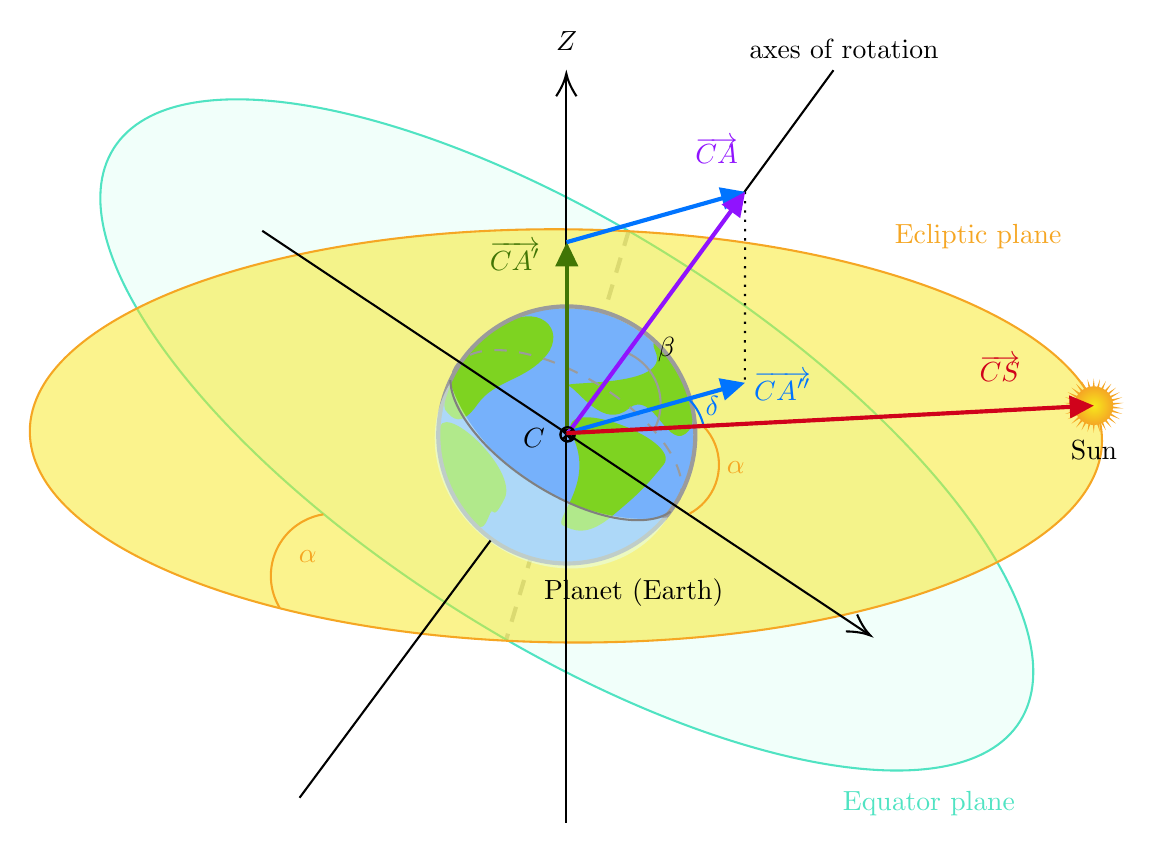
\begin{tikzpicture}[x=0.75pt,y=0.75pt,yscale=-1,xscale=1]
		%uncomment if require: \path (0,1077); %set diagram left start at 0, and has height of 1077
		
		% Gradient Info
		  
		\tikzset {_45fn30b5g/.code = {\pgfsetadditionalshadetransform{ \pgftransformshift{\pgfpoint{0 bp } { 0 bp }  }  \pgftransformscale{1 }  }}}
		\pgfdeclareradialshading{_5xsxpkpbm}{\pgfpoint{0bp}{0bp}}{rgb(0bp)=(0.97,0.91,0.11);
		rgb(0bp)=(0.97,0.91,0.11);
		rgb(25bp)=(0.96,0.65,0.14);
		rgb(400bp)=(0.96,0.65,0.14)}
		
		%Straight Lines [id:da824449054914073] 
		\draw [color={rgb, 255:red, 155; green, 155; blue, 155 }  ,draw opacity=1 ][line width=1.5]  [dash pattern={on 5.63pt off 4.5pt}]  (330.4,229.8) -- (271.2,427.4) ;
		%Shape: Ellipse [id:dp16403351561736557] 
		\draw  [color={rgb, 255:red, 80; green, 227; blue, 194 }  ,draw opacity=1 ][fill={rgb, 255:red, 228; green, 255; blue, 246 }  ,fill opacity=0.5 ] (247.39,412.23) .. controls (126.82,335.99) and (52.9,236.51) .. (82.29,190.05) .. controls (111.67,143.6) and (233.22,167.74) .. (353.79,243.99) .. controls (474.35,320.24) and (548.27,419.71) .. (518.89,466.17) .. controls (489.51,512.63) and (367.95,488.48) .. (247.39,412.23) -- cycle ;
		%Shape: Ellipse [id:dp47717617431481774] 
		\draw  [color={rgb, 255:red, 245; green, 166; blue, 35 }  ,draw opacity=1 ][fill={rgb, 255:red, 248; green, 231; blue, 28 }  ,fill opacity=0.5 ] (299.18,428.1) .. controls (156.54,426.71) and (41.34,381.02) .. (41.87,326.05) .. controls (42.41,271.08) and (158.48,227.66) .. (301.13,229.05) .. controls (443.77,230.44) and (558.97,276.13) .. (558.44,331.1) .. controls (557.9,386.07) and (441.83,429.5) .. (299.18,428.1) -- cycle ;
		%Shape: Circle [id:dp8572843883954031] 
		\draw  [draw opacity=0][fill={rgb, 255:red, 118; green, 177; blue, 251 }  ,fill opacity=1 ] (238.63,328.58) .. controls (238.63,294.6) and (266.18,267.05) .. (300.16,267.05) .. controls (334.13,267.05) and (361.68,294.6) .. (361.68,328.58) .. controls (361.68,362.55) and (334.13,390.1) .. (300.16,390.1) .. controls (266.18,390.1) and (238.63,362.55) .. (238.63,328.58) -- cycle ;
		%Shape: Polygon Curved [id:ds72086251712952] 
		\draw  [draw opacity=0][fill={rgb, 255:red, 126; green, 211; blue, 33 }  ,fill opacity=1 ] (303.49,329.01) .. controls (292.65,306.3) and (357.2,330.25) .. (347.22,342.45) .. controls (337.24,354.65) and (334.53,356.99) .. (322.46,367.14) .. controls (310.38,377.3) and (303.86,374.29) .. (298.71,371.71) .. controls (293.55,369.12) and (314.32,351.72) .. (303.49,329.01) -- cycle ;
		%Shape: Polygon Curved [id:ds002928123545772543] 
		\draw  [draw opacity=0][fill={rgb, 255:red, 126; green, 211; blue, 33 }  ,fill opacity=1 ] (267.08,276.42) .. controls (287.18,262.79) and (300.74,277.51) .. (290.76,289.71) .. controls (280.78,301.9) and (265.68,301.79) .. (257.67,313.22) .. controls (249.67,324.64) and (245.53,320.38) .. (242.29,316.4) .. controls (239.06,312.42) and (246.98,290.05) .. (267.08,276.42) -- cycle ;
		%Shape: Polygon Curved [id:ds8367232596623717] 
		\draw  [draw opacity=0][fill={rgb, 255:red, 126; green, 211; blue, 33 }  ,fill opacity=1 ] (238.97,326.73) .. controls (238.99,309.13) and (277.69,344.76) .. (270.59,358.83) .. controls (263.48,372.9) and (266.3,358.95) .. (262.68,368.17) .. controls (259.07,377.39) and (255.36,370.42) .. (249.8,362.83) .. controls (244.24,355.24) and (238.95,344.34) .. (238.97,326.73) -- cycle ;
		%Shape: Polygon Curved [id:ds1667158585643418] 
		\draw  [draw opacity=0][fill={rgb, 255:red, 126; green, 211; blue, 33 }  ,fill opacity=1 ] (343.37,288.12) .. controls (335.94,270.43) and (369.46,313.67) .. (359.48,325.87) .. controls (349.5,338.07) and (342.54,305.24) .. (330.46,315.4) .. controls (318.38,325.55) and (306.73,307.06) .. (301.58,304.47) .. controls (296.42,301.88) and (350.8,305.81) .. (343.37,288.12) -- cycle ;
		%Shape: Circle [id:dp1020985724130885] 
		\draw  [color={rgb, 255:red, 155; green, 155; blue, 155 }  ,draw opacity=1 ][line width=1.5]  (241.44,309.8) .. controls (251.56,277.14) and (286.23,258.86) .. (318.9,268.97) .. controls (351.56,279.08) and (369.84,313.76) .. (359.73,346.42) .. controls (349.62,379.08) and (314.94,397.37) .. (282.28,387.26) .. controls (249.62,377.14) and (231.33,342.47) .. (241.44,309.8) -- cycle ;
		
		%Flowchart: Summing Junction [id:dp1649397169994682] 
		\draw   (297.55,328.11) .. controls (297.55,326.44) and (298.91,325.08) .. (300.59,325.08) .. controls (302.26,325.08) and (303.62,326.44) .. (303.62,328.11) .. controls (303.62,329.79) and (302.26,331.15) .. (300.59,331.15) .. controls (298.91,331.15) and (297.55,329.79) .. (297.55,328.11) -- cycle ; \draw   (298.44,325.97) -- (302.73,330.26) ; \draw   (302.73,325.97) -- (298.44,330.26) ;
		%Shape: Arc [id:dp11078006012480879] 
		\draw  [draw opacity=0][dash pattern={on 4.5pt off 4.5pt}] (245.75,297.84) .. controls (246.06,297) and (246.45,296.2) .. (246.92,295.43) .. controls (255.26,281.85) and (285.95,285.54) .. (315.47,303.66) .. controls (343.66,320.98) and (360.58,345.22) .. (354.77,359.19) -- (300.36,328.26) -- cycle ; \draw  [color={rgb, 255:red, 155; green, 155; blue, 155 }  ,draw opacity=1 ][dash pattern={on 4.5pt off 4.5pt}] (245.75,297.84) .. controls (246.06,297) and (246.45,296.2) .. (246.92,295.43) .. controls (255.26,281.85) and (285.95,285.54) .. (315.47,303.66) .. controls (343.66,320.98) and (360.58,345.22) .. (354.77,359.19) ;  
		%Shape: Moon [id:dp014934701038201936] 
		\draw  [draw opacity=0][fill={rgb, 255:red, 228; green, 255; blue, 246 }  ,fill opacity=0.5 ][line width=1.5]  (349.2,367.8) .. controls (333.17,393.73) and (296.74,400.25) .. (267.81,382.37) .. controls (238.89,364.5) and (228.43,328.99) .. (244.46,303.06) .. controls (250.34,321.26) and (265.04,339.64) .. (286.16,352.7) .. controls (307.28,365.75) and (330.29,370.68) .. (349.2,367.8) -- cycle ;
		%Shape: Arc [id:dp4835272793326104] 
		\draw  [draw opacity=0] (350.54,365.02) .. controls (338.86,373.75) and (311.3,368.54) .. (284.82,351.74) .. controls (260.56,336.34) and (244.72,315.98) .. (244.49,301.68) -- (300.36,327.26) -- cycle ; \draw  [color={rgb, 255:red, 128; green, 128; blue, 128 }  ,draw opacity=1 ] (350.54,365.02) .. controls (338.86,373.75) and (311.3,368.54) .. (284.82,351.74) .. controls (260.56,336.34) and (244.72,315.98) .. (244.49,301.68) ;  
		%Shape: Star [id:dp04709498886097663] 
		\draw  [draw opacity=0][fill={rgb, 255:red, 245; green, 166; blue, 35 }  ,fill opacity=1 ] (554.47,301) -- (555.22,307.54) -- (557.48,301.28) -- (556.7,307.82) -- (560.35,302.12) -- (558.08,308.37) -- (562.97,303.48) -- (559.31,309.17) -- (565.22,305.3) -- (560.32,310.18) -- (567,307.5) -- (561.08,311.36) -- (568.23,309.98) -- (561.54,312.65) -- (568.86,312.64) -- (561.7,314) -- (568.86,315.36) -- (561.54,315.35) -- (568.23,318.02) -- (561.08,316.64) -- (567,320.5) -- (560.32,317.82) -- (565.22,322.7) -- (559.31,318.83) -- (562.97,324.52) -- (558.08,319.63) -- (560.35,325.88) -- (556.7,320.18) -- (557.48,326.72) -- (555.22,320.46) -- (554.47,327) -- (553.71,320.46) -- (551.46,326.72) -- (552.23,320.18) -- (548.58,325.88) -- (550.85,319.63) -- (545.96,324.52) -- (549.63,318.83) -- (543.72,322.7) -- (548.62,317.82) -- (541.94,320.5) -- (547.86,316.64) -- (540.71,318.02) -- (547.39,315.35) -- (540.08,315.36) -- (547.23,314) -- (540.08,312.64) -- (547.39,312.65) -- (540.71,309.98) -- (547.86,311.36) -- (541.94,307.5) -- (548.62,310.18) -- (543.72,305.3) -- (549.63,309.17) -- (545.96,303.48) -- (550.85,308.37) -- (548.58,302.12) -- (552.23,307.82) -- (551.46,301.28) -- (553.71,307.54) -- cycle ;
		%Shape: Ellipse [id:dp4336765486284029] 
		\draw  [draw opacity=0][shading=_5xsxpkpbm,_45fn30b5g] (545.14,314) .. controls (545.14,308.85) and (549.31,304.67) .. (554.47,304.67) .. controls (559.62,304.67) and (563.8,308.85) .. (563.8,314) .. controls (563.8,319.15) and (559.62,323.33) .. (554.47,323.33) .. controls (549.31,323.33) and (545.14,319.15) .. (545.14,314) -- cycle ;
		%Straight Lines [id:da4498538298455208] 
		\draw    (300.36,515) -- (300.36,156) ;
		\draw [shift={(300.36,154)}, rotate = 90] [color={rgb, 255:red, 0; green, 0; blue, 0 }  ][line width=0.75]    (10.93,-4.9) .. controls (6.95,-2.3) and (3.31,-0.67) .. (0,0) .. controls (3.31,0.67) and (6.95,2.3) .. (10.93,4.9)   ;
		%Straight Lines [id:da693058376464798] 
		\draw    (153.86,229.76) -- (445.19,423.65) ;
		\draw [shift={(446.86,424.76)}, rotate = 213.64] [color={rgb, 255:red, 0; green, 0; blue, 0 }  ][line width=0.75]    (10.93,-4.9) .. controls (6.95,-2.3) and (3.31,-0.67) .. (0,0) .. controls (3.31,0.67) and (6.95,2.3) .. (10.93,4.9)   ;
		%Straight Lines [id:da040815023387717364] 
		\draw [color={rgb, 255:red, 0; green, 0; blue, 0 }  ,draw opacity=1 ]   (300.83,327.67) -- (429.07,152.4) ;
		%Shape: Arc [id:dp9234189625117162] 
		\draw  [draw opacity=0] (162.32,411.51) .. controls (162.13,411.19) and (161.94,410.86) .. (161.76,410.54) .. controls (153.73,396.04) and (158.97,377.78) .. (173.46,369.76) .. controls (176.62,368.01) and (179.95,366.89) .. (183.32,366.36) -- (188,396) -- cycle ; \draw  [color={rgb, 255:red, 245; green, 166; blue, 35 }  ,draw opacity=1 ] (162.32,411.51) .. controls (162.13,411.19) and (161.94,410.86) .. (161.76,410.54) .. controls (153.73,396.04) and (158.97,377.78) .. (173.46,369.76) .. controls (176.62,368.01) and (179.95,366.89) .. (183.32,366.36) ;  
		%Shape: Arc [id:dp3145771621223974] 
		\draw  [draw opacity=0] (366.5,324) .. controls (376.11,334.02) and (376.46,349.91) .. (367,360.36) .. controls (364.85,362.73) and (362.37,364.63) .. (359.69,366.05) -- (347.22,342.45) -- cycle ; \draw  [color={rgb, 255:red, 245; green, 166; blue, 35 }  ,draw opacity=1 ] (366.5,324) .. controls (376.11,334.02) and (376.46,349.91) .. (367,360.36) .. controls (364.85,362.73) and (362.37,364.63) .. (359.69,366.05) ;  
		%Shape: Arc [id:dp2906762276358503] 
		\draw  [draw opacity=0] (330.14,288.79) .. controls (340.45,293.47) and (347.02,304.42) .. (345.6,316.26) .. controls (345.22,319.44) and (344.3,322.43) .. (342.93,325.13) -- (319.11,313.09) -- cycle ; \draw  [color={rgb, 255:red, 155; green, 155; blue, 155 }  ,draw opacity=1 ] (330.14,288.79) .. controls (340.45,293.47) and (347.02,304.42) .. (345.6,316.26) .. controls (345.22,319.44) and (344.3,322.43) .. (342.93,325.13) ;  
		%Straight Lines [id:da7030053636943372] 
		\draw [color={rgb, 255:red, 65; green, 117; blue, 5 }  ,draw opacity=1 ][line width=1.5]    (300.59,325.08) -- (300.59,239.26) ;
		\draw [shift={(300.59,235.26)}, rotate = 90] [fill={rgb, 255:red, 65; green, 117; blue, 5 }  ,fill opacity=1 ][line width=0.08]  [draw opacity=0] (11.61,-5.58) -- (0,0) -- (11.61,5.58) -- cycle    ;
		%Straight Lines [id:da08938286464479339] 
		\draw  [dash pattern={on 0.84pt off 2.51pt}]  (386.5,211) -- (386.4,303) ;
		%Straight Lines [id:da17855740337160353] 
		\draw [color={rgb, 255:red, 0; green, 116; blue, 255 }  ,draw opacity=1 ][line width=1.5]    (300.36,327.26) -- (382.55,304.09) ;
		\draw [shift={(386.4,303)}, rotate = 164.25] [fill={rgb, 255:red, 0; green, 116; blue, 255 }  ,fill opacity=1 ][line width=0.08]  [draw opacity=0] (11.61,-5.58) -- (0,0) -- (11.61,5.58) -- cycle    ;
		%Straight Lines [id:da6407493769800685] 
		\draw [color={rgb, 255:red, 0; green, 116; blue, 255 }  ,draw opacity=1 ][line width=1.5]    (300.46,235.26) -- (382.65,212.09) ;
		\draw [shift={(386.5,211)}, rotate = 164.25] [fill={rgb, 255:red, 0; green, 116; blue, 255 }  ,fill opacity=1 ][line width=0.08]  [draw opacity=0] (11.61,-5.58) -- (0,0) -- (11.61,5.58) -- cycle    ;
		%Straight Lines [id:da7126448049107152] 
		\draw [color={rgb, 255:red, 144; green, 19; blue, 254 }  ,draw opacity=1 ][line width=1.5]    (300.59,328.11) -- (384.13,214.23) ;
		\draw [shift={(386.5,211)}, rotate = 126.26] [fill={rgb, 255:red, 144; green, 19; blue, 254 }  ,fill opacity=1 ][line width=0.08]  [draw opacity=0] (11.61,-5.58) -- (0,0) -- (11.61,5.58) -- cycle    ;
		%Straight Lines [id:da5308906401905216] 
		\draw [color={rgb, 255:red, 0; green, 0; blue, 0 }  ,draw opacity=1 ]   (171.83,502.93) -- (263.83,379) ;
		%Flowchart: Summing Junction [id:dp4471762394746859] 
		\draw   (297.5,327.83) .. controls (297.5,325.9) and (299.07,324.33) .. (301,324.33) .. controls (302.93,324.33) and (304.5,325.9) .. (304.5,327.83) .. controls (304.5,329.77) and (302.93,331.33) .. (301,331.33) .. controls (299.07,331.33) and (297.5,329.77) .. (297.5,327.83) -- cycle ; \draw   (298.53,325.36) -- (303.47,330.31) ; \draw   (303.47,325.36) -- (298.53,330.31) ;
		%Shape: Arc [id:dp8798936411739096] 
		\draw  [draw opacity=0] (359.75,311.25) .. controls (363.22,314.88) and (365.49,319.27) .. (366.51,323.89) -- (340.47,329.7) -- cycle ; \draw  [color={rgb, 255:red, 0; green, 116; blue, 255 }  ,draw opacity=1 ] (359.75,311.25) .. controls (363.22,314.88) and (365.49,319.27) .. (366.51,323.89) ;  
		%Straight Lines [id:da12675601550114046] 
		\draw [color={rgb, 255:red, 208; green, 2; blue, 27 }  ,draw opacity=1 ][line width=1.5]    (300.36,327.26) -- (550.47,314.21) ;
		\draw [shift={(554.47,314)}, rotate = 177.01] [fill={rgb, 255:red, 208; green, 2; blue, 27 }  ,fill opacity=1 ][line width=0.08]  [draw opacity=0] (11.61,-5.58) -- (0,0) -- (11.61,5.58) -- cycle    ;
		
		% Text Node
		\draw (288.16,396.1) node [anchor=north west][inner sep=0.75pt]   [align=left] {Planet (Earth)};
		% Text Node
		\draw (432.16,498.1) node [anchor=north west][inner sep=0.75pt]  [color={rgb, 255:red, 80; green, 227; blue, 194 }  ,opacity=1 ] [align=left] {Equator plane};
		% Text Node
		\draw (457.16,225.1) node [anchor=north west][inner sep=0.75pt]  [color={rgb, 255:red, 245; green, 166; blue, 35 }  ,opacity=1 ] [align=left] {Ecliptic plane};
		% Text Node
		\draw (541.97,329.29) node [anchor=north west][inner sep=0.75pt]   [align=left] {Sun};
		% Text Node
		\draw (294,132.4) node [anchor=north west][inner sep=0.75pt]    {$Z$};
		% Text Node
		\draw (278,323.4) node [anchor=north west][inner sep=0.75pt]    {$C$};
		% Text Node
		\draw (170,382.4) node [anchor=north west][inner sep=0.75pt]  [color={rgb, 255:red, 245; green, 166; blue, 35 }  ,opacity=1 ]  {$\alpha $};
		% Text Node
		\draw (376.25,339.65) node [anchor=north west][inner sep=0.75pt]  [color={rgb, 255:red, 245; green, 166; blue, 35 }  ,opacity=1 ]  {$\alpha $};
		% Text Node
		\draw (343,279.4) node [anchor=north west][inner sep=0.75pt]    {$\beta $};
		% Text Node
		\draw (498,288.4) node [anchor=north west][inner sep=0.75pt]  [color={rgb, 255:red, 208; green, 2; blue, 27 }  ,opacity=1 ]  {$\overrightarrow{CS}$};
		% Text Node
		\draw (361,183.4) node [anchor=north west][inner sep=0.75pt]  [color={rgb, 255:red, 144; green, 19; blue, 254 }  ,opacity=1 ]  {$\overrightarrow{CA}$};
		% Text Node
		\draw (262,233.2) node [anchor=north west][inner sep=0.75pt]  [color={rgb, 255:red, 65; green, 117; blue, 5 }  ,opacity=1 ]  {$\overrightarrow{CA'}$};
		% Text Node
		\draw (389.4,295.8) node [anchor=north west][inner sep=0.75pt]  [color={rgb, 255:red, 0; green, 116; blue, 255 }  ,opacity=1 ]  {$\overrightarrow{CA''}$};
		% Text Node
		\draw (387,135.8) node [anchor=north west][inner sep=0.75pt]   [align=left] {axes of rotation};
		% Text Node
		\draw (366,308) node [anchor=north west][inner sep=0.75pt]  [color={rgb, 255:red, 0; green, 116; blue, 255 }  ,opacity=1 ]  {$\delta $};
		\end{tikzpicture}
	\end{figure}
	Given $C$ the Earth's center, $A$ the end of a unitary vector $\overrightarrow{CA}$ oriented directed along the axis of rotation of the Earth (i.e. perpendicular to the plane of the equator) and another unit vector $\overrightarrow{CS}$ directed toward the Sun. Given now $\alpha$ the angle of the radius $\overline{CS}$  with the plane of the equator and $\beta$ the angle between the unit vectors  $\overrightarrow{CA}$ and  $\overrightarrow{CS}$. Then we have:
	
	Indeed, the vector $\overrightarrow{CA}$ being perpendicular to the plane of the equator, it forms a right angle with it. Therefore since the angle $\beta$ is the angle between this vector and the ecliptic, the angle $\alpha$ is then the complementary angle.
	
	Therefore we have:
	
	Let us decompose now $\overrightarrow{CA}$ in the sum of $\overrightarrow{CA'}$ directed perpendicular to the ecliptic plane and of $\overrightarrow{CA''}$ located in the ecliptic plane:
	
	Therefore:
	
	But:
	
	So finally:
	
	and as we have demonstrated that:
	
	We finally get:
	
	Now the problem is solved and the daylight time duration will depend on two variables: the date $\delta$ and the latitude $\lambda$.

	We just have so now to take again the relation:
	
	and to inject in it the new result to get a first simple version of "\NewTerm{equation of time}\index{equation of time}":
	
	With computer tools at our disposal, we can easily calculate the value $\gamma$. For example, we have below the variations in the length of the day over a year at latitudes of $0$ to $90^\circ$ spread by $10$ by $10^\circ$:
	\begin{figure}[H]
		\centering
		\includegraphics{img/cosmology/equation_of_time.jpg}
		\caption{Equation of time plot}
	\end{figure}
	From the latitude of the Arctic Circle, we see, in summer, periods with uninterrupted Sun (midnight Sun) and in winter whole days of night.

	For Brussels (latitude = $50^\circ$) we see from the figure that the length of the day varies approximately between the values of $16$ [h] (summer solstice) and $8$ (winter solstice).
	
	\subsection{Evolution of diurnal arc (i.e. Earth-Moon distance)}
	In many books or documentaries you can read or listen the following statements:
	\begin{itemize}
		\item The rotational movement of the Earth on itself slows down by the tidal effect
		
		\item The distance from Earth to Moon increases
		
		\item That these two effects are related
	\end{itemize}
	Let us see if we can prove this link and verify the orders of magnitude of these observed effects. 
	
	If we want to describe it completely, the movement of the Moon is a three-body problem (Earth, Moon, Sun) subjected to several hundred periodic or secular disturbances, which makes it very difficult. So the tides on Earth are caused mainly by the Moon, but the Sun also intervenes: the ratio of the gravitational forces exerted by the Moon and by the Sun on a body of water on the surface of the Earth is $2.2$.
	
	For what interests us, however, we will consider the Earth-Moon system as isolated in space. This is because we are studying the movement of rotation on itself of this system: in a way we relate the action of the Sun to the Earth-Moon center of mass. In addition, we are not studying how the tides slow down the rotation of the Earth: this slowing down being observed, we want to show how a slowing down of the Moon follows.
	
	Second approximation: in the rotational motion, we will confuse the center of mass of the system with the center of the Earth, and the Moon will be assumed to describe an elliptical Keplerian orbit around the center of the Earth.
	
	The physical law that must be applied is therefore simple: the angular momentum $\vec{b}$ of the Earth-Moon system is conserved. However, this total angular momentum $\vec{b}_{\text{tot}}$ is, in the Galilean coordinate system of the center of mass, the sum of three terms:
	\begin{enumerate}
		\item The angular momentum of rotation of the Earth on itself (considering it as a perfect ball), $\vec{b}_{\earth}$. It is directed along the axis of the poles and therefore forms an angle of $23^\circ 27'$ with the perpendicular to the plane of the ecliptic. In intensity it is:
		
		where $M_{\earth}\cong 6\cdot 10^{24}$ [kg], $R_{\earth}\cong 6.4\cdot 10^{6}$ [m] and $T_{\earth}=86,164$ [s].
	
		\item The angular momentum of rotation of the Moon on itself (also considered as a perfect sphere) $\vec{b}_{\fullmoon}$ it is directed along the axis of rotation of the Moon, which forms an angle of $6^\circ$ with the normal to the plane of the lunar orbit, itself inclined by $5^\circ$ on the plane of the ecliptic. It is worth in intensity:
		
		where $M_{\fullmoon}\cong M_{\earth}/81$ [kg], $R_{\fullmoon}\cong R_{\earth}\cdot 0.272$ [m].
	
		\item The angular momentum of rotation of the Moon around the Earth $\vec{b}_{M-E}$ is perpendicular to the plane of the lunar orbit. In intensity it is (assuming the Moon as punctual otherwise she should apply the Steiner theorem):
		
		where $r$ is the Earth-Moon distance and $v_{\fullmoon}$ the speed of the moon on its orbit.
		
		Here comes another approximation to simplify the calculation. The elliptical orbit of the Moon has actually an eccentricity of $0.055$. We will liken it to a circle for which we will still use Kepler's third law. Then if one notes $\omega$ the pulsation and $D$ the semi-major axis one has:
		
		therefore:
		
		Following third Kepler's law (see page \pageref{third kepler law}) given for recall by:
		
		Therefore:
		
		So finally:
		
	\end{enumerate}
	The total angular momentum is therefore worth, in projection on the perpendicular to the plane of the ecliptic:
	
	Let's identify the factors that change over time. Earth's own pulsation, $\omega_{\earth}$, decreases as the length of the day increases according to all actual experimental evidence; the distance $D$ from the Earth to the Moon increases also according to all actual experimental evidence; on the other hand, we will assume the pulsation $\omega_{\fullmoon}$ to be constant (otherwise the problem is unsolvable and anyway the moon is negligible in comparison of Earth...).
	
	We therefore write that the variation $\Delta b_{\text{tot}}$ of the total angular momentum is zero:
	
	as $\Delta \omega_{\fullmoon}=0$.
	
	Therefore:
	
	But $\omega_{\earth}=2\pi/T_{\earth}$ then $\Delta \omega_{\earth}=-2\pi\Delta T_{\earth}/T_{\earth}^2$. Hence:
	
	So finally:
	
	We have achieved what we wanted to demonstrate: slowing down of the Earth's own rotation and moving the Moon away are linked. If the Earth slows down, its angular momentum decreases; since that of the Moon on itself is constant, for the total angular momentum to be conserved, the Moon must move away from the Earth, thus increasing its angular momentum.
	
	Knowing, due to experimental measurements, that $\Delta T\cong 1.64\cdot 10^{-5}\;[\text{s}\cdot\text{year}^{-1}]$ and that:
	
	We get:
	
	Hence $3.3 \;[\text{cm}\cdot\text{year}^{-1}]$ (the measured value is actually of $3\;[\text{cm}\cdot\text{year}^{-1}]$).
	
	Where are we going ? $300$ million years ago, the day lasted $22$ hours, there were $400$ days in the year. When the Earth-Moon coupling will be over, the day will last $50$ hours of our current days. A simple rule of three can say that it will be roughly in $250$ billion years. The Moon will then be at a distance of $1,500$ terrestrial radius, compared to the $60$ today (the distance of the Earth to the Sun is worth $25,000$ terrestrial rays). For sure there will be also no Solar Eclipse anymore in the future as we know them actually!
	
	\begin{tcolorbox}[title=Remark,arc=10pt,breakable,drop lifted shadow,
  skin=enhanced,
  skin first is subskin of={enhancedfirst}{arc=10pt,no shadow},
  skin middle is subskin of={enhancedmiddle}{arc=10pt,no shadow},
  skin last is subskin of={enhancedlast}{drop lifted shadow}]
	For information, the rotation of Earth's on itself slows down at the day we write these lines of approximately $2.3$ milliseconds per century. That means $1$ hour every $180$ millions years. Each year the Earth's orbit speed around the Sun also slows down of approximately $3$ nanometers-per-second. Using Kepler's law, that means that the Earth goes further away from the Sun of $3$ micrometers per $1$ billion year......!!!!
	\end{tcolorbox}
	
	But all this is only a bold extrapolation, because long before these 250 billion years, the Sun will have become a red giant (in 5 billion years) and its crown will have reached the Earth ...
	
	\subsection{Trigonometric parallax}
	Measuring distances to objects within our Galaxy is not always a straightforward task – we cannot simply stretch out a measuring tape between two objects and read off the distance. Instead, a number of techniques have been developed that enable us to measure distances to stars without needing to leave the Solar System. One such method is "\NewTerm{trigonometric parallax}\index{trigonometric parallax}", which depends on the apparent motion of nearby stars compared to more distant stars, using observations made $6$ months apart (corresponding to the measurement of diameter of the apparent approximated circular motion they have in the sky).

	A nearby object viewed from two different positions will appear to move with respect to a more distant background. This change is named a "\NewTerm{parallax}"\index{parallax}. A simple demonstration is to hold your finger up in front of your face and look at it with your left eye closed and then your right eye. The position of your finger will appear move compared to more distant objects.

	By measuring the amount of the shift of the object's position (relative to a fixed background, such as the very distant stars) with observations made from the ends of a known baseline, the distance to the object can be calculated.
	
	The trigonometric parallax method is very simple (but difficult to implement on the surface of our planet for very distant stars). Any amateur astronomer observed the flight of the star it observes with his eye. This movement is named as we have just seen the "\NewTerm{diurnal movement}\index{diurnal movement}" It is due to the rotation of the Earth itself. The star is also driven in an elliptical motion much less easily detectable: the "\NewTerm{parallactic motion}\index{parallactic motion}".

	It is due, as suggested in the figure below, to the rotation of the Earth around the Sun. So we measure the angle $p$ and we have obviously:
	
	If the angle is small (which is very often the case given the distance of stars...) we can take the first term of the Taylor expansion (\SeeChapter{see section Sequences and Series page \pageref{usual maclaurin developments}}) of the tangent function:
	
	Which allow us to write:
	
	\begin{figure}[H]
		\centering
		\includegraphics{img/cosmology/parallax.jpg}
		\caption{Trigonometric parallax principle}
	\end{figure}
	If the parallax angle, $p$ is measured in arc-seconds (arcsec), then the distance to the star, $d$ in parsecs (pc) is given by:
	
	It is important to notice that in this example we assume that both the Sun and star are not moving with a transverse velocity with respect to each other. If they were this would complicate the picture as presented here. In practice stars with significant proper motions require at least three epochs of observation to accurately separate their proper motions from their parallax. Stars that are members of binaries further complicate the picture.

	The only star with a parallax greater than $1$ [arcsec] as seen from the Earth is the Sun - all other known stars are at distances greater than $1$ [pc] and parallax angles less than $1$ [arcsec] ($1/3600$ of degree... we understand better why this what impossible to measure before the 119th century). When measuring the parallax of a star, it is important to "account for the star's proper motion, and the parallax of any of the fixed" stars used as references.

	Over a $4$ year period from 11989 to 11993, the Hipparcos Space Astrometry Mission measured the trigonometric parallax of nearly $120,000$ stars with an accuracy of $0.002$ [arcsec]. The GAIA mission, to be launched in 12010 (holocene calendar), will be able to measure parallaxes to an accuracy of $10^{-6}$ [arcsec], allowing distances to be determined for more than $200$ million stars.
	
	In practice when we measure the parallax we must obviously take in account the obliquity of Earth on it's orbit that is in this beginning of the 121st century (holocene calendar) equal to $23^\circ 26'13.3$ otherwise me may think that stars have a huge parallax and are therefore at a small distance of us as illustrated by the figure below:
	\begin{figure}[H]
		\centering
		\includegraphics[scale=0.6]{img/cosmology/parallax_big_dipper_north_star.jpg}
		\caption[]{Shift angle of the Big Dipper that seems huge if we do not\\ subtract the obliquity angle}
	\end{figure}
	In the figure above the "North star" may be any fixed star close to either celestial pole of any given planetary body. It might refer to any such star in the Earths remote history or future, situated along the path of the celestial poles in the course of the procession of the Earth's axis.
	
	The identity of the pole stars gradually changes over time because the celestial poles exhibit a slow continuous drift through the star field. The primary reason for this is the precession of the Earth's rotational axis, which causes its orientation to change over time. Precession causes the celestial poles to trace out circles on the celestial sphere approximately once every $26,000$ years, passing close to different stars at different times (with an additional slight shift due to the proper motion of the stars).
	\begin{figure}[H]
		\centering
		\includegraphics[scale=0.5]{img/cosmology/north_star_precession.jpg}
		\caption[]{The path of the north celestial pole amongst the stars due to the effect of precession, with dates shown\\(source: Wikipedia)}
	\end{figure}
	
	\begin{tcolorbox}[title=Remark,arc=10pt,breakable,drop lifted shadow,
  skin=enhanced,
  skin first is subskin of={enhancedfirst}{arc=10pt,no shadow},
  skin middle is subskin of={enhancedmiddle}{arc=10pt,no shadow},
  skin last is subskin of={enhancedlast}{drop lifted shadow}]
	There are some situations in which we can't measure the distance to a single star of some particular spectral type directly because all the stars of that type are just too far away. In these situations, we can fall back upon two techniques which deal with groups of nearly identical stars: statistical parallax and secular parallax.
	\end{tcolorbox}
	Notice that the same type of trigonometric technique seems to have been used by Hipparchus to determine the distance to the Moon in 9871 (holocene calendar):
	\begin{figure}[H]
		\centering
		\includegraphics[width=1.0\textwidth]{img/cosmology/hipparchus_distance_to_moon.jpg}
	\end{figure}
		
	\subsection{Planets' Motion}
	On January 7, 11610 (holocene calendar), Galileo made observations of Jupiter and discovered four of the giant planet's satellites, now named after him as the "Galilean moons" (Ganymede, Callisto, Europa, and Io). They were heavenly bodies that clearly orbited an entity other than the Earth, as Galileo concluded over several nights of observation, seeing the moons change sides as they travelled around the planet. This discovery clearly contradicted the Catholic Church’s Ptolemaic belief (and also various statements of the Quran - who by the way as the Bible - doesn't contain any Science but only poor value claims) that every celestial body orbits the Earth.
	
	But the coup de grâce came within eight months, in September of 11610 (holocene calendar), when Galileo observed the planet Venus and noted that it went through complete phases, like our Moon. According to the Ptolemaic model, built on epicycles, we should only be able to see some of Venus’s phases: either thin crescents (if it were on the inside of the orbit of the Sun around the Earth) or only gibbous and full phases (if it were on the outside of the Sun’s orbit) - but not both. The fact that all phases of Venus are visible, just as we see with our Moon, meant to Galileo that the Ptolemaic model couldn't possibly be right. Rather, Copernicus’s model of the solar system was the one that reflected reality. the Tuscan rulers could not protect Galileo from an order of extradition to face the dreaded Inquisition in Rome - which had already put to death many independent thinkers for ideas contrary to the official Catholic understanding of the universe... Although Pope Urban VIII was sympathetic to him, even the pope could not deter the Inquisition in its persecution of Galileo. The infamous trial took place in February 1633 (holocene calendar). Under threat of torture, Galileo publicly recanted his heliocentric heresy and was confined for the rest of his days to house arrest in his villa at Arcetri, outside Florence. Galileo’s trial, more than any other event in history, has come to symbolize the sharp split between science and faith, a conflict that continues to rage in our own time as science still continue to debunk irrational and illogic beliefs from various religions.

	We will briefly turn our attention to the movements of the planets in ideal and situations simplified in the point of view on an observer on Earth. We consider that all the movements will be in the same plane (coplanar) perfectly circular and constant...

	\textbf{Definition (\#\thesection.\mydef):} The planets that are closer to the Sun than the Earth (whose radius is less than one astronomical unit AU\footnote{Defined as an average of $149,597,870,700$ [m] ((about $150$ million kilometres). In ISO 80000-3, the symbol of the astronomical unit is "ua".}), that is to say the planets Mercury and Venus are "\NewTerm{inferior planets}\index{inferior planets}", the other planets (Mars and beyond) are named the "\NewTerm{outer planets}\index{outer planets}".
	
	\begin{figure}[H]
		\centering
		\includegraphics[width=\textwidth]{img/cosmology/orbit_simulation.jpg}
		\caption[Earth unstable orbit]{At the opposite of the myth\index{chaotic orbits}, our Earth is far to be perfect (huge climate variations, orbiting and non-eternal star, colliding regularly with extinction level asteroids, etc.) and on a stable orbit. As shown in the computer simulations of Laskar and Gastineau \cite{laskar2009existence}, it may collide in the future with Venus (Mercury in white, Venus in green, Earth in blue, Mars in red).}
	\end{figure}
	
	\subsubsection{Synodic and Sidereal period}
	One of the many tools used in Astronomy are the formulas used to determine orbital motions. There are two basic forms of orbit periods:
	\begin{itemize}
		\item Sidereal Period
		\item Synodic Period
	\end{itemize}
	A "\NewTerm{sidereal period}\index{sidereal period}" is an actual measure of a complete orbit relative to the stars (since the stars are unmoving - or at least moving very slowly). A "\NewTerm{synodic period}\index{synodic period}" is a rotation of a planet so that it appears to be in the same place in the night sky.
	
	The synodic period of a planet (or satellite) is the time needed by this planet to return to the same configuration Earth-Planet-Sun (if we consider this particular case), that is to say in the same place in the sky relatively to the Sun, as seen from Earth. This period differs from the sidereal rotation period of the planet because the Earth itself moves around the Sun. Accordingly, it is the period of apparent revolution, the duration between two conjunctions Planet-Sun as viewed from Earth.

	The term generally refers to the time between two identical aspects of the object (opposition, conjunction, etc.) and thus depends on the three bodies involved.
	
	To mathematically study the problem in question, let us consider the following diagram with two planets describing a perfectly circular orbit at a constant angular velocity and in the same plane and in the same direction and where we have $\omega_1>\omega_2$ (thus the inner planet is faster than the outer planet):
	\begin{figure}[H]
		\centering		
		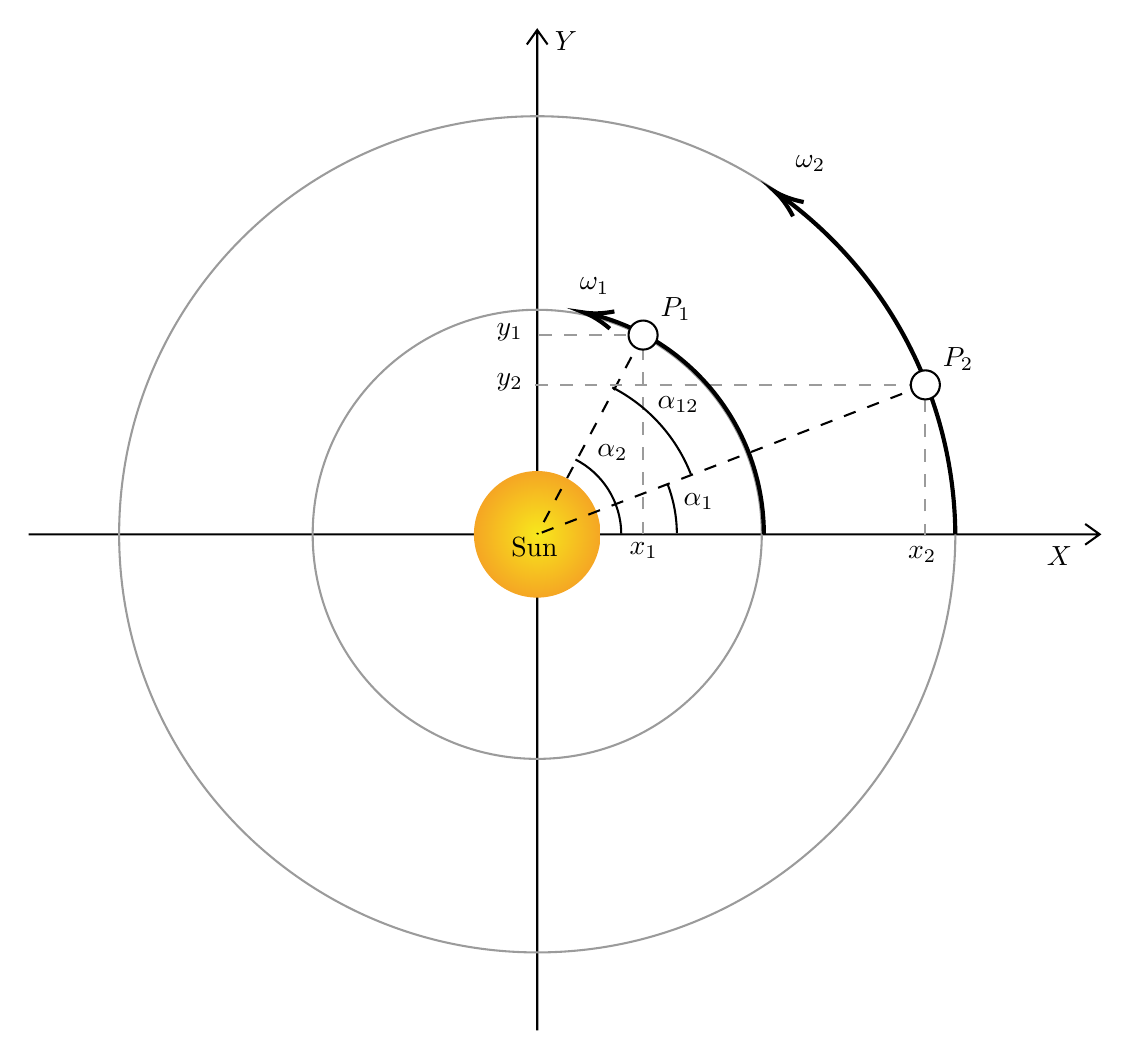
\begin{tikzpicture}[x=0.75pt,y=0.75pt,yscale=-1,xscale=1]
		%uncomment if require: \path (0,916); %set diagram left start at 0, and has height of 916
		
		% Gradient Info
		\tikzset {_1drpq3wcd/.code = {\pgfsetadditionalshadetransform{ \pgftransformshift{\pgfpoint{0 bp } { 0 bp }  }  \pgftransformscale{1 }  }}}
		\pgfdeclareradialshading{_cbpo3tqne}{\pgfpoint{0bp}{0bp}}{rgb(0bp)=(0.97,0.91,0.11);
		rgb(0bp)=(0.97,0.91,0.11);
		rgb(25bp)=(0.96,0.65,0.14);
		rgb(400bp)=(0.96,0.65,0.14)}
		\tikzset{every picture/.style={line width=0.75pt}} %set default line width to 0.75pt        
		
		%Shape: Axis 2D [id:dp5459429822341526] 
		\draw  (81,272) -- (597,272)(326,29) -- (326,511) (590,267) -- (597,272) -- (590,277) (321,36) -- (326,29) -- (331,36)  ;
		%Shape: Circle [id:dp5724433743250728] 
		\draw  [draw opacity=0][shading=_cbpo3tqne,_1drpq3wcd] (295.5,272) .. controls (295.5,255.16) and (309.16,241.5) .. (326,241.5) .. controls (342.84,241.5) and (356.5,255.16) .. (356.5,272) .. controls (356.5,288.84) and (342.84,302.5) .. (326,302.5) .. controls (309.16,302.5) and (295.5,288.84) .. (295.5,272) -- cycle ;
		%Shape: Circle [id:dp9612085741691925] 
		\draw  [color={rgb, 255:red, 155; green, 155; blue, 155 }  ,draw opacity=1 ] (217.81,272) .. controls (217.81,212.25) and (266.25,163.81) .. (326,163.81) .. controls (385.75,163.81) and (434.19,212.25) .. (434.19,272) .. controls (434.19,331.75) and (385.75,380.19) .. (326,380.19) .. controls (266.25,380.19) and (217.81,331.75) .. (217.81,272) -- cycle ;
		%Shape: Circle [id:dp9604349812821529] 
		\draw  [color={rgb, 255:red, 155; green, 155; blue, 155 }  ,draw opacity=1 ] (124.56,272) .. controls (124.56,160.75) and (214.75,70.56) .. (326,70.56) .. controls (437.25,70.56) and (527.44,160.75) .. (527.44,272) .. controls (527.44,383.25) and (437.25,473.44) .. (326,473.44) .. controls (214.75,473.44) and (124.56,383.25) .. (124.56,272) -- cycle ;
		%Straight Lines [id:da01676154486755732] 
		\draw  [dash pattern={on 4.5pt off 4.5pt}]  (513,200) -- (326,272) ;
		%Straight Lines [id:da7579199315844072] 
		\draw [color={rgb, 255:red, 155; green, 155; blue, 155 }  ,draw opacity=1 ] [dash pattern={on 4.5pt off 4.5pt}]  (377,272) -- (377,176) ;
		%Straight Lines [id:da31210870000960544] 
		\draw [color={rgb, 255:red, 155; green, 155; blue, 155 }  ,draw opacity=1 ] [dash pattern={on 4.5pt off 4.5pt}]  (327,176) -- (377,176) ;
		%Straight Lines [id:da8805604486506076] 
		\draw [color={rgb, 255:red, 155; green, 155; blue, 155 }  ,draw opacity=1 ] [dash pattern={on 4.5pt off 4.5pt}]  (513,273) -- (513,200) ;
		%Straight Lines [id:da05310757601195304] 
		\draw  [dash pattern={on 4.5pt off 4.5pt}]  (377,176) -- (326,272) ;
		%Straight Lines [id:da8497840415204332] 
		\draw [color={rgb, 255:red, 155; green, 155; blue, 155 }  ,draw opacity=1 ] [dash pattern={on 4.5pt off 4.5pt}]  (325,200) -- (502,200) -- (513,200) ;
		%Shape: Arc [id:dp14151095606464237] 
		\draw  [draw opacity=0][line width=1.5]  (348.35,165.1) .. controls (397.93,175.42) and (435.19,219.36) .. (435.19,272) -- (326,272) -- cycle ; \draw [line width=1.5]    (351.31,165.76) .. controls (399.41,177.18) and (435.19,220.41) .. (435.19,272) ;  \draw [shift={(348.35,165.1)}, rotate = 14.95] [color={rgb, 255:red, 0; green, 0; blue, 0 }  ][line width=1.5]    (14.21,-4.28) .. controls (9.04,-1.82) and (4.3,-0.39) .. (0,0) .. controls (4.3,0.39) and (9.04,1.82) .. (14.21,4.28)   ;
		%Shape: Circle [id:dp4598569311350238] 
		\draw  [fill={rgb, 255:red, 255; green, 255; blue, 255 }  ,fill opacity=1 ] (370,176) .. controls (370,172.13) and (373.13,169) .. (377,169) .. controls (380.87,169) and (384,172.13) .. (384,176) .. controls (384,179.87) and (380.87,183) .. (377,183) .. controls (373.13,183) and (370,179.87) .. (370,176) -- cycle ;
		%Shape: Arc [id:dp49990703839808104] 
		\draw  [draw opacity=0][line width=1.5]  (440.44,106.81) .. controls (492.58,143.34) and (526.84,203.65) .. (527.44,272) -- (323.65,273.85) -- cycle ; \draw [line width=1.5]    (443.55,109.03) .. controls (493.94,145.75) and (526.85,205.02) .. (527.44,272) ;  \draw [shift={(440.44,106.81)}, rotate = 36.88] [color={rgb, 255:red, 0; green, 0; blue, 0 }  ][line width=1.5]    (14.21,-4.28) .. controls (9.04,-1.82) and (4.3,-0.39) .. (0,0) .. controls (4.3,0.39) and (9.04,1.82) .. (14.21,4.28)   ;
		%Shape: Circle [id:dp7690267332912832] 
		\draw  [fill={rgb, 255:red, 255; green, 255; blue, 255 }  ,fill opacity=1 ] (506,200) .. controls (506,196.13) and (509.13,193) .. (513,193) .. controls (516.87,193) and (520,196.13) .. (520,200) .. controls (520,203.87) and (516.87,207) .. (513,207) .. controls (509.13,207) and (506,203.87) .. (506,200) -- cycle ;
		%Shape: Arc [id:dp8367130072247784] 
		\draw  [draw opacity=0][line width=0.75]  (388.81,247.84) .. controls (391.62,255.16) and (393.2,263.1) .. (393.27,271.39) -- (326,272) -- cycle ; \draw [line width=0.75]    (388.81,247.84) .. controls (391.62,255.16) and (393.2,263.1) .. (393.27,271.39) ;  
		%Shape: Arc [id:dp026100764172484192] 
		\draw  [draw opacity=0][line width=0.75]  (344.42,235.95) .. controls (357.41,242.6) and (366.33,256.07) .. (366.47,271.63) -- (326,272) -- cycle ; \draw [line width=0.75]    (344.42,235.95) .. controls (357.41,242.6) and (366.33,256.07) .. (366.47,271.63) ;  
		%Shape: Arc [id:dp7718348601097813] 
		\draw  [draw opacity=0][line width=0.75]  (362.17,201.22) .. controls (379.34,210.01) and (392.89,224.87) .. (399.99,242.96) -- (326,272) -- cycle ; \draw [line width=0.75]    (362.17,201.22) .. controls (379.34,210.01) and (392.89,224.87) .. (399.99,242.96) ;  
		
		% Text Node
		\draw (312,272) node [anchor=north west][inner sep=0.75pt]   [align=left] {Sun};
		% Text Node
		\draw (570,276.4) node [anchor=north west][inner sep=0.75pt]    {$X$};
		% Text Node
		\draw (333,28.4) node [anchor=north west][inner sep=0.75pt]    {$Y$};
		% Text Node
		\draw (503.19,276.4) node [anchor=north west][inner sep=0.75pt]    {$x_{2}$};
		% Text Node
		\draw (369,274.4) node [anchor=north west][inner sep=0.75pt]    {$x_{1}$};
		% Text Node
		\draw (305,169) node [anchor=north west][inner sep=0.75pt]    {$y_{1}$};
		% Text Node
		\draw (384,156.4) node [anchor=north west][inner sep=0.75pt]    {$P_{1}$};
		% Text Node
		\draw (395,251) node [anchor=north west][inner sep=0.75pt]    {$\alpha _{1}$};
		% Text Node
		\draw (520,180.4) node [anchor=north west][inner sep=0.75pt]    {$P_{2}$};
		% Text Node
		\draw (449,88) node [anchor=north west][inner sep=0.75pt]    {$\omega _{2}$};
		% Text Node
		\draw (345,147) node [anchor=north west][inner sep=0.75pt]    {$\omega _{1}$};
		% Text Node
		\draw (305,193) node [anchor=north west][inner sep=0.75pt]    {$y_{2}$};
		% Text Node
		\draw (353.5,227.4) node [anchor=north west][inner sep=0.75pt]    {$\alpha _{2}$};
		% Text Node
		\draw (382.5,204) node [anchor=north west][inner sep=0.75pt]    {$\alpha _{12}$};
		
		\end{tikzpicture}
		\caption{Basic scheme for determining the synodical period}
	\end{figure}
	where $P_1$ and $P_2$ are two planets which we will denote the respective sidereal  periods by $T_1$, $T_2$ and for which we deduce the angular velocities:
	
	If we take as zero time, the time when the two planets are both aligned with the $X$ axis and at the same side of this axis (so in "inferior conjunction"), then the angle between this axis and each of the planets is:
	
	We have respectively:
	
	We seek therefore all the instants $t$ where the following relation is satisfied for a fixed $\alpha_{12}$:
	
	Therefore it comes:
	
	If we look from time zero the first (next) conjunction ("superior conjunction"), this is equivalent to put that $\alpha_{12}=\pi$ and therefore that:
	
	If we look from time zero the first (next) conjunction ("inferior conjunction"),  this is equivalent to put that $\alpha_{12}=2\pi$ and therefore that:
	
	In the case where $\omega_2>\omega_1$ (typically Earth and one of its outer planets), the same reasoning leads us to:
	
	Here are some periods synodic and sidereal planets of the solar system relatively to Earth:
	\begin{table}[H]
	\begin{center}
		\definecolor{gris}{gray}{0.85}
			\begin{tabular}{|c|c|c|}
				\hline
				\multicolumn{1}{c}{\cellcolor[gray]{0.75}\textbf{Planet}} & 
\multicolumn{1}{c}{\cellcolor[gray]{0.75}\textbf{Synodic period [d]}} & 
\multicolumn{1}{c}{\cellcolor[gray]{0.75}\textbf{Sidelar period [d]}}  \\ \hline
		Mercury & $115.878$ & $87.969$\\ \hline
		Venus & $583.921$ & $224.709$\\ \hline
		March & $779.964$ & $686.960$\\ \hline
		Jupiter & $398.861$ & $4,335.355$\\ \hline
		Saturn & $378.094$ & $10,757.737$\\ \hline
		Uranus & $369.654$ & $30,708.160$\\ \hline
		Neptune & $367.486$ & $60,224.904$\\ \hline
	\end{tabular}
	\end{center}
	\caption{Various synodic and sidereal periods}
	\end{table}	
	As we can see from this table, we can make some of empirical observations:
	\begin{enumerate}
		\item For the inner planets: The closer we get to the Sun, the more the synodical period is short, indeed in the proved relation above, the more $T_1$ is small more $T$ decreases. So if there was a rotating planet very near the Sun, both sidereal and synodic periods are substantially equal.

		\item When we approach the Earth, the period increases. If there was a planet near to Earth, we would then have $T_1$ value close to $T_2$ value and the synodical period would be very large.

		\item For the outer planets: The synodic period decreases when the planet is farther from the Earth and approaches terrestrial sidereal period of $365$ days. We see well for Neptune, if we discovered a planet even further its synodic period would approach even more the $365$ days.
	\end{enumerate}
	
	\pagebreak
	\subsubsection{Planet's apparent retrograde motion}
	The "\NewTerm{retrograde motion}\index{retrograde motion}" of a planet is an apparent motion of this planet which gives the impression that it stop in his path in the "direct movement" to start reversing. This phenomenon is the result of the difference between the revolution speed of the planet and the Earth around the Sun.

	The example below shows roughly what a terrestrial observer (blue discs) can be observed by monitoring month after month, the apparent motion of Mars (brown discs):
	\begin{figure}[H]
		\centering
		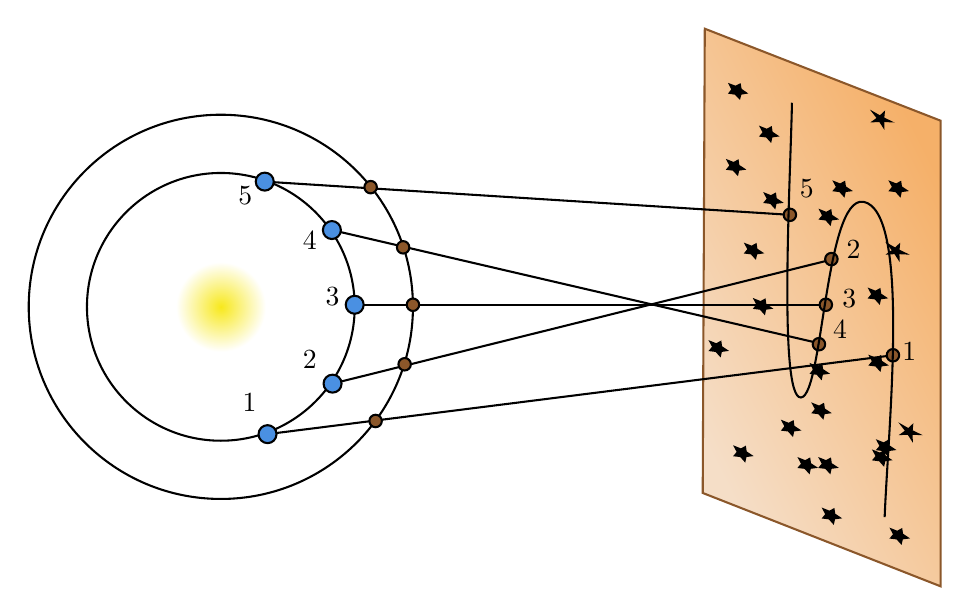
\begin{tikzpicture}[x=0.75pt,y=0.75pt,yscale=-1,xscale=1]
		%uncomment if require: \path (0,712); %set diagram left start at 0, and has height of 712

		% Gradient Info
		\tikzset {_ni6y6cjbw/.code = {\pgfsetadditionalshadetransform{ \pgftransformshift{\pgfpoint{0 bp } { 0 bp }  }  \pgftransformrotate{-310 }  \pgftransformscale{2 }  }}}
		\pgfdeclarehorizontalshading{_9s6tfjwzs}{150bp}{rgb(0bp)=(0.96,0.87,0.78);
		rgb(37.5bp)=(0.96,0.87,0.78);
		rgb(62.5bp)=(0.96,0.69,0.41);
		rgb(100bp)=(0.96,0.69,0.41)}
		
		% Gradient Info
		  
		\tikzset {_62kw9gixe/.code = {\pgfsetadditionalshadetransform{ \pgftransformshift{\pgfpoint{0 bp } { 0 bp }  }  \pgftransformscale{1.54 }  }}}
		\pgfdeclareradialshading{_72ri2gi5o}{\pgfpoint{0bp}{0bp}}{rgb(0bp)=(0.97,0.91,0.11);
		rgb(0bp)=(0.97,0.91,0.11);
		rgb(14.017857142857142bp)=(1,1,1);
		rgb(400bp)=(1,1,1)}
				
		%Shape: Polygon [id:ds8541353001148053] 
		\path  [shading=_9s6tfjwzs,_ni6y6cjbw] (371.17,48) -- (484.83,92.33) -- (484.83,212.33) -- (484.83,316.67) -- (370.17,271.67) -- cycle ; % for fading 
		 \draw  [color={rgb, 255:red, 139; green, 87; blue, 42 }  ,draw opacity=1 ] (371.17,48) -- (484.83,92.33) -- (484.83,212.33) -- (484.83,316.67) -- (370.17,271.67) -- cycle ; % for border 
		
		%Straight Lines [id:da07451099325639521] 
		\draw    (159.17,121.67) -- (412.17,137.67) ;
		%Straight Lines [id:da7804726949466878] 
		\draw    (191.5,145) -- (428.17,200) ;
		%Straight Lines [id:da519547051657969] 
		\draw    (202.5,181) -- (429.5,181) ;
		%Straight Lines [id:da19751671093574408] 
		\draw    (191.83,219) -- (433.17,159) ;
		%Straight Lines [id:da8590646002516045] 
		\draw    (160.5,243.33) -- (461.83,205.33) ;
		%Shape: Circle [id:dp2706888472046287] 
		\draw  [draw opacity=0][shading=_72ri2gi5o,_62kw9gixe] (113,182) .. controls (113,168.19) and (124.19,157) .. (138,157) .. controls (151.81,157) and (163,168.19) .. (163,182) .. controls (163,195.81) and (151.81,207) .. (138,207) .. controls (124.19,207) and (113,195.81) .. (113,182) -- cycle ;
		%Shape: Circle [id:dp01500239420106153] 
		\draw   (73.5,182) .. controls (73.5,146.38) and (102.38,117.5) .. (138,117.5) .. controls (173.62,117.5) and (202.5,146.38) .. (202.5,182) .. controls (202.5,217.62) and (173.62,246.5) .. (138,246.5) .. controls (102.38,246.5) and (73.5,217.62) .. (73.5,182) -- cycle ;
		%Shape: Circle [id:dp025367530788808823] 
		\draw   (45.44,182) .. controls (45.44,130.88) and (86.88,89.44) .. (138,89.44) .. controls (189.12,89.44) and (230.56,130.88) .. (230.56,182) .. controls (230.56,233.12) and (189.12,274.56) .. (138,274.56) .. controls (86.88,274.56) and (45.44,233.12) .. (45.44,182) -- cycle ;
		%Shape: Circle [id:dp7804672188082797] 
		\draw  [fill={rgb, 255:red, 74; green, 144; blue, 226 }  ,fill opacity=1 ] (154.83,121.67) .. controls (154.83,119.27) and (156.77,117.33) .. (159.17,117.33) .. controls (161.56,117.33) and (163.5,119.27) .. (163.5,121.67) .. controls (163.5,124.06) and (161.56,126) .. (159.17,126) .. controls (156.77,126) and (154.83,124.06) .. (154.83,121.67) -- cycle ;
		%Shape: Circle [id:dp28907899423216343] 
		\draw  [fill={rgb, 255:red, 74; green, 144; blue, 226 }  ,fill opacity=1 ] (187.17,145) .. controls (187.17,142.61) and (189.11,140.67) .. (191.5,140.67) .. controls (193.89,140.67) and (195.83,142.61) .. (195.83,145) .. controls (195.83,147.39) and (193.89,149.33) .. (191.5,149.33) .. controls (189.11,149.33) and (187.17,147.39) .. (187.17,145) -- cycle ;
		%Shape: Circle [id:dp766295540506932] 
		\draw  [fill={rgb, 255:red, 74; green, 144; blue, 226 }  ,fill opacity=1 ] (198.17,181) .. controls (198.17,178.61) and (200.11,176.67) .. (202.5,176.67) .. controls (204.89,176.67) and (206.83,178.61) .. (206.83,181) .. controls (206.83,183.39) and (204.89,185.33) .. (202.5,185.33) .. controls (200.11,185.33) and (198.17,183.39) .. (198.17,181) -- cycle ;
		%Shape: Circle [id:dp8140598497564899] 
		\draw  [fill={rgb, 255:red, 74; green, 144; blue, 226 }  ,fill opacity=1 ] (187.5,219) .. controls (187.5,216.61) and (189.44,214.67) .. (191.83,214.67) .. controls (194.23,214.67) and (196.17,216.61) .. (196.17,219) .. controls (196.17,221.39) and (194.23,223.33) .. (191.83,223.33) .. controls (189.44,223.33) and (187.5,221.39) .. (187.5,219) -- cycle ;
		%Shape: Circle [id:dp21080342593265433] 
		\draw  [fill={rgb, 255:red, 74; green, 144; blue, 226 }  ,fill opacity=1 ] (156.17,243.33) .. controls (156.17,240.94) and (158.11,239) .. (160.5,239) .. controls (162.89,239) and (164.83,240.94) .. (164.83,243.33) .. controls (164.83,245.73) and (162.89,247.67) .. (160.5,247.67) .. controls (158.11,247.67) and (156.17,245.73) .. (156.17,243.33) -- cycle ;
		%Shape: Circle [id:dp9548438696764499] 
		\draw  [fill={rgb, 255:red, 139; green, 87; blue, 42 }  ,fill opacity=1 ] (207.17,124.33) .. controls (207.17,122.68) and (208.51,121.33) .. (210.17,121.33) .. controls (211.82,121.33) and (213.17,122.68) .. (213.17,124.33) .. controls (213.17,125.99) and (211.82,127.33) .. (210.17,127.33) .. controls (208.51,127.33) and (207.17,125.99) .. (207.17,124.33) -- cycle ;
		%Shape: Circle [id:dp888012370144196] 
		\draw  [fill={rgb, 255:red, 139; green, 87; blue, 42 }  ,fill opacity=1 ] (222.83,153.33) .. controls (222.83,151.68) and (224.18,150.33) .. (225.83,150.33) .. controls (227.49,150.33) and (228.83,151.68) .. (228.83,153.33) .. controls (228.83,154.99) and (227.49,156.33) .. (225.83,156.33) .. controls (224.18,156.33) and (222.83,154.99) .. (222.83,153.33) -- cycle ;
		%Shape: Circle [id:dp4285995465584147] 
		\draw  [fill={rgb, 255:red, 139; green, 87; blue, 42 }  ,fill opacity=1 ] (227.56,181) .. controls (227.56,179.34) and (228.91,178) .. (230.56,178) .. controls (232.22,178) and (233.56,179.34) .. (233.56,181) .. controls (233.56,182.66) and (232.22,184) .. (230.56,184) .. controls (228.91,184) and (227.56,182.66) .. (227.56,181) -- cycle ;
		%Shape: Circle [id:dp6048183661988833] 
		\draw  [fill={rgb, 255:red, 139; green, 87; blue, 42 }  ,fill opacity=1 ] (223.56,209.67) .. controls (223.56,208.01) and (224.91,206.67) .. (226.56,206.67) .. controls (228.22,206.67) and (229.56,208.01) .. (229.56,209.67) .. controls (229.56,211.32) and (228.22,212.67) .. (226.56,212.67) .. controls (224.91,212.67) and (223.56,211.32) .. (223.56,209.67) -- cycle ;
		%Shape: Circle [id:dp8181982278752085] 
		\draw  [fill={rgb, 255:red, 139; green, 87; blue, 42 }  ,fill opacity=1 ] (209.56,237) .. controls (209.56,235.34) and (210.91,234) .. (212.56,234) .. controls (214.22,234) and (215.56,235.34) .. (215.56,237) .. controls (215.56,238.66) and (214.22,240) .. (212.56,240) .. controls (210.91,240) and (209.56,238.66) .. (209.56,237) -- cycle ;
		%Shape: Circle [id:dp10123219902889713] 
		\draw  [fill={rgb, 255:red, 139; green, 87; blue, 42 }  ,fill opacity=1 ] (409.17,137.67) .. controls (409.17,136.01) and (410.51,134.67) .. (412.17,134.67) .. controls (413.82,134.67) and (415.17,136.01) .. (415.17,137.67) .. controls (415.17,139.32) and (413.82,140.67) .. (412.17,140.67) .. controls (410.51,140.67) and (409.17,139.32) .. (409.17,137.67) -- cycle ;
		%Shape: Circle [id:dp7172832009675363] 
		\draw  [fill={rgb, 255:red, 139; green, 87; blue, 42 }  ,fill opacity=1 ] (429.17,159) .. controls (429.17,157.34) and (430.51,156) .. (432.17,156) .. controls (433.82,156) and (435.17,157.34) .. (435.17,159) .. controls (435.17,160.66) and (433.82,162) .. (432.17,162) .. controls (430.51,162) and (429.17,160.66) .. (429.17,159) -- cycle ;
		%Shape: Circle [id:dp010644652182668635] 
		\draw  [fill={rgb, 255:red, 139; green, 87; blue, 42 }  ,fill opacity=1 ] (426.5,181) .. controls (426.5,179.34) and (427.84,178) .. (429.5,178) .. controls (431.16,178) and (432.5,179.34) .. (432.5,181) .. controls (432.5,182.66) and (431.16,184) .. (429.5,184) .. controls (427.84,184) and (426.5,182.66) .. (426.5,181) -- cycle ;
		%Shape: Circle [id:dp058103181928748526] 
		\draw  [fill={rgb, 255:red, 139; green, 87; blue, 42 }  ,fill opacity=1 ] (423.17,200) .. controls (423.17,198.34) and (424.51,197) .. (426.17,197) .. controls (427.82,197) and (429.17,198.34) .. (429.17,200) .. controls (429.17,201.66) and (427.82,203) .. (426.17,203) .. controls (424.51,203) and (423.17,201.66) .. (423.17,200) -- cycle ;
		%Shape: Circle [id:dp6478836419654275] 
		\draw  [fill={rgb, 255:red, 139; green, 87; blue, 42 }  ,fill opacity=1 ] (458.83,205.33) .. controls (458.83,203.68) and (460.18,202.33) .. (461.83,202.33) .. controls (463.49,202.33) and (464.83,203.68) .. (464.83,205.33) .. controls (464.83,206.99) and (463.49,208.33) .. (461.83,208.33) .. controls (460.18,208.33) and (458.83,206.99) .. (458.83,205.33) -- cycle ;
		%Curve Lines [id:da36287602823884346] 
		\draw    (413.17,83.67) .. controls (412.5,119) and (406.5,226.33) .. (417.5,225.67) .. controls (428.5,225) and (429.17,122) .. (449.5,132) .. controls (469.83,142) and (459.5,240.33) .. (457.83,283.33) ;
		%Shape: Star [id:dp866386479336466] 
		\draw  [fill={rgb, 255:red, 0; green, 0; blue, 0 }  ,fill opacity=1 ] (387.86,81.33) -- (388.4,79.32) -- (390.82,78.91) -- (388.46,77.27) -- (388.04,75) -- (386.04,76) -- (383.37,75) -- (384.49,77.27) -- (383.25,78.91) -- (385.95,79.32) -- cycle ;
		%Shape: Star [id:dp015393464208243834] 
		\draw  [fill={rgb, 255:red, 0; green, 0; blue, 0 }  ,fill opacity=1 ] (457.19,95) -- (457.1,92.44) -- (460.15,92.58) -- (457.14,91.14) -- (457.38,88.67) -- (455.6,90.33) -- (452.7,88.67) -- (454.62,91.14) -- (452.58,92.58) -- (455.54,92.44) -- cycle ;
		%Shape: Star [id:dp8086191372267226] 
		\draw  [fill={rgb, 255:red, 0; green, 0; blue, 0 }  ,fill opacity=1 ] (402.86,102) -- (403.32,99.92) -- (405.82,99.58) -- (403.37,97.96) -- (403.04,95.67) -- (401.07,96.75) -- (398.37,95.67) -- (399.59,97.96) -- (398.25,99.58) -- (400.98,99.92) -- cycle ;
		%Shape: Star [id:dp2713126161044501] 
		\draw  [fill={rgb, 255:red, 0; green, 0; blue, 0 }  ,fill opacity=1 ] (386.86,118) -- (387.32,115.92) -- (389.82,115.58) -- (387.37,113.96) -- (387.04,111.67) -- (385.07,112.75) -- (382.37,111.67) -- (383.59,113.96) -- (382.25,115.58) -- (384.98,115.92) -- cycle ;
		%Shape: Star [id:dp23138514457294868] 
		\draw  [fill={rgb, 255:red, 0; green, 0; blue, 0 }  ,fill opacity=1 ] (404.86,134) -- (405.32,131.92) -- (407.82,131.58) -- (405.37,129.96) -- (405.04,127.67) -- (403.07,128.75) -- (400.37,127.67) -- (401.59,129.96) -- (400.25,131.58) -- (402.98,131.92) -- cycle ;
		%Shape: Star [id:dp501829984169061] 
		\draw  [fill={rgb, 255:red, 0; green, 0; blue, 0 }  ,fill opacity=1 ] (431.52,142) -- (431.98,139.92) -- (434.48,139.58) -- (432.04,137.96) -- (431.71,135.67) -- (429.74,136.75) -- (427.03,135.67) -- (428.26,137.96) -- (426.92,139.58) -- (429.65,139.92) -- cycle ;
		%Shape: Star [id:dp005626227320733257] 
		\draw  [fill={rgb, 255:red, 0; green, 0; blue, 0 }  ,fill opacity=1 ] (438.19,128.33) -- (438.65,126.25) -- (441.15,125.91) -- (438.71,124.29) -- (438.38,122) -- (436.41,123.08) -- (433.7,122) -- (434.92,124.29) -- (433.58,125.91) -- (436.31,126.25) -- cycle ;
		%Shape: Star [id:dp4072778228163567] 
		\draw  [fill={rgb, 255:red, 0; green, 0; blue, 0 }  ,fill opacity=1 ] (465.19,128.33) -- (465.65,126.25) -- (468.15,125.91) -- (465.71,124.29) -- (465.38,122) -- (463.41,123.08) -- (460.7,122) -- (461.92,124.29) -- (460.58,125.91) -- (463.31,126.25) -- cycle ;
		%Shape: Star [id:dp6472114222537886] 
		\draw  [fill={rgb, 255:red, 0; green, 0; blue, 0 }  ,fill opacity=1 ] (464.52,158.67) -- (464.43,156.11) -- (467.48,156.25) -- (464.47,154.81) -- (464.71,152.34) -- (462.94,154) -- (460.03,152.34) -- (461.95,154.81) -- (459.92,156.25) -- (462.87,156.11) -- cycle ;
		%Shape: Star [id:dp6998498624265717] 
		\draw  [fill={rgb, 255:red, 0; green, 0; blue, 0 }  ,fill opacity=1 ] (455.19,180) -- (455.65,177.92) -- (458.15,177.58) -- (455.71,175.96) -- (455.38,173.67) -- (453.41,174.75) -- (450.7,173.67) -- (451.92,175.96) -- (450.58,177.58) -- (453.31,177.92) -- cycle ;
		%Shape: Star [id:dp5337030557289695] 
		\draw  [fill={rgb, 255:red, 0; green, 0; blue, 0 }  ,fill opacity=1 ] (399.86,185) -- (400.32,182.92) -- (402.82,182.58) -- (400.37,180.96) -- (400.04,178.67) -- (398.07,179.75) -- (395.37,178.67) -- (396.59,180.96) -- (395.25,182.58) -- (397.98,182.92) -- cycle ;
		%Shape: Star [id:dp40021992461469025] 
		\draw  [fill={rgb, 255:red, 0; green, 0; blue, 0 }  ,fill opacity=1 ] (395.52,158.33) -- (395.98,156.25) -- (398.48,155.91) -- (396.04,154.29) -- (395.71,152) -- (393.74,153.08) -- (391.03,152) -- (392.26,154.29) -- (390.92,155.91) -- (393.65,156.25) -- cycle ;
		%Shape: Star [id:dp41042001861475685] 
		\draw  [fill={rgb, 255:red, 0; green, 0; blue, 0 }  ,fill opacity=1 ] (378.52,205.33) -- (378.98,203.25) -- (381.48,202.91) -- (379.04,201.29) -- (378.71,199) -- (376.74,200.08) -- (374.03,199) -- (375.26,201.29) -- (373.92,202.91) -- (376.65,203.25) -- cycle ;
		%Shape: Star [id:dp5814490159128156] 
		\draw  [fill={rgb, 255:red, 0; green, 0; blue, 0 }  ,fill opacity=1 ] (427.19,216.33) -- (427.65,214.25) -- (430.15,213.91) -- (427.71,212.29) -- (427.38,210) -- (425.41,211.08) -- (422.7,210) -- (423.92,212.29) -- (422.58,213.91) -- (425.31,214.25) -- cycle ;
		%Shape: Star [id:dp7241103328832841] 
		\draw  [fill={rgb, 255:red, 0; green, 0; blue, 0 }  ,fill opacity=1 ] (455.52,212.33) -- (455.98,210.25) -- (458.48,209.91) -- (456.04,208.29) -- (455.71,206) -- (453.74,207.08) -- (451.03,206) -- (452.26,208.29) -- (450.92,209.91) -- (453.65,210.25) -- cycle ;
		%Shape: Star [id:dp19471113347685565] 
		\draw  [fill={rgb, 255:red, 0; green, 0; blue, 0 }  ,fill opacity=1 ] (470.86,245.67) -- (470.77,243.11) -- (473.82,243.25) -- (470.81,241.81) -- (471.04,239.34) -- (469.27,241) -- (466.37,239.34) -- (468.28,241.81) -- (466.25,243.25) -- (469.21,243.11) -- cycle ;
		%Shape: Star [id:dp8097084471352554] 
		\draw  [fill={rgb, 255:red, 0; green, 0; blue, 0 }  ,fill opacity=1 ] (459.16,253.08) -- (459.62,251) -- (462.12,250.66) -- (459.68,249.04) -- (459.35,246.75) -- (457.38,247.83) -- (454.67,246.75) -- (455.9,249.04) -- (454.56,250.66) -- (457.28,251) -- cycle ;
		%Shape: Star [id:dp7163482706481454] 
		\draw  [fill={rgb, 255:red, 0; green, 0; blue, 0 }  ,fill opacity=1 ] (457.28,258) -- (457.74,255.91) -- (460.24,255.58) -- (457.8,253.96) -- (457.47,251.67) -- (455.5,252.75) -- (452.79,251.67) -- (454.02,253.96) -- (452.68,255.58) -- (455.41,255.91) -- cycle ;
		%Shape: Star [id:dp39472478937111166] 
		\draw  [fill={rgb, 255:red, 0; green, 0; blue, 0 }  ,fill opacity=1 ] (465.71,295.66) -- (466.17,293.58) -- (468.67,293.25) -- (466.23,291.62) -- (465.89,289.33) -- (463.92,290.41) -- (461.22,289.33) -- (462.44,291.62) -- (461.1,293.25) -- (463.83,293.58) -- cycle ;
		%Shape: Star [id:dp9115061565087199] 
		\draw  [fill={rgb, 255:red, 0; green, 0; blue, 0 }  ,fill opacity=1 ] (433.04,286) -- (433.5,283.91) -- (436,283.58) -- (433.56,281.96) -- (433.23,279.67) -- (431.26,280.75) -- (428.55,279.67) -- (429.78,281.96) -- (428.44,283.58) -- (431.16,283.91) -- cycle ;
		%Shape: Star [id:dp3169299400425727] 
		\draw  [fill={rgb, 255:red, 0; green, 0; blue, 0 }  ,fill opacity=1 ] (431.38,261.66) -- (431.84,259.58) -- (434.34,259.25) -- (431.89,257.62) -- (431.56,255.33) -- (429.59,256.41) -- (426.89,255.33) -- (428.11,257.62) -- (426.77,259.25) -- (429.5,259.58) -- cycle ;
		%Shape: Star [id:dp2880812091604008] 
		\draw  [fill={rgb, 255:red, 0; green, 0; blue, 0 }  ,fill opacity=1 ] (421.38,261.66) -- (421.84,259.58) -- (424.34,259.25) -- (421.89,257.62) -- (421.56,255.33) -- (419.59,256.41) -- (416.89,255.33) -- (418.11,257.62) -- (416.77,259.25) -- (419.5,259.58) -- cycle ;
		%Shape: Star [id:dp8825750561297709] 
		\draw  [fill={rgb, 255:red, 0; green, 0; blue, 0 }  ,fill opacity=1 ] (428.04,235.33) -- (428.5,233.25) -- (431,232.91) -- (428.56,231.29) -- (428.23,229) -- (426.26,230.08) -- (423.55,229) -- (424.78,231.29) -- (423.44,232.91) -- (426.16,233.25) -- cycle ;
		%Shape: Star [id:dp2449171351888122] 
		\draw  [fill={rgb, 255:red, 0; green, 0; blue, 0 }  ,fill opacity=1 ] (413.38,243.66) -- (413.84,241.58) -- (416.34,241.25) -- (413.89,239.62) -- (413.56,237.33) -- (411.59,238.41) -- (408.89,237.33) -- (410.11,239.62) -- (408.77,241.25) -- (411.5,241.58) -- cycle ;
		%Shape: Star [id:dp5413168509265052] 
		\draw  [fill={rgb, 255:red, 0; green, 0; blue, 0 }  ,fill opacity=1 ] (390.38,256) -- (390.84,253.91) -- (393.34,253.58) -- (390.89,251.96) -- (390.56,249.67) -- (388.59,250.75) -- (385.89,249.67) -- (387.11,251.96) -- (385.77,253.58) -- (388.5,253.91) -- cycle ;
		
		
		% Text Node
		\draw (145,122.4) node [anchor=north west][inner sep=0.75pt]    {$5$};
		% Text Node
		\draw (176,144.4) node [anchor=north west][inner sep=0.75pt]    {$4$};
		% Text Node
		\draw (187,171.4) node [anchor=north west][inner sep=0.75pt]    {$3$};
		% Text Node
		\draw (176,201.4) node [anchor=north west][inner sep=0.75pt]    {$2$};
		% Text Node
		\draw (147,222.4) node [anchor=north west][inner sep=0.75pt]    {$1$};
		% Text Node
		\draw (464.83,197.73) node [anchor=north west][inner sep=0.75pt]    {$1$};
		% Text Node
		\draw (438,148.4) node [anchor=north west][inner sep=0.75pt]    {$2$};
		% Text Node
		\draw (436,172.4) node [anchor=north west][inner sep=0.75pt]    {$3$};
		% Text Node
		\draw (431.5,187.4) node [anchor=north west][inner sep=0.75pt]    {$4$};
		% Text Node
		\draw (415.5,119.4) node [anchor=north west][inner sep=0.75pt]    {$5$};
		
		\end{tikzpicture}
		\caption[Retrograde motion principle]{Retrograde motion principle (source: Wikipedia)}
	\end{figure}
	Or more explicitly (in the legend of the figure below, the years are given based on the holocene calendar):
	\begin{figure}[H]
		\centering
		\includegraphics[scale=0.75]{img/cosmology/retrograde_motion_mars.jpg}
		\vspace*{3mm}	
		\caption[Apparent retrograde motion of Mars in 12003 as seen from Earth]{Apparent retrograde motion of Mars in 12003 as seen from Earth\\(source: Wikipedia, author: Eugene Alvin Villar)}
	\end{figure}
	To study this phenomenon mathematically, we will consider the following figure:
	\begin{figure}[H]
		\centering
		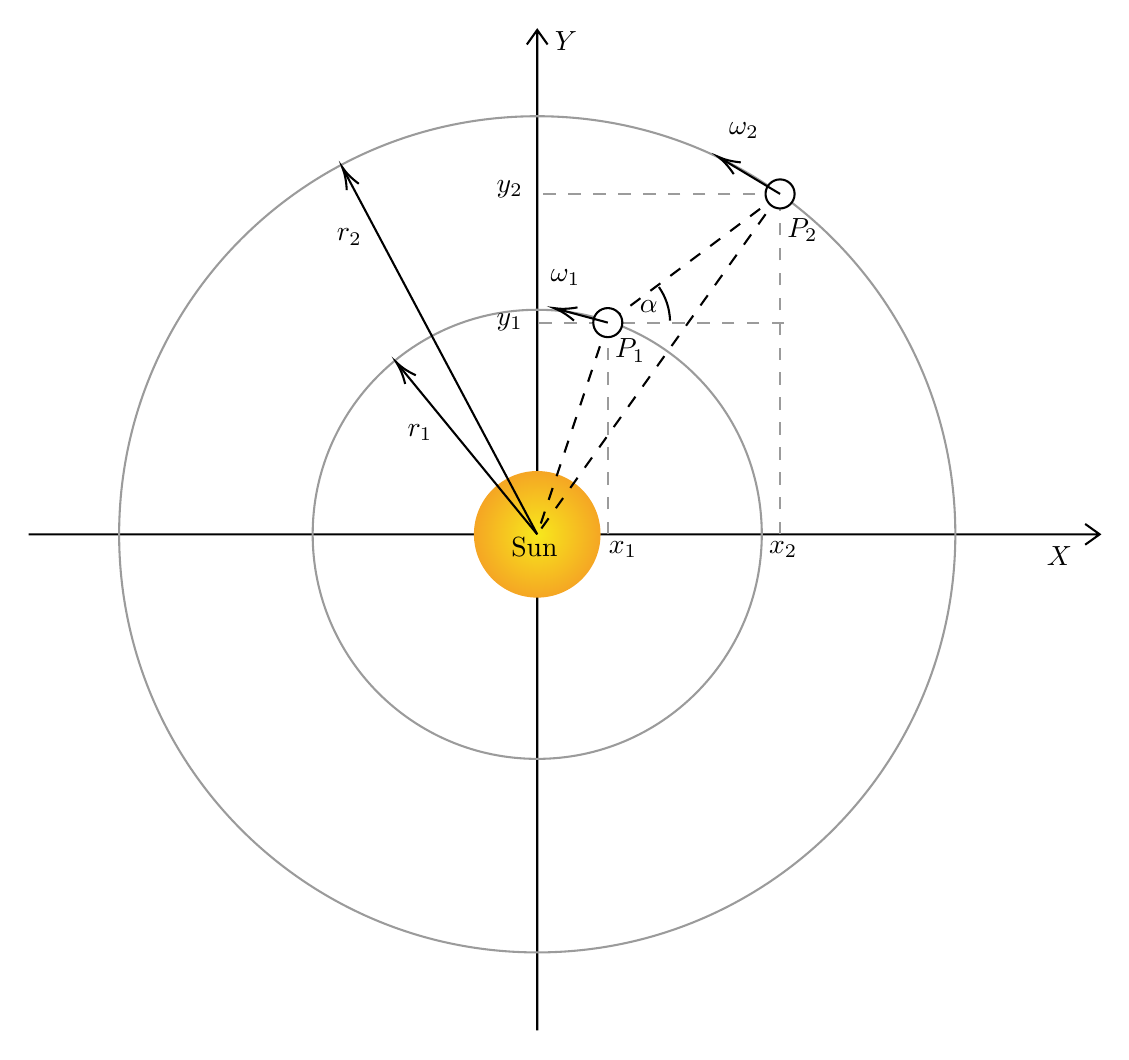
\begin{tikzpicture}[x=0.75pt,y=0.75pt,yscale=-1,xscale=1]
		%uncomment if require: \path (0,1215); %set diagram left start at 0, and has height of 1215
		
		% Gradient Info
  
		\tikzset {_mc0sd1mt4/.code = {\pgfsetadditionalshadetransform{ \pgftransformshift{\pgfpoint{0 bp } { 0 bp }  }  \pgftransformscale{1 }  }}}
		\pgfdeclareradialshading{_bzu0ltxui}{\pgfpoint{0bp}{0bp}}{rgb(0bp)=(0.97,0.91,0.11);
		rgb(0bp)=(0.97,0.91,0.11);
		rgb(25bp)=(0.96,0.65,0.14);
		rgb(400bp)=(0.96,0.65,0.14)}
		
		%Straight Lines [id:da04281355948589405] 
		\draw [color={rgb, 255:red, 155; green, 155; blue, 155 }  ,draw opacity=1 ] [dash pattern={on 4.5pt off 4.5pt}]  (440,166) -- (355,166) ;
		%Shape: Axis 2D [id:dp38783749104621434] 
		\draw  (76,268) -- (592,268)(321,25) -- (321,507) (585,263) -- (592,268) -- (585,273) (316,32) -- (321,25) -- (326,32)  ;
		%Shape: Circle [id:dp5244757831866251] 
		\draw  [draw opacity=0][shading=_bzu0ltxui,_mc0sd1mt4] (290.5,268) .. controls (290.5,251.16) and (304.16,237.5) .. (321,237.5) .. controls (337.84,237.5) and (351.5,251.16) .. (351.5,268) .. controls (351.5,284.84) and (337.84,298.5) .. (321,298.5) .. controls (304.16,298.5) and (290.5,284.84) .. (290.5,268) -- cycle ;
		%Shape: Circle [id:dp4316445775118811] 
		\draw  [color={rgb, 255:red, 155; green, 155; blue, 155 }  ,draw opacity=1 ] (212.81,268) .. controls (212.81,208.25) and (261.25,159.81) .. (321,159.81) .. controls (380.75,159.81) and (429.19,208.25) .. (429.19,268) .. controls (429.19,327.75) and (380.75,376.19) .. (321,376.19) .. controls (261.25,376.19) and (212.81,327.75) .. (212.81,268) -- cycle ;
		%Shape: Circle [id:dp28001572621578585] 
		\draw  [color={rgb, 255:red, 155; green, 155; blue, 155 }  ,draw opacity=1 ] (119.56,268) .. controls (119.56,156.75) and (209.75,66.56) .. (321,66.56) .. controls (432.25,66.56) and (522.44,156.75) .. (522.44,268) .. controls (522.44,379.25) and (432.25,469.44) .. (321,469.44) .. controls (209.75,469.44) and (119.56,379.25) .. (119.56,268) -- cycle ;
		%Straight Lines [id:da804153013274191] 
		\draw    (321,268) -- (254.27,186.55) ;
		\draw [shift={(253,185)}, rotate = 50.67] [color={rgb, 255:red, 0; green, 0; blue, 0 }  ][line width=0.75]    (10.93,-3.29) .. controls (6.95,-1.4) and (3.31,-0.3) .. (0,0) .. controls (3.31,0.3) and (6.95,1.4) .. (10.93,3.29)   ;
		%Straight Lines [id:da3951530386786708] 
		\draw    (321,268) -- (227.94,92.77) ;
		\draw [shift={(227,91)}, rotate = 62.03] [color={rgb, 255:red, 0; green, 0; blue, 0 }  ][line width=0.75]    (10.93,-3.29) .. controls (6.95,-1.4) and (3.31,-0.3) .. (0,0) .. controls (3.31,0.3) and (6.95,1.4) .. (10.93,3.29)   ;
		%Straight Lines [id:da0910173224313986] 
		\draw  [dash pattern={on 4.5pt off 4.5pt}]  (355,166) -- (321,268) ;
		%Straight Lines [id:da10760937901968215] 
		\draw  [dash pattern={on 4.5pt off 4.5pt}]  (438,104) -- (321,268) ;
		%Straight Lines [id:da6572575883258371] 
		\draw  [dash pattern={on 4.5pt off 4.5pt}]  (438,104) -- (355,166) ;
		%Straight Lines [id:da1662019804711361] 
		\draw [color={rgb, 255:red, 155; green, 155; blue, 155 }  ,draw opacity=1 ] [dash pattern={on 4.5pt off 4.5pt}]  (438,104) -- (322,104) ;
		%Straight Lines [id:da22175825075554667] 
		\draw [color={rgb, 255:red, 155; green, 155; blue, 155 }  ,draw opacity=1 ] [dash pattern={on 4.5pt off 4.5pt}]  (438,268) -- (438,104) ;
		%Shape: Circle [id:dp5001486403299928] 
		\draw  [fill={rgb, 255:red, 255; green, 255; blue, 255 }  ,fill opacity=1 ] (431,104) .. controls (431,100.13) and (434.13,97) .. (438,97) .. controls (441.87,97) and (445,100.13) .. (445,104) .. controls (445,107.87) and (441.87,111) .. (438,111) .. controls (434.13,111) and (431,107.87) .. (431,104) -- cycle ;
		%Straight Lines [id:da0489247519439191] 
		\draw [color={rgb, 255:red, 155; green, 155; blue, 155 }  ,draw opacity=1 ] [dash pattern={on 4.5pt off 4.5pt}]  (355,268) -- (355,166) ;
		%Straight Lines [id:da333153221215301] 
		\draw [color={rgb, 255:red, 155; green, 155; blue, 155 }  ,draw opacity=1 ] [dash pattern={on 4.5pt off 4.5pt}]  (322,166) -- (355,166) ;
		%Shape: Circle [id:dp9047195286217191] 
		\draw  [fill={rgb, 255:red, 255; green, 255; blue, 255 }  ,fill opacity=1 ] (348,166) .. controls (348,162.13) and (351.13,159) .. (355,159) .. controls (358.87,159) and (362,162.13) .. (362,166) .. controls (362,169.87) and (358.87,173) .. (355,173) .. controls (351.13,173) and (348,169.87) .. (348,166) -- cycle ;
		%Shape: Arc [id:dp2322584795245637] 
		\draw  [draw opacity=0] (379.63,148.87) .. controls (382.85,153.49) and (384.8,159.05) .. (384.99,165.06) -- (355,166) -- cycle ; \draw   (379.63,148.87) .. controls (382.85,153.49) and (384.8,159.05) .. (384.99,165.06) ;  
		%Straight Lines [id:da8467701849112594] 
		\draw    (438,104) -- (409.71,87.03) ;
		\draw [shift={(408,86)}, rotate = 30.96] [color={rgb, 255:red, 0; green, 0; blue, 0 }  ][line width=0.75]    (10.93,-3.29) .. controls (6.95,-1.4) and (3.31,-0.3) .. (0,0) .. controls (3.31,0.3) and (6.95,1.4) .. (10.93,3.29)   ;
		%Straight Lines [id:da8914982498961315] 
		\draw    (355,166) -- (330.93,159.52) ;
		\draw [shift={(329,159)}, rotate = 15.07] [color={rgb, 255:red, 0; green, 0; blue, 0 }  ][line width=0.75]    (10.93,-3.29) .. controls (6.95,-1.4) and (3.31,-0.3) .. (0,0) .. controls (3.31,0.3) and (6.95,1.4) .. (10.93,3.29)   ;
		
		% Text Node
		\draw (307,268) node [anchor=north west][inner sep=0.75pt]   [align=left] {Sun};
		% Text Node
		\draw (565,272.4) node [anchor=north west][inner sep=0.75pt]    {$X$};
		% Text Node
		\draw (328,24.4) node [anchor=north west][inner sep=0.75pt]    {$Y$};
		% Text Node
		\draw (223,119.4) node [anchor=north west][inner sep=0.75pt]    {$r_{2}$};
		% Text Node
		\draw (257,213.4) node [anchor=north west][inner sep=0.75pt]    {$r_{1}$};
		% Text Node
		\draw (300,96) node [anchor=north west][inner sep=0.75pt]    {$y_{2}$};
		% Text Node
		\draw (431.19,270) node [anchor=north west][inner sep=0.75pt]    {$x_{2}$};
		% Text Node
		\draw (354,270) node [anchor=north west][inner sep=0.75pt]    {$x_{1}$};
		% Text Node
		\draw (300,160) node [anchor=north west][inner sep=0.75pt]    {$y_{1}$};
		% Text Node
		\draw (357,172.4) node [anchor=north west][inner sep=0.75pt]    {$P_{1}$};
		% Text Node
		\draw (369,154) node [anchor=north west][inner sep=0.75pt]    {$\alpha$};
		% Text Node
		\draw (440,114.4) node [anchor=north west][inner sep=0.75pt]    {$P_{2}$};
		% Text Node
		\draw (412,68) node [anchor=north west][inner sep=0.75pt]    {$\omega_{2}$};
		% Text Node
		\draw (326,139) node [anchor=north west][inner sep=0.75pt]    {$\omega_{1}$};
		
		\end{tikzpicture}
		\vspace*{3mm}
		\caption{Basic scheme for the study of planet's retrograde motion} 
	\end{figure}
	with two planets describing a perfectly circular orbit at a constant angular velocity and in the same plane and in the same direction and where we have. It is clear that the inner planet will therefore caught up the outer planet and it will seem to have a retrograde motion as shown in the figure below:
	\begin{figure}[H]
		\centering
		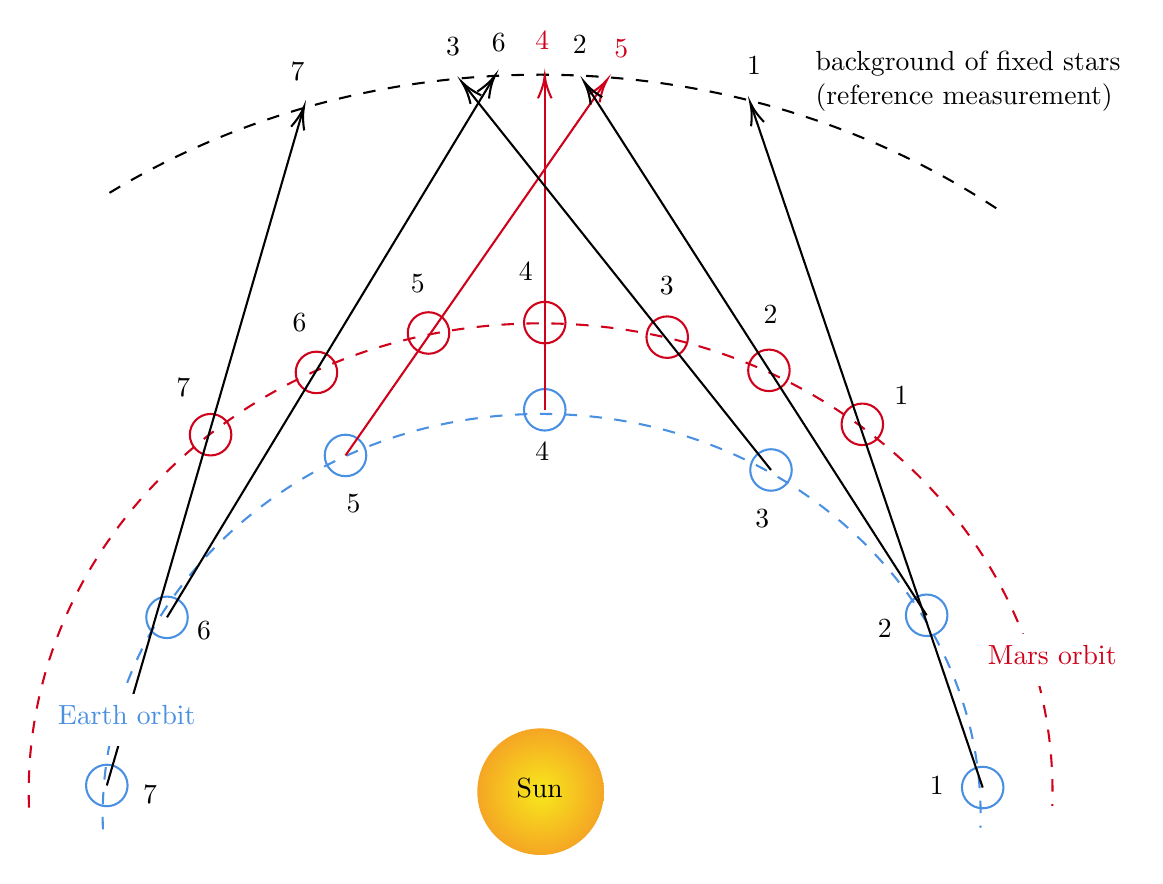
\begin{tikzpicture}[x=0.75pt,y=0.75pt,yscale=-1,xscale=1]
		%uncomment if require: \path (0,916); %set diagram left start at 0, and has height of 916

		% Gradient Info
		\tikzset {_74u8i7oz7/.code = {\pgfsetadditionalshadetransform{ \pgftransformshift{\pgfpoint{0 bp } { 0 bp }  }  \pgftransformscale{1 }  }}}
		\pgfdeclareradialshading{_yxuzzg3dj}{\pgfpoint{0bp}{0bp}}{rgb(0bp)=(0.97,0.91,0.11);
		rgb(0bp)=(0.97,0.91,0.11);
		rgb(25bp)=(0.96,0.65,0.14);
		rgb(400bp)=(0.96,0.65,0.14)}
				
		%Shape: Circle [id:dp5724433743250728] 
		\draw  [draw opacity=0][shading=_yxuzzg3dj,_74u8i7oz7] (274.5,390) .. controls (274.5,373.16) and (288.16,359.5) .. (305,359.5) .. controls (321.84,359.5) and (335.5,373.16) .. (335.5,390) .. controls (335.5,406.84) and (321.84,420.5) .. (305,420.5) .. controls (288.16,420.5) and (274.5,406.84) .. (274.5,390) -- cycle ;
		%Shape: Arc [id:dp8756995127052876] 
		\draw  [draw opacity=0][dash pattern={on 4.5pt off 4.5pt}] (94.12,408.11) .. controls (94.04,405.91) and (94,403.71) .. (94,401.5) .. controls (94,294.63) and (188.69,208) .. (305.5,208) .. controls (422.31,208) and (517,294.63) .. (517,401.5) .. controls (517,403.46) and (516.97,405.42) .. (516.9,407.37) -- (305.5,401.5) -- cycle ; \draw  [color={rgb, 255:red, 74; green, 144; blue, 226 }  ,draw opacity=1 ][dash pattern={on 4.5pt off 4.5pt}] (94.12,408.11) .. controls (94.04,405.91) and (94,403.71) .. (94,401.5) .. controls (94,294.63) and (188.69,208) .. (305.5,208) .. controls (422.31,208) and (517,294.63) .. (517,401.5) .. controls (517,403.46) and (516.97,405.42) .. (516.9,407.37) ;  
		%Shape: Arc [id:dp415420968471756] 
		\draw  [draw opacity=0][dash pattern={on 4.5pt off 4.5pt}] (58.51,397.7) .. controls (58.42,395.15) and (58.37,392.58) .. (58.37,390) .. controls (58.37,265.38) and (168.79,164.36) .. (305,164.36) .. controls (441.21,164.36) and (551.63,265.38) .. (551.63,390) .. controls (551.63,392.29) and (551.59,394.57) .. (551.52,396.84) -- (305,390) -- cycle ; \draw  [color={rgb, 255:red, 208; green, 2; blue, 27 }  ,draw opacity=1 ][dash pattern={on 4.5pt off 4.5pt}] (58.51,397.7) .. controls (58.42,395.15) and (58.37,392.58) .. (58.37,390) .. controls (58.37,265.38) and (168.79,164.36) .. (305,164.36) .. controls (441.21,164.36) and (551.63,265.38) .. (551.63,390) .. controls (551.63,392.29) and (551.59,394.57) .. (551.52,396.84) ;  
		%Shape: Arc [id:dp8058232207160336] 
		\draw  [draw opacity=0][dash pattern={on 4.5pt off 4.5pt}] (97.29,101.48) .. controls (156.88,65.5) and (228.27,44.56) .. (305,44.56) .. controls (388.19,44.56) and (465.1,69.17) .. (527.5,110.88) -- (305,390) -- cycle ; \draw  [color={rgb, 255:red, 0; green, 0; blue, 0 }  ,draw opacity=1 ][dash pattern={on 4.5pt off 4.5pt}] (97.29,101.48) .. controls (156.88,65.5) and (228.27,44.56) .. (305,44.56) .. controls (388.19,44.56) and (465.1,69.17) .. (527.5,110.88) ;  
		%Shape: Circle [id:dp5355907413157084] 
		\draw  [color={rgb, 255:red, 74; green, 144; blue, 226 }  ,draw opacity=1 ] (86,387) .. controls (86,381.48) and (90.48,377) .. (96,377) .. controls (101.52,377) and (106,381.48) .. (106,387) .. controls (106,392.52) and (101.52,397) .. (96,397) .. controls (90.48,397) and (86,392.52) .. (86,387) -- cycle ;
		%Shape: Circle [id:dp6693550347699555] 
		\draw  [color={rgb, 255:red, 74; green, 144; blue, 226 }  ,draw opacity=1 ] (115,306) .. controls (115,300.48) and (119.48,296) .. (125,296) .. controls (130.52,296) and (135,300.48) .. (135,306) .. controls (135,311.52) and (130.52,316) .. (125,316) .. controls (119.48,316) and (115,311.52) .. (115,306) -- cycle ;
		%Shape: Circle [id:dp47827615853326755] 
		\draw  [color={rgb, 255:red, 74; green, 144; blue, 226 }  ,draw opacity=1 ] (201,228) .. controls (201,222.48) and (205.48,218) .. (211,218) .. controls (216.52,218) and (221,222.48) .. (221,228) .. controls (221,233.52) and (216.52,238) .. (211,238) .. controls (205.48,238) and (201,233.52) .. (201,228) -- cycle ;
		%Shape: Circle [id:dp40720935252278956] 
		\draw  [color={rgb, 255:red, 74; green, 144; blue, 226 }  ,draw opacity=1 ] (297,206) .. controls (297,200.48) and (301.48,196) .. (307,196) .. controls (312.52,196) and (317,200.48) .. (317,206) .. controls (317,211.52) and (312.52,216) .. (307,216) .. controls (301.48,216) and (297,211.52) .. (297,206) -- cycle ;
		%Shape: Circle [id:dp4674525335015842] 
		\draw  [color={rgb, 255:red, 74; green, 144; blue, 226 }  ,draw opacity=1 ] (406,235) .. controls (406,229.48) and (410.48,225) .. (416,225) .. controls (421.52,225) and (426,229.48) .. (426,235) .. controls (426,240.52) and (421.52,245) .. (416,245) .. controls (410.48,245) and (406,240.52) .. (406,235) -- cycle ;
		%Shape: Circle [id:dp10873866048585445] 
		\draw  [color={rgb, 255:red, 74; green, 144; blue, 226 }  ,draw opacity=1 ] (481,305) .. controls (481,299.48) and (485.48,295) .. (491,295) .. controls (496.52,295) and (501,299.48) .. (501,305) .. controls (501,310.52) and (496.52,315) .. (491,315) .. controls (485.48,315) and (481,310.52) .. (481,305) -- cycle ;
		%Shape: Circle [id:dp21474665185641784] 
		\draw  [color={rgb, 255:red, 74; green, 144; blue, 226 }  ,draw opacity=1 ] (508,388) .. controls (508,382.48) and (512.48,378) .. (518,378) .. controls (523.52,378) and (528,382.48) .. (528,388) .. controls (528,393.52) and (523.52,398) .. (518,398) .. controls (512.48,398) and (508,393.52) .. (508,388) -- cycle ;
		%Shape: Circle [id:dp908549047123882] 
		\draw  [color={rgb, 255:red, 208; green, 2; blue, 27 }  ,draw opacity=1 ] (136,218) .. controls (136,212.48) and (140.48,208) .. (146,208) .. controls (151.52,208) and (156,212.48) .. (156,218) .. controls (156,223.52) and (151.52,228) .. (146,228) .. controls (140.48,228) and (136,223.52) .. (136,218) -- cycle ;
		%Shape: Circle [id:dp37394027075512337] 
		\draw  [color={rgb, 255:red, 208; green, 2; blue, 27 }  ,draw opacity=1 ] (187,188) .. controls (187,182.48) and (191.48,178) .. (197,178) .. controls (202.52,178) and (207,182.48) .. (207,188) .. controls (207,193.52) and (202.52,198) .. (197,198) .. controls (191.48,198) and (187,193.52) .. (187,188) -- cycle ;
		%Shape: Circle [id:dp6426663505355004] 
		\draw  [color={rgb, 255:red, 208; green, 2; blue, 27 }  ,draw opacity=1 ] (241,169) .. controls (241,163.48) and (245.48,159) .. (251,159) .. controls (256.52,159) and (261,163.48) .. (261,169) .. controls (261,174.52) and (256.52,179) .. (251,179) .. controls (245.48,179) and (241,174.52) .. (241,169) -- cycle ;
		%Shape: Circle [id:dp5210776018134717] 
		\draw  [color={rgb, 255:red, 208; green, 2; blue, 27 }  ,draw opacity=1 ] (297,164) .. controls (297,158.48) and (301.48,154) .. (307,154) .. controls (312.52,154) and (317,158.48) .. (317,164) .. controls (317,169.52) and (312.52,174) .. (307,174) .. controls (301.48,174) and (297,169.52) .. (297,164) -- cycle ;
		%Shape: Circle [id:dp8149819605601027] 
		\draw  [color={rgb, 255:red, 208; green, 2; blue, 27 }  ,draw opacity=1 ] (356,171) .. controls (356,165.48) and (360.48,161) .. (366,161) .. controls (371.52,161) and (376,165.48) .. (376,171) .. controls (376,176.52) and (371.52,181) .. (366,181) .. controls (360.48,181) and (356,176.52) .. (356,171) -- cycle ;
		%Shape: Circle [id:dp2695330079577125] 
		\draw  [color={rgb, 255:red, 208; green, 2; blue, 27 }  ,draw opacity=1 ] (405,187) .. controls (405,181.48) and (409.48,177) .. (415,177) .. controls (420.52,177) and (425,181.48) .. (425,187) .. controls (425,192.52) and (420.52,197) .. (415,197) .. controls (409.48,197) and (405,192.52) .. (405,187) -- cycle ;
		%Shape: Circle [id:dp14594923733230658] 
		\draw  [color={rgb, 255:red, 208; green, 2; blue, 27 }  ,draw opacity=1 ] (450,213) .. controls (450,207.48) and (454.48,203) .. (460,203) .. controls (465.52,203) and (470,207.48) .. (470,213) .. controls (470,218.52) and (465.52,223) .. (460,223) .. controls (454.48,223) and (450,218.52) .. (450,213) -- cycle ;
		%Straight Lines [id:da5034403453386942] 
		\draw    (96,387) -- (190.44,61.92) ;
		\draw [shift={(191,60)}, rotate = 106.2] [color={rgb, 255:red, 0; green, 0; blue, 0 }  ][line width=0.75]    (10.93,-3.29) .. controls (6.95,-1.4) and (3.31,-0.3) .. (0,0) .. controls (3.31,0.3) and (6.95,1.4) .. (10.93,3.29)   ;
		%Straight Lines [id:da03638541862475875] 
		\draw    (125,306) -- (281.96,46.71) ;
		\draw [shift={(283,45)}, rotate = 121.19] [color={rgb, 255:red, 0; green, 0; blue, 0 }  ][line width=0.75]    (10.93,-3.29) .. controls (6.95,-1.4) and (3.31,-0.3) .. (0,0) .. controls (3.31,0.3) and (6.95,1.4) .. (10.93,3.29)   ;
		%Straight Lines [id:da2920329885048476] 
		\draw [color={rgb, 255:red, 208; green, 2; blue, 27 }  ,draw opacity=1 ]   (211,228) -- (335.86,48.64) ;
		\draw [shift={(337,47)}, rotate = 124.84] [color={rgb, 255:red, 208; green, 2; blue, 27 }  ,draw opacity=1 ][line width=0.75]    (10.93,-3.29) .. controls (6.95,-1.4) and (3.31,-0.3) .. (0,0) .. controls (3.31,0.3) and (6.95,1.4) .. (10.93,3.29)   ;
		%Straight Lines [id:da4011479903660071] 
		\draw [color={rgb, 255:red, 208; green, 2; blue, 27 }  ,draw opacity=1 ]   (307,206) -- (307,47) ;
		\draw [shift={(307,45)}, rotate = 90] [color={rgb, 255:red, 208; green, 2; blue, 27 }  ,draw opacity=1 ][line width=0.75]    (10.93,-3.29) .. controls (6.95,-1.4) and (3.31,-0.3) .. (0,0) .. controls (3.31,0.3) and (6.95,1.4) .. (10.93,3.29)   ;
		%Straight Lines [id:da7897325170758853] 
		\draw    (416,235) -- (268.25,49.56) ;
		\draw [shift={(267,48)}, rotate = 51.45] [color={rgb, 255:red, 0; green, 0; blue, 0 }  ][line width=0.75]    (10.93,-3.29) .. controls (6.95,-1.4) and (3.31,-0.3) .. (0,0) .. controls (3.31,0.3) and (6.95,1.4) .. (10.93,3.29)   ;
		%Straight Lines [id:da7452917944256678] 
		\draw    (491,305) -- (327.08,49.68) ;
		\draw [shift={(326,48)}, rotate = 57.3] [color={rgb, 255:red, 0; green, 0; blue, 0 }  ][line width=0.75]    (10.93,-3.29) .. controls (6.95,-1.4) and (3.31,-0.3) .. (0,0) .. controls (3.31,0.3) and (6.95,1.4) .. (10.93,3.29)   ;
		%Straight Lines [id:da7584440179085579] 
		\draw    (518,388) -- (406.64,59.89) ;
		\draw [shift={(406,58)}, rotate = 71.25] [color={rgb, 255:red, 0; green, 0; blue, 0 }  ][line width=0.75]    (10.93,-3.29) .. controls (6.95,-1.4) and (3.31,-0.3) .. (0,0) .. controls (3.31,0.3) and (6.95,1.4) .. (10.93,3.29)   ;
		
		% Text Node
		\draw (292,382) node [anchor=north west][inner sep=0.75pt]   [align=left] {Sun};
		% Text Node
		\draw  [draw opacity=0][fill={rgb, 255:red, 255; green, 255; blue, 255 }  ,fill opacity=1 ]  (68,343) -- (145,343) -- (145,368) -- (68,368) -- cycle  ;
		\draw (71,347) node [anchor=north west][inner sep=0.75pt]  [color={rgb, 255:red, 74; green, 144; blue, 226 }  ,opacity=1 ] [align=left] {Earth orbit};
		% Text Node
		\draw  [draw opacity=0][fill={rgb, 255:red, 255; green, 255; blue, 255 }  ,fill opacity=1 ]  (516,314) -- (591,314) -- (591,339) -- (516,339) -- cycle  ;
		\draw (519,318) node [anchor=north west][inner sep=0.75pt]  [color={rgb, 255:red, 208; green, 2; blue, 27 }  ,opacity=1 ] [align=left] {Mars orbit};
		% Text Node
		\draw (112,385.4) node [anchor=north west][inner sep=0.75pt]    {$7$};
		% Text Node
		\draw (138,306.4) node [anchor=north west][inner sep=0.75pt]    {$6$};
		% Text Node
		\draw (210,245.4) node [anchor=north west][inner sep=0.75pt]    {$5$};
		% Text Node
		\draw (301,220.4) node [anchor=north west][inner sep=0.75pt]    {$4$};
		% Text Node
		\draw (407,252.4) node [anchor=north west][inner sep=0.75pt]    {$3$};
		% Text Node
		\draw (466,305.4) node [anchor=north west][inner sep=0.75pt]    {$2$};
		% Text Node
		\draw (491,381.4) node [anchor=north west][inner sep=0.75pt]    {$1$};
		% Text Node
		\draw (474,193.4) node [anchor=north west][inner sep=0.75pt]    {$1$};
		% Text Node
		\draw (411,154.4) node [anchor=north west][inner sep=0.75pt]    {$2$};
		% Text Node
		\draw (361,140.4) node [anchor=north west][inner sep=0.75pt]    {$3$};
		% Text Node
		\draw (293,133.4) node [anchor=north west][inner sep=0.75pt]    {$4$};
		% Text Node
		\draw (241,139.4) node [anchor=north west][inner sep=0.75pt]    {$5$};
		% Text Node
		\draw (184,158.4) node [anchor=north west][inner sep=0.75pt]    {$6$};
		% Text Node
		\draw (128,189.4) node [anchor=north west][inner sep=0.75pt]    {$7$};
		% Text Node
		\draw (183,37.4) node [anchor=north west][inner sep=0.75pt]    {$7$};
		% Text Node
		\draw (280,23.4) node [anchor=north west][inner sep=0.75pt]    {$6$};
		% Text Node
		\draw (258,25.4) node [anchor=north west][inner sep=0.75pt]    {$3$};
		% Text Node
		\draw (301,22.4) node [anchor=north west][inner sep=0.75pt]  [color={rgb, 255:red, 208; green, 2; blue, 27 }  ,opacity=1 ]  {$4$};
		% Text Node
		\draw (319,24.4) node [anchor=north west][inner sep=0.75pt]    {$2$};
		% Text Node
		\draw (339,26.4) node [anchor=north west][inner sep=0.75pt]  [color={rgb, 255:red, 208; green, 2; blue, 27 }  ,opacity=1 ]  {$5$};
		% Text Node
		\draw (403,34.4) node [anchor=north west][inner sep=0.75pt]    {$1$};
		% Text Node
		\draw (436,32) node [anchor=north west][inner sep=0.75pt]   [align=left] {background of fixed stars\\(reference measurement)};
		
		\end{tikzpicture}
		\vspace*{3mm}
		\caption[]{Figure to illustrate the choice of zero time}
	\end{figure}
	As the reader can check it in the figure above we see that the retrograde motion with respect to the fixed stars begins when the angle between the two planets is zero and it ends when the angle between the two planets pass through a maximum.

	Therefore, in the prior previous figure, we have:
	
	So to know the time between when the moment where the angle is zero between the two planets, reaches a maximum and decreases again, we simply need determine when occurs the sign of change in the previous function. To do this we just search when the derivative is zero:
	
	By applying the derivation rules seen in the section of Differential and Integral Calculus:
	
	Hence after simplification:
	
	We develop all this:
	
	and we simplify a first time:
	
	and second:
	
	and finally a third one:
	
	and after rearrangement:
	
	We simplify using trigonometric identities proved in the section  Trigonometry:
	
	The values of $t$ that satisfy this relation gives us the sign change we were looking for.

	If $t_0$ is the first value of $t$ that satisfies the equation, we have:
	
	The next value of $t$ will be such that:
	
	and therefore:
	
	If we introduce the rotation periods, we have:
	
	To come back to:
	
	it may be more convenient to write it in the traditional following form:
	
	So far, we have only do geometry. No law of gravitation intervened in the calculations. As the radius are unknown or little known (at least historically), we will use the Kepler's third law (periods law) that is for recall:
	
	where for recall $D$ is the semi-major axis of the orbit, and if it is circular, it becomes a simple radius. So we have:	
	
	Therefore:
	
	hence:
	
	A numerical application with for Mercury $T_1\cong 87.95$ [d] and for Earth $T_2\cong 365.25$ [d] lead to the value:
	
	Value that we have represented in the diagram below:
	\begin{figure}[H]
		\centering
		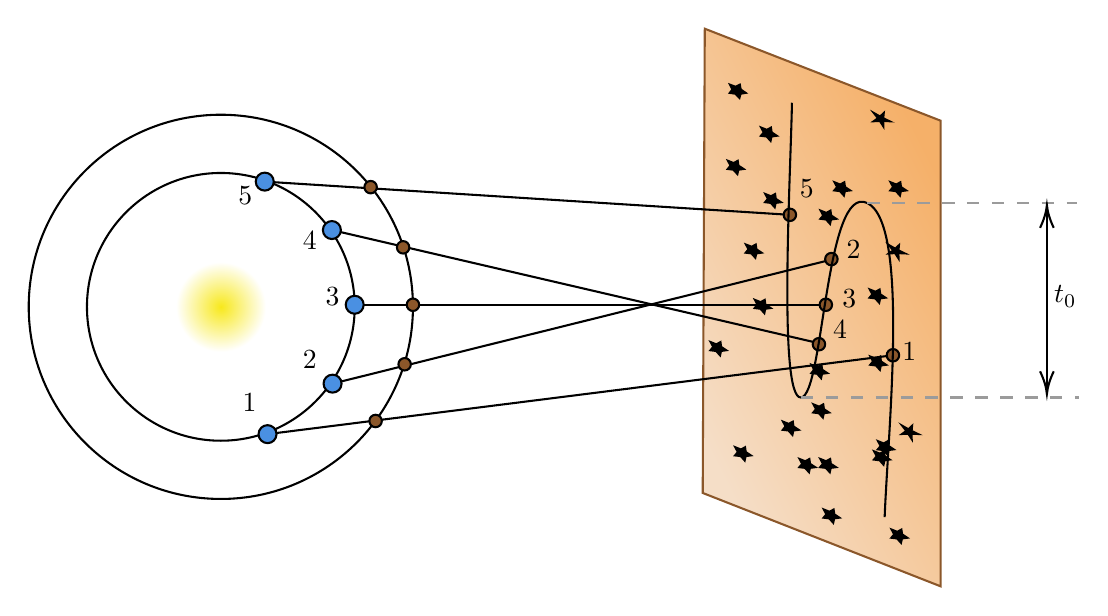
\begin{tikzpicture}[x=0.75pt,y=0.75pt,yscale=-1,xscale=1]
		%uncomment if require: \path (0,712); %set diagram left start at 0, and has height of 712

		% Gradient Info
		\tikzset {_ni6y6cjbw/.code = {\pgfsetadditionalshadetransform{ \pgftransformshift{\pgfpoint{0 bp } { 0 bp }  }  \pgftransformrotate{-310 }  \pgftransformscale{2 }  }}}
		\pgfdeclarehorizontalshading{_9s6tfjwzs}{150bp}{rgb(0bp)=(0.96,0.87,0.78);
		rgb(37.5bp)=(0.96,0.87,0.78);
		rgb(62.5bp)=(0.96,0.69,0.41);
		rgb(100bp)=(0.96,0.69,0.41)}
		
		% Gradient Info
		  
		\tikzset {_62kw9gixe/.code = {\pgfsetadditionalshadetransform{ \pgftransformshift{\pgfpoint{0 bp } { 0 bp }  }  \pgftransformscale{1.54 }  }}}
		\pgfdeclareradialshading{_72ri2gi5o}{\pgfpoint{0bp}{0bp}}{rgb(0bp)=(0.97,0.91,0.11);
		rgb(0bp)=(0.97,0.91,0.11);
		rgb(14.017857142857142bp)=(1,1,1);
		rgb(400bp)=(1,1,1)}
				
		%Shape: Polygon [id:ds8541353001148053] 
		\path  [shading=_9s6tfjwzs,_ni6y6cjbw] (371.17,48) -- (484.83,92.33) -- (484.83,212.33) -- (484.83,316.67) -- (370.17,271.67) -- cycle ; % for fading 
		 \draw  [color={rgb, 255:red, 139; green, 87; blue, 42 }  ,draw opacity=1 ] (371.17,48) -- (484.83,92.33) -- (484.83,212.33) -- (484.83,316.67) -- (370.17,271.67) -- cycle ; % for border 
		
		%Straight Lines [id:da07451099325639521] 
		\draw    (159.17,121.67) -- (412.17,137.67) ;
		%Straight Lines [id:da7804726949466878] 
		\draw    (191.5,145) -- (428.17,200) ;
		%Straight Lines [id:da519547051657969] 
		\draw    (202.5,181) -- (429.5,181) ;
		%Straight Lines [id:da19751671093574408] 
		\draw    (191.83,219) -- (433.17,159) ;
		%Straight Lines [id:da8590646002516045] 
		\draw    (160.5,243.33) -- (461.83,205.33) ;
		%Shape: Circle [id:dp2706888472046287] 
		\draw  [draw opacity=0][shading=_72ri2gi5o,_62kw9gixe] (113,182) .. controls (113,168.19) and (124.19,157) .. (138,157) .. controls (151.81,157) and (163,168.19) .. (163,182) .. controls (163,195.81) and (151.81,207) .. (138,207) .. controls (124.19,207) and (113,195.81) .. (113,182) -- cycle ;
		%Shape: Circle [id:dp01500239420106153] 
		\draw   (73.5,182) .. controls (73.5,146.38) and (102.38,117.5) .. (138,117.5) .. controls (173.62,117.5) and (202.5,146.38) .. (202.5,182) .. controls (202.5,217.62) and (173.62,246.5) .. (138,246.5) .. controls (102.38,246.5) and (73.5,217.62) .. (73.5,182) -- cycle ;
		%Shape: Circle [id:dp025367530788808823] 
		\draw   (45.44,182) .. controls (45.44,130.88) and (86.88,89.44) .. (138,89.44) .. controls (189.12,89.44) and (230.56,130.88) .. (230.56,182) .. controls (230.56,233.12) and (189.12,274.56) .. (138,274.56) .. controls (86.88,274.56) and (45.44,233.12) .. (45.44,182) -- cycle ;
		%Shape: Circle [id:dp7804672188082797] 
		\draw  [fill={rgb, 255:red, 74; green, 144; blue, 226 }  ,fill opacity=1 ] (154.83,121.67) .. controls (154.83,119.27) and (156.77,117.33) .. (159.17,117.33) .. controls (161.56,117.33) and (163.5,119.27) .. (163.5,121.67) .. controls (163.5,124.06) and (161.56,126) .. (159.17,126) .. controls (156.77,126) and (154.83,124.06) .. (154.83,121.67) -- cycle ;
		%Shape: Circle [id:dp28907899423216343] 
		\draw  [fill={rgb, 255:red, 74; green, 144; blue, 226 }  ,fill opacity=1 ] (187.17,145) .. controls (187.17,142.61) and (189.11,140.67) .. (191.5,140.67) .. controls (193.89,140.67) and (195.83,142.61) .. (195.83,145) .. controls (195.83,147.39) and (193.89,149.33) .. (191.5,149.33) .. controls (189.11,149.33) and (187.17,147.39) .. (187.17,145) -- cycle ;
		%Shape: Circle [id:dp766295540506932] 
		\draw  [fill={rgb, 255:red, 74; green, 144; blue, 226 }  ,fill opacity=1 ] (198.17,181) .. controls (198.17,178.61) and (200.11,176.67) .. (202.5,176.67) .. controls (204.89,176.67) and (206.83,178.61) .. (206.83,181) .. controls (206.83,183.39) and (204.89,185.33) .. (202.5,185.33) .. controls (200.11,185.33) and (198.17,183.39) .. (198.17,181) -- cycle ;
		%Shape: Circle [id:dp8140598497564899] 
		\draw  [fill={rgb, 255:red, 74; green, 144; blue, 226 }  ,fill opacity=1 ] (187.5,219) .. controls (187.5,216.61) and (189.44,214.67) .. (191.83,214.67) .. controls (194.23,214.67) and (196.17,216.61) .. (196.17,219) .. controls (196.17,221.39) and (194.23,223.33) .. (191.83,223.33) .. controls (189.44,223.33) and (187.5,221.39) .. (187.5,219) -- cycle ;
		%Shape: Circle [id:dp21080342593265433] 
		\draw  [fill={rgb, 255:red, 74; green, 144; blue, 226 }  ,fill opacity=1 ] (156.17,243.33) .. controls (156.17,240.94) and (158.11,239) .. (160.5,239) .. controls (162.89,239) and (164.83,240.94) .. (164.83,243.33) .. controls (164.83,245.73) and (162.89,247.67) .. (160.5,247.67) .. controls (158.11,247.67) and (156.17,245.73) .. (156.17,243.33) -- cycle ;
		%Shape: Circle [id:dp9548438696764499] 
		\draw  [fill={rgb, 255:red, 139; green, 87; blue, 42 }  ,fill opacity=1 ] (207.17,124.33) .. controls (207.17,122.68) and (208.51,121.33) .. (210.17,121.33) .. controls (211.82,121.33) and (213.17,122.68) .. (213.17,124.33) .. controls (213.17,125.99) and (211.82,127.33) .. (210.17,127.33) .. controls (208.51,127.33) and (207.17,125.99) .. (207.17,124.33) -- cycle ;
		%Shape: Circle [id:dp888012370144196] 
		\draw  [fill={rgb, 255:red, 139; green, 87; blue, 42 }  ,fill opacity=1 ] (222.83,153.33) .. controls (222.83,151.68) and (224.18,150.33) .. (225.83,150.33) .. controls (227.49,150.33) and (228.83,151.68) .. (228.83,153.33) .. controls (228.83,154.99) and (227.49,156.33) .. (225.83,156.33) .. controls (224.18,156.33) and (222.83,154.99) .. (222.83,153.33) -- cycle ;
		%Shape: Circle [id:dp4285995465584147] 
		\draw  [fill={rgb, 255:red, 139; green, 87; blue, 42 }  ,fill opacity=1 ] (227.56,181) .. controls (227.56,179.34) and (228.91,178) .. (230.56,178) .. controls (232.22,178) and (233.56,179.34) .. (233.56,181) .. controls (233.56,182.66) and (232.22,184) .. (230.56,184) .. controls (228.91,184) and (227.56,182.66) .. (227.56,181) -- cycle ;
		%Shape: Circle [id:dp6048183661988833] 
		\draw  [fill={rgb, 255:red, 139; green, 87; blue, 42 }  ,fill opacity=1 ] (223.56,209.67) .. controls (223.56,208.01) and (224.91,206.67) .. (226.56,206.67) .. controls (228.22,206.67) and (229.56,208.01) .. (229.56,209.67) .. controls (229.56,211.32) and (228.22,212.67) .. (226.56,212.67) .. controls (224.91,212.67) and (223.56,211.32) .. (223.56,209.67) -- cycle ;
		%Shape: Circle [id:dp8181982278752085] 
		\draw  [fill={rgb, 255:red, 139; green, 87; blue, 42 }  ,fill opacity=1 ] (209.56,237) .. controls (209.56,235.34) and (210.91,234) .. (212.56,234) .. controls (214.22,234) and (215.56,235.34) .. (215.56,237) .. controls (215.56,238.66) and (214.22,240) .. (212.56,240) .. controls (210.91,240) and (209.56,238.66) .. (209.56,237) -- cycle ;
		%Shape: Circle [id:dp10123219902889713] 
		\draw  [fill={rgb, 255:red, 139; green, 87; blue, 42 }  ,fill opacity=1 ] (409.17,137.67) .. controls (409.17,136.01) and (410.51,134.67) .. (412.17,134.67) .. controls (413.82,134.67) and (415.17,136.01) .. (415.17,137.67) .. controls (415.17,139.32) and (413.82,140.67) .. (412.17,140.67) .. controls (410.51,140.67) and (409.17,139.32) .. (409.17,137.67) -- cycle ;
		%Shape: Circle [id:dp7172832009675363] 
		\draw  [fill={rgb, 255:red, 139; green, 87; blue, 42 }  ,fill opacity=1 ] (429.17,159) .. controls (429.17,157.34) and (430.51,156) .. (432.17,156) .. controls (433.82,156) and (435.17,157.34) .. (435.17,159) .. controls (435.17,160.66) and (433.82,162) .. (432.17,162) .. controls (430.51,162) and (429.17,160.66) .. (429.17,159) -- cycle ;
		%Shape: Circle [id:dp010644652182668635] 
		\draw  [fill={rgb, 255:red, 139; green, 87; blue, 42 }  ,fill opacity=1 ] (426.5,181) .. controls (426.5,179.34) and (427.84,178) .. (429.5,178) .. controls (431.16,178) and (432.5,179.34) .. (432.5,181) .. controls (432.5,182.66) and (431.16,184) .. (429.5,184) .. controls (427.84,184) and (426.5,182.66) .. (426.5,181) -- cycle ;
		%Shape: Circle [id:dp058103181928748526] 
		\draw  [fill={rgb, 255:red, 139; green, 87; blue, 42 }  ,fill opacity=1 ] (423.17,200) .. controls (423.17,198.34) and (424.51,197) .. (426.17,197) .. controls (427.82,197) and (429.17,198.34) .. (429.17,200) .. controls (429.17,201.66) and (427.82,203) .. (426.17,203) .. controls (424.51,203) and (423.17,201.66) .. (423.17,200) -- cycle ;
		%Shape: Circle [id:dp6478836419654275] 
		\draw  [fill={rgb, 255:red, 139; green, 87; blue, 42 }  ,fill opacity=1 ] (458.83,205.33) .. controls (458.83,203.68) and (460.18,202.33) .. (461.83,202.33) .. controls (463.49,202.33) and (464.83,203.68) .. (464.83,205.33) .. controls (464.83,206.99) and (463.49,208.33) .. (461.83,208.33) .. controls (460.18,208.33) and (458.83,206.99) .. (458.83,205.33) -- cycle ;
		%Curve Lines [id:da36287602823884346] 
		\draw    (413.17,83.67) .. controls (412.5,119) and (406.5,226.33) .. (417.5,225.67) .. controls (428.5,225) and (429.17,122) .. (449.5,132) .. controls (469.83,142) and (459.5,240.33) .. (457.83,283.33) ;
		%Shape: Star [id:dp866386479336466] 
		\draw  [fill={rgb, 255:red, 0; green, 0; blue, 0 }  ,fill opacity=1 ] (387.86,81.33) -- (388.4,79.32) -- (390.82,78.91) -- (388.46,77.27) -- (388.04,75) -- (386.04,76) -- (383.37,75) -- (384.49,77.27) -- (383.25,78.91) -- (385.95,79.32) -- cycle ;
		%Shape: Star [id:dp015393464208243834] 
		\draw  [fill={rgb, 255:red, 0; green, 0; blue, 0 }  ,fill opacity=1 ] (457.19,95) -- (457.1,92.44) -- (460.15,92.58) -- (457.14,91.14) -- (457.38,88.67) -- (455.6,90.33) -- (452.7,88.67) -- (454.62,91.14) -- (452.58,92.58) -- (455.54,92.44) -- cycle ;
		%Shape: Star [id:dp8086191372267226] 
		\draw  [fill={rgb, 255:red, 0; green, 0; blue, 0 }  ,fill opacity=1 ] (402.86,102) -- (403.32,99.92) -- (405.82,99.58) -- (403.37,97.96) -- (403.04,95.67) -- (401.07,96.75) -- (398.37,95.67) -- (399.59,97.96) -- (398.25,99.58) -- (400.98,99.92) -- cycle ;
		%Shape: Star [id:dp2713126161044501] 
		\draw  [fill={rgb, 255:red, 0; green, 0; blue, 0 }  ,fill opacity=1 ] (386.86,118) -- (387.32,115.92) -- (389.82,115.58) -- (387.37,113.96) -- (387.04,111.67) -- (385.07,112.75) -- (382.37,111.67) -- (383.59,113.96) -- (382.25,115.58) -- (384.98,115.92) -- cycle ;
		%Shape: Star [id:dp23138514457294868] 
		\draw  [fill={rgb, 255:red, 0; green, 0; blue, 0 }  ,fill opacity=1 ] (404.86,134) -- (405.32,131.92) -- (407.82,131.58) -- (405.37,129.96) -- (405.04,127.67) -- (403.07,128.75) -- (400.37,127.67) -- (401.59,129.96) -- (400.25,131.58) -- (402.98,131.92) -- cycle ;
		%Shape: Star [id:dp501829984169061] 
		\draw  [fill={rgb, 255:red, 0; green, 0; blue, 0 }  ,fill opacity=1 ] (431.52,142) -- (431.98,139.92) -- (434.48,139.58) -- (432.04,137.96) -- (431.71,135.67) -- (429.74,136.75) -- (427.03,135.67) -- (428.26,137.96) -- (426.92,139.58) -- (429.65,139.92) -- cycle ;
		%Shape: Star [id:dp005626227320733257] 
		\draw  [fill={rgb, 255:red, 0; green, 0; blue, 0 }  ,fill opacity=1 ] (438.19,128.33) -- (438.65,126.25) -- (441.15,125.91) -- (438.71,124.29) -- (438.38,122) -- (436.41,123.08) -- (433.7,122) -- (434.92,124.29) -- (433.58,125.91) -- (436.31,126.25) -- cycle ;
		%Shape: Star [id:dp4072778228163567] 
		\draw  [fill={rgb, 255:red, 0; green, 0; blue, 0 }  ,fill opacity=1 ] (465.19,128.33) -- (465.65,126.25) -- (468.15,125.91) -- (465.71,124.29) -- (465.38,122) -- (463.41,123.08) -- (460.7,122) -- (461.92,124.29) -- (460.58,125.91) -- (463.31,126.25) -- cycle ;
		%Shape: Star [id:dp6472114222537886] 
		\draw  [fill={rgb, 255:red, 0; green, 0; blue, 0 }  ,fill opacity=1 ] (464.52,158.67) -- (464.43,156.11) -- (467.48,156.25) -- (464.47,154.81) -- (464.71,152.34) -- (462.94,154) -- (460.03,152.34) -- (461.95,154.81) -- (459.92,156.25) -- (462.87,156.11) -- cycle ;
		%Shape: Star [id:dp6998498624265717] 
		\draw  [fill={rgb, 255:red, 0; green, 0; blue, 0 }  ,fill opacity=1 ] (455.19,180) -- (455.65,177.92) -- (458.15,177.58) -- (455.71,175.96) -- (455.38,173.67) -- (453.41,174.75) -- (450.7,173.67) -- (451.92,175.96) -- (450.58,177.58) -- (453.31,177.92) -- cycle ;
		%Shape: Star [id:dp5337030557289695] 
		\draw  [fill={rgb, 255:red, 0; green, 0; blue, 0 }  ,fill opacity=1 ] (399.86,185) -- (400.32,182.92) -- (402.82,182.58) -- (400.37,180.96) -- (400.04,178.67) -- (398.07,179.75) -- (395.37,178.67) -- (396.59,180.96) -- (395.25,182.58) -- (397.98,182.92) -- cycle ;
		%Shape: Star [id:dp40021992461469025] 
		\draw  [fill={rgb, 255:red, 0; green, 0; blue, 0 }  ,fill opacity=1 ] (395.52,158.33) -- (395.98,156.25) -- (398.48,155.91) -- (396.04,154.29) -- (395.71,152) -- (393.74,153.08) -- (391.03,152) -- (392.26,154.29) -- (390.92,155.91) -- (393.65,156.25) -- cycle ;
		%Shape: Star [id:dp41042001861475685] 
		\draw  [fill={rgb, 255:red, 0; green, 0; blue, 0 }  ,fill opacity=1 ] (378.52,205.33) -- (378.98,203.25) -- (381.48,202.91) -- (379.04,201.29) -- (378.71,199) -- (376.74,200.08) -- (374.03,199) -- (375.26,201.29) -- (373.92,202.91) -- (376.65,203.25) -- cycle ;
		%Shape: Star [id:dp5814490159128156] 
		\draw  [fill={rgb, 255:red, 0; green, 0; blue, 0 }  ,fill opacity=1 ] (427.19,216.33) -- (427.65,214.25) -- (430.15,213.91) -- (427.71,212.29) -- (427.38,210) -- (425.41,211.08) -- (422.7,210) -- (423.92,212.29) -- (422.58,213.91) -- (425.31,214.25) -- cycle ;
		%Shape: Star [id:dp7241103328832841] 
		\draw  [fill={rgb, 255:red, 0; green, 0; blue, 0 }  ,fill opacity=1 ] (455.52,212.33) -- (455.98,210.25) -- (458.48,209.91) -- (456.04,208.29) -- (455.71,206) -- (453.74,207.08) -- (451.03,206) -- (452.26,208.29) -- (450.92,209.91) -- (453.65,210.25) -- cycle ;
		%Shape: Star [id:dp19471113347685565] 
		\draw  [fill={rgb, 255:red, 0; green, 0; blue, 0 }  ,fill opacity=1 ] (470.86,245.67) -- (470.77,243.11) -- (473.82,243.25) -- (470.81,241.81) -- (471.04,239.34) -- (469.27,241) -- (466.37,239.34) -- (468.28,241.81) -- (466.25,243.25) -- (469.21,243.11) -- cycle ;
		%Shape: Star [id:dp8097084471352554] 
		\draw  [fill={rgb, 255:red, 0; green, 0; blue, 0 }  ,fill opacity=1 ] (459.16,253.08) -- (459.62,251) -- (462.12,250.66) -- (459.68,249.04) -- (459.35,246.75) -- (457.38,247.83) -- (454.67,246.75) -- (455.9,249.04) -- (454.56,250.66) -- (457.28,251) -- cycle ;
		%Shape: Star [id:dp7163482706481454] 
		\draw  [fill={rgb, 255:red, 0; green, 0; blue, 0 }  ,fill opacity=1 ] (457.28,258) -- (457.74,255.91) -- (460.24,255.58) -- (457.8,253.96) -- (457.47,251.67) -- (455.5,252.75) -- (452.79,251.67) -- (454.02,253.96) -- (452.68,255.58) -- (455.41,255.91) -- cycle ;
		%Shape: Star [id:dp39472478937111166] 
		\draw  [fill={rgb, 255:red, 0; green, 0; blue, 0 }  ,fill opacity=1 ] (465.71,295.66) -- (466.17,293.58) -- (468.67,293.25) -- (466.23,291.62) -- (465.89,289.33) -- (463.92,290.41) -- (461.22,289.33) -- (462.44,291.62) -- (461.1,293.25) -- (463.83,293.58) -- cycle ;
		%Shape: Star [id:dp9115061565087199] 
		\draw  [fill={rgb, 255:red, 0; green, 0; blue, 0 }  ,fill opacity=1 ] (433.04,286) -- (433.5,283.91) -- (436,283.58) -- (433.56,281.96) -- (433.23,279.67) -- (431.26,280.75) -- (428.55,279.67) -- (429.78,281.96) -- (428.44,283.58) -- (431.16,283.91) -- cycle ;
		%Shape: Star [id:dp3169299400425727] 
		\draw  [fill={rgb, 255:red, 0; green, 0; blue, 0 }  ,fill opacity=1 ] (431.38,261.66) -- (431.84,259.58) -- (434.34,259.25) -- (431.89,257.62) -- (431.56,255.33) -- (429.59,256.41) -- (426.89,255.33) -- (428.11,257.62) -- (426.77,259.25) -- (429.5,259.58) -- cycle ;
		%Shape: Star [id:dp2880812091604008] 
		\draw  [fill={rgb, 255:red, 0; green, 0; blue, 0 }  ,fill opacity=1 ] (421.38,261.66) -- (421.84,259.58) -- (424.34,259.25) -- (421.89,257.62) -- (421.56,255.33) -- (419.59,256.41) -- (416.89,255.33) -- (418.11,257.62) -- (416.77,259.25) -- (419.5,259.58) -- cycle ;
		%Shape: Star [id:dp8825750561297709] 
		\draw  [fill={rgb, 255:red, 0; green, 0; blue, 0 }  ,fill opacity=1 ] (428.04,235.33) -- (428.5,233.25) -- (431,232.91) -- (428.56,231.29) -- (428.23,229) -- (426.26,230.08) -- (423.55,229) -- (424.78,231.29) -- (423.44,232.91) -- (426.16,233.25) -- cycle ;
		%Shape: Star [id:dp2449171351888122] 
		\draw  [fill={rgb, 255:red, 0; green, 0; blue, 0 }  ,fill opacity=1 ] (413.38,243.66) -- (413.84,241.58) -- (416.34,241.25) -- (413.89,239.62) -- (413.56,237.33) -- (411.59,238.41) -- (408.89,237.33) -- (410.11,239.62) -- (408.77,241.25) -- (411.5,241.58) -- cycle ;
		%Shape: Star [id:dp5413168509265052] 
		\draw  [fill={rgb, 255:red, 0; green, 0; blue, 0 }  ,fill opacity=1 ] (390.38,256) -- (390.84,253.91) -- (393.34,253.58) -- (390.89,251.96) -- (390.56,249.67) -- (388.59,250.75) -- (385.89,249.67) -- (387.11,251.96) -- (385.77,253.58) -- (388.5,253.91) -- cycle ;
		%Straight Lines [id:da7434473487556048] 
		\draw [color={rgb, 255:red, 155; green, 155; blue, 155 }  ,draw opacity=1 ] [dash pattern={on 4.5pt off 4.5pt}]  (449.5,132) -- (550.5,132) ;
		%Straight Lines [id:da176154486458016] 
		\draw [color={rgb, 255:red, 155; green, 155; blue, 155 }  ,draw opacity=1 ] [dash pattern={on 4.5pt off 4.5pt}]  (417.5,225.67) -- (551.5,225.67) ;
		%Straight Lines [id:da21123388550873923] 
		\draw    (536,135) -- (536,222) ;
		\draw [shift={(536,224)}, rotate = 270] [color={rgb, 255:red, 0; green, 0; blue, 0 }  ][line width=0.75]    (10.93,-3.29) .. controls (6.95,-1.4) and (3.31,-0.3) .. (0,0) .. controls (3.31,0.3) and (6.95,1.4) .. (10.93,3.29)   ;
		\draw [shift={(536,133)}, rotate = 90] [color={rgb, 255:red, 0; green, 0; blue, 0 }  ][line width=0.75]    (10.93,-3.29) .. controls (6.95,-1.4) and (3.31,-0.3) .. (0,0) .. controls (3.31,0.3) and (6.95,1.4) .. (10.93,3.29)   ;
		
		% Text Node
		\draw (145,122.4) node [anchor=north west][inner sep=0.75pt]    {$5$};
		% Text Node
		\draw (176,144.4) node [anchor=north west][inner sep=0.75pt]    {$4$};
		% Text Node
		\draw (187,171.4) node [anchor=north west][inner sep=0.75pt]    {$3$};
		% Text Node
		\draw (176,201.4) node [anchor=north west][inner sep=0.75pt]    {$2$};
		% Text Node
		\draw (147,222.4) node [anchor=north west][inner sep=0.75pt]    {$1$};
		% Text Node
		\draw (464.83,197.73) node [anchor=north west][inner sep=0.75pt]    {$1$};
		% Text Node
		\draw (438,148.4) node [anchor=north west][inner sep=0.75pt]    {$2$};
		% Text Node
		\draw (436,172.4) node [anchor=north west][inner sep=0.75pt]    {$3$};
		% Text Node
		\draw (431.5,187.4) node [anchor=north west][inner sep=0.75pt]    {$4$};
		% Text Node
		\draw (415.5,119.4) node [anchor=north west][inner sep=0.75pt]    {$5$};
		% Text Node
		\draw (538,170.4) node [anchor=north west][inner sep=0.75pt]    {$t_{0}$};
		
		\end{tikzpicture}
	\end{figure}
	and therefore:
	\begin{figure}[H]
		\centering
		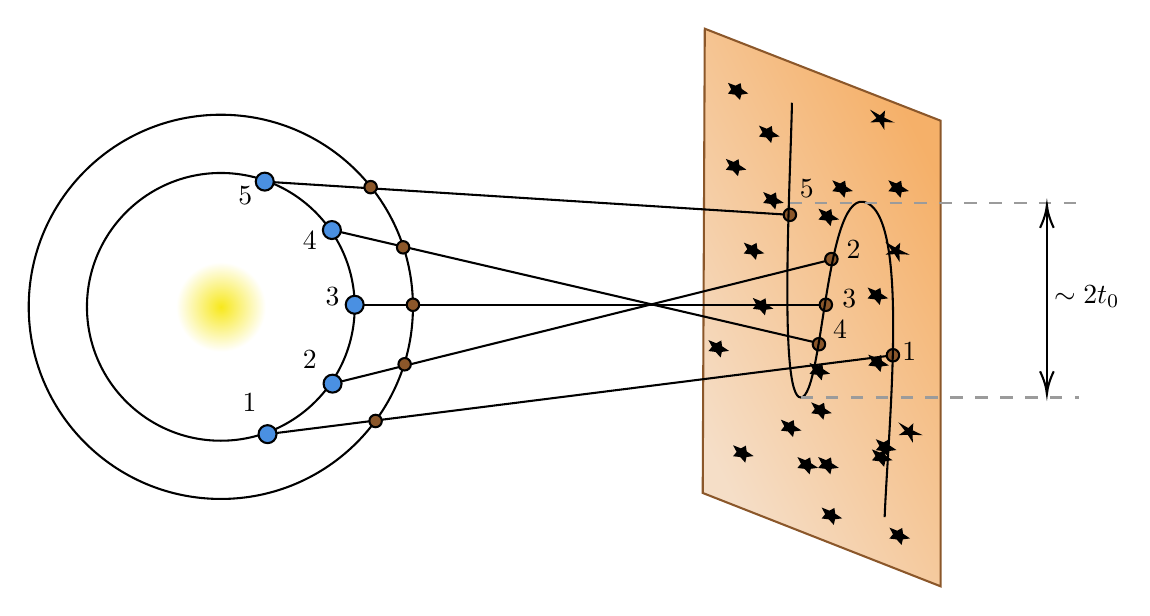
\begin{tikzpicture}[x=0.75pt,y=0.75pt,yscale=-1,xscale=1]
		%uncomment if require: \path (0,712); %set diagram left start at 0, and has height of 712

		% Gradient Info
		\tikzset {_lxru5ma0q/.code = {\pgfsetadditionalshadetransform{ \pgftransformshift{\pgfpoint{0 bp } { 0 bp }  }  \pgftransformrotate{-310 }  \pgftransformscale{2 }  }}}
		\pgfdeclarehorizontalshading{_i3t6lt59p}{150bp}{rgb(0bp)=(0.96,0.87,0.78);
		rgb(37.5bp)=(0.96,0.87,0.78);
		rgb(62.5bp)=(0.96,0.69,0.41);
		rgb(100bp)=(0.96,0.69,0.41)}
		
		% Gradient Info
		  
		\tikzset {_3ovxum8zq/.code = {\pgfsetadditionalshadetransform{ \pgftransformshift{\pgfpoint{0 bp } { 0 bp }  }  \pgftransformscale{1.54 }  }}}
		\pgfdeclareradialshading{_sezpll4y3}{\pgfpoint{0bp}{0bp}}{rgb(0bp)=(0.97,0.91,0.11);
		rgb(0bp)=(0.97,0.91,0.11);
		rgb(14.017857142857142bp)=(1,1,1);
		rgb(400bp)=(1,1,1)}
				
		%Shape: Polygon [id:ds8541353001148053] 
		\path  [shading=_i3t6lt59p,_lxru5ma0q] (371.17,48) -- (484.83,92.33) -- (484.83,212.33) -- (484.83,316.67) -- (370.17,271.67) -- cycle ; % for fading 
		 \draw  [color={rgb, 255:red, 139; green, 87; blue, 42 }  ,draw opacity=1 ] (371.17,48) -- (484.83,92.33) -- (484.83,212.33) -- (484.83,316.67) -- (370.17,271.67) -- cycle ; % for border 
		
		%Straight Lines [id:da07451099325639521] 
		\draw    (159.17,121.67) -- (412.17,137.67) ;
		%Straight Lines [id:da7804726949466878] 
		\draw    (191.5,145) -- (428.17,200) ;
		%Straight Lines [id:da519547051657969] 
		\draw    (202.5,181) -- (429.5,181) ;
		%Straight Lines [id:da19751671093574408] 
		\draw    (191.83,219) -- (433.17,159) ;
		%Straight Lines [id:da8590646002516045] 
		\draw    (160.5,243.33) -- (461.83,205.33) ;
		%Shape: Circle [id:dp2706888472046287] 
		\draw  [draw opacity=0][shading=_sezpll4y3,_3ovxum8zq] (113,182) .. controls (113,168.19) and (124.19,157) .. (138,157) .. controls (151.81,157) and (163,168.19) .. (163,182) .. controls (163,195.81) and (151.81,207) .. (138,207) .. controls (124.19,207) and (113,195.81) .. (113,182) -- cycle ;
		%Shape: Circle [id:dp01500239420106153] 
		\draw   (73.5,182) .. controls (73.5,146.38) and (102.38,117.5) .. (138,117.5) .. controls (173.62,117.5) and (202.5,146.38) .. (202.5,182) .. controls (202.5,217.62) and (173.62,246.5) .. (138,246.5) .. controls (102.38,246.5) and (73.5,217.62) .. (73.5,182) -- cycle ;
		%Shape: Circle [id:dp025367530788808823] 
		\draw   (45.44,182) .. controls (45.44,130.88) and (86.88,89.44) .. (138,89.44) .. controls (189.12,89.44) and (230.56,130.88) .. (230.56,182) .. controls (230.56,233.12) and (189.12,274.56) .. (138,274.56) .. controls (86.88,274.56) and (45.44,233.12) .. (45.44,182) -- cycle ;
		%Shape: Circle [id:dp7804672188082797] 
		\draw  [fill={rgb, 255:red, 74; green, 144; blue, 226 }  ,fill opacity=1 ] (154.83,121.67) .. controls (154.83,119.27) and (156.77,117.33) .. (159.17,117.33) .. controls (161.56,117.33) and (163.5,119.27) .. (163.5,121.67) .. controls (163.5,124.06) and (161.56,126) .. (159.17,126) .. controls (156.77,126) and (154.83,124.06) .. (154.83,121.67) -- cycle ;
		%Shape: Circle [id:dp28907899423216343] 
		\draw  [fill={rgb, 255:red, 74; green, 144; blue, 226 }  ,fill opacity=1 ] (187.17,145) .. controls (187.17,142.61) and (189.11,140.67) .. (191.5,140.67) .. controls (193.89,140.67) and (195.83,142.61) .. (195.83,145) .. controls (195.83,147.39) and (193.89,149.33) .. (191.5,149.33) .. controls (189.11,149.33) and (187.17,147.39) .. (187.17,145) -- cycle ;
		%Shape: Circle [id:dp766295540506932] 
		\draw  [fill={rgb, 255:red, 74; green, 144; blue, 226 }  ,fill opacity=1 ] (198.17,181) .. controls (198.17,178.61) and (200.11,176.67) .. (202.5,176.67) .. controls (204.89,176.67) and (206.83,178.61) .. (206.83,181) .. controls (206.83,183.39) and (204.89,185.33) .. (202.5,185.33) .. controls (200.11,185.33) and (198.17,183.39) .. (198.17,181) -- cycle ;
		%Shape: Circle [id:dp8140598497564899] 
		\draw  [fill={rgb, 255:red, 74; green, 144; blue, 226 }  ,fill opacity=1 ] (187.5,219) .. controls (187.5,216.61) and (189.44,214.67) .. (191.83,214.67) .. controls (194.23,214.67) and (196.17,216.61) .. (196.17,219) .. controls (196.17,221.39) and (194.23,223.33) .. (191.83,223.33) .. controls (189.44,223.33) and (187.5,221.39) .. (187.5,219) -- cycle ;
		%Shape: Circle [id:dp21080342593265433] 
		\draw  [fill={rgb, 255:red, 74; green, 144; blue, 226 }  ,fill opacity=1 ] (156.17,243.33) .. controls (156.17,240.94) and (158.11,239) .. (160.5,239) .. controls (162.89,239) and (164.83,240.94) .. (164.83,243.33) .. controls (164.83,245.73) and (162.89,247.67) .. (160.5,247.67) .. controls (158.11,247.67) and (156.17,245.73) .. (156.17,243.33) -- cycle ;
		%Shape: Circle [id:dp9548438696764499] 
		\draw  [fill={rgb, 255:red, 139; green, 87; blue, 42 }  ,fill opacity=1 ] (207.17,124.33) .. controls (207.17,122.68) and (208.51,121.33) .. (210.17,121.33) .. controls (211.82,121.33) and (213.17,122.68) .. (213.17,124.33) .. controls (213.17,125.99) and (211.82,127.33) .. (210.17,127.33) .. controls (208.51,127.33) and (207.17,125.99) .. (207.17,124.33) -- cycle ;
		%Shape: Circle [id:dp888012370144196] 
		\draw  [fill={rgb, 255:red, 139; green, 87; blue, 42 }  ,fill opacity=1 ] (222.83,153.33) .. controls (222.83,151.68) and (224.18,150.33) .. (225.83,150.33) .. controls (227.49,150.33) and (228.83,151.68) .. (228.83,153.33) .. controls (228.83,154.99) and (227.49,156.33) .. (225.83,156.33) .. controls (224.18,156.33) and (222.83,154.99) .. (222.83,153.33) -- cycle ;
		%Shape: Circle [id:dp4285995465584147] 
		\draw  [fill={rgb, 255:red, 139; green, 87; blue, 42 }  ,fill opacity=1 ] (227.56,181) .. controls (227.56,179.34) and (228.91,178) .. (230.56,178) .. controls (232.22,178) and (233.56,179.34) .. (233.56,181) .. controls (233.56,182.66) and (232.22,184) .. (230.56,184) .. controls (228.91,184) and (227.56,182.66) .. (227.56,181) -- cycle ;
		%Shape: Circle [id:dp6048183661988833] 
		\draw  [fill={rgb, 255:red, 139; green, 87; blue, 42 }  ,fill opacity=1 ] (223.56,209.67) .. controls (223.56,208.01) and (224.91,206.67) .. (226.56,206.67) .. controls (228.22,206.67) and (229.56,208.01) .. (229.56,209.67) .. controls (229.56,211.32) and (228.22,212.67) .. (226.56,212.67) .. controls (224.91,212.67) and (223.56,211.32) .. (223.56,209.67) -- cycle ;
		%Shape: Circle [id:dp8181982278752085] 
		\draw  [fill={rgb, 255:red, 139; green, 87; blue, 42 }  ,fill opacity=1 ] (209.56,237) .. controls (209.56,235.34) and (210.91,234) .. (212.56,234) .. controls (214.22,234) and (215.56,235.34) .. (215.56,237) .. controls (215.56,238.66) and (214.22,240) .. (212.56,240) .. controls (210.91,240) and (209.56,238.66) .. (209.56,237) -- cycle ;
		%Shape: Circle [id:dp10123219902889713] 
		\draw  [fill={rgb, 255:red, 139; green, 87; blue, 42 }  ,fill opacity=1 ] (409.17,137.67) .. controls (409.17,136.01) and (410.51,134.67) .. (412.17,134.67) .. controls (413.82,134.67) and (415.17,136.01) .. (415.17,137.67) .. controls (415.17,139.32) and (413.82,140.67) .. (412.17,140.67) .. controls (410.51,140.67) and (409.17,139.32) .. (409.17,137.67) -- cycle ;
		%Shape: Circle [id:dp7172832009675363] 
		\draw  [fill={rgb, 255:red, 139; green, 87; blue, 42 }  ,fill opacity=1 ] (429.17,159) .. controls (429.17,157.34) and (430.51,156) .. (432.17,156) .. controls (433.82,156) and (435.17,157.34) .. (435.17,159) .. controls (435.17,160.66) and (433.82,162) .. (432.17,162) .. controls (430.51,162) and (429.17,160.66) .. (429.17,159) -- cycle ;
		%Shape: Circle [id:dp010644652182668635] 
		\draw  [fill={rgb, 255:red, 139; green, 87; blue, 42 }  ,fill opacity=1 ] (426.5,181) .. controls (426.5,179.34) and (427.84,178) .. (429.5,178) .. controls (431.16,178) and (432.5,179.34) .. (432.5,181) .. controls (432.5,182.66) and (431.16,184) .. (429.5,184) .. controls (427.84,184) and (426.5,182.66) .. (426.5,181) -- cycle ;
		%Shape: Circle [id:dp058103181928748526] 
		\draw  [fill={rgb, 255:red, 139; green, 87; blue, 42 }  ,fill opacity=1 ] (423.17,200) .. controls (423.17,198.34) and (424.51,197) .. (426.17,197) .. controls (427.82,197) and (429.17,198.34) .. (429.17,200) .. controls (429.17,201.66) and (427.82,203) .. (426.17,203) .. controls (424.51,203) and (423.17,201.66) .. (423.17,200) -- cycle ;
		%Shape: Circle [id:dp6478836419654275] 
		\draw  [fill={rgb, 255:red, 139; green, 87; blue, 42 }  ,fill opacity=1 ] (458.83,205.33) .. controls (458.83,203.68) and (460.18,202.33) .. (461.83,202.33) .. controls (463.49,202.33) and (464.83,203.68) .. (464.83,205.33) .. controls (464.83,206.99) and (463.49,208.33) .. (461.83,208.33) .. controls (460.18,208.33) and (458.83,206.99) .. (458.83,205.33) -- cycle ;
		%Curve Lines [id:da36287602823884346] 
		\draw    (413.17,83.67) .. controls (412.5,119) and (406.5,226.33) .. (417.5,225.67) .. controls (428.5,225) and (429.17,122) .. (449.5,132) .. controls (469.83,142) and (459.5,240.33) .. (457.83,283.33) ;
		%Shape: Star [id:dp866386479336466] 
		\draw  [fill={rgb, 255:red, 0; green, 0; blue, 0 }  ,fill opacity=1 ] (387.86,81.33) -- (388.4,79.32) -- (390.82,78.91) -- (388.46,77.27) -- (388.04,75) -- (386.04,76) -- (383.37,75) -- (384.49,77.27) -- (383.25,78.91) -- (385.95,79.32) -- cycle ;
		%Shape: Star [id:dp015393464208243834] 
		\draw  [fill={rgb, 255:red, 0; green, 0; blue, 0 }  ,fill opacity=1 ] (457.19,95) -- (457.1,92.44) -- (460.15,92.58) -- (457.14,91.14) -- (457.38,88.67) -- (455.6,90.33) -- (452.7,88.67) -- (454.62,91.14) -- (452.58,92.58) -- (455.54,92.44) -- cycle ;
		%Shape: Star [id:dp8086191372267226] 
		\draw  [fill={rgb, 255:red, 0; green, 0; blue, 0 }  ,fill opacity=1 ] (402.86,102) -- (403.32,99.92) -- (405.82,99.58) -- (403.37,97.96) -- (403.04,95.67) -- (401.07,96.75) -- (398.37,95.67) -- (399.59,97.96) -- (398.25,99.58) -- (400.98,99.92) -- cycle ;
		%Shape: Star [id:dp2713126161044501] 
		\draw  [fill={rgb, 255:red, 0; green, 0; blue, 0 }  ,fill opacity=1 ] (386.86,118) -- (387.32,115.92) -- (389.82,115.58) -- (387.37,113.96) -- (387.04,111.67) -- (385.07,112.75) -- (382.37,111.67) -- (383.59,113.96) -- (382.25,115.58) -- (384.98,115.92) -- cycle ;
		%Shape: Star [id:dp23138514457294868] 
		\draw  [fill={rgb, 255:red, 0; green, 0; blue, 0 }  ,fill opacity=1 ] (404.86,134) -- (405.32,131.92) -- (407.82,131.58) -- (405.37,129.96) -- (405.04,127.67) -- (403.07,128.75) -- (400.37,127.67) -- (401.59,129.96) -- (400.25,131.58) -- (402.98,131.92) -- cycle ;
		%Shape: Star [id:dp501829984169061] 
		\draw  [fill={rgb, 255:red, 0; green, 0; blue, 0 }  ,fill opacity=1 ] (431.52,142) -- (431.98,139.92) -- (434.48,139.58) -- (432.04,137.96) -- (431.71,135.67) -- (429.74,136.75) -- (427.03,135.67) -- (428.26,137.96) -- (426.92,139.58) -- (429.65,139.92) -- cycle ;
		%Shape: Star [id:dp005626227320733257] 
		\draw  [fill={rgb, 255:red, 0; green, 0; blue, 0 }  ,fill opacity=1 ] (438.19,128.33) -- (438.65,126.25) -- (441.15,125.91) -- (438.71,124.29) -- (438.38,122) -- (436.41,123.08) -- (433.7,122) -- (434.92,124.29) -- (433.58,125.91) -- (436.31,126.25) -- cycle ;
		%Shape: Star [id:dp4072778228163567] 
		\draw  [fill={rgb, 255:red, 0; green, 0; blue, 0 }  ,fill opacity=1 ] (465.19,128.33) -- (465.65,126.25) -- (468.15,125.91) -- (465.71,124.29) -- (465.38,122) -- (463.41,123.08) -- (460.7,122) -- (461.92,124.29) -- (460.58,125.91) -- (463.31,126.25) -- cycle ;
		%Shape: Star [id:dp6472114222537886] 
		\draw  [fill={rgb, 255:red, 0; green, 0; blue, 0 }  ,fill opacity=1 ] (464.52,158.67) -- (464.43,156.11) -- (467.48,156.25) -- (464.47,154.81) -- (464.71,152.34) -- (462.94,154) -- (460.03,152.34) -- (461.95,154.81) -- (459.92,156.25) -- (462.87,156.11) -- cycle ;
		%Shape: Star [id:dp6998498624265717] 
		\draw  [fill={rgb, 255:red, 0; green, 0; blue, 0 }  ,fill opacity=1 ] (455.19,180) -- (455.65,177.92) -- (458.15,177.58) -- (455.71,175.96) -- (455.38,173.67) -- (453.41,174.75) -- (450.7,173.67) -- (451.92,175.96) -- (450.58,177.58) -- (453.31,177.92) -- cycle ;
		%Shape: Star [id:dp5337030557289695] 
		\draw  [fill={rgb, 255:red, 0; green, 0; blue, 0 }  ,fill opacity=1 ] (399.86,185) -- (400.32,182.92) -- (402.82,182.58) -- (400.37,180.96) -- (400.04,178.67) -- (398.07,179.75) -- (395.37,178.67) -- (396.59,180.96) -- (395.25,182.58) -- (397.98,182.92) -- cycle ;
		%Shape: Star [id:dp40021992461469025] 
		\draw  [fill={rgb, 255:red, 0; green, 0; blue, 0 }  ,fill opacity=1 ] (395.52,158.33) -- (395.98,156.25) -- (398.48,155.91) -- (396.04,154.29) -- (395.71,152) -- (393.74,153.08) -- (391.03,152) -- (392.26,154.29) -- (390.92,155.91) -- (393.65,156.25) -- cycle ;
		%Shape: Star [id:dp41042001861475685] 
		\draw  [fill={rgb, 255:red, 0; green, 0; blue, 0 }  ,fill opacity=1 ] (378.52,205.33) -- (378.98,203.25) -- (381.48,202.91) -- (379.04,201.29) -- (378.71,199) -- (376.74,200.08) -- (374.03,199) -- (375.26,201.29) -- (373.92,202.91) -- (376.65,203.25) -- cycle ;
		%Shape: Star [id:dp5814490159128156] 
		\draw  [fill={rgb, 255:red, 0; green, 0; blue, 0 }  ,fill opacity=1 ] (427.19,216.33) -- (427.65,214.25) -- (430.15,213.91) -- (427.71,212.29) -- (427.38,210) -- (425.41,211.08) -- (422.7,210) -- (423.92,212.29) -- (422.58,213.91) -- (425.31,214.25) -- cycle ;
		%Shape: Star [id:dp7241103328832841] 
		\draw  [fill={rgb, 255:red, 0; green, 0; blue, 0 }  ,fill opacity=1 ] (455.52,212.33) -- (455.98,210.25) -- (458.48,209.91) -- (456.04,208.29) -- (455.71,206) -- (453.74,207.08) -- (451.03,206) -- (452.26,208.29) -- (450.92,209.91) -- (453.65,210.25) -- cycle ;
		%Shape: Star [id:dp19471113347685565] 
		\draw  [fill={rgb, 255:red, 0; green, 0; blue, 0 }  ,fill opacity=1 ] (470.86,245.67) -- (470.77,243.11) -- (473.82,243.25) -- (470.81,241.81) -- (471.04,239.34) -- (469.27,241) -- (466.37,239.34) -- (468.28,241.81) -- (466.25,243.25) -- (469.21,243.11) -- cycle ;
		%Shape: Star [id:dp8097084471352554] 
		\draw  [fill={rgb, 255:red, 0; green, 0; blue, 0 }  ,fill opacity=1 ] (459.16,253.08) -- (459.62,251) -- (462.12,250.66) -- (459.68,249.04) -- (459.35,246.75) -- (457.38,247.83) -- (454.67,246.75) -- (455.9,249.04) -- (454.56,250.66) -- (457.28,251) -- cycle ;
		%Shape: Star [id:dp7163482706481454] 
		\draw  [fill={rgb, 255:red, 0; green, 0; blue, 0 }  ,fill opacity=1 ] (457.28,258) -- (457.74,255.91) -- (460.24,255.58) -- (457.8,253.96) -- (457.47,251.67) -- (455.5,252.75) -- (452.79,251.67) -- (454.02,253.96) -- (452.68,255.58) -- (455.41,255.91) -- cycle ;
		%Shape: Star [id:dp39472478937111166] 
		\draw  [fill={rgb, 255:red, 0; green, 0; blue, 0 }  ,fill opacity=1 ] (465.71,295.66) -- (466.17,293.58) -- (468.67,293.25) -- (466.23,291.62) -- (465.89,289.33) -- (463.92,290.41) -- (461.22,289.33) -- (462.44,291.62) -- (461.1,293.25) -- (463.83,293.58) -- cycle ;
		%Shape: Star [id:dp9115061565087199] 
		\draw  [fill={rgb, 255:red, 0; green, 0; blue, 0 }  ,fill opacity=1 ] (433.04,286) -- (433.5,283.91) -- (436,283.58) -- (433.56,281.96) -- (433.23,279.67) -- (431.26,280.75) -- (428.55,279.67) -- (429.78,281.96) -- (428.44,283.58) -- (431.16,283.91) -- cycle ;
		%Shape: Star [id:dp3169299400425727] 
		\draw  [fill={rgb, 255:red, 0; green, 0; blue, 0 }  ,fill opacity=1 ] (431.38,261.66) -- (431.84,259.58) -- (434.34,259.25) -- (431.89,257.62) -- (431.56,255.33) -- (429.59,256.41) -- (426.89,255.33) -- (428.11,257.62) -- (426.77,259.25) -- (429.5,259.58) -- cycle ;
		%Shape: Star [id:dp2880812091604008] 
		\draw  [fill={rgb, 255:red, 0; green, 0; blue, 0 }  ,fill opacity=1 ] (421.38,261.66) -- (421.84,259.58) -- (424.34,259.25) -- (421.89,257.62) -- (421.56,255.33) -- (419.59,256.41) -- (416.89,255.33) -- (418.11,257.62) -- (416.77,259.25) -- (419.5,259.58) -- cycle ;
		%Shape: Star [id:dp8825750561297709] 
		\draw  [fill={rgb, 255:red, 0; green, 0; blue, 0 }  ,fill opacity=1 ] (428.04,235.33) -- (428.5,233.25) -- (431,232.91) -- (428.56,231.29) -- (428.23,229) -- (426.26,230.08) -- (423.55,229) -- (424.78,231.29) -- (423.44,232.91) -- (426.16,233.25) -- cycle ;
		%Shape: Star [id:dp2449171351888122] 
		\draw  [fill={rgb, 255:red, 0; green, 0; blue, 0 }  ,fill opacity=1 ] (413.38,243.66) -- (413.84,241.58) -- (416.34,241.25) -- (413.89,239.62) -- (413.56,237.33) -- (411.59,238.41) -- (408.89,237.33) -- (410.11,239.62) -- (408.77,241.25) -- (411.5,241.58) -- cycle ;
		%Shape: Star [id:dp5413168509265052] 
		\draw  [fill={rgb, 255:red, 0; green, 0; blue, 0 }  ,fill opacity=1 ] (390.38,256) -- (390.84,253.91) -- (393.34,253.58) -- (390.89,251.96) -- (390.56,249.67) -- (388.59,250.75) -- (385.89,249.67) -- (387.11,251.96) -- (385.77,253.58) -- (388.5,253.91) -- cycle ;
		%Straight Lines [id:da7434473487556048] 
		\draw [color={rgb, 255:red, 155; green, 155; blue, 155 }  ,draw opacity=1 ] [dash pattern={on 4.5pt off 4.5pt}]  (412.17,132) -- (550.5,132) ;
		%Straight Lines [id:da176154486458016] 
		\draw [color={rgb, 255:red, 155; green, 155; blue, 155 }  ,draw opacity=1 ] [dash pattern={on 4.5pt off 4.5pt}]  (417.5,225.67) -- (551.5,225.67) ;
		%Straight Lines [id:da21123388550873923] 
		\draw    (536,135) -- (536,222) ;
		\draw [shift={(536,224)}, rotate = 270] [color={rgb, 255:red, 0; green, 0; blue, 0 }  ][line width=0.75]    (10.93,-3.29) .. controls (6.95,-1.4) and (3.31,-0.3) .. (0,0) .. controls (3.31,0.3) and (6.95,1.4) .. (10.93,3.29)   ;
		\draw [shift={(536,133)}, rotate = 90] [color={rgb, 255:red, 0; green, 0; blue, 0 }  ][line width=0.75]    (10.93,-3.29) .. controls (6.95,-1.4) and (3.31,-0.3) .. (0,0) .. controls (3.31,0.3) and (6.95,1.4) .. (10.93,3.29)   ;
		
		% Text Node
		\draw (145,122.4) node [anchor=north west][inner sep=0.75pt]    {$5$};
		% Text Node
		\draw (176,144.4) node [anchor=north west][inner sep=0.75pt]    {$4$};
		% Text Node
		\draw (187,171.4) node [anchor=north west][inner sep=0.75pt]    {$3$};
		% Text Node
		\draw (176,201.4) node [anchor=north west][inner sep=0.75pt]    {$2$};
		% Text Node
		\draw (147,222.4) node [anchor=north west][inner sep=0.75pt]    {$1$};
		% Text Node
		\draw (464.83,197.73) node [anchor=north west][inner sep=0.75pt]    {$1$};
		% Text Node
		\draw (438,148.4) node [anchor=north west][inner sep=0.75pt]    {$2$};
		% Text Node
		\draw (436,172.4) node [anchor=north west][inner sep=0.75pt]    {$3$};
		% Text Node
		\draw (431.5,187.4) node [anchor=north west][inner sep=0.75pt]    {$4$};
		% Text Node
		\draw (415.5,119.4) node [anchor=north west][inner sep=0.75pt]    {$5$};
		% Text Node
		\draw (538,170.4) node [anchor=north west][inner sep=0.75pt]    {$\sim 2t_{0}$};
		
		\end{tikzpicture}
	\end{figure}
	and therefore we have:
	
	then a new cycle:
	
	etc. What gives in schematic form:
	\begin{figure}[H]
		\centering
		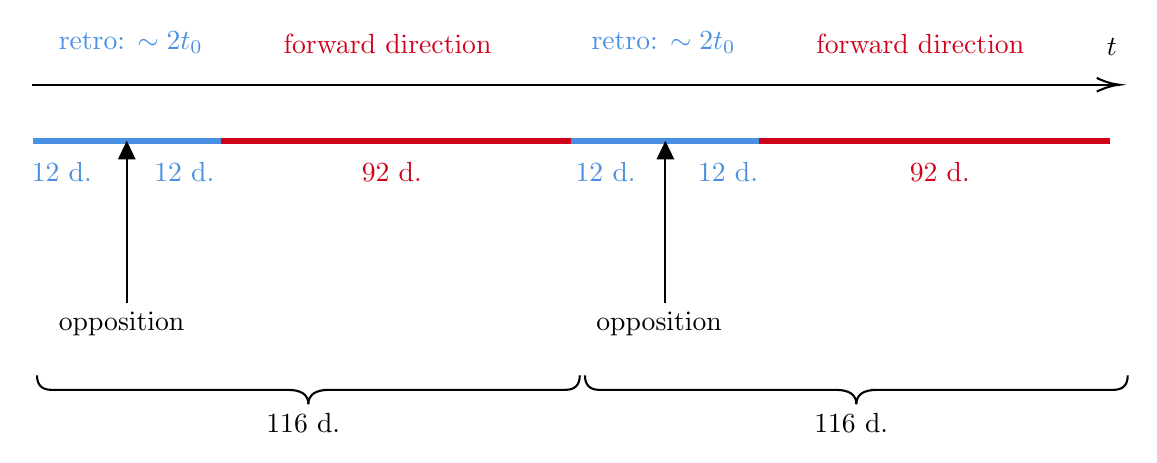
\begin{tikzpicture}[x=0.75pt,y=0.75pt,yscale=-1,xscale=1]
		%uncomment if require: \path (0,1196); %set diagram left start at 0, and has height of 1196
		
		%Straight Lines [id:da6312460542875413] 
		\draw    (58.5,80) -- (580.5,80) ;
		\draw [shift={(582.5,80)}, rotate = 180] [color={rgb, 255:red, 0; green, 0; blue, 0 }  ][line width=0.75]    (10.93,-3.29) .. controls (6.95,-1.4) and (3.31,-0.3) .. (0,0) .. controls (3.31,0.3) and (6.95,1.4) .. (10.93,3.29)   ;
		%Straight Lines [id:da9902157928743409] 
		\draw [color={rgb, 255:red, 74; green, 144; blue, 226 }  ,draw opacity=1 ][line width=2.25]    (59,107) -- (149.5,107) ;
		%Straight Lines [id:da5650800761440682] 
		\draw [color={rgb, 255:red, 208; green, 2; blue, 27 }  ,draw opacity=1 ][line width=2.25]    (149.5,107) -- (318.5,107) ;
		%Straight Lines [id:da4642989170806724] 
		\draw [color={rgb, 255:red, 74; green, 144; blue, 226 }  ,draw opacity=1 ][line width=2.25]    (318.5,107) -- (409,107) ;
		%Straight Lines [id:da7888301728846085] 
		\draw [color={rgb, 255:red, 208; green, 2; blue, 27 }  ,draw opacity=1 ][line width=2.25]    (409,107) -- (578,107) ;
		%Straight Lines [id:da11174866584972287] 
		\draw    (104.25,185) -- (104.25,110) ;
		\draw [shift={(104.25,107)}, rotate = 90] [fill={rgb, 255:red, 0; green, 0; blue, 0 }  ][line width=0.08]  [draw opacity=0] (8.93,-4.29) -- (0,0) -- (8.93,4.29) -- cycle    ;
		%Straight Lines [id:da912252982786103] 
		\draw    (363.75,185) -- (363.75,110) ;
		\draw [shift={(363.75,107)}, rotate = 90] [fill={rgb, 255:red, 0; green, 0; blue, 0 }  ][line width=0.08]  [draw opacity=0] (8.93,-4.29) -- (0,0) -- (8.93,4.29) -- cycle    ;
		%Shape: Brace [id:dp6072858090380053] 
		\draw   (61,220) .. controls (61,224.67) and (63.33,227) .. (68,227) -- (181.75,227) .. controls (188.42,227) and (191.75,229.33) .. (191.75,234) .. controls (191.75,229.33) and (195.08,227) .. (201.75,227)(198.75,227) -- (315.5,227) .. controls (320.17,227) and (322.5,224.67) .. (322.5,220) ;
		%Shape: Brace [id:dp29879882360628707] 
		\draw   (325,220) .. controls (325,224.67) and (327.33,227) .. (332,227) -- (445.75,227) .. controls (452.42,227) and (455.75,229.33) .. (455.75,234) .. controls (455.75,229.33) and (459.08,227) .. (465.75,227)(462.75,227) -- (579.5,227) .. controls (584.17,227) and (586.5,224.67) .. (586.5,220) ;
		
		% Text Node
		\draw (575,56.4) node [anchor=north west][inner sep=0.75pt]    {$t$};
		% Text Node
		\draw (70,53) node [anchor=north west][inner sep=0.75pt]  [color={rgb, 255:red, 74; green, 144; blue, 226 }  ,opacity=1 ] [align=left] {retro: $\displaystyle \sim 2t_{0}$};
		% Text Node
		\draw (178.33,54) node [anchor=north west][inner sep=0.75pt]  [color={rgb, 255:red, 208; green, 2; blue, 27 }  ,opacity=1 ] [align=left] {forward direction};
		% Text Node
		\draw (326.66,53) node [anchor=north west][inner sep=0.75pt]  [color={rgb, 255:red, 74; green, 144; blue, 226 }  ,opacity=1 ] [align=left] {retro: $\displaystyle \sim 2t_{0}$};
		% Text Node
		\draw (435,54) node [anchor=north west][inner sep=0.75pt]  [color={rgb, 255:red, 208; green, 2; blue, 27 }  ,opacity=1 ] [align=left] {forward direction};
		% Text Node
		\draw (57,116) node [anchor=north west][inner sep=0.75pt]  [color={rgb, 255:red, 74; green, 144; blue, 226 }  ,opacity=1 ] [align=left] {$\displaystyle 12$ d.};
		% Text Node
		\draw (116,116) node [anchor=north west][inner sep=0.75pt]  [color={rgb, 255:red, 74; green, 144; blue, 226 }  ,opacity=1 ] [align=left] {$\displaystyle 12$ d.};
		% Text Node
		\draw (216,116) node [anchor=north west][inner sep=0.75pt]  [color={rgb, 255:red, 208; green, 2; blue, 27 }  ,opacity=1 ] [align=left] {$\displaystyle 92$ d.};
		% Text Node
		\draw (319,116) node [anchor=north west][inner sep=0.75pt]  [color={rgb, 255:red, 74; green, 144; blue, 226 }  ,opacity=1 ] [align=left] {$\displaystyle 12$ d.};
		% Text Node
		\draw (378,116) node [anchor=north west][inner sep=0.75pt]  [color={rgb, 255:red, 74; green, 144; blue, 226 }  ,opacity=1 ] [align=left] {$\displaystyle 12$ d.};
		% Text Node
		\draw (480,116) node [anchor=north west][inner sep=0.75pt]  [color={rgb, 255:red, 208; green, 2; blue, 27 }  ,opacity=1 ] [align=left] {$\displaystyle 92$ d.};
		% Text Node
		\draw (70,188) node [anchor=north west][inner sep=0.75pt]   [align=left] {opposition};
		% Text Node
		\draw (329,188) node [anchor=north west][inner sep=0.75pt]   [align=left] {opposition};
		% Text Node
		\draw (170,237) node [anchor=north west][inner sep=0.75pt]   [align=left] {$\displaystyle 116$ d.};
		% Text Node
		\draw (434,237) node [anchor=north west][inner sep=0.75pt]   [align=left] {$\displaystyle 116$ d.};
		\end{tikzpicture}
		\vspace*{3mm}
		\caption[]{Retrogradiation cycle diagram principle}	
	\end{figure}
	\begin{tcolorbox}[title=Remark,arc=10pt,breakable,drop lifted shadow,
  skin=enhanced,
  skin first is subskin of={enhancedfirst}{arc=10pt,no shadow},
  skin middle is subskin of={enhancedmiddle}{arc=10pt,no shadow},
  skin last is subskin of={enhancedlast}{drop lifted shadow}]
	At specific points on Mercury's surface, an observer would be able to see the Sun rise part way, then reverse and set before rising again, all within the same Mercurian day. This apparent retrograde motion of the Sun occurs because, from approximately four Earth days before perihelion until approximately four Earth days after it, Mercury's angular orbital speed exceeds its angular rotational velocity. Mercury's elliptical orbit is farther from circular than that of any other planet in the Solar System, resulting in a substantially higher orbital speed near perihelion.
	\end{tcolorbox}
	\begin{figure}[H]
		\centering
		\includegraphics[scale=0.45]{img/cosmology/retrograde_motion_mars_saturn.jpg}
		\caption[Real sequence of exposures showing Mars and Saturn retrograde motion]{Real sequence of exposures showing Mars and Saturn retrograde motion (author: Tunç Tezel)}
	\end{figure}
	
	\pagebreak
	\subsection{Lagrange Points}\label{Lagrange points}
	A "\NewTerm{Lagrange point}\index{Lagrange point}" (denoted by L), or "\NewTerm{libration point}\index{libration point}" is a position in space where the gravitational fields of two bodies in orbit around each other, and of substantial masses, combine to provide an equilibrium point to a third body of negligible mass, such that the relative positions of the three bodies are fixed.

	We will in the developments that follow take time to prove (as best as we can...) that such points are at the number of $5$ denoted L1 to L5 respectively.

	It may be helpful to make a presentation of these points and their properties before going through the mathematical part. This may help in understanding the subject.

	We will immediately consider the following diagram:
	\begin{figure}[H]
		\centering
		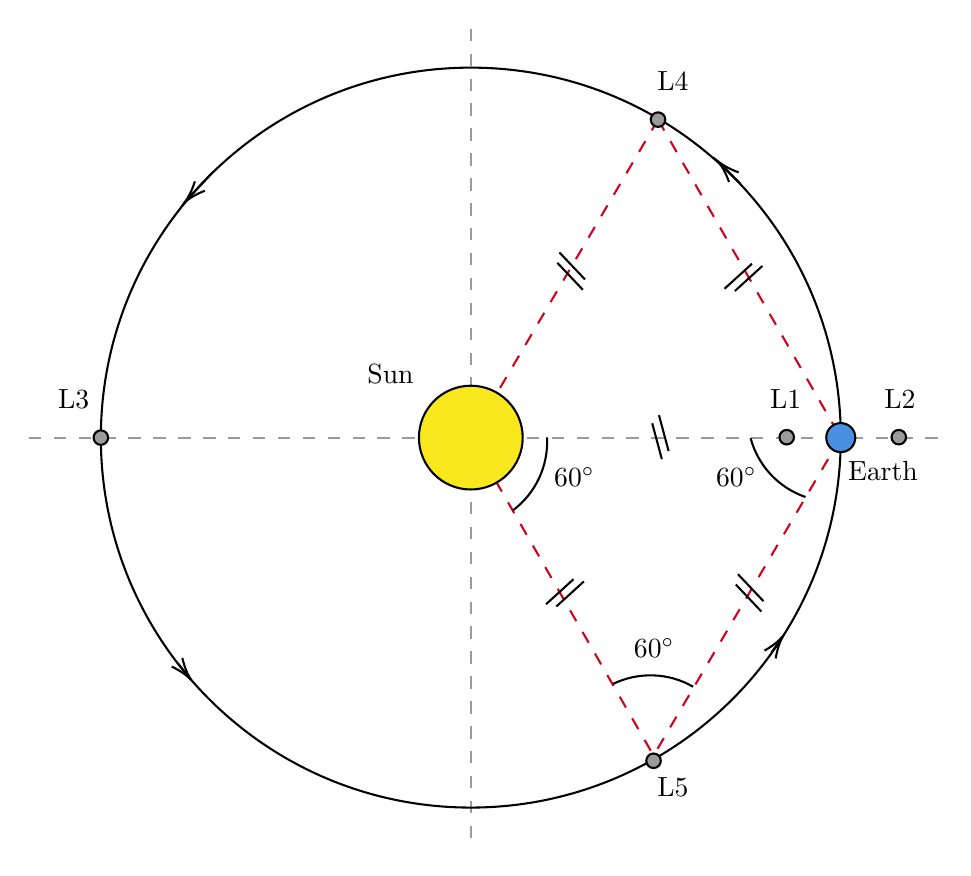
\begin{tikzpicture}[x=0.75pt,y=0.75pt,yscale=-1,xscale=1]
		%uncomment if require: \path (0,592); %set diagram left start at 0, and has height of 592
		
		%Straight Lines [id:da5789822586452666] 
		\draw [color={rgb, 255:red, 208; green, 2; blue, 27 }  ,draw opacity=1 ] [dash pattern={on 4.5pt off 4.5pt}]  (401.5,42) -- (489.55,195.2) ;
		%Straight Lines [id:da6551645325360838] 
		\draw [color={rgb, 255:red, 155; green, 155; blue, 155 }  ,draw opacity=1 ] [dash pattern={on 4.5pt off 4.5pt}]  (311.3,-1.8) -- (311.3,392.2) ;
		%Straight Lines [id:da3011009743883808] 
		\draw [color={rgb, 255:red, 155; green, 155; blue, 155 }  ,draw opacity=1 ] [dash pattern={on 4.5pt off 4.5pt}]  (98.3,195.2) -- (538.3,195.2) ;
		%Shape: Circle [id:dp5850620640292046] 
		\draw   (133.05,195.2) .. controls (133.05,96.76) and (212.86,16.95) .. (311.3,16.95) .. controls (409.74,16.95) and (489.55,96.76) .. (489.55,195.2) .. controls (489.55,293.64) and (409.74,373.45) .. (311.3,373.45) .. controls (212.86,373.45) and (133.05,293.64) .. (133.05,195.2) -- cycle ;
		%Shape: Circle [id:dp7453195150645615] 
		\draw  [fill={rgb, 255:red, 155; green, 155; blue, 155 }  ,fill opacity=1 ] (460,195) .. controls (460,193.07) and (461.57,191.5) .. (463.5,191.5) .. controls (465.43,191.5) and (467,193.07) .. (467,195) .. controls (467,196.93) and (465.43,198.5) .. (463.5,198.5) .. controls (461.57,198.5) and (460,196.93) .. (460,195) -- cycle ;
		%Shape: Circle [id:dp7754075387586714] 
		\draw  [fill={rgb, 255:red, 155; green, 155; blue, 155 }  ,fill opacity=1 ] (514,195) .. controls (514,193.07) and (515.57,191.5) .. (517.5,191.5) .. controls (519.43,191.5) and (521,193.07) .. (521,195) .. controls (521,196.93) and (519.43,198.5) .. (517.5,198.5) .. controls (515.57,198.5) and (514,196.93) .. (514,195) -- cycle ;
		%Straight Lines [id:da4661880693953113] 
		\draw [color={rgb, 255:red, 208; green, 2; blue, 27 }  ,draw opacity=1 ] [dash pattern={on 4.5pt off 4.5pt}]  (401.5,42) -- (311.3,195.2) ;
		%Straight Lines [id:da399763777232512] 
		\draw [color={rgb, 255:red, 208; green, 2; blue, 27 }  ,draw opacity=1 ] [dash pattern={on 4.5pt off 4.5pt}]  (489.55,195.2) -- (399.35,348.4) ;
		%Straight Lines [id:da7155436034888958] 
		\draw [color={rgb, 255:red, 208; green, 2; blue, 27 }  ,draw opacity=1 ] [dash pattern={on 4.5pt off 4.5pt}]  (311.3,195.2) -- (399.35,348.4) ;
		%Shape: Circle [id:dp7541935440399226] 
		\draw  [fill={rgb, 255:red, 155; green, 155; blue, 155 }  ,fill opacity=1 ] (129.55,195.2) .. controls (129.55,193.27) and (131.12,191.7) .. (133.05,191.7) .. controls (134.98,191.7) and (136.55,193.27) .. (136.55,195.2) .. controls (136.55,197.13) and (134.98,198.7) .. (133.05,198.7) .. controls (131.12,198.7) and (129.55,197.13) .. (129.55,195.2) -- cycle ;
		%Straight Lines [id:da908364624702581] 
		\draw    (353,111) -- (365.3,124) ;
		%Straight Lines [id:da9617247586748436] 
		\draw    (354,106) -- (366.3,119) ;
		%Straight Lines [id:da14868739554629906] 
		\draw    (398.7,188.32) -- (403.34,205.6) ;
		%Straight Lines [id:da08490803557884452] 
		\draw    (401.96,184.4) -- (406.6,201.68) ;
		%Straight Lines [id:da4519293392761716] 
		\draw    (446.78,111.43) -- (433.54,123.48) ;
		%Straight Lines [id:da9085348503744943] 
		\draw    (451.76,112.52) -- (438.52,124.57) ;
		%Straight Lines [id:da532941783551161] 
		\draw    (360.78,263.43) -- (347.54,275.48) ;
		%Straight Lines [id:da7031489198143868] 
		\draw    (365.76,264.52) -- (352.52,276.57) ;
		%Straight Lines [id:da6029811784037182] 
		\draw    (439,266) -- (451.3,279) ;
		%Straight Lines [id:da8771426979657155] 
		\draw    (440,261) -- (452.3,274) ;
		%Straight Lines [id:da6616399059183082] 
		\draw    (187.3,67) -- (174.66,80.54) ;
		\draw [shift={(173.3,82)}, rotate = 313.03] [color={rgb, 255:red, 0; green, 0; blue, 0 }  ][line width=0.75]    (10.93,-3.29) .. controls (6.95,-1.4) and (3.31,-0.3) .. (0,0) .. controls (3.31,0.3) and (6.95,1.4) .. (10.93,3.29)   ;
		%Straight Lines [id:da6957258354415721] 
		\draw    (441.3,73) -- (431.71,63.41) ;
		\draw [shift={(430.3,62)}, rotate = 45] [color={rgb, 255:red, 0; green, 0; blue, 0 }  ][line width=0.75]    (10.93,-3.29) .. controls (6.95,-1.4) and (3.31,-0.3) .. (0,0) .. controls (3.31,0.3) and (6.95,1.4) .. (10.93,3.29)   ;
		%Straight Lines [id:da8493091350434372] 
		\draw    (456.16,298.76) -- (460.61,292.4) ;
		\draw [shift={(461.76,290.76)}, rotate = 124.99] [color={rgb, 255:red, 0; green, 0; blue, 0 }  ][line width=0.75]    (10.93,-3.29) .. controls (6.95,-1.4) and (3.31,-0.3) .. (0,0) .. controls (3.31,0.3) and (6.95,1.4) .. (10.93,3.29)   ;
		%Straight Lines [id:da9303773288200587] 
		\draw    (170.16,303.96) -- (175.31,310.4) ;
		\draw [shift={(176.56,311.96)}, rotate = 231.34] [color={rgb, 255:red, 0; green, 0; blue, 0 }  ][line width=0.75]    (10.93,-3.29) .. controls (6.95,-1.4) and (3.31,-0.3) .. (0,0) .. controls (3.31,0.3) and (6.95,1.4) .. (10.93,3.29)   ;
		%Shape: Arc [id:dp6658970864886122] 
		\draw  [draw opacity=0] (348.02,195.07) .. controls (348.75,208.67) and (342.65,221.92) .. (331.68,230.18) -- (306.9,197.29) -- cycle ; \draw   (348.02,195.07) .. controls (348.75,208.67) and (342.65,221.92) .. (331.68,230.18) ;  
		%Shape: Circle [id:dp9737767914135551] 
		\draw  [fill={rgb, 255:red, 248; green, 231; blue, 28 }  ,fill opacity=1 ] (286.3,195.2) .. controls (286.3,181.39) and (297.49,170.2) .. (311.3,170.2) .. controls (325.11,170.2) and (336.3,181.39) .. (336.3,195.2) .. controls (336.3,209.01) and (325.11,220.2) .. (311.3,220.2) .. controls (297.49,220.2) and (286.3,209.01) .. (286.3,195.2) -- cycle ;
		%Shape: Arc [id:dp8518164683281351] 
		\draw  [draw opacity=0] (472.55,223.82) .. controls (459.67,219.41) and (449.67,208.79) .. (446.12,195.52) -- (485.9,184.87) -- cycle ; \draw   (472.55,223.82) .. controls (459.67,219.41) and (449.67,208.79) .. (446.12,195.52) ;  
		%Shape: Circle [id:dp4143112736998109] 
		\draw  [fill={rgb, 255:red, 155; green, 155; blue, 155 }  ,fill opacity=1 ] (395.85,350.9) .. controls (395.85,348.97) and (397.42,347.4) .. (399.35,347.4) .. controls (401.28,347.4) and (402.85,348.97) .. (402.85,350.9) .. controls (402.85,352.83) and (401.28,354.4) .. (399.35,354.4) .. controls (397.42,354.4) and (395.85,352.83) .. (395.85,350.9) -- cycle ;
		%Shape: Circle [id:dp21964114835567328] 
		\draw  [fill={rgb, 255:red, 155; green, 155; blue, 155 }  ,fill opacity=1 ] (398,42) .. controls (398,40.07) and (399.57,38.5) .. (401.5,38.5) .. controls (403.43,38.5) and (405,40.07) .. (405,42) .. controls (405,43.93) and (403.43,45.5) .. (401.5,45.5) .. controls (399.57,45.5) and (398,43.93) .. (398,42) -- cycle ;
		%Shape: Circle [id:dp038745013552865304] 
		\draw  [fill={rgb, 255:red, 74; green, 144; blue, 226 }  ,fill opacity=1 ] (482.55,195.2) .. controls (482.55,191.33) and (485.68,188.2) .. (489.55,188.2) .. controls (493.42,188.2) and (496.55,191.33) .. (496.55,195.2) .. controls (496.55,199.07) and (493.42,202.2) .. (489.55,202.2) .. controls (485.68,202.2) and (482.55,199.07) .. (482.55,195.2) -- cycle ;
		%Shape: Arc [id:dp6281605463493092] 
		\draw  [draw opacity=0] (379.74,313.92) .. controls (391.97,307.93) and (406.55,308.37) .. (418.44,315.24) -- (397.85,350.9) -- cycle ; \draw   (379.74,313.92) .. controls (391.97,307.93) and (406.55,308.37) .. (418.44,315.24) ;  
		
		% Text Node
		\draw (260,158.4) node [anchor=north west][inner sep=0.75pt]   [align=left] {Sun};
		% Text Node
		\draw (491.55,205.2) node [anchor=north west][inner sep=0.75pt]   [align=left] {Earth};
		% Text Node
		\draw (454,170.5) node [anchor=north west][inner sep=0.75pt]   [align=left] {L1};
		% Text Node
		\draw (509,170.5) node [anchor=north west][inner sep=0.75pt]   [align=left] {L2};
		% Text Node
		\draw (111,170.5) node [anchor=north west][inner sep=0.75pt]   [align=left] {L3};
		% Text Node
		\draw (399.67,17.5) node [anchor=north west][inner sep=0.75pt]   [align=left] {L4};
		% Text Node
		\draw (399.67,357.4) node [anchor=north west][inner sep=0.75pt]   [align=left] {L5};
		% Text Node
		\draw (350,207.9) node [anchor=north west][inner sep=0.75pt]    {$60^{\circ }$};
		% Text Node
		\draw (428,207.9) node [anchor=north west][inner sep=0.75pt]    {$60^{\circ }$};
		% Text Node
		\draw (388.4,290.7) node [anchor=north west][inner sep=0.75pt]    {$60^{\circ }$};
		\end{tikzpicture}
		\vspace*{3mm}
		\caption{Representation of the five Lagrangian point in the Sun-Earth system}	
	\end{figure}
	There are five Lagrange points:
	\begin{enumerate}
		\item[L1:] On the line defined by the both masses between them (this is the most easy point to interpret intuitively: it is for example the point where the gravitational attraction of the Sun is compensated by that of the Earth).

		\begin{tcolorbox}[colframe=black,colback=white,sharp corners,breakable]
		\textbf{{\Large \ding{45}}Example:}\\\\
		We consider an object orbiting around the Sun, closer to the latter than the Earth but on the same line. This object undergoes a solar gravity greater than that of Earth, and therefore spins faster around the Sun than does the Earth. But Earth's gravity partially counteracts that of the Sun, which slows it down. The more we approaches this object of the Earth the more this counteract effect is important. At some point, the point L1, the angular speed of the object becomes exactly equal to that of the Earth.
		\end{tcolorbox}
		

		\item[L2:] On the line defined by the both masses, beyond the smaller (a bit less intuitive as is the point where the cumulative effect of the Sun and Earth will compensate the centrifugal force).

		\begin{tcolorbox}[colframe=black,colback=white,sharp corners,breakable]
		\textbf{{\Large \ding{45}}Example:}\\\\
		The principle is similar to the previous case, but on the other side of the Earth. The object should rotate more slowly than Earth because the solar gravity is lower, but the extra gravitational field due to the Earth tends to accelerate it. At some point, the point L2, the object rotates at exactly the same angular velocity as the Earth around the Sun.
		\end{tcolorbox}
		
		\item[L3:] On the line defined by the two masses, beyond the larger (intuitive based on physical considerations: it is clear that an object diametrically opposite to the Earth relatively to the Sun would have the same orbital period as the Earth and therefore would be fixed relative to the Earth-Sun system).

		\begin{tcolorbox}[colframe=black,colback=white,sharp corners,breakable]
		\textbf{{\Large \ding{45}}Example:}\\\\
		Identically to the L2 point, there exists a point a little further away than the Earth relatively the Sun, where a negligible mass object would be in equilibrium.
		\end{tcolorbox}
		

		\item[L4 \& L5:] On the apexes of two equilateral triangles whose base is formed by the two masses.
		
		\begin{tcolorbox}[colframe=black,colback=white,sharp corners,breakable]
		\textbf{{\Large \ding{45}}Example:}\\\\
		This is a subtle balance between the centripetal force exerted by the two main masses and the centrifugal force of the masses considered at the points of interest. L4 is ahead of the smaller mass in its orbit around the large one, and L5 is late. These two points are sometimes named "\NewTerm{triangular Lagrange points}\index{triangular Lagrange points}" or "\NewTerm{Trojans point}\index{Trojans point}".\\

	Remarkably, the last two points do not depend on the relative masses of the two bodies as we will prove it.
		\end{tcolorbox}

	\end{enumerate}
	For the first three Lagrangian points, stability appears only in the plane perpendicular to the line occupied by the two masses. For example, for the L1 point, if we move an object perpendicular to the line between the two masses, the two gravitational forces will play to bring it back to the starting position. The equilibrium is stable. However, if we move it near to one the two masses, then the field of that latter will prevail over the other and the object will tend to get closer. The equilibrium is unstable. For L4 and L5 points, stability is obtained due to Coriolis forces acting on the objects moving away from the point.
	
	Given the stability issues given above, we have no natural object around point L1, L2 and L3 at least in the solar system. However, they still represent an interest in scientific achievements because they allow savings of fuel for orbit control and attitude. This is not valid for point L3, due to its distance from Earth which only application what that utopic one made by Sci-Fi and comic books authors that place an Anti-Earth twin-planet but which mass was too high in relation to the theory stated above. However, space missions use L1 and L2: the case of the probe SOHO since 11995 according to holocene calendar (Solar and Heliospheric Observatory) a Sun observation station located at L1 (1.5 million kilometres from Earth) or MAP (Wilkinson Microwave Anisotropy Probe) satellite or Planck satellite (to study the cosmic microwave background at $2.7$ [K]) close to the point L2 as will be the James Webb telescope in 12021 (the radiation of Earth there are relatively low and those of the Sun attenuated by the Earth which do a screening effect).
	
	\begin{figure}[H]
		\centering
		\includegraphics[width=0.8\textwidth]{img/cosmology/james_webb_L2.jpg}
	\end{figure}
	
	The points L4 and L5 being stable, we find many natural celestial objects. In the Sun-Jupiter system, hundreds of asteroids, known as "Trojan asteroids", clump there together (around $1,800$ identified in April 12005 according to holocene calendar). We count also  some in the Neptune-Sun systems and Mars-Sun system. Curiously, it seems that the Saturn-Sun system is not be able to accumulate such celestial objects because of the Jovian disruption. We also find objects to these points in the Saturn planetary system of Saturn: Saturn-Tethys with Telesto and Calypso with the L4 and L5 points and Saturn-Dione with Helen to the point L4 and Pollux at the L5 point. In the Sun-Earth system, there is no known large object to the Trojans points, but it was discovered a slight over-abundance of dust in 11950 (holocene calendar). Slight dust clouds are also present for the system Earth-Moon; this make scientific abandon the idea to place there a space telescope as it was envisaged once.
	
	Strictly speaking, these 5 points exist only for two bodies in circular rotation one around the other. Once the orbit of the two bodies is elliptical, these points are no longer equilibrium points. In practice, if the orbit is slightly elliptical, as is the case for real planets, we can find stable orbits oscillating not departing too much of the regions corresponding to the Lagrangian points and this is well named a "\NewTerm{halo orbit}\index{halo orbit}". Therefore the halo orbit is a periodic, three-dimensional orbit near the L1, L2 or L3 Lagrange points in the three-body problem of orbital mechanics. Although the Lagrange point is just a point in empty space, its peculiar characteristic is that it can be orbited by a special kind of orbit named "\NewTerm{Lissajous orbit}\index{Lissajous orbit}\label{Lissajous orbit}". The first mission to use a halo orbit was ISEE-3, launched in 11978 (holocene calendar). It travelled as we already mention to the Sun–Earth L1 point and remained there for several years. The next mission to use a halo orbit was in fact Solar and Heliospheric Observatory (SOHO), a joint ESA and NASA mission to study the Sun, which arrived at Sun–Earth L1 in 11996 (holocene calendar). It used an orbit similar to ISEE-3.
	
	So we will consider in space an isolated system of two bodies $A$ and $B$, of mass $M_A$ and $M_B$ in gravitational interaction. These two bodies are assumed to be in circular orbit (for simplicity!) one around the other, in the manner of a two-star system (binary system) or a planet-satellite like system (Saturn-Titan example). We seek to determine if there are relative equilibrium point to the system of the two rotating body for  a third body also in circular motion in the same plane (of sufficiently low mass to avoid disturbing the motion of the system of the two main bodies).
	\begin{figure}[H]
		\centering
		\begin{tikzpicture}[x=0.75pt,y=0.75pt,yscale=-1,xscale=1]
		%uncomment if require: \path (0,1215); %set diagram left start at 0, and has height of 1215
		
		%Shape: Axis 2D [id:dp1834894618059113] 
		\draw  (107.13,361.69) -- (571.17,176.27)(161.54,64.34) -- (267.68,329.99) (562.81,174.22) -- (571.17,176.27) -- (566.52,183.51) (159.49,72.69) -- (161.54,64.34) -- (168.78,68.98)  ;
		%Flowchart: Summing Junction [id:dp895245393415119] 
		\draw   (247.5,302) .. controls (247.5,297.03) and (251.53,293) .. (256.5,293) .. controls (261.47,293) and (265.5,297.03) .. (265.5,302) .. controls (265.5,306.97) and (261.47,311) .. (256.5,311) .. controls (251.53,311) and (247.5,306.97) .. (247.5,302) -- cycle ; \draw   (250.14,295.64) -- (262.86,308.36) ; \draw   (262.86,295.64) -- (250.14,308.36) ;
		%Straight Lines [id:da9523460776933002] 
		\draw [color={rgb, 255:red, 208; green, 2; blue, 27 }  ,draw opacity=1 ][line width=1.5]    (256.5,302) -- (231.97,239.72) ;
		\draw [shift={(230.5,236)}, rotate = 68.5] [fill={rgb, 255:red, 208; green, 2; blue, 27 }  ,fill opacity=1 ][line width=0.08]  [draw opacity=0] (11.61,-5.58) -- (0,0) -- (11.61,5.58) -- cycle    ;
		%Straight Lines [id:da4672352117535321] 
		\draw [color={rgb, 255:red, 208; green, 2; blue, 27 }  ,draw opacity=1 ][line width=1.5]    (256.5,302) -- (320.78,276.48) ;
		\draw [shift={(324.5,275)}, rotate = 158.34] [fill={rgb, 255:red, 208; green, 2; blue, 27 }  ,fill opacity=1 ][line width=0.08]  [draw opacity=0] (11.61,-5.58) -- (0,0) -- (11.61,5.58) -- cycle    ;
		%Straight Lines [id:da35782354736011945] 
		\draw [color={rgb, 255:red, 0; green, 0; blue, 0 }  ,draw opacity=1 ][line width=1.5]    (256.5,302) -- (329.05,114.73) ;
		\draw [shift={(330.5,111)}, rotate = 111.18] [fill={rgb, 255:red, 0; green, 0; blue, 0 }  ,fill opacity=1 ][line width=0.08]  [draw opacity=0] (11.61,-5.58) -- (0,0) -- (11.61,5.58) -- cycle    ;
		%Shape: Circle [id:dp595066926449888] 
		\draw  [fill={rgb, 255:red, 0; green, 0; blue, 0 }  ,fill opacity=1 ] (324,111) .. controls (324,107.41) and (326.91,104.5) .. (330.5,104.5) .. controls (334.09,104.5) and (337,107.41) .. (337,111) .. controls (337,114.59) and (334.09,117.5) .. (330.5,117.5) .. controls (326.91,117.5) and (324,114.59) .. (324,111) -- cycle ;
		%Shape: Circle [id:dp7765048303145505] 
		\draw  [fill={rgb, 255:red, 0; green, 0; blue, 0 }  ,fill opacity=1 ] (476.5,210.75) .. controls (476.5,206.19) and (480.19,202.5) .. (484.75,202.5) .. controls (489.31,202.5) and (493,206.19) .. (493,210.75) .. controls (493,215.31) and (489.31,219) .. (484.75,219) .. controls (480.19,219) and (476.5,215.31) .. (476.5,210.75) -- cycle ;
		%Shape: Circle [id:dp5381019368944424] 
		\draw  [fill={rgb, 255:red, 0; green, 0; blue, 0 }  ,fill opacity=1 ] (140.5,345.75) .. controls (140.5,341.19) and (144.19,337.5) .. (148.75,337.5) .. controls (153.31,337.5) and (157,341.19) .. (157,345.75) .. controls (157,350.31) and (153.31,354) .. (148.75,354) .. controls (144.19,354) and (140.5,350.31) .. (140.5,345.75) -- cycle ;
		%Shape: Arc [id:dp6688141164231127] 
		\draw  [draw opacity=0][dash pattern={on 4.5pt off 4.5pt}] (271.78,42.46) .. controls (342.09,46.54) and (404.9,78.55) .. (449.28,127.57) -- (256.5,302) -- cycle ; \draw [dash pattern={on 4.5pt off 4.5pt}] [dash pattern={on 4.5pt off 4.5pt}]  (274.94,42.67) .. controls (343.97,47.5) and (405.56,79.29) .. (449.28,127.57) ;  \draw [shift={(271.78,42.46)}, rotate = 4.7] [fill={rgb, 255:red, 0; green, 0; blue, 0 }  ][dash pattern={on 3.49pt off 4.5pt}][line width=0.08]  [draw opacity=0] (8.93,-4.29) -- (0,0) -- (8.93,4.29) -- cycle    ;
		
		% Text Node
		\draw (140,62.4) node [anchor=north west][inner sep=0.75pt]    {$y$};
		% Text Node
		\draw (575,173.4) node [anchor=north west][inner sep=0.75pt]    {$x$};
		% Text Node
		\draw (230,285) node [anchor=north west][inner sep=0.75pt]   [align=left] {O};
		% Text Node
		\draw (213,235.4) node [anchor=north west][inner sep=0.75pt]  [color={rgb, 255:red, 208; green, 2; blue, 27 }  ,opacity=1 ]  {$\vec{j}$};
		% Text Node
		\draw (321,280.4) node [anchor=north west][inner sep=0.75pt]  [color={rgb, 255:red, 208; green, 2; blue, 27 }  ,opacity=1 ]  {$\vec{i}$};
		% Text Node
		\draw (246,314.4) node [anchor=north west][inner sep=0.75pt]  [color={rgb, 255:red, 208; green, 2; blue, 27 }  ,opacity=1 ]  {$\vec{k}$};
		% Text Node
		\draw (341,102.4) node [anchor=north west][inner sep=0.75pt]    {$S$};
		% Text Node
		\draw (306,179.4) node [anchor=north west][inner sep=0.75pt]    {$\vec{r}$};
		% Text Node
		\draw (159,349.15) node [anchor=north west][inner sep=0.75pt]    {$A$};
		% Text Node
		\draw (495,214.15) node [anchor=north west][inner sep=0.75pt]    {$B$};
		% Text Node
		\draw (271,55.4) node [anchor=north west][inner sep=0.75pt]    {$R'$};
		\end{tikzpicture}
	\end{figure}
	Let O be the centroid (\SeeChapter{see section Classical Mechanics page \pageref{center of mass}}) of these two stars (or celestial objects in general). Let us consider a Galilean reference frame (in rectilinear and uniform motion therefore !) or origin O. Compared to this reference frame, we assume that the axis $AB$ rotates at a constant angular velocity $\omega$ of fixed axis $\vec{k}$ (perpendicular to the page in the figure and directed towards the reader) and that the distances $r_A=\overline{A\text{O}}$ and $r_B=\overline{B\text{O}}$ also remain constant.
 
 We know from our study of Classical Mechanics that a circular motion the centrifugal force is given by (see page \pageref{centrifugal force}):
	
	So we have (equilibrium between centrifugal and centripetal forces) to guarantee the equilibrium:
	
	By simplifying and summing these two relations:
	By simplifying and summing these two relations:
	
	with in what will follow $AB=r_A+r_B=R$.
	
	Let us consider a rotating reference frame $R'$ linked to our stars as shown in figure above: $\vec{i}$ will be a collinear unit vector to $AB$, $\vec{j}$ a unit vector perpendicular to $\vec{i}$ and in the rotating plane of the planets and finally $\vec{k}=\vec{i}\times\vec{j}$ collinear to $\vec{\omega}$.

	We consider in this rotating frame (with stars) a third star $S$ of mass $m$ negligible relatively to $M_A$ and $M_B$, subject to the gravitational attraction of $A$ and $B$.

	Now let us denote by $\vec{a}_{R'}$ the acceleration of $S$ with respect to $R'$, $\vec{v}_{R'}$ its speed and $\vec{e}_r$ the collinear  unit vector to $\overrightarrow{\text{O}S'}$ where $S'$ is the projection of $S$ in the plane O$xy$, and $r=\overline{\text{O}S'}$ (in the figure above, we assumed $S$ in the plane O$xy$, so $S$ and $S'$ are indistinguishable).
	
	$S$ is thus subjected to two forces, one $\vec{F}_A$ directed along $A$ and the other $\vec{F}_B$ directed along $B$, forces of respective intensities :
	
	In a Galilean reference frame, these two forces apply to $S$ an acceleration given by the law of composition of accelerations in a circular reference frame (\SeeChapter{see section Classical Mechanics page \pageref{relative movements and inertial forces}}):
	
	But, in our configuration the pulsation (radial velocity) is assumed constant and the drive acceleration is zero since we assumed $R'$ as the main repository. Therefore it comes:
	
	We also have:
	
	where according to the figure all components are positive. The calculation of the cross product then gives (\SeeChapter{see section Vector Calculus page \pageref{cross product}}):
	
	So finally:
	
	Let us rather write this relation into the form:
	
	We then obtain, by projecting on the three axes $x$, $y$ and $z$, the derivatives taken with respect to time $t$ the following system:
	
	with:
	
	so that the coordinates $(x,y,z)$ of the point $S$ are those of an equilibrium point, then it is trivial that in the rotating frame with the stars $A$ and $B$ that:
	
	We then get the following system:
	
	It is also immediately that the third equation has for only solution $z=0$ and thus ultimately the system reduces to:
	
	The third equation simply means that the equilibrium positions are in the plane O$xy$ (we could suspect it a bit ...). The other two, we will see it later, lead us to consider five solutions that are our five Lagrangian points L1, ..., L5.

	If we draw plot with an appropriate software the acceleration (respectively force) with the isoclines highlighted (curves on which the acceleration is equal) we get:
	\begin{figure}[H]
		\centering
		\includegraphics[scale=1]{img/cosmology/lagrange_points_two_bodies_isoclines_plot_3d.jpg}	
		\caption{Isoclines of the two-body system}
	\end{figure}
	where we see that a short distance of the bodies the gravitational potential energy dominates, but that a large distances the centrifugal potential predominates and the shape of the surface is similar to that of a paraboloid.

	By requesting the software to plot only the isoclines projected on a plane we get:
	\begin{figure}[H]
		\centering
		\includegraphics[scale=1]{img/cosmology/lagrange_points_two_bodies_isoclines_plot_2d.jpg}	
		\caption{Projected isoclines of the two body system on a plane}
	\end{figure}
	where we have highlighted the five Lagrange points and where the stars (or celestial objects) are represented by blue dots and the centroid of the system by a green dot. It seems that isoclines are named in the astronomy field "\NewTerm{Roche equipotentials lobes}". Otherwise seen:
	\begin{figure}[H]
		\centering
		\includegraphics[scale=1]{img/cosmology/lagrange_points_two_bodies_isoclines_plot_2d_and_3d.jpg}	
		\caption[]{Projected isoclines of the two body system on a plane}
	\end{figure}
	For those wishing to reproduce these figures with MATLAB™ here is how first proceed mathematically. From what we got previously, we have explicitly and in writing in a more academic form, the following relation:
	
	As the point $S$ is supposedly in equilibrium the last term vanishes (its speeds are zero in the rotating frame!). It then remains:
	
	We have proved for recall in the section of Classical Mechanics that:
	
	Then we have:
	
	Thus taken by unit mass of the satellite:
	
	The application of these relations in MATLAB™ 2013a then gives (sorry it's a bit long and its probably possible to do better ...):
	\begin{lstlisting}[language=MATLAB]
		%We build the grid plot that we will by anticipation densifiate where are the objects of interest
		x1=linspace(-7E8,-8E5,150);
		x2=linspace(8E5,1.2E8,150);
		x3=linspace(1.6E8,7E8,150);
		x=x1+x2+x3;
		y=linspace(-7E8,7E8,450);
		[X,Y]=meshgrid(x,y);
		%These masses and G are real but the rest is fictitious so that the plot is readable 
		f=@(x,y) -(1.3346E20)./(sqrt((x-450).^2+y.^2))-(1.0038E19)./(sqrt((x-449999550).^2+y.^2))-(6.9E-7.*(x.^2+y.^2));
		z=f(X,Y);
		%We eliminate the values that are too big on Z to have an esthetical result to see
		for i=1:450;
		   for j=1:150;
		      if (z(i,j)<-0.8E12) %to do with meshc a nice plot, limit to  -8E11
		         z(i,j)=-0.8E12;
		      end; 
		   end; 
		end; 
		contour(X,Y,z,100); mesh(X,Y,z); meshc(X,Y,z); 
		az = 100; el = 25; view(az, el);
		axis([-7E8 7E8 -0.8E9 0.8E9 -8E11 -4E11]);
		colorbar; light; camlight('right');
	\end{lstlisting}
	That gives:
	\begin{figure}[H]
		\centering
		\includegraphics[scale=1]{img/cosmology/lagrange_points_two_bodies_3d_matlab.jpg}
		\caption{Lagrange plot and isoclines in 3D with MATLAB™ 2013a}
	\end{figure}
	Or in 2D:
	\begin{lstlisting}[language=MATLAB]
		%  Author: David J. Muraki
		%  15 jan 2004
		%  coordinates
		
		L = 15;  xr =  -L:0.05:L;  xi = xr;
		
		[zr zi] = meshgrid(xr,xi);  zz = zr + i*zi;
		
		%  first integral
		GMs = 10.0;  Gme =  1.0;  R = 10;
		As  = - R*Gme/(GMs+Gme);
		ae  =   R*GMs/(GMs+Gme);
		om2 = (GMs+Gme)/(R^3);
		
		pot = om2*abs(zz).^2 + 2*GMs./abs(zz-As) + 2*Gme./abs(zz-ae);
		
		force = om2*zz ... 
		      - GMs*(zz-As)./(abs(zz-As).^3) - Gme*(zz-ae)./(abs(zz-ae).^3);
		
		%  contourplot
		figure(1);  clf;  hold on
		contour(xr,xi,pot,[3.2:0.05:4]);
		axis([-1 1 -1 1]*L);  
		axis square;  colorbar
		hold on
		plot(As,0,'k*');  plot(ae,0,'k*')
		
		ptitle = ['\bf potential energy & zero force contours'];
		title(ptitle)
		xlabel('\bf Re(x)')
		ylabel('\bf Im(x)')
		
		contour(xr,xi,real(force),[0 0],'k');
		contour(xr,xi,imag(force),[0 0],'k--');
	\end{lstlisting}
	That gives:
	\begin{figure}[H]
		\centering
		\includegraphics[scale=0.75]{img/cosmology/lagrange_points_two_bodies_2d_matlab.jpg}
		\caption{Lagrange plot and isoclines in 2D with MATLAB™ 2013a}
	\end{figure}
	Some readers will notice that it is quite difficult to intuitively build such a potential configuration just by mind! In the rotating frame with the centroid of the two solid bodies, the potential resulting from the combination of rotational and gravitational potentials present three extrema L1, L2 and L3 on the right containing the both bodies. One of these maxima is between the two bodies as expected intuitively. The other two maxima are on the line connecting the two objects, but both on either side... which is more surprising. They come from the contribution to the potential of the rotating frame which can be difficult to model intuitively.
	
	\subsubsection{Equilibrium points of the first type}
	What we mean by equilibrium positions of the first type are simply solutions located on the line $\overline{AB}$ such that $y=0$ which is equivalent to study only:
	
	with therefore:
	
	To this situation, we will consider three possible corresponding sub-cases respectively L1, L2 and L3 as we will immediately see it.
	
	\paragraph{L1 Lagrange point}\mbox{}\\\\\
	In this first sub-case, we consider:
	
	What is also equivalent to have:
	
	This allows us to write:
	
	in the following simplified form:
	
	Now to be able to say something about the possible solutions to this equation derive the left hand side. We then get:
	
	This term is strictly increasing from $-\infty$ to $+\infty$ when $x$ describes $]-r_A,r_B[$. So there is a unique solution and equilibrium point denoted L1 (first Lagrange point) between $A$ and $B$.

	If we typically consider the Sun-Earth case where $M_A>M_B$ and therefore $r_A<r_B$ then on $x=0$ we have:
	
	what is immediately negative. The equilibrium position will be obtained for a positive value of $x$ we will have to determine.

	This value can be obtained by considering a limit case: when $M_B$ tends to $0$ (corresponding to a massive celestial object $A$ turning around a mass $B$ of a much much smaller celestial object), then $A$ tends to O, $r_A$ tends to $0$ and therefore:
	
	with $R=\overline{AB}$. Therefore, in this limit case:
	
	becomes in approximation:
	
	and therefore:
	
	So the only value of $x$ satisfying this relation will be $x=R$.

	In other words, the equilibrium point L1 we are looking after here is between $A$ and $B$ moves near $B$, that is near the less massive celestial object (which corresponds well to the first figure that we used to show the location of the five Lagrange points).

	By this observation we can make the following calculations: 
	\begin{figure}[H]
		\centering
		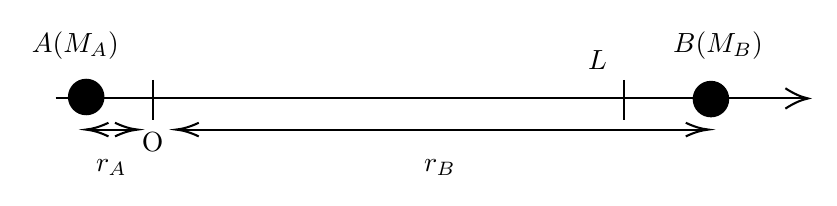
\begin{tikzpicture}[x=0.75pt,y=0.75pt,yscale=-1,xscale=1]
		%uncomment if require: \path (0,1046); %set diagram left start at 0, and has height of 1046
		
		%Straight Lines [id:da563900420095719] 
		\draw    (128,95) -- (488.5,95) ;
		\draw [shift={(490.5,95)}, rotate = 180] [color={rgb, 255:red, 0; green, 0; blue, 0 }  ][line width=0.75]    (10.93,-4.9) .. controls (6.95,-2.3) and (3.31,-0.67) .. (0,0) .. controls (3.31,0.67) and (6.95,2.3) .. (10.93,4.9)   ;
		%Straight Lines [id:da2537937486626065] 
		\draw    (175,86.1) -- (175,105.5) ;
		%Straight Lines [id:da6429853426946757] 
		\draw    (402,86.1) -- (402,105.5) ;
		%Shape: Circle [id:dp2603731885714886] 
		\draw  [fill={rgb, 255:red, 0; green, 0; blue, 0 }  ,fill opacity=1 ] (435.4,95.3) .. controls (435.4,90.72) and (439.12,87) .. (443.7,87) .. controls (448.28,87) and (452,90.72) .. (452,95.3) .. controls (452,99.88) and (448.28,103.6) .. (443.7,103.6) .. controls (439.12,103.6) and (435.4,99.88) .. (435.4,95.3) -- cycle ;
		%Shape: Circle [id:dp3731074542807482] 
		\draw  [fill={rgb, 255:red, 0; green, 0; blue, 0 }  ,fill opacity=1 ] (134.4,94.3) .. controls (134.4,89.72) and (138.12,86) .. (142.7,86) .. controls (147.28,86) and (151,89.72) .. (151,94.3) .. controls (151,98.88) and (147.28,102.6) .. (142.7,102.6) .. controls (138.12,102.6) and (134.4,98.88) .. (134.4,94.3) -- cycle ;
		%Straight Lines [id:da6647024407753024] 
		\draw    (144.5,110) -- (165.5,110) ;
		\draw [shift={(167.5,110)}, rotate = 180] [color={rgb, 255:red, 0; green, 0; blue, 0 }  ][line width=0.75]    (10.93,-3.29) .. controls (6.95,-1.4) and (3.31,-0.3) .. (0,0) .. controls (3.31,0.3) and (6.95,1.4) .. (10.93,3.29)   ;
		\draw [shift={(142.5,110)}, rotate = 0] [color={rgb, 255:red, 0; green, 0; blue, 0 }  ][line width=0.75]    (10.93,-3.29) .. controls (6.95,-1.4) and (3.31,-0.3) .. (0,0) .. controls (3.31,0.3) and (6.95,1.4) .. (10.93,3.29)   ;
		%Straight Lines [id:da15388850092552842] 
		\draw    (188,110) -- (440.5,110) ;
		\draw [shift={(442.5,110)}, rotate = 180] [color={rgb, 255:red, 0; green, 0; blue, 0 }  ][line width=0.75]    (10.93,-3.29) .. controls (6.95,-1.4) and (3.31,-0.3) .. (0,0) .. controls (3.31,0.3) and (6.95,1.4) .. (10.93,3.29)   ;
		\draw [shift={(186,110)}, rotate = 0] [color={rgb, 255:red, 0; green, 0; blue, 0 }  ][line width=0.75]    (10.93,-3.29) .. controls (6.95,-1.4) and (3.31,-0.3) .. (0,0) .. controls (3.31,0.3) and (6.95,1.4) .. (10.93,3.29)   ;
		
		% Text Node
		\draw (168,110) node [anchor=north west][inner sep=0.75pt]   [align=left] {O};
		% Text Node
		\draw (383,70.4) node [anchor=north west][inner sep=0.75pt]    {$L$};
		% Text Node
		\draw (115,61.4) node [anchor=north west][inner sep=0.75pt]    {$A( M_{A})$};
		% Text Node
		\draw (424,61.4) node [anchor=north west][inner sep=0.75pt]    {$B( M_{B})$};
		% Text Node
		\draw (146,122.9) node [anchor=north west][inner sep=0.75pt]    {$r_{A}$};
		% Text Node
		\draw (304,122.9) node [anchor=north west][inner sep=0.75pt]    {$r_{B}$};
		
		\end{tikzpicture}
		\vspace*{3mm}	
		\caption[]{Configuration to mathematically determine the position of point L1}
	\end{figure}
	We have from the definition of center of gravity (\SeeChapter{see section Classical Mechanics page \pageref{center of mass}}):
	
	As our study is done relatively to the centroid we have $\vec{r}_G=\vec{0}$ and therefore:
	
	From the above relation by taking the norm, we have obviously:
	
	The distance between the two celestial objects $A$ and $B$ remaining constant and being equal to $r=r_A+r_B$ we write:
	
	We deduce trivially two relations (the second being obtained by exactly the same reasoning as the first):
	
	But since $M_A \gg M_B$ we can write roughly the first relation in the following approximate form (Taylor series):
	
	and since:
	
	we have also:
	
	So with $M_A\gg M_B$:
	
	According to the limiting case studied previously, we can assume $L$ at the neighbourhood of $B$ such that it is possible to write:
	
	with $\varepsilon\ll 1$.
	
	Either using:
	
	Then we have:
	
	by neglecting the infinitely small therm of order $2$.

	Hence:
	
	Now in the mentioned  configuration the equilibrium is given by:
	
	Therefore:
	

	Now the third Kepler's law  gives us:
	
	Therefore:
	
	After simplification:
	
	Therefore:
	
	Hence:
	
	Since $1/\varepsilon^2$ is much greater than $1$ and assuming that $3M_A/M_B$ then we have also:
	
	Thus finally:
	
	and therefore:
	
	If we take the $A$ for the Sun and $B$ for the Earth, then:
	
	We find that the distance $\overline{LB}$ is then equal approximately to:
	
	which is the L1 point where was placed the satellite SOHO (since the latter will thus never  have its field of view obscured by the shadow of the Earth or the Moon).

	A special case of the L1 point to consider is when $M_A=M_B=M$, then $r_A=r_B=r$, then O is the midpoint of $\overline{AB}$. Then we have:
	
	Therefore:
	
	becomes:
	
	
	\paragraph{L2 Lagrange point}\mbox{}\\\\\
	In this second sub-case, we consider:
	
	Therefore we are looking for the equilibrium points beyond $B$.

	Thus we have:
	
	which becomes simply:
	
	The left side is a strictly increasing function of $x$ from $-\infty$ to $+\infty$ when $x$ describes $[r_B,+\infty]$. So there is a unique solution, and an equilibrium point beyond $B$. This point is denoted: L2.

	This value can be obtained by considering a limit case: when $M_B$ tends to $0$ (corresponding to a massive celestial object on $A$ around which a much smaller mass object $B$ turn around), then $A$ tends to O, $r_A$ to $0$ and therefore:
	
	with $R=\overline{AB}$. Therefore, in this limit case:
	
	becomes approximately:
	
	and so:
	
	So the only value of $x$ satisfying this relation will be $x=R$. The L2 point therefore ends up being merged with $B$.

	Knowing this limit case, let us do a more detailed study. Consider the following diagram relatively to our previous limit case:
	\begin{figure}[H]
		\centering
		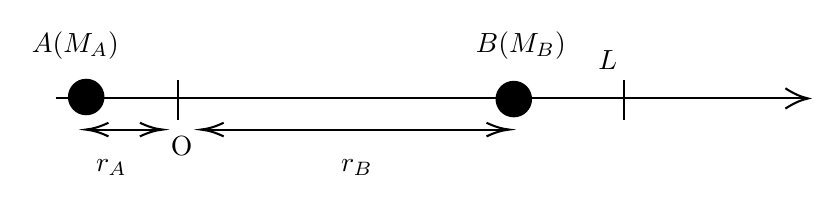
\begin{tikzpicture}[x=0.75pt,y=0.75pt,yscale=-1,xscale=1]
		%uncomment if require: \path (0,1046); %set diagram left start at 0, and has height of 1046
		
		%Straight Lines [id:da563900420095719] 
		\draw    (128,95) -- (488.5,95) ;
		\draw [shift={(490.5,95)}, rotate = 180] [color={rgb, 255:red, 0; green, 0; blue, 0 }  ][line width=0.75]    (10.93,-4.9) .. controls (6.95,-2.3) and (3.31,-0.67) .. (0,0) .. controls (3.31,0.67) and (6.95,2.3) .. (10.93,4.9)   ;
		%Straight Lines [id:da2537937486626065] 
		\draw    (187,86.1) -- (187,105.5) ;
		%Straight Lines [id:da6429853426946757] 
		\draw    (402,86.1) -- (402,105.5) ;
		%Shape: Circle [id:dp2603731885714886] 
		\draw  [fill={rgb, 255:red, 0; green, 0; blue, 0 }  ,fill opacity=1 ] (340.4,95.3) .. controls (340.4,90.72) and (344.12,87) .. (348.7,87) .. controls (353.28,87) and (357,90.72) .. (357,95.3) .. controls (357,99.88) and (353.28,103.6) .. (348.7,103.6) .. controls (344.12,103.6) and (340.4,99.88) .. (340.4,95.3) -- cycle ;
		%Shape: Circle [id:dp3731074542807482] 
		\draw  [fill={rgb, 255:red, 0; green, 0; blue, 0 }  ,fill opacity=1 ] (134.4,94.3) .. controls (134.4,89.72) and (138.12,86) .. (142.7,86) .. controls (147.28,86) and (151,89.72) .. (151,94.3) .. controls (151,98.88) and (147.28,102.6) .. (142.7,102.6) .. controls (138.12,102.6) and (134.4,98.88) .. (134.4,94.3) -- cycle ;
		%Straight Lines [id:da6647024407753024] 
		\draw    (144.5,110) -- (177.5,110) ;
		\draw [shift={(179.5,110)}, rotate = 180] [color={rgb, 255:red, 0; green, 0; blue, 0 }  ][line width=0.75]    (10.93,-3.29) .. controls (6.95,-1.4) and (3.31,-0.3) .. (0,0) .. controls (3.31,0.3) and (6.95,1.4) .. (10.93,3.29)   ;
		\draw [shift={(142.5,110)}, rotate = 0] [color={rgb, 255:red, 0; green, 0; blue, 0 }  ][line width=0.75]    (10.93,-3.29) .. controls (6.95,-1.4) and (3.31,-0.3) .. (0,0) .. controls (3.31,0.3) and (6.95,1.4) .. (10.93,3.29)   ;
		%Straight Lines [id:da15388850092552842] 
		\draw    (200,110) -- (344.5,110) ;
		\draw [shift={(346.5,110)}, rotate = 180] [color={rgb, 255:red, 0; green, 0; blue, 0 }  ][line width=0.75]    (10.93,-3.29) .. controls (6.95,-1.4) and (3.31,-0.3) .. (0,0) .. controls (3.31,0.3) and (6.95,1.4) .. (10.93,3.29)   ;
		\draw [shift={(198,110)}, rotate = 0] [color={rgb, 255:red, 0; green, 0; blue, 0 }  ][line width=0.75]    (10.93,-3.29) .. controls (6.95,-1.4) and (3.31,-0.3) .. (0,0) .. controls (3.31,0.3) and (6.95,1.4) .. (10.93,3.29)   ;
		
		% Text Node
		\draw (182,112) node [anchor=north west][inner sep=0.75pt]   [align=left] {O};
		% Text Node
		\draw (388,70.4) node [anchor=north west][inner sep=0.75pt]    {$L$};
		% Text Node
		\draw (115,61.4) node [anchor=north west][inner sep=0.75pt]    {$A( M_{A})$};
		% Text Node
		\draw (329,61.4) node [anchor=north west][inner sep=0.75pt]    {$B( M_{B})$};
		% Text Node
		\draw (146,122.9) node [anchor=north west][inner sep=0.75pt]    {$r_{A}$};
		% Text Node
		\draw (264,122.9) node [anchor=north west][inner sep=0.75pt]    {$r_{B}$};
		
		\end{tikzpicture}
		\vspace*{3mm}		
		\caption[]{Configuration to mathematically determine the position of point L2}
	\end{figure}
	and let us consider $M_A\gg M_B$ without forgetting that in this scenario $x>r_B$.

	We then have almost the same developments as for L1 but with the difference that:
	
	becomes:
	
	and that instead of having:
	
	We have:
	
	and therefore:
	
	Still with:
	
	and therefore:
	
	which corresponds to the Lagrange point L2.

	A special case again about L2 is when $M_A=M_B=M$, then $r_A=r_B=r$, then O is at the midpoint of $\overline{AB}$. Then we have:
	
	Therefore:
	
	becomes:
	
	It is no longer possible to extract the roots here (at least to my knowledge). It must be done through a numerical approximation. In Maple 4.00b, we simply put:

	\texttt{>solve(-1/(r+x)\string^2-1/(x-r)\string^2=x/(8*r\string^3),x);allvalues(");}
	
	and the only feasible solution in $\mathbb{R}$ is then $x\cong 2.8r$ and the others being in $\mathbb{C}$.
	
	\pagebreak
	\paragraph{L3 Lagrange point}\mbox{}\\\\\
	In this third sub-case, we consider:
	
	So we look for the equilibrium points beyond $A$.

	Thus we have:
	
	which becomes simply:
	
	The left side is an increasing function of $x$ from $-\infty$ to $+\infty$ when $x$ describes $]-r_A,-\infty]$. So there is a unique solution, and one equilibrium point beyond $A$. This point is denoted: L3.

	This value can be obtained by considering a limit case: when $M_B$ tends to $0$ (corresponding to a massive celestial object $A$ turning around much smaller object $B$), then $A$ tends to O, $r_A$ to 0 and therefore:
	
	with $R=\overline{AB}$. Therefore, in this limit case:
	
	becomes approximately:
	
	and therefore:
	
	So the only value of $x$ satisfying this relation will be $x=R$. The point L3 will finish to merge with the position diametrically opposite to that of $B$.

	Knowing this limit case, let us do a more detailed study now. Consider the following diagram relative to our previous limit situation:
	\begin{figure}[H]
		\centering
		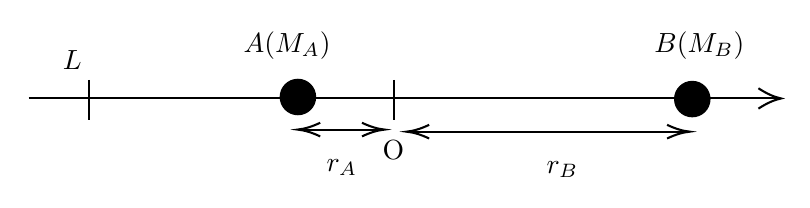
\begin{tikzpicture}[x=0.75pt,y=0.75pt,yscale=-1,xscale=1]
		%uncomment if require: \path (0,1046); %set diagram left start at 0, and has height of 1046
		
		%Straight Lines [id:da563900420095719] 
		\draw    (128,95) -- (488.5,95) ;
		\draw [shift={(490.5,95)}, rotate = 180] [color={rgb, 255:red, 0; green, 0; blue, 0 }  ][line width=0.75]    (10.93,-4.9) .. controls (6.95,-2.3) and (3.31,-0.67) .. (0,0) .. controls (3.31,0.67) and (6.95,2.3) .. (10.93,4.9)   ;
		%Straight Lines [id:da2537937486626065] 
		\draw    (304,86.1) -- (304,105.5) ;
		%Straight Lines [id:da6429853426946757] 
		\draw    (157,86.1) -- (157,105.5) ;
		%Shape: Circle [id:dp2603731885714886] 
		\draw  [fill={rgb, 255:red, 0; green, 0; blue, 0 }  ,fill opacity=1 ] (439.4,95.3) .. controls (439.4,90.72) and (443.12,87) .. (447.7,87) .. controls (452.28,87) and (456,90.72) .. (456,95.3) .. controls (456,99.88) and (452.28,103.6) .. (447.7,103.6) .. controls (443.12,103.6) and (439.4,99.88) .. (439.4,95.3) -- cycle ;
		%Shape: Circle [id:dp3731074542807482] 
		\draw  [fill={rgb, 255:red, 0; green, 0; blue, 0 }  ,fill opacity=1 ] (249.4,94.3) .. controls (249.4,89.72) and (253.12,86) .. (257.7,86) .. controls (262.28,86) and (266,89.72) .. (266,94.3) .. controls (266,98.88) and (262.28,102.6) .. (257.7,102.6) .. controls (253.12,102.6) and (249.4,98.88) .. (249.4,94.3) -- cycle ;
		%Straight Lines [id:da6647024407753024] 
		\draw    (259.5,110) -- (297.5,110) ;
		\draw [shift={(299.5,110)}, rotate = 180] [color={rgb, 255:red, 0; green, 0; blue, 0 }  ][line width=0.75]    (10.93,-3.29) .. controls (6.95,-1.4) and (3.31,-0.3) .. (0,0) .. controls (3.31,0.3) and (6.95,1.4) .. (10.93,3.29)   ;
		\draw [shift={(257.5,110)}, rotate = 0] [color={rgb, 255:red, 0; green, 0; blue, 0 }  ][line width=0.75]    (10.93,-3.29) .. controls (6.95,-1.4) and (3.31,-0.3) .. (0,0) .. controls (3.31,0.3) and (6.95,1.4) .. (10.93,3.29)   ;
		%Straight Lines [id:da15388850092552842] 
		\draw    (312,111) -- (444.5,111) ;
		\draw [shift={(446.5,111)}, rotate = 180] [color={rgb, 255:red, 0; green, 0; blue, 0 }  ][line width=0.75]    (10.93,-3.29) .. controls (6.95,-1.4) and (3.31,-0.3) .. (0,0) .. controls (3.31,0.3) and (6.95,1.4) .. (10.93,3.29)   ;
		\draw [shift={(310,111)}, rotate = 0] [color={rgb, 255:red, 0; green, 0; blue, 0 }  ][line width=0.75]    (10.93,-3.29) .. controls (6.95,-1.4) and (3.31,-0.3) .. (0,0) .. controls (3.31,0.3) and (6.95,1.4) .. (10.93,3.29)   ;
		
		% Text Node
		\draw (297,114) node [anchor=north west][inner sep=0.75pt]   [align=left] {O};
		% Text Node
		\draw (143,70.4) node [anchor=north west][inner sep=0.75pt]    {$L$};
		% Text Node
		\draw (230,61.4) node [anchor=north west][inner sep=0.75pt]    {$A( M_{A})$};
		% Text Node
		\draw (428,61.4) node [anchor=north west][inner sep=0.75pt]    {$B( M_{B})$};
		% Text Node
		\draw (270,122.9) node [anchor=north west][inner sep=0.75pt]    {$r_{A}$};
		% Text Node
		\draw (376,123.9) node [anchor=north west][inner sep=0.75pt]    {$r_{B}$};
		
		\end{tikzpicture}
		\vspace*{3mm}		
		\caption[]{Configuration to mathematically determine the position of point L3}
	\end{figure}
	and let us still consider $M_A \gg M_B$ without forgetting that in this scenario $x<-r_A$.

	We will first consider the following approximation:
	
	and this one also (since $\overline{\text{O}A}$ tends to zero as the celestial object $A$ becomes very massive):
	
	Since then:
	
	We have also (...):
	
	when at the limit where the celestial object $A$ is really massive, we fall back on the first term ...

	With the last two relations, we have:
	
	if we neglect the terms of the second order.

	Furthermore, we have also:
	
	Let us recall the equilibrium condition:
	
	And let us put everything we got until now inside it:
	
	What becomes after simplifications:
	
	after a small approximation:
	
	after simplification:
	
	Hence:
	
	and finally:
	
	\begin{tcolorbox}[title=Remark,arc=10pt,breakable,drop lifted shadow,
  skin=enhanced,
  skin first is subskin of={enhancedfirst}{arc=10pt,no shadow},
  skin middle is subskin of={enhancedmiddle}{arc=10pt,no shadow},
  skin last is subskin of={enhancedlast}{drop lifted shadow}]
	For some Si-Fi authors, for reminder... this L3 point opposite to the Earth relatively to the Sun would hide us a hypothetical planet that would be forever hidden to us by the Sun..........
	\end{tcolorbox}
	
	\subsubsection{Equilibrium points of the second type}
	The equilibrium positions of the second type are those for which $y\neq 0$. In other words the points outside of the line $\overline{AB}$, but still in the plane $\text{O}xy$.

	Thus, our system of equations remains:
	
	
	\paragraph{L4, L5 Lagrange points}\mbox{}\\\\\
	To determine the remaining equilibrium points, we can divide the second equation of the system such that the latter becomes:
	
	\begin{figure}[H]
		\centering
		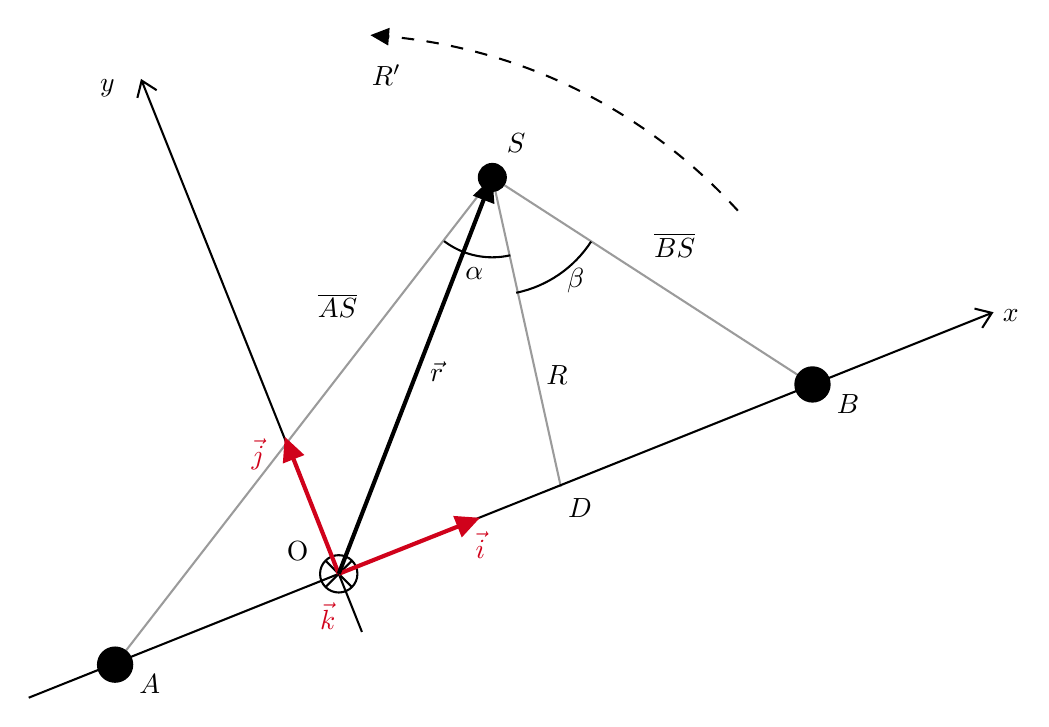
\begin{tikzpicture}[x=0.75pt,y=0.75pt,yscale=-1,xscale=1]
		%uncomment if require: \path (0,1215); %set diagram left start at 0, and has height of 1215
		
		%Straight Lines [id:da033559841981090965] 
		\draw [color={rgb, 255:red, 155; green, 155; blue, 155 }  ,draw opacity=1 ]   (363.5,260) -- (330.5,111) ;
		%Straight Lines [id:da062449330362460254] 
		\draw [color={rgb, 255:red, 155; green, 155; blue, 155 }  ,draw opacity=1 ]   (484.75,210.75) -- (330.5,111) ;
		%Straight Lines [id:da44257618491226136] 
		\draw [color={rgb, 255:red, 155; green, 155; blue, 155 }  ,draw opacity=1 ]   (148.75,345.75) -- (330.5,111) ;
		%Shape: Axis 2D [id:dp1834894618059113] 
		\draw  (107.13,361.69) -- (571.17,176.27)(161.54,64.34) -- (267.68,329.99) (562.81,174.22) -- (571.17,176.27) -- (566.52,183.51) (159.49,72.69) -- (161.54,64.34) -- (168.78,68.98)  ;
		%Flowchart: Summing Junction [id:dp895245393415119] 
		\draw   (247.5,302) .. controls (247.5,297.03) and (251.53,293) .. (256.5,293) .. controls (261.47,293) and (265.5,297.03) .. (265.5,302) .. controls (265.5,306.97) and (261.47,311) .. (256.5,311) .. controls (251.53,311) and (247.5,306.97) .. (247.5,302) -- cycle ; \draw   (250.14,295.64) -- (262.86,308.36) ; \draw   (262.86,295.64) -- (250.14,308.36) ;
		%Straight Lines [id:da9523460776933002] 
		\draw [color={rgb, 255:red, 208; green, 2; blue, 27 }  ,draw opacity=1 ][line width=1.5]    (256.5,302) -- (231.97,239.72) ;
		\draw [shift={(230.5,236)}, rotate = 68.5] [fill={rgb, 255:red, 208; green, 2; blue, 27 }  ,fill opacity=1 ][line width=0.08]  [draw opacity=0] (11.61,-5.58) -- (0,0) -- (11.61,5.58) -- cycle    ;
		%Straight Lines [id:da4672352117535321] 
		\draw [color={rgb, 255:red, 208; green, 2; blue, 27 }  ,draw opacity=1 ][line width=1.5]    (256.5,302) -- (320.78,276.48) ;
		\draw [shift={(324.5,275)}, rotate = 158.34] [fill={rgb, 255:red, 208; green, 2; blue, 27 }  ,fill opacity=1 ][line width=0.08]  [draw opacity=0] (11.61,-5.58) -- (0,0) -- (11.61,5.58) -- cycle    ;
		%Straight Lines [id:da35782354736011945] 
		\draw [color={rgb, 255:red, 0; green, 0; blue, 0 }  ,draw opacity=1 ][line width=1.5]    (256.5,302) -- (329.05,114.73) ;
		\draw [shift={(330.5,111)}, rotate = 111.18] [fill={rgb, 255:red, 0; green, 0; blue, 0 }  ,fill opacity=1 ][line width=0.08]  [draw opacity=0] (11.61,-5.58) -- (0,0) -- (11.61,5.58) -- cycle    ;
		%Shape: Circle [id:dp595066926449888] 
		\draw  [fill={rgb, 255:red, 0; green, 0; blue, 0 }  ,fill opacity=1 ] (324,111) .. controls (324,107.41) and (326.91,104.5) .. (330.5,104.5) .. controls (334.09,104.5) and (337,107.41) .. (337,111) .. controls (337,114.59) and (334.09,117.5) .. (330.5,117.5) .. controls (326.91,117.5) and (324,114.59) .. (324,111) -- cycle ;
		%Shape: Circle [id:dp7765048303145505] 
		\draw  [fill={rgb, 255:red, 0; green, 0; blue, 0 }  ,fill opacity=1 ] (476.5,210.75) .. controls (476.5,206.19) and (480.19,202.5) .. (484.75,202.5) .. controls (489.31,202.5) and (493,206.19) .. (493,210.75) .. controls (493,215.31) and (489.31,219) .. (484.75,219) .. controls (480.19,219) and (476.5,215.31) .. (476.5,210.75) -- cycle ;
		%Shape: Circle [id:dp5381019368944424] 
		\draw  [fill={rgb, 255:red, 0; green, 0; blue, 0 }  ,fill opacity=1 ] (140.5,345.75) .. controls (140.5,341.19) and (144.19,337.5) .. (148.75,337.5) .. controls (153.31,337.5) and (157,341.19) .. (157,345.75) .. controls (157,350.31) and (153.31,354) .. (148.75,354) .. controls (144.19,354) and (140.5,350.31) .. (140.5,345.75) -- cycle ;
		%Shape: Arc [id:dp6688141164231127] 
		\draw  [draw opacity=0][dash pattern={on 4.5pt off 4.5pt}] (271.78,42.46) .. controls (342.09,46.54) and (404.9,78.55) .. (449.28,127.57) -- (256.5,302) -- cycle ; \draw [dash pattern={on 4.5pt off 4.5pt}] [dash pattern={on 4.5pt off 4.5pt}]  (274.94,42.67) .. controls (343.97,47.5) and (405.56,79.29) .. (449.28,127.57) ;  \draw [shift={(271.78,42.46)}, rotate = 4.7] [fill={rgb, 255:red, 0; green, 0; blue, 0 }  ][dash pattern={on 3.49pt off 4.5pt}][line width=0.08]  [draw opacity=0] (8.93,-4.29) -- (0,0) -- (8.93,4.29) -- cycle    ;
		%Shape: Arc [id:dp894707174023031] 
		\draw  [draw opacity=0] (339.16,148.52) .. controls (336.37,149.16) and (333.48,149.5) .. (330.5,149.5) .. controls (321.76,149.5) and (313.71,146.59) .. (307.25,141.69) -- (330.5,111) -- cycle ; \draw   (339.16,148.52) .. controls (336.37,149.16) and (333.48,149.5) .. (330.5,149.5) .. controls (321.76,149.5) and (313.71,146.59) .. (307.25,141.69) ;  
		%Shape: Arc [id:dp7720850245133084] 
		\draw  [draw opacity=0] (378.09,141.93) .. controls (369.97,154.4) and (357.08,163.48) .. (342,166.58) -- (330.5,111) -- cycle ; \draw   (378.09,141.93) .. controls (369.97,154.4) and (357.08,163.48) .. (342,166.58) ;  
		
		% Text Node
		\draw (140,62.4) node [anchor=north west][inner sep=0.75pt]    {$y$};
		% Text Node
		\draw (575,173.4) node [anchor=north west][inner sep=0.75pt]    {$x$};
		% Text Node
		\draw (230,285) node [anchor=north west][inner sep=0.75pt]   [align=left] {O};
		% Text Node
		\draw (213,235.4) node [anchor=north west][inner sep=0.75pt]  [color={rgb, 255:red, 208; green, 2; blue, 27 }  ,opacity=1 ]  {$\vec{j}$};
		% Text Node
		\draw (321,280.4) node [anchor=north west][inner sep=0.75pt]  [color={rgb, 255:red, 208; green, 2; blue, 27 }  ,opacity=1 ]  {$\vec{i}$};
		% Text Node
		\draw (246,314.4) node [anchor=north west][inner sep=0.75pt]  [color={rgb, 255:red, 208; green, 2; blue, 27 }  ,opacity=1 ]  {$\vec{k}$};
		% Text Node
		\draw (336,88.4) node [anchor=north west][inner sep=0.75pt]    {$S$};
		% Text Node
		\draw (299,198.4) node [anchor=north west][inner sep=0.75pt]    {$\vec{r}$};
		% Text Node
		\draw (159,349.15) node [anchor=north west][inner sep=0.75pt]    {$A$};
		% Text Node
		\draw (495,214.15) node [anchor=north west][inner sep=0.75pt]    {$B$};
		% Text Node
		\draw (271,55.4) node [anchor=north west][inner sep=0.75pt]    {$R'$};
		% Text Node
		\draw (365.5,264.4) node [anchor=north west][inner sep=0.75pt]    {$D$};
		% Text Node
		\draw (407,136.4) node [anchor=north west][inner sep=0.75pt]    {$\overline{BS}$};
		% Text Node
		\draw (245,165.4) node [anchor=north west][inner sep=0.75pt]    {$\overline{AS}$};
		% Text Node
		\draw (355,200.4) node [anchor=north west][inner sep=0.75pt]    {$R$};
		% Text Node
		\draw (316,153) node [anchor=north west][inner sep=0.75pt]    {$\alpha $};
		% Text Node
		\draw (365,153.4) node [anchor=north west][inner sep=0.75pt]    {$\beta $};
		\end{tikzpicture}
		\vspace*{3mm}
		\caption[]{Configuration to mathematically determine the position of points L4,L5}
	\end{figure}
	where $\overline{AB}$ is obviously the distance between $A$ and $B$ and $D$ is the centroid of the system given by (\SeeChapter{see section Classical Mechanics page \pageref{center of mass}}):
	
	which are the radii of gyration of the bodies $A$ and $B$.

	It is easy to verify that the sum of both previous distances is equal to $\overline{AB}$ and their proportion $M_B/M_A$. Another form of $\overline{DB}$ (which will be useful) is obtained by dividing the numerator and denominator by $M_A$:
	
	We know according to our previous calculations that $\overline{AS}=\overline{BS}$ but this is insufficient. We still want to know the angles of the vertices $A$, $B$, $S$, and this is what we will look for now.

	In this context, if a satellite $S$ is in equilibrium, there will always remain at the same distance of $A$ or $B$. The center of rotation of the $3$ points is the point $D$, the mass $A$ itself revolves around it. If the satellite, $S$, remains stable, the three bodies have the same orbital period $T$. If $S$ is immobile in this frame in rotation it will not be subject to the Coriolis force but only to centrifugal force of $A$ and of $B$.
	
	Let us denote by $v_B$ the rotation speed of $B$ and $v_S$ the rotation speed of $S$. Then we have:
	
	and:
	
	From whose we get that:
	
	and:
	
	So we can equate these two expressions:
	
	This merely expresses the well known fact that if two objects rotate together, the furthest one from the centroid is the fastest. Speeds are proportional to the distances from the centroid.

	The centrifugal force on $B$ is in equilibrium with the gravitational force of $A$ and it is expressed by:
	
	Thus by simplifying:
	
	Similarly, the centrifugal force applied on $S$ is:
	
	It is balanced by the forces of attraction $\vec{F}_A$,$\vec{F}_B$ of the objects $A$ and $B$. However, only the components of these forces located on the line $R$ oppose efficiently to this centrifugal force. Hence:
	
	
	and as:
	
	We then have:
	
	In addition, the forces applied to $S$ and perpendicular to $R$ must vanish. If not, the object $S$ would follow the largest mass and would not remain in position and would therefore no longer be in equilibrium. We must then have:
	
	Or, after substitution and simplification:
	
	Of all the equations obtained up to now the only that bother us are those containing both speeds and angles $\alpha$,$\beta$. This requires that we must arrive to eliminate what is convenient to have only the last two parameters (that is to say: the angles).

	For this, we take the square:
	
	We multiply both sides by $\overline{AB}^2$ and we divide by $1+\dfrac{M_B}{M_A}$:
	
	which is similar to:
	
	Thus equating:
	
	So we removed the speed of $B$. Now, let us multiply both sides by $\left(1+\dfrac{M_B}{M_A}\right)R$ and divide by $\overline{AB}^2$:
	
	which is similar to:
	
	Therefore:
	
	By dividing the whole by $GM_A$ we find:
	
	And as we have proved at the beginning $\overline{AS}=\overline{BS}$ that we will denote by $R'$, then we have:
	
	and let us recall that we have:
	
	Therefore:
	
	This allows us to write:
	
	And multiplying by $\sin(\beta)$:
	
	We can now notice a thing (not easy to see...). If $R'=\overline{AB}$ (that is that the triangle $ABS$ is equilateral) the previous relations simplifies to:
	
	But, if the triangle is really equilateral, then we have (\SeeChapter{see section Geometric Shapes page \pageref{lateral triangle}}):
	
	Hence:
	
	What can finally write:
	
	Which is just the sine theorem for the triangle $SDB$ (\SeeChapter{see section Trigonometry page \pageref{law of sines}}) and is therefore certain. Returning back, we can now prove that all previous equations are satisfied if and only if $ABS$ is equilateral. If we had not put $ABS$ as equilateral, we would have gotten a different relation of the sine theorem, without possible verification, and the set of equations required for equilibrium at the point $S$ could not be met.

	Conclusion of the thing ... the system gives as a solution:
	
	$ABS$ (or $ABL$ regardless the notation), then forms an equilateral triangle. The two equilibrium points are denoted L4 and L5. L4 is located in advance with respect to the less massive celestial object and L5 is late relatively to it.
	\begin{figure}[H]
		\centering
		\begin{tikzpicture}[x=0.75pt,y=0.75pt,yscale=-1,xscale=1]
		%uncomment if require: \path (0,1046); %set diagram left start at 0, and has height of 1046
		
		%Straight Lines [id:da563900420095719] 
		\draw    (128,95) -- (488.5,95) ;
		\draw [shift={(490.5,95)}, rotate = 180] [color={rgb, 255:red, 0; green, 0; blue, 0 }  ][line width=0.75]    (10.93,-4.9) .. controls (6.95,-2.3) and (3.31,-0.67) .. (0,0) .. controls (3.31,0.67) and (6.95,2.3) .. (10.93,4.9)   ;
		%Straight Lines [id:da2537937486626065] 
		\draw    (189,86.1) -- (189,105.5) ;
		%Shape: Circle [id:dp2603731885714886] 
		\draw  [fill={rgb, 255:red, 0; green, 0; blue, 0 }  ,fill opacity=1 ] (439.4,95.3) .. controls (439.4,90.72) and (443.12,87) .. (447.7,87) .. controls (452.28,87) and (456,90.72) .. (456,95.3) .. controls (456,99.88) and (452.28,103.6) .. (447.7,103.6) .. controls (443.12,103.6) and (439.4,99.88) .. (439.4,95.3) -- cycle ;
		%Shape: Circle [id:dp3731074542807482] 
		\draw  [fill={rgb, 255:red, 0; green, 0; blue, 0 }  ,fill opacity=1 ] (134.4,94.3) .. controls (134.4,89.72) and (138.12,86) .. (142.7,86) .. controls (147.28,86) and (151,89.72) .. (151,94.3) .. controls (151,98.88) and (147.28,102.6) .. (142.7,102.6) .. controls (138.12,102.6) and (134.4,98.88) .. (134.4,94.3) -- cycle ;
		%Straight Lines [id:da6647024407753024] 
		\draw    (144.5,110) -- (182.5,110) ;
		\draw [shift={(184.5,110)}, rotate = 180] [color={rgb, 255:red, 0; green, 0; blue, 0 }  ][line width=0.75]    (10.93,-3.29) .. controls (6.95,-1.4) and (3.31,-0.3) .. (0,0) .. controls (3.31,0.3) and (6.95,1.4) .. (10.93,3.29)   ;
		\draw [shift={(142.5,110)}, rotate = 0] [color={rgb, 255:red, 0; green, 0; blue, 0 }  ][line width=0.75]    (10.93,-3.29) .. controls (6.95,-1.4) and (3.31,-0.3) .. (0,0) .. controls (3.31,0.3) and (6.95,1.4) .. (10.93,3.29)   ;
		%Straight Lines [id:da15388850092552842] 
		\draw    (199,111) -- (442.5,111) ;
		\draw [shift={(444.5,111)}, rotate = 180] [color={rgb, 255:red, 0; green, 0; blue, 0 }  ][line width=0.75]    (10.93,-3.29) .. controls (6.95,-1.4) and (3.31,-0.3) .. (0,0) .. controls (3.31,0.3) and (6.95,1.4) .. (10.93,3.29)   ;
		\draw [shift={(197,111)}, rotate = 0] [color={rgb, 255:red, 0; green, 0; blue, 0 }  ][line width=0.75]    (10.93,-3.29) .. controls (6.95,-1.4) and (3.31,-0.3) .. (0,0) .. controls (3.31,0.3) and (6.95,1.4) .. (10.93,3.29)   ;
		\draw   (293.5,189.8) -- (307.1,189.8)(300.3,183) -- (300.3,196.6) ;
		\draw   (293.5,23.8) -- (307.1,23.8)(300.3,17) -- (300.3,30.6) ;
		
		% Text Node
		\draw (182,112) node [anchor=north west][inner sep=0.75pt]   [align=left] {O};
		% Text Node
		\draw (279,194.4) node [anchor=north west][inner sep=0.75pt]    {$L$};
		% Text Node
		\draw (115,61.4) node [anchor=north west][inner sep=0.75pt]    {$A( M_{A})$};
		% Text Node
		\draw (428,61.4) node [anchor=north west][inner sep=0.75pt]    {$B( M_{B})$};
		% Text Node
		\draw (154,122.9) node [anchor=north west][inner sep=0.75pt]    {$r_{A}$};
		% Text Node
		\draw (318,123.9) node [anchor=north west][inner sep=0.75pt]    {$r_{B}$};
		% Text Node
		\draw (279,5.4) node [anchor=north west][inner sep=0.75pt]    {$L$};
		
		\end{tikzpicture}
		\vspace*{3mm}
		\caption[]{L4 and L5 equilateral triangle}
	\end{figure}
	In the year 12000 (holocene calendar), $385$ asteroids in the L4 point and $188$ asteroids in the L5 point were counted on the orbit of Jupiter, but located precisely in an equilateral triangle with the Sun and Jupiter either side of Jupiter: these are the Trojan planets. It was also observed two objects at the point L5 of Mars discovered in 11990 and 11998 (holocene calendar).
	
	\pagebreak
	\subsection{Relativistic Doppler-Fizeau Effect}\label{relativitic doppler-fizeau effect}
	The Doppler effect is the difference between the frequency of the transmitted wave and the received wave when the transmitter and receiver are moving relative to each other (\SeeChapter{see section Music Mathematics page \pageref{acoustic doppler effect}}). This is an effect that must be take into account astronomy to calculate the distance of the body assuming its known (or estimated)  emission wavelength and measuring its received wavelength or for measuring the speed of rotation (radial velocity) of stars by observing very precisely and successively their opposite edges and measuring the shift of the spectrum obtained.

	In the early 121st century (holocene calendar) the precision and finesse of the spectra of measures has reached a level that allows to observe even minimal changes in the distance of stars and so speculate on possible planetary satellites (this may work if the plane of the orbit passes through the Earth):
	\begin{figure}[H]
		\centering
		\includegraphics[scale=0.8]{img/cosmology/doppler_effect_radial_velocity.jpg}
		\caption[Doppler-Effect radial velocity method]{Doppler-Effect radial velocity method (source: ESO Press Photo 22e/05 12007-04-11)}
	\end{figure}
	The Doppler effect of electromagnetic waves must be discussed independently of the acoustic Doppler effect (also named "Galilean Doppler effect") studied in the section of Music Mathematics (see page \pageref{acoustic doppler effect}). First, because the electromagnetic waves do not consist of a material movement and therefore the speed of the source relative to the medium does not enter into the discussion, then because their velocity is $c$ (the speed of light) and remains the same for all observers independently of their relative movements. The Doppler effect for electromagnetic waves is thus calculated necessarily using the principle of relativity and is symmetrical with respect to relative movement of the source and the observer (as opposed to acoustic cases).
	
	For an observer in an inertial reference frame, a plane and harmonic electromagnetic wave can be described by a function of the form:
	
	multiplied by an appropriate amplitude factor. For an observer attached to another inertial frame, the components $x$ and $t$ should be replaced with $x'$ and $t'$, obtained by the Lorentz transformation (\SeeChapter{see section Special Relativity page \pageref{lorentz transformations}}), and that latter will therefore write to describing plane wave:
	
	where $k'$ and $\omega'$ are not necessarily the same as that of the another observer (precisely this is what we want to determine). Moreover, the principle of relativity has allowed us to demonstrate in the section of Special Relativity that:
	
	This assumes that the expression:
	
	remains invariant when we move from one inertial observer to the other. We then have:
	
	Using the Lorentz transformation relations (\SeeChapter{see section Special Relativity page \pageref{lorentz transformations}}), we have immediately:
	
	Hence:
	
	Grouping we get:
	
	By identification, it comes immediately:
	
	If we consider that:
	
	in the case of electromagnetic waves, we can write each of these relation in the form:
	
	The ratio visible in the both expression above is named the "\NewTerm{radial relativistic doppler redshift}\index{redshift!radial relativistic doppler redshift}" and is denoted by:
	
	for a movement of the observer relative to the source in the direction of propagation (the range of this function is bounded to $[0,1]$). In the other case (opposite direction) we have obviously:
	
	That is unbounded and has for range $[1,+\infty[$. Physicists like to normalized stuffs so that the range is $[0,+\infty[$, so we write and define the "\NewTerm{relativistic doppler redshift}" for opposite direction as:
	
	Or more commonly written as:
	
	
	\begin{figure}[H]
		\centering
		\includegraphics[width=\textwidth]{img/cosmology/hubble_deep_space_redshift.jpg}
		\caption[High-redshift galaxy candidates in the Hubble ultra deep field]{High-redshift galaxy candidates in the Hubble ultra deep field 12012 (source: NASA, ESA, R. Ellis (Caltech), and the HUDF Team)}
	\end{figure}
	
	\begin{figure}[H]
		\centering
		\includegraphics[width=\textwidth]{img/cosmology/jswt_deep_space_redshift.jpg}
		\caption[James Webb Telescope galaxy cluster SMACS 0723 deep field]{James Webb Telescope galaxy cluster SMACS 0723 deep field released in 12022, July 11 (source: NASA)}
	\end{figure}
	Obviously if the source or observer don't move away but approach then we not have a red shift but a "\NewTerm{blueshift}\index{blueshift}".
	
	Furthermore, the last relation with the pulsations is most often written in the literature as follows:
	
	Which is written most often in the following form (keep in mind that this is in the case when the two referential move in opposite direction!):
	
	Therefore if we measure the both frequencies (supposing that we know what should be the source), then we can also obviously determine the speed $v$ of the observed object.
	
	Or in case of wavelength we have similarly:
	
	
	When a spectrum can be obtained, determining the red shift is rather straight-forward: if you can localize the spectral fingerprint of a common element, such as hydrogen, then the red shift can be computed using simple arithmetic. But similarly to the case of star/quasar classification, the task becomes much more difficult when only photometric observations are available:
	\begin{figure}[H]
		\centering
		\includegraphics[scale=0.8]{img/cosmology/red_shift_spectrum.jpg}
	\end{figure}
	It must be recalled that the pulsation offset (and therefore frequency offset) that takes place here is due to a relative motion of the observer with respect to the source and not to something else (or respectively of the source relatively to the observer). Indeed, in our study of General Relativity (\SeeChapter{see section General Relativity page \pageref{shapiro effect}}), we will prove that there is a superposition of a shift because of the gravitational field surrounding the emitter that will be considered as caused by the space-time curvature.

	Finally, for sceptics who want to check in another way that the Doppler phenomenon is well symmetric unlike the acoustic Doppler effect proved in the section of Music Mathematics, here's another approach:

	First, consider that it is the source moving away. If we calculated by the classical relation proved in the section of Music Mathematics the frequency of the signal at the reception would be (see page \pageref{acoustic doppler effect}):
	
	and we must take into account the time dilation for $f$ with (\SeeChapter{see section Special Relativity page \pageref{relativistic time variation}}):
	
	because the time interval of the fixed observer is longer than that of the source (time is faster for observer at rest).

	It comes then:
	
	and if it is the observer who moves away from the source we proved in the section of Music Mathematics that:
	
	both relations are indeed symmetric in the special relativistic case (as expected for electrodynamics)!
	\begin{tcolorbox}[title=Remark,arc=10pt,breakable,drop lifted shadow,
  skin=enhanced,
  skin first is subskin of={enhancedfirst}{arc=10pt,no shadow},
  skin middle is subskin of={enhancedmiddle}{arc=10pt,no shadow},
  skin last is subskin of={enhancedlast}{drop lifted shadow}]
	Currently, astronomers have courses in astrophysics and their observations are generally studied in an astrophysical context, so there is less distinction between the two disciplines than before.
	\end{tcolorbox}
	A very good example of the application of the Doppler effect is to explore the limits given by measuring the apparent speed. Let's see what it is:
	
	\subsubsection{Apparent speed}
	By measuring the apparent speed of movement of very fast objects in the sky (plasma jets, etc.), astrophysicists have obtained apparent displacement speeds exceeding the speed of light in vacuum!

	In fact, it is an illusion that can occur if the speed of the object is very close to that of light it emits, so close enough to $c$.
	\begin{figure}[H]
		\centering
		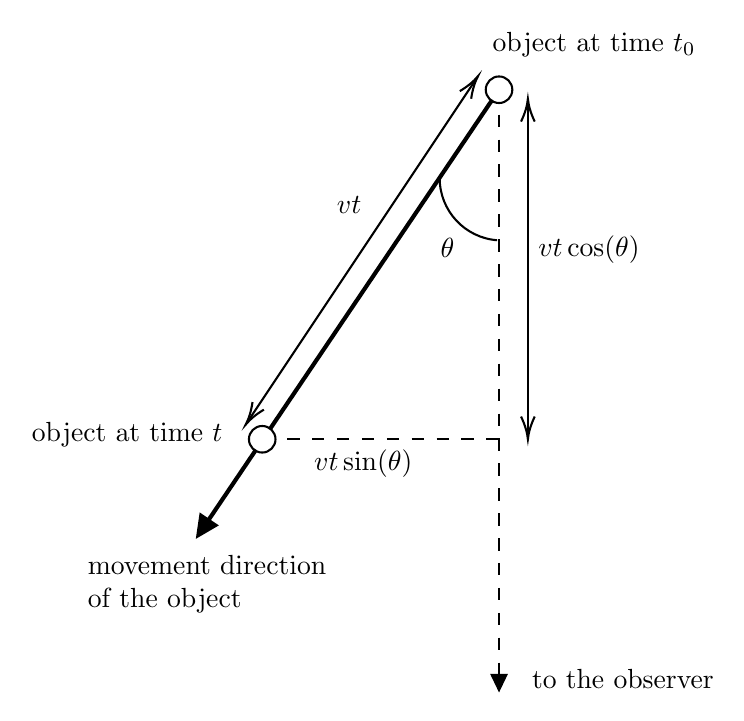
\begin{tikzpicture}[x=0.75pt,y=0.75pt,yscale=-1,xscale=1]
		%uncomment if require: \path (0,1046); %set diagram left start at 0, and has height of 1046
		
		%Straight Lines [id:da554022000631134] 
		\draw  [dash pattern={on 4.5pt off 4.5pt}]  (352.6,47.4) -- (352.6,334.8) ;
		\draw [shift={(352.6,337.8)}, rotate = 270] [fill={rgb, 255:red, 0; green, 0; blue, 0 }  ][line width=0.08]  [draw opacity=0] (8.93,-4.29) -- (0,0) -- (8.93,4.29) -- cycle    ;
		%Straight Lines [id:da06325627925381849] 
		\draw [line width=1.5]    (352.6,47.4) -- (208.74,260.48) ;
		\draw [shift={(206.5,263.8)}, rotate = 304.02] [fill={rgb, 255:red, 0; green, 0; blue, 0 }  ][line width=0.08]  [draw opacity=0] (11.61,-5.58) -- (0,0) -- (11.61,5.58) -- cycle    ;
		%Straight Lines [id:da8866025390549643] 
		\draw  [dash pattern={on 4.5pt off 4.5pt}]  (238.5,215.8) -- (352.5,215.8) ;
		%Straight Lines [id:da9474474103920716] 
		\draw    (366.5,53.8) -- (366.5,213.8) ;
		\draw [shift={(366.5,215.8)}, rotate = 270] [color={rgb, 255:red, 0; green, 0; blue, 0 }  ][line width=0.75]    (10.93,-3.29) .. controls (6.95,-1.4) and (3.31,-0.3) .. (0,0) .. controls (3.31,0.3) and (6.95,1.4) .. (10.93,3.29)   ;
		\draw [shift={(366.5,51.8)}, rotate = 90] [color={rgb, 255:red, 0; green, 0; blue, 0 }  ][line width=0.75]    (10.93,-3.29) .. controls (6.95,-1.4) and (3.31,-0.3) .. (0,0) .. controls (3.31,0.3) and (6.95,1.4) .. (10.93,3.29)   ;
		%Shape: Arc [id:dp740363045380195] 
		\draw  [draw opacity=0] (351.65,119.91) .. controls (336.18,118.71) and (324,105.78) .. (324,90) .. controls (324,89.93) and (324,89.85) .. (324,89.78) -- (354,90) -- cycle ; \draw   (351.65,119.91) .. controls (336.18,118.71) and (324,105.78) .. (324,90) .. controls (324,89.93) and (324,89.85) .. (324,89.78) ;  
		%Straight Lines [id:da05372032674847693] 
		\draw    (341.39,42.46) -- (231.61,207.14) ;
		\draw [shift={(230.5,208.8)}, rotate = 303.69] [color={rgb, 255:red, 0; green, 0; blue, 0 }  ][line width=0.75]    (10.93,-3.29) .. controls (6.95,-1.4) and (3.31,-0.3) .. (0,0) .. controls (3.31,0.3) and (6.95,1.4) .. (10.93,3.29)   ;
		\draw [shift={(342.5,40.8)}, rotate = 123.69] [color={rgb, 255:red, 0; green, 0; blue, 0 }  ][line width=0.75]    (10.93,-3.29) .. controls (6.95,-1.4) and (3.31,-0.3) .. (0,0) .. controls (3.31,0.3) and (6.95,1.4) .. (10.93,3.29)   ;
		%Shape: Circle [id:dp3214966801594772] 
		\draw  [fill={rgb, 255:red, 255; green, 255; blue, 255 }  ,fill opacity=1 ] (346.2,47.4) .. controls (346.2,43.87) and (349.07,41) .. (352.6,41) .. controls (356.13,41) and (359,43.87) .. (359,47.4) .. controls (359,50.93) and (356.13,53.8) .. (352.6,53.8) .. controls (349.07,53.8) and (346.2,50.93) .. (346.2,47.4) -- cycle ;
		%Shape: Circle [id:dp9635019774664242] 
		\draw  [fill={rgb, 255:red, 255; green, 255; blue, 255 }  ,fill opacity=1 ] (232.1,215.8) .. controls (232.1,212.27) and (234.97,209.4) .. (238.5,209.4) .. controls (242.03,209.4) and (244.9,212.27) .. (244.9,215.8) .. controls (244.9,219.33) and (242.03,222.2) .. (238.5,222.2) .. controls (234.97,222.2) and (232.1,219.33) .. (232.1,215.8) -- cycle ;
		
		% Text Node
		\draw (348,18) node [anchor=north west][inner sep=0.75pt]   [align=left] {object at time $\displaystyle t_{0}$};
		% Text Node
		\draw (367,325) node [anchor=north west][inner sep=0.75pt]   [align=left] {to the observer};
		% Text Node
		\draw (262,219.4) node [anchor=north west][inner sep=0.75pt]    {$vt\sin( \theta )$};
		% Text Node
		\draw (370,116.4) node [anchor=north west][inner sep=0.75pt]    {$vt\cos( \theta )$};
		% Text Node
		\draw (323,117.4) node [anchor=north west][inner sep=0.75pt]    {$\theta $};
		% Text Node
		\draw (273,97.4) node [anchor=north west][inner sep=0.75pt]    {$vt$};
		% Text Node
		\draw (126,206) node [anchor=north west][inner sep=0.75pt]   [align=left] {object at time $\displaystyle t$};
		% Text Node
		\draw (153,270) node [anchor=north west][inner sep=0.75pt]   [align=left] {movement direction\\of the object};
		
		\end{tikzpicture}
		\vspace*{3mm}	
		\caption{Schematic idea behind the apparent speed}
	\end{figure}
	The object emits light at time $t_0$, it does not instantly reach us but must travel a distance to get to us. We get it after the time:
	
	The object itself, moves with velocity $v$ at an angle $\theta$ with the viewing direction, so at time $t$, the object moved of a distance $vt$. The light emitted by the object at time $t$ must travel the distance (application of Pythagoras theorem):
	
	to reach us (the object has moved of a distance $vt\cos(\theta)$ in the direction of observation but moved away from the axis of observation of the distance $vt\sin(\theta)$), so we receive light that was emitted by the object at time $t$ after a time $t_2$:
	
	Between the two positions of the object, it has elapsed the time $t$ but, viewed from the observer, the time interval between the reception of images of these two positions is:
	
	different from $t$!
	
	For a small time interval $t$, we have, by doing a limited Taylor development:
	
	During this time interval, always from the point of view of the observer, the object appears to have moved on the sky plane by a distance of $vt\sin(\theta)$.

	Thus, the apparent speed of the object is:
	
	If we set the angle $\theta$ as being very close to a right angle, then we have the second term of the denominator that is very small which allows us with a Taylor expansion to write a relation that can be found quit often in high-school textbooks :
	
	Let us seek the maximum of this function to understand how such observation is possible by deriving relatively to $\theta$ and by seeking for what value the derivative is zero:
	
	and this vanishes after simplification of the denominator for:
	
	Hence:
	
	The apparent velocity is then:
	
	and is equal to or greater than $c$ if:
	
	Therefore:
	
	Thus we see that it is possible to observe apparent movements faster than light, even though the subject is very fast indeed, but slower than $c$. As it is only an "illusion", there is no contradiction with the theory of relativity.

	Knowing the speed of movement of a celestial object obtained using the Doppler effect and the apparent speed with the observations, it is easy for astrophysicists to determine the angle  $\theta$ by doing a little bit elementary algebra from the following relation:
	
	
	\begin{flushright}
	\begin{tabular}{l c}
	\circled{80} & \pbox{20cm}{\score{3}{5} \\ {\tiny 47 votes,  64.68\%}} 
	\end{tabular} 
	\end{flushright}
	
	%to make section start on odd page
	\newpage
	\thispagestyle{empty}
	\mbox{}
	\section{Astrophysics}\label{astrophysics}
	\lettrine[lines=4]{\color{BrickRed}A}{strophysics} is an interdisciplinary branch of astronomy which mainly concerns physics and the study of the properties of objects in the Universe (stars, planets, galaxies, interstellar medium for examples) as their luminosity, density, temperature and their chemical composition. The first scientific approaches in this area date from the early 119th century (holocene calendar).
	
	\begin{fquote}[Carl Sagan]We have uncovered wonders undreamt by our ancestors who first speculated on the nature of those wondering lights in the night sky. We've crossed the solar system and sent ships to the stars. But we continue to search. We can't help it! A central element of the human future, lies far beyond the Earth. If we crave some cosmic purpose, then let us find ourselves a worthy goal...
 	\end{fquote}
	
	\subsection{Stars}
	Before addressing the mathematical formalism on the dynamics of stars, we wanted following readers requests, write a small popularized introduction to complete the general knowledge on this field.
	
	The stars are gaseous celestial body whose mass goes from $0.05$ solar mass to more than $300$ solar masses\footnote{UY Scuti has the largest radius know at the day we write these lines but large radius does not make it the most massive, or heaviest star. That honour goes to R136a1, which weights about $226$ times the mass of the Sun but only $30$ solar radii.}. The brightness of a star (its power radiation) ranges from $10^{-6}$ to $10^6$ times that of the Sun. Roughly, when the mass doubles, brightness is multiplied by. Most of the stars visible to the naked eye in our skies are blue giants of $10^4$-$10^5$ times more luminous than the Sun; they represent only $10\%$ of stars that inhabit our galaxy, the remaining $90\%$ being less luminous than the Sun.
	
	The Astronomers (of Harvard between 11918-11928 according to holocene calendar) have developed a method of classification of stars based on their position in the spectrum, of the spectral absorption lines (spectroscopy). Formerly classified from A to Q, the evolution of the spectrometry allowed their grouping and organization. Classes are now defined by the letters OBAFGKM, and each is divided into $10$ subclasses, rated from $0$ to $9$. The spectral classification (taken from a continuous spectrum which summarizes only certain lines of the spectrum after passing of light in a given medium) can be crossed with the lighting classes so that we can infer the temperature at the surface of the star\label{hertzsprung russell diagram}\index{Hertzsprung-Russell diagram} (we will prove later how to get this information):
	\begin{figure}[H]
		\centering
		\includegraphics[scale=0.76]{img/cosmology/hertzprung_russel_diagram.jpg}
		\caption[Hertzsprung-Russel Diagram example]{Hertzsprung-Russel Diagram example (source: Wikipedia)}
	\end{figure}
	And the corresponding hypothesized path evolution of our Sun on this same diagram:
	\begin{figure}[H]
		\centering
		\includegraphics[scale=0.59]{img/cosmology/hertzprung_russel_diagram_sunpath.jpg}	
		\caption{Sun path on Hertzsprung-Russel}
	\end{figure}
	Where the colors and temperature association are based "obviously" on the color of a black-body as experimental measurements show that stars behaves almost the same as a perfect black-body\footnote{This is also why some LED brands have the color given as a temperature} (\SeeChapter{see section Statistical Mechanics page \pageref{black body}}).
	\begin{figure}[H]
		\centering
		\includegraphics[scale=0.5]{img/cosmology/black_body_colors.jpg}
	\end{figure}

	As it evolves, each star describes a particular curve on the HR diagram: it begins by following the "\NewTerm{Hayashi-path}\index{Hayashi-path}" (proto-star and after one of the existing tar) until it reaches the main sequence in which it operates as its core burns hydrogen. When beginning the burning of helium, it goes back up where red giants are concentrated and remains there until nuclear fusion stops; it then collapses on itself to join the White Dwarfs or in the case of a certain value of solar masses, neutron stars, Black Holes, or if its mass is very high, exploding as supernovae.
	
	The O stars were discovered in the late 119th century (holocene calendar). They are hot and their spectra look like nebulae. The B are helium stars, A hydrogen stars. The predominant component of F is calcium. G are of the same type as the Sun and K differ very little bit. M are characterized by titanium oxide and S of zirconium oxide, while R and N contain hydrocarbons and cyanogen.
	
	Therefore a star of the mass of the Sun after a stint on the main sequence, becomes a red giant, eventually a planetary nebula (ejection of fuel of the star at long distances), before ending his life as a White Dwarf. The end as supernovae cannot be shown in this diagram because of their luminosity that is to high. Neutron star and Black Holes are in the same path than White Dwarfs (lower on the right than Procyon B).
	
	A star is initially in hydrostatic equilibrium. Gravitational forces\footnote{Remember that we will see during our study of General Relativity that the gravitational force is fictional and we should us the expression "gravitational interaction" instead.} due to its mass are compensated by the internal pressure forces due to the elevated temperature maintained by thermonuclear reactions at low density and to the degeneracy pressure of electrons: 
	\begin{figure}[H]
		\centering
		\includegraphics[scale=0.9]{img/cosmology/star_pressure.jpg}
	\end{figure}	
	A star spends almost $90\%$ of his life to fuse hydrogen into helium that builds up in the center. During this phase, it evolves into the "main sequence" of the Hertzsprung-Russian diagram.
	
	For a low mass Main Sequence star, hydrogen fusion is the first energy source that provides radiation pressure to maintain the hydrostatic equilibrium. When hydrogen fusion ends, the star begins to undergo structural changes, and it begins to become a red giant (helium fusion) through what we name a "\NewTerm{helium flash}\index{helium flash}". At the end of the life of a low mass star, the core collapses until the electrons provide a source of pressure to withstand the collapse, and at this stage the star is a White Dwarf. For higher mass stars, the early stages of life are the same, but the core of these stars reach higher temperatures, so they can burn more massive species, like Carbon, Oxygen, Neon, Magnesium, and Silicon. Towards the end of its life, a high mass star's core will look like the layers of an onion.
	\begin{figure}[H]
		\centering
		\includegraphics[scale=0.39]{img/cosmology/star_structure.jpg}
	\end{figure}
	The core of a high mass star will eventually create iron, but when the core tries to fuse iron, it will die in a catastrophic explosion. The problem is that unlike Hydrogen, Helium, Carbon, etc., the fusion of iron does not release energy (\SeeChapter{see section Nuclear Physics page \pageref{nuclear fusion}}). When the core contains enough iron, the star implodes in seconds, and all of the mass of the outer part of the star hits the core and rebounds, and the rebound sends a shockwave outward pushing all of the material outside of the core into space in a tremendous explosion, named a "\NewTerm{supernova}\index{supernova}\footnote{Between 12000 and 12022 (holocene calendars) more than $110,000$ supernova were observed by various observatories amonge these approximately $14,000$ were Type I supernovae and the remaining were Type II suernovae.}" (the year in the legend below is given according to holocene calendar):
	\begin{figure}[H]
		\centering
		\includegraphics{img/cosmology/supernova.jpg}
		\caption{Region of the sky before and after the 11987 supernova in visible light}	
	\end{figure}
	When the helium mass of a star becomes sufficient, the increase in pressure causes an increase of the temperature thereby initiating the fusion of helium ("\NewTerm{helium flash}\index{helium flash}") into carbon, oxygen and neon creating a second combustion front inside the first. For a star of one solar mass, reactions stop at this stage. The star radius increase and its surface temperature decrease until stabilization. It becomes a red giant $10^4$ times more luminous than before. It goes through various phases of instability and eventually gradually expel its outer layers, forming a "\NewTerm{planetary nebula}\index{planetary nebula}" (from a fraction of parsecs like in size like our Solar System to a little bit more of $1$ parsec - approximately $4$ light years - for the biggest known at this date). 
	\begin{figure}[H]
		\centering
		\includegraphics[scale=0.06]{img/cosmology/planetary_nebula.jpg}	
		\caption[Planetary Nebula gallery]{Planetary Nebula gallery (source: Hubble Space Telescope)}
	\end{figure}
	Its core, with a density of several tons per cubic centimetre, cools down slowly: it becomes a "\NewTerm{White Dwarf}\index{white dwarf}" (we will discuss this process mathematically below). The balance in its core is maintained by the pressure of degeneration of electrons.
	
	For a more massive star, the internal temperature becomes quite important so that the carbon and oxygen can fusion into silicon. In turn, if there is enough mass, silicon will fusion into iron. Combustion fronts develop in a pattern said of "onion skins" (see prior previous figure). As iron is the most stable nucleotide,  it is at the bottom of the valley of stability (\SeeChapter{see section Nuclear Physics page \pageref{valley of stability}}). It can not fusion or split. When the density reaches a critical value (this corresponds to a total mass of the star of more than $8$ solar masses!!!), electron degeneracy pressure can no longer maintain the balance against gravity. In a tenth of a second, the iron core collapses. The other layers of the heart of the star rush towards the collapsed core in the for a wave whose maximum speed corresponds to the sonic radius.
	
	The core density then becomes really huge. There occur inverse $\beta^-$ reactions where protons capture electrons forming neutrons (!!!) and releasing a flow of neutrinos. When the core of the star reaches the nuclear density of approximately $10^{18}\;[\text{kg}\cdot\text{m}^{-3}]$, the compaction stops roughly (the remaining radius at this stage is about $10$ [km] only!). The outer layers of the core bounce by a super elastic shock and come into expansion. When this reflected shock wave reached the sonic radius, the temperature rises so high that give him a value is almost meaningless. The material undergoes a complete photo-disintegration (all nucleotides are disaggregated into nucleons gas). Finally by an unclear mechanism, all the outer layers of the star are ejected into space: it is a "\NewTerm{type II supernovae}\index{type II supernovae}".
	
	The collapsed core, made almost entirely of neutrons, will be rotating rapidly if the original star had a non-zero angular momentum (conservation of angular momentum oblige!). The magnetic field is also preserved and far exceeds anything that will probably never be feasible a laboratory. This causes a synchrotron beam which gives the illusion that the star flashes. This is why these young "\NewTerm{neutron stars}\index{neutron stars}" are named "\NewTerm{pulsars}\index{pulsars}".
	
	For very massive stars (above $50$ solar masses), the total mass of the core that collapses could exceed $3$ solar masses. In this case, gravity becomes such that its mass collapses beyond the last repulsive forces and compacted into a singularity. The curvature of space becomes such that almost (without going into the details of some theories that have until now not been verified) no material information or radiation can escape beyond the horizon or a volume named the "\NewTerm{Schwarzschild sphere}\index{Schwarzschild sphere}". This is a "\NewTerm{Black Hole}\index{black hole}". Anything that falls inside loses his identity. A Black Hole has only three properties: its mass, angular momentum and electric charge. We say that a Black Hole has "no hair". Moreover, such a singularity should always be hidden by a horizon, be: "dressed" (for more details see the section of General Relativity).
	
	To give an idea of the scales you can see the figure below:
	\begin{figure}[H]
		\centering
		\includegraphics[width=\textwidth]{img/cosmology/size_comparison.jpg}
		\caption{Comparison of various planets with various stars}
	\end{figure}
	And here just for the solar system but without respecting distance but only the proportions of the planets and Sun (high definition image so you can zoom on):
	\begin{figure}[H]
		\centering
		\includegraphics[width=\textwidth]{img/cosmology/solar_system.jpg}
		\caption{Solar System Proportions}
	\end{figure}
	Or the biggest actually known (year 12017 according to holocene) star compared the biggest known Black Hole (\SeeChapter{see section General Relativity page \pageref{black hole}}):
	\begin{figure}[H]
		\centering
		\includegraphics[scale=0.6]{img/cosmology/blackhole_vs_star.jpg}	
		\caption{Biggest Black Hole vs Biggest known star}
	\end{figure} 
	
	\pagebreak
	\subsubsection{Stellar Physics}
	We will now see how new stars can be born from huge gas clouds that extend between the stars in galaxies. The interstellar medium is a potential source of new stars, which once completed their life (as a red giant or supernova) can inject some of their material in outer space.

	In fact, nobody really knows in this beginning of this 121st century (holocene calendar) the details of how an interstellar cloud leads to a star because it is a very difficult problem, mainly because of the emergence of a hierarchy of structures, sub-structures, etc. in the cloud as it collapses on itself. Turbulent motions appear, which can not be described simply by the hydrodynamic equations (\SeeChapter{see section Continuum Mechanics page \pageref{navier stokes equations}}). Further complications arise when we consider the magnetic field on the gas contraction, or supernova explosions in the cloud...

	At least, can we give the necessary conditions for a star to form in an interstellar cloud. For this, several barriers must actually be completed. A first thermal barrier. A second rotational barrier is: a protostar that contracts rotates faster and faster and can literally explode if its speed becomes too high (conservation of angular momentum). Let's examine these two effects.
	
	
	\paragraph{Collapse of an Interstellar Cloud}\mbox{}\\\\\
	Two opposing forces are present in a cloud of mass $M$ and radius $R$: an autogravitation (a force) which tends to contract the cloud, and thermal pressure force, which tends to explode it.
	
	We can quantify these two opposite forces in terms of energy: the cloud has a gravitational potential energy (negative) and a kinetic energy (positive) due to thermal agitation of the molecules.

	We know (\SeeChapter{see section Classical Mechanics page \pageref{gravitational potential energy}}) that the gravitational potential energy of two masses $m$ and $m'$ of particles separated from a distance $r$ is written:
	
	So the external potential energy of a spherical cloud (...) of mass $M$ and radius $R$ is of the order of:
	
	\begin{tcolorbox}[title=Remark,arc=10pt,breakable,drop lifted shadow,
  skin=enhanced,
  skin first is subskin of={enhancedfirst}{arc=10pt,no shadow},
  skin middle is subskin of={enhancedmiddle}{arc=10pt,no shadow},
  skin last is subskin of={enhancedlast}{drop lifted shadow}]
	Some practitioners (this is our case) prefer for the following developments use the internal potential energy that is given for recall by (see the proof in the section of Classical Mechanics):
	
	\end{tcolorbox}
	In a gas in thermodynamic equilibrium, a particle has a kinetic energy (\SeeChapter{see section Continuum Mechanics page \pageref{virial theorem}}) of $kT/2$ by degree of freedom (translation, rotation, etc.). So if $\mu$ is the average mass of a molecule of the cloud, the total kinetic energy of the latter will be expressed:
	
	The cloud then collapses if its total mechanical energy is negative, or (according to the previous approximation):
	
	The above equation defines the "\NewTerm{Jean's mass}\index{Jean's mass}" (assuming a spherical and homogeneous distribution). This is the minimum mass (limit) at a given temperature $T$ and density $\rho$ for a cloud begins to collapse until another physical process may intervene to stop the contraction of the gas.
	
	By eliminating the radius with:
	
	In the previous relation, we get:
	
	If we would not have make the choice of the external potential, but rather the internal one (more accurate in our point of view) and we did not approximate $2/3\cong 1$ the final result would have been:
	
	That is traditionally written as:
	
	Therefore if $M_\text{cloud}>M_J$ then the cloud collapse!
	
	As they are many approximations, astrophysicists prefer to write this last relation as:
	
	where $C$ is obviously a constant without units.
	
	\pagebreak
	\subparagraph{Limit Mass Cloud for Ionization (rogue planets)}\mbox{}\\\\\
	Now let us come back on the relation:
	
	A famous question is what is the mass required by a hydrogen cloud to start nuclear fusion and become a star\footnote{Notice that some astrophysicists thinks that in some special configuration cases, some huge gas clouds may directly collapse in super Black Holes instead of creating a star (or smaller celestial objects).}. For this, we can say in a first approximation that for the fusion, hydrogen atoms must have a distance equal to their radius such that we have for the density:
	
	where for comparison, density for iron is $7,874\;[\text{kg}\cdot \text{m}^{-3}]$. We will also take $\overline{m}\cong m_p = 1.6726219\cdot 10^{-27}$ [kg] (we neglect the mass of electrons as it is almost $1,800$ smaller) and for temperature that of the fusion of hydrogen\footnote{We have proved that the ionization energy of hydrogen in the section of Corpuscular Quantum Physics was $13.6$ [eV], hence $157,821$ [K] but to avoid re-coupling we take a security factor of $10$.} $T=T_i=10^6$ [K].
	
	Therefore:
	
	This value perfectly match the value given by then french version of Wikipedia (given without proof...).
	
	With the $10$ security factor for $T_i$ we would have:
	
	In comparison Jupiter is $0.1\%$ of the mass of the Sun...
	
	Therefore for an initial mass less than $0.066 M_\odot $ the gas sphere liquefies or solidifies and stabilized in the form of a planet. Jupiter as we have just see has a mass that is not for very near this limit value and we observed with telescopes that the planet is still very slowly contracting. 
	
	Such bodies are named "\NewTerm{Sub-Brown Dwarfs}\index{sub-brown dwarf}", sometimes referred to as "\NewTerm{rogue planets}\index{rogue planets}".
	
	\pagebreak
	\subparagraph{Limit Mass Cloud for Fusion (Black Dwarf)}\mbox{}\\\\\
	The name "\NewTerm{Black Dwarf}\index{black dwarf}" has also been applied to substellar objects that do not have sufficient mass, less than approximately $0.08 M_\odot$, to maintain hydrogen-burning nuclear fusion. These objects are now generally named "\NewTerm{brown dwarfs}\index{brown dwarf}", a term coined in the 11970s (holocene calendar). Black dwarfs should not be confused with Black Holes or neutron stars.
	
	Beyond ionization mass limit, it is an ionized gas ball that will continue gravitational collapse. If during contraction, the temperature of $10^ 7$ [K] is not reached, the nuclear reactions can be triggered and it is the quantum nature of repulsive forces that will oppose gravity. Electrons are fermions (\SeeChapter{see section Statistical Mechanics page \pageref{fermi dirac distribution}}), the principle of Pauli exclusion (\SeeChapter{see section Corpuscular Quantum Physics page \pageref{pauli exclusion principle}}) prevents the stack of Electron in the same volume of phase space. This is equivalent to a high pressure which is well above the thermal pressure of the atoms.
	
	The mass that can be stabilized in this state is still:
	
	As $T_f\cong 10^7$ [K], the electrons are non-relativist. The linear moment is such that:
	
	From the incertitude principle (\SeeChapter{see section Wave Quantum Physics page \pageref{second quantum uncertainty relation}}):
	
	Roughly:
	
	to compare with the previous $r_0=0.5\cdot 10^{-10}$ [m]...
	
	Therefore:
	
	For the protons, that are $1,800$ times more massive, the minimum volume is much smaller and can be neglected at this level of our discussion.
	
	We use now the same relation as previously but where we take $T_f$ instead of $T_i$ and $\overline{m}=m_e=9.10938356(11)\cdot 10^{-31}$ [kg] as the proton mass as plasma experiences and intuition gives that electrons because of their small mass take the most kinetic energy (in comparison to the proton for the same charge... or as in heated liquids where small molecules are much more agitated than big one):
	
	Therefore theoretically we have so far:
	\begin{itemize}
		\item $M_i<0.066M_\odot$ we have a big gas planet of the style of Jupiter or Saturn ("\NewTerm{Sub-Brown Dwarfs}\index{sub-brown Dwarf}" or "\NewTerm{rogue planets}\index{rogue planets}" for recall).

		\item $0.066M_\odot<M_f<0.92M_\odot$ we have a ionized hot star at the limit of starting a nuclear fusion it's for recall a "\NewTerm{Black Dwarf}\index{Black Dwarf}" or more suited named a "\NewTerm{Brown Dwarf}\index{Brown Dwarf}".

		\item For $M_J>0.92M_\odot$ we have then a star able to initiate thermonuclear fusion.
	\end{itemize}
	Brown Dwarf seem to be very difficult to observe. As far as we know the first one was directly observed in 12016 (holocene calendar) only (HD 4747 B)... because of their low surface energy emitting.
	\begin{figure}[H]
		\centering
		\includegraphics[scale=0.4]{img/cosmology/brown_dwarf_v2.jpg}	
		\caption{Sun in comparison of various dwarf stars and Jupiter}
	\end{figure}
	The developments above are obviously approximations and depends on many other factors. For example, Proxima Centauri, located just $4.2$ light-years away has $12\%$ of the mass of the Sun, and it is estimated to be just $14.5\%$ the size of the Sun with a diameter of  about $200,000$ [km] (just for comparison, the diameter of Jupiter is $143,000$ [km], so Proxima Centauri is only a little larger than Jupiter).\\

	But that's not the smallest star ever discovered! The smallest known star right now is OGLE-TR-122b that is part of a binary stellar system. This Red Dwarf has its radius accurately measured!: $0.12$ solar radii. This works out to be $167,000$ [km]. That's only $20\%$ larger than Jupiter. You might be surprised to know that OGLE-TR-122b has $100$ times the mass of Jupiter.
	
	It seems that in July 12017 (holocene calendar) even a smallest star was observed (but we need confirmation), EBLM J0555-57Ab. It seems that this star has a mass equivalent to $8\%$ to that of our Sun and is as big as Saturn...
	\begin{figure}[H]
		\centering
		\includegraphics[scale=0.7]{img/cosmology/eblm_j055_57ab.jpg}	
		\caption[EBLM J0555-57Ab smallest known star]{EBLM J0555-57Ab smallest known star] (source: ?)}
	\end{figure}
	
	\paragraph{Nuclear Duration Life}\mbox{}\\\\\
	Once again remember that we have proved in the section of Classical Mechanics that inside a massive body the gravitational potential energy was given by (see page \pageref{gravitational potential energy}):
	
	What has this have to do with starshine?

	Well, notice that as $R$ gets smaller, $E_p$ gets more negative then energy is being converted to other forms, like heat. If a star can radiate this heat into space, then gravitational contraction might produce the luminosity of the star.
	
	How much of this gravitational energy can be radiated away? 
	
	Remember that we know that radiation is related to heat (\SeeChapter{see section Statistical Mechanics page \pageref{black body}}) that is itself related to velocity (\SeeChapter{see section Continuum Mechanics page \pageref{virial theorem}}), and that we proved during our study of the virial theorem (\SeeChapter{see section Continuum Mechanics page \pageref{virial theorem}}) that:
	 
	Let us go back to our contracting Sun problem! The virial theorem says that half the change in gravitational energy stays with the star (it heats the star through the atomic agitation). The other half is radiated away.
	
	So, let's say that the Sun has been contracting and was originally much, much bigger.  Initially its gravitational potential energy was tiny (why?), so the change in gravitational energy is:
	
	Now, half of this energy could have been radiated as the Sun shrank:
	
	that gives with our Sun the value: $\cong 10^{41}\;[\text{J}]$. That's a lot of energy! So how long could it sustain the luminosity of the Sun? The answer is obviously simply given by the ratio (it's just a dimensional analysis ratio):
	
	This time is named the "\NewTerm{Kelvin-Helmholtz timescale}\index{Kelvin-Helmholtz timescale}" and with the values of the Sun it gives:
	
	and as we see the value is quite problematic... as our Earth would be older than our Sun! This problem comes from the fact that we don't take into account the fuel of stars that is the nuclear fusion. So let us see a little bit more accurate model now!
	
	So the age of the stars is as we will see just now mainly a problem of calculation of nuclear fuel. The resolution of this problem was given by relativity, and in particular by the mass-energy equivalence (\SeeChapter{see section Special Relativity page \pageref{mass energy equivalence}}).

	Even if the detailed description of nuclear reactions in the heart of the Sun was made in the mid-11930s (holocene calendar) by Hans Bethe, astrophysicists have suspected soon after Albert Einstein's work that the mass-energy equivalence could explain the brightness of the Sun on billions of years, for example through the fusion of ionized hydrogen (proton $p$) into ionized helium (two protons, two neutrons) via a series of steps (the specified energy is the kinetic energy of the different elements):
	
	The positron annihilates instantly with one of the electrons of a surrounding hydrogen and their mass-energy is liberated in the form of two gamma photons:
	
	After this the deuterium produced in the first stage can fuse with another hydrogen nucleus to produce an isotope of helium:
	
	Finally, two isotopes of helium $^3\mathrm{He}$  may fuse and produce the normal isotope of helium $\tensor[^{3}_2]{\mathrm{He}}{}$ and also two hydrogen nuclei that can start again the reaction in three difference ways named PPI (dominant at temperatures of $10$ to $14$ millions Kelvins), PPII (dominant at temperatures of $14$ to $23$ millions Kelvins) and PPIII (dominant above $23$ millions Kelvins):
	
	And these reactions do not occur all with the same probability and at the same temperatures...
	\begin{figure}[H]
		\centering
		% Gradient Info
	  
		\tikzset {_cblzk72s8/.code = {\pgfsetadditionalshadetransform{ \pgftransformshift{\pgfpoint{-178.86 bp } { 135.3 bp }  }  \pgftransformscale{1.32 }  }}}
		\pgfdeclareradialshading{_axrj1qrf1}{\pgfpoint{160bp}{-128bp}}{rgb(0bp)=(0,0,0);
		rgb(0.08117079734802246bp)=(0,0,0);
		rgb(25bp)=(0.61,0.61,0.61);
		rgb(400bp)=(0.61,0.61,0.61)}
		
		% Gradient Info
		  
		\tikzset {_jvz4fq06k/.code = {\pgfsetadditionalshadetransform{ \pgftransformshift{\pgfpoint{-178.86 bp } { 135.3 bp }  }  \pgftransformscale{1.32 }  }}}
		\pgfdeclareradialshading{_85hxa7f1s}{\pgfpoint{160bp}{-128bp}}{rgb(0bp)=(0,0,0);
		rgb(0bp)=(0,0,0);
		rgb(25bp)=(0.82,0.01,0.11);
		rgb(400bp)=(0.82,0.01,0.11)}
		
		% Gradient Info
		  
		\tikzset {_a4qlb2nh4/.code = {\pgfsetadditionalshadetransform{ \pgftransformshift{\pgfpoint{-178.86 bp } { 135.3 bp }  }  \pgftransformscale{1.32 }  }}}
		\pgfdeclareradialshading{_qgjp323p0}{\pgfpoint{160bp}{-128bp}}{rgb(0bp)=(0,0,0);
		rgb(0bp)=(0,0,0);
		rgb(25bp)=(0.82,0.01,0.11);
		rgb(400bp)=(0.82,0.01,0.11)}
		
		% Gradient Info
		  
		\tikzset {_pum4h8add/.code = {\pgfsetadditionalshadetransform{ \pgftransformshift{\pgfpoint{-178.86 bp } { 135.3 bp }  }  \pgftransformscale{1.32 }  }}}
		\pgfdeclareradialshading{_gyz9dzgv9}{\pgfpoint{160bp}{-128bp}}{rgb(0bp)=(0,0,0);
		rgb(0bp)=(0,0,0);
		rgb(25bp)=(1,1,1);
		rgb(400bp)=(1,1,1)}
		
		% Gradient Info
		  
		\tikzset {_0rrvhevqy/.code = {\pgfsetadditionalshadetransform{ \pgftransformshift{\pgfpoint{-178.86 bp } { 135.3 bp }  }  \pgftransformscale{1.32 }  }}}
		\pgfdeclareradialshading{_gs9v2qfgw}{\pgfpoint{160bp}{-128bp}}{rgb(0bp)=(0,0,0);
		rgb(0bp)=(0,0,0);
		rgb(25bp)=(0.82,0.01,0.11);
		rgb(400bp)=(0.82,0.01,0.11)}
		
		% Gradient Info
		  
		\tikzset {_g725wvp4c/.code = {\pgfsetadditionalshadetransform{ \pgftransformshift{\pgfpoint{-178.86 bp } { 135.3 bp }  }  \pgftransformscale{1.32 }  }}}
		\pgfdeclareradialshading{_my8z4jtth}{\pgfpoint{160bp}{-128bp}}{rgb(0bp)=(0,0,0);
		rgb(0bp)=(0,0,0);
		rgb(25bp)=(0.82,0.01,0.11);
		rgb(400bp)=(0.82,0.01,0.11)}
		
		% Gradient Info
		  
		\tikzset {_f1mnrxgwm/.code = {\pgfsetadditionalshadetransform{ \pgftransformshift{\pgfpoint{-178.86 bp } { 135.3 bp }  }  \pgftransformscale{1.32 }  }}}
		\pgfdeclareradialshading{_ygoewra8d}{\pgfpoint{160bp}{-128bp}}{rgb(0bp)=(0,0,0);
		rgb(0.08117079734802246bp)=(0,0,0);
		rgb(25bp)=(0.61,0.61,0.61);
		rgb(400bp)=(0.61,0.61,0.61)}
		
		% Gradient Info
		  
		\tikzset {_akn9nqmzu/.code = {\pgfsetadditionalshadetransform{ \pgftransformshift{\pgfpoint{-178.86 bp } { 135.3 bp }  }  \pgftransformscale{1.32 }  }}}
		\pgfdeclareradialshading{_9hntko4f2}{\pgfpoint{160bp}{-128bp}}{rgb(0bp)=(0,0,0);
		rgb(0bp)=(0,0,0);
		rgb(25bp)=(0.82,0.01,0.11);
		rgb(400bp)=(0.82,0.01,0.11)}
		
		% Gradient Info
		  
		\tikzset {_iz64l60of/.code = {\pgfsetadditionalshadetransform{ \pgftransformshift{\pgfpoint{-178.86 bp } { 135.3 bp }  }  \pgftransformscale{1.32 }  }}}
		\pgfdeclareradialshading{_rk80eilmp}{\pgfpoint{160bp}{-128bp}}{rgb(0bp)=(0,0,0);
		rgb(0bp)=(0,0,0);
		rgb(25bp)=(0.82,0.01,0.11);
		rgb(400bp)=(0.82,0.01,0.11)}
		
		% Gradient Info
		  
		\tikzset {_x85b74kc2/.code = {\pgfsetadditionalshadetransform{ \pgftransformshift{\pgfpoint{-178.86 bp } { 135.3 bp }  }  \pgftransformscale{1.32 }  }}}
		\pgfdeclareradialshading{_c51t3e7vf}{\pgfpoint{160bp}{-128bp}}{rgb(0bp)=(0,0,0);
		rgb(0.08117079734802246bp)=(0,0,0);
		rgb(25bp)=(0.61,0.61,0.61);
		rgb(400bp)=(0.61,0.61,0.61)}
		
		% Gradient Info
		  
		\tikzset {_ssnvdjv48/.code = {\pgfsetadditionalshadetransform{ \pgftransformshift{\pgfpoint{-178.86 bp } { 135.3 bp }  }  \pgftransformscale{1.32 }  }}}
		\pgfdeclareradialshading{_iztba8ahv}{\pgfpoint{160bp}{-128bp}}{rgb(0bp)=(0,0,0);
		rgb(0bp)=(0,0,0);
		rgb(25bp)=(0.82,0.01,0.11);
		rgb(400bp)=(0.82,0.01,0.11)}
		
		% Gradient Info
		  
		\tikzset {_p6y8bsv8e/.code = {\pgfsetadditionalshadetransform{ \pgftransformshift{\pgfpoint{-178.86 bp } { 135.3 bp }  }  \pgftransformscale{1.32 }  }}}
		\pgfdeclareradialshading{_2pszfhkw3}{\pgfpoint{160bp}{-128bp}}{rgb(0bp)=(0,0,0);
		rgb(0bp)=(0,0,0);
		rgb(25bp)=(0.82,0.01,0.11);
		rgb(400bp)=(0.82,0.01,0.11)}
		
		% Gradient Info
		  
		\tikzset {_e5j4hqpz4/.code = {\pgfsetadditionalshadetransform{ \pgftransformshift{\pgfpoint{-178.86 bp } { 135.3 bp }  }  \pgftransformscale{1.32 }  }}}
		\pgfdeclareradialshading{_wsxl0p4oe}{\pgfpoint{160bp}{-128bp}}{rgb(0bp)=(0,0,0);
		rgb(0bp)=(0,0,0);
		rgb(25bp)=(1,1,1);
		rgb(400bp)=(1,1,1)}
		
		% Gradient Info
		  
		\tikzset {_br5aheh7w/.code = {\pgfsetadditionalshadetransform{ \pgftransformshift{\pgfpoint{-178.86 bp } { 135.3 bp }  }  \pgftransformscale{1.32 }  }}}
		\pgfdeclareradialshading{_44o8f4o87}{\pgfpoint{160bp}{-128bp}}{rgb(0bp)=(0,0,0);
		rgb(0bp)=(0,0,0);
		rgb(25bp)=(0.82,0.01,0.11);
		rgb(400bp)=(0.82,0.01,0.11)}
		
		% Gradient Info
		  
		\tikzset {_rbmv2gvjg/.code = {\pgfsetadditionalshadetransform{ \pgftransformshift{\pgfpoint{-178.86 bp } { 135.3 bp }  }  \pgftransformscale{1.32 }  }}}
		\pgfdeclareradialshading{_e9cun5z2f}{\pgfpoint{160bp}{-128bp}}{rgb(0bp)=(0,0,0);
		rgb(0.08117079734802246bp)=(0,0,0);
		rgb(25bp)=(0.61,0.61,0.61);
		rgb(400bp)=(0.61,0.61,0.61)}
		
		% Gradient Info
		  
		\tikzset {_tyoym1my4/.code = {\pgfsetadditionalshadetransform{ \pgftransformshift{\pgfpoint{-178.86 bp } { 135.3 bp }  }  \pgftransformscale{1.32 }  }}}
		\pgfdeclareradialshading{_eejk8j6cf}{\pgfpoint{160bp}{-128bp}}{rgb(0bp)=(0,0,0);
		rgb(0bp)=(0,0,0);
		rgb(25bp)=(0.82,0.01,0.11);
		rgb(400bp)=(0.82,0.01,0.11)}
		
		% Gradient Info
		  
		\tikzset {_ieevsdram/.code = {\pgfsetadditionalshadetransform{ \pgftransformshift{\pgfpoint{-178.86 bp } { 135.3 bp }  }  \pgftransformscale{1.32 }  }}}
		\pgfdeclareradialshading{_yxbdgavie}{\pgfpoint{160bp}{-128bp}}{rgb(0bp)=(0,0,0);
		rgb(0bp)=(0,0,0);
		rgb(25bp)=(0.82,0.01,0.11);
		rgb(400bp)=(0.82,0.01,0.11)}
		
		% Gradient Info
		  
		\tikzset {_mlbxzhx0n/.code = {\pgfsetadditionalshadetransform{ \pgftransformshift{\pgfpoint{-178.86 bp } { 135.3 bp }  }  \pgftransformscale{1.32 }  }}}
		\pgfdeclareradialshading{_dkwe5k4rm}{\pgfpoint{160bp}{-128bp}}{rgb(0bp)=(0,0,0);
		rgb(0bp)=(0,0,0);
		rgb(25bp)=(0.82,0.01,0.11);
		rgb(400bp)=(0.82,0.01,0.11)}
		
		% Gradient Info
		  
		\tikzset {_67gxx937d/.code = {\pgfsetadditionalshadetransform{ \pgftransformshift{\pgfpoint{-178.86 bp } { 135.3 bp }  }  \pgftransformscale{1.32 }  }}}
		\pgfdeclareradialshading{_qz8vwzlfv}{\pgfpoint{160bp}{-128bp}}{rgb(0bp)=(0,0,0);
		rgb(0bp)=(0,0,0);
		rgb(25bp)=(0.82,0.01,0.11);
		rgb(400bp)=(0.82,0.01,0.11)}
		
		% Gradient Info
		  
		\tikzset {_ozsnb6asp/.code = {\pgfsetadditionalshadetransform{ \pgftransformshift{\pgfpoint{-178.86 bp } { 135.3 bp }  }  \pgftransformscale{1.32 }  }}}
		\pgfdeclareradialshading{_xqb6k1gbk}{\pgfpoint{160bp}{-128bp}}{rgb(0bp)=(0,0,0);
		rgb(0bp)=(0,0,0);
		rgb(25bp)=(0.82,0.01,0.11);
		rgb(400bp)=(0.82,0.01,0.11)}
		
		% Gradient Info
		  
		\tikzset {_6rn7ody3o/.code = {\pgfsetadditionalshadetransform{ \pgftransformshift{\pgfpoint{-178.86 bp } { 135.3 bp }  }  \pgftransformscale{1.32 }  }}}
		\pgfdeclareradialshading{_no3v3b8oj}{\pgfpoint{160bp}{-128bp}}{rgb(0bp)=(0,0,0);
		rgb(0.08117079734802246bp)=(0,0,0);
		rgb(25bp)=(0.61,0.61,0.61);
		rgb(400bp)=(0.61,0.61,0.61)}
		
		% Gradient Info
		  
		\tikzset {_n17fffjlj/.code = {\pgfsetadditionalshadetransform{ \pgftransformshift{\pgfpoint{-178.86 bp } { 135.3 bp }  }  \pgftransformscale{1.32 }  }}}
		\pgfdeclareradialshading{_o0lqix1hl}{\pgfpoint{160bp}{-128bp}}{rgb(0bp)=(0,0,0);
		rgb(0bp)=(0,0,0);
		rgb(25bp)=(0.82,0.01,0.11);
		rgb(400bp)=(0.82,0.01,0.11)}
		
		% Gradient Info
		  
		\tikzset {_9rqxdlct7/.code = {\pgfsetadditionalshadetransform{ \pgftransformshift{\pgfpoint{-178.86 bp } { 135.3 bp }  }  \pgftransformscale{1.32 }  }}}
		\pgfdeclareradialshading{_tadrg9fi3}{\pgfpoint{160bp}{-128bp}}{rgb(0bp)=(0,0,0);
		rgb(0bp)=(0,0,0);
		rgb(25bp)=(0.82,0.01,0.11);
		rgb(400bp)=(0.82,0.01,0.11)}
		
		% Gradient Info
		  
		\tikzset {_fisp1p81i/.code = {\pgfsetadditionalshadetransform{ \pgftransformshift{\pgfpoint{-178.86 bp } { 135.3 bp }  }  \pgftransformscale{1.32 }  }}}
		\pgfdeclareradialshading{_g7ws58w0e}{\pgfpoint{160bp}{-128bp}}{rgb(0bp)=(0,0,0);
		rgb(0.08117079734802246bp)=(0,0,0);
		rgb(25bp)=(0.61,0.61,0.61);
		rgb(400bp)=(0.61,0.61,0.61)}
		\tikzset{every picture/.style={line width=0.75pt}} %set default line width to 0.75pt        
		
		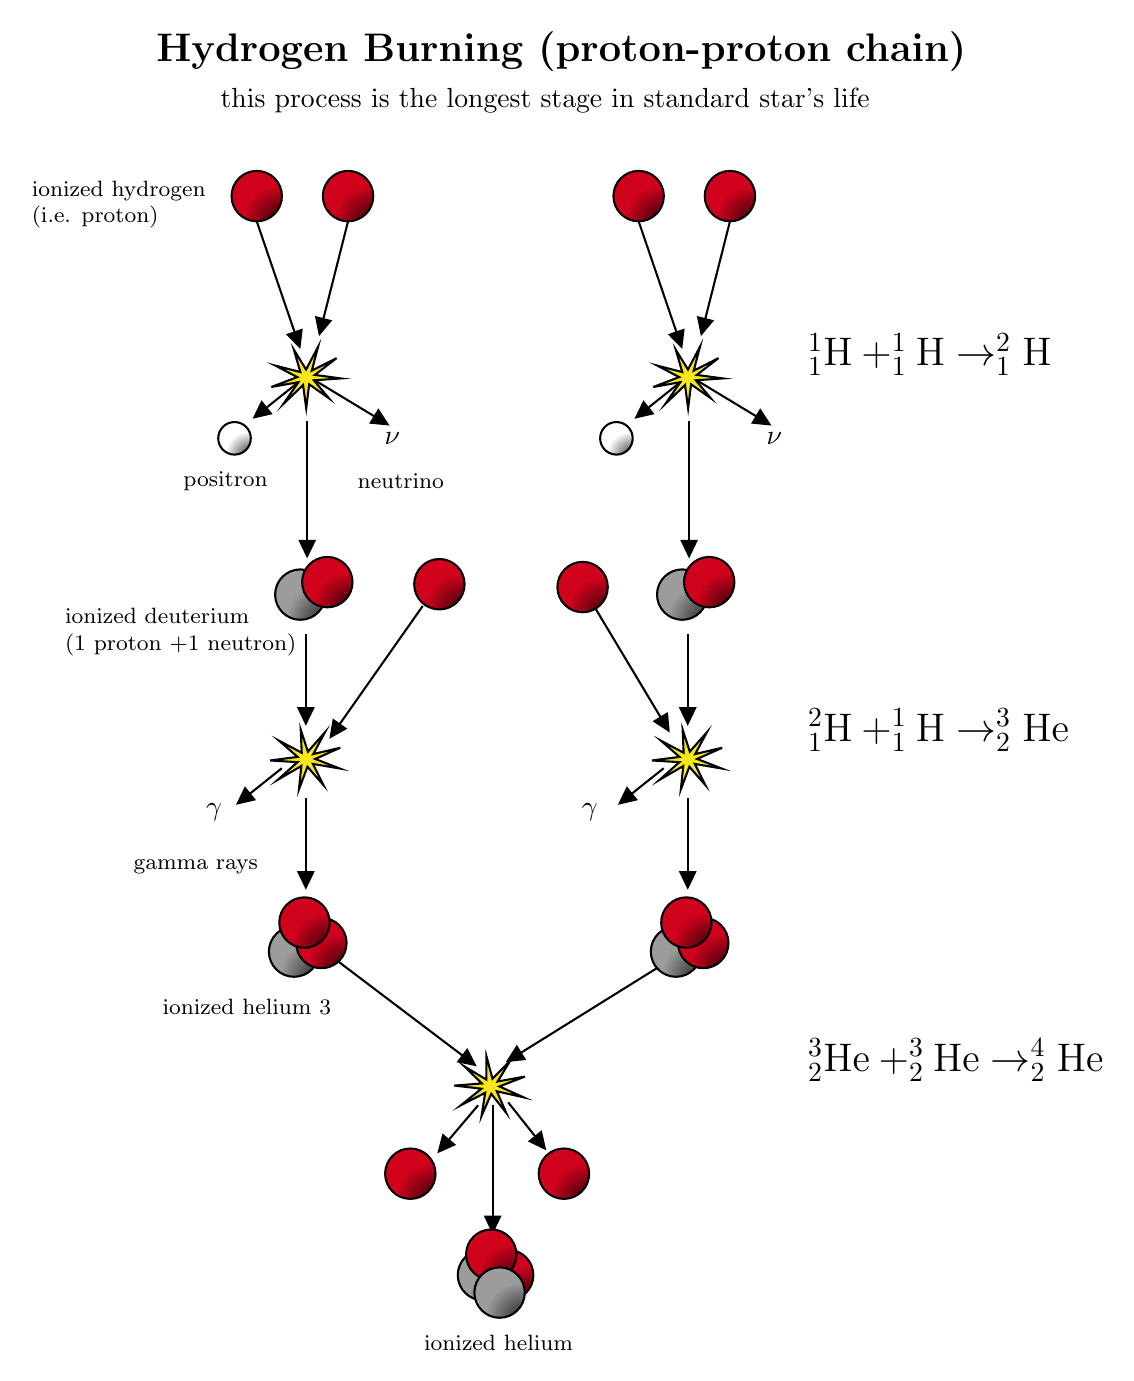
\begin{tikzpicture}[x=0.75pt,y=0.75pt,yscale=-1,xscale=1]
		%uncomment if require: \path (0,1222); %set diagram left start at 0, and has height of 1222
		
		%Shape: Circle [id:dp8962573722751259] 
		\path  [shading=_axrj1qrf1,_cblzk72s8] (173.72,303.64) .. controls (173.72,296.93) and (179.16,291.5) .. (185.86,291.5) .. controls (192.57,291.5) and (198,296.93) .. (198,303.64) .. controls (198,310.34) and (192.57,315.78) .. (185.86,315.78) .. controls (179.16,315.78) and (173.72,310.34) .. (173.72,303.64) -- cycle ; % for fading 
		 \draw  [color={rgb, 255:red, 0; green, 0; blue, 0 }  ,draw opacity=1 ] (173.72,303.64) .. controls (173.72,296.93) and (179.16,291.5) .. (185.86,291.5) .. controls (192.57,291.5) and (198,296.93) .. (198,303.64) .. controls (198,310.34) and (192.57,315.78) .. (185.86,315.78) .. controls (179.16,315.78) and (173.72,310.34) .. (173.72,303.64) -- cycle ; % for border 
		
		%Shape: Circle [id:dp5725777248680912] 
		\path  [shading=_85hxa7f1s,_jvz4fq06k] (152.72,111.64) .. controls (152.72,104.93) and (158.16,99.5) .. (164.86,99.5) .. controls (171.57,99.5) and (177,104.93) .. (177,111.64) .. controls (177,118.34) and (171.57,123.78) .. (164.86,123.78) .. controls (158.16,123.78) and (152.72,118.34) .. (152.72,111.64) -- cycle ; % for fading 
		 \draw  [color={rgb, 255:red, 0; green, 0; blue, 0 }  ,draw opacity=1 ] (152.72,111.64) .. controls (152.72,104.93) and (158.16,99.5) .. (164.86,99.5) .. controls (171.57,99.5) and (177,104.93) .. (177,111.64) .. controls (177,118.34) and (171.57,123.78) .. (164.86,123.78) .. controls (158.16,123.78) and (152.72,118.34) .. (152.72,111.64) -- cycle ; % for border 
		
		%Shape: Circle [id:dp30921099949240194] 
		\path  [shading=_qgjp323p0,_a4qlb2nh4] (196.72,111.64) .. controls (196.72,104.93) and (202.16,99.5) .. (208.86,99.5) .. controls (215.57,99.5) and (221,104.93) .. (221,111.64) .. controls (221,118.34) and (215.57,123.78) .. (208.86,123.78) .. controls (202.16,123.78) and (196.72,118.34) .. (196.72,111.64) -- cycle ; % for fading 
		 \draw  [color={rgb, 255:red, 0; green, 0; blue, 0 }  ,draw opacity=1 ] (196.72,111.64) .. controls (196.72,104.93) and (202.16,99.5) .. (208.86,99.5) .. controls (215.57,99.5) and (221,104.93) .. (221,111.64) .. controls (221,118.34) and (215.57,123.78) .. (208.86,123.78) .. controls (202.16,123.78) and (196.72,118.34) .. (196.72,111.64) -- cycle ; % for border 
		
		%Straight Lines [id:da682986046600607] 
		\draw    (164.86,123.78) -- (184.89,182.44) ;
		\draw [shift={(185.86,185.28)}, rotate = 251.14] [fill={rgb, 255:red, 0; green, 0; blue, 0 }  ][line width=0.08]  [draw opacity=0] (8.93,-4.29) -- (0,0) -- (8.93,4.29) -- cycle    ;
		%Straight Lines [id:da36044520058108076] 
		\draw    (208.86,123.78) -- (195.6,176.19) ;
		\draw [shift={(194.86,179.1)}, rotate = 284.2] [fill={rgb, 255:red, 0; green, 0; blue, 0 }  ][line width=0.08]  [draw opacity=0] (8.93,-4.29) -- (0,0) -- (8.93,4.29) -- cycle    ;
		%Shape: Star [id:dp8812859524008496] 
		\draw  [fill={rgb, 255:red, 248; green, 231; blue, 28 }  ,fill opacity=1 ] (182.78,185.71) -- (188.63,195.2) -- (194.4,184.28) -- (191.4,195.74) -- (203.32,189.72) -- (192.88,197.79) -- (205.38,199.49) -- (192.38,200.39) -- (199.61,209.02) -- (190.13,202.33) -- (188.7,213.84) -- (187.19,202.69) -- (177.77,211.71) -- (184.92,201.31) -- (171.92,203.61) -- (184.4,198.84) -- (173.9,193.34) -- (185.87,196.42) -- cycle ;
		%Straight Lines [id:da8746124137214746] 
		\draw    (192.84,200.39) -- (226.3,220.63) ;
		\draw [shift={(228.86,222.19)}, rotate = 211.17] [fill={rgb, 255:red, 0; green, 0; blue, 0 }  ][line width=0.08]  [draw opacity=0] (8.93,-4.29) -- (0,0) -- (8.93,4.29) -- cycle    ;
		%Shape: Circle [id:dp1809819460318527] 
		\path  [shading=_gyz9dzgv9,_pum4h8add] (146.31,228.34) .. controls (146.31,224.01) and (149.82,220.5) .. (154.16,220.5) .. controls (158.49,220.5) and (162,224.01) .. (162,228.34) .. controls (162,232.68) and (158.49,236.19) .. (154.16,236.19) .. controls (149.82,236.19) and (146.31,232.68) .. (146.31,228.34) -- cycle ; % for fading 
		 \draw  [color={rgb, 255:red, 0; green, 0; blue, 0 }  ,draw opacity=1 ] (146.31,228.34) .. controls (146.31,224.01) and (149.82,220.5) .. (154.16,220.5) .. controls (158.49,220.5) and (162,224.01) .. (162,228.34) .. controls (162,232.68) and (158.49,236.19) .. (154.16,236.19) .. controls (149.82,236.19) and (146.31,232.68) .. (146.31,228.34) -- cycle ; % for border 
		
		%Straight Lines [id:da0664471390597321] 
		\draw    (184.92,201.31) -- (165.21,217.04) ;
		\draw [shift={(162.86,218.91)}, rotate = 321.41] [fill={rgb, 255:red, 0; green, 0; blue, 0 }  ][line width=0.08]  [draw opacity=0] (8.93,-4.29) -- (0,0) -- (8.93,4.29) -- cycle    ;
		%Straight Lines [id:da21138746811957376] 
		\draw    (189.17,220.19) -- (189.17,283.19) ;
		\draw [shift={(189.17,286.19)}, rotate = 270] [fill={rgb, 255:red, 0; green, 0; blue, 0 }  ][line width=0.08]  [draw opacity=0] (8.93,-4.29) -- (0,0) -- (8.93,4.29) -- cycle    ;
		%Shape: Circle [id:dp013176562497542843] 
		\path  [shading=_gs9v2qfgw,_0rrvhevqy] (186.72,297.64) .. controls (186.72,290.93) and (192.16,285.5) .. (198.86,285.5) .. controls (205.57,285.5) and (211,290.93) .. (211,297.64) .. controls (211,304.34) and (205.57,309.78) .. (198.86,309.78) .. controls (192.16,309.78) and (186.72,304.34) .. (186.72,297.64) -- cycle ; % for fading 
		 \draw  [color={rgb, 255:red, 0; green, 0; blue, 0 }  ,draw opacity=1 ] (186.72,297.64) .. controls (186.72,290.93) and (192.16,285.5) .. (198.86,285.5) .. controls (205.57,285.5) and (211,290.93) .. (211,297.64) .. controls (211,304.34) and (205.57,309.78) .. (198.86,309.78) .. controls (192.16,309.78) and (186.72,304.34) .. (186.72,297.64) -- cycle ; % for border 
		
		%Shape: Star [id:dp5749059916858088] 
		\draw  [fill={rgb, 255:red, 248; green, 231; blue, 28 }  ,fill opacity=1 ] (186.06,368.7) -- (189.51,379.3) -- (197.69,370.04) -- (192.08,380.48) -- (205.09,377.43) -- (193.04,382.82) -- (204.79,387.41) -- (191.94,385.23) -- (196.94,395.31) -- (189.3,386.58) -- (185.21,397.44) -- (186.35,386.24) -- (175.08,392.8) -- (184.48,384.37) -- (171.3,383.56) -- (184.55,381.84) -- (175.64,374.04) -- (186.54,379.84) -- cycle ;
		%Shape: Circle [id:dp5545180078282128] 
		\path  [shading=_my8z4jtth,_g725wvp4c] (240.72,298.64) .. controls (240.72,291.93) and (246.16,286.5) .. (252.86,286.5) .. controls (259.57,286.5) and (265,291.93) .. (265,298.64) .. controls (265,305.34) and (259.57,310.78) .. (252.86,310.78) .. controls (246.16,310.78) and (240.72,305.34) .. (240.72,298.64) -- cycle ; % for fading 
		 \draw  [color={rgb, 255:red, 0; green, 0; blue, 0 }  ,draw opacity=1 ] (240.72,298.64) .. controls (240.72,291.93) and (246.16,286.5) .. (252.86,286.5) .. controls (259.57,286.5) and (265,291.93) .. (265,298.64) .. controls (265,305.34) and (259.57,310.78) .. (252.86,310.78) .. controls (246.16,310.78) and (240.72,305.34) .. (240.72,298.64) -- cycle ; % for border 
		
		%Straight Lines [id:da8740249941190632] 
		\draw    (188.52,322.7) -- (188.52,363.84) ;
		\draw [shift={(188.52,366.84)}, rotate = 270] [fill={rgb, 255:red, 0; green, 0; blue, 0 }  ][line width=0.08]  [draw opacity=0] (8.93,-4.29) -- (0,0) -- (8.93,4.29) -- cycle    ;
		%Straight Lines [id:da023367958589334714] 
		\draw    (244.86,309.1) -- (201.59,370.64) ;
		\draw [shift={(199.86,373.1)}, rotate = 305.11] [fill={rgb, 255:red, 0; green, 0; blue, 0 }  ][line width=0.08]  [draw opacity=0] (8.93,-4.29) -- (0,0) -- (8.93,4.29) -- cycle    ;
		%Straight Lines [id:da5192113183434639] 
		\draw    (188.52,401.7) -- (188.52,442.84) ;
		\draw [shift={(188.52,445.84)}, rotate = 270] [fill={rgb, 255:red, 0; green, 0; blue, 0 }  ][line width=0.08]  [draw opacity=0] (8.93,-4.29) -- (0,0) -- (8.93,4.29) -- cycle    ;
		%Straight Lines [id:da3577142574160339] 
		\draw    (176.92,387.31) -- (157.21,403.04) ;
		\draw [shift={(154.86,404.91)}, rotate = 321.41] [fill={rgb, 255:red, 0; green, 0; blue, 0 }  ][line width=0.08]  [draw opacity=0] (8.93,-4.29) -- (0,0) -- (8.93,4.29) -- cycle    ;
		%Shape: Circle [id:dp6775244978424118] 
		\path  [shading=_ygoewra8d,_f1mnrxgwm] (170.72,475.64) .. controls (170.72,468.93) and (176.16,463.5) .. (182.86,463.5) .. controls (189.57,463.5) and (195,468.93) .. (195,475.64) .. controls (195,482.34) and (189.57,487.78) .. (182.86,487.78) .. controls (176.16,487.78) and (170.72,482.34) .. (170.72,475.64) -- cycle ; % for fading 
		 \draw  [color={rgb, 255:red, 0; green, 0; blue, 0 }  ,draw opacity=1 ] (170.72,475.64) .. controls (170.72,468.93) and (176.16,463.5) .. (182.86,463.5) .. controls (189.57,463.5) and (195,468.93) .. (195,475.64) .. controls (195,482.34) and (189.57,487.78) .. (182.86,487.78) .. controls (176.16,487.78) and (170.72,482.34) .. (170.72,475.64) -- cycle ; % for border 
		
		%Shape: Circle [id:dp8834179578629084] 
		\path  [shading=_9hntko4f2,_akn9nqmzu] (183.86,471.5) .. controls (183.86,464.8) and (189.3,459.36) .. (196,459.36) .. controls (202.7,459.36) and (208.14,464.8) .. (208.14,471.5) .. controls (208.14,478.2) and (202.7,483.64) .. (196,483.64) .. controls (189.3,483.64) and (183.86,478.2) .. (183.86,471.5) -- cycle ; % for fading 
		 \draw  [color={rgb, 255:red, 0; green, 0; blue, 0 }  ,draw opacity=1 ] (183.86,471.5) .. controls (183.86,464.8) and (189.3,459.36) .. (196,459.36) .. controls (202.7,459.36) and (208.14,464.8) .. (208.14,471.5) .. controls (208.14,478.2) and (202.7,483.64) .. (196,483.64) .. controls (189.3,483.64) and (183.86,478.2) .. (183.86,471.5) -- cycle ; % for border 
		
		%Shape: Circle [id:dp4011096696346006] 
		\path  [shading=_rk80eilmp,_iz64l60of] (175.72,461.64) .. controls (175.72,454.93) and (181.16,449.5) .. (187.86,449.5) .. controls (194.57,449.5) and (200,454.93) .. (200,461.64) .. controls (200,468.34) and (194.57,473.78) .. (187.86,473.78) .. controls (181.16,473.78) and (175.72,468.34) .. (175.72,461.64) -- cycle ; % for fading 
		 \draw  [color={rgb, 255:red, 0; green, 0; blue, 0 }  ,draw opacity=1 ] (175.72,461.64) .. controls (175.72,454.93) and (181.16,449.5) .. (187.86,449.5) .. controls (194.57,449.5) and (200,454.93) .. (200,461.64) .. controls (200,468.34) and (194.57,473.78) .. (187.86,473.78) .. controls (181.16,473.78) and (175.72,468.34) .. (175.72,461.64) -- cycle ; % for border 
		
		%Shape: Circle [id:dp07066797634211652] 
		\path  [shading=_c51t3e7vf,_x85b74kc2] (357.72,303.64) .. controls (357.72,296.93) and (363.16,291.5) .. (369.86,291.5) .. controls (376.57,291.5) and (382,296.93) .. (382,303.64) .. controls (382,310.34) and (376.57,315.78) .. (369.86,315.78) .. controls (363.16,315.78) and (357.72,310.34) .. (357.72,303.64) -- cycle ; % for fading 
		 \draw  [color={rgb, 255:red, 0; green, 0; blue, 0 }  ,draw opacity=1 ] (357.72,303.64) .. controls (357.72,296.93) and (363.16,291.5) .. (369.86,291.5) .. controls (376.57,291.5) and (382,296.93) .. (382,303.64) .. controls (382,310.34) and (376.57,315.78) .. (369.86,315.78) .. controls (363.16,315.78) and (357.72,310.34) .. (357.72,303.64) -- cycle ; % for border 
		
		%Shape: Circle [id:dp55110431998894] 
		\path  [shading=_iztba8ahv,_ssnvdjv48] (336.72,111.64) .. controls (336.72,104.93) and (342.16,99.5) .. (348.86,99.5) .. controls (355.57,99.5) and (361,104.93) .. (361,111.64) .. controls (361,118.34) and (355.57,123.78) .. (348.86,123.78) .. controls (342.16,123.78) and (336.72,118.34) .. (336.72,111.64) -- cycle ; % for fading 
		 \draw  [color={rgb, 255:red, 0; green, 0; blue, 0 }  ,draw opacity=1 ] (336.72,111.64) .. controls (336.72,104.93) and (342.16,99.5) .. (348.86,99.5) .. controls (355.57,99.5) and (361,104.93) .. (361,111.64) .. controls (361,118.34) and (355.57,123.78) .. (348.86,123.78) .. controls (342.16,123.78) and (336.72,118.34) .. (336.72,111.64) -- cycle ; % for border 
		
		%Shape: Circle [id:dp558237084148518] 
		\path  [shading=_2pszfhkw3,_p6y8bsv8e] (380.72,111.64) .. controls (380.72,104.93) and (386.16,99.5) .. (392.86,99.5) .. controls (399.57,99.5) and (405,104.93) .. (405,111.64) .. controls (405,118.34) and (399.57,123.78) .. (392.86,123.78) .. controls (386.16,123.78) and (380.72,118.34) .. (380.72,111.64) -- cycle ; % for fading 
		 \draw  [color={rgb, 255:red, 0; green, 0; blue, 0 }  ,draw opacity=1 ] (380.72,111.64) .. controls (380.72,104.93) and (386.16,99.5) .. (392.86,99.5) .. controls (399.57,99.5) and (405,104.93) .. (405,111.64) .. controls (405,118.34) and (399.57,123.78) .. (392.86,123.78) .. controls (386.16,123.78) and (380.72,118.34) .. (380.72,111.64) -- cycle ; % for border 
		
		%Straight Lines [id:da810094213403945] 
		\draw    (348.86,123.78) -- (368.89,182.44) ;
		\draw [shift={(369.86,185.28)}, rotate = 251.14] [fill={rgb, 255:red, 0; green, 0; blue, 0 }  ][line width=0.08]  [draw opacity=0] (8.93,-4.29) -- (0,0) -- (8.93,4.29) -- cycle    ;
		%Straight Lines [id:da20922642388366075] 
		\draw    (392.86,123.78) -- (379.6,176.19) ;
		\draw [shift={(378.86,179.1)}, rotate = 284.2] [fill={rgb, 255:red, 0; green, 0; blue, 0 }  ][line width=0.08]  [draw opacity=0] (8.93,-4.29) -- (0,0) -- (8.93,4.29) -- cycle    ;
		%Shape: Star [id:dp6204774846453969] 
		\draw  [fill={rgb, 255:red, 248; green, 231; blue, 28 }  ,fill opacity=1 ] (366.78,185.71) -- (372.63,195.2) -- (378.4,184.28) -- (375.4,195.74) -- (387.32,189.72) -- (376.88,197.79) -- (389.38,199.49) -- (376.38,200.39) -- (383.61,209.02) -- (374.13,202.33) -- (372.7,213.84) -- (371.19,202.69) -- (361.77,211.71) -- (368.92,201.31) -- (355.92,203.61) -- (368.4,198.84) -- (357.9,193.34) -- (369.87,196.42) -- cycle ;
		%Straight Lines [id:da473704197496261] 
		\draw    (376.84,200.39) -- (410.3,220.63) ;
		\draw [shift={(412.86,222.19)}, rotate = 211.17] [fill={rgb, 255:red, 0; green, 0; blue, 0 }  ][line width=0.08]  [draw opacity=0] (8.93,-4.29) -- (0,0) -- (8.93,4.29) -- cycle    ;
		%Shape: Circle [id:dp4419694648671251] 
		\path  [shading=_wsxl0p4oe,_e5j4hqpz4] (330.31,228.34) .. controls (330.31,224.01) and (333.82,220.5) .. (338.16,220.5) .. controls (342.49,220.5) and (346,224.01) .. (346,228.34) .. controls (346,232.68) and (342.49,236.19) .. (338.16,236.19) .. controls (333.82,236.19) and (330.31,232.68) .. (330.31,228.34) -- cycle ; % for fading 
		 \draw  [color={rgb, 255:red, 0; green, 0; blue, 0 }  ,draw opacity=1 ] (330.31,228.34) .. controls (330.31,224.01) and (333.82,220.5) .. (338.16,220.5) .. controls (342.49,220.5) and (346,224.01) .. (346,228.34) .. controls (346,232.68) and (342.49,236.19) .. (338.16,236.19) .. controls (333.82,236.19) and (330.31,232.68) .. (330.31,228.34) -- cycle ; % for border 
		
		%Straight Lines [id:da6380295358642907] 
		\draw    (368.92,201.31) -- (349.21,217.04) ;
		\draw [shift={(346.86,218.91)}, rotate = 321.41] [fill={rgb, 255:red, 0; green, 0; blue, 0 }  ][line width=0.08]  [draw opacity=0] (8.93,-4.29) -- (0,0) -- (8.93,4.29) -- cycle    ;
		%Straight Lines [id:da29784090738060565] 
		\draw    (373.17,220.19) -- (373.17,283.19) ;
		\draw [shift={(373.17,286.19)}, rotate = 270] [fill={rgb, 255:red, 0; green, 0; blue, 0 }  ][line width=0.08]  [draw opacity=0] (8.93,-4.29) -- (0,0) -- (8.93,4.29) -- cycle    ;
		%Shape: Circle [id:dp6034018346442105] 
		\path  [shading=_44o8f4o87,_br5aheh7w] (370.72,297.64) .. controls (370.72,290.93) and (376.16,285.5) .. (382.86,285.5) .. controls (389.57,285.5) and (395,290.93) .. (395,297.64) .. controls (395,304.34) and (389.57,309.78) .. (382.86,309.78) .. controls (376.16,309.78) and (370.72,304.34) .. (370.72,297.64) -- cycle ; % for fading 
		 \draw  [color={rgb, 255:red, 0; green, 0; blue, 0 }  ,draw opacity=1 ] (370.72,297.64) .. controls (370.72,290.93) and (376.16,285.5) .. (382.86,285.5) .. controls (389.57,285.5) and (395,290.93) .. (395,297.64) .. controls (395,304.34) and (389.57,309.78) .. (382.86,309.78) .. controls (376.16,309.78) and (370.72,304.34) .. (370.72,297.64) -- cycle ; % for border 
		
		%Shape: Star [id:dp8424942502353532] 
		\draw  [fill={rgb, 255:red, 248; green, 231; blue, 28 }  ,fill opacity=1 ] (370.06,368.7) -- (373.51,379.3) -- (381.69,370.04) -- (376.08,380.48) -- (389.09,377.43) -- (377.04,382.82) -- (388.79,387.41) -- (375.94,385.23) -- (380.94,395.31) -- (373.3,386.58) -- (369.21,397.44) -- (370.35,386.24) -- (359.08,392.8) -- (368.48,384.37) -- (355.3,383.56) -- (368.55,381.84) -- (359.64,374.04) -- (370.54,379.84) -- cycle ;
		%Straight Lines [id:da786733166255011] 
		\draw    (372.52,322.7) -- (372.52,363.84) ;
		\draw [shift={(372.52,366.84)}, rotate = 270] [fill={rgb, 255:red, 0; green, 0; blue, 0 }  ][line width=0.08]  [draw opacity=0] (8.93,-4.29) -- (0,0) -- (8.93,4.29) -- cycle    ;
		%Straight Lines [id:da07224367747403715] 
		\draw    (321.86,300.01) -- (362.32,367.52) ;
		\draw [shift={(363.86,370.1)}, rotate = 239.07] [fill={rgb, 255:red, 0; green, 0; blue, 0 }  ][line width=0.08]  [draw opacity=0] (8.93,-4.29) -- (0,0) -- (8.93,4.29) -- cycle    ;
		%Straight Lines [id:da07573888100550308] 
		\draw    (372.52,401.7) -- (372.52,442.84) ;
		\draw [shift={(372.52,445.84)}, rotate = 270] [fill={rgb, 255:red, 0; green, 0; blue, 0 }  ][line width=0.08]  [draw opacity=0] (8.93,-4.29) -- (0,0) -- (8.93,4.29) -- cycle    ;
		%Straight Lines [id:da24121776077187929] 
		\draw    (360.92,387.31) -- (341.21,403.04) ;
		\draw [shift={(338.86,404.91)}, rotate = 321.41] [fill={rgb, 255:red, 0; green, 0; blue, 0 }  ][line width=0.08]  [draw opacity=0] (8.93,-4.29) -- (0,0) -- (8.93,4.29) -- cycle    ;
		%Shape: Circle [id:dp2135599963515098] 
		\path  [shading=_e9cun5z2f,_rbmv2gvjg] (354.72,475.64) .. controls (354.72,468.93) and (360.16,463.5) .. (366.86,463.5) .. controls (373.57,463.5) and (379,468.93) .. (379,475.64) .. controls (379,482.34) and (373.57,487.78) .. (366.86,487.78) .. controls (360.16,487.78) and (354.72,482.34) .. (354.72,475.64) -- cycle ; % for fading 
		 \draw  [color={rgb, 255:red, 0; green, 0; blue, 0 }  ,draw opacity=1 ] (354.72,475.64) .. controls (354.72,468.93) and (360.16,463.5) .. (366.86,463.5) .. controls (373.57,463.5) and (379,468.93) .. (379,475.64) .. controls (379,482.34) and (373.57,487.78) .. (366.86,487.78) .. controls (360.16,487.78) and (354.72,482.34) .. (354.72,475.64) -- cycle ; % for border 
		
		%Shape: Circle [id:dp23624279679235083] 
		\path  [shading=_eejk8j6cf,_tyoym1my4] (367.86,471.5) .. controls (367.86,464.8) and (373.3,459.36) .. (380,459.36) .. controls (386.7,459.36) and (392.14,464.8) .. (392.14,471.5) .. controls (392.14,478.2) and (386.7,483.64) .. (380,483.64) .. controls (373.3,483.64) and (367.86,478.2) .. (367.86,471.5) -- cycle ; % for fading 
		 \draw  [color={rgb, 255:red, 0; green, 0; blue, 0 }  ,draw opacity=1 ] (367.86,471.5) .. controls (367.86,464.8) and (373.3,459.36) .. (380,459.36) .. controls (386.7,459.36) and (392.14,464.8) .. (392.14,471.5) .. controls (392.14,478.2) and (386.7,483.64) .. (380,483.64) .. controls (373.3,483.64) and (367.86,478.2) .. (367.86,471.5) -- cycle ; % for border 
		
		%Shape: Circle [id:dp6338208506706906] 
		\path  [shading=_yxbdgavie,_ieevsdram] (359.72,461.64) .. controls (359.72,454.93) and (365.16,449.5) .. (371.86,449.5) .. controls (378.57,449.5) and (384,454.93) .. (384,461.64) .. controls (384,468.34) and (378.57,473.78) .. (371.86,473.78) .. controls (365.16,473.78) and (359.72,468.34) .. (359.72,461.64) -- cycle ; % for fading 
		 \draw  [color={rgb, 255:red, 0; green, 0; blue, 0 }  ,draw opacity=1 ] (359.72,461.64) .. controls (359.72,454.93) and (365.16,449.5) .. (371.86,449.5) .. controls (378.57,449.5) and (384,454.93) .. (384,461.64) .. controls (384,468.34) and (378.57,473.78) .. (371.86,473.78) .. controls (365.16,473.78) and (359.72,468.34) .. (359.72,461.64) -- cycle ; % for border 
		
		%Shape: Circle [id:dp24642449000513134] 
		\path  [shading=_dkwe5k4rm,_mlbxzhx0n] (309.72,300.01) .. controls (309.72,293.3) and (315.16,287.87) .. (321.86,287.87) .. controls (328.57,287.87) and (334,293.3) .. (334,300.01) .. controls (334,306.71) and (328.57,312.14) .. (321.86,312.14) .. controls (315.16,312.14) and (309.72,306.71) .. (309.72,300.01) -- cycle ; % for fading 
		 \draw  [color={rgb, 255:red, 0; green, 0; blue, 0 }  ,draw opacity=1 ] (309.72,300.01) .. controls (309.72,293.3) and (315.16,287.87) .. (321.86,287.87) .. controls (328.57,287.87) and (334,293.3) .. (334,300.01) .. controls (334,306.71) and (328.57,312.14) .. (321.86,312.14) .. controls (315.16,312.14) and (309.72,306.71) .. (309.72,300.01) -- cycle ; % for border 
		
		%Straight Lines [id:da7882118934838731] 
		\draw    (204.52,480.7) -- (268.47,529.1) ;
		\draw [shift={(270.86,530.91)}, rotate = 217.12] [fill={rgb, 255:red, 0; green, 0; blue, 0 }  ][line width=0.08]  [draw opacity=0] (8.93,-4.29) -- (0,0) -- (8.93,4.29) -- cycle    ;
		%Straight Lines [id:da5184405757415529] 
		\draw    (357.52,483.7) -- (287.41,527.33) ;
		\draw [shift={(284.86,528.91)}, rotate = 328.11] [fill={rgb, 255:red, 0; green, 0; blue, 0 }  ][line width=0.08]  [draw opacity=0] (8.93,-4.29) -- (0,0) -- (8.93,4.29) -- cycle    ;
		%Shape: Star [id:dp5264396083454435] 
		\draw  [fill={rgb, 255:red, 248; green, 231; blue, 28 }  ,fill opacity=1 ] (275.55,526.13) -- (278.44,536.9) -- (287.09,528.08) -- (280.94,538.21) -- (294.09,535.85) -- (281.78,540.6) -- (293.27,545.8) -- (280.55,542.95) -- (285.02,553.28) -- (277.85,544.16) -- (273.19,554.79) -- (274.92,543.67) -- (263.32,549.62) -- (273.15,541.7) -- (260.03,540.19) -- (273.36,539.18) -- (264.86,530.91) -- (275.45,537.28) -- cycle ;
		%Straight Lines [id:da9505990743599804] 
		\draw    (278.52,549.7) -- (278.52,608.82) ;
		\draw [shift={(278.52,611.82)}, rotate = 270] [fill={rgb, 255:red, 0; green, 0; blue, 0 }  ][line width=0.08]  [draw opacity=0] (8.93,-4.29) -- (0,0) -- (8.93,4.29) -- cycle    ;
		%Straight Lines [id:da9106553873939758] 
		\draw    (271.52,549.7) -- (253.81,570.54) ;
		\draw [shift={(251.86,572.82)}, rotate = 310.37] [fill={rgb, 255:red, 0; green, 0; blue, 0 }  ][line width=0.08]  [draw opacity=0] (8.93,-4.29) -- (0,0) -- (8.93,4.29) -- cycle    ;
		%Straight Lines [id:da5522526752822454] 
		\draw    (286.02,548.28) -- (302.5,569.05) ;
		\draw [shift={(304.36,571.4)}, rotate = 231.58] [fill={rgb, 255:red, 0; green, 0; blue, 0 }  ][line width=0.08]  [draw opacity=0] (8.93,-4.29) -- (0,0) -- (8.93,4.29) -- cycle    ;
		%Shape: Circle [id:dp36939909264945237] 
		\path  [shading=_qz8vwzlfv,_67gxx937d] (226.72,582.64) .. controls (226.72,575.93) and (232.16,570.5) .. (238.86,570.5) .. controls (245.57,570.5) and (251,575.93) .. (251,582.64) .. controls (251,589.34) and (245.57,594.78) .. (238.86,594.78) .. controls (232.16,594.78) and (226.72,589.34) .. (226.72,582.64) -- cycle ; % for fading 
		 \draw  [color={rgb, 255:red, 0; green, 0; blue, 0 }  ,draw opacity=1 ] (226.72,582.64) .. controls (226.72,575.93) and (232.16,570.5) .. (238.86,570.5) .. controls (245.57,570.5) and (251,575.93) .. (251,582.64) .. controls (251,589.34) and (245.57,594.78) .. (238.86,594.78) .. controls (232.16,594.78) and (226.72,589.34) .. (226.72,582.64) -- cycle ; % for border 
		
		%Shape: Circle [id:dp19436171672107494] 
		\path  [shading=_xqb6k1gbk,_ozsnb6asp] (300.72,582.64) .. controls (300.72,575.93) and (306.16,570.5) .. (312.86,570.5) .. controls (319.57,570.5) and (325,575.93) .. (325,582.64) .. controls (325,589.34) and (319.57,594.78) .. (312.86,594.78) .. controls (306.16,594.78) and (300.72,589.34) .. (300.72,582.64) -- cycle ; % for fading 
		 \draw  [color={rgb, 255:red, 0; green, 0; blue, 0 }  ,draw opacity=1 ] (300.72,582.64) .. controls (300.72,575.93) and (306.16,570.5) .. (312.86,570.5) .. controls (319.57,570.5) and (325,575.93) .. (325,582.64) .. controls (325,589.34) and (319.57,594.78) .. (312.86,594.78) .. controls (306.16,594.78) and (300.72,589.34) .. (300.72,582.64) -- cycle ; % for border 
		
		%Shape: Circle [id:dp3763719433309485] 
		\path  [shading=_no3v3b8oj,_6rn7ody3o] (261.72,631.5) .. controls (261.72,624.8) and (267.16,619.36) .. (273.86,619.36) .. controls (280.57,619.36) and (286,624.8) .. (286,631.5) .. controls (286,638.2) and (280.57,643.64) .. (273.86,643.64) .. controls (267.16,643.64) and (261.72,638.2) .. (261.72,631.5) -- cycle ; % for fading 
		 \draw  [color={rgb, 255:red, 0; green, 0; blue, 0 }  ,draw opacity=1 ] (261.72,631.5) .. controls (261.72,624.8) and (267.16,619.36) .. (273.86,619.36) .. controls (280.57,619.36) and (286,624.8) .. (286,631.5) .. controls (286,638.2) and (280.57,643.64) .. (273.86,643.64) .. controls (267.16,643.64) and (261.72,638.2) .. (261.72,631.5) -- cycle ; % for border 
		
		%Shape: Circle [id:dp042068466428559104] 
		\path  [shading=_o0lqix1hl,_n17fffjlj] (273.86,631.5) .. controls (273.86,624.8) and (279.3,619.36) .. (286,619.36) .. controls (292.7,619.36) and (298.14,624.8) .. (298.14,631.5) .. controls (298.14,638.2) and (292.7,643.64) .. (286,643.64) .. controls (279.3,643.64) and (273.86,638.2) .. (273.86,631.5) -- cycle ; % for fading 
		 \draw  [color={rgb, 255:red, 0; green, 0; blue, 0 }  ,draw opacity=1 ] (273.86,631.5) .. controls (273.86,624.8) and (279.3,619.36) .. (286,619.36) .. controls (292.7,619.36) and (298.14,624.8) .. (298.14,631.5) .. controls (298.14,638.2) and (292.7,643.64) .. (286,643.64) .. controls (279.3,643.64) and (273.86,638.2) .. (273.86,631.5) -- cycle ; % for border 
		
		%Shape: Circle [id:dp44437266670737774] 
		\path  [shading=_tadrg9fi3,_9rqxdlct7] (265.72,621.64) .. controls (265.72,614.93) and (271.16,609.5) .. (277.86,609.5) .. controls (284.57,609.5) and (290,614.93) .. (290,621.64) .. controls (290,628.34) and (284.57,633.78) .. (277.86,633.78) .. controls (271.16,633.78) and (265.72,628.34) .. (265.72,621.64) -- cycle ; % for fading 
		 \draw  [color={rgb, 255:red, 0; green, 0; blue, 0 }  ,draw opacity=1 ] (265.72,621.64) .. controls (265.72,614.93) and (271.16,609.5) .. (277.86,609.5) .. controls (284.57,609.5) and (290,614.93) .. (290,621.64) .. controls (290,628.34) and (284.57,633.78) .. (277.86,633.78) .. controls (271.16,633.78) and (265.72,628.34) .. (265.72,621.64) -- cycle ; % for border 
		
		%Shape: Circle [id:dp02120688548246985] 
		\path  [shading=_g7ws58w0e,_fisp1p81i] (269.72,639.92) .. controls (269.72,633.21) and (275.16,627.78) .. (281.86,627.78) .. controls (288.57,627.78) and (294,633.21) .. (294,639.92) .. controls (294,646.62) and (288.57,652.06) .. (281.86,652.06) .. controls (275.16,652.06) and (269.72,646.62) .. (269.72,639.92) -- cycle ; % for fading 
		 \draw  [color={rgb, 255:red, 0; green, 0; blue, 0 }  ,draw opacity=1 ] (269.72,639.92) .. controls (269.72,633.21) and (275.16,627.78) .. (281.86,627.78) .. controls (288.57,627.78) and (294,633.21) .. (294,639.92) .. controls (294,646.62) and (288.57,652.06) .. (281.86,652.06) .. controls (275.16,652.06) and (269.72,646.62) .. (269.72,639.92) -- cycle ; % for border 
		
		
		% Text Node
		\draw (115,31) node [anchor=north west][inner sep=0.75pt]   [align=left] {\textbf{{\Large Hydrogen Burning (proton-proton chain)}}};
		% Text Node
		\draw (225,224.31) node [anchor=north west][inner sep=0.75pt]    {$\nu $};
		% Text Node
		\draw (429,176.31) node [anchor=north west][inner sep=0.75pt]  [font=\Large]  {$_{1}^{1}\mathrm{H} +_{1}^{1}\mathrm{H}\rightarrow _{1}^{2}\mathrm{H}$};
		% Text Node
		\draw (139,403.04) node [anchor=north west][inner sep=0.75pt]    {$\gamma $};
		% Text Node
		\draw (429,357.31) node [anchor=north west][inner sep=0.75pt]  [font=\Large]  {$_{1}^{2}\mathrm{H} +_{1}^{1}\mathrm{H}\rightarrow _{2}^{3}\mathrm{He}$};
		% Text Node
		\draw (409,224.31) node [anchor=north west][inner sep=0.75pt]    {$\nu $};
		% Text Node
		\draw (320,403.04) node [anchor=north west][inner sep=0.75pt]    {$\gamma $};
		% Text Node
		\draw (146,58) node [anchor=north west][inner sep=0.75pt]   [align=left] {this process is the longest stage in standard star's life};
		% Text Node
		\draw (429,516.31) node [anchor=north west][inner sep=0.75pt]  [font=\Large]  {$_{2}^{3}\mathrm{He} +_{2}^{3}\mathrm{He}\rightarrow _{2}^{4}\mathrm{He}$};
		% Text Node
		\draw (55,102.82) node [anchor=north west][inner sep=0.75pt]  [font=\footnotesize] [align=left] {ionized hydrogen\\(i.e. proton)};
		% Text Node
		\draw (128,242.82) node [anchor=north west][inner sep=0.75pt]  [font=\footnotesize] [align=left] {positron};
		% Text Node
		\draw (212,243.82) node [anchor=north west][inner sep=0.75pt]  [font=\footnotesize] [align=left] {neutrino};
		% Text Node
		\draw (71,308.82) node [anchor=north west][inner sep=0.75pt]  [font=\footnotesize] [align=left] {ionized deuterium\\(1 proton +1 neutron)};
		% Text Node
		\draw (104,429.82) node [anchor=north west][inner sep=0.75pt]  [font=\footnotesize] [align=left] {gamma rays};
		% Text Node
		\draw (118,496.82) node [anchor=north west][inner sep=0.75pt]  [font=\footnotesize] [align=left] {ionized helium 3};
		% Text Node
		\draw (244,658.82) node [anchor=north west][inner sep=0.75pt]  [font=\footnotesize] [align=left] {ionized helium};
		\end{tikzpicture}
		\vspace*{3mm}
		\caption[Diagram of the proton-proton chain reaction in typical Sun size stars]{Diagram of the proton-proton chain reaction\index{proton-proton chain reaction} in typical Sun size stars}
	\end{figure}
	The measurement of the mass of the proton gives $m_p\cong 1.673\cdot 10^{-27}$ [kg], while the helium mass is   $m_{\text{He}}\cong 6.645\cdot 10^{-27}$ [kg], that is to say a loss in atomic mass (we neglect the mass of positrons which is $10,000$ times smaller than that of the neutrino):
	
	So a relative loss of mass by fusion (this is the part of the reactions that escapes from the Sun in the form of kinetic energy):
	
	We will prove further below that the Sun emits a power output of:
	
	Therefore its mass consumption per second is:
	
	i.e. its mass decreases by $4.4$ million tonnes per second...
	
	Now we know that this value corresponds to only $0.72\%$ of the mass put in reaction in a fusion. The total mass reacted  is then (rule of three):
	
	Thus, at every second $627$ million tons of hydrogen 1(ionized) fuse into helium 4 with a weight loss of $4.4$ million tonnes which is converted into energy.
	
	Assuming that only the center of the Sun fills the thermal conditions for the fusion ($\cong 10\%$ of its total mass), this brings us to determine the time of nuclear life of the Sun (or any other Star of the same type whose mass is known):
	
	Transforming this in years we have:
	
	As we know that Earth is almost $4.5$ billion years that gives us an indication that the Sun has very likely already made more than half of its lifespan.
	
	If we apply the same calculations to the next step of our Sun, we get once all Hydrogen consumed transformed into Helium (at a temperature of 10 millions degrees to counterbalance gravity as we will prove it further below) a few million years before the next step. Then almost all Helium will be transformed into Carbon (as the pressure and therefore temperature increase to almso 200 million degrees to counterbalance gravity) and this state last only a few hundred thousands years before the next step. Then almost all Carbon will be transformed into Neon and this state last only a few thousands years before the next step. Then almost all Neon will be transformed into Oxygen and this state last only a few years before the next step.  Then almost all Oxygen will be transformed into Silicon and this state last only a few months before the next step. Then almost all Silicon will be transformed into Nickel (at a temperature of 2.5 billion degrees) and this state last only a few weeks before the next step. As Nickel decays into Iron (one of the most stable elements) afterwards it can happen that the stars collapse into a neutron star, or even a quark star or in some cases in a Black Hole.
	
	\paragraph{Internal Temperature}\mbox{}\\\\\
	The stars are assumed to be spherical clusters of hydrogen gas where the interactions between molecules are governed by the gravitational attraction.

	A star has no wall that delimits it, that is to say that there are no external forces coming from vacuum and therefore:
	
	and also not any bulk modulus.
	\begin{figure}[H]
		\centering
		\includegraphics[scale=0.23]{img/cosmology/sun_corona.jpg}	
		\caption[Sun Corona zoom]{Sun Corona zoom (source: NASA Goddard Space Flight Center)}
	\end{figure}
	\begin{tcolorbox}[title=Remark,arc=10pt,breakable,drop lifted shadow,
  skin=enhanced,
  skin first is subskin of={enhancedfirst}{arc=10pt,no shadow},
  skin middle is subskin of={enhancedmiddle}{arc=10pt,no shadow},
  skin last is subskin of={enhancedlast}{drop lifted shadow}]
	A solar flare is an intense localized eruption of electromagnetic radiation in the Sun's atmosphere that occur in active regions and are often, but not always, accompanied by coronal mass ejections, solar particle events, and other solar phenomena. The occurrence of solar flares varies with the actual 11-year solar cycle. Solar flares are thought to occur when stored magnetic energy in the Sun's atmosphere accelerates charged particles in the surrounding plasma. This results in the emission of electromagnetic radiation across the electromagnetic spectrum. 
High-energy electromagnetic radiation from solar flares is absorbed by the daylight side of Earth's upper atmosphere, in particular the ionosphere, and does not reach the surface most of the time. This absorption can temporarily increase the ionization of the ionosphere which may interfere with short-wave radio communication. The prediction of solar flares is an active area of research. Solar flares occur in a power-law spectrum of magnitudes; an energy release of typically $10^{20}$ joules of energy suffices to produce a clearly observable event, while a major event can emit up to $10^{25}$ joules (estimated value of the Carrington event that has occurred in 11859 according to holocene calendar).\\

	The National Oceanic and Atmosopheric Administration ranks geomagnetic storms on a scale running from G1, causing an increase in auroral activity and minor fluctuations in power supplies, up to G5, which includes extreme cases like the Carrington event.  Even a G2 event is capable of causing damages, as when SpaceX lost 40 satellites in Feb 2022 when a G2 storm prevented them reaching their intended altitude. According to \cite{lingam2017risks} speculation and worst case scenario, extreme solar flares from our Sun to an upper limit of $10^{28}$ joules (with a frequency of 26 million years to occur) may even lead to mass extinction event mainly because of the subsequent ozone layer depletion.
	\begin{table}[H]
		\centering
		\resizebox{\textwidth}{!}{
		\begin{tabular}{|c|c|c|c|c|}
		\hline \rowcolor[gray]{0.75} \textbf{Scale} & \textbf{Description} & \textbf{Effect} & $\begin{array}{l}\textbf { Physical } \\
		\textbf { measure }\end{array}$ & $\begin{array}{l}\textbf { Average Frequency } \\
		\text { (1 cycle }=11 \text { years) }\end{array}$ \\
		\hline \cellcolor[HTML]{CB0000}\textbf{G 5} & \textbf{Extreme} & $\begin{array}{l}\text { \textbf{Power systems:} Widespread voltage control problems and protective system problems can occur, some grid } \\
		\text { systems may experience complete collapse or blackouts. Transformers may experience damage. } \\
		\text { \textbf{Spacecraft operations:} May experience extensive surface charging, problems with orientation, uplink/downlink } \\
		\text { and tracking satellites. } \\
		\text { \textbf{Other systems:} Pipeline currents can reach hundreds of amps, HF (high frequency) radio propagation may be } \\
		\text { impossible in many areas for one to two days, satellite navigation may be degraded for days, low-frequency } \\
		\text { radio navigation can be out for hours, and aurora has been seen as low as Florida and southern Texas (typically } \\
		40^{\circ} \text { geomagnetic lat.). }\end{array}$ & $K p=9$ & $\begin{array}{l}4 \text { per cycle } \\
		\text { ( } 4 \text { days per cycle) }\end{array}$ \\
		\hline \cellcolor[HTML]{FE0000}\textbf{G 4} & \textbf{Severe} & $\begin{array}{l}\text { \textbf{Power systems:} Possible widespread voltage control problems and some protective systems will mistakenly trip } \\
		\text { out key assets from the grid. } \\
		\text { \textbf{Spacecraft operations:} May experience surface charging and tracking problems, corrections may be needed } \\
		\text { for orientation problems. } \\
		\text { \textbf{Other systems:} Induced pipeline currents affect preventive measures, HF radio propagation sporadic, satellite } \\
		\text { navigation degraded for hours, low-frequency radio navigation disrupted, and aurora has been seen as low as } \\
		\text { Alabama and northern California (typically } 45^{\circ} \text { geomagnetic lat.). }\end{array}$ & $\begin{array}{l}\mathrm{Kp}=8, \\
		\text { including a } \\
		9 \text { - }\end{array}$ & $\begin{array}{l}100 \text { per cycle } \\
		\text { (60 days per cycle) }\end{array}$ \\
		\hline \cellcolor[HTML]{F8A102} \textbf{G 3} & \textbf{Strong} & $\begin{array}{l}\text { \textbf{Power systems:} Voltage corrections may be required, false alarms triggered on some protection devices. } \\
		\text { \textbf{Spacecraft operations:} Surface charging may occur on satellite components, drag may increase on low-Earth- } \\
		\text { orbit satellites, and corrections may be needed for orientation problems. } \\
		\text {\textbf{ Other systems:} Intermittent satellite navigation and low-frequency radio navigation problems may occur, HF } \\
		\text { radio may be intermittent, and aurora has been seen as low as Illinois and Oregon (typically } 50^{\circ} \text { geomagnetic } \\
		\text { lat.). }\end{array}$ & $K p=7$ & $\begin{array}{l}200 \text { per cycle } \\
		\text { (130 days per cycle) }\end{array}$ \\
		\hline \cellcolor[HTML]{FFCC67}\textbf{G 2} & \textbf{Moderate} & $\begin{array}{l}\text { \textbf{Power systems:} High-latitude power systems may experience voltage alarms, long-duration storms may cause } \\
		\text { transformer damage. } \\
		\text { \textbf{Spacecraft operations:} Corrective actions to orientation may be required by ground control; possible changes } \\
		\text { in drag affect orbit predictions. } \\
		\text { \textbf{Other systems:} HF radio propagation can fade at higher latitudes, and aurora has been seen as low as New } \\
		\text { York and Idaho (typically } 55^{\circ} \text { geomagnetic lat.). }\end{array}$ & $K p=6$ & $\begin{array}{l}600 \text { per cycle } \\
		\text { (360 days per cycle) }\end{array}$ \\
		\hline \cellcolor[HTML]{FFFE65}\textbf{G 1} & \textbf{Minor} & $\begin{array}{l}\text { \textbf{Power systems:} Weak power grid fluctuations can occur. } \\
		\text { \textbf{Spacecraft operations:} Minor impact on satellite operations possible. } \\
		\text { \textbf{Other systems:} Migratory animals are affected at this and higher levels; aurora is commonly visible at high } \\
		\text { latitudes (northern Michigan and Maine). }\end{array}$ & $K p=5$ & $\begin{array}{l}1700 \text { per cycle } \\
		\text { (900 days per cycle) }\end{array}$ \\
		\hline
		\end{tabular}
		}
		\caption[Solar flares Geomagnetic scale]{Solar flares Geomagnetic scale (source: NOAA)}
	\end{table}
	Based on the return on experience of the G5 Carrington event and the Canada 11989 (holocene calendar) G5 event (the Miyake Event can't be used as 1400 years ago electric devices didn't exist), it's very unlikely that a even a super solar flare may damage HDD ans SSD drive. First because HDD drives already have magnets to make them work that are much stronger than G5 solar flares and SSD drive are said to be almost immune to magnetic fields. Instead, super solar flares can generate very high electrical currents in long conductors (i.e. long power grids), like power lines. These electrical surges can damage hardware connected to the grid just like a lightning strike. So if you have a Solar flare tracking app and get a G5 alarm, then just disconnect all your electric devices from the outlet (you don't need to put them in a Faraday cage or run into a nuclear basement, that's very likely useless). Some people say that SSD's are even immune to power outage.\\
	
	There is another common scale for solar flares:
	\begin{table}[H]
		\centering
		\begin{tabular}{|c|c|c|}
		\rowcolor[gray]{0.75} 
		\hline \textbf{Class} & \textbf{Intensity} $\left[\mathrm{W} \cdot \mathrm{m}^{-22}\right]$ & \textbf{Luminosity} $\left(\mathrm{L}_{\odot}, 100 \text{ sec}\right)$ \\
		\hline $\mathrm{B}$ & $10^{-7}$ & $10^{-8}$ \\
		\hline $\mathrm{C}$ & $10^{-6}$ & $10^{-7}$ \\
		\hline $\mathrm{M}$ & $10^{-5}$ & $10^{-6}$ \\
		\hline $\mathrm{X}$ & $10^{-4}$ & $10^{-5}$ \\
		\hline
		\end{tabular}
		\caption{Solar flares intensity scale}
	\end{table}
	An X2 is twice an X1. The 11989 (holocene calendar) event in Canada was a X7.3. The Carrington event was estimated X45 to X50.
	\end{tcolorbox}
	\begin{figure}[H]
		\centering
		\includegraphics[scale=0.75]{img/cosmology/global_sun.jpg}	
		\caption[Global Sun overview]{Global Sun overview (source: NASA)}
	\end{figure}
	Using the virial theorem proven in the section of Continuum Mechanics (see page \pageref{virial theorem}) that gives us:
	
	we have for a homogeneous spherical gas of radius $R$ and mass $M$ composed of $N$ bodies, the following relations proved for the first one in the section of Continuum Mechanics  (see page \pageref{equipartition theorem of energy}) of the second in the section of Classical Mechanics (see page \pageref{gravitational potential energy of a material sphere}):
	
	Therefore:
	
	where for recall $k$ is the Boltzmann constant.

	Which gives:
	
	in order to not make the confusion between to constant of ideal gas denoted $R$ and the radius it is more convenient to write the latter relation as (and making the Boltzmann constant more explicit):
	
	With for a given star $N$ being the ratio of the total mass of the star on the average mass of a molecule.
	
	For the Sun it comes that $T\cong 10^7$ [K] (i.e. $10$ millions degrees).
	
	This is the central temperature of the Sun. Optical measurements measured from Earth only give the surface temperature (chromosphere), thus $6,000$ [K]. The calculated internal temperature is about $1,600$ times higher than at the surface. Independent methods based on nuclear reactions in the center of the Sun (measurement of solar neutrino flux) give the same order of magnitude, but the precise values differ by a factor of $2$-$3$.
	
	\begin{table}[H]
		\centering
		\begin{tabular}{|l|l|l|}
		\hline
		\rowcolor[HTML]{C0C0C0} 
		\textbf{Layer} & \textbf{Part} & \textbf{Temperature {[}K{]}} \\ \hline
		 & Core & $15,000,000$ \\ \cline{2-3} 
		 & Radiative zone & $7,000,000$ \\ \cline{2-3} 
		\multirow{-3}{*}{Inner Layers} & Convection zone & $2,000,000$ \\ \hline
		 & Photosphere & $4,000$-$6,500$ \\ \cline{2-3} 
		 & Chromosphere & $4,000$-$8,000$ \\ \cline{2-3} 
		 & Transition region & $8,000$-$500,000$ \\ \cline{2-3} 
		\multirow{-4}{*}{Outer Layers} & Corona & $500,000$-$1,000,000$ \\ \hline
		\end{tabular}
		\caption{Summary of the average temperatures of typical Sun's layers}
	\end{table}
	Let us now see how good we can estimate the external temperature!
	
	\paragraph{External temperature}\mbox{}\\\\\
	We have proved in the section of Thermodynamics that the Stefan-Boltzmann law (see page \pageref{stefan boltzmann law}) permits to calculate the temperature of a heated body from its emittance or its internal energy in terms of density such as:
	
	with:
	
	where $\sigma_{\text{S.B.}}$ is Stefan-Boltzmann constant.

	Let us take an interesting example that concerns us directly:
	
	The average emittance also named "\NewTerm{average bolometric emittance}\index{average bolometric emittance}" received by the Earth outside the atmosphere, also named "\NewTerm{solar constant}\index{solar constant}" (which is in fact not constant ... on a scale of several billion years), is directly measurable in orbit and is equal to $\sim 1,373\;[\text{W}\cdot\text{m}^{-2}]$.
	
	Knowing the average distance from the Sun to be about $1.496\cdot 10^{11}\;[\text{m}]=1\;[\text{UA}]$  (Astronomical Unit), we can calculate the surface of the sphere at $R=1$ [UA] and thus the solar power $P$. Therefore:
	
	and:
	
	\begin{tcolorbox}[enhanced,title=Remark,colframe=black,arc=10pt,drop lifted shadow,after skip=15pt plus 2pt]
	From $P_{\odot}=S\cdot M(T)\cong 3.861\cdot 10^{26}\;[\text{W}]$ we can calculate the actual Solar flux (i.e. Sun flux) - or "peak Sun hours" - on Earth assuming that the latter is at an average distance of $149.09\cdot 10^{9}\;[\text{m}]$ of the Sun:
	$$\Phi=\dfrac{P_{\odot}}{4\pi R^2}=\dfrac{3.861\cdot 10^{26}}{4\pi (149.09\cdot 10^{9})^2}\cong 1,382 \;[\text{W}\cdot \text{m}^{-2}] $$
	Assuming an albedo for Earth of $\rho\cong 0.31$ (but there is considerable variation in this value over the surface of the Earth and over time as well), then:
	$$\Phi_\rho=(1-\rho)\cdot 1,382 \cong  953 \;[\text{W}\cdot \text{m}^{-2}] $$
	However the Earth isn't all the time facing the same part of its surface to the Sun. Assuming that only a third of a $24$ hours days is facing the Sun, then:
	$$\bar{\Phi}_\rho=\dfrac{1}{3}\cdot 1,382 \cong  318 \;[\text{W}\cdot \text{m}^{-2}] $$
	\end{tcolorbox}
	Assuming known the radius of the Sun as being $r_{\odot}\cong 6.9599\cdot 10^8$ [m], we can calculate its surface $S$ and its solar radiative emittance $M_{\odot}(T)$. So:
	
	and:
	
	\begin{tcolorbox}[title=Remark,arc=10pt,breakable,drop lifted shadow,
  skin=enhanced,
  skin first is subskin of={enhancedfirst}{arc=10pt,no shadow},
  skin middle is subskin of={enhancedmiddle}{arc=10pt,no shadow},
  skin last is subskin of={enhancedlast}{drop lifted shadow}]
	The radiating surface of a star is named "\NewTerm{photosphere}\index{photosphere}". Indeed, as stars, excepting neutron stars, have no solid surface, the photosphere is typically used to describe the Sun's or another star's visual surface.
	\end{tcolorbox}
	Using the Stefan-Boltzmann law (\SeeChapter{see section Statistical Mechanics page \pageref{stefan boltzmann law}}), we can now calculate approximately the thermodynamic temperature of the photosphere:
	
	which is very accurate to direct measurement!!! More generally the previous relation is written:
	
	or respecting the notation of optical geometry:
	
	So since we can estimate the luminosity and the temperature of a star (or something that looks like...) we can also estimate it's radius!
	\begin{figure}[H]
		\centering
		\includegraphics{img/cosmology/photosphere.jpg}	
		\caption[Layer's view of our Sun]{Layer's view of our Sun (source: NASA)}
	\end{figure}

	Planck's law (\SeeChapter{see section Thermodynamics page \pageref{planck law}}) applied at this temperature allow us to calculate the spectral distribution of solar radiation and then we see that the maximum of the intensity is in the visible range (our visible range!!!) spectrum which is from $400$ [nm] to $700$ [nm].
	
	Obviously the reader has to keep in mind that the temperature of a star is an  information that doesn't make really sense (we should speak instead of "average temperature", ie an integral of the spectrum function as we know it!) as the temperature depends on the wavelength. As provided by the paper \cite{cahalan2022solar}, we can see the temperature of our Sun in function of the wavelength here below as measured in the 12008-08-24 according to the holocene calendar (the lower figure is just a zoom on the visible spectrum):
	\begin{figure}[H]
		\centering
		\includegraphics[scale=0.8]{img/cosmology/sun_temperature_wavelength.jpg}	
		\caption[Sun temperature in function of wavelength]{Sun temperature in function of wavelength the 12008-08-24}
	\end{figure}
	And in the same paper we can see the evolution of our Sun's temperature for 17 years (daily average) on the $\mathrm{H}_\alpha$ wavelength ($656.2$ [nm]):
	\begin{figure}[H]
		\centering
		\includegraphics[scale=0.8]{img/cosmology/sun_temperature_years.jpg}	
		\caption{Sun temperature in function of time}
	\end{figure}
	In the above plot the years are given based on the Gregorian calendar.
	
	In the figure below, we can see an extrapolation of mean surface temperatures on Earth taking into account the slow increase of the insolation due to the aging of the Sun. Simulations where performed with a tridimensional global climate model described in Leconte et al. (2013; \url{https://ui.adsabs.harvard.edu/abs/2013Natur.504..268L/abstract}). When the average insolation received by the Earth reaches $375\; [\text{W}\cdot\text{m}^{-2}]$ (about 1 billion years from now), the greenhouse effect of water vapor enters a runaway regime that causes the total evaporation of the oceans. Temperatures above that threshold are very uncertain but could be greater than $1,000\;[^\circ \text{C}]$. 
	\begin{figure}[H]
		\centering
		\includegraphics[scale=0.6]{img/cosmology/earth_temperature_simulation.jpg}
		\vspace*{3mm}
		\caption[Computer simulation of Earth's temperature evolution]{Numerical simulations of the surface temperature of the Earth at the spring equinox\\ exposed to an increasingly bright Sun in the future.}
	\end{figure}
	So life will very likely disappear on Earth a veeeeery long time before the Sun turns into a supernova....
	
	\begin{tcolorbox}[title=Remark,arc=10pt,breakable,drop lifted shadow,
  skin=enhanced,
  skin first is subskin of={enhancedfirst}{arc=10pt,no shadow},
  skin middle is subskin of={enhancedmiddle}{arc=10pt,no shadow},
  skin last is subskin of={enhancedlast}{drop lifted shadow}]
	For information, the rotation of Earth's on itself slows down at the day we write these lines of approximately $2.3$ milliseconds per century. That means $1$ hour every $180$ millions years. Each year the Earth's orbit speed around the Sun also slows down of approximately $3$ nanometers-per-second. Using Kepler's law, that means that the Earth goes further away from the Sun of $3$ micrometers per $1$ billion year......!!!!
	\end{tcolorbox}
	
	\begin{figure}[H]
		\centering
		\includegraphics[width=0.9\textwidth]{img/cosmology/sun_layers_with_temperatures.jpg}	
		\caption[The layers of the Sun]{The layers of the Sun\\(source: \url{https://www.sciencefacts.net/layers-of-the-sun.html}, authors: Satyam Bhuyan, Santanu Mukherjee)}
	\end{figure}
	
	\paragraph{Equation of Hydrostatic Equilibrium}\mbox{}\\\\\
	The absence of changes in most stars over timescales of hours or days indicates that the forces acting on the matter in the stars are essentially perfectly balanced (remember figure showed earlier above). Here we analyse this constraint in more detail.

	In the figure below we have represented a piece mass shell in a spherically symmetric star where we consider in reality a very small cylindrical element between radius $r$ and radius $r + \mathrm{d}r$ hence the fact that the element surface $\mathrm{dS}$ is considered as being the same (but we can neglect the pressure variation as it can be very big even in a small height difference):
	\begin{figure}[H]
		\centering
		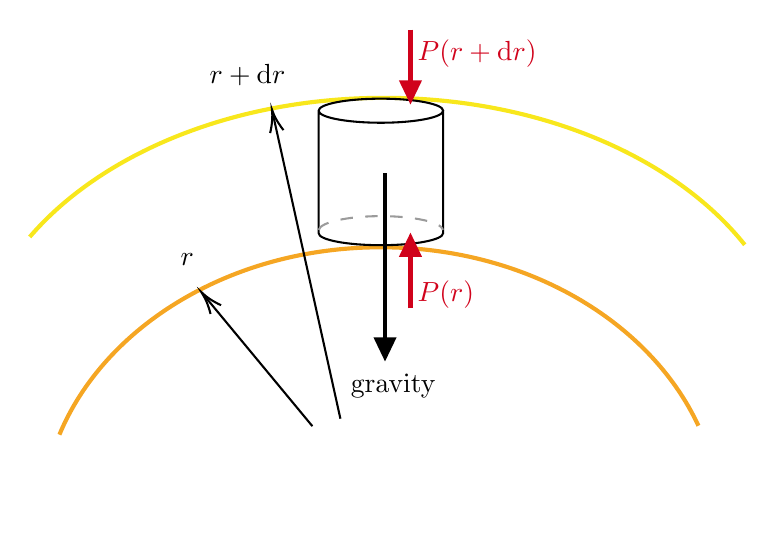
\begin{tikzpicture}[x=0.75pt,y=0.75pt,yscale=-1,xscale=1]
		%uncomment if require: \path (0,1046); %set diagram left start at 0, and has height of 1046
		
		%Shape: Arc [id:dp8236093165115685] 
		\draw  [draw opacity=0][line width=1.5]  (150.12,281.08) .. controls (171.99,228.58) and (233.07,190.8) .. (305,190.8) .. controls (374.95,190.8) and (434.65,226.54) .. (457.99,276.79) -- (305,323.8) -- cycle ; \draw  [color={rgb, 255:red, 245; green, 166; blue, 35 }  ,draw opacity=1 ][line width=1.5]  (150.12,281.08) .. controls (171.99,228.58) and (233.07,190.8) .. (305,190.8) .. controls (374.95,190.8) and (434.65,226.54) .. (457.99,276.79) ;  
		%Shape: Arc [id:dp6834541524542976] 
		\draw  [draw opacity=0][line width=1.5]  (135.83,185.81) .. controls (170.27,145.71) and (233.81,118.8) .. (306.5,118.8) .. controls (381.46,118.8) and (446.7,147.41) .. (480.31,189.61) -- (306.5,254.8) -- cycle ; \draw  [color={rgb, 255:red, 248; green, 231; blue, 28 }  ,draw opacity=1 ][line width=1.5]  (135.83,185.81) .. controls (170.27,145.71) and (233.81,118.8) .. (306.5,118.8) .. controls (381.46,118.8) and (446.7,147.41) .. (480.31,189.61) ;  
		%Straight Lines [id:da10692610380414536] 
		\draw    (272,277) -- (219.78,213.94) ;
		\draw [shift={(218.5,212.4)}, rotate = 50.37] [color={rgb, 255:red, 0; green, 0; blue, 0 }  ][line width=0.75]    (10.93,-3.29) .. controls (6.95,-1.4) and (3.31,-0.3) .. (0,0) .. controls (3.31,0.3) and (6.95,1.4) .. (10.93,3.29)   ;
		%Straight Lines [id:da3195723531521666] 
		\draw    (285.5,273.4) -- (252.93,126.35) ;
		\draw [shift={(252.5,124.4)}, rotate = 77.51] [color={rgb, 255:red, 0; green, 0; blue, 0 }  ][line width=0.75]    (10.93,-3.29) .. controls (6.95,-1.4) and (3.31,-0.3) .. (0,0) .. controls (3.31,0.3) and (6.95,1.4) .. (10.93,3.29)   ;
		%Shape: Can [id:dp2086822576132208] 
		\draw   (335,125) -- (335,184) .. controls (335,187.2) and (321.57,189.8) .. (305,189.8) .. controls (288.43,189.8) and (275,187.2) .. (275,184) -- (275,125) .. controls (275,121.8) and (288.43,119.2) .. (305,119.2) .. controls (321.57,119.2) and (335,121.8) .. (335,125) .. controls (335,128.2) and (321.57,130.8) .. (305,130.8) .. controls (288.43,130.8) and (275,128.2) .. (275,125) ;
		%Shape: Arc [id:dp2731992496837996] 
		\draw  [draw opacity=0][dash pattern={on 4.5pt off 4.5pt}] (275.04,182.42) .. controls (275.89,178.73) and (288.98,175.8) .. (305,175.8) .. controls (321,175.8) and (334.08,178.72) .. (334.95,182.41) -- (305,182.8) -- cycle ; \draw  [color={rgb, 255:red, 155; green, 155; blue, 155 }  ,draw opacity=1 ][dash pattern={on 4.5pt off 4.5pt}] (275.04,182.42) .. controls (275.89,178.73) and (288.98,175.8) .. (305,175.8) .. controls (321,175.8) and (334.08,178.72) .. (334.95,182.41) ;  
		%Straight Lines [id:da1507880981378642] 
		\draw [line width=1.5]    (307,155.2) -- (307,241.8) ;
		\draw [shift={(307,245.8)}, rotate = 270] [fill={rgb, 255:red, 0; green, 0; blue, 0 }  ][line width=0.08]  [draw opacity=0] (11.61,-5.58) -- (0,0) -- (11.61,5.58) -- cycle    ;
		%Straight Lines [id:da12665044389741587] 
		\draw [color={rgb, 255:red, 208; green, 2; blue, 27 }  ,draw opacity=1 ][line width=1.5]    (319.25,220.2) -- (319.25,187.8) ;
		\draw [shift={(319.25,183.8)}, rotate = 90] [fill={rgb, 255:red, 208; green, 2; blue, 27 }  ,fill opacity=1 ][line width=0.08]  [draw opacity=0] (11.61,-5.58) -- (0,0) -- (11.61,5.58) -- cycle    ;
		%Straight Lines [id:da04450833238333951] 
		\draw [color={rgb, 255:red, 208; green, 2; blue, 27 }  ,draw opacity=1 ][line width=1.5]    (319.25,86) -- (319.25,118) ;
		\draw [shift={(319.25,122)}, rotate = 270] [fill={rgb, 255:red, 208; green, 2; blue, 27 }  ,fill opacity=1 ][line width=0.08]  [draw opacity=0] (11.61,-5.58) -- (0,0) -- (11.61,5.58) -- cycle    ;
		
		% Text Node
		\draw (207,192.2) node [anchor=north west][inner sep=0.75pt]    {$r$};
		% Text Node
		\draw (221,101.2) node [anchor=north west][inner sep=0.75pt]    {$r+\mathrm{d} r$};
		% Text Node
		\draw (289,250.2) node [anchor=north west][inner sep=0.75pt]   [align=left] {gravity};
		% Text Node
		\draw (321.25,205.4) node [anchor=north west][inner sep=0.75pt]    {$\textcolor[rgb]{0.82,0.01,0.11}{P( r)}$};
		% Text Node
		\draw (321.25,89.4) node [anchor=north west][inner sep=0.75pt]    {$\textcolor[rgb]{0.82,0.01,0.11}{P}\textcolor[rgb]{0.82,0.01,0.11}{(}\textcolor[rgb]{0.82,0.01,0.11}{r+\mathrm{d} r}\textcolor[rgb]{0.82,0.01,0.11}{)}$};
		
		\end{tikzpicture}
	\end{figure}
	If we denote by $M(r)$ the mass of star in the smaller radii and $\Delta m$ the mass in the cylinder, we get:
	
	Now for the pressure we have (net force due to difference in pressure between upper and lower faces):
	
	Using the definition of the derivative but applied to the pressure:
	
	Therefore:
	
	Now we have as mass element that is given as we know by:
	
	Applying Newton's second law to the cylinder:
	
	This sum must be equal to $0$ everywhere if the star is indeed static. Therefore:
	
	After simplification we get the "\NewTerm{equation of hydrostatic equilibrium}\index{equation of hydrostatic equilibrium}" or "\NewTerm{stellar structure equation}\index{stellar structure equation}":
	
	So far we already estimated roughly the core temperature of the Sun and of the photosphere. Let us now first estimate roughly its average pressure:
	
	A better estimation is given by using the equation of hydrostatic equilibrium:
	
	and integrate (assuming density is constant):
	
	So we have an expression for the central pressure:
	
	That is $6$ times more than the previous roughly approximation and compared to direct measurement method this seems more accurate!
	
	We also have for mean density of the Sun:
	
	to compare with the density of pure water that is $1,000 \; [\text{kg}\cdot \text{m}^{-3}]$ or to that of iron that is $7,874 \; [\text{kg}\cdot \text{m}^{-3}]$. So we understand better why space image of the Sun looks like a big liquid sphere of gas as because of the gravity conditions the pressure is such that the gas is reduced to a density greater than that of water in average!!!!!
	
	Here is a figure of what we think so far as comparison for Jupiter that is like a non-initiated star:
	\begin{figure}[H]
		\centering
		\includegraphics{img/cosmology/jupiter_layers.jpg}	
	\end{figure}
	Using the equation of hydrostatic equilibrium we can estimate roughly the density of the photosphere:
	
	So it is obvious that the density of the Sun decreases continuously outward from the center. The visible surface of the Sun (i.e. the photosphere) is a very thin layer, only about $500$ [km] thick as compared to the radius of the Sun. The density of the photosphere is very, very low, about $0.2\cdot 10^{-4} \;[\text{kg}\cdot \text{m}^{-3}]$ as estimated by observations. Therefore the average density of the Sun can only be explained by the density of its core that is very high, about $160,000\;[\text{kg}\cdot\text{m}^{-3}]$, much higher than any material that we know.

	
	
	\pagebreak
	\paragraph{Brightness}\mbox{}\\\\\
	The "\NewTerm{intrinsic bolometric brightness}\index{intrinsic bolometric brightness}\label{intrinsic bolometric brightness}" of a star corresponds to the total power radiated in the entire electromagnetic spectrum in the direction of the observer expressed relatively to the total power radiated by the Sun. Assuming all stars spherical and isotropic, we can express it in solar units:
	
	The radiated power $P$ is calculated, as we know, by multiplying the radiative emittance (Stefan-Boltzmann law) by the surface of the star:
	
	The intrinsic bolometric luminosity of a star is therefore proportional to the square of its radius and the fourth power of its surface temperature. Taking the Sun as a reference, the constants are simplified. We can the write:
	
	with $r_{\odot}\cong 6.9559\cdot 10^8$ [m] and $T_{\odot}\cong 5,780$ [K] hence $c^{te}\cong 1.85\cdot 10^{-33}\;[\text{K}^{-4}\cdot\text{m}^2]$.
	
	In astrophysics, we also use a logarithmic scale to express the bolometric luminosity of a star: the "absolute magnitude $M$". This unit has an empirical origin that will be explained below.
	
	\begin{tcolorbox}[enhanced,colback=red!5!white,colframe=black!50!red,boxrule=1pt,arc=0pt,outer arc=0pt,drop lifted shadow,after skip=10pt plus 2pt]
	\bcbombe Caution! Estimate the mass of a distant star or distant galaxy based \underline{solely} on its luminosity compared to that of the Sun is very hazardous given the diversity of properties of stars (and the same applies to galaxies). So if you do something like this never forget to indicate (or to check if you read a paper) the margin error!!! Never forget that a scientific paper without margin error is always suspicious!
	\end{tcolorbox}
	
	
	
	\paragraph{Shining (apparent brightness)}\mbox{}\\\\\	
	Perhaps the easiest measurement to make of a star is its apparent brightness. We are purposely being careful about our choice of words. When we say "apparent brightness", we mean how bright the star appears to a detector here on Earth.
	
	\textbf{Definition (\#\thesection.\mydef):} The "\NewTerm{brilliance}\index{brilliance}" or "\NewTerm{shining}\index{shining}" or "\NewTerm{apparent brightness}\index{apparent brightness}" $b$ of a star is the density of radiation received by the observer, that is to say equal to the flow of energy (power of the star at its surface) divided by the sphere surface with the  radius equal to the distance which separates the observer from the star:
	
	The brilliance decreases therefore with the square of the distance (as in myna other filed of physics):
	\begin{figure}[H]
		\centering
		\includegraphics{img/cosmology/apparent_luminosity_inverse_square.jpg}
	\end{figure}
	It is important to notice that this quantity has no direct relation with the physical intrinsic  properties of the respective star (unlike the bolometric brightness!).
	
	Thus, two identical stars can have the same apparent brightness if (and only if) they lie at the same distance from Earth. However, as illustrated in Figure below, two different stars can appear equally bright if the more luminous one lies farther away. A bright star (that is, a star with large apparent brightness) is a powerful emitter of radiation, is near Earth, or both. A dim star is a weak emitter, is far from Earth, or both:
	\begin{figure}[H]
		\centering
		\includegraphics{img/cosmology/apparent_luminosity.jpg}	
		\caption{Apparent luminosity}
	\end{figure}	
	 The luminosity of a star, on the other hand, is the amount of light it emits from its surface. The difference between luminosity and apparent brightness depends on distance as we know now. Another way to look at these quantities is that the luminosity is an intrinsic property of the star, which means that everyone who has some means of measuring the luminosity of a star should find the same value. However, apparent brightness is not an intrinsic property of the star; it depends on your location. So everyone will measure a different apparent brightness for the same star if they are all different distances away from that star.
	
	Apparent brightness is the brightness perceived by an observer on Earth and absolute brightness is the brightness that would be perceived if all stars were magically placed at the same standard distance. There can be a great difference between the total amount of radiation a star emits and the amount of radiation measured at the Earth's surface.
	\begin{figure}[H]
		\centering
		\includegraphics[scale=0.24]{img/cosmology/most_brightest_stars.jpg}	
		\caption{Most brightest stars at night in early 121st century}
	\end{figure}
	\begin{figure}[H]
		\centering
		\includegraphics[scale=0.5]{img/cosmology/most_brightest_galaxies.jpg}	
		\caption{Most brightest galaxies at night in early 121st century}
	\end{figure}	
	The figure below (this figure obviously doesn't depict the correct location of each object relative to each other...!) depicts the approximate apparent sizes from Earth of various different deep space objects if they were brighter (this is how they would appear approximately in our night sky). The images are approximately in scale with one another, including the Moon, but not to the Milky Way background (in real life you can forget to see all these objects when the Moon is bright during the night with naked eyes because it will overflow your eyes photoreceptor, you should wait for the new Moon  - ie when the Moon is not visible during the night!):
	\begin{figure}[H]
		\centering
		\includegraphics[width=1\textwidth]{img/cosmology/objects_of_sky_at_equal_brightness.jpg}	
		\caption{Approximate sky if important objects had similar brightness}
	\end{figure}		
	In astrophysics, we also use another scale of measurement where the apparent brightness is given by another magnitude of empirical origin: the apparent magnitude, which will be explained immediately below.
	
	\paragraph{Apparent magnitude}\mbox{}\\\\\
	Ptolemy in 9863 (holocence calendar) had defined a scale of six magnitudes to express the brightness (shining) of stars, the first for the brightest and the sixth for the stars just visible to the naked eye ($6$ magnitudes and therefore $5$ gaps).

	During the 119th century (holocene calendar), with the arrival of new photometric observations techniques (photographic and photoelectric), the scale of magnitude was replaced by that of "\NewTerm{apparent magnitude}\index{apparent magnitude}" $m$ that has been defined so that this new scale is close to the old one.

	The definition is the following:
	\begin{itemize}
		\item The scale is logarithmic in base $10$ (for convenience of the magnitude of manipulated quantities)

		\item There are $5$ magnitude gaps corresponding to an apparent brightness ratio of $1$ for $100$ ($1: 100$)

		\item The scale is inverse (high magnitude corresponds to a small apparent magnitude/ brightness).
	\end{itemize}
	Using these definitions, we can construct a way relating the shining (brilliance) of two stars to their apparent magnitude $m$.

	For a star $S1$, one hundred times brighter than a star $S2$, the star $S1$ is $5$ magnitude units above the star $S2$ (remember that the scale is reversed!). So a ratio of:
	
	corresponds by definition to:
	
	We can then put the relations:
	
	By applying the rule of three, we build:
	
	By simplifying, we find the "\NewTerm{Pogson's Formula}\index{Pogson's Formula}" which expresses the relation between (visual) apparent  magnitudes and brilliance (shining) of two stars:
	
	Then we are indeed compliant with the arbitrary rule summarized in the following figure:
	\begin{figure}[H]
		\centering
		\includegraphics[width=1\textwidth]{img/cosmology/ptolemy_pogson.jpg}	
		\caption{Magnitude and brightness Ptolemy-Pogson relations}
	\end{figure}
	A fourth magnitude star is $2.512$ times as bright as a fifth magnitude star, and a second magnitude star is $(2.512)^4=39.82$ times brighter than a sixth magnitude star.
	
	The following table shows how the difference in apparent magnitude between two stars $\left(m_2-m_1\right)$ corresponds to the ratio of their apparent brightnesses $\left(e_1 / e_2\right)$:
	\begin{table}[H]
		\centering
		\begin{tabular}{|c|l|}
		\hline
		\rowcolor[HTML]{C0C0C0} 
		\textbf{\begin{tabular}[c]{@{}c@{}}Apparent magnitude difference\\ $(m_2-m_1)$\end{tabular}} &
		  \multicolumn{1}{c|}{\cellcolor[HTML]{C0C0C0}\textbf{\begin{tabular}[c]{@{}c@{}}Ratio of apparent brightness\\ $(e_2/e_1)$\end{tabular}}} \\ \hline
		$1$  & $2.512$           \\ \hline
		$2$  & $2.512^2=6.31$    \\ \hline
		$3$  & $2.512^3=15.85$   \\ \hline
		$4$  & $2.512^4=39.82$   \\ \hline
		$5$  & $2.512^5=100$     \\ \hline
		$10$ & $2.512^{10}=10^4$ \\ \hline
		$20$ & $2.512^{20}=10^8$ \\ \hline
		\end{tabular}
	\end{table}
	Apart from small corrections, the brightness of Vega\footnote{Brightest star in the constellation Lyra at this day (121st century according to holocene calendar). It is actually a relatively close star at only $25$ light-years from Earth, and, together with Arcturus and Sirius, one of the most luminous stars in the Sun's neighbourhood} ($\alpha$ Lyr) still serves as the definition of zero magnitude for visible and near infra-red wavelengths. The brightness of Vega is exceeded by four stars in the night sky at the 121st century (holocene calendar) at visible wavelengths (and more at infra-red wavelengths) as well as bright planets such as Venus, Mars, and Jupiter, and these must be described by negative magnitudes. For example, Sirius, the brightest star after the Sun (the latter having an apparent magntitude of $26.9$) of the celestial sphere, has an apparent magnitude of $-1.4$.
	
	To get an idea of the (visual) apparent magnitudes relatively to Vega here are some examples: Sun $m_{\odot}=-26.74$, full Moon $m=-15$, Venus maximum $m=-4.8$, Sirius $m=-1.4$ (spectral type A1 and distant of $8.6$ light years), limit perceived with the naked eye $6$, perception limit through an amateur telescope of $15$ [cm] at this date (year 12003 according to holocene calendar) $m=13$ limits of perception Hubble space telescope $m=30$.
	\begin{tcolorbox}[colframe=black,colback=white,sharp corners,breakable]
	\textbf{{\Large \ding{45}}Example:}\\\\
	Now as we know that the apparent magnitude of the Sun is $-26.74$ (brighter), and the mean apparent magnitude of the full Moon is $-12.74$ (dimmer) the difference in apparent magnitude is obviously that $\delta m=14.00$\\

	With this information reconsider that the Pogson formula also gives by construction the ratio of the luminosity. So relatively to our example we get:
	
	After rearranging we get therefore:
	
	Or better to have a nicer number:
	
	The Sun appears about $400,000$ times brighter than the full Moon.
	\end{tcolorbox}
	It should be noticed that the (visual) apparent magnitude does not exactly match the real apparent magnitude, because the eye is not equally sensitive to all wavelengths. The blue or red stars seem less bright to the eye than they actually are because some of the radiation is in the ultraviolet, respectively in the infra-red.
	
	As one of my friend didn't know it (...) just a remark about the Moon... Many books and Internet websites show the classical following figure (where there is basically not too much to say about)\label{new moon}:
	\begin{figure}[H]
		\centering
		\includegraphics{img/cosmology/moon_phases.jpg}
		\caption[Moon phases]{Moon phases (source: ?)}
	\end{figure}
	But this figure is omitting something important for earthlings (even if its implicit)... The Moon in the figure above is represented as seen from above the solar system (perpendicular to the ecliptic plane) or as seen from a viewer at the North Pole. In-between the reality looks like this depending on your latitude:
	\begin{figure}[H]
		\centering
		\includegraphics[width=0.7\textwidth]{img/cosmology/moon_observer.jpg}
	\end{figure}
	It is therefore necessary to clarify whether it is a  visual or bolometric apparent magnitude. In general, astrophysicists use bolometric magnitudes in their publications.
	
	The reader must also keep in mind that the Moon isn't aligned on the ecliptic as illustrated below:
	\begin{figure}[H]
		\centering
		\includegraphics[width=0.8\textwidth]{img/cosmology/moon_and_ecliptic.png}
		\vspace*{3mm}
		\caption{Moon and ecliptic angle}
	\end{figure}
	But that using the average Moon-Earth distance and basic trigonometry we get that the Moon is:
	
	kilometres above (and sometimes below) the ecliptic plane! Keeping in mind that Earth's radius is itself $6,371$ [km]! So the prior-previous figure like many similar figures in most textbooks and Internet websites is quite misleading!
	
	\paragraph{Absolute magnitude}\mbox{}\\\\\
	The absolute magnitude $M$ (not to be confused with the notation of emittance seen in the section of Geometrical Optics) of a star is also a logarithmic scale, expressing this time the bolometric luminosity $L$!!! It is the quantity presented in ordinate of the Hertzsprung-Russell diagram. The scale of this size is based however on the (visual) apparent magnitude.

	The apparent magnitude and absolute magnitude are bound by the distance from the star. At constant intrinsic apparent brightness, the apparent brightness therefore decreases obviously with the square of the distance as we have already seen. In order to establish a relation, we had to choose a reference distance by a new definition.

	\textbf{Definition (\#\thesection.\mydef):} The "\NewTerm{absolute magnitude}\index{absolute magnitude}" $M$ of a star is equal to its apparent magnitude $m$ if it is distant of $10$ parsecs\footnote{We take $10$ parsecs to calculate absolute magnitude because it is a convenient distance that is large enough to minimize the effects of interstellar extinction (the dimming of light caused by dust and gas between the object and the observer), but small enough to be a reasonable distance to which to compare the brightness of stars and other celestial objects.} ($32.6$ light years).
	
	Therefore taking Pogon's formula that is for recall:
	
	And changing the notations to make it corresponds to the previous definition:
	
	we get:
	
	And as:
	
	But as it is the same star:
	
	In our case this becomes:
	
	Therefore:
	
	So finally:
	
	\begin{figure}[H]
		\centering
		\includegraphics{img/cosmology/absolute_apparent_magnitudes.jpg}
		\vspace*{3mm}	
		\caption{Sirius apparent vs absolute magnitudes}
	\end{figure}
	As the Sun-Earth distance in parsec is equal to $4.84814\cdot 10^{-6}$  we get:
	
	Therefore:
	
	\begin{tcolorbox}[title=Remark,arc=10pt,breakable,drop lifted shadow,
  skin=enhanced,
  skin first is subskin of={enhancedfirst}{arc=10pt,no shadow},
  skin middle is subskin of={enhancedmiddle}{arc=10pt,no shadow},
  skin last is subskin of={enhancedlast}{drop lifted shadow}]
	For the absolute magnitude $M$ to be accurate, we need stellar models, and know the temperature of the star as we will immediately see it. In practice, the only readily accessible quantity is obviously the observed magnitude, which is actually the combination of the apparent magnitude and the interstellar absorption.
	\end{tcolorbox}
	The absolute magnitude can be obviously rewritten with respect to the absolute bolometric luminosity of the Sun:	
	
	We put for the Sun that $L_{\text{bol},\odot}=1$. Therefore it remains:
	
	
	This latter relation of comparison of the absolute magnitude with the apparent magnitude (which is the actually magnitude observed on Earth) allows estimation $d$ of the distance of the object in astrophysics.
	
	Using the expression of the bolometric luminosity proved earlier above:
	
	the absolute magnitude of star being a direct function of its temperature and radius we can then write:
	
	This is the result we wanted to prove from the beginning: the absolute bolometric magnitude is directly related to the bolometric luminosity of the star, which is why it is one that most interests astrophysicists.
	\begin{tcolorbox}[title=Remark,arc=10pt,breakable,drop lifted shadow,
  skin=enhanced,
  skin first is subskin of={enhancedfirst}{arc=10pt,no shadow},
  skin middle is subskin of={enhancedmiddle}{arc=10pt,no shadow},
  skin last is subskin of={enhancedlast}{drop lifted shadow}]
	The distance to nearby stars could be determined by the satellite Hipparcos. By measuring the parallax (measurements of the star position at six-month intervals and applying basic trigonometric rules as seen in the section Astronomy). But beyond a few tens of parsecs, measuring the distance of stars by parallax becomes very imprecise. By studying the spectrum of the star, we can determine its spectral class, its surface temperature and place in the Hertzsprung-Russell diagram. It is therefore possible to estimate its absolute magnitude and roughly calculate its distance.
	\end{tcolorbox}
	This measurement trick is fundamental to cosmology. It is the way we determines the distance to nearby galaxies by measuring the period of some variable stars (we will focus a little bit on that further below).

	The distance of distant galaxies is calculated by measuring the apparent magnitude of supernovae that occur in it. Indeed, the absolute magnitudes of Type Ia supernovae (we recognize them by the lack of hydrogen spectrum lines, and by the decrease in brightness) are well calibrated because the energy released by these stellar explosions is relatively constant.
	
	The stars of the main sequence of the Hertzsprung-Russell diagram are very stable objects. The gravitational force, which tends to contract the star, is exactly compensated by the internal pressure forces, which tend to dilate it. It's when the star becomes a red giant that sometimes the balance is upset. Thus began a phase of instability which results in significant variations in the brightness of the star.

	The breaking of balance is caused by a complex phenomenon that involves variations of transparency of helium layers near the surface of the star. From there, the star begins to experience a series of expansions and contractions controlled by the forces that were formerly balance. When the pressure force prevails, the volume of the star increases. But the gravity slows the movement and eventually cause contraction. The volume of the star will pass below its average value, until the internal pressure opposes the contraction and managed to cause further expansion.

	It is not the size changes that cause the variations in brightness, but those of the temperature. Indeed, as we have prove it earlier above, the brightness of a star varies with the fourth power of the temperature, while it varies with the square of the radius following for recall:
	
	When the volume of the star, however, is lower than average, the temperature is slightly higher and the brightness maximum. At the opposite, the temperature is slightly lower than average and the brightness minimum. The brightness of the star thus changes periodically, hence the name of "variable star" or "pulsative variable star".

	It exists in the Hertzsprung-Russell diagram of a band of instability that crosses this diagram almost vertically just to produce the thermal phenomena in question.

	The two main types of pulsating variables are the Cepheids and RR Lyrae stars. These bodies play a central role in astrophysics. Cepheids are stars of a few solar masses. They are in the helium burning phase after reaching the red giant stage. The stars of solar mass arrived at this point become RR-Lyrae stars. Their brightness varies with a period of between one day and several weeks. The remarkable property of Cepheids is the existence of a relation between the average brightness and the period of their oscillations. For example, the average brightness is $1,000$ times that of the Sun for a period of days and $10,000$ times that amount for a period of several weeks. It is this relation that makes Cepheids one of the basic tools of astrophysics.
	
	Ok now that we know a few main concepts, it is time to introduce the following interesting data table about a few stars:
	\begin{table}[H]
		\centering
		\resizebox{\textwidth}{!}{\begin{tabular}{|l|l|c|c|c|c|c|c|c|}
		\hline
		\rowcolor[gray]{0.75} 
		\textbf{Star Name} & \textbf{Latin Name} & $\pmb{m}$ & \textbf{Distance {[}LY{]}} & \textbf{Spectral Type} & \textbf{$\pmb{L}$ {[}$\pmb{\text{L}_\odot}${]}} & \textbf{$\pmb{T}$ {[}K{]}} & \textbf{$\pmb{M}$ {[}$\pmb{\text{M}_\odot}${]}} & \textbf{$\pmb{R}$ {[}$\pmb{\text{R}_\odot}${]}} \\ \hline
		 Sun & Sol & $-26.9$ & $0.000016$ & G2 V & $1$ & $5,800$ & $1$ & $1$   \\ \hline
		 Sirius & $\alpha$ Canis Majoris & $-1.46$ & $8.6$ & A1 V & $25.4$ & $10,000$ & $2.5$ & $2.2$ \\ \hline
		Canopus & $\alpha$ Carinae & $-0.72$ & $75$ & F0 II & $1,200$ & $8,000$ & $10$ & $15$ \\ \hline
		Arcturus & $\alpha$ Bootis & $-0.04$ & $34$ & K1 IIIb & $90$ & $4,800$ & $3$ & $15$ \\ \hline
		Rigil Kent & $\alpha 1$ Centauri & $-0.01$ & $4.3$ & G2 V & $1.4$ & $5,500$ & $1$ & $0.9$ \\ \hline
		Véga & $\alpha$ Lyrae & $0.03$ & $25$ & A0 Va & $40$ & $10,500$ & $2.5$ & $1.7$\\ \hline
		Capella & $\alpha$ Aurigae & $0.08$ & $41$ & G5 III + G0 III & $120$ & $5,000$ & $3$ & $8$\\ \hline
		Rigel & $\beta$ Orionis & $0.12$ & $630$ & BS Ia & $55,000$ & $12,000$ & $50$ & $38$\\ \hline
		Procyon & $\alpha$ Canis Minoris & $0.38$ & $11$ & F5 IV-V & $7$ & $7,000$ & $1.5$ & $1.4$\\ \hline
		Achernar & $\alpha$ Eridani & $0.46$ & $130$ & B3 V & $600$ & $18,500$ & $8$ & $1.9$ \\ \hline
		Betelgeuse & $\alpha$ Orionis & $0.5$ & $\leq 420$ & M1-2 Ia-Iab & $9,000$ & $3,000$ & $30$ & $1,800$\\ \hline
		Hadar & $\beta$ Centauri & $0.61$ & $\leq 300$ & B1 III & $3,900$ & $21,500$ & $20$ & $4.3$\\ \hline
		Altair & $\alpha$ Aquilae & $0.77$ & $16$ & A7 V & $10$ & $8,000$ & $2$ & $1.5$\\ \hline
		Aldebaran & $\alpha$ Tauri & $0.85$ & $55$ & K5 III & $110$ & $3,500$ & $4$ & $30$ \\ \hline
		Antares & $\alpha$ Scorpii & $0.96$ & $\leq 500$ & M1,5 Iab Ib & $\leq 8,800$ & $3,000$ & $25$ & $400$\\ \hline
		Spica & $\beta$ Vergini & $\leq 300$ & $35$ & B1 III-IV+B2 V & $3,000$ & $21,500$ & $18$ & $4$\\ \hline
		Pollux & $\beta$ Gemini & $1.14$ & $35$ & K0 IIIb & $35$ & $5,000$ & $3$ & $11$\\ \hline
		\end{tabular}}		
		\caption{Some stars data table}
	\end{table}
	It seems that a significant percentage of practitioners (and students!) agree that all these different concepts related to a light source are quickly a mess! We have tried below to summarize all the concepts introduced earlier above (sadly we never saw such a table in other textbooks):
	\begin{table}[H]
		\resizebox{\textwidth}{!}{
		\begin{tabular}{|l|l|l|l|}
		\hline
		\rowcolor[HTML]{C0C0C0} 
		\textbf{Name(s)} & \textbf{Definition} & \textbf{Formulation} & \textbf{Units} (SI) \\ \hline
		\begin{tabular}[c]{@{}l@{}}Brightness\\ (intrinsic bolometric brightness)\end{tabular} & \begin{tabular}[c]{@{}l@{}}Total power radiated in the entire electromagnetic \\ spectrum in the direction of the observer expressed \\ relatively to the total power radiated by the Sun\end{tabular} & $L_{\text{bo}}=\dfrac{P_{\text{star}}}{P_{\odot}}$ & None \\ \hline
		\begin{tabular}[c]{@{}l@{}}Illuminance\\ (semi-bolometric illuminance)\end{tabular} & \begin{tabular}[c]{@{}l@{}}Measure of how much the incident light illuminates \\ the surface, wavelength-weighted by the luminosity \\ function to correlate with human brightness perception\end{tabular} & $E_\nu=K_m \int\limits_{380}^{780} M(\lambda, T) V(\lambda) \mathrm{d} \lambda$ & $[\text{J}\cdot\text{s}^{-1}]$ \\ \hline
		\begin{tabular}[c]{@{}l@{}}Shining\\ (apparent brightness)\\ (flux)\\ (brilliance)\end{tabular} & \begin{tabular}[c]{@{}l@{}}Total power radiated in the direction\\ of the observer divided by the sphere surface with\\ the radius equal to the distance which separates the \\ observer from the source\end{tabular} & $b=\dfrac{P_{\text{star}}}{S_{\text{obs.}}}$ & $[\text{W}\cdot\text{m}^{-2}]$ \\ \hline
		\begin{tabular}[c]{@{}l@{}}Emittance \\ (luminous emittance)\\ (irradiance)\\ (emissive power)\\ (radiant emittance)\end{tabular} & Radiant flux emitted by a surface by unit of its area & $M_e=\dfrac{\Phi}{S}=\varepsilon\sigma T^4$ & $[\text{W}\cdot\text{m}^{-2}]$ \\ \hline
		\begin{tabular}[c]{@{}l@{}}Relative Emittance\\ (thermal emittance)\\ (emmisivity)\end{tabular} & \begin{tabular}[c]{@{}l@{}}Ratio of the total emissive power of a body to the total\\ emissive power of a perfectly black body at that\\ temperature\end{tabular} & $\varepsilon=\dfrac{M_e}{M_e^\circ}=\dfrac{\varepsilon\sigma T^4}{\sigma T^4}$ & None \\ \hline
		\begin{tabular}[c]{@{}l@{}}Spectral Emittance\\ (spectral exitance)\end{tabular} & \begin{tabular}[c]{@{}l@{}}Radiant flux emitted by a a surface by unit area per\\ unit frequency (or per unit wavelenght)\end{tabular} & $M_\nu=\dfrac{\partial M}{\partial \nu}$ & $[\text{W}\cdot\text{m}^{-2}\cdot\text{s}]$ \\ \hline
		Luminosity & \begin{tabular}[c]{@{}l@{}}Luminosity is the total amount of electromagnetic\\ energy emitted per unit of time by an object.\end{tabular} & $L$ & $[\text{W}]$ \\ \hline
		Apparent magnitude & \begin{tabular}[c]{@{}l@{}}Empirical scale to compare the  brilliance of an\\ object relatively to another one (commonly Vega $\alpha$\\ Lyr is taken as zero reference)\end{tabular} & $m=2.5\log_{10}\left(\dfrac{L}{L_{\text{ref}}}\right)$ & None \\ \hline
		Absolute magnitude & \begin{tabular}[c]{@{}l@{}}The absolute magnitude $M_a$ of a star\\ is the magnitude $m$ the star would have if it was\\ placed at a distance of $10$ parsecs from Earth.\end{tabular} & $M_a=m-5\left(\log_{10}(d)-1\right)$ & None \\ \hline
		\end{tabular}
		}
		\caption[Summary of most common visibility criteria in astrophysics with their traditional notation and units]{Summary of most common visibility criteria in astrophysics with their traditional notation and units according to international system (SI)}
	\end{table}
	
	\paragraph{Eddington limit}\mbox{}\\\\\
	Radiation exerts a pressure. This implies that in luminous systems there is an outwards force by the outgoing luminosity, in addition to the gravitational force pulling the gas inwards. In the Sun, this radiative force is more than 10,000 times smaller than the gravitational pull, but in more massive stars, this outward radiative force can approach the force of gravity.

	Under the classical picture, one cannot surpass the Eddington limit while keeping the system in steady state, because nothing could balance the net force outwards, and gas will necessarily be accelerated outwards, thereby "evaporating" the system. In a supernova explosion, for example, the large fluxes accelerate gas outwards and the systems are quite far from a steady state, so the limit does not apply. But in systems which remain intact for durations much longer than their dynamical time scale, the limit should be relevant, at least according to the classical picture.

	Therefore the "\NewTerm{Eddington luminosity}", also referred to as the "\NewTerm{Eddington limit}\index{Eddington limit}", is the maximum luminosity a body (such as a star) can achieve when there is balance between the force of radiation acting outward and the gravitational force acting inward. The state of balance is named "hydrostatic equilibrium". When a star exceeds the Eddington luminosity, it will initiate a very intense radiation-driven stellar wind from its outer layers. The Eddington limit is invoked to explain the observed luminosity of accrediting Black Holes such as quasars. This relates to the fact that in the 120th century (holocene calendar) gravity was considered inadequate to explain the Sun power, so physicists moved to the nuclear reactions explanations. However nuclear reaction were inadequate to explain powerful objects in the Universe like quasars. So the accretion onto compact objects is a powerful mechanism for producing high energy radiation.

	Originally, Arthur Eddington took only the electron scattering into account when calculating this limit, something that now is named the "classical Eddington limit". Nowadays, the "modified Eddington limit" also counts on other radiation processes such as bound-free and free-free radiation interactions.
	
	The limit is obtained by setting the outward radiation pressure equal to the inward gravitational force. Both forces decrease by inverse square laws as we will prove it, so once equality is reached, the hydrodynamic flow is the same throughout the star.
	
	The radiation force equals the rate at which the electron absorbs the photons momentum:
	
	We know that we have for a single photon momentum:
	
	Therefore:
	
	But we can use the bolometric intrinsic luminosity (\SeeChapter{see section Astronomy page \pageref{bolometric intrinsic luminosity}}), and under the assumptions of Thomson scattering the fraction of photons scattered at distance $r$ given by (\SeeChapter{see section Atomistic page \pageref{Thomson scattering}}):
	
	(do not confuse the notation with that of frequency...!) such that:
	
	Therefore:
	
	In the limit case when the gravitational force is balanced by the radiation pressure force:
	
	Accreting material being mainly fully ionised hydrogen we have:
	
	Therefore:
	
	Therefore for pure ionized hydrogen under the assumption of Thomson scattering and in hydrostatic spherical equilibrium we get the maximum luminosity due to accretion:
	
	 Notice that the only parameter in this formula is the mass of the star. All other numbers are constants of nature! That latter is sometimes denoted:
	 
	where $M_{\bigodot}$ is the mass of the Sun and $L_{\bigodot }$ is the luminosity of the Sun. Then it is immediate that for the special case of the Sun, we get immediately:
	
	The reader must really keep in mind that the Eddington limit is not a strict limit on the luminosity of a stellar object! The limit does not consider several potentially important factors, and super-Eddington objects have been observed!
	
	Now we set the gravitational energy of an accreted proton-electron pair to be equal to the total thermal energy of the two particles:
	
	Therefore the temperature that the accreted material would reach if the gravitational energy is turned entirely in thermal energy is given by:
	
	An application for a White Dwarf of radius $R=10,000$ [km] and $M=1 M_{\bigodot }$ gives approximately $T_{\text{acc}}\cong 5\cdot 10^5$ [K]. An application for a Neutron star of radius $R=10$ [km] and $M=1.4 M_{\bigodot }$ gives approximately $T_{\text{acc}}\cong 8\cdot 10^{11}$ [K].
	
	For Black Holes we have something interesting... We have proved at page \pageref{ISCO} that the Innermost stable circular orbit (ISCO) for a non-rotating Black Hole was:
	
	Therefore:
	
	So that the Eddington temperature is in first approximation independent of the non-rotating Black Hole mass itself! A kind of Universal constant...
	
	The implications of Eddington limit are multiple in Astrophysics. It is useful to mention only some of them:
	\begin{itemize}
		\item If it is possible to measure (or derive) the Eddington luminosity of a star, it is possible to determine its mass.
	
		\item It can fix an upper limit also on the temperature of a star and of the accretion matter. 
	\end{itemize}
	
	\begin{tcolorbox}[title=Remark,arc=10pt,breakable,drop lifted shadow,
  skin=enhanced,
  skin first is subskin of={enhancedfirst}{arc=10pt,no shadow},
  skin middle is subskin of={enhancedmiddle}{arc=10pt,no shadow},
  skin last is subskin of={enhancedlast}{drop lifted shadow}]
	It is interesting to compare:
	$$L_\text{Edd}\cong\dfrac{4\pi GMm_pc}{\sigma_T}\cong 1.26\cdot 10^{31}\left({\frac {M}{M_{\bigodot }}}\right)$$
	with the intrinsic bolometric luminosity:
	$$L_\text{star}=4\pi R_\text{star}^2\sigma T^4_\text{star}\cong 7.13\cdot 10^{-7}R_\text{star}^2T^4_\text{star}
$$
	In the huge majority of cases (if we plug in the two relations above the star having the biggest radius, the biggest mass and the hottest temperature):
	$$L_\text{star}<L_\text{Edd}$$
	\end{tcolorbox}
	In fact, this is only a rough estimate. It assumes that the accreting material is ionized hydrogen (a good assumption) and that the celestial object (star or Black Hole) is accreting uniformly from all directions (which is not a good assumption). The Eddington luminosity may be exceeded, for example, if accretion occurs primarily from one direction and the resulting radiation emerges in a different direction. Nonetheless, it is a useful approximation that we will use again during our study of Black Holes later (see page \pageref{black hole}).
	
	\pagebreak
	\subsubsection{Pulsative Variable Stars}
	The stars of the main sequence of the Hertzsprung-Russell diagram are very stable objects. The gravitational force, which tends to contract the star, is exactly compensated by the internal pressure forces, which tend to dilate it. It's when the star becomes a red giant that sometimes the balance is upset. Thus began a phase of instability which results in significant variations in the brightness of the star.

	The breaking of balance is caused by a complex phenomenon that involves variations of transparency of helium layers near the surface of the star. From there, the star begins to experience a series of expansions and contractions controlled by the forces that were formerly balance. When the pressure force prevails, the volume of the star increases. But the gravity slows the movement and eventually cause contraction. The volume of the star will pass below its average value, until the internal pressure opposes the contraction and managed to cause further expansion.

	It is not the size changes that cause the variations in brightness, but those of the temperature. Indeed, as we have prove it earlier above, the brightness of a star varies with the fourth power of the temperature, while it varies with the square of the radius following for recall:
	
	When the volume of the star, however, is lower than average, the temperature is slightly higher and the brightness maximum. At the opposite, the temperature is slightly lower than average and the brightness minimum. The brightness of the star thus changes periodically, hence the name of "variable star" or "pulsative variable star".

	It exists in the Hertzsprung-Russell diagram of a band of instability that crosses this diagram almost vertically just to produce the thermal phenomena in question.

	The two main types of pulsating variables are the Cepheids and RR Lyrae stars. These bodies play a central role in astrophysics. Cepheids are stars of a few solar masses. They are in the helium burning phase after reaching the red giant stage. The stars of solar mass arrived at this point become RR-Lyrae stars. Their brightness varies with a period of between one day and several weeks. The remarkable property of Cepheids is the existence of a relation between the average brightness and the period of their oscillations. For example, the average brightness is $1,000$ times that of the Sun for a period of days and $10,000$ times that amount for a period of several weeks. It is this relation that makes Cepheids one of the basic tools of astrophysics.
	
	If we know this relationship for a variable star, it is relatively easy, by the determination its period to derive its absolute magnitude $M$. By then measuring its apparent magnitude $m$ we can then calculate the distance in parsec with of the relation proved earlier above:
	
	
	One of the main reasons for constructing the Hubble Space Telescope (HST) was to measure light curves of Cepheid variables in other galaxies. It is especially important to use Cepheids to measure distances to the galaxies in two nearby clusters: the Virgo Cluster (the nearest rich cluster), and the Fornax Cluster (a somewhat sparser collection of galaxies).

	HST can zoom in on a small portion of a galaxy to find and measure Cepheids:
	\begin{figure}[H]
		\centering
		\includegraphics[scale=0.6]{img/cosmology/cepheid_hst_galaxy_ngc1365.jpg}
	\end{figure}
	and the zoom inside the area of interest:
	\begin{figure}[H]
		\centering
		\includegraphics[scale=0.62]{img/cosmology/cepheid_hst_galaxy_ngc1365_wfpc2_zoom.jpg}
		\caption{Hubble Space Telescope Cepheid measurement}
	\end{figure}
	The empirical period-luminosity relation for classical Cepheids was discovered in 11908 (holocene calendar) by Henrietta Swan Leavitt in an investigation of thousands of variable stars in the Magellanic Clouds. She published it in 11912 (holocene calendar) with further evidence. Once the period-luminosity relationship is calibrated, the luminosity of a given Cepheid whose period is known can be established. Their distance is then found from their apparent brightness. The period-luminosity relationship has been calibrated by many astronomers throughout the 120th century (holocene calendar), beginning with Hertzsprung. Calibrating the period-luminosity relation has been problematic; however, a firm Galactic calibration was established by Benedict et al. 12007 (holocene calendar) using precise HST parallaxes for 10 nearby classical Cepheids. Also, in 12008 (holocene calendar), ESO astronomers estimated with a precision within $1\%$ the distance to the Cepheid RS Puppis, using light echos from a nebula in which it is embedded. However, that latter finding has been actively debated in the literature.

	The following relationship between a Population I Cepheid's period $P_T$ (in days) and its mean absolute magnitude $\bar{M}$ was established from Hubble Space Telescope trigonometric parallaxes for $10$ nearby Cepheids:
	
	\begin{figure}[H]
		\centering
		\includegraphics[scale=0.7]{img/cosmology/period_cepheid_relation_plot.jpg}
		\caption[Cepheid absolute magnitude-period plot]{Cepheid absolute magnitude-period plot (source: Wikipedia)}
	\end{figure}
	Let us now try to derive theoretically such a period-luminosity relation! For this, we assume that fluid object (including a star) of radius $R$ has a fundamental pulsation period: 
	
	where $v_s$ is the sound speed. This is simply the time it takes a sound (or pressure) wave to cross the stellar diameter! But we have proved in the section of Music Mathematics (see page \pageref{Newton-Laplace speed of sound relation}) that in the case of longitudinal sound waves in an isothermal gas we had the Newton-Laplace speed of sound relation:
	
	But we know from virial theorem (\SeeChapter{see section Continuum Mechanics page \pageref{virial theorem}})
	
	Or written according to Astrophysics notation:
	
	Replacing $E_p$ by the potential gravific energy and $E_c$ by the kinetic of a particle in a gas, we get (we have already seen that also during our study of viriel theorem):
	
	Using the relation (also proved during our study of the Newton-Laplace speed of sound relation):
	
	we get:
	
	where we take for the Poisson constant $\gamma=5/3$ as proved in the section of Thermodynamics (see page \pageref{Poissons constant}) for an ideal mono-atomic gas.
	
	The pulsation period is then:
	
	Plugging in numbers and normalizing with Solar mass and radius, we get:
	
	One can derive the period-luminosity law as follows: Assume a sample of stars of the same mass (classical Cepheids have masses of $5-10$ solar masses), and the same temperature (the instability strip is approximately vertical in the H-R diagram). The bolometric luminosity then scales as $R^2$ as we have proved earlier above:
	 
	The pulse period scales as $R^{3/2}$ (see above!). Then it follows immediately that:
	
	As we know we have also:
	
	Therefore:
	
	Hence:
	
	If we take the logarithm (it is more common in the field of Astrophysics...), we then get the "\NewTerm{cepheid period-luminosity relation}\index{cepheid period-luminosity relation}" (even if it should be named... "cepheid period-absolute magnitude relation" instead):
	
	As we can see we are not too far from the experimental relation obtained thanks to Hubble observations given above (where we had $\log(P_T) \propto \cong -0.4\bar{M}$).
	\begin{tcolorbox}[title=Remark,arc=10pt,breakable,drop lifted shadow,
  skin=enhanced,
  skin first is subskin of={enhancedfirst}{arc=10pt,no shadow},
  skin middle is subskin of={enhancedmiddle}{arc=10pt,no shadow},
  skin last is subskin of={enhancedlast}{drop lifted shadow}]
	If any reader knows a more robust derivation and result and is in possessions of the detailed developments, don't hesitate to share the corresponding \LaTeX{} text with us.
	\end{tcolorbox}
	
	Cepheids aren't perfect distance indicators. For one thing, their brightness and periods of pulsation can vary with their chemical composition. There's also the problem of crowding and confusion: what if our view of a distant galaxy appears to show a single, varying Cepheid star... but is really a combination of light from the Cepheid and several nearby stars, all mixed together?
	
	\subsubsection{Neutron Stars (magnetars)}\label{neutron star}
	A "\NewTerm{neutron star}\index{neutron star}" is the collapsed core of a large star ($10$ to $29$ solar masses). Neutron stars are the smallest and densest stars known to exist. With a radius on the order of $10$ [km], they can, however, have a mass of about twice that of the Sun. They result from the supernova explosion of a massive star, combined with gravitational collapse, that compresses the core past the White Dwarf star density to that of atomic nuclei (by the process of electron capture see in the section of Nuclear Physics at page \pageref{electron capture}). Most of the basic models for these objects imply that neutron stars are composed almost entirely of neutrons, which are subatomic particles with no net electrical charge and with slightly larger mass than protons. They are supported against further collapse by neutron degeneracy pressure, a phenomenon described by the Pauli exclusion principle (see further below). If the remnant has too great a density, something which occurs in excess of an upper limit of the size of neutron stars at $2$-$3$ solar masses, it will continue collapsing to form a Black Hole (see proof further below).
	
	\paragraph{Chandrasekhar limit}\mbox{}\\\\\
	We have already determined in the section of Classical Mechanics (see page \pageref{dark star escape velocity}) the Schwarzschild radius (in its classical form) that expresses the critical radius of a body for the release speed to it surface to be equal to that of speed of light. We obtained the following relation which typically expressed the radius that have a given celestial object to have a release speed equal to that of light:
	
	In this particular case the star is what we named a "Black Hole". However, before the Black Hole, a star passes as we have spoken, by several intermediate steps by which it can also stabilize. Thus, you have often had to read in the literature that for a White Dwarf to collapse into a neutron star, its mass must be greater than $1.4$ solar masses but without mathematical proof. Well, that's what we're going to demonstrate now!

	We will introduce the subject by studying the influence of the uncertainty principle on the size of an atomic system (it limits the minimum dimension). This example is very powerful because it shows that the uncertainty principle not only governs the process of measurement but also the overall behaviour of quantum systems.
	
	The first example that we can give is that of the hydrogen atom, not that we are expecting a new result from this method of analysis, but rather because we can expose the use of the principle of uncertainty and insist on its meaning.
	
	We admit that the proton, whose mass far exceeds that of the electron, can be considered fixed. The energy of the electron is written:
	
	In classical physics, a system whose energy is given by the previous relation does not have a minimum: if we tend $r$ toward zero by keeping the circular shape of the orbit, it is easy to see $E_\text{tot}$ tends to $-\infty$. On the other hand, in quantum physics, this limit has no meaning: the principle of uncertainty opposes to it.

	In this case, the search for the minimum $E_1$ of $E_\text{tot}$ takes a meaning, since a constraint appears which maintains this minimum at a finite value. It is determined in quantum physics (see the Bohr model of the atom in the section of Quantum Corpuscular Physics page \pageref{bohr model}) and requires:
	
	where $n\in \mathbb{N}$. However, this relation aside, if the radius $r$ of the atom becomes too small under external constraints (be careful, we get rid of the quantized orbits of the Bohr model of the atom which imposes a constraint on $p$) the linear momentum $p$ of the electron can not be less than the uncertainty $\Delta p$ imposed by the uncertainty principle of Heisenberg (\SeeChapter{see section Quantum Wave Mechanics page \pageref{heisenberg uncertainty principle}}), since $\Delta x$ is of the order of the radius $r$ of the atom. The shape itself of the preceding relation limits the scope of the method: we cannot expect to determine better than an order of magnitude of the minimum of $E_\text{tot}$.
	
	In order to evaluate the minimum $E_1$ of total energy, which we interpret as the ground state of the hydrogen atom, we calculate the minimum of $E_\text{tot}$ by eliminating $p$ from the expression:
	
	by:
	
	We get:
	
	The radius $r_1$ of the atom in the ground state is the value of $r$ that gives $E(r)$ its minimum value:
	
	which is the well-known expression of the Bohr radius seen in the section of Corpuscular Quantum Physics during our study of the Bohr model of the atom. The energy $E_1$ of the ground state is now easily calculable.
	
	The purpose of this example is to show that with Heisenberg's uncertainty principle we can by very simple reasoning find the fundamental state of a system. This is exactly how we will proceed to determine the conditions that cause a star to return to its ground state.
	
	Let us attack now the study of a star. Schematically it consists of a mixture of two gases: one that is formed of nuclei on the one hand, and the electronic gas on the other.
	
	During the life of the star, many fusion processes took place. They each increased the size and mass of the nuclei. The iron ($\mathrm{Fe}$), which is abundant at the end of a star's life, contains an average of $56$ nucleons (\SeeChapter{see section Nuclear Physics page \pageref{nuclear physics}}).
	
	These nuclei are of a chemical or isotopic variety. As they are few in comparison with electrons, their pressure is that of a charged conventional gas, neutralized by the presence of electrons: it can be ignored, especially since the temperature is zero.

	The electronic charge alone would not allow the electrons to resist the collapse of a star since the stellar matter is neutral. At very low temperatures, when the fuel is exhausted, the only pressure that the electronic gas can oppose to the hydrostatic pressure due to gravity is of quantum origin.
	
	As a first approximation, the electrons thus exert on each other an apparent repulsion which is not of Coulomb origin (Pauli exclusion principle). As a first approximation, they obey a relation analogous to that of the atomic electron and which is written in the minimal case (or maximum of pressure):
	
	where $d$ is the average distance between two neighbouring electrons.

	At the temperature $T=0$ [K] equilibrium is reached when the total energy (the matter of the star) of the system is minimal.
	
	What happens if we try to evaluate the variation of the radius $r_\text{WD}$ of the White Dwarf as a function of its mass $m_\text{WD}$?
	
	The gravitational potential energy of a star is given in good approximation by (\SeeChapter{see section Classical Mechanics page \pageref{gravitational potential energy}}):
	
	The mass $m_\text{WD}$ is approximately given by:
	
	where $m_p$ is the mass of the proton and $N$ the number of nucleons contained in the star: the contribution of the electrons to the mass of the star is negligible and there is no need to distinguish between the mass of the neutron and that of the proton, almost identical.
	
	The second contribution to energy is essentially that of the degenerate electronic gas (degeneration corresponds for recall to the existence of several states having the same energy), of kinetic origin. We could be tempted to write simply (assuming that the number of electrons is equal to the number of nucleons since we are for recall in the simplified hypothesis of a hydrogen gas):
	
	This way of doing things leads to a dead end. If we request that the sum $E_p+E_c$ reaches a minimum value, we arrive at a value of the radius of the star so small that, by application of the relation:
	
	the average velocity of the electrons $v$ would exceed that of the light!
	
	To avoid this contradiction, we have to use relativistic mechanics that showed us that, in this case (\SeeChapter{see section Special Relativity page \pageref{special relativity}}), we can express the total energy as:
	
	if the numerical value of the kinetic energy significantly outweighs that of the energy at rest, then we have:
	
	and therefore:
	
	The average distance $d$ between electrons is evaluated by assuming that the star is homogeneous, a sufficient approximation when we are looking for the order of magnitude of an average. We further simplify the geometry by admitting that each electron is surrounded by a spherical domain of radius $d$ in which there is no other electron of the same spin and where we can count only one electron of opposite spin. Since then:
	
	It remains to evaluate the minimum of the sum:
	
	given the condition:
	
	Then it comes:
	
	and then:
	
	that we write finally:
	
	Faced with this result, we are confronted with an unexpected situation. Indeed, if the factor:
	
	is positive, then the total energy of the White Dwarf is also positive, which means that the system is unbounded: the star is totally unstable (it has not reached its minimum energy threshold). It can only reduce its energy by increasing its radius without limits.
	
	We see that the $K$ factor is negative if:
	
	If the White Dwarf exceeds this mass then we can no longer deal with the problem with the previous equations. It then satisfies the equations governing a star composed only of neutrons (neutron star) and this is then another problem that we will not tackle here for now.

	The (approximate) mass of the famous "\NewTerm{Chandrasekhar limit}\index{Chandrasekhar limit}" is thus given by:
	
	It constitutes the mass beyond which a White Dwarf collapses into a Neutron star.
	
	Conventionally, astrophysicists associate this limit value with a multiplying factor of the mass of the Sun $M_\odot$. We actually (numerically):
	
	
	In the figure below on the left we have schematic slice through a neutron star. Letters N, n, p, e, $\mu$ refer to the presence of nuclei, fluid neutrons and protons, electrons and muons, respectively. The inner core composition is still uncertain and various exotic possibilities exist, including hyperons and deconfined quark matter. 
	\begin{figure}[H]
		\centering
		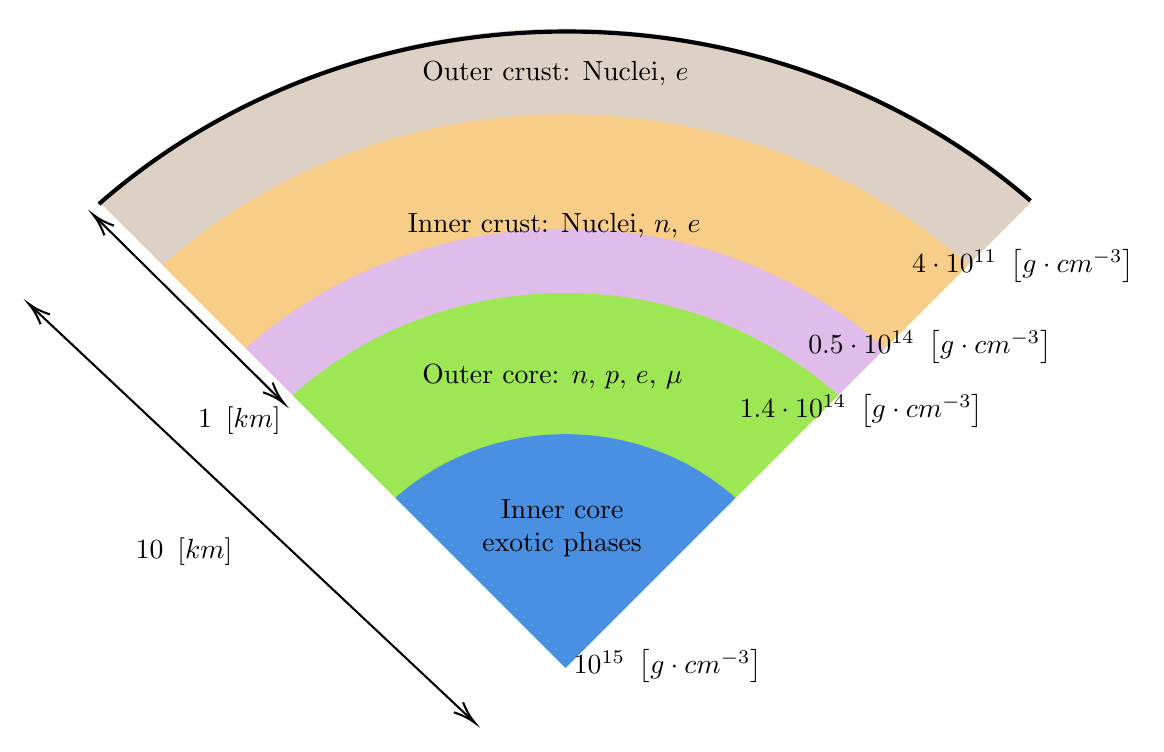
\begin{tikzpicture}[x=0.75pt,y=0.75pt,yscale=-1,xscale=1]
		%uncomment if require: \path (0,1500); %set diagram left start at 0, and has height of 1500
		
		%Shape: Pie [id:dp2707796092987802] 
		\draw  [draw opacity=0][fill={rgb, 255:red, 220; green, 209; blue, 196 }  ,fill opacity=1 ] (85.36,109.52) .. controls (143.85,57.52) and (222.69,25.65) .. (309.43,25.65) .. controls (396.17,25.65) and (475.01,57.52) .. (533.5,109.52) -- (309.43,333.59) -- cycle ;
		%Shape: Pie [id:dp7700324012545914] 
		\draw  [draw opacity=0][fill={rgb, 255:red, 248; green, 205; blue, 135 }  ,fill opacity=1 ] (115.39,139.55) .. controls (166.04,94.52) and (234.32,66.92) .. (309.43,66.92) .. controls (384.55,66.92) and (452.82,94.52) .. (503.47,139.55) -- (309.43,333.59) -- cycle ;
		%Shape: Pie [id:dp8145430572404153] 
		\draw  [draw opacity=0][fill={rgb, 255:red, 223; green, 188; blue, 233 }  ,fill opacity=1 ] (155.47,179.63) .. controls (195.66,143.9) and (249.83,122) .. (309.43,122) .. controls (369.03,122) and (423.2,143.9) .. (463.39,179.63) -- (309.43,333.59) -- cycle ;
		%Shape: Pie [id:dp9495344102501058] 
		\draw  [draw opacity=0][fill={rgb, 255:red, 158; green, 231; blue, 84 }  ,fill opacity=1 ] (178.03,202.19) .. controls (212.33,171.69) and (258.56,153) .. (309.43,153) .. controls (360.3,153) and (406.54,171.69) .. (440.84,202.19) -- (309.43,333.59) -- cycle ;
		%Shape: Pie [id:dp14692440319755318] 
		\draw  [draw opacity=0][fill={rgb, 255:red, 74; green, 144; blue, 226 }  ,fill opacity=1 ] (227.51,251.67) .. controls (248.89,232.65) and (277.72,221) .. (309.43,221) .. controls (341.15,221) and (369.97,232.65) .. (391.36,251.67) -- (309.43,333.59) -- cycle ;
		%Shape: Arc [id:dp6284945559937751] 
		\draw  [draw opacity=0][line width=1.5]  (84.69,110.11) .. controls (142.67,59.3) and (220.71,27.83) .. (306.8,27.02) .. controls (394.39,26.2) and (474.25,57.26) .. (533.5,108.52) -- (309.66,330.03) -- cycle ; \draw  [line width=1.5]  (84.69,110.11) .. controls (142.67,59.3) and (220.71,27.83) .. (306.8,27.02) .. controls (394.39,26.2) and (474.25,57.26) .. (533.5,108.52) ;  
		%Straight Lines [id:da3523350959755407] 
		\draw    (83.29,116.59) -- (172.44,204.78) ;
		\draw [shift={(173.86,206.18)}, rotate = 224.69] [color={rgb, 255:red, 0; green, 0; blue, 0 }  ][line width=0.75]    (10.93,-3.29) .. controls (6.95,-1.4) and (3.31,-0.3) .. (0,0) .. controls (3.31,0.3) and (6.95,1.4) .. (10.93,3.29)   ;
		\draw [shift={(81.86,115.18)}, rotate = 44.69] [color={rgb, 255:red, 0; green, 0; blue, 0 }  ][line width=0.75]    (10.93,-3.29) .. controls (6.95,-1.4) and (3.31,-0.3) .. (0,0) .. controls (3.31,0.3) and (6.95,1.4) .. (10.93,3.29)   ;
		%Straight Lines [id:da7895995544042789] 
		\draw    (52.32,159.55) -- (264.41,358.72) ;
		\draw [shift={(265.86,360.09)}, rotate = 223.2] [color={rgb, 255:red, 0; green, 0; blue, 0 }  ][line width=0.75]    (10.93,-3.29) .. controls (6.95,-1.4) and (3.31,-0.3) .. (0,0) .. controls (3.31,0.3) and (6.95,1.4) .. (10.93,3.29)   ;
		\draw [shift={(50.86,158.18)}, rotate = 43.2] [color={rgb, 255:red, 0; green, 0; blue, 0 }  ][line width=0.75]    (10.93,-3.29) .. controls (6.95,-1.4) and (3.31,-0.3) .. (0,0) .. controls (3.31,0.3) and (6.95,1.4) .. (10.93,3.29)   ;
		
		% Text Node
		\draw (239,40) node [anchor=north west][inner sep=0.75pt]   [align=left] {Outer crust: Nuclei, $\displaystyle e$};
		% Text Node
		\draw (232,113) node [anchor=north west][inner sep=0.75pt]   [align=left] {Inner crust: Nuclei, $\displaystyle n$, $\displaystyle e$};
		% Text Node
		\draw (239,186) node [anchor=north west][inner sep=0.75pt]   [align=left] {Outer core: $\displaystyle n$, $\displaystyle p$, $\displaystyle e$, $\displaystyle \mu $};
		% Text Node
		\draw (263,250.91) node [anchor=north west][inner sep=0.75pt]   [align=left] {\begin{minipage}[lt]{65.08pt}\setlength\topsep{0pt}
		\begin{center}
		Inner core\\exotic phases
		\end{center}
		
		\end{minipage}};
		% Text Node
		\draw (475,130.31) node [anchor=north west][inner sep=0.75pt]    {$4\cdot 10^{11} \ \left[\text{g} \cdot \text{cm}^{-3}\right]$};
		% Text Node
		\draw (425,169.31) node [anchor=north west][inner sep=0.75pt]    {$0.5\cdot 10^{14} \ \left[\text{g} \cdot \text{cm}^{-3}\right]$};
		% Text Node
		\draw (392,200.31) node [anchor=north west][inner sep=0.75pt]    {$1.4\cdot 10^{14} \ \left[\text{g} \cdot \text{cm}^{-3}\right]$};
		% Text Node
		\draw (312,323.31) node [anchor=north west][inner sep=0.75pt]    {$10^{15} \ \left[\text{g} \cdot \text{cm}^{-3}\right]$};
		% Text Node
		\draw (131,206.31) node [anchor=north west][inner sep=0.75pt]    {$1\ \left[\text{km}\right]$};
		% Text Node
		\draw (101,269.31) node [anchor=north west][inner sep=0.75pt]    {$10\ \left[\text{km}\right]$};
		\end{tikzpicture}
		\vspace*{3mm}
		\caption{Neutron star slice}
	\end{figure}
	On the figure below we have an overview of what we expect to be the composition of the inner crust in a neutron star:
	\begin{figure}[H]
		\centering
		\includegraphics[scale=0.9]{img/cosmology/neutron_star_inner_crust.jpg}	
		\caption{Neutron star inner crust}
	\end{figure}
	At lower densities, a lattice of super-heavy, neutron-rich nuclei is immersed in a fluid of neutrons (which are likely to be superfluid) and a relativistic electron gas. At high enough densities the nuclei might deform and connect along certain directions to form extended tubes, sheets and bubbles of nuclear matter. These nuclear pasta phases might form a layer at the base of the neutron star crust, sometimes referred to as the mantle. Ranges of density and thickness given for each layer represent current uncertainties in the physics of neutron star crusts.
	
	\paragraph{Rotation break limit}\mbox{}\\\\\
	Let us make the simplifying assumption that the limit speed of rotation of a star (planet or star) is that which balances the centrifugal force and gravitational force on the surface of the star such that we are led to write (\SeeChapter{see section Classical Mechanics page \pageref{central force}}):
	
	Write this relation supposes obviously that there is no connection other than the gravity which intervenes in the internal cohesion of the star. So the rotational time values we are going to get represent an upper bound (in the sense that the actual value is probably smaller).
	
	It then comes from the previous relation:
	
	To get the rotation time to which it corresponds, it suffices to divide the perimeter at the equator by its speed:
	
	So, for the Earth, we have as limit period of rotation before rupture:
	
	For the Sun:
	
	Let us now consider the case of the pulsar NP0532 which has a rotation of $33$ milliseconds\footnote{In the beginning of the 121st century (holocene calendar) there is a project of NASA of using pulsars as interplanetary GPS.}. We would like to determine its radius. We then have using the previous relations:
	
	Using the theoretical relation of the Chandrasekhar mass limit (since a pulsar is a Neutron star rotating rapidly on itself):
	
	We then have for the radius of the smallest possible pulsar according to these hypotheses (and approximations...):
	
	With the following numerical application (using data from the Crab pulsar):
	
	With the pulsar millisecond PSR J1748-2446ad having a period of 1.39 milliseconds we then fall on\footnote{The slowest know pulsar known at the day we write these lines is PSR J0250+5854 with a rotation period of $23.5$ [s]. The faster pulsar is PSR J1748-2446ad with a rotation period of $0.00139$ [s]}:
	
	what is remarkable (even if it is an approximation!) to think that such a quite huge mass can be contained in such a small radius. Note that for the latter it corresponds to respectively a maximum density of:
	

	\paragraph{Neutron Star Masses and Densities}\mbox{}\\\\\
	 If a nearly spherical star of mass $M$ and radius $R$ rotates with angular velocity $\omega=2\pi/R$ we know obviously that we have then equilibrium of the centrifugal force and gravitational bound a the equator at a given instant such that we are led to write (we make here an obvious classical approximation instead of using General Relativity that should be mandatory when dealing with huge masses):
	
	Hence:
	
	After simplification:
	
	Implying:
	
	Hence:
	
	As the density of a ball is given by:
	
	We then have:
	
	Hence:
	
	That latter relation gives a conservative lower limit to the mean density because a rapidly spinning star is oblate, which increases the centrifugal acceleration and decreases the gravitational acceleration at its equator.

	The first pulsar discovered has a period of $T=1.3$ [s], so its mean density is at least:
	
	The fastest known pulsar actually (year 12018 according to holocene calendar), PSR J1748-2446ad, has $T=1.4\cdot 10^{-3}$ [s] implying $\rho>10^{14}$, the density of atomic nuclei!!!!! It has been calculated that this neutron star contains slightly less than two times the mass of the Sun, within the typical range of neutron stars. Its radius is constrained to be less than $16$ [km]. At its equator it is spinning at approximately $24\%$ of the speed of light, or over $70,000$ [km] per second!!!
	
	\paragraph{Neutron star magnetic field}\mbox{}\\\\\
	As the star's core collapses, its rotation rate increases as a result of conservation of angular momentum, hence newly formed neutron stars rotate at up to several hundred times per second. Some neutron stars emit beams of electromagnetic radiation that make them detectable as pulsars. Indeed, the discovery of pulsars in 11967 (holocen calendar) was the first observational suggestion that neutron stars exist. The radiation from pulsars is thought to be primarily emitted from regions near their magnetic poles. If the magnetic poles do not coincide with the rotational axis of the neutron star, the emission beam will sweep the sky, and when seen from a distance, if the observer is somewhere in the path of the beam, it will appear as pulses of radiation coming from a fixed point in space (the so-called "lighthouse effect"). The fastest rotation rate for a neutron star was a rate of $716$ times a second or $43,000$ revolutions per minute, giving a linear speed at the surface on the order of $0.165 c$....
	
	So now let us focus on the simplified math approach of the impact of the angular momentum conservation on the magnetic field of the star. 
	
	From the conservation of angular moment as the core collapses we have (\SeeChapter{see section Classical Mechanics page \pageref{moment of inertia}}):
	
	Or,  for a sphere of constant density  (\SeeChapter{see section Geometric Shapes page \pageref{inertia momentum ball}}):
	
	So the final spin frequency is:
	
	or the final spin period is:
	
	The magnetic flux $\Phi$ ($\vec{B}$ multiplied by $S$) through the surface of the core is also conserved in collapse. So roughly (\SeeChapter{see section Electrodynamics page \pageref{gauss law for magnetism}}):
	
	Which means that:
	
	The Sun and many other stars are known to possess approximately dipolar magnetic fields. Stellar interiors are fully ionized and hence good electrical conductors. Charged particles are constrained to move along magnetic field lines, and magnetic field lines are tied to the charged particles. When a star collapses from a radius $\sim 10^{6}\; [\text{km}]$ to $\sim 10\; [\text{km}]$, its cross-sectional area $a$ is divided by $\sim 10^{10}$, its magnetic flux $\Phi \equiv \int \vec{B} \cdot \hat{n} \mathrm{d}a$ (where $\hat{n}$ is the unit vector normal to each infinitesimal surface area $\mathrm{d}a$) is conserved, and the magnetic field strength is multiplied by $\sim 10^{10}$. An initial magnetic field strength $B \sim 100$ [G] becomes $B \sim 10^{12}$ [G] after collapse, so young neutron stars should have very strong dipolar fields. The best models of the core-collapse process show that a dynamo effect can generate even stronger magnetic fields. Such dynamos may be able to produce the $10^{14}-10^{15}$ [G] fields observed in magnetars, which are neutron stars having such strong magnetic fields that their radiation is powered by magnetic field decay. Conservation of angular momentum during collapse increases the rotation rate by about the same factor, $10^{10}$, yielding initial rotation periods in the millisecond range.
	
	\paragraph{Spin-Down Luminosity}\mbox{}\\\\\
	If we now consider a neutron star as perfectly symmetric of radius $R=10$ [km] it's moment of inertia will be equal to (\SeeChapter{see section Classical Mechanics page \pageref{moment of inertia}}):
	
	The rotational kinetic energy (\SeeChapter{see section Classical Mechanics page \pageref{moment of inertia}}) of a canonical neutron star with the rotation period $T=0.033$ [s] of the Crab pulsar is:
	
	As magnetic dipole radiation extracts rotational energy, it slowly increases the period of a pulsar:
	
	Note that the period derivative $\dot{T}$ is a dimensionless (seconds per second) pure number. Combining the observed period $T$ and period derivative $\dot{T}$ yields an estimate of the rate $\dot{E}$ at which the rotational energy is changing. The quantity:
	
	is named the "\NewTerm{spin-down luminosity}". It is not a measured luminosity; it is the measured loss rate of rotational energy, which is presumed to equal the luminosity of magnetic dipole radiation. The spin-down luminosity is usually expressed in terms of the pulse period $T$ :
	
	and the prior-previous relation becomes:
	
	The Crab pulsar has $T=0.033$ [s] and $\dot{T}=10^{-12.4}$ (notice that the precision is so that pulsars can be used as galactic GPS!). If $J=10^{38}\; [\text{kg}\cdot \text{m}^{2}]$, its spin-down luminosity is:
	
	So the luminosity of the low frequency magnetic dipole radiation from the Crab pulsar is comparable with the entire radio output of our Galaxy...

	Arrived so far in the study of some very common stars models (excepted for Black Holes that are treated in the section of General Relativity page \pageref{black hole}) it is maybe the right time to introduce this summary image:
	\begin{figure}[H]
		\centering
		\includegraphics[width=1.0\textwidth]{img/cosmology/type_of_stars.jpg}
		\caption[Star comparisons from Black Dwarf to hyper giants]{Star comparisons from Black Dwarf to hyper giants (author: Karl Garnham)}
	\end{figure}
	
	\pagebreak
	\subsection{Galaxies}
	A galaxy is a gravitationally bound system of stars, stellar remnants, interstellar gas, dust, and (of the supposed...) dark matter. 

	Galaxies range in size from dwarfs with just a few billion ($10^9$) stars to giants with one hundred trillion ($10^{14}$) stars, each orbiting its galaxy's center of mass. Galaxies are categorized according to their visual morphology as elliptical, spiral or irregular:
	\begin{figure}[H]
		\centering
		\includegraphics[width=1.0\textwidth]{img/cosmology/classification_galaxies_spitzer.jpg}
		\caption{Apparent stars speed anomaly in galaxies rotations}
	\end{figure}
	 Many galaxies are thought to have Black Holes at their active centers. 

	It seems that there is between $2\cdot 10^{11}$ galaxies in the observable Universe following the actual estimates in this early 121st century (holocene calendar). Most of the galaxies are $1,000$ to $100,000$ parsecs in diameter and usually separated by distances on the order of millions of parsecs (or megaparsecs). The space between galaxies is filled with a tenuous gas having an average density of less than one atom per cubic meter. The majority of galaxies are gravitationally organized into associations known as galaxy groups, clusters, and superclusters. At the largest scale, these associations are generally arranged into sheets and filaments surrounded by immense voids.
	
	\begin{table}[H]
		\centering
		\resizebox{\textwidth}{!}{\begin{tabular}{|l|c|c|c|c|c|c|}
		\hline
		\rowcolor[gray]{0.75} 
		\textbf{Galaxy} & \multicolumn{1}{l|}{\cellcolor[gray]{0.75}\textbf{Type}} & \multicolumn{1}{l|}{\cellcolor[gray]{0.75}\parbox{1.8cm}{\textbf{Distance ($\pmb{10^3}$ {[}LY{]})}}} & \multicolumn{1}{l|}{\cellcolor[gray]{0.75}\parbox{1.8cm}{\textbf{Diameter ($\pmb{10^3}$ {[}LY{]})}}} & \multicolumn{1}{l|}{\cellcolor[gray]{0.75}\parbox{1.8cm}{\textbf{Mass ($\pmb{10^9}\;[\text{M}_\odot]$)}}} & \multicolumn{1}{l|}{\cellcolor[gray]{0.75}\textbf{Abs. Magn.}} & \multicolumn{1}{l|}{\cellcolor[gray]{0.75}\parbox{2cm}{\textbf{Radial speed $\pmb{[\text{km}\cdot\text{s}^{-1}]}$}}} \\ \hline
		Milky Way & Sb & - & $100$ & $150$ & $-20$ & - \\ \hline
		Large Magellanic Cloud & Irr I & $170$ & $23$ & $10$ & $-18.5$ & $+270$ \\ \hline
		Small Magellanic Cloud (NGC 292) & Irr I & $200$ & $10$ & $20$ & $-16.8$ & $+170$ \\ \hline
		Andromeda (NGC 224) & Sb & $2,250$ & $160$ & $300$ & $-21.1$ & $-275$ \\ \hline
		NGC 221 & E 2 & $2,150$ & $3$ & $3$ & $-16.4$ & $-210$ \\ \hline
		NGC 205 & E 1 & $2,100$ & $6$ & $10$ & $-16.4$ & $-240$ \\ \hline
		Triangulum Galaxy (NGC 598) & Sc & $2,250$ & $26$ & $10$ & $-18.9$ & $-190$ \\ \hline
		NGC 147 & E 5 & $2,150$ & $3$ & $1$ & $-14.9$ & $-250$ \\ \hline
		NGC 185 & E 5 & $2,150$ & $3$ & $1$ & $-15.2$ & $-300$ \\ \hline
		IC 1613 & Irr I & $2,400$ & $3$ & $0.3$ & $-14.8$ & $-240$ \\ \hline
		NGC 6822 & Irr I & $1,500$ & $6$ & $0.4$ & $-15.7$ & $-40$ \\ \hline
		Sculptor Galaxy (NGC 253) & E & $280$ & $3$ & $0.003$ & $-11.7$ &  \\ \hline
		Fornax Dwarf & E & $550$ & $6$ & $0.02$ & $-13.6$ & $+40$  \\ \hline
		Leo I & E 4 & $750$ & $3$ & $0.003$ & $-11.0$ &  \\ \hline
		Leo II & E 1 & $750$ & $3$ & $0.001$ & $-9.4$ &  \\ \hline
		Ursa Minor Dwarf & dwarf & $220$ & $3$ & $0.0001$ & $-8.8$ &  \\ \hline
		M82 of Ursa Major (NGC 3034) & Irr II & $10$ & $23$ & $30$ & $-19.5$ & $+400$ \\ \hline
		M81 of Ursa Major (NGC 3031) & Sb & $10$ & $100$ & $200$ & $-21.0$ & $+80$ \\ \hline
		M51 Whirlpool Galaxy (NGC 5194) & Sc & $13$ & $65$ & $80$ & $-19.7$ & $+550$ \\ \hline
		NGC 5128 & E 0p & $16$ & $30$ & $1,000$ & $-20.0$ & $+260$ \\ \hline
		M101 Pinwheel Galaxy  (NGC 5457) & Sc & $20$ & $200$ & $300$ & $-20.0$ & $+400.00$ \\ \hline
		M83 Southern Pinwheel Galaxy (NGC 5236) & SBc & $26$ & $300$ & $1,000$ & $-20.5$ & $+320.0$ \\ \hline
		M104 Sombrero Galaxy (NGC 4594) & Sa & $40$ & $30$ & $500$ & $-22.0$ & $+1,050$ \\ \hline
		M87 Virgo A (NGC 4486) & E 1 & $50$ & $40$ & $300$ & $-22.0$ & $+1,220$ \\ \hline
		\end{tabular}}
		\caption{Data table of some well known galaxies}
	\end{table}
	A small mosaic of some galaxies (without their names) to see that their shape can vary a lot :
	\begin{figure}[H]
		\centering
		\includegraphics[width=0.55\textwidth]{img/cosmology/galaxies_gallery.jpg}
		\caption{Gallery of some galaxies}
	\end{figure}
	Size comparisons of some famous galaxies:
	\begin{figure}[H]
		\centering
		\includegraphics[width=1.0\textwidth]{img/cosmology/galaxies_size_comparison.jpg}
		\caption[Size comparisons of famous galaxies]{Size comparisons of famous galaxies (author: Rhys Taylor)}
	\end{figure}
	
	\subsubsection{Probability of collisions in merging galaxies}
	Stars collide with each other very rarely. The distance between neighbouring stars (at our position in the Milky Way Galaxy) is approximately equal to $10$ million times the diameter of a star. By contrast, galaxies collide with each other quite frequently. The distance between neighbouring galaxies is approximately equal to $20$ times the diameter of a galaxy.

	To illustrate this difference, consider building a scale model of our galaxy in which the stars are represented by ping-pong balls. In this model, the distance between the Sun and Alpha Centauri will be $1,100$ kilometres (the distance between Columbus and Jacksonville, Florida). Now consider a scale model of the universe in which individual galaxies are represented by ping-pong balls. In this model, the Milky Way Galaxy and the Andromeda Galaxy will be a pair of ping-pong balls only 1 meter apart.
	
	Let's see what we get from some back-of-the-envelope estimates.

	Imagine throwing one star (e.g., the Sun) at the other galaxy. How likely is it we'll hit a star in the other galaxy? Well, it's basically proportional to how big a target each star in the other galaxy is (its cross-sectional area) compared to the size of the whole galaxy, multiplied by the total number of stars in the target galaxy.

	Let's assume it's the Milky Way-Andromeda scenario, so each galaxy has about 100 billion stars, and each star is roughly the same size as the Sun (some are much larger, most are smaller). The actual target area for an individual star is a circle with twice the star's radius (we're counting one star just grazing the other as a collision). Let's also assume the stars are more or less evenly distributed in a circular disk. Since "$100,000$ light years" is a common (and not completely crazy) estimate of the Milky Way's size, that's a circle of radius $= 50,000$ light years (about $10^{16}$ meters).

	\begin{figure}[H]
		\centering
		\includegraphics[width=1.0\textwidth]{img/cosmology/colliding_galaxies_ngc_2207.jpg}
		\caption[NGC 2207 is a pair of colliding spiral galaxies]{NGC 2207 is a pair of colliding spiral galaxies (source: NASA/Hubble)}
	\end{figure} 
	
	So, let us consider two galaxies as perfect discs of $100$ billion ($10^{11}$) stars uniformly distributed in the disc going  in the target galaxy, each with target average radius $\sim 2 R_{\odot}$, gives us a total target area of:
	
	The cross-section area of the target galaxy is:
	
	Therefore the probability of a typical average star hitting another star in the other galaxy is :
	
	or about one in a trillion.
	
	The odds of any star from our galaxy not hitting a star in the other galaxy would be:
	
	So there's only about a $10\%$ chance of one (or more) of the galaxy's $100$ billion stars hitting a star in the other galaxy. And the chances of any one particular star (like our Sun) hitting a star in the other galaxy is about one in a trillion.
	\begin{tcolorbox}[title=Remark,arc=10pt,breakable,drop lifted shadow,
  skin=enhanced,
  skin first is subskin of={enhancedfirst}{arc=10pt,no shadow},
  skin middle is subskin of={enhancedmiddle}{arc=10pt,no shadow},
  skin last is subskin of={enhancedlast}{drop lifted shadow}]
	Obviously we could use the binomial law to get the probability (or cumulated probability depending on what we want) that $k$ among $N$ start would get hit:
	
	or as the probabilities are very small and the population huge we could even use a Poisson distribution instead!
	\end{tcolorbox}
	
	\subsubsection{Radial Speed Anomaly}
	In 11978 (holocene calendar), Vera Rubin begins to observe that in galaxies, more the stars are distant from the galactic core, the more their angular velocity is high... The initial observation that uniformity of speed was unexpected because the theory of gravity Newton predicted that more distant objects have less speed. For example, the planets of the solar system orbit with a respective speed decreases while growing their respective distance from the Sun. We are left with the same problem: how to explain a point measurement is greater than the theoretical value?
	\begin{figure}[H]
		\centering
		\includegraphics{img/cosmology/apparent_anomaly_star_speed_galaxy_rotation.jpg}	
		\caption{Apparent stars speed anomaly in galaxies rotations}
	\end{figure}
	According to Newton's laws, in a circular path, there is a as we know balance between the centripetal acceleration and gravitational attraction:
	
	The volume of a disk galaxy of radius $R$ and thickness $e$ is (\SeeChapter{see section Geometric Shapes page \pageref{cylinder}}):
	
	If we consider the mass of the galaxy almost entirely within the radius $R _ {\max}$, corresponding to the maximum speed, of density $\rho$ is given then by:
	
	Making the approximation that the mass is substantially within the range corresponding to the maximum speed, we can write:
	
	Which, introduced into the first equation but rearranged:
	
	 gives:
	
	the law that the maximum speed varies as the $1/4$ power of the mass. After that the speed decrease of the stars should decrease following:
	
	But we must keep in mind that this is a two body relation! In the facts a galaxy should be considered as an isotropic fluid (like the rest of the universe) and therefore it is quite normal that the two-body assumption does not suit the observations. A galaxy can also not be consider as a solid cylinder otherwise by applying $v=\omega r$ the speed of the stars should increase in proportion to the distance to the center of the galaxy. For a more rigorous treatment of the topic the reader should refer to the page \pageref{gravitation disc}.
	
	\begin{flushright}
	\begin{tabular}{l c}
	\circled{90} & \pbox{20cm}{\score{4}{5} \\ {\tiny 28 votes,  80.71\%}} 
	\end{tabular} 
	\end{flushright}

	%to make section start on odd page
	\newpage
	\thispagestyle{empty}
	\mbox{}
	\section{Special Relativity}\label{special relativity}
	\lettrine[lines=4]{\color{BrickRed}W}{e} have always considered until now in all our developments that the interactions (causes and effects) between objects were instantaneous and that the observation of a phenomenon took place therefore instantly after it had occured. However two physicists (Michelson and Morley) during an experiment in 11887 (holocene calendar) discovered something that would change radically all of classical physics: the velocity (speed) of light was invariant (constant) regardless of the movement that we had relatively to it!
	
	This observation is even more important that we know that it is mainly the light that allows us to perceive and feel things around us! It should also be taken into consideration that the electrostatic and magnetic fields are, as we have seen in the section of Quantum Field Theory, carried by the vector of interaction that is the photon that moves at the finite speed of light denoted by $c$. This fact also allows us to assume that the gravitational field also has an interaction vector (which would be the "graviton" whose existence seems indirectly proven but not yet confirmed still in this early 121st century according to holocene calendar) that propagates at the speed of light. It is therefore appropriate to take into account this non-immediacy and the consequences that this entails in the observed phenomena to finally be able to decide what is really of what seems to be.
	
	Before we start with the calculations, we need to define a little bit what will be studied in this section (which applies not only to cosmology but... it seemed to us better to put it in this chapter rather than in the chapter of Mechanics or Atomistic).
	
	\textbf{Definition (\#\thesection.\mydef):} The "\NewTerm{Special Relativity}\index{special relativity}" is a theory confined to isolated inertial frames (Galileans), that is to say, the study of animated frames in a uniform (inertial) rectilinear motion. The reason of this will be given in the statement of Special Relativity principle (see below).
	
	\begin{tcolorbox}[title=Remarks,arc=10pt,breakable,drop lifted shadow,
  skin=enhanced,
  skin first is subskin of={enhancedfirst}{arc=10pt,no shadow},
  skin middle is subskin of={enhancedmiddle}{arc=10pt,no shadow},
  skin last is subskin of={enhancedlast}{drop lifted shadow}]
	\textbf{R1.} Restrict the study to inertial frames of course does not does not prohibit that within these, bodies can be animated of a uniform speed or not (an inertial rocket can have bodies inside itself that have a non-uniform movement)!\\
	
	\textbf{R2.} General Relativity's purpose (see corresponding section at page \pageref{general relativity}) is to take into account non-inertial frames and in any coordinate system by making use of the power of the tensor calculus to be applicable in any type of space (other than flat one!).
	\end{tcolorbox}	
	Special Relativity is mainly based on three important concepts:
	\begin{enumerate}
		\item The invariance postulate of speed of light
		\item The cosmological principle (see below)
		\item The principle of Special Relativity (see below)
	\end{enumerate}
	It is also important to inform the reader that we will use here many concepts seen in the section of Linear Algebra, Tensor Calculus, Trigonometry, Analytical Mechanics, Classical Mechanics, Electrostatics, Magnetostatics and Electrodynamics. It is therefore strongly advised to have covered these topics before at risk of not understanding what follows.
	
	\subsection{Assumptions and Principles}\label{special relativity assumptions and principles}
	Physics laws express relations between the fundamental physical quantities. If the laws of physics are invariant under Galilean referential change as we have seen in the section of Classical Mechanics, it is not necessarily the same for physical quantities! These can transform from Galilean frame to another according to  simple transformation law as we have seen in the section of Classical Mechanics for velocity for example. It is the same in Special Relativity, but we must now consider what we neglected in our study of Galileo's transformations: the time lag is not the same for two observers if the speed of the light is finite, but the concept of time interval is supposed to be kept invariant!
	
	\subsubsection{Postulate of Invariance}\label{postulate of invariance}
	Laboratory measurements (Michelson-Morley experiment as we have already mentioned) have, for a long time, shown that the speed $c$ measured in an inertial frame (straight line and at constant speed) is constant regardless of its speed. Then we are taken to state the postulate of invariance of light: the speed of light (vector for the transport of photons) can neither be added nor subtracted, to the drive speed of the frame in which we measure it (more clearly it means that no matter how fast you move, you will always measure the speed of light as being numerically finite and equal to $c=299,792,458\; [\text{km}\cdot  \text{s}^{-1}]$!).
	
	As corollary the principle of Galilean relativity (\SeeChapter{see section Classical Mechanics page \pageref{Galilean Relativity Principle}}) according to this premise is completely at fault and then we have to develop a new theory that takes into account of this property of light.
	
	\begin{tcolorbox}[title=Remark,arc=10pt,breakable,drop lifted shadow,
  skin=enhanced,
  skin first is subskin of={enhancedfirst}{arc=10pt,no shadow},
  skin middle is subskin of={enhancedmiddle}{arc=10pt,no shadow},
  skin last is subskin of={enhancedlast}{drop lifted shadow}]
	It is important to notice that we consider that light, within the framework of Special Relativity, the messenger of information from one body to another, that is to say the speed of causality effect!!!
	\end{tcolorbox}
	On Internet Forums a common and interesting question is: \textit{Why is there a limit speed for causality and for the speed of light?}
	
	First, if the light speed would be infinite, we would not have light at all! Indeed, to see this, take a look at Maxwell's equations again, Note that in them we have the factor:
	
	so if we set $c\rightarrow +\infty$ then either (or both) of $\mu_0$ and $\varepsilon_0$ would have to be zero. This will effectively kill the existence of dynamic magnetic fields.

	Especially, for light, it means that:
	
	So, magnetic fields would be static (and of zero intensity, remember no magnetic monopoles known so far!). Thus the only thing left of electromagnetism would be simply electrostatics. Physically this also make sense, if $c\rightarrow +\infty$ the electric field response to any rearrangement of charges would be instantaneous, so there is no place (time?) for a magnetic field response.
	
	The existence of the speed limit for causality is related to the existence of time itself. Indeed, if there would be no speed limit, everything would happen instantly (as well as distance and consequently space by the way). It is difficult to imagine a Universe that evolve instantaneously. This is why we belong to a Universe where there is a speed limit otherwise we would very likely not be here to observe it...
	
	\subsubsection{Cosmological Principle}
	We assume that our position in the Universe is typical not only in space as stated in the standard model of the Universe (\SeeChapter{see section Cosmogony page \pageref{newtonian cosmological models}}), but also in time. Thus, an astronomer located in a remote galaxy must observe the same general properties of the Universe that we do whatever he lived a billion years ago or that he observed the Universe in a billion years in the future!
	
	In fact, it is quite natural to go further and state that: the Universe looks the same in every point, that is to say, it is homogeneous. This homogeneity is therefore sets as the "\NewTerm{Cosmological Principle}\index{cosmological principle}".
	
	This principle is not based, still actually in this early 121st century (holocene calendar), on experimental data because they are too much fragmentary compared to the huge size of the cosmos (very likely infinite). Therefore we are not able yet to establish its validity. It constitutes however a presupposition for any physical study of our Universe. Its purpose is relative to its character, essential to any scientific cosmology study, and perhaps to a certain reaction to the geocentric or heliocentric old vision: it is assumed now that no place is special in the cosmos!
	
	For an in-deep discussion and criticism of the subject based on the earliest experimental data (of this early 121st century according to holocene calendar), the reader can refer to the excellent 100 pages paper \textit{Is the observable Universe consistent with the cosmological principle?} (see \cite{aluri2023observable}).
	
	\subsubsection{Special Relativity Principle}\label{special relativity principle}
	Let us remind (\SeeChapter{see section Classical Mechanics page \pageref{Galilean Relativity Principle}}) that the Galilean transformations tell us that no reference frames can be considered as an absolute frame because the relations between the physical quantities are identical in all Galilean repositories ("Galilean relativity principle"). The Galilean motion is therefore relative!
	
	In the 120th century (holocene calendar) physicists noted that an important class of physical phenomena violated the Galilean relativity principle: the electromagnetic phenomena!
	
	By applying the Galilean transformations to Maxwell's equations, we get a different set of equations depending on whether the observer is in a fixed reference or a mobile reference frame.
	
	Indeed, we have proved in the section on Electrodynamics that the electric or magnetic field propagation equation could be written in one-dimensional space as the following d'Alembert equation (see page \pageref{alembertian}):
	
	where $\psi$ represents any one of the two fields (electric or magnetic). We name this relation sometimes "\NewTerm{Hertz equation}\index{Hertz equation}".
	
	We also saw in the section of Classical Mechanics (see page \pageref{Galilean Relativity Principle}) that an important factor in the validity of a theory is the invariance of the expression of its laws under a Galilean transformation by putting:
	
	We have also shown in the section of Differential and Integral Calculus (see page \pageref{total exact differential}) that the total differential of a function was written (example with two variables):
	
	Therefore:
	
	Which brings us to simply write (using the physicist method way of life...):
	
	After elimination of $f$ and using the Schwarz theorem (\SeeChapter{see section Differential and Integral Calculus page \pageref{Schwarz theorem}}) and still the physicist way of life:
	
	If we write the same with the time variable:
	
	Ultimately the Galilean transformation of the wave equation supposedly have an invariant form becomes:
	
	To fix the situation, following this example, we can state at least three assumptions:
	\begin{enumerate}
		\item[H1.] Maxwell's equations are false. The correct equations remain to be discovered and must be invariant under a Galilean transformation.
		
		\item[H2.] Galilean invariance is valid for mechanics but not for electromagnetism (that was the historical solution before Albert Einstein: an "ether" determines the existence of a kind of absolute repository where Maxwell's equations didn't change).
		
		\item[H3.] Galilean invariance is false. There is a more general invariance, it remains to be discovered, which preserves the form of the Maxwell equations. Classical mechanics is to be reformulated so that it is invariant under this new transformation.
	\end{enumerate}
	\begin{tcolorbox}[title=Remark,arc=10pt,breakable,drop lifted shadow,
  skin=enhanced,
  skin first is subskin of={enhancedfirst}{arc=10pt,no shadow},
  skin middle is subskin of={enhancedmiddle}{arc=10pt,no shadow},
  skin last is subskin of={enhancedlast}{drop lifted shadow}]
	It turns out that the first two assumptions are excluded by the experimental facts. Moreover, Maxwell's equations integrating the speed of light they are implicitly relativistic.
	\end{tcolorbox}	
	Albert Einstein did not accept the violation of the Galilean relativity principle by electromagnetism. From his perspective, it was necessary to generalize it to all natural laws.
	
	He postulated that the laws of physics should be the same in all repositories Galileans, which means, implicitly, that in the point of view of physical laws, it is not possible to distinguish one from another Galilean frame. This result is most commonly formulated as: no reference is privileged. This principle was named "\NewTerm{principle of relativity}\index{principle of relativity}". Indeed, this relativity is restricted to the case of Galileans frames (also named "inertial frames") exclusively.
	
	In other words, the physic laws should remain unchanged after a change of reference. We must therefore identify new adequate transformations that will substitute to the Galilean transformations.
	
	In the case of non Galileans frames repositories are not indistinguishable anymore. Indeed, imagine a person in a train moving at a constant speed and another person on land. Everyone can then say that it is the other who is in motion (relative) and indiscriminately. By cons, if the train begins to accelerate, although the two individuals can say that this is another speeding, only the one on the train will feel the effect of this acceleration ... and repositories are no more indistinguishable.
	
	Albert Einstein abolished as well as the idea that there is an absolute reference point that does not move and on which we can define an absolute time, an absolute length or absolute mass. However, one can define a privileged reference point for every object in the Universe. It is the frame moving at the same speed and in the same direction as the object. The time measured in this privileged reference frame is minimal and is named the "\NewTerm{proper time}\index{proper time}". Similarly, the size of the object is maximum, it is his "\NewTerm{proper dimension}\index{proper dimension}" or "\NewTerm{proper distance}\index{proper distance}", and its mass is minimal, it is its "\NewTerm{proper mass}\index{proper mass}" (we will do the corresponding detailed mathematical developments further below).
	
	\begin{tcolorbox}[title=Remark,arc=10pt,breakable,drop lifted shadow,
  skin=enhanced,
  skin first is subskin of={enhancedfirst}{arc=10pt,no shadow},
  skin middle is subskin of={enhancedmiddle}{arc=10pt,no shadow},
  skin last is subskin of={enhancedlast}{drop lifted shadow}]
	Albert Einstein did share the credit with Hendrik Lorentz and Henri Poincaré for Special Relativity for a while, probably one reason his Nobel prize did not mention relativity. Because Lorentz in 11904 according to holocene calendar (who misinterpreted his own transformations as applying to the Ether) laid the fundamentals for the work by Einstein, this theory was originally named the "Lorentz–Einstein theory". Poincaré struggled with his own proof of $E=3/4 mc^2$ and improved Lorentz transformation formulation (June 5, 11905 according to holocene calendar). Einstein at the very least gets credit for being the first to correctly interpret the equations and do away with the Ether concept and get the correct relation $E=mc^2$ (June 30, 11905 according to holocene calendar).
	\end{tcolorbox}	
	
		\subsection{Lorentz Transformations/Boost}\label{lorentz transformations}
		For make possible to $c$ to be invariant (light speed invariance postulate), we must admit that time appears to not flow the same way for the observer $\text{O}$ that is motionless than for the observer $\text{O}'$ in a reference frame in uniform translation (i.e.: an inertial frame) in the direction of $x$  with relative velocity (the term "relative" is important!) $v$ (caution! the relative speed between the repositories is often denoted in the literature by $u$).

		\begin{tcolorbox}[title=Remark,arc=10pt,breakable,drop lifted shadow,
  skin=enhanced,
  skin first is subskin of={enhancedfirst}{arc=10pt,no shadow},
  skin middle is subskin of={enhancedmiddle}{arc=10pt,no shadow},
  skin last is subskin of={enhancedlast}{drop lifted shadow}]
		A special case of disposal of referential frames in which the space axes are parallel leads to what we name the "\NewTerm{pure Lorentz transformations}\index{pure Lorentz transformations}" or "\NewTerm{special Lorentz transformations}\index{special Lorentz transformations}" and the relative displacement along a particular axis is often named a "\NewTerm{boost}\index{boost}".
		\end{tcolorbox}	
		
		To study the behaviour of physic laws, we must bring two clocks that give the times $t$ and $t'$ (the referential frame that contains its clock/measuring instrument is named "\NewTerm{proper referential}\index{proper referential}" or "\NewTerm{proper frame}\index{proper frame}").
		
		Let's set up the following imaginary experiment:
		
		When the observers $\text{O}$ and $\text{O'}$ are superimposed, we set $t = 0$ and $t' = 0$ (clock time sync) and we emit a bright flash\footnote{In fact we should consider the emission of "an element of information". Using light as an example is just convenient for pedagogical purposes. As we will see the results we will get further below involve a speed limit $c$ that is for sure the speed of light, but in reality we should consider light as a special case of the maximum possible speed of information transfer. The "$c$" can then be seen as the "causality speed".} in the direction of a point $A$ spotted by respectively $\vec{r}$ and $\vec{r}^{\,\prime}$:
		\begin{figure}[H]
			\centering
			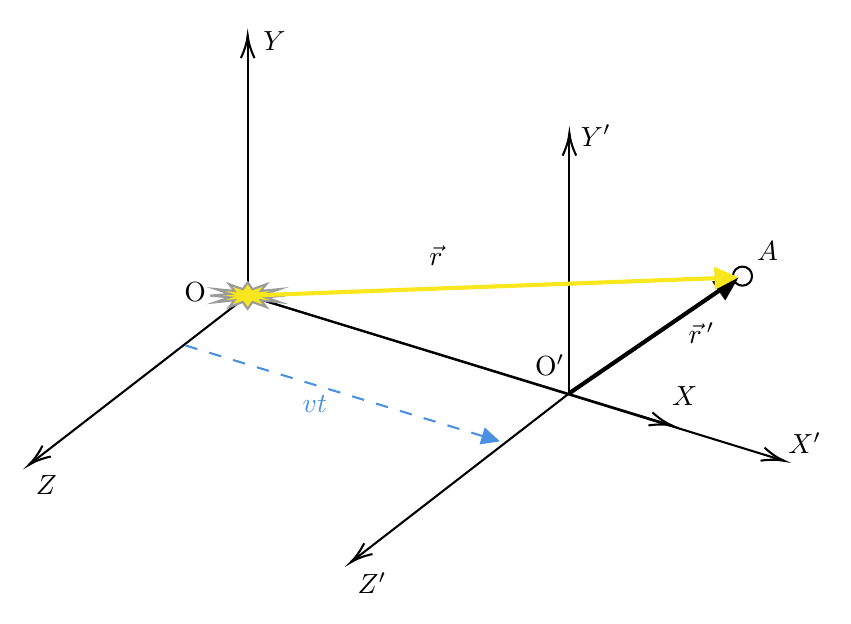
\begin{tikzpicture}[x=0.75pt,y=0.75pt,yscale=-1,xscale=1]
			%uncomment if require: \path (0,825); %set diagram left start at 0, and has height of 825
			
			%Straight Lines [id:da15000187622617145] 
			\draw    (236,181) -- (236,57.6) ;
			\draw [shift={(236,55.6)}, rotate = 90] [color={rgb, 255:red, 0; green, 0; blue, 0 }  ][line width=0.75]    (10.93,-3.29) .. controls (6.95,-1.4) and (3.31,-0.3) .. (0,0) .. controls (3.31,0.3) and (6.95,1.4) .. (10.93,3.29)   ;
			%Straight Lines [id:da7391133173163476] 
			\draw    (391,228) -- (391,104.6) ;
			\draw [shift={(391,102.6)}, rotate = 90] [color={rgb, 255:red, 0; green, 0; blue, 0 }  ][line width=0.75]    (10.93,-3.29) .. controls (6.95,-1.4) and (3.31,-0.3) .. (0,0) .. controls (3.31,0.3) and (6.95,1.4) .. (10.93,3.29)   ;
			%Straight Lines [id:da35796515703202303] 
			\draw    (236,181) -- (492.59,260.01) ;
			\draw [shift={(494.5,260.6)}, rotate = 197.12] [color={rgb, 255:red, 0; green, 0; blue, 0 }  ][line width=0.75]    (10.93,-3.29) .. controls (6.95,-1.4) and (3.31,-0.3) .. (0,0) .. controls (3.31,0.3) and (6.95,1.4) .. (10.93,3.29)   ;
			%Straight Lines [id:da6662748177038846] 
			\draw    (236,181) -- (438.59,243.01) ;
			\draw [shift={(440.5,243.6)}, rotate = 197.02] [color={rgb, 255:red, 0; green, 0; blue, 0 }  ][line width=0.75]    (10.93,-3.29) .. controls (6.95,-1.4) and (3.31,-0.3) .. (0,0) .. controls (3.31,0.3) and (6.95,1.4) .. (10.93,3.29)   ;
			%Straight Lines [id:da41386254054045435] 
			\draw    (236,181) -- (132.08,261.38) ;
			\draw [shift={(130.5,262.6)}, rotate = 322.28] [color={rgb, 255:red, 0; green, 0; blue, 0 }  ][line width=0.75]    (10.93,-3.29) .. controls (6.95,-1.4) and (3.31,-0.3) .. (0,0) .. controls (3.31,0.3) and (6.95,1.4) .. (10.93,3.29)   ;
			%Straight Lines [id:da7881076801433373] 
			\draw    (391,228) -- (287.08,308.38) ;
			\draw [shift={(285.5,309.6)}, rotate = 322.28] [color={rgb, 255:red, 0; green, 0; blue, 0 }  ][line width=0.75]    (10.93,-3.29) .. controls (6.95,-1.4) and (3.31,-0.3) .. (0,0) .. controls (3.31,0.3) and (6.95,1.4) .. (10.93,3.29)   ;
			%Straight Lines [id:da3883244787142972] 
			\draw [color={rgb, 255:red, 74; green, 144; blue, 226 }  ,draw opacity=1 ] [dash pattern={on 4.5pt off 4.5pt}]  (206,205) -- (326.35,241.7) -- (354.63,250.32) ;
			\draw [shift={(357.5,251.2)}, rotate = 196.96] [fill={rgb, 255:red, 74; green, 144; blue, 226 }  ,fill opacity=1 ][line width=0.08]  [draw opacity=0] (8.93,-4.29) -- (0,0) -- (8.93,4.29) -- cycle    ;
			%Straight Lines [id:da3425508680903211] 
			\draw [color={rgb, 255:red, 0; green, 0; blue, 0 }  ,draw opacity=1 ][line width=1.5]    (391,228) -- (469.2,174.46) ;
			\draw [shift={(472.5,172.2)}, rotate = 145.6] [fill={rgb, 255:red, 0; green, 0; blue, 0 }  ,fill opacity=1 ][line width=0.08]  [draw opacity=0] (11.61,-5.58) -- (0,0) -- (11.61,5.58) -- cycle    ;
			%Shape: Circle [id:dp5534520562104084] 
			\draw   (469.8,171.6) .. controls (469.8,169.06) and (471.86,167) .. (474.4,167) .. controls (476.94,167) and (479,169.06) .. (479,171.6) .. controls (479,174.14) and (476.94,176.2) .. (474.4,176.2) .. controls (471.86,176.2) and (469.8,174.14) .. (469.8,171.6) -- cycle ;
			%Shape: Star [id:dp08776025241886987] 
			\draw  [color={rgb, 255:red, 155; green, 155; blue, 155 }  ,draw opacity=1 ][fill={rgb, 255:red, 248; green, 231; blue, 28 }  ,fill opacity=1 ] (236,174.6) -- (238.33,177.91) -- (245,175.46) -- (242.36,178.74) -- (251.59,177.8) -- (244.69,180.17) -- (254,181) -- (244.69,181.83) -- (251.59,184.2) -- (242.36,183.26) -- (245,186.54) -- (238.33,184.09) -- (236,187.4) -- (233.67,184.09) -- (227,186.54) -- (229.64,183.26) -- (220.41,184.2) -- (227.31,181.83) -- (218,181) -- (227.31,180.17) -- (220.41,177.8) -- (229.64,178.74) -- (227,175.46) -- (233.67,177.91) -- cycle ;
			%Straight Lines [id:da0461746867695636] 
			\draw [color={rgb, 255:red, 248; green, 231; blue, 28 }  ,draw opacity=1 ][line width=1.5]    (236,181) -- (468.5,172.35) ;
			\draw [shift={(472.5,172.2)}, rotate = 177.87] [fill={rgb, 255:red, 248; green, 231; blue, 28 }  ,fill opacity=1 ][line width=0.08]  [draw opacity=0] (11.61,-5.58) -- (0,0) -- (11.61,5.58) -- cycle    ;
			
			% Text Node
			\draw (204,173) node [anchor=north west][inner sep=0.75pt]   [align=left] {O};
			% Text Node
			\draw (373,208) node [anchor=north west][inner sep=0.75pt]   [align=left] {O$'$};
			% Text Node
			\draw (242,52.4) node [anchor=north west][inner sep=0.75pt]    {$Y$};
			% Text Node
			\draw (395,97.4) node [anchor=north west][inner sep=0.75pt]    {$Y'$};
			% Text Node
			\draw (439,223.4) node [anchor=north west][inner sep=0.75pt]    {$X$};
			% Text Node
			\draw (495,245.4) node [anchor=north west][inner sep=0.75pt]    {$X'$};
			% Text Node
			\draw (132.5,266) node [anchor=north west][inner sep=0.75pt]    {$Z$};
			% Text Node
			\draw (287.5,313) node [anchor=north west][inner sep=0.75pt]    {$Z'$};
			% Text Node
			\draw (261,227.4) node [anchor=north west][inner sep=0.75pt]  [color={rgb, 255:red, 74; green, 144; blue, 226 }  ,opacity=1 ]  {$vt$};
			% Text Node
			\draw (322,155.4) node [anchor=north west][inner sep=0.75pt]    {$\vec{r}$};
			% Text Node
			\draw (447,192.4) node [anchor=north west][inner sep=0.75pt]    {$\vec{r} \,'$};
			% Text Node
			\draw (480,153.4) node [anchor=north west][inner sep=0.75pt]    {$A$};
			
			\end{tikzpicture}
			\vspace*{3mm}	
			\caption{Configuration for the study of relativistic effects}
		\end{figure}
		It is obvious that when the flash arrive in $A$, the observer $\text{O}$ will measure a time $t$ and $\text{O}'$ a time $t'$.
		
		The observer $\text{O}$ therefore concludes:
		
		The observer $\text{O}'$ therefore concludes:
		
		Since the displacement of $\text{O}'$ is made only along the $\text{O}x$ axis, we have for the two observers:
		
		Moreover, if the path of the light beam coincides within the axe $\text{O}x$, we have:
		
		This gives us then:
		
		And therefore:
		
		these two relations are equal (zero) at any $x, x', t, t'$ between the two observers. These are the first "relativistic invariant" (equal values regardless of the frame), especially here is about the "\NewTerm{invariant interval}\index{invariant interval}" also named "\NewTerm{space-time interval}\index{space-time  interval}", that we find in a more generalized form when applied to the whole space:
		
		Now it should be remembered that in the classical model (Galilean relativity), we would have written that the position of point $A$ for the observer $\text{O}$ from the information given by $\text{O}'$ would be given by $x=x'+vt$ and vice versa (\SeeChapter{see section Classical Mechanics page \pageref{Galilean Relativity Principle}}) such as:
		
		In the relativistic model, we must admit that time $t$ which is related to $x$ is not the same as $t'$ which is related to $x'$, relativity principle oblige (otherwise it would be difficult to explain the invariance of the speed of light)!
		
		We are then led to try to write the above relation as follows:
		
		where $\lambda$ would be a numerical value to be determined from a given algebraic expression. Because to explain the constancy of the speed of light one possibility is that the space must constantly adjust according to our velocity $v$. What is revolutionary hypothesis as we have already mentioned!
	\begin{tcolorbox}[title=Remark,arc=10pt,breakable,drop lifted shadow,
  skin=enhanced,
  skin first is subskin of={enhancedfirst}{arc=10pt,no shadow},
  skin middle is subskin of={enhancedmiddle}{arc=10pt,no shadow},
  skin last is subskin of={enhancedlast}{drop lifted shadow}]
	A reader asked us why we could not write the last relation in the following simplified form (using the relation $x = ct$ obtained above) where point $A$ is on the $X$ axis:
	
	The only reason is that later we will introduce a vector (matrix) notation of this result showing the concept of quadrivector (four-vector) and that it is in the first form of writing (this making explicit reference to time) that we can clearly make the concept of space-time emerge.
	\end{tcolorbox}
	Furthermore, if $t\neq t'$, we must also be able to express $t'$ as a function of $t$ and $x$ in a similar way:
	
	Let us summarize the shape of the problem:
	
	with $\lambda$ to be determined and after:
	
	with $a,b$ to be determined.
	We then seek to determine the relation that gives us to know the values of the coefficients $a$,$b$ and $\lambda$ that satisfy simultaneously:
	
	Remembering the previous developments and bearing in mind that in our special case $y '= y $and $z' = z$, the last equation becomes:
	
	Let us distribute:
	
	To satisfy the relation:
	
	We must have:
	
	It is easy to solve (2):
	
	We then introduce this result in (1) and (3) and we arrive at:
	
	If we divide (1') by (2'), we get:
	
	and introducing this latter result into the relation:
	
	we obtain the following remarkable result:
	
	That we frequently denote by:
	
	and which we name "\NewTerm{Michelson-Morley factor}\index{Michelson-Morley factor}\label{michelson morley factor}" with:
	
	Also introducing:
	
	in:
	
	we get:
	
	Let us write now (to comply with the traditional notations in this field):
	
	with therefore the parameter:
	
	
	\begin{tcolorbox}[enhanced,colback=red!5!white,colframe=black!50!red,boxrule=1pt,arc=0pt,outer arc=0pt,drop lifted shadow,after skip=10pt plus 2pt]
	\bcbombe Caution! The "Lorentz transformations" are sadly sometimes interpreted by scientifically illiterate people and undergraduate students as a physical transformation. But it is not! It's just a mathematical transformation to explain what one reference frame sees in comparison of another one. Nothing more!
	\end{tcolorbox}

	\subsubsection{Displacement four-vector}
	We just derived the "\NewTerm{Lorentz transformation}\index{Lorentz transformation}" relations to pass from the values measured by $\text{O}'$ to those measured in $\text{O}$ and vice versa\footnote{Such relations were first written by Woldemart Voigt in 11887 (holocene calendar). Between 11892 (holocene calendar) and 11902 (holocene calendar) by trial and errors Hendrik Lorentz will improve the shape of these relations. In 11905 (holocene calendar) Poincaré confirmed and corrected Lorent'z work of 11904 (holocene calendar) and give them their definitive shape.}:
	
	That have for property to be covariant (that is to say their relations keep the same structure during a change of a Galilean reference system). We see through these relations that the concept of "time" is something individual relating to the movement we have over other (this is the "\NewTerm{proper time}"). This is why it is not possible to define a "common time" between two people moving relatively and who don't know their respective relative speed (and even here we do not take into account the gravity that distorts space-time ... that we will study in the section of General Relativity).
	\begin{tcolorbox}[title=Remark,arc=10pt,breakable,drop lifted shadow,
  skin=enhanced,
  skin first is subskin of={enhancedfirst}{arc=10pt,no shadow},
  skin middle is subskin of={enhancedmiddle}{arc=10pt,no shadow},
  skin last is subskin of={enhancedlast}{drop lifted shadow}]
	If $v$ is much smaller than $c$, we fall back on the Galilean transformation as $\gamma\cong 1$ and $v/c^2\cong 0$
	\end{tcolorbox}
	We can also write the last relations in a more useful way (the reader will notice that this time that for all relations the units of all the terms to the left of equality are the same: it is every time a distance!):
	
	Of course the difference is that the fourth dimension being the time coordinate of "space-time" seems at the contrary of the spatial coordinates to have a privileged direction: the "\NewTerm{arrow of time}\index{arrow of time}" (you can not go back to a given moment time given in the reality - as least as far as we know today - when it is possible when we traverse a purely spatial distance). The direction of time is imposed by the second law of thermodynamics as entropy can only increase (\SeeChapter{see section Thermodynamics page \pageref{entropy}}). If this were not the case then all time could already exist and we could travel in time as we travel on distances and therefore the future should be already written (people that believe in destiny like this...) and we could also go back in time.... However, thermodynamics does not give a particular direction to the time ... so if our time has the direction it has today.... it is because our universe was organized at its beginning (so it had a low entropy).
	
	By proceeding in a homogenisation of units to be able to use more modern and generalized maths than just simple algebra we can see that in fact when we travel in time we travel in physical point of view a distance $ct$. But because $c$ and $t$ are measured in arbitrary human being units physicists prefer to put $c=1$ we mathematical development become more complicate rather than changing the definition of time.
	
	Now we can put the Lorentz transformations of coordinate and time in the traditional following matrix form (\SeeChapter{see section Linear Algebra page \pageref{linear algebra}}) which defines the "\NewTerm{Lorentz matrix}\index{Lorentz matrix}" or "\NewTerm{Lorentz-Poincare matrix}\index{Lorentz-Poincare matrix}" or "\NewTerm{Lorentz boost}\index{Lorentz boost}\label{lorentz boost tensor}":
	
	and reciprocally:
	
	and the reader can very easily control that with the two previous relations we fall back on:
	
	We have also obviously:
	
	In index form the matrix formulation is written:
	
	which can therefore be written in tensor (\SeeChapter{see section Tensor Calculus page \pageref{tensor notation}}) form:
	
	\begin{tcolorbox}[title=Remark,arc=10pt,breakable,drop lifted shadow,
  skin=enhanced,
  skin first is subskin of={enhancedfirst}{arc=10pt,no shadow},
  skin middle is subskin of={enhancedmiddle}{arc=10pt,no shadow},
  skin last is subskin of={enhancedlast}{drop lifted shadow}]
	We can see the tensor (the matrix) of Lorentz transformation in some books in the condensed form $L(\beta)$ and sometimes $L_\nu^\mu$ or even $\Lambda_\nu^\mu$.
	\end{tcolorbox}
	The vector\label{four-vector displacement}:
	
	is named "\NewTerm{space-time four-vector}\index{space-time four-vector}" or "\NewTerm{four-vector displacement}\index{four-vector displacement}".
	
	Notice that since:
	
	the transformation by the matrix $L_\nu^\mu$ conserves the norm (Lorentz invariance\label{lorentz invariance}). In geometric terms it is thus a "\NewTerm{isometry}\index{isometry}" or an invariance of the dot product by Lorentz transformation.
	
	Let us prove this explicitly following the request of a reader! We will take again for the proof only a movement along $x$ and we use:
	
	As $y'=y$ and $z'=z$ to simplify the development we will ignore these both components.
	
	We will also put to simplify $c=1$ and therefore $v$ is expressed in percentage of $c$ and becomes $v=\beta$:
	
	Now we calculate:
	
	and as $\gamma^2(1-\beta^2)=1$ we get indeed:
	
	
	\paragraph{Wave Equation Invariance}\mbox{}\\\\\
	Now that we have determined the Lorentz transformations, we can check whether the wave equation is invariant with respect to the latter (remember that we have proven earlier that it was not invariant under a Galilean transformation!!!).
	
	Starting from the Lorentz transformation written in explicitly:
	
	we calculate the partial derivatives with respect to $x$ and $t$ (the expression after the second equality has already been proven earlier in this section):
	
	These relation can also be written:
	
	Squared:
	
	In the Maxwell's equations, or rather in the propagation equation of the electric or magnetic field in vacuum, we have proven (\SeeChapter{see section Electrodynamics page \pageref{electromagnetic wave equation}}) that the following operator appeared:
	
	Substituting in it the previous differential expressions:
	
	We therefore have well:
	
	which shows that a Lorentz transformation leaves invariant this operator (Jackpot!). So we got what we were looking for (the wave equation but in the other reference frame)!

	The reader will also have noticed that this only works if and only if the wave propagation speed is the speed of light!

	\paragraph{Hypergeometric interpretation}\mbox{}\\\\\
	Now let us come back to our Lorentz transformations. Let us recall that we have restricted ourselves to the special case where the space axes were parallel (what brought us to define the "pure Lorentz transformations"). This special configuration has an interesting geometric property that sometimes many books use.

	Let us see what this is about:
	
	We have seen in the context of the study of the Lorentz transformations of lengths that we had a special transformation (boost) along one axis, ie the $x$-axis, requiring in this case for the other components:
	
	This allows us to  reduce the transformation matrix $L_\nu^\mu$ ($4\times 4$ matrix that we obtained earlier above) to a $2\times 2$ matrix of components $A$, $B$, $C$ and $D$ such that:
	
	We notice that the components $A$, $B$, $C$, $D$ respect by construction the following expressions:
	
	The first relation can be related with the remarkable identity in hyperbolic trigonometry (\SeeChapter{see section Trigonometry page \pageref{hyperbolic trigonometry}}):
	
	And therefore:
	
	and the second relation that there exists $\alpha_2$ such that:
	
	\begin{tcolorbox}[title=Remark,arc=10pt,breakable,drop lifted shadow,
  skin=enhanced,
  skin first is subskin of={enhancedfirst}{arc=10pt,no shadow},
  skin middle is subskin of={enhancedmiddle}{arc=10pt,no shadow},
  skin last is subskin of={enhancedlast}{drop lifted shadow}]
	The choice of the "$-$" sign for $B$ and $C$ is useful because as we always have $\beta \geq 0$ (same for $\gamma$ that is strictly positive) it will impose us at the end of the calculations to have $\alpha\geq 0$. Therefore, as $-\gamma\beta\leq 0$ and $\alpha\geq 0$ the only way for $C$ (and also for $B$) to be negative is to put a "$-$" sign.
	\end{tcolorbox}	
	The third then gives the remarkable addition relation:
	
	and therefore the difference $\alpha_1-\alpha_2$, that we will denote more simply by $\alpha$, is equal zero. Which validates the relations:
	
	The matrix is therefore presented as follow:
	
	This is (by analogy to the classical one) a "\NewTerm{hyperbolic rotation matrix}\index{hyperbolic rotation matrix}\label{hyperbolic rotation matrix}". We will not go further on this analogy as it is not used for practical cases study in this book.
	
	Finally, the special Lorentz transformation of velocity $v$ along the $x$-axis can also be written:
	
	which brings us to write:
	
	The dimensionless quantity $\alpha$ is named "\NewTerm{rapidity}\index{rapidity}" by those who use physics in high energy. The advantage of working with angles is to make the combination of $2$ boosts easier.
	
	\subsubsection{Velocity four-vector}\label{four vector velocity}
	We can also determine the Lorentz transformations for speed. Let us consider again a particle moving in an inertial reference frame O' such that at time $t'$, its coordinates are $(x ', y', z ').$:
	\begin{figure}[H]
		\centering
		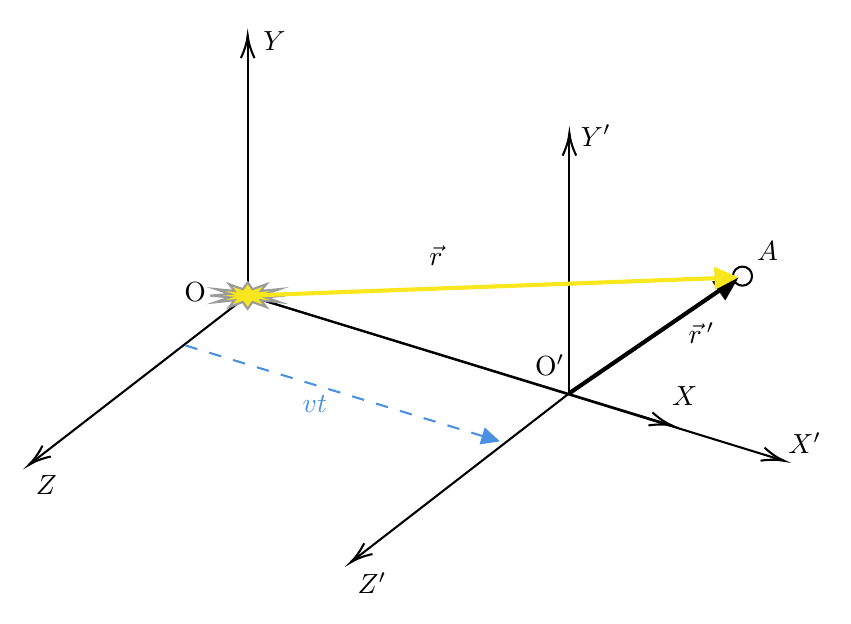
\begin{tikzpicture}[x=0.75pt,y=0.75pt,yscale=-1,xscale=1]
		%uncomment if require: \path (0,825); %set diagram left start at 0, and has height of 825
		
		%Straight Lines [id:da15000187622617145] 
		\draw    (236,181) -- (236,57.6) ;
		\draw [shift={(236,55.6)}, rotate = 90] [color={rgb, 255:red, 0; green, 0; blue, 0 }  ][line width=0.75]    (10.93,-3.29) .. controls (6.95,-1.4) and (3.31,-0.3) .. (0,0) .. controls (3.31,0.3) and (6.95,1.4) .. (10.93,3.29)   ;
		%Straight Lines [id:da7391133173163476] 
		\draw    (391,228) -- (391,104.6) ;
		\draw [shift={(391,102.6)}, rotate = 90] [color={rgb, 255:red, 0; green, 0; blue, 0 }  ][line width=0.75]    (10.93,-3.29) .. controls (6.95,-1.4) and (3.31,-0.3) .. (0,0) .. controls (3.31,0.3) and (6.95,1.4) .. (10.93,3.29)   ;
		%Straight Lines [id:da35796515703202303] 
		\draw    (236,181) -- (492.59,260.01) ;
		\draw [shift={(494.5,260.6)}, rotate = 197.12] [color={rgb, 255:red, 0; green, 0; blue, 0 }  ][line width=0.75]    (10.93,-3.29) .. controls (6.95,-1.4) and (3.31,-0.3) .. (0,0) .. controls (3.31,0.3) and (6.95,1.4) .. (10.93,3.29)   ;
		%Straight Lines [id:da6662748177038846] 
		\draw    (236,181) -- (438.59,243.01) ;
		\draw [shift={(440.5,243.6)}, rotate = 197.02] [color={rgb, 255:red, 0; green, 0; blue, 0 }  ][line width=0.75]    (10.93,-3.29) .. controls (6.95,-1.4) and (3.31,-0.3) .. (0,0) .. controls (3.31,0.3) and (6.95,1.4) .. (10.93,3.29)   ;
		%Straight Lines [id:da41386254054045435] 
		\draw    (236,181) -- (132.08,261.38) ;
		\draw [shift={(130.5,262.6)}, rotate = 322.28] [color={rgb, 255:red, 0; green, 0; blue, 0 }  ][line width=0.75]    (10.93,-3.29) .. controls (6.95,-1.4) and (3.31,-0.3) .. (0,0) .. controls (3.31,0.3) and (6.95,1.4) .. (10.93,3.29)   ;
		%Straight Lines [id:da7881076801433373] 
		\draw    (391,228) -- (287.08,308.38) ;
		\draw [shift={(285.5,309.6)}, rotate = 322.28] [color={rgb, 255:red, 0; green, 0; blue, 0 }  ][line width=0.75]    (10.93,-3.29) .. controls (6.95,-1.4) and (3.31,-0.3) .. (0,0) .. controls (3.31,0.3) and (6.95,1.4) .. (10.93,3.29)   ;
		%Straight Lines [id:da3883244787142972] 
		\draw [color={rgb, 255:red, 74; green, 144; blue, 226 }  ,draw opacity=1 ] [dash pattern={on 4.5pt off 4.5pt}]  (206,205) -- (326.35,241.7) -- (354.63,250.32) ;
		\draw [shift={(357.5,251.2)}, rotate = 196.96] [fill={rgb, 255:red, 74; green, 144; blue, 226 }  ,fill opacity=1 ][line width=0.08]  [draw opacity=0] (8.93,-4.29) -- (0,0) -- (8.93,4.29) -- cycle    ;
		%Straight Lines [id:da3425508680903211] 
		\draw [color={rgb, 255:red, 0; green, 0; blue, 0 }  ,draw opacity=1 ][line width=1.5]    (391,228) -- (469.2,174.46) ;
		\draw [shift={(472.5,172.2)}, rotate = 145.6] [fill={rgb, 255:red, 0; green, 0; blue, 0 }  ,fill opacity=1 ][line width=0.08]  [draw opacity=0] (11.61,-5.58) -- (0,0) -- (11.61,5.58) -- cycle    ;
		%Shape: Circle [id:dp5534520562104084] 
		\draw   (469.8,171.6) .. controls (469.8,169.06) and (471.86,167) .. (474.4,167) .. controls (476.94,167) and (479,169.06) .. (479,171.6) .. controls (479,174.14) and (476.94,176.2) .. (474.4,176.2) .. controls (471.86,176.2) and (469.8,174.14) .. (469.8,171.6) -- cycle ;
		%Shape: Star [id:dp08776025241886987] 
		\draw  [color={rgb, 255:red, 155; green, 155; blue, 155 }  ,draw opacity=1 ][fill={rgb, 255:red, 248; green, 231; blue, 28 }  ,fill opacity=1 ] (236,174.6) -- (238.33,177.91) -- (245,175.46) -- (242.36,178.74) -- (251.59,177.8) -- (244.69,180.17) -- (254,181) -- (244.69,181.83) -- (251.59,184.2) -- (242.36,183.26) -- (245,186.54) -- (238.33,184.09) -- (236,187.4) -- (233.67,184.09) -- (227,186.54) -- (229.64,183.26) -- (220.41,184.2) -- (227.31,181.83) -- (218,181) -- (227.31,180.17) -- (220.41,177.8) -- (229.64,178.74) -- (227,175.46) -- (233.67,177.91) -- cycle ;
		%Straight Lines [id:da0461746867695636] 
		\draw [color={rgb, 255:red, 248; green, 231; blue, 28 }  ,draw opacity=1 ][line width=1.5]    (236,181) -- (468.5,172.35) ;
		\draw [shift={(472.5,172.2)}, rotate = 177.87] [fill={rgb, 255:red, 248; green, 231; blue, 28 }  ,fill opacity=1 ][line width=0.08]  [draw opacity=0] (11.61,-5.58) -- (0,0) -- (11.61,5.58) -- cycle    ;
		
		% Text Node
		\draw (204,173) node [anchor=north west][inner sep=0.75pt]   [align=left] {O};
		% Text Node
		\draw (373,208) node [anchor=north west][inner sep=0.75pt]   [align=left] {O$'$};
		% Text Node
		\draw (242,52.4) node [anchor=north west][inner sep=0.75pt]    {$Y$};
		% Text Node
		\draw (395,97.4) node [anchor=north west][inner sep=0.75pt]    {$Y'$};
		% Text Node
		\draw (439,223.4) node [anchor=north west][inner sep=0.75pt]    {$X$};
		% Text Node
		\draw (495,245.4) node [anchor=north west][inner sep=0.75pt]    {$X'$};
		% Text Node
		\draw (132.5,266) node [anchor=north west][inner sep=0.75pt]    {$Z$};
		% Text Node
		\draw (287.5,313) node [anchor=north west][inner sep=0.75pt]    {$Z'$};
		% Text Node
		\draw (261,227.4) node [anchor=north west][inner sep=0.75pt]  [color={rgb, 255:red, 74; green, 144; blue, 226 }  ,opacity=1 ]  {$vt$};
		% Text Node
		\draw (322,155.4) node [anchor=north west][inner sep=0.75pt]    {$\vec{r}$};
		% Text Node
		\draw (447,192.4) node [anchor=north west][inner sep=0.75pt]    {$\vec{r}\, '$};
		% Text Node
		\draw (480,153.4) node [anchor=north west][inner sep=0.75pt]    {$A$};
		
		\end{tikzpicture}
	\end{figure}
	Therefore, the components of the velocity $v'$ are:
	
	So what are the components of the velocity in O (remember that $\text{O}'$ go away at speed $v$!)?
	
	Again, we write:
	
	We can differentiate by the time the components of the transformation equations we obtained before and thus we can write:
	
	Therefore we have:
	
	and also :
	
	and:
	
	And as the constant speed of reference frame $\text{O}'$ is given by $\beta=v/c$, we then have:
	
	and vice versa:
	
	Within the limit of classical mechanics, where the speed of light was supposed instantaneous and therefore $c\rightarrow +\infty$, we fall back on:
	
	which are the Galilean transformations such as we have seen them in the section of Classical Mechanics.

	As we can see, the speeds transformations do not follow too much the shape of the Lorentz matrix that we determined above for the coordinates. Physicists, not liking what is inhomogeneous, sought to have the same transformations for both.

	Thus, let us take again the speed transformations and let us rewrite  them as below:
	
	These relation can be written differently if we calculate:
	
	Thus simplifying a bit:
	
	Let us put:
	
	and:
	
	and:
	
	where the latter equality means that in order to simplify that the inertial speed and thus the study of only a single component is sufficient and that is the one collinear with the axis of movement.

	With this notation and simplification it will be easy for us to determine the temporal componen! Indeed, the relation:
	
	can therefore be written:
	
	The reader will have perhaps notice that we therefore have three $\Gamma$: one related to the inertial speed, the second related the norm of the vector of the particle in the reference frame O and the third related to the norm of the vector in the reference frame O'. But actually following our simplification made earlier above we know that in the repository O' the particle is at the origin in $Y'$ and $Z'$.

	By doing the same for each of the spatial components, we will get in the end:
	
	and here we have reached our goal of homogenization that allows us to write if we put:
	
	the following system:
	
	that is written in tensor form  sometimes as:
	
	The vector:
	
	is itself named the "\NewTerm{four-vector velocity}\index{four-vector velocity}".
	
	\subsubsection{Current four-vector}\label{four-vector current}
	We have defined naturally during our introduction of the electromagnetic tensor field (\SeeChapter{see section Electrodynamics page \pageref{electromagnetic tensor}}) the four-vector current:
	
	that we can write:
	
	This means that charge density is related to time, while current density is related to space.
	
	Therefore, considering $\rho_0$ as the charge density in the proper frame moving with velocity $v$ relative to reference frame O' and due to length contraction in the direction of the velocity, the volume occupied by a given electric charge will be multiplied by the factor $\gamma(\vec{v})$ so that:
	
	which is none other than the "\NewTerm{four-current}\index{four-current}" where we see back the four-vector velocity previously determined.
	
	\subsubsection{Acceleration four-vector}
	Having previously obtained a four-vector velocity transformable thanks to the Lorentz matrix let us also look for the equivalent for acceleration.

	The four-vector acceleration is naturally expressed as the derivative with respect to the proper time of the four-velocity $u$ such that:
	
	Let us just recall that the proper time of a particle is the time measured in the coordinate system of the particle, that is to say, in the reference frame where it is motionless. The proper time in the literature is often denoted $\tau$.
	\begin{tcolorbox}[title=Remark,arc=10pt,breakable,drop lifted shadow,
  skin=enhanced,
  skin first is subskin of={enhancedfirst}{arc=10pt,no shadow},
  skin middle is subskin of={enhancedmiddle}{arc=10pt,no shadow},
  skin last is subskin of={enhancedlast}{drop lifted shadow}]
	We must be careful and check that the corollary of the assumption of the equivalence principle is true otherwise all General Relativity would collapse (in the early 121st century - holocene calendar - experiments are still trying to found a default to this principle)!
	\end{tcolorbox}	
	The reader must first admit that (we will prove this further below) that:
	
	Therefore, we have:
	
	If we introduce the ordinary acceleration $\vec{a}=\mathrm{d}\vec{v}/\mathrm{d}t$ we see that:
	
	then:
	
	Using the dual vector product identity (\SeeChapter{see section Vector Calculus page \pageref{grassman rule}}):
	
	we then find that the four-vector acceleration can be written:
	
	The vector:
	
	is named "\NewTerm{four-vector acceleration}\index{four-vector acceleration}" and therefore also transforms using the Lorentz matrix.
	
	We see that if this $v\ll c$ and $\vec{a}=\vec{a}_0$ the last relation simplifies to:
	
	We thus fall back on the classic acceleration.

	Using the Minkowski metric (see definition further below), denoted $\eta_{uv}$, let us calculate the norm of the four-vector acceleration:
	
	\begin{tcolorbox}[title=Remark,arc=10pt,breakable,drop lifted shadow,
  skin=enhanced,
  skin first is subskin of={enhancedfirst}{arc=10pt,no shadow},
  skin middle is subskin of={enhancedmiddle}{arc=10pt,no shadow},
  skin last is subskin of={enhancedlast}{drop lifted shadow}]
	It must be well understood that when we write $(\vec{a}+\vec{\beta}\times(\vec{\beta}\times\vec{a}))^2$ it is implicit in this case that we do the sum of the squares of the components of the calculations in the brackets!
	\end{tcolorbox}	
	And as:
	
	and:
	
	we put this together to get:
	
	Now we develop the sum $a_ia^i$ of the big parenthesis that becomes therefore:
	
	We simplify:
	
	Hence:
	
	But we have the relation:
	
	and the property of the cross product:
	
	Which finally gives us:
	
	The relation\label{norm of relativistic acceleration}:
	
	will be extremely useful to us when we will study the Abraham-Becker radiation damping force in the section of Electrodynamics (see page \pageref{Abraham-Becker radiation damping force}).
	
	Now imagine an object with a uniformly accelerated relative motion $\vec{a}_0^2$ (constant acceleration) in our own repository. If we assume our repository as fixed, we have $\vec{v}=\vec{0}\Leftrightarrow \vec{\beta}=\vec{0}$. Therefore:
	
	Verbatim after rearranging the terms and taking the square root if the accelerated motion is made only along a single component:
	
	But, we also have:
	
	So finally, we can write:
	
	Which after integration gives:
	
	We see that the speed $u$ never reaches $c$ while the force (acceleration implicitly) is always the same!

	So we have:
	
	which gives us:
	
	After rearranging, we write this:
	
	We are far from the relation of uniformly accelerated motion we have proved in the section of Classical Mechanics (see page \pageref{kinematics of rectilinear motion}) and that is for recall:
	
	However, for $t$ close to zero, we fall back on the same Classical Mechanics relation by taking the Taylor expansion to the second order of the square root (\SeeChapter{see section Sequences and Series page \pageref{usual maclaurin developments}}):
	
	However, this does not give us the relations of transformation of acceleration components in a simple form. Let's see how to get them.

	First let us recall that we have obtained for speed:
	
	Then it comes by differentiating:
	
	therefore:
	
	Let us recall now that we have proved that:
	
	differentiating it comes:
	
	We can write:
	
	After simplifying and rearranging we get obviously:
	
	Hence:
	
	hence finally:
	
	and for the components $y$, $z$:
	
	and therefore:
	
	So finally:
	
	Remember that these relations apply when the movements of the reference frames are in uniform translation!
	
	\begin{tcolorbox}[enhanced,colback=red!5!white,colframe=black!50!red,boxrule=1pt,arc=0pt,outer arc=0pt,drop lifted shadow,after skip=10pt plus 2pt]
	\bcbombe Caution! It is a common misconception that we cannot speak about acceleration in Special Relativity. But that's a wrong belief from scientifically illiterate people and undergraduate students as we have just seen it! What we can't do with acceleration in Special Relativity is to use a simple Lorentz transformation for the acceleration or to find time and space Lorentz boosts that includes acceleration. That's all!!!!
	\end{tcolorbox}
	
	\subsubsection{Relativistic sum of velocities}
	As the speed of light is a speed supposed unsurpassable, we now come to ask ourselves what will be finally the speed of an object launched at a speed close to that of light (for example...) from a reference frame moving also close to that of the speed of light (why not...).

	We must then find a relation that gives the real speed $V$ from the launch speed $v_2$ and speed of the repository $v_1$.

	We know that for the object launched:
	
	As the one who is concerned does not know the real speed $V$, it should use the Lorentz transformations. Thus, given the expression of $t'$ that we saw earlier it comes:
	
	and given the prior-previous expression of $x'$ we also have:
	
	therefore after rearranging and simplifying a bit:
	
	Hence:
	
	We know that $v=x/t$ so we can finally write the "\NewTerm{law of compositions relativistic speeds}\index{law of compositions relativistic speeds}" or simply "\NewTerm{velocity-addition formula}\index{velocity-addition formula}" or "\NewTerm{Einstein's velocity addition}\index{Einstein's velocity addition}" relation:
	
	which is therefore the speed of a moving body in the moving reference frame relatively to that seen in the rest frame (but that in fact could also move at any speed less then $c$).

	And conversely seen from the other moving frame of reference, we have by the same developments (with reverse signs and speed of course):
	
	which is the speed of a moving body in the rest frame relatively to that considered as being in motion (or in other words seen by the moving frame of reference).
	
	Notice that for small speeds, we fall back obviously on the Galilean addition relation:
	
	If we take the speed of light as one of the velocities, we get:
	
	Hence the speed of light cannot be surpassed!
	
	On the other hand, if we take two velocities smaller than that of light, we have, with $v_1=c-\lambda$, $v_2=c-\mu$ and $\lambda,\mu>0$:
	
	Then it is not possible to reach the speed of light by adding speed less than that of light!
	
	\subsubsection{Relativistic lengths variation (length contraction)}
	Let us consider now that the length of an object is given by the distance between its two ends $A$ and $B$. Let us consider this object $\overline{AB}$ motionless in the repository $\text{O}'$ in uniform translation and oriented along the axis $\text{O}'X'$:
	\begin{figure}[H]
		\centering
		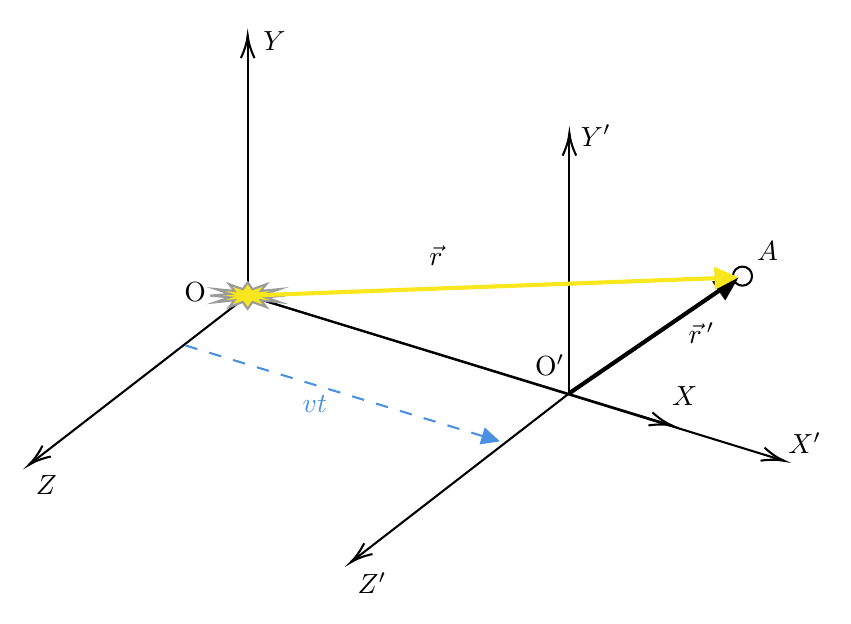
\begin{tikzpicture}[x=0.75pt,y=0.75pt,yscale=-1,xscale=1]
			%uncomment if require: \path (0,825); %set diagram left start at 0, and has height of 825
			
			%Straight Lines [id:da15000187622617145] 
			\draw    (236,181) -- (236,57.6) ;
			\draw [shift={(236,55.6)}, rotate = 90] [color={rgb, 255:red, 0; green, 0; blue, 0 }  ][line width=0.75]    (10.93,-3.29) .. controls (6.95,-1.4) and (3.31,-0.3) .. (0,0) .. controls (3.31,0.3) and (6.95,1.4) .. (10.93,3.29)   ;
			%Straight Lines [id:da7391133173163476] 
			\draw    (391,228) -- (391,104.6) ;
			\draw [shift={(391,102.6)}, rotate = 90] [color={rgb, 255:red, 0; green, 0; blue, 0 }  ][line width=0.75]    (10.93,-3.29) .. controls (6.95,-1.4) and (3.31,-0.3) .. (0,0) .. controls (3.31,0.3) and (6.95,1.4) .. (10.93,3.29)   ;
			%Straight Lines [id:da35796515703202303] 
			\draw    (236,181) -- (492.59,260.01) ;
			\draw [shift={(494.5,260.6)}, rotate = 197.12] [color={rgb, 255:red, 0; green, 0; blue, 0 }  ][line width=0.75]    (10.93,-3.29) .. controls (6.95,-1.4) and (3.31,-0.3) .. (0,0) .. controls (3.31,0.3) and (6.95,1.4) .. (10.93,3.29)   ;
			%Straight Lines [id:da6662748177038846] 
			\draw    (236,181) -- (438.59,243.01) ;
			\draw [shift={(440.5,243.6)}, rotate = 197.02] [color={rgb, 255:red, 0; green, 0; blue, 0 }  ][line width=0.75]    (10.93,-3.29) .. controls (6.95,-1.4) and (3.31,-0.3) .. (0,0) .. controls (3.31,0.3) and (6.95,1.4) .. (10.93,3.29)   ;
			%Straight Lines [id:da41386254054045435] 
			\draw    (236,181) -- (132.08,261.38) ;
			\draw [shift={(130.5,262.6)}, rotate = 322.28] [color={rgb, 255:red, 0; green, 0; blue, 0 }  ][line width=0.75]    (10.93,-3.29) .. controls (6.95,-1.4) and (3.31,-0.3) .. (0,0) .. controls (3.31,0.3) and (6.95,1.4) .. (10.93,3.29)   ;
			%Straight Lines [id:da7881076801433373] 
			\draw    (391,228) -- (287.08,308.38) ;
			\draw [shift={(285.5,309.6)}, rotate = 322.28] [color={rgb, 255:red, 0; green, 0; blue, 0 }  ][line width=0.75]    (10.93,-3.29) .. controls (6.95,-1.4) and (3.31,-0.3) .. (0,0) .. controls (3.31,0.3) and (6.95,1.4) .. (10.93,3.29)   ;
			%Straight Lines [id:da3883244787142972] 
			\draw [color={rgb, 255:red, 74; green, 144; blue, 226 }  ,draw opacity=1 ] [dash pattern={on 4.5pt off 4.5pt}]  (206,205) -- (326.35,241.7) -- (354.63,250.32) ;
			\draw [shift={(357.5,251.2)}, rotate = 196.96] [fill={rgb, 255:red, 74; green, 144; blue, 226 }  ,fill opacity=1 ][line width=0.08]  [draw opacity=0] (8.93,-4.29) -- (0,0) -- (8.93,4.29) -- cycle    ;
			%Straight Lines [id:da3425508680903211] 
			\draw [color={rgb, 255:red, 0; green, 0; blue, 0 }  ,draw opacity=1 ][line width=1.5]    (391,228) -- (469.2,174.46) ;
			\draw [shift={(472.5,172.2)}, rotate = 145.6] [fill={rgb, 255:red, 0; green, 0; blue, 0 }  ,fill opacity=1 ][line width=0.08]  [draw opacity=0] (11.61,-5.58) -- (0,0) -- (11.61,5.58) -- cycle    ;
			%Shape: Circle [id:dp5534520562104084] 
			\draw   (469.8,171.6) .. controls (469.8,169.06) and (471.86,167) .. (474.4,167) .. controls (476.94,167) and (479,169.06) .. (479,171.6) .. controls (479,174.14) and (476.94,176.2) .. (474.4,176.2) .. controls (471.86,176.2) and (469.8,174.14) .. (469.8,171.6) -- cycle ;
			%Shape: Star [id:dp08776025241886987] 
			\draw  [color={rgb, 255:red, 155; green, 155; blue, 155 }  ,draw opacity=1 ][fill={rgb, 255:red, 248; green, 231; blue, 28 }  ,fill opacity=1 ] (236,174.6) -- (238.33,177.91) -- (245,175.46) -- (242.36,178.74) -- (251.59,177.8) -- (244.69,180.17) -- (254,181) -- (244.69,181.83) -- (251.59,184.2) -- (242.36,183.26) -- (245,186.54) -- (238.33,184.09) -- (236,187.4) -- (233.67,184.09) -- (227,186.54) -- (229.64,183.26) -- (220.41,184.2) -- (227.31,181.83) -- (218,181) -- (227.31,180.17) -- (220.41,177.8) -- (229.64,178.74) -- (227,175.46) -- (233.67,177.91) -- cycle ;
			%Straight Lines [id:da0461746867695636] 
			\draw [color={rgb, 255:red, 248; green, 231; blue, 28 }  ,draw opacity=1 ][line width=1.5]    (236,181) -- (468.5,172.35) ;
			\draw [shift={(472.5,172.2)}, rotate = 177.87] [fill={rgb, 255:red, 248; green, 231; blue, 28 }  ,fill opacity=1 ][line width=0.08]  [draw opacity=0] (11.61,-5.58) -- (0,0) -- (11.61,5.58) -- cycle    ;
			
			% Text Node
			\draw (204,173) node [anchor=north west][inner sep=0.75pt]   [align=left] {O};
			% Text Node
			\draw (373,208) node [anchor=north west][inner sep=0.75pt]   [align=left] {O$'$};
			% Text Node
			\draw (242,52.4) node [anchor=north west][inner sep=0.75pt]    {$Y$};
			% Text Node
			\draw (395,97.4) node [anchor=north west][inner sep=0.75pt]    {$Y'$};
			% Text Node
			\draw (439,223.4) node [anchor=north west][inner sep=0.75pt]    {$X$};
			% Text Node
			\draw (495,245.4) node [anchor=north west][inner sep=0.75pt]    {$X'$};
			% Text Node
			\draw (132.5,266) node [anchor=north west][inner sep=0.75pt]    {$Z$};
			% Text Node
			\draw (287.5,313) node [anchor=north west][inner sep=0.75pt]    {$Z'$};
			% Text Node
			\draw (261,227.4) node [anchor=north west][inner sep=0.75pt]  [color={rgb, 255:red, 74; green, 144; blue, 226 }  ,opacity=1 ]  {$vt$};
			% Text Node
			\draw (322,155.4) node [anchor=north west][inner sep=0.75pt]    {$\vec{r}$};
			% Text Node
			\draw (447,192.4) node [anchor=north west][inner sep=0.75pt]    {$\vec{r} \,'$};
			% Text Node
			\draw (480,153.4) node [anchor=north west][inner sep=0.75pt]    {$A$};
			
			\end{tikzpicture}
	\end{figure}
	Its length is then the distance between its both ends:
	
	For the observer O, the object is moving. The positions $A$ and $B$ should therefore be measured simultaneously:
	
	So it comes using the relation proved earlier in this section:
	
	the following difference:
	
	hence the remarkable result:
	
	we also find the relation frequently in the literature as follows:
	
	Thus, the length of an observed rule in a moving frame relatively to the proper frame of the rule is less than its own length (which can assimilate in generality to a "\NewTerm{proper length}\index{proper length}"). In other words, the length of a moving object measured by the fixed reference frame will be measured shorter than its real proper size. This phenomenon is named "\NewTerm{length contraction}\index{length contraction}".
	\begin{figure}[H]
		\centering
		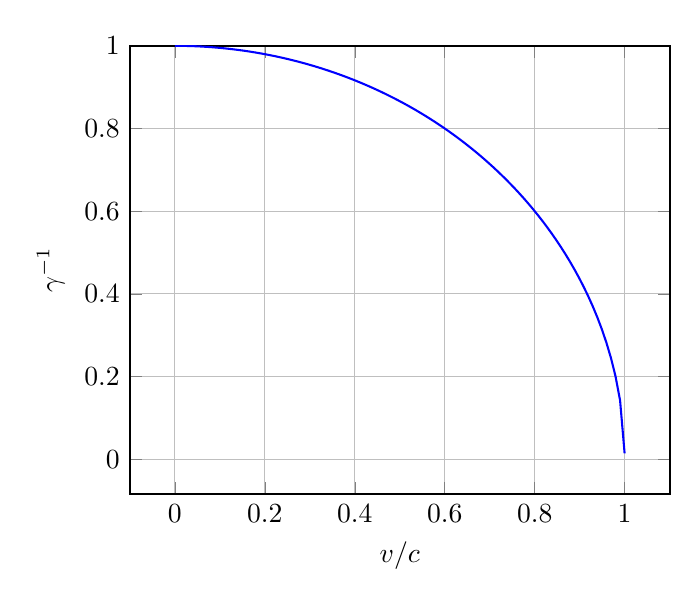
\begin{tikzpicture}[scale=1,declare function={Lorentz(\x,\c)=sqrt(1-(\x/\c)*(\x/\c));}]
		\begin{axis}[ymax=1,ylabel={$\gamma^{-1}$},xlabel={$v/c$},grid = major]
		 \addplot[blue,domain=0:1,samples=100] {Lorentz(x,1)};
		\end{axis}
		\end{tikzpicture}
		\caption{Lorentz factor length contraction function trend}
	\end{figure} 
	\begin{figure}[H]
		\centering
		\includegraphics[scale=0.95]{img/cosmology/start_trek.jpg} 
		\vspace*{2mm}	
		\caption[Length contraction principle for rectilinear motion]{Length contraction principle for rectilinear motion (source:?)}
	\end{figure}
	Due to superficial application of the contraction formula some paradoxes can occur. Examples are the "ladder paradox" and "Bell's spaceship paradox". However, those paradoxes can simply be solved by a correct application of relativity of simultaneity. Another famous paradox is the "Ehrenfest paradox" (high relativistic speed "rigid" rotating disc\footnote{Circumference of a rotating disk should contract but not the radius, as radius is perpendicular to the direction of motion.}), which proves that the concept of rigid bodies is not compatible with relativity, reducing the applicability of Born rigidity, and showing that for a co-rotating observer the geometry is in fact non-euclidean and we need then to use General Relativity.
	
	\begin{tcolorbox}[enhanced,colback=red!5!white,colframe=black!50!red,boxrule=1pt,arc=0pt,outer arc=0pt,drop lifted shadow,after skip=10pt plus 2pt]
	\bcbombe Caution! As we already have proved it earlier, length contraction, when expressed in the formalism of matrix algebra, is in fact a rotation in space-time (a hyperbolic rotation!!!)! So physically an object isn't smaller when moving, but is just seen with a different angle (i.e. in a different perspective angle) than the perpendicular one by default (at $v=0$) in space-time, and hence it looks smaller (however length contraction isn't also a visual effect as may make think the last sentence!).
	\end{tcolorbox}
	
	\subsubsection{Relativistic apparent angle rotation (Lampa–Terrell–Penrose effect)}
	The reader may have noticed something. The result of length contraction we have derived above for an imaginary one dimensional line is equivalent as if the line was rotated as illustrated below by an angle $\theta$:
	\begin{figure}[H]
		\centering			
		\begin{tikzpicture}[x=0.75pt,y=0.75pt,yscale=-1,xscale=1]
		%uncomment if require: \path (0,972); %set diagram left start at 0, and has height of 972
		
		% Pattern Info
		 
		\tikzset{
		pattern size/.store in=\mcSize, 
		pattern size = 5pt,
		pattern thickness/.store in=\mcThickness, 
		pattern thickness = 0.3pt,
		pattern radius/.store in=\mcRadius, 
		pattern radius = 1pt}
		\makeatletter
		\pgfutil@ifundefined{pgf@pattern@name@_m7lz2e2qo}{
		\pgfdeclarepatternformonly[\mcThickness,\mcSize]{_m7lz2e2qo}
		{\pgfqpoint{-\mcThickness}{-\mcThickness}}
		{\pgfpoint{\mcSize}{\mcSize}}
		{\pgfpoint{\mcSize}{\mcSize}}
		{
		\pgfsetcolor{\tikz@pattern@color}
		\pgfsetlinewidth{\mcThickness}
		\pgfpathmoveto{\pgfpointorigin}
		\pgfpathlineto{\pgfpoint{0}{\mcSize}}
		\pgfusepath{stroke}
		}}
		
		% Pattern Info
		\tikzset{
		pattern size/.store in=\mcSize, 
		pattern size = 5pt,
		pattern thickness/.store in=\mcThickness, 
		pattern thickness = 0.3pt,
		pattern radius/.store in=\mcRadius, 
		pattern radius = 1pt}
		\makeatletter
		\pgfutil@ifundefined{pgf@pattern@name@_whlp5dc81}{
		\pgfdeclarepatternformonly[\mcThickness,\mcSize]{_whlp5dc81}
		{\pgfqpoint{-\mcThickness}{-\mcThickness}}
		{\pgfpoint{\mcSize}{\mcSize}}
		{\pgfpoint{\mcSize}{\mcSize}}
		{
		\pgfsetcolor{\tikz@pattern@color}
		\pgfsetlinewidth{\mcThickness}
		\pgfpathmoveto{\pgfpointorigin}
		\pgfpathlineto{\pgfpoint{0}{\mcSize}}
		\pgfusepath{stroke}
		}}
		
		% Pattern Info
		\tikzset{
		pattern size/.store in=\mcSize, 
		pattern size = 5pt,
		pattern thickness/.store in=\mcThickness, 
		pattern thickness = 0.3pt,
		pattern radius/.store in=\mcRadius, 
		pattern radius = 1pt}
		\makeatletter
		\pgfutil@ifundefined{pgf@pattern@name@_doxk5kdqv}{
		\pgfdeclarepatternformonly[\mcThickness,\mcSize]{_doxk5kdqv}
		{\pgfqpoint{-\mcThickness}{-\mcThickness}}
		{\pgfpoint{\mcSize}{\mcSize}}
		{\pgfpoint{\mcSize}{\mcSize}}
		{
		\pgfsetcolor{\tikz@pattern@color}
		\pgfsetlinewidth{\mcThickness}
		\pgfpathmoveto{\pgfpointorigin}
		\pgfpathlineto{\pgfpoint{0}{\mcSize}}
		\pgfusepath{stroke}
		}}
		
		% Pattern Info
		\tikzset{
		pattern size/.store in=\mcSize, 
		pattern size = 5pt,
		pattern thickness/.store in=\mcThickness, 
		pattern thickness = 0.3pt,
		pattern radius/.store in=\mcRadius, 
		pattern radius = 1pt}
		\makeatletter
		\pgfutil@ifundefined{pgf@pattern@name@_39t84eep1}{
		\pgfdeclarepatternformonly[\mcThickness,\mcSize]{_39t84eep1}
		{\pgfqpoint{-\mcThickness}{-\mcThickness}}
		{\pgfpoint{\mcSize}{\mcSize}}
		{\pgfpoint{\mcSize}{\mcSize}}
		{
		\pgfsetcolor{\tikz@pattern@color}
		\pgfsetlinewidth{\mcThickness}
		\pgfpathmoveto{\pgfpointorigin}
		\pgfpathlineto{\pgfpoint{0}{\mcSize}}
		\pgfusepath{stroke}
		}}
		
		%Shape: Rectangle [id:dp5485836665370425] 
		\draw  [color={rgb, 255:red, 216; green, 216; blue, 216 }  ,draw opacity=1 ][pattern=_m7lz2e2qo,pattern size=6pt,pattern thickness=0.75pt,pattern radius=0pt, pattern color={rgb, 255:red, 211; green, 211; blue, 211}] (438,147) -- (540.5,147) -- (540.5,159) -- (438,159) -- cycle ;
		%Shape: Axis 2D [id:dp3920741742004661] 
		\draw  (63,213) -- (286.5,213)(85.35,42) -- (85.35,232) (279.5,208) -- (286.5,213) -- (279.5,218) (80.35,49) -- (85.35,42) -- (90.35,49)  ;
		%Shape: Rectangle [id:dp6707029838852474] 
		\draw  [pattern=_whlp5dc81,pattern size=6pt,pattern thickness=0.75pt,pattern radius=0pt, pattern color={rgb, 255:red, 0; green, 0; blue, 0}] (136,148) -- (238.5,148) -- (238.5,160) -- (136,160) -- cycle ;
		%Shape: Pie [id:dp1524728652997287] 
		\draw  [fill={rgb, 255:red, 0; green, 0; blue, 0 }  ,fill opacity=1 ] (168.06,261.13) .. controls (173.53,254.28) and (181.34,250) .. (190,250) .. controls (198.09,250) and (205.43,253.74) .. (210.83,259.81) -- (190,285) -- cycle ;
		%Straight Lines [id:da4920280805993624] 
		\draw    (155.5,248) -- (190,285) ;
		%Straight Lines [id:da8433733803690109] 
		\draw    (190,285) -- (222.5,249) ;
		%Right Arrow [id:dp7846582804088409] 
		\draw   (304,118) -- (325.3,118) -- (325.3,108) -- (339.5,128) -- (325.3,148) -- (325.3,138) -- (304,138) -- cycle ;
		%Shape: Axis 2D [id:dp11043579584070407] 
		\draw  (360,213) -- (583.5,213)(382.35,42) -- (382.35,232) (576.5,208) -- (583.5,213) -- (576.5,218) (377.35,49) -- (382.35,42) -- (387.35,49)  ;
		%Shape: Rectangle [id:dp9758238203860514] 
		\draw  [pattern=_doxk5kdqv,pattern size=5.550000000000001pt,pattern thickness=0.75pt,pattern radius=0pt, pattern color={rgb, 255:red, 0; green, 0; blue, 0}] (438,147) -- (516.5,147) -- (516.5,159) -- (438,159) -- cycle ;
		%Shape: Pie [id:dp38910717055642685] 
		\draw  [fill={rgb, 255:red, 0; green, 0; blue, 0 }  ,fill opacity=1 ] (465.06,261.13) .. controls (470.53,254.28) and (478.34,250) .. (487,250) .. controls (495.09,250) and (502.43,253.74) .. (507.83,259.81) -- (487,285) -- cycle ;
		%Straight Lines [id:da5677607110912473] 
		\draw    (452.5,248) -- (487,285) ;
		%Straight Lines [id:da39098424782367713] 
		\draw    (487,285) -- (519.5,249) ;
		%Shape: Rectangle [id:dp8831288671534911] 
		\draw  [color={rgb, 255:red, 216; green, 216; blue, 216 }  ,draw opacity=1 ][pattern=_39t84eep1,pattern size=6pt,pattern thickness=0.75pt,pattern radius=0pt, pattern color={rgb, 255:red, 211; green, 211; blue, 211}] (430.38,149.73) -- (509.59,84.67) -- (517.21,93.94) -- (438,159) -- cycle ;
		%Shape: Arc [id:dp3573320705274685] 
		\draw  [draw opacity=0] (476.32,128.48) .. controls (484.65,131.2) and (491.38,137.47) .. (494.72,145.5) -- (467,157) -- cycle ; \draw   (476.32,128.48) .. controls (484.65,131.2) and (491.38,137.47) .. (494.72,145.5) ;  
		%Straight Lines [id:da5545177816271196] 
		\draw  [dash pattern={on 4.5pt off 4.5pt}]  (516.5,147) -- (516.5,93.94) ;
		
		% Text Node
		\draw (290,209.4) node [anchor=north west][inner sep=0.75pt]    {$x$};
		% Text Node
		\draw (64,31.4) node [anchor=north west][inner sep=0.75pt]    {$y$};
		% Text Node
		\draw (160,295) node [anchor=north west][inner sep=0.75pt]   [align=left] {observer};
		% Text Node
		\draw (137,186) node [anchor=north west][inner sep=0.75pt]   [align=left] {at rest $\displaystyle v=0$};
		% Text Node
		\draw (587,209.4) node [anchor=north west][inner sep=0.75pt]    {$x$};
		% Text Node
		\draw (361,31.4) node [anchor=north west][inner sep=0.75pt]    {$y$};
		% Text Node
		\draw (457,295) node [anchor=north west][inner sep=0.75pt]   [align=left] {observer};
		% Text Node
		\draw (413,184) node [anchor=north west][inner sep=0.75pt]   [align=left] {in movement $\displaystyle v\gg 0$};
		% Text Node
		\draw (180,126.4) node [anchor=north west][inner sep=0.75pt]    {$L'$};
		% Text Node
		\draw (544,144.4) node [anchor=north west][inner sep=0.75pt]  [color={rgb, 255:red, 155; green, 155; blue, 155 }  ,opacity=1 ]  {$L'$};
		% Text Node
		\draw (466,84.4) node [anchor=north west][inner sep=0.75pt]  [color={rgb, 255:red, 155; green, 155; blue, 155 }  ,opacity=1 ]  {$L'$};
		% Text Node
		\draw (474,162.4) node [anchor=north west][inner sep=0.75pt]    {$L$};
		% Text Node
		\draw (491,120.4) node [anchor=north west][inner sep=0.75pt]    {$\theta $};
		\end{tikzpicture}
	\end{figure}
	We have immediately:
	
	Hence:
	
	We can find the above relation written differently using the trigonometric identity:
	
	Therefore:
	
	Hence:
	
	Finally:
	
	So the above relation can be written as the "\NewTerm{relativistic apparent angle rotation}\index{relativistic apparent angle rotation}":
	
	If we assume the equivalence that a contraction is equivalent to a rotation! That means we should be able to see the left side of the rode (or stick) - that is not visible when the speed is zero - and therefore the total length observed is not only that of given by $L$ (contracted length) but also we have to add to it a fraction of the thickness of the rode (or stick)! That also means that the illustration above with the Spaceship is inaccurate! We should be able to see the side of the ship as it approach the speed of light!
	
	In the case of a cube of side $L'$ we can illustrate the situation as following:
	\begin{figure}[H]
		\centering
		\begin{tikzpicture}[x=0.75pt,y=0.75pt,yscale=-1,xscale=1]
		%uncomment if require: \path (0,972); %set diagram left start at 0, and has height of 972
		
		%Shape: Axis 2D [id:dp11043579584070407] 
		\draw  (182,223) -- (405.5,223)(204.35,52) -- (204.35,242) (398.5,218) -- (405.5,223) -- (398.5,228) (199.35,59) -- (204.35,52) -- (209.35,59)  ;
		%Shape: Pie [id:dp38910717055642685] 
		\draw  [fill={rgb, 255:red, 0; green, 0; blue, 0 }  ,fill opacity=1 ] (287.06,271.13) .. controls (292.53,264.28) and (300.34,260) .. (309,260) .. controls (317.09,260) and (324.43,263.74) .. (329.83,269.81) -- (309,295) -- cycle ;
		%Straight Lines [id:da5677607110912473] 
		\draw    (274.5,258) -- (309,295) ;
		%Straight Lines [id:da39098424782367713] 
		\draw    (309,295) -- (341.5,259) ;
		%Shape: Square [id:dp9116976158160297] 
		\draw  [color={rgb, 255:red, 155; green, 155; blue, 155 }  ,draw opacity=1 ][line width=1.5]  (283.35,85.17) -- (367.83,51.35) -- (401.65,135.83) -- (317.17,169.65) -- cycle ;
		%Shape: Square [id:dp4590905152447502] 
		\draw  [color={rgb, 255:red, 0; green, 0; blue, 0 }  ,draw opacity=1 ][line width=1.5]  (316.69,98.38) -- (387.49,98.38) -- (387.49,169.18) -- (316.69,169.18) -- cycle ;
		%Shape: Arc [id:dp6955773459385315] 
		\draw  [draw opacity=0] (397.21,138.49) .. controls (400.98,148.15) and (403.04,158.66) .. (403.04,169.65) .. controls (403.04,169.77) and (403.04,169.89) .. (403.04,170.01) -- (317.17,169.65) -- cycle ; \draw  [color={rgb, 255:red, 155; green, 155; blue, 155 }  ,draw opacity=1 ] (397.21,138.49) .. controls (400.98,148.15) and (403.04,158.66) .. (403.04,169.65) .. controls (403.04,169.77) and (403.04,169.89) .. (403.04,170.01) ;  
		%Straight Lines [id:da10714871853090768] 
		\draw  [dash pattern={on 4.5pt off 4.5pt}]  (283.35,85.17) -- (283.35,169) ;
		%Straight Lines [id:da08255039363369487] 
		\draw  [dash pattern={on 4.5pt off 4.5pt}]  (315.02,169) -- (285.35,169) ;
		\draw [shift={(283.35,169)}, rotate = 360] [color={rgb, 255:red, 0; green, 0; blue, 0 }  ][line width=0.75]    (10.93,-3.29) .. controls (6.95,-1.4) and (3.31,-0.3) .. (0,0) .. controls (3.31,0.3) and (6.95,1.4) .. (10.93,3.29)   ;
		\draw [shift={(317.02,169)}, rotate = 180] [color={rgb, 255:red, 0; green, 0; blue, 0 }  ][line width=0.75]    (10.93,-3.29) .. controls (6.95,-1.4) and (3.31,-0.3) .. (0,0) .. controls (3.31,0.3) and (6.95,1.4) .. (10.93,3.29)   ;
		%Shape: Arc [id:dp7034398202741055] 
		\draw  [draw opacity=0] (264.74,170.01) .. controls (264.74,169.89) and (264.74,169.77) .. (264.74,169.65) .. controls (264.74,147.27) and (278.76,128.16) .. (298.5,120.64) -- (317.17,169.65) -- cycle ; \draw  [color={rgb, 255:red, 155; green, 155; blue, 155 }  ,draw opacity=1 ] (264.74,170.01) .. controls (264.74,169.89) and (264.74,169.77) .. (264.74,169.65) .. controls (264.74,147.27) and (278.76,128.16) .. (298.5,120.64) ;  
		
		% Text Node
		\draw (409,219.4) node [anchor=north west][inner sep=0.75pt]    {$x$};
		% Text Node
		\draw (183,41.4) node [anchor=north west][inner sep=0.75pt]    {$y$};
		% Text Node
		\draw (279,305) node [anchor=north west][inner sep=0.75pt]   [align=left] {observer};
		% Text Node
		\draw (271,194) node [anchor=north west][inner sep=0.75pt]   [align=left] {in movement $\displaystyle v\gg 0$};
		% Text Node
		\draw (389,75.4) node [anchor=north west][inner sep=0.75pt]  [color={rgb, 255:red, 155; green, 155; blue, 155 }  ,opacity=1 ]  {$L'$};
		% Text Node
		\draw (344,172.9) node [anchor=north west][inner sep=0.75pt]    {$L$};
		% Text Node
		\draw (300,110.4) node [anchor=north west][inner sep=0.75pt]  [color={rgb, 255:red, 155; green, 155; blue, 155 }  ,opacity=1 ]  {$L'$};
		% Text Node
		\draw (315,47.4) node [anchor=north west][inner sep=0.75pt]  [color={rgb, 255:red, 155; green, 155; blue, 155 }  ,opacity=1 ]  {$L'$};
		% Text Node
		\draw (348,132.4) node [anchor=north west][inner sep=0.75pt]  [color={rgb, 255:red, 155; green, 155; blue, 155 }  ,opacity=1 ]  {$L'$};
		% Text Node
		\draw (292.35,172.4) node [anchor=north west][inner sep=0.75pt]    {$L''$};
		% Text Node
		\draw (403,146.4) node [anchor=north west][inner sep=0.75pt]  [color={rgb, 255:red, 155; green, 155; blue, 155 }  ,opacity=1 ]  {$\theta $};
		% Text Node
		\draw (220,122.4) node [anchor=north west][inner sep=0.75pt]  [color={rgb, 255:red, 155; green, 155; blue, 155 }  ,opacity=1 ]  {$\dfrac{\pi }{2} -\theta $};
		\end{tikzpicture}
	\end{figure}
	We have from the figure above:
	
	Hence using trigonometric identities:
	
	Therefore rearranging and using previous result:
	
	Hence the total length seen by the observer:
	
	The "\NewTerm{Terrell rotation}\index{Terrell rotation}" or "\NewTerm{Terrell effect}\index{Terrell effect}" is the visual distortion that a passing object would appear to undergo, according to the special theory of relativity if it were travelling at a significant fraction of the speed of light. This behaviour was described independently by both Roger Penrose and James Terrell. Penrose's article was submitted 29 July 11958 (holocene calendar) and published in January 11959 (holocene calendar). Terrell's article was submitted 22 June 11959 (holocene calendar) and published 15 November 11959 (holocene calendar). The general phenomenon was noted already in 11924 (holocene calendar) by Austrian physicist Anton Lampa. 
	
	Due to a dispute about priority and correct attribution, the effect is also sometimes referred to as the "Penrose–Terrell effect", the "Terrell–Penrose effect" or the "Lampa–Terrell–Penrose effect", but not the "Lampa effect".
	
	\subsubsection{Relativistic time variation (time dilatation)}\label{relativistic time variation}
	An event is a phenomenon that occurs in a given place at a given time. The origin of time is difficult to determine, we often prefer to define the concept of "time interval" as the time elapsed between two events as it is often customary (\SeeChapter{see section Principia page \pageref{time}}).
	
	Let us now consider two consecutive events $A$ and $B$ that occur at the same location $x'$ (!) in the repository in uniform translation:
	\begin{figure}[H]
		\centering
		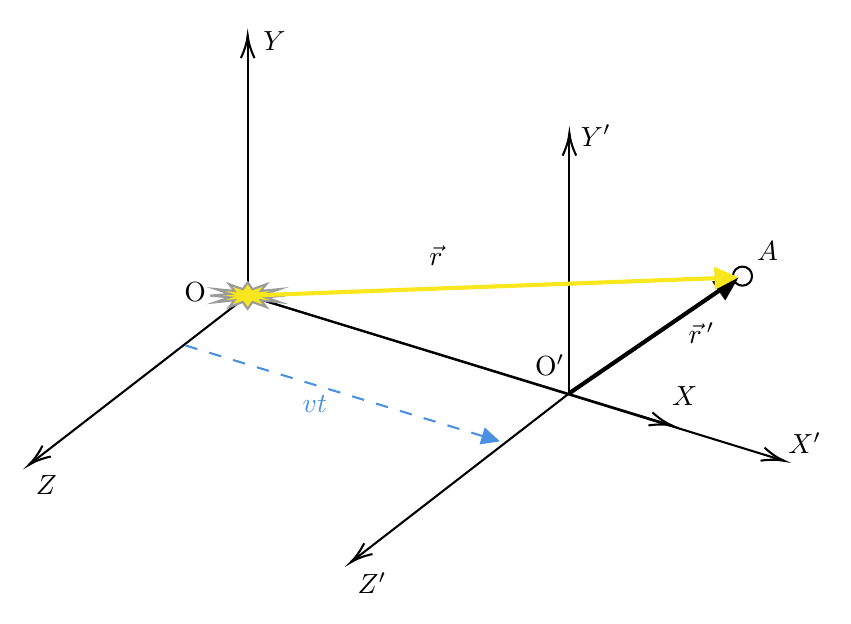
\begin{tikzpicture}[x=0.75pt,y=0.75pt,yscale=-1,xscale=1]
		%uncomment if require: \path (0,825); %set diagram left start at 0, and has height of 825
		
		%Straight Lines [id:da15000187622617145] 
		\draw    (236,181) -- (236,57.6) ;
		\draw [shift={(236,55.6)}, rotate = 90] [color={rgb, 255:red, 0; green, 0; blue, 0 }  ][line width=0.75]    (10.93,-3.29) .. controls (6.95,-1.4) and (3.31,-0.3) .. (0,0) .. controls (3.31,0.3) and (6.95,1.4) .. (10.93,3.29)   ;
		%Straight Lines [id:da7391133173163476] 
		\draw    (391,228) -- (391,104.6) ;
		\draw [shift={(391,102.6)}, rotate = 90] [color={rgb, 255:red, 0; green, 0; blue, 0 }  ][line width=0.75]    (10.93,-3.29) .. controls (6.95,-1.4) and (3.31,-0.3) .. (0,0) .. controls (3.31,0.3) and (6.95,1.4) .. (10.93,3.29)   ;
		%Straight Lines [id:da35796515703202303] 
		\draw    (236,181) -- (492.59,260.01) ;
		\draw [shift={(494.5,260.6)}, rotate = 197.12] [color={rgb, 255:red, 0; green, 0; blue, 0 }  ][line width=0.75]    (10.93,-3.29) .. controls (6.95,-1.4) and (3.31,-0.3) .. (0,0) .. controls (3.31,0.3) and (6.95,1.4) .. (10.93,3.29)   ;
		%Straight Lines [id:da6662748177038846] 
		\draw    (236,181) -- (438.59,243.01) ;
		\draw [shift={(440.5,243.6)}, rotate = 197.02] [color={rgb, 255:red, 0; green, 0; blue, 0 }  ][line width=0.75]    (10.93,-3.29) .. controls (6.95,-1.4) and (3.31,-0.3) .. (0,0) .. controls (3.31,0.3) and (6.95,1.4) .. (10.93,3.29)   ;
		%Straight Lines [id:da41386254054045435] 
		\draw    (236,181) -- (132.08,261.38) ;
		\draw [shift={(130.5,262.6)}, rotate = 322.28] [color={rgb, 255:red, 0; green, 0; blue, 0 }  ][line width=0.75]    (10.93,-3.29) .. controls (6.95,-1.4) and (3.31,-0.3) .. (0,0) .. controls (3.31,0.3) and (6.95,1.4) .. (10.93,3.29)   ;
		%Straight Lines [id:da7881076801433373] 
		\draw    (391,228) -- (287.08,308.38) ;
		\draw [shift={(285.5,309.6)}, rotate = 322.28] [color={rgb, 255:red, 0; green, 0; blue, 0 }  ][line width=0.75]    (10.93,-3.29) .. controls (6.95,-1.4) and (3.31,-0.3) .. (0,0) .. controls (3.31,0.3) and (6.95,1.4) .. (10.93,3.29)   ;
		%Straight Lines [id:da3883244787142972] 
		\draw [color={rgb, 255:red, 74; green, 144; blue, 226 }  ,draw opacity=1 ] [dash pattern={on 4.5pt off 4.5pt}]  (206,205) -- (326.35,241.7) -- (354.63,250.32) ;
		\draw [shift={(357.5,251.2)}, rotate = 196.96] [fill={rgb, 255:red, 74; green, 144; blue, 226 }  ,fill opacity=1 ][line width=0.08]  [draw opacity=0] (8.93,-4.29) -- (0,0) -- (8.93,4.29) -- cycle    ;
		%Straight Lines [id:da3425508680903211] 
		\draw [color={rgb, 255:red, 0; green, 0; blue, 0 }  ,draw opacity=1 ][line width=1.5]    (391,228) -- (469.2,174.46) ;
		\draw [shift={(472.5,172.2)}, rotate = 145.6] [fill={rgb, 255:red, 0; green, 0; blue, 0 }  ,fill opacity=1 ][line width=0.08]  [draw opacity=0] (11.61,-5.58) -- (0,0) -- (11.61,5.58) -- cycle    ;
		%Shape: Circle [id:dp5534520562104084] 
		\draw   (469.8,171.6) .. controls (469.8,169.06) and (471.86,167) .. (474.4,167) .. controls (476.94,167) and (479,169.06) .. (479,171.6) .. controls (479,174.14) and (476.94,176.2) .. (474.4,176.2) .. controls (471.86,176.2) and (469.8,174.14) .. (469.8,171.6) -- cycle ;
		%Shape: Star [id:dp08776025241886987] 
		\draw  [color={rgb, 255:red, 155; green, 155; blue, 155 }  ,draw opacity=1 ][fill={rgb, 255:red, 248; green, 231; blue, 28 }  ,fill opacity=1 ] (236,174.6) -- (238.33,177.91) -- (245,175.46) -- (242.36,178.74) -- (251.59,177.8) -- (244.69,180.17) -- (254,181) -- (244.69,181.83) -- (251.59,184.2) -- (242.36,183.26) -- (245,186.54) -- (238.33,184.09) -- (236,187.4) -- (233.67,184.09) -- (227,186.54) -- (229.64,183.26) -- (220.41,184.2) -- (227.31,181.83) -- (218,181) -- (227.31,180.17) -- (220.41,177.8) -- (229.64,178.74) -- (227,175.46) -- (233.67,177.91) -- cycle ;
		%Straight Lines [id:da0461746867695636] 
		\draw [color={rgb, 255:red, 248; green, 231; blue, 28 }  ,draw opacity=1 ][line width=1.5]    (236,181) -- (468.5,172.35) ;
		\draw [shift={(472.5,172.2)}, rotate = 177.87] [fill={rgb, 255:red, 248; green, 231; blue, 28 }  ,fill opacity=1 ][line width=0.08]  [draw opacity=0] (11.61,-5.58) -- (0,0) -- (11.61,5.58) -- cycle    ;
		
		% Text Node
		\draw (204,173) node [anchor=north west][inner sep=0.75pt]   [align=left] {O};
		% Text Node
		\draw (373,208) node [anchor=north west][inner sep=0.75pt]   [align=left] {O$'$};
		% Text Node
		\draw (242,52.4) node [anchor=north west][inner sep=0.75pt]    {$Y$};
		% Text Node
		\draw (395,97.4) node [anchor=north west][inner sep=0.75pt]    {$Y'$};
		% Text Node
		\draw (439,223.4) node [anchor=north west][inner sep=0.75pt]    {$X$};
		% Text Node
		\draw (495,245.4) node [anchor=north west][inner sep=0.75pt]    {$X'$};
		% Text Node
		\draw (132.5,266) node [anchor=north west][inner sep=0.75pt]    {$Z$};
		% Text Node
		\draw (287.5,313) node [anchor=north west][inner sep=0.75pt]    {$Z'$};
		% Text Node
		\draw (261,227.4) node [anchor=north west][inner sep=0.75pt]  [color={rgb, 255:red, 74; green, 144; blue, 226 }  ,opacity=1 ]  {$vt$};
		% Text Node
		\draw (322,155.4) node [anchor=north west][inner sep=0.75pt]    {$\vec{r}$};
		% Text Node
		\draw (447,192.4) node [anchor=north west][inner sep=0.75pt]    {$\vec{r} \,'$};
		% Text Node
		\draw (480,153.4) node [anchor=north west][inner sep=0.75pt]    {$A$};
		
		\end{tikzpicture}
	\end{figure}
	For the observer in $\text{O}'$, the time interval is simply:
	
	To measure this time interval, the observer O in the fixed reference repository should also require that $x'$ is common to both events. Then using the relation proved earlier above:
	
	we get:
	
	hence the remarkable result:
	
	what we write under traditional condensed form:
	
	\begin{figure}[H]
		\centering
		\begin{minipage}{.5\textwidth}
		  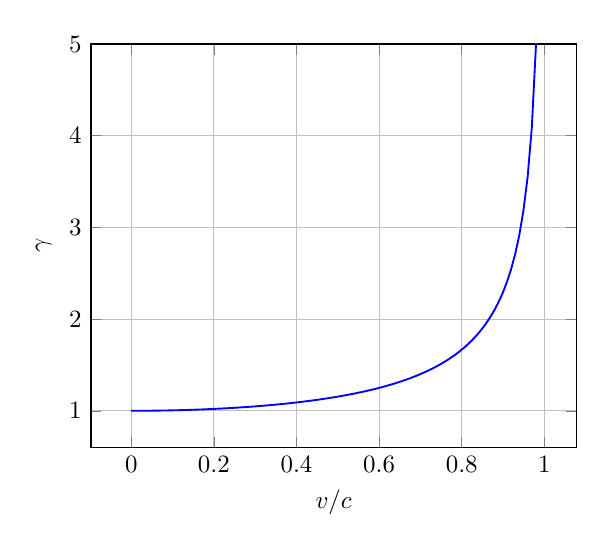
\begin{tikzpicture}[scale=0.90,declare function={Lorentz(\x,\c)=1/sqrt(1-(\x/\c)*(\x/\c));}]
		\begin{axis}[ymax=5,ylabel={$\gamma$},xlabel={$v/c$},grid = major]
		 \addplot[blue,domain=0:1,samples=100] {Lorentz(x,1)};
		\end{axis}
		\end{tikzpicture}
		\caption{Lorentz factor time dilatation function trend}
		\end{minipage}%
		\begin{minipage}{.5\textwidth}
		  \centering
		  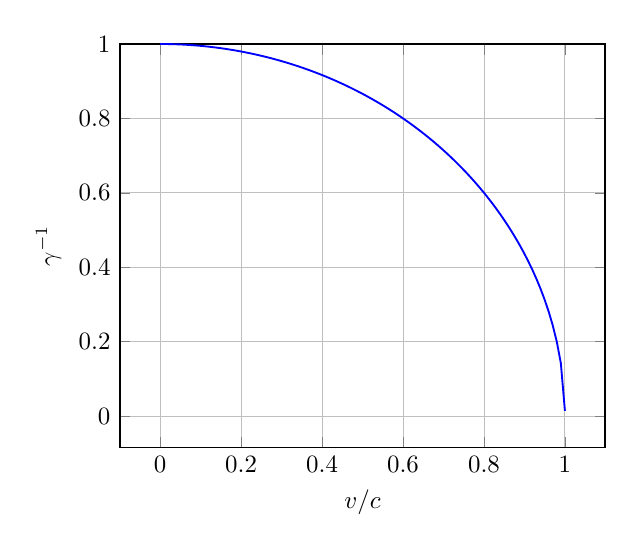
\begin{tikzpicture}[scale=0.90,declare function={Lorentz(\x,\c)=sqrt(1-(\x/\c)*(\x/\c));}]
		\begin{axis}[ymax=1,ylabel={$\gamma^{-1}$},xlabel={$v/c$},grid = major]
		 \addplot[blue,domain=0:1,samples=100] {Lorentz(x,1)};
		\end{axis}
		\end{tikzpicture}
		\caption[]{Lorentz length contraction function (reminder)}
		\end{minipage}
	\end{figure}
	
	We also deduce taking an infinitesimal time element:
	
	So the observer O (stationary) measures a time interval much larger than that one measured in the moving repository where the phenomenon takes place as it moves quickly. The time in the fixed repository (thus the "\NewTerm{proper time}\index{proper time}" of the fixed reference frame!) seems like dilated compared to that in occurring in the mobile reference frame (that is to say relatively to the "proper time" of mobile reference frame!).
	
	The conclusion is that there is no single universal time, rather there exist an infinite number of times, each specific to a different reference frame... therefore, defining any exact, unambiguous point in time is impossible (as far as we know today...)!
	
	\begin{tcolorbox}[enhanced,colback=red!5!white,colframe=black!50!red,boxrule=1pt,arc=0pt,outer arc=0pt,drop lifted shadow,after skip=10pt plus 2pt]
	\bcbombe Caution! A common error in Special Relativity is to think that time dilation is physical/real, ie the people moving will age more slowly. But that's wrong in Special Relativity (but not in General Relativity) and for exactly the same reasons as for the length dilatation (you just have to consider the axis of space $ct$ instead of the axis of pure time $t$).
	\end{tcolorbox}
	
	Let us see two applied examples\footnote{Apart from these two famous examples, time dilatation helps particle physicists at the LHC (CERN) to track some particles during high energy collisions that have a too short lifetime to be correctly observed and studied but that thanks to their high speed have a significant longer proper life time due to time dilatation! Therefore with time dilatation particle physicists have the opportunity to study some specific particles properties what would not be possible without! Hourrra!} that are so famous that they have their own name so that we will consider them as a table of contents entry for this book:
	
	\paragraph{Hafele–Keating experiment (special relativity version)}\label{hafele keating experiment special relativity}\mbox{}\\\\\
	In 11971 (holocene calendar), direct experimental verification of time dilation was performed. Two airplanes in whose had been placed a cesium atomic clock during their regular commercial flights (one flying to the east, the other to west) compared their clocks to a third  atomic clock remained on the ground. This experiment made famous by time is named today "\NewTerm{Hafele-Keating experiment}\index{Hafele-Keating experiment}" (Joseph C. Hafele, a physicist, and Richard E. Keating, an astronomer).
	\begin{figure}[H]
		\centering
		\includegraphics[scale=0.7]{img/cosmology/hafele_keating_experiment.jpg}
	\end{figure}
	Because the Hafele–Keating experiment has been reproduced by increasingly accurate methods, there has been a consensus among physicists since at least the 11970s (holocene calendar) that the relativistic predictions of gravitational and kinematic effects on time have been conclusively verified. Criticisms of the experiment did not address the subsequent verification of the result by more accurate methods, and have been shown to be in error.

	The idea is obviously that in a frame of reference at rest with respect to the center of the Earth, a clock aboard the plane moving eastward, in the direction of the Earth's rotation, has a greater velocity (resulting in a relative time loss) than one that remained on the ground, while a clock aboard the plane moving westward, against the Earth's rotation, had a lower velocity than one on the ground.
	
	The plane flying eastward lost $59$ [ns] while the plane flying westward gained $273$ [ns] (the Earth rotates on itself in a day, from West to East. It was therefore measured a total difference:
	
	between the two clocks and this difference is even statistically significantly greater than that the one implied by Special Relativity (see detailed calculations just below).

	Let us analyse the experience considering that all repositories are inertial (thus eliminating General Relativity).
	\begin{tcolorbox}[title=Remark,arc=10pt,breakable,drop lifted shadow,
  skin=enhanced,
  skin first is subskin of={enhancedfirst}{arc=10pt,no shadow},
  skin middle is subskin of={enhancedmiddle}{arc=10pt,no shadow},
  skin last is subskin of={enhancedlast}{drop lifted shadow}]
	Strictly speaking, the effect of General Relativity (slowing of clocks depending on the altitude in accordance with Einstein's effect proved in the section of General Relativity at page \pageref{gravitational redshift}) is absolutely not negligible since it is equivalent in amplitude that of Special Relativity. This is why we will study this experiment again in the section of General Relativity.
	\end{tcolorbox}
	Let us consider for our study  three inertial reference points, one at the North Pole, one on Earth (elsewhere apart from the North Pole in the idea!) and one in a plane. The time intervals $t_{\text{North}},t_{\text{Earth}}$ and $t_{\text{plane}}$ respectively (which we will abbreviated $t_N,t_E,t_P$ for the following developments), are connected by the previously proven relations (so the North pole is taken as the reference at rest in this experience and therefore the reference proper time!):
	
	where we have:
	
	The repository on Earth and in the plane so have equation relative speeds $v_E$ and $v_P$ relative to the North Pole. The time by plane and on Earth are then linked by:
	
	We will now rewrite this relation:
	
	We will accept the following approximation:
	
	where we have assumed that at the denominator:
	
	For square roots whose value is anyway close to $1$ (since $c$ is much larger than the considered relative speeds), we can do a Maclaurin expansion to the second order as $x$ approaches zero (\SeeChapter{see section Sequences and Series page \pageref{usual maclaurin developments}}):
	
	Then we can write:
	
	Thanks to these tricky successive approximations, we can easily write the difference between the two clocks that is then:
	
	According to the initial assumptions, the cruising speed of the two aircraft from the ground is constant and is denoted $v$. The speed of each plane (!non-relativistic according to the preceding approximations) is then:
	
	for the plane going eastwards and:
	
	for the aircraft going respectively westward. So:
	
	We will consider that (it's pretty rough ...):
	
	So it remains:
	
	We see well that obviously with the previous approximations we lost the asymmetry of time dilatation between East and West. The reader that this should disturb can then apply directly the numerical values in the prior previous relation.

	The previous result that we got with all successive approximations already leaded us to see formally and quickly that the sign of the result will be in agreement with experimental results.

	For a practical numerical application, we will take the constant speed of the commercial planes at that time that was:
	
	and the total time travel of planes was of $41$ hours according to the measurement at the ground, thus:
	
	and a point at the equator of the Earth's surface moves at the speed:
	
	where the Earth's radius being of $6,371$ [km] (this suppose that the plans are above the equator radius). We then have applying all that numerical values:
	
	which leads to a result very close to the measurement that was performed.

	And using directly the non-approximate version:
	
	where we took this time the speed of the Earth at latitude consistent with the experience in 11971 (holocene calendar):
	
	So we see that the result is therefore not very consistent with the experience! Indeed, we must now consider in that approximated case the time dilatation due to gravity. We'll have to use the Einstein's effect relation proved in the section of General Relativity (see page \pageref{gravitational redshift}) for approximated locally flat space:
	
	which expresses for recall the that at the ground time flows slower than the time at altitude $h$.
	
	According to the records of the experiment, the aircraft flew at $10,000$ [m] above sea level. What gives (the acceleration $g$ is not the same on the ground level than in altitude for recall!) and acceleration of time of:
	
	But, we see that the two aircraft were both at the same height, we always have:
	
	So either there are other effects, of the order of General Relativity, which should be taken into account to explain the $67$ [ns] of difference to the experience, or it is a accuracy problem of the time accuracy of the time clock at the time of the experiment.

	In fact, we will see a detailed study of this experience in the section of General Relativity and see that the theoretical values are in very good agreement with experimental results.
	
	\paragraph{Twins paradox}\mbox{}\\\\\
	The twin paradox is a thought experiment in Special Relativity involving identical twins, one of whom makes a journey into space in a high-speed rocket and returns home to find that the twin who remained on Earth has aged more. This result appears puzzling because each twin sees the other twin as moving, and so, according to an incorrect and naive application of time dilation and the principle of relativity, each should paradoxically find the other to have aged more slowly. However, this scenario can be resolved (again contrary to a popular misconception) within the standard framework of Special Relativity: the travelling twin's trajectory involves two different inertial frames, one for the outbound journey and one for the inbound journey, and so there is no symmetry between the space-time paths of the two twins. Therefore, the twin paradox is not a paradox in the sense of a logical contradiction.
	\begin{figure}[H]
		\centering
		\includegraphics[scale=0.5]{img/cosmology/twin_paradox.jpg}
	\end{figure}
	We can already consider the famous twin paradox in the framework of Special Relativity to show that the twin paradox does not only apply to non inertial systems. This is a rough approach (knowing that we will rigorously discussed the subject in the section of General Relativity).

	Let us consider a rocket taking off at time $t$ zero of the Earth and accelerating to $20$ times the acceleration of Earth's gravity $g$ up to a cruising speed of $90\%$ the speed of light $c$. Let us suppose that the rocket continues at this speed during a terrestrial year and decelerate with the same intensity to resume its journey to Earth and accelerates again for its approach to the Earth and decelerate once again to its final zero velocity:	
	
	Thus, the total proper time spent for a human remained on Earth is:
	
	For the traveller in the rocket, the proper time during the acceleration phase will be given roughly by:
	
	Thus by integrating (using the usual primitive proved in the section of Differential and Integral Calculus page \pageref{usual primitives}) for one of the phase of acceleration of the rocket it gives:
	
	And the proper time for the part with the constant cruising speed:
	
	And therefore the total proper time in the rocket is:
	
	So compared to the person remained on Earth, the one that was in the rocket has aged about half !!! This is a paradox (rather a "sophism" in reality) because we can not accurately apply Special Relativity to non-inertial frames. Nevertheless, even with General Relativity, there is a time difference!
	
	\begin{tcolorbox}[enhanced,colback=red!5!white,colframe=black!50!red,boxrule=1pt,arc=0pt,outer arc=0pt,drop lifted shadow,after skip=10pt plus 2pt]
	\bcbombe Caution! But we haven't solved the Langevin's paradox here! Because in the framework of Special Relativity both observers can be switched independently. And that's the problem of making the calculations with Special Relativity: the acceleration is relative. That doesn't make sense in real life (even if it's possible on the paper) because in reality, one of the observer will feel an acceleration and deceleration when the other one won't. And that's what General Relativity can deal with: it makes acceleration absolute!
	\end{tcolorbox}
	
	\subsubsection{Apparent relativistic mass}
	First the reader must take careful (!!) The title is misleading by tradition! We will see why a little further below.

	Meanwhile, imagine a frontal collision between two identical objects $(1)$ and $(2)$ having in the repository $R_0$ equal but opposite speeds. We will assume that the collision is elastic, that is to say that the kinetic energy and momentum are conserved.

	Before the shock (collision), the components of objects speeds $(1)$ and $(2)$ are:
	
	as shown below:
	\begin{figure}[H]
		\centering
		\begin{tikzpicture}[x=0.75pt,y=0.75pt,yscale=-1,xscale=1]
			%uncomment if require: \path (0,592); %set diagram left start at 0, and has height of 592
			
			%Shape: Axis 2D [id:dp06570943233518767] 
			\draw  (168,202.2) -- (472.3,202.2)(319.3,62) -- (319.3,341.2) (465.3,197.2) -- (472.3,202.2) -- (465.3,207.2) (314.3,69) -- (319.3,62) -- (324.3,69)  ;
			%Straight Lines [id:da5127709830417204] 
			\draw [color={rgb, 255:red, 208; green, 2; blue, 27 }  ,draw opacity=1 ] [dash pattern={on 4.5pt off 4.5pt}]  (321.52,200.18) -- (420.3,110.2) ;
			\draw [shift={(319.3,202.2)}, rotate = 317.67] [fill={rgb, 255:red, 208; green, 2; blue, 27 }  ,fill opacity=1 ][line width=0.08]  [draw opacity=0] (8.93,-4.29) -- (0,0) -- (8.93,4.29) -- cycle    ;
			%Straight Lines [id:da556116035917877] 
			\draw [color={rgb, 255:red, 208; green, 2; blue, 27 }  ,draw opacity=1 ] [dash pattern={on 4.5pt off 4.5pt}]  (319.3,202.2) -- (207.65,114.06) ;
			\draw [shift={(205.3,112.2)}, rotate = 38.29] [fill={rgb, 255:red, 208; green, 2; blue, 27 }  ,fill opacity=1 ][line width=0.08]  [draw opacity=0] (8.93,-4.29) -- (0,0) -- (8.93,4.29) -- cycle    ;
			%Straight Lines [id:da1470769305599242] 
			\draw [color={rgb, 255:red, 65; green, 117; blue, 5 }  ,draw opacity=1 ] [dash pattern={on 4.5pt off 4.5pt}]  (319.3,202.2) -- (417.21,303.05) ;
			\draw [shift={(419.3,305.2)}, rotate = 225.85] [fill={rgb, 255:red, 65; green, 117; blue, 5 }  ,fill opacity=1 ][line width=0.08]  [draw opacity=0] (8.93,-4.29) -- (0,0) -- (8.93,4.29) -- cycle    ;
			%Straight Lines [id:da7797955529836631] 
			\draw [color={rgb, 255:red, 65; green, 117; blue, 5 }  ,draw opacity=1 ] [dash pattern={on 4.5pt off 4.5pt}]  (317.14,204.28) -- (216.3,301.2) ;
			\draw [shift={(319.3,202.2)}, rotate = 136.13] [fill={rgb, 255:red, 65; green, 117; blue, 5 }  ,fill opacity=1 ][line width=0.08]  [draw opacity=0] (8.93,-4.29) -- (0,0) -- (8.93,4.29) -- cycle    ;
			
			% Text Node
			\draw (473,202.4) node [anchor=north west][inner sep=0.75pt]    {$X$};
			% Text Node
			\draw (296,55.4) node [anchor=north west][inner sep=0.75pt]    {$Y$};
			% Text Node
			\draw (415.15,91.4) node [anchor=north west][inner sep=0.75pt]    {$2$};
			% Text Node
			\draw (200.15,91.4) node [anchor=north west][inner sep=0.75pt]    {$2'$};
			% Text Node
			\draw (201.65,306.6) node [anchor=north west][inner sep=0.75pt]    {$1$};
			% Text Node
			\draw (413.65,306.6) node [anchor=north west][inner sep=0.75pt]    {$1'$};
		\end{tikzpicture} 
		\vspace*{3mm}
		\caption{Configuration for the study of the apparent relativistic mass variation seen from $R_0$}
	\end{figure}
	After the collision, we have:
	
	We will now apply the following Lorentz transformation:
	\begin{itemize}
		\item We give ourselves another repository $R$ and assume that the repositories $R_0$ and $R$ are in uniform translation speed $u_1$ along the $x$-axis in the positive direction (that is to say in the same direction and at the same horizontal speed than the particle $(1)$).
		
		\item For our particle $(1)$ its trajectory became such is present not visible speed anymore along the $x$-axis.
	\end{itemize}
	Let's go! Let us place ourselves in repository $R$ that moves relative to $R_0$ with the speed $u_1$ following the $x$-axis, the components of the speeds in this repository are ten before the collision:
	
	and after the collision:
	
	\begin{figure}[H]
		\centering
		\begin{tikzpicture}[x=0.75pt,y=0.75pt,yscale=-1,xscale=1]
		%uncomment if require: \path (0,592); %set diagram left start at 0, and has height of 592
		
		%Shape: Axis 2D [id:dp06570943233518767] 
		\draw  (168,202.2) -- (472.3,202.2)(319.3,62) -- (319.3,341.2) (465.3,197.2) -- (472.3,202.2) -- (465.3,207.2) (314.3,69) -- (319.3,62) -- (324.3,69)  ;
		%Straight Lines [id:da5127709830417204] 
		\draw [color={rgb, 255:red, 208; green, 2; blue, 27 }  ,draw opacity=1 ] [dash pattern={on 4.5pt off 4.5pt}]  (321.52,200.18) -- (420.3,110.2) ;
		\draw [shift={(319.3,202.2)}, rotate = 317.67] [fill={rgb, 255:red, 208; green, 2; blue, 27 }  ,fill opacity=1 ][line width=0.08]  [draw opacity=0] (8.93,-4.29) -- (0,0) -- (8.93,4.29) -- cycle    ;
		%Straight Lines [id:da556116035917877] 
		\draw [color={rgb, 255:red, 208; green, 2; blue, 27 }  ,draw opacity=1 ] [dash pattern={on 4.5pt off 4.5pt}]  (319.3,202.2) -- (207.65,114.06) ;
		\draw [shift={(205.3,112.2)}, rotate = 38.29] [fill={rgb, 255:red, 208; green, 2; blue, 27 }  ,fill opacity=1 ][line width=0.08]  [draw opacity=0] (8.93,-4.29) -- (0,0) -- (8.93,4.29) -- cycle    ;
		%Straight Lines [id:da1470769305599242] 
		\draw [color={rgb, 255:red, 65; green, 117; blue, 5 }  ,draw opacity=1 ] [dash pattern={on 4.5pt off 4.5pt}]  (323.3,203.2) -- (323.3,303.2) ;
		\draw [shift={(323.3,306.2)}, rotate = 270] [fill={rgb, 255:red, 65; green, 117; blue, 5 }  ,fill opacity=1 ][line width=0.08]  [draw opacity=0] (8.93,-4.29) -- (0,0) -- (8.93,4.29) -- cycle    ;
		%Straight Lines [id:da7797955529836631] 
		\draw [color={rgb, 255:red, 65; green, 117; blue, 5 }  ,draw opacity=1 ] [dash pattern={on 4.5pt off 4.5pt}]  (315.3,205.2) -- (315.3,306.2) ;
		\draw [shift={(315.3,202.2)}, rotate = 90] [fill={rgb, 255:red, 65; green, 117; blue, 5 }  ,fill opacity=1 ][line width=0.08]  [draw opacity=0] (8.93,-4.29) -- (0,0) -- (8.93,4.29) -- cycle    ;
		
		% Text Node
		\draw (473,202.4) node [anchor=north west][inner sep=0.75pt]    {$X$};
		% Text Node
		\draw (296,55.4) node [anchor=north west][inner sep=0.75pt]    {$Y$};
		% Text Node
		\draw (415.15,91.4) node [anchor=north west][inner sep=0.75pt]    {$2$};
		% Text Node
		\draw (200.15,91.4) node [anchor=north west][inner sep=0.75pt]    {$2'$};
		% Text Node
		\draw (301.65,300.6) node [anchor=north west][inner sep=0.75pt]    {$1$};
		% Text Node
		\draw (326.65,300.6) node [anchor=north west][inner sep=0.75pt]    {$1'$};
		% Text Node
		\draw (515,60.4) node [anchor=north west][inner sep=0.75pt]    {$R$};
		
		\end{tikzpicture}
		\vspace*{3mm}
		\caption{Configuration for the study of the apparent relativistic mass variation seen from $R$}
	\end{figure}
	So we have trivially in the reference frame $R$:
	
	but by applying the law of composition of speeds proved earlier above:
	
	for the components of the horizontal axis we always have in the reference frame $R$:
	
	and for the vertical movement, we have seen earlier above that:
	
	Therefore we get:
	
	Passing from $R_0$ to $R$, the component following $y$ of the total momentum must remain zero (as it was the case in $R_0$ initially). But:
	
	To break this deadlock, we must admit that the respective apparent masses $m_1$ and $m_2$ may not be identical in $R$. So that brings us to require that:
	
	which leads us to:
	
	In $R$, the square of the norm of the two objects speeds gives:
	
	The last relation can be written:
	
	so that after rearrangement and factorization we get:
	
	Therefore:
	
	We thus found:
	
	In the case as assumed above where both object are identical we will put $m_1=m_2=m_0$ and therefore:
	
	And we will put them as an apparent relativistic mass denoted simply by $m$ such that:
	
	And as $V_1^2$ and $U_2^2+V_2^2$ are simply the square norm of the velocity, we can write:
	
	So that finally:
	
	So we see that when $v=0$, we have $m=m_0$ this is why we name $m_0$ the "\NewTerm{rest mass}" or "\NewTerm{invariant mass}\index{invariant mass}".
	
	Since the mass is a function of $v$ (at least in appearance), some physicists note the rest mass as a function, that is to say: $m(0)$. But it is rather more common to use the notation $m_0$ to not have to tract too many parentheses in developments...
	
	\begin{figure}[H]
		\centering
		\begin{minipage}{.5\textwidth}
		  \begin{tikzpicture}[scale=0.90,declare function={Lorentz(\x,\c)=1/sqrt(1-(\x/\c)*(\x/\c));}]
		\begin{axis}[ymax=5,ylabel={$\gamma$},xlabel={$v/c$},grid = major]
		 \addplot[blue,domain=0:1,samples=100] {Lorentz(x,1)};
		\end{axis}
		\end{tikzpicture}
		\caption[Lorentz factor mass dilatation function trend]{Lorentz factor mass (and time) dilatation function trend}
		\end{minipage}%
		\begin{minipage}{.5\textwidth}
		  \centering
		  \begin{tikzpicture}[scale=0.90,declare function={Lorentz(\x,\c)=sqrt(1-(\x/\c)*(\x/\c));}]
		\begin{axis}[ymax=1,ylabel={$\gamma^{-1}$},xlabel={$v/c$},grid = major]
		 \addplot[blue,domain=0:1,samples=100] {Lorentz(x,1)};
		\end{axis}
		\end{tikzpicture}
		\caption[]{Lorentz factor length contraction function trend (reminder)}
		\end{minipage}
	\end{figure}
	
	As the Michelson-Morley factor $\gamma$ tends to infinity when the speed $v$ approaches the speed $c$ of light in a vacuum we have an additional reason to say that $c$ is the upper limit assigned to the speed of any material object otherwise the apparent mass $m$ would be infinite also, which is consistent with both the experience and the consequences already formulated by the Lorentz transformations!!!
	
	It already follows an important conclusion: there are therefore two types of particles, those with a mass and will never go to the speed of light (as it then takes an infinite energy to get them there following our previous result), and those having a zero mass and which will therefore necessarily be at the speed of light.
	
	As we will see it in the section of Quantum Field Theory interaction forces are short-range precisely because of the uncertainty principle and of the above statement. The greater the distance is between large particles that interacts together, the more time will be longer and therefore the smaller will be the energy involved. But in the case where the particle of interaction have no mass, the "force" is a long range one.
	
	\paragraph{Why is Gold yellow?}\label{gold yellow}\mbox{}\\\\\
	One of the most famous use of Special Relativity in everyday life, and especially of relativistic mass, is very likely the legendary argument that gold should have a silvery shine just like other metals and the reason why it appears golden is said to be explained quite well by using Special Relativity! We will see what is the underlying idea, even if sadly, it's quite an urban legend as the reality is much more complex and involves material physics (see our explanations at the end).
	
	One of the most important and familiar results of Special Relativity is that the relativistic mass of the electron increases as:
	
	where $m_{e}, v_{e}, c$ are the electron rest mass, velocity of the electron, and speed of light respectively. 
	
	This has an immediate implication on the Bohr radius $\left(r_{0}\right)$ (\SeeChapter{see section Corpuscular Quantum Physics page \pageref{bohr radius}}), which is given by:
	
	where $\hbar$ is the reduced Planck's constant, and $\alpha$ is the fine-structure constant ($\alpha={\frac {1}{4\pi \varepsilon_{0}}}{\frac {e^{2}}{\hbar c}}$).
	
	If one substitutes the "relativistic mass" into the equation for the Bohr radius it can be written:
	
	It follows that:
	
	The above ratio of the relativistic and nonrelativistic Bohr radii has been plotted as a function of the electron velocity:
	\begin{figure}[H]
		\centering
		\includegraphics[scale=0.7]{img/cosmology/bohr_radius_function_of_electron_velocity.png}
		\caption[Ratio of relativistic and nonrelativistic Bohr radii]{Ratio of relativistic and nonrelativistic Bohr radii as a function of electron velocity\\ (source: Wikipedia)}
	\end{figure}
	Notice how the relativistic model shows the radius decreases with increasing velocity.
	
	In the Bohr model, the angular momentum is given as we have already seen it by $ m_e\omega_e r^2=m_ev_er=n\hbar$ (\SeeChapter{see section Corpuscular Quantum Physics page \pageref{quantized angular momentum}}). So multiplying both sides of the explicit definition of Bohr radius:
	
	by $m_ev_e$, we get:
	
	Simplifying and rearranging gives us:
	
	Dividing both sides by $c$:
	
	Substituting this into the expression for the Bohr ratio mentioned above gives:
	
	At this point one can see that a low value of $n$ and a high value of $Z$ results in $\frac {r_{\text{rel}}}{r_{0}}\rightarrow 0$. This fits with intuition: electrons with lower principal quantum numbers will have a higher probability density of being nearer to the nucleus. A nucleus with a large charge will cause an electron to have a high velocity. A higher electron velocity means an increased electron relativistic mass, and as a result the electrons will be near the nucleus more of the time and thereby contract the radius for small principal quantum numbers.
	
	For gold with $Z = 79$, $v_e \cong 0.58c$, so the $1s$ electron will be moving at $58\%$ of the speed of light. Plugging this in for $v/c$ in the equation for the relativistic mass, one finds that $m_{\mathrm{rel}}$ = $1.22m_e$, and in turn putting this in for the Bohr radius above one finds that the radius shrinks by $22\%$.
	
	The reflectivity (keep in mind that where reflectance is low, absorbance is high and vice-versa) of aluminium (Al), silver (Ag), and gold (Au) is shown in the graph below. The human eye sees electromagnetic radiation with a wavelength near $600$ [nm] as yellow. Gold appears yellow because it absorbs blue light more than it absorbs other visible wavelengths of light; the reflected light reaching the eye is therefore lacking in blue compared to the incident light. Since yellow is complementary to blue, this makes a piece of gold under white light appear yellow to human eyes.
	
	The electrons inside gold atom travel at speeds as high as half the speed of light. This causes relativistic effects (length contraction) and shrinks the shells closer to the nucleus such that the energy difference between the outermost shells now corresponds to blue light.
	\begin{figure}[H]
		\centering
		\includegraphics[scale=0.7]{img/cosmology/au_al_ag_reflectance.png}
		\caption[Spectral reflectance curves for aluminum, silver and gold metal mirrors]{Spectral reflectance curves for aluminum, silver and gold metal mirrors\\ (source: Wikipedia, author: Bob Mellish)}
	\end{figure}
	The electronic transition from the $5d$ orbital to the $6s$ orbital is responsible for this absorption.
	\begin{figure}[H]
		\centering
		\setbohr{distribution-method=quantum,insert-missing}
		\elconf{Au}\\
		\bohr{}{Au}
		\vspace*{3mm}
		\caption{Gold Bohr naive model configuration}
	\end{figure}
	When you compare color of pure elements, don't forget to compare only elements of the same column of the periodic table of elements (i.e. having the same electronic structure). Elements that occupy the same column on the periodic table (named a "\NewTerm{group}\index{group of chemical elements}") have identical valence electron configurations and consequently behave in a similar fashion chemically!
	
	An analogous transition occurs in silver ($^{47}\mathrm{Ag}$), but the relativistic effects are smaller than in gold. While silver's $4d$ orbital experiences some relativistic expansion and the $5s$ orbital some contraction, the $4d-5s$ distance in silver is much greater than the $5d-6s$ distance in gold. The relativistic effects increase the $5d$ orbital's distance from the atom's nucleus and decrease the $6s$ orbital's distance.
	
	Obviously the reality is much more complex (as always when we use toy models in physics) than using the simple Bohr model and assuming that a single atom behaves identically the same atoms in a bulk material. A robust treatment of the topic would involve Quantum Chemistry techniques (with more and more electrons being added, the difficulties mount rapidly because of screening and other factors) that can't be solved by hand and that would require intensive usage of Numerical Methods. All that means, is that the last few outer electrons of Au see a slightly different potential than they would have if there were no Special Relativity. In the end, given the binding energies for Au compared with Cu and Ag there really is not much difference (highly similar band structure and Fermi surfaces). The color differences of them are all done to the plasmon absorption in the visible, a bulk feature, with slight different plasmon energies for Cu, Ag, and Au. For comparison, Ag has $58.3$ and $63.7$ [eV], and Cu $75.1$ and $73.3$ [eV], respectively. So, really, the outer electrons of Au are not particularly different from the outer electrons of the other noble metals as one would expect from their band structures. In a solid, there are many available states above the Fermi surface (essentially a continuum considering all wave vectors $\vec{k}$), and once an electron is put up there it rapidly thermalizes back down through electron-electron and electron-phonon interactions (order picoseconds or less). The atomic physics is just sometimes very different from the material physics!
	\begin{figure}[H]
		\centering
		\includegraphics[scale=0.35]{img/cosmology/chemistry_of_gold_jameskennedymonash_v21.png}
		\caption{Chemistry of Gold}
	\end{figure}
	
	\paragraph{Mass–Energy equivalence}\label{mass energy equivalence}\mbox{}\\\\\
	Under the action of a force $F$, the speed of a mass $m$ increases or decreases on each portion of the trajectory. The work of the component $F\mathrm{d}x$  can then be interpreted into kinetic energy $\mathrm{d}E_c$.

	In the relativistic theory, the mass varies with speed as we have just prove it, therefore:
	
	The integration by parts (\SeeChapter{see section Differential and Integral Calculus page \pageref{integration by parts}}):
	
	give us:
	
	The gain of kinetic energy of a particle can be considered as gain in its apparent mass. Since $m_0$ is the rest mass, the quantity $m_0c^2$ is named "\NewTerm{rest energy}\index{rest energy}" of the particle.

	We then have:
	
	where $E_c$ represents the energy of motion (kinetic energy).

	The sum of:
	
	therefore represents the total energy $E$ of the particle in the absence of the potential field. Which brings us to write:
	
	And therefore:
	
	
	\begin{tcolorbox}[title=Remark,arc=10pt,breakable,drop lifted shadow,
  skin=enhanced,
  skin first is subskin of={enhancedfirst}{arc=10pt,no shadow},
  skin middle is subskin of={enhancedmiddle}{arc=10pt,no shadow},
  skin last is subskin of={enhancedlast}{drop lifted shadow}]
	Actually nothing seems to indicate in our observable universe, the existence of negative mass. Even anti-particles don't have a negative mass (they have opposite charge but not opposite mass)! So their energy/mass don't cancels. The CERN-SPS (Super Proton Synchrotron) proton-antiproton collider was the first hadron collider operating with bunched beams. Their collision created plenty of other particles (internal quarks and gluons).
	\end{tcolorbox}
	Many physicists like better to write that latter relation as following:
	
	So what you have to understand with this relation is that when for example (special case example!) you heat up an object in everyday life, you are increasing its mass even if it is not perceptible with a domestic balance!
	\begin{figure}[H]
		\centering
		\includegraphics[scale=0.6]{img/cosmology/eintein_trial.jpg}
	\end{figure}
	Finally we could also get the same result in another way using Lagrangian mechanics (\SeeChapter{see section Analytical Mechanics page \pageref{lagrangian mechanics}}) as shown below:
	
	\paragraph{Relativistic Lagrangian}\label{relativistic lagrangien}\mbox{}\\\\\
	The following developments will help us in the study of Electrodynamics (if this section has not been read yet), to determine the expression of the tensor of the electromagnetic field and in Relativistic Quantum Physics to determine the Klein-Gordon equation with magnetic field. So be sure to carefully read what follows.

	In Special Relativity, so we want the equations of motion have the same form in all inertial frames. For this, we need the action $S$ (\SeeChapter{see section Analytical Mechanics page \pageref{action integral}}) to be invariant with respect to Lorentz transformations. Guided by this principle, trying to get the action of a free particle. Suppose that the action is in the reference frame O':
	
	\begin{tcolorbox}[title=Remarks,arc=10pt,breakable,drop lifted shadow,
  skin=enhanced,
  skin first is subskin of={enhancedfirst}{arc=10pt,no shadow},
  skin middle is subskin of={enhancedmiddle}{arc=10pt,no shadow},
  skin last is subskin of={enhancedlast}{drop lifted shadow}]
	\textbf{R1.} The choice of the minus sign will be evident in our study of electrodynamics.\\
	
	\textbf{R2.} The notation $L_0$ instead of the $L$ of Lagrangian lets just emphasize that this is a case study where the system is free. This distinction of notation will be useful in our study of General Relativity and determination of the Tensor of the Electromagnetic field in the section of Electrodynamics.\\
	
	\textbf{R3.} We are not supposed to know what kind of mass we are dealing  with (inertial rest mass), hence the fact that in the ignorance, we will work with the inertial mass $m$ to perhaps correct this hypothesis later if necessary.
	\end{tcolorbox}
	And let us recall that:
	
	In the repository O, then we have the "\NewTerm{Lorentz invariant action}\index{Lorentz invariant action}":
	
	So according to our initial hypothesis, we have for the relativistic Lagrangian (in the absence of potential field... since the system is assumed to be "free"):
	
	In the non-relativistic approximation $v\ll c$, we have following the Maclaurin development of the square root (\SeeChapter{see section Sequences and Series page \pageref{usual maclaurin developments}}):
	
	We thus fall back on the usual Lagrangian of a free system in movement but more a constant $(-mc^2)$ that does not affect the equations of motion we got in Classical Mechanics but that will be absolutely necessary to us in Electrodynamics.

	Let us recall now that the generalized momentum (\SeeChapter{see section Analytical Mechanics page \pageref{general momentum}}) is defined by:
	
	We will now see that this definition is not accidental. Indeed:
	
	The Hamiltonian (\SeeChapter{see section Analytical Mechanics page \pageref{hamiltonian mechanics}}) is equal to:
	
	Which gives:
	
	The Hamiltonian is in this case equal to the total energy of the particle. Its expression led us to change somewhat our initial hypothesis and finally to write $m_0$ instead of $m$ in the expression of the action $S$.

	So we finally have the Lagrangian of a free relativistic particle\label{lagrangian free relativistic particle}:
	
	and the corresponding Hamiltonian:
	
	In the non-relativistic approximation $v\ll c$, $H_0$ becomes with a Maclaurin development (\SeeChapter{see section Sequences and Series page \pageref{usual maclaurin developments}}):
	
	We recognize the usual kinetic energy, plus a constant: the energy at rest. Which corresponds to the calculations we had made before where we got:
	

	\paragraph{Relativistic (linear) momentum}\label{relativistic linear momentum}\mbox{}\\\\\
	The total energy $E$ and the (linear) momentum $p=mv$ of a particle can therefore take any positive value (when the speed approaches the limit value $c$, the apparent mass suits for the product $p=mv$ to not be bounded).

	In the expression of $E$, we can replace the speed $v^2$ by a function $p^2$:
	
	introduced into:
	
	we have:
	
	Therefore:
	
	hence (we will come back on that relation of the utmost importance during our proof of Einstein relation):
	
	We have not kept the negative part of the previous relation as it has no meaning in classical physics. However, when we will study Relativistic Quantum Physics, it will be essential to preserve it otherwise we will get absurdities.

	However, we can obviously write this last relation also in the following form named "\NewTerm{relativistic mass momentum relation}\index{relativistic mass momentum relation}\label{relativistic mass momentum relation}":
	
	or also (ugly!):
	
	In other words, the total energy of a moving particle is equal to its mass energy added to its kinetic energy (basically nothing new).
	
	The relation above has two limit cases where we can simplify it:
	\begin{enumerate}
		\item For a particle at rest ($p = 0$), we can reduce the expression to:
		
		by omitting the negative energy ... at least for now (sadly the above relation is sometimes denoted $E=mc^2$ by omitting the $0$ subscript).

		\item We can apply the equation to a particle without mass to eliminate the first term, which then gives us:
		
		A photon, for example, has a zero rest mass but it is never at rest ...by definition, it is a quantum of energy, kinetic energy is never zero and so it has a mass corresponding to its kinetic energy. Thus, a massless particle at rest moves at the speed of light, regardless of the chosen repository frame! Conversely, a particle with a non-zero rest mass can never reach the speed of light in any repository.
	\end{enumerate}
	Notice that the relativistic mass moment relation we have proved just earlier above is the first step that has lead us to the Dirac and Schrödinger equation as illustrated below:
	\begin{figure}[H]
		\centering
		\begin{tikzpicture}[x=0.75pt,y=0.75pt,yscale=-1,xscale=1]
		%uncomment if require: \path (0,611); %set diagram left start at 0, and has height of 611
		
		%Straight Lines [id:da4387788586575765] 
		\draw [line width=1.5]    (243,140) -- (243,205.28) ;
		\draw [shift={(243,208.28)}, rotate = 270] [color={rgb, 255:red, 0; green, 0; blue, 0 }  ][line width=1.5]    (14.21,-4.28) .. controls (9.04,-1.82) and (4.3,-0.39) .. (0,0) .. controls (4.3,0.39) and (9.04,1.82) .. (14.21,4.28)   ;
		%Straight Lines [id:da586885177603323] 
		\draw [line width=1.5]    (346,140) -- (346,205.28) ;
		\draw [shift={(346,208.28)}, rotate = 270] [color={rgb, 255:red, 0; green, 0; blue, 0 }  ][line width=1.5]    (14.21,-4.28) .. controls (9.04,-1.82) and (4.3,-0.39) .. (0,0) .. controls (4.3,0.39) and (9.04,1.82) .. (14.21,4.28)   ;
		%Straight Lines [id:da009595714284293733] 
		\draw [line width=1.5]    (189,257) -- (189,348.28) ;
		\draw [shift={(189,351.28)}, rotate = 270] [color={rgb, 255:red, 0; green, 0; blue, 0 }  ][line width=1.5]    (14.21,-4.28) .. controls (9.04,-1.82) and (4.3,-0.39) .. (0,0) .. controls (4.3,0.39) and (9.04,1.82) .. (14.21,4.28)   ;
		%Straight Lines [id:da862649309226108] 
		\draw [line width=1.5]    (420,257) -- (420,348.28) ;
		\draw [shift={(420,351.28)}, rotate = 270] [color={rgb, 255:red, 0; green, 0; blue, 0 }  ][line width=1.5]    (14.21,-4.28) .. controls (9.04,-1.82) and (4.3,-0.39) .. (0,0) .. controls (4.3,0.39) and (9.04,1.82) .. (14.21,4.28)   ;
		%Straight Lines [id:da9301306354772532] 
		\draw [line width=1.5]    (127,398) -- (127,489.28) ;
		\draw [shift={(127,492.28)}, rotate = 270] [color={rgb, 255:red, 0; green, 0; blue, 0 }  ][line width=1.5]    (14.21,-4.28) .. controls (9.04,-1.82) and (4.3,-0.39) .. (0,0) .. controls (4.3,0.39) and (9.04,1.82) .. (14.21,4.28)   ;
		%Shape: Brace [id:dp010174728790792065] 
		\draw   (498,434) .. controls (493.33,434) and (491,436.33) .. (491,441) -- (491,469.14) .. controls (491,475.81) and (488.67,479.14) .. (484,479.14) .. controls (488.67,479.14) and (491,482.47) .. (491,489.14)(491,486.14) -- (491,517.28) .. controls (491,521.95) and (493.33,524.28) .. (498,524.28) ;
		
		% Text Node
		\draw  [fill={rgb, 255:red, 255; green, 255; blue, 255 }  ,fill opacity=1 ]  (219,97) -- (378,97) -- (378,140) -- (219,140) -- cycle  ;
		\draw (222,101.4) node [anchor=north west][inner sep=0.75pt]    {$E=\sqrt{\left( mc^{2}\right)^{2} +( cp)^{2}}$};
		% Text Node
		\draw (218,76) node [anchor=north west][inner sep=0.75pt]   [align=left] {\textbf{Einstein relation}};
		% Text Node
		\draw  [fill={rgb, 255:red, 255; green, 255; blue, 255 }  ,fill opacity=1 ]  (184,209) -- (428,209) -- (428,257) -- (184,257) -- cycle  ;
		\draw (187,213.4) node [anchor=north west][inner sep=0.75pt]    {$\mathrm{i} \hbar \dfrac{\partial }{\partial t} \Psi =\sqrt{\left( mc^{2}\right)^{2} +c^{2}( -\mathrm{i} \hbar \vec{\nabla })^{2}} \Psi $};
		% Text Node
		\draw (127,162.5) node [anchor=north west][inner sep=0.75pt]  [font=\footnotesize] [align=left] {(Planck)};
		% Text Node
		\draw (177,154.4) node [anchor=north west][inner sep=0.75pt]  [font=\footnotesize]  {$\mathrm{i} \hbar \dfrac{\partial }{\partial t} \Leftrightarrow E$};
		% Text Node
		\draw (355,161.4) node [anchor=north west][inner sep=0.75pt]  [font=\footnotesize]  {$\vec{p} \Leftrightarrow \mathrm{i} \hbar \vec{\nabla }$};
		% Text Node
		\draw (412,164.5) node [anchor=north west][inner sep=0.75pt]  [font=\footnotesize] [align=left] {(de Broglie)};
		% Text Node
		\draw (128,273.4) node [anchor=north west][inner sep=0.75pt]  [font=\footnotesize]  {$ \begin{array}{l}
		m\neq 0\\
		S=1/2\\
		v\cong c
		\end{array}$};
		% Text Node
		\draw (432,225) node [anchor=north west][inner sep=0.75pt]   [align=left] {(first quantization)};
		% Text Node
		\draw  [fill={rgb, 255:red, 255; green, 255; blue, 255 }  ,fill opacity=1 ]  (91,352) -- (371,352) -- (371,399) -- (91,399) -- cycle  ;
		\draw (94,356.4) node [anchor=north west][inner sep=0.75pt]    {$\mathrm{i} \hbar \dfrac{\partial }{\partial t} \Psi ^{( 4)} =\mathrm{i} \hbar c(\vec{\alpha } \circ \vec{\nabla }) \Psi ^{( 4)} -\beta m c^{2} \Psi ^{( 4)}$};
		% Text Node
		\draw (198,333) node [anchor=north west][inner sep=0.75pt]   [align=left] {\textbf{Linearized Dirac equation}};
		% Text Node
		\draw (425,273.4) node [anchor=north west][inner sep=0.75pt]  [font=\footnotesize]  {$ \begin{array}{l}
		m=0\\
		S=1\\
		v=c
		\end{array}$};
		% Text Node
		\draw (129,401) node [anchor=north west][inner sep=0.75pt]   [align=left] {{\scriptsize massive particles and anti-particles}};
		% Text Node
		\draw  [fill={rgb, 255:red, 255; green, 255; blue, 255 }  ,fill opacity=1 ]  (409,352) -- (526,352) -- (526,399) -- (409,399) -- cycle  ;
		\draw (412,356.4) node [anchor=north west][inner sep=0.75pt]    {$\dfrac{\mathrm{i}}{c}\dfrac{\partial }{\partial t}\vec{\Psi } =\vec{\nabla } \times \vec{\Psi }$};
		% Text Node
		\draw (429,333) node [anchor=north west][inner sep=0.75pt]   [align=left] {\textbf{Maxwell equation}};
		% Text Node
		\draw  [fill={rgb, 255:red, 255; green, 255; blue, 255 }  ,fill opacity=1 ]  (103,493) -- (247,493) -- (247,542) -- (103,542) -- cycle  ;
		\draw (106,497.4) node [anchor=north west][inner sep=0.75pt]    {$\mathrm{i} \hbar \dfrac{\partial }{\partial t} \Psi =-\dfrac{\hbar ^{2}}{2m}\vec{\nabla } \Psi $};
		% Text Node
		\draw (131,434.4) node [anchor=north west][inner sep=0.75pt]  [font=\footnotesize]  {$v\ll c$};
		% Text Node
		\draw (136,472) node [anchor=north west][inner sep=0.75pt]   [align=left] {\textbf{Schrödinger equation}};
		% Text Node
		\draw (412,468.4) node [anchor=north west][inner sep=0.75pt]  [font=\footnotesize]  {$\vec{\Psi } =\vec{E} +\mathrm{i}\vec{B}$};
		% Text Node
		\draw (502,440.4) node [anchor=north west][inner sep=0.75pt]  [font=\footnotesize]  {$\dfrac{\mathrm{i}}{c}\dfrac{\partial }{\partial t}\vec{B} =\vec{\nabla } \times \vec{E}$};
		% Text Node
		\draw (502,483.4) node [anchor=north west][inner sep=0.75pt]  [font=\footnotesize]  {$\dfrac{\mathrm{i}}{c}\dfrac{\partial }{\partial t}\vec{E} =\vec{\nabla } \times \vec{B}$};
		% Text Node
		\draw (407,402) node [anchor=north west][inner sep=0.75pt] [font=\scriptsize\linespread{0.8}\selectfont]   [align=left] {{\scriptsize massless particles that are }\\{\scriptsize their own antipiarticle}};
		\end{tikzpicture}
		\vspace*{3mm}
		\caption{Relationships between most famous quantum physics equations}
	\end{figure}
	\begin{tcolorbox}[title=Remarks,arc=10pt,breakable,drop lifted shadow,
  skin=enhanced,
  skin first is subskin of={enhancedfirst}{arc=10pt,no shadow},
  skin middle is subskin of={enhancedmiddle}{arc=10pt,no shadow},
  skin last is subskin of={enhancedlast}{drop lifted shadow}]
	\textbf{R1.} As we prove it further below (see the "Einstein relation"), from the construction of Planck's law (\SeeChapter{see section Thermodynamics page \pageref{planck law}}), we can write $E=pc=h\nu$.\\
	
	\textbf{R2.} The mass of the photon can hardly be non-zero! Indeed, quantum theory would be false otherwise. But it has never fail until now (\SeeChapter{see section Wave Quantum Physics page \pageref{wave quantum physics}}). We would also have a small change on the Electrostatic force following that it is given by the Yukawa potential (\SeeChapter{see section Quantum Field Theory page \pageref{yukawa potential}}) and this would have been observed in laboratory since...\\
	
	\textbf{R3.} The reason why some particles have masses and other not is related to Quantum Field Theory (QFT) and especially to something named the "Higgs mechanism" related to a quantum field named the "Higgs field". However why the Higgs field give masses to some particles are not to others is still an opened question in the early 121st century.
	\end{tcolorbox}
	Let us now look after the relations between $p$ and $p'$ and between $E$ and $E'$, to make it possible for O' to write:
	
	We then begin to get rid of the square root:
	
	If O write:
	
	O' must be able to write:
	
	Therefore we have:
	
	If we identify:
	
	we obtain similar expressions to those used for the Lorentz transformations of spatial and temporal components. We can then write, by similarity, that the changes to the (linear) momentum and energy are therefore given by:
	
	Again, if we take:
	

	We therefore have by expressing all previous relations of transformation in the same units by remembering that $E\equiv pc$ (for a photon!):
	
	We can the define a matrix such that:
	
	where we fall back on the "Lorentz matrix" or "symmetric Lorentz tensor" ${L'}_\mu^\nu$

	The vector:
	
	is meanwhile, named the "\NewTerm{four-vector energy-momentum}\index{four-vector energy-momentum}\label{four momentum}" or just "\NewTerm{four-momentum}\index{four-momentum}" Its utility is that its value is also conserved and this is especially useful for the study of nuclear reactions. If we add these vectors on all particles (without forgetting the photons as well!!!) before and after the reaction, we should found the same quantities for the $4$ components!
	\begin{tcolorbox}[title=Remarks,arc=10pt,breakable,drop lifted shadow,
  skin=enhanced,
  skin first is subskin of={enhancedfirst}{arc=10pt,no shadow},
  skin middle is subskin of={enhancedmiddle}{arc=10pt,no shadow},
  skin last is subskin of={enhancedlast}{drop lifted shadow}]
	\textbf{R1.} The inverse transformation being done obviously with the inverse matrix that we have already outlined earlier above.\\
	
	\textbf{R2.} We use in Relativistic Optics the four-vector $(\omega/c,\vec{k})$, where $\omega$ is for recall the pulsation of the wave and $\vec{k}$ the wave vector (\SeeChapter{see sections Wave Mechanics and Wave Optics page \pageref{pulsation frequency period wave number}}). This four-vector is the equivalent for an electromagnetic wave of the four-vector $(E/c,\vec{p})$ for a particle multiplied by the reduced Planck's constant $\hbar=h/2\pi$. Indeed, the wave-particle duality (\SeeChapter{see section Wave Quantum Physics page \pageref{wave quantum physics}}) attributes to a wave an energy\label{wave number special relativity} according to the Planck-Einstein relation (\SeeChapter{see section Corpuscular Quantum Physics page \pageref{planck einstein relation}}):
	
	and a linear momentum which norm is:
	
	\end{tcolorbox}
	Now let us come back to the following relation that is of main importance in some areas of quantum physics:
	
	Therefore:
	
	Which can be written in vector form (very common form):
	
	This latter relation will be very useful in the section of Relativistic Quantum Physics to calculate the energy of virtual photons exchange.

	For photons, since the mass is zero, we have:
	
	Finally let us also notice that the four-momentum is also related to a another quantity named "\NewTerm{four-wave vector}\index{four-wave vector}" as following:
	
	as we know that (for the first component):
	
	and that for all other components :
	
	
	\subparagraph{Einstein relation}\mbox{}\\\\\
	Following the principle of relativity, we wish that the relation between the linear momentum and energy of an electromagnetic wave can be written in the same way for two inertial observers in translation relative to the other!

	If O writes:
	
	then O' must be able to write:
	
	Let us take the first relation above and put it to the square without forgetting that the photon has a zero rest mass $m_0$. Therefore:
	
	and as $m_0=0$ for the photon:
	
	Given the known Planck's law (\SeeChapter{see section Thermodynamics page \pageref{planck law}}):
	
	we are led to write the famous "\NewTerm{Einstein's relation}\index{Einstein's relation}\label{Einstein's relation}" that we will find very often in Quantum Physics and in Thermodynamics:
		
	So even if the photon has no mass at rest, it has a "\NewTerm{relativistic mass}\index{relativistic mass}". This relativistic mass is in Special Relativity for the photon the equivalent to the electric charge in Electrodynamics.
	
	\begin{tcolorbox}[title=Remark,arc=10pt,breakable,drop lifted shadow,
  skin=enhanced,
  skin first is subskin of={enhancedfirst}{arc=10pt,no shadow},
  skin middle is subskin of={enhancedmiddle}{arc=10pt,no shadow},
  skin last is subskin of={enhancedlast}{drop lifted shadow}]
	Notice that a priori nothing seems to prevent us to write $E=h\nu=mc^2$. Therefore it means that without mass there is no frequency. By extrapolation in a Universe without mass (made only of radiation) there is no clock and therefore no time and hence no distance. In the late 120th century (holocene calendar) this is speculative and need to be verified experimentally if it's possible...
	\end{tcolorbox}
	
	\subparagraph{Time of flight}\mbox{}\\\\\
	Suppose we get a beam made of massive particles. The rest mass  is $m_0$. The particle travels a distance $L$ in its inertial frame. The particle has an energy $E$ in that frame. Therefore, the so-called "\NewTerm{time of flight}\index{time of flight}” from two points at $x=0$ and $x=L$ will be:
	
 	where we use the relativistic definition of momentum:
	
	Now, knowing that the relativistic energy is:
	
	using the time that a mass-less light beam uses to travel the proper distance $L$, easily calculated to be:
	
	 we get:
 	
	But we have just proved that:
	
 	Therefore:
 	
	and then:
 	
	Thus, the time of flight is finally written as follows:
 	
	This equation is very important in practical applications. Specially in Astrophysics and baseline beam experiments, like those involving the neutrinos! Indeed, we usually calculate the difference between the photon (or any other massless) time of arrival and that of massive particles, e.g. the neutrinos. Several neutrino experiments can measure this difference using a well designed experimental set-up. The difference between those times of flight (the neutrino time of flight minus the photon time of flight) is:
	
	or equivalently:
 	
	or as well:
 	
	This last expression can also be expressed in terms of the speed of light and neutrinos, since:
	
	so:
	
 	Therefore:
 	
	In the special case of very non-heavy left-handed neutrinos, the rest mass is tiny (likely sub-[eV] and next to the [meV] scale), and then we can make a Taylor expansion for $Q$ if:
 	
	Then:
	
	Then, we would expect, accordingly to Special Relativity, of course, that:
	
 	We can guess how large it is plugging "typical" values for the neutrino mass and energy. For instance, taking $m_\nu\cong 1$ [meV] and $E\cong 1$ [GeV]  the $Q$ value is about $10^{-24}$.
 
	Nowadays, we have no clock with this precision, so the neutrino mass measurement using this approach is impossible with current technology. However, it is clear that if we could make clocks with that precision, we would measure the neutrino mass with this "time of flight" procedure. It is a challenge. We can not do that in these times (circa 12012 according to holocene calendar), and thus we don't measure any time delay in baseline experiments. Then, neutrinos move with $v_\nu=c$ and since there is no observed delay (beyond the OPERA result, already corrected), neutrinos are, thus, ultra-relativistic particles, and for them $E=pc$ with great accuracy.
	
	\subparagraph{Relativistic force}\mbox{}\\\\\
	Following the principle of relativity, we want that the relation between force and linear momentum to be written in the same way by two inertial observers in translation relative to each other!

	Therefore if O writes:
	
	O' must be able to write:
	
	The relation between $\vec{F}$ and $\vec{F}\,'$ is quite complicated in the general case. We will limit ourselves here to the particular case where a body is momentarily at rest in O' and therefore where the observer O' will only take into account the force $\vec{F}\,'$ that he applies. He will name this the "\NewTerm{proper force}\index{proper force}" because it has not to worry about other forces (such as centrifugal force, for example).

	It is necessary to substitute $p'$ and $t'$ by $p$ and $t$ in:
	
	Since:
	
	we will have:
	
	We have seen also previously that:
	
	Therefore it remains:
	
	The component of the force is therefore invariant in the direction of the movement.

	For the directions $y$ and $z$ perpendicular to the movement:
	
	So for summary:
	
	However, to change from one reference frame to another, it is better to use again the "\NewTerm{four-vector force}\index{four-vector force}" defined as the derivative of the four momentum vector with respect to the proper time:
	
	Indeed, let us recall that:
	
	
	\pagebreak
	\subsubsection{Relativistic electrodynamics}\label{relativistic electrodynamics}
	With a mass spectrometer we establish that the ratio $m / q$ of the mass $m$ of a particle by its electrical charge $q$ varies in the same way as the mass $m$ when the velocity $v$ of the particle varies:
	
	Thus, it comes that:
	
	The charge of a particle is therefore independent of its velocity, as we have proved in the section of Electromagnetism (\SeeChapter{see section Electrodynamics page \pageref{charge conservation equation}}) when determining the charge conservation equation.

	Let us consider now two charges $q$ and $Q$ immobile a reference frame O' in translation at speed $v$ with respect to another one centered on O:
	\begin{figure}[H]
		\centering
		\begin{tikzpicture}[x=0.75pt,y=0.75pt,yscale=-1,xscale=1]
		%uncomment if require: \path (0,1046); %set diagram left start at 0, and has height of 1046
		
		%Straight Lines [id:da003437250765390143] 
		\draw [line width=1.5]    (251.05,83.94) -- (239.3,141.28) ;
		\draw [shift={(238.5,145.2)}, rotate = 281.58] [fill={rgb, 255:red, 0; green, 0; blue, 0 }  ][line width=0.08]  [draw opacity=0] (11.61,-5.58) -- (0,0) -- (11.61,5.58) -- cycle    ;
		%Straight Lines [id:da8471894975550167] 
		\draw [line width=1.5]    (251.05,83.94) -- (208.84,25.44) ;
		\draw [shift={(206.5,22.2)}, rotate = 54.19] [fill={rgb, 255:red, 0; green, 0; blue, 0 }  ][line width=0.08]  [draw opacity=0] (11.61,-5.58) -- (0,0) -- (11.61,5.58) -- cycle    ;
		%Straight Lines [id:da3157722722548877] 
		\draw [line width=1.5]    (251.05,83.94) -- (230.82,55.46) ;
		\draw [shift={(228.5,52.2)}, rotate = 54.61] [fill={rgb, 255:red, 0; green, 0; blue, 0 }  ][line width=0.08]  [draw opacity=0] (11.61,-5.58) -- (0,0) -- (11.61,5.58) -- cycle    ;
		%Straight Lines [id:da7447152296261896] 
		\draw  [dash pattern={on 4.5pt off 4.5pt}]  (383.05,269.94) -- (252.79,86.39) ;
		\draw [shift={(251.05,83.94)}, rotate = 54.64] [fill={rgb, 255:red, 0; green, 0; blue, 0 }  ][line width=0.08]  [draw opacity=0] (8.93,-4.29) -- (0,0) -- (8.93,4.29) -- cycle    ;
		%Shape: Axis 2D [id:dp7729638610351792] 
		\draw  (72,269.94) -- (292.5,269.94)(94.05,93) -- (94.05,289.6) (285.5,264.94) -- (292.5,269.94) -- (285.5,274.94) (89.05,100) -- (94.05,93) -- (99.05,100)  ;
		%Straight Lines [id:da04624923573314188] 
		\draw    (106,259) -- (27.91,337.18) ;
		\draw [shift={(26.5,338.6)}, rotate = 314.96] [color={rgb, 255:red, 0; green, 0; blue, 0 }  ][line width=0.75]    (10.93,-4.9) .. controls (6.95,-2.3) and (3.31,-0.67) .. (0,0) .. controls (3.31,0.67) and (6.95,2.3) .. (10.93,4.9)   ;
		%Shape: Axis 2D [id:dp4060799980319847] 
		\draw  (361,269.94) -- (581.5,269.94)(383.05,93) -- (383.05,289.6) (574.5,264.94) -- (581.5,269.94) -- (574.5,274.94) (378.05,100) -- (383.05,93) -- (388.05,100)  ;
		%Straight Lines [id:da6086205507395075] 
		\draw  [dash pattern={on 4.5pt off 4.5pt}]  (29.5,269.94) -- (383.05,269.94) ;
		%Straight Lines [id:da29065238499296786] 
		\draw  [dash pattern={on 4.5pt off 4.5pt}]  (94.05,269.94) -- (249.11,86.23) ;
		\draw [shift={(251.05,83.94)}, rotate = 130.17] [fill={rgb, 255:red, 0; green, 0; blue, 0 }  ][line width=0.08]  [draw opacity=0] (8.93,-4.29) -- (0,0) -- (8.93,4.29) -- cycle    ;
		%Straight Lines [id:da7936890523964661] 
		\draw    (392,259) -- (313.91,337.18) ;
		\draw [shift={(312.5,338.6)}, rotate = 314.96] [color={rgb, 255:red, 0; green, 0; blue, 0 }  ][line width=0.75]    (10.93,-4.9) .. controls (6.95,-2.3) and (3.31,-0.67) .. (0,0) .. controls (3.31,0.67) and (6.95,2.3) .. (10.93,4.9)   ;
		%Straight Lines [id:da6457302376092329] 
		\draw  [dash pattern={on 4.5pt off 4.5pt}]  (383.05,269.94) -- (621.5,269.94) ;
		\draw [shift={(624.5,269.94)}, rotate = 180] [fill={rgb, 255:red, 0; green, 0; blue, 0 }  ][line width=0.08]  [draw opacity=0] (8.93,-4.29) -- (0,0) -- (8.93,4.29) -- cycle    ;
		%Shape: Circle [id:dp1396792224071255] 
		\draw  [fill={rgb, 255:red, 74; green, 144; blue, 226 }  ,fill opacity=1 ] (379.25,269.94) .. controls (379.25,267.84) and (380.95,266.14) .. (383.05,266.14) .. controls (385.15,266.14) and (386.85,267.84) .. (386.85,269.94) .. controls (386.85,272.04) and (385.15,273.74) .. (383.05,273.74) .. controls (380.95,273.74) and (379.25,272.04) .. (379.25,269.94) -- cycle ;
		%Shape: Circle [id:dp5913942217363322] 
		\draw  [fill={rgb, 255:red, 74; green, 144; blue, 226 }  ,fill opacity=1 ] (247.25,83.94) .. controls (247.25,81.84) and (248.95,80.14) .. (251.05,80.14) .. controls (253.15,80.14) and (254.85,81.84) .. (254.85,83.94) .. controls (254.85,86.04) and (253.15,87.74) .. (251.05,87.74) .. controls (248.95,87.74) and (247.25,86.04) .. (247.25,83.94) -- cycle ;
		
		% Text Node
		\draw (286.44,281.4) node [anchor=north west][inner sep=0.75pt]    {$X$};
		% Text Node
		\draw (28.5,342) node [anchor=north west][inner sep=0.75pt]    {$Z$};
		% Text Node
		\draw (573.08,281.4) node [anchor=north west][inner sep=0.75pt]    {$X\,'$};
		% Text Node
		\draw (96.05,272.94) node [anchor=north west][inner sep=0.75pt]   [align=left] {O};
		% Text Node
		\draw (314.5,342) node [anchor=north west][inner sep=0.75pt]    {$Z\,'$};
		% Text Node
		\draw (74.4,91) node [anchor=north west][inner sep=0.75pt]    {$Y\,$};
		% Text Node
		\draw (358.63,91) node [anchor=north west][inner sep=0.75pt]    {$Y\,'$};
		% Text Node
		\draw (355,249) node [anchor=north west][inner sep=0.75pt]   [align=left] {O$\, '$};
		% Text Node
		\draw (159,155.4) node [anchor=north west][inner sep=0.75pt]    {$\vec{r}$};
		% Text Node
		\draw (325,162.4) node [anchor=north west][inner sep=0.75pt]    {$\vec{r} \,'$};
		% Text Node
		\draw (240.5,148.6) node [anchor=north west][inner sep=0.75pt]    {$\vec{B}$};
		% Text Node
		\draw (385.05,273.34) node [anchor=north west][inner sep=0.75pt]    {$Q$};
		% Text Node
		\draw (259.05,66.34) node [anchor=north west][inner sep=0.75pt]    {$q$};
		% Text Node
		\draw (236.5,33.6) node [anchor=north west][inner sep=0.75pt]    {$\vec{E}$};
		% Text Node
		\draw (188.5,7.6) node [anchor=north west][inner sep=0.75pt]    {$\vec{E} \,'$};
		
		\end{tikzpicture}		
		\vspace*{3mm}
		\caption{Configuration for the study of transformations of electric and magnetic fields}
	\end{figure}
	We will restrict ourselves to the case where the velocity $\vec{v}$ is parallel to the O$x$-axis:
	
	and we write the vector at the horizontal to spare time and paper...

	The electric charge $Q$ is place on O' and is therefore fixed for O'. The observer O' makes the conclusions that an electrostatic force:
	
	act on the reference particle $q$ placed on $\vec{r}^{\,\prime}$:
	
	The observer O also sees an electrostatic field $\vec{E}$ in $\vec{r}$, but he also sees that $Q$ is in movement along the O$x$-axis. He thus deduces the existence of a magnetic field $\vec{B}$ on $\vec{r}$ oriented in the plane $YZ$ plane:
	
	It therefore measures the supposedly known Lorentz's force (\SeeChapter{see section Magnetostatics page \pageref{lorentz force}}):
	
	But:
	
	Therefore:
	
	We have now seen:
	
	The comparison of the expressions above gives the relativistic transformations of the electric field:
	
	As for the Lorentz transformation of the spatial and temporal components, we have obtained the inverse transformations by exchanging the fields and considering that O' sees O going back away (we therefore replace $v$ by $-v$).

	The above relations, sometimes named "\NewTerm{Joules-Bernoulli equations of the electric field}\index{Joules-Bernoulli equations of the electric field}", make it clear that if, for example, the electric field in one of the reference systems is zero but the magnetic field is not, then an electric field exists from the point of view of the other reference frame !!! It is therefore an absolute victory of relativity in comparison to classical mechanics!

	To get the relativistic transformations of the magnetic field, we proceed as follows:
	
	After some small manipulations of very elementary algebra, we get:
	
	And identically:
	
	After a few simple manipulations of very elementary algebra, we get:
	
	And so on. Finally, we get:
	
	The above relations, sometimes named "\NewTerm{Joules-Bernoulli equations of the magnetic field}\index{Joules-Bernoulli equations of the magnetic field}", make it clear that if, for example, the magnetic field in one of the reference frame is zero but the electric field is not, then a magnetic field exists from the point of view of the other reference fame !!! It is therefore once again an absolute victory of relativity in comparison to classical mechanics!

	Let us now study the behaviour of the electromagnetic field of a moving charge:

	Let us consider two parallel referentials O and O', in translation at constant velocity $v$ along the axis $XX'$:
	\begin{figure}[H]
		\centering
		\begin{tikzpicture}[x=0.75pt,y=0.75pt,yscale=-1,xscale=1]
		%uncomment if require: \path (0,1046); %set diagram left start at 0, and has height of 1046
		
		%Straight Lines [id:da250676396173799] 
		\draw [line width=1.5]    (383.05,269.94) -- (478.5,269.94) ;
		\draw [shift={(482.5,269.94)}, rotate = 180] [fill={rgb, 255:red, 0; green, 0; blue, 0 }  ][line width=0.08]  [draw opacity=0] (11.61,-5.58) -- (0,0) -- (11.61,5.58) -- cycle    ;
		%Straight Lines [id:da003437250765390143] 
		\draw [line width=1.5]    (518.5,105.6) -- (458.01,138.68) ;
		\draw [shift={(454.5,140.6)}, rotate = 331.33] [fill={rgb, 255:red, 0; green, 0; blue, 0 }  ][line width=0.08]  [draw opacity=0] (11.61,-5.58) -- (0,0) -- (11.61,5.58) -- cycle    ;
		%Straight Lines [id:da8471894975550167] 
		\draw [line width=1.5]    (518.5,105.6) -- (560.22,45.29) ;
		\draw [shift={(562.5,42)}, rotate = 124.68] [fill={rgb, 255:red, 0; green, 0; blue, 0 }  ][line width=0.08]  [draw opacity=0] (11.61,-5.58) -- (0,0) -- (11.61,5.58) -- cycle    ;
		%Straight Lines [id:da3157722722548877] 
		\draw [line width=1.5]    (518.5,105.6) -- (518.5,22.6) ;
		\draw [shift={(518.5,18.6)}, rotate = 90] [fill={rgb, 255:red, 0; green, 0; blue, 0 }  ][line width=0.08]  [draw opacity=0] (11.61,-5.58) -- (0,0) -- (11.61,5.58) -- cycle    ;
		%Straight Lines [id:da7447152296261896] 
		\draw  [dash pattern={on 4.5pt off 4.5pt}]  (383.05,269.94) -- (516.59,107.92) ;
		\draw [shift={(518.5,105.6)}, rotate = 129.5] [fill={rgb, 255:red, 0; green, 0; blue, 0 }  ][line width=0.08]  [draw opacity=0] (8.93,-4.29) -- (0,0) -- (8.93,4.29) -- cycle    ;
		%Shape: Axis 2D [id:dp7729638610351792] 
		\draw  (72,269.94) -- (292.5,269.94)(94.05,93) -- (94.05,289.6) (285.5,264.94) -- (292.5,269.94) -- (285.5,274.94) (89.05,100) -- (94.05,93) -- (99.05,100)  ;
		%Straight Lines [id:da04624923573314188] 
		\draw    (106,259) -- (27.91,337.18) ;
		\draw [shift={(26.5,338.6)}, rotate = 314.96] [color={rgb, 255:red, 0; green, 0; blue, 0 }  ][line width=0.75]    (10.93,-4.9) .. controls (6.95,-2.3) and (3.31,-0.67) .. (0,0) .. controls (3.31,0.67) and (6.95,2.3) .. (10.93,4.9)   ;
		%Shape: Axis 2D [id:dp4060799980319847] 
		\draw  (361,269.94) -- (581.5,269.94)(383.05,93) -- (383.05,289.6) (574.5,264.94) -- (581.5,269.94) -- (574.5,274.94) (378.05,100) -- (383.05,93) -- (388.05,100)  ;
		%Straight Lines [id:da6086205507395075] 
		\draw  [dash pattern={on 4.5pt off 4.5pt}]  (29.5,269.94) -- (383.05,269.94) ;
		%Straight Lines [id:da29065238499296786] 
		\draw  [dash pattern={on 4.5pt off 4.5pt}]  (94.05,269.94) -- (515.7,106.68) ;
		\draw [shift={(518.5,105.6)}, rotate = 158.83] [fill={rgb, 255:red, 0; green, 0; blue, 0 }  ][line width=0.08]  [draw opacity=0] (8.93,-4.29) -- (0,0) -- (8.93,4.29) -- cycle    ;
		%Straight Lines [id:da7936890523964661] 
		\draw    (392,259) -- (313.91,337.18) ;
		\draw [shift={(312.5,338.6)}, rotate = 314.96] [color={rgb, 255:red, 0; green, 0; blue, 0 }  ][line width=0.75]    (10.93,-4.9) .. controls (6.95,-2.3) and (3.31,-0.67) .. (0,0) .. controls (3.31,0.67) and (6.95,2.3) .. (10.93,4.9)   ;
		%Straight Lines [id:da6457302376092329] 
		\draw  [dash pattern={on 4.5pt off 4.5pt}]  (383.05,269.94) -- (621.5,269.94) ;
		\draw [shift={(624.5,269.94)}, rotate = 180] [fill={rgb, 255:red, 0; green, 0; blue, 0 }  ][line width=0.08]  [draw opacity=0] (8.93,-4.29) -- (0,0) -- (8.93,4.29) -- cycle    ;
		%Shape: Circle [id:dp1396792224071255] 
		\draw  [fill={rgb, 255:red, 74; green, 144; blue, 226 }  ,fill opacity=1 ] (379.25,269.94) .. controls (379.25,267.84) and (380.95,266.14) .. (383.05,266.14) .. controls (385.15,266.14) and (386.85,267.84) .. (386.85,269.94) .. controls (386.85,272.04) and (385.15,273.74) .. (383.05,273.74) .. controls (380.95,273.74) and (379.25,272.04) .. (379.25,269.94) -- cycle ;
		%Shape: Arc [id:dp6257565443606876] 
		\draw  [draw opacity=0][dash pattern={on 4.5pt off 4.5pt}] (514.45,21.95) .. controls (515.79,21.89) and (517.14,21.86) .. (518.5,21.86) .. controls (564.04,21.86) and (601.09,58.21) .. (602.22,103.48) -- (518.5,105.6) -- cycle ; \draw  [dash pattern={on 4.5pt off 4.5pt}] (514.45,21.95) .. controls (515.79,21.89) and (517.14,21.86) .. (518.5,21.86) .. controls (564.04,21.86) and (601.09,58.21) .. (602.22,103.48) ;  
		%Straight Lines [id:da8885042716189342] 
		\draw  [dash pattern={on 4.5pt off 4.5pt}]  (518.5,105.6) -- (603.5,105.6) ;
		%Shape: Arc [id:dp5861579841060962] 
		\draw  [draw opacity=0][dash pattern={on 4.5pt off 4.5pt}] (411.47,237.04) .. controls (412,237.01) and (412.53,237) .. (413.07,237) .. controls (431.11,237) and (445.79,251.4) .. (446.23,269.33) -- (413.07,270.17) -- cycle ; \draw  [dash pattern={on 4.5pt off 4.5pt}] (411.47,237.04) .. controls (412,237.01) and (412.53,237) .. (413.07,237) .. controls (431.11,237) and (445.79,251.4) .. (446.23,269.33) ;  
		
		% Text Node
		\draw (286.44,281.4) node [anchor=north west][inner sep=0.75pt]    {$X$};
		% Text Node
		\draw (28.5,342) node [anchor=north west][inner sep=0.75pt]    {$Z$};
		% Text Node
		\draw (573.08,281.4) node [anchor=north west][inner sep=0.75pt]    {$X\,'$};
		% Text Node
		\draw (96.05,272.94) node [anchor=north west][inner sep=0.75pt]   [align=left] {O};
		% Text Node
		\draw (314.5,342) node [anchor=north west][inner sep=0.75pt]    {$Z\,'$};
		% Text Node
		\draw (74.4,91) node [anchor=north west][inner sep=0.75pt]    {$Y$};
		% Text Node
		\draw (358.63,91) node [anchor=north west][inner sep=0.75pt]    {$Y\,'$};
		% Text Node
		\draw (355,249) node [anchor=north west][inner sep=0.75pt]   [align=left] {O$\displaystyle\, '$};
		% Text Node
		\draw (268,171.4) node [anchor=north west][inner sep=0.75pt]    {$\vec{R}$};
		% Text Node
		\draw (469.78,188.67) node [anchor=north west][inner sep=0.75pt]    {$\vec{r} \,'$};
		% Text Node
		\draw (442.5,145.6) node [anchor=north west][inner sep=0.75pt]    {$\vec{B}$};
		% Text Node
		\draw (385.05,273.34) node [anchor=north west][inner sep=0.75pt]    {$Q$};
		% Text Node
		\draw (520.5,109) node [anchor=north west][inner sep=0.75pt]    {$P$};
		% Text Node
		\draw (493.5,17.6) node [anchor=north west][inner sep=0.75pt]    {$\vec{E}$};
		% Text Node
		\draw (548.5,65.6) node [anchor=north west][inner sep=0.75pt]    {$\vec{E} \,'$};
		% Text Node
		\draw (48,51) node [anchor=north west][inner sep=0.75pt]   [align=left] {$\displaystyle \vec{r}$ is $\displaystyle \overline{QP}$ in $\displaystyle XYZ$};
		% Text Node
		\draw (203,237) node [anchor=north west][inner sep=0.75pt]   [align=left] {O see $\displaystyle \vec{E}$ and $\displaystyle \vec{B}$};
		% Text Node
		\draw (555,238) node [anchor=north west][inner sep=0.75pt]   [align=left] {O$\displaystyle '$ see $\displaystyle \vec{E}\, '$};
		% Text Node
		\draw (580,30.4) node [anchor=north west][inner sep=0.75pt]    {$\theta $};
		% Text Node
		\draw (443,231.4) node [anchor=north west][inner sep=0.75pt]    {$\theta\, '$};
		% Text Node
		\draw (471,243.4) node [anchor=north west][inner sep=0.75pt]    {$\vec{v}$};
		
		\end{tikzpicture}
		\vspace*{3mm}
		\caption{Configuration for the study of electrodynamic transformations}
	\end{figure}
	where a fixed electric charge $Q$ is placed at O'.

	It is clear that the observer O measures $\vec{B}=\vec{0}$ everywhere and that at the point $P$ of the plane $X 'Y'$, on $\vec{r}^{\,\prime}=(x',y',0)$ he measures the electrostatic field (\SeeChapter{see section Electrostatics page \pageref{coulomb force}}):
	
	If the observer O is informed of the values of $\vec{E}\,'$ and of $\vec{B}\,'=\vec{0}$, he can introduce them into the relativistic transformation giving the electric field $\vec{E}$ that he observes:
	
	To write an expression of the field $\vec{E}$ at the point $P$, the observer O must determine, at a time $t$ of its local time, the components of the vector $\vec{r}=(x,y,0)$ which separates the point $P$ from the electric charge $Q$ (by summing the position vectors of the latter two material points).

	The coordinates of the point $P$ and of the charge $Q$ that he sees in the plane $XYZ$ are given by the usual Lorentz transformations:
	
	He thus easily deduces, by summation, the distances $x$, $y$.

	Another simpler possible method is that since the $x$ component is a length, it therefore undergoes Lorentz transformations and:
	
	Since for recall:
	
	The relativistic transformation of the electric field then gives:
	
	and:
	
	Written in vector form:
	
	We must also determine how to express $r'$ as a function of $r$:
	
	as (Pythagorean theorem):
	
	The writing is simplified if we use the angle formed by the electric field vector and the $x$-axis. We then denote then $\theta'$ in O' and the $\theta$ in O the angles given by:
	
	with $\theta\geq \theta'$ due to the expansion of the lengths along the $x$-axis.

	We eliminate $y$ with:
	
	Thus, the electric field $\vec{E}$ that sees O is given by:
	
	The factor containing $\sin(\theta)$ shows that the electric field $\vec{E}$ of a moving charge no longer has a spherical symmetry!!! It depends on the direction of the vector $\vec{r}$.

	At equal distances, the electric field is more intense in the vertical direction to that of the displacement ($\theta=\pi/2$) than in the direction of the displacement of the electric charge ($\theta=0$).

	If $v = 0$, we fall back on the classic known expression:
	
	\begin{tcolorbox}[title=Remark,arc=10pt,breakable,drop lifted shadow,
  skin=enhanced,
  skin first is subskin of={enhancedfirst}{arc=10pt,no shadow},
  skin middle is subskin of={enhancedmiddle}{arc=10pt,no shadow},
  skin last is subskin of={enhancedlast}{drop lifted shadow}]
	Let us recall that we have carried out (and continue in this sense) here a study of an electric charge in uniform rectilinear motion, that is to say at constant speed!
	\end{tcolorbox}
	To find now the expression of the magnetic field $\vec{B}$, we introduce:
	
	and:
	
	in:
	
	We therefore get:
	
	Which are the components of:
	
	To know $\vec{B}$ as a function of $\vec{r}$, we substitute the expression obtained for $\vec{E}$:
	
	In the case where the velocity is small, the relativistic term tends to $1$ and the field $\vec{B}$ of an electric charge $Q$ moving at the velocity $v$ becomes:
	
	because as we have seen in the section of Electrodynamics (see page \pageref{speed of light permeability relation}): 
	
	\begin{tcolorbox}[title=Remarks,arc=10pt,breakable,drop lifted shadow,
  skin=enhanced,
  skin first is subskin of={enhancedfirst}{arc=10pt,no shadow},
  skin middle is subskin of={enhancedmiddle}{arc=10pt,no shadow},
  skin last is subskin of={enhancedlast}{drop lifted shadow}]
	\textbf{R1.} At each location, the lines of the field $\vec{B}$ are contained in a plane perpendicular to the direction of motion of the electric charge $Q$ (vector product oblige...!).\\
	
	\textbf{R2.} If the moving electric charge is seen as a $\mathrm{d}Q$ attached to the point O', we can interpret its displacement at velocity $v$ as a current $I$ at a point of the referential O where O' is located. Therefore:
	
	Therefore:
	
	We then fall back here the "Biot and Savart law" as proved in the section of Electromagnetism. So this a success of the Special Relativity theory again!!!
	\end{tcolorbox}
	It is interesting to remember that an electric charged particle in motion will be seen in the frame of reference of the particle as emitting no electromagnetic field (there will be just an electrostatic field). This is not the case for a repository at rest. There is thus here a sort of flagrant counter-intuitive contradiction.

	But this poses another problem, in a fast-moving frame of reference, a charged particle normally emits an acceleration radiation (\SeeChapter{see section Electrodynamics page \pageref{bremsstrahlung}}), this radiation in quantum mechanics must necessarily be accompanied by the emission of a quanta, which exists either or does not exist (a medium term does not exist). The very existence of photons would therefore be purely relative. And yet it is! Some particles have only a relative existence!!!! The complicated answer is therefore to know what the photons have become.

	But here we reach the limit of what we master perfectly in the physics of the end of the 120th century (holocene calendar), because we speak of accelerated references frames (which implies to be in General Relativity and not the special one) and quantum field theory. The rigorous framework for dealing with this (which would encompass Quantum Gravitation) does not yet exist as far as we know. But a first step has been taken with the development of the Quantum Field Theory in curved space.
	
	\pagebreak
	\paragraph{Tensor field transformation}\mbox{}\\\\\
	We have seen and proved in the section of Electrodynamics that the whole electromagnetic field was summarized by the tensor of the same name (see page \pageref{electromagnetic tensor}). It would then be good to look at how this tensor transforms itself and if it does so correctly in relation to the results obtained above.

	Let us consider the transformation (where the tensor of the electromagnetic field is in natural units !!!):
	
	with the tensor of the electromagnetic field in contravariant components in the Minkowski metric $+---$:
	
	And also by construction:
	
	Let us take, for example, the velocity parallel to the $x$-axis, then we have proved above that:
	
	Therefore:
	
	where as we can see, it is often customary in the field of Special Relativity and Electrodynamics to number the components of matrices / tensors starting from $0$ (instead of $1$ for most of the other chapters of this book).

	We calculate the transformation (remember that the tensor of the electromagnetic field is antisymmetric!):
	
	We thus deduce, for the electric field (which corresponds perfectly to what we obtained above):
	
	We make a second calculation for the perpendicular component:
	
	hence:
	
	which again corresponds perfectly to what we had obtained earlier above (in natural units, do not forget that we then have $\beta=v$)!

	The same applies to the magnetic field:
	
	and:
	
	Which gives (in natural units, again do not forget that we then have $\beta=v$)! :
	
	etc.
	
	\subsection{Minkowski space-time}
		We have proved earlier above that:
	
	Let us write this in the form:
	
	Let us multiply the two members by $(ct)^2$:
	
	which gives us:
	
	If $v=c$ the equation vanishes:
	
	This result translates the fact that the dimensions of space and time are as stopped in the relativistic referential, because the relative speed of the object is equal to that of the light!

	Let us now imagine that a light beam is emitted at the instant $t=0$ and propagates from the origin of a referential. We know that in space-time (application of the Pythagoras theorem in three-dimensional Euclidean space for recall...) the distance travelled by the photon is:
	
	By changing $t$ of member and bringing the whole to the square to remove the root, we get:
	
	Therefore:
	
	\begin{tcolorbox}[title=Remark,arc=10pt,breakable,drop lifted shadow,
  skin=enhanced,
  skin first is subskin of={enhancedfirst}{arc=10pt,no shadow},
  skin middle is subskin of={enhancedmiddle}{arc=10pt,no shadow},
  skin last is subskin of={enhancedlast}{drop lifted shadow}]
	We can assimilate this relation to the representation of a spherical wavefront of a light wave propagating at the speed of light (see the equation of a sphere originally centered in the section of Analytical Geometry).
	\end{tcolorbox}
	Let us now consider two coordinate events $(x_1,y_1,z_1,t_1)$ and $(x_2,y_2,z_2,t_2)$ and we denote by $\mathrm{d}s$ the "\NewTerm{space-time abscissa}\index{space-time abscissa}" (or "\NewTerm{proper-distance}\index{proper-distance}"). We can then write the spatio-temporal interval as such:
	
	By passing to the limit, we get the famous quadratic form of the "\NewTerm{interval invariant}\index{interval invariant}\label{interval invariant}":
	
	which has the same shape and value regardless of the reference system considered as we have already proved it earlier above. The infinitesimal interval of space-time $\mathrm{d}s^2$ between two infinitely neighbouring events is therefore a relativistic invariant that we often name the "\NewTerm{space-time curvilinear abscissa}\index{space-time curvilinear abscissa}" or more simply the "\NewTerm{worldline}\index{worldline}" (an observer "riding" the worldline does not see - or "feel" - himself moving through space if he no have any observable reference object visible, only through time or more exactly it's "proper time" as we already know it). 
	\begin{figure}[H]
		\centering
		\includegraphics{img/cosmology/world_line.jpg}
		\caption{Worldline}	
	\end{figure}
	It is the interval of space-time or, as Albert Einstein simply said, the "square of distance" .... The fact that this magnitude may be positive, negative (!) or zero is linked to the absolute character of the speed of light (we will come back to this later).
	
	\begin{tcolorbox}[title=Remark,arc=10pt,breakable,drop lifted shadow,
  skin=enhanced,
  skin first is subskin of={enhancedfirst}{arc=10pt,no shadow},
  skin middle is subskin of={enhancedmiddle}{arc=10pt,no shadow},
  skin last is subskin of={enhancedlast}{drop lifted shadow}]
	Equivalently we have $\mathrm{d}s^2=-c^2\mathrm{d}t^2+(\mathrm{d}x^2+\mathrm{d}y^2+\mathrm{d}z^2)$. That we can rewrite as $\mathrm{d}s^2=c^2\mathrm{d}(\mathrm{i}t)^2+(\mathrm{d}x^2+\mathrm{d}y^2+\mathrm{d}z^2)$. Therefore imaginary times makes space-time Euclidean.
	\end{tcolorbox}

	We can also now turn our attention to the relativistic character of this metric. If it is invariant, it must also be invariant by Lorentz transformations. We then say that "the metric is invariant by Lorentz transformation". Such a transformation can be found on the basis of that used for the tensor of the electromagnetic field (see above). The reader will readily verify from the detailed example of the electromagnetic field that for the metric tensor we have the relation (as always we can detail on request if necessary):
	
	The curvilinear abscissa can also be expressed by the norm of the quadrivector displacement which we defined above as $(ct,x,y,z)$. Indeed, the norm (\SeeChapter{see section Tensor Calculus page \pageref{norm tensor notation}}) is written by taking down the indices using the "\NewTerm{Minkowski metric}\index{Minkowski metric}\label{minkowski metric}" $\eta_{\mu\nu}$ or "\NewTerm{pseudo-Riemannian metric}\index{Minkowski metric}":
	
	with the definition of the "\NewTerm{Minkowski's matrix}\index{Minkowski's matrix}" (we will return to this in detail at the beginning of our study of General Relativity):
	
	where as usual in this book we make the abuse of notation (already mentioned in the section of Tensorial Calculation) not to put $\eta_{\mu\nu}$ in brackets (since a tensor and its matrix form are normally two distinct things in rigorously speaking).

	If we put the following two relations in correspondence:
	
	we then have $\mathrm{d}s^2=0$ when the two events are connected to the speed of light.

	Moreover, if we put:
	
	we can then write:
	
	This is nothing more than the equation of a cone (\SeeChapter{see section Analytical Geometry page \pageref{cone of revolution}}) of axis of ordinate $c^2\mathrm{d}t^2$... the famous "\NewTerm{light cone of Universe}\index{light cone of Universe}" (to which we devote a study further below). Every event is therefore by extension in this cone and the evolution of any system can thus be described (by its spatial and temporal position), by what we name its "\NewTerm{line of Universe}\index{line of Universe}" or "\NewTerm{World line}\index{world line}\label{world line}". The Universe line of a particle is therefore the sequence of events it unfolds during its lifetime.
	
	\subsubsection{Four-vectors}
	We have just defined what Minkowski's metric was, we can now correctly define the concept of quadrivector that we have already addressed without always knowing what we were doing.
	
	\textbf{Definition (\#\thesection.\mydef):} In a four-dimensional space of Minkowski type, the four quantities:
	
	(regardless of the order of terms for this definition or whether the indices are numbers or letters corresponding to the four spatio-temporal components) form a covariant "\NewTerm{four-vector}\index{four-vector}\index{quadrivector}" if they transform following the Lorentz transformation:	
	
	The "\NewTerm{pseudo-norm}\index{quadrivector pseudo-norm}\index{four-vector pseudo-norm}" of a quadrivector in a Minkowski space of metric $\eta_{\mu\nu}$ is then:
	
	where we see that the contravariant four-vector multiplied by the metric returns the contravariant four-vector (\SeeChapter{see section Tensor Calculus page \pageref{contravariant and covariant components}}).

	The following quantity being invariant by change of Galilean referential as we proved it almost at the beginning of this section:
	
	This property of invariance by change of Galilean referential of the four-vector is their main property. Thus, two observers in relative motion, which are uniform in relation to each other, must compare the results of the same measure using the norm of the four-vectors. Similarly, the laws they seek to determine to be as general as possible must use these invariant quantities! 
	
	We can also write the norm of a four-vector in the form:
	
	and the four-vector themselves:
	
	So for summary let us give the list of the four-vectors we have determined so far in this section but by standardizing the notations (and only those four-vectors that will be useful for other sections of this book!):
	\begin{itemize}
		\item The space-times four-vector ("four-position"):
		

		\item The velocity four-vector ("four-velocity"):
		
		
		\item The current four-vector ("four-current"):
		
		
		\item The acceleration four-vector ("four-acceleration"):
		
		
		\item The energy-momentum four-vector ("four-momentum"):
		

		\item The gradient four-vector ("four-gradient") introduced in the section of Tensor Calculus:
		
	\end{itemize}
	Obviously we have considered here four-vectors in the context of Special Relativity. Although the concept of four-vectors also extends to General Relativity, some of the results stated above require modification in General Relativity.
	
	\subsubsection{Universe light cone}\label{light cones}
	The topology of the light cone has its origin in the relations of anteriority and posteriority of relativistic events, which makes it possible to distinguish between an event in the past of another or in the future of it.

	The principal objective of the light cones in the popularization works of theoretical physics is to map out the history of light pulses emitted at a point in the space where certain conditions may prevail. The points are represented in space by a series of snapshots at various times $t_1$, $t_2$, $t_3$, etc. (see figure below), the spherical wave front of the light magnifying in space. In space-time, the same event (at the bottom on the figure) is represented by a "\NewTerm{light cone}\index{light cone}", whose apex is the point of emission.

	On a sheet of paper, we have to remove one of the spatial dimensions. The spatial axes are drawn in the horizontal plane and the time axis directed upwards. The cone sections at the instants $t_1$, $t_2$, $t_3$ correspond to the snapshots of the spatial representation: the two-dimensional wavefronts are circles whose radius is that of the spherical wavefront at the instant considered. The light cone shows in a single diagram the continuous history of the wavefront of a light signal.
	\begin{figure}[H]
		\centering
		% Gradient Info
  
		\tikzset {_qze8s2vf4/.code = {\pgfsetadditionalshadetransform{ \pgftransformshift{\pgfpoint{0 bp } { 0 bp }  }  \pgftransformscale{1 }  }}}
		\pgfdeclareradialshading{_a59vxmjuz}{\pgfpoint{0bp}{0bp}}{rgb(0bp)=(0,0,0);
		rgb(0bp)=(0,0,0);
		rgb(2.0837560721806114bp)=(0.29,0.56,0.89);
		rgb(7.457133190972465bp)=(0.29,0.56,0.89);
		rgb(25bp)=(1,1,1);
		rgb(400bp)=(1,1,1)}
		
		% Gradient Info
		  
		\tikzset {_fb4dwtgvt/.code = {\pgfsetadditionalshadetransform{ \pgftransformshift{\pgfpoint{0 bp } { 0 bp }  }  \pgftransformscale{1 }  }}}
		\pgfdeclareradialshading{_5t33fr6f9}{\pgfpoint{0bp}{0bp}}{rgb(0bp)=(0,0,0);
		rgb(0bp)=(0,0,0);
		rgb(1.9224325248173306bp)=(0.29,0.56,0.89);
		rgb(7.457133190972465bp)=(0.29,0.56,0.89);
		rgb(25bp)=(1,1,1);
		rgb(400bp)=(1,1,1)}
		
		% Gradient Info
		  
		\tikzset {_edswbc5e5/.code = {\pgfsetadditionalshadetransform{ \pgftransformshift{\pgfpoint{0 bp } { 0 bp }  }  \pgftransformscale{1 }  }}}
		\pgfdeclareradialshading{_0gazoysfx}{\pgfpoint{0bp}{0bp}}{rgb(0bp)=(1,1,0.99);
		rgb(18.37662237031119bp)=(1,1,0.99);
		rgb(25bp)=(1,0.94,0.85);
		rgb(400bp)=(1,0.94,0.85)}
		
		% Gradient Info
		  
		\tikzset {_o7bwt158l/.code = {\pgfsetadditionalshadetransform{ \pgftransformshift{\pgfpoint{0 bp } { 0 bp }  }  \pgftransformscale{1 }  }}}
		\pgfdeclareradialshading{_7p2niydft}{\pgfpoint{0bp}{0bp}}{rgb(0bp)=(0,0,0);
		rgb(0bp)=(0,0,0);
		rgb(1.6538178920745847bp)=(0.29,0.56,0.89);
		rgb(25bp)=(1,1,1);
		rgb(400bp)=(1,1,1)}
		
		% Gradient Info
		  
		\tikzset {_54aej275i/.code = {\pgfsetadditionalshadetransform{ \pgftransformshift{\pgfpoint{0 bp } { 0 bp }  }  \pgftransformscale{1 }  }}}
		\pgfdeclareradialshading{_iu78nwh7p}{\pgfpoint{0bp}{0bp}}{rgb(0bp)=(0,0,0);
		rgb(0bp)=(0,0,0);
		rgb(1.6538178920745847bp)=(0.29,0.56,0.89);
		rgb(25bp)=(1,1,1);
		rgb(400bp)=(1,1,1)}
		\tikzset{every picture/.style={line width=0.75pt}} %set default line width to 0.75pt        
		
		\begin{tikzpicture}[x=0.75pt,y=0.75pt,yscale=-1,xscale=1]
		%uncomment if require: \path (0,1500); %set diagram left start at 0, and has height of 1500
		
		%Shape: Triangle [id:dp9353957633974397] 
		\draw  [draw opacity=0][fill={rgb, 255:red, 255; green, 240; blue, 217 }  ,fill opacity=1 ] (317.36,534.64) -- (137.61,341.64) -- (497.11,341.64) -- cycle ;
		%Shape: Rectangle [id:dp08844386291372452] 
		\draw   (101,39) -- (248.86,39) -- (248.86,174.27) -- (101,174.27) -- cycle ;
		%Shape: Rectangle [id:dp356245533438162] 
		\draw   (101,174.27) -- (248.86,174.27) -- (248.86,309.55) -- (101,309.55) -- cycle ;
		%Shape: Rectangle [id:dp544541741577766] 
		\draw   (248.86,39) -- (532.86,39) -- (532.86,309.55) -- (248.86,309.55) -- cycle ;
		%Shape: Rectangle [id:dp3356664739805211] 
		\draw   (101,309.55) -- (532.86,309.55) -- (532.86,543.27) -- (101,543.27) -- cycle ;
		%Straight Lines [id:da3950849962985816] 
		\draw    (139,148) -- (139,111.27) ;
		\draw [shift={(139,109.27)}, rotate = 90] [color={rgb, 255:red, 0; green, 0; blue, 0 }  ][line width=0.75]    (10.93,-3.29) .. controls (6.95,-1.4) and (3.31,-0.3) .. (0,0) .. controls (3.31,0.3) and (6.95,1.4) .. (10.93,3.29)   ;
		%Straight Lines [id:da9782338432404405] 
		\draw    (139,148) -- (158.48,127.72) ;
		\draw [shift={(159.86,126.27)}, rotate = 133.84] [color={rgb, 255:red, 0; green, 0; blue, 0 }  ][line width=0.75]    (10.93,-3.29) .. controls (6.95,-1.4) and (3.31,-0.3) .. (0,0) .. controls (3.31,0.3) and (6.95,1.4) .. (10.93,3.29)   ;
		%Straight Lines [id:da13748321371968197] 
		\draw    (139,148) -- (169.86,148) ;
		\draw [shift={(171.86,148)}, rotate = 180] [color={rgb, 255:red, 0; green, 0; blue, 0 }  ][line width=0.75]    (10.93,-3.29) .. controls (6.95,-1.4) and (3.31,-0.3) .. (0,0) .. controls (3.31,0.3) and (6.95,1.4) .. (10.93,3.29)   ;
		%Shape: Circle [id:dp6457587635219335] 
		\draw  [fill={rgb, 255:red, 0; green, 0; blue, 0 }  ,fill opacity=1 ] (184.73,91.64) .. controls (184.73,89.63) and (186.36,88) .. (188.36,88) .. controls (190.37,88) and (192,89.63) .. (192,91.64) .. controls (192,93.64) and (190.37,95.27) .. (188.36,95.27) .. controls (186.36,95.27) and (184.73,93.64) .. (184.73,91.64) -- cycle ;
		%Straight Lines [id:da7387855469192282] 
		\draw    (120,530) -- (120,493.27) ;
		\draw [shift={(120,491.27)}, rotate = 90] [color={rgb, 255:red, 0; green, 0; blue, 0 }  ][line width=0.75]    (10.93,-3.29) .. controls (6.95,-1.4) and (3.31,-0.3) .. (0,0) .. controls (3.31,0.3) and (6.95,1.4) .. (10.93,3.29)   ;
		%Straight Lines [id:da5201738182506999] 
		\draw    (120,530) -- (139.48,509.72) ;
		\draw [shift={(140.86,508.27)}, rotate = 133.84] [color={rgb, 255:red, 0; green, 0; blue, 0 }  ][line width=0.75]    (10.93,-3.29) .. controls (6.95,-1.4) and (3.31,-0.3) .. (0,0) .. controls (3.31,0.3) and (6.95,1.4) .. (10.93,3.29)   ;
		%Straight Lines [id:da9718692008307781] 
		\draw    (120,530) -- (150.86,530) ;
		\draw [shift={(152.86,530)}, rotate = 180] [color={rgb, 255:red, 0; green, 0; blue, 0 }  ][line width=0.75]    (10.93,-3.29) .. controls (6.95,-1.4) and (3.31,-0.3) .. (0,0) .. controls (3.31,0.3) and (6.95,1.4) .. (10.93,3.29)   ;
		%Shape: Circle [id:dp2768608265334602] 
		\draw  [draw opacity=0][shading=_a59vxmjuz,_qze8s2vf4] (116.8,241.91) .. controls (116.8,209.8) and (142.82,183.77) .. (174.93,183.77) .. controls (207.04,183.77) and (233.07,209.8) .. (233.07,241.91) .. controls (233.07,274.02) and (207.04,300.05) .. (174.93,300.05) .. controls (142.82,300.05) and (116.8,274.02) .. (116.8,241.91) -- cycle ;
		%Shape: Circle [id:dp8623857376989554] 
		\draw  [draw opacity=0][shading=_5t33fr6f9,_fb4dwtgvt] (261.86,176.15) .. controls (261.86,104.28) and (320.12,46.02) .. (391.99,46.02) .. controls (463.85,46.02) and (522.11,104.28) .. (522.11,176.15) .. controls (522.11,248.01) and (463.85,306.27) .. (391.99,306.27) .. controls (320.12,306.27) and (261.86,248.01) .. (261.86,176.15) -- cycle ;
		%Shape: Circle [id:dp23328055031746242] 
		\draw  [fill={rgb, 255:red, 0; green, 0; blue, 0 }  ,fill opacity=1 ] (313.73,534.64) .. controls (313.73,532.63) and (315.36,531) .. (317.36,531) .. controls (319.37,531) and (321,532.63) .. (321,534.64) .. controls (321,536.64) and (319.37,538.27) .. (317.36,538.27) .. controls (315.36,538.27) and (313.73,536.64) .. (313.73,534.64) -- cycle ;
		%Shape: Ellipse [id:dp9056735905363062] 
		\draw  [draw opacity=0][shading=_0gazoysfx,_edswbc5e5] (138.86,339.09) .. controls (138.86,326.74) and (219.06,316.73) .. (317.99,316.73) .. controls (416.92,316.73) and (497.11,326.74) .. (497.11,339.09) .. controls (497.11,351.44) and (416.92,361.45) .. (317.99,361.45) .. controls (219.06,361.45) and (138.86,351.44) .. (138.86,339.09) -- cycle ;
		%Shape: Ellipse [id:dp4835872329702777] 
		\draw  [draw opacity=0][shading=_7p2niydft,_o7bwt158l] (273.86,487.14) .. controls (273.86,482.49) and (293.12,478.73) .. (316.86,478.73) .. controls (340.61,478.73) and (359.86,482.49) .. (359.86,487.14) .. controls (359.86,491.78) and (340.61,495.55) .. (316.86,495.55) .. controls (293.12,495.55) and (273.86,491.78) .. (273.86,487.14) -- cycle ;
		%Shape: Ellipse [id:dp978713715977827] 
		\draw  [draw opacity=0][shading=_iu78nwh7p,_54aej275i] (198.93,406.95) .. controls (198.93,397.87) and (251.76,390.5) .. (316.93,390.5) .. controls (382.1,390.5) and (434.93,397.87) .. (434.93,406.95) .. controls (434.93,416.04) and (382.1,423.41) .. (316.93,423.41) .. controls (251.76,423.41) and (198.93,416.04) .. (198.93,406.95) -- cycle ;
		
		% Text Node
		\draw (108,44.4) node [anchor=north west][inner sep=0.75pt]    {$t_{1}$};
		% Text Node
		\draw (257,45.4) node [anchor=north west][inner sep=0.75pt]    {$t_{3}$};
		% Text Node
		\draw (108,179.67) node [anchor=north west][inner sep=0.75pt]    {$t_{2}$};
		% Text Node
		\draw (110,93) node [anchor=north west][inner sep=0.75pt]  [font=\small] [align=left] {space};
		% Text Node
		\draw (158,108) node [anchor=north west][inner sep=0.75pt]  [font=\small] [align=left] {space};
		% Text Node
		\draw (178,138) node [anchor=north west][inner sep=0.75pt]  [font=\small] [align=left] {space};
		% Text Node
		\draw (104,475) node [anchor=north west][inner sep=0.75pt]  [font=\small] [align=left] {time};
		% Text Node
		\draw (139,490) node [anchor=north west][inner sep=0.75pt]  [font=\small] [align=left] {space};
		% Text Node
		\draw (159,520) node [anchor=north west][inner sep=0.75pt]  [font=\small] [align=left] {space};
		% Text Node
		\draw (330,522.31) node [anchor=north west][inner sep=0.75pt]    {$t_{1}$};
		% Text Node
		\draw (372,479.67) node [anchor=north west][inner sep=0.75pt]    {$t_{2}$};
		% Text Node
		\draw (444,400.67) node [anchor=north west][inner sep=0.75pt]    {$t_{3}$};
		% Text Node
		\draw (286,330.27) node [anchor=north west][inner sep=0.75pt]   [align=left] {light cone};
		\end{tikzpicture}
		\vspace*{3mm}
		\caption{Idea of light-cone}
	\end{figure}
	More precisely, the "snapshots" mentioned above are named "\NewTerm{punctual events}" and these appear instantaneous (approximation based on geometric optics) to any observer capable seeing them. A collision between two point particles provides an example of a punctual event. It is quite possible that a non-punctual instantaneous event appears instantaneous to a certain observer but, because of the finite propagation velocity of the light, not instantaneous to another observer.

	\textbf{Definitions (\#\thesection.\mydef):}
	\begin{itemize}
		\item[D1.] Two punctual events occupy the same "\NewTerm{time-space point}\index{time-space point}" if they appear simultaneously to any observer able to see them.

		\item[D2.] The set $M$ of all points of space-time is named the "\NewTerm{space-time}\index{space-time}".

		\item[D3.] The boundary defined by the Universe cone is named the "\NewTerm{cosmological horizon}\index{cosmological horizon}"
	\end{itemize}
	Let us recall that if no force acts on a point particle, we say from it that is an "inertial" or "free" particle. We also say that it is in "inertial motion".

	Given the point $p$, $N(p)$ is an absolute geometric structure independent of the observer. Its future component will be denoted $N^{+}(p)$; Its past component $N^{-}(p)$ and it will be represented by the following cone:
	\begin{figure}[H]
		\centering
		\begin{tikzpicture}[x=0.75pt,y=0.75pt,yscale=-1,xscale=1]
		%uncomment if require: \path (0,592); %set diagram left start at 0, and has height of 592
		
		%Shape: Triangle [id:dp5247476432194236] 
		\draw  [fill={rgb, 255:red, 194; green, 154; blue, 225 }  ,fill opacity=1 ] (318.65,310) -- (231,150) -- (406.3,150) -- cycle ;
		%Shape: Triangle [id:dp14509695952301138] 
		\draw  [fill={rgb, 255:red, 194; green, 154; blue, 225 }  ,fill opacity=1 ] (318.65,310) -- (406.3,470) -- (231,470) -- cycle ;
		%Shape: Ellipse [id:dp8942506691135828] 
		\draw  [fill={rgb, 255:red, 166; green, 209; blue, 255 }  ,fill opacity=1 ] (231,150) .. controls (231,141.72) and (270.24,135) .. (318.65,135) .. controls (367.06,135) and (406.3,141.72) .. (406.3,150) .. controls (406.3,158.28) and (367.06,165) .. (318.65,165) .. controls (270.24,165) and (231,158.28) .. (231,150) -- cycle ;
		%Shape: Ellipse [id:dp6829974616591683] 
		\draw  [fill={rgb, 255:red, 194; green, 154; blue, 225 }  ,fill opacity=1 ] (231,470) .. controls (231,461.72) and (270.24,455) .. (318.65,455) .. controls (367.06,455) and (406.3,461.72) .. (406.3,470) .. controls (406.3,478.28) and (367.06,485) .. (318.65,485) .. controls (270.24,485) and (231,478.28) .. (231,470) -- cycle ;
		%Straight Lines [id:da24297710965723818] 
		\draw    (318.65,524.5) -- (318.65,97.5) ;
		\draw [shift={(318.65,95.5)}, rotate = 90] [color={rgb, 255:red, 0; green, 0; blue, 0 }  ][line width=0.75]    (10.93,-3.29) .. controls (6.95,-1.4) and (3.31,-0.3) .. (0,0) .. controls (3.31,0.3) and (6.95,1.4) .. (10.93,3.29)   ;
		%Straight Lines [id:da5611615711362934] 
		\draw [line width=1.5]    (254.3,520) -- (388.14,79.83) ;
		\draw [shift={(389.3,76)}, rotate = 106.91] [fill={rgb, 255:red, 0; green, 0; blue, 0 }  ][line width=0.08]  [draw opacity=0] (13.4,-6.43) -- (0,0) -- (13.4,6.44) -- (8.9,0) -- cycle    ;
		%Shape: Axis 2D [id:dp4836578813219481] 
		\draw  (112,252.3) -- (189,252.3)(119.7,183) -- (119.7,260) (182,247.3) -- (189,252.3) -- (182,257.3) (114.7,190) -- (119.7,183) -- (124.7,190)  ;
		%Straight Lines [id:da6539599791021664] 
		\draw    (124.3,247) -- (83.71,287.59) ;
		\draw [shift={(82.3,289)}, rotate = 315] [color={rgb, 255:red, 0; green, 0; blue, 0 }  ][line width=0.75]    (10.93,-4.9) .. controls (6.95,-2.3) and (3.31,-0.67) .. (0,0) .. controls (3.31,0.67) and (6.95,2.3) .. (10.93,4.9)   ;
		%Straight Lines [id:da19192818235155173] 
		\draw    (318.65,310) -- (416.3,487) ;
		%Straight Lines [id:da5696617282580743] 
		\draw    (214.3,119.6) -- (318.65,310) ;
		%Curve Lines [id:da15909794928753374] 
		\draw [line width=1.5]  [dash pattern={on 1.69pt off 2.76pt}]  (382.3,526.2) .. controls (394.3,474.2) and (287,430) .. (318.65,310) .. controls (350.3,190) and (283.3,111.2) .. (262.3,96.2) ;
		
		% Text Node
		\draw (296,55) node [anchor=north west][inner sep=0.75pt]   [align=left] {Future};
		% Text Node
		\draw (303,538) node [anchor=north west][inner sep=0.75pt]   [align=left] {Past};
		% Text Node
		\draw (78,292.4) node [anchor=north west][inner sep=0.75pt]    {$x$};
		% Text Node
		\draw (194,244.4) node [anchor=north west][inner sep=0.75pt]    {$y$};
		% Text Node
		\draw (116,164.4) node [anchor=north west][inner sep=0.75pt]    {$ct$};
		% Text Node
		\draw (387,55.4) node [anchor=north west][inner sep=0.75pt]    {$ct$};
		% Text Node
		\draw (197,95.4) node [anchor=north west][inner sep=0.75pt]    {$N^{+}$};
		% Text Node
		\draw (427,480.4) node [anchor=north west][inner sep=0.75pt]    {$N^{-}$};
		% Text Node
		\draw (332,302.4) node [anchor=north west][inner sep=0.75pt]    {$P$};
		\end{tikzpicture}
		\vspace*{3mm}
		\caption{Past and future light cones of an event of a worldline}	
	\end{figure}
	Indeed, let us recall that the Minkowski equation is invariant since:
	
	We have, when we reduced to three parameters (we remove a spatial dimension to simplify the conceptualisation), if the punctual events are related to the speed of light (see earlier above):
	
	What we can also write in the form:
	
	to be compared with the equation of a cone (\SeeChapter{see section Analytical Geometry page \pageref{cone of revolution}}):
	
	when we put $c = 1$ (which is frequent in theoretical physics as we have already mentioned many times).

	Therefore the Minkowski equation can be indeed presented by a cone.
	\begin{tcolorbox}[title=Remark,arc=10pt,breakable,drop lifted shadow,
  skin=enhanced,
  skin first is subskin of={enhancedfirst}{arc=10pt,no shadow},
  skin middle is subskin of={enhancedmiddle}{arc=10pt,no shadow},
  skin last is subskin of={enhancedlast}{drop lifted shadow}]
	If we would have keep the three spatial parameters and the time interval constant, the reader will then perhaps have noticed that we would fall back neither on the equation of a cone but on that of a sphere. It is the "\NewTerm{celestial sphere}\index{celestial sphere}" where at a given instant, on its surface, multiple cones of light are created.
	\end{tcolorbox}
	The universe line of any observer which occupies instantly $p$ and whose line of the Universe passes through $p$ itself, is contained within $N(p)$ defined by a single point on its celestial sphere (the one that is described by the information vector - the photon - in all directions of space). This means that there can be, in extenso, as many null rays (foci of cones) passing through $p$ as points on a sphere.

	The following example will (we hope) appear more obvious:
	\begin{figure}[H]
		\centering
		\begin{tikzpicture}[x=0.75pt,y=0.75pt,yscale=-1,xscale=1]
		%uncomment if require: \path (0,592); %set diagram left start at 0, and has height of 592
		
		%Shape: Triangle [id:dp5247476432194236] 
		\draw  [fill={rgb, 255:red, 194; green, 154; blue, 225 }  ,fill opacity=1 ] (318.65,310) -- (231,150) -- (406.3,150) -- cycle ;
		%Shape: Triangle [id:dp14509695952301138] 
		\draw  [fill={rgb, 255:red, 194; green, 154; blue, 225 }  ,fill opacity=1 ] (318.65,310) -- (406.3,470) -- (231,470) -- cycle ;
		%Shape: Ellipse [id:dp8942506691135828] 
		\draw  [fill={rgb, 255:red, 166; green, 209; blue, 255 }  ,fill opacity=1 ] (231,150) .. controls (231,141.72) and (270.24,135) .. (318.65,135) .. controls (367.06,135) and (406.3,141.72) .. (406.3,150) .. controls (406.3,158.28) and (367.06,165) .. (318.65,165) .. controls (270.24,165) and (231,158.28) .. (231,150) -- cycle ;
		%Shape: Ellipse [id:dp6829974616591683] 
		\draw  [fill={rgb, 255:red, 194; green, 154; blue, 225 }  ,fill opacity=1 ] (231,470) .. controls (231,461.72) and (270.24,455) .. (318.65,455) .. controls (367.06,455) and (406.3,461.72) .. (406.3,470) .. controls (406.3,478.28) and (367.06,485) .. (318.65,485) .. controls (270.24,485) and (231,478.28) .. (231,470) -- cycle ;
		%Straight Lines [id:da24297710965723818] 
		\draw    (318.65,524.5) -- (318.65,97.5) ;
		\draw [shift={(318.65,95.5)}, rotate = 90] [color={rgb, 255:red, 0; green, 0; blue, 0 }  ][line width=0.75]    (10.93,-3.29) .. controls (6.95,-1.4) and (3.31,-0.3) .. (0,0) .. controls (3.31,0.3) and (6.95,1.4) .. (10.93,3.29)   ;
		%Straight Lines [id:da5611615711362934] 
		\draw [line width=1.5]    (254.3,520) -- (388.14,79.83) ;
		\draw [shift={(389.3,76)}, rotate = 106.91] [fill={rgb, 255:red, 0; green, 0; blue, 0 }  ][line width=0.08]  [draw opacity=0] (13.4,-6.43) -- (0,0) -- (13.4,6.44) -- (8.9,0) -- cycle    ;
		%Straight Lines [id:da30227540651686624] 
		\draw    (318.65,310) -- (458.85,55.83) ;
		\draw [shift={(460.3,53.2)}, rotate = 118.88] [fill={rgb, 255:red, 0; green, 0; blue, 0 }  ][line width=0.08]  [draw opacity=0] (10.72,-5.15) -- (0,0) -- (10.72,5.15) -- (7.12,0) -- cycle    ;
		%Shape: Axis 2D [id:dp4836578813219481] 
		\draw  (112,252.3) -- (189,252.3)(119.7,183) -- (119.7,260) (182,247.3) -- (189,252.3) -- (182,257.3) (114.7,190) -- (119.7,183) -- (124.7,190)  ;
		%Straight Lines [id:da6539599791021664] 
		\draw    (124.3,247) -- (83.71,287.59) ;
		\draw [shift={(82.3,289)}, rotate = 315] [color={rgb, 255:red, 0; green, 0; blue, 0 }  ][line width=0.75]    (10.93,-4.9) .. controls (6.95,-2.3) and (3.31,-0.67) .. (0,0) .. controls (3.31,0.67) and (6.95,2.3) .. (10.93,4.9)   ;
		%Straight Lines [id:da07907287740671398] 
		\draw    (178.3,308) -- (484.3,308.99) ;
		\draw [shift={(486.3,309)}, rotate = 180.19] [color={rgb, 255:red, 0; green, 0; blue, 0 }  ][line width=0.75]    (10.93,-4.9) .. controls (6.95,-2.3) and (3.31,-0.67) .. (0,0) .. controls (3.31,0.67) and (6.95,2.3) .. (10.93,4.9)   ;
		%Straight Lines [id:da19192818235155173] 
		\draw    (318.65,310) -- (416.3,487) ;
		%Straight Lines [id:da5696617282580743] 
		\draw    (214.3,119.6) -- (318.65,310) ;
		%Straight Lines [id:da630382564888863] 
		\draw    (318.65,310) -- (239.71,389.18) ;
		\draw [shift={(238.3,390.6)}, rotate = 314.91] [color={rgb, 255:red, 0; green, 0; blue, 0 }  ][line width=0.75]    (10.93,-4.9) .. controls (6.95,-2.3) and (3.31,-0.67) .. (0,0) .. controls (3.31,0.67) and (6.95,2.3) .. (10.93,4.9)   ;
		%Curve Lines [id:da15909794928753374] 
		\draw [line width=1.5]  [dash pattern={on 1.69pt off 2.76pt}]  (382.3,526.2) .. controls (394.3,474.2) and (287,430) .. (318.65,310) .. controls (350.3,190) and (283.3,111.2) .. (262.3,96.2) ;
		%Straight Lines [id:da6052286373565381] 
		\draw    (446.65,112.2) -- (446.65,26.5) ;
		\draw [shift={(446.65,24.5)}, rotate = 90] [color={rgb, 255:red, 0; green, 0; blue, 0 }  ][line width=0.75]    (10.93,-3.29) .. controls (6.95,-1.4) and (3.31,-0.3) .. (0,0) .. controls (3.31,0.3) and (6.95,1.4) .. (10.93,3.29)   ;
		%Shape: Ellipse [id:dp4394224880304287] 
		\draw   (419,127.6) .. controls (419,125.06) and (425.11,123) .. (432.65,123) .. controls (440.19,123) and (446.3,125.06) .. (446.3,127.6) .. controls (446.3,130.14) and (440.19,132.2) .. (432.65,132.2) .. controls (425.11,132.2) and (419,130.14) .. (419,127.6) -- cycle ;
		%Straight Lines [id:da5409794255490648] 
		\draw    (422.3,90.2) -- (446.3,127.6) ;
		%Shape: Ellipse [id:dp30383767742145396] 
		\draw   (422.3,90.2) .. controls (422.3,88.32) and (426.33,86.8) .. (431.3,86.8) .. controls (436.27,86.8) and (440.3,88.32) .. (440.3,90.2) .. controls (440.3,92.08) and (436.27,93.6) .. (431.3,93.6) .. controls (426.33,93.6) and (422.3,92.08) .. (422.3,90.2) -- cycle ;
		
		% Text Node
		\draw (296,55) node [anchor=north west][inner sep=0.75pt]   [align=left] {Future};
		% Text Node
		\draw (303,538) node [anchor=north west][inner sep=0.75pt]   [align=left] {Past};
		% Text Node
		\draw (78,292.4) node [anchor=north west][inner sep=0.75pt]    {$x$};
		% Text Node
		\draw (194,244.4) node [anchor=north west][inner sep=0.75pt]    {$y$};
		% Text Node
		\draw (116,164.4) node [anchor=north west][inner sep=0.75pt]    {$ct$};
		% Text Node
		\draw (408.3,153) node [anchor=north west][inner sep=0.75pt]   [align=left] {light-like};
		% Text Node
		\draw (334.3,311.5) node [anchor=north west][inner sep=0.75pt]   [align=left] {O};
		% Text Node
		\draw (387,55.4) node [anchor=north west][inner sep=0.75pt]    {$ct$};
		% Text Node
		\draw (477,283.4) node [anchor=north west][inner sep=0.75pt]    {$r$};
		% Text Node
		\draw (238,357.4) node [anchor=north west][inner sep=0.75pt]    {$s$};
		% Text Node
		\draw (302,86.4) node [anchor=north west][inner sep=0.75pt]    {$l$};
		% Text Node
		\draw (249,100.4) node [anchor=north west][inner sep=0.75pt]    {$l'$};
		% Text Node
		\draw (466,44.4) node [anchor=north west][inner sep=0.75pt]    {$n$};
		% Text Node
		\draw (448,77.4) node [anchor=north west][inner sep=0.75pt]    {$P$};
		% Text Node
		\draw (450,10.4) node [anchor=north west][inner sep=0.75pt]    {$l_{P}$};
		% Text Node
		\draw (412,97.4) node [anchor=north west][inner sep=0.75pt]    {$Q$};
		\end{tikzpicture}
		\vspace*{3mm}
		\caption{Universe Line Principle with its associated cone}	
	\end{figure}
	As illustrated in the figure above, a light event at the point O of the space-time produces a beam of photons, all in the zero cone of the future O, $N^{+}(\text{O})$ (these photons have been emitted by atoms in various states of movements whose universe lines $l$ and $l'$ pass through O, but are entirely contained within the $N^{+}(\text{O})$). The universe line $n$ can only be described by a particle moving at the speed of light because it defines the boundary of the cone (we then say that the line of the Universe is of "light type").
	
	\begin{tcolorbox}[title=Remark,arc=10pt,breakable,drop lifted shadow,
  skin=enhanced,
  skin first is subskin of={enhancedfirst}{arc=10pt,no shadow},
  skin middle is subskin of={enhancedmiddle}{arc=10pt,no shadow},
  skin last is subskin of={enhancedlast}{drop lifted shadow}]
	The representation of the Universe lines in the lower part (inverted cone) comes from the fact that an event can also have a past... so the scheme generalizes the particular example.
	\end{tcolorbox}	
	Let $l_p$ be the universe line of a stationary person $P$ (hence the verticality of its Universe line in the figure above) and $n$ that of a light ray having the origin O. Both lie in the four dimension space and they intersect at a single point $P$. The points O and $P$ lie on a zero radius (of a cone of the future), $n$, of $N^{+}(\text{O})$. In $P$, the person $P$ sees a sudden flash in the direction defined by $n$, for him the direction of the luminous event (described only by its velocity therefore, so a universe line of an inertial particle can be described only by time and speed).
	
	An atom whose Universe line cuts $n$ at the point $Q$ absorbs a photon of the luminous event O and re-emits a beam of photons shortly after. These, in turn, form zero rays in $N^{+}(Q)$, but only those of direction $n$ will reach the person $P$ and will be seen by him at the point $P$.

	If $P$ is inside $N(\text{O})$, the zero cone of O, we will say that its universe line is of the "time type". In this case, O and $P$ are located on the universe line of an observer or a massive particle. There are, of course, two types of time displacement:
	\begin{enumerate}
		\item If $P$ is in the future of O (according to an observer whose universe line passes through O and $P$), we will say that $P$ "points to the future".

		\item If not, we will of course say that it "points to the past".
	\end{enumerate}
	If $P$ is on $N(\text{O})$ - that is to say on the surface of the cone - then we say that it is "null" or of "light type" and if $P$ is neither zero nor of time, then $P$ is outside of $N(\text{O})$ and then we say that it is of "space type":
	\begin{figure}[H]
		\centering
		\begin{tikzpicture}[x=0.75pt,y=0.75pt,yscale=-1,xscale=1]
		%uncomment if require: \path (0,592); %set diagram left start at 0, and has height of 592
		
		%Shape: Triangle [id:dp5247476432194236] 
		\draw  [fill={rgb, 255:red, 194; green, 154; blue, 225 }  ,fill opacity=1 ] (297.65,268) -- (210,108) -- (385.3,108) -- cycle ;
		%Shape: Triangle [id:dp14509695952301138] 
		\draw  [fill={rgb, 255:red, 194; green, 154; blue, 225 }  ,fill opacity=1 ] (297.65,268) -- (385.3,428) -- (210,428) -- cycle ;
		%Shape: Ellipse [id:dp8942506691135828] 
		\draw  [fill={rgb, 255:red, 166; green, 209; blue, 255 }  ,fill opacity=1 ] (210,108) .. controls (210,99.72) and (249.24,93) .. (297.65,93) .. controls (346.06,93) and (385.3,99.72) .. (385.3,108) .. controls (385.3,116.28) and (346.06,123) .. (297.65,123) .. controls (249.24,123) and (210,116.28) .. (210,108) -- cycle ;
		%Shape: Ellipse [id:dp6829974616591683] 
		\draw  [fill={rgb, 255:red, 194; green, 154; blue, 225 }  ,fill opacity=1 ] (210,428) .. controls (210,419.72) and (249.24,413) .. (297.65,413) .. controls (346.06,413) and (385.3,419.72) .. (385.3,428) .. controls (385.3,436.28) and (346.06,443) .. (297.65,443) .. controls (249.24,443) and (210,436.28) .. (210,428) -- cycle ;
		%Straight Lines [id:da24297710965723818] 
		\draw    (297.65,482.5) -- (297.65,55.5) ;
		\draw [shift={(297.65,53.5)}, rotate = 90] [color={rgb, 255:red, 0; green, 0; blue, 0 }  ][line width=0.75]    (10.93,-3.29) .. controls (6.95,-1.4) and (3.31,-0.3) .. (0,0) .. controls (3.31,0.3) and (6.95,1.4) .. (10.93,3.29)   ;
		%Straight Lines [id:da5611615711362934] 
		\draw [line width=1.5]    (233.3,478) -- (367.14,37.83) ;
		\draw [shift={(368.3,34)}, rotate = 106.91] [fill={rgb, 255:red, 0; green, 0; blue, 0 }  ][line width=0.08]  [draw opacity=0] (13.4,-6.43) -- (0,0) -- (13.4,6.44) -- (8.9,0) -- cycle    ;
		%Straight Lines [id:da30227540651686624] 
		\draw    (297.65,268) -- (395.86,88.63) ;
		\draw [shift={(397.3,86)}, rotate = 118.7] [fill={rgb, 255:red, 0; green, 0; blue, 0 }  ][line width=0.08]  [draw opacity=0] (10.72,-5.15) -- (0,0) -- (10.72,5.15) -- (7.12,0) -- cycle    ;
		%Shape: Axis 2D [id:dp4836578813219481] 
		\draw  (91,210.3) -- (168,210.3)(98.7,141) -- (98.7,218) (161,205.3) -- (168,210.3) -- (161,215.3) (93.7,148) -- (98.7,141) -- (103.7,148)  ;
		%Straight Lines [id:da6539599791021664] 
		\draw    (103.3,205) -- (62.71,245.59) ;
		\draw [shift={(61.3,247)}, rotate = 315] [color={rgb, 255:red, 0; green, 0; blue, 0 }  ][line width=0.75]    (10.93,-4.9) .. controls (6.95,-2.3) and (3.31,-0.67) .. (0,0) .. controls (3.31,0.67) and (6.95,2.3) .. (10.93,4.9)   ;
		%Straight Lines [id:da07907287740671398] 
		\draw    (157.3,266) -- (463.3,266.99) ;
		\draw [shift={(465.3,267)}, rotate = 180.19] [color={rgb, 255:red, 0; green, 0; blue, 0 }  ][line width=0.75]    (10.93,-4.9) .. controls (6.95,-2.3) and (3.31,-0.67) .. (0,0) .. controls (3.31,0.67) and (6.95,2.3) .. (10.93,4.9)   ;
		%Straight Lines [id:da19192818235155173] 
		\draw    (297.65,268) -- (395.3,445) ;
		%Straight Lines [id:da5696617282580743] 
		\draw    (200,91) -- (297.65,268) ;
		%Curve Lines [id:da5630099807041147] 
		\draw [line width=1.5]  [dash pattern={on 5.63pt off 4.5pt}]  (283.3,483) .. controls (267.3,459) and (266,388) .. (297.65,268) .. controls (329.3,148) and (292.01,65.47) .. (311.3,51) ;
		
		% Text Node
		\draw (275,13) node [anchor=north west][inner sep=0.75pt]   [align=left] {Future};
		% Text Node
		\draw (282,496) node [anchor=north west][inner sep=0.75pt]   [align=left] {Past};
		% Text Node
		\draw (349,12) node [anchor=north west][inner sep=0.75pt]   [align=left] {time-like};
		% Text Node
		\draw (313.3,269.9) node [anchor=north west][inner sep=0.75pt]    {$P$};
		% Text Node
		\draw (185,65) node [anchor=north west][inner sep=0.75pt]   [align=left] {$\displaystyle N^{+}$};
		% Text Node
		\draw (57,250.4) node [anchor=north west][inner sep=0.75pt]    {$x$};
		% Text Node
		\draw (173,202.4) node [anchor=north west][inner sep=0.75pt]    {$y$};
		% Text Node
		\draw (95,122.4) node [anchor=north west][inner sep=0.75pt]    {$ct$};
		% Text Node
		\draw (428,243) node [anchor=north west][inner sep=0.75pt]   [align=left] {space-like};
		% Text Node
		\draw (398,437) node [anchor=north west][inner sep=0.75pt]   [align=left] {$\displaystyle N^{-}$};
		% Text Node
		\draw (399,70) node [anchor=north west][inner sep=0.75pt]   [align=left] {light-like};
		\end{tikzpicture}
		\vspace*{3mm}
		\caption{Types of universe lines}	
	\end{figure}
	This is mathematically translated by remembering (see above) that the invariant interval (in the case of the Minkowski metric) is given by:
	
	\begin{itemize}
		\item $\mathrm{d}s^2=0$ (then $r^2=c^2\Delta^2$): The universe line is therefore "light-like" and it is that latter which describes the surface of the cone by definition (according to what we have demonstrated previously and whatever the choice of the metric) is such that:
		
		which is the case of a photon (hence the name ...). In other words, the spatial separation is equal to the distance light travels.

		\item $\mathrm{d}s^2<0$ (then $r^2<c^2\Delta^2$: We then say that the Universe line is "space-like", therefore such that:
		
		Two events that take place simultaneously but at different places are therefore space-like. In other words, the spatial separation is less than the distance light travels.

		\item $\mathrm{d}s^2>0$ (then $r^2>c^2\Delta^2$: We then say that the Universe line is "time-like", therefore such that:
		
		In other words the spatial separation is greater than the distance light travels.
		\begin{figure}[H]
			\centering
			\begin{tikzpicture}[x=0.75pt,y=0.75pt,yscale=-1,xscale=1]
			%uncomment if require: \path (0,592); %set diagram left start at 0, and has height of 592
			
			%Shape: Triangle [id:dp5247476432194236] 
			\draw  [fill={rgb, 255:red, 194; green, 154; blue, 225 }  ,fill opacity=1 ] (297.65,268) -- (210,108) -- (385.3,108) -- cycle ;
			%Shape: Triangle [id:dp14509695952301138] 
			\draw  [fill={rgb, 255:red, 194; green, 154; blue, 225 }  ,fill opacity=1 ] (297.65,268) -- (385.3,428) -- (210,428) -- cycle ;
			%Shape: Ellipse [id:dp8942506691135828] 
			\draw  [fill={rgb, 255:red, 166; green, 209; blue, 255 }  ,fill opacity=1 ] (210,108) .. controls (210,99.72) and (249.24,93) .. (297.65,93) .. controls (346.06,93) and (385.3,99.72) .. (385.3,108) .. controls (385.3,116.28) and (346.06,123) .. (297.65,123) .. controls (249.24,123) and (210,116.28) .. (210,108) -- cycle ;
			%Shape: Ellipse [id:dp6829974616591683] 
			\draw  [fill={rgb, 255:red, 194; green, 154; blue, 225 }  ,fill opacity=1 ] (210,428) .. controls (210,419.72) and (249.24,413) .. (297.65,413) .. controls (346.06,413) and (385.3,419.72) .. (385.3,428) .. controls (385.3,436.28) and (346.06,443) .. (297.65,443) .. controls (249.24,443) and (210,436.28) .. (210,428) -- cycle ;
			%Straight Lines [id:da24297710965723818] 
			\draw    (297.65,482.5) -- (297.65,55.5) ;
			\draw [shift={(297.65,53.5)}, rotate = 90] [color={rgb, 255:red, 0; green, 0; blue, 0 }  ][line width=0.75]    (10.93,-3.29) .. controls (6.95,-1.4) and (3.31,-0.3) .. (0,0) .. controls (3.31,0.3) and (6.95,1.4) .. (10.93,3.29)   ;
			%Straight Lines [id:da5611615711362934] 
			\draw    (297.65,268) -- (367.43,36.87) ;
			\draw [shift={(368.3,34)}, rotate = 106.8] [fill={rgb, 255:red, 0; green, 0; blue, 0 }  ][line width=0.08]  [draw opacity=0] (10.72,-5.15) -- (0,0) -- (10.72,5.15) -- (7.12,0) -- cycle    ;
			%Straight Lines [id:da30227540651686624] 
			\draw    (297.65,268) -- (395.86,88.63) ;
			\draw [shift={(397.3,86)}, rotate = 118.7] [fill={rgb, 255:red, 0; green, 0; blue, 0 }  ][line width=0.08]  [draw opacity=0] (10.72,-5.15) -- (0,0) -- (10.72,5.15) -- (7.12,0) -- cycle    ;
			%Shape: Axis 2D [id:dp4836578813219481] 
			\draw  (91,210.3) -- (168,210.3)(98.7,141) -- (98.7,218) (161,205.3) -- (168,210.3) -- (161,215.3) (93.7,148) -- (98.7,141) -- (103.7,148)  ;
			%Straight Lines [id:da6539599791021664] 
			\draw    (103.3,205) -- (62.71,245.59) ;
			\draw [shift={(61.3,247)}, rotate = 315] [color={rgb, 255:red, 0; green, 0; blue, 0 }  ][line width=0.75]    (10.93,-4.9) .. controls (6.95,-2.3) and (3.31,-0.67) .. (0,0) .. controls (3.31,0.67) and (6.95,2.3) .. (10.93,4.9)   ;
			
			% Text Node
			\draw (275,13) node [anchor=north west][inner sep=0.75pt]   [align=left] {Future};
			% Text Node
			\draw (282,496) node [anchor=north west][inner sep=0.75pt]   [align=left] {Past};
			% Text Node
			\draw (349,12) node [anchor=north west][inner sep=0.75pt]   [align=left] {Massive particle};
			% Text Node
			\draw (306,260.4) node [anchor=north west][inner sep=0.75pt]    {$M$};
			% Text Node
			\draw (403,82) node [anchor=north west][inner sep=0.75pt]   [align=left] {Photon};
			% Text Node
			\draw (400,101.4) node [anchor=north west][inner sep=0.75pt]    {$\mathrm{d} s^{2} =0$};
			% Text Node
			\draw (352,244) node [anchor=north west][inner sep=0.75pt]   [align=left] {Elsewhere};
			% Text Node
			\draw (364,263.4) node [anchor=north west][inner sep=0.75pt]    {$\mathrm{d} s^{2} < 0$};
			% Text Node
			\draw (235,132.4) node [anchor=north west][inner sep=0.75pt]    {$\mathrm{d} s^{2}  >0$};
			% Text Node
			\draw (302,389.4) node [anchor=north west][inner sep=0.75pt]    {$\mathrm{d} s^{2}  >0$};
			% Text Node
			\draw (168,245) node [anchor=north west][inner sep=0.75pt]   [align=left] {Elsewhere};
			% Text Node
			\draw (180,264.4) node [anchor=north west][inner sep=0.75pt]    {$\mathrm{d} s^{2} < 0$};
			% Text Node
			\draw (57,250.4) node [anchor=north west][inner sep=0.75pt]    {$x$};
			% Text Node
			\draw (173,202.4) node [anchor=north west][inner sep=0.75pt]    {$y$};
			% Text Node
			\draw (95,122.4) node [anchor=north west][inner sep=0.75pt]    {$ct$};
			\end{tikzpicture}
		\end{figure}
		
		\item A "\NewTerm{causal line}" is a time-like or light-like line that is always oriented towards the future.
	\end{itemize}
	Let us return to our equations after this small interlude ... the equations therefore lead us to several observations. Thus, in the four-dimensional Euclidean Universe of Minkowski, the trajectories of objects in space-time are always straight lines. Indeed, the trivial example consists in considering that the object remains at rest, then only the time then continues to flow. We have therefore:
	
	by putting $v=0$, this gives us:
	
	therefore:
	
	hence:
	
	and also:
	
	The primitive being (integration constant taken as zero):
	
	which is indeed a straight line and therefore represents the universe line of the object considered in the universe cone. We can also observe that in this case, the evolution of the phenomenon is purely temporal when the interval is positive (which supports what we said earlier).
	\begin{tcolorbox}[title=Remarks,arc=10pt,breakable,drop lifted shadow,
  skin=enhanced,
  skin first is subskin of={enhancedfirst}{arc=10pt,no shadow},
  skin middle is subskin of={enhancedmiddle}{arc=10pt,no shadow},
  skin last is subskin of={enhancedlast}{drop lifted shadow}]
	\textbf{R1.} If the speed of light is infinite, we fall back on the particular case of the Newtonian universe, where a phenomenon can instantly occur. Time is absolute and there is no cosmological horizon because the cone has a maximum aperture (right angle).\\
	
	\textbf{R2.} If we put that the velocity of light as equal to $1$ (natural units), as we have done it already sometimes, the axis of the ordinate of the cone is named a "purely temporal axis".\\
	
	\textbf{R3.} It is necessary to understand that our Universe has its own cone of Universe (cone... if the space is of Minkowsky-like of course...).
	\end{tcolorbox}
	Finally, let us say that the theory of Special Relativity, like that of General Relativity, does not impose a given number of spatial dimensions in order to remain consistent: this is a pity for theoretical physicists who would like a theory which, imposes on itself a finite number of dimensions to remain consistent (that on the other hand the theory of the strings or superstring).
	
	\begin{flushright}
	\begin{tabular}{l c}
	\circled{95} & \pbox{20cm}{\score{4}{5} \\ {\tiny 48 votes,  71.25\%}} 
	\end{tabular} 
	\end{flushright}
		
	%to force start on odd page
	\newpage
	\thispagestyle{empty}
	\mbox{}
	\section{General Relativity}\label{general relativity}
	\lettrine[lines=4]{\color{BrickRed}A}s we saw it, in the previous section, Special Relativity is a remarkable achievement from a theoretical point of view as well as a practical point of view, forming a continuum of space-time where the space variables and time are given the same physical dimension (that of a distance metric for reminder!). However, this applies only to the Euclidean frames and to inertial/Galileans reference frames (constant speed reminder...). It is therefore appropriate to first generalize the entire mechanic theory by expressing its principles and fundamental results in a generalized form independent of the type of coordinate system chosen (that is to say: independent of the space properties) using for this purpose tensor calculus and then to take into account the non-inertial systems. The equivalence of inertial systems by Special Relativity and the non-equivalence of inertial systems can then shortly be resumed (a little bit basically...) by saying that speed is relative but the acceleration is absolute! Thus, we can never rest distinguish a uniform motion, but we can distinguish them from an accelerated motion.
	
	It should also be consider the fact that Special Relativity applies only to Galileans frames is restrictive because any mass creates a gravitational field whose scope is endless. To find a true Galilean frame, it is therefore necessary to lie infinitely far from any mass. Relativistic mechanics built from Special Relativity therefore constitutes an approximation of the laws of nature, where the gravitational fields or accelerations are low enough. This application limitation is not  more suited to relativistic astrophysics whose activity has intensified in the late 120th century (holocene calendar).
	\begin{fquote}[Plato]Let no one ignorant of geometry enter here!
 	\end{fquote}
	\subsection{Assumptions and Principles}
	Albert Einstein and some others of his time believed in a physics that not to favour any frame system since that was in their eyes the reality of the Universe (we have already mentioned this point of view). But how can we subtract ourselves to the phenomenon of  acceleration? The brilliant idea was to state the "\NewTerm{equivalence postulate}\index{equivalence postulate}" below (which still in this early 121st century (holocene calendar) has not show any default by recent known experiences) plus the "invariance postulate" and "cosmological principle" we have already stated in the section of Special Relativity and the assumption that the motion of a particle that does not undergo any other interaction that gravitation follows a geodesic line (see below for the detailed proof).
	
	\subsubsection{Equivalence Postulates}
	At first, Albert Einstein will improve the equivalence postulate (also named "equivalence principle") whose older versions are due to Galileo and Newton:
	
	\textbf{Postulate:} The (uniform!) acceleration of a mass (outside gravitational field) due to application of mechanical force and the acceleration of that mass subjected to a gravitational field are supposed completely equivalent. Thus, the results of mathematical analysis in one case may apply to the other (here this is already smart but consistent ... the idea is very good still had to have it...!). 
	\begin{figure}[H]
		\centering
		\includegraphics{img/cosmology/equivalence_principle.jpg}	
	\end{figure}
	In other words, the gravity field has a fundamental property which distinguishes it from all other fields known in nature: the free fall movement of bodies is universal, independent of the mass and composition of the bodies.
	
	Corollary: The rest mass of a body must be the same whether it is measured in a frame within a gravitational field or outside a gravitational field (we speak then about "inertial mass" and of "gravitational mass" as we have already studied it in the section of Classical Mechanics at page \pageref{type of mass}).
	
	\begin{tcolorbox}[title=Remark,arc=10pt,breakable,drop lifted shadow,
  skin=enhanced,
  skin first is subskin of={enhancedfirst}{arc=10pt,no shadow},
  skin middle is subskin of={enhancedmiddle}{arc=10pt,no shadow},
  skin last is subskin of={enhancedlast}{drop lifted shadow}]
	We must be careful and check that the corollary of the assumption of the equivalence principle is true otherwise all General Relativity would collapse (in the early 121st century (holocene calendar) experiments are trying to show a default to this principle)!
	\end{tcolorbox}	
	
	So all static and uniform gravitational field is equivalent to an accelerated frame in vacuum. We can consider any physical gravitational field as static and uniform in a relatively small region of space, and for a relatively short period of time to avoid the tides effects. We are thus led to state the "\NewTerm{Weak Equivalence Principle}\index{weak equivalence principle}" (WEF): For any event in space-time in an arbitrary gravitational field, we can choose a frame named "\NewTerm{locally inertial frame}\index{locally inertial frame}" such as in the neighbourhood of the event of interest the free movement of all body (which are also in the gravity field!) is straight and uniform as we are able to apply the Lorentz transformations (\SeeChapter{see section Special Relativity page \pageref{lorentz transformations}}). In other words, it is not possible to distinguish a system in vacuum space far away from any star (gravitational source) from as system falling in a constant homogeneous gravitational field.
	
	If we experimentally show that WEF fails, then we have put into default the equivalence principle itself ... which has never been achieved in the laboratory to this date!
	
	\begin{tcolorbox}[title=Remark,arc=10pt,breakable,drop lifted shadow,
  skin=enhanced,
  skin first is subskin of={enhancedfirst}{arc=10pt,no shadow},
  skin middle is subskin of={enhancedmiddle}{arc=10pt,no shadow},
  skin last is subskin of={enhancedlast}{drop lifted shadow}]
	The concept of "locality" is very important because in reality we don't know any natural uniform gravitational field. For example, on Earth, two body distant of a certain length dropped from a certain height will fall to the ground with a shorter distance than the distance between them when they were released. This is what we name in physics the "tide effect": the gravitational field is never uniform (as far as we know...).
	\end{tcolorbox}
	
	So the postulate of equivalence (which includes the principle of weak equivalence) finally asserts that the Newton's force on inertial mass $m_i$:
	
	and that of gravitation in the form of the Newton-Poisson law (\SeeChapter{see section Astronomy page \pageref{newton-poisson equation}}) with gravitational mass $m_g$:
	
	are equivalent such as the inertial mass equals the gravitational mass and acceleration equal to gravity and that it is not possible to distinguish the both such that:
	
	In what this postulate allows to resolve all the problems therefore? It's simple! The idea is the following:
	
	When we will consider a body in acceleration, we first always equate it to the acceleration due to the fall in a gravitational field (by applying the postulate of equivalence). Then, we will assume, and will have to check (see proof further below) by rediscovering Newton's law, that acceleration due to the gravitational field is not due to the field itself but to the geometry of the deformed space by the presence of the mass (i.e. energy) that creates the gravitational field. Thus, the object is no longer in "free fall" but will be seen as sliding on the distorted spatial frame to acquire therefore its acceleration.
	\begin{enumerate}
		\item If the tensor calculus gives the possibility to express the laws of classical and relativistic mechanics in any coordinate system, it is then possible to see how the coordinate system (metric) acts on the expression of the laws of the Universe (Albert Einstein did not know that fact as he had not completed his calculations but had a presentiment about this)!
		
		\item If the natural tensor expression of the laws of mechanics shows slippage (i.e. acceleration) on the spatial frame following the (local) considered metric, then the bet is won and then the acceleration can be seen as an effect whose cause is purely geometrical.
	\end{enumerate}
	
	\begin{tcolorbox}[colframe=black,colback=white,sharp corners,breakable]
\textbf{{\Large \ding{45}}Example:}\\\\
		Suppose that two rockets, which we denoted by $A$ and $B$ are in a region of space away from any body. Their engines are stopped which physically results in a uniform motion. In each rocket, physicists are making mechanics experiments with objects which they know the inert mass. Suddenly the engine of the rocket $A$ starts and communicates to it an acceleration whose effects felt inside the spaceship is an inertia force that constraint objects going to the floor. For physicists $A$ rocket laws of mechanics are then the same as that observed in a gravitational field. They are logically led to interpret the force of inertia as the manifestation of a gravitational field. Using a balance, they can weigh their objects and assign to them a gravitational mass.\\
		
		Suppose now that the physicists in rocket $B$ could observe what happens in the rocket $A$. They know what their colleagues interpret as the weight of objects is in fact a force of inertia. The inertial force is proportional to the acceleration and the inertial mass. If the gravitational mass was different from the inertial mass the physicists of the rocket $A$ could distinguish the effects of inertial forces from those of a gravitational field because the measured masses are distinct. We know that the inertial and gravitational mass are equivalent (Galilean principle of equivalence). It follows that the physicists of the rocket $A$ have no way to differentiate between inertial forces resulting from an accelerated motion of their spaceship and the gravitational attraction forces.\\
		
		However, we must temper the conclusions from this experience: the real gravitational fields differ from an accelerated frame since the gravitational acceleration varies with the distance to the main body while in an accelerated reference frame, the acceleration is the same at any point in space. However, \underline{locally}, a gravitational field and an accelerated frame can not be differentiated!!!
	\end{tcolorbox}
	
	We are led now to state the "\NewTerm{Einstein's Equivalence Principle}\index{Einstein's equivalence principle}" (EEP) as did Albert Einstein: locally all the laws of physics are the same in a gravitational field and a uniformly accelerated frame.
	
	This has a consequence: If the mass (which is equivalent to the energy as we have proved in the section of Special Relativity at page \pageref{mass energy equivalence}) of an object is not differentiable that we are in a gravitational field or a uniformly accelerated frame that means that all types of energies (nuclear cohesion energy, electrostatic energy, proper gravitational energy of the object, etc.) of this object are indistinguishable. So the laws of Special Relativity are also valid whatever the considered frame and the principle of equivalence leads to two testable conclusions about the propagation of light. If the effects of gravitation and acceleration are indistinguishable, then rays of light should bend in a gravitational field. As well, light moving up through a gravitational field should be redshifted!
	
	If the laws are not the same, then EEP (Einstein Equivalence Principle) is faulted, so verbatim WEF (weak equivalence principle) also and more globally the principle of equivalence in general but this has never happened experimentally as far as we know at this day.

	\begin{tcolorbox}[colframe=black,colback=white,sharp corners,breakable]
	\textbf{{\Large \ding{45}}Example:}\\\\
	By the WEF, it is interesting to note that the gravitational field also acts on the gravitational potential energy of the other bodies. We say then that the gravitational field is a "coupled field".
	\end{tcolorbox} 
	
	\begin{tcolorbox}[enhanced,colback=red!5!white,colframe=black!50!red,boxrule=1pt,arc=0pt,outer arc=0pt,drop lifted shadow,after skip=10pt plus 2pt]
	\bcbombe Caution! It turns out that in General Relativity, it's very hard to make the notion of "gravitational potential energy" precise. For example, you can't talk about the gravitational potential energy density at a point, because you can always go into a freely falling frame there, where the observed gravitational field is zero. For this reason, relativity textbooks generally say that the gravitational potential energy is not defined at all; instead energy (defined as not including this extra ill-defined piece) simply isn't conserved in General Relativity. If the reader may think this is unacceptable, remember that the only reason we elevated conservation of energy to an important principle in the 119th century (holocene calendar) was that it was observed to work in everyday situations. We never tested it in exotic situations like those with curved space-time, so there's no reason to expect the principle to continue to hold up (but many textbooks on General Relativity do so and we will also do it later ourselves...). At a deeper level, Noether's theorem tells us that energy conservation is related to time translation invariance (i.e. «our system will work the same if we start it at some other time» to not be confused with time reflection symmetry where «our system will work the same if we run it backwards»), and we don't have that in an expanding universe (indeed the energy carried by radiation decreases as the universe expands since every photon's wavelength increases).
	\end{tcolorbox}
	
	Given that in General Relativity, the gravitational field is supposed to be described by the metric $g_{\mu\nu}$ (from which the 4-dimensional differentiable manifold that is space-time is supposed to be made), we can see a locally inertial frame as a coordinate system of space-time in which the metric becomes flat (pseudo-Riemannian):
	
	using the notation introduce in the section of Tensor Calculus.
	
	Such a coordinate system will by hypothesis always exists, indicating the existence, for any gravitational field, of locally inertial frames!
	
	However when the metric is not flat the coordinates are named "\NewTerm{Riemann normal coordinates}\index{Riemann normal coordinates}" and then describes a Riemann metric space (curved space) and itself depends in a non-trivial way of the coordinates system (\SeeChapter{see sections Tensor Calculus page \pageref{curvilinear coordinates tensor calculus} and Non-euclidean Geometry page \pageref{riemann coordinates}}).
	
	\subsubsection{Mach Principle}
	If the equivalence principle highlights the equality of inert and gravitational mass, it does not enlighten us about the nature of these two masses. Finally, what are the inert and gravitational mass?
	
	The deep nature of the inert mass should inform us about the inertia itself. The inertia is manifested in a passive form - the principle of inertia - and an active form - the second Newton's law. In general, it expresses a universal behaviour of bodies to resist to the change of movement. But we know that inertial motion is relative, that is to say that there is no absolute referential frame. Is it the same with the accelerated movement? Consider, to illustrate this question, a rocket in which has taken place a physicist and let us carry two experiments:
	
	\begin{enumerate}
		\item First experience: The rocket accelerates and the physicist is subjected to an inertial force oriented in the direction opposite to that of acceleration.
		
		\item Second experience. Now assume that we gives to the whole Universe - at the exception of the rocket that moves in an inertial motion - an acceleration exactly opposite to the one of the rocket of the preceding experiment.
	\end{enumerate}
	If the accelerated motion is relative then, for an observer, it is not possible to distinguish the two experiments. In particular, the physicist located inside the rocket must observe the emergence of an inertial force absolutely identical to the one he noted in the first experiment. The inert mass could then has its origin in the interactions of the gravitational mass of bodies with all the gravitational mass of the Universe! It is as if by moving all masses of the Universe, they dragged with them the objects in the rocket, the physicist therefore experienced a force that pulls in the same direction as the acceleration applied to stars.
	
	Following Ernst Mach, physicist and philosopher of the 119th century (holocene calendar), the movement whatsoever inertial or accelerated, is relative.
	
	This theory was named by Albert Einstein "\NewTerm{Mach principle}\index{Mach principle}". At this date, Mach's principle has not been confirmed, but nor rejected! It is true that its experimental verification far exceeds our actual human capacities!
	
	\subsection{Metrics}
	Albert Einstein assumed that gravity was only the manifestation of space-time distortions. To try to illustrate in the more possible simple and illustrated way the idea of Albert Einstein, consider a rolling gear at constant speed (say, one tooth at a second) on a rack. Imagine that we have the power to simultaneously change the pitch of the rack and the wheel when and where we wish. Let us do things such that the pitch of the rack slightly increases from one tooth to another. For fixed observers the gear is then driven with a uniformly accelerated motion as, in effect, at each turn thereof always travels a greater distance. On the other hand, if one chooses the rack as a reference and thereof the pitch as a standard to measure the movement of the wheel is then uniform (one tooth per second). The acceleration of the wheel is the consequence of the increase in the pitch of the rack.
	
	Let us continue the analogy: the pitch of the rack acts as a local measurement standard in our one-dimensional space that represents the rack. In geometry, it is named the "metric". The metric is what determines the distance between two points, it is somehow the standard infinitesimal space unit. In Euclidean geometry, the metric is constant, allowing us to create universal measurement standards. Bernhard Riemann, for example, invented a metric geometry which can vary from one point to another in space, which allowed him to describe curved spaces like the surface of a sphere, for example (\SeeChapter{see section Non-Euclidean Geometry page \pageref{non-euclidean geometry}}).
	
	During our study of Tensor Calculus, Non-Euclidean Geometries and Differential Geometry (section that the reading is more than recommended!!!) we have seen that the measurement of the curvilinear distance $ds$ between two points positioned in a two or three dimensions space can be made using a large number of coordinate system by the "\NewTerm{metric equation}\index{metric equation}" (\SeeChapter{see section Special Relativity page \pageref{interval invariant} and section of Non-Euclidean Geometry page \pageref{geodesic and metric equation}}):
	
	In General Relativity, the idea is to make the theoretical model independent of the background and thus build it in a covariant form (which some physicists liken to assimilate to a postulate named the "\NewTerm{covariance principle}\index{covariance principle}"). An excellent candidate for this type of approach is to use the tensor formalism. This is the reason why the metric equation is therefore one of the pillars.
	
	\begin{tcolorbox}[colframe=black,colback=white,sharp corners,breakable]
	\textbf{{\Large \ding{45}}Examples:}\\\\	
	E1. Rectangular coordinates (in $\mathbb{R}^3$):
	
	If the squared distance satisfies this relation then we are in a flat space or at least locally flat (\SeeChapter{see section Non-Euclidean Geometry page \pageref{geodesic and metric equation}}).\\
	
	E2. Polar coordinates (in $\mathbb{R}^2$):
	
	Therefore:
	
	Therefore:
	
	If the squared distance satisfies this relation then we are in a flat space or at least locally flat (\SeeChapter{see section Non-Euclidean Geometry page \pageref{geodesic and metric equation}}).\\
	
	E3. Cylindrical coordinates (in $\mathbb{R}^3$):
	
	when we put this into $\mathrm{d}s^2=\mathrm{d}x^2+\mathrm{d}y^2+\mathrm{d}z^2$ we get in a similar way as before:
	
	If the squared distance satisfies this relation then we are in a curved space (cylindrical type) but that may be locally flat (\SeeChapter{see section Non-Euclidean Geometry page \pageref{geodesic and metric equation}}). In fact, to have the metric of the cylinder surface and not simply of the plane expressed in cylindrical coordinates, we must take the following metric:
	
	whose origin was proved in the section of Differential Geometry and also... just previously...\\
	
	E4. Spherical coordinates (in $\mathbb{R}^3$) for which we have:
	
	when we put this into $\mathrm{d}s^2=\mathrm{d}x^2+\mathrm{d}y^2+\mathrm{d}z^2$ we get:
	
	Now remember that (\SeeChapter{see section Algebra Calculus page \pageref{calculus remarkable identities}}):
	
	Therefore:
	
	After a first set of factorization and basic simplifications of identical terms, we obtain:
	
	If the squared  distance satisfies this relation then we are in a curved space (spherical type) but that locally may be flat (\SeeChapter{see section Non-Euclidean Geometry page \pageref{geodesic and metric equation}}). In fact, for the metric of the surface of the sphere and not simply of the plane expressed in spherical coordinates, we have to take the following metric:
	
	whose origin has been proved in the section of Differential Geometry (see page \pageref{metric two sphere}). We also checked in the section of Tensor Calculus, that the Ricci curvature of the spherical prior-previous metric was zero (see page \pageref{Ricci tensor}). By cons, we had right after checked that if we took the previous metric of the surface of the sphere, the Ricci curvature was not zero (and it is still happy!).
	\end{tcolorbox}
	Until then, you may be wondering where we are going? In fact, we try to define from these relations, a mathematical being that consistent with the Einstein's hypothesis, expresses the geometric properties of given space.
	
	How we will do this?: We first change simply change the notations. Instead of using the symbols $(x,y,z,\theta,\phi,r)$ we will write $x^1,x^2,x^3,\ldots $. 
	
	\begin{tcolorbox}[enhanced,colback=red!5!white,colframe=black!50!red,boxrule=1pt,arc=0pt,outer arc=0pt,drop lifted shadow,after skip=10pt plus 2pt]
	\bcbombe Caution! The numbers suffixes are not powers!!! These are dummy values that are only there to symbolize the $x$-th coordinate of a given basis.
	\end{tcolorbox}
	
	Now let us write again our metric equations with this new notation by considering it is only specific examples that do not necessarily have relevant physical sense (we also mentioned it earlier!):
	\begin{itemize}
		\item Rectangular coordinates:
		
		\item Polar coordinates:
		
		\item Cylindrical coordinates:
		
		\item Spherical coordinates:
		
	\end{itemize}
	Now let us recall again that the "\NewTerm{metric tensor}\index{metric tensor}\label{metric tensor}" (so named because it calibrates space-time) denoted :
	
	is involved in the metric equation as follows in the Lorentz invariant (\SeeChapter{see section Special Relativity page \pageref{interval invariant}}):
	
	and notice that the components of the matrix are also dimensionless!
	
	This mathematical entity which is a tensor thus contains the parameters of the curvature (we also sometimes say of the "stress" or "tension") wherein a space is located. But then what contains the metric tensor of space-time for a flat Euclidean space?
	
	According to the summing writing Einstein's convention (\SeeChapter{see section Tensor Calculus page \pageref{einstein summation convention}}), for example, for $\mu=\nu=2$ we have:
	
	\label{metric flat space}So if we return to our tensor for the flat Euclidean space, we already know (\SeeChapter{see section Vector Calculus page \pageref{canonical basis}}) that $m$ and $n$ goes from $1$ to $3$ and we have in our tensor $g_{\mu\nu}=0$ for $\mu\neq \nu$ and $g_{\mu\nu}=1$ for  $\mu= \nu$ (symmetrical tensor). So:
	
	Therefore:
	
	which as usual in this book we make usage of the abusive notation (already indicated in the section of Tensor Calculus) to not put $g_{\mu\nu}$ (since a tensor and its matrix form are normally two separate things strictly speaking).

	This result is remarkable, because the metric tensor will therefore enable us to define the properties of a space from a simple mathematical being that can easily be handled formally as we already seen in the section of Tensor Calculus, Non-Euclidean Geometry and Differential Geometry.

	In polar coordinates the tensor $g_{\mu\nu}$ is:
	
	Check:
	
	And in cylindrical coordinates the tensor $g_{\mu\nu}$ is written:
	
	We will not do the check as the result is obvious (excepted on reader request).
	
	\label{metric spherical space}In spherical coordinates the tensor $g_{\mu\nu}$ is a little more complex and is written:
	
	We will also not do the check as the result is obvious (excepted as always on reader request). 
	\begin{tcolorbox}[title=Remark,arc=10pt,breakable,drop lifted shadow,
  skin=enhanced,
  skin first is subskin of={enhancedfirst}{arc=10pt,no shadow},
  skin middle is subskin of={enhancedmiddle}{arc=10pt,no shadow},
  skin last is subskin of={enhancedlast}{drop lifted shadow}]
	As we have already mentioned it, in the section of Tensor Calculus at page \pageref{metric tensor own inverse}, we have $g^{ij}=(g_{ij})^{-1}$ and the reader can quickly check this with Maple 4.00b as inverting a matrix is always a boring manual work (here the code is given only for the spherical coordinates but the idea is the same for the others):\\
	
	\texttt{>with(linalg):\\
	>A:=array([[1,0,0],[0,r\string^2,0],[0,0,r\string^2*sin(theta)\string^2]]);\\
	>inverse(A);}
	\end{tcolorbox}
	
	In Special Relativity, we have seen that the notions of space and time were implicitly bounded. Thus, to study modern physics (this does not really interest  the pure mathematician), we need to add to our metric tensor a time component  to get what we name the "\NewTerm{space-time metric tensor}\index{space-time metric tensor}".
	
	To determine the writing of this tensor, we will place us at first in a Minkowski space where we have for recall (\SeeChapter{see section Special Relativity page \pageref{minkowski metric}})\label{minkowski metric general relativity}:
	
	which is the infinitesimal interval of space-time between two infinitely close events (or considered as it at a given scale...) named as we know the "interval invariant\index{interval invariant}".

	Thus by putting:
	
	We have:
	
	with the "\NewTerm{signature}\index{signature}":
	
	\begin{tcolorbox}[title=Remark,arc=10pt,breakable,drop lifted shadow,
  skin=enhanced,
  skin first is subskin of={enhancedfirst}{arc=10pt,no shadow},
  skin middle is subskin of={enhancedmiddle}{arc=10pt,no shadow},
  skin last is subskin of={enhancedlast}{drop lifted shadow}]
	For all metric tensor that we have determined before, if we express them in space-time (thus adding time component), the spatial components will all have a negative sign!
	\end{tcolorbox}
	The choice of the system of coordinates with which we describe space-time is named a "\NewTerm{space-time gauge}\index{space-time gauge}". If a quantity is unchanged under a space-time gauge transformation, it is say to be as we already know after our study of Quantum Physics "gauge invariant".
	
	We will see later other metrics that are much less intuitive (like the Schwarzschild metric, the Friedmann–Lemaître–Robertson–Walker metric, the Kerr metric, the De Sitter/anti-De Sitter metrics, the Alcubierre metric and so on...) once we will have proved far later below the Einstein's fields equation\footnote{There is at least twenty common metrics used and studied by high level physicists and astrophysicists}.
	
	\subsubsection{Schild Criteria (Einstein redshift effect Newtonian approach)}
	We will prove later that gravitation as formulated in Newtonian mechanics is completely describable by a curvature formulation of space-time. But first we want to introduce to the reader with, in our point of view, the easiest development that can be done \underline{without} General Relativity to compare it also later with the easiest development that can be done \underline{with} General Relativity (see page \pageref{gravitational redshift}) the gravitational redshift effect!
	
	Imagine first a very height tower of height $h$ built on the surface of the Earth. A man sits at the ground of the tower, and sends a signal of pulsation $\omega_A$ to a colleague $B$ at the top of the tower. There will be, and we will immediately prove it, that the pulsation $\omega_B$ of the wave received by $B$ differs of $\omega_A$ according to the relation:
	
	Hence:
	
	This shift of pulsation (frequencies respectively) in a gravitational field is what we name the "\NewTerm{Einstein's effect}\index{Einstein's effect}", or "\NewTerm{gravitational redshift}\index{redshift!gravitational redshift}".
	
	We will first prove this relation using conventional arguments and now well known to us. Later we will prove that in fact this is only an approximation of a result that we will get later using General Relativity curvature properties.
	
	A material body sent from the ground to the sky must fight against the gravitational force that pulls it down. So it will lose a certain amount of energy, equivalent to gravitational potential energy gained during the trip. The total energy $E_A$ of the body at the ground level is therefore its mass energy (\SeeChapter{see section Special Relativity page \pageref{mass energy equivalence}}) to which we add the potential energy at the height of the tower:
	
	The energy of this body when you reach the top of the tower is simply its mass energy:
	
	because he had to spend the energy $mgh$ during the trip to go up. The ratio of energy is then:
	
	This ratio being independent of the mass $m$, we can take the limit $m\rightarrow 0$ in order to have the relation for the photon. We then get:
	
	which implies:
	
	That is to say the clocks run slower in a gravitational field as seen by a distant observer!
	
	We will now study this phenomenon in the context of the Minkowski space-time. We will see then a contradiction, what will motivate the transition to a curved space-time: this is the argument of a curved geometry that was used by Schild.

	Let us consider again the human experience of a human in $A$ which sends a wave to his friend positioned in $B$. Given $\Delta t_A$ the time taken by $A$ to emit exactly $1$ cycle of the wave (\SeeChapter{see section Wave Mechanics page \pageref{pulsation frequency period wave number}}):
	
	and $\Delta t_B$ the time taken for $B$ to receive this cycle:
	
	Because of the Einstein's effect just seen previously, we know that $\omega_A>\omega_B$ and therefore that $\Delta t_A<\Delta t_B$ in proper time! That is to say that time passes more slowly for someone on the ground ($A$) than another person in a mountain top ($B$)!

	But as we are in flat geometry and the gravitational field is assumed static, we deduce that space-time trajectories described by the signals must be parallel! This leads to the conclusion that the proper time interval would be $\Delta t_A=\Delta t_B$ (according to Special Relativity).
	
	If we opt for a curved space, we can preserve the relation $\Delta t_A<\Delta_B$, that is to say that time passes more slowly for $A$ than for $B$. This simply results in the fact that in curved geometry, the proper time (!) of an observer depends on the metric.

	Let us now notice that same developments can be made by assimilating the previous experience with a train that moves with constant acceleration $g$ (horizontal situation of the previous one!). The observer $A$ is in the rear compartment (equivalent to the floor of the Earth in the preceding experiment) sends a wave to his colleague $B$ on the front of the train (at a distance $h$).
	
	The observer $B$ receives the wave after a time $\Delta t=h/c$. During this time, the train has accelerated, and its speed has increased of a value $\Delta v=g\Delta t=gh/c$. Therefore, the wave seen by $B$ will be altered by the conventional Doppler effect (\SeeChapter{see section Music Mathematics page \pageref{acoustic doppler effect}}):
	
	We fall back on the initial results of the Einstein's effect by simply writing:
	
	giving gloriously:
	
	We find more often this relation in the form below in the literature using the relation between pulsation and frequency and Newton's gravitational force to explicit $g$:
	
	 and putting $h$ as being equal to $r$:
	 
	and after rearranging we also found sometimes in textbooks:
	
	or even more frequently:
	
	We also find this last relation in the following condensed form:
	
	The same result can be obtained using the Schwarzschild metric (see further below), hence the name of this effect that can also be obtained from the mathematical tools of Einstein's General Relativity. We will prove later, in a simple way, using this metric that time actually flows more slowly in a gravitational field (assumption we made a few paragraphs above).
	
	We see that in all cases:
	
	since the right term is positive and not zero. This simply means that the electromagnetic wave in analogy to the color spectrum shifts toward red. Thus, Einstein's effect is indeed a gravitational redshift!

	The frequency difference is very small and therefore difficult to measure even with the best spectroscopes. The slightest disturbance can completely mask the Einstein's effect. It will be necessary to wait until 11960 (holocene calendar) that the experience of Robert Pound and his graduate student Glen A. Rebka Jr. to be capable of measuring a frequency offset with an accuracy of $1\%$ therefore leaving no doubt as to the reality of this phenomenon.
	
	\subsection{Equations of movement}\label{equation of motion general relativity}
	We will prove here that the equation of motion of a free particle is constant along its world line by first limiting ourselves to the case of a flat space (Minkowski space type). Then we will generalize this result in any kind of space using a simple development, to show quite clearly that the equation of motion is independent of the mass and follows the curvature of space !!! Finally, we will present a second proof in any kind of space using the variational principle.

	So let us start by proving the equation of motion of a free particle in a flat space.

	During our study of Special Relativity, we proved that the Relativistic Lagrangian of a free particle was given by (\SeeChapter{see section Special Relativity page \pageref{lagrangian free relativistic particle}}):
	
	and for this we started from the action (hypothetical):
	
	and we came to write:
	
	Now let us show something interesting! Let us recall that for the Minkowski space-time, we got:
	
	and restricting ourselves to one spatial dimension, we get as relation:
	
	Therefore:
	
	and then ... well that's the way, if we put:
	
	we finally have:
	
	so we fall back on the same action from a more general form (pure) action that is:
	
	result that we had also proved in the section of Electrodynamics (see page \pageref{action of electric charged particle in electromagnetic field})!! We can even do better in terms of elegance ...! If we observe well the developments of the previous lines, we observe that in facts the relation:
	
	And this last relation is the one-dimensional case of the more general following relation:
	
	with as defined earlier above:
	
	and therefore:
	
	Thus we have the "\NewTerm{Fitzgerald-Lorentz factor}\index{Fitzgerald-Lorentz factor}\label{fitzgerald lorentz factor}" or simply "\NewTerm{Lorentz factor}\index{Lorentz factor}" that is given in general form by:
	
	as a generalization of Special Relativity!
	
	Therefore the Lagrangian of a relativistic free particle is in general written:
	
	\begin{tcolorbox}[title=Remark,arc=10pt,breakable,drop lifted shadow,
  skin=enhanced,
  skin first is subskin of={enhancedfirst}{arc=10pt,no shadow},
  skin middle is subskin of={enhancedmiddle}{arc=10pt,no shadow},
  skin last is subskin of={enhancedlast}{drop lifted shadow}]
	Notice, that the Lagrangian above is a homogeneous function of degree one, i.e.\label{homogeneous lagrangian of relativistic free particle}:
	
	Therefore as seen in the section of Analytical Mechanics (see page \pageref{hamiltonian mechanics}), the Hamiltonian is zero!
	\end{tcolorbox}

	This being done, let us come back on our topic... In a space without potential field, we have proved in the section of Analytical Mechanics that the Lagrangian is reduced to the simplest expression of the kinetic energy (see page \pageref{free lagrangian}) such that:
	
	If we wish to generalize this relation for it to be valid in any type of space (curved or flat), we must introduce the curvilinear coordinates as we have studied them in the section of Tensor Calculus (see page \pageref{curvilinear coordinates tensor calculus}).

	In a first time, this gives:
	
	where for recall $\mathrm{d}s$ is the curvilinear abscissa of the path.
	
	And we have proved in the section of Differential Geometry that (see page \pageref{parametric curves}):
	
	The latter relation is written in the context of relativistic mechanics in a most standard way:
	
	where $\tau$ is a parameter that in relativistic mechanics if for recall the proper time of the particle.
	
	Before we focus on curved spaces described by the metric $g_{\alpha\beta}$ (which we will do during our proof of the free generalized Lagrangian), let us restrict us to Euclidean space with the metric (this will be a good exercise to understand) given by the Minkowski matrix (\SeeChapter{see section Special Relativity page \pageref{minkowski metric}}):
	
	which we denote $\eta_{\alpha\beta}$ to differentiate it from others (because most often used). Finally we in Euclidean space:
	
	Now let us apply the variational principle:
	
	The variation $\mathrm{d}s$ can be found simply from the variation of $\mathrm{d}s^2$:
	
	we find:
	
	The factor "$2$" is here because by symmetry of the Euclidean space, the variations of $\mathrm{d}x^\alpha$ and $\mathrm{d}x^\beta$ are equal. 
	\begin{tcolorbox}[title=Remark,arc=10pt,breakable,drop lifted shadow,
  skin=enhanced,
  skin first is subskin of={enhancedfirst}{arc=10pt,no shadow},
  skin middle is subskin of={enhancedmiddle}{arc=10pt,no shadow},
  skin last is subskin of={enhancedlast}{drop lifted shadow}]
	As we will see later, this relation $\delta(\mathrm{d}s)^2$ will not be the same anymore when dealing with curved spaces.
	\end{tcolorbox}
	Simplifying a bit, we get:
	
	Which is equivalent to write:
	
	We can now go back to the action:
	
	We rewrite the preceding integral as following (it will be easier to treat):
	
	Indeed, let check that this form is similar:
	
	So let us come back to our integral:
	
	We have then two integrals that it will be a bit easier to analyse. The first integral:
	
	simply gives an expression evaluated to the temporal extremities $(\tau_1,\tau_2)$. Therefore, as the values  $x^\alpha$ are perfectly known at the time ends, the variational $\delta x^\alpha$ is zero at the both extremities and this integral is therefore zero.
	
	Then we are left only with this integral:
	
	So for the variational principle (\SeeChapter{see section Analytical Mechanics page \pageref{variational principle}}):
	 
	is respected, we must have:
	
	Now, we can write this expression explicitly. Indeed, we have:
	 
	Remember also that we have proved earlier above that:
	
	and that we have:
	
	Therefore:
	
	Now, let us recall that during our study of Special Relativity (see page \pageref{four momentum}), we have proved the path that led us to define the linear momentum four-vector:
	
	So finally, what cancel the variational of the action integral can be written:
	
	We thus fall back on the conservation equation of linear momentum (momentum conservation) that we name in the framework of General Relativity "\NewTerm{equation of motion}\index{equation of motion}". This form of the equation of motion seems dependent on the mass but by digging a bit, we will see that it is fact not.
	
	Multiplying this relation by $\eta_{\mu\nu}$ we can also write:
	
	and the same for another observer:
	
	In other words, the linear momentum of the particle remains constant along its world line.

	But we can also write:
	
	Therefore:
	
	An even more important form of movement equation can be obtained. Indeed using the relations just proved above we can write:
	
	Therefore:
	
	Hence:
	
	This relation is therefore thhe "massless" equation of motion in Euclidean space or in other words, in a Minkowski space-time type! That means that there exists a falling coordinate system wherein the motion of the particle is in an uniform movement in space-time.
	
	It will be very interesting to compare it later with the equation of motion in a curved space as we will see later (named "geodesic equation").
	\begin{tcolorbox}[title=Remark,arc=10pt,breakable,drop lifted shadow,
  skin=enhanced,
  skin first is subskin of={enhancedfirst}{arc=10pt,no shadow},
  skin middle is subskin of={enhancedmiddle}{arc=10pt,no shadow},
  skin last is subskin of={enhancedlast}{drop lifted shadow}]
	It is equivalent to write the relations of equations of motion with respect to the curvilinear abscissa $\mathrm{d}s$ or the proper time $\mathrm{d}t$ (traditionally denoted by $\mathrm{d}\tau$ in the field of General Relativity).
	\end{tcolorbox}
	We can now prove that the previous equation of motion, just like the geodesic equation that we will see afterwards, is invariant under Lorentz transformation. Indeed:
	
	Now let us see a more general form of the equation of motion for any kind of space. The aim is to highlight, and this in a few lines of calculations, that the movement followed by a free particle is independent of its mass (you can already anticipate the interpretation of the path of a photon in a curved space...!).

	Let us first recall that we have proved in the section of Tensor Calculus (and previously) that:
	
	giving us for the generalized Lagrangian of a free particle with $\mathrm{d}\alpha=\mathrm{d}\tau,u^i=x^\alpha,u^j=x^\beta$ (although we fall back on the general expression of the kinetic energy as there is no potential for a free particle):
	
	where for recall $\tau$ is the proper time\footnote{The proper time is for recall a kind of imaginary clock that travels on the particle and whatever observers watch the clock, they will mathematically agree on the value of the time interval between two "Tic" of the clock.} of the particle, it is an invariant!
	\begin{tcolorbox}[title=Remark,arc=10pt,breakable,drop lifted shadow,
  skin=enhanced,
  skin first is subskin of={enhancedfirst}{arc=10pt,no shadow},
  skin middle is subskin of={enhancedmiddle}{arc=10pt,no shadow},
  skin last is subskin of={enhancedlast}{drop lifted shadow}]
	This relation is named the "\NewTerm{geodesic lagrangian}\index{geodesic lagrangian}" by some textbooks authors.
	\end{tcolorbox}
	This allows us to write (caution! the reader must remember the different relations that we had determined during our study of the Lagrangian formalism in the section dealing with Analytical Mechanics):
	
	\begin{tcolorbox}[title=Remark,arc=10pt,breakable,drop lifted shadow,
  skin=enhanced,
  skin first is subskin of={enhancedfirst}{arc=10pt,no shadow},
  skin middle is subskin of={enhancedmiddle}{arc=10pt,no shadow},
  skin last is subskin of={enhancedlast}{drop lifted shadow}]
	The elimination of the $1/2$ Lagrangian factor results from the symmetry of the metric tensor. If that latter is not symmetric, we can always characterize it by a tensor that is.\\

	Indeed, for recall (\SeeChapter{see section Tensor Calculus page \pageref{antisymmetric tensor}}), given $\vec{x}$ a vector of coordinates $x_1,\ldots,x_n$ and given:
	
	The $A_{ij}$ are not symmetric a priori, but we can write:
	
	We put afterwards:
	
	Therefore:
	
	And the $B_{ij}$ are symmetric.\\
	
	The quadratic form $q$ can thus always be written with a symmetric matrix, there is even a bijection. The conclusion is that a metric tensor must be symmetric if we want to characterize it by the quadratic form it defines.
	\end{tcolorbox}
	The mathematical interlude having ended, let us continue our physical development. As a consequence of the last relation, the expression of the Hamiltonian obviously becomes:
	
	since we consider to be in a space without potential field anymore. Since the square of the velocity is therefore constant over the entire trajectory, we have:
	
	Let us now establish the equations of motion of any body. We have:
	
	and as:
	
	then:
	
	hence:
	
	By putting everything together we get:
	
	that we can write identically for the $\ddot{x}^\alpha$ by proceeding in the same way as above.

	The preceding relation therefore gives the trajectory of a body in motion, in a space without a potential field, as a function of its curvilinear coordinates and of the metric of the space under consideration.

	What is particularly interesting in this result is that the mass $m$ is (again!) eliminated identically in this equation of motion:
	
	Notice that we could have used another invariant parameter as well as the proper time $\tau$ such as the curvilinear abscissa $\mathrm{d}s$. Hence the preceding equation should be written:
	
	We can still simplify this relation, but we will keep this simplification for the second proof of the equation of motion in any space (by making use of the variational principle this time) just further below.

	It is very (very) interesting to observe that if we restrict the metric to that of a Euclidean space:
	
	with:
	
	We then have the following simplification:
	
	That it remains only:
	
	By lowering the indices with the signature it remains:
	
	We thus fall back on the first equation of the motion obtained for a flat space! The result is remarkable!

	The conclusions is that at the same initial conditions of curvilinear position and velocity in a space (flat or curved) without a potential field (this is what we could think at least according to our initial hypotheses ...), corresponds the same trajectory whatever the mass $m$ of the particle (even for photons - light - whose rest mass is zero!).

	We can now study the principle of least action in order to seek the shortest path (both spatially and temporally!) between two points in a given geometric space before addressing the much more complex case of the Lagrangian which takes into account the tensor field...
	
	\subsubsection{Geodesic equations}\label{geodesic equation}
	Let us now turn to the same result, but this time using the variational principle. We will fall on the same equation as before for any kind of space with the difference that this time we will take the time to simplify it to arrive at the "geodesic equation".

	Starting from (see previous developments):
	
	with a parametrization such that $x^i$ and $x^j$ depend of a temporal or spatial parameter.

	For a given surface in parametric form, we therefore seek to minimize the length of an arc $\mathrm{d}s$ by applying the variational principle (not dependent on time) because the photons can not have a faster path in the temporal sense of the term between two points but only a shorter path - in the metric sense of the term!):
	
	in natural units. Or:
	
	By developing, and as the indices have the same range of variation:
	
	hence (we have already multiplied the expression after the second equality by $\mathrm{d}s/\mathrm{d}s$ by anticipating the integral that follows):
	
	Then, we must introduce this development under the integral:
	
	Working on the second integral (after the equality), we put:
	
	So by integration by part (\SeeChapter{see section Differential and Integral Calculus page \pageref{integration by parts}}):
	
	becomes:
	
	Thus finally:
	
	The non-integrated term below:
	
	is negligible because of the presence of the factor $\delta \mathrm{d}x^j$:
	Therefore:
	
	We make a change of index:
	
	Which allows us to factorize $\delta x^k$:
	
	As $\delta \mathrm{d}x^k$ and $\mathrm{d}s$ are different from zero, it is the integrand that must be zero:
	
	By developing the second term:
	
	Which can also be written (in the physicist way of life...)
	
	Which simplifies into:
	
	We fall back (again!) on the system of equations which defines the "\NewTerm{geodesics}\index{geodesic}", that is to say the straight lines of $\mathcal{E}^n$. These latter then constitute the extremities of the integral which measures the length of a curve arc joining two given points in $\mathcal{E}^n$.

	This last equation is the one which interests us in the case of the free Lagrangian. Indeed, if we take the extreme case of light (or photons if you prefer), the latter will not seek the fastest path at the temporal level. This would totally contradict the postulate of invariance to see the light accelerate according to the path !!! In this context, it means that on the spatio-temporal framework, the only thing that has meaning is the shortest spatial path and not the shortest temporal path! This is why the latter equation is named the "\NewTerm{geodesic equation}\index{geodesic equation}" or also "\NewTerm{generalized Euler-Lagrange equation}\index{generalized Euler-Lagrange equation}".

	However, we can write this last equation in a more condensed form by introducing the Christoffel symbols if the metric is a symmetric tensor, that is to say if $g_{\alpha\beta}=-g_{\beta\alpha}$.
	
	Indeed:
	
	And as the Christoffel symbol of the first kind (\SeeChapter{see section Tensor Calculus page \pageref{christoffel symbols of the first kind}}) is defined by:
	
	\begin{tcolorbox}[title=Remark,arc=10pt,breakable,drop lifted shadow,
  skin=enhanced,
  skin first is subskin of={enhancedfirst}{arc=10pt,no shadow},
  skin middle is subskin of={enhancedmiddle}{arc=10pt,no shadow},
  skin last is subskin of={enhancedlast}{drop lifted shadow}]
	It is important to remember that this symbol contains almost all information about the space-time metric! We will see an example further below where in a locally inertial frame this Christoffel symbol will be equal to zero.
	\end{tcolorbox}
	Then the Euler-Lagrange equation can be written:
	
	The contracted multiplication (\SeeChapter{see section Tensor Calculus page \pageref{tensor calculus}}) of the preceding relation in the canonical basis by $g^{kl}$ gives us:
	
	Hence:
	
	In the literature a change of index is often carried out in order to finally get (it is still the same expression given that the indices have the same range of variation!):
	
	with $\Gamma_{\alpha\beta}^\mu$ being the Christoffel symbol of the second kind (\SeeChapter{see section Tensor Calculus page \pageref{Christoffel symbols of the second kind}}) given by:
	
	and is named in the context of General Relativity the "\NewTerm{affine connection}\index{affine connection}" or "\NewTerm{connection coefficients}\index{connection coefficients}" and which makes it possible to find the system of coordinates (through the resolution of a system of differential equations) in free fall in which the particle equation is that of a uniform movement in space-time as a function of a reference system (the two systems are therefore connected by the affine connection).

	This relation, of the highest importance, allows us to determine how a moving body will naturally move in a curved space and this perhaps ... regardless of its mass !!! It therefore gives us the metric in which we must set a frame of reference so that it is inertial with respect to the body in question.

	The previous equation of geodesics is also the differential equation of the second order which must therefore satisfy the parametric representation of a line on a surface where $s$ is the length along the line so that its total length is extremal!!!

	According to the principle of equivalence, we are therefore entitled to interpret this relation as the equation of motion in any gravitational field of and thus to interpret the second additional term of the equation as the opposite of a gravitational term force per unit mass, that is to say as the opposite of a gravitational field!
	\begin{tcolorbox}[title=Remark,arc=10pt,breakable,drop lifted shadow,
  skin=enhanced,
  skin first is subskin of={enhancedfirst}{arc=10pt,no shadow},
  skin middle is subskin of={enhancedmiddle}{arc=10pt,no shadow},
  skin last is subskin of={enhancedlast}{drop lifted shadow}]
	We can also write the equation of geodesics by using the proper time. Indeed:
	
	or by using the four-vector velocity:
	
	\end{tcolorbox}
	Again, if we restrict ourselves to a flat space-time, we see trivially that we fall back on the first equation of motion that we had obtained since for the Minkowski metric $\eta_{\mu\nu}$ we have immediately $\Gamma_{\alpha\beta}^\mu=0$:
	
	because the components of the Minkowski metric being constant the Christoffel coefficients are all zero.
	
	The solutions of the latter equation are ordinary straight lines given by:
		
Obviously, in a general curved space-time, the geodesics can not be globally represented by straight lines. However, with a second-order approximation in Taylor's development (\SeeChapter{see section Sequences and Series}), we fall back on straight lines (which is equivalent to bringing the curved space back to a flat space).

	The important thing in all this is that the equation of geodesics makes it possible to observe that the curvature of space determines the trajectories of the bodies which move there whatever their mass, whether they are in uniform motion or not (observe the second derivative in the geodesic equation!). All that remains is then to complete the work and to relate the curvature of space-time with the energy that is there!
	
	To fully understand the change of perspective with Newtonian Mechanics, consider yourself falling from a plane without a parachute. From the point of view of General Relativity, you do not undergo any force (!), you are not accelerating, you just follow the curvature of space-time. You follow your normal geodesic trajectory: your acceleration (in the sense of General Relativity!) is zero!
	
	Now imagine lying on your bed. You are in a gravity field and yet you are not in a free fall. So you are not in the geodesic trajectory following the curvature of space-time. Indeed, you suffer a force that prevents you from following this path: the reaction force of your bed! From the point of view of the General Relativity, if you are static in a gravity field, you undergo an acceleration!
	
	\subsubsection{Newtonian Limit}\label{newtonian limit}
	We have shown above (Shild's argument) that to study gravitation (in particular the Einstein's effect), curved geometry is necessary. We promised also to show that it was enough. Now is the time to do it!

	\textbf{Definition (\#\thesection.\mydef):}  The "\NewTerm{Newtonian limit}" is a physical situation where the three conditions below are satisfied:
	\begin{enumerate}
		\item[C1.] The particles move slowly with respect to the speed of light. This is expressed as the fact that the variations of the spatial components of their quadrivector are much less than those of the temporal component ($t$ being the proper time):
		

		\item[C2.] The gravitational field is static. In other words, any time derivative of the metric is zero!

		\item[C3.] The gravitational field is weak, that is, it can be seen as a weak perturbation of a flat space:
		
		with $|h_{\mu\nu}|\ll 1$ and where $\eta_{\mu\nu}$ is constant (only $h_{\mu\nu}$ depends on the coordinates).
	\end{enumerate}
	Let us consider the geodesic equation obtained previously:
	
	The first condition (C1) leads us to simplify it in the form:
	
	The two other conditions (C2 and C3 whose application has been shown in the development below) offer us several simplifications in the expression of the symbol of Christoffel of the second kind:
	
	The geodesic equation then becomes:
	
	and is then equal for the temporal component to ($\mu=0$):
	
	But (recall of the Minkowski metric):
	
	for $\lambda>0$ and for $\lambda=0$ we have (static metric):
	
	Therefore, we must conclude that $\mathrm{d}x^0/\mathrm{d}t$ is a constant (whatever the choice of the signature of the Minkowski metric).

	And for the spatial components, we know that $\eta^{\mu\nu}$ when reduced to its spatial part is a simple unitary $3\times 3$ matrix, which gives for each spatial component in the case where we choose (by tradition only!) the signature $(-, +, +, +)$ of the Minkowski metric:
	
	Obviously, the reader can have fun making the development that follows with the inverse signature $(+, -, -, -)$ and he will see that it only changes the sign of potential in the final result of the development):
	Let us now rearrange the above relation:
	
	By dividing by $(\mathrm{d}x^0/\mathrm{d}\tau)^2$ and restoring $x^0=c\tau$, we get by making as sequence of simplifications:
	
	Starting from here we put (because our illustrious predecessors have tried before us):
	
	such as (a relation which will be very useful to us when studying the Schwarzschild metric further below):
	
	where $\varphi$ is the gravitational potential. We fall back here on the expression of the gravitational acceleration (Newton-Poisson equation) of the Newtonian mechanics (\SeeChapter{see section Astronomy page \pageref{newton-poisson equation}}):
	
	with $i=1,2,3$.
	\begin{tcolorbox}[title=Remark,arc=10pt,breakable,drop lifted shadow,
  skin=enhanced,
  skin first is subskin of={enhancedfirst}{arc=10pt,no shadow},
  skin middle is subskin of={enhancedmiddle}{arc=10pt,no shadow},
  skin last is subskin of={enhancedlast}{drop lifted shadow}]
	That last equality and analogy for the Newton-Poisson equation may not be obvious for some readers. So another direct analogy (and at the same time a more general result) will be given at the page \pageref{weak field approximation} using the general Einstein's field equations (i.e. with the cosmological constant)!
	\end{tcolorbox}
	This development, simple but nevertheless remarkable by its interpretation, proves that the curved geometry is sufficient to describe the gravitation (and therefore the theory of Newton)!!!!!!!!!!!! This verification is named by some people the "\NewTerm{principle of correspondence}\index{principle of correspondence}".
	
	Demonstrating that a new theory reproduces all the achievements of successful old theories can be extremely difficult. This is because a new theory might use an entirely different mathematical framework that looks nothing like that of the old theory. Finding a way to show that both nevertheless arrive at the same predictions for already-made observations often requires finding a suitable way to reformulate the new theory. This is straightforward in cases where the new theory directly employs the math of the old one, but it can be a big hurdle with entirely new frameworks.

	Einstein, for example, struggled for years to prove that General Relativity, his new theory of gravity, would reproduce the successes of the predecessor, Newtonian gravity. The problem wasn't that he had the wrong theory; the problem was that he didn't know how to find Newton's gravitational potential in his own theory. Einstein had all the math right, but the identification with the real world was missing. Only after several wrong attempts did he hit on the right way to do it. Having the right math is only part of having the right theory!
	
	\subsection{Stress-Energy Tensor}
	The "\NewTerm{Stress-Energy Tensor (SET)}\index{stress-energy tensor}" (sometimes named "\NewTerm{stress–energy–momentum tensor}\index{stress–energy-momentum tensor}" or "\NewTerm{energy–momentum tensor}\index{energy-momentum tensor}\label{energy momentum tensor}") is a mathematical tool used (in particular) in General Relativity to represent the density and flux of energy and moment in space-time, generalizing the stress tensor of Newtonian physics of mass and energy. It is therefore an attribute of matter, radiation, and non-gravitational force fields. The stress–energy tensor is the source of the gravitational field in the Einstein's field equations of General Relativity, just as mass density is the source of such a field in Newtonian gravity\footnote{The gravitational field is a thing, but it's not an en "energy field"! Indeed, a field is one thing; energy is something it can have. But again, as far as we know, there is no such thing as an "energy field"! }.
	
	Let us take for example the SET which considers matter in General Relativity as being able to be approximated by a perfect fluid. In the section Continuum Mechanics we have proved:
	
	where $N_i$ has for recall the units of a force and $n_j$ those of a surface. Thus with a more conventional writing:
	
	In variational form this gives:
	
	Let us now calculate:
	
	\begin{tcolorbox}[title=Remark,arc=10pt,breakable,drop lifted shadow,
  skin=enhanced,
  skin first is subskin of={enhancedfirst}{arc=10pt,no shadow},
  skin middle is subskin of={enhancedmiddle}{arc=10pt,no shadow},
  skin last is subskin of={enhancedlast}{drop lifted shadow}]
	We do not work with differential elements to avoid being trapped later. It is completely a physicist Do It Yourself approach, but it works well (confirmed by experience...).
	\end{tcolorbox}
	Assuming that only the volume and the time makes that the force varies (which assume a constant density and the to be inertial) we then have:
	
	This gives simply the tensor product of the velocities (\SeeChapter{see section Tensor Calculus page \pageref{tensor product}}):
	
	If we generalize this relation to the velocity quadrivectors of Special Relativity with the corresponding notations, then we have by definition the "\NewTerm{energy-momentum tensor}\index{energy-momentum tensor}" or "\NewTerm{Stress–energy tensor}\index{stress–energy tensor}":
	
	or in index form:
	
	Either in contravariant form (most common form in textbooks):
	
	This relation is the justification for which General Relativity is also indicated as a theory of continuous mechanics by some specialists.

	Now let us prove the following equality of the derivative:
	
	\begin{tcolorbox}[title=Remark,arc=10pt,breakable,drop lifted shadow,
  skin=enhanced,
  skin first is subskin of={enhancedfirst}{arc=10pt,no shadow},
  skin middle is subskin of={enhancedmiddle}{arc=10pt,no shadow},
  skin last is subskin of={enhancedlast}{drop lifted shadow}]
	What we have already pointed out in the section of Tensorial Calculus is written $T^{0j}_{,j}$ in old books or in modern textbooks where the author want to show its technical level...
	\end{tcolorbox}	
	First, let us recall that (\SeeChapter{see section Special Relativity page \pageref{four vector velocity}}):
	
	and let us admit that we are in low speeds such as $\gamma=1$. Then, in a Minkowski metric of type $(+, -, -, -)$ we have:
	
	But, we recognize in the parentheses the equation of continuity (conservation of the mass) which we have proved in the section of Thermodynamics and which we know is equal to zero in a system without sources! Therefore:
	
	Let us also look to what contains the component $T^{00}$ of the stress-energy tensor:
	
	In terms of units, this is an energy density (we see directly that this quantity can only be positive).

	Let us now look at the other components with $i=0$ and $j=1,2,3$:
	
	where $p^i$ has the units of linear momentum density.

	Let us now consider the components of the tensor when $i,j=1\ldots 3$ (we omit then the first row and the first column):
	
	We thus fall back on the components of the stress tensor of a perfect fluid.

	So finally, the stress-energy tensor can be written in the form of a symmetric real $4\times 4$ matrix:
	
	In the case where the velocities are small, ie $\gamma\rightarrow 1$, we have:
	
	This tensor is also sometimes represented as following:
	
	We thus fall back in this tensor on the following interpretations of the physical quantities (although rigorously all the components have units which can be seen as density of energy or as a pressure):
	\begin{figure}[H]
		\centering
		\begin{tikzpicture}[x=0.75pt,y=0.75pt,yscale=-1,xscale=1]
		%uncomment if require: \path (0,1215); %set diagram left start at 0, and has height of 1215
		
		%Shape: red Rectangle [id:dp9344854071441548] 
		\draw  [color={rgb, 255:red, 150; green, 2; blue, 21 }  ,draw opacity=1 ][fill={rgb, 255:red, 255; green, 13; blue, 41 }  ,fill opacity=1 ] (243,103) -- (271.5,103) -- (271.5,122) -- (243,122) -- cycle ;
		%Shape: Rectangle [id:dp8607588661935079] 
		\draw  [color={rgb, 255:red, 202; green, 128; blue, 0 }  ,draw opacity=1 ][fill={rgb, 255:red, 245; green, 166; blue, 35 }  ,fill opacity=1 ] (243,124.67) -- (271.5,124.67) -- (271.5,185) -- (243,185) -- cycle ;
		%Shape: Rectangle [id:dp04578983838452899] 
		\draw  [color={rgb, 255:red, 202; green, 128; blue, 0 }  ,draw opacity=1 ][fill={rgb, 255:red, 252; green, 168; blue, 30 }  ,fill opacity=1 ] (277,103) -- (380.67,103) -- (380.67,122) -- (277,122) -- cycle ;
		%Shape: Rectangle [id:dp39156399970771205] 
		\draw  [color={rgb, 255:red, 2; green, 83; blue, 172 }  ,draw opacity=1 ][fill={rgb, 255:red, 74; green, 144; blue, 226 }  ,fill opacity=1 ] (277,124.67) -- (380.67,124.67) -- (380.67,185) -- (277,185) -- cycle ;
		%top lines
		%Straight Lines [id:da6063187054164065] 
		\draw [color={rgb, 255:red, 208; green, 2; blue, 27 }  ,draw opacity=1 ]   (257.33,81) -- (257.33,103.67) ;
		%Straight Lines [id:da4833166435111165] 
		\draw [color={rgb, 255:red, 245; green, 166; blue, 35 }  ,draw opacity=1 ]   (326.33,81) -- (326.33,103.67) ;
		%bottom lines
		%Straight Lines [id:da31488519828856587] 
		\draw [color={rgb, 255:red, 245; green, 166; blue, 35 }  ,draw opacity=1 ]   (256.33,167) -- (256.33,208) ;
		%Straight Lines [id:da0013617018967764238] 
		\draw [color={rgb, 255:red, 74; green, 144; blue, 226 }  ,draw opacity=1 ]   (339,167) -- (339,208) ;
		%right lines
		%Straight Lines [id:da6729192160577466] 
		\draw [color={rgb, 255:red, 74; green, 144; blue, 226 }  ,draw opacity=1 ]   (378.67,145) -- (404.33,145) ;
		%Straight Lines [id:da6928238935060667] 
		\draw [color={rgb, 255:red, 126; green, 211; blue, 33 }  ,draw opacity=1 ]   (377.33,182) -- (403,182) ;
		%Shape: the green Polygon [id:ds2723915849708711] 
		\draw  [draw opacity=0][fill={rgb, 255:red, 126; green, 211; blue, 33 }  ,fill opacity=1 ] (277.63,125) -- (287.38,125) -- (380,173.75) -- (380,184.75) -- (370.38,184.75) -- (277.63,136) -- cycle ;
		
		% Text Node
		\draw (233.42,104.73) node [anchor=north west][inner sep=0.75pt]    {$\begin{bmatrix}
		T^{00} & T^{01} & T^{02} & T^{03}\\
		T^{10} & T^{11} & T^{12} & T^{13}\\
		T^{20} & T^{21} & T^{22} & T^{23}\\
		T^{30} & T^{31} & T^{32} & T^{33}
		\end{bmatrix}$};
		% Text Node
		\draw (233.17,49) node [anchor=north west][inner sep=0.75pt]   [align=left] {\begin{minipage}[lt]{35.04pt}\setlength\topsep{0pt}
		\begin{center}
		\textcolor[rgb]{0.82,0.01,0.11}{energy}\\\textcolor[rgb]{0.82,0.01,0.11}{density}
		\end{center}
		
		\end{minipage}};
		% Text Node
		\draw (288.17,37) node [anchor=north west][inner sep=0.75pt]  [color={rgb, 255:red, 245; green, 166; blue, 35 }  ,opacity=1 ] [align=left] {\begin{minipage}[lt]{53.74pt}\setlength\topsep{0pt}
		\begin{center}
		momentum\\density
		\end{center}
		
		\end{minipage}};
		% Text Node
		\draw (217.77,200) node [anchor=north west][inner sep=0.75pt]  [color={rgb, 255:red, 245; green, 166; blue, 35 }  ,opacity=1 ] [align=left] {\begin{minipage}[lt]{53.74pt}\setlength\topsep{0pt}
		\begin{center}
		momentum\\density
		\end{center}
		
		\end{minipage}};
		% Text Node
		\draw (404.17,175.6) node [anchor=north west][inner sep=0.75pt]  [color={rgb, 255:red, 126; green, 211; blue, 33 }  ,opacity=1 ] [align=left] {\begin{minipage}[lt]{42.4pt}\setlength\topsep{0pt}
		\begin{center}
		pressure
		\end{center}
		
		\end{minipage}};
		% Text Node
		\draw (405.37,129.8) node [anchor=north west][inner sep=0.75pt]  [color={rgb, 255:red, 74; green, 144; blue, 226 }  ,opacity=1 ] [align=left] {\begin{minipage}[lt]{29.93pt}\setlength\topsep{0pt}
		\begin{center}
		shear\\stress
		\end{center}
		
		\end{minipage}};
		% Text Node
		\draw (300.57,200) node [anchor=north west][inner sep=0.75pt]  [color={rgb, 255:red, 74; green, 144; blue, 226 }  ,opacity=1 ] [align=left] {\begin{minipage}[lt]{53.74pt}\setlength\topsep{0pt}
		\begin{center}
		momentum\\flux
		\end{center}
		\end{minipage}};
		\end{tikzpicture}
	\end{figure}
	There is another nice and interesting way to get the momentum-flux part of that tensor. 
	
	First let us recall the Euler equation of the $1$st form that we get in the section of Continuum Mechanics at page \pageref{Euler equation of the 1st form} ($p$ is the pressure and not the linear momentum density!):
	
	or more explicitly using the material derivative:
	
	where for recall $\vec{f}=-\vec{\nabla}U$.
	
	Let us assume that $\vec{f}=-\vec{\nabla}U=\vec{0}$. Therefore the latter equation can is reduced to:
	
	and explicitly to (for $i,k=1,2,3$):
	
	Hence:
	
	Now let us recall the equation of mass conservation (\SeeChapter{see section Continuum Mechanics page \pageref{mass conservation equation}}):
	
	That we will rearrange and rewrite:
	
	But we also have:
	
	By injecting in that latter relation the mass conservation equation and the expression we got for $\partial_t v_i$ we then have:
	
	Therefore:
	
	It appears between the parenthesis a more general notation of the energy-stress tensor for $i,k=1,2,3$, that is the moment flux part:
		
	We then understand better why this matrix is named "Energy-Momentum Tensor" or "Stress-Energy-Momentum Tensor" since implicitly it is a question of modelling the space by a perfect fluid under shear stresses (tangential forces) and tensions (normal forces).
	\begin{tcolorbox}[title=Remark,arc=10pt,breakable,drop lifted shadow,
  skin=enhanced,
  skin first is subskin of={enhancedfirst}{arc=10pt,no shadow},
  skin middle is subskin of={enhancedmiddle}{arc=10pt,no shadow},
  skin last is subskin of={enhancedlast}{drop lifted shadow}]
	The sub-matrix of spatial components:
	
	is the matrix named the "\NewTerm{matrix of moments flows}\index{matrix of moments flows}" (a name that is quite debatable ...). In Continuum Mechanics (see section of the same name page \pageref{navier stokes equations}), we have proved that its diagonal corresponds to the pressure, and the other components to the tangential forces due to the dynamic viscosity.
	\end{tcolorbox}
	Let us prove that the covariant derivative (\SeeChapter{see section Tensor Calculus page \pageref{covariant derivative}}) of the stress-energy tensor is zero such that:
	
	Therefore:
	
	Let us begin by developing the first term:
	
	But we have:
	
	hence:
	
	We find in the squared brackets the equation of continuity which is zero in the absence of sources. On the other hand, the first term in parentheses is non-zero as we saw in our study of the four-accelerator acceleration in the section of Special Relativity:
	
	But according to the weak principle of equivalence (WPE), we can always place ourselves in a repository such that locally the acceleration is null, that is to say such that (for recall, we do not put vector arrows for the quadrivectors):
	
	And it comes then:
	
	So we now have:
	
	Let us look at what this last term gives but first recalling that in the section of Special Relativity we had proved that the quadri-acceleration was expressed according to:
	
	Therefore (we take only the first two components as examples):
	
	We will now in fact prove that:
	
	For this we start first by proving that:
	
	For this we calculate first:
	
	But:
	
	Therefore:
	
	Now let us prove that:
	
	the other components $a^2$, $a^3$ are then verified automatically.

	For this we do a little bit of algebra:
	
	and therefore we have indeed:
	
	but according to the WEP, $a^\nu=0$ therefore:
	
	and finally we have indeed under the assumptions stated above:
	
	Which is the expression of the conservation of energy in General Relativity (because the components that are energy and momentum are conserved quantities)! By lowering the indices it comes:
	
	
	\subsubsection{Stress-Energy Tensor for a perfect fluid}
	In physics, a perfect fluid is a fluid that can be completely characterized by its rest frame mass density $\rho$ isotropic pressure $p$.
	
	Real fluids are "sticky" and contain (and conduct) heat. Perfect fluids are idealized models in which these possibilities are neglected. Specifically, perfect fluids have no shear stresses, viscosity, or heat conduction.
	
	According to these properties, if we rewrite the stress-energy tensor:
	
	as:
	
	Form the definition of the perfect fluid, especially the no heat conduction, we have immediately that:
	
	Indeed, energy can flow only if particles flow. So if there is not heat conduction, there is no particle flow and therefore no momentum density.
	
	If there is no viscosity we have also obviously all $\tau_{ij}$ that are zero.
	
	Therefore so far we have:
	
	But this can be written:
	
	where we choose the signature $(+, -, -, -)$ with for recall:
	
	and where we assume for the perfect fluid that $\gamma\rightarrow 1$ and that we are in the local rest frame such as:
	
	As in many cases we consider weak static gravitational field, then it is common to write the previous boxed relation:
	
	Perfect fluids are often used in General Relativity to model idealized distributions of matter, such as the interior of a star or an isotropic universe. In the latter case, the equation of state of the perfect fluid may be used in Friedmann–Lemaître–Robertson–Walker equations to describe the evolution of our Universe as we will see it in the next section.
	
	\subsubsection{Electromagnetic stress–energy tensor}
	In relativistic physics, the electromagnetic stress–energy tensor is the contribution to the stress–energy tensor due to the electromagnetic field. The stress–energy tensor describes the flow of energy and momentum in space-time. The electromagnetic stress–energy tensor contains the classical Maxwell stress tensor that governs the electromagnetic interactions.
	
	Let us recall first that in the section of Electrodynamics (\SeeChapter{see section Electrodynamics page \pageref{poynting vector}}) we have proved the energy density carried by an electrodynamic wave was:
	
	And also that (\SeeChapter{see section Electrodynamics page \pageref{electromagnetic tensor invariant proof}}):
	
	and that (\SeeChapter{see section Electrodynamics page \pageref{equations of motion of a particle in an electromagnetic field}}):
	
	Ok now that we have the necessary tools let's go!
	
	From the previous relation, we get:
	
	and for the remaining part of the development will take the metric $\eta_{\gamma\sigma}$. Then:
	
	As in an inertial frame in which it is at rest where the four-velocity is $u^\gamma=(c, 0, 0, 0)$, we have then to focus only on $\gamma=1$. Therefore:
	
	As in an inertial frame in which it is at rest where the four-velocity is $u^\alpha=(c, 0, 0, 0)$, we have then to focus only on $\alpha=1$. Therefore:
	
	Furthermore, as:
	
	We have:
	
	So we have so far:
	
	Putting these together in :
	
	Then:
	
	Putting these together, and inserting a factor of :
		
	gives the energy density:
	
	Since in general as we have seen just above $u_\text{tot}=T_{\alpha\beta}u^\alpha u^\beta$ then the above relation can hold for all rest frames only if:
	
	This is the "\NewTerm{Electromagnetic stress-energy tensor}\index{electromagnetic stress-energy tensor}\label{electromagnetic stress energy tensor}".
	
	But we should also check that this result is symmetric. Then if we do the calculations (boring elementary algebra but we can give the details on readers request):
	
	where for recall:
	
	and:
	
	is the "\NewTerm{Maxwell stress tensor}\index{Maxwell stress tensor}\label{Maxwell stress tensor}".
	
	\pagebreak
	\subsection{Einstein's Field Equations}\label{einstein field equations}
	It is now time to tackle one of the most beautiful, one of the most famous equations of our time and that shines the eyes of many young students and science passionate: Einstein's field equations. The one that explains why matter (energy) curves space!!! There are several ways to obtain these equations. The two most common ones are either:
	\begin{enumerate}
		\item To have an engineer approach: That is to say we proceed by comparison with a known limiting result which is the law of gravitation of Newton (it is the one that we have chosen)

		\item To have a pure mathematical approach (very elegant but a little fallen from the sky with some circular reasoning): That is to say that we use the Lagrangian formalism and seek by trial and errors a Lagrangian density which allows us to fall back on something known.
	\end{enumerate}
	Well this having been said, let us recall before starting some results that we have obtained so far. First, we have succeeded in proving brilliantly that every particle (assumed to be free but left to interpretation ... in a curved space ...) follows the equation of motion of geodesics:
	
	In the section of Tensor Calculus, we have proved (not without difficulty...) what we name the "\NewTerm{Einstein's tensor}\index{Einstein's tensor}" (which is a constant in a given Riemannian space) is given by:
	
	where $R^{\mu\nu}$ is for recall the Ricci tensor (\SeeChapter{see section Tensor Calculus page \pageref{Ricci tensor}}).
	
	Since the covariant derivative of the Einstein's tensor is zero (\SeeChapter{see section Tensor Calculus page \pageref{einstein tensor}}) and we have proved that the covariant derivative of stress-energy tensor is also, then it is tempting to put:
	
	where $\kappa$ is a normalization constant and must satisfy the relation so that it is homogeneous at the level of the units. So it comes (we should better say: "we think we can write...") after simplification:
	
	To find the expression of the constant, we will place ourselves in the Newtonian limit and request that the preceding relation reproduce the Newton-Poisson equation for the gravitational potential $\varphi$ (\SeeChapter{see section Astronomy page \pageref{gravitation potential}}):
	
	\begin{tcolorbox}[title=Remark,arc=10pt,breakable,drop lifted shadow,
  skin=enhanced,
  skin first is subskin of={enhancedfirst}{arc=10pt,no shadow},
  skin middle is subskin of={enhancedmiddle}{arc=10pt,no shadow},
  skin last is subskin of={enhancedlast}{drop lifted shadow}]
	This relation shows that the gravitational potential is connected to the matter density linearly through its second derivatives. Albert Einstein thought, therefore, that the first member of the equations of the field in General Relativity, member supposed to describe the geometry of space-time, must therefore somehow include the second derivatives, not of the gravitational potential, but of the potentials of the metric. In fact, Albert Einstein tried to generalize the right-hand side of the Poisson equation: the desired quantity must include not only the density of matter but also the momentum (as soon as the body is moving, its energy increases and therefore its mass). To evaluate the gravitational effect of a body, it was therefore necessary to combine its mass at rest with its momentum. It was finally the stress-energy tensor of rank $2$ which is the generalization of the quadrivector momentum of Special Relativity.
	\end{tcolorbox}
	We have proved earlier above that in the Newtonian limit (weak field approximation):
	
	and in our definition of stress-energy tensor, for a distribution of matter at rest (or in a coordinate frame according to...) only the following component is non-zero:
	
	It follows that the Poisson equation can be written (notice that this assumes that the density is calculated from a three dimensional sphere of volume $V=4/3\pi r^3$...):
	
	Now let us return to the relation:
	
	By contracting the two members of the preceding relation, it comes:
	
	that is to say more explicitly (\SeeChapter{see section Tensor Calculus page \pageref{einstein tensor}}):
	
	But, the Ricci scalar (\SeeChapter{see section Tensor Calculus page \pageref{ricci scalar}}) is given by:
	
	It comes therefore:
	
	Now in the special case of the Minkowski metric (with the signature $(-, +, +, +)$) it is immediate that:
	
	Therefore (implicitly we continue with the Minkowski metric!):
	
	Using this last relation, the equation:
	
	can finally be written:
	
	Let us focus on the component $\rho=\sigma=0$ (not to be confused with the notation of shear stress and density!!!) such that the preceding relation is written:
	
	Let us write explicitly this last relation by using the definition of the Ricci tensor (\SeeChapter{see section Tensor Calculus page \pageref{Ricci tensor}}) that is for recall:
	
	Then it comes:
	
	But, the Riemann-Christoffel tensor developed in this particular case is given for recall by (\SeeChapter{see section Tensor Calculus page \pageref{Riemann-Christoffel symbols}}):
	
	\begin{tcolorbox}[title=Remark,arc=10pt,breakable,drop lifted shadow,
  skin=enhanced,
  skin first is subskin of={enhancedfirst}{arc=10pt,no shadow},
  skin middle is subskin of={enhancedmiddle}{arc=10pt,no shadow},
  skin last is subskin of={enhancedlast}{drop lifted shadow}]
	In the absence of a gravitational field and in Cartesian coordinates, it is logical that all the Christoffel symbols are null. Indeed, the Christoffel symbols translate nothing more than the forces of inertia. But when we have a field of gravitation, the trajectories followed are no longer straight lines, even in the Newtonian case, then the Christoffel symbols are non-zero.
	\end{tcolorbox}
	In the approximation of the weak field slowly variable over time, the Christoffel symbols are of order $\mathcal{O}^1$ and their products are of order $\mathcal{O}^2$ and the temporal derivatives are negligible in front of the spatial derivatives. It therefore remains only the terms of order $\mathcal{O}^1$ such that:
	
	But, we have proved in the section of Tensor Calculus (see page \pageref{first Christoffel identity}) that:
	
	Since then:
	
	But in the weak field approximation, the variation of the metric with respect to time is negligible compared to the spatial variation (the approximation is somewhat pulled by the hair it must be said ...):
	
	Therefore, equating the both relations:
	
	becomes (after the simplification by $2$):
	
	and we immediately notice that we fall back on:
	
	if and only if:
	
	Constant which is sometimes named "\NewTerm{Einstein's constant}\index{Einstein's constant}". It follows immediately that the Ricci scalar is positive and therefore that we are locally in a spherical curvature space.

	The "\NewTerm{Einstein's field equations}\index{Einstein's field equations}" (EFE) is therefore in definitive form:
	
	or more conventionally:
	
	Or in explicit form:
	
	The left-hand part represents the curvature of space-time as determined by the metric and the right-hand expression represents a modelization of the space-time content of mass / energy. This equation can then be interpreted as a set of equations describing how the curvature of space-time is related to the mass-energy content of the Universe. These equations, as well as the geodesic equation, form the core of the mathematical formulation of General Relativity.
	
	The EFE is therefore a dynamic equation describing how matter and energy modify the geometry of space-time. This curvature of the geometry around a source of matter is then interpreted as the gravitational field of this source. The movement of objects in this field is described very precisely by the equation of its geodesic.
	
	Similar to the way that electromagnetic fields are determined using charges and currents via Maxwell's equations, the EFE are used to determine the space-time geometry resulting from the presence of mass–energy and linear momentum, that is, they determine the metric tensor of space-time for a given arrangement of stress–energy in the space-time. 
	
	The mainstream metrics that we will study in this book will be (the first one is already knows to us): the Minkowski metric for flat static space, the Schwarschild metric for curved static space, the Friedmann-Lemaître-Robertson-Walker to describe the Universe metric, the Kerr metric for dynamic curve space and the Morris-Thorne metric for worm-holes:
	\begin{figure}[H]
		\centering
		\includegraphics[scale=0.45]{img/cosmology/types_of_metrics.jpg}	
		\caption[Some mainstream metrics used in General Relativity]{Some mainstream metrics used in General Relativity}
	\end{figure} 
	\begin{tcolorbox}[title=Remark,arc=10pt,breakable,drop lifted shadow,
  skin=enhanced,
  skin first is subskin of={enhancedfirst}{arc=10pt,no shadow},
  skin middle is subskin of={enhancedmiddle}{arc=10pt,no shadow},
  skin last is subskin of={enhancedlast}{drop lifted shadow}]
	Keep in mind that the perceived "force" of gravity is a manifestation of space-time curvature, not gravity itself! Gravity is what causes space-time to curve due to energy/mass, and the hypothesized gravitons could be the mechanism for this. In some Quantum Gravitation theories gravity is still a force, it's just the force that causes space-time curvature and not what causes gravitational attraction (not directly anyway)!
	\end{tcolorbox}
	On the other hand, we have just seen that Einstein's equation reduces to the laws of Newton's gravity by using the approximation of weak fields and slow movements. 
	
	These differential equations are in general a nightmare to solve, the Ricci scalars and tensors are contractions of the Riemann tensor, which include the derivatives and products of the Christoffel symbols, which are themselves constructed on the inverse metric tensor and on the derivatives of it. To compute the whole, it is possible to construct energy-momentum tensors that can invoke the metric as well. It is therefore very difficult to solve the Albert Einstein equations of fields in the general case. Exact solutions for the EFE can only be found under simplifying assumptions such as symmetry. Special classes of exact solutions are most often studied as they model many gravitational phenomena, such as rotating Black Holes and the expanding universe. Further simplification is achieved in approximating the actual space-time as flat space-time with a small deviation, leading to the linearised EFE. These equations are used to study phenomena such as gravitational waves.

	Since the stress-energy tensor has $4\cdot 4=16$ components, $10$ of which are actually unique (independent) since the tensor is symmetric (triangle + diagonal), we can see the Einstein equation of the fields as $10$ second-order differential equations coupled on field tensor metric $g_{ij}$.
	
	Some people are confused about how the curvature of space-time and gravity are related. I am going to explain mainly that starting with simpler examples, and moving to more complicated ones.

	Okay, let's say we have a sheet of rubber. This is the classic example of space-time. Let's say we take a bowling ball, and set it on the taut sheet of rubber. It has a large mass (compared to what else we'll be putting on the sheet), therefore the sheet curves a lot for the bowling ball. We now have an image in our head like the one below:
	\begin{figure}[H]
		\centering
		\includegraphics[scale=0.8]{img/cosmology/general_relativity_2d_space_curvature.jpg}	 
		\vspace*{2mm}
		\caption{2D naive representation of space curve near Earth}
	\end{figure}
	So mass leads to curvature. Then, let us take a baseball, say, and set it near the bowling ball. It rolls toward the bowling ball, right? This occurs because of the curvature of the sheet. So, then, curvature leads to gravity. So, if an object has large mass, it will curve space-time dramatically, leading to strong gravity.

	This is, of course, an overly simplistic example. It is 2D, and it doesn't take into account other factors. Let us move to 3D (keeping in mind the Universe is accepted to be at 4D, ignoring the holographic principle). The mass of a bowling ball now sucks in space around it, sort of like in the picture below:
	\begin{figure}[H]
		\centering
		\includegraphics[scale=0.9]{img/cosmology/general_relativity_3d_space_curvature.jpg}	
		\caption{3D naive representation of curved space near Earth}
	\end{figure}
	And now, in this case, we can see (or understand) that more mass still leads to more curvature. The greater the mass, the more space-time will "contract" around the object. So we still think that mass leads to curvature. Now, if we set an object near this massive object (like the Moon next to Earth) it is "sucked in" sort of, by the curvature of space-time, though of course the Moon contracts space-time around it as well. At this point, we can reasonably still conclude that in 3D, mass leads to curvature which leads to gravity.
	
	A quick glance at the constant of proportionality in the Einstein's field equations gives one a rough feeling of much stress-energy is needed to curve space. In SI units, the gravitational constant $G$ is about $6.67\cdot 10^{-11}\;[\text{m}^3\cdot\text{kg}^{-1}\cdot\text{s}^{-2}]$ while the speed for light $c$ is approximately $3.00\cdot 10^8\;[\text{m}\cdot \text{s}^{-1}]$. The Einstein's field equations is then in explicit numerical value given by:
	
	\begin{figure}[H]
		\centering
		\includegraphics{img/cosmology/space_time_grid.pdf}	
		\caption[]{3D naive representation of space curve with TikZ}
	\end{figure}
	The Sun has an average mass-energy density (the dominant component of the stress-energy tensor) of $T^{00}\cong 1.27\cdot 10^{20}\;[\text{kg}\cdot\text{m}^{-1}\cdot\text{s}^{-2}]$. The corresponding component of the Einstein Tensor is therefore $G_{00}\cong 2.64\cdot 10^{-23}\;[\text{m}^{-2}]$. By comparison the Einstein tensor for the flat Minkowski metric is identically zero. So to see a curvature we need to look at hyper-energetic phenomena, like a collapsing star, to find an Einstein tensor component appreciable greater than this. Even though the space-time metric $g_{\mu\nu}$ is not generally flat, throughout most of the universe it is flat enough to be considered as small perturbation of a flat background metric:
	
	But, as I said earlier, the Universe is generally thought of as 4D. What does our picture look like when we add time? Well, the time dimension is contracted around a massive object. So let us picture our previous example but that the fabric of space-time has a few clocks embedded in it occasionally. As the space stretches and contracts, so will the clocks (the "time") and so the time on those clocks will be "wrong" - it'll differ from the other clocks. And in this case, as the Earth contracts space and time around it, it changes the time and space (it curves space-time) and so when another object enters our region of space-time, it is "sucked in" still, but so is it's time. This is, of course, a very extreme example, but I hope this shows that we can conclude that mass leads to curvature which leads to gravity. 
	
	\pagebreak
	\subsubsection{Cosmological Constant (CC)}
	Albert Einstein modified his original field equations to include a cosmological constant term $\Lambda$ proportional to the metric that led afterwards the Universe model to be static (\SeeChapter{see section Cosmogony page \pageref{einstein static universe model}}).
	
	To see how this constant was introduced let us recall that we have proved so far that:
	
	or more explicitly:
	
	That is to say:
	
	But we have proved in the section of Tensor Calculus that the covariant derivative kills the metric (see page \pageref{Ricci theorem}), that is to say for recall:
	
	Therefore if we choose a constant $\Lambda$ the latter relation can also we written:
	
	Obviously:
	
	So nothing prevents us to put this covariant derivative in:
	
	as we can write:
	
	and replacing the $0$ by the covariant derivative of the metric:
	
	After factorization we get:
	
	And simplifying we get the "\NewTerm{general Einstein's field equations}\index{general Einstein's field equations}":
	
	where $\Lambda$ is the so named "\NewTerm{cosmological constant}\index{cosmological constant}" (a.k.a. "dark energy\index{dark energy}" in contemporary physics). It is also many times written as following:
	
	The equations are symmetric; that is, $\mu\nu=\nu\mu$. So the ten equations we have mentioned earlier above are:
	\begin{multicols}{2}
		\begin{enumerate}
		\item $G_{00}+\Lambda g_{00}=\kappa T_{00}$
		\item $G_{01}+\Lambda g_{01}=\kappa T_{01}$
		\item $G_{02}+\Lambda g_{02}=\kappa T_{02}$
		\item $G_{03}+\Lambda g_{03}=\kappa T_{03}$
		\item $G_{11}+\Lambda g_{11}=\kappa T_{11}$
		\item $G_{12}+\Lambda g_{12}=\kappa T_{12}$
		\item $G_{13}+\Lambda g_{13}=\kappa T_{13}$
		\item $G_{22}+\Lambda g_{22}=\kappa T_{22}$
		\item $G_{23}+\Lambda g_{23}=\kappa T_{23}$
		\item $G_{33}+\Lambda g_{33}=\kappa T_{33}$
		\end{enumerate}
	\end{multicols}
	The cosmological constant may be thought as the energy density associated with vacuum, the space absolutely void of particles. This could be a kind of "ground level energy", which often appears in quantum physics. In fact, some theories of elementary particles predict cosmological constant but, unfortunately, of much higher value compared to the actual observations (but the actual observation may be not accurate!). Given this association, the term "dark energy" is often used to describe the origin of the cosmological constant.
	
	\begin{tcolorbox}[title=Remark,arc=10pt,breakable,drop lifted shadow,
  skin=enhanced,
  skin first is subskin of={enhancedfirst}{arc=10pt,no shadow},
  skin middle is subskin of={enhancedmiddle}{arc=10pt,no shadow},
  skin last is subskin of={enhancedlast}{drop lifted shadow}]
	So General Relativity doesn't tell us anything about the value of the cosmological constant. In quantum field theory, however, we can calculate the vacuum energy density and it comes out to be infinitely large. But in the absence of gravity this doesn't matter: we never measure absolute energies anyway, we merely measure energy \underline{differences}.
	\end{tcolorbox}
	
	The latter relation can be found also in many textbooks in natural units (\SeeChapter{see section Principia page \pageref{natural system units}}) and rearranged a little bit as following:
	
	The effort from Albert Einstein to introduce this constant was unsuccessful because:
	\begin{itemize}
		\item The universe described by this theory was unstable
		\item Observations by Edwin Hubble confirmed that our Universe is expanding
	\end{itemize}
	So, Albert Einstein abandoned $\Lambda$, calling it the "biggest blunder [he] ever made".

		Despite Albert Einstein's motivation for introducing the cosmological constant term, there is nothing inconsistent with the presence of such a term in the equations. For many years the cosmological constant was almost universally considered to be $0$. However, recent improved astronomical techniques have found that a positive value of $\Lambda$  is needed to explain observations that seems to give an accelerating universe.	
		
	Let us now rearrange the Einstein Field Equations with the cosmological constant by rearranging it a bit:
	
	Hence the expression of the stress-impulsion tensor for vacuum (i.e. the energy density for recall!):
	
	If we compare this expression with that of a perfect fluid obtained earlier above:
	
	We may assimilate vacuum to the pressure term, hence as a fluid of pressure:
	
	\begin{figure}[H]
		\centering
		\includegraphics[scale=1]{img/cosmology/einstein_efe_leiden.jpg}	
		\caption[]{Diagram of gravitational lensing with formula of Albert Einstein on a wall of Museum Boerhaave, Leiden in Netherlands (source: Wikipedia, author: Stichting Tegenbeeld,  photograph: Vysotsky)}
	\end{figure}
	We can also trace invert the Einstein Field Equations (in some cases it helps to solve problems in an easier way!). We start from the EFE:
	
	and let us recall that:
	
	So multiplying the EFE both sides by $g^{\mu\nu}$ leads us to:
	
	Multiplying both sides by $-\frac{1}{2}g_{\mu\nu}$ we get:
	
	where $T=T_{\mu\nu}g^{\mu\nu}$.
	
	Subtracting the EFE gives us finally:
	
	If you had the courage (...) to read all the book so far in details, then now you can  really understand the famous Internet illustration below as you have seen all the proofs of the relations visible on it:
	\begin{figure}[H]
		\centering
		\includegraphics[scale=0.8]{img/cosmology/main_physiques_equations.jpg}	
	\end{figure}
	
	\begin{tcolorbox}[enhanced,colback=red!5!white,colframe=black!50!red,boxrule=1pt,arc=0pt,outer arc=0pt,drop lifted shadow,after skip=10pt plus 2pt]
	\bcbombe Caution!!! There is no principle of physics yet, at least in this beginning of the 121st century (holocene calendar), that says physicals laws or constants have to be the same everywhere and always. Indeed, the reader must remember that the "laws" of physics are \textbf{descriptive}, not \textbf{imperative} and therefore they are some observed regularity in what we can observe experimentally with sufficiently wide occurrence or relevance! Asking whether the laws can change is no more and no less than asking whether regularities which have been observed up till now might not be quite as universal as was thought. The answer to that is: YES! This could drive the reader a bit mad. Indeed, how can we possibly do Science if the rules keep changing? But if you are a professional active scientist, you have to face up to that possibility - and you have a responsibility to check out if there is evidence beyond reasonable doubt about it! We will repeat this warning multiple times in this book as its seems that this is something necessary!
	\end{tcolorbox}
	
	\subsubsection{Weak field approximation with cosmological constant}\label{weak field approximation}
	As we have promised earlier above, we will see now how to fall back on the Newton-Poisson equation directly from the general Einstein's field equations. Obviously that means we just do the inverse reasoning that gave us the opportunity the build the classical Einstein's field equations!!! But they will however be a small difference... we will include the cosmological constant and see how it change the Newton-Poisson equation.
	
	For this, we start obviously from:
	
	Let us write these equations in the equivalent form:
	
	In weak field and low speed we know that $T_{00}=\rho c^2$. But we will also assume that $R=T=\rho c^2$, so that we can write\footnote{In the weak field approximation the Ricci scalar should be equal to zero... but we do physics and not maths...}:
	
	But as we proved earlier during our introduction of the Newtonian approximation, we have:
	
	Therefore:
	
	Hence (still using the $-,+,+,+$ metric signature):
	
	With the traditional Newtonian approximation:
	
	It gives :
	
	Multiplying both sides by $c^2$ we get after simplification:
	
	Hence:
	
	in the approximation:
	
	it gives the following Newtonian approximation:
	
	As $\Lambda \cdot c^2$, as we will see further below, is also very very small we shall also put it as equal to zero.
	\begin{tcolorbox}[title=Remark,arc=10pt,breakable,drop lifted shadow,
  skin=enhanced,
  skin first is subskin of={enhancedfirst}{arc=10pt,no shadow},
  skin middle is subskin of={enhancedmiddle}{arc=10pt,no shadow},
  skin last is subskin of={enhancedlast}{drop lifted shadow}]
	An inverse calculation then gives the following potential:
	
	Obviously the conclusion depends on the fact if experimental data gives $\Lambda=0$, $\Lambda<0$ or $\Lambda>0$! What we still don't really know with enough accuracy still in this early 121st century (holocene calendar) as its values is very near zero (order of $10^{-52}$)!
	\end{tcolorbox}
	The interesting thing is that at the Galaxy scale (i.e. with galactical input numerical values), that latter results shows that if $\Lambda>0$, the potential becomes positive and hence repulse objects (the Universe seems then to expand faster), and when $\Lambda>0$ the gravitation becomes very strong again at very far distances from the source! Anyway so far, experimental observation seem to reject that. That's why we are authorized to keep $\Lambda$ in the final expression.
	
	If the reader is asking himself: how can we derive the Lorentz transformation from General Relativity? This is really asking: how is the Minkowski metric a solution of the vacuum Einstein equation? Because Special Relativity is just the geometry defined by the Minkowski metric.

	If we take the Einstein equation and turn off gravity we get the vacuum Einstein equation $G_{ab}=0$. The Minkowski metric is a solution of this equation, but of course there are lots of others. From this question we may be hoping that the Einstein equation will simplify in the absence of gravity, and this will make it obvious how Special Relativity emerges. Sadly this isn't the case, because even in the absence of mass gravity waves are still allowed!

	We don't think there is any way to simplify the Einstein equation to make the Minkowski metric the only solution. We can require that the first derivatives of the metric vanish, but this is really getting the flat space solution by requiring that space not be curved, which is a bit of a tautology. The problem is that in Special Relativity the Minkowski metric is an assumption i.e. it's where you start from. In General Relativity the Minkowski metric is just one among many solutions so there's nothing fundamental about it.
	
	\subsubsection{Einstein-Maxwell equations}
	If the energy-momentum tensor $T^{\alpha\beta}$ is that of an electromagnetic field in free space, i.e. if the electromagnetic stress–energy tensor (see page \pageref{electromagnetic stress energy tensor}):
	
	is used, then the Einstein field equations are named the "Einstein–Maxwell equations" (with cosmological constant $\Lambda$, taken to be zero in conventional relativity theory):
	
	or written more commonly:
	
	
	\pagebreak
	\subsubsection{Schwarzschild Solution}
	The "\NewTerm{Schwarzschild metric}\index{Schwarzschild metric}" is an approximate solution of the EFE  in the case of an isotropic non-rotating gravitational field, without electric charge, zero universal cosmological constant  and at a great distance from the source. It provides the three main proofs of General Relativity: the shift of clocks, the deviation of light by a dense celestial body and the advance of the perihelion of Mercury. These three proofs are very important because Einstein's equation was not experimentally demonstrated at the time.  The solution is a useful approximation for describing slowly rotating astronomical objects such as many stars and planets, including Earth and the Sun. The solution is named after Karl Schwarzschild, who first published the solution in 11916 (holocene calendar).

	To introduce this metric, let us imagine a source (for example the Sun) which produces a gravitational field by means of its mass $M$. We seek, in order to compare with the experiment, the solutions of Einstein's equation (in other words: the metric) outside the source (of the Sun therefore ...) of mass $M$.
	\begin{tcolorbox}[title=Remark,arc=10pt,breakable,drop lifted shadow,
  skin=enhanced,
  skin first is subskin of={enhancedfirst}{arc=10pt,no shadow},
  skin middle is subskin of={enhancedmiddle}{arc=10pt,no shadow},
  skin last is subskin of={enhancedlast}{drop lifted shadow}]
	There are several mathematical techniques to introduce the Schwarzschild metric. The reader will be able to search, for example, in the literature or on the Internet the one using a gauge transformation ("Einstein gauge" with the "harmonic gauge") for the local perturbation constraint. This method is very elegant but very math oriented and we prefer as the reader already know it the "engineer" method...
	\end{tcolorbox}
	In other words, this is like assuming to have in the region of space that interests us (considering that there is only the star in question and nothing else around, not even the energy / mass specific to the gravitational field) the following property:
	
	So the EFE proved just above without cosmological constant:
	
	then becomes:
	
	But we proved above that this last relation can also be written using the definition of the Ricci scalar that is given for recall by:
	
	as following:
	
	and since the parenthesis is not null since we have proved above that in the Minkowski metric:
	
	it remains:
	
	and therefore in extenso the scalar of Ricci is also null. This last relation is named the "\NewTerm{vacuum field equations}\index{vacuum field equations}".
	\begin{figure}[H]
		\centering
		\includegraphics[scale=1]{img/cosmology/einstein_coin_vacuum_equation.jpg}	
		\caption[Swiss commemorative General Relativity coin]{Swiss commemorative coin showing the vacuum field equations\\ with zero cosmological constant (top) and action minimization}
	\end{figure}
	We must therefore find the metric that satisfies this relation (in other words, a metric that far from the source corresponds to a flat space since the Ricci tensor is zero). As there are several possibilities let us focus on a particularly elegant case with as the physicists like it ... full of symmetries.

	The idea is therefore to find a metric, if possible independent of time (therefore the gravitational field as well will be independent of time!) and ... with spherical symmetry (a star or planet being itself of this form), taking into account the mass of the star (this is the major objective!) and such that far enough from the source (...) or when the mass is zero we fall back on the classical metric known and see earlier above:
	
	But this is not totally accurate! Indeed, we work in space-time. But, we have seen that the equation of the curvilinear metric is given in a flat space-time by:
	
	by passing in spherical coordinates we then have:
	
	And it is on this equation of the metric that we must fall back when we are far from the source or that the mass is extremely small ($M=0$). That is to say the Schwarzschild metric must therefore be asymptotically flat, that is to say corresponding to the flat space of Minkowski.

	So let's get to the task. First, we start from what we know (it's better if we can...!). Which means:
	
	And in spherical coordinates including time we have the components $r,\theta,\phi,t$. Rigorously, we denote by:
	
	the "\NewTerm{Schwarzschild coordinates}\index{Schwarzschild coordinates}".
	
	On a total of $16$ terms implied by the prior-previous relation, we finally retain $10$ namely: the $4$ terms of the diagonal and the $6$ other terms of interaction so as to obtain:
	
	where $A$, $B$, $C$, ... are coefficients to be determined.

	Before tackling this work, we know that according to one of our starting constraints, when the mass is weak or we are far from a  non high-speed rotating source, we must therefore fall back on:
	
	therefore intuitively we can already write:
	
	what we must admit it ... is a clear progress ...!

	If as we have imposed it to ourselves at the beginning, the equation of the metric is independent of time, we can by symmetry of time (hypothesis ...) make the following change of variable:
	
	without this changing anything in our $\mathrm{d}s^2$. But, we realize very quick that this will not be the case. Immediately, for this to be satisfied we see that we must have:
	
	Which brings us (it's already better!) to:
	
	Now if the system is indeed spherical, the equation of the metric must be invariant by the transformation $\mathrm{d}\phi=-\mathrm{d}\phi$ (the opposite would be known for a long time if this were not the case experimentally) and/or also for the transformation $\mathrm{d}\theta=-\mathrm{d}\theta$.

	So for this to be correct, we see immediately that in the preceding relation we must impose:
	
	So finally it only remains:
	
	where $A$, $B$, $C$, $D$ will obviously be independent of time (the opposite would contradict our initial constraint) but may by symmetry of the sphere be dependent of $r$ such that:
	
	Now, let us imagine be on the sphere (rigorously it is a hypersphere but it helps anyway...) at a fixed distance $r$ from the center of the source of the field at a given instant $t$ fixed. We then only have:
	
	since $\mathrm{d}t$ is zero (fixed time) and $\mathrm{d}r$ also (fixed distance $r$).

	We have also on the way removed the sign $-$ because we anticipated that it will be eliminated in the third equality that will follow and we will put it then back.

	Now, let us also imagine that we are close to the north pole of the sphere ($\theta=0$), we then only have in first approximation:
	
	and at equator ($\theta=\pi/2$):
	
	By symmetry of the field, an infinitesimal angular displacement in each of these two particular zones must, however, be equal. From then on, we can only put (by spherical symmetry):
	
	Hence the equation of the metric is reduced to:
	
	Let us now show that we can choose a system of coordinates for which $C(r)=1$.

	Let us introduce for this a distance defined by:
	
	hence:
	
	Therefore it comes:
	
	hence:
	
	This is further simplified by:
	
	Let's put it all to the square and divide it by left and right by $C(r)r^2=\bar{r}^2$:
	
	Therefore after rearranging a bit:
	
	We  get:
	
	Hence the equation of the metric can be written as:
	
	It is therefore as if $C(r)=1$:
	
	Therefore:
	
	Or explicitly:
	
	And the corresponding contravariant metric tensor (that we will use further below) is then:
	
	such that for recall (\SeeChapter{see section Tensor Calculus page \pageref{metric tensor euclidean space}}):
	
	Now, to determine the remaining coefficients (that is, $A$ and $B$) we are going to use the relation that must satisfy metric if it is locally of the Minkowski type:
	
	and therefore the first Bianchi's identity (\SeeChapter{see section Tensor Calculus page \pageref{first bianchi identity}}) will be automatically satisfied.

	Either in a developed form (\SeeChapter{see section Tensor Calculus page \pageref{Riemann-Christoffel symbols}}):
	
	with obviously (\SeeChapter{see section Tensor Calculus page \pageref{first Christoffel identity}}):
	
	That is to say that we have quite a lot of work to do... OK! First since the metric is simple the only non-zero derivatives are:	
	
	We then simply deduce the $9$ non-zero elements of the connection (the details are given following the request of a reader):
	
	
	
	
	
	
	
	
	
	
	
	
	
	
	
	
	
	To summarize (we have taken the results with the signature $(-, +, +, +)$ of the metric instead of $(+, -, -, -)$ to conform ourselves to the tradition but this does not change the final result):
	
	Now that we have these terms of the connection, we have to calculate their derivative in order to be able to express the first two terms of:
	
	There are then $10$ non-zero terms which are:
	
	We finally have for each component of the Ricci tensor:
	
	The only elements directly non-zero are then:
	
	In a more conventional form (according to the literature) we can simplify a little and moreover keep only the first three equations:
	
	If we add the first two equations, we have:
	
	which equals:
	
	And this also gives us:
	
	We have therefore:
	
	which becomes:
	
	Where we have divide by $2A$ when passing from the second to the third line.

	The reader can verify that a solution of the differential equation is (we can provide the details on request):
	
	Where $S$ is a non-zero real constant. Consequently, the metric for a static solution, symmetrically spherical and in the vacuum (...), is written:
	
	It remains for us to determine a coefficient. But as:
	
	It comes:
	
	Hence:
	
	Finally:
	
	Let us notice that the space-time represented by this metric is asymptotically flat, or, in other words, when $r\rightarrow +\infty$ the metric approaches that of Minkowski and the space-time variety resembles to that of the Minkowski's space.

	To calculate the constants $K$ and $S$, we use the weak field approximation. In other words, we place ourselves far from the center, where the gravitational field is weak. In this case, the component $g_{tt}$ of the metric can be calculated.

	Indeed, we had studied the Newtonian limit earlier above (see page \pageref{newtonian limit}) and obtained the following relation:
	
	So in extenso we can put without too much fear:
	
	Therefore:
	
	Finally we have for the "\NewTerm{Schwarzschild metric}\index{Schwarzschild metric}":
	
	That is to say in natural units:
	
	What ultimately gives the Schwarzschild metric tensor in natural units:
	
	Or in SI units:
	
	Notice that when $M=0$ we fall back on the Minkowski metric!
	
	\begin{tcolorbox}[enhanced,colback=red!5!white,colframe=black!50!red,boxrule=1pt,arc=0pt,outer arc=0pt,drop lifted shadow,after skip=10pt plus 2pt]
	\bcbombe Caution!!! Some reference books have the Schwarzschild metric with different signs because they take the metric $(-, +, +, +)$ instead of the metric $(+, -, -, -)$.
	\end{tcolorbox}
	
	The Schwarzschild metric is a solution of Einstein's field equations in \underline{empty space}, meaning that it is valid only outside the gravitating body. That is, for a spherical body of radius $R$ the solution is valid for $r > R$. To describe the gravitational field both inside and outside the gravitating body the Schwarzschild solution must be matched with some suitable interior solution at $r = R$, such as the "\NewTerm{interior Schwarzschild solution}\index{interior Schwarzschild solution}".

	And all (physically) apparent singularity appears when (this leads also the time component $g_{11}$ to freeze - time is infinitely dilated - as it is then equal to zero!):
	
	This leads indeed the component $g_{22}$ to be equal to infinity! Or in other words, this is equivalent to the coordinate of the radius $r$ to be equal to:
	
	This radius, which we had already determined during our study of Classical Mechanics, is named the "\NewTerm{Schwarzschild radius}\index{Schwarzschild radius}\label{schwarzschild radius}".

	Therefore the Schwarzschild solution appears to have singularities at $r = 0$ and $r = 2GM/c^2$; some of the metric components "blow up" at these radii. Since the Schwarzschild metric is only expected to be valid for radii larger than the radius $R$ of the gravitating body, there is no problem as long as $R > 2GM/c^2$. For ordinary stars and planets this is always the case. For example, the radius of the Sun is approximately $700,000$ [km], while its Schwarzschild radius is only $3$ [km].
	
	The Schwarzschild radius is defined as the critical radius provided by the Schwarzschild geometry, below which nothing can escape: if a star or other object reaches a radius equal to or less than its Schwarzschild radius then it becomes a "\NewTerm{Black Hole}\index{black hole}", and any object approaching at a distance from it less than the Schwarzschild's ray will not escape from it. The term is used in physics and astronomy to give an order of magnitude of the characteristic size to which General Relativity effects become necessary for the description of objects of a given mass. The only objects that are not Black Holes and whose size is of the same order as their Schwarzschild radius are neutron stars (or pulsars), thus, curiously, also the observable Universe as a whole...
	
	\begin{tcolorbox}[title=Remarks,arc=10pt,breakable,drop lifted shadow,
  skin=enhanced,
  skin first is subskin of={enhancedfirst}{arc=10pt,no shadow},
  skin middle is subskin of={enhancedmiddle}{arc=10pt,no shadow},
  skin last is subskin of={enhancedlast}{drop lifted shadow}]
	\textbf{R1.} The singularity in the metric when the Schwarzschild radius is reached is apparent because it is only an effect of the coordinate system used. It is an instance of what is named a "\NewTerm{coordinate singularity}\index{coordinate singularity}". As the name implies, the singularity arises from a bad choice of coordinates or coordinate conditions. When changing to a different coordinate system (for example Lemaître coordinates, Eddington–Finkelstein coordinates, Kruskal–Szekeres coordinates, Novikov coordinates, or Gullstrand–Painlevé coordinates) the metric becomes regular at $r=2GM/c^2$\\
	
	\textbf{R2.} A remarkable theorem states that the Schwarzschild metric is the only solution to Einstein's equations in vacuum possessing spherical symmetry. As the Schwarzschild metric is also static, this shows that in fact in vacuum any spherical solution is automatically static. One interesting consequence of this theorem is that any pulsating star that remains spherically symmetrical can not generate gravitational waves (since the space-time region outside the star must remain static).\\
	
	\textbf{R3.} As the previous developments are based on the assumption of mathematical tools (Bianchi's identity) that requires a zero torsion tensor (\SeeChapter{see section Tensor Calculus page \pageref{torsion tensor}}), there are more complete models that can not by extension use the Einstein equation of fields.
	\end{tcolorbox}	
	Now that we have the Schwarzschild metric we come back to the Schild criterion that we saw in our classical study of the Einstein effect.

	If we rewrite the Schwarzschild metric for a static body, we have the metric which is simplified into:
	
	By using the gravitational potential (\SeeChapter{see section Astronomy page \pageref{gravitation potential}}):
	
	The metric is written:
	
	hence by introducing the proper time:
	
	hence:
	
	Therefore:
	
	Maclaurin's second-order expansion in series (\SeeChapter{see section Sequences and Series page \pageref{usual maclaurin developments}}) of the negative root gives:
	
	Therefore we have:
	
	Thus, this proof that the curvature (gravitation) generates a larger time dilation (in the sense that it flows faster) that the field of gravity is intense (mass $M$ is large) or that we are close to the body under the influence of the field (small radius $r$).

	For the Earth, the term:
	
	is relatively small. But for a Black Hole or a neutron star, this is no longer the case and the dilation becomes important and the effects accessible to the measure.
	
	\subsection{Experimental Tests}	
	We will now review the $5$ classical experimental checks of the 120th century (holocene calendar) of the General Relativity theory which are:
	\begin{enumerate}
		\item The precession of the perihelion which, in terms of numerical results, posed a problem for us with the tools of Classical Mechanics (\SeeChapter{see section Astronomy page \pageref{classical precession of perihelion}}).

		\item The deflection of electromagnetic waves (light) passing close to a massive stellar body which in the numerical results also posed a problem to us with the tools of Classical Mechanics (\SeeChapter{see section Astronomy page \pageref{classical deflection of light}}).

		\item The proof of the Schild criterion (already made in the preceding paragraphs) as the only way to explain rigorously the gravitational redshift and the hypothesis of slowing down time in a gravitational field.

		\item The delay of electromagnetic signals propagating near dense bodies. Delay referred to as "Shapiro effect" whose numerical applications are used for the operation of the G.P.S and which will be discussed later.
		
		\item The detection of Gravitational waves in the early 121st century (holocene calendar).
	\end{enumerate}
	
	\subsubsection{Gravitational Redshift}\label{gravitational redshift}
	We know very good that in the non inertial Earth's referential frame, the space time line element between the two events can be written as:
	
	But as the observer is at rest in his own referential, the only non null coordinates is $x_0$, so that the square of the line element can be simplified to:
	
	If our observer is at rest in his own referential, we know also how to express the space time distance with respect to the proper time $\tau$:
	
	And therefore:
	
	That is:
	
	But we have also proved earlier that in the weak static field approximation:
	
	Therefore:
	
	We can then write:
	
	This equation tells us that clocks run slower in a gravitational field as seen by a distant observer, this effect is known as "\NewTerm{gravitational time dilation}\index{gravitational time dilation}" or "\NewTerm{gravitational redshift}\index{gravitational redshift}"!
	
	As a direct consequence, because frequency is the reciprocal of the period (time interval), we have:
	
	where $f_{\infty}$ is the frequency of the wave as measured by a distant observer of a static and weak gravitational source and $f_g$ is the frequency of the wave measured at the point where the is a gravitational source.
	
	This equation tells us that the frequency of a wave as recorded by a distant observer is less than the frequency recorded by an observer located where the events occurred in the gravitational field. This phenomenon is known as the "\NewTerm{gravitational redshift}\index{gravitational redshift}", because a reduction in frequency means a shift toward the longer wavelengths or red end of the electromagnetic spectrum.
	
	We can think of the photons losing energy as they climb out of the gravitational field - loss of energy equating to drop in frequency.
	
	If the atom is at the event horizon of a Black Hole $r = 2GM/c^2$, the detected frequency of the photon becomes zero. If the atom was just above the event horizon, the frequency would be finite, but extremely large. But large wavelength means small frequency, which means small energy, which will escape detection if it is small enough. Therefore, no light can be emitted or reflected from the event horizon of Black Hole. The effect is the same also for all other forms of radiation and signals, since they all need to “climb up” an infinite gravitational potential well if they start from the horizon. Therefore, since no radiation or signals can ever come out of the event horizon, Black Hole is indeed black....
	
	A more realistic scenario is that the second observer is itself under the effect of the gravitational field.

	Let's assume that the observer $A$ pointing the torch stands at the surface of the Earth at a distance $r_a$ from the center of the Earth and that the second observer $B$ stands by example at the top of a tower at the distance $r_b = r_a + \delta h$ with $\delta h$ very small in comparison to $r_a$.
	
	We can then write:
	
	Therefore:
	
	Let us now use the Schwarzschild radius notation:
	
	If we suppose as it is the case on Earth that $R_S\ll r_a$ and so that $R_S\ll r_b$,  the redshift can be approximated by a Maclaurin first order expansion (\SeeChapter{see section Sequences and Series page \pageref{usual maclaurin developments}}):
	
	then:
	
	Therefore:
	
	Finally:
	
	Also written sometimes (according to $\Phi=GM/r$):
	
	The effect is now considered to have been definitively verified by the experiments of Pound, Rebka and Snider between 11959 (holocene calendar) and 11965 (holocene calendar). The Pound–Rebka experiment of 11959 (holocene calendar) measured the gravitational redshift in spectral lines using a terrestrial $^{57}\mathrm{Fe}$ gamma source over a vertical height of $22.5$ [m].
	
	A numerical application gives therefore for this experiment:
	
	while Pound and Rebka have found: 
	
	
	So first we see that $f_B<f_A$ so there is indeed a shift to the red. Secondly we have an average shift of the frequency to the red!
	
	\subsubsection{Precession of Mercury's Perihelion}\label{general relativity precession of mercury perihelion}\index{apsidal precession}
	Let us now treat one of the most famous examples of General Relativity: the precession of the Mercury's perihelion. We had already dealt with this case in the Astronomy section (see page \pageref{classical precession of perihelion}), but we had mentioned that the theoretical numerical result did not correspond to the experimental observations. We shall see in the equivalent of almost ten A4 pages of detailed developments how General Relativity makes it possible to reconcile theory and experience.

	To study this case, we will use the Lagrangian formalism seen in the section of Analytical Mechanics.

	First, let us recall that we obtained for the metric of Schwarzschild:
	
	What we will write by dividing by $\mathrm{d}s^2$:
	
	And to abbreviate the notations, we put $l=GM/c^2$ such that:
	
	Now let us recall that (\SeeChapter{see section Analytical Mechanics page \pageref{action integral}}) in natural units:
	
	So (it's very rude but it works ... This is physics!...):
	
	Finally it means that the Lagrangian is:
	
	The equations of Lagrange give us for the $\theta$ coordinate \SeeChapter{see section Analytical Mechanics page \pageref{euler lagrange}}):
	
	with therefore:
	
	Hence:
	
	and:
	
	From where finally for the coordinate $\theta$:
	
	Let us do the same for $\phi$. First, we have:
	
	Therefore:
	
	And it comes immediately from the application of the Euler-Lagrange equation:
	
	Let us do the same for $t$:
	
	And it comes here also immediately:
	
	Therefore:
	
	Now let us assume that the motion of Mercury is in the equatorial plane such as $\theta=\pi/2$. Hence, the relation obtained above:
	
	simplifies into:
	
	hence:
	
	We have, therefore, the expression of the Universe line, which, for recall, is:
	
	Which since $\theta=\pi/2$ (which is therefore a constant) is simplified into:
	
	Let us now do the following replacement:
	
	Which is therefore a constant as we have proved just above and also the following replacement (which is also a constant as we proved just above):
	
	In the universe line element and we get:
	
	Let us consider also $r$ as a function of $\phi$ then:
	
	hence:
	
	Thus, we can rewrite the universe line in the form:
	
	Let us make a change of variable by putting:
	
	hence:
	
	Which gives for our universe line:
	
	or:
	
	By differentiating:
	
	Or written differently:
	
	Which simplifies and factorize itself into:
	
	The first possible solution is obviously:
	
	Hence as $r=1/u$:
	
	The circular motion is thus also a solution of Kepler's problem in General Relativity in a Schwarzschild field (ouf!).

	The other solution will be:
	
	Or written differently:
	
	it corresponds to the orbit of Kepler's problem.

	Let us do the comparison by considering in Newton's mechanics the motion of a particle of mass $m$ in a potential $V$. The Lagrangian (\SeeChapter{see section Analytical Mechanics page \pageref{free lagrangian}}) is then:
	
	In polar coordinates we have already seen in different sections (Vector Calculus and Astronomy like at page \pageref{first Binet formula}) that the speed is then written:
	
	Using the Euler-Lagrange equation we have the equation of motion:
	
	Which gives:
	
	hence:
	
	And as we have seen in the section Astronomy (see page \pageref{first Binet formula}):
	
	Is the constant of areas. Let us introduce:
	
	Hence:
	
	and therefore:
	
	So:
	
	The equation:
	
	therefore becomes:
	
	But:
	
	Hence:
	
	therefore:
	
	Where:
	
	It is therefore the "\NewTerm{non-relativistic Binet formula}\index{non-relativistic Binet formula}" which gives the relation between $u = 1 / r$ and $\phi$ for a central force (\SeeChapter{see section Classical Mechanics page \pageref{central force}}). In the case of a Newtonian potential:
	
	Hence:
	
	with for recall:
	
	Now let us recall the form of that which we had obtained just before with the General Relativity:
	
	Thus, we see that the analogous term in relativity is:
	
	and that General Relativity adds the term $3lu^2$. Now, as in General Relativity:
	
	Then:
	
	However, in the case of the approximation of weak fields:
	
	Hence:
	
	So finally:
	
	That said, it is really interesting to note that the equation for General Relativity:
	
	can be interpreted as Binet's equation for Classical Mechanics:
	
	with the potential:
	
	with $\gamma=lK^2$.
	
	Let us now return to our equation:
	
	We would like to know if the second term on the right of the equality is negligible or not with respect to the first term on the right of the equality in order to be able to apply the theory of perturbations.

	We will first put with the help of the weak field approximation given above:
	
	Now let us calculate the ratio:
	
	Recall that in polar coordinates (\SeeChapter{see section Vector Calculus page \pageref{polar coordinates}}):
	
	In approximation, we can roughly put that:
	
	Therefore for Mercury ...:
	
	So we see immediately that we can apply the variational theories to the term $3lu^2$. Thus, let us put:
	
	The equation:
	
	takes the shape:
	
	To solve this differential equation, we will use the perturbation theory approach (\SeeChapter{see section Differential and Integral Calculus page \pageref{regular methods of perturbations}}). We will therefore focus on a solution of the form of a Taylor expansion in second order only in $\varepsilon$:
	
	where $u_0$, $u_1$ are obviously dependent on $\phi$ and will have to be determined! To do this, we know that we must replace the previous expression in the differential equation such that:
	
	Which simplifies into:
	
	where let us recall that:
	
	is the classical equation obtained earlier above:
	
	Let us consider the solution of the type:
	
	where $D$ is an arbitrary constant. Now, as we have seen in the section of Astronomy in the case of the precession of perihelion:
	
	is actually an ellipse. Which means that any solution of the form:
	
	is also an ellipse!
	
	For the equation in $\varepsilon$:
	
	which is simplified into:
	
	Since (\SeeChapter{see section Trigonometry page \pageref{remarkable trigonometric identities}}):
	
	It comes:
	
	To determine $u_1$, let us decompose it into three terms:
	
	This gives us immediately (by injecting the three terms respectively into the second derivative and the term alone):
	
	So finally:
	
	The solution sought is finally:
	
	It is therefore with:
	
	that it is necessary to calculate the displacement of the perihelion (we arrive soon... pfiuuuuu...).
	
	We see relatively quickly by observing the preceding relation that the only term whose amplitude is not constant is $\varepsilon D\phi\sin(\phi)$.

	Let us then recall that (\SeeChapter{see section Trigonometry page \pageref{remarkable trigonometric identities}}):
	
	This can also be roughly written as a first approximation using Maclaurin's first-order expansion (\SeeChapter{see section Sequences and Series page \pageref{usual maclaurin developments}}):
	
	We know that the zero order orbit is:
	
	The effect of the last term:
	
	is therefore to introduce a small periodic variation in the radial distance. This term does not affect the displacement of the perihelion. This is the term $\varepsilon\phi$ in:
	
	which introduces a non-periodicity which can be non-negligible in the case where $\phi$ is large.
	
	The perihelion (the point closest to the Sun for recall) therefore appears when $r$ is the minimum therefore $u=1/r$ maximum. But, $u$ is maximum when the term which interests us is maximum, that is to say:
	
	We have approximately:
	
	For two successive perihelions, we have an interval:
	
	instead of $2\pi$. Thus, the displacement for a revolution is:
	
	where $K$ is therefore the constant of the areas and $M$ the mass of the central star and since:
	
	Finally we have in the end:
	
	Relation to be compared with that obtained in the section of Astronomy with a Classical Newtonian treatment (see page \pageref{classical precession of perihelion}):
	
	We thus fall back at the perfection on the factor $6$ which was lacking in the conventional treatments!

	For Mercury a numerical application gives:
	
	and the experiment gives $\delta\phi\cong 42.5''\pm 1.0''$. By Albert Einstein's own admission, in obtaining this result he had palpitations and the impression of grazing a heart attack and satisfied with his Herculean effort which had exhausted him he took a long period of rest.
	\begin{tcolorbox}[title=Remark,arc=10pt,breakable,drop lifted shadow,
  skin=enhanced,
  skin first is subskin of={enhancedfirst}{arc=10pt,no shadow},
  skin middle is subskin of={enhancedmiddle}{arc=10pt,no shadow},
  skin last is subskin of={enhancedlast}{drop lifted shadow}]
	It is perhaps useful for the reader to know that Albert Einstein and Michele Besso took almost $2$ years (!!!) by trials and errors to find the good result above. The first time they had an error of $4000\%$ in comparison to the experimental observed value, the second time an error of $400\%$ and finally the value above (after that Albert Einstein had identified that he choose the wrong Tensor for his theory).
	\end{tcolorbox}
	To conclude on this subject, let us mention a second frequent writing in the literature concerning the result obtained. Indeed, we have proved in the section of Astronomy that the focal parameter was given by:
	
	It therefore remains:
	
	and we have also proved in the section of Analytical Geometry (see page \pageref{relation semi-major and semi-minor axis and eccentricity}) that:
	
	It thus comes in the end the most classic form:
	
	 the numerical values for Mercury precession with $G=6.674\cdot 10^{-11}\;[\text{m}^3\cdot\text{kg}^{-1}\cdot \text{s}^{-2} ]$, $M=1.99\cdot 10^{30}$ [kg], $e=0.260$, $a=5.787\cdot 10^{10}$ [m] and $T=88$ [days], gives for a century ($100$ years of $365$ days):
	
	Thus a precession of an angle of $43,00415''$. This is a reaaaaallllly good result!
	
	Now there is a curious exercise to be play here with the relation of $\Delta \alpha$, let's compute the relativistic size of the perihelion for various astrophysics systems.
	\begin{table}[H]
		\centering
		\begin{tabular}{|l|l|l|c|c|c|}
		\hline
		\rowcolor[gray]{0.75} 
		\multicolumn{1}{|c|}{\cellcolor[gray]{0.75}\textbf{System}} & \multicolumn{1}{c|}{\cellcolor[gray]{0.75}\textbf{Central Mass}} & \multicolumn{1}{c|}{\cellcolor[gray]{0.75}\textbf{$\pmb{a}$}} & \textbf{$\pmb{e}$} & \textbf{$\pmb{P_\text{orb}}$} & \textbf{$\pmb{\Delta \alpha}$} \\ \hline
		Mercury-Sun & $1\; M_{\odot}$ & $5.70\cdot 10^{10}$ [m] & $0.2056$ & $87.969$ days & $0.4299''$ /yr \\ \hline
		PSR J0737-3039 & $1.35+1.24\; M_{\odot}$ & $8.66\cdot 10^8$ [m] & $0.09$ & $2.4$ hours & $17.6^\circ$ /yr \\ \hline
		Earth-Moon & $1.35+1.24\; M_{\oplus}$ & $3.84\cdot 10^8$ [m] & $0.0549$ & $27.32$ days & $0.00027''$ /yr \\ \hline
		Jupiter-Io & $1.899 \cdot 10^{27}$ [kg] & $4.33\cdot 10^8$ [m] & $0.0041$ & $1.769$ days & $2.68''$ /yr \\ \hline
		Jupiter-Europa & $1.899 \cdot 10^{27}$ [kg] & $6.71\cdot 10^8$  [m] & $0.094$ & $3.551$ days & $0.84''$ /yr \\ \hline
		Jupiter-Amalthea & $1.899 \cdot 10^{27}$ [kg] & $1.81\cdot 10^8$  [m] & $0.0032$ & $43.043$ [s] & $22.15''$ /yr \\ \hline
		\end{tabular}
	\end{table}
	
	\subsubsection{Deflection of Light (light bending)}
	We have just proved that:
	
	By replacing the factors by their respective values, we have:
	
	But we have seen above that:
	
	and as $K$ is the areas constant given by the conservation of the momentum itself constant (\SeeChapter{see section Classical Mechanics page \pageref{angular momentum}}):
	
	We then have for a photon $m\rightarrow 0\Rightarrow K\rightarrow +\infty$.
	
	Finally the equation of motion for a photo becomes:
	
	Let us put now to simplify the notations:
	
	Then:
	
	The term to the right of the equality is small (considering the constants that intervene therein) so that an approximate form of the differential equation is:
	
	of which a particular solution, which we know in advance, is interesting:
	
	We carry this approximated solution in the initial differential equation and we get:
	
	Therefore:
	
	Hence:
	
	What follows is going to be very subtle (how to guess something like that ...?). First we will create a new differential equation:
	
	The trick is to multiply this equation by $\mathrm{i}$ and sum it to the original differential equation:
	
	What we will denote by:
	
	Another trick is to look for a particular solution of the previous relation in the form:
	
	Then we have:
	
	This injected into our new differential equation gives:
	
	We deduce immediately:
	
	A particular solution of the original differential equation is thus:
	
	Either by using the remarkable trigonometric relations (\SeeChapter{see section Trigonometry page \pageref{remarkable trigonometric identities}}):
	
	It comes:
	
	The general solution is:
	
	If we admit that the light is very weakly deviated by the Sun, the radius of curvature ($1/r$) of its trajectory will be very small.

	Therefore:
	
	such that:
	
	The first term is predominant relatively to the second because of the factor $r_g$ that is very small on the second. For what will follow, we will proceed as in the in the section Astronomy (only the notations change) for the study of the deflection angle at page \pageref{classical deflection of light} (if you don't come back to it, it may be difficult to understand the justification of what will follow!). We put without loosing in generality:
	
	Therefore:
	
	and as:
	
	it comes:
	
	Using trigonometric identities again:
	
	It comes:
	
	$\theta$ being supposed as very small we do a Maclaurin development (\SeeChapter{see section Sequences and Series page \pageref{usual maclaurin developments}}) to the first order of the trigonometric functions:
	
	Which gives:
	
	Therefore after a series of approximation... and of hypothesis at the limit of what is acceptable..., we then get for the "\NewTerm{deflection of light}\footnote{Also sometimes named "depiction of light".}\index{deflection of light!General Relativity}" ($R$ is sometimes named the "\NewTerm{impact parameter}", that is to say he distance of nearest approach of the light-beam to the center of mass):
	
	instead of the result that we get following the Newtonian approach in the section Astronomy (see page \pageref{classical deflection of light}):
	
	We thus found the factor $2$ that was missing in the classical treatment, relatively to experimental observations, that we have proved in the section of Astronomy (see page \pageref{classical deflection of light}):
	
	What is often pictured in the media by the following drawing:
	\begin{figure}[H]
		\centering
		% Gradient Info
		  
		\tikzset {_jrwy55zs5/.code = {\pgfsetadditionalshadetransform{ \pgftransformshift{\pgfpoint{0 bp } { 0 bp }  }  \pgftransformscale{1 }  }}}
		\pgfdeclareradialshading{_5vfgxjmnl}{\pgfpoint{0bp}{0bp}}{rgb(0bp)=(0.97,0.91,0.11);
		rgb(0bp)=(0.97,0.91,0.11);
		rgb(25bp)=(0.96,0.65,0.14);
		rgb(400bp)=(0.96,0.65,0.14)}
		
		% Gradient Info
		  
		\tikzset {_uiwcdz83l/.code = {\pgfsetadditionalshadetransform{ \pgftransformshift{\pgfpoint{89.1 bp } { -108.9 bp }  }  \pgftransformscale{1.32 }  }}}
		\pgfdeclareradialshading{_8c97ngjg4}{\pgfpoint{-72bp}{88bp}}{rgb(0bp)=(0.73,0.04,0.04);
		rgb(0bp)=(0.73,0.04,0.04);
		rgb(25bp)=(0.62,0.6,0.6);
		rgb(400bp)=(0.62,0.6,0.6)}
		
		% Gradient Info
		  
		\tikzset {_syjmjzh6w/.code = {\pgfsetadditionalshadetransform{ \pgftransformshift{\pgfpoint{0 bp } { 0 bp }  }  \pgftransformscale{1 }  }}}
		\pgfdeclareradialshading{_2euoxoqmo}{\pgfpoint{0bp}{0bp}}{rgb(0bp)=(0.97,0.91,0.11);
		rgb(0bp)=(0.97,0.91,0.11);
		rgb(25bp)=(0.96,0.65,0.14);
		rgb(400bp)=(0.96,0.65,0.14)}
		
		% Gradient Info
		  
		\tikzset {_o0qs42fyl/.code = {\pgfsetadditionalshadetransform{ \pgftransformshift{\pgfpoint{0 bp } { 0 bp }  }  \pgftransformscale{1 }  }}}
		\pgfdeclareradialshading{_8vdexu2j8}{\pgfpoint{0bp}{0bp}}{rgb(0bp)=(0.97,0.91,0.11);
		rgb(0bp)=(0.97,0.91,0.11);
		rgb(25bp)=(0.96,0.65,0.14);
		rgb(400bp)=(0.96,0.65,0.14)}
		\tikzset{every picture/.style={line width=0.75pt}} %set default line width to 0.75pt        
		
		\begin{tikzpicture}[x=0.75pt,y=0.75pt,yscale=-1,xscale=1]
		%uncomment if require: \path (0,1467); %set diagram left start at 0, and has height of 1467
		
		%Straight Lines [id:da751422971044682] 
		\draw [color={rgb, 255:red, 76; green, 190; blue, 204 }  ,draw opacity=1 ][line width=1.5]    (67.5,235) -- (390.5,114) ;
		%Straight Lines [id:da09719143099401828] 
		\draw [color={rgb, 255:red, 76; green, 190; blue, 204 }  ,draw opacity=1 ][line width=1.5]    (275.5,335) -- (596.5,216) ;
		%Straight Lines [id:da2726842364497746] 
		\draw [color={rgb, 255:red, 76; green, 190; blue, 204 }  ,draw opacity=1 ][line width=1.5]    (81.5,215) -- (407.5,335) ;
		%Straight Lines [id:da28521744517579095] 
		\draw [color={rgb, 255:red, 76; green, 190; blue, 204 }  ,draw opacity=1 ][line width=1.5]    (289.5,114) -- (615.5,234) ;
		%Curve Lines [id:da28694901287561914] 
		\draw [color={rgb, 255:red, 76; green, 190; blue, 204 }  ,draw opacity=1 ][line width=1.5]    (225.5,310) .. controls (255.54,300.83) and (323.46,280.84) .. (389.5,256) .. controls (455.54,231.16) and (515.01,203.29) .. (542.5,192) ;
		%Curve Lines [id:da7178287293327048] 
		\draw [color={rgb, 255:red, 76; green, 190; blue, 204 }  ,draw opacity=1 ][line width=1.5]    (188.5,295) .. controls (246.5,272) and (322.5,262) .. (366.5,244) .. controls (410.5,226) and (473.5,188) .. (507.5,176) ;
		%Curve Lines [id:da019024018237671525] 
		\draw [color={rgb, 255:red, 76; green, 190; blue, 204 }  ,draw opacity=1 ][line width=1.5]    (155.5,274) .. controls (213.5,251) and (289.5,241) .. (333.5,223) .. controls (377.5,205) and (440.5,167) .. (474.5,155) ;
		%Curve Lines [id:da5383264090623678] 
		\draw [color={rgb, 255:red, 76; green, 190; blue, 204 }  ,draw opacity=1 ][line width=1.5]    (112.5,254) .. controls (170.5,231) and (245.5,213) .. (289.5,195) .. controls (333.5,177) and (397.5,147) .. (431.5,135) ;
		%Curve Lines [id:da18911417901538985] 
		\draw [color={rgb, 255:red, 76; green, 190; blue, 204 }  ,draw opacity=1 ][line width=1.5]    (134.5,193) .. controls (194.5,215) and (268.5,248) .. (283.5,253) .. controls (298.5,258) and (384.5,288) .. (457.5,310) ;
		%Curve Lines [id:da7405897940928898] 
		\draw [color={rgb, 255:red, 76; green, 190; blue, 204 }  ,draw opacity=1 ][line width=1.5]    (167.5,176) .. controls (228.5,197) and (300.5,241) .. (315.5,246) .. controls (330.5,251) and (417.5,271) .. (490.5,293) ;
		%Curve Lines [id:da8302468562585144] 
		\draw [color={rgb, 255:red, 76; green, 190; blue, 204 }  ,draw opacity=1 ][line width=1.5]    (199.5,155) .. controls (260.5,176) and (332.5,220) .. (347.5,225) .. controls (362.5,230) and (449.5,249) .. (522.5,272) ;
		%Curve Lines [id:da20388046500817114] 
		\draw [color={rgb, 255:red, 76; green, 190; blue, 204 }  ,draw opacity=1 ][line width=1.5]    (242.5,134) .. controls (303.5,155) and (382.5,192) .. (397.5,197) .. controls (412.5,202) and (492.5,228) .. (565.5,251) ;
		%Shape: Star [id:dp6997413421317049] 
		\draw  [draw opacity=0][fill={rgb, 255:red, 245; green, 166; blue, 35 }  ,fill opacity=1 ] (346.75,223) -- (347.52,229.66) -- (349.82,223.29) -- (349.03,229.95) -- (352.75,224.15) -- (350.44,230.51) -- (355.42,225.53) -- (351.68,231.33) -- (357.71,227.39) -- (352.72,232.36) -- (359.52,229.63) -- (353.49,233.56) -- (360.78,232.16) -- (353.96,234.88) -- (361.42,234.87) -- (354.13,236.25) -- (361.42,237.64) -- (353.96,237.63) -- (360.78,240.35) -- (353.49,238.95) -- (359.52,242.88) -- (352.72,240.15) -- (357.71,245.12) -- (351.68,241.18) -- (355.42,246.98) -- (350.44,241.99) -- (352.75,248.36) -- (349.03,242.56) -- (349.82,249.22) -- (347.52,242.84) -- (346.75,249.51) -- (345.98,242.84) -- (343.68,249.22) -- (344.47,242.56) -- (340.75,248.36) -- (343.06,241.99) -- (338.08,246.98) -- (341.82,241.18) -- (335.79,245.12) -- (340.78,240.15) -- (333.98,242.88) -- (340.01,238.95) -- (332.72,240.35) -- (339.54,237.63) -- (332.08,237.64) -- (339.38,236.25) -- (332.08,234.87) -- (339.54,234.88) -- (332.72,232.16) -- (340.01,233.56) -- (333.98,229.63) -- (340.78,232.36) -- (335.79,227.39) -- (341.82,231.33) -- (338.08,225.53) -- (343.06,230.51) -- (340.75,224.15) -- (344.47,229.95) -- (343.68,223.29) -- (345.98,229.66) -- cycle ;
		%Shape: Ellipse [id:dp41492517114599203] 
		\draw  [draw opacity=0][shading=_5vfgxjmnl,_jrwy55zs5] (337.24,236.25) .. controls (337.24,231) and (341.5,226.74) .. (346.75,226.74) .. controls (352,226.74) and (356.26,231) .. (356.26,236.25) .. controls (356.26,241.51) and (352,245.77) .. (346.75,245.77) .. controls (341.5,245.77) and (337.24,241.51) .. (337.24,236.25) -- cycle ;
		%Shape: Circle [id:dp08617294166651357] 
		\draw  [draw opacity=0][shading=_8c97ngjg4,_uiwcdz83l] (318,262.5) .. controls (318,258.91) and (320.91,256) .. (324.5,256) .. controls (328.09,256) and (331,258.91) .. (331,262.5) .. controls (331,266.09) and (328.09,269) .. (324.5,269) .. controls (320.91,269) and (318,266.09) .. (318,262.5) -- cycle ;
		%Straight Lines [id:da176106450455636] 
		\draw [color={rgb, 255:red, 248; green, 231; blue, 28 }  ,draw opacity=1 ]   (283.5,119.63) -- (460.09,310.29) ;
		%Shape: Ellipse [id:dp7563328675816376] 
		\draw  [draw opacity=0][shading=_2euoxoqmo,_syjmjzh6w] (277.87,119.63) .. controls (277.87,116.52) and (280.39,114) .. (283.5,114) .. controls (286.61,114) and (289.13,116.52) .. (289.13,119.63) .. controls (289.13,122.74) and (286.61,125.26) .. (283.5,125.26) .. controls (280.39,125.26) and (277.87,122.74) .. (277.87,119.63) -- cycle ;
		%Curve Lines [id:da5039141354178112] 
		\draw [color={rgb, 255:red, 248; green, 231; blue, 28 }  ,draw opacity=1 ] [dash pattern={on 4.5pt off 4.5pt}]  (210.87,142.37) .. controls (277.5,172) and (314.5,153) .. (460.09,310.29) ;
		%Shape: Ellipse [id:dp6315414519607399] 
		\draw  [draw opacity=0][fill={rgb, 255:red, 118; green, 177; blue, 251 }  ,fill opacity=1 ] (450.73,310.29) .. controls (450.73,305.12) and (454.92,300.93) .. (460.09,300.93) .. controls (465.25,300.93) and (469.44,305.12) .. (469.44,310.29) .. controls (469.44,315.45) and (465.25,319.64) .. (460.09,319.64) .. controls (454.92,319.64) and (450.73,315.45) .. (450.73,310.29) -- cycle ;
		%Shape: Polygon Curved [id:ds44842792127580733] 
		\draw  [draw opacity=0][fill={rgb, 255:red, 126; green, 211; blue, 33 }  ,fill opacity=1 ] (461.11,310.27) .. controls (458.52,307.46) and (468.97,308.03) .. (468.07,310.26) .. controls (467.17,312.48) and (466.88,312.94) .. (465.58,314.96) .. controls (464.29,316.97) and (463.21,316.83) .. (462.34,316.69) .. controls (461.48,316.54) and (463.71,313.08) .. (461.11,310.27) -- cycle ;
		%Shape: Polygon Curved [id:ds5568420132290464] 
		\draw  [draw opacity=0][fill={rgb, 255:red, 126; green, 211; blue, 33 }  ,fill opacity=1 ] (452.9,304.29) .. controls (455.2,301.4) and (457.83,302.93) .. (456.93,305.15) .. controls (456.03,307.37) and (453.83,308.03) .. (453.19,310.05) .. controls (452.54,312.07) and (451.74,311.64) .. (451.09,311.21) .. controls (450.45,310.77) and (450.59,307.17) .. (452.9,304.29) -- cycle ;
		%Shape: Polygon Curved [id:ds28835674634478736] 
		\draw  [draw opacity=0][fill={rgb, 255:red, 126; green, 211; blue, 33 }  ,fill opacity=1 ] (450.73,310.85) .. controls (450.52,308.18) and (456.83,313.1) .. (455.92,315.32) .. controls (455.02,317.54) and (455.28,315.39) .. (454.84,316.83) .. controls (454.41,318.27) and (453.76,317.26) .. (452.82,316.18) .. controls (451.89,315.1) and (450.95,313.51) .. (450.73,310.85) -- cycle ;
		%Shape: Polygon Curved [id:ds34320599609184854] 
		\draw  [draw opacity=0][fill={rgb, 255:red, 126; green, 211; blue, 33 }  ,fill opacity=1 ] (464.5,302.56) .. controls (462.63,300.32) and (469.44,305.09) .. (468.54,307.31) .. controls (467.64,309.53) and (465.15,305.08) .. (463.85,307.1) .. controls (462.56,309.12) and (460.03,306.95) .. (459.17,306.81) .. controls (458.3,306.67) and (466.38,304.79) .. (464.5,302.56) -- cycle ;
		%Shape: Circle [id:dp280618471027011] 
		\draw  [color={rgb, 255:red, 155; green, 155; blue, 155 }  ,draw opacity=1 ][line width=1.5]  (450.67,310.29) .. controls (450.67,305.09) and (454.89,300.87) .. (460.09,300.87) .. controls (465.29,300.87) and (469.5,305.09) .. (469.5,310.29) .. controls (469.5,315.49) and (465.29,319.7) .. (460.09,319.7) .. controls (454.89,319.7) and (450.67,315.49) .. (450.67,310.29) -- cycle ;
		
		%Shape: Ellipse [id:dp8809563349739791] 
		\draw  [draw opacity=0][shading=_8vdexu2j8,_o0qs42fyl] (205.24,142.37) .. controls (205.24,139.26) and (207.76,136.74) .. (210.87,136.74) .. controls (213.98,136.74) and (216.5,139.26) .. (216.5,142.37) .. controls (216.5,145.48) and (213.98,148) .. (210.87,148) .. controls (207.76,148) and (205.24,145.48) .. (205.24,142.37) -- cycle ;
		
		% Text Node
		\draw (313,208) node [anchor=north west][inner sep=0.75pt]   [align=left] {Sun};
		% Text Node
		\draw (293,268) node [anchor=north west][inner sep=0.75pt]   [align=left] {Mercury};
		% Text Node
		\draw (442,325) node [anchor=north west][inner sep=0.75pt]   [align=left] {Earth};
		% Text Node
		\draw (261,91) node [anchor=north west][inner sep=0.75pt]   [align=left] {mirage};
		% Text Node
		\draw (197,116) node [anchor=north west][inner sep=0.75pt]   [align=left] {star};
		
		\end{tikzpicture}
	\end{figure}
	This deviation have been observed experimentally by measuring the position of stars in the vicinity of the solar disk during the 11919 (holocene calendar) eclipse by Arthur Eddington and his team. After the advance of the perihelion of Mercury, this was the second test successfully passed by the General Relativity. It was this event that made Albert Einstein famous among the general public. Today, the deviation of light rays can be measured with much greater precision by considering radio signals emitted by extra-galactic sources (quasars, AGN, etc.): the prediction of the General Relativity has been confirmed to the nearest thousandth.

	The deviation of light rays is today very important in observational cosmology. Since it is at the origin of the phenomenon of gravitational mirage, also named "gravitational lens".

	It is interesting to notice that the whole theory of gravitational mirages is based on the relation:
	
	at least for a point detector. It is the only ingredient of General Relativity used in the calculation of images.
	
	Here is a Flash animation of what a light bulb light rays propagation in vacuum, ON, would looks like (objects are obviously not to scale...):
	\begin{center}
	\centering
		\includemedia[activate=pageopen,width=250pt,height=250pt,
	]{}{swf/deflection_vacuum.swf}
	\end{center}
	The animation above will run for people having a PDF reader with Adobe Flash player installed and activated (otherwise see here: \url{https://vimeo.com/575751871}).
	
	And here is also for recall a Flash animation of what a light bulb light rays propagation in vacuum putted in the presence of a punctual mass, ON, would looks like:
	\begin{center}
	\centering
		\includemedia[activate=pageopen,width=250pt,height=250pt,
	]{}{swf/deflection_newton.swf}
	\end{center}
	The animation above will run for people having a PDF reader with Adobe Flash player installed and activated (otherwise see here: \url{https://vimeo.com/575750678}).
	
	And here is a Flash animation of what a light bulb light rays propagation in vacuum putted in the presence of a punctual mass but taking into account General Relativity, ON, would looks like (we can see in gray the Schwarzschild radius of the punctual mass):
	\begin{center}
	\centering
		\includemedia[activate=pageopen,width=250pt,height=250pt,
	]{}{swf/deflection_schwarzschild.swf}
	\end{center}
	The animation above will run for people having a PDF reader with Adobe Flash player installed and activated (otherwise see here: \url{https://vimeo.com/575751098}).
	
	And here is a Flash of what a light bulb light rays propagation in vacuum putted in the presence of a rotating mass but taking into account General Relativity, ON, would looks like (we can see in dark gray the Schwarzschild radius and in light gray the ergosphere radius of the rotating mass):
	\begin{center}
	\centering
		\includemedia[activate=pageopen,width=250pt,height=250pt,
	]{}{swf/deflection_kerr.swf}
	\end{center}
	The animation above will run for people having a PDF reader with Adobe Flash player installed and activated (otherwise see here: \url{https://vimeo.com/575750255}).
	
	In observational astronomy an "\NewTerm{Einstein ring}\index{Einstein ring}", also known as an "\NewTerm{Einstein-Chwolson ring}\index{Einstein-Chwolson ring}" or "\NewTerm{Chwolson ring}\index{Chwolson ring}", is the deformation of the light from a source (such as a galaxy or star) into a ring through gravitational lensing of the source's light by an object with an extremely large mass (such as another galaxy or a Black Hole). This occurs when the source, lens, and observer are all aligned.
	\begin{figure}[H]
		\centering
		\includegraphics[scale=0.55]{img/cosmology/einstein_ring_lrg_3_757.jpg}	
		\caption{Einstein Ring LRG 3 757}
	\end{figure}
	When it comes to the distant universe, even the keen vision of NASA's Hubble Space Telescope can only go so far. Teasing out finer details requires clever thinking and a little help from a cosmic alignment with a gravitational lens.

	By applying a new computational analysis to a galaxy magnified by a gravitational lens, astronomers have obtained images ten times sharper than what Hubble could achieve on its own. The results show an edge-on disk galaxy studded with brilliant patches of newly formed stars.
	\begin{figure}[H]
		\centering
		\includegraphics[scale=0.45]{img/cosmology/hubble_lens_gravitational_magnification.jpg}	
		\caption[]{SGAS J111020.0+645950.8 arc magnified by the galaxy cluster SDSS J1110+6459\\ (source: NASA, ESA, and T. Johnson (University of Michigan))}
	\end{figure}
	In the above Hubble photograph of a distant galaxy cluster, a spotty blue arc stands out against a background of red galaxies. That arc is actually three separate images of the same background galaxy. The background galaxy has been gravitationally lensed, its light magnified and distorted by the intervening galaxy cluster. On the right: How the galaxy would look to Hubble without distortions.
	
	«\textit{When we saw the reconstructed image we said, 'Wow, it looks like fireworks are going off everywhere}», said astronomer Jane Rigby of NASA's Goddard Space Flight Center in Greenbelt, Maryland.

	The galaxy in question is so far away that we see it as it appeared $11$ billion years ago, only $2.8$ billion years after the Big Bang. It is one of more than $70$ strongly lensed galaxies studied by the Hubble Space Telescope, following up targets selected by the Sloan Giant Arcs Survey, which discovered hundreds of strongly lensed galaxies by searching Sloan Digital Sky Survey imaging data covering one-fourth of the sky.	
	
	The gravity of a giant cluster of galaxies between the target galaxy and Earth distorts the more distant galaxy's light, stretching it into an arc and also magnifying it almost 30 times. The team had to develop special computer code to remove the distortions caused by the gravitational lens, and reveal the disk galaxy as it would normally appear.
	
	The resulting reconstructed image revealed two dozen clumps of newborn stars, each spanning about $200$ to $300$ light-years. This contradicted theories suggesting that star-forming regions in the distant, early universe were much larger, $3,000$ light-years or more in size.
	
	\subsubsection{Shapiro Effect (delay)}\label{shapiro effect}
	In 11964 (holocene calendar), Irwin Shapiro demonstrated that a ray of light was not only deflected by passing near a mass, but also that the duration of its path was lengthened in relation to a Euclidean geometry. He calculated that the delay should be about $200$ microseconds, therefore perfectly measurable, for a line of sight shaving the Sun. He then suggested systematically measuring the time taken by a radar signal to make the round trip between the Earth and a planet passing behind the Sun (so that the effect is maximal). This was first accomplished with radar echoes on Mars, Venus or Mercury, with an accuracy of the order of $20\%$. The result was very clear: the time required for a radar signal to make the go and come back between the Earth and the other Planet increases suddenly just before the planet passes behind the Sun and decreases just as suddenly when it reappears.
	\begin{tcolorbox}[title=Remark,arc=10pt,breakable,drop lifted shadow,
  skin=enhanced,
  skin first is subskin of={enhancedfirst}{arc=10pt,no shadow},
  skin middle is subskin of={enhancedmiddle}{arc=10pt,no shadow},
  skin last is subskin of={enhancedlast}{drop lifted shadow}]
	We sometimes also talk of "slowing down of the light" near the Sun to describe the Shapiro effect, but it is an awkward and erroneous expression. As we have already been mention it, the speed of light is constant in General Relativity as well as in Relativity for all observers (but for recall this doesn't mean that the speed of light in constant during the life of our Universe!). In the case of the Shapiro effect (and in other similar cases), what changes is the flow of time where the light passes, in relation to what it is where the observer is located.
	\end{tcolorbox}
	Although this is a weak effect, it has been verified precisely since the arrival of the Viking probes on Mars in 11976 (holocene calendar), using signals sent from Earth to Mars and reflecting on the latter by the probes (see the principle of the experiment in the figure further below). In addition, there is now even an increasingly common object for which the Shapiro effect must be taken into account: the "G.P.S." (Global Positioning System). Indeed, despite the weakness of the field of gravitation, a geographical precision of a few meters requires such details in the calculation! However, a couple of satellites (laser-ranged satellites: LAGEOS and LAGEOS II) have been launched to verify in the Earth's gravitational field an even lower effect predicted by General Relativity and which does not even intervene in GPS: the drag over of space also known as the "\NewTerm{Lense-Thirring effect}" due to the rotation of Earth. These satellites, and the associated scientific teams, did confirmed with $99\%$ accuracy the result of General Relativity in 12004 (holocene calendar)!
	
	Let us point out for the GPS that two source of errors are known within the framework of the Relativity:
	\begin{enumerate}
		\item The satellites rotating around the Earth at a speed of approximately $14,000$ kilometres per hour then delay $7$ millionths of a second per day (Relativity).

		\item At an altitude of $20,200$ kilometres, that of the satellite orbit, the lower gravitational field advances the satellite clocks by $45$ millionths of a second per day.
	\end{enumerate}
	The sum of the two corrections gives a drift of $38$ millionths of a second per day, a staggering figure for a GPS system whose precision must be $50$ billionths of a second per day!!!

	Let us make the calculation for a ray touching the surface of the Sun. For this, we take up our Schwarzschild's metric given for recall by:
	
	with:
	
	For a photon, we know that $\mathrm{d}s=0$ and therefore the equation of the Schwarzschild's metric is then written:
	
	The trajectory of the photon taking place in the equatorial plane of the Sun, we put:
	
	which simplifies even more the equation of the metric into:
	
	To simplify even more, we make the hypothesis that the trajectory (in polar coordinates) of the photon shaving the Sun is rectilinear such that (for one of the polar components of the plane):
	
	where $r_\odot$ is the ray of the Sun. We will use this assumption to simplify the equation of the metric. For this we rearrange:
	
	We derive (\SeeChapter{see section Differential and Integral Calculus page \pageref{usual derivatives}}):
	
	If we square everything:
	
	hence:
	
	We can now rewrite the equation of the metric:
	
	Taking the square root:
	
	Since $r>r_\odot$ and $r_g\ll 0$ then:
	
	Therefore, we have using the Maclaurin developments (\SeeChapter{see section Sequences and Series page \pageref{usual maclaurin developments}}) to the first order:
	
	We have then:
	
	Finally, we get once condensed:
	
	What it is traditional to write (we take out the $1 / c$ of the different terms):
	
	If there is no mass then space-time is flat and $r_g=0$. Therefore:
	
	We can thus distinguish the classical time from the extra time generated by the curved space. The "delay" will therefore be given by:
	
	Then, to integrate the four functions of $r$, we must place ourselves in a repository placed if possible at the center of the main body (the Sun typically) since the Schwarzschild metric is based on this hypothesis for recall. Thus, to know the delay of a luminous ray starting from the Sun and travelling to the Earth, we logically choose as the radius of departure that of the Sun itself and as the radius of arrival, the distance Sun-Earth (this will correspond once the primitives computed at the integration terminals).
	\begin{figure}[H]
		\centering
		\begin{tikzpicture}[x=0.75pt,y=0.75pt,yscale=-1,xscale=1]
		%uncomment if require: \path (0,1196); %set diagram left start at 0, and has height of 1196

		% Gradient Info
		  
		\tikzset {_q73ienfbz/.code = {\pgfsetadditionalshadetransform{ \pgftransformshift{\pgfpoint{0 bp } { 0 bp }  }  \pgftransformscale{1 }  }}}
		\pgfdeclareradialshading{_tdanitwi3}{\pgfpoint{0bp}{0bp}}{rgb(0bp)=(0.97,0.91,0.11);
		rgb(0bp)=(0.97,0.91,0.11);
		rgb(25bp)=(1,1,1);
		rgb(400bp)=(1,1,1)}

		
		%Shape: Circle [id:dp045520990849754694] 
		\draw  [draw opacity=0][shading=_tdanitwi3,_q73ienfbz] (348,148.25) .. controls (348,135.96) and (357.96,126) .. (370.25,126) .. controls (382.54,126) and (392.5,135.96) .. (392.5,148.25) .. controls (392.5,160.54) and (382.54,170.5) .. (370.25,170.5) .. controls (357.96,170.5) and (348,160.54) .. (348,148.25) -- cycle ;
		%Straight Lines [id:da3054315942398578] 
		\draw    (235,105) -- (369.93,281.57) ;
		%Straight Lines [id:da8245740087129758] 
		\draw    (279,87) -- (369.93,281.57) ;
		%Straight Lines [id:da7986864079919072] 
		\draw    (338,68) -- (370.97,285.64) ;
		%Straight Lines [id:da51099057334188] 
		\draw    (406,53) -- (369.93,281.57) ;
		%Straight Lines [id:da37656853681615243] 
		\draw    (469,42) -- (369.93,281.57) ;
		%Shape: Axis 2D [id:dp09148115828278769] 
		\draw  (166.5,491) -- (573.5,491)(188.5,288) -- (188.5,515) (566.5,486) -- (573.5,491) -- (566.5,496) (183.5,295) -- (188.5,288) -- (193.5,295)  ;
		%Curve Lines [id:da41311232761449723] 
		\draw [color={rgb, 255:red, 155; green, 155; blue, 155 }  ,draw opacity=1 ] [dash pattern={on 4.5pt off 4.5pt}]  (192,460) .. controls (310.5,451) and (473.5,428) .. (545.5,413) ;
		%Curve Lines [id:da5643194306603634] 
		\draw [line width=1.5]    (159.5,139) .. controls (211.5,108) and (367.5,45) .. (524.5,38) ;
		%Shape: Ellipse [id:dp431162457913985] 
		\draw  [draw opacity=0][fill={rgb, 255:red, 118; green, 177; blue, 251 }  ,fill opacity=1 ] (360.43,285.64) .. controls (360.43,279.6) and (365.15,274.7) .. (370.97,274.7) .. controls (376.78,274.7) and (381.5,279.6) .. (381.5,285.64) .. controls (381.5,291.68) and (376.78,296.58) .. (370.97,296.58) .. controls (365.15,296.58) and (360.43,291.68) .. (360.43,285.64) -- cycle ;
		%Shape: Polygon Curved [id:ds28099082124474384] 
		\draw  [draw opacity=0][fill={rgb, 255:red, 126; green, 211; blue, 33 }  ,fill opacity=1 ] (372.12,285.62) .. controls (369.2,282.33) and (380.97,283.01) .. (379.96,285.6) .. controls (378.94,288.2) and (378.62,288.74) .. (377.16,291.1) .. controls (375.69,293.46) and (374.48,293.29) .. (373.5,293.12) .. controls (372.53,292.95) and (375.05,288.91) .. (372.12,285.62) -- cycle ;
		%Shape: Polygon Curved [id:ds8573290048922728] 
		\draw  [draw opacity=0][fill={rgb, 255:red, 126; green, 211; blue, 33 }  ,fill opacity=1 ] (362.87,278.62) .. controls (365.46,275.25) and (368.43,277.04) .. (367.41,279.63) .. controls (366.4,282.23) and (363.92,283.01) .. (363.19,285.37) .. controls (362.46,287.73) and (361.57,287.22) .. (360.84,286.72) .. controls (360.11,286.21) and (360.27,281.99) .. (362.87,278.62) -- cycle ;
		%Shape: Polygon Curved [id:ds9308006106263547] 
		\draw  [draw opacity=0][fill={rgb, 255:red, 126; green, 211; blue, 33 }  ,fill opacity=1 ] (360.43,286.29) .. controls (360.19,283.17) and (367.29,288.92) .. (366.28,291.52) .. controls (365.26,294.12) and (365.55,291.61) .. (365.06,293.29) .. controls (364.57,294.98) and (363.84,293.8) .. (362.79,292.53) .. controls (361.73,291.27) and (360.67,289.41) .. (360.43,286.29) -- cycle ;
		%Shape: Polygon Curved [id:ds3656648884884208] 
		\draw  [draw opacity=0][fill={rgb, 255:red, 126; green, 211; blue, 33 }  ,fill opacity=1 ] (375.94,276.6) .. controls (373.83,273.98) and (381.5,279.57) .. (380.49,282.16) .. controls (379.47,284.76) and (376.67,279.55) .. (375.21,281.91) .. controls (373.75,284.27) and (370.9,281.74) .. (369.93,281.57) .. controls (368.96,281.4) and (378.05,279.21) .. (375.94,276.6) -- cycle ;
		
		%Shape: Circle [id:dp30151541494066847] 
		\draw  [draw opacity=0][fill={rgb, 255:red, 175; green, 2; blue, 23 }  ,fill opacity=1 ] (230,105) .. controls (230,102.24) and (232.24,100) .. (235,100) .. controls (237.76,100) and (240,102.24) .. (240,105) .. controls (240,107.76) and (237.76,110) .. (235,110) .. controls (232.24,110) and (230,107.76) .. (230,105) -- cycle ;
		%Shape: Circle [id:dp23656595155635185] 
		\draw  [draw opacity=0][fill={rgb, 255:red, 175; green, 2; blue, 23 }  ,fill opacity=1 ] (274,87) .. controls (274,84.24) and (276.24,82) .. (279,82) .. controls (281.76,82) and (284,84.24) .. (284,87) .. controls (284,89.76) and (281.76,92) .. (279,92) .. controls (276.24,92) and (274,89.76) .. (274,87) -- cycle ;
		%Shape: Circle [id:dp3708506950254069] 
		\draw  [draw opacity=0][fill={rgb, 255:red, 175; green, 2; blue, 23 }  ,fill opacity=1 ] (333,68) .. controls (333,65.24) and (335.24,63) .. (338,63) .. controls (340.76,63) and (343,65.24) .. (343,68) .. controls (343,70.76) and (340.76,73) .. (338,73) .. controls (335.24,73) and (333,70.76) .. (333,68) -- cycle ;
		%Shape: Circle [id:dp5586264373388246] 
		\draw  [draw opacity=0][fill={rgb, 255:red, 175; green, 2; blue, 23 }  ,fill opacity=1 ] (401,53) .. controls (401,50.24) and (403.24,48) .. (406,48) .. controls (408.76,48) and (411,50.24) .. (411,53) .. controls (411,55.76) and (408.76,58) .. (406,58) .. controls (403.24,58) and (401,55.76) .. (401,53) -- cycle ;
		%Shape: Circle [id:dp9336574747840742] 
		\draw  [draw opacity=0][fill={rgb, 255:red, 175; green, 2; blue, 23 }  ,fill opacity=1 ] (464,42) .. controls (464,39.24) and (466.24,37) .. (469,37) .. controls (471.76,37) and (474,39.24) .. (474,42) .. controls (474,44.76) and (471.76,47) .. (469,47) .. controls (466.24,47) and (464,44.76) .. (464,42) -- cycle ;
		%Straight Lines [id:da5204235979608542] 
		\draw    (430,336) -- (430,432) ;
		\draw [shift={(430,434)}, rotate = 270] [color={rgb, 255:red, 0; green, 0; blue, 0 }  ][line width=0.75]    (10.93,-3.29) .. controls (6.95,-1.4) and (3.31,-0.3) .. (0,0) .. controls (3.31,0.3) and (6.95,1.4) .. (10.93,3.29)   ;
		\draw [shift={(430,334)}, rotate = 90] [color={rgb, 255:red, 0; green, 0; blue, 0 }  ][line width=0.75]    (10.93,-3.29) .. controls (6.95,-1.4) and (3.31,-0.3) .. (0,0) .. controls (3.31,0.3) and (6.95,1.4) .. (10.93,3.29)   ;
		%Shape: Circle [id:dp7074290692424807] 
		\draw  [draw opacity=0][fill={rgb, 255:red, 175; green, 2; blue, 23 }  ,fill opacity=1 ] (229,451) .. controls (229,448.24) and (231.24,446) .. (234,446) .. controls (236.76,446) and (239,448.24) .. (239,451) .. controls (239,453.76) and (236.76,456) .. (234,456) .. controls (231.24,456) and (229,453.76) .. (229,451) -- cycle ;
		%Shape: Circle [id:dp7091250479772073] 
		\draw  [draw opacity=0][fill={rgb, 255:red, 175; green, 2; blue, 23 }  ,fill opacity=1 ] (274,440) .. controls (274,437.24) and (276.24,435) .. (279,435) .. controls (281.76,435) and (284,437.24) .. (284,440) .. controls (284,442.76) and (281.76,445) .. (279,445) .. controls (276.24,445) and (274,442.76) .. (274,440) -- cycle ;
		%Shape: Circle [id:dp16581677894930213] 
		\draw  [draw opacity=0][fill={rgb, 255:red, 175; green, 2; blue, 23 }  ,fill opacity=1 ] (333,385) .. controls (333,382.24) and (335.24,380) .. (338,380) .. controls (340.76,380) and (343,382.24) .. (343,385) .. controls (343,387.76) and (340.76,390) .. (338,390) .. controls (335.24,390) and (333,387.76) .. (333,385) -- cycle ;
		%Shape: Circle [id:dp3623469984676253] 
		\draw  [draw opacity=0][fill={rgb, 255:red, 175; green, 2; blue, 23 }  ,fill opacity=1 ] (398,404) .. controls (398,401.24) and (400.24,399) .. (403,399) .. controls (405.76,399) and (408,401.24) .. (408,404) .. controls (408,406.76) and (405.76,409) .. (403,409) .. controls (400.24,409) and (398,406.76) .. (398,404) -- cycle ;
		%Shape: Circle [id:dp45690070429817875] 
		\draw  [draw opacity=0][fill={rgb, 255:red, 175; green, 2; blue, 23 }  ,fill opacity=1 ] (463,423) .. controls (463,420.24) and (465.24,418) .. (468,418) .. controls (470.76,418) and (473,420.24) .. (473,423) .. controls (473,425.76) and (470.76,428) .. (468,428) .. controls (465.24,428) and (463,425.76) .. (463,423) -- cycle ;
		%Curve Lines [id:da05377231225536239] 
		\draw [line width=1.5]    (197.5,456) .. controls (264.5,449) and (332.5,445) .. (355.5,333) ;
		%Curve Lines [id:da8490932422120787] 
		\draw [line width=1.5]    (540.5,409) .. controls (500.5,414) and (384.5,468) .. (382.5,335) ;
		
		% Text Node
		\draw (202,59) node [anchor=north west][inner sep=0.75pt]   [align=left] {Mars orbit};
		% Text Node
		\draw (355,106) node [anchor=north west][inner sep=0.75pt]   [align=left] {Sun};
		% Text Node
		\draw (389,273) node [anchor=north west][inner sep=0.75pt]   [align=left] {Earth};
		% Text Node
		\draw (445,354) node [anchor=north west][inner sep=0.75pt]   [align=left] {$\displaystyle 200$ [$\displaystyle \mu s$]};
		% Text Node
		\draw (168,264) node [anchor=north west][inner sep=0.75pt]   [align=left] {round trip delay};
		% Text Node
		\draw (528,467) node [anchor=north west][inner sep=0.75pt]   [align=left] {time};
		% Text Node
		\draw (314,460) node [anchor=north west][inner sep=0.75pt]  [color={rgb, 255:red, 155; green, 155; blue, 155 }  ,opacity=1 ] [align=left] {flat space-time};
		\end{tikzpicture}
		\vspace*{3mm}
		\caption{Round-trip time of a signal as a function of the position of Mars}
	\end{figure}
	Well that says it's nice to know the notations of use, but it's even better to do a numerical application! We will therefore first determine the primitive of each of the terms below:
	
	The first two primitives are simple because they are usual primitives proved in detail in the section of Differential and Integral Calculus (see page \pageref{usual primitives}):
	
	where for the last primitive we have preserved the constant of integration (contrary to what was done in the section of Differential and Integral Calculus because $r_\odot\neq 1$).

	Now it remains to us the last two integrals. Let's start in the order by:
	
	By putting:
	
	and using the results proved in the section of Differential and Integral Calculus, we then have:
	
	Since we have (\SeeChapter{see section Trigonometry page \pageref{remarkable trigonometric identities}}):
	
	Then:
	
	Finally, it remains the last primitive:
	
	We put for what will follow:
	
	Therefore it comes:
	
	In the section of Differential and Integral Calculus (see page \pageref{usual primitives}) we have proved that:
	
	and that:
	
	Therefore:
	
	To return to the integral of the beginning we remember that $r=\dfrac{r_\odot}{x}$. Therefore:
	
	We thus finally have by taking all the primitives calculated above and by choosing a starting and finishing terminal for the calculation:
	
	We see in the Newtonian limit case where $r_g=0$ that this relation is reduced to:
	
	So for a round trip (between planet and satellite for example), then it comes in this simplified case:
	
	In November 11976 (holocene calendar), when the two Viking spacecraft were operating on the surface of Mars, the planet went
behind the Sun as seen from Earth (see figure below). Scientists had preprogrammed Viking to send a radio wave toward Earth that would go extremely close to the outer regions of the Sun. According to General Relativity there would be a delay because the radio wave would be passing through a region where time ran more slowly. The experiment was able to confirm Einstein’s theory to within $0.1\%$.
	\begin{figure}[H]
		\centering
		\includegraphics[scale=0.7]{img/cosmology/shapiro_effect_viking.jpg}	
		\caption[Delayed Radio signals from the Viking lander on Mars]{Radio signals from the Viking lander on Mars were delayed when they passed near the Sun (source: OpenStax)}
	\end{figure}
	In 12003 (holocene calendar), with the space probe Cassini an accuracy of $0.0012\%$ was achieved!
	
	\subsubsection{Hafele–Keating experiment (general relativity version)}
	The Hafele–Keating experiment was a test of the theory of relativity as we already know (\SeeChapter{see section Special Relativity page \pageref{hafele keating experiment special relativity}}). In October 11971 (holocene calendar), Joseph C. Hafele, a physicist, and Richard E. Keating, an astronomer, took four cesium-beam atomic clocks aboard commercial airliners. They flew twice around the world, first eastward, then westward, and compared the clocks against others that remained at the United States Naval Observatory. When reunited, the three sets of clocks were found to disagree with one another, and their differences were consistent with the predictions of special and General Relativity (GR).
	
	It is therefore a macroscopic realization of the famous "twins paradox". We propose in the following to establish the predictions of General Relativity with respect to the relative aging of clocks, based on a simplified aircraft trajectory.

	General Relativity predicts an additional effect, in which an increase in gravitational potential due to altitude speeds the clocks up. That is, clocks at higher altitude tick faster than clocks on Earth's surface. This effect has been confirmed in many tests of General Relativity, such as the Pound–Rebka experiment and Gravity Probe A. In the Hafele–Keating experiment, there was a slight increase in gravitational potential due to altitude that tended to speed the clocks back up. Since the aircraft flew at roughly the same altitude in both directions, this effect was approximately the same for the two planes, but nevertheless it caused a difference in comparison to the clocks on the ground.
	
	The results were published in Science in 11972 (holocene calendar):
	\begin{table}[H]
		\centering
		\begin{tabular}{|l|c|c|c|l|l|}
		\hline
		\rowcolor[gray]{0.75} 
		 & \multicolumn{3}{c|}{\cellcolor[gray]{0.75}\textbf{Nanoseconds ([ns]) gained, predicted}} &  &  \\ \hline
		\rowcolor[gray]{0.75} 
		 & \textbf{Gravitational (GR)} & \multicolumn{1}{l|}{\cellcolor[gray]{0.75}\textbf{Kinematic (SR)}} & \textbf{Total} & \parbox{2cm}{\textbf{[ns] gained measured}} & \multicolumn{1}{c|}{\cellcolor[gray]{0.75}$\pmb{\Delta}$} \\ \hline
		\cellcolor[gray]{0.75}\textbf{Eastward} & $+144 \pm 14$ & $-184 \pm 18$ & $-40 \pm 23$ & \multicolumn{1}{c|}{$-59 \pm10$} & $0.76 \sigma$ \\ \hline
		\cellcolor[gray]{0.75}\textbf{Westward} & $+179\pm 18$ & $+96 \pm 10$ & $+275 \pm 7$ & \multicolumn{1}{c|}{$+273 \pm 7$} & $0.09 \sigma$ \\ \hline
		\end{tabular}
	\end{table}
	The published outcome of the experiment was consistent with Special and General Relativity. The observed time gains and losses were different from zero to a high degree of confidence, and were in agreement with relativistic predictions to within the $\sim 10\%$ precision of the experiment.	
	
	It is assumed that in the vicinity of the Earth, the metric tensor is given by the Schwarzschild metric is to say that there exists a system of coordinates $(x^\mu)=(ct,r,\theta,\phi)$, named Schwarzschild coordinates, such that:
	
	For what will follow, by tradition, we will take the $(- + + +)$ metric:
	
	where we will take $G \cong 6.67\cdot 10^{-11}\;[\text{m}^3\cdot \text{kg}^{-1}\cdot \text{s}^{-2}]$ and $c \cong 3 \cdot 10^8\;[\text{m}\cdot \text{s}^{-1}]$ and $M = 5.972\cdot 10^{24}\; [\text{kg}]$.
	
	Ok now we need two results, first the $4$-vector speed:
	
	since $u^0=c$.
	
	Now before we continue, consider the following result (with the $(-, +, +, +)$ metric):
	
	But:
	
	Equating we get obviously:
	
	Explicitly:
	
	But as:
	
	Thus:
	
	After a first simplification:
	
	After another simplification and little notation simplification:
	
	That is:
	
	Therefore:
	
	That we will write as:
	
	Now as $r>R_{\oplus}$ (we take $R=6.4\cdot 10^6$ [m]), we have $GM/c^2r\cong 7\cdot 10^{-10}$. That means globally, we have also if the planes are not at a relativistic speed:
	
	Then as all the terms in the square brackets are much more smaller than $1$ we will use the Maclaurin development (\SeeChapter{see section Sequences and Series page \pageref{usual maclaurin developments}}):
	
	Then:
	
	We will also put $\left(1-\dfrac{GM}{2c^2r}\right)^{-1}\cong 1$. Therefore:
	
	That is more convenient to write as:
	
	Therefore:
	
	Then using the Maclaurin development (\SeeChapter{see section Sequences and Series page \pageref{usual maclaurin developments}}):
	
	We have:
	
	For the observer who remains on the ground, we have:
	
	Therefore:
	
	Now for the airplane we have:
	
	and we assume non-relativistic speed of the airplane and the Newtonian addition of speed such that:
	
	Therefore:
	
	Now let us calculate the ratio:
	
	Obviously, we see that the $\Delta t$ will vanish! We use also again (...):
	
	Then:
	
	If we neglect all terms in $1/c^4$ it will remain:
	
	Neglecting the terms involving $\Omega^2$ that are very small, it remains:
	
	Now if $R\gg h$ we can write:
	 
	Let us subtract $-1$ on both side of equality:
	 
	That is:
	 
	That is more often written:
	 
	The first term (with $h=10,000$ [m] and $R=6,371$ [km] and $c=299,792,458\;[\text{m}\cdot\text{s}^{-1}]$):
	
	is a pure gravitational effect, always positive, that we already know under the name "gravitational time dilatation", implies that the observer in the aircraft ages faster than the observer on the ground, the latter being deeper in the gravitational field of the Earth. This term is here because of our General Relativity approach! 
	
	The second term:
	
	Corresponds to the dilatation of the times of the moving bodies in Special Relativity.
	
	For a practical numerical application we will take again (\SeeChapter{see section Special Relativity page \pageref{hafele keating experiment special relativity}}):
	
	and the total flight also of $41$ hour according to measurement on the ground:
	
	and latitude of $38^\circ$ (Washington airport) corresponding to a colatitude $\theta=52^\circ$. Then we have for the flight to the East ($v_\text{airplane}\cong +220\;[\text{m}\cdot\text{s}^{-1}]$):
	
	and for the flight to the West ($v_\text{airplane}\cong -220\;[\text{m}\cdot\text{s}^{-1}]$):
	
	Thus we have:
	
	To estimate $\Delta \tau_\text{East}$ and $\Delta\tau_\text{West}$ we just have to multiply the relative values above by the total duration of the flight:
	
	Comparing with the data in the statement, and the result we get with this experiment treatment in the Special Relativity section we draw two conclusions:
	\begin{enumerate}
		\item The above results, based on the very simplified trajectories of the airplanes (their altitude not being constant and their speed either) are in relatively good agreement with the theoretical predictions based on the real trajectories, that is to say using:
		
		rather than the very very very (...) approximate relation:
		
		
		\item The results we get just here are less accurate relatively to measurement than the results we get using Special Relativity. Indeed, measurement give $\Delta \tau_\text{West}=+273 \pm 7$ [ns], our Special Relativity treatment $\Delta \tau_\text{West}=+265$ [ns] and we get here $\Delta \tau_\text{West}=+253$ [ns], so we lost accuracy with the above approximation for the West. The measurement give $\Delta \tau_\text{East}=-59 \pm10$ [ns], our Special Relativity treatment $\Delta \tau_\text{West}=+156$ [ns] and we get here $\Delta \tau_\text{West}=+10.48$ [ns], so we gain accuracy with the above approximation for the East. 
		
	\end{enumerate}
	
	\pagebreak
	\subsubsection{Black Holes}\label{black hole}
	Some physicists suspect Black Holes might not exist outside theorists' imaginations. Skeptics argued that Black Holes might be only an artifact of General Relativity's subtle math, or that they might only form under unrealistic conditions, such as the collapse of a perfectly spherical star. However, in the late 11960s (holocene calendar), Roger Penrose dispelled such doubts with rigorous math, for which he shared the 12020 (holocene calendar) Nobel Prize in Physics. Penrose exactly proved that, no, no, even if you have a lumpy thing, as long as the density became high enough, it was going to collapse to a Black Hole!
	
	There are four types of Black Holes that have quite very different characteristics:
	\begin{itemize}
		\item \textbf{Schwarzschild Black Holes:} That have zero angular momentum (non-rotating), they are quite unrealistic and unlikely because most things in the universe have an angular momentum. Schwarzschild Black Holes have a punctual singularity, they are spherically symmetric with no electric charge.
		
		\item \textbf{Kerr Black Holes:} That have an angular momentum (rotating), they are quite much more realistic and likely than Schwarzschild Black Holes as most things in the universe have an angular momentum. Kerr Black Holes are described by the Kerr metric and doesn't have a punctual singularity. The angular momentum causes the Kerr Black Holes to exhibit properties such as frame-dragging and the presence of an inner and outer event horizon.
		
		\item \textbf{Reissner-Nordstrom Black Holes:} They are non-rotating Black Holes (like Schwarzschild Black Holes) but with an electric charge.
		
		\item \textbf{Kerr-Newman Black Holes:} They are rotating Black Holes (like Kerr Black Holes) but with an electric charge.
	\end{itemize}
	Actually the texts below deal only with Schwarzschild Black Holes as the maths for the other Black Holes are quite more complicated to introduce. They will very likely be available for the next edition of this book!
	
	But the doubts, as always in Science, subsist. Scientists hope to answer three specific questions at the day we write this book: Do the actual observed Black Holes really have event horizons? Are they as featureless as the no-hair theorem says? And do they distort space-time exactly as the Kerr metric predicts? The future will tell us!
	
	\paragraph{Schwarzschild Black Holes}\mbox{}\\\\\
	But now let us focus on the basics. And for this purpose we stay focused on our Schwarzschild metric ....! We know that a radial trajectory of light-type implies:
	
	therefore:
	
	and in a direct radial trajectory (by definition!) we also have:
	
	therefore:
	
	Therefore:
	
	hence:
	
	so that:
	
	Let us change to natural units $c=1$. It then comes:
	
	When $r\rightarrow 2GM$ the right-hand side of this equality tends to $\pm \infty$, then the evolution of time $t$ (external observer) as a function of $r$ tends to infinity with respect to the proper time of light.

	The sphere given by the radius:
	
	defines the "\NewTerm{horizon}\index{horizon}" of a "\NewTerm{Schwarzschild Black Hole}\index{black hole}".
	
	Towards this limit boundary, the light seems to put an infinite time compared to an external observer to move when approaching a Black Hole. It therefore never really reaches it in relation to the observer, hence the fact that the Black Holes can be surrounded according to their environment by a luminous halo near the Schwarzschild radius. Moreover, since time seems to be stopped, the frequency of the light surrounding the Black Hole tends towards zero and therefore towards the infra-red.

	A Black Hole is therefore a region of space-time exhibiting such strong gravitational effects that nothing—not even particles and electromagnetic radiation such as light—can escape from inside it. The theory of General Relativity predicts that a sufficiently compact mass can deform space-time to form a Black Hole. The boundary of the region from which no escape is possible is named the "event horizon". 

	Objects whose gravitational fields are too strong for light to escape were first considered in the 118th century (holocene calendar) by John Michell and Pierre-Simon Laplace. The first modern solution of General Relativity that would characterize a Black Hole was found by Karl Schwarzschild in 11916 (holocene calendar), although its interpretation as a region of space from which nothing can escape was first published by David Finkelstein in 11958 (holocene calendar). Black Holes were long considered a mathematical curiosity; it was during the 11960s (holocene calendar) that theoretical work showed they were a generic prediction of General Relativity. The discovery of neutron stars sparked interest in gravitationally collapsed compact objects as a possible astrophysical reality.

	Black Holes of stellar mass are expected to form when very massive stars collapse at the end of their life cycle. After a Black Hole has formed, it can continue to grow by absorbing mass from its surroundings. By absorbing other stars and merging with other Black Holes, supermassive Black Holes of millions of solar masses may form. There is general consensus that supermassive Black Holes exist in the centers of most galaxies.

	Despite its invisible interior, the presence of a Black Hole can be inferred through its interaction with other matter and with electromagnetic radiation such as visible light. Matter that falls onto a Black Hole can form an external accretion disk heated by friction, forming some of the brightest objects in the universe. If there are other stars orbiting a Black Hole, their orbits can be used to determine the Black Hole's mass and location. Such observations can be used to exclude possible alternatives such as neutron stars. In this way, astronomers have identified numerous stellar Black Hole candidates in binary systems, and established that the radio source known as Sagittarius A*, at the core of our own Milky Way galaxy, contains a supermassive Black Hole of about $4.3$ million solar masses. 
	\begin{tcolorbox}[title=Remark,arc=10pt,breakable,drop lifted shadow,
  skin=enhanced,
  skin first is subskin of={enhancedfirst}{arc=10pt,no shadow},
  skin middle is subskin of={enhancedmiddle}{arc=10pt,no shadow},
  skin last is subskin of={enhancedlast}{drop lifted shadow}]
	If the Sun or any other celestial object collapse into a Black Hole, this doesn't affect its orbiting element as the Black Holes still have the same mass (only the density change) and Newton's law still remains valid at a quite significant distant of it. So it is wrong to imagine that if the Sun collapse into a Black Hole of $6$ [km] diameter it would exert a more big gravitational force and that all planets turning around it will be sucked in.
	\end{tcolorbox}
	A common question that should perhaps arise to some readers now is... : how does gravity escape a Black Hole? The answer to this questions should first make a distinction between gravitational field and gravitational waves that are perturbations of space-time and that can't indeed escape from the inside of the Black Hole but that are mathematically also generated outside of the latter. For the gravitational field... it must be understood that gravity does not "travel". In fact, gravity is the result of space-time distortion, it is space itself and isn't a thing that travels through space, and Black Holes distort space-time not only inside but outside their event horizon. Gravitational waves (see further below) by cons, travel a the speed of light and emerge when the distortion changes over time.
	
	On 11 February 12016 (holocene calendar), the LIGO collaboration announced the first observation of gravitational waves; because these waves were generated from a Black Hole merger it was the first ever direct detection of a binary Black Hole merger. On 15 June 12016, a second detection of a gravitational wave event from colliding Black Holes was announced.
	\begin{figure}[H]
		\centering
		\includegraphics[scale=0.6]{img/cosmology/black_hole.jpg}	
		\caption[2D naive representation of space curve near some celestial objects]{2D naive representation of space curve near some celestial objects (source: OpenStax)}
	\end{figure}
	The Galactic Center Group members have been measuring the positions of thousands of stars in the vicinity of the Galactic Center for more than $20$ years. This unique data set allowed us to measure directly short-period orbits of stars. In particular, a full phase coverage has been measured for two stars: S0-2 with an orbital period of $15.56$ years, and S0-102 with $11.5$ years. At the closest approach, S0-2 is only $17$ light hours away from the center of the Galaxy, about four times the distance of Neptune from the Sun. From these orbital data, we can determine the mass of the central Black Hole in our own Galaxy.

	The Milky Way Galaxy center is the best candidate to what seems to a Black Hole, and especially and example of the closest supermassive Black Holes (SMBH), located at $\sim 25,000$ light years away from us and corresponds with the location of Sagittarius A* a bright and very compact astronomical radio source at the center of the Milky Way. Its mass is estimated to be $4$ million times the mass of the Sun, which implies that the Schwarzschild radius is about $17$ times that of Sun's radius. As a comparison, Mercury's orbit is located at a distance of $\sim 83$ solar radii. Because the Galactic Center is the site of the closest supermassive Black Hole by a factor of $100$, it is a unique laboratory for solving some of the greatest mysteries associated with the fundamental physics of supermassive Black Holes and the role that they play in the formation and evolution of galaxies. Furthermore, it is the only galactic nucleus in which direct measurements of stellar orbits is possible, with either the current or the next-generation instruments.
	
	Observations of stellar orbits around the Galactic Black Hole also yields precision measurement of the distance to the Galactic Center, which is important as it affects almost all questions not only of Galactic structure, dynamics and mass, but those of extragalactic distance scales and the value of Hubble's constant as well.
	\begin{figure}[H]
		\centering
		\includegraphics[scale=1]{img/cosmology/galactic_black_hole_center.jpg}	
		\caption[Orbits of stars within the central $1.0\times 1.0$ arcseconds of our Galaxy]{Orbits of stars within the central $1.0\times 1.0$ arcseconds of our Galaxy\\ (source: Galactic Group Center)}
	\end{figure}
	The origin of supermassive Black Holes and also the assumption that each galaxy center is a Black Hole remains an open field of research. Astrophysicists agree that once a Black Hole is in place in the center of a galaxy, it can grow by accretion of matter and by merging with other Black Holes this is why some observations gives for example for the hyperluminous quasar S5 0014+81 a weight of approximately $40\cdot 10^{10}$ times the mass of the Sun.
	
	\begin{tcolorbox}[title=Remark,arc=10pt,breakable,drop lifted shadow,
  skin=enhanced,
  skin first is subskin of={enhancedfirst}{arc=10pt,no shadow},
  skin middle is subskin of={enhancedmiddle}{arc=10pt,no shadow},
  skin last is subskin of={enhancedlast}{drop lifted shadow}]
	The Schwarzschild radius scales with mass as $R_S = 2GM/c^2$. What might be defined as a "Schwarzschild volume" would then be $V_S = 4\pi R_S^3/3 = (32/3)\pi(GM/c^2)^3$. So the density of matter defined by the horizon is $\rho_S = (3/32)(c^2/G)^3M^{-2}$. So the Schwarzschild density scales as the inverse square of the mass. A 10 billion solar mass Black Hole (like the estimation of the one at the center of our Galaxy) has a radius estimated about $1,010$ [km], or a Schwarzschild volume of $V_S \cong 10^{39}\;[\text{m}^3]$. A solar mass is $10^{30}$ [kg] and the Schwarzschild  density defined by the horizon is then $\rho_S = 10^{-9}\;[\text{kg}\cdot\text{m}^{-3}]$. That is actually quite small. However this may be misleading. "Density" suggests that the mass is distributed more or less uniformly within the Black Hole, and this is non-sense. The Black Hole is mostly empty, and all the mass is concentrated within a tiny region (classically a point) in the center of the Black Hole.
	\end{tcolorbox}
	
	Are there any other magnitudes we should note or calculate in Black Hole physics and thermodynamics! Yes, there are Assuming spherical symmetry, we can calculate the Schwarzschild area or event horizon/surface area of the Schwarzschild's Black Hole simple by:
   
	We can also calculate the surface gravity $\kappa$, if the gravitational field of the Black Hole reads:
	
	then, at the Schwarzschild radius it becomes the mentioned surface gravity $\kappa=g(R=R_S)$:
	
	Interestingly, this surface gravity is $1/M$ the maximal force $c^4/4G$ allowed by natural units... What else? Surface tides, or more precisely, the tidal acceleration at the Black Hole surface. The tidal acceleration is calculated with (the reader notice that we take the version of the tidal force with the factor $2$ instead of factor $4$ as discusses during the proof of this relation in the section of Astronomy page \pageref{classical deflection of light}):
	
	If it is evaluated at $R_S$ we get:
	
	
	\subparagraph{Black Hole innermost stable orbit}\mbox{}\\\\\
	The title of this subsection a bit a misnomer. Indeed, the results that we will see also applies to any other object that Black Holes!
	
	Much of the modern folklore about Black Holes is misleading. One idea you may have heard is that Black Holes go about sucking things up with their gravity. Actually, it is only very close to a Black Hole that the strange effects we have been discussing come into play. The gravitational attraction far away from a Black Hole is the same as that of the star that collapsed to form it.

	Remember that the gravity of any star some distance away acts as if all its mass were concentrated at a point in the center, which we name the "center of gravity". For real stars, we merely imagine that all mass is concentrated there; for Black Holes, all the mass really is concentrated at a point in the center.

	So, if you are a star or distant planet orbiting around a star that becomes a Black Hole, your orbit may not be significantly affected by the collapse of the star (although it may be affected by any mass loss that precedes the collapse). If, on the other hand, you venture close to the event horizon, it would be very hard for you to resist the "pull" of the warped space-time near the Black Hole. You have to get really close to the Black Hole to experience any significant effect.

	If another star or a spaceship were to pass one or two solar radii from a Black Hole, Newton's laws would be adequate to describe what would happen to it. Only very near the event horizon of a Black Hole is the gravitation so strong that Newton's laws break down. The Black Hole remnant of a massive star coming into our neighbourhood would be far, far safer to us than its earlier incarnation as a brilliant, hot star.

	A Black Hole with it's accretion disk ray-traced with Python\footnote{Source code available on  \url{http://rantonels.github.io/starless}} by  Riccardo Antonelli:
	\begin{figure}[H]
		\centering
		\includegraphics[scale=0.25]{img/cosmology/black_hole_python_raytrace.jpg}
		\caption{Black Hole ray-traced }
	\end{figure}
	
	To begin, let us recall first that we have just seen that Schwarzschild metric is an exact solution to the Einstein vacuum equation given by the line element:
	
	which written as a matrix consequently becomes:
	
	Now let us introduce a special mathematical vector in General Relativity. 
	
	\textbf{Definition (\#\thesection.\mydef):} If all components of a metric are independent of some particular $x^\nu$, then we have the "\NewTerm{Killing vector}\index{Killing vector}" $\vec{K}$, named after Wilhelm Killing, with components $K^\mu=\delta_\nu^\mu$. That is, the contravariant form just has a constant in the appropriate slot and zeros elsewhere. As we will see, as Noether's theorem tells us (\SeeChapter{see section Analytical Mechanics page \pageref{noether theorem}}) that for every symmetry there is a conserved quantity, Killing vectors are a powerful way to find those conserved quantities.
	
	The Schwarzschild metric has a few interesting properties, it is clear that it is independent explicitly of $t$ and $\phi$ and hence there exist Killing vectors that we will denote $K_1^\mu=(1,0,0,0)$ (often denoted $\xi^\mu$) and $K_2^\mu=(0,0,0,1)$ (often denoted $\eta^\mu$) which both lie along directions in which the metric doesn't change\footnote{There are actually four Killing vectors for the Schwarzschild metric since it is invariant under time translations and rotations. But we will only need two of them for our purpose.}.
	
	We define the velocity four-vector $v^\mu$ as:
	
	where we let indices run over the coordinates $(t,r,\theta,\phi)$ and $\tau$ is the proper time. Now, since the metric is independent of $t$, forming the scalar product between $K_1^\mu$ and $u_\mu=g_{\mu\nu}u^\nu$ gives the quantity:
	
	But we know from our study of Special Relativity that:
	
	Therefore:
	
	Now let us recall that we have proved earlier that the Lagrangian of the geodesic was given by:
	
	Therefore:
	
	We see that the Lagrangian doesn't depend explicitly on $t$ and $\phi$ so these two parameters implies conservation of energy.
	
	But now we know from our study of Analytical Mechanics (see page \pageref{hamiltonian mechanics}) that:
	 
	That in our case will be written (as there is conservation according to component $t$):
	
	Therefore:
	
	Hence:
	
	That we will denote with the lowercase letter $e$:
	
	and is an energy per unit rest mass.
	
	Similarly since the metric is independent of $\phi$ we form:
	
	But we also know from our study of Analytical Mechanics that:
	
	And as our Lagrangian above is explicitly independent of $\phi$, we have:
	
	Therefore we denote with the lowercase letter $l$:
	
	the angular momentum per unit rest mass that.
	
	This is exactly the kind of useful thing we need to consider particle orbits! The conserved energy and angular momentum are one of the fundamental descriptors for orbits from Classical Mechanics as we know!
	
	Now before we continue, consider the following result (with the $(+, -, -, -)$ metric):
	
	that is for our geodesic observer a normalization constraint.
	\begin{tcolorbox}[title=Remark,arc=10pt,breakable,drop lifted shadow,
  skin=enhanced,
  skin first is subskin of={enhancedfirst}{arc=10pt,no shadow},
  skin middle is subskin of={enhancedmiddle}{arc=10pt,no shadow},
  skin last is subskin of={enhancedlast}{drop lifted shadow}]
	In textbooks this relation is often given with the $(-, +, +, +)$ signature and in natural units, thus:
	
	\end{tcolorbox}
	
	Hence:
	
	We are free to choose $\theta=\pi/2$, exploiting the spherical symmetry of Schwarzschild metric, to simplify the calculations (as $\sin(\pi/2)=1$) and since we fix that value, we also have $u^\theta=0$. Therefore the previous relation reduce to:
	
	Now we exploit the relations:
	
	That we inject in the previous one and we get:
	
	Or (this is the form as we found it the most often in textbooks):
	
	Multiplying both side by $-\left(1-\frac{2GM}{rc^2}\right)^{-1}$ we get first:
	
	Rearranging:
	
	Dividing by $2$ and developing:
	
	\begin{tcolorbox}[title=Remark,arc=10pt,breakable,drop lifted shadow,
  skin=enhanced,
  skin first is subskin of={enhancedfirst}{arc=10pt,no shadow},
  skin middle is subskin of={enhancedmiddle}{arc=10pt,no shadow},
  skin last is subskin of={enhancedlast}{drop lifted shadow}]
	Sometimes we have the notation:
	
	\end{tcolorbox}
	That is more often written:
	
	which is the radial equation in the Schwarzschild geometry with the corresponding effective potential\index{relativistic effective potential}\label{relativistic effective potential}:
	
	Thus, a system of four coupled differential equations in four variables has, with the help of three constants of the motion, been reduced to a single differential equation in one variable.
	
	The equivalent classical effective potential is quite obviously:
	
	\begin{figure}[H]
		\centering
		\includegraphics{img/cosmology/effective_potential.pdf}
		\vspace*{3mm}
		\caption{Classical effective gravitational potential profile}
	\end{figure}
	\begin{tcolorbox}[title=Remark,arc=10pt,breakable,drop lifted shadow,
  skin=enhanced,
  skin first is subskin of={enhancedfirst}{arc=10pt,no shadow},
  skin middle is subskin of={enhancedmiddle}{arc=10pt,no shadow},
  skin last is subskin of={enhancedlast}{drop lifted shadow}]
	The prior-previous relation should be written more explicitly:
	
	\end{tcolorbox}
	It is also a very useful quantity to consider here because it is completely analogous to the effective potential from orbital theory seen in the section of Classical Mechanics (see page \pageref{classical effective potential}).

	Indeed, consider a particle of mass $m$ orbiting a much heavier object of mass $M$. Assuming Newtonian mechanics can be used, and the motion of the larger mass is negligible, then the conservation of energy and angular momentum give two constants $E$ and $L$, with values in polar coordinates:
	
	As the angular momentum is given by:
	
	Only two variables are needed, since the motion occurs in a plane. Substituting the second expression into the first and rearranging gives:
	
	Hence\index{effective potential}:
	
	That is:
	
	Therefore we see the analogy now! We have therefore indeed:
	
	\begin{tcolorbox}[title=Remark,arc=10pt,breakable,drop lifted shadow,
  skin=enhanced,
  skin first is subskin of={enhancedfirst}{arc=10pt,no shadow},
  skin middle is subskin of={enhancedmiddle}{arc=10pt,no shadow},
  skin last is subskin of={enhancedlast}{drop lifted shadow}]
	we therefore understand why in General Relativity the difference $\mathcal{E}-U_\text{eff}(r)$ is therefore interpreted as the kinetic energy.
	\end{tcolorbox}
	So what does the extra correction from General Relativity? Look at a graph for $l/M = 4.5$, below:
	\begin{figure}[H]
		\centering
		\includegraphics[scale=0.6]{img/cosmology/effective_potential_general_relativity.jpg}
		\caption{Effective potential profile accord to Newtonian and General Relativity mechanics}
	\end{figure}
	So what do we notice right away?
	
	There is a minimum in the effective potential, just as in the Newtonian case. For a particle bound in this potential, there is a "\NewTerm{stable circular orbit}\index{stable circular orbit}" at the minimum of the potential (it can be shown that this orbit is perfectly circular). At large distances we see that our effective potential tends to the Newtonian one!
	
	However, when $r\rightarrow 0$ our effective potential is dominated by the $r^{-3}$ term, which diverges temporarily. Then, there is a maximum in the effective potential, unlike in the Newtonian case (we then say that the "centrifugal barrier is not impenetrable"). There is an "\NewTerm{unstable circular orbit}\index{unstable circular orbit}" at the maximum in the potential and it can be show that then the orbit is elliptical and precess like Mercury do (the orbit is not closed).
	
	The shape of this potential is controlled by the magnitude of the angular momentum $l$.
	\begin{figure}[H]
		\centering
		\includegraphics[scale=0.7]{img/cosmology/newtonian_effective_potential.jpg}
		\captionsetup{width=0.7\linewidth}
		\caption[]{Newtonian effective potential for a test particle moving in the gravitational field of a central body with mass, for different values of angular momentum. Solid circles show position of minima corresponding to stable circular orbits.}
	\end{figure}
	\begin{figure}[H]
		\centering
		\includegraphics[scale=0.7]{img/cosmology/schwarzschild_effective_potential.jpg}
		\captionsetup{width=0.7\linewidth}
		\caption[]{Effective potential (per unit particle rest mass) for motion in Schwarzschild metric. Maxima of potential are shown by circles, and minima are shown by solid circles.}
	\end{figure}
	
	We can find the min/max of the potential by constructing a radial derivative:
	
	Hence:
	
	We multiply both sides by $r^4$:
	
	This is a simple second degree polynomial, the solution is obviously (\SeeChapter{see section Calculus page \pageref{double root}}):
	
	The absolute minimum value for this occurs when\footnote{Notice that if we put $G=c=1$ we then have $l/M=\sqrt{12}=2\sqrt{3}$}:
	
	then:
	
	where for recall $R_S$ is the Schwarzschild radius.	That latter relation is known as the ISCO, the "\NewTerm{innermost stable circular orbit}\index{innermost stable circular orbit}\label{ISCO}" (ISCO) or "\NewTerm{marginally stable circular orbit}\index{marginally stable circular orbit}" for the Schwarzschild geometry. We can see that it is equal to three times the Schwarzschild radius (hence, three times the event horizon radius of a Black Hole), for our Sun (if it was a Black Hole) this is almost equal to $9,000$ [km].
	
	The effective potential in this case looks like:
	\begin{figure}[H]
		\centering
		\includegraphics[scale=0.7]{img/cosmology/innermost_stable_circular_orbit.jpg}
		\caption{Relativistic effective potentials for various values of $l/M$ with $M=1$}
	\end{figure}
	There are no stable circular orbits at radii smaller than $r_\text{ISCO}$. This has important astrophysical consequences when considering phenomena such as accretion — material slowly works its way down the gravitational potential, giving up energy and angular momentum until it accretes onto the central, compact object. If there is a minimum radius at which material (gas, in the accretion case) can stably orbit for example a Black Hole, it will plunge at all smaller radii for a given angular momentum. This bounds the amount of gravitational binding energy that can be extracted by a particle.
	
	So we see this is a huge difference with Newtonian gravity where stable circular orbits are available at all $R$!
	
	This artist's conception below shows the region hypothesised immediate surrounding a supermassive Black Hole (the black spot near the center). The Black Hole is orbited by a thick disk of hot gas. The center of the disk glows white-hot, while the edge of the disk is shown in dark silhouette. Magnetic fields channel some material into a jet-like outflow - the greenish wisps that extend to upper right and lower left. A dotted line marks the innermost stable circular orbit, which is the closest distance that material can orbit before becoming unstable and plunging into the Black Hole:
	\begin{figure}[H]
		\centering
		\includegraphics[scale=0.7]{img/cosmology/black_hole_innermost_stable_orbit.jpg}
		\captionsetup{width=0.6\linewidth}
		\caption[Black Hole innermost circular stable orbit illustration]{Black Hole innermost circular stable orbit illustration\\ (source: Chris Fach, Perimeter Institute \& University of Waterloo)}
	\end{figure}
	Below the first direct reversed engineering capture of a Black Hole (in fact... of its surrounding), at the center of M87 the 12019-04-10 according to holocene calendar (National Science Foundation) using a planet-scale array of eight ground-based radio telescopes forged through international collaboration named the Event Horizon Telescope (EHT):
	\begin{figure}[H]
		\centering
		\includegraphics[scale=0.9]{img/cosmology/m87_blackhole.jpg}
		\caption[First direct reversed engineering capture of a Black Hole]{First direct reversed engineering capture of a Black Hole, M87 the 12019-04-10\\(source: National Science Foundation)}
	\end{figure}
	
	\begin{tcolorbox}[title=Remark,arc=10pt,breakable,drop lifted shadow,
  skin=enhanced,
  skin first is subskin of={enhancedfirst}{arc=10pt,no shadow},
  skin middle is subskin of={enhancedmiddle}{arc=10pt,no shadow},
  skin last is subskin of={enhancedlast}{drop lifted shadow}]
	A quite legitimate question would be at this state: If photons can't escape a Black Hole how then gravitons can do it? The answer is that as a force mediating particle, gravitons would come as virtual gravitons, just like virtual photons are the force exchange particles of the electromagnetic force. Virtual particles cannot be said to "travel" anywhere (no virtual photons move in between two interacting charged particles either). That is, they aren't created at one particle just to travel to another and 'exchange' forces between them. So one answer to your question is that nothing comes out of the Black Hole at all. No gravitons move from the Black Hole to the outside world. Unfortunately it's difficult to explain how virtual particles work, as they don't act like normal particles at all. They are better described as transient fluctuations of an underlying field that happen to be described by the same math that describes real particles. Furthermore the graviton is a hypothetical particle in theory of quantum gravity. General Relativity says nothing about gravitons, it just rather describes space-time as continuum.
	\end{tcolorbox}
	
	\subparagraph{Black Hole photon sphere}\mbox{}\\\\\
 	As photons approach the event horizon of a Black Hole, those with the appropriate energy avoid being pulled into the Black Hole (or possibly an "ultra-compact" neutron star) by travelling in a nearly tangential direction known as an "\NewTerm{exit cone}". A photon on the boundary of this cone does not possess the energy to escape the gravity well of the Black Hole. Instead, it orbits the Black Hole! These orbits are rarely stable in the long term.

	The "\NewTerm{photon sphere}\index{photon sphere}\label{photon sphere}" is as we will see located farther from the center of a Black Hole than the event horizon, but however nearest that the innermost stable orbit. Within a photon sphere, it is possible to imagine a photon that begins at the back of your head, orbiting the Black Hole, only then to be intercepted by your eyes, allowing you to see the back of your head.

 	In the previous development, if we focus of the innermost stable orbit, and especially on a photon (denoted $\gamma$) universe line, we have $\mathrm{d}s^2=0$, and then the result simplifies to:
 	
 	Then following the same reasoning we get to find the min/max of the potential by constructing a radial derivative:
	
	Hence:
	
	And rearranging gives:
	
	Therefore, for non-rotating Black Holes, the photon sphere is a sphere of radius $3/2 R_S$, outside the event horizon but inside the innermost circular stable orbit.
	\begin{figure}[H]
		\centering
		\begin{tikzpicture}
		\pgfdeclareradialshading[tikz@ball]{ball}{\pgfqpoint{-10bp}{10bp}}%
		{   color(0bp)=(tikz@ball!50!white);
		    color(10bp)=(tikz@ball!75!white);
		    color(15bp)=(tikz@ball);
		    color(20bp)=(tikz@ball!75!black);
		    color(30bp)=(tikz@ball!50!black)
		}
	    \begin{scope}
	        \clip (0:2.47) arc (0:90:2.47) to[out=225,in=100,looseness=1.2] (-1.1,-1.1) to[out=-10,in=225,looseness=1.2] (0:2.47);
	        \shade[ball color=yellow!30!gray!60!black,shading angle=180] (0,0) circle (2.5);
	    \end{scope}
	    \shade[ball color=black!70!gray] (0,0) circle (1.6);
	    \begin{scope}
	        \clip (0:1.55) arc (0:90:1.55) to[out=225,in=100] (-0.6,-0.7) to[out=-10,in=225] (0:1.55);
	        \shade[ball color=gray!30!gray!60!black,shading angle=180] (0,0) circle (1.6);
	    \end{scope}
	    \begin{scope}
	        \clip (0:2.45) arc (0:90:2.45) to[out=225,in=100,looseness=1.2] (-1.1,-1.1) to[out=-10,in=225,looseness=1.2] (0:2.45) -- (3,0) -- (3,-3) -- (-3,-3) -- (-3,3) -- (3,3) -- (3,0);
	        \shade[ball color=yellow!70!gray,opacity=0.90] (0,0) circle (2.5);
	    \end{scope}
	    \draw[stealth-,red] (0,0) -- ++(70:3) node[right] {singularity};
	    \draw[stealth-,gray!70!black] (-0.7,1) -- ++(135:2) node[above] {event horizon};
	    \draw[stealth-,yellow!90] (225:2.2) -- ++(225:1) node[below] {photoshpere};
	\end{tikzpicture}
		\vspace*{3mm}
		\caption{Photosphere and event horizon with correct proportions}
	\end{figure}
	
	The latter relation is also sometimes named the "\NewTerm{innermost bound circular orbit}\index{innermost bound circular orbit}" (IBCO), which is the unstable (though still a bound) orbit and denoted $r_{\text{IBCO}}$.
	
	And here is a summary of what we have seen so far (the summary is not perfect but it the best we have found so far):
	\begin{figure}[H]
		\centering
		\includegraphics[width=1.0\textwidth]{img/cosmology/black_holes_infographic.jpg}
		\caption[Black Hole summary ]{Black Hole summary (source: Event Horizon Telescope website)}
	\end{figure}
	
	\pagebreak
	\subparagraph{Black Hole free fall proper time to singularity}\mbox{}\\\\\
	Suppose we fall into a Schwarzschild Black Hole. According to General Relativity, we can compute the (finite) free fall time in which we travel from the Schwarzschild radius to the singularity (we assume by the moment General Relativity holds, the point is to what extend is this valid both in General Relativity and the real world, but we can do it as an exercise):
	
	That latter relation is the free fall radial path time to singularity for a non-rotating Black Hole!
	
	Let us prove that:
	
	
	For this let us substitute:
	
	Then:
	
	Therefore:
	
	So now we have to solve:
	
	But we recognize here the primitive of:
	
	That we have already proved in the section of Differential and Integral Calculus (see page \pageref{black hole primitive}) and that lead us to:
	
	Therefore:
	
	Undo substitution:
	
	We get:
	
	The problem is then solved:
	
	Therefore (ignoring the constant):
	
	But for the second parentheses we see we should better take the limit. Then we have:
	
	Therefore:
	
		
	\pagebreak
	\subsubsection{Gravitational waves}
	Before we focus on the maths, let us do a simple introduction.
	
	"\NewTerm{Gravitational waves}\index{gravitational waves}" are ripples in the curvature of space-time that propagate as waves at the speed of light, generated in certain gravitational interactions that propagate outward from their source. The possibility of gravitational waves was discussed in 11893 (holocene calendar) by Oliver Heaviside using the analogy between the inverse-square law in gravitation and electricity. In 11905 (holocene calendar) Henri Poincaré first proposed gravitational waves emanating from a body and propagating at the speed of light as being required by the Lorentz transformations. Predicted in 11916 (holocene calendar) by Albert Einstein on the basis of his theory of General Relativity, gravitational waves transport energy as gravitational radiation, a form of radiant energy similar to electromagnetic radiation. Gravitational waves cannot exist in the Newton's law of universal gravitation, since that law is predicated on the assumption that physical interactions propagate at infinite speed.
	
	Gravitational-wave astronomy is an emerging branch of observational astronomy which aims to use gravitational waves to collect observational data about sources of detectable gravitational waves such as binary star systems composed of White Dwarfs, neutron stars, and Black Holes; and events such as supernovae, and the formation of the early universe shortly after the Big Bang.
	
	On February 11, 12016 (holocene calendar), the LIGO Scientific Collaboration and Virgo Collaboration teams announced that they had made the first observation of gravitational waves, originating from a pair of merging Black Holes using the Advanced LIGO detectors. On June 15, 2016 (holocene calendar), a second detection of gravitational waves from coalescing Black Holes was announced. Besides LIGO, many other gravitational-wave observatories (detectors) are under construction.
	\begin{figure}[H]
		\centering
		\includegraphics[scale=0.75]{img/cosmology/ligo_measurements.jpg}	
		\caption[LIGO measurement of the gravitational waves at the Hanford and Livingston detectors]{LIGO measurement of the gravitational waves at the Hanford (left) and Livingston (right) detectors}
	\end{figure}
	\begin{figure}[H]
		\centering
		\includegraphics[scale=0.75]{img/cosmology/ligo.jpg}
	\end{figure}
	In real life it looks like this (in the legend of the photo below, the year is given according to the holocene calendar):
	\begin{figure}[H]
		\centering
		\includegraphics[scale=0.95]{img/cosmology/ligo_washington.jpg}
		\caption[Hanford LIGO detector Washington state]{Hanford LIGO detector - October 30, 12000 - Washington state (source: LIGO)}
	\end{figure}
	The most typical illustration that we can see of gravitational waves in newspapers are those generated by the special case of a high speed dynamic gravitation field due to the rotation of two massive object around each other. Otherwise, and it is obvious, a collapsing star at the end of its life also generated a variational gravitational field but that is quite difficult to detect with actual existing instruments as a star alone is not massive enough to generate detectable gravitation waves:
	\begin{figure}[H]
		\centering
		\includegraphics[scale=0.8]{img/cosmology/gravitational_wave.jpg}	
		\caption{Pseudo-3D (wrong) common visualization of gravitational wave of a binary system}
	\end{figure}
	But obviously gravitational waves don't make things go up and down like ocean waves as illustrated above, and they're definitely not like that planet on a trampoline — after all, there's nothing "below" to pull things downward so there can't be a dent.  And gravitational waves don't do spirals, much...
	
	In a gravitational wave, space itself is compressed and stretched.  A particle caught in a gravitational wave doesn't get pushed back and forth.  Instead, it shrinks and expands in place. If you encounter a gravitational wave, you and all your calibrated measurement gear (yardsticks, digital rangers, that slide rule you're so proud of) shrink and expand together.  You would only notice the experience if you happened to be comparing two extremely precise laser rangers set perpendicular to each other (LIGO!).  One would briefly register a slight change compared to the other one.
	
	Now let us deal with the maths. As almost always in science there are multiple ways to introduce a new tool. In this book, as most of times, we will use what we consider the most easy one and that is "physicist" or "engineer" oriented...
	
	So first, remember that earlier we have proved under some assumptions that:
	
	That what we have seen afterwards can be written more generally as:
	
	If we explicit it by keeping in mind Classical Mechanics it would be written in 3D:
	
	or a bit better:
	
	But... but...! We are in General Relativity and we have to introduce the 4-th dimensions:
	
	This is better but now let us explicit this using in cartesian coordinates using the metric $(-, +, +, +)$. We then get:
	
	Assuming that we a observing a piece (volume) of space where there is no matter and no radiation in any form, then $T_{\mu\nu}=0$ and we get:
	
	Using the d'Alembertian already introduced in the section of Electrodynamics but now in its General Relativity form named "\NewTerm{flat-space d'Alembertian}\index{flat-space d'Alembertian}":
	
	that latter relation is commonly written in textbooks:
	
	Taking back and rearranging the explicit relation we get (we see that this equation also gives us that space transmits gravitational waves at the speed of light!):
	
	and named the "\NewTerm{gravitational wave equation}\index{gravitational wave equation}", "\NewTerm{gravitational propagation equation}\index{gravitational propagation equation}" or "\NewTerm{gravitational d'Alembert's equation}\index{gravitational d'Alembert's equation}".
	
	We know that a simple solution to:
	
	can typically be:
	
	The amplitude $\hat{A}_{\mu\nu}$ and the wave vector $k_\rho$ must satisfy the differential equation, therefore:
	
	Gravitational waves pass through boundaries that light cannot! They can transport information about what happens inside the event horizons of Black Holes, and they can pass through the cosmic background (CMB) radiation (\SeeChapter{see section Cosmogony page \pageref{cosmic microwave background}}), the barrier of light that prevent us from seeing our Universe before it turned $380,000$ years old!
	\begin{figure}[H]
		\centering
		\includegraphics[scale=0.8]{img/cosmology/gravitational_wave_cmb.jpg}	
		\caption{Gravitational cosmic background "radiation"}
	\end{figure}
	
	\begin{tcolorbox}[title=Remark,arc=10pt,breakable,drop lifted shadow,
  skin=enhanced,
  skin first is subskin of={enhancedfirst}{arc=10pt,no shadow},
  skin middle is subskin of={enhancedmiddle}{arc=10pt,no shadow},
  skin last is subskin of={enhancedlast}{drop lifted shadow}]
	A common question about this topic is: \textit{How can gravity escape out of a Black Hole when it is known that even light cannot escape a Black Hole?}. The answer is quite simple! Gravity does not escape the Black hole, it covers the Black Hole event horizon like a blanket (all the information of remaining stuff collapsing as a Black Hole is on the surface of Event Horizon for theoretically a huge amount of time), pulling stuff towards itself and the singularity.
	\end{tcolorbox}
	
	So for summary General Relativity has successfully with high accuracy pass the following experimental tests in order of verification (top oldest):
	\begin{enumerate}
		\item Mercury perihelion precession
		\item Light deviation
		\item Black Holes
		\item Universe expansion
		\item Time Dilatation
		\item Gravitational waves
	\end{enumerate}	

	Let us point out once again a very important point. Before Albert Einstein, geometry was considered an integral part of the laws. Albert Einstein has shown that the geometry of space evolves in time according to other, even deeper, laws. It is important to understand this point. The geometry of space is not part of the laws of nature (this was criticized at his time by many French physicists). Therefore, nothing that we can find in these laws tells us what geometry of space we are working in. Thus, before we begin to solve the equations of Einstein's General Relativity, we have absolutely no idea what geometry we ear dealing with. We only discover it once the equations are solved!
	
	In extenso, the choice of $4$ dimensions is part of the background. Could it be possible that another deeper theory does not require presupposing the number of dimensions? 

	To sum up, the idea of independence relatively to the background, in its most general formulation, is a wise way of making physics: made up of better theories, in which the things which before were postulated, will be explained in allowing such things to evolve over time according to new laws.

	This is also a difficulty of Quantum Theory, that latter is essentially background dependent at the opposite of General Relativity that is "\NewTerm{background independent}\index{background independent}".
	
	\subsection{Einstein-Hilbert action}\label{Einstein-Hilbert action}
	The "\NewTerm{Einstein-Hilbert action}\index{Einstein-Hilbert action}" (also referred to as "\NewTerm{Hilbert action}") in General Relativity is the action that yields the Einstein field equations through the principle of least action (\SeeChapter{see section Analytical Mechanics page \pageref{variational principle}}). With the $(- + + +)$ metric signature, the gravitational part of the action is given as:
	
	The derivation of equations from an action has several advantages. First of all, it allows for easy unification of General Relativity with other classical field theories (such as Maxwell theory), which are also formulated in terms of an action (this is especially why we were obliged to introduced this action in this book!).
	
	There are multiple ways to make the proof of that action, but we will use the one that is the easiest in our point of view and that is more "engineer way of life" oriented rather than "theoretical physicist way of life"... So let's go!
	\begin{dem}
	We know that the classical action in mechanics is given for recall by:
	
	In this expression, the Lagrangian $L$ is homogeneous to an energy. In gravitation as in electromagnetism, the energy-stress tensor $T$ is homogeneous to a density energy $\mathcal{L}$, which obliges us to introduce this density in the action by integrating on the volume as following:
	
	The search of an action invariant by change of reference frame imposes us an element of volume $\mathrm{d}\Omega$ quadridimensional that is also invariant by change of reference frame. And we have proved in the section of Tensor Calculus that such an element was given by the Riemmanian volume (\SeeChapter{see section Tensor Calculus page \pageref{Riemannian volume}}):
	
	Then we deduce the new form of the action:
	
	But as we look the units, as $x^0=ct$ the units are note homogeneous to an energy any more. Then we must divide by $c$:
	
	Now we need to find a scalar for $R$ that is invariant has for units a density of energy. For this, let us recall that during our proof of the Einstein's field equations earlier above (page \pageref{einstein field equations}), we get the relation:
	
	That obviously can be simplified as:
	
	and as $g^{\rho\sigma}T_{\rho\sigma}$ is often denoted simply $T$, we get:
	
	And as the left term is a well known scalar implicitly involving $g^{ij}$ (as for recall $R=g^{ij}R_{ij}$), what may be quite useful intuitively, it is a good candidate! But...
	\begin{itemize}
		\item it doesn't have the units of a density energy
		\item it seems to be negative as $T$ is positive (at least as far as we know...)
	\end{itemize}
	Then if we write:
	
	We get a very good candidate four our Lagrangian density. Then we will try with:
	
	\begin{flushright}
		$\blacksquare$  Q.E.D.
	\end{flushright}
	\end{dem}
	Ok the derivation is quite based on trial and errors reasoning. So it may be a good practice to check if this action lead us back to the Einstein Field questions (or something similar) by applying the variational principle!
	
	Assuming that all conditions are satisfied to the variation to pass through the integral, we have:
	
	As the determinant $|g|$ of the $g_{ij}$ is negative, at least in the most common cases (Minkowski, Schwarzschild, Robertson-Walker, Kerr, etc.), we write:
	
	This expression is differentiate as the product of three term:
	
	That can be written:
	
	The non-obvious idea is to make appear $\delta g^{ij}$ as a factor in the integral of the variation $\delta S$ and we will request as always that $\delta S=0$ and conclude/check if the result we get is interesting or not!?
	
	In the differential above the first term $\delta(g^{ij})R_{ij}\sqrt{-g}$ naturally makes appear $\delta(g^{ij})$, and therefore doesn't need any treatment.
	
	For the other two terms instead, we will have to express $\delta(R_{ij})$ and $\delta (\sqrt{-g})$ in function of the $\delta (g_{ij})$, or show that their contribution is equal to zero. It is not an easy work, it needed a great mathematician like David Hilbert to achieve this work. So here is the procedure that as you will see... is quit a pain in the a**...
	
	\begin{itemize}
		\item First we focus on the term $\sqrt{-g}$. For this let us consider a matrix with the following form:
		
		The trace of this matrix, as for any matrix, is the sum of the elements of the main diagonal, so:
		
		So that:
		
		If we consider the exponential matrix $e^A$ (\SeeChapter{see section Linear Algebra page \pageref{exponential of a matrix}}) as:
		
		Then the determinant of this diagonal matrix is (\SeeChapter{see section Linear Algebra page \pageref{determinant of two by two matrix}}):
		
		So that finally we can write:
		
		If we put $B=e^A$, we have obviously:
		
		So as $\text{det}(e^A)=e^{\text{tr}(A)}$, we have:
		
		Therefore:
		
		Hence:
		
		Taking the differential of both side:
		
		Or written in a more condensed way:
		
		If we now relate this last result to the metric $g_{ij}$, we set $B=g_{ij}$, $B^{-1}=g^{ij}$ and $\text{det}(B)=g$ leading to:
		
		Or written in the physics way:
		
		and rearranged a bit:
		
		Now let us take the differential of $\sqrt{-g}$ (or in other words, the "\NewTerm{variational of the metric determinant}"):
		
		and injecting the prior-previous relation:
		
		We can still write this relation in a slightly different style! We know that the metric and its inverse are related in the following way (\SeeChapter{see section Tensor Calculus page \pageref{metric and signature}}):
		
		which leads to:
		
		Therefore:
		
		Hence:
		
		Finally we can write:
		
		And this is the first result we were looking for that we will keep for later to re-inject in the action integral variational $\delta S$.
		
		\item Now we focus on the term $\delta(R_{ij})$. For this, let us recall (\SeeChapter{see section Tensor Calculus page \pageref{Ricci tensor}}):
	
	Then varying it, gives:
	
	The first two terms of this expression suggest that it could be the difference between two covariant derivatives. Let us prove that it is the case.
	
	We have by applying the definition of the second order covariant derivative\footnote{The Christoffel coefficients are not tensors, but their variations have the character of a tensor.}:
	
	We cans thus verify that:
	
	The relation:
	
	is named the "\NewTerm{Palatini identity}\index{Palatini identity}".
	\end{itemize}
	Now we can rewrite the action:
	
	Let us focus on the term (we will use the property that the covariant derivative of the metric is equal to zero a proven in the section of Tensor Calculus):
	
	When considering the expression in brackets, we notice that the $\mu$ and $\nu$ indices cancel out, so that we are left with a tensor rank $1$ tensor (very not obvious!):
	
	So that we are left with the following integral expression:
	
	Using the divergence theorem (\SeeChapter{see section Vector Calculus page \pageref{gauss ostrogradsky theorem}}):
	
	As the variational are assumed to vanish on the hypersurface $\mathcal{S}$ of the hypervolume $\Omega$, we have:
	
	Therefore our action variational reduces to:
	
	For the action to be stationary, the last expression must be equal to zero whatever the variations of the coefficients of the metric $\delta g^{ij}$, which imposes that the expression between braces is null:
	
	We recognize here the Einstein's field equations without matter! So it seems that our Lagrangian was a good candidate (but it needs more verification, especially, experimental tests!).
	
	\subsubsection{Einstein-Hilbert action with cosmological constant}
	Let us try now:
	
	where $\lambda$ is a constant that we add to the curvature scalar $R$. The latter relation will obviously be written more explicitly as:
	
	We already know the result of the first integral as it is simply the previous result we have get. Hence we need to focus only on the second integral!
	
	If we apply as before the variation:
	
	and using the fact that we have proved just earlier that:
	
	We then get:
	
	Hence the global variation is:
	
	As before, for the action to be stationary, the last expression must be equal to zero whatever he variations of the coefficients of the metric $\delta g^{ij}$, which imposes that the expression between braces is null:
	
	We recognize here the Einstein's field equations without matter and cosmological constant!
	
	It is because of the shape of that result that the first relation we started with is finally written traditionally (in the purpose to be in agreement with the notation of the General Einstein's field equations):
	
	
	\subsubsection{Einstein-Hilbert action with matter}
	We see that the above result gives use the Einstein's field equations without matter. Ok good but... we want a bit more generalized result. Especially the result we already know:
	
	So to deduce the corresponding form of the action and corresponding Lagrangian density we will proceed by reverse engineering.
	
	We know that the previous relations will in fact be:
	
	And if we compare with the previous result:
	
	By reverse engineering we will put:
	
	Ok the variational was very easy to reverse engineer. But for the action and the Lagrangian we are looking for something such that (as we know the origin of the first two terms):
	
	So we will try:
	
	So let see what we get by developing $\delta\left(T_{ij}g^{ij}\right)$. First we must recall that the variational principle request to evaluate the variation of the action in function of the variation of the metric $\delta(g^{ij})$. Therefore:
	
	And that's it! So the corresponding action is finally:
	
	Hence the density Lagrangian:
	
	Obviously we can add the cosmological constant to get:
	
	
	\begin{tcolorbox}[title=Remark,arc=10pt,breakable,drop lifted shadow,
  skin=enhanced,
  skin first is subskin of={enhancedfirst}{arc=10pt,no shadow},
  skin middle is subskin of={enhancedmiddle}{arc=10pt,no shadow},
  skin last is subskin of={enhancedlast}{drop lifted shadow}]
	There are different ways to derive the above results. Some, as above, use awful and simple reverse engineering reasoning. Others - like the one available on the Wikipedia page of the Einstein-Hilbert action - use circular reasoning about the Stress-Energy tensor and therefore leads to a slightly different expression of the Lagrangian density (implying some constant factor) with the advantage of having a beautiful technical mathematical development (at the opposite of the reverse engineering method...).
	\end{tcolorbox}	
	
	\begin{flushright}
	\begin{tabular}{l c}
	\circled{90} & \pbox{20cm}{\score{3}{5} \\ {\tiny 33 votes,  61.82\%}} 
	\end{tabular} 
	\end{flushright}
	
	%to force start on odd page
	\newpage
	\thispagestyle{empty}
	\mbox{}
	\section{Cosmogony}
	\lettrine[lines=4]{\color{BrickRed}C}{osmogony} is concerned with understanding the (hypothetical) birth and evolution of the Universe by the scientific method. It is only through this game between physical theories, models and observations that we will discuss this issue here. We will try to avoid carefully any metaphysical digression. The specific problems of cosmogony fit in its definition: Statistics, that are one of the greatest scientific methods, are apparently poorly efficient for the study of Universe theories as we have only one Universe visible to us at this day. Furthermore, we can only observe the past of our Universe (and furthermore only the observable part...). Can we speak about "predictions" in these conditions? The theories, however, are reliable since they predict behaviours that can be tested by observations.
	
	Cosmogony mainly uses the arsenal of mathematics, theoretical physics, particle physics, nuclear physics, physics of detectors and astrophysics. It is interdisciplinary! Cosmogony deals with scales larger than the size of a galaxy to the scales defined as itself as "Horizon". Even if the limit is deliberately vague, cosmology does not address the internal details of the birth and evolution of astrophysical objects (such as galaxies, globular clusters, and clusters of galaxies) that fall more into the study field of "\NewTerm{cosmogony}\index{cosmogony}".
	
	\begin{figure}[H]
		\centering
		\includegraphics[scale=0.35]{img/cosmology/cosmology_and_atomistic.jpg}
	\end{figure}
	
	\begin{fquote}If you can explain a god without a creator, you can explain a Universe without a creator...
 	\end{fquote}
	By the way... before we start with the maths..., for the answer to the question \textit{Why does the Universe exist?} the reader should know first that the Universe has no obligation to make sense to us! Secondly, the "First Cause Argument" is a human bias! Indeed, through modern science, specifically physics, natural phenomena have been discovered whose causes have not yet been discerned or are non-existent!! The best known example - among many others (!) is radioactive decay! Although decay follows statistical laws and it's possible to predict the amount of a radioactive substance that will decay over a period of time, it is impossible according to our current understanding of physics to predict when a specific atom will disintegrate as we have proved it in the section of Nuclear Physics. The spontaneous disintegration of radioactive nuclei is stochastic and might be uncaused, providing an arguable counterexample to the assumption that everything must have a cause.  An objection to this counterexample is that knowledge regarding such phenomena is limited and there my be hidden variables presently unknowns. But this latter objection has been mathematically eliminated (Bell Theorem).
	
	The Universe wasn't created obviously for us Homo Sapiens! The fact that we can't survive anywhere else easily outside of the tiny ball of rock and metal - largely inhabitable for us and where most water isn't even pure drinkable water... -  we are travelling on without cost-prohibitive and high level technologies just for a one way trip, plus the fact that our little ball of rock and metal has an unstable orbit (perturbed by travelling stars in our galaxies), is periodically bombarded of extinction level asteroids coming from the Oort cloud or bombarded by gamma rays bursts from potential dying stars, with an unstable long term climate and unstable supervolcano dynamics, and an unstable kernel, and an unstable main star is an obvious evidence! We can also consider as supplementary evidence that all other worlds (planets) we have been able to observed actually that are at a respectable distance for a one-way trip of thousands of years are inhabitable for us... Claiming the opposite is so naive that it is similar as putting a fish in a tiny aquarium in the middle of the desert and listening to the fish claiming the desert was made especially for him...
	
	Also keep in mind that while reading what will follow that the mainstream Big Bang model only tell us how matter and energy expanded from an initial dense state to what we observe now. It doesn't state that matter and energy were created during the Big Bang, nor does it tell us where they're coming from (that's more related to the study of quantum cosmology\footnote{There are actually (early 121st century according to the holocene calendar) seven theoretical models giving possible answers to what was existing before the Big Bang: Spontaneous Symmetry Break (SSB-Ex nihilo), Quantum tunnelling fluctuation from WdW equation (WdWE), Conformal Cyclic Cosmology (CCC), String Gas Cosmology (SGC), Hartle-Hawking no-boundary measure (HHNBM), Loop Quantum Gravity pre-Big-Bang (LQGpBB), Quantum tunnelling fluctuation from Loop Quantum Gravity (QTFLQG)}).
	
	\begin{tcolorbox}[title=Remark,arc=10pt,breakable,drop lifted shadow,
  skin=enhanced,
  skin first is subskin of={enhancedfirst}{arc=10pt,no shadow},
  skin middle is subskin of={enhancedmiddle}{arc=10pt,no shadow},
  skin last is subskin of={enhancedlast}{drop lifted shadow}]
	Let us recall the following fact that we have already pointed out in the section of Probabilities: Some scientific illiterate people may argue that Roger Penrose calculated (on the assumption that our Universe is in a Black Hole a with very rough approximations and assumptions...) that for our Universe to be in the low entropy like now is $10^{10^{123}} =10^{123}$ to $1$. Hence it is impossible that our Universe is not created by a deity (passing under silence the question of who created that complex deity...). But it is irrelevant! Even if what he said is $100\%$ accurate or off by a factor of a googol, it's irrelevant!! Indeed, if run a computer program that emulates a coin flipped one billion times and writes the sequence of heads and tails to a file. Great. What we just produced is a sequence more than a trillion trillion trillion times rarer!!  In fact, you could run that same computer program until the end of human existence and it would likely never produce that same string of outcomes. And yet it occurred nonetheless...
	\end{tcolorbox}
	
	\textbf{Definition (\#\thesection.\mydef):} The "\NewTerm{Big Bang}\index{Big Bang}", according to actual cutting edge most promising models, may be either the result of a tunnelling quantum vacuum fluctuation in a true vacuum bubble described by a minisuperspace model in the Wheeler de Witt framework, a symmetry-breaking event in the framework of String Theory or the result of an infinite cyclic conformal universe (in the Penrose framework). It must in no way be considered as a punctual explosion of matter and space-time (that reference was in fact an old joke that most non-specialized scientific medias and religious bigots like to spread even today) nor be considered to be a magical creation by an imaginary friend in the sky. We have anyway no experimental evidence yet in the beginning of the 121st century (holocene calendar) that can confirm beyond reasonable doubt any of the dozens of main different speculative models describing the early and future history of our universe !
	
	\subsection{Newtonian (i.e. non-relativistic) Cosmological Models}\label{newtonian cosmological models}\index{Newtonian cosmological models}
	A cosmological model is a mathematical representation of the Universe that seeks to explain the reasons for its present appearance, and describe its evolution over time (named "\NewTerm{cosmological time}\index{cosmological time}") but not its creation!
	
	The Newtonian model (also named "non-relativistic cosmology\index{non-relativistic cosmology}") applies under the assumptions of Newtonian mechanics (instantaneous action for example). The results we are going to study here were discovered before the development of General Relativity but published after! But this Newtonian model has the advantage, even if sometimes the mathematical assumptions and manipulations are very quite wrong, of simplicity while being able to identify and discuss the dynamics of the Universe and to prepare for the study of the Universe models making use of the results of General Relativity afterwards. Its disadvantage, besides the fact that it doesn't quite fit the experimental results, it is to be no longer valid under extreme conditions and therefore cannot be extrapolated to the instant of the Big Bang.
	
	Before we begin, we must define the "\NewTerm{cosmological principle}\index{cosmological principle}" consisting of the following two assumptions (basically, it ensures that we are not privileged observers, and that what we are seeing is a representative of the whole of the Universe):
	
	\begin{itemize}
		\item[H1.] The space (the Universe) is homogeneous, that is to say, it has the same properties in all its regions. This must be at a very large scale, beyond the thousand Mpc (megaparsecs). It is clear that small-scale inhomogeneities exist... we for example... \Winkey
		
		\item[H2.] The space (Universe) is isotropic\footnote{There is a disagreement in the beginning of the 121st century (holocene calendar) about this assumption that need more precise studies. Some physicists have a statistical evidence of a "dark flow" in the CMB - providing at the same time a possible argument for Multiverse model - some say it is only a noise. To follow...} at large scales, that is to say, there is no specific direction in space, such as flattening a direction or an overall movement on a Universal scale for example and all its physical properties are almost identical in any point.
	\end{itemize}
	For an in-deep discussion and criticism of the subject based on the earliest experimental data (of this early 121st century according to holocene calendar), the reader can refer to the excellent 100 pages paper \textit{Is the observable Universe consistent with the cosmological principle?} (see \cite{aluri2023observable}).
	
	\begin{tcolorbox}[title=Remark,arc=10pt,breakable,drop lifted shadow,
  skin=enhanced,
  skin first is subskin of={enhancedfirst}{arc=10pt,no shadow},
  skin middle is subskin of={enhancedmiddle}{arc=10pt,no shadow},
  skin last is subskin of={enhancedlast}{drop lifted shadow}]
	This hypothesis of the isotropy of the Universe and that works relatively well in theoretical models (see below) requires an interesting fact if we admit a beginning to the Universe. This fact implies that the Universe had a phase in its history where it did not leave the time to the matter to clump together to form from its beginnings inhomogeneous and anisotropic material groups that are visible today in our telescopes. Therefore it follows that at a moment of its history, the Universe had a non-quasistatic expansion rate that we could make match with the speed of light (this is badly formulated but I hope it is still acceptable in the idea).
	\end{tcolorbox}
	The figure below shows the Automated Plate Measurement (APM) Galaxy Survey. Over $2$ million galaxies are depicted in a region of $100$ degrees across centered toward the Milky Way's south pole:
	\begin{figure}[H]
		\centering
		\includegraphics[scale=0.55]{img/cosmology/apm_galaxy_survey.jpg}	
		\caption{Automated Plate Measurement (APM) Galaxy Survey}
	\end{figure}
	We will also request other working assumptions/hypothesis:
	\begin{itemize}
		\item[H1.] The Universe is a non viscous gaseous fluid whose particles are galaxies. Assuming the cosmological principle, the movement of galaxies, constituents in-fine of this "fluid" by construction, are statistically at rest.
		
		\item[H2.] The Universe is a thermodynamically closed system, without work and adiabatic (no heat exchange with the outside).
		
		\item[H3.] The Universe in a homothetic expansion (in uniform expansion in all its dimensions) is taken as having a spherical shape with a center (at least in the Newtonian model...).
		
		\item[H4.] Its density is only a function of time and there is mass conservation (and therefore energy). Therefore the amount of material is constant (yes this is always the Newtonian model...)!
		
		\item[H5.] We accept the Newtonian dynamics (approximation of General Relativity) to build the Newtonian models that will follow.
		
		\item[H6.] The origin of time is treated as the origin of creation (horizon) of the Universe and repository of study is comoving with the particles (and therefore moves with the galaxies placed on the space-time pattern) and named "\NewTerm{reference material}\index{reference material}" (galaxies are stationary in this repository!).
	\end{itemize}

	\pagebreak
	\subsubsection{Hubble's Law}
	Assuming the cosmological principle and the above assumptions, the distance from an origin point O to any point $M$ of the universe can vary in function of time (in a undetectable way to the human scale) in the form:
	
	where $F(t)$ is the "\NewTerm{scaling factor}\index{scaling factor}" (denoted by $R(t)$ or even $a(t)$ depending on the context...). 
	
	Notice that we can't have $\overrightarrow{\text{O}M}(t_0)=0$ otherwise, whatever the value of $F(t)$, $\overrightarrow{\text{O}M}(t)$ would always be equal zero... (this eliminate the theoretical possibility that the Universe may have had one day no size!). Also notice that $F(t)\in \mathbb{R}^+\backslash\{0\}$, ie that means that the size of the Universe may decrease or increase in size but never come to a size equal to zero!
	
	\begin{tcolorbox}[enhanced,colback=red!5!white,colframe=black!50!red,boxrule=1pt,arc=0pt,outer arc=0pt,drop lifted shadow,after skip=10pt plus 2pt]
	\bcbombe Caution! There is a theorem (see \cite{borde2001inflationary}), in the framework of General Relativity, famous among cosmologists, showing that an inflationary universe is past-timelike-incomplete (we will provide the proof of that theorem in the future). What this means, explicitly, is that if you have any particles that exist in an inflating Universe, they will eventually meet if you extrapolate back in time. This doesn't, however, mean that there must have been a singularity, but rather that inflation doesn't describe everything that occurred in the history of the Universe, like its beginning. We also know, for example, that inflation cannot arise from singular state, because an inflating region must always begin from a finite size.
	\end{tcolorbox}
	
	In writing this relation, we consider that the points O and $M$ are on a plane of zero curvature. Indeed, if we imagine two points on a circular curved surface (e.g. the surface of a sphere) let us see what happens:
	\begin{figure}[H]
		\centering
		\begin{tikzpicture}[x=0.75pt,y=0.75pt,yscale=-1,xscale=1]
		%uncomment if require: \path (0,592); %set diagram left start at 0, and has height of 592
		
		%Straight Lines [id:da060933615342871894] 
		\draw    (408.4,154.6) -- (306.65,209.7) ;
		%Straight Lines [id:da6790368093547634] 
		\draw    (359.4,108.6) -- (306.65,209.7) ;
		%Straight Lines [id:da9396249665795273] 
		\draw  [dash pattern={on 4.5pt off 4.5pt}]  (307,74.2) -- (307,347.7) ;
		%Straight Lines [id:da6272852867371712] 
		\draw  [dash pattern={on 4.5pt off 4.5pt}]  (148.3,209.2) -- (472.3,209.2) ;
		%Shape: Circle [id:dp9956779271416316] 
		\draw  [line width=1.5]  (198.5,209.2) .. controls (198.5,147.45) and (248.55,97.4) .. (310.3,97.4) .. controls (372.05,97.4) and (422.1,147.45) .. (422.1,209.2) .. controls (422.1,270.95) and (372.05,321) .. (310.3,321) .. controls (248.55,321) and (198.5,270.95) .. (198.5,209.2) -- cycle ;
		%Shape: Circle [id:dp8274803692442376] 
		\draw  [fill={rgb, 255:red, 255; green, 255; blue, 255 }  ,fill opacity=1 ] (355.8,108.6) .. controls (355.8,106.61) and (357.41,105) .. (359.4,105) .. controls (361.39,105) and (363,106.61) .. (363,108.6) .. controls (363,110.59) and (361.39,112.2) .. (359.4,112.2) .. controls (357.41,112.2) and (355.8,110.59) .. (355.8,108.6) -- cycle ;
		%Shape: Circle [id:dp7375296820037396] 
		\draw  [fill={rgb, 255:red, 255; green, 255; blue, 255 }  ,fill opacity=1 ] (404.8,154.6) .. controls (404.8,152.61) and (406.41,151) .. (408.4,151) .. controls (410.39,151) and (412,152.61) .. (412,154.6) .. controls (412,156.59) and (410.39,158.2) .. (408.4,158.2) .. controls (406.41,158.2) and (404.8,156.59) .. (404.8,154.6) -- cycle ;
		%Shape: Arc [id:dp06345250434088112] 
		\draw  [draw opacity=0][line width=1.5]  (360.65,109.37) .. controls (380.08,119.39) and (396.21,134.91) .. (406.97,153.87) -- (309.3,209.2) -- cycle ; \draw  [color={rgb, 255:red, 208; green, 2; blue, 27 }  ,draw opacity=1 ][line width=1.5]  (360.65,109.37) .. controls (380.08,119.39) and (396.21,134.91) .. (406.97,153.87) ;  
		%Shape: Arc [id:dp7723644036122816] 
		\draw  [draw opacity=0] (323.31,178.33) .. controls (332.64,181.23) and (340.37,188.61) .. (343.28,198.7) .. controls (344.28,202.16) and (344.62,205.66) .. (344.39,209.06) -- (314.45,207) -- cycle ; \draw   (323.31,178.33) .. controls (332.64,181.23) and (340.37,188.61) .. (343.28,198.7) .. controls (344.28,202.16) and (344.62,205.66) .. (344.39,209.06) ;  
		%Shape: Arc [id:dp35768626268727677] 
		\draw  [draw opacity=0] (347.56,187.62) .. controls (351.52,191.34) and (354.29,197.14) .. (354.8,203.8) .. controls (354.92,205.43) and (354.9,207.02) .. (354.76,208.56) -- (337.92,205.09) -- cycle ; \draw   (347.56,187.62) .. controls (351.52,191.34) and (354.29,197.14) .. (354.8,203.8) .. controls (354.92,205.43) and (354.9,207.02) .. (354.76,208.56) ;  
		
		% Text Node
		\draw (390,106.4) node [anchor=north west][inner sep=0.75pt]  [color={rgb, 255:red, 208; green, 2; blue, 27 }  ,opacity=1 ]  {$D$};
		% Text Node
		\draw (324,130.4) node [anchor=north west][inner sep=0.75pt]    {$R$};
		% Text Node
		\draw (343.45,77.9) node [anchor=north west][inner sep=0.75pt]    {$( x_{2} ,y_{2})$};
		% Text Node
		\draw (414.45,141.9) node [anchor=north west][inner sep=0.75pt]    {$( x_{1} ,y_{1})$};
		% Text Node
		\draw (330.45,164.4) node [anchor=north west][inner sep=0.75pt]    {$\alpha _{2}$};
		% Text Node
		\draw (356.45,185.4) node [anchor=north west][inner sep=0.75pt]    {$\alpha _{1}$};
		
		\end{tikzpicture}
		\vspace*{3mm}
		\caption{Illustration of the validity limit of the model}
	\end{figure}
	The distance between two points on the circle (i.e. spherical space) is given by (\SeeChapter{see section Trigonometry page \pageref{spherical trigonometry}}):
	
	We see very well in this relation that if the radius (of the spherical Universe) changes by a factor $F$, then the change in the distance between the two points is not linearly proportional to this factor!! Which is not the case in a zero curvature plane!
	
	Consequence: Our Newtonian model is valid only in a flat universe where General Relativity or purely classical energy approach (see further below) can take into account different types of curvature!
	
	We see immediately that the relation:
	
	is independent of the chosen origin, in fact, if we apply it on any two points $A, B$ we have:
	
	Then by difference:
	
	\begin{tcolorbox}[title=Remark,arc=10pt,breakable,drop lifted shadow,
  skin=enhanced,
  skin first is subskin of={enhancedfirst}{arc=10pt,no shadow},
  skin middle is subskin of={enhancedmiddle}{arc=10pt,no shadow},
  skin last is subskin of={enhancedlast}{drop lifted shadow}]
	At the time $t_0$ it is obvious that the above equation is:
	
	and imposes $F(t_0)=F(0)=1$. This is important and we will come back on it many times during the developments that will follow.
	\end{tcolorbox}
	The law above therefore applies to any segment $\overline{AB}$ in the Universe. This is why the Universe has no geometrical center (at least as far as we know) and that we can represent ourselves the expansion of the frame of the Universe: consider a half-inflated balloon on whose surface we draw two marks (eg: two crosses drawn with ink). Inflating the balloon more we find that these two cross diverge from each other and therefore the distance between them will increase. This is what we are seeing with the galaxies:
	\begin{figure}[H]
		\centering
		\includegraphics[scale=1]{img/cosmology/inflated_universe.jpg}	
		\caption{Illustration of the inflated balloon Universe model}
	\end{figure}
	\begin{tcolorbox}[title=Remarks,arc=10pt,breakable,drop lifted shadow,
  skin=enhanced,
  skin first is subskin of={enhancedfirst}{arc=10pt,no shadow},
  skin middle is subskin of={enhancedmiddle}{arc=10pt,no shadow},
  skin last is subskin of={enhancedlast}{drop lifted shadow}]
	\textbf{R1.} If the Universe is expanding, why aren't we? The reason for this is that there are other physical phenomena at play besides the Universe's expansion. On small scales, like animal-sized and below, electromagnetism and nuclear forces dominate. On larger scales, like that of planets, solar systems and galaxies, gravitational forces dominate. On the largest scales of all, the expansion wins. But there are also smaller scales, where the expansion has been overcome, at least locally. The Virgo cluster itself will remain gravitationally bound. The Milky Way and all the local group galaxies will stay bound together, and eventually merge under their own gravity. It's only on the largest scales of all, where all the binding forces between objects are too weak to defeat the speedy Hubble rate, that expansion occurs at all.\\
	
	\textbf{R2.} If the Universe expands, then where it expands to? The Universe isn't expanding into anything. If there is something "beyond" the Universe, that would, by construction, also be part of the Universe. Our limited human intuition usually fails us on this concept because we think of the Big Bang as an explosion and explosions expand into their surrounding space. The Universe, however, is not surrounded by more space. The analogy with the inflating balloon in the figure above helps to grasp the concept (even if as always, this analogy is also a false equivalence!). Not the 3D volume of the balloon, but the 2D surface of the balloon is our Universe. And as you can see, it's expanding itself and does not have any border!
	\end{tcolorbox}
	Deriving with respect to time the relation:
	
	The first member then gives the particle velocity (or other any object) to the point $\vec{r}(t)=\overrightarrow{\text{O}M}(t)$:
	
	Therefore eliminating $\overrightarrow{\text{O}M}(t_0)$ (we see that if we have $F(t)=0$ we have indeed an issue or a... "singularity"...) we get:
	
	We put to simplify the notations:
	
	Therefore we have:
	
	This relation is known as the "\NewTerm{Hubble law}\index{Hubble law}" or "\NewTerm{velocity-distance relation}\index{velocity-distance relation}" and which, according to historical research should have for paternity rather Georges Lemaître... That's why it is sometimes named the "\NewTerm{Hubble-Lemaître law}\index{Hubble-Lemaître law}". However... (!) although widely attributed to Edwin Hubble or Georges Lemaître, the notion of the universe expanding at a calculable rate was first derived from General Relativity equations in 11922 (holocene calendar) by Alexander Friedmann and five year afters in a very different shape ($\mathrm{d}\lambda/\lambda =r/R_0\sqrt{3}$) by Lemaître. But that effect was already known experimentally and modelized in 11914 (holocene calendar) by Vesto Slipher and written for the first time in it's modern shape in 11928 (holocene calendar) by Howard P. Robertson (see \cite{smith1979origins} for all the details).
	
	Before going further, it is necessary to pause on this equation for the present moment:
	
	This equation says that the object of the Universe recede with a speed proportional to their distance in all points of the Universe without special repository (no galaxy seems to be fixed while they are in the material repository!).
	\begin{tcolorbox}[title=Remark,arc=10pt,breakable,drop lifted shadow,
  skin=enhanced,
  skin first is subskin of={enhancedfirst}{arc=10pt,no shadow},
  skin middle is subskin of={enhancedmiddle}{arc=10pt,no shadow},
  skin last is subskin of={enhancedlast}{drop lifted shadow}]
	This relation allows for speeds higher than those of light... But this is not a violation of Special Relativity regarding the constancy of the speed of light! Indeed, we must not forget that the Hubble law takes into account the expansion of the "frame" of space-time on which light moves. Also Special Relativity deal with speed of light and not with speed of space itself. Keep in mind that the expansion of the Universe doesn't have a "speed" (typical error of amateur scientists!). Therefore if the frame extends along an expansion factor $F$ greater than one, it gives the impression that light travels faster than $c$, and this is what gives sometimes a redshift value of $4$ or $5$ or even $11.09$ (the actual record)!\\
	
	The idea of even talking about "the expansion velocity of the universe" is bizarre and never should have been entertained in the first place in massmedia and especially because there is no well-defined notion of "the velocity of distant objects" in General Relativity (there is simply no such thing as the "velocity" between two objects that aren't in a first approximation located in the same place!). So the fact that some people think that what's special about the so named "inflation" is that the Universe was expanding faster than light is a crime against comprehension and good taste (what's special about inflation is only that the universe is accelerating!).
	\end{tcolorbox}

	The constant $H(t_0)=H_0$ being of course being identifiable to the "\NewTerm{Hubble constant\footnote{We should rather speak of "Hubble parameter\index{Hubble parameter}" as it is not constant through time (since there are dynamical forces acting on the particles in the Universe which affect the expansion rate).}}\index{Hubble constant}" (but that is not a constant...) and currently measured in this early 12000s (holocene calendar) as being approximately equal\footnote{The last value (12018-07-18) to $67.66\pm 0.42 \; [\text{km}\cdot \text{s}^{-1}\cdot\text{Mpc}^{-1}]$. But there is still in year 12021 (holocene calendar) a $5\sigma$ tension in the estimation of $H_0$ between the direct measurement method and the indirect measurement method as beautifully summarised in the paper \cite{di2021realm} at page 10 (paper that also summarizes the few hundred of theoretical alternatives and improved versions of the $\Lambda$CDM model).} $\sim 67.66\; [\text{km}\cdot\text{s}^{-1}\cdot\text{Mpc}^{-1}]$. That means that for every million parsecs of distance from an observer, the rate of expansion increases by about $67.66$ kilometres par second!
	
	We can actually calculate an estimate for the age of he Universe from Hubble's Law. Let us consider that the actual distance between two galaxies is $D$. The apparent velocity with which they are separating from each other is $v$. At some point, the galaxies were touching, and we can consider that time the moment of the Big Bang. If we take the separation between the two galaxies ($D$) and divide that by the apparent velocity ($v$), that will leave us with how long it took for the galaxies to reach heir current separation.
	
	So, the time it has taken for the galaxies to reach their current separations is $t=D / v$. But, from Hubble's Law, we know that $v=H_0 D$. Therefore:
	
	So, we can take $1 / H_0$ as an estimate for the age of the Universe (as we know that very likely $H_0$ isn't a constant).

	The best estimate at the day we write these line being $H_0\cong 67.66\; [\text{km}\cdot\text{s}^{-1}\cdot\text{Mpc}^{-1}]$. To turn this into an age, we'll have to do a unit conversion obviously!

	Since $1\;[\text{Mpc}]=3.085\cdot 10^{19}\;[\text{km}]$, therefore:
	
	So, the age of the Universe based on this approximately equal to the "\NewTerm{Hubble time}\index{Hubble time}\label{Hubble time}":
	
	that is to say about $14.5$ billion years ago (we will see further below a better approach to calculate the age of our Universe). Taking into account margin of error of early 121st century measurements (holocene calendar), the upper bound age is $14.5$ billions years and lower bound is $13.2$ billion years.
	
	\begin{tcolorbox}[enhanced,colback=red!5!white,colframe=black!50!red,boxrule=1pt,arc=0pt,outer arc=0pt,drop lifted shadow,after skip=10pt plus 2pt]
	\bcbombe Caution! As we will prove it further below (see page \pageref{age of the universe}), the Hubble time is strictly speaking not the age of our universe. The fact that the Hubble time is approxomitely equal to the age of our Universe is a reflection that the rate of expansion has been nearly constant for a long time. In reality, the best cosmological theories suggest that the universe has not been expanding linearly since the beginning. So we would expect that the age of the universe is not exactly equal to the Hubble time. But hopefully it makes sense that if any non-linear expansion lasted for only a short period, then the Hubble time should still be close to the age of the universe. That is the situation we see today. And the reader must not forget that the Hubble constant is not a constant (!!!) hence the Hubble time isn't also a constant. For example $6$ billion years ago, when the universe was $7.5$ billion years old, the Hubble constant was about $100\;[\text{km}\cdot \text{s}^{-1}\cdot \text{Mpc}^{-1}]$, what means the Hubble time was $9.78$ billion years. When the universe will be $24$ billion years of age, $H$ will be $60\;[\text{km}\cdot \text{s}^{-1}\cdot \text{Mpc}^{-1}]$, and the Hubble time will be $16.3$ billion years. Not even close to the age of the universe!
	\end{tcolorbox}
	Here is the evolution of the precision of measurement of the Hubble constant:
	\begin{figure}[H]
		\centering
		\includegraphics[width=0.8\textwidth]{img/cosmology/hubble_parameter_estimations.jpg}
		\vspace*{3mm}
		\caption[Evolution of Hubble parameter estimations]{Evolution of Hubble parameter estimations (source: Robert P. Kirshner)}
	\end{figure} 
	And some recent measurement at the days we write these lines:
	\begin{figure}[H]
		\centering
		\includegraphics[width=0.6\textwidth]{img/cosmology/hubble_constant_various_measurements.png}
	\end{figure} 
	Conversely, we can have fun to calculate the distance from which we (i.e. the observed galaxies) can reach the speed  thanks to the equation:
	
	and a numerical application gives roughly $13$ billion light years. This is the distance of the "\NewTerm{cosmological horizon}\index{cosmological horizon}".
	
	In cosmology, a "\NewTerm{Hubble volume}\index{Hubble volume}, or "\NewTerm{Hubble sphere}\index{Hubble sphere}", is a spherical region of the Universe surrounding an observer beyond which objects recede from that observer at a rate greater than the speed of light due to the expansion of the Universe. Regarding the relation we get above, the corresponding radius today is given by (assuming that the Hubble parameter has always been constant):
	
	hence almost equal to $14$ billion light-years. As observations seems to indicate that our Universe is accelerating, some objects that we can currently exchange signals with, will one day cross our Hubble limit!
	
	But... it takes almost $14$ billion light-years under these assumptions to reach us so it could have moved another $14$ billion light years... (still under the same assumptions!). So the "comobile radius" would be $28$ billion light years away! Then the diameter of the Universe (or "comobile diameter") under these assumptions is:
	
	
	In other words, knowing that the huge majority of galaxies are escaping from our Milky Way, this result has a quite important conclusion: in a far future, the sky as seen from our galaxy (or what will remain of it...), will be completely dark as (almost) everything will be moving away at a speed greater than that of light! So we are "lucky" to observe the Universe at it is today as otherwise the cosmological model would have been much more harder to establish without the observation of other galaxies... (and keep in mind that this is an effect strictly relative to the observer!).
	
	\begin{figure}[H]
		\centering
		\includegraphics[width=1.0\textwidth]{img/cosmology/hubble_horizon.jpg}	
		\caption[An artistic concept of the Hubble Horizon]{An artistic concept of the Hubble Horizon (source: ?)}
	\end{figure}
	
	\subsection{Friedmann Equations (Newtonian derivation)}
	Consider now a spherical ring of material of radius $r$ and of constant mass $m$ expanding at velocity $v$, and containing a ball of material of mass $M$ (also in expansion at speed $v$).
	
	where $k_1$ is a constant. By dividing by $m$ and replacing each member $M$ by its expression as a function of the density, we get:
	
	\begin{tcolorbox}[title=Remark,arc=10pt,breakable,drop lifted shadow,
  skin=enhanced,
  skin first is subskin of={enhancedfirst}{arc=10pt,no shadow},
  skin middle is subskin of={enhancedmiddle}{arc=10pt,no shadow},
  skin last is subskin of={enhancedlast}{drop lifted shadow}]
	If it can help the reader to understand what we did with the term of the potential energy, he can refer to section Classical Mechanics when we developed the calculations of the potential energy of a material sphere (see page \pageref{gravitational potential energy of a material sphere}).
	\end{tcolorbox}
	But Hubble's law gives us according to what we saw just earlier above:
	
	and:
	
	We get:
	
	That we simplify in:
	
	However, $k_1,m,r_0$ are constants. We introduce a new constant $k$ defined by (to simplify the notations):
	
	So we get the equation:
	
	which is none other than the "\NewTerm{Friedmann's first equation}\index{Friedmann's first equation}" that we frequently find in the literature as follows (among others notations...):
	
	It is possible to obtain the same equation, but in a much more general and rigorous way, from Einstein's field equations (\SeeChapter{see section General Relativity page \pageref{einstein field equations}}) and the metric of Friedmann-Lemaître-Robertson-Walker (see further below page \pageref{Friedmann-Lemaître-Robertson-Walker Cosmological Models}).
	
	Let us still notice a very common form of that relation. When using Einstein's mass and energy equivalence ($E=mc^2$) the above density $\rho$ is no longer a mass density but an energy density, we will have to divide it again by the squared speed of light to have a mass density again. It is the same if at the denominator of the constant $k$, the mass $m$ is replaced by energy, then we will have to multiply $k$ by the squared speed of light to fall back on a mass. We then have, denoting now the scale factor by $a$ (as it is often customary in the literature) and redistributing the terms, the following form of the first Friedmann equation:
	
	where $a$ is also known as the "\NewTerm{cosmic scale factor}\index{cosmic scale factor}" or sometimes the "\NewTerm{Robertson-Walker scale factor}\index{Robertson-Walker scale factor}".
	
	The latter relation is also commonly written:
	
	or:
	
	These equations were derived in 11922 (holocene calendar) by Friedmann, seven years before Hubble's discovery, when Albert Einstein did not trust his own equations because they did not allow the universe to be static. Also Friedmann's equation did not gain recognition until after his death, when they were confirmed by an independent derivation by Georges Lemaître in 11927 (holocene calendar).
	
	\begin{tcolorbox}[title=Remark,arc=10pt,breakable,drop lifted shadow,
  skin=enhanced,
  skin first is subskin of={enhancedfirst}{arc=10pt,no shadow},
  skin middle is subskin of={enhancedmiddle}{arc=10pt,no shadow},
  skin last is subskin of={enhancedlast}{drop lifted shadow}]
	Albert Einstein added to this equation for personal and quasi-religious beliefs a cosmological constant that allowed him to make static the scale factor of the Universe. I (as the main redactor of the book) reject this arbitrary constant (at least until this date), even if in the contemporary physics, it has become a trendy constant (its value was defined more mathematically rather than religiously) because it would explain the origin of a supposed "dark matter" that seem to accelerate the expansion of our Universe (this acceleration could also be a "local" departure of the Hubble parameter from its globally averaged value perhaps caused by a local void in the mass density of our space neighbourhood named a "\NewTerm{Hubble bubble}\index{Hubble bubble}"), the current laws of our Universe, the inflationary period of our universe and its geometry. Thus, the first Friedmann equation with the cosmological constant, which is a total artifice of work, is then: 
	
	with:
	
	This is Andrei Sakharov who defined the value of the above cosmological constant, which supposedly corresponds to the quantum energy of vacuum (depending on the Higgs fields).\\
	
	In quantum physics the equations of the field associated with elementary particles that are used to define the Big Bang theory are one of the main flow of the beginning of this 121st century (holocene calendar). The famous Einstein's field equations tells us that energy creates a gravitational field like the electron in motion causes an electromagnetic field. It follows from these two observations that by measuring the gravitational field we have a way to determine the energy of vacuum. The gravitational field is no longer about the matter but about the energy density of vacuum. But the cosmological constant is directly proportional to the constant of gravity $G$. Its measurement is a quite very dangerous game because its value depends on several fundamental laws of physics and of significant properties on the dynamics of our Universe. The debate remains completely open and if I (the main redactor of this book) find a valid and rigorous proof of this constant, we will provide to the reader the  consequences of this constant on the models that we will see below.
	\end{tcolorbox}
	Let us now use the first law of thermodynamics (\SeeChapter{see section Thermodynamics page \pageref{first law of thermodynamics}}) for a system by definition that will be closed and isolated, which the sum of kinetic and potential energy is constant (and therefore the amount of total energy variation is zero for these two energies). We then have that the change in total energy is only given by the variation of internal energy (the most common case in thermodynamics for macroscopic objects):
	
	and we have also proven in the section of Thermodynamics the characteristic equation of a fluid in equilibrium (see page \pageref{entropy}):
	
	If the system is adiabatic (no heat transfer between the system and outside), then we have also proven in the section of Thermodynamics that the variation of entropy was (see page \pageref{thermodynamic identity} \pageref{thermodynamic identity}):
	
	Then:
	
	Assuming the universe being spherical (...), we have:
	
	and in the material repository where galaxies (cosmic fluid particles) are immobile:
	
	Therefore:
	
	which simplifies in:
	
	taking the derivative with respect to the cosmic time $t$:
	
	therefore we get the "\NewTerm{Universe fluid equation}\index{Universe fluid equation}" or \NewTerm{Universe continuity equation}\index{Universe continuity equation}" (for a spherical universe!):
	
	of denoted in textbooks:
	
	There is another way (more beautiful but much more technical) to derive the above equality. Indeed, we will prove much later that (see page \pageref{Christoffel symbols general friedmann equations}):
	
	Therefore:
	
	Before plugging in to Einstein's equations, it is educational to consider the zero component of the conservation of energy equation:
	
	As we have seen in the section of Tensor Calculus during our study of the covariant derivative (see page \pageref{covariant derivative}) that:
	
	and also remember that\footnote{The read must notice here that we take the special case of a flat Minkowski metric because otherwise we have no conservation of energy! That's why physically in General Relativity, asymptotically flat space-times represent isolated systems}:
	
	we have then (keep in mind that one of the stress-energy tensor index is lowered thanks to the metric hence the change of signs below after the second equality):
	
	Let's finally simplify the last equality by dividing both sides by $c$ to fall back on:
	
	Now let us take again the first Friedmann equation, obtained earlier above, in the form:
	
	and let us write it as follows:
	
	If we differentiate:
	
	Then we get:
	
	Let us inject:
	
	in the relation:
	
	Then we get:
	
	Thus:
	
	The following relation:
	
	is the "\NewTerm{Friedmann's second equation}\index{Friedmann's second equation}" that is also sometimes named "\NewTerm{Raychaudhuri equation}\index{Raychaudhuri equation}".
	
	In general, in the field of cosmogony, any relation of the type $H^2=(\dot{R}/R)^2=\ldots$ is named "\NewTerm{velocity equation}\index{velocity equation}" and any relation of the type $\ddot{R}/R=\ldots$  is named "\NewTerm{acceleration equation}\index{acceleration equation}".
	
	\begin{tcolorbox}[title=Remark,arc=10pt,breakable,drop lifted shadow,
  skin=enhanced,
  skin first is subskin of={enhancedfirst}{arc=10pt,no shadow},
  skin middle is subskin of={enhancedmiddle}{arc=10pt,no shadow},
  skin last is subskin of={enhancedlast}{drop lifted shadow}]
	 Notice that when $\rho>0$ and $P>0$ we have that $\ddot{R}<0$. This was the reason that had led Einstein to introduce his "cosmological term". Indeed, we see that otherwise we must have $\rho< -3P/c^2$ so that the right term remains positive...
	\end{tcolorbox}
		
	\subsubsection{Critical Density and Density parameters}\label{critical density}
	Let us come back to our first Friedmann equation without cosmological constant. So we have shown above that:
	
	We obtained then by injecting the latter relation in the first Friedmann equation the following relation:
	
	which rearranges with:
	
	into:
	
	The exponent of the left term requires that the right term is positive or zero as:
	
	Let us recall that the initial conditions impose us that at time $t_0=0$ we have:
	
	Indeed:
	
	Then it comes:
	
	This term should be accessible to observation, sadly $H_0^2$ is very poorly known and $\rho_0$ even more. In other words, given the "$-$" sign in the expression of $k$, we do not even know today the sign of this constant.
	
	However, it may be important to notice that there is a value $\rho_0$ named "\NewTerm{critical density}\index{critical density}" that cancels the $k$ above and therefore also (see above):
	
	as it is also equal to $k$. This imply that the total energy of the Universe would be zero (following considerations of quantum cosmology).

	This value $\rho_0$ is given immediately by:
	
	For $H_0=67.80\pm 0.7\;[\text{km} \cdot\text{s}^{-1}\cdot\text{Mpc}^{-1}]$ we get:
	
	In comparison, a hydrogen atom weighs $1.7\cdot 10^{-27}\;[\text{kg}]$, the critical density would therefore correspond to six hydrogen atoms per cubic meter.

	Physicists have defined a constant (time-varying... so therefore not so constant...) denoted by the Greek letter $\Omega$ and named "\NewTerm{cosmological density parameter}\index{cosmological density parameter}" and given by the ratio of the mass density (or energy densities since the ratio will be the same!):
	
	Astrophysicists often break the cosmological density parameter into three terms (notice the lower case indexes!):
	
	estimated experimentally in this early 121st century (holocene calendar) at $\Omega=1.00\pm 0.02$. We can even found decomposition in more terms (radiation, relativistic matter, non-relativist matter, dark energy, dark matter and vacuum, etc.).
	
	It is interesting to work with this constant because in the case:
	\begin{itemize}
		\item $\Omega=1$\\
		We have:
		
		which gives by replacing in the Friedmann $k=0$ (flat and infinite Universe as we shall see in our study of the relativistic model).

		\item $\Omega>1$ (i.e. $\rho_0>\rho_c$)\\
		By performing the same reasoning, and still using inequality, we have then: $k>0$ (a Universe with positive curvature (closed) as we shall see in our study of the relativistic model).

		\item $\Omega<1$ (i.e. $\rho_0<\rho_c$)\\
		By performing the same reasoning, and still using inequality, we have then: $k<0$ (a Universe with negative curvature (open) as we shall see in our study of the relativistic model).
	\end{itemize}
	These three situations can be summarized geometrically by the following well known figure:
	\begin{figure}[H]
		\centering
		\includegraphics[width=1.0\textwidth]{img/cosmology/types_of_universes.jpg}	
		\caption[Illustration of the different types of universes]{Illustration of the different types of universes (source: NASA / WMAP Science Team)}
	\end{figure}
	All measurement which have been made so far have failed to show a curvature of the Universe (anisotropy). The measurements of the microwave background (see mathematical details further below) by the BOOMERANG balloon and COBE satellite however, tend to support the hypothesis of a relatively flat Universe validating therefore numerical simulations\footnote{We will show in the future that the mathematics of the CMB involve spherical harmonics and Fourier transform on a sphere.}:
	\begin{figure}[H]
		\centering
		\includegraphics[scale=0.9]{img/cosmology/anisotropy_boomerang.jpg}	
		\caption{Illustration of what would give observations depending on the curvature type}
	\end{figure}
	As we can see in the figure below satellites sensibility increase and permits to validate or invalidate speculative models with more and more confidence:
	\begin{figure}[H]
		\centering
		\includegraphics[scale=0.11]{img/cosmology/anisotropy_performance.jpg}	
		\caption[Comparison of CMB results from COBE, WMAP and Planck]{Comparison of CMB results from COBE, WMAP and Planck – 12013-03-21 (source: Wikipedia)}
	\end{figure}
	The Planck CMB seems to give evidence of fluctuations on the order of $1$ part in $100,000$ across the sky (root mean square variations are only $18\;[\mu \text{K}]$). So according to some cosmologist this may be an evidence that the Universe was quite homogeneous at its beginning (hence the use of the Friedmann-Robertson-Walker-Lemaître metric - among others - in many Quantum Cosmology models).
	
	And an another interesting figure that shows our Universe density fluctuations at different scales:
	\begin{figure}[H]
		\centering
		\includegraphics[scale=0.9]{img/cosmology/universe_density_fluctuations.jpg}	
		\caption[Universe fluctuation density scales]{Universe fluctuation density scales (source: ?)}
	\end{figure}
	Now remember that we have proved earlier that:
	
	Rearranging:
	
	Then according to what we have defined just above the relation can be rewritten:
	
	where:
	
	That are other well known density parameters is cosmology!
	
	\begin{tcolorbox}[title=Remark,arc=10pt,breakable,drop lifted shadow,
  skin=enhanced,
  skin first is subskin of={enhancedfirst}{arc=10pt,no shadow},
  skin middle is subskin of={enhancedmiddle}{arc=10pt,no shadow},
  skin last is subskin of={enhancedlast}{drop lifted shadow}]
	The concept of Universe topology and openness are actually normally two separate concepts. When we speak of "open" or "closed" Universe we do not normally talk about its topology but its destiny! Thus, an "open" Universe is expanding indefinitely and a "closed" Universe recontracts on itself after a given time. That said, in the models that we study in this section (cosmological constant equal to zero), the curvature is directly related to the density, and thus to its openness.
	\end{tcolorbox}
	Let us come back to the relation:
	
	We can write:
	
	By adopting the notation:
	
	\begin{tcolorbox}[title=Remark,arc=10pt,breakable,drop lifted shadow,
  skin=enhanced,
  skin first is subskin of={enhancedfirst}{arc=10pt,no shadow},
  skin middle is subskin of={enhancedmiddle}{arc=10pt,no shadow},
  skin last is subskin of={enhancedlast}{drop lifted shadow}]
	The actual measurement give (year 12007 according to holocene calendar): $A\cong 0.2793923067\cdot 10^{-35}$.
	\end{tcolorbox}
	Therefore:
	
	It is now appropriate for us to consider three situations:
	
	thus correspond respectively to the following cosmological density parameters:
	
	\begin{tcolorbox}[title=Remark,arc=10pt,breakable,drop lifted shadow,
  skin=enhanced,
  skin first is subskin of={enhancedfirst}{arc=10pt,no shadow},
  skin middle is subskin of={enhancedmiddle}{arc=10pt,no shadow},
  skin last is subskin of={enhancedlast}{drop lifted shadow}]
	We can't put $\rho_0=0$ because our initial assumptions was the principle of conservation of energy.
	\end{tcolorbox}
	
	\pagebreak	
	\subsection{Friedmann-Lemaître Euclidean Cosmological Models}\label{Friedmann-Lemaitre Cosmological Models}
	The Euclidean cosmological models of Friedmann-Lemaître consist in the Newtonian  limit to study the "\NewTerm{fundamental equation of Friedmann models}\index{fundamental equation of Friedmann models}":
	
	considering the three situations:
	
	\begin{tcolorbox}[title=Remark,arc=10pt,breakable,drop lifted shadow,
  skin=enhanced,
  skin first is subskin of={enhancedfirst}{arc=10pt,no shadow},
  skin middle is subskin of={enhancedmiddle}{arc=10pt,no shadow},
  skin last is subskin of={enhancedlast}{drop lifted shadow}]
	It is possible within the framework of General Relativity to rigorously find a solution to the Einstein's field equations named the "\NewTerm{Friedmann-Lemaître-Robertson-Walker metric}" which in the case of a Newtonian approximation gives us the Friedmann equations obtained in the present text (often these are the approximations that are used in the literature because the exact solution is out of the framework of the traditional universities courses of the 121st century according to the holocene calendar). For the general treatment see further below page \pageref{Friedmann-Lemaître-Robertson-Walker Cosmological Models}.
	\end{tcolorbox}
	\subsubsection{Flat spaces ($k=0$)}
	The flat (Euclidean) space model consist to assume that $k=0$. In other words, we are in a Universe whose density is named "\NewTerm{critical density}\index{critical density}" or also simply "\NewTerm{flat}\index{flat}" (as we will see with the relativistic model).

	Then we have the following equation:
	
	By arranging appropriately the terms:
	
	and by integrating, it comes (there is obviously a constant of integration that we will add at the end!):
	
	Which simplifies in (we raise to the square, hence the removal of the double sign $\pm$):
	
	So we have in this model the relation:
	
	to which we must add now the constant of integration for the condition corresponding to today:
	
	that remains satisfied. Therefore:
	
	This gives us a plot function that looks like this (do not trust the values shown on the horizontal axis as they are arbitrary):
	\begin{figure}[H]
		\centering
		\includegraphics{img/cosmology/friedmann_flat_space.jpg}	
		\caption{Evolution of the scale factor for a zero curvature space}
	\end{figure}
	We put the area where $F(t)<1$ in evidence to remember that this part of the solution is to reject.

	So we have a model of Universe in which the scale factor is growing exponentially and this indefinitely.
	
	Notice also that in this case:
	
	That means with this model that the Universe had already a non-zero size at the beginning of time. This is a good point as we have already presented at the beginning that we should have $F(t)\in \mathbb{R}^+\backslash\{0\}$.
	\begin{tcolorbox}[title=Remark,arc=10pt,breakable,drop lifted shadow,
  skin=enhanced,
  skin first is subskin of={enhancedfirst}{arc=10pt,no shadow},
  skin middle is subskin of={enhancedmiddle}{arc=10pt,no shadow},
  skin last is subskin of={enhancedlast}{drop lifted shadow}]
	More $\rho_0$ is big, more the scale factor increase fast (meaning that the slope is obviously larger).
	\end{tcolorbox}
	
	\pagebreak
	\paragraph{Flat space dominated by matter}\mbox{}\\\\\
	There is also another approach much more elegant and subtle from my point of view than the previous proof (I have discovered that many years after writing the previous version). It has the benefit of highlighting a hypothesis that does not appear with previous developments.

	We start from the first Friedmann equation:
	
	Putting $k$ as being equal to zero and using the trick that consist to start from the relation proved also earlier above (used to proved the second Friedmann equation):
	
	to require that the fluid pressure $P$ (whatever it is: gas or radiation) is zero. We then say that the Universe is a universe dominated by matter and we deduce:
	
	which gives us (in this situation $\rho$ is often denoted $\rho_{\text{mat}}$ in many textbooks):
	
	Hence the important relation for matter dominated Universe:
	
	Under these conditions, the first Friedmann equation becomes:
	
	rearranging and simplifying, we then have:
	
	which gives:
	
	At the time $t=0$ of the "Big Bang", many textbooks assume the scale factor is equal to $R=0$ (only in the purpose to simplify the notations!!!) and thus the constant is zero (don't forget that in reality we should rather assume that it is equal to $-3/2$ instead to have after rearranging a $+1$ on the right side of the equality when $t=0$). Then we have:
	
	By putting that at time $t=0$, the scaling factor $R_0$ was unitary, the latter relation simplifies to:
	
	Using the common notation in theoretical cosmology we get the famous relation often given without proof:
	
	Notice also that in this case, with this simplified notation (that doesn't take into account the integration constant), we have the misleading limit:
	
	But in fact, if we take into consideration the constant, we have indeed:
	
	that means (for recall) that at beginning of the time, the Universe didn't have zero dimensions (otherwise applying a non-null scale factor on a zero value wouldn't have any effect), but had already a given unknown size.
	
	If we assume that the scale factor is today taken as unitary, then it comes:
	
	and by replacing in it the numerical values currently known of the Hubble parameter, it follows that the universe is now aged about $8.6$ billion years (compared to $13$ billion of the Hubble time obtained earlier above!).
	
	\paragraph{Flat space dominated by radiation}\mbox{}\\\\\
	We have proved in the section of Thermodynamics during our study of the Stefan-Boltzmann law (see page \pageref{radiation pressure}) that the pressure of radiation was related to the energy density by the following equation:
	 
	\begin{tcolorbox}[title=Remark,arc=10pt,breakable,drop lifted shadow,
  skin=enhanced,
  skin first is subskin of={enhancedfirst}{arc=10pt,no shadow},
  skin middle is subskin of={enhancedmiddle}{arc=10pt,no shadow},
  skin last is subskin of={enhancedlast}{drop lifted shadow}]
	In many textbooks the authors define:
	
	\end{tcolorbox}
	In a universe dominated by radiation, the relation:
	
	 proved earlier, expressed with a density of energy and not a density of mass becomes:
	
	Therefore:
	
	and using the relation between radiation pressure and energy density, we get:
	
	After a little rearrangement, we get:
	
	from which we get that:
	
	Hence the important relation for radiation dominated Universe:
	
	\begin{tcolorbox}[title=Remark,arc=10pt,breakable,drop lifted shadow,
  skin=enhanced,
  skin first is subskin of={enhancedfirst}{arc=10pt,no shadow},
  skin middle is subskin of={enhancedmiddle}{arc=10pt,no shadow},
  skin last is subskin of={enhancedlast}{drop lifted shadow}]
	Using the previous results notice that we have so far:
	
	\end{tcolorbox}
	
	Under these conditions, the first Friedmann equation:
	
	becomes first by changing into energy density and with $k$ being put as equal to zero:
	
	and so we can replace the energy density by the result we get just before:
	
	\begin{tcolorbox}[title=Remark,arc=10pt,breakable,drop lifted shadow,
  skin=enhanced,
  skin first is subskin of={enhancedfirst}{arc=10pt,no shadow},
  skin middle is subskin of={enhancedmiddle}{arc=10pt,no shadow},
  skin last is subskin of={enhancedlast}{drop lifted shadow}]
	The prior-previous relation is often denoted:
	
	where:
	
	is sadly (because it hasn't the units of a mass and it's not related to the different famous Planck values) named the "\NewTerm{reduced Planck mass}\index{reduced Planck mass}".
	\end{tcolorbox}
	Then we have:
	
	hence:
	
	The primitive is obvious and is immediate:
	
	At the time $t=0$ of the "Big Bang", many textbooks assume the scale factor is equal to $R=0$ (only in the purpose to simplify the notations!!!) and thus the constant is zero (don't forget that in reality we should rather assume that it as equal to $-2$ instead to have after rearranging a $+1$ on the right side of the equality when $t=0$). Then we have:
	
	But assuming that at $t=0$ we had $R_0=1$ then we have:
	
	Therefore:
	
	Thus after simplification it remains only:
	
	Using the common notation in theoretical cosmology we get the famous relation often given without proof:
	
	Then a flat universe dominated by radiation has a scaling factor that is growing slightly more slowly than a flat universe dominated by matter.

	Notice also that in this case:
	
	But in fact, if we take into consideration the integration constant, we have indeed:
	
	that means (for recall) that at beginning of the time, the Universe didn't have zero dimensions (otherwise applying a non-null scale factor on a zero value wouldn't have any effect), but had already a given unknown size.
	
	In comparison with Maple 4.00b (blue: flat universe dominated by matter, in red: flat universe dominated by radiation):

	\texttt{>plot([t\string^(2/3),t\string^(1/2)],t=0..2*Pi,0..3,color=[blue,red]);}\\
	\begin{figure}[H]
		\centering
		\includegraphics{img/cosmology/universe_scale_factor_evolution_flat_matter_radiation_maple.jpg}	
		\caption[]{Evolution of $R$ for a zero curvature space dominated by matter or radiation}
	\end{figure} 
	
	\subparagraph{Standard form of the Friedmann equation}\mbox{}\\\\\
	We have seen that for a universe dominated by matter we had:
	
	that reduces to:
	
	and for a universe dominated by radiation:
	
	So we see that the two previous relations are respectively a special case of the first one that if we rewrite as:
	
	with $P=\omega(T)\rho c^2$, that is to say a barotropic fluid assumption (linear relation between $\rho$ and $P$), we fall back on the first radiation one when $\omega(T)=1/3$ and colisionless matter when $\omega(T)=0$ and vacuum energy when $\omega(T)=-1$.\\
	
	We also have by integrating the last relation above :
	
	Hence (using elementary natural logarithm rules and properties):
	
	And taking the exponential on both sides we have finally:
	
	Notice that we can often found in various textbooks and even in the present book, the following notation for the energy density (...):
	
	with $\rho_{\omega, 0}$ being the value of energy density at present time.
	
	\begin{table}[H]
		\begin{tabular}{l|l|l}
		\multicolumn{3}{c}{\cellcolor[HTML]{9B9B9B}{\LARGE $P=\omega \rho$}} \\
		\multicolumn{3}{c}{\cellcolor[HTML]{EFEFEF}{\large $\rho$ is diluated with expansion as $a^{3(1+\omega)}$}} \\ \hline
		$\omega=0$ & \begin{tabular}[c]{@{}l@{}}$\rho$ dilutes as (because universe is made of matter):\\ (this is the most intuitive case if you consider \\ a cube of side $L$, if the side is multiplied by $2$\\ the volume increases of a factor $2^3=8$ hence the energy\\ density of matter is divided by $8$)\end{tabular} & $a^3$ \\ \hline
		$\omega=1/3$ & \begin{tabular}[c]{@{}l@{}}$\rho$ dilutes as (because universe is made of radiation/photons):\\ (again considering the same cube but made this time of radiation\\ if length is multiplied by $2$ then the volume also increases of\\ a factor $2^3=8$ but as the photon wavelength is also divided by \\ $2$ at the same time then the energy density of radiation is divided\\ by $2\cdot 2^3=2^4$)\end{tabular} & $a^4$ \\ \hline
		$\omega=-1/3$ & \begin{tabular}[c]{@{}l@{}}$\rho$ (the density energy) decrease but slower:\\ (that means that density of object still decrease but is somehow\\ compensated by an increase of the energy these same objects, ie\\ the universe expansion accelerated slowly and indefinitely) \end{tabular} & $a^2$ \\ \hline
		$\omega=1$ & \begin{tabular}[c]{@{}l@{}}$\rho$ (the density energy) remains constant:\\ (that means energy is created from vacuum and we know this\\ isn't an issue as the law of conservation of energy doesn't apply\\ when space-time change)\end{tabular} & $0$ \\ \hline
		$\omega<-1$ & \begin{tabular}[c]{@{}l@{}}$\rho$ (the density energy - named "phantom energy\index{phantom energy}") increase:\\ (that means that density of energy of vacuum strictly increase\\ very fast and the universe will be ripped of in a finite time)\end{tabular} & $a^{-|c^{te}|}$ \\ \hline
		\multicolumn{3}{l}{{\footnotesize Latest data still contradicts: 12018 Planck gives $\omega=-1.03 \pm 0.03$ and 12023 by KIAS $\omega=-0.903\pm 0.023$}} \\
		\end{tabular}
		\vspace*{3mm}
		\caption{Different scenario of density-pressure relation in General Relativity}
	\end{table}
	
	We are now in a position to determine the dynamical evolution of the Universe without cosmological constant. As we have seen, we need to use one of the Friedmann equations, plus the equations of state and continuity equation for each of the fluids in the Universe. Let's start from the first Friedmann equation:
	
	Here above $8 \pi G / 3 H^{2}$ has the dimensions of an energy density, and is named as we already know it (see page \pageref{critical density}), the "critical density". As we have seen it, it is customary to express the energy densities in units of the critical density:
	
	and so, we have:
	
	We see that there is a direct connection between the critical energy density and the geometry of the Universe, as the curvature will be respectively positive, zero or negative if $\Omega>1, \Omega=1$ or $\Omega<1$ respectively.
	
	Today, we have:
	
	so, we have an expression of the curvature as a function of $H_{0}$ and the total density today.
	
	Starting from:
	
	where $\rho_X$ is the energy density of dark matter, we can substitute the value of $k$ and the evolutions of the densities of the various fluids obtained just earlier  and the Cosmological redshift (see page \pageref{cosmological redshift}) to get:
	
	This is the "standard form of the Friedmann equation" use by some authors of textbooks on General Relativity, which connects the evolution of the Hubble parameter $H(z)$ with the densities today. We generally drop the ' 0 ' subscripts, and define $\Omega_{K}=1-\Omega_{0}$, which gives:
	
	So we have a prediction for $H(z)$ as a function of the matter, radiation and dark energy densities today, we have a good idea of how these densities evolve with $z$. And above all, we can use the expression of $H(z)$ above to compute distances, in other terms, we can connect the evolution of cosmic expansion to quantities which can all be observed.
	
	When the energy densities are dominated by one single component, it is quite easy to integrate the Friedmann standard equation and get the evolution of $a$ as a function of cosmic time.
	
	Let's define :
	
	Then, the Friedmann equation can be rewritten:
	
	as often the convention $a_0=1$ is used we can found the latter relation in the following shape too (the terms are rearranged in ascending negative power):
	
	The latter is also commonly written (if we don't trop de '0' we have dropped earlier before):
	
	That last term inside the parenthesis is often taken as the dark energy! Assuming the latter remains constant (i.e. $\rho_{\Lambda}=\rho_{\Lambda, 0}$... and hence we don't take its general form named "quintessence"):
	
	The letters are also often capitalized such that:
	
	The latest values of the parameters, obtained from the Planck mission, are:
	$$
	\begin{gathered}
	H_0=67.3\;[\text{~km}\cdot\text{~s}^{-1}\cdot \text{Mpc}^{-1}] \\
	\Omega_{R, 0}=9.24 \cdot 10^{-5}, \quad \Omega_{M, 0}=0.315 \\
	\Omega_{\Lambda, 0}=0.685, \quad \Omega_{K, 0}=0 
	\end{gathered}
	$$
	So now we have the Hubble parameter as a function of the scale radius $a$. How can we convert this into a function of time? From:
	
	we get:
	
	so that:
	
	Finally  we have for the age of our universe\label{age of the universe}\index{age of the universe}:
	
	As far as we know this integral cannot be solved formally. We have to use numerical integration. For example, using the following Maple 17 commands:
	
	\texttt{H0:=0.218E-17;OmegaR:=0.924E-4;OmegaM:=0.315;OmegaK:=0;OmegaD:=0.865;}
	\texttt{evalf((int(a/(H0*sqrt(a\string^4*OmegaD+a\string^2*OmegaK+a*OmegaM+OmegaR)), a = 0.1E-6..1))/(24*(60*60)*365.25));}
	
	we get:
	$$t(a)\cong 13.31932\;[\text{billion years}]$$
	Don't forget the margin of error that is at the day we write these lines (year 12023 according to holocene calendar) using other data than Planck of approximately plus/minus one billion year... as illustrated below:
	\begin{figure}[H]
		\centering
		\includegraphics[scale=0.7]{img/cosmology/different_evaluation_age_universe.png}
		\caption[Various estimations of our Universe age]{Various estimations of our Universe age as in 12018 (source: NASA / LAMBDA Archive Team)}
	\end{figure}
	
	\subsubsection{Spherical spaces ($k>0$)}
	In this model (also sometimes named "elliptical model"), we consider $k>0$. So the equation to deal with remains:
	
	Which can also be written:
	
	Let us recall that we have assumed that for $t=t_0$ we had $F(t_0)=1$, if we make the change of variable $U=1/F(t)$, we get the following integral:
	
	So we are looking of a primitive of:
	
	and we will discuss the sign $\pm$ after having found the primitive.

	We still carry a change of variable:
	
	thus:
	
 	which gives us the following primitive to calculate:
	
	by doing again a change of variable:
	
	Therefore to a given multiplicative constant $2Ak^{-3/2}$ we have finally the following integral:
	
	In the section of Differential and Integral Calculus we proved that this form of primitive is resolved by (we add the constant of integration at the end because we do physics and we must satisfy to some initial conditions at which are not necessarily interested to in mathematics):
	
	with:
	
	hence:
	
	We still have to calculate $I_1$ (\SeeChapter{see section Differential and Integral Calculus page \pageref{usual primitives}}):
	
	Finally:
	
	by inverting all the changes of variables and introducing the multiplicative constant again, we have finally in the case where $k>0$:
	
	Between the two terminals of integration $(1/F,1)$ we therefore have (the integration constant cancels and we take back the $\pm$ which was originally in the primitive):
	
	where for recall the theory request that $\Delta t>0$ (otherwise it's pure speculation and philosophy...).
	
	We see that as expected (!!!), if we $F=1$ in the above relation we have indeed $\Delta t=0$ (that means that at the moment in time we take the Universe actual size as reference, the time variation is indeed equal to $0$ as expected). In other words, we also have for this model (changing to the other typical notation for the scale factor):
	
	If we plot this function for a fixed value $k>0$. We have the following  animated plot Maple in 17.00 for the negative sign:
	
	\texttt{>restart:\\
	>f:=(A,k,F)->-[(F*sqrt(A/F-k)/k+A/k\string^(3/2)*arctan(sqrt(A/f-k)/sqrt(k)))\\
	-(sqrt(A-k)/k+A/k\string^(3/2)*arctan(sqrt(A-k)/sqrt(k)))]:\\
	>plots:-animate(plot3d,[f(A,k,F),k=0.1..1,F=0..10,],A=0..1)
	}
	\begin{figure}[H]
		\centering
		\includegraphics{img/cosmology/spherical_universe_maple_animation_minus_sign_solution.jpg}
	\end{figure}
	We can see with this solution that as time increase the Universe reach an asymptote size whatever the value of $k$, but the bigger is $k$ the faster the asymptote is reached. In other words... we must be lucky not to be in a Universe with a to big positive curvature...
	
	And for the positive sign:\\
	
	\texttt{>restart:\\
	>f:=(A,k,F)->+[(F*sqrt(A/F-k)/k+A/k\string^(3/2)*arctan(sqrt(A/f-k)/sqrt(k)))\\
	-(sqrt(A-k)/k+A/k\string^(3/2)*arctan(sqrt(A-k)/sqrt(k)))]:\\
	>plots:-animate(plot3d,[f(A,k,F),k=0.1..1,F=0..10,],A=0..1)
	}
	\begin{figure}[H]
		\centering
		\includegraphics{img/cosmology/spherical_universe_maple_animation_plus_sign_solution.jpg}
	\end{figure}
	We can see that this solution seems to be the symmetric with the previous plot. That means as time reached back to the zero value, the Universe contracts on single point back and once again this effect is slower as $k$ is big! 
	
	\begin{tcolorbox}[title=Remark,arc=10pt,breakable,drop lifted shadow,
  skin=enhanced,
  skin first is subskin of={enhancedfirst}{arc=10pt,no shadow},
  skin middle is subskin of={enhancedmiddle}{arc=10pt,no shadow},
  skin last is subskin of={enhancedlast}{drop lifted shadow}]
	The time $\Delta t$ in the above plots is always represented on the vertical axis and also for all the following charts further below (you have to turn your head a little if as usually you want to put the time on the horizontal axis...).
	\end{tcolorbox}
	By fixing a small value of $A$ and for $k$, we get the following two-dimensional plot first for the negative sign:
	
	\texttt{>k:=0.0001;A:=1;\\
	 >plot([-(F*sqrt(A/F-k)/k+A/k\string^(3/2)*arctan(sqrt(A/F-k)/sqrt(k)))-(sqrt(A-k)/k\\
	+A/k\string^(3/2)*arctan(sqrt(A-k)/sqrt(k)))],F=1..10000,labels=[F,t])}
	\begin{figure}[H]
		\centering
		\includegraphics[scale=0.6]{img/cosmology/universe_factor_evolution_for_constant_A_negative_sign.jpg}
	\end{figure}
	where as we have already mentioned it, the reader must keep in mind that the values below $1$ must be rejected!
	
	And for the positive sign:
	\begin{figure}[H]
		\centering
		\includegraphics[scale=0.6]{img/cosmology/universe_factor_evolution_for_constant_A_positive_sign.jpg}
	\end{figure}
	By looking at the both plots above it is obvious to see that we have after a rotation and putting each one next to the other (we also could change the time reference to have a logical time axis):
	\begin{figure}[H]
		\centering
		\includegraphics[scale=0.49]{img/cosmology/universe_big_bang_big_crunch.jpg}
		\caption{Big Bang and Big Crunch plot side by side}
	\end{figure}
	and what we see here is the Big Bang and the Big Crunch!
	
	Now let us recall that to build the previous model we started from:
	
	A limit condition (condition of integration) is that the right term to be positive. That is:
	
	or:
	
	So for our previous $2$D plot this limit is located at $F=k/A=10,000$ and this is according to the maximum value before the Universe turn into a Big Crunch!
	
	So if $F^{-1}$ is smaller than $F_{\lim}^{-1}$, we are not in a valid (real) domain model anymore.
	
	In fact, beyond the time limit $t_{\lim}$ corresponding to this $F_{\lim}$, what does not know the computer that has drawn our function plot is that it should switch to the scaling function with the "$+$". So when we execute the plot of both functions we should get the previous figure.
	
	We see then that for $t<t_{\lim}$ the Universe is entering a phase of contraction that we commonly name the "\NewTerm{Big Crunch}\index{Big Crunch}". After this phase of contraction, it is possible that either the Universe disappears completely in a singularity or that it re-enters a cyclical dynamic phase (mathematically the two outcomes seem to be possible).
	
	\paragraph{Spherical space dominated by matter}\mbox{}\\\\\
	Just as the model for flat space, there is also another approach much more elegant and subtle for my taste than the previous proof (I have also discovered that many years after writing the previous text). It also has the advantage of highlighting a hypothesis that has not appear with previous developments and allows to plot more simply in Maple 4.00b the behaviour of the scale factor of the Universe. We thus find exactly the famous plot representing the evolution of the scale factor of the Universe available in almost all popular books on the subject (without proofs obviously...).

	We start again from the first Friedmann equation:
	
	It is customary for this model equation to put $k=+1$ (even take any positive number at least pick one that is friendly...) and we have shown that when matter dominates, we had:
	
	Since then:
	
	and it comes immediately:
	
	Therefore:
	
	If we move now to the comoving time also named "\NewTerm{conformal time}\index{conformal time}" (already introduced at the beginning of this section) defined mathematically by (don't forget that $R$ is note a radius but a ratio of two radius!):
	
	Then we have:
	
	Let us write that in the form:
	
	where $A$ is strictly positive. Let us do the substitution:
	
	Then we have:
	
	and we have proved in the section of Differential and Integral Calculus (see \pageref{usual primitives}) that the primitive is:
	
	Therefore:
	
	As at time $\eta=0$ we have $R=0$, it is necessary that the constant is such that:
	
	Therefore:
	
	Hence:
	
	Now, let us recall that:
	
	Therefore:
	
	Hence:
	
	and as we must have at time $t=0$ the comoving time that is also zero, the constant is then zero. Therefore we have the following parametric system in the end (something very strange with this result... it is that we fall back on the parametric equations of the brachistochrone curve\footnote{See section Classical Mechanics page \pageref{brachistrochrone}}!!!!):
	
	Hence it is periodic and if we can assimilate the result to a Universe that means we have a "Big Bang" and after a given time a "Big Crunch" and the process repeats indefinitely as a "\NewTerm{Big Bounce}\index{Big Bounce}". The idea is more or less (...) the following:
	\begin{figure}[H]
		\centering
		\includegraphics[width=1.0\textwidth]{img/cosmology/big_bounce.jpg}
		\caption[Big Bounce artistic illustration]{Big Bounce artistic illustration (source: ?)}
	\end{figure}
	\begin{tcolorbox}[title=Remark,arc=10pt,breakable,drop lifted shadow,
  skin=enhanced,
  skin first is subskin of={enhancedfirst}{arc=10pt,no shadow},
  skin middle is subskin of={enhancedmiddle}{arc=10pt,no shadow},
  skin last is subskin of={enhancedlast}{drop lifted shadow}]
	Notice that for $\eta=0$, we have $t=0$ but $R\neq 1$ and this wrong value results simply because earlier before we have assumed that for $\eta=0$, $R$ was also equal to zero (but this was obviously an abusive simplification)!
	\end{tcolorbox}
	With Maple 4.00b we then have by comparing the flat Universe dominated by matter (blue), the flat Universe dominated by radiation (red) and finally the positive curvature Universe dominated by matter (green) and putting artificial coefficients to better distinguish the plots:
	
	\texttt{>plot([t\string^(2/3),t\string^(1/2),[0.5*(t-sin(t)),0.5*(1-cos(t)),t=0..2*Pi]],\\
	t=0...Pi,0..2.5,color=[blue,red,green]);}
	\begin{figure}[H]
		\centering
		\includegraphics[scale=0.8]{img/cosmology/universe_models_01_maple_plot.jpg}
		\caption[]{Evolution of the $R$ factor for the resulting space configurations studied so far with Maple 4.00b}
	\end{figure}
	
	\paragraph{Spherical space dominated by radiation}\mbox{}\\\\\
	Let us now consider a universe dominated by radiation. We have proved earlier above that in this situation we had:
	
	and:
	
	In this case the Friedmann equation in terms of energy density can be written by putting $k=+1$:
	
	What becomes:
	
	By injecting $R^4\rho_E=R_0^4\rho_{E,0}$, it comes:
	
	Therefore:
	Therefore:
	
	Let us write this in the form:
		
	If we change to the comoving time again:
	
	Then we have:
		
	In the section of Differential and Integral Calculus (see page \pageref{usual primitives}) we have proved how to determine exactly the same primitive (because it is a usual primitive). We have:
	
	For at time $\eta=0$ we have $R=0$, it is necessary that the constant is such that:
	
	Hence:
	
	Now, remember that:
	
	Therefore:
	
	Hence:
	
	and as at time $t=0$ the comoving time $\eta$ is also zero, the constant is therefore equal to $\sqrt{A}$. Therefore we have finally the following parametric system:
	
	\begin{tcolorbox}[title=Remark,arc=10pt,breakable,drop lifted shadow,
  skin=enhanced,
  skin first is subskin of={enhancedfirst}{arc=10pt,no shadow},
  skin middle is subskin of={enhancedmiddle}{arc=10pt,no shadow},
  skin last is subskin of={enhancedlast}{drop lifted shadow}]
	Notice that for $\eta=0$, we have $t=0$ but $R\neq 1$ and this wrong value results simply because earlier before we have assumed that for $\eta=0$, $R$ was also equal to zero (but this was obviously an abusive simplification)!
	\end{tcolorbox}
	With Maple 4.00b we can then compare the flat Universe dominated by matter (blue), the flat Universe dominated by radiation (red), the Universe with positive curvature dominated by matter (green), the Universe with positive curvature dominated by radiation (black):\\
	
	\texttt{>plot([t\string^(2/3),t\string^(1/2),[0.5*(t-sin(t)),0.5*(1-cos(t)),t=0..2*Pi],[0.5*\\(1-cos(t)),0.5*sin(t),t=0..2*Pi]],t=0...Pi,0..3,color=[blue,red,green,black]);}
	\begin{figure}[H]
		\centering
		\includegraphics[scale=0.8]{img/cosmology/universe_models_02_maple_plot.jpg}
		\caption[]{Evolution of the $R$ factor for the resulting space configurations studied so far with Maple 4.00b}
	\end{figure}
	
	\paragraph{Spherical space dominated by vacuum}\mbox{}\\\\\
	
	\StickyNote[2.5cm]{\LARGE To finish depending on donations}[6.5cm]
	
	\subsubsection{Hyperbolic spaces ($k<0$)}
	In this model, we consider $k<0$. So the equation to be treated can be written:
	
	Which is also written:
	
	Let us recall that we assumed that $t=t_0$ that $F(t_0)=1$. If we make the change of variable $U=1/F(t)$, we get the following integral:
	
	So we are looking for a primitive of:
	
	and we will discuss the sign $\pm$ after finding the primitive.

	We still carry a change of variable by putting:
	
	 therefore:
	
	which gives us the following primitive to calculate:
	
	Doing again a change of variable:
	
	hence to a given multiplicative constant:
	
	We have:
	
	In the section of Differential and Integral Calculus (see page \pageref{usual primitives}) we saw that this form of primitive is resolved by the relation (we added the constant of integration in the end because we do physics and must satisfy the initial conditions to which we were not interested to in pure mathematics):
		
	with:
	
	hence:
	
	We still need to calculate $I_1$:
	
	Finally:
	
	by putting back all the changes of variables and introducing the multiplicative constant again, we have therefore in the case $k>0$:
	
	Between the two terminals of integration $(1/F,1)$ so we have (the integration constant is zero):
	
	We must obviously have (we take back the $\pm$ which was originally in the integral):
	
	If we plot this function for a fixed value $k>0$ we then have the following animated plot with Maple 17.00 for the negative sign (as the positive one has no physical meaning):
	
	\texttt{>restart:\\
	>f:=(A,k,F)->-(((-F(sqrt(A/F+abs(k)))/k+A/2(2*abs(k)\string^(3/2))*ln(abs(((sqrt(\\
	abs(k))+sqrt(A/F+abs(k)))/(sqrt(abs(k))-sqrt(A/F+abs(k))))/((sqrt(abs(k))\\
	+sqrt(A+abs(k)))/(sqrt(abs(k))-sqrt(A+abs(k))))))))):\\
	>plots:-animate(plot3d,[f(A,k,F),k=0.1..1,F=0..10,],A=0.1..1)
	}
	\begin{figure}[H]
		\centering
		\includegraphics{img/cosmology/hyperbolic_universe_maple_animation_minus_sign_solution.jpg}
	\end{figure}
	We see that the smaller is the constant $A$, the fastest the Universe increases indefinitely quickly! Furthermore for a fixed value of $k$, some values of $A$ are prohibited (it is in fact still the integration condition).

	Again we see that the in the equation above the criterion $F(t_0)=F(0)=1$ is naturally fully respected. All values $F (t) $ below $1$ are to be rejected! Hence using again the one of the traditional notation:
	
	So we have in this hyperbolic model a Universe that grows indefinitely in an exponential away (as the flat Friedmann-Lemaître model) because since $k<0$, there is no integration condition limit anymore (unlike the previous spherical model).
	
	\paragraph{Hyperbolic space dominated by matter}\mbox{}\\\\
	Just as for the models for flat and spherical space, there is also another approach much more elegant and subtle for my taste than the previous proof (I have also discovered that one many years after writing the previous version). It also has the advantage of highlighting a hypothesis that has not occurred with previous developments and allows to draw more simply in Maple 4.00b the behaviour of the scale factor of the Universe. We thus find exactly the famous plot representing the evolution of the scale factor of the Universe available in almost all popular books on the subject but without proof.

	We always start from the first Friedmann equation:
	
	It is customary for this model to put $k=-1$ (as we have to choose any negative number at least we pick one that is friendly...) and we have proved that when the radiation dominates, we had:
	
	In this case the Friedmann equation in terms of energy density can be written by putting $k=-1$:
	
	The first Friedmann equation then becomes:
	
	Then we have:
	
	Hence:
	
	This is exactly the same integral than that of the spherical Universe dominated by matter at the difference that in the root, we $+1$ instead of $-1$. We will proceed in the same manner using the time comoving time:
	
	It comes then:
	
	Let us write that in the form:
	
	where $A$ is strictly positive. Let us make the substitution:
	
	Then we have:
	
	Using the usual primitive proved in the section of Differential and Integral Calculus (see page \pageref{usual primitives}) it comes:
	
	Or redoing the change of variables:
	
	Therefore:
	
	So that at time $\eta=0$ we have $R=0$ , it is necessary that the constant is such that:
	
	Which brings us to that the constant is zero and thus:
	
	Therefore:
	
	Hence:
	
	and as:
	
	We have:
	
	Which gives:
	
	As at time $t=0$, we must have $\eta=0$, it follows that the constant must be zero. So finally, we have:
	
	\begin{tcolorbox}[title=Remark,arc=10pt,breakable,drop lifted shadow,
  skin=enhanced,
  skin first is subskin of={enhancedfirst}{arc=10pt,no shadow},
  skin middle is subskin of={enhancedmiddle}{arc=10pt,no shadow},
  skin last is subskin of={enhancedlast}{drop lifted shadow}]
	Notice that for $\eta=0$, we have $t=0$ but $R\neq 1$ and this wrong value results simply because earlier before we have assumed that for $\eta=0$, $R$ was also equal to zero (but this was obviously an abusive simplification)!
	\end{tcolorbox}
	With Maple 4.00b we then have by comparing the flat Universe dominated by matter (blue), the flat Universe dominated by radiation (red), the Universe with positive curvature dominated by matter (green), the Universe with positive curvature dominated by radiation (black), the negatively curved Universe dominated by matter (gray):
	
	\texttt{>plot([t\string^(2/3),t\string^(1/2),[0.5*(t-sin(t)),0.5*(1-cos(t)),t=0..2*Pi],}\\
	\texttt{[0.5*(1-cos(t)),0.5*sin(t),t=0..2*Pi],[0.5*(sinh(t)-t),0.5*(cosh(t)-1)}
	\texttt{,t=0..2*Pi]],t=0...Pi,0..3,color=[blue,red,green,black,gray]);}
	\begin{figure}[H]
		\centering
		\includegraphics[scale=0.8]{img/cosmology/universe_models_03_maple_plot.jpg}
		\caption[]{Evolution of the $R$ factor for the resulting space configurations studied so far with Maple 4.00b}
	\end{figure}
	We can therefore observe that for a negative curvature (hyperbolic type), expansion is growing significantly faster than for a flat Universe and this without end.
	
	\paragraph{Hyperbolic space dominated by radiation}\mbox{}\\\\
	Let us now consider a Universe dominated by radiation. We have proved that in this situation we had:
	
	and:
	
	The first Friedmann equation the becomes:
	
	Then we have:
	
	hence:
	
	This is exactly the same integral than that of the spherical universe dominated by matter at the difference that in the root, we have $+1$ instead of $-1$. We will proceed in the same manner using the comoving time:
	
	It comes then:
	
	Let us write this in the form:
	
	where $A$ is strictly positive. In the section of Differential and Integral Calculus (see page \pageref{usual primitives}) we have proved how to determine exactly the same primitive (because it is a usual primitive). We have:
	
	So that at time $\eta=0$ we have $R=0$ , it is necessary that the constant is zero. Therefore:
	
	Hence:
	
	and as:
	
	We have:
	
	Which gives:
	
	As at the time $t=0$, we must have $\eta=0$, it follows that the constant must be equal to $-\sqrt{A}$. So finally, we have:
	
	\begin{tcolorbox}[title=Remark,arc=10pt,breakable,drop lifted shadow,
  skin=enhanced,
  skin first is subskin of={enhancedfirst}{arc=10pt,no shadow},
  skin middle is subskin of={enhancedmiddle}{arc=10pt,no shadow},
  skin last is subskin of={enhancedlast}{drop lifted shadow}]
	Notice that for $\eta=0$, we have $t=0$ but $R\neq 1$ and this wrong value results simply because earlier before we have assumed that for $\eta=0$, $R$ was also equal to zero (but this was obviously an abusive simplification)!
	\end{tcolorbox}
	With Maple 4.00b we then have by comparing the flat Universe dominated by matter (blue), the flat Universe dominated by radiation (red), the Universe with positive curvature dominated by matter (green), the Universe with positive curvature dominated by radiation (black), the Universe with negative curvature dominated by matter (gray), the negative curvature Universe dominated by radiation (brown):
	
	\texttt{>plot([t\string^(2/3),t\string^(1/2),[0.5*(t-sin(t)),0.5*(1-cos(t)),t=0..2*Pi],}\\
	\texttt{[0.5*(1-cos(t)),0.5*sin(t),t=0..2*Pi],[0.5*(sinh(t)-t),0.5*(cosh(t)-1)}\\
	\texttt{t=0..2*Pi],[0.5*(cosh(t)-1),0.5*(sinh(t)),t=0..2*Pi]],t=0...Pi,0..3
,color=[blue,red,green,black,grey,brown]);}
	\begin{figure}[H]
		\centering
		\includegraphics[scale=0.8]{img/cosmology/universe_models_04_maple_plot.jpg}
		\caption[]{Evolution of the $R$ factor for the resulting space configurations studied so far with Maple 4.00b}
	\end{figure}
	We can therefore observe that for a negative curvature (hyperbolic type), the expansion of a Universe dominated by radiation grows slower than a universe dominated by matter (it's a bit intuitive...).

	Finally to summarize a little better all the models seen so far with legends we get the following important plot:
	\begin{figure}[H]
		\centering
		\includegraphics[scale=1]{img/cosmology/summary_newtonian_universe.jpg}
		\caption{Summary of Newtonian Universe models}
	\end{figure}
	So we have here above six of the nine models of Universe (the three vacuum solutions are missing) based on our mathematical assumptions and simplifications.
	
	\subsection{Observable Universe}
	We have determined previously a possible interpretation of the current estimate of the age (horizon) of our Universe as being as the inverse of the Hubble parameter that has given us for recall the following value (Hubble time):
	
	and the corresponding radius for the Hubble sphere (radius of the observable observer for which every observer is the center)
	
	And afterwards, under the same strong assumptions\footnote{Don't forget that we will see further below a method to estimate the comobile diameter using General Relativity!}, we have calculated the comobile diameter:
	
	
	The illustration below typically depicts the fact that the observable Universe is centered on us (assimilated to our Sun) and that the bound of this observable Universe is highly shifted to the red.
	
	\begin{figure}[H]
		\centering
		\includegraphics[scale=0.35]{img/cosmology/observable_universe_logarithmic_illustration.jpg}
		\caption[Artist's logarithmic scale conception of the observable Universe]{Artist's logarithmic scale conception of the observable Universe\\(source: Wikipedia, author: Pablo Carlos Budassi)}
	\end{figure}
	
	\begin{tcolorbox}[title=Remarks,arc=10pt,breakable,drop lifted shadow,
  skin=enhanced,
  skin first is subskin of={enhancedfirst}{arc=10pt,no shadow},
  skin middle is subskin of={enhancedmiddle}{arc=10pt,no shadow},
  skin last is subskin of={enhancedlast}{drop lifted shadow}]
	\textbf{R1.} It is important to know that popular research articles in cosmology  often use the term "Universe" in the sense of "observable Universe".\\
	
	\textbf{R2.} People should be more rigorous when speaking of the Universe "age". In fact, we should rather just say that the "horizon of the Universe" is almost $13$ billion years. In other words, it is the time that someone would have measured if he has remained an inertial observer (in free fall: not subjected to any force other than gravity) throughout the evolution of the Universe and in a repository such that he would always perceived this Universe as homogeneous and isotropic.
	\end{tcolorbox}
	The word "observable" used in this sense does not depend on whether modern technology actually permits detection of radiation from an object in this region (or indeed on whether there is any radiation to detect). It simply indicates that it is possible in principle for light or other signals from the object to reach an observer on Earth. In practice, we can see light only from as far back as the time of photon decoupling in the recombination epoch. That is when particles were first able to emit photons that were not quickly re-absorbed by other particles. Before then, the Universe was filled with a plasma that was opaque to photons. The detection of gravitational waves indicates there is now a possibility of detecting non-light signals from before the recombination epoch.
	
	At the beginning of the early 121st century (holocene calendar), we do still do not know if the Universe is finite or infinite, although the majority of theorists currently favour an infinite universe.

	The observable Universe is thus composed of all locations that could have affected us since the Big Bang (beware!... despite its name, the Big Bang theory has nothing to say on its start! It merely describes the evolution and the expansion of the Universe).

	The current size (the "\NewTerm{comoving distance}\index{comoving distance}") of the observable Universe is larger as we have calculated just earlier before and the corresponding sphere is named the "\NewTerm{cosmological sphere}\index{cosmological sphere}".

	This value can be obtained by taking the actual most distant visible object which is $13.39$ billion years of Earth. This will therefore have needed $13.39$ billion years to get away from us, its light will have needed $13.39$ billion years to reach us and during the time of light travel, it will have move away of $13.39$ billion years (since objects at cosmological horizon are going at the speed of light). Thus a total of about $40$ billion years.
	
	The diagram below (inspired from an article of from Davis \& Lineweaver) summarizes many measures of cosmic expansion in a nice, compact, but not necessarily easy-to-understand form (we will give just below a few example on how to read it):
	\begin{figure}[H]
		\centering
		\includegraphics[width=1.0\textwidth]{img/cosmology/distance_time_scale.png}
	\end{figure}
	Or a simplified version that has less stuff:
	\begin{figure}[H]
		\centering
		\includegraphics[width=1.0\textwidth]{img/cosmology/distance_time_scale_simplified.png}
	\end{figure}
	So let us explain how to read the above diagram. First of all, time is going from bottom to top. The thick horizontal black line represents the moment of \textbf{now}. Imagine this line moving upwards as time progresses.
	
	The thick vertical black line is \emph{here}. So the intersection of the two thick black lines in the middle is the "\emph{here}-and-\textbf{now}".
	
	Distances are measured in terms of the comoving distance, which is basically telling you how far a distant object would be now, if you had a long measuring tape to measure its present-day location.
	
	The area shaded red (marked "past light cone") is all the events that happened in the universe that we could see, up to the moment of now. The boundary of this area is everything in this universe from which light is reaching us right now.
	
	The green curve is the Hubble radius. Regions of space inside it (green shaded area) have recession velocities smaller than $c$, regions outside have recession velocities bigger than $c$.
	
	So just for fun, let us pick an object at a comoving distance of $30$ gigalightyears (Gly). Look at the dotted vertical line corresponding to $30$ [Gly], halfway between the $20$ and $40$ marks (either side, doesn’t matter). It intersects the boundary of the past light cone when the universe was roughly $700$ million years old. Good, there were already young galaxies back then. If we were observing such a galaxy today, we’d be seeing it as it appeared when the universe was $700$ million years old. Its light would have spent $13.1$ billion years traveling before reaching our instruments.
	
	Again look at the dotted vertical line at $30$ [Gly] and extend it all the way to the \textbf{now} line. What does this tell you about this object? You can read the object’s redshift ($z$) off the diagram: its light is shifted down in frequency by a factor of about $9$.
	
	You can also read the object’s recession velocity $v_{\text{rec}}$, which is just a little over two times the vacuum speed of light. Yes… faster than light! This recession velocity is based on the rate of change of the scale factor, essentially the Hubble parameter times the comoving distance. The Doppler velocity that one would deduce from the object’s redshift yields a value less than the vacuum speed of light (curved spacetime is tricky; distances and speeds can be defined in various ways).
	
	Another thing about this diagram is that in addition to the past, it also sketches the future, taking into account the apparent accelerating expansion of the universe. Notice the light red shaded area marked "event horizon". This area contains everything that we will be able to see at our present location, throughout the entire history of the universe, all the way to the infinite future. Things (events) outside this area will never be seen by us, will never influence us.
	
	Note how the dotted line at $30$ [Gly] intersects this boundary when the universe is about $5$ billion years old. Yes, this means that we will only ever see the first less than $5$ billion years of existence of a galaxy at a comoving distance of $30$ [Gly]. Over time, light from this galaxy will be redshifted ever more, until it eventually appears to “freeze” and disappears from sight, never appearing to become older than $5$ billion years!
	
	Notice also how the dashed curves marking constant values of redshift bend inward, closer and closer to the \emph{here} location as we approach the infinite future. This is a direct result of accelerating expansion: Things nearer and nearer to us will be caught up in the expansion, accelerating away from our location. Eventually this will stop, of course; cosmic acceleration will not rip apart structures that are gravitationally bound. But we will end up living in a true "island universe" in which nothing is seen at all beyond the largest gravitationally bound structure, the local group of galaxies. Fortunately that won’t happen anytime soon; we have many tens of billions of years until then.
	
	Lastly, the particle horizon (blue lines) essentially marks the size of the visible part of the universe at any given time. Notice how the width of the interval marked by the intersection of the now line and the blue lines is identical to the width of the past light cone at the bottom of this diagram. Notice also how the blue lines correspond to infinite redshift.
	
	The diagram also shows that we can observe the light from emission events of high $z$ sources (like early events on the worldline of comoving distance $= 30$ [Gly]) even as these sources may not have yet entered the particle horizon and are receding with $v_{\text{rec}} >c$. 

	The diagram also shows that farthest object whose photons are reaching here-and-now is around $46$ billion light years far away now. Event horizon line touches $62$ billion light years distance, it means particle horizon will be maximum $62$ billion light years, doesn’t matter if we will wait upto the infinite time, no photons will ever reach here farther than this distance just like current particle horizon is $46$ billion light years.

	If we choose linear vertical axis instead the both figure above become (which makes it for most people even more difficult to read):
	\begin{figure}[H]
		\centering
		\includegraphics[width=1.0\textwidth]{img/cosmology/distance_time_scale_simplified_linear.png}
	\end{figure}
	And as by definition the comoving distance is defined as the proper distance divided by the scale factor, we can also create the same diagram but based on the proper distance:
	\begin{figure}[H]
		\centering
		\includegraphics[width=1.0\textwidth]{img/cosmology/distance_time_scale_simplified_linear_proper.png}
	\end{figure}
	As we already said, this diagram is at first sight not an easy read but it is well worth studying.
	
	This observable Universe contains according to today's heuristics  estimates (year 12011 according to holocene calendar) about $7\cdot 10^{22}$ stars, distributed in approximately $10^{10}$ galaxies, themselves organized into clusters and super-clusters of galaxies. The number of galaxies may be even larger, as the "Hubble Ultra-Deep Field" observed with the Hubble space telescope seems to indicate us. 
	
	The Hubble Ultra-Deep Field is an image of a region of the observable universe (equivalent sky area size shown in bottom left corner), near the constellation Fornax. Each spot is a galaxy, consisting of billions of stars. The light from the smallest, most red-shifted galaxies originated nearly $14$ billion years ago.
	\begin{figure}[H]
		\centering
		\includegraphics[scale=0.19]{img/cosmology/hubble_deep_space.jpg}
		\caption[Hubble Ultra-Deep field]{Hubble Ultra-Deep field (source: Wikipedia, author: NASA and ESA)}
	\end{figure}
	However it is difficult to imagine what that represents. As we found on the Internet some wonderful series of illustrations we would like to share them with the reader before they disappear from the Internet.

	First here is a high-resolution summary of various structures you can find at different scales of our Universe (you can considerably zoom in!):
	\begin{figure}[H]
		\centering
		\includegraphics[scale=0.09]{img/cosmology/universe_scales.jpg}
		\caption[Universe scales]{Universe scales (source: Wikipedia, author: Andrew Z. Colvin)}
	\end{figure}
	And a more detailed way to discover its structure:
	\begin{enumerate}[label=\protect\circledbullet{\arabic*},leftmargin=15mm]
		\item The universe to $14$ billion light years (the visible Universe as we approximately know it today):
		\begin{figure}[H]
			\centering
			\includegraphics[scale=0.75]{img/cosmology/universe_zoom_0.jpg}
			\caption[Simplified illustration of the observable Universe]{Simplified illustration of the observable Universe\\ (source: \url{http://atunivers.free.fr}, author: Richard Powell)}
		\end{figure}
		This illustration attempts to show the entire visible Universe. The galaxies in the universe tend to collect into vast sheets and "supercluster" of galaxies surrounding large vacuums zones, giving the universe a cellular appearance. Because light in the Universe only travel a finite speed, we see objects at the edge of the Universe as when it was very young, there is $14$ billion years ago

		Some numbers (estimates):
		\begin{itemize}
			\item Number of superclusters in the visible universe: $10$ million
			\item Number of galaxy groups in the visible universe: $25$ billion
			\item Number of large galaxies in the visible universe: $350$ billion
			\item Number of dwarf galaxies in the visible universe: $7$ trillion
			\item Number of stars in the visible universe: $30$ billion trillion  ($3\cdot 10^{22}$)
		\end{itemize}
		
		\item After a $\times 14$ zoom we get the Universe withing a $1$ billion light years, that is the neighboring superclusters:
		\begin{figure}[H]
			\centering
			\includegraphics[scale=0.75]{img/cosmology/universe_zoom_1.jpg}
			\caption[Simplified illustration of the neighboring superclusters]{Simplified illustration of the neighboring superclusters\\(source: \url{http://atunivers.free.fr}, author: Richard Powell)}
		\end{figure}
		Galaxies and clusters of galaxies are not distributed uniformly in the Universe. Instead, they gathered in large clusters, sheets and walls of galaxies separated by large gaps in which few galaxies appear to be. The illustration above shows a number of these super-clusters including the Virgo - a rather small super-cluster of which our galaxy is part of. The entire map is approximately $7\%$ of the diameter of the visible universe. The galaxies are too small to appear individually on this map, each point there is a group of galaxies.
		
		Some numbers (estimates):
		\begin{itemize}
			\item Number of super-clusters within $1$ billion light years: $100$
			\item Number of galaxy groups within $1$ billion light years: $240,000$
			\item Number of large galaxies within $1$ billion light years: $3$ million
			\item Number of dwarf galaxies within $1$ billion light years: $60$ million
			\item Number of stars within $1$ billion light years: $250,000$ trillion
		\end{itemize}
		
		\item After a $\times 10$ zoom we get the Universe within $100$ million light years or the Virgo super-cluster:
		\begin{figure}[H]
			\centering
			\includegraphics[scale=0.75]{img/cosmology/universe_zoom_2.jpg}
			\caption[Simplified illustration of the Virgo supercluster]{Simplified illustration of the Virgo supercluster\\ (source: \url{http://atunivers.free.fr}, author: Richard Powell)}
		\end{figure}
		Our galaxy is just one of thousands that lie within $100$ million light years. The above illustration shows how galaxies tend to gather in groups, the largest nearby cluster is the Virgo cluster (Virgo), a concentration of several hundred galaxies which dominates the surrounding groups of galaxies. Collectively, all of these groups is known to supercluster Virgo. The second richest cluster in this volume is the Fornax cluster (Fornax), but it is as rich as that of the Virgin. Only bright galaxies are drawn here, our galaxy is the point at center.	
		
		Some numbers (estimates):
		\begin{itemize}
			\item Number of galaxy groups within $100$ million light years: $200$
			\item Number of large galaxies within $100$ million light years: $2,500$
			\item Number of dwarf galaxies within $100$ million light years: $50,000$
			\item Number of stars within $100$ million light years: $200$ trillion
		\end{itemize}
		
		\item After a $\times 20$ zoom we get the Universe within $5$ million light years, that is the Local Group of galaxies:
		\begin{figure}[H]
			\centering
			\includegraphics[scale=0.75]{img/cosmology/universe_zoom_3.jpg}
			\caption[Simplified illustration of our Local Group]{Simplified illustration of our Local Group\\ (source: \url{http://atunivers.free.fr}, author: Richard Powell)}
		\end{figure}
		The Milky Way is one of three large galaxies in the group named "\NewTerm{Local Group}\index{local group}" which also contains several dozen of dwarf galaxies. Most of these galaxies are plotted on the illustration above, but note that many of these dwarf galaxies a very small magnitude, so that there are certainly more to discover.	
		
		Some numbers (estimates):
		\begin{itemize}
			\item Number of large galaxies within $5$ million light years: $3$
			\item Number of dwarf galaxies within $5$ million light years: $46$
			\item Number of stars within $5$ million light years: $700$ billion
		\end{itemize}
		
		\item After a $\times 10$ zoom we get the Universe within $500,000$ light years, that is the satellite galaxies:
		\begin{figure}[H]
			\centering
			\includegraphics[scale=0.75]{img/cosmology/universe_zoom_4.jpg}
			\caption[Simplified illustration of satellite galaxies]{Simplified illustration of satellite galaxies\\ (source: \url{http://atunivers.free.fr}, author: Richard Powell)}
		\end{figure}
		The Milky Way is surrounded by several dwarf galaxies, each containing tens of millions of stars, which is insignificant compared to the population of the Milky Way itself. The map above shows all of the nearest dwarf galaxies that are gravitationally bound to the Milky Way, and revolve around it in a few billion years.
		
		Some numbers (estimates):
		\begin{itemize}
			\item Number of large galaxies within $500,000$ light years: $1$
			\item Number of dwarf galaxies within $500,000$ light years: $12$
			\item Number of stars within $500,000$ light years: $225$ billion billion
		\end{itemize}
		
		\item After a $\times 10$ zoom we get the Universe within $50,000$ light years, that is the Milky Way Galaxy:
		\begin{figure}[H]
			\centering
			\includegraphics[scale=0.75]{img/cosmology/universe_zoom_5.jpg}
			\caption[Simplified illustration of the Milky Way Galaxy]{Simplified illustration of the Milky Way Galaxy\\ (source: \url{http://atunivers.free.fr}, author: Richard Powell)}
		\end{figure}
		This map shows the Milky Way as a whole - a spiral galaxy of at least two hundred billion stars. Our Sun is buried deep within the Orion Arm about $26,000$ light years from the center. Toward the center of the galaxy, stars are much closer to each other than at the periphery where we live. Also notice the presence of small globular clusters far outside the galactic plane, and the presence of a neighbouring dwarf galaxy - named "Sagittarius" - which is slowly being swallowed by our own Galaxy.
		
		Some numbers (estimates):
		\begin{itemize}
			\item Number of stars within $50,000$ light years: $200$ billion billion
		\end{itemize}
		
		\item After a $\times 10$ zoom we get the Universe within $5,000$ light years, that is to say the Orion Arm:
		\begin{figure}[H]
			\centering
			\includegraphics[scale=0.75]{img/cosmology/universe_zoom_6.jpg}
			\caption[Simplified illustration of the Orion Arm]{Simplified illustration of the Orion Arm\\ (source: \url{http://atunivers.free.fr}, author: Richard Powell)}
		\end{figure}
		This is a map of our corner of the Milky Way. The Sun is located in the Orion Arm - a fairly small arms compared to the Sagittarius Arm, which is closer to the galactic center. The map shows several stars visible to the naked eye, located far away in the Orion arm. The most notable group of stars is composed of the main stars of the constellation of Orion - from which the spiral arm gets its name. All these stars are bright giant and supergiant stars, thousands of times more luminous than the Sun. The brightest star of the map is Rho Cassiopeia - to $4,000$ light-years from us is just barely visible to the naked eye star, but in reality it is a supergiant $100,000$ times brighter than our Sun.
		
		Some numbers (estimates):
		\begin{itemize}
			\item Number of stars within $5,000$ light years: $600$ million
		\end{itemize}
		
		\item After a $\times 20$ zoom we get the Universe within $250$ light years, that is to say the solar neighbourhood:
		\begin{figure}[H]
			\centering
			\includegraphics[scale=0.75]{img/cosmology/universe_zoom_7.jpg}
			\caption[Simplified illustration of the solar neighbourhood]{Simplified illustration of the solar neighbourhood\\ (source: \url{http://atunivers.free.fr}, author: Richard Powell)}
		\end{figure}
		This map shows the $1,500$ most luminous stars within $250$ light years. All these stars are much more luminous than the Sun, and most are visible to the naked eye. About a third of the stars visible to the naked eye are within $250$ light years, even though that area represents only a small part of our galaxy.
		
		Some numbers (estimates):
		\begin{itemize}
			\item Number of stars within $250$ light years: $260,000$
		\end{itemize}
		
		\item After a $\times 20$ zoom we get the Universe within $12.5$ light years (the nearest stars):
		\begin{figure}[H]
			\centering
			\includegraphics[scale=0.75]{img/cosmology/universe_zoom_8.jpg}
			\caption[Simplified illustration of the nearest stars]{Simplified illustration of the nearest stars\\ (source: \url{http://atunivers.free.fr}, author: Richard Powell)}
		\end{figure}
		This map shows some stars up to a distance of $12.5$ light years from our Sun (there would be $33$ identified to this date). Most of these stars are red dwarfs - stars with a tenth of the mass of the Sun and a hundred times less bright. About $80\%$ of stars in the Universe are red dwarfs, and the nearest star - Proxima Centaure - is a typical example.
		
		The map below show all known stars within $20$ light years. There are a total of $77$ systems containing $110$ stars:
		\begin{figure}[H]
			\centering
			\includegraphics[scale=0.65]{img/cosmology/universe_zoom_9.jpg}
		\end{figure}
		The distances between stars are huge. The distance from the Sun to Proxima Centauri is $4.22$ light years, or $40$ trillion kilometres. Walk this distance would take a billion years. Even the fastest space probes in this early 121st century (according to holocene calendar) would need $6,000$ years to make the trip. There are currently four probes leaving the solar system - Pioneer 10 and 11 and Voyager 1 and 2 but we will likely lose contact with them within the next two years (if it's not already done when the reader see these lines). The following diagram attempts to show these distances by broadening the scope from the inner solar system to Alpha Centauri:
	\begin{figure}[H]
		\centering
		\includegraphics[scale=0.75]{img/cosmology/universe_zoom_10.jpg}
		\end{figure}
	\end{enumerate}
	And also a beautiful infographics from National Geographic:
	\begin{figure}[H]
		\centering
		\includegraphics[width=1.0\textwidth]{img/cosmology/universe_map.jpg}
		\caption[Observable Universe map]{Observable Universe map (source: National Geographic)}
	\end{figure}
	
	
	\pagebreak
	\subsection{Cosmic Microwave Background (CMB)}\label{cosmic microwave background}
	We have already mentioned the cosmic microwave background earlier above and we have given numerous illustrations of it and the corresponding satellites names and observations related to its experimental study. But let us now give a more detailed picture of the cosmic microwave background to show to the reader that the latter is isotropic to a high degree:
	\begin{figure}[H]
		\centering
		\includegraphics[scale=0.65]{img/cosmology/cmb.jpg}
		\caption[Cosmic microwave background according to WMAP $5$-year results]{Cosmic microwave background according to WMAP $5$-year results (source: NASA/WMAP Science Team)}
	\end{figure}
	This tells us that the early Universe was rather homogeneous at the decoupling time the CMB was formed. 
	
	\begin{tcolorbox}[title=Remark,arc=10pt,breakable,drop lifted shadow,
  skin=enhanced,
  skin first is subskin of={enhancedfirst}{arc=10pt,no shadow},
  skin middle is subskin of={enhancedmiddle}{arc=10pt,no shadow},
  skin last is subskin of={enhancedlast}{drop lifted shadow}]
	A common question is « \textit{How to we know that the WMAP measurement comes from the Big Bang and not something else?} » First the reader must keep in mind that in Science we don't know nothing for sure, but we have just different level of evidence.\\
	
	First we know that this signal doesn't come from our atmosphere as WMAP is in space... There may be a large amount of diffuse matter in space, that then absorbs starlight from all directions and re-radiates it at a lower temperature! However astronomy has progressed to the point where we've measured the dust in our galaxy, throughout the Universe, and surrounding the Solar System and we know that at the opposite of the CMB, the dust is not uniformly distributed, is not a perfect absorber (preferentially absorbing blue light and transmitting red light) and the amount of dust actually observed is insufficient to explain this radiation (the CMB signal is about 100 times larger than the background signal). \\
	
	But maybe there's something out there, far beyond the galaxies we know, that's emitting an ultra-distant source of light (and therefore red-shifted!). After all, stars and galaxies appear to be everywhere, and the Sun is almost a perfect blackbody radiator. And the answer is in the question! Stars aren't perfect blackbody but the CMB is an almost perfect one as depicted in the plot below:\\
	\begin{figure}[H]
		\centering
		\frame{\includegraphics[scale=0.7]{img/cosmology/firas_cmb_black_body_spectrum.jpg}}
		\caption{FIRAS CMB Black Body radiation spectrum}
	\end{figure}
	It isn't the atmosphere. It seems it isn't dust. It seems it isn't starlight. It seems it isn't the Oort cloud bodies (that should be at the order of $10$ [K]). It isn't the heliopause (as the latter has an asymmetry because of Sun's directional movement). This background of radiation, more perfectly a blackbody in its spectrum than anything else in the Universe, must have its origin in a hot, dense state that existed billions of years ago... So it may very likely be the Big Bang (but without absolute certitude!).
	\end{tcolorbox}
	
	The purpose now will be in what follows to have a mathematical approach of the cosmic microwave background!
	
	\subsubsection{Decoupling time}\label{decoupling time}
	The existence and properties of the cosmic radiation discovered experimentally by Arno Penzias and Robert Woodrow Wilson in 11964 (holocene calendar) but theoretically by Ralph Apher in 11948 (holocene calendar) were mainly due to the two physical phenomena that we will now describe in broad outline.

	The expansion of the Universe has for consequence that after the fantastically high values that have reigned immediately after the Big Bang it is gradual cooling! When it reaches about $3,000$ [K] occurs the first of two crucial phenomena that interest us here: the radiation, which until then was in thermal equilibrium with the material particles practically ceases to interact with them and became independent. In the "standard model" of evolution of the Universe, we calculate that this crucial moment is situated approximately $300,000$ years after the Big Bang (see the proofs further below).
	\begin{figure}[H]
		\centering
		\includegraphics[scale=0.35]{img/cosmology/planck_history_of_universe.jpg}
		\caption[2D illustration of (speculated) Universe past history following 121st century hypothesis]{2D illustration of (speculated) Universe past history following 121st century hypothesis (source: ESA)}
	\end{figure}
	We can first qualitatively understand the physical reasons for this (further below we will approach this with maths stuff!). Shortly before, when for example the temperature was $100,000$ [K], the Universe contained mostly photons, electrons and bare atomic nuclei (mostly protons, and, to a lesser extent, $\alpha$ particles, helium $4$ nuclei). The temperature was too high so that the electrons and nuclei may form stable atoms. The interaction between the photons and charged particles (mainly electrons, the lighter of them) is sufficiently intense, and the density of the latter was then sufficiently strong, so that the photons were continuously diffused, transmitted and absorbed. Despite its expansion, the Universe was at every moment at equilibrium; its temperature $T$ was consistently well defined, although decreasing over time, the photon energy, that is to say the pulse of radiation, was therefore distributed according to Planck's law for this temperature $T$ (\SeeChapter{see section Thermodynamics page \pageref{planck law}})!
	
	The temperature decrease then permit the formation of atoms from the electrons and nuclei. This process led to a rapid drop in average cross section of interaction between photons and material particles (mainly due to the disappearance of free electrons), so that the Universe became transparent to photons. A quantitative assessment of the characteristics of the phenomenon is this decoupling occurred when the temperature dropped to $3,000$ [K] (see the simple mathematical approach further below).

	At the moment of decoupling, the volume density of the radiation energy is distributed in the pulsations spectrum according to Planck's law (\SeeChapter{see section Thermodynamics page \pageref{planck law}}):
	
	where we assume that $T$ is the temperature ($3,000$ [K] approximately - ionization temperature of the simplest atoms\footnote{we will see further the detail treatment of where this value comes from.}) at the moment of decoupling. This distribution will then evolve under the influence of the expansion of the Universe.

	Let us consider the photons located at time $t$ in the volume $4/3r^3\cong r^3$, and whose pulsation $\omega$ with a variation $\mathrm{d}\omega$. Their number is then using previous relation equal to:
	
	where we assume that $T$ is the temperature ($3,000$ [K] approximately - ionization temperature of the simplest atoms) at the moment of decoupling. This distribution will then evolve under the influence of the expansion of the Universe.
	
	As there is no absorption or emission of photons at this temperature (it is a hypothesis but as experimental measurements seem to confirm this model...), this number will remain constant. But because of the expansion of the Universe, these photons constant number will occupy a larger volume, and gain greater wavelength $\lambda$ (following the expansion of the structure of space due to the positive value of the Hubble parameter) that is to say, a rather smaller pulsation $\omega$ (the equivalent of the Doppler effect). To clarify, let us consider the situation at a further time $t'$. All lengths of the Universe have increased between, between $t$ and $t'$, by the same scaling factor $F$ following the Hubble's law: the chosen radius $r$ of our previous selected sphere volume has therefore become obviously:
	
	and the wavelength of the photons considered:
	
	so that their pulsation is equal at the instant $t'$ to:
	
	Therefore the energy contained at this time in the volume $V\cong {r'}^3$ and in the pulsation range $(\omega',\omega'+\mathrm{d}\omega')$ is given obviously by:
	
	More explicitly:
	
	The volumetric energy density $R'(\omega',T')\mathrm{d}\omega'$ at time $t'$, for the pulsation range $(\omega',\omega'+\mathrm{d}\omega')$, is then written:
	
	It follows that the spectral energy distribution is still at the instant $t'$ that of the black-body:
	
	where the corresponding temperature $T'$ is immediately such that:
	
	that is more often written:
	
	Thus, after decoupling with matter, the cosmic radiation evolves maintaining the distribution of a black-body whose temperature decreases regularly in the same proportion as the distances are increased during the expansion of the Universe.

	From the moment of decoupling, the $F$ factor of scale is very close to $1,000$ since from to the estimated $3,000$ [K] to go to the $2.7$ [K] measured today there is a factor of:
	
	also named "\NewTerm{recombination redshift}\index{redshift!recombination redshift}".
	
	\begin{figure}[H]
		\centering
		\includegraphics[scale=0.8]{img/cosmology/cmb_various_resolutions.jpg}
		\caption[]{Radiation is isotropic to $10^{-5}$ in temperature}
	\end{figure}
	
	 This value of approximately $1,000$ allows us, from the Friedmann-Lemaître model we have introduced earlier above, to easily calculate at what time (horizon) of the Universe this decoupling occurred.
	 
	 If we consider a radiation dominate flat Universe we have proved roughly that the scale factor $R(t)$ was proportional to the $t^{2/3}$:
	
	So clearly we have the age ratio of:
	
	That is:
	
	So to get the age of the universe at $z=1100$ we would therefore have to divide the age now, by the factor $36482$. This gives:
	
	Or more generally:
	
	 Thus we find a value of approximately $380,000$ years. This is according to what most textbooks gives without proof.
	 
	Let us focus now on a special and important needed value for the next sub-section (recombination temperature)!
	
	The energy density associated with the blackbody radiation of temperature $T$ is as we know given by the Stefan-Boltzmann law (\SeeChapter{see section Thermodynamics page \pageref{stefan boltzmann law}}):
	
	and the mean energy per photon is given by $\sim kT$. Therefore, the number density of blackbody photons for $T=2.7$ [K] is given by: 
	
	The number density of baryons can be expressed by $\rho_{m} / m_{p}$, where $\rho_m$ is the mass density of the observed Universe and $m_p$ is the mass of the proton $\left(1.66 \cdot 10^{-24}\; [\mathrm{g}]\right)$. CMB measurements show that the baryonic mean density is $\rho_{m}\cong 4.2 \cdot 10^{-31}\; [\text{g} \cdot\text{cm}^{-3}]$ (roughly $5\%$ of the critical density). This leads to the value of $\sim 2 \cdot 10^{-7}$ for the number density of baryons.
	
	Then we have the photon to baryon\footnote{A baryon is a composite subatomic particle made up of three quarks (a triquark, as distinct from mesons, which are composed of one quark and one antiquark). Baryons and mesons belong to the hadron family of particles, which are the quark-based particles.} ratio\label{photon to baryon ratio}\index{photon to baryon ratio} (that is sometimes defined as the opposite ratio depending on the textbook...):
	
	In other words, for each baryon in the Universe there is $10^{10}$ photons. This estimate is in agreement with the precise value of the photon to baryon ratio $1.64 \cdot 10^{9}$ derived with the WMAP. Since the photon number and the baryon number seems to be conserved, the photon-baryon ratio stays constant as the Universe expands.
	
	The Planck satellite $95\%$ confidence interval (year 12017 according to holocene calendar) for $\eta$ is given by:
	
	
	\begin{tcolorbox}[title=Remark,arc=10pt,breakable,drop lifted shadow,
  skin=enhanced,
  skin first is subskin of={enhancedfirst}{arc=10pt,no shadow},
  skin middle is subskin of={enhancedmiddle}{arc=10pt,no shadow},
  skin last is subskin of={enhancedlast}{drop lifted shadow}]
	The photon to baryon ratio is estimated and measured. It's partially measured/estimated from the observation of the numbers and average sizes of galaxies and stars, and the density of interstellar matter, and some other baryonic matter. The number density of photons is very well estimated to be about $413$ photons per $\text{cm}^3$.
	\end{tcolorbox}
	
	\subsubsection{Matter/Photon decoupling (recombination temperature)}\label{Cosmological Microwave Background decoupling}
	Now let us see how we can get an approximation of the famous $3,000$ [K] that we see in almost all textbooks for the recombination temperature!
	
	As we have seen above, the early universe may have been hot. So hot maybe that nuclei boiled. The great thermal energy of the universe overwhelmed the confining efforts of the nuclear and electromagnetic forces, and droves of fundamental particles - quarks, gluons, leptons, photons - bounced and jostled in a tightly-coupled plasma. The Universe, however, has a built-in cooling mechanism: expansion. Matter particles dilute and photon wavelengths stretch as the universe expands in a process named "redshift". Soon, protons and neutrons condense out of the plasma as the strong force overcomes the waning thermal wanderings of quarks and gluons. Over the next ten minutes, these nucleons join to form nuclei of deuterium, helium, and other light elements. The protons and nuclei, however, are naked - it's still too hot for electrons to join them in the formation of neutral atoms. The universe will remain in this ionized state for the next few hundred thousand years\footnote{The text that will follow is based on the work of Brian Powell PhD Physics. Who kindly answered to our questions and authorized us to reproduce his work and improve it. Original text may be found here \url{https://www.physicsforums.com/insights/poor-mans-cmb-primer-part-1-birth-cosmic-background-radiation/}}.
	
	The thing about ionized plasma, is that photons have a hard time getting around: there is no shortage of charged particles ready for a collision. The average distance travelled by a photon before collisions is the mean free path (\SeeChapter{see section Continuum Mechanics page \pageref{mean free path}}):
	
	determined by the number density of the charge-carriers, $n$, and the scattering cross-section, $\sigma$. To get a feel for just how waded up everything was maybe in the early Universe, let's find the mean free path of photons when the universe was one second old, at a torrid $T=10^{10}$ [K]. This is the epoch of said of "nucleosynthesis", when protons and neutrons are supposed to fused to form the light nuclei. Though we are technically in the realm of Compton scattering (\SeeChapter{see section Atomistic page \pageref{compton scattering}}), $T>m_e$, the Thomson scattering cross-section (\SeeChapter{see section Atomistic page \pageref{Thomson scattering}}) will suffice for an order-of-magnitude estimate: $\sigma_T\cong 6.652\cdot 10^{-29}\;[\text{m}^2]$, where $\sigma_T$ for reminder is proportional to $e^4/m_e^4$. As for the charge-carrier density, we can safely ignore everything except the electrons: though the supposed charge neutrality of the universe requires that the densities of free electrons and protons balance, $n_e=n_p$, scattering off the much heavier protons is suppressed by a factor of a million relative to electrons (owing to the factor $1/m_e^4$ in $\sigma_T$)\footnote{And the even heavier and more dilute deuterium, helium, and lithium nuclei can be likewise ignored.}
	
	It's safe to treat the electrons as radiation (they are still quite hot, about the temperature of a supernova). To get the number density, we need to integrate the Fermi-Dirac distribution function (\SeeChapter{see section Statistical Mechanics page \pageref{fermi dirac distribution}}):
	
	over the full phase space in the relativistic limit, ($T\gg \mu,m$). For this we will use a similar approach to that we used during our study of semi-conductors that had lead us to (see page \pageref{non degenerated statistic density of negative electric charge carriers}):
	
	But however with an important difference. Instead of taking:
	
	as we did for the semi-conductor. We take now:
	
	What lead us to (still see page \pageref{non degenerated statistic density of negative electric charge carriers}):
	
	And therefore:
	
	And if $E\gg m_e$ then:
	
	Hence the above integral becomes (changing to lower boundary to the case that concerns us here):
	
	and in the approximation $T\gg \mu,m$:
	
	Integral that can be found in some textbooks in natural units. Therefore:
	
	Back to S.I. units that lead us finally to:
	
	where $g_e=2$ is the fermion degeneracy.
	
	The integral:
	
	can be solved via geometric series expansion and some low-level tricks. First, substitute $x=E/kT$ giving:
	
	The idea is to use the binomial theorem for negative integer exponents (\SeeChapter{see section Calculus page \pageref{binomial theorem for negative integer exponents}}) involving the exponential:
	
	After another change of variables, $y=(k+1)x$:
	
	The keen eye might recognize $\int\limits_0^{+\infty} y^2e^{-y}\mathrm{d}y$ as the gamma function (\SeeChapter{see section Differential and Integral Calculus page \pageref{gamma euler function}}), $\Gamma(3)=(3-1)!=2$. This, together with a slight nudge to the bottom limit of the summation we can rewrite things as:
	
	To get rid of the annoying $(-1)^k$ term, we break the summation up into an even and an odd part, and then rework things to get two full summations back:
	
	After the dust settles, we see that two copies of the Riemann zeta function have emerged, $\zeta(3) = \sum_k 1/k^3$ (\SeeChapter{see section Sequences and Series page \pageref{zeta function}}), allowing us to write:
	
	Therefore:
	
	where $\zeta(3)\cong 1.2$ is the Riemann zeta function of $3$. The mean free path is found after plug-in all numerical values to (remember that we take $T=10^{10}$ [K]):
	
	 or about the size of a typical virus. So, yeah: tiny. The Universe is effectively opaque!
	
	As the Universe continues to cool we eventually expect neutral hydrogen to form and the free charge-carrier density to decline rapidly in a process confusingly named "recombination" (there's nothing "re-" about it).Naively, we might expect this transition to occur as the universe cools through $T=10^5$ [K], which corresponds dimensionally to the ionization energy of hydrogen, $E=13.6$ [eV]. 
	
	Indeed, if we consider that the first atoms absorbing photons and avoiding the transparency of the Universe were Hydrogen atoms. As electrons "orbiting" the hydrogen proton never had by assumption the time to "relax" (reached their fundamental state) because of the density of the early Universe we can assume that all absorbed photons were for electrons between the first and second main quantum number. But as we have proved in the section of Corpuscular Quantum Physics:
	
	and for Hydrogen:
	
	So that's where the $13.605\;[\text{eV}]$ comes from!
	
	At this energy the reaction $p\, +\, e^{-}\longleftrightarrow \mathrm{H}\, +\, \gamma$ should begin to fall out of chemical equilibrium because background photons won't be able to re-ionize the newly formed hydrogen.
	\begin{figure}[H]
		\centering
		\begin{tikzpicture}[x=0.75pt,y=0.75pt,yscale=-1,xscale=1]
		%uncomment if require: \path (0,661); %set diagram left start at 0, and has height of 661
		
		%Shape: Ellipse [id:dp6485557797539165] 
		\draw   (391.55,208.76) .. controls (409.39,207.14) and (424.91,217.58) .. (426.22,232.06) .. controls (427.53,246.55) and (414.13,259.6) .. (396.29,261.22) .. controls (378.45,262.83) and (362.93,252.4) .. (361.62,237.91) .. controls (360.31,223.42) and (373.71,210.37) .. (391.55,208.76) -- cycle ;
		%Shape: Ellipse [id:dp7747064424709349] 
		\draw   (560.95,226.84) .. controls (574.66,215.3) and (593.36,214.97) .. (602.73,226.09) .. controls (612.1,237.22) and (608.59,255.6) .. (594.89,267.13) .. controls (581.18,278.67) and (562.48,279.01) .. (553.11,267.88) .. controls (543.74,256.75) and (547.25,238.38) .. (560.95,226.84) -- cycle ;
		%Shape: Ellipse [id:dp3670868166909109] 
		\draw   (500.14,180.38) .. controls (496.47,162.85) and (505.04,146.22) .. (519.28,143.24) .. controls (533.51,140.26) and (548.03,152.06) .. (551.7,169.59) .. controls (555.37,187.13) and (546.8,203.75) .. (532.56,206.73) .. controls (518.33,209.71) and (503.81,197.92) .. (500.14,180.38) -- cycle ;
		%Shape: Ellipse [id:dp9371714540078615] 
		\draw   (414.83,62.32) .. controls (421.84,45.48) and (438.41,36.36) .. (451.84,41.95) .. controls (465.27,47.54) and (470.47,65.72) .. (463.46,82.56) .. controls (456.45,99.4) and (439.88,108.52) .. (426.46,102.93) .. controls (413.03,97.34) and (407.82,79.16) .. (414.83,62.32) -- cycle ;
		%Shape: Ellipse [id:dp32152587341596406] 
		\draw   (334.84,69.65) .. controls (332.34,51.91) and (342,35.89) .. (356.41,33.87) .. controls (370.81,31.84) and (384.51,44.58) .. (387,62.32) .. controls (389.5,80.06) and (379.84,96.08) .. (365.43,98.11) .. controls (351.03,100.13) and (337.33,87.39) .. (334.84,69.65) -- cycle ;
		%Straight Lines [id:da05334951023365497] 
		\draw    (100.37,56.28) -- (109.37,77.28) ;
		%Straight Lines [id:da31910630716943045] 
		\draw    (206.37,58.28) -- (165.37,93.28) ;
		%Straight Lines [id:da5279818962137215] 
		\draw    (204.37,269.28) -- (165.37,209.28) ;
		%Straight Lines [id:da12287729137722492] 
		\draw    (568.37,131.28) -- (549.37,155.28) ;
		%Shape: Circle [id:dp34147853772927417] 
		\draw   (67.72,164.99) .. controls (67.72,159.91) and (71.84,155.79) .. (76.92,155.79) .. controls (82,155.79) and (86.12,159.91) .. (86.12,164.99) .. controls (86.12,170.07) and (82,174.19) .. (76.92,174.19) .. controls (71.84,174.19) and (67.72,170.07) .. (67.72,164.99) -- cycle ;
		
		%Shape: Circle [id:dp9917023801339038] 
		\draw   (108.72,257.99) .. controls (108.72,252.91) and (112.84,248.79) .. (117.92,248.79) .. controls (123,248.79) and (127.12,252.91) .. (127.12,257.99) .. controls (127.12,263.07) and (123,267.19) .. (117.92,267.19) .. controls (112.84,267.19) and (108.72,263.07) .. (108.72,257.99) -- cycle ;
		
		%Shape: Circle [id:dp012780291277910028] 
		\draw   (147.72,240.99) .. controls (147.72,235.91) and (151.84,231.79) .. (156.92,231.79) .. controls (162,231.79) and (166.12,235.91) .. (166.12,240.99) .. controls (166.12,246.07) and (162,250.19) .. (156.92,250.19) .. controls (151.84,250.19) and (147.72,246.07) .. (147.72,240.99) -- cycle ;
		
		%Shape: Circle [id:dp047004064380124166] 
		\draw   (241.72,212.99) .. controls (241.72,207.91) and (245.84,203.79) .. (250.92,203.79) .. controls (256,203.79) and (260.12,207.91) .. (260.12,212.99) .. controls (260.12,218.07) and (256,222.19) .. (250.92,222.19) .. controls (245.84,222.19) and (241.72,218.07) .. (241.72,212.99) -- cycle ;
		
		%Shape: Circle [id:dp015151435981591854] 
		\draw   (215.72,181.99) .. controls (215.72,176.91) and (219.84,172.79) .. (224.92,172.79) .. controls (230,172.79) and (234.12,176.91) .. (234.12,181.99) .. controls (234.12,187.07) and (230,191.19) .. (224.92,191.19) .. controls (219.84,191.19) and (215.72,187.07) .. (215.72,181.99) -- cycle ;
		
		%Shape: Circle [id:dp14098905962878372] 
		\draw   (219.72,100.99) .. controls (219.72,95.91) and (223.84,91.79) .. (228.92,91.79) .. controls (234,91.79) and (238.12,95.91) .. (238.12,100.99) .. controls (238.12,106.07) and (234,110.19) .. (228.92,110.19) .. controls (223.84,110.19) and (219.72,106.07) .. (219.72,100.99) -- cycle ;
		
		%Shape: Circle [id:dp10792415181962167] 
		\draw   (107.72,88.99) .. controls (107.72,83.91) and (111.84,79.79) .. (116.92,79.79) .. controls (122,79.79) and (126.12,83.91) .. (126.12,88.99) .. controls (126.12,94.07) and (122,98.19) .. (116.92,98.19) .. controls (111.84,98.19) and (107.72,94.07) .. (107.72,88.99) -- cycle ;
		
		%Shape: Circle [id:dp9249006860271456] 
		\draw   (351.72,65.99) .. controls (351.72,60.91) and (355.84,56.79) .. (360.92,56.79) .. controls (366,56.79) and (370.12,60.91) .. (370.12,65.99) .. controls (370.12,71.07) and (366,75.19) .. (360.92,75.19) .. controls (355.84,75.19) and (351.72,71.07) .. (351.72,65.99) -- cycle ;
		
		%Shape: Circle [id:dp2215524870679273] 
		\draw   (429.72,72.99) .. controls (429.72,67.91) and (433.84,63.79) .. (438.92,63.79) .. controls (444,63.79) and (448.12,67.91) .. (448.12,72.99) .. controls (448.12,78.07) and (444,82.19) .. (438.92,82.19) .. controls (433.84,82.19) and (429.72,78.07) .. (429.72,72.99) -- cycle ;
		
		%Shape: Circle [id:dp23319421034599097] 
		\draw   (384.72,232.99) .. controls (384.72,227.91) and (388.84,223.79) .. (393.92,223.79) .. controls (399,223.79) and (403.12,227.91) .. (403.12,232.99) .. controls (403.12,238.07) and (399,242.19) .. (393.92,242.19) .. controls (388.84,242.19) and (384.72,238.07) .. (384.72,232.99) -- cycle ;
		
		%Shape: Circle [id:dp41487651966426653] 
		\draw   (516.72,174.99) .. controls (516.72,169.91) and (520.84,165.79) .. (525.92,165.79) .. controls (531,165.79) and (535.12,169.91) .. (535.12,174.99) .. controls (535.12,180.07) and (531,184.19) .. (525.92,184.19) .. controls (520.84,184.19) and (516.72,180.07) .. (516.72,174.99) -- cycle ;
		
		%Shape: Circle [id:dp312632429134339] 
		\draw   (568.72,246.99) .. controls (568.72,241.91) and (572.84,237.79) .. (577.92,237.79) .. controls (583,237.79) and (587.12,241.91) .. (587.12,246.99) .. controls (587.12,252.07) and (583,256.19) .. (577.92,256.19) .. controls (572.84,256.19) and (568.72,252.07) .. (568.72,246.99) -- cycle ;
		
		%Shape: Circle [id:dp7253048688898001] 
		\draw   (66.64,135.64) .. controls (66.64,131.91) and (69.66,128.89) .. (73.39,128.89) .. controls (77.11,128.89) and (80.13,131.91) .. (80.13,135.64) .. controls (80.13,139.36) and (77.11,142.38) .. (73.39,142.38) .. controls (69.66,142.38) and (66.64,139.36) .. (66.64,135.64) -- cycle ;
		
		%Shape: Circle [id:dp7097601564630078] 
		\draw   (150.64,99.64) .. controls (150.64,95.91) and (153.66,92.89) .. (157.39,92.89) .. controls (161.11,92.89) and (164.13,95.91) .. (164.13,99.64) .. controls (164.13,103.36) and (161.11,106.38) .. (157.39,106.38) .. controls (153.66,106.38) and (150.64,103.36) .. (150.64,99.64) -- cycle ;
		
		%Shape: Circle [id:dp28847862333255025] 
		\draw   (252.64,130.64) .. controls (252.64,126.91) and (255.66,123.89) .. (259.39,123.89) .. controls (263.11,123.89) and (266.13,126.91) .. (266.13,130.64) .. controls (266.13,134.36) and (263.11,137.38) .. (259.39,137.38) .. controls (255.66,137.38) and (252.64,134.36) .. (252.64,130.64) -- cycle ;
		
		%Shape: Circle [id:dp5011531874026443] 
		\draw   (194.64,152.64) .. controls (194.64,148.91) and (197.66,145.89) .. (201.39,145.89) .. controls (205.11,145.89) and (208.13,148.91) .. (208.13,152.64) .. controls (208.13,156.36) and (205.11,159.38) .. (201.39,159.38) .. controls (197.66,159.38) and (194.64,156.36) .. (194.64,152.64) -- cycle ;
		
		%Shape: Circle [id:dp7308693844462697] 
		\draw   (154.64,175.64) .. controls (154.64,171.91) and (157.66,168.89) .. (161.39,168.89) .. controls (165.11,168.89) and (168.13,171.91) .. (168.13,175.64) .. controls (168.13,179.36) and (165.11,182.38) .. (161.39,182.38) .. controls (157.66,182.38) and (154.64,179.36) .. (154.64,175.64) -- cycle ;
		
		%Shape: Circle [id:dp375338454283757] 
		\draw   (186.64,218.64) .. controls (186.64,214.91) and (189.66,211.89) .. (193.39,211.89) .. controls (197.11,211.89) and (200.13,214.91) .. (200.13,218.64) .. controls (200.13,222.36) and (197.11,225.38) .. (193.39,225.38) .. controls (189.66,225.38) and (186.64,222.36) .. (186.64,218.64) -- cycle ;
		
		%Shape: Circle [id:dp03683544396264948] 
		\draw   (99.64,217.64) .. controls (99.64,213.91) and (102.66,210.89) .. (106.39,210.89) .. controls (110.11,210.89) and (113.13,213.91) .. (113.13,217.64) .. controls (113.13,221.36) and (110.11,224.38) .. (106.39,224.38) .. controls (102.66,224.38) and (99.64,221.36) .. (99.64,217.64) -- cycle ;
		
		%Shape: Circle [id:dp13202496536301078] 
		\draw  [fill={rgb, 255:red, 255; green, 255; blue, 255 }  ,fill opacity=1 ] (377.64,50.64) .. controls (377.64,46.91) and (380.66,43.89) .. (384.39,43.89) .. controls (388.11,43.89) and (391.13,46.91) .. (391.13,50.64) .. controls (391.13,54.36) and (388.11,57.38) .. (384.39,57.38) .. controls (380.66,57.38) and (377.64,54.36) .. (377.64,50.64) -- cycle ;
		
		%Shape: Circle [id:dp553579819242652] 
		\draw  [fill={rgb, 255:red, 255; green, 255; blue, 255 }  ,fill opacity=1 ] (451.64,91.64) .. controls (451.64,87.91) and (454.66,84.89) .. (458.39,84.89) .. controls (462.11,84.89) and (465.13,87.91) .. (465.13,91.64) .. controls (465.13,95.36) and (462.11,98.38) .. (458.39,98.38) .. controls (454.66,98.38) and (451.64,95.36) .. (451.64,91.64) -- cycle ;
		
		%Shape: Circle [id:dp2253965505553237] 
		\draw  [fill={rgb, 255:red, 255; green, 255; blue, 255 }  ,fill opacity=1 ] (493.64,175.64) .. controls (493.64,171.91) and (496.66,168.89) .. (500.39,168.89) .. controls (504.11,168.89) and (507.13,171.91) .. (507.13,175.64) .. controls (507.13,179.36) and (504.11,182.38) .. (500.39,182.38) .. controls (496.66,182.38) and (493.64,179.36) .. (493.64,175.64) -- cycle ;
		
		%Shape: Circle [id:dp9030867025736651] 
		\draw  [fill={rgb, 255:red, 255; green, 255; blue, 255 }  ,fill opacity=1 ] (549.64,232.64) .. controls (549.64,228.91) and (552.66,225.89) .. (556.39,225.89) .. controls (560.11,225.89) and (563.13,228.91) .. (563.13,232.64) .. controls (563.13,236.36) and (560.11,239.38) .. (556.39,239.38) .. controls (552.66,239.38) and (549.64,236.36) .. (549.64,232.64) -- cycle ;
		
		%Shape: Circle [id:dp20986211901652596] 
		\draw  [fill={rgb, 255:red, 255; green, 255; blue, 255 }  ,fill opacity=1 ] (406.64,255.64) .. controls (406.64,251.91) and (409.66,248.89) .. (413.39,248.89) .. controls (417.11,248.89) and (420.13,251.91) .. (420.13,255.64) .. controls (420.13,259.36) and (417.11,262.38) .. (413.39,262.38) .. controls (409.66,262.38) and (406.64,259.36) .. (406.64,255.64) -- cycle ;
		
		%Shape: Wave [id:dp6669559770041169] 
		\draw  [color={rgb, 255:red, 74; green, 144; blue, 226 }  ,draw opacity=1 ][line width=1.5]  (58.31,205.03) .. controls (58.48,205.81) and (58.71,206.29) .. (59.02,206.34) .. controls (59.92,206.49) and (61.27,202.95) .. (62.69,199.23) .. controls (64.11,195.51) and (65.46,191.97) .. (66.36,192.11) .. controls (67.25,192.25) and (67.45,196.04) .. (67.65,200.01) .. controls (67.85,203.98) and (68.05,207.77) .. (68.95,207.91) .. controls (69.85,208.05) and (71.2,204.51) .. (72.62,200.79) .. controls (74.03,197.08) and (75.38,193.54) .. (76.28,193.68) .. controls (77.18,193.82) and (77.38,197.6) .. (77.58,201.58) .. controls (77.78,205.55) and (77.98,209.34) .. (78.88,209.48) .. controls (79.77,209.62) and (81.13,206.08) .. (82.54,202.36) .. controls (82.64,202.1) and (82.74,201.84) .. (82.84,201.58) ;
		%Straight Lines [id:da8346987382509305] 
		\draw [color={rgb, 255:red, 74; green, 144; blue, 226 }  ,draw opacity=1 ][line width=1.5]    (82.48,202.16) -- (92.26,203.7) ;
		\draw [shift={(96.21,204.32)}, rotate = 188.97] [fill={rgb, 255:red, 74; green, 144; blue, 226 }  ,fill opacity=1 ][line width=0.08]  [draw opacity=0] (11.61,-5.58) -- (0,0) -- (11.61,5.58) -- cycle    ;
		
		%Shape: Wave [id:dp07515349157608364] 
		\draw  [color={rgb, 255:red, 74; green, 144; blue, 226 }  ,draw opacity=1 ][line width=1.5]  (149.8,280.11) .. controls (150.05,280.86) and (150.33,281.32) .. (150.64,281.33) .. controls (151.55,281.38) and (152.51,277.71) .. (153.52,273.86) .. controls (154.53,270.01) and (155.49,266.35) .. (156.4,266.39) .. controls (157.31,266.44) and (157.91,270.18) .. (158.54,274.11) .. controls (159.17,278.04) and (159.77,281.78) .. (160.68,281.82) .. controls (161.59,281.87) and (162.55,278.2) .. (163.56,274.35) .. controls (164.57,270.5) and (165.53,266.84) .. (166.44,266.88) .. controls (167.35,266.93) and (167.95,270.67) .. (168.58,274.6) .. controls (169.21,278.53) and (169.81,282.27) .. (170.72,282.31) .. controls (171.62,282.35) and (172.59,278.69) .. (173.6,274.84) .. controls (173.67,274.57) and (173.74,274.3) .. (173.81,274.03) ;
		%Straight Lines [id:da49957967266974435] 
		\draw [color={rgb, 255:red, 74; green, 144; blue, 226 }  ,draw opacity=1 ][line width=1.5]    (173.51,274.64) -- (183.4,275.13) ;
		\draw [shift={(187.4,275.32)}, rotate = 182.79] [fill={rgb, 255:red, 74; green, 144; blue, 226 }  ,fill opacity=1 ][line width=0.08]  [draw opacity=0] (11.61,-5.58) -- (0,0) -- (11.61,5.58) -- cycle    ;
		
		%Shape: Wave [id:dp007794525581883871] 
		\draw  [color={rgb, 255:red, 74; green, 144; blue, 226 }  ,draw opacity=1 ][line width=1.5]  (84.15,244.25) .. controls (83.51,243.78) and (83.02,243.56) .. (82.76,243.73) .. controls (81.99,244.21) and (83.29,247.77) .. (84.67,251.5) .. controls (86.04,255.24) and (87.35,258.8) .. (86.58,259.28) .. controls (85.81,259.76) and (83.17,257.04) .. (80.41,254.17) .. controls (77.65,251.31) and (75.01,248.59) .. (74.24,249.07) .. controls (73.47,249.55) and (74.78,253.11) .. (76.15,256.84) .. controls (77.53,260.58) and (78.83,264.13) .. (78.06,264.62) .. controls (77.29,265.1) and (74.66,262.38) .. (71.89,259.51) .. controls (69.13,256.65) and (66.5,253.92) .. (65.73,254.41) .. controls (64.96,254.89) and (66.26,258.45) .. (67.64,262.18) .. controls (67.73,262.44) and (67.83,262.71) .. (67.93,262.97) ;
		%Straight Lines [id:da6497520918959947] 
		\draw [color={rgb, 255:red, 74; green, 144; blue, 226 }  ,draw opacity=1 ][line width=1.5]    (67.82,262.3) -- (59.43,267.56) ;
		\draw [shift={(56.04,269.68)}, rotate = 327.91] [fill={rgb, 255:red, 74; green, 144; blue, 226 }  ,fill opacity=1 ][line width=0.08]  [draw opacity=0] (11.61,-5.58) -- (0,0) -- (11.61,5.58) -- cycle    ;
		
		%Shape: Wave [id:dp030625739685261166] 
		\draw  [color={rgb, 255:red, 74; green, 144; blue, 226 }  ,draw opacity=1 ][line width=1.5]  (144.9,215.02) .. controls (145.27,215.73) and (145.61,216.13) .. (145.93,216.1) .. controls (146.83,216) and (147.2,212.23) .. (147.59,208.27) .. controls (147.98,204.31) and (148.36,200.54) .. (149.26,200.44) .. controls (150.16,200.34) and (151.35,203.94) .. (152.59,207.72) .. controls (153.83,211.5) and (155.01,215.1) .. (155.92,215) .. controls (156.82,214.9) and (157.19,211.13) .. (157.58,207.17) .. controls (157.97,203.21) and (158.35,199.44) .. (159.25,199.34) .. controls (160.15,199.24) and (161.34,202.84) .. (162.58,206.62) .. controls (163.82,210.4) and (165,214) .. (165.91,213.9) .. controls (166.81,213.81) and (167.18,210.03) .. (167.57,206.07) .. controls (167.6,205.8) and (167.63,205.52) .. (167.65,205.24) ;
		%Straight Lines [id:da4732771813944514] 
		\draw [color={rgb, 255:red, 74; green, 144; blue, 226 }  ,draw opacity=1 ][line width=1.5]    (167.46,205.89) -- (177.3,204.81) ;
		\draw [shift={(181.28,204.37)}, rotate = 173.73] [fill={rgb, 255:red, 74; green, 144; blue, 226 }  ,fill opacity=1 ][line width=0.08]  [draw opacity=0] (11.61,-5.58) -- (0,0) -- (11.61,5.58) -- cycle    ;
		
		%Shape: Wave [id:dp5898317740720087] 
		\draw  [color={rgb, 255:red, 74; green, 144; blue, 226 }  ,draw opacity=1 ][line width=1.5]  (237.69,256.2) .. controls (238.39,255.81) and (238.78,255.45) .. (238.74,255.14) .. controls (238.61,254.24) and (234.83,253.98) .. (230.86,253.7) .. controls (226.89,253.43) and (223.11,253.17) .. (222.99,252.27) .. controls (222.86,251.37) and (226.42,250.08) .. (230.17,248.73) .. controls (233.91,247.38) and (237.47,246.09) .. (237.35,245.19) .. controls (237.22,244.28) and (233.44,244.02) .. (229.47,243.75) .. controls (225.5,243.48) and (221.72,243.22) .. (221.59,242.32) .. controls (221.47,241.42) and (225.03,240.13) .. (228.77,238.77) .. controls (232.52,237.42) and (236.08,236.13) .. (235.95,235.23) .. controls (235.83,234.33) and (232.05,234.07) .. (228.08,233.8) .. controls (227.8,233.78) and (227.52,233.76) .. (227.24,233.74) ;
		%Straight Lines [id:da19054869204425384] 
		\draw [color={rgb, 255:red, 74; green, 144; blue, 226 }  ,draw opacity=1 ][line width=1.5]    (227.9,233.92) -- (226.53,224.11) ;
		\draw [shift={(225.97,220.15)}, rotate = 82.03] [fill={rgb, 255:red, 74; green, 144; blue, 226 }  ,fill opacity=1 ][line width=0.08]  [draw opacity=0] (11.61,-5.58) -- (0,0) -- (11.61,5.58) -- cycle    ;
		
		%Shape: Wave [id:dp28155852106080936] 
		\draw  [color={rgb, 255:red, 74; green, 144; blue, 226 }  ,draw opacity=1 ][line width=1.5]  (139.56,164.87) .. controls (140.24,165.29) and (140.74,165.47) .. (140.99,165.28) .. controls (141.73,164.74) and (140.15,161.29) .. (138.49,157.67) .. controls (136.84,154.06) and (135.26,150.61) .. (135.99,150.07) .. controls (136.72,149.53) and (139.56,152.04) .. (142.53,154.68) .. controls (145.51,157.33) and (148.34,159.84) .. (149.07,159.3) .. controls (149.8,158.76) and (148.23,155.31) .. (146.57,151.7) .. controls (144.91,148.08) and (143.34,144.63) .. (144.07,144.09) .. controls (144.8,143.55) and (147.64,146.06) .. (150.61,148.71) .. controls (153.59,151.35) and (156.42,153.86) .. (157.15,153.32) .. controls (157.88,152.78) and (156.31,149.34) .. (154.65,145.72) .. controls (154.53,145.46) and (154.42,145.21) .. (154.3,144.96) ;
		%Straight Lines [id:da9844387683738125] 
		\draw [color={rgb, 255:red, 74; green, 144; blue, 226 }  ,draw opacity=1 ][line width=1.5]    (154.46,145.62) -- (162.42,139.73) ;
		\draw [shift={(165.64,137.35)}, rotate = 143.5] [fill={rgb, 255:red, 74; green, 144; blue, 226 }  ,fill opacity=1 ][line width=0.08]  [draw opacity=0] (11.61,-5.58) -- (0,0) -- (11.61,5.58) -- cycle    ;
		
		%Shape: Wave [id:dp6482455378372427] 
		\draw  [color={rgb, 255:red, 74; green, 144; blue, 226 }  ,draw opacity=1 ][line width=1.5]  (93.56,113) .. controls (93.08,113.63) and (92.86,114.12) .. (93.02,114.39) .. controls (93.49,115.16) and (97.07,113.91) .. (100.82,112.58) .. controls (104.57,111.26) and (108.15,110) .. (108.62,110.77) .. controls (109.09,111.55) and (106.33,114.15) .. (103.43,116.87) .. controls (100.53,119.6) and (97.77,122.19) .. (98.25,122.97) .. controls (98.72,123.75) and (102.29,122.49) .. (106.05,121.16) .. controls (109.8,119.84) and (113.37,118.58) .. (113.85,119.36) .. controls (114.32,120.14) and (111.56,122.73) .. (108.66,125.46) .. controls (105.76,128.18) and (103,130.78) .. (103.47,131.56) .. controls (103.95,132.33) and (107.52,131.07) .. (111.27,129.75) .. controls (111.54,129.66) and (111.8,129.56) .. (112.06,129.47) ;
		%Straight Lines [id:da44307822130767094] 
		\draw [color={rgb, 255:red, 74; green, 144; blue, 226 }  ,draw opacity=1 ][line width=1.5]    (111.39,129.57) -- (116.54,138.03) ;
		\draw [shift={(118.62,141.45)}, rotate = 238.67] [fill={rgb, 255:red, 74; green, 144; blue, 226 }  ,fill opacity=1 ][line width=0.08]  [draw opacity=0] (11.61,-5.58) -- (0,0) -- (11.61,5.58) -- cycle    ;
		
		%Shape: Wave [id:dp7752305553708245] 
		\draw  [color={rgb, 255:red, 74; green, 144; blue, 226 }  ,draw opacity=1 ][line width=1.5]  (195.06,130.27) .. controls (195.86,130.3) and (196.38,130.21) .. (196.51,129.92) .. controls (196.88,129.09) and (193.81,126.87) .. (190.58,124.55) .. controls (187.35,122.22) and (184.27,120) .. (184.64,119.17) .. controls (185.01,118.34) and (188.72,119.12) .. (192.61,119.95) .. controls (196.5,120.78) and (200.21,121.56) .. (200.58,120.73) .. controls (200.95,119.9) and (197.87,117.68) .. (194.64,115.36) .. controls (191.42,113.03) and (188.34,110.81) .. (188.71,109.98) .. controls (189.08,109.15) and (192.79,109.93) .. (196.68,110.76) .. controls (200.57,111.59) and (204.28,112.37) .. (204.65,111.54) .. controls (205.01,110.71) and (201.94,108.49) .. (198.71,106.17) .. controls (198.49,106) and (198.26,105.84) .. (198.04,105.68) ;
		%Straight Lines [id:da06749482709623411] 
		\draw [color={rgb, 255:red, 74; green, 144; blue, 226 }  ,draw opacity=1 ][line width=1.5]    (198.5,106.17) -- (202.51,97.12) ;
		\draw [shift={(204.13,93.46)}, rotate = 113.88] [fill={rgb, 255:red, 74; green, 144; blue, 226 }  ,fill opacity=1 ][line width=0.08]  [draw opacity=0] (11.61,-5.58) -- (0,0) -- (11.61,5.58) -- cycle    ;
		
		%Shape: Wave [id:dp2357202329518724] 
		\draw  [color={rgb, 255:red, 74; green, 144; blue, 226 }  ,draw opacity=1 ][line width=1.5]  (222.29,134.28) .. controls (221.61,134.7) and (221.22,135.06) .. (221.27,135.37) .. controls (221.43,136.27) and (225.21,136.42) .. (229.19,136.57) .. controls (233.16,136.73) and (236.95,136.88) .. (237.1,137.77) .. controls (237.26,138.67) and (233.73,140.07) .. (230.03,141.53) .. controls (226.33,142.99) and (222.81,144.38) .. (222.96,145.28) .. controls (223.11,146.18) and (226.9,146.33) .. (230.88,146.48) .. controls (234.85,146.63) and (238.64,146.78) .. (238.79,147.68) .. controls (238.94,148.58) and (235.42,149.97) .. (231.72,151.43) .. controls (228.02,152.9) and (224.5,154.29) .. (224.65,155.19) .. controls (224.8,156.08) and (228.59,156.23) .. (232.56,156.39) .. controls (232.84,156.4) and (233.12,156.41) .. (233.4,156.42) ;
		%Straight Lines [id:da489350180737842] 
		\draw [color={rgb, 255:red, 74; green, 144; blue, 226 }  ,draw opacity=1 ][line width=1.5]    (232.74,156.26) -- (234.4,166.03) ;
		\draw [shift={(235.07,169.97)}, rotate = 260.33] [fill={rgb, 255:red, 74; green, 144; blue, 226 }  ,fill opacity=1 ][line width=0.08]  [draw opacity=0] (11.61,-5.58) -- (0,0) -- (11.61,5.58) -- cycle    ;
		
		%Shape: Wave [id:dp6452668737721674] 
		\draw  [color={rgb, 255:red, 208; green, 2; blue, 27 }  ,draw opacity=1 ][line width=1.5]  (539.04,294.34) .. controls (538.71,292.68) and (538.1,291.18) .. (537.08,289.92) .. controls (534.12,286.27) and (528.48,285.63) .. (522.57,284.97) .. controls (516.67,284.31) and (511.03,283.67) .. (508.07,280.02) .. controls (505.11,276.37) and (505.63,270.72) .. (506.2,264.81) .. controls (506.77,258.89) and (507.3,253.24) .. (504.33,249.6) .. controls (501.37,245.95) and (495.74,245.31) .. (489.83,244.65) .. controls (483.92,243.99) and (478.29,243.35) .. (475.32,239.7) .. controls (472.36,236.05) and (472.89,230.4) .. (473.46,224.49) .. controls (474.03,218.57) and (474.55,212.92) .. (471.59,209.28) .. controls (468.66,205.67) and (463.12,205) .. (457.29,204.35) ;
		%Straight Lines [id:da23299127160435074] 
		\draw [color={rgb, 255:red, 208; green, 2; blue, 27 }  ,draw opacity=1 ][line width=1.5]    (458.47,204.82) -- (446.88,188.28) ;
		\draw [shift={(444.58,185.01)}, rotate = 54.97] [fill={rgb, 255:red, 208; green, 2; blue, 27 }  ,fill opacity=1 ][line width=0.08]  [draw opacity=0] (11.61,-5.58) -- (0,0) -- (11.61,5.58) -- cycle    ;
		
		%Shape: Wave [id:dp8688195793074267] 
		\draw  [color={rgb, 255:red, 208; green, 2; blue, 27 }  ,draw opacity=1 ][line width=1.5]  (325.03,158.84) .. controls (326.39,159.85) and (327.84,160.56) .. (329.45,160.82) .. controls (334.09,161.55) and (338.71,158.26) .. (343.54,154.8) .. controls (348.38,151.34) and (353,148.05) .. (357.64,148.78) .. controls (362.28,149.52) and (365.66,154.07) .. (369.2,158.85) .. controls (372.73,163.63) and (376.11,168.18) .. (380.75,168.91) .. controls (385.4,169.65) and (390.02,166.36) .. (394.85,162.9) .. controls (399.68,159.44) and (404.3,156.15) .. (408.95,156.88) .. controls (413.59,157.62) and (416.97,162.17) .. (420.5,166.95) .. controls (424.04,171.73) and (427.42,176.28) .. (432.06,177.01) .. controls (436.65,177.74) and (441.21,174.53) .. (445.99,171.12) ;
		%Straight Lines [id:da1817876229355131] 
		\draw [color={rgb, 255:red, 208; green, 2; blue, 27 }  ,draw opacity=1 ][line width=1.5]    (444.79,171.55) -- (464.47,176.1) ;
		\draw [shift={(468.37,177.01)}, rotate = 193.02] [fill={rgb, 255:red, 208; green, 2; blue, 27 }  ,fill opacity=1 ][line width=0.08]  [draw opacity=0] (11.61,-5.58) -- (0,0) -- (11.61,5.58) -- cycle    ;
		
		%Shape: Wave [id:dp19571760234041768] 
		\draw  [color={rgb, 255:red, 208; green, 2; blue, 27 }  ,draw opacity=1 ][line width=1.5]  (436.88,150.87) .. controls (438.56,150.67) and (440.11,150.19) .. (441.44,149.27) .. controls (445.31,146.6) and (446.4,141.03) .. (447.52,135.19) .. controls (448.64,129.36) and (449.72,123.79) .. (453.59,121.12) .. controls (457.46,118.46) and (463.05,119.43) .. (468.9,120.46) .. controls (474.76,121.49) and (480.34,122.46) .. (484.21,119.79) .. controls (488.08,117.13) and (489.17,111.56) .. (490.29,105.72) .. controls (491.41,99.89) and (492.49,94.32) .. (496.36,91.65) .. controls (500.23,88.98) and (505.82,89.96) .. (511.67,90.99) .. controls (517.53,92.02) and (523.11,92.99) .. (526.98,90.32) .. controls (530.81,87.69) and (531.91,82.22) .. (533.02,76.46) ;
		%Straight Lines [id:da4592883709250333] 
		\draw [color={rgb, 255:red, 208; green, 2; blue, 27 }  ,draw opacity=1 ][line width=1.5]    (532.45,77.59) -- (549.85,67.34) ;
		\draw [shift={(553.3,65.3)}, rotate = 149.48] [fill={rgb, 255:red, 208; green, 2; blue, 27 }  ,fill opacity=1 ][line width=0.08]  [draw opacity=0] (11.61,-5.58) -- (0,0) -- (11.61,5.58) -- cycle    ;
		
		%Shape: Wave [id:dp7445125234451302] 
		\draw  [color={rgb, 255:red, 208; green, 2; blue, 27 }  ,draw opacity=1 ][line width=1.5]  (630.65,76.52) .. controls (629.56,75.22) and (628.31,74.19) .. (626.81,73.58) .. controls (622.45,71.8) and (617.2,73.94) .. (611.71,76.2) .. controls (606.21,78.46) and (600.96,80.6) .. (596.61,78.83) .. controls (592.26,77.05) and (590.01,71.84) .. (587.66,66.38) .. controls (585.32,60.92) and (583.07,55.71) .. (578.72,53.93) .. controls (574.37,52.16) and (569.12,54.3) .. (563.62,56.56) .. controls (558.12,58.82) and (552.87,60.96) .. (548.52,59.19) .. controls (544.17,57.41) and (541.92,52.2) .. (539.58,46.74) .. controls (537.24,41.28) and (534.99,36.07) .. (530.64,34.29) .. controls (526.34,32.54) and (521.16,34.61) .. (515.73,36.84) ;
		%Straight Lines [id:da7600512368234806] 
		\draw [color={rgb, 255:red, 208; green, 2; blue, 27 }  ,draw opacity=1 ][line width=1.5]    (516.99,36.69) -- (498.88,27.75) ;
		\draw [shift={(495.29,25.98)}, rotate = 26.27] [fill={rgb, 255:red, 208; green, 2; blue, 27 }  ,fill opacity=1 ][line width=0.08]  [draw opacity=0] (11.61,-5.58) -- (0,0) -- (11.61,5.58) -- cycle    ;
		
		%Shape: Wave [id:dp5985032626766917] 
		\draw  [color={rgb, 255:red, 208; green, 2; blue, 27 }  ,draw opacity=1 ][line width=1.5]  (333.8,146.05) .. controls (335.38,145.43) and (336.75,144.56) .. (337.8,143.33) .. controls (340.86,139.76) and (340.48,134.1) .. (340.07,128.17) .. controls (339.66,122.24) and (339.28,116.58) .. (342.34,113.01) .. controls (345.39,109.45) and (351.05,108.95) .. (356.97,108.45) .. controls (362.89,107.95) and (368.54,107.45) .. (371.6,103.89) .. controls (374.66,100.32) and (374.28,94.66) .. (373.86,88.73) .. controls (373.45,82.8) and (373.07,77.14) .. (376.13,73.57) .. controls (379.19,70) and (384.84,69.51) .. (390.76,69.01) .. controls (396.68,68.5) and (402.34,68.01) .. (405.39,64.44) .. controls (408.41,60.92) and (408.08,55.35) .. (407.67,49.49) ;
		%Straight Lines [id:da2956173561471285] 
		\draw [color={rgb, 255:red, 208; green, 2; blue, 27 }  ,draw opacity=1 ][line width=1.5]    (407.42,50.74) -- (421.61,36.37) ;
		\draw [shift={(424.42,33.52)}, rotate = 134.64] [fill={rgb, 255:red, 208; green, 2; blue, 27 }  ,fill opacity=1 ][line width=0.08]  [draw opacity=0] (11.61,-5.58) -- (0,0) -- (11.61,5.58) -- cycle    ;
		
		
		% Text Node
		\draw (56,52) node [anchor=north west][inner sep=0.75pt]  [font=\footnotesize] [align=left] {Proton};
		% Text Node
		\draw (215,51) node [anchor=north west][inner sep=0.75pt]  [font=\footnotesize] [align=left] {Electron};
		% Text Node
		\draw (210,269) node [anchor=north west][inner sep=0.75pt]  [font=\footnotesize] [align=left] {Photon};
		% Text Node
		\draw (545,113) node [anchor=north west][inner sep=0.75pt]  [font=\footnotesize] [align=left] {Hydrogen atom};
		% Text Node
		\draw (49,309) node [anchor=north west][inner sep=0.75pt]   [align=left] {A. Before (re)combination};
		% Text Node
		\draw (331,309) node [anchor=north west][inner sep=0.75pt]   [align=left] {B. After (re)combination};
		% Text Node
		\draw (68.15,156) node [anchor=north west][inner sep=0.75pt]  [font=\LARGE] [align=left] {+};
		% Text Node
		\draw (109.15,249.1) node [anchor=north west][inner sep=0.75pt]  [font=\LARGE] [align=left] {+};
		% Text Node
		\draw (148.15,232.1) node [anchor=north west][inner sep=0.75pt]  [font=\LARGE] [align=left] {+};
		% Text Node
		\draw (242.15,204.1) node [anchor=north west][inner sep=0.75pt]  [font=\LARGE] [align=left] {+};
		% Text Node
		\draw (216.15,173.1) node [anchor=north west][inner sep=0.75pt]  [font=\LARGE] [align=left] {+};
		% Text Node
		\draw (220.15,92.1) node [anchor=north west][inner sep=0.75pt]  [font=\LARGE] [align=left] {+};
		% Text Node
		\draw (108.15,80.1) node [anchor=north west][inner sep=0.75pt]  [font=\LARGE] [align=left] {+};
		% Text Node
		\draw (352.15,57.1) node [anchor=north west][inner sep=0.75pt]  [font=\LARGE] [align=left] {+};
		% Text Node
		\draw (430.15,64.1) node [anchor=north west][inner sep=0.75pt]  [font=\LARGE] [align=left] {+};
		% Text Node
		\draw (385.15,224.1) node [anchor=north west][inner sep=0.75pt]  [font=\LARGE] [align=left] {+};
		% Text Node
		\draw (517.15,166.8) node [anchor=north west][inner sep=0.75pt]  [font=\LARGE] [align=left] {+};
		% Text Node
		\draw (569.15,238.9) node [anchor=north west][inner sep=0.75pt]  [font=\LARGE] [align=left] {+};
		% Text Node 117.64
		\draw (67.89,133.64) node [anchor=north west][inner sep=0.75pt]  [font=\LARGE] [align=left] {\mbox{-}};
		% Text Node
		\draw (151.89,97.64) node [anchor=north west][inner sep=0.75pt]  [font=\LARGE] [align=left] {\mbox{-}};
		% Text Node
		\draw (253.89,128.64) node [anchor=north west][inner sep=0.75pt]  [font=\LARGE] [align=left] {\mbox{-}};
		% Text Node
		\draw (195.89,150.64) node [anchor=north west][inner sep=0.75pt]  [font=\LARGE] [align=left] {\mbox{-}};
		% Text Node
		\draw (155.89,173.64) node [anchor=north west][inner sep=0.75pt]  [font=\LARGE] [align=left] {\mbox{-}};
		% Text Node
		\draw (187.89,216.64) node [anchor=north west][inner sep=0.75pt]  [font=\LARGE] [align=left] {\mbox{-}};
		% Text Node
		\draw (100.89,215.64) node [anchor=north west][inner sep=0.75pt]  [font=\LARGE] [align=left] {\mbox{-}};
		% Text Node
		\draw (378.89,48.64) node [anchor=north west][inner sep=0.75pt]  [font=\LARGE] [align=left] {\mbox{-}};
		% Text Node
		\draw (452.89,89.64) node [anchor=north west][inner sep=0.75pt]  [font=\LARGE] [align=left] {\mbox{-}};
		% Text Node
		\draw (494.89,173.64) node [anchor=north west][inner sep=0.75pt]  [font=\LARGE] [align=left] {\mbox{-}};
		% Text Node
		\draw (550.89,231.64) node [anchor=north west][inner sep=0.75pt]  [font=\LARGE] [align=left] {\mbox{-}};
		% Text Node
		\draw (407.89,253.64) node [anchor=north west][inner sep=0.75pt]  [font=\LARGE] [align=left] {\mbox{-}};
		\end{tikzpicture}
		\vspace*{3mm}
		\caption{Big Bang recombination}
	\end{figure}	
	With enough electrons locked away in hydrogen atoms, photons will propagate relatively unimpeded across the cosmos. This event, the corollary of recombination named "decoupling", is important because these are the very photons that make up today's cosmic microwave background. Let us see if this is indeed what happens by finding the photon mean free path when the Universe has cooled down below $13.6$ [eV] to a tepid $1$ [eV], corresponding to a temperature of roughly $T=10^4$ [K] (around the temperature of a White Dwarf, or a really hot habanero). At these temperatures the electrons are no longer relativistic (since $T \ll m_e$) and so the number density assumes the classical Boltzmann (\SeeChapter{see section Electrokinetics page \pageref{maxwell-boltzmann density states}}) form:
	
	That we will rewrite here:
	
	Indeed, as photons do not interact with each other, hence they can not achieve a thermodynamic equilibrium by themselves, therefore their chemical potential is zero.
	
	Again... the reader may often found this relation in natural units in some textbooks leading to:
	
	However we can't solve $n_e$ directly because we don't know $\mu_e(T)$ in general. So the idea is to use the Saha ionization equation (\SeeChapter{see section Continuum Mechanics page \pageref{Saha ionization equation}}):
	
	where for recall $x_{e}=n_{e} / n_{b}$ is the ionization fraction, $B$ the ionization of the first level of Hydrogen atom $B= 13.6$ [eV] and where we know (assuming equal charge density) that the photon to baryon ratio is given by $\eta=n_\gamma/n_b\cong 1.85\cdot 10^{9}$ with $n_\gamma\cong 370\cdot 10^{6}$ photons by cubic meter and $n_b\cong 0.2$ baryons by cubic meter.
	
	So we found at $T=10^4$ [K] after putting all numerical values in the previous relation :
	
	and solving for $n_e$ (keeping only the positive solution):
	
	The mean free path is found after plug-in all numerical values to $\lambda_\gamma=(n_e\sigma_T)^{-1}\cong 4.07\cdot 10^{19}$ [m] or around $1,300$ parsecs. That's quite a distance—significantly longer than the mean free path during nucleosynthesis—but still only a sliver of the observable universe at that time. Hardly across all the cosmos. Apparently the universe is still quite ionized even at $E=1$ [eV]. So what's going on?
	
	For one, there are hugely many more photons than charge-carriers per unit volume. The hugeness of this disparity is the result of the tiny matter-antimatter asymmetry (CP-violation as seen page \pageref{charge-parity violation}) in the early universe: most of the matter and all of the antimatter annihilated to create a glut of photons, leaving only a tiny residual matter density. All told, there are roughly 10 billion photons for every electron in the universe. With so many more photons than electrons, even at $T=10^{4}$ [K] there were enough photons all they way out in the ultraviolet tail of the blackbody spectrum with energies greater than $13.6$ [eV] to keep hydrogen relatively well-ionized. To find out just how many let us recall that he have seen during our derivation of the Planck's law (\SeeChapter{see section Thermodynamics page \pageref{planck law}}), that:
	
	And therefore the photons cubic density in our case is given by:
	
	By multiplying by $h^3/h^3$, we get:
	
	\begin{tcolorbox}[title=Remark,arc=10pt,breakable,drop lifted shadow,
  skin=enhanced,
  skin first is subskin of={enhancedfirst}{arc=10pt,no shadow},
  skin middle is subskin of={enhancedmiddle}{arc=10pt,no shadow},
  skin last is subskin of={enhancedlast}{drop lifted shadow}]
	In natural units the latter relation can be found in the following form in some textbooks:
	
	\end{tcolorbox}
	Sadly it seems that this definite integral has no analytical expression. So we will have to compute it numerically. As actual softwares can't deal with such small values (because $13.6$ [eV] is equal to $2.17896\cdot 10^{-18}$ [J]) we will need to do a change of variable. We put $u=E/(kT)$ that leads us to:
	
	In a mathematical computing software like Maple, this gives us:
	
	Result to compare with the $n_{e} \cong 370\cdot 10^{6}\;[\text{electrons}\cdot \text{m}^{-3}]$ (at the same temperature of  $T=10^{4}$ [K]) determined above. Then there are around one millions photons with an energy greater than $E=13.6$ [eV] for every electron! This means that for every neutral hydrogen atom that forms, there are schools of high-energy photons available to re-ionize it.
	\begin{figure}[H]
		%some gradients are not visible depending on the PDF reader!!!
		\centering
		% Gradient Info
		  
		\tikzset {_t348vwbr7/.code = {\pgfsetadditionalshadetransform{ \pgftransformshift{\pgfpoint{0 bp } { 0 bp }  }  \pgftransformscale{1 }  }}}
		\pgfdeclareradialshading{_bu6xgts8i}{\pgfpoint{0bp}{0bp}}{rgb(0bp)=(0.97,0.91,0.11);
		rgb(0.08117079734802246bp)=(0.97,0.91,0.11);
		rgb(25bp)=(0.97,0.91,0.11);
		rgb(400bp)=(0.97,0.91,0.11)}
		\tikzset{_mlrh8w67h/.code = {\pgfsetadditionalshadetransform{\pgftransformshift{\pgfpoint{0 bp } { 0 bp }  }  \pgftransformscale{1 } }}}
		\pgfdeclareradialshading{_mumchpzg1} { \pgfpoint{0bp} {0bp}} {color(0bp)=(transparent!0);
		color(0.08117079734802246bp)=(transparent!0);
		color(25bp)=(transparent!100);
		color(400bp)=(transparent!100)} 
		\pgfdeclarefading{_q4hglg82c}{\tikz \fill[shading=_mumchpzg1,_mlrh8w67h] (0,0) rectangle (50bp,50bp); } 
		
		% Gradient Info
		  
		\tikzset {_dji6w7zw1/.code = {\pgfsetadditionalshadetransform{ \pgftransformshift{\pgfpoint{89.1 bp } { -128.7 bp }  }  \pgftransformscale{1.32 }  }}}
		\pgfdeclareradialshading{_ib6v0cocr}{\pgfpoint{-72bp}{104bp}}{rgb(0bp)=(1,1,1);
		rgb(0bp)=(1,1,1);
		rgb(25bp)=(0.48,0.15,0.15);
		rgb(400bp)=(0.48,0.15,0.15)}
		\tikzset{every picture/.style={line width=0.75pt}} %set default line width to 0.75pt        
		
		\begin{tikzpicture}[x=0.75pt,y=0.75pt,yscale=-1,xscale=1]
		%uncomment if require: \path (0,661); %set diagram left start at 0, and has height of 661
		
		%Shape: Polygon Curved [id:ds07134169324101292] 
		\draw  [draw opacity=0][fill={rgb, 255:red, 155; green, 155; blue, 155 }  ,fill opacity=1 ] (301.82,97.91) .. controls (302.15,97.55) and (316.15,97.61) .. (315.49,97.61) .. controls (314.82,97.61) and (329.18,173.06) .. (352.18,194.39) .. controls (375.18,215.73) and (451.49,211.55) .. (451.49,211.58) .. controls (451.49,211.61) and (301.82,211.6) .. (301.82,211.58) .. controls (301.82,211.56) and (301.49,98.28) .. (301.82,97.91) -- cycle ;
		%Curve Lines [id:da07834041085912724] 
		\draw [draw opacity=0][fill={rgb, 255:red, 155; green, 155; blue, 155 }  ,fill opacity=1 ]   (87.37,258.28) .. controls (92.15,216.22) and (95.82,66.88) .. (108.49,66.88) .. controls (121.15,66.88) and (127.27,135.11) .. (145.15,185.22) .. controls (163.04,235.32) and (175.15,246.22) .. (195.82,252.88) .. controls (216.49,259.55) and (319.54,258.49) .. (378.15,258.22) ;
		%Shape: Circle [id:dp7813784915575532] 
		\draw  [draw opacity=0][shading=_bu6xgts8i,_t348vwbr7,path fading= _q4hglg82c ,fading transform={xshift=2}] (467.87,145.66) .. controls (467.87,102.12) and (503.16,66.82) .. (546.71,66.82) .. controls (590.25,66.82) and (625.55,102.12) .. (625.55,145.66) .. controls (625.55,189.21) and (590.25,224.51) .. (546.71,224.51) .. controls (503.16,224.51) and (467.87,189.21) .. (467.87,145.66) -- cycle ;
		%Shape: Circle [id:dp7289163727415107] 
		\draw  [draw opacity=0][shading=_ib6v0cocr,_dji6w7zw1] (545.36,257.32) .. controls (545.36,254.38) and (547.74,252) .. (550.68,252) .. controls (553.62,252) and (556,254.38) .. (556,257.32) .. controls (556,260.26) and (553.62,262.64) .. (550.68,262.64) .. controls (547.74,262.64) and (545.36,260.26) .. (545.36,257.32) -- cycle ;
		%Curve Lines [id:da0005758717066699504] 
		\draw    (259.4,289.67) .. controls (239.14,289.67) and (223.05,285.19) .. (259.44,261.48) ;
		\draw [shift={(261.73,260.01)}, rotate = 147.56] [fill={rgb, 255:red, 0; green, 0; blue, 0 }  ][line width=0.08]  [draw opacity=0] (5.36,-2.57) -- (0,0) -- (5.36,2.57) -- cycle    ;
		%Curve Lines [id:da10053564587420727] 
		\draw    (502.4,239.67) .. controls (486.96,234.95) and (487,223.08) .. (502.53,222.07) ;
		\draw [shift={(505.4,222.01)}, rotate = 181.04] [fill={rgb, 255:red, 0; green, 0; blue, 0 }  ][line width=0.08]  [draw opacity=0] (5.36,-2.57) -- (0,0) -- (5.36,2.57) -- cycle    ;
		%Curve Lines [id:da5823059930641026] 
		\draw    (513.73,269.01) .. controls (524.71,281.51) and (535.69,273.92) .. (542.58,265.9) ;
		\draw [shift={(544.4,263.67)}, rotate = 127.57] [fill={rgb, 255:red, 0; green, 0; blue, 0 }  ][line width=0.08]  [draw opacity=0] (5.36,-2.57) -- (0,0) -- (5.36,2.57) -- cycle    ;
		%Straight Lines [id:da6695076399410291] 
		\draw    (87.67,80.98) -- (94.15,80.98) ;
		%Straight Lines [id:da003682960556425696] 
		\draw    (87.33,139.98) -- (93.82,139.98) ;
		%Straight Lines [id:da7760769084913264] 
		\draw    (87.33,199.31) -- (93.82,199.31) ;
		%Straight Lines [id:da8009049597397615] 
		\draw    (154,258.31) -- (154,253.13) ;
		%Straight Lines [id:da9078827250806318] 
		\draw    (219.67,258.31) -- (219.67,253.13) ;
		%Straight Lines [id:da13217060311464413] 
		\draw    (285.33,258.31) -- (285.33,253.13) ;
		%Straight Lines [id:da8123539704735943] 
		\draw    (349.33,258.31) -- (349.33,253.13) ;
		%Straight Lines [id:da28411619262407406] 
		\draw    (120.67,258.31) -- (120.67,254.85) ;
		%Straight Lines [id:da5203348012634159] 
		\draw    (186,258.31) -- (186,254.85) ;
		%Straight Lines [id:da9884660745325489] 
		\draw    (251.33,257.98) -- (251.33,254.52) ;
		%Straight Lines [id:da12432873252478505] 
		\draw    (317,258.31) -- (317,254.85) ;
		%Straight Lines [id:da5453207626123449] 
		\draw [color={rgb, 255:red, 207; green, 203; blue, 203 }  ,draw opacity=1 ]   (231.49,258.25) -- (301.82,97.91) ;
		%Straight Lines [id:da3582192554506378] 
		\draw [color={rgb, 255:red, 207; green, 203; blue, 203 }  ,draw opacity=1 ]   (231.49,258.25) -- (301.49,211.58) ;
		%Straight Lines [id:da7456995321298305] 
		\draw [color={rgb, 255:red, 207; green, 203; blue, 203 }  ,draw opacity=1 ]   (451.49,211.58) -- (349.33,258.31) ;
		%Straight Lines [id:da9296770449779257] 
		\draw [color={rgb, 255:red, 207; green, 203; blue, 203 }  ,draw opacity=1 ]   (452.49,97.91) -- (349.33,258.31) ;
		%Shape: Axis 2D [id:dp0158339142106676] 
		\draw  (78,258.28) -- (379.37,258.28)(87.37,53.28) -- (87.37,269.28) (372.37,253.28) -- (379.37,258.28) -- (372.37,263.28) (82.37,60.28) -- (87.37,53.28) -- (92.37,60.28)  ;
		%Shape: Polygon Curved [id:ds9249691704926091] 
		\draw  [draw opacity=0][fill={rgb, 255:red, 248; green, 231; blue, 28 }  ,fill opacity=1 ] (345.43,186.39) .. controls (345.43,186.39) and (356.93,198.39) .. (370.68,204.14) .. controls (384.43,209.89) and (451.15,211.55) .. (451.15,211.58) .. controls (451.15,211.61) and (346.24,211.79) .. (346.06,211.85) .. controls (345.87,211.91) and (345.43,186.39) .. (345.43,186.39) -- cycle ;
		%Shape: Rectangle [id:dp3923930541031968] 
		\draw  [color={rgb, 255:red, 207; green, 203; blue, 203 }  ,draw opacity=1 ] (301.49,97.91) -- (451.15,97.91) -- (451.15,211.58) -- (301.49,211.58) -- cycle ;
		%Straight Lines [id:da05508908190977735] 
		\draw [color={rgb, 255:red, 207; green, 203; blue, 203 }  ,draw opacity=1 ]   (346.06,211.85) -- (346.06,207.34) ;
		
		% Text Node
		\draw (49,75.4) node [anchor=north west][inner sep=0.75pt]  [font=\scriptsize]  {$6\cdot 10^{12}$};
		% Text Node
		\draw (46,134.4) node [anchor=north west][inner sep=0.75pt]  [font=\scriptsize]  {$4\cdot 10^{12}$};
		% Text Node
		\draw (44,192.4) node [anchor=north west][inner sep=0.75pt]  [font=\scriptsize]  {$2\cdot 10^{12}$};
		% Text Node
		\draw (24,144.4) node [anchor=north west][inner sep=0.75pt]    {$n_{\gamma }$};
		% Text Node
		\draw (188.33,272.07) node [anchor=north west][inner sep=0.75pt]    {$E\ [\text{eV]}$};
		% Text Node
		\draw (126,71.4) node [anchor=north west][inner sep=0.75pt]    {$T=10^{4} \ \left[\text{K}\right]$};
		% Text Node
		\draw (75,260.4) node [anchor=north west][inner sep=0.75pt]  [font=\scriptsize]  {$0$};
		% Text Node
		\draw (150,260.4) node [anchor=north west][inner sep=0.75pt]  [font=\scriptsize]  {$5$};
		% Text Node
		\draw (216,260.4) node [anchor=north west][inner sep=0.75pt]  [font=\scriptsize]  {$10$};
		% Text Node
		\draw (276,260.4) node [anchor=north west][inner sep=0.75pt]  [font=\scriptsize]  {$15$};
		% Text Node
		\draw (343,260.4) node [anchor=north west][inner sep=0.75pt]  [font=\scriptsize]  {$20$};
		% Text Node
		\draw (426,246) node [anchor=north west][inner sep=0.75pt]  [font=\footnotesize] [align=left] {1 million photons for\\each electron};
		% Text Node
		\draw (260,281) node [anchor=north west][inner sep=0.75pt]  [font=\footnotesize] [align=left] {There are more photons way out here\\than electrons per unit volume};
		% Text Node
		\draw (337.33,214.68) node [anchor=north west][inner sep=0.75pt]  [font=\tiny]  {$13.6$};
		% Text Node
		\draw (448.33,214.68) node [anchor=north west][inner sep=0.75pt]  [font=\tiny]  {$20$};
		\end{tikzpicture}
	\end{figure}
	 So then when does recombination happen? To find out, we'll need to do a more careful accounting of the electron and baryon number densities. In particular, we're going to track the ionization fraction, $x_{e}=n_{e} / n_{b},$ where the baryon density includes the protons and neutral hydrogen, $n_{b}=n_{p}+n_{\mathrm{H}}$. We assume that the electrons, baryons, and photons are all in thermal equilibrium, which is true so long as the reaction $p+e \rightleftharpoons \mathrm{H}+\gamma$ proceeds rapidly relative to the expansion rate of the universe. In equilibrium, the chemical potentials balance $\mu_{e}+\mu_{p}=\mu_{\mathrm{H}}$ : this condition is our starting point. We know from our earlier results that we are well inside the non-relativistic regime when recombination finally does happen, so all equilibrium abundances have the Boltzmann form. Writing the condition $\mu_{e}+\mu_{p}=\mu_\mathrm{H}$ in terms of $n_{e}, n_{p},$ and $n_\mathrm{H}$ gives as proved during our study of the Saha Equation (\SeeChapter{see section Continuum Mechanics page \pageref{Saha ionization equation}}):
	
	with:
	
	The last integral can also be solved via geometric series expansion and some low-level tricks. The idea is again to use the binomial theorem for negative integer exponents (\SeeChapter{see section Calculus page \pageref{binomial theorem for negative integer exponents}}) involving the exponential:
	
	After another change of variables, $y=(k+1)x$:
	
	The keen eye might recognize $\int\limits_0^{+\infty} y^2e^{-y}\mathrm{d}y$ as the gamma function (\SeeChapter{see section Differential and Integral Calculus page \pageref{gamma euler function}}), $\Gamma(3)=(3-1)!=2$. This, together with a slight nudge to the bottom limit of the summation we can rewrite things as:
	
	Now notice that:
	
	Thus:
	
	Therefore:
	
	So finally:
	
	Hence:
	
	\begin{tcolorbox}[title=Remark,arc=10pt,breakable,drop lifted shadow,
  skin=enhanced,
  skin first is subskin of={enhancedfirst}{arc=10pt,no shadow},
  skin middle is subskin of={enhancedmiddle}{arc=10pt,no shadow},
  skin last is subskin of={enhancedlast}{drop lifted shadow}]
	The above relation can be found in natural units in some textbooks as following:
	
	or inverted:
	
	\end{tcolorbox}
	Knowing that the actual measured baryon to photon ratio is equal to $\eta\cong 1.85 \cdot 10^{9}$, then for example at $T= 4,000$ [K] ($\approx 0.33$ [eV] a full two orders of magnitude below the hydrogen binding energy), we get:
	 
	Therefore solving for $x_e$, this gives us: $x_e\cong 87.88\%$.
	
	It may strike the reader as curious that recombination happens at all. Think about it: even without hordes of hot, ionizing photons flying around, a single recombination directly to the ground state releases a photon with an energy $E>13.6$ [eV]. Unless the plasma density is sufficiently low (it isn't), these photons will readily re-ionize any neutral hydrogen atoms they happen upon. In fact, any recombination - even those to excited states of hydrogen - release photons capable of re-ionizing other neutral hydrogen atoms in the same excited state. Evidently, recombination must proceed via very particular transitions through the excited states of hydrogen; for example, the decay from $2s$ to $1s$ proceeds via the emission of two photons, neither of which has sufficient energy to excite hydrogen out of the ground state. The other pathway is through Lyman $\alpha$ decay (a $10.2$ [eV] photon from $2p$ to $1s$): while absorption of a Lyman $\alpha$ photon will excite neutral hydrogen to a readily-ionizable state (a mere $3.5$ [eV] away), as the hydrogen density decreases with the expansion the Lyman $\alpha$ photon redshifts just enough to render it harmless. These transitions work; the problem is that they are slow, and they get slower as the ionization fraction falls. Recall that thermal equilibrium is maintained when reactions proceed at a faster rate than the expansion. As recombination proceeds and the ionization fraction falls, these key transitions to the hydrogen ground state are too slow to maintain equilibrium and are therefore no longer adequately described by the Saha Equation. As a result, the Saha Equation predicts a more rapid recombination process than actually occurs through these slow, out-of-equilibrium decays. It is possible to do a proper job of this, taking into account out-of-equilibrium interactions involving the excited states of hydrogen. The Saha Equation is sufficient for our purposes! It illustrates the physics and gives an order of magnitude estimate of the temperature of recombination.

	Putting this all together, we revisit the photon mean free path. With $n_{e}=x_{e} n_{b}=x_{e}n_{\gamma}/\eta$ giving:
	
	We can observe the mean free path of the photon grow as the formation of neutral hydrogen really gets going in the below figure where $\lambda_{\gamma}$ is the mean free path (solid line), $x_{e}$  ionization fraction (dashed line), vs temperature:
	\begin{figure}[H]
		\centering
		\begin{tikzpicture}[x=0.75pt,y=0.75pt,yscale=-1,xscale=1]
		%uncomment if require: \path (0,661); %set diagram left start at 0, and has height of 661
		
		%Shape: Rectangle [id:dp3803409171934389] 
		\draw   (173,40) -- (507.37,40) -- (507.37,404.01) -- (173,404.01) -- cycle ;
		%Shape: Circle [id:dp8278836213049272] 
		\draw  [fill={rgb, 255:red, 0; green, 0; blue, 0 }  ,fill opacity=1 ] (211.99,98) .. controls (211.99,95.79) and (213.79,94) .. (216,94) .. controls (218.21,94) and (220,95.79) .. (220,98) .. controls (220,100.21) and (218.21,102.01) .. (216,102.01) .. controls (213.79,102.01) and (211.99,100.21) .. (211.99,98) -- cycle ;
		%Shape: Circle [id:dp7600166107426787] 
		\draw  [fill={rgb, 255:red, 0; green, 0; blue, 0 }  ,fill opacity=1 ] (237.99,227) .. controls (237.99,224.79) and (239.79,223) .. (242,223) .. controls (244.21,223) and (246,224.79) .. (246,227) .. controls (246,229.21) and (244.21,231.01) .. (242,231.01) .. controls (239.79,231.01) and (237.99,229.21) .. (237.99,227) -- cycle ;
		%Shape: Circle [id:dp6489814699072258] 
		\draw  [fill={rgb, 255:red, 0; green, 0; blue, 0 }  ,fill opacity=1 ] (348.99,309) .. controls (348.99,306.79) and (350.79,305) .. (353,305) .. controls (355.21,305) and (357,306.79) .. (357,309) .. controls (357,311.21) and (355.21,313.01) .. (353,313.01) .. controls (350.79,313.01) and (348.99,311.21) .. (348.99,309) -- cycle ;
		%Shape: Circle [id:dp9312208586183863] 
		\draw  [fill={rgb, 255:red, 0; green, 0; blue, 0 }  ,fill opacity=1 ] (501.99,334) .. controls (501.99,331.79) and (503.79,330) .. (506,330) .. controls (508.21,330) and (510,331.79) .. (510,334) .. controls (510,336.21) and (508.21,338.01) .. (506,338.01) .. controls (503.79,338.01) and (501.99,336.21) .. (501.99,334) -- cycle ;
		%Curve Lines [id:da8489326016250156] 
		\draw [line width=1.5]    (210,40) .. controls (229.37,201.01) and (246.37,261.01) .. (264.37,282.01) .. controls (282.37,303.01) and (397.37,317.01) .. (501.99,334) ;
		%Curve Lines [id:da5281408296869627] 
		\draw    (231.32,98.41) .. controls (254.09,101.31) and (261.64,103.97) .. (267.37,82.01) ;
		\draw [shift={(228,98)}, rotate = 6.76] [fill={rgb, 255:red, 0; green, 0; blue, 0 }  ][line width=0.08]  [draw opacity=0] (8.93,-4.29) -- (0,0) -- (8.93,4.29) -- cycle    ;
		%Curve Lines [id:da9802998591911509] 
		\draw    (250.32,229.98) .. controls (264.2,241.7) and (262.87,238.71) .. (272.37,233.01) ;
		\draw [shift={(248,228)}, rotate = 40.54] [fill={rgb, 255:red, 0; green, 0; blue, 0 }  ][line width=0.08]  [draw opacity=0] (8.93,-4.29) -- (0,0) -- (8.93,4.29) -- cycle    ;
		%Curve Lines [id:da45225921409784586] 
		\draw    (363.44,304.81) .. controls (376.69,303.97) and (384.95,303.52) .. (379.37,297.01) ;
		\draw [shift={(360.37,305.01)}, rotate = 356.19] [fill={rgb, 255:red, 0; green, 0; blue, 0 }  ][line width=0.08]  [draw opacity=0] (8.93,-4.29) -- (0,0) -- (8.93,4.29) -- cycle    ;
		%Curve Lines [id:da4524718195993618] 
		\draw    (497.68,342.97) .. controls (489.8,349.76) and (486.43,353.33) .. (476.37,346.01) ;
		\draw [shift={(500,341)}, rotate = 140.27] [fill={rgb, 255:red, 0; green, 0; blue, 0 }  ][line width=0.08]  [draw opacity=0] (8.93,-4.29) -- (0,0) -- (8.93,4.29) -- cycle    ;
		%Curve Lines [id:da49945880940628284] 
		\draw [color={rgb, 255:red, 155; green, 155; blue, 155 }  ,draw opacity=1 ][line width=1.5]  [dash pattern={on 5.63pt off 4.5pt}]  (235,404) .. controls (251.37,205.46) and (250.37,94.46) .. (274.37,90.46) .. controls (298.37,86.46) and (399.37,87.46) .. (507.37,88.46) ;
		%Straight Lines [id:da41825509457161836] 
		\draw    (173,367.5) -- (181.73,367.5) ;
		%Straight Lines [id:da6372916021382546] 
		\draw    (173,331.37) -- (181.73,331.37) ;
		%Straight Lines [id:da18330326375047412] 
		\draw    (173,295.24) -- (181.73,295.24) ;
		%Straight Lines [id:da3146911377367472] 
		\draw    (173,259.11) -- (181.73,259.11) ;
		%Straight Lines [id:da9945312446921803] 
		\draw    (173,222.98) -- (181.73,222.98) ;
		%Straight Lines [id:da05560449707409498] 
		\draw    (173,186.85) -- (181.73,186.85) ;
		%Straight Lines [id:da010114587616668835] 
		\draw    (173,150.72) -- (181.73,150.72) ;
		%Straight Lines [id:da02834072729320969] 
		\draw    (173,114.59) -- (181.73,114.59) ;
		%Straight Lines [id:da37523542039464974] 
		\draw    (173,78.46) -- (181.73,78.46) ;
		%Straight Lines [id:da017901929463840727] 
		\draw    (210.41,404.32) -- (210.41,394.32) ;
		%Straight Lines [id:da0889943625933951] 
		\draw    (284.41,404.32) -- (284.41,394.32) ;
		%Straight Lines [id:da8707333960994255] 
		\draw    (358.41,404.32) -- (358.41,394.32) ;
		%Straight Lines [id:da3845556760805722] 
		\draw    (432.41,404.32) -- (432.41,394.32) ;
		%Straight Lines [id:da9601720212505327] 
		\draw    (469.41,404.32) -- (469.41,396.82) ;
		%Straight Lines [id:da8217394534017874] 
		\draw    (395.41,404.32) -- (395.41,396.82) ;
		%Straight Lines [id:da82737658920391] 
		\draw    (321.41,404.32) -- (321.41,396.82) ;
		%Straight Lines [id:da22432086576442933] 
		\draw    (247.41,404.32) -- (247.41,396.82) ;
		%Straight Lines [id:da4313955684601294] 
		\draw    (507.64,245.82) -- (496.41,245.82) ;
		%Straight Lines [id:da5021643749124176] 
		\draw    (507.37,88.46) -- (496.14,88.46) ;
		%Straight Lines [id:da1457288154920231] 
		\draw    (507.14,94.96) -- (500.14,94.96) ;
		%Straight Lines [id:da4189230314199397] 
		\draw    (507.14,103.96) -- (500.14,103.96) ;
		%Straight Lines [id:da2112447924501737] 
		\draw    (507.14,112.96) -- (500.14,112.96) ;
		%Straight Lines [id:da32661063523999445] 
		\draw    (507.14,122.96) -- (500.14,122.96) ;
		%Straight Lines [id:da6667395177528843] 
		\draw    (507.14,135.96) -- (500.14,135.96) ;
		%Straight Lines [id:da5307282345539288] 
		\draw    (507.14,150.96) -- (500.14,150.96) ;
		%Straight Lines [id:da9614122969196635] 
		\draw    (507.14,169.96) -- (500.14,169.96) ;
		%Straight Lines [id:da3910176261008953] 
		\draw    (507.14,197.96) -- (500.14,197.96) ;
		%Straight Lines [id:da800992078772321] 
		\draw    (506.64,253.46) -- (499.64,253.46) ;
		%Straight Lines [id:da16313022184796777] 
		\draw    (506.64,262.46) -- (499.64,262.46) ;
		%Straight Lines [id:da15436431918929827] 
		\draw    (506.64,271.46) -- (499.64,271.46) ;
		%Straight Lines [id:da8706205862808358] 
		\draw    (506.64,281.46) -- (499.64,281.46) ;
		%Straight Lines [id:da799961353504264] 
		\draw    (506.64,294.46) -- (499.64,294.46) ;
		%Straight Lines [id:da20403446539633752] 
		\draw    (506.64,309.46) -- (499.64,309.46) ;
		%Straight Lines [id:da08573543141281115] 
		\draw    (506.64,328.46) -- (499.64,328.46) ;
		%Straight Lines [id:da9232678178560498] 
		\draw    (506.64,356.46) -- (499.64,356.46) ;
		
		% Text Node
		\draw (542.4,231) node [anchor=north west][inner sep=0.75pt]  [rotate=-270]  {$X_{e}$};
		% Text Node
		\draw (318,429.4) node [anchor=north west][inner sep=0.75pt]    {$T\ [\text{eV]}$};
		% Text Node
		\draw (95.4,249) node [anchor=north west][inner sep=0.75pt]  [rotate=-270]  {$\lambda _{\gamma } \ [\text{cm]}$};
		% Text Node
		\draw (225,54) node [anchor=north west][inner sep=0.75pt]  [font=\footnotesize] [align=left] {Size of the observable\\Universe};
		% Text Node
		\draw (258,204) node [anchor=north west][inner sep=0.75pt]  [font=\footnotesize] [align=left] {\begin{minipage}[lt]{70pt}\setlength\topsep{0pt}
		\begin{center}
		Diameter of the\\Milky Way
		\end{center}
		
		\end{minipage}};
		% Text Node
		\draw (321,270) node [anchor=north west][inner sep=0.75pt]  [font=\footnotesize] [align=left] {\begin{minipage}[lt]{60pt}\setlength\topsep{0pt}
		\begin{center}
		Distance to\\Tatooine (...)
		\end{center}
		
		\end{minipage}};
		% Text Node
		\draw (406,336) node [anchor=north west][inner sep=0.75pt]  [font=\footnotesize] [align=left] {\begin{minipage}[lt]{55pt}\setlength\topsep{0pt}
		\begin{center}
		Distance to\\Deneb
		\end{center}
		
		\end{minipage}};
		% Text Node
		\draw (139,35.4) node [anchor=north west][inner sep=0.75pt]  [font=\small]  {$10^{28}$};
		% Text Node
		\draw (199,407.4) node [anchor=north west][inner sep=0.75pt]  [font=\small]  {$0.2$};
		% Text Node
		\draw (273,407.4) node [anchor=north west][inner sep=0.75pt]  [font=\small]  {$0.4$};
		% Text Node
		\draw (347,407.4) node [anchor=north west][inner sep=0.75pt]  [font=\small]  {$0.6$};
		% Text Node
		\draw (421,407.4) node [anchor=north west][inner sep=0.75pt]  [font=\small]  {$0.8$};
		% Text Node
		\draw (500,407.4) node [anchor=north west][inner sep=0.75pt]  [font=\small]  {$1$};
		% Text Node
		\draw (509,394.4) node [anchor=north west][inner sep=0.75pt]  [font=\small]  {$0.01$};
		% Text Node
		\draw (509,239.4) node [anchor=north west][inner sep=0.75pt]  [font=\small]  {$0.1$};
		% Text Node
		\draw (509,81.4) node [anchor=north west][inner sep=0.75pt]  [font=\small]  {$1$};
		% Text Node
		\draw (139,71.4) node [anchor=north west][inner sep=0.75pt]  [font=\small]  {$10^{27}$};
		% Text Node
		\draw (139,107.4) node [anchor=north west][inner sep=0.75pt]  [font=\small]  {$10^{26}$};
		% Text Node
		\draw (139,143.4) node [anchor=north west][inner sep=0.75pt]  [font=\small]  {$10^{25}$};
		% Text Node
		\draw (139,179.4) node [anchor=north west][inner sep=0.75pt]  [font=\small]  {$10^{24}$};
		% Text Node
		\draw (139,215.4) node [anchor=north west][inner sep=0.75pt]  [font=\small]  {$10^{23}$};
		% Text Node
		\draw (139,251.4) node [anchor=north west][inner sep=0.75pt]  [font=\small]  {$10^{22}$};
		% Text Node
		\draw (139,287.4) node [anchor=north west][inner sep=0.75pt]  [font=\small]  {$10^{21}$};
		% Text Node
		\draw (139,323.4) node [anchor=north west][inner sep=0.75pt]  [font=\small]  {$10^{20}$};
		% Text Node
		\draw (139,359.4) node [anchor=north west][inner sep=0.75pt]  [font=\small]  {$10^{19}$};
		% Text Node
		\draw (139,395.4) node [anchor=north west][inner sep=0.75pt]  [font=\small]  {$10^{18}$};
		\end{tikzpicture}
		\vspace*{3mm}
		\caption{Ionization factor and mean free path in function of temperature}
	\end{figure}
	 Photons traverse the whole of the visible universe unimpeded only when the ionization fraction has dropped below $x_{e}<0.01$. These are the CMB photons.
Only when the universe is mostly hydrogen ($99$ hydrogen atoms for every electron) does it become effectively transparent to photons. These photons, ladies and gentleman, are the cosmic background radiation: the CMB is born!
	
	Obviously this result (as most results in this book) is just an approximation, but not a bad one. It's an approximation because it is a simplification of what is actually going on. In 11968 (holocene calendar), Jim Peebles (who had done the work in the 11965 Dicke etal. paper) and, independently, Yakov Zel’dovich (of the Sunyaev-Zel’dovich effect) in the USSR, worked out a more complete theory where the hydrogen has three energy levels, rather than what we have done here where we assume that the free electrons go straight into the ground-state (i.e. only two energy levels). Their third level was the $n=2$ state, the energy level just above the ground state. This is an important energy level for hydrogen, as it is transitions down to the $n=2$ level which give rise to visible-light photons. Using this more complicated $3$-level model gives a Universe which is $90\%$ neutral at a a temperature of $T=3000$ [K], which is why this temperature is most often quoted.
	
	\subsubsection{Background radiation temperature}
	We have determined all lot of relations so far. Let us take now back the first Friedmann equation:
	
	and the Universe fluid equation:
	
	Now for flat space we have $k=0$ so the first Friedmann equation becomes:
	
	and as now we are interested by the radiation, we will not focus on mass density but rather on radiation (energy) density. Then that latter will be written:
	
	But we have also proved during our study of the flat Universe dominated by radiation that:
	
	Then changing the notation and rearranging, we get:
	
	Filling that latter relation inside:
	
	gives immediately:
	
	We write $\dot{\rho}_E=\mathrm{d}\rho_E/\mathrm{d}t$ and integrate the previous relation (obviously such an integration is a non-sense but the idea is to have a first approach!):
	
	This gives:
	
	Now we square, and after rearranging we get:
	
	We also know the Stefan-Boltzmann law (\SeeChapter{see section Thermodynamics page \pageref{stefan boltzmann law}}):
	
	Therefore equating both relations:
	
	After rearranging we then have for a flat Universe dominated by radiation that the temperature is given by:
	
	So when it comes to the observable age of the Universe $t_H\cong 13\cdot 10^9$ [years], this will give:
	
	To compare with the $2.728$ [K] observed today there is a huge difference. But whatever this gives us the information that the Universe should have a quite cold background radiation and experimentation confirms this!
	
	Now according to Wien's second law we have (\SeeChapter{see section Thermodynamics page \pageref{wien displacement law}}):
	
	To compare with the $282$ [GHz] measured actually... So we are indeed in the range of the microwave. Hence the word "microwave" in the CMB...
	
	\pagebreak
	\subsection{Friedmann-Lemaître-Robertson-Walker Cosmological Models}\label{Friedmann-Lemaître-Robertson-Walker Cosmological Models}
	Ok... We have seen a lot of stuff and all this without involving General Relativity! Let us see now a more robust way to derivate a more complete version of Friedmann equations using a special metric \underline{AND} General Relativity. The results will be what we name the "\NewTerm{standard cosmological model}\index{standard cosmological models}" or "\NewTerm{$\Lambda$CDM}"\index{$\Lambda$CDM} (Lambda cold dark matter also abreviated LCDM) or "\NewTerm{Lambda-CDM model}\index{Lambda-CDM model}" that is a parametrization of the Big Bang cosmological model in which the Universe contains the cosmological constant $\Lambda$, associated with dark energy, and cold dark matter. The field is often named "relativistic cosmology\index{relativistic cosmology}" or "concordance cosmology".
	
	\begin{figure}[H]
		\centering
		\includegraphics[width=1.0\textwidth]{img/cosmology/lambda_cdm_confirmations.jpg}
		\caption[$\Lambda$CDM theory experimental evidence]{$\Lambda$CDM theory experimental evidence as in the beginning of the 121st century}
	\end{figure}
	
	\subsubsection{Robertson-Walker metric}
	We will now introduce an important metric for General Relativity and Cosmology that is the "\NewTerm{Friedmann–Lemaître–Robertson–Walker (FLRW) metric}\index{Friedmann–Lemaître–Robertson–Walker metric}\index{Friedmann–Lemaître–Robertson-Walker metric}\index{Robertson-Walker metric}". This metric is the basis of the Einstein cosmological model!
	
	\begin{tcolorbox}[title=Remark,arc=10pt,breakable,drop lifted shadow,
  skin=enhanced,
  skin first is subskin of={enhancedfirst}{arc=10pt,no shadow},
  skin middle is subskin of={enhancedmiddle}{arc=10pt,no shadow},
  skin last is subskin of={enhancedlast}{drop lifted shadow}]
	Contrary to a popular misconception, and as already mentioned in the Chronology section of this book (see page \pageref{chronology}), it was not Georges Lemaître who first developed a dynamic model of a Universe with a beginning in his 11927 (holocene calendar) publication \cite{lemaitre1927univers} but Alexander Friedmann in his 11922  (holocene calendar) publication \cite{friedman1922krummung} (and Lemaître neither Friedman created the expression "Big Bang" but the astronomer Fred Hoyle in 11949 according to holocene calendar). Lemaître just rediscovered independently what Friedman already published before him but backed it up by a possible observational evidence trick! The fact that most people retain Georges Lemaître is mainly for two reasons: the first one is that he was a catholic priest and therefore it adds some spice to the legend (...) and the second is that Einstein knew already the paper of Friedmann but was hesitating and started really to change his mind about a static Universe when he saw that even a second scientist was able to fall back on the result of a dynamic Universe. For more, see \cite{frenkel1994einstein} and \cite{nussbaumer2014einstein}.\\
	
	For example in the paper of 11922 of Friedmann we can clearly check and see that Friedmann developed a model of the "World" (Welt) in expansion (ie Universe) as visible in the screenshot below of its original paper:
	\begin{figure}[H]
		\centering
		\includegraphics[width=0.5\textwidth]{img/cosmology/friedmann_paper_01.jpg}
	\end{figure}
	He also developed the cyclic model of the "World" (ie Universe) as also visible in the screenshot below of its original paper:
	\begin{figure}[H]
		\centering
		\includegraphics[width=0.5\textwidth]{img/cosmology/friedmann_paper_02.jpg}
	\end{figure}
	\end{tcolorbox}
	
	To see how we derive this metric with first consider the elementary distance on a $2$D hypersurface:
	
	on if the $2$D hypersurface is a sphere, we have:
	
	For that latter relation if $R=c^{te}$ we have:
	
	After simplification:
	
	Therefore:
	
	We see that if $R\rightarrow +\infty$, then:
	
	Now let us consider a $3$D hypersurface in a $4$D space such that:
	
	The trick that explains why we put ourselves on the $\mathcal{S}^3$ sphere is that we anticipate in advanced that by doing a change of variable we will reduce this metric to three coordinates only!
	
	We have also obviously:
	
	If we assume $R=c^{te}$ we get by differentiation:
	
	After simplification:
	
	That is:
	
	Now we use spherical coordinates (\SeeChapter{see section Vector Calculus page \pageref{spherical coordinates}}):
	
	But as we know that in the general:
	
	Therefore having all this, we can rewrite:
	
	as following:
	
	We will denote obviously $\|\vec{r}\|$ as $r$, and $||\mathrm{d}\vec{r}\|$ as $\mathrm{d}r$, and as they are collinear, we have $\cos(\alpha)=1$, therefore:
	
	It is traditional to put:
	
	and name it the "unit three-sphere metric" (also sometimes denoted $\mathrm{d}\Omega^2_3$). Therefore:
	
	As for the comoving time introduce earlier before, let us introduce the "\NewTerm{comoving coordinates}\index{comoving coordinates}" as being:
	
	Therefore:
	
	If we had made the same development but with the hyperbolic metric (\SeeChapter{see section Differential Geometry page \pageref{curvature parameter}}), we would have obtain:
	
	This is why we write more generally:
	
	with:
	\begin{itemize}
		\item If $k=0$ we fall back on the flat Euclidean space (but don't forget we are on comoving coordinates!)
		
		\item If $k=+1$ we are on a spherical space
		
		\item If $k=-1$ we are in a hyperbolic space
	\end{itemize}
	Then the metric tensor including time coordinates with $(-,+,+,+)$ signature is given by:
	
	So that we can write obviously if $x^\mu=(ct,x^i)$:
	
	But $R$ can be an arbitrary function of time so we write traditionally:
	
	and as we have seen earlier it is quite common to denote the radius by $a$ , therefore:
	
	and this is the final form of the Friedmann–Lemaître–Robertson–Walker (FLRW) metric.\label{Friedmann-Lemaitre_Robertson-Walker metric}.
	
	Or also written with another signature:
	
	Sometimes denoted:
	
	where $\mathrm{d}\Omega^2_3$ is sometimes named the "hyperboloid metric" and $N(t)$ is chosen sometimes as an arbitrary lapse function. 
	
	\begin{tcolorbox}[title=Remark,arc=10pt,breakable,drop lifted shadow,
  skin=enhanced,
  skin first is subskin of={enhancedfirst}{arc=10pt,no shadow},
  skin middle is subskin of={enhancedmiddle}{arc=10pt,no shadow},
  skin last is subskin of={enhancedlast}{drop lifted shadow}]
	In a more general framework that $\mathrm{d}\Omega^2_3$ is defined as:
	
	\end{tcolorbox}
	
	It is important to remember that $x$ has no units and is often denoted in textbooks with the following letter $\chi$ and that rigorously the scale factor $a(t)$ is defined by $a(t)/a(t_0)$. Keep also in mind that one of the main idea is to determine the explicit expression of $a(t)$ (Universe models) to inject it afterwards in the FLRW metrics to make further investigation on the properties of the visible Universe.

	The main results of the FLRW model were first derived by the Soviet mathematician Alexander Friedmann in 11922 (holocene calendar) and 11924 (holocene calendar). Although his work was published in the prestigious physics journal \textit{Zeitschrift für Physik}, it remained relatively unnoticed by his contemporaries. Friedmann was in direct communication with Albert Einstein, who, on behalf of \textit{Zeitschrift für Physik}, acted as the scientific referee of Friedmann's work. Eventually Einstein acknowledged the correctness of Friedmann's calculations, but failed to appreciate the physical significance of Friedmann's predictions.
	
	Friedmann died in 11925 (holocene calendar). In 11927 (holocene calendar), Georges Lemaître, a Belgian priest,	astronomer and periodic professor of physics at the Catholic University of Leuven, arrived independently at similar results as Friedmann had and published them in \textit{Annals of the Scientific Society of Brussels}. In the face of the observational evidence for the expansion of the universe obtained by Edwin Hubble in the late 11920s (holocene calendar), Lemaître's results were noticed in particular by Arthur Eddington, and in 11930–31 (holocene calendar) his paper was translated into English and published in the \textit{Monthly Notices of the Royal Astronomical Society}.

	Howard P. Robertson from the US and Arthur Geoffrey Walker from the UK explored the problem further during the 11930s (holocene calendar). In 11935 (holocene calendar) Robertson and Walker rigorously proved that the FLRW metric is the only one on a space-time that is spatially homogeneous and isotropic (as noted above, this is a geometric result and is not tied specifically to the equations of General Relativity, which were always assumed by Friedmann and Lemaître).

	Because the dynamics of the FLRW model were derived by Friedmann and Lemaître, the latter two names are often omitted by scientists outside the US. Conversely, US physicists often refer to it as simply "\NewTerm{Robertson–Walker metric}"\index{Robertson–Walker metric}. The full four-name title seems to be the most democratic. Often the "Robertson–Walker" metric, so-named since they proved its generic properties, is distinguished from the dynamical "Friedmann-Lemaître" models, specific solutions for $a(t)$ which assume that the only contributions to stress-energy are cold matter ("dust"), radiation, and a cosmological constant.
	
	\pagebreak
	\subsubsection{Cosmological Redshift}\label{cosmological redshift}
	Before dealing with Universe models dealing with the FLRW metric, let us consider two points in space participating in the expansion of the Universe. At one point we have a source of light and at the other an observer (us). Let us use spherical coordinates centered on the observer, so that the comoving coordinate of the observer is $c = 0$ and the comoving coordinate of the source is $\chi=0$. Let us analyse the propagation of a photon emitted by the source at time $t_e$ and received at time $t_0$. As the photon propagates radially towards the observer, along its trajectory in space, and hence along its worldline in space-time we have $\theta=c^{te}$ and $\phi =c^{te}$. Moreover, along the worldlines of photons (Friedmann–Lemaître–Robertson–Walker metric):
	
	Hence:
	
	Notice that we know how to calculate the three possible integrals depending on the value of $k$ (\SeeChapter{see section Differential and Integral Calculus page \pageref{usual primitives}}):
	
	 \begin{tcolorbox}[title=Remark,arc=10pt,breakable,drop lifted shadow,
  skin=enhanced,
  skin first is subskin of={enhancedfirst}{arc=10pt,no shadow},
  skin middle is subskin of={enhancedmiddle}{arc=10pt,no shadow},
  skin last is subskin of={enhancedlast}{drop lifted shadow}]
	Using the notation of the conformal time defined earlier above, this latter relation is sometimes written:
	
	If we put $c=1$ we see that time and distance may be interchanged as:
	
	\end{tcolorbox}
	For an observer observing the crest of a light wave at a position $r = 0$ and time $t = t_\text{now}$, the crest of the light wave was emitted at a time $t = t_\text{then}$ in the past and a distant position $r = R$. Integrating over the path in both space and time that the light wave travels yields:
	
	In general, the wavelength of light is not the same for the two positions and times considered due to the changing properties of the metric. When the wave was emitted, it had a wavelength $\lambda_\text{then}$. The next crest of the light wave was emitted at a time:
	
	The observer sees the next crest of the observed light wave with a wavelength $\lambda_\text{now}$ to arrive at a time:
	
	Since the subsequent crest is assumed approximately again emitted from $r = R$ and is observed at $r = 0$, the following equation can be written:
	
	The right-hand side of the two integral equations above are supposed as approximately equal given the small time variation, which means:
	
	Using the following manipulation:
	
	we find that:
	
	For very small variations in time (over the period of one cycle of a light wave), we assume that the scale factor is essentially a constant ($a = a_\text{now}$ today and $a = a_\text{then}$ previously). This yields:
	
	which can be rewritten as:
	
	In analogy with the doppler redshift provided earlier above, the relation:
	
	defines the "\NewTerm{cosmological redshift}\index{redshift!cosmological redshift}" or"\NewTerm{expansion redshift}\index{redshift!cosmological redshift}". Remarkably, with these approximations, the curvature of space does not appear in the final result.
	
	In an expanding universe, the scale factor is monotonically increasing as time passes, thus, $z$ is positive and distant galaxies appear redshifted. it follows that as a photon travels across our expanding Universe its wavelength increases and its frequency decreases. Thus, the energy of the photon also decreases!
	
	The previous relations shows that the redshift of a distant source is a measure of the total expansion of the Universe that has occurred while the light was travelling between the source and the observer. It does not tell us the distance to the source or how long ago the light was emitted. These quantities depend on the precise nature of the Universe expansion between the instances of emission and observation. In different cosmological models we obtain different results for the same redshift!
	
	\begin{tcolorbox}[title=Remark,arc=10pt,breakable,drop lifted shadow,
  skin=enhanced,
  skin first is subskin of={enhancedfirst}{arc=10pt,no shadow},
  skin middle is subskin of={enhancedmiddle}{arc=10pt,no shadow},
  skin last is subskin of={enhancedlast}{drop lifted shadow}]
	The existence of the cosmological redshift explains the "\NewTerm{Olbers' paradox}\index{Olbers' paradox}" (named after the German astronomer Heinrich Wilhelm Olbers) or also known as the "\NewTerm{dark night sky paradox}". The darkness of the night sky is one of the pieces of evidence for a dynamic Universe, such as the Big Bang model. In the hypothetical case that the Universe is static, homogeneous at a large scale, and populated by an infinite number of stars, then any line of sight from Earth must end at the (very bright) surface of a star and hence the night sky should be completely illuminated and very bright. The Swiss mathematician Jean Philippe Loys de Cheseaux explains this paradox mathematically in 11746 (holocene calendar) by calculating that the light energy falling on Earth should be $180,000$ times more intense than that of the Sun. In 11823 (holocene calendar), Olbers refine this reasoning by observing that in a uniformly filled universe of stars, the stars are hidden from each other and deduces that the brightness of the night sky can not be infinite but at most equal to the surface brightness of a star.\\
	
	This contradicts obviously the observed darkness and non-uniformity of the night as many stars are above the cosmological horizon and also a significant fraction of stars have their light that is redshifted and hence invisible to human eyes!\\
	
	Notice that while dark clouds could obstruct the light, these clouds would heat up, until they were as hot as the stars, and then radiate the same amount of light.
	\end{tcolorbox}
	
	\pagebreak
	\subsubsection{Comobile Universe Diameter}
	As promised earlier, it is now time for us to determine the comobile Universe diameter using General Relativity and especially with the special case of the FLRW metric!
	
	For this purpose we start again from the same assumption as for the cosmological redshift, ie:
	
	
	The horizon $d_H(t_1, t_2)$ is defined as the physical distance at time $t_2$ between two particles emitted at the same point but in opposite directions at time $t_1$, and travelling at the speed of light. If the origin of spherical comobile coordinates is chosen to coincide with the point of emission, the physical distance at time $t_2$ can be computed by integrating over small distance elements $\mathrm{d}l$ between the origin and the position $r_2$ of one particle, and multiplying by two:
	
	In addition, the geodesic equation for ultra-relativistic particles gives $\mathrm{d}s = 0$, i.e.:
	
	which can be integrated along the trajectory of the particles:
	
	We can now replace in the expression of $d_H$ and get:
	
	Usually, the result is presented in this form. However, for the following discussion, it is be particularly useful to eliminate the time from the integral by remembering that:
		
	Hence:
	
	where the Hubble parameter is seen now as a function of $a$. Let us assume that $t_1$ and $t_2$ are two times during radiation domination. We know from the Friedmann equation that during radiation domination one has:
	
	so we can parametrize the Hubble rate as:
	
	We get:
	
	If the time $t_2$ is much after $t_1$ so that $a_2 \gg a_1$, the expression for the horizon does not depend on $a_1$:
	
	So, the horizon equals twice the Hubble (comobile) radius at time $t_2$:
	
	This relation (that can be derived using some other ways more or less approximative but all assuming the radiation dominated era!) can lead us to a quite interesting result.
	
	 Indeed, during our basic study of the CMB (see page \pageref{Cosmological Microwave Background decoupling}) we have determined the original decoupling time $t_\text{dec}$. That latter relation can be injected in the previous relation that leads us to:
	
	That means simply that at the time we write these lines, two points that were connected at the decoupling time, are today separated from a comobile distance (radius) of approximately $255 \;[\text{Mpc}]$ (assuming all assumptions are verified...!) on our Hubble sphere. As we have multiplied by the speed of light, this calculation assumes that today such points are causally disconnected regions of space! So this comobile distance represents like a lower-limit of two causally disconnected regions of space after the decoupling time.
	
	 Since we know the value of this comobile radius and also the value of the comobile distance to our Hubble sphere center, this corresponds approximately to an angle of:
	
	
	\pagebreak
	\subsubsection{Size of the Universe depending on its Curvature}
	Many articles and videos of various social networks claim that because the observable universe appears to be flat, the whole universe must therefore be infinite but they never explain the underlying mathematical reasoning at all!
	
	We need to be precise about the phrase «\textit{the size of the universe}». Specifically I'm going to take it to mean the maximum possible separation between any two points. In an infinite universe two points can be separated by an arbitrarily large distance, so if the maximum distance between two points is finite this means the universe must not be infinite.

	The point of all this is that the distance between any two points is calculated using the metric. For a Friedmann universe like ours (at least we believe our universe to be a Friedmann universe) the metric is in natural units and in polar coordinates (see page \pageref{Friedmann-Lemaitre_Robertson-Walker metric}):
	
	The value of the parameter $k$ determines as we already know whether the universe (or just the observable universe) is closed, flat or open. Specifically $k>0$ is a closed universe, $k=0$ is a flat universe and $k<0$ is an open universe. The variable $s$ is the proper distance.
	
	Now, suppose we choose an origin at some starting point, choose a fixed time, and calculate the proper distance, $s$ as we move radially away from the starting point. The question is whether $s$ can reach infinity or not. Because only $r$ is changing $\mathrm{d} t=\mathrm{d}\Omega=0$, so the expression for the proper distance simplifies to:
	
	We'll choose our units of distance to make $a=1$, and we'll consider only closed or flat space, ie $k \geq 0$, in which case we can integrate:
	
	that gives (\SeeChapter{see section Differential and Integral Calculus page \pageref{usual primitives}}):
	
	So the maximum possible value for $s(r)$ is when $\sqrt{k} r=1$, in which case:
	
	And there's the result we want. For a closed universe $k>0$ and therefore the maximum possible distance between two points is finite. However as $k \rightarrow 0_+$ the maximum possible distance $s_{\max } \rightarrow +\infty$. That's why a flat universe is infinite.
	
	However we should note that, that even a flat universe can be finite if it has a non-trivial topology (like a torus that big enough can locally seem to be flat!).
	
	\pagebreak
	\subsubsection{General Friedmann equations}
	It follows now, that using the second signature and changing $x$ to $r'$ we get:
	
	For later we need to calculate the Christoffel symbols (arrrgh!!!!). So let us do that for the non-null one only.

	First let us recall that (\SeeChapter{see section Tensor Calculus page \pageref{fundamental theorem of Riemannian geometry}}) that:
	
	And let's go for the boring part!\label{Christoffel symbols general friedmann equations}:
	\begin{gather*}
		\begin{aligned}
		\Gamma^{r'}_{r'r'}&=\frac{1}{2} g^{r'\rho}\frac{\partial g_{\rho r'}}{\partial x^{r'}}=\frac{1}{2} g^{r'r'}\frac{\partial g_{r'r'}}{\partial r^\prime}=\frac{1}{2}\left(\frac{1-k r^{'2}}{\cancel{-a^2}}\right)\frac{\partial\left(\displaystyle\frac{\cancel{-a^2}}{1-k r^{'2}}\right)}{\partial r^\prime}\\
		&=\frac{1}{2}\left(1-k r^{'2}\right)\frac{+2k r'}{\left(1-k r^{'2}\right)^2}=\frac{k r'}{\left(1-k r^{'2}\right)}\\
		\Gamma^{r'}_{0r'}&=\Gamma^{r'}_{r'0}=\frac{1}{2} g^{r'\rho}\frac{\partial g_{\rho r'}}{\partial x^{0}}=\frac{1}{2} g^{r'r'}\frac{\partial g_{r'r'}}{\partial x^0}=\frac{1}{2}\frac{1-k r^{'2}}{-a^2}\frac{\partial\left(\displaystyle\frac{-a^2}{1-k r^{'2}}\right)}{c\partial t}\\
		&=\frac{1}{2c}\frac{1-k r^{'2}}{-a^2}\frac{-2 a \dot{a}}{1-k r^{'2}}=\frac{\dot{a}}{c a}\\
		\Gamma^{\theta}_{0\theta}&=\Gamma^{\theta}_{\theta 0}=\frac{1}{2} g^{\theta\theta}\frac{\partial g_{\theta\theta}}{\partial x^{0}}=\frac{1}{2}\frac{1}{-a^2 r^{'2}}\frac{\partial(-a^2 r^{'2})}{c\partial t}=\frac{\dot{a}}{c a}\\
		\Gamma^\phi_{0\phi}&=\Gamma^\phi_{\phi 0}=\frac{\dot{a}}{c a}
		\end{aligned}
	\end{gather*}
	
	\begin{gather*}
		\begin{aligned}
		\Gamma^{\theta}_{\theta r'}&=\Gamma^{\theta}_{r'\theta }=\frac{1}{2} g^{\theta\theta}\frac{\partial g_{\theta\theta}}{\partial r'}=\frac{1}{2}\frac{1}{-a^2 r^{'2}}\frac{\partial(-a^2 r^{'2})}{\partial r'}=\frac{1}{r'}\\
		\Gamma^{\phi}_{\phi r'}&=\Gamma^{\phi}_{r'\phi }=\frac{1}{2} g^{\phi\phi}\frac{\partial g_{\phi\phi}}{\partial r'}=\frac{1}{2}\frac{1}{-a^2 r^{'2}\sin^2(\theta)}\frac{\partial(-a^2 r^{'2}\sin^2(\theta))}{\partial r'}=\frac{1}{r'}
		\end{aligned}
	\end{gather*}
	
	\begin{gather*}
		\begin{aligned}
		\Gamma^{0}_{r' r'}&=\frac{1}{2} g^{\nu 0}\left[\frac{\partial g_{r'\nu}}{\partial r'}+\frac{\partial g_{r'\nu}}{\partial r'}-\frac{\partial g_{r'r'}}{\partial x^\nu}\right]=\frac{1}{2} g^{00}\left[\frac{\partial g_{r'0}}{\partial r'}+\frac{\partial g_{r'0}}{\partial r'}-\frac{\partial g_{r'r'}}{\partial x^0}\right]\\
		&=-\frac{1}{2}\left[\displaystyle\frac{\partial\left(\frac{-a^2}{1-k r^{'2}}\right)}{c\partial t}\right]=\frac{a\dot{a}}{c(1-k r^{'2})}
		\end{aligned}
	\end{gather*}
	
	\begin{gather*}
		\Gamma^0_{\theta\theta}=\frac{1}{2} g^{00}\left[\frac{\partial g_{\theta 0}}{\partial x^\theta}+\frac{\partial g_{\theta 0}}{\partial x^\theta}-\frac{\partial g_{\theta\theta}}{\partial x^0}\right]=-\frac{1}{2}\left[\frac{\partial(-a^2 r^{'2})}{c\partial t}\right]=\frac{a\dot{a} r^{'2}}{c}
	\end{gather*}
	\begin{gather*}
		\Gamma^0_{\phi\phi}=\frac{1}{2} g^{00}\left[\frac{\partial g_{\phi 0}}{\partial x^\phi}+\frac{\partial g_{\phi 0}}{\partial x^\phi}-\frac{\partial g_{\phi\phi}}{\partial x^0}\right]=-\frac{1}{2}\left[\frac{\partial(-a^2 r^{'2} \sin^2(\theta))}{c\partial t}\right]=\frac{a\dot{a} r^{'2}\sin^2(\theta)}{c}
	\end{gather*}
	
	\begin{gather*}
		\begin{aligned}
		\Gamma^\theta_{\phi\phi}&=\frac{1}{2} g^{\theta\theta}\left[\frac{\partial g_{\phi \theta}}{\partial x^\phi}+\frac{\partial g_{\phi \theta}}{\partial x^\phi}-\frac{\partial g_{\phi\phi}}{\partial x^\theta}\right]=-\frac{1}{2}\frac{1}{-a^2 r^{'2}} \frac{\partial(-a^2 r^{'2} \sin^2(\theta))}{\partial \theta}\\\
		&=-\sin(\theta)\cos(\theta)
		\end{aligned}
	\end{gather*}
	
	\begin{gather*}
		\begin{aligned}
		\Gamma^\phi_{\theta\phi}&=\frac{1}{2} g^{\phi\phi}\left[\frac{\partial g_{\phi \phi}}{\partial x^\theta}+\frac{\partial g_{\theta \phi}}{\partial x^\phi}-\frac{\partial g_{\theta\phi}}{\partial x^\phi}\right]=\frac{1}{2}\frac{1}{-a^2 r^{'2}\sin^2(\theta)} \frac{\partial(-a^2 r^{'2} \sin^2(\theta))}{\partial \theta}\\
		&=\frac{\cos(\theta)}{\sin(\theta)}
		\end{aligned}
	\end{gather*}
	
	\begin{gather*}
		\begin{aligned}
		\Gamma^{r'}_{\theta\theta}&=\frac{1}{2} g^{r'r'}\left[\frac{\partial g_{\theta r'}}{\partial x^\theta}+\frac{\partial g_{\theta r'}}{\partial x^\theta}-\frac{\partial g_{\theta\theta}}{\partial x^{r'}}\right]=-\frac{1}{2}\frac{1-k r^{'2}}{\cancel{-a^2}} \frac{\partial(\cancel{-a^2} r^{'2})}{\partial r'}\\
		&=-r'(1-k r^{'2})
		\end{aligned}
	\end{gather*}
	
	\begin{gather*}
		\begin{aligned}
		\Gamma^{r'}_{\phi\phi}&=\frac{1}{2} g^{r'r'}\left[\frac{\partial g_{\phi r'}}{\partial x^\phi}+\frac{\partial g_{\phi r'}}{\partial x^\phi}-\frac{\partial g_{\phi\phi}}{\partial x^{r'}}\right]=-\frac{1}{2}\frac{(1-k r^{'2})}{\cancel{-a^2}} \frac{\partial(\cancel{-a^2} r^{'2} \sin^2(\theta))}{\partial r'}\\
		&=-r'(1-k r^{'2})\sin^2(\theta)
		\end{aligned}
	\end{gather*}
	Let us now calculate the Ricci tensor only for the non-null terms:
	
	Then (pffff...!):
	
	So finally:
	
	And next:
	
	Therefore:
	
	So finally:
	
	
	Therefore:
	
	Also identically (sorry but we no have the energy anymore to detail the calculation...):
	
	Now let us calculate the scalar curvature (Ricci scalar). Let us recall (\SeeChapter{see section Tensor Calculus page \pageref{ricci scalar}}), that it is given by:
	
	Therefore using previous results:
	
	So finally:
	
	\begin{tcolorbox}[title=Remark,arc=10pt,breakable,drop lifted shadow,
  skin=enhanced,
  skin first is subskin of={enhancedfirst}{arc=10pt,no shadow},
  skin middle is subskin of={enhancedmiddle}{arc=10pt,no shadow},
  skin last is subskin of={enhancedlast}{drop lifted shadow}]
	The latter equality relates spatial curvature (usually denoted $k$) and space-time curvature (usually denoted $R$). Space-time curvature $R$ has a contribution $6k/a^2$ from spatial curvature $k$, but it also has two terms that come just from the spatial expansion over time, $a$.\\ 
	
	Remember that space-time curvature is coordinate-independent. Spatial curvature depends on the "slicing" (into constant-time slices) imposed by coordinates; for example de Sitter is spatially flat in one slicing and spatially curved in another, but always has uniform positive space-time curvature.
	\end{tcolorbox}
	
	Now let us recall that we have proved:
	
	And therefore:
	
	So don't forget that only diagonal elements are non-null and that $u_i=(c,0,0,0)$.
	
	Therefore:
	
	Now let us recall the Einstein Field Equations (\SeeChapter{see section General Relativity page \pageref{einstein field equations}}):
	
	Let us start with:
	
	So we get after injecting the previous results:
	
	After elementary simplification we get immediately:
	
	And now with:
	
	So we get after injecting the previous results:
	
	After elementary simplification we get immediately:
	
	
	And now with:
	
	So we get after injecting the previous results:
	
	After elementary simplification we get immediately (same result as before! this is a consequence of space isotropy assumption):
	
	And finally doing the same with:
	
	we get also exactly the same result as the two previous one!
	
	The both relations:
	
	are the "\NewTerm{general Friedmann equations}\index{general Friedmann equations}\label{general Friedmann equations}".
	
	It is very common to find them in the literature into the form of the velocity and acceleration equations (often write the cosmological constant in terms of a vacuum energy density as $\Lambda=8\pi G\rho_\text{vac}/c^4$):
	
	\begin{tcolorbox}[title=Remark,arc=10pt,breakable,drop lifted shadow,
  skin=enhanced,
  skin first is subskin of={enhancedfirst}{arc=10pt,no shadow},
  skin middle is subskin of={enhancedmiddle}{arc=10pt,no shadow},
  skin last is subskin of={enhancedlast}{drop lifted shadow}]
	Notice that if we assume that $\rho$ and $P$ depends on $a$ (which seems quite logical if the energy in the Universe is indeed conservative), typically the decrease with the expansion (intuitive!), then is seems that the only term that does not contain the scale factor $a$ is $\Lambda c^2$. Hence the fact that some scientists assume that $\Lambda$ behave like constant whatever the age of the Universe.
	\end{tcolorbox}
	Now let us rewrite the first one as following:
	
	and let us notice that for $k=0$ and $\Lambda=0$ we get for that latter:
	
	and then we define the critical density that we already know:
	
	And let us recall also $\frac{\dot{a}}{a}=H$. Therefore:
	
	Let us now define the following parameters of energy density (matter energy density, curvature energy density and radiation energy density):
	
	Therefore our equality:
	
	can be rewritten:
	
	Dividing both sides by $H^2$ we get:
	
	Rearranging:
	
	and injecting the density parameters we get:
	
	Notice that is also quite common to see in textbooks:
	
	where obviously we have the matter density, the radiation density, the curvature density and the constant energy density (there is a one to one correspondence with energy density given above but only with a $c^2$ factor difference as we know that $E= mc^2$).
	
	Ok now that we have the basic tools. Let's use them by starting with the most famous wrong model:
	
	\subsubsection{Einstein (static) Universe model}\label{einstein static universe model}
	Like most scientists of his time, Albert Einstein considered that the Universe was globally static and homogeneous (11917 according to holocene calendar). He also imagined it closed mainly for reasons related to Mach's principle, to which he believes very much. He thus built a model of a spherical Universe capable of accounting for the essential physical conditions he thinks it must respect.

	However, he quickly found that his equations do not admit static solutions and so it is to satisfy what he considers as an experimental requirement (immobile universe) that he is forced to slightly modify his equations by adding as we already know an additional term: the cosmological constant.

	This constant behaves like a repulsive force to exactly counterbalance the gravitational "force" due to matter, the whole being now able to be balance.
	
	So if we take a closed universe ($k=+1$), static\footnote{For a stationary Universe the scaling factor $a(t)$ must be constant (typically equal to $1$!) and hence all its time derivatives must vanish.} ($a=c^{te}$) and made of a gas of dust of negligible pressure ($P\cong 0$), the general Friedmann equations, given for recall by:
	
	reduce immediately to:
	
	Therefore injecting the second relation into the first one, and rearranging the second one, we get:
	
	So if $k=+1$ and $a=c^{te}$ with $P\cong 0$ we have that also $\Lambda = c^{te}$!
	
	More explicitly:
	
	So for the universe to be really static we should have $a=1$ and therefore $\Lambda=1$. Sadly (for Albert Einstein...), actual experimental measurements give us for $\rho_m\cong 10^{-26}\;[\text{kg}\cdot\text{m}^{-3}]$, a value of the scale factor equal to $a_\text{Einstein}=1.03\cdot 10^{26}\;[\text{m}]$ that is to say approximately $1\cdot 10^9$ light years, and hence $\Lambda_\text{Einstein}=9.31\cdot 10^{-53}\;[\text{m}^{-2}]$.
	
	Let us see now another special case found by  Edward Arthur Milne in 11932 (holocene calendar).
	
	\subsubsection{Milne linear Universe model}\label{milne linear universe model}
	The Milne model demands that the energy density, pressure and cosmological constant all equal zero.   This is of course not consistent with the fact that the universe contains stars and galaxies, but we might wonder whether it could tell us anything interesting as a simplified approximation to a very dilute universe.
	
	Hence we get from the first Friedmann equation:
	
	with $\Lambda=0$ and $\rho=0$:
	
	After simplification:
	
	Hence:
	
	To avoid a negative square root (that we will assume maybe as unphysical), we choose a negative curvature $k<0$. Therefore after integration of:
	
	we get:
	
	Then there exists a time at which $a = 0$, but this doesn’t turn out to be a real singularity (which isn't surprising, since there is no matter to create gravitational fields). Let this universe have a scattering of test particles whose masses are too small to invalidate the approximation of  $\rho  = 0$, and let the test particles be at rest. The linear dependence of $a$ on $t$ means that these particles simply move inertially and without any gravitational interactions, spreading apart from one another at a constant rate like the raisins in a rising loaf of raisin bread.
	
	The Milne universe may be useful as an innoculation against the common misconception that the Big Bang was an explosion of matter spreading out into a preexisting vacuum.
	
	\subsubsection{Friedmann Universe models}
	Now to continue with the Friedmann Universe models (11922-11924 according to holocene calendar) we need first an important relation. Let us recall the general Friedmann equations we get just earlier:
	
	Multiplying the second one by $3$ and subtracting the second one we get immediately:
	
	Therefore:
	
	we fall back here on a generalization of one of the Friedmann equation\footnote{The so named "Friedmann's second equation" that is also sometimes named "Raychaudhuri equation" or "acceleration equation"} we used during our study of the Newtonian model of the Universe!
	
	That latter relation is also commonly written in many textbooks as:
	
	or:
	
	
	To summarize a little bit, from the Einstein Field equation without cosmological constant, we have:
	
	and obviously for the Einstein Field equation without cosmological constant, we have:
	

	\begin{tcolorbox}[title=Remark,arc=10pt,breakable,drop lifted shadow,
  skin=enhanced,
  skin first is subskin of={enhancedfirst}{arc=10pt,no shadow},
  skin middle is subskin of={enhancedmiddle}{arc=10pt,no shadow},
  skin last is subskin of={enhancedlast}{drop lifted shadow}]
	The question now is how does the cosmological constant produce a repulsive force? Identifying the force from:
	
	we get\label{cosmological repuslive force}:
	
	This is supposed to be the cosmological force on a particle (galaxy) in a Universe with non-zero $\Lambda$.
	\end{tcolorbox}
	Notice something interesting in the previous relation! If we consider (supposition!) that at the very early phases of its evolution, the universe was clearly not matter-dominated and that in the Planck epoch it was not even radiation-dominated, and the energy-momentum tensor was determined by the vacuum energy, then if we put therefore $\rho_0=0$ and $P=0$, we get:
	
	We see that a solution is $e^{R_0t}$ but also $e^{-R_0t}$ with $R_0=c\sqrt{\Lambda/3}$. So a more general solution is the sum of the solution to a given factor and therefore we can see then that:
	
	is also a solution! When $t>0$ the second term $e^{-R_0t}$ goes rapidly to zero and we have the inflationary expansion of the early universe. Note that nothing excludes the region $t<0$, where the first term $e^{R_0t}$ goes rapidly to zero and the second term gives exponential inflation in the negative time direction...
				
	Now we will use the latter relation to consider three situation: $\Lambda=0$, $\Lambda>0$, $\Lambda<0$ and for each of the latter case $k=0$, $k>0$ and $k<0$. That is a total of $9$ scenarii (if we include for each scenario the case where respectively matter or radiations dominates... we have a total of $18$ scenarii to study...!!!).

	Let's start!:
	\begin{itemize}
		\item With $\Lambda=0$ we have:
			
			that becomes:
			
			Therefore:
			
			and:
			
			becomes:
			
			That is to say:
			
			So whatever happens and whatever the value of $k$, the Universe expansion is decelerating.
			
			Let us now see how this Universe behave according to the values of $k$:
			\begin{itemize}
				\item For $k=0$ (flat Universe) we get the "\NewTerm{Einstein-De Sitter Universe model}\index{Einstein-De Sitter Universe model}" proposed jointly by Albert Einstein and Willem De Sitter in 11932 (holocene calendar)!
				
				So for $k=0$ and $\Lambda=0$ we have:
				
				that obviously becomes:
				
				But $\rho$ depends on $R$. We have already introduced earlier (obvious) during our study of Newtonian models that:
				
				And it is common to take $R_0=1$ for the first time. Injecting into the Friedmann equation, we get:
				
				Therefore:
				
				or explicitly:
				
				Integrating:
				
				This gives:
				
				We simplify a bit:
				
				Thus:
				
				It is therefore an open Universe whose expansion will stop after an infinite time!
				
				But let us recall that for $k=0$ and $\Lambda=0$ we have:
				
				Therefore:
								
				Now we can estimate the age of the Universe according to this model. So to get the time since the beginning of our Universe we have by construction to put $R_{\Lambda=0,k=0}=1$. Therefore the above relation after rearranging becomes:
				
				This model of Universe as we already know has been abandoned because in contradiction with the ages of certain old stars whose age is estimated to be more than $10$ billion years.

				\item Now, for the second sub-case (spherical), we have $k=+1$ (seems to have been developed first in 11922 according to holocene calendar):
				
				that obviously becomes:
				
				But $\rho$ depends on $R$. We have already introduced earlier (obvious) during our study of Newtonian models that:
				
				And it is common to take $R_0=1$ for the first time. Injecting into the Friedmann equation, we get:
				
				Therefore after rearranging and simplifying:
				
				Hence:
				
				That we will rewrite as following for the purpose of notations simplifications and some future clever change of variables:
				
				Thus:
				
				Now before we continue let us recall that with $k=+1$ and $\Lambda=0$ one of the Friedmann equations becomes:
				
				Therefore:
				
				But as (still with the convention to take $R_0=1$):
				
				The previous relation is then written:
				
				As we have necessarily $\dot{R}^2>0$, then:
				
				Therefore:
				
				Thus:
				
				And as $R>0$ and $K>0$ we have in fact:
				
				Now let us do the change of variable (since $0<\sin^2(\theta)<1$):
				
				Therefore:
				
				can be rewritten:
				
				Therefore:
				
				Using trigonometric identities:
				
				Thus:
				
				For $t=0$, we assume $R=0$ and therefore $\theta=0$. This bring us that $c^{te}=0$.
				
				We have then:
				
				Let us put $\theta'=2\theta$. Then:
				
				we recognize here the parametric equations of a cycloid (\SeeChapter{see section Analytical Geometry page \pageref{cycloid curve}}). Therefore this is a bouncing cyclic Universe model!
				
				We see that $a$ will be maximum for $\theta=\pi$, then:
				
				and the final state of the Big Crunch will occur when $\theta=2\pi$, where we then have $a=0$ and then:
				
							
				\item Now the third and last sub-case, we choose $k=-1$ (hyperbolic model that seems to have been developed in 11924 according to holocene calendar).
				
				The development are very similar to the previous case as just the sign change. We then also start from:
				
				that obviously becomes:
				
				But $\rho$ depends on $R$. We have already introduced earlier (obvious) during our study of Newtonian models that:
				
				And it is common to take $R_0=1$ for the first time. Injecting into the Friedmann equation, we get:
				
				Therefore after rearranging and simplifying:
				
				Hence:
				
				That we will rewrite as following for the purpose of notations simplifications and some future clever change of variables:
				
				Thus:
				
				Now before we continue let us recall that with $k=-1$ and $\Lambda=0$ one of the Friedmann equations becomes:
				
				Therefore:
				
				But as (still with the convention to take $R_0=1$):
				
				The previous relation is then written:
				
				As we have necessarily $\dot{R}^2>0$ (because of the square!), then:
				
				Therefore:
				
				Thus:
				
				But as $R>0$ and $K>0$ we have in fact:
				
				Now let us do the change of variable (since $\sinh^2(\theta)>0$):
				
				Therefore:
				
				can be rewritten:
				
				Therefore:
				
				Using trigonometric identities:
				
				Thus:
				
				For $t=0$, we assume $R=0$ and therefore $\theta=0$. This bring us that $c^{te}=0$.
				
				We have then:
				
				Let us put $\theta'=2\theta$. Then:
				
				So this is just an unbounded Universe!
		\end{itemize}
	
		\item $\Lambda<0$
			First let us start with a general behaviour analysis. Once again we start from the following Friedmann equations:
			
			Then for $\Lambda <0$ we can write:
			
			as you can see by the "$+$" in front of the $\Lambda$ term we can already make the conclusion that when $\Lambda<0$ it acts like an attractive force to the Universe.
			
			$R(t)$ is then monotonically increasing and therefore there exist a $\dot{R}(t)$ that will be equal to zero. So the Universe re-collapse happens even earlier due to "attractive force"!
		
			Now let us deal again with the three special case in the same order as before $\{k=0,k>0,k<0 \}$. So let's start:
			\begin{itemize}
				\item $k=0$
				\item $k>0$
				\item $k<0$
			\end{itemize}
			
			\StickyNote[2.5cm]{\LARGE To finish depending on donations}[6.5cm]
	
		\item $\Lambda>0$
			First let us start also with a general behaviour analysis. Once again we start from the following Friedmann equations:
			
			Then for $\Lambda >0$ we can write:
			
			as you can see by the "$-$" in front of the $\Lambda$ term we can already make the conclusion that when $\Lambda>0$ it acts like a repulsive force to the Universe.
			
			$R(t)$ is then forever expanding. Notice also that $\rho$ drops as $\Lambda$ is assumed to remain constant...
			
			
			\begin{itemize}
				\item For $k=0$ we then have obviously:
				
				after rearranging:
				
				And now let us consider that $\rho$ is small enough (universe without mass nor radiation but just a cosmological constant) so that we can write:
				
				which yields the solution:
				
				Thus, the Universe expands exponentially! Some physicists (and astrophysicists/cosmologists) associate this to the "\NewTerm{inflation}\index{inflation}" period of the Universe. There is also a solution on the negative side of the time axis that most textbooks ignore...
				\begin{tcolorbox}[title=Remark,arc=10pt,breakable,drop lifted shadow,
  skin=enhanced,
  skin first is subskin of={enhancedfirst}{arc=10pt,no shadow},
  skin middle is subskin of={enhancedmiddle}{arc=10pt,no shadow},
  skin last is subskin of={enhancedlast}{drop lifted shadow}]
				Notice that there is not constant of integration, otherwise the equality would not hold! So an interesting result (even if it's a priori not realistic to consider $\rho$ as small...) is that when $t=0$, $R\neq 0$ (i.e. that Universe existed before the creation of time).
				\end{tcolorbox}
				This model of universe is named the "\NewTerm{De Sitter Universe model}\index{De Sitter Universe model}" (not to be confused with the Einstein-De Sitter Universe model seen earlier!).
				
				Obviously we have then that the Hubble parameter is then constant as by definition:
				
				
				Now let us consider the case where $\rho$ cannot be neglected, as we have proved earlier that in a flat universe dominated by matter we had:
				
				then:
				
				can be rewritten:
				
				Hence:
				
				Thus:
				
				
				So:
				
				Let us do the following change of variable:
				
				Hence:
				
				So:
				
				So we want to take the primitive of:
				
				as we know from our study of usual derivatives (\SeeChapter{see section Differential and Integral Calculus page \pageref{usual derivatives}}) the integral is simply given by:
				
				For simplification purposes we will assume that for $t=0$, we have $R=0$ hence $c^{te}=0$ and we can write:
				
				So:
				
				So finally:
				
				Plotting such a function with Maple 4.00b we get:\\
				
				\texttt{>plot((cosh(x)-1)\string^(1/3),x=0..10);}
				
				\begin{figure}[H]
					\centering
					\includegraphics[scale=0.8]{img/cosmology/universe_scale_factor_evolution_flat_positive_cosmological_constant_maple.jpg}
					\caption[]{Evolution of $R$ for a zero curvature space with positive cosmological constant}
				\end{figure}
				the quick divergent part of that curve is commonly named "\NewTerm{big chill}\index{big chill}" or "\NewTerm{big rip}\index{big rip}" depending on the textbooks (i.e. authors and teachers).
				
				Looking at the plot it is quite obvious that there is somewhere and inflection point (\SeeChapter{see section Differential and Integral Calculus page \pageref{inflection point}}). Let us determine its position using again the Friedmann equation with $k=0$ (and still assuming $\Lambda>0$):
				
				That as we know, in a matter dominate Universe can be written as:
				
				and if we differentiate with respect to time, we get:
				
				The inflection point occurs as we know when $\ddot{R}=0$, therefore we get by dividing both sides by $\dot{R}$ and after rearranging :
				
				Equating with the previous result that was for recall:
				
				We then have:
				
				After simplification we get:
				
				
				\item Now for the second sub-case (spherical), where we have $k=+1$, let us first recall that we have already treated the case $k=+1$ with $\Lambda>0$ and assuming $R=0$. This is the Einstein (static) Universe model already treated on page \pageref{einstein static universe model}.
				
				\item $k>0$				
				
				\item $k<0$
				
				\StickyNote[2.5cm]{\LARGE To finish depending on donations}[6.5cm]
			\end{itemize}
	\end{itemize}
	Finally here is a summary of the models developed earlier above depending on the canonical values of $k$ and $\Lambda$ :
	\begin{figure}[H]
		\centering
		\includegraphics[width=1.0\textwidth]{img/cosmology/cosmological_models_summary.jpg}
		\caption[Cosmological models summary]{Cosmological models summary (source: \cite{d1992introducing})}
	\end{figure}
	The Uchuu (meaning "Outer Space" in Japanese) 12021 (holocene calendar) simulation is the largest and most detailed simulation of the universe ever made. It contains $2.1$ trillion "particles" in a space $9.6$ billion light-years across. The simulation models the evolution of the universe across more than $13$ billion years. It doesn't focus on the formation of stars and planets but instead looks at the behaviour of dark matter within an expanding universe. The detail of Uchuu is high enough that the team can identify everything from galaxy clusters to the dark matter halos of individual galaxies. Since dark matter makes up most of the matter in the universe, it is the main driver of galaxy formation and clustering. It takes a tremendous amount of computational power and storage to create such a detailed model. The team (from Japan, Spain, U.S.A., Argentina, Australia, Chile, France, and Italy) used over $40,000$ computer cores and $20$ million computer hours to generate their simulation, and it produced more than $3$ Petabytes of data. Using high-density compression, however, the team was able to compress their results into a mere 100 Terabytes of storage that can be downloaded and analysed with Python.
	\begin{figure}[H]
		\centering
		\includegraphics[width=1.0\textwidth]{img/cosmology/universe_simulation.jpg}
		\caption[Uchuu 12021 Universe simulation]{Uchuu 21021 Universe simulation (source: \cite{ishiyama2021uchuu})}
	\end{figure}
	
	\pagebreak
	\subsection{The Black Hole Universe}
	A recent hypothesis in the history of cosmology (since the 11970 - according to the holocene calendar - as far as we know...) which is at the heart of many theoretical research (Stephen Hawking, Roger Penrose and others) is the possibility of assimilating our Universe to a Black Hole (\SeeChapter{see section General Relativity page \pageref{black hole}}).

	The origin of the idea can be made from a very simple calculation:

	We know that approximately the radius of the (current) Universe is given according to our previous calculations by:
	
	But we have proved in the section of General Relativity (and Classical Mechanics) that the Schwarzschild radius is given by:
	
	What we can write for the Universe in the following form (under many assumptions: isotropy, homogeneity, spherical, etc.):
	
	which with the values of the critical density and the radius of the cosmological horizon calculated earlier above gives:
	
	So, roughly speaking, knowing all the uncertainties that we have accumulated in particular that on the Hubble parameter we see that the Schwarzschild radius is not very far from the radius of the present Universe.

	As curious as it may seem, this question is not so far-fetched and is very seriously studied. It is therefore theoretically possible that our whole universe is encapsulated in a gigantic Black Hole (therefore of very large mass and very low density as we see it with our numerical values) of another inaccessible Universe ...

	What is certain is that if this were the case, the expansion of the Universe (now observed) could not continue beyond the horizon of this super Black Hole because nothing coming from within can cross this horizon. However, recent observations seem to show that the expansion of the Universe is far from slowing and tends to accelerate with time, which is in contradiction with such a Black Hole Universe...
	
	Now a quite common question is: «\textit{Why did the universe not collapse into a Black Hole shortly after the Big Bang?}».
	
	First, the question is very meaningful as there is no "outside" (as far as we know) for the universe. And if we think about the Schwarzschild solution (and radius), it describes a spherical object outside of which the space is empty, and as we said there is no "outside" (as far as we know!) for the universe.
	
	The standard cosmological model of the Big Bang fits observations to the Friedmann-Robertson-Walker solutions of General Relativity as we know, which do not form Black Holes. As far as we know, our Universe looks about the same from every point on the large scale. It is a built-in assumption of the Friedmann-Robertson-Walker family solutions, and sometimes named the "Copernican principle".  In a homogeneous Friedmann-Robertson-Walker cosmology, symmetry guarantees that tidal forces vanish everywhere, and that any observer at rest relative to the average motion of matter will measure zero gravitational field. Based on these considerations the only kind of collapse that can occur in a purely homogeneous model is the recollapse of the entire universe in a "Big Crunch", and this happens only for matter densities and values of the cosmological constant that are different from what we actually observe.
	
	Moreover, we have to remember that a high enough energy density is a necessary condition but not a sufficient condition for Black Holes to form: one needs to have a center which will ultimately become the center of the Black Holes; one needs the matter that collapses to the Black Hole to have a low enough velocity so that gravity may squeeze it before the matter manages to fly away and dilute the density.
	
	The latter two conditions are usually almost trivially satisfied for ordinary chunks of matter peacefully sitting at some place of the Universe; but they're almost maximally violated by the matter density right after the Big Bang. This matter has no center - it is almost uniform throughout space - and has high enough velocity (away from itself) that the density eventually gets diluted. And indeed, we know that it did get diluted.
	
	In other words, a collapse of matter (e.g. a star) into a Black Hole is an idealized calculation that makes certain assumptions about the initial state of the matter. These assumptions are clearly not satisfied by matter after the Big Bang.
	
	\pagebreak
	\subsection{Experimental evidence for Big Bang}
	Most Astronomers, Astrophysicists, Cosmologists and Physicist think actually that the Big Bang is the best way to explain how the Universe started and how it changed over time (however don't forget that in Science, scientists opinion and majority isn't important: only the Data are important!). All science is based on evidence as we know. So what are the evidence in this early 121st century (holocene calendar) for the Big Bang (obviously most of them have existing meta-analysis level 15 evidence\footnote{Don't forget that its means it's factual beyond all reasonable evidence but it's not the truth as "truth" doesn't exist in experimental science!}!)?

	Here is a list of most common factors considered as good evidence for the Big Bang (especially the $\Lambda$CDM model):
	\begin{itemize}
		\item \textbf{Redshift of Galaxies (i.e. Hubble's law):} The light we observe from galaxies has been stretched by the time it reaches us. It looks redder than it should. This redshift is the result of galaxies moving away from us. Observations show that pretty much everything in the Universe is moving apart. The redshift of distant galaxies tells us the Universe is expanding. Some tension still exist in this early 121st century about the measurement accuracy of the Hubble constant using different methods that doesn't converge (maybe the $\Lambda$CDM model must be adjusted)
		
		\item \textbf{Microwave Background:}  A long, long time ago, the whole Universe was very hot. As it grew in the size, the heat left a "glow" which fills the entire Universe. The Big Bang theory predicts this glow should still exist. It also predicts that we should be able to detect this glow as microwave light and as a perfect black body radiation distribution curve. Scientist have found this Cosmic Microwave Background. They have accurately measured it using orbiting detectors and it follows very accurately a black body radiation distribution curve. The CMB power spectrum multipole moment is also in very good agreement with the theoretical assumption of the spherical harmonics baryon acoustic oscillations.
		
		\item \textbf{Mixture of Elements:} Some chemical elements were created soon after the Big Bang. Elements like hydrogen and helium. Some models based on a Big Bang assumption predicts quite well how much of each element was made in the early universe (however sometimes they fail completely for some other elements). When astronomers look at very old galaxies and stars, the amount of each chemical they see agrees quite good with these models based on a Big Bang assumption.  A point where actually there is also a lack of comprehension is where has gone the antimatter even if we know that CPT is violated, it doesn't explained good enough what we see around us (however don't forget we can see only the observable universe and not the universe in it's entirety).
		
		\item \textbf{Galactic evolution and distribution:} Detailed observations of the morphology and distribution of galaxies and quasars are in quite good agreement with the current Big Bang models. A combination of observations and theory suggest that the first quasars and galaxies formed within a billion years after the Big Bang, and since then, larger structures have been forming, such as galaxy clusters and superclusters. Supercomputer simulations agree well with our observations for our observable universe.
		
		\item \textbf{Age of the universe:} The age of the universe that was estimated from the Hubble law and cosmic microwave background is in good agreement with the ages of the oldest stars, both as measured by applying the theory of stellar evolution to globular clusters.
		
		\item  \textbf{Olber's paradox:} The Big Bang solves this paradox, expressed by Heinrich Olbers in 11826 (holocene calendar), that asks why is the sky dark at night? In an infinitely large and unchanging universe, uniformly populated with stars and galaxies, the sky should be dazzlingly bright. Olbers suggested a solution for this paradox: he thought that the enormous amount of dust in the universe must be absorbing the greater portion of the light emitted by the stars, causing the sky to darken. It was calculated afterwards that even this dust would get hot because of the radiation it had absorbed and would radiate with the same intensity. The paradox came to be solved following the Big Bang’s postulation that the universe must have had a beginning and that it was expanding. So, the fact that the night sky is dark indicates that the universe cannot have a static infinite number of evenly distributed stars over an infinite period of time.
		
		\item \textbf{Gravitational potential paradox:} Johann Friendrich Zöllner’s (11871 according to holocene calendar) paradox about gravitation was also invalidated by the expanding universe model. Zöllner maintained that if we imagined the stars in an infinite and static universe evenly scattered in space, as Newton had assumed, there should have been infinite gravitational potential at every point of the universe. Such a postulate was hardly compatible with common sense and observations; in this way the Big Bang model that postulated an expanding, dynamic and finite universe also resolved this paradox.
	\end{itemize}
	
	

	\begin{flushright}
	\begin{tabular}{l c}
	\circled{90} & \pbox{20cm}{\score{3}{5} \\ {\tiny 17 votes,  70.59\%}} 
	\end{tabular} 
	\end{flushright}

	%to make section start on odd page
	\newpage
	\thispagestyle{empty}
	\mbox{}
	\section{Quantum Gravity/Cosmology}\label{quantum Gravity}
	Quantum gravity\index{quantum gravity} (QG) and Cosmology\index{quantum cosmology} are two fields of theoretical physics that seeks to describe respectively gravity and the universe according to the principles of quantum mechanics, and where quantum effects cannot be ignored, such as near compact astrophysical objects where the effects of gravity are strong or the beginning of the universe.
	
	To start this section we think it is maybe good to remind the reader to refer first to the Okun cube (\SeeChapter{see section Principia page \pageref{okun cube}}). Once this done, here is another restricted version of the Okun cube below (but not really accurate)  that highlights an interesting field that does not appear in the Okun cube and that is the Newtonian quantum gravity that we will see first. But this figure is interesting as it highlights well the different models we will deal with in this section:
	\begin{figure}[H]
		\centering
		\includegraphics{img/cosmology/okun_wheel.jpg}	
		\caption[Okun wheel]{Okun wheel (source: ?)}
	\end{figure}
	\begin{tcolorbox}[title=Remark,arc=10pt,breakable,drop lifted shadow,
  skin=enhanced,
  skin first is subskin of={enhancedfirst}{arc=10pt,no shadow},
  skin middle is subskin of={enhancedmiddle}{arc=10pt,no shadow},
  skin last is subskin of={enhancedlast}{drop lifted shadow}]
	The above figure is especially not accurate (same problem for the Okun cube) for the arrow that links together Quantum Field Theory and Quantum Mechanics as there are no obvious and unique way that really links them together.
	\end{tcolorbox}
	
	\subsection{Newton Quantum Gravity}\label{newton quantum gravity}\index{Newton quantum gravity}
	A Newtonian approach to quantum gravity is studied. At least for weak gravitational fields it should be a valid approximation. Such an approach could be used to point out problems and prospects 	inherent in a more exact theory of quantum gravity, yet to be discovered. Newtonian quantum gravity, e.g., shows promise for prohibiting Black Holes altogether (which would eliminate singularities and also solve the Black Hole information paradox), breaks the equivalence principle of General Relativity, and 	supports non-local interactions (quantum entanglement). Its predictions should also be testable at length scales well above the "Planck scale", by high-precision experiments feasible even with existing technology. It turns out that, e.g., the solar system, superficially, can be described as a quantum gravitational system, provided that the $l$ quantum number has its maximum value, $n-1$. This results exactly in Kepler's third law. If also the $m$ quantum number has its maximum value ($\pm l$) the 	probability density has a very narrow torus-like form, centered around the classical planetary orbits. However, as the probability density is independent of the azimuthal angle $\phi$ there is, from quantum gravity arguments, no reason for planets to be located in any unique place along the orbit (or even \textit{in} an orbit for $m \neq \pm l$). This is, in essence, a reflection of the "measurement problem" inherent in all quantum descriptions.
	
	The greatest fundamental challenge facing theoretical physics has for many years been to reconcile gravity with quantum physics. There have been numerous attempts to do so, but so far there is no established and experimentally/observationally tested theory of "quantum gravity", the two main contenders presently being String Theory and loop quantum gravity, with "outsiders" like twistor theory, non-commutative geometry, etc.
	
	The motivations for studying Newtonian quantum gravity are:
	\begin{itemize}
		\item Quantum theory is supposed to be universal, i.e., it should be valid on all length scales and for all objects, as there in principle exists no size/charge/mass-limit to its applicability. In atomic physics the practical restriction comes about due to the	fact that there is a limit to arbitrarily large atomic nuclei as:
		\begin{enumerate}
			\item The Coulomb force between protons is repulsive, eventually overpowering the strong nuclear force trying to hold the nucleus together
			
			\item The additional weak force makes neutron-rich nuclei decay before they grow too large
		\end{enumerate}
		Also, the electric charge comes in both positive and negative, and as a result a big lump of matter is almost always electrically neutral\footnote{The same also applies for e.g. the strong force, as the three different color charges ("red", "green", "blue") always combine to produce color-neutral hadrons and bulk matter.}. Neither of these effects are present in "pure" quantum gravity.
	
		\item  For weak gravitational fields the Newtonian theory should be sufficient. The weak-field Newtonian limit is even used for determining the constant $\kappa$ in Einstein's field equations of General Relativity $G_{\mu \nu} = \kappa T_{\mu \nu}$. The Newtonian limit is also almost always sufficient for practical purposes in non-quantum gravity, except for a handful of extreme cases (notably Black Holes and the very early universe), although high-precision experiments in e.g. the solar system can and do show deviations from the Newtonian theory, always in favour of General Relativity.
	
		\item  Even for strong gravitational fields the Newtonian picture gives the same prediction as general relativity for the Schwarzschild radius of a spherically symmetric, non-rotating Black Hole, and correct order of magnitude results for neutron stars and cosmology. This could make it possible to deduce at least qualitative results about strongly coupled quantum gravity, as the Newtonian viewpoint should give reliable first order quantum gravitational results.
	\end{itemize}
	
	On the other hand would any "absurd" results obtained from	Newtonian quantum gravity, deviating from observations, implicate	either that:
	\begin{itemize}
		\item General relativity cannot be quantized\footnote{This is an automatic consequence of "emergent" gravity, e.g. Sakharov's 	theory, where gravity is a non-fundamental interaction and rather a macroscopic consequence of other forces and fields.}. An unsuccessful special case (the weak field limit) would disprove the general case, whereas the opposite is not true (a vindicated weak field limit will not prove that the general theory is also correct).
	
		\item Quantum mechanics fails at "macroscopic" distances and for macroscopic objects. This would mean that we in gravity have a unique opportunity to understand the "measurement problem" in quantum mechanics, as proposed by e.g. K\'{a}rolyh\'{a}zy and Penrose. In that case we can use gravity to probe the transition between quantum $\rightarrow$ classical behaviour in detail, i.e. get experimental facts on where, how and when the inherently undecided, subjective quantum world of superpositions turns into the familiar objective classical everyday world around us. One could, at least in principle, envisage a test carried out in a free-falling (e.g.	satellite) environment where one alters $m$ (the gravitational "test-charge") and $M$ (the gravitational "source-charge") until	the expected quantum gravity results are observed, to obtain a limit of where the quantum mechanical treatment breaks down, hence making an experimental determination of the border between "quantum" and "classical", i.e. solving the quantum mechanical measurement problem. Fundamental quantum gravity and the quantum mechanical measurement problem may well be intertwined and might need to be resolved simultaneously in a successful approach.
	\end{itemize}
	
	In Newtonian quantum gravity, at least as long as the system can be approximately treated as a 2-body problem, it is possible to use the mathematical identity between the electrostatic Coulomb	force in the hydrogen atom, and Newton's static gravitational force under the substitution $e^2 / 4 \pi \varepsilon_0 \rightarrow GmM$. Therefore all analytical results from elementary quantum physics directly lifts over to the quantum gravity case. For weak electromagnetic fields, as in the hydrogen atom, the electrodynamic corrections to the static Coulomb field are very small, making the approximation excellent. The same applies to quantum gravity, dynamical effects from general relativity are negligible to a very high degree for weak gravitational fields. A gravitationally bound 2-body system should then exhibit exactly the same type of "spectrum" as a hydrogen atom, but emitted in (unobservable) hypothesized graviton form instead of photons (easily detectable as atomic spectra already in the 119th century according to holocene calendar).
	
	For a free-falling 2-body system, e.g. in a satellite experiment enclosed in a spherical vessel, it should in principle be possible to measure the excitation energies for a suitable system. An analogous result has seemingly already been accomplished for neutrons in the gravitational field of the Earth, although there are some quantum gravity ambiguities as noted below.
	
	For hydrogen-like (one electron) atoms, in the dominant Coulomb central-field approximation, the energy levels depend only on the principal quantum number, $n = 1, 2, 3, \ldots $:
	
	where $E_H \simeq 13.6$ [eV] is the ionization energy, i.e. the energy required to free the electron from the proton, and $Z$ the number of protons in the nucleus.
	
	The Bohr-radius, $a_0$, the innermost radius of circular orbits in the old semi-classical Bohr-model, and also the distance $r$ for which the probability density of the Schrödinger equation for the Hydrogen ground-state peaks, is:
	
	whereas the expectation value for the electron-nucleus separation is:
	
	A comparison between the Coulomb potential in Hydrogen-like atoms:
	
	and the Newtonian gravitational potential between two masses $m$ and $M$:
	
	allows us to obtain all results of the gravitational case by the simple substitution:
	
	in the well-known formulas for the Hydrogen atom.
	
	For instance, the gravitational "Bohr-radius", $b_0$, becomes:
	
	and the quantum-gravitational energy levels are:
	
	here again $E_g = G^2 m^3 M^2/ 2 \hbar^2$ is the energy required to totally free the mass $m$ from $M$ in analogy to the Hydrogen case, whereas the expectation value for the separation is:
	
	Also all the analytical solutions to the Schrödinger equation, the hydrogen wave-functions, carry over to the gravitational case with the simple substitution $a_0 \rightarrow b_0$:
	
	where $N_{nlm}$ is the normalization constant, $R_{nl}$ the radial wavefunction, and $Y_{lm}$, the spherical harmonics, contain the angular part of the wavefunction.
	
	Let us examine some concrete cases to obtain a feeling for these relations: For a two-body problem composed of proton and electron $b_0 \simeq 10^{29}$ [m], several orders of magnitude larger than the size of the observable universe ($\simeq 10^{26}$ [m]), whereas $E_g \simeq 10^{-78}$ [eV]. For two neutrons $b_0 \simeq 10^{22}$ [m], $E_g \simeq 10^{-68}$ [eV]. For the Earth and Sun (approximated as a two-body problem for illustrative reasons) one gets $b_0 \simeq 10^{-138}$ [m], an absurdly small ground state separation, and $E_g	\simeq 10^{182}$ [J], which is unphysical as the binding energy $E_g \gg mc^2 \simeq 10^{42}$ [J]. We will see below how to deal with	these "unphysical" cases and how the physical picture somewhat surprisingly is connected to the Schwarzschild radius. For a better 2-body application, let us consider a binary neutron star system (one solar mass each), $b_0 \simeq 10^{-148}$ [m], $E_g	\simeq 10^{198}$ [J] $\gg mc^2 \simeq 10^{47}$ [J], again unphysical. One could also ask how much $m$ would have to be in a gravitational binary system (taking $m = M$) in order for $b_0$ to be, for example, one meter: $m \simeq 10^{-19}$ [kg], or the mass of a small virus. For a pair of "Planck-objects" $m = M \simeq	10^{-8}$ [kg], we get, maybe not surprisingly, $b_0 \simeq 10^{-35}$ [m] (the "Planck length") and $E_g \simeq 10^{9}$ [J] (the "Planck energy") which also happens to be equal to $mc^2$. We could also ask for the binary system mass (again taking $m=M$) giving exactly the same numerical energy spectrum as for the Hydrogen atom, i.e. taking $E_g = E_H = 13.6$ [eV], resulting in $m \simeq 10^{-13}$ [kg], the mass of one human cell, and $b_0 \simeq 10^{-19}$ [m].
	
	One could ask for the mass, $m$, required to produce exactly the quantum gravitational energy spectrum of hydrogen in a 	gravitational field like that of Earth, $M = M_{\oplus} \simeq 6 \cdot 10^{24}$ [kg]. This turns out to be $m \simeq 10^{-38}$ [kg], or an equivalent mass-energy of $\sim 10^{-3}$ [eV], comparable to the conjectured mass of neutrinos. As $b_0 \sim 1\;[\mu\text{m}]$ in this case, only very highly excited states would be possible above the 	Earth surface. The matter would of course be quite different around cosmic compact objects, for example the conjectured "preon stars" with masses comparable to the Earth's and radii $\sim b_0$.
	
	We notice (e.g. through $b_0$) that the planets in the solar system must be in very highly excited quantum gravitational states. In that sense they are analogous to electrons in "Rydberg atoms" in atomic physics. To obtain a good two-body approximation, let us study the Sun-Jupiter system in a little more detail.
	
	For excited states with $l \neq 0$, and very large $n$ and $l$,	the expectation value of the distance is:
	
	however as that is for an ensemble (average over many measurements), for a single state it is in principle more appropriate to use the most probable radial distance ("radius" of orbital):
	
	as a measure for the expected separation. However, for $n$ large and $l=l_{\max} = n-1$ the two coincide so that $\langle r \rangle	= \tilde{r}$.
	
	The angular momentum for Jupiter around the Sun is $L \simeq 2 \cdot 10^{43}\;[\text{J}\cdot \text{s}]$, giving an $l$-quantum number of $l = L/\hbar \simeq 2 \cdot 10^{77}$. The most probable Sun-Jupiter distance is given by $\tilde{r} = n^2 b_0 \geq l^2 b_0 \simeq 7.6 \cdot 10^{11}$ [m], which is the same as the actual separation. $E_n =-E_g/n^2 \simeq - 1.6 \cdot 10^{35}$ [J], so the magnitude of the binding energy is much less than $mc^2 \simeq 1.8 \cdot 10^{44}$ [J], making it physically allowed, and also of the same order of magnitude as its classical counterpart $-GmM/r \simeq - 3.4 \cdot 10^{35}$ [J]. The Sun-Jupiter system can thus seemingly be treated as a quantum gravitational 2-body system, provided that it is taken to have its maximally allowed value for its angular momentum ($l \simeq n$).
	 \begin{figure}[H]
		\centering
		\includegraphics[width=1.0\textwidth]{img/cosmology/mass_distance_discovered_planet.jpg}
		\caption[Mass-period diagram of confirmed discovered exoplanets in 12015]{A mass-period diagram. Each dot marks the mass and orbital period of\\ a confirmed exoplanet in 12015 (author: Stefano Meschiari)}
	\end{figure}
	In fact, it is easy to show that for Kepler's law to apply, $l$ must be very close to $n$.
	
	The period of revolution can be written:	
	
	and assuming maximality for the angular momentum, $l \simeq n$,
	gives:	
	
	Solving for $n$ gives:
	
	so that:
	
	which exactly is Kepler's law. So, the conclusion is that all the planets in the solar system are in maximally allowed angular momentum states quantum mechanically. The $l \simeq n$ quantum	numbers are as follows: $l_{\text{Sun}} \simeq 2 \cdot 10^{75}$, $l_{\text{mercury}} \simeq 8 \cdot 10^{72}$, $l_{\text{venus}} \simeq 2 \cdot 	10^{74}$, $l_{\text{Earth}} \simeq 3 \cdot 10^{74}$, $l_{\text{Mars}} \simeq 4 	\cdot 10^{73}$, $l_{\text{jupiter}} \simeq 2 \cdot 10^{77}$, $l_{\text{saturn}} \simeq 8 \cdot 10^{76}$, $l_{\text{uranus}} \simeq 2 \cdot 10^{76}$, $l_{\text{neptune}} \simeq 2 \cdot 10^{76}$, $l_{\text{pluto}} \simeq 3 \cdot 10^{72}$. Even though the maximality of $L$ and $L_z$ are automatic from the classical description, it is far from obvious why the same should result from the more fundamental quantum treatment, as noted below.
	
	For states with $l = l_{\max} = n-1$ and $m = \pm l$: 
	\begin{enumerate}
		\item There is only one peak, at $r = \tilde{r}$, for the radial probability density, and the "spread" (variance) in the $r$-direction is given by\footnote{The hydrogen wavefunctions for the gravitational case give $\langle r^2 \rangle = [5n^2 + 1 -3l(l+1)] n^2 b_0^2 /2$ and $\langle r \rangle = [3n^2 - l(l+1)]b_0 /2$ .} $\Delta r =\sqrt{\langle r^2 \rangle - \langle r \rangle^2} \simeq n^{3/2}	b_0 /2$. For the Earth-Sun system it means $\Delta r \simeq 10^{-26}$ [m]
		
		\item The angular $\theta$-part of the wavefunction for maximal $m$-quantum number $|m| = l$, is $\propto \sin^{l}(\theta)$.
	\end{enumerate}
	The probability density thus goes as $\sin^{2l}(\theta)$ in the $\theta$-direction, meaning that only $\theta = \pi /2$ is non-vanishing for large $l$. The azimuthal ($\phi$) part of the angular wavefunction $Y_{lm}$ is purely imaginary, making it drop out of the probability density, so that \textit{all} values of $\phi$ are equally likely (this $\phi$-symmetry is a consequenceof conservation of angular momentum in a central potential). The total planetary probability density is thus "doughnut" (torus-like) shaped, narrowly peaking around the classical trajectory.
	
	So, at first sight, it seems like the solar system is perfectly described as a quantum gravitational system. It even seems reasonable. Gravity totally dominates as all other forces, especially the only other known force with infinite reach, the electromagnetic, cancel due to charge neutrality. The solar system could thus be seen as a test-vehicle for quantum gravity. In the solar system the Sun totally dominates the gravitational field, making the central field approximation an excellent one, even though it in principle is a $n$-body problem. Contrast this to the case of multi-electron atoms in atomic physics where all electrons	carry the same charge ($1/N$ of the charge of the nucleus), making the central field approximation a very bad one.
	
	However, from a quantum gravity standpoint, the system could be in any and all of the degenerate states, and usually at the same time, so typical for quantum mechanical superposition. Even for given energy and angular momentum there is no reason for the planets to be in any particular eigenstate at all of the $2l +1$	allowed, and certainly not exclusively $m = \pm l$. The radial	probability distribution in general has $n-l$ maxima. Thus, only for $l = l_{\max} = n-1$ has it got a unique, highly peaked maximum. The degeneracy for a given $n$ is $n^2$. Whenever $l < l_{\max}$, the radial wave function is highly oscillatory in $r$ as it has $n-l$ nodes. The same goes for the angular distribution as there in general are $l-m$ nodes in the $\theta$-direction. For a general $R_{nl} Y_{lm}$ the planets could be "all over the place", and if this weren't bad enough, according to quantum mechanics the solar system more probable than not should be in simultaneous, co-existing superposed states with different quantum numbers as is generic in atomic physics. Consequently, Newtonian quantum gravity cannot solve the quantum mechanical measurement problem, perhaps because it lacks the non-linear terms conjectured to be needed.
	
	To get the innermost allowed physical orbit for any "test-particle", $m$, we must impose the physical restriction that the binding energy cannot exceed the test particle energy, thus:
	
	As $E_g$ can be written:
	
	we get:
	
	where $R_S = 2GM/c^2$ is the Schwarzschild radius. The expression $b_0 (\min)$ gives a limit for $b_0$ of the system to be physically attainable. It is amusing to see how close $b_0 (\min)$ is to $R_S$ and one cannot help speculate that a more complete theory of quantum gravity could ensure that $r> R_S$ always, and thus forbid Black Holes altogether\footnote{For the hydrogen atom the corresponding value is $a_0 (\min) \simeq 1.4 \cdot 10^{-15}$ [m], or one-half the "classical electron radius", whereas $R_S \simeq 10^{-53}$ [m], so that $a_0 (\min) \gg R_S$. But we implicitly already knew that. The Coulomb force does not turn atoms into Black Holes.}. The object $M$ must be put together somehow, but if $r_{\min} > R_S$ it can never accrete enough matter to become a Black Hole, as the in-falling mass (energy) instead will be radiated away in its totality (in gravitons if they exist...), making a Black Hole state impossible\footnote{For the classical case, the relation is even closer, $GmM/r_{\min} = mc^2$, giving $r_{\min} = R_S /2$, but then	one cannot really speak of energy being carried away by gravitons.}. This would, in an unexpected way, resolve the Black Hole information loss paradox. Even though $r=R_S$ represents no real singularity, as it can be removed by a coordinate transformation, anything moving inside $r < R_S$ will, according to classical general relativity, in a (short) finite proper time reach the true singularity at $r=0$. If quantum	gravity could ensure that $r > R_S$ always, gravity would of course be singularity free.
	
	Let us also briefly look at radiative transitions. From the dipole 	approximation in atomic physics an elementary quantum (photon) transition requires $\Delta l = \pm 1$. A quadrupole (graviton) approximation in quantum gravity instead requires $\Delta l = \pm 2$. So, a typical elementary energy transfer in a highly excited, gravitationally bound 2-body quantum gravitational system is:
	
	For the Earth-Sun system this means $\Delta E \simeq 2 \cdot 10^{-20}$ [eV], carried by a graviton with frequency $\nu \simeq 5 \cdot 10^{-6}$ [Hz], and wavelength $\lambda \simeq 6 \cdot 10^{13}$ [m] $\simeq 400$ [AU] ($1$ AU being for recall the mean distance between the Earth and Sun).
	
	The average time required for each elementary quantum gravity transition to take place can be estimated roughly by $\Delta t\sim \hbar/\Delta E \simeq 3 \cdot 10^4$ [s] $\simeq$ 8h20 min.	Thus the power radiated by a spontaneously emitted individual graviton is very roughly $\sim 10^{-43}$ [W], compared to the
prediction from the usual quadrupole formula (first non-vanishing contribution) in classical general relativity of $\simeq 300$ [W] for the total power. We also see that the gravitational force is not really conservative, even in the static Newtonian approximation, but the difference is exceedingly small in the	Sun-Earth system. The changes in kinetic and potential energies do not exactly balance, $\Delta K \neq \Delta U$, the difference being carried away by gravitons in steps of $\Delta l = 2$. Also,	in quantum gravity there is gravitational radiation even in the spherically symmetric case, which is forbidden according to the classical general relativistic description.
	
	Let us now return to the experiment with neutrons in the gravitational field of the Earth, claiming to have seen, for the first time, quantum gravitational states in the potential well formed by the approximately linear gravitational	potential near the Earth surface and a horizontal neutron mirror. An adjustable vertical gap between the mirror and a parallel neutron absorber above was found to be non-transparent for traversing neutrons for separations less than $\sim 15\;[\mu \text{m}]$ (essentially due to the fact that the neutron ground state wavefunction then overlaps the absorber). As the neutron in such a well, from solving the Schr\"{o}dinger equation, has a ground state wavefunction peaking at $\sim 10 \;[\mu \text{m}]$, with a corresponding energy of $\simeq 1.4 \cdot 10^{-12}$ [eV], the experimental result is interpreted to implicitly having verified, for the first time, a gravitational quantum state.
	
	If we instead analyse the experiment in the framework of the present article, the same experimental setup gives $b_0 \simeq 9.5 \cdot 10^{-30}$ [m], $E_g \simeq 2.2 \cdot 10^{35}$ [eV]. Close to the Earth's surface, $\tilde{r} \simeq R_{\oplus} \simeq 6.4 \cdot 10^6$ [m], the radius of the Earth, giving $n \simeq 8.2 \cdot 10^{17}$, resulting in a typical energy for an elementary quantum gravity transition $\Delta E \simeq 4 E_g /n^3 \simeq 1.6 \cdot 10^{-18}$ [eV]. For a cavity of $\Delta \tilde{r} = 15 \;[\mu \text{m}]$, and $n \gg \Delta n \gg 1$, one gets $\Delta E = E_g b_0 \Delta \tilde{r} /\tilde{r}^2 \simeq 0.7 \cdot 10^{-12}$ [eV] $=0.7$ [peV], to be compared to the value $1.4$ [peV]. Even though the present treatment gives a similar value for the required energy, it need \textit{not} be the result of a \textit{single} quantum gravity state, but rather $\leq 10^6$ gravitons can be emitted/absorbed. From the treatment in this article it is thus 	not self-evident to see why the experimental apparatus should be non-transparent to neutrons for
	vertical separations $\Delta h < 15 \;[\mu \text{m}]$.
	
	To appreciate the potential importance of this, let us digress briefly on the equivalence principle, the main conceptual pillar of general relativity. A classic example for illustrating it	involves two rockets: One rocket stands firmly on the surface of the Earth, while the other accelerates constantly in empty space	with $a = g$. According to the equivalence principle there is no 	way to, locally, distinguish one from the other if one is not allowed/able to make outside observations, meaning that acceleration and gravity are equivalent. However, in the quantum	gravity case, for example considering a neutron inside each rocket, there certainly \textit{is} a difference: For the rocket standing on the Earth the potential in the Schr\"{o}dinger equation is $V = -GmM/r$, resulting in normal quantization as	elaborated above. For the rocket accelerating in space, however, $V = 0$ and the energy levels are non-quantized (the neutron being a free particle until it hits the floor of the rocket). So the conclusion is that Newtonian quantum gravity breaks the equivalence principle. Furthermore, to understand why a	free-falling object classically accelerates radially downward in, e.g., the Earth's gravitational field, the gravitons must, by conservation of momentum, be emitted in the direction opposite to	the acceleration (at least the probability for emission must peak	in that direction). Also, the quantum states with given $n,l,m$ are in principle inherently stable, an outside perturbation being needed for the transition rate to be different from zero, just	like in atomic physics. For macroscopic bodies this poses no problem as there in that case are abundant backgrounds of both	gravitational and non-gravitational disturbances. For an elementary quantum gravity interaction, however, this problem seems much more severe, as the notion of free-fall loses its meaning as the quantum states become practically stable to spontaneous graviton emission. In fact, a bound quantum gravitational object does not fall at all as it is described by a stationary wavefunction, or a superposition of such.
	
	Thus, the difference regarding quantized energy levels for an experiment with neutrons "falling" under the influence of Earth's gravity \textit{with} mirror or \textit{without} (above) shows that Newtonian quantum gravity is dependent on global boundary conditions, where the boundary in principle can lie arbitrarily far away. This comes as no surprise, as the Schrödinger equation models the gravitational interaction as instantaneous, contrasted with the case in general relativity where the behaviour in free-fall only depends on the local properties of mass-energy and the resulting space-time	curvature (out of which the mirror is not part due to its	inherently non-gravitational interaction with the neutron) and causal connection as the gravitational interaction propagates with	the speed of light. However, as several experiments on entangled quantum states, starting with Clauser/Freedman and Aspect et al. , seem to be compatible with a non-local connection between quantum objects, this property of the Schr\"{o}dinger equation does not, at least for	the moment, seem to be a serious drawback for a theory of quantum gravity. One could even envisage a "delayed choice" experiment	à la Wheeler, where the mirror is removed/inserted before the	neutron reaches its position, meaning that we could alter the 	energy of the gravitons \textit{after} they have been emitted.
	
	\pagebreak
	\subsection{Wheeler-DeWitt Quantum Cosmology}\label{quantum cosmology}
	In this subsection we will discuss some of the most interesting, profound, and topical speculations - and our stage of knowledge in this beginning of the 121st century... (holocene calendar) - about the earliest moments of the Universe. 
	
	"Why are we here?" "Where did it all come from?" These two questions are perhaps the most fundamental to be asked by our species. In recent years, a number of physicists and cosmologists have begun to develop a new description of the ultimate system, the universe as a whole. Although the first question still lies beyond the purview of physics, "quantum cosmology," an amalgam of quantum theory and classical relativistic cosmology, now offers a scientific answer to the second.
	
	Because the underlying physics is still cloudy, it is not clear how (or even whether) one should approach the beginning time of the Universe. In spite of the fact that the underlying physics is not yet well formulated, we will attempt to give the reader a taste for some of the most exciting and potentially important research being pursued at present. The reader should understand that we are fishing in murky waters, and that the ideas we shall discuss here are both highly speculative and not yet unambiguously formulated. 
	
	"\NewTerm{Quantum cosmology}\index{quantum cosmology}" is the attempt in theoretical physics to develop a quantum theory of the Universe. It employs a particular (and highly speculative) approach to the unification of Quantum Physics and General Relativity that was pioneered by John Wheeler and Bryce DeWitt in the 11960s (holocene calendar). This approach attempts to answer open questions of classical physical cosmology, particularly those related to the first phases of the universe  Unfortunately, their theory is difficult to interpret as it does not refer directly to evolution in time, but rather to other properties of the Universe, such as its size. Remarkably, the Wheeler-DeWitt theory can be used to calculate the probability that the Universe came into being from nothing (ex-nihilo), though doing so involves making a number of assumptions. James Hartle and Stephen Hawking attempted this in 11983 (holocene calendar), basing their thinking on the assumption that the Universe should have no boundary in time or space. Others, using different assumptions have found a different answer and it is not clear which, if any, is correct. However it is interesting that one can make progress by assuming that the laws of physics are somehow beyond the Universe itself and can describe its creation. This is in distinct contrast to the philosophy of chaotic inflation, where it is assumed that the laws of physics are very much within the Universe, and may vary from place to place. 
	
	\begin{fquote}[Lawrence M. Krauss]Nothing can create something all the time due to the laws of quantum mechanics, and it's fascinatingly interesting!
 	\end{fquote}
	
	\begin{tcolorbox}[title=Remark,arc=10pt,breakable,drop lifted shadow,
  skin=enhanced,
  skin first is subskin of={enhancedfirst}{arc=10pt,no shadow},
  skin middle is subskin of={enhancedmiddle}{arc=10pt,no shadow},
  skin last is subskin of={enhancedlast}{drop lifted shadow}]
	The Wheeler-DeWitt quantum cosmology models mathematically describe a Universe out of nothing (in the quantum sense of "nothing" obviously!) and without cause. But other models give mathematical possible answers of Universe without cause like the Einstein Cyclic Universe (the Universe always existed and cycles through a sequences of Big-Bang and Big-Crunch so there is no questioning about it's beginning), the Conformal Cyclic Cosmology (the Universe also always existed but finishes with an exponential expansion destructing matter to the states of photons and therefore cancels the concept of time and dimension!), the String Gas Cosmology in which there were cosmic Strings preceding the Big Bang due to Non-singular Ekpyrotic Cosmology, the Hartle-Hawking no-boundary proposal, the Loop Quantum Gravity in which there were spin foams producing a pre-Big-Bang branch to our Universe with Black Holes remnants, the Black Hole Big Bang Theory is that matter from a mother universe collapses into a Black Hole that may create a White Hole giving existence to a new universe, etc.
	\end{tcolorbox}

	The classical cosmology is based on General Relativity which describes the evolution of the Universe very well, as long as we do not approach the Big Bang. It is the gravitational singularity and the Planck time where relativity theory fails to provide what must be demanded of a final theory of space and time. Therefore, a theory is needed that integrates relativity theory and quantum theory. Such an approach is attempted for instance with the Loop Quantum Gravity, the String Theory and the Causal Set Theory.
	
	In what follows we will attempt to determine the Wheeler–DeWitt equation that is a field equation. It is part of a theory that attempts to combine mathematically the ideas of Quantum Mechanics and General Relativity, a step towards a theory of Quantum Gravity. As always in this book we will start with a naive approach based on the Newtonian case, after we will complexify the method to apply it to FLRW metrics, finally we will generalize to the metric of any minisuperspace metric. 
	
	
	\begin{tcolorbox}[title=Remark,arc=10pt,breakable,drop lifted shadow,
  skin=enhanced,
  skin first is subskin of={enhancedfirst}{arc=10pt,no shadow},
  skin middle is subskin of={enhancedmiddle}{arc=10pt,no shadow},
  skin last is subskin of={enhancedlast}{drop lifted shadow}]
	A universe which originated as a vacuum fluctuation must have as we know a zero total energy. A simple semi-Newtonian argument is that the positive mass-energy of matter is balanced by their negative gravitational potential, to within a factor of order unity. However actual observations of our observable Universe with our actual technologies seems to not corroborate this hypothesis.
	\end{tcolorbox}
	
	\subsubsection{Wheeler-Dewitt equation for Newtonian Universe}
	We will use the Lagrangian formalism of Analytical Mechanics and some assumptions to obtain the cosmological differential equations analogous to Friedmann and Einstein equations, obtained from the theory of General Relativity. This method can be used to a Universe constituted of incoherent matter, that is, the cosmologic substratum is comprised of dust. It will help us to understand a more complex model that we will introduce further below for the FLRW Universe.
	
	Quantum Newtonian cosmology is the theoretical framework within which it is possible to find the wave function which predicts the behaviour of the Newtonian universe. This wave function for Newtonian cosmology is obtained in non-relativistic quantum mechanics, and thus, all we need is to solve the Schrödinger equation for the system under consideration.
	
	The kinetic energy for the motion of a galaxy expressed in fixed rectangular coordinates (comoving) is a function only of  and, if the galaxy moves in a conservative force field, the potential energy is a function only of $\dot{R}$. Thus, we can write using the notation of Analytical Mechanics:
	
	With the usual expressions for the kinetic and gravitational potential energies, the Lagrangian $L(q,\dot{q})$ for the motion of a galaxy of mass $m$ in the expansion is:
	
	where we choose the generalized coordinates $q=R$ and $\dot{q}=\dot{R}$. In the relation above $M$ is the total mass of the universe, that we assume to be distributed in a sphere of radius $R$.
	
	If we assume that there is a cosmological force on a particle (galaxy) of the gas, given as seen earlier above (page \pageref{cosmological repuslive force}) by:
	
	we have an additional potential energy given by:
	
	This implies that the Lagrangian changes to:
	
	Now, using the Euler-Lagrange equation far a conservative system, namely:
	
	we have:
	
	Substituting the both relations above into the Euler-Lagrange, we get the equation of motion:
	
	Since the mass of the sphere is given by:
	
	then the equation of motion becomes:
	
	Therefore, this is the Newtonian cosmological equation for the scale parameter $R$ that governs the universe expansion. This is a nice intermediate result as this equation is analogous to the Einstein Field equations obtained from theory of General Relativity, in the case $P=0$, that is, dust cloud.
	
	According our previous assumption the time is homogeneous within an inertial reference frame. Therefore, the Lagrangian that describes a closed system, i.e., a system not interacting with anything outside the system, cannot depend explicitly on the time. In our case, the Lagrangian is likewise independent of the time, because the system is under the action of a uniform force field. Thus, the constant quantity of the motion is $H$, the Hamiltonian of the system, which is for recall given by:
	
	As re-parametrization invariance implies vanishing Hamiltonian (\SeeChapter{see section Analytical Mechanics page \pageref{vanishing Hamiltonian}}) we must have:
	
	Therefore:
	
	Regrouping we get:
	
	Written in term of the momentum:
	
	we get:
	
	Let us transform now that latter relation into an Hermitian operator such that we can build something of the form:
	
	For this purpose we make the famous replacement:
	
	Then the "\NewTerm{Hamiltonian operator for a particle (or galaxy or whatever) moving in a Newtonian Universe}" is given by :
	
	Therefore $H(a)\Psi(a)=0$ will be written under the form of the "\NewTerm{Wheeler-DeWitt equation for a Newtonian Universe}":
	
	where we will consider that the wave function depends only on the scale factor $R$.
	
	If we rewrite the above relation as:
	
	we recognise here a one-dimensional time-independent Schrödinger where the potential energy is given by:
	
	
	\subsubsection{Wheeler-Dewitt equation for FLRW Universe}
	Presented below is a derivation of the Wheeler-DeWitt equation in the minisuperspace approximation\footnote{An approximation which is sometimes taken is to only consider the largest wavelength modes of the order of the size of the Universe when studying cosmological models. This is the "\NewTerm{minisuperspace approximation}\index{minisuperspace approximation}".} which also includes matter and radiation and arbitrary values of $k$.

	Let us recall that we have derived earlier (see page \pageref{Friedmann-Lemaître-Robertson-Walker Cosmological Models}) above the following form of 
the general Friedmann equations assuming a Friedmann-Lemaître-Robertson-Walker (FLRW) Universe:
	
	Let us also recall the Euler-Lagrange equation for a conservative system (\SeeChapter{see section Analytical Mechanics page \pageref{equations of movement}}):
	
	Now let suppose we put empirically (trial and error) a density Lagrangian (remember that the Hilbert-Einstein action deals with density Lagrangian!) for the FLRW Universe of the following form\footnote{In facts it can be derived from the Einstein-Hilbert action with matter and cosmological constant and using the FLRW Ricci scalar.}:
	
	where:
	
	\begin{tcolorbox}[title=Remark,arc=10pt,breakable,drop lifted shadow,
  skin=enhanced,
  skin first is subskin of={enhancedfirst}{arc=10pt,no shadow},
  skin middle is subskin of={enhancedmiddle}{arc=10pt,no shadow},
  skin last is subskin of={enhancedlast}{drop lifted shadow}]
	In some textbooks a simplified version of the above density Lagrangian can be found. First by choosing $k=1$ and distributing $-a^3$ in the square brackets and defining $1/a_0=\frac{8\pi G}{9c^2}\left(\rho+\rho_\text{vac}\right)$:
	
	and in the worst case where the author write it in natural units, it simplifies to:
	
	\end{tcolorbox}
	With this the Lagrangian density has the unit of energy. Just let check that by rewriting the relation above but expliciting the units:
	
	So to transform that into an energy $\kappa$ must have the units of $[\text{kg}\cdot \text{m}^{-1}]$ and this is exactly the units of $3\pi c^2/4G$ (remember that the units of $G$ are $[\text{m}^3\cdot \text{kg}^{-1}\cdot \text{s}^{-2}]$).
	
	We have for the momentum:
	
	And:
	
	Substituting into the Euler-Lagrange equation we get:
	
	i.e. (we see that we can eliminate the unit normalisation constant and the scale factor):
	
	We assume that there is no time dependant variable (is one of the many plausible weakness of this model). Therefore:
	
	If we divide both side by $a^2$ and rearrange we get:
	
	So we fall back on the velocity equation \eqref{velocity equation dewitt frw} and this justifies our initial choice!
	
	Now let us recall the hamiltonien (\SeeChapter{see section Analytical Mechanics page \pageref{hamiltonian function}}):
	
	Therefore in the case of one variable:
	
	That is written in the current context:
	
	As re-parametrization invariance implies vanishing Hamiltonian (\SeeChapter{see section Analytical Mechanics page \pageref{vanishing Hamiltonian}}) we have:
	
	Written in term of the momentum and dividing both sides by $-\kappa a^3$:
	
	We get:
	
	Let us simplify it a bit more:
	
	Let us also transform now that latter relation into an Hermitian operator such that we can build something of the form:
	
	For this purpose we make the famous replacement:
	
	Then the "\NewTerm{Hamiltonian operator for a particle (or galaxy or whatever) moving in a FLRW Universe}" is given by :
	
	Therefore $\mathcal{H}(a)\Psi(a)=0$ will be written under the form of the "\NewTerm{Wheeler-DeWitt equation for a FLRW Universe}":
	
	where we will consider that the wave function depends only on the scale factor $a$.
	
	\begin{tcolorbox}[title=Remark,arc=10pt,breakable,drop lifted shadow,
  skin=enhanced,
  skin first is subskin of={enhancedfirst}{arc=10pt,no shadow},
  skin middle is subskin of={enhancedmiddle}{arc=10pt,no shadow},
  skin last is subskin of={enhancedlast}{drop lifted shadow}]
	In some papers or textbooks the above relation can be found in the following shape:
	\begin{equation}
		\left\{\frac{d^{2}}{d a^{2}}-\frac{9 \pi c^{4} a^{2}}{4 \hbar^{2} G^{2}}\left[k c^{2}-\frac{8 \pi G a^{2}}{3 c^{2}}\left(\rho+\rho_{v a c}\right)\right]\right\} \Psi(a)=0
	\end{equation}
	Let us consider the expression for the energy density introduced earlier:
	\begin{equation}
		\rho=A_{\omega} a^{-3(\omega+1)}
	\end{equation}
	where for recall $A_{\omega}=\rho_{\omega 0} a_{0}^{3(\omega+1)}$ with $\rho_{\omega 0}$ being the value of $\rho_{\omega}$ at present time, and $\omega$ is such that:
	\begin{equation}
		\omega=\left\{\begin{aligned}
		0 & \text { for dust (matter predominance; } \left.\rho_{m}\right) \\
		\frac{1}{3} & \text { for radiation (radiation predominance; } \left.\rho_{r}\right) \\
		-1 & \text { for de Sitter (false vacuum; } \left.\rho_{v}\right)
		\end{aligned}\right.
	\end{equation}
	The energy density of the vacuum, $\rho_{\text{vac}}$, can be expressed, in terms of the cosmological constant, in the following form:
	\begin{equation}
		\rho_{\text{vac}}=\frac{\Lambda c^{4}}{8 \pi G}
	\end{equation}
	Now, substituting all this in the WdW equation above we get:
	\begin{equation}
		-\hbar^{2} \frac{\mathrm{d}^{2} \Psi(a)}{\mathrm{d}a^{2}}+U_{\text{eff}}(a) \Psi(a)=0
	\end{equation}
	where:
	\begin{equation}
		U_{\text{eff}}(a)=\frac{9 \pi^{2} c^{6} k}{4 G^{2}}\left[a^{2}-\frac{1}{k}\left(\frac{\Lambda}{3} a^{4}+\frac{8 \pi G A_{\omega}}{3 c^{4}} a^{1-3 \omega}\right)\right]
	\end{equation}
	\end{tcolorbox}
	
	If we rewrite the above relation as:
	
	we recognise here a one-dimensional time-independent Schrödinger equation for a particle with $1/2$ of the unit mass and where:
	
	Note that for small values of $a$ we can neglect the terms proportional to $a^4$ and therefore:
	 
	In this case, the solution of the WdW equation is given in terms of Bessel functions (\SeeChapter{see section Sequences and Series page \pageref{bessel functions}}) and the wave function approaches a constant for $a\rightarrow 0$. On the other hand, for arbitrary values of $a$, the potential is not so simple, and as a consequence, the solutions of the WdW equation are more complicated and given in terms of Heun functions (see \cite{ronveaux1995heun}).
	
	Note that when $a=0$ the universe corresponds to a quantum FRW universe with zero radius. In this case, the solution of the WdW equation approaches a constant and describes a state named "nothing\footnote{As we already know it from our study of Probabilities and we will see now form the Quantum Physics point of view the nothingness in the philosophical sense is a physical impossibility. So, a scientist who talks about "nothingness" is actually talking about a quantum vacuum.}" in some literature. This state can be created by quantum mechanically  tunnelling\index{quantum tunnelling} through the potential barrier that appears at $a=a_{0} \neq 0$. And the reader must really keep in mind that quantum tunnelling can be crudely understood as a quantum effect that result from the Heisenberg uncertainty principle: a temporary upward fluctuation in the particle's energy sends it over the barrier.
	
	\begin{tcolorbox}[title=Remark,arc=10pt,breakable,drop lifted shadow,
  skin=enhanced,
  skin first is subskin of={enhancedfirst}{arc=10pt,no shadow},
  skin middle is subskin of={enhancedmiddle}{arc=10pt,no shadow},
  skin last is subskin of={enhancedlast}{drop lifted shadow}]
	For the readers interested in further reading, we strongly recommend the following references: \cite{vieira2016class} and \cite{kolb2018early} and finally \cite{vieira2015quantum}.
	\end{tcolorbox}
	Now let us investigate a very simple special case of:
	
	Focusing on the potential energy term for $k=+1$ (closed three-sphere Universe) and in natural units:
	
	With a slight change of notation (we discard the factor $4$ on the way...):
	
	The shape of the potential is shown in the figure below, where, for convenience. The quantized FRWL universe is thus mathematically equivalent to a simple one-dimensional problem in non-relativistic quantum mechanics-the "particle" at position $a$ represents a universe with that value scale factor.

	The region beneath the barrier, $0<a<a_0$, is classically forbidden to the zero-energy particle; the region $a\geq a_0$ is classically allowed.
	\begin{figure}[H]
		\centering
		\includegraphics[scale=0.6]{img/cosmology/frwl_potential_close_universe.jpg}
	\end{figure}
	In principle any solution of the Wheeler-deWitt equation corresponds to a possible quantum state of the universe. It is also clear that the effects of the boundary conditions on the wave-function will act to severely restrict the class of possible solutions. In ordinary quantum mechanics these are determined by the physical context of the problem and some set of external conditions. In the case of the universe as a whole the situations is less clear, and in many approaches some suitable set of boundary conditions are postulated instead, based on general arguments involving concepts such as simplicity or economy.
	
	Although the above developments sounds like a blatant violation of energy conservation, it is in fact consistent with physics as we know it.

	The resolution to the energy paradox lies in the subtle behaviour of gravity. Although it has not been widely appreciated, Newtonian physics unambiguously implies that the energy of a gravitational field is always negative a fact which holds also in General Relativity. The Newtonian argument closely parallels the derivation of the energy density of an electrostatic field, except that the answer has the opposite sign because the force law has the opposite sign: two positive masses attract, while two positive charges repel. The possibility that the negative energy of gravity could balance the positive energy for the matter of the Universe may have been suggested for the first time as early as 11932 (holocene calendar) by Richard Tolman. 
	
	So while the energy of matter increases by a factor, the energy of the gravitational field becomes more and more negative to compensate. The total energy - matter plus gravitational - remains constant and very small, and could even be exactly zero. Conservation of energy places no limit on how much the Universe can inflate, as there is no limit to the amount of negative energy that can be stored in the gravitational field.
	
	We will go further in the topic the day we will have a gentle introduction to Heun's differential equations in this book.

	%to make section start on odd page
	\newpage
	\thispagestyle{empty}
	\mbox{}
	\section{String Theory}\label{string theory}
	\lettrine[lines=4]{\color{BrickRed}I}{t} must be considered in this section that "\NewTerm{String Theory}\index{String Theory}" (and verbatim Superstring Theory) is currently - early 121st century (holocene calendar) - speculative and could not be verified (confirmed) or falsified by experience following the scientific method\footnote{Notice that the name is also misleading. "String Theory" is not a theory actually but a "Model". Such a similar vocabulary issue also exist with the "Standard Model" that is not a model anymore since decades but a "Theory"!}. We should therefore take with caution the developments that follow and to be the most critical possible!
	
	It is also a \underline{speculative} theory (we can not even use the word "model" yet...) of unification of the forces that is not new since it soon have over thirty years and is trying to bridge the issues of the standard model of particles and also to unite General Relativity and Quantum Physics (which is not without difficulty since the latter is dependent on the background unlike General Relativity). It is one of the many theories that exist in modern physics and is trying in the early 121st century (holocene calendar) this unification (there are dozens of other more or less known).
	
	\begin{tcolorbox}[title=Remark,arc=10pt,breakable,drop lifted shadow,
  skin=enhanced,
  skin first is subskin of={enhancedfirst}{arc=10pt,no shadow},
  skin middle is subskin of={enhancedmiddle}{arc=10pt,no shadow},
  skin last is subskin of={enhancedlast}{drop lifted shadow}]
	If this subject is covered in the Cosmology chapter and not Atomistic one it is only for a pedagogical reason. Indeed, the basic formalism of String Theory is much closer to relativistic mechanics (special and General Relativity) than that of the wave quantum physics or quantum physics fields. It seemed therefore more suited to this day (!), to provide continuity in the mathematical formalism and its interpretation rather than a thematic continuity with a relatively different approach than the usual formalism of quantum physics.
	\end{tcolorbox}
	
	Well, String Theory is a theoretical framework in which the point-like particles of particle physics are replaced by one-dimensional objects named "\NewTerm{strings}\index{strings}" as its name suggest it... It describes how these strings propagate through space and interact with each other. On distance scales larger than the string scale, a string looks just like an ordinary particle, with its mass, charge, and other properties determined by the vibrational state of the string. In String Theory, one of the many vibrational states of the string corresponds to the (hypothesized) graviton, a quantum mechanical particle that maybe carries gravity. Thus String Theory is a theory of quantum gravity.

	String Theory is a broad and varied subject that attempts to address a number of deep questions of fundamental physics. String Theory has been applied to a variety of problems in Black Hole physics, early universe cosmology, nuclear physics, and condensed matter physics, and it has stimulated a number of major developments in pure mathematics. Because String Theory potentially provides a unified description of gravity and particle physics, it is a candidate for a theory of everything, a self-contained mathematical model that describes all fundamental forces and forms of matter. Despite much work on these problems, it is not known to what extent String Theory describes the real world or how much freedom the theory allows to choose the details.
	
	The undeniable advantage of String Theory, besides the fact that mathematically it is quite indigestible but not really worse than General Relativity, is that it avoids in a certain order... many singularities in the calculations unlike other contemporary theories that consider the objects as points (so zero volume and length...).
	
	The undeniable advantage of String Theory, besides the fact that mathematically it is quite indigestible but not really worse than General Relativity, is that it avoids in a certain order ... many singularities in the calculations unlike other contemporary theories that consider the objects as points (so zero volume and length...).
	
	This theory, although aesthetic and remarkable in that it uses for its calculations bases foundations that have over 200 years, is lacking in our opinion to work with successive analogies, as we shall see, with current relativistic and quantum theories. While this is not dramatic in itself, the theory may seem to lose a little of its own autonomy even though the fact it is not. The reader should therefore not be badly surprised in the development that will follow...
	
	The main particularity of String Theory is that his ambition does not stop to this reconciliation, but it claims to successfully unify the four known elementary interactions, we speak therefore about "theory of everything", while staying on two hypothesis/assumptions:
	
	\begin{enumerate}
		\item[H1.] The fundamental building blocks of the universe would not be point particles, but a variety of vibrating string having a given stress in the manner of an elastic. What we perceive as particles with special characteristics (mass, charge, etc.) are merely distinct strings vibrating differently. With this assumption, string theories admit a minimum scale and make it easy to avoid the emergence of some infinite amounts that are inevitable in usual quantum field theories.
		\item[H2.] The Universe could contain more than three spatial dimensions. Some of them, folded on themselves, being invisible to our scales (by a procedure named "\NewTerm{dimensional reduction}\index{dimensional reduction}").
	\end{enumerate}
	
	Despite promising first partial promising results and also remarkable rich mathematical background the String Theory remains however incomplete. On the one hand, a multitude of solutions to String Theory equations exist, which poses a selection problem for our Universe and, secondly, even if many similar models were obtained, none of them allows to reproduce accurately the standard model of particle physics...
	
	That said ... let us begin our initiation:
	
	\subsection{Wave equation of a transversal string}
	The aim here will be in a first step to determine the non-relativistic wave equation of a string excited transversely using calculations that we made in the section of Wave Mechanics. Once this work done, we will pass to the study of relativistic strings and see their wave equation, as well as the non-relativistic version, can be assimilated to the current conservation equation we had proved in the section of Electrodynamics.
	
	We begin by recalling the form of the action that we proved in the section of Wave Mechanics for a non-relativistic string (see page \pageref{non-relativistic lagrangrian of a string}):
	
	with:
	
	Now, in the same way as we did in thE section of Analytical Mechanics at page \pageref{lagrangian formalism} (and in that of Quantum Field Theory), we will define a notation by an analogy to the canonical moments of the string:
	
	with $y'=\partial y/\partial x$. It is simply the derivatives from the Lagrangian density with respectively the first and second argument. More explicitly, we get then directly by doing the calculation (\SeeChapter{see section Wave Mechanics page \pageref{lagrangian desnity of a string}}):
	
	So if we rewrite the variational of the action we obtained in the section of Wave Mechanics with this canonical notation, we get:
	
	Making use of the same methods as in the section of Wave Mechanics, our variational can be express after simplification again in the form of three terms:
	
	The conditions to find the extreme value (according to the principle of least action) are the same as those seen in the section of Wave Mechanics. Thus, for the third term, we therefore have the wave equation of a transversely excited string with the canonical form given by:
	
	\begin{tcolorbox}[title=Remark,arc=10pt,breakable,drop lifted shadow,
  skin=enhanced,
  skin first is subskin of={enhancedfirst}{arc=10pt,no shadow},
  skin middle is subskin of={enhancedmiddle}{arc=10pt,no shadow},
  skin last is subskin of={enhancedlast}{drop lifted shadow}]
	It obviously should be noted that this form of writing will greatly facilitate our work!
	\end{tcolorbox}
	It must be observed (as it is remarkable!) also that as in the section of Analytical Mechanics, the canonical moment $\mathcal{P}^t$ as defined above, coincides perfectly (the hazard makes things well) with the density momentum that we obtained in the section of Wave Mechanics (see page \pageref{linear moment of non-relativistic string}). Indeed:
	
	Thus, by analogy with Analytical Mechanics (where we recall, the derivative of the Lagrangian with respect to the speed gives the momentum), $\dot{y}$ plays well the role of speed and thus the derivative of the Lagrangian density by this latter gives the momentum density $\mathcal{P}^t$!!!
	
	Remember also another point that has been seen in the section of Wave Mechanics, the extremum of the action ($\delta S=0$) imposes use the Neumann boundary conditions (see page \pageref{Neumann conditions non-relativistic string}), which leads us to write $\mathcal{P}^x=0$.
	\begin{tcolorbox}[title=Remark,arc=10pt,breakable,drop lifted shadow,
  skin=enhanced,
  skin first is subskin of={enhancedfirst}{arc=10pt,no shadow},
  skin middle is subskin of={enhancedmiddle}{arc=10pt,no shadow},
  skin last is subskin of={enhancedlast}{drop lifted shadow}]
	In the context of String Theory to relativistic with more than 3 dimensions, it is possible to generalize the concept of boundary conditions considering the constraints in space like hypersurfaces named Dp-branes with $p$ dimensions. The usual Dirichlet boundary conditions then correspond to the situation where the ends of a strings are constraint by a 0-brane. The Neumann condition for a free string in $p$ dimensions corresponds to a constraint on a Dp-brane.
	\begin{figure}[H]
		\centering
		\tikzset{every picture/.style={line width=0.75pt}} %set default line width to 0.75pt        

		\begin{tikzpicture}[x=0.75pt,y=0.75pt,yscale=-1,xscale=1,scale=0.9]
		%uncomment if require: \path (0,592); %set diagram left start at 0, and has height of 592
		
		%Curve Lines [id:da9807553534781213] 
		\draw    (237,38) .. controls (254.36,24.98) and (303.3,18.4) .. (318.3,53.4) .. controls (333.3,88.4) and (360.29,43.43) .. (381.3,48.4) .. controls (402.31,53.37) and (415.29,87.41) .. (427.3,78.4) ;
		\draw [shift={(237,38)}, rotate = 323.13] [color={rgb, 255:red, 0; green, 0; blue, 0 }  ][fill={rgb, 255:red, 0; green, 0; blue, 0 }  ][line width=0.75]      (0, 0) circle [x radius= 3.35, y radius= 3.35]   ;
		%Straight Lines [id:da21664714847586386] 
		\draw    (277.3,105.4) -- (213.3,145.4) ;
		\draw   (239,124.85) -- (251.3,124.85)(245.15,118.7) -- (245.15,131) ;
		%Straight Lines [id:da7376572222170941] 
		\draw    (221.47,130.29) -- (257.83,105.11) ;
		\draw [shift={(260.3,103.4)}, rotate = 145.3] [fill={rgb, 255:red, 0; green, 0; blue, 0 }  ][line width=0.08]  [draw opacity=0] (8.93,-4.29) -- (0,0) -- (8.93,4.29) -- cycle    ;
		\draw [shift={(219,132)}, rotate = 325.3] [fill={rgb, 255:red, 0; green, 0; blue, 0 }  ][line width=0.08]  [draw opacity=0] (8.93,-4.29) -- (0,0) -- (8.93,4.29) -- cycle    ;
		%Curve Lines [id:da7762275379383627] 
		\draw    (245.3,125.4) .. controls (262.66,112.38) and (329.9,180.2) .. (326.6,140.8) .. controls (323.3,101.4) and (370.9,121.2) .. (389.6,135.8) .. controls (408.3,150.4) and (447.29,178.41) .. (459.3,169.4) ;
		%Shape: Parallelogram [id:dp156183730404994] 
		\draw   (302.77,279.69) -- (215.77,310.74) -- (216.41,194.76) -- (303.42,163.72) -- cycle ;
		%Straight Lines [id:da991948894453861] 
		\draw    (259.59,216.23) -- (259.59,258.23) ;
		\draw [shift={(259.59,261.23)}, rotate = 270] [fill={rgb, 255:red, 0; green, 0; blue, 0 }  ][line width=0.08]  [draw opacity=0] (8.93,-4.29) -- (0,0) -- (8.93,4.29) -- cycle    ;
		\draw [shift={(259.59,213.23)}, rotate = 90] [fill={rgb, 255:red, 0; green, 0; blue, 0 }  ][line width=0.08]  [draw opacity=0] (8.93,-4.29) -- (0,0) -- (8.93,4.29) -- cycle    ;
		%Straight Lines [id:da21562269116761978] 
		\draw    (281.38,229.34) -- (237.81,245.12) ;
		\draw [shift={(234.99,246.14)}, rotate = 340.08] [fill={rgb, 255:red, 0; green, 0; blue, 0 }  ][line width=0.08]  [draw opacity=0] (8.93,-4.29) -- (0,0) -- (8.93,4.29) -- cycle    ;
		\draw [shift={(284.2,228.31)}, rotate = 160.08] [fill={rgb, 255:red, 0; green, 0; blue, 0 }  ][line width=0.08]  [draw opacity=0] (8.93,-4.29) -- (0,0) -- (8.93,4.29) -- cycle    ;
		%Curve Lines [id:da577477415296525] 
		\draw    (259.59,237.23) .. controls (293.3,189.4) and (295.3,257.4) .. (333.3,255.4) .. controls (371.3,253.4) and (392.3,289.4) .. (403.89,247.63) .. controls (415.48,205.86) and (437.88,286.64) .. (449.89,277.63) ;
		%Shape: Cube [id:dp15753907522644073] 
		\draw   (204.41,371.53) -- (237.18,338.76) -- (322.3,338.76) -- (322.3,415.23) -- (289.53,448) -- (204.41,448) -- cycle ; \draw   (322.3,338.76) -- (289.53,371.53) -- (204.41,371.53) ; \draw   (289.53,371.53) -- (289.53,448) ;
		%Straight Lines [id:da7310174807196586] 
		\draw    (257.59,380.23) -- (257.59,422.23) ;
		\draw [shift={(257.59,425.23)}, rotate = 270] [fill={rgb, 255:red, 0; green, 0; blue, 0 }  ][line width=0.08]  [draw opacity=0] (8.93,-4.29) -- (0,0) -- (8.93,4.29) -- cycle    ;
		\draw [shift={(257.59,377.23)}, rotate = 90] [fill={rgb, 255:red, 0; green, 0; blue, 0 }  ][line width=0.08]  [draw opacity=0] (8.93,-4.29) -- (0,0) -- (8.93,4.29) -- cycle    ;
		%Straight Lines [id:da7266157171424044] 
		\draw    (271.41,383.33) -- (241.19,420.67) ;
		\draw [shift={(239.3,423)}, rotate = 308.99] [fill={rgb, 255:red, 0; green, 0; blue, 0 }  ][line width=0.08]  [draw opacity=0] (8.93,-4.29) -- (0,0) -- (8.93,4.29) -- cycle    ;
		\draw [shift={(273.3,381)}, rotate = 128.99] [fill={rgb, 255:red, 0; green, 0; blue, 0 }  ][line width=0.08]  [draw opacity=0] (8.93,-4.29) -- (0,0) -- (8.93,4.29) -- cycle    ;
		%Curve Lines [id:da6622733663138338] 
		\draw    (257.59,401.23) .. controls (314.3,383) and (307.3,443.8) .. (331.3,419.4) .. controls (355.3,395) and (353.48,388.26) .. (401.89,411.63) .. controls (450.3,435) and (469.35,407.89) .. (475.3,411) ;
		%Straight Lines [id:da46884652423697637] 
		\draw [color={rgb, 255:red, 155; green, 155; blue, 155 }  ,draw opacity=1 ] [dash pattern={on 4.5pt off 4.5pt}]  (237.18,338.76) -- (237.18,415.23) ;
		%Straight Lines [id:da44350985196487325] 
		\draw [color={rgb, 255:red, 155; green, 155; blue, 155 }  ,draw opacity=1 ] [dash pattern={on 4.5pt off 4.5pt}]  (204.41,448) -- (237.3,415.23) ;
		%Straight Lines [id:da350108409417347] 
		\draw [color={rgb, 255:red, 155; green, 155; blue, 155 }  ,draw opacity=1 ] [dash pattern={on 4.5pt off 4.5pt}]  (237.3,415.23) -- (322.3,415.23) ;
		%Straight Lines [id:da14191515328797988] 
		\draw    (235.59,401.23) -- (279.59,401.23) ;
		\draw [shift={(282.59,401.23)}, rotate = 180] [fill={rgb, 255:red, 0; green, 0; blue, 0 }  ][line width=0.08]  [draw opacity=0] (8.93,-4.29) -- (0,0) -- (8.93,4.29) -- cycle    ;
		\draw [shift={(232.59,401.23)}, rotate = 0] [fill={rgb, 255:red, 0; green, 0; blue, 0 }  ][line width=0.08]  [draw opacity=0] (8.93,-4.29) -- (0,0) -- (8.93,4.29) -- cycle    ;
		
		% Text Node
		\draw (105.5,48) node [anchor=north west][inner sep=0.75pt]   [align=left] {D0-brane};
		% Text Node
		\draw (105.5,117) node [anchor=north west][inner sep=0.75pt]   [align=left] {D1-brane};
		% Text Node
		\draw (105.5,229) node [anchor=north west][inner sep=0.75pt]   [align=left] {D2-brane};
		% Text Node
		\draw (105.5,387) node [anchor=north west][inner sep=0.75pt]   [align=left] {D3-brane};
		\end{tikzpicture}
		\vspace*{3mm}
		\caption{Illustration of Dp-branes}
	\end{figure}
	\end{tcolorbox}
	
	\subsection{Non-relativistic Wave equation of a transversal string}
	We will now determine the action of a relativistic string. We can, to lay the foundations of our study, remember that a point particle draws a line in space-time (each point on the line is marked by a time coordinate and three space coordinates). Therefore, by extension, a string that is a two-dimensional element (if we consider it with no thickness) plots a surface in the space-time.
	
	Thus, just like the line that draw a point particle in space-time is named a "world line" (\SeeChapter{see section Special Relativity page \pageref{world line}}), the surface traced by a string will by analogy be named a "\NewTerm{surface Universe}\index{surface Universe}".
	
	A string in a closed space-time Minkowski trace, for example, a tube, while an open string trace a band:
	\begin{figure}[H]
		\centering
		\includegraphics[scale=1]{img/cosmology/open_closed_string.pdf}	
		\caption[Universe surface generated by respectively an opened/closed string]{Universe surface generated by respectively\\ an opened/closed string (author: Daniel N.)}
	\end{figure}
	in the figure above, with two spatial dimensions and one implicit temporal dimension, the string is motionless in our current space. It moves in space-time (as time goes on the vertical axis) but not in space in the example above (it would take an additional spatial component to see such a movement).
	\begin{tcolorbox}[title=Remarks,arc=10pt,breakable,drop lifted shadow,
  skin=enhanced,
  skin first is subskin of={enhancedfirst}{arc=10pt,no shadow},
  skin middle is subskin of={enhancedmiddle}{arc=10pt,no shadow},
  skin last is subskin of={enhancedlast}{drop lifted shadow}]
	\textbf{R1.} Remember that the diagram above is in three dimensions while the space-time has four dimensions.\\
	
	\textbf{R2.} Remember also that the time vector of the orthogonal basis is always perpendicular to all other spatial components (this remark will be useful during our proof of the Nambu-Goto action).
	\end{tcolorbox}
	
	During our proof of the equation of motion in the section of General Relativity (see page \pageref{equation of motion general relativity}), we reparameterized the particle's Universe line with a parameter that was the proper time of the particle $t$. Indeed, you only have to remember parametric equations that represent curves. For example with Maple 4.00b:
	
	\texttt{>with(plots):}\\
	\texttt{>spacecurve([cos(t),sin(t),t],t=0..4*Pi,axes=boxed);}
	
	\begin{figure}[H]
		\centering
		\includegraphics{img/cosmology/curve_parametrization.jpg}	
		\caption{Elementary illustrated refresh of a parametric curve}
	\end{figure}
	and the same procedure is valid for a line in four dimensions (time + space).
	
	We were thus arrived to construct the expression of the action $S$ of it before applying the variational principle.
	
	We will do the same for a relativistic string with the difference that we will re-parametrized the surfaces generated by the strings this time. The constraints we impose are that the chosen parameters will also have to be (in reference to the case of the particle) relativistic invariants.
	
	As we have therefore seen in the section of General Relativity (see page \pageref{equation of motion general relativity}), a world line can be re-parametrized naturally using only one parameter (curvilinear abscissa). A surface in space, however, is a two-dimensional object, we assume by extension that it requires two parameters $\zeta^1,\zeta^2$ (one more) to be described completely.
	
	Indeed, we guess, that one of the two parameters will be the proper time (to make the surface evolve in the time), the second parameter will give a "thickness" of what would be only a Universe line if it did not exist. It would be sufficient in a three-dimensional space that the second parameter had, to generate a surface, the dimensions of length but in the four dimension space-time the second parameter must have the units of a surface.
	
	Given a parametrized surface, we can draw on them isolines of the parameters (lines where the two parameters $\zeta_,\zeta_2$ are constant over the entire surface). These contours cover the surface as a grid (see figure a little bit further below).
	
	The parametric equation of a volume in space requires three parameters as we saw in the section of Analytical Geometry (see page \pageref{geometrical parametrizations}). Thus, if a parametrized area in Euclidean space can be represented by a vector of the type:
	
	during a re-parametrization and making use of the tensor notation of Minkowski space-time as seen in the section of General Relativity, we have (by restricting for the moment to the particular case of two spatial dimensions and one of time):
	
	Thus, the surface is the image of the parameters $(\xi^1,\xi^2)$. Alternatively, we can see the components $(\xi^1,\xi^2)$ as the time and space coordinates of the surface, at least locally!
	
	We now want to calculate the area of an element of any type of space in the same way as we did for the curvilinear abscissa of any world line in the section of General Relativity. This raises the question of the form of the differential surface element??? Should we take the multiplication of the differential of the two previously selected parameters as being a square, rectangle, circle, or other?
	
	In fact, we will put our choice on a parallelogram! This choice may seem completely arbitrary for now but as we'll see a few lines later, this choice coincides for mathematical reasons with that we name the "\NewTerm{induced metric}\index{induced metric}" of the surface itself (rather remarkable result!).
	
	Thus, let us denote by $\mathrm{d}\vec{v}_1$ and $\mathrm{d}\vec{v}_2$ the sides of the parallelogram. They are the image by $\vec{x}$ of the couples $(\xi^1,0)$ and $(0,\xi^2)$ respectively:
	\begin{figure}[H]
		\centering
		\begin{tikzpicture}[x=0.75pt,y=0.75pt,yscale=-1,xscale=1]
		%uncomment if require: \path (0,1046); %set diagram left start at 0, and has height of 1046
		
		% Gradient Info
  
		\tikzset {_lio7rldrx/.code = {\pgfsetadditionalshadetransform{ \pgftransformshift{\pgfpoint{0 bp } { 0 bp }  }  \pgftransformrotate{0 }  \pgftransformscale{2 }  }}}
		\pgfdeclarehorizontalshading{_4lw6w8toi}{150bp}{rgb(0bp)=(1,1,0);
		rgb(37.5bp)=(1,1,0);
		rgb(62.5bp)=(0,0.5,0.5);
		rgb(100bp)=(0,0.5,0.5)}
		
		%Shape: Polygon Curved [id:ds40455017282626216] 
		\path  [shading=_4lw6w8toi,_lio7rldrx] (316.5,79.6) .. controls (316.5,79.6) and (380.5,92.6) .. (436.5,122.6) .. controls (492.5,152.6) and (545.5,212.6) .. (546.5,213.6) .. controls (547.5,214.6) and (475.5,230.6) .. (419.5,279.6) .. controls (363.5,328.6) and (329.5,406.6) .. (328.5,411.6) .. controls (327.5,416.6) and (292.5,349.6) .. (220.5,301.6) .. controls (148.5,253.6) and (117.5,245.6) .. (117.5,245.6) .. controls (117.5,245.6) and (155.5,171.6) .. (211.5,131.6) .. controls (267.5,91.6) and (316.5,79.6) .. (316.5,79.6) -- cycle ; % for fading 
		 \draw  [line width=1.5]  (316.5,79.6) .. controls (316.5,79.6) and (380.5,92.6) .. (436.5,122.6) .. controls (492.5,152.6) and (545.5,212.6) .. (546.5,213.6) .. controls (547.5,214.6) and (475.5,230.6) .. (419.5,279.6) .. controls (363.5,328.6) and (329.5,406.6) .. (328.5,411.6) .. controls (327.5,416.6) and (292.5,349.6) .. (220.5,301.6) .. controls (148.5,253.6) and (117.5,245.6) .. (117.5,245.6) .. controls (117.5,245.6) and (155.5,171.6) .. (211.5,131.6) .. controls (267.5,91.6) and (316.5,79.6) .. (316.5,79.6) -- cycle ; % for border 
		
		%Curve Lines [id:da901435173597956] 
		\draw    (176,162) .. controls (258.5,179.6) and (338.5,244.6) .. (385.5,315.6) ;
		%Curve Lines [id:da3011350486739244] 
		\draw    (268,99) .. controls (339.5,125.6) and (424.5,178.6) .. (487.5,236.6) ;
		%Curve Lines [id:da3645331127153615] 
		\draw    (180.5,275.6) .. controls (228.5,203.6) and (277.5,146.6) .. (394.5,104.6) ;
		%Curve Lines [id:da3563667808386568] 
		\draw    (249.5,322.6) .. controls (302.5,256.6) and (357.5,195.6) .. (470.5,145.6) ;
		%Shape: Circle [id:dp410316998331238] 
		\draw  [fill={rgb, 255:red, 255; green, 255; blue, 255 }  ,fill opacity=1 ] (244.4,189.8) .. controls (244.4,187.15) and (246.55,185) .. (249.2,185) .. controls (251.85,185) and (254,187.15) .. (254,189.8) .. controls (254,192.45) and (251.85,194.6) .. (249.2,194.6) .. controls (246.55,194.6) and (244.4,192.45) .. (244.4,189.8) -- cycle ;
		%Straight Lines [id:da04072236428659792] 
		\draw [line width=1.5]    (249.2,189.8) -- (290.11,134.81) ;
		\draw [shift={(292.5,131.6)}, rotate = 126.65] [fill={rgb, 255:red, 0; green, 0; blue, 0 }  ][line width=0.08]  [draw opacity=0] (11.61,-5.58) -- (0,0) -- (11.61,5.58) -- cycle    ;
		%Straight Lines [id:da41090208788819327] 
		\draw [line width=1.5]    (249.2,189.8) -- (305.94,218.78) ;
		\draw [shift={(309.5,220.6)}, rotate = 207.06] [fill={rgb, 255:red, 0; green, 0; blue, 0 }  ][line width=0.08]  [draw opacity=0] (11.61,-5.58) -- (0,0) -- (11.61,5.58) -- cycle    ;
		%Straight Lines [id:da3954486499446299] 
		\draw    (478,141) -- (531.6,123.23) ;
		\draw [shift={(533.5,122.6)}, rotate = 161.66] [color={rgb, 255:red, 0; green, 0; blue, 0 }  ][line width=0.75]    (10.93,-3.29) .. controls (6.95,-1.4) and (3.31,-0.3) .. (0,0) .. controls (3.31,0.3) and (6.95,1.4) .. (10.93,3.29)   ;
		%Straight Lines [id:da42252083296996634] 
		\draw    (491,242) -- (536.04,284.23) ;
		\draw [shift={(537.5,285.6)}, rotate = 223.16] [color={rgb, 255:red, 0; green, 0; blue, 0 }  ][line width=0.75]    (10.93,-3.29) .. controls (6.95,-1.4) and (3.31,-0.3) .. (0,0) .. controls (3.31,0.3) and (6.95,1.4) .. (10.93,3.29)   ;
		%Straight Lines [id:da4139998080909879] 
		\draw  [dash pattern={on 4.5pt off 4.5pt}]  (249.2,189.8) -- (367.5,27.6) ;
		%Straight Lines [id:da7004639707279579] 
		\draw  [dash pattern={on 4.5pt off 4.5pt}]  (451.5,294.6) -- (249.2,189.8) ;
		%Straight Lines [id:da5031008901446614] 
		\draw    (292.5,131.6) -- (259.5,195.6) ;
		%Shape: Square [id:dp5034309615209018] 
		\draw   (262.67,189.36) -- (268.91,192.53) -- (265.74,198.77) -- (259.5,195.6) -- cycle ;
		%Shape: Circle [id:dp3033168540492426] 
		\draw  [fill={rgb, 255:red, 0; green, 0; blue, 0 }  ,fill opacity=1 ] (263.37,193.23) .. controls (263.37,192.77) and (263.75,192.4) .. (264.21,192.4) .. controls (264.67,192.4) and (265.04,192.77) .. (265.04,193.23) .. controls (265.04,193.69) and (264.67,194.07) .. (264.21,194.07) .. controls (263.75,194.07) and (263.37,193.69) .. (263.37,193.23) -- cycle ;
		%Shape: Arc [id:dp9159028714900248] 
		\draw  [draw opacity=0] (261.26,174.67) .. controls (271.79,176.28) and (279.92,186.76) .. (279.92,199.45) .. controls (279.92,201.43) and (279.72,203.35) .. (279.35,205.2) -- (258.42,199.45) -- cycle ; \draw   (261.26,174.67) .. controls (271.79,176.28) and (279.92,186.76) .. (279.92,199.45) .. controls (279.92,201.43) and (279.72,203.35) .. (279.35,205.2) ;  
		
		% Text Node
		\draw (311,332.4) node [anchor=north west][inner sep=0.75pt]  [font=\Large]  {$\Sigma $};
		% Text Node
		\draw (477,113.4) node [anchor=north west][inner sep=0.75pt]    {$\xi ^{1}$};
		% Text Node
		\draw (257,211.4) node [anchor=north west][inner sep=0.75pt]    {$\mathrm{d}\vec{v}_{2}$};
		% Text Node
		\draw (514,241.4) node [anchor=north west][inner sep=0.75pt]    {$\xi ^{2}$};
		% Text Node
		\draw (237,142.4) node [anchor=north west][inner sep=0.75pt]    {$\mathrm{d}\vec{v}_{1}$};
		% Text Node
		\draw (279,177.4) node [anchor=north west][inner sep=0.75pt]    {$\theta $};
		
		\end{tikzpicture}
		\vspace*{3mm}
		\caption{Configuration for the study of an elementary surface element}
	\end{figure}
	Therefore we can write:
	
	and then:
	
	Now let us calculate the surface $\mathrm{d}A$ (we will not take the letter $S$ to avoid confusion with the variable representing the action in this section) of the parallelogram (\SeeChapter{see section Vector Calculus page \pageref{cross product as surface parallelogram}}):
	
	using the dot product, this can be rewritten as:
	
	using the previously established relations this can be written:
	
	the latter relation is the general shape of a surface element of a parametrized pattern. The total surface is obviously given by:
	
	Just as in the framework of the study of the principle of least action (\SeeChapter{see section Analytical Mechanics page \pageref{variational principle}}) we searched the optimum path for a particle browsing a universe line, for a string, we have to search for the optimum of the surface $A$ by minimizing the function $\vec{x}=\left(\xi^1,\xi^2\right)$.
	
	This latter form is, however, a little heavy and does not show anything known particularly or is not similar to any form already known in another field of physics. We will see, however that by digging a little bit however it is possible to get something pretty interesting.
	
	Consider now a vector $\mathrm{d}\vec{x}$ and its squared length (norm) given by the scalar product:
	
	\begin{tcolorbox}[title=Remark,arc=10pt,breakable,drop lifted shadow,
  skin=enhanced,
  skin first is subskin of={enhancedfirst}{arc=10pt,no shadow},
  skin middle is subskin of={enhancedmiddle}{arc=10pt,no shadow},
  skin last is subskin of={enhancedlast}{drop lifted shadow}]
	This approach of separating the wave function into the composition of a wave function of the center of mass and the relative movement is also used in the context of the study of poly-electronic atoms, but with one difference: as the nucleus is much more massive than the processing electrons (in approximation ...), the center of mass is assimilated to the nucleus of the atom and the relative motion to the entire electron cloud. This approximate approach is well known under the designation "\NewTerm{Born-Oppenheimer approximation}\index{Born-Oppenheimer approximation}".
	\end{tcolorbox}
	The vector $\mathrm{d}\vec{x}$ can be expressed in the form of partial derivative terms of $\mathrm{d} \xi^1, \mathrm{d} \xi^2$, such that we get its exact total differential (\SeeChapter{see section Differential and Integral Calculus page \pageref{total exact differential}}):
	
	Thus, the squared length of $\mathrm{d}\vec{x}$ can be expressed in tensor form:
	
	what we will note by convention in the future:
	
	The quantity $g_{ij}(\xi)$  is named the "\NewTerm{induced metric of the parametrized area}\index{induced metric of the parametrized area}" (because contains a scalar product which quite generally uses a metric... hence the term "induced") and is therefore a matrix of dimension $2 \times 2$. It is obvious that the choice of this name comes from the resemblance with the usual metric as we have defined in our study of tensor calculus and from its use in special and General Relativity.
	
	The matrix $g_{ij}(\xi)$ has therefore by design and definition the form:
	
	Now let us come back to our expression of the surface generated by the string:
	
	and let us quickly calculate the determinant (\SeeChapter{see section Linear Algebra page \pageref{determinant}}) of the matrix $g_{ij}(\xi)$:
	
	and so what? Well here it is! $A$ can now been expressed as:
	
	Thus, the choice of the parallelogram as elementary surface is best explained here!
	
	Now we will adopt the traditional notations of String Theory in relation to the expression of the surface. Thus, just as the time-space coordinates are described in Special Relativity the space-time four-vector:
	
	we will describe the surfaces Universe by (we now turn to the notation making use of the four dimensions of space-time):
	
	This notation will save us in the future to have to confuse, if the theory leads us there, the traditional space-time coordinates $x^\mu$ with the image function of the surface Universe $x^\mu(\tau,\sigma)$  and this especial because physicists being sometimes a little lazy shorten this latter $x^\mu$... hence the choice of the capital letter.
	
	It is then much more appropriate and wise to change the notation.
	
	From now on we will name "\NewTerm{string coordinates}\index{string coordinates}" the surface Universe described by $X^\mu$.
	
	This small change in notation obviously not change the interpretation of the image of the function. Given a couple $(\tau,\sigma)$ involving proper-time element and surface element of the pre-image, this point is projected onto a surface element of the space-time coordinates of the string:
	
	
	\subsubsection{Nambu-Goto Action}
	The Nambu–Goto action is the simplest invariant action in bosonic String Theory, and is also used in other theories that investigate string-like objects (for example, cosmic strings). It is the starting point of the analysis of zero-thickness (infinitely thin) string behaviour, using the principles of Lagrangian mechanics. Just as the action for a free point particle is proportional to its proper time—i.e., the "length" of its world-line—a relativistic string's action is proportional to the area of the sheet which the string traces as it travels through space-time.
	
	In the case of a Universe surface the parameters are then by convention $\tau$ and $\sigma$, where as in special and General Relativity, the proper time may be in the range:
	
	the second can only be positive since this is a surface:
	
	and the coordinates of this surface corresponding to the parameter space is therefore:
	
	where once again, for recall, the parameter $\tau$ is considered as the variable describing the time (there must be one!), and $\sigma$ the variable describing the spatial extension of a string (that is to say that the condition $\sigma\in]0,\sigma_1[$ involving the finite length of the string).

	The parameters $(\tau,\sigma)$ describe therefore a surface in the space of pre-images:
	\begin{figure}[H]
		\centering
		\begin{tikzpicture}[x=0.75pt,y=0.75pt,yscale=-1,xscale=1]
		%uncomment if require: \path (0,638); %set diagram left start at 0, and has height of 638
		
		%Shape: Rectangle [id:dp034460370788905736] 
		\draw  [draw opacity=0][fill={rgb, 255:red, 207; green, 207; blue, 207 }  ,fill opacity=1 ] (135.3,127) -- (516.3,127) -- (516.3,235) -- (135.3,235) -- cycle ;
		%Shape: Axis 2D [id:dp6104221476433109] 
		\draw  (132,236.4) -- (537.3,236.4)(172.53,51) -- (172.53,257) (530.3,231.4) -- (537.3,236.4) -- (530.3,241.4) (167.53,58) -- (172.53,51) -- (177.53,58)  ;
		%Straight Lines [id:da13379966651998942] 
		\draw [line width=1.5]    (135.3,127) -- (515.3,127) ;
		%Straight Lines [id:da2732706534023637] 
		\draw [line width=1.5]    (136.3,235) -- (516.3,235) ;
		%Shape: Square [id:dp8974277570835834] 
		\draw   (320,164) -- (350,164) -- (350,194) -- (320,194) -- cycle ;
		
		% Text Node
		\draw (179,34.4) node [anchor=north west][inner sep=0.75pt]    {$\sigma $};
		% Text Node
		\draw (543,232.4) node [anchor=north west][inner sep=0.75pt]    {$\tau $};
		% Text Node
		\draw (297,168.4) node [anchor=north west][inner sep=0.75pt]    {$\mathrm{d} \sigma $};
		% Text Node
		\draw (325,196.4) node [anchor=north west][inner sep=0.75pt]    {$\mathrm{d} \tau $};
		
		\end{tikzpicture}
		\vspace*{3mm}
		\caption{Parametrization of a space-time surface}
	\end{figure}
	The ends of the string have a constant value $\sigma$. However, as time passes and that the ends of the string on the Universe surface move we must notice an essential condition of the Universe surface concerning the both ends of an open string:
	
	\begin{tcolorbox}[title=Remark,arc=10pt,breakable,drop lifted shadow,
  skin=enhanced,
  skin first is subskin of={enhancedfirst}{arc=10pt,no shadow},
  skin middle is subskin of={enhancedmiddle}{arc=10pt,no shadow},
  skin last is subskin of={enhancedlast}{drop lifted shadow}]
	This condition is made on the component $X^0$ because it corresponds to the component $x^0$ of the space-time four-vector which is nothing else, in natural units, $t$ (the proper time). Therefore, time passes and is never constant, this is why we  impose this derivative as being non-zero.
	\end{tcolorbox}
	And using the standard conventions in physics for writing the derivatives with respect to time or space components, we agree to adopt also now the following notations:
	
	since as:
	
	then:
	
	The surface is therefore written:
	
	However, there is a problem here! Indeed, let us look if the radicand (term under the root) has a tangible physical reality ...

	For this, we must first consider the left side of the figure below representing the surface patch described by an open string:
	\begin{figure}[H]
		\centering
		\begin{tikzpicture}[x=0.75pt,y=0.75pt,yscale=-1,xscale=1]
		%uncomment if require: \path (0,737); %set diagram left start at 0, and has height of 737
		
		% Gradient Info
		  
		\tikzset {_m2zhua4ag/.code = {\pgfsetadditionalshadetransform{ \pgftransformshift{\pgfpoint{0 bp } { 0 bp }  }  \pgftransformrotate{-92 }  \pgftransformscale{2 }  }}}
		\pgfdeclarehorizontalshading{_ko4l4xpsz}{150bp}{rgb(0bp)=(1,1,1);
		rgb(37.5bp)=(1,1,1);
		rgb(50.625bp)=(0.61,0.61,0.61);
		rgb(62.5bp)=(1,1,1);
		rgb(100bp)=(1,1,1)}
		
		%Shape: Polygon Curved [id:ds26941391914329915] 
		\draw  [draw opacity=0][shading=_ko4l4xpsz,_m2zhua4ag] (143,64) .. controls (176,51) and (323,63) .. (319,76) .. controls (315,89) and (313.07,104.81) .. (305,130) .. controls (296.93,155.19) and (283.69,186.46) .. (277,206) .. controls (270.31,225.54) and (262.11,294.55) .. (263,295) .. controls (263.89,295.45) and (76,313) .. (72,288) .. controls (68,263) and (110,77) .. (143,64) -- cycle ;
		%Curve Lines [id:da9851109442126875] 
		\draw [color={rgb, 255:red, 128; green, 128; blue, 128 }  ,draw opacity=1 ][line width=1.5]    (68,300) .. controls (73,246) and (110,83) .. (149,52) ;
		%Curve Lines [id:da574555215196827] 
		\draw [color={rgb, 255:red, 128; green, 128; blue, 128 }  ,draw opacity=1 ][line width=1.5]    (261,308) .. controls (268,208) and (289.38,176.68) .. (305,130) .. controls (320.62,83.32) and (315.69,76.34) .. (320,56) ;
		%Straight Lines [id:da5341982426323988] 
		\draw    (162,243) -- (148,304) ;
		%Curve Lines [id:da7692906570509983] 
		\draw    (60,205) .. controls (172,190) and (244,228) .. (285,257) ;
		%Curve Lines [id:da6413715969721987] 
		\draw    (47,124) .. controls (159,114) and (266,155) .. (310,182) ;
		%Shape: Axis 2D [id:dp1674216873142702] 
		\draw  (352,279) -- (568,279)(432,147) -- (432,330) (561,274) -- (568,279) -- (561,284) (427,154) -- (432,147) -- (437,154)  ;
		%Curve Lines [id:da5313299996694709] 
		\draw [line width=1.5]    (367,229) .. controls (459,366) and (511,292) .. (559,220) ;
		%Curve Lines [id:da13958533149686803] 
		\draw    (315,117) .. controls (287,117.67) and (261,145.33) .. (256.33,156) .. controls (251.67,166.67) and (261,152.33) .. (262.67,154.67) .. controls (264.18,156.79) and (262.05,166.67) .. (259.7,173.18) ;
		\draw [shift={(259,175)}, rotate = 292.38] [color={rgb, 255:red, 0; green, 0; blue, 0 }  ][line width=0.75]    (10.93,-3.29) .. controls (6.95,-1.4) and (3.31,-0.3) .. (0,0) .. controls (3.31,0.3) and (6.95,1.4) .. (10.93,3.29)   ;
		%Straight Lines [id:da7519525106267959] 
		\draw [line width=1.5]    (170,208) -- (188.02,136.88) ;
		\draw [shift={(189,133)}, rotate = 104.22] [fill={rgb, 255:red, 0; green, 0; blue, 0 }  ][line width=0.08]  [draw opacity=0] (11.61,-5.58) -- (0,0) -- (11.61,5.58) -- cycle    ;
		%Straight Lines [id:da09812924059426553] 
		\draw [line width=1.5]    (170,208) -- (149.07,132.85) ;
		\draw [shift={(148,129)}, rotate = 74.44] [fill={rgb, 255:red, 0; green, 0; blue, 0 }  ][line width=0.08]  [draw opacity=0] (11.61,-5.58) -- (0,0) -- (11.61,5.58) -- cycle    ;
		%Straight Lines [id:da8867726741345063] 
		\draw [line width=1.5]    (170,208) -- (98.64,127) ;
		\draw [shift={(96,124)}, rotate = 48.62] [fill={rgb, 255:red, 0; green, 0; blue, 0 }  ][line width=0.08]  [draw opacity=0] (11.61,-5.58) -- (0,0) -- (11.61,5.58) -- cycle    ;
		%Straight Lines [id:da6478417766915856] 
		\draw [line width=1.5]    (170,208) -- (57.23,125.36) ;
		\draw [shift={(54,123)}, rotate = 36.23] [fill={rgb, 255:red, 0; green, 0; blue, 0 }  ][line width=0.08]  [draw opacity=0] (11.61,-5.58) -- (0,0) -- (11.61,5.58) -- cycle    ;
		%Straight Lines [id:da22570362979238712] 
		\draw [line width=1.5]    (170,208) -- (230.1,150.76) ;
		\draw [shift={(233,148)}, rotate = 136.4] [fill={rgb, 255:red, 0; green, 0; blue, 0 }  ][line width=0.08]  [draw opacity=0] (11.61,-5.58) -- (0,0) -- (11.61,5.58) -- cycle    ;
		%Straight Lines [id:da6364648967363873] 
		\draw [line width=1.5]    (170,208) -- (284.19,171.23) ;
		\draw [shift={(288,170)}, rotate = 162.15] [fill={rgb, 255:red, 0; green, 0; blue, 0 }  ][line width=0.08]  [draw opacity=0] (11.61,-5.58) -- (0,0) -- (11.61,5.58) -- cycle    ;
		
		% Text Node
		\draw (157,218.4) node [anchor=north west][inner sep=0.75pt]    {$P$};
		% Text Node
		\draw (176,79.4) node [anchor=north west][inner sep=0.75pt]    {$\dfrac{\partial X^{\mu }}{\partial \tau }$};
		% Text Node
		\draw (213,237.4) node [anchor=north west][inner sep=0.75pt]    {$\dfrac{\partial X^{\mu }}{\partial \sigma }$};
		% Text Node
		\draw (440,139.4) node [anchor=north west][inner sep=0.75pt]    {$v^{2}( \lambda )$};
		% Text Node
		\draw (561,283.4) node [anchor=north west][inner sep=0.75pt]    {$\lambda $};
		% Text Node
		\draw (318,93.4) node [anchor=north west][inner sep=0.75pt]    {$\dfrac{\partial X^{\mu }}{\partial \tau } +\lambda \dfrac{\partial X^{\mu }}{\partial \sigma }$};
		
		\end{tikzpicture}
	\end{figure}
	At each point $P$ of this surface patch (assumed differentiable at every point) there are endless tangents, all in the same plane, which we will denote for example by $\vec{v}$ and thus form a surface tangent at $P$.

	Now, as the space in which the surface patch of the string held in a spatial and temporal orthonormal basis, the tangent vectors $\vec{v}$ can then in turn be decomposed into a two-dimensional spatial and temporal local orthogonal base at the point $P$ such that the vectors of the base are two vectors (see our study of surface patches in the section of Differential Geometry at page \pageref{surface patches}):
	
	all other tangent vectors expressing as a linear combination thereof.
	
	However, a problem remains in our decomposition (...): the unit vectors of the local orthogonal basis at $P$ have units that differ... For this let us add a dimensional factor  to the spatial component (this is arbitrary because the conclusion will be the same regardless of the component on which you put the sizing factor) as we did in Special Relativity with the time axis:
	
	This dimensional factor can also be used to get all the tangent vectors such as:
	
	Indeed, if $\lambda\in [-\infty,+\infty]$, then for $\lambda=0$ we get the vector $\partial X^\mu/\partial \tau$ and for $\lambda=+\infty$ the vector $\partial X^\mu/\partial \sigma$. And all intermediate values, we get all the tangent vectors as shown on the left side of the previous figure.

	Now, let us recall that we saw in the section of Special Relativity (see page \pageref{light cones}) that there exist according to the curvilinear abscissa:
	
	of the Universe line of the light type ($\mathrm{d}s^2$), space ($\mathrm{d}s^2<0$) or time ($\mathrm{d}s^2>0$) if we consider the four-vectors $x^\mu$.

	It must be true by analogy the same for the tangent vectors to the surface and given by:
	
	Therefore:
	
	that corresponds to an equation of the second degree on $\lambda$, and that must, to have negative values (Universe surface patch of the type of space) or positive (Universe surface type of the type time) have at least two roots (see the right part of the previous figure). This brings us back to the condition that the discriminant is strictly positive (\SeeChapter{see section Calculus page \pageref{discriminant}}):
	
	Therefore:
	
	Into condensed form this is equivalent as writing:
	
	The surface must therefore be written as:
	
	if we want the radicand has a physical sense.
	
	By analogy with the Lagrangian of General Relativity (see page \pageref{Einstein-Hilbert action}) we write the latter:
	
	that we will justify a little more robustly further below.
	
	Recall now that the action $S$ of a point particle is proportional to its world line (proper time). Thus by analogy, the action $S$ of string will be proportional to the Universe area:
	
	which gives:
	
	Which brings us very frequently in the literature to find the action of a string in the following form:
	
	or more stylized:
	
	Relation to compare with the Lagrangian of a free particle (\SeeChapter{see section Analytical Mechanics page \pageref{free lagrangian}}) and with the Lagrangian density of a field (\SeeChapter{see section Quantum Field Theory page \pageref{lagrangian density}}):
	
	The functional $S$ has for units the one of a surface. This because the $X^\mu$ have a unit of length and inside the root each is at the fourth power and the units of $\tau,s\sigma$ cancel between the inner root and the differential that are outside it.
	
	Now, by definition of the action, the units that we have to get should match that of energy multiplied by time. That is to say joules [J] or using the international system of units $[\text{kg}\cdot\text{m}^2\cdot s^{-1}]$. For now, we have:
	
		To get to the action units we want, then we have to multiply the expression of the surface $A$ by a quantity whose units are $[\text{kg}\cdot\text{s}^{-1}]$. To chose these quantities, we will inspire us from our study of Wave Mechanics. When we worked with (non-relativistic) strings we saw that the properties to be considered were the stress and the velocity of string wave propagation. We'll try to take the following stress/speed ratio:
	
	where appears therefore that the stress of the string at rest $T_0$ and the speed of light $c$. 
	
	\begin{tcolorbox}[title=Remark,arc=10pt,breakable,drop lifted shadow,
  skin=enhanced,
  skin first is subskin of={enhancedfirst}{arc=10pt,no shadow},
  skin middle is subskin of={enhancedmiddle}{arc=10pt,no shadow},
  skin last is subskin of={enhancedlast}{drop lifted shadow}]
	This is similar to the point material physics where in the action we find the rest mass (equivalent to the tension at rest of the string) and the speed of light (\SeeChapter{see section Special Relativity page \pageref{postulate of invariance}}).
	\end{tcolorbox}
	Thus, the "\NewTerm{Nambu-Goto action}\index{Nambu-Goto action}" can now be written:
	

	\begin{tcolorbox}[title=Remark,arc=10pt,breakable,drop lifted shadow,
  skin=enhanced,
  skin first is subskin of={enhancedfirst}{arc=10pt,no shadow},
  skin middle is subskin of={enhancedmiddle}{arc=10pt,no shadow},
  skin last is subskin of={enhancedlast}{drop lifted shadow}]
	We will prove later why we put a factor "$-$". However, a small analogy with the action of a point particle, for which we also have a "$-$" sign (\SeeChapter{see section Special Relativity page \pageref{relativistic lagrangien}}), can easily be done...
	\end{tcolorbox}
	Let us define for what will follow:
	
	What we can also write in matrix form:
	
	using the determinant of the matrix, it comes:
	
	So we can then write the action of a relativistic string in the final following condensed form:
	
	which is nothing else than the "\NewTerm{Nambu-Goto condensed form}\index{Nambu-Goto condensed form}" form of a relativistic string. The latter can also be found in the follow shape in many textbooks:
	
	With the reader has to remember that $\partial_\alpha X^\mu \partial_\beta X_\mu$ is a $2 \times 2$ matrix with $\alpha, \beta=0,1$ and $\partial_\alpha=\frac{\partial}{\partial \sigma^\alpha}$ where $\left\{\begin{array}{l}\sigma^0=\tau \\ \sigma^1=\sigma\end{array}\right.$ are the parameters of the surface. 
	
	We will now obtain the equation of motion by varying the action. For this, we will exactly inspire us of the methods seen when determining the non-relativistic wave equation of string in the section of Wave Mechanics (see page \pageref{non-relativistic lagrangrian of a string}).

	Thus, we rewrite the Nambu-Goto action by defining a Lagrangian density $\mathcal{L}$ such that:
	
	where $\mathcal{L}$ is therefore defined by:
	
	We will now apply the variational principle on the action in order to get the equation of movement of a string. The development and approximation are perfectly similar to those seen at the beginning of this section for the non-relativistic string. Let us recall that we obtained as Lagrangian density and as an expression of the action:
	
	and that the application of variational gave us:
	
	But what we did not see in the section Wave Mechanics is that the latter relation could easily be written also from the Lagrangian density:
	
	Therefore, for the relativistic string, we have an identical form by applying developments in all points similar (even if the Lagrangian density has a different form):
	
	and as we did at the beginning of this section for non-relativistic strings, we will introduce the canonical momentum (pulse density/momentum if you prefer) of the string by choosing for the notation:
	
	where in the details, we get very easily (it's a simple derivative but if you wish by contacting us, we can detail the developments as always in this book) the longitudinal and transverse momentum:
	
	\begin{figure}[H]
		\centering
		\begin{tikzpicture}[x=0.75pt,y=0.75pt,yscale=-1,xscale=1]
		%uncomment if require: \path (0,1107); %set diagram left start at 0, and has height of 1107
		
		% Gradient Info
		\tikzset {_pt0k3z3gd/.code = {\pgfsetadditionalshadetransform{ \pgftransformshift{\pgfpoint{4.5 bp } { 0 bp }  }  \pgftransformrotate{-25 }  \pgftransformscale{2 }  }}}
		\pgfdeclarehorizontalshading{_zwmx57lgx}{150bp}{rgb(0bp)=(0.5,0.5,0.5);
		rgb(37.5bp)=(0.5,0.5,0.5);
		rgb(50bp)=(1,1,1);
		rgb(62.5bp)=(0.5,0.5,0.5);
		rgb(100bp)=(0.5,0.5,0.5)}

		
		%Shape: Axis 2D [id:dp41138887613443864] 
		\draw  (216.5,255.92) -- (471.5,255.92)(230.5,54) -- (230.5,273) (464.5,250.92) -- (471.5,255.92) -- (464.5,260.92) (225.5,61) -- (230.5,54) -- (235.5,61)  ;
		%Shape: Polygon Curved [id:ds3717233991866007] 
		\path  [shading=_zwmx57lgx,_pt0k3z3gd] (319.75,129.48) .. controls (320.75,130.48) and (378.75,116.48) .. (396.75,134.48) .. controls (414.75,152.48) and (422.75,176.48) .. (439.75,177.48) .. controls (456.75,178.48) and (480.75,176.48) .. (479.75,176.48) .. controls (478.75,176.48) and (387.75,341.48) .. (388.75,340.48) .. controls (389.75,339.48) and (352.04,348.58) .. (334.75,340.48) .. controls (317.46,332.38) and (318.75,312.48) .. (296.75,297.48) .. controls (274.75,282.48) and (227.75,294.48) .. (225.75,294.48) .. controls (223.75,294.48) and (318.75,128.48) .. (319.75,129.48) -- cycle ; % for fading 
		 \draw  [color={rgb, 255:red, 128; green, 128; blue, 128 }  ,draw opacity=1 ][line width=2.25]  (319.75,129.48) .. controls (320.75,130.48) and (378.75,116.48) .. (396.75,134.48) .. controls (414.75,152.48) and (422.75,176.48) .. (439.75,177.48) .. controls (456.75,178.48) and (480.75,176.48) .. (479.75,176.48) .. controls (478.75,176.48) and (387.75,341.48) .. (388.75,340.48) .. controls (389.75,339.48) and (352.04,348.58) .. (334.75,340.48) .. controls (317.46,332.38) and (318.75,312.48) .. (296.75,297.48) .. controls (274.75,282.48) and (227.75,294.48) .. (225.75,294.48) .. controls (223.75,294.48) and (318.75,128.48) .. (319.75,129.48) -- cycle ; % for border 
		
		%Straight Lines [id:da6847480478176544] 
		\draw    (238,247) -- (160.93,322.6) ;
		\draw [shift={(159.5,324)}, rotate = 315.55] [color={rgb, 255:red, 0; green, 0; blue, 0 }  ][line width=0.75]    (10.93,-4.9) .. controls (6.95,-2.3) and (3.31,-0.67) .. (0,0) .. controls (3.31,0.67) and (6.95,2.3) .. (10.93,4.9)   ;
		%Curve Lines [id:da07818716030839501] 
		\draw    (312.5,143) .. controls (311.5,145) and (372.5,127) .. (389.5,148) .. controls (406.5,169) and (407.69,186.74) .. (423.5,195) .. controls (439.31,203.26) and (473.5,193) .. (472.5,190) ;
		%Curve Lines [id:da1892229153103031] 
		\draw    (301.5,160.12) .. controls (300.5,162.12) and (361.5,144.12) .. (378.5,165.12) .. controls (395.5,186.12) and (396.69,203.86) .. (412.5,212.12) .. controls (428.31,220.38) and (462.5,210.12) .. (461.5,207.12) ;
		%Curve Lines [id:da40831780099022263] 
		\draw    (290.5,177.24) .. controls (289.5,179.24) and (350.5,161.24) .. (367.5,182.24) .. controls (384.5,203.24) and (385.69,220.99) .. (401.5,229.24) .. controls (417.31,237.5) and (451.5,227.24) .. (450.5,224.24) ;
		%Curve Lines [id:da775729424355404] 
		\draw    (281.5,194.36) .. controls (280.5,196.36) and (341.5,178.36) .. (358.5,199.36) .. controls (375.5,220.36) and (376.69,238.11) .. (392.5,246.36) .. controls (408.31,254.62) and (442.5,244.36) .. (441.5,241.36) ;
		%Curve Lines [id:da7321909053665698] 
		\draw    (273.5,211.48) .. controls (272.5,213.48) and (333.5,195.48) .. (350.5,216.48) .. controls (367.5,237.48) and (368.69,255.23) .. (384.5,263.48) .. controls (400.31,271.74) and (434.5,261.48) .. (433.5,258.48) ;
		%Curve Lines [id:da98067042481025] 
		\draw    (264.5,228.6) .. controls (263.5,230.6) and (324.5,212.6) .. (341.5,233.6) .. controls (358.5,254.6) and (359.69,272.35) .. (375.5,280.6) .. controls (391.31,288.86) and (425.5,278.6) .. (424.5,275.6) ;
		%Curve Lines [id:da9927631778382611] 
		\draw    (255.5,245.72) .. controls (254.5,247.72) and (315.5,229.72) .. (332.5,250.72) .. controls (349.5,271.72) and (350.69,289.47) .. (366.5,297.72) .. controls (382.31,305.98) and (416.5,295.72) .. (415.5,292.72) ;
		%Curve Lines [id:da9208902660717404] 
		\draw    (245.5,261.84) .. controls (244.5,263.84) and (305.5,245.84) .. (322.5,266.84) .. controls (339.5,287.84) and (340.69,305.59) .. (356.5,313.84) .. controls (372.31,322.1) and (406.5,311.84) .. (405.5,308.84) ;
		%Curve Lines [id:da8588271603667885] 
		\draw    (235.5,279) .. controls (234.5,281) and (295.5,263) .. (312.5,284) .. controls (329.5,305) and (330.69,322.74) .. (346.5,331) .. controls (362.31,339.26) and (396.5,329) .. (395.5,326) ;
		%Straight Lines [id:da36506300841245] 
		\draw    (250,291) -- (342.5,127) ;
		%Straight Lines [id:da7599665112772698] 
		\draw    (283,290) -- (375.5,126) ;
		%Straight Lines [id:da16909237898167873] 
		\draw    (293.75,297.48) -- (388.5,128) ;
		%Straight Lines [id:da8466115089104458] 
		\draw    (302.5,304) -- (396.75,134.48) ;
		%Straight Lines [id:da22681304268565072] 
		\draw    (311.5,312) -- (406.75,145.48) ;
		%Straight Lines [id:da16892881001279392] 
		\draw    (320.5,329) -- (415.75,157.48) ;
		%Straight Lines [id:da646237468268368] 
		\draw    (328.5,337) -- (423.75,168.48) ;
		%Straight Lines [id:da7873165949164125] 
		\draw    (339.5,344) -- (435.75,176.48) ;
		%Straight Lines [id:da7546897979790359] 
		\draw    (356.25,342.48) -- (448.75,178.48) ;
		%Straight Lines [id:da18735685104043087] 
		\draw    (372.25,341.48) -- (464.75,177.48) ;
		%Shape: Polygon Curved [id:ds8373006850818836] 
		\draw  [color={rgb, 255:red, 128; green, 128; blue, 128 }  ,draw opacity=1 ][line width=2.25]  (319.75,129.48) .. controls (320.75,130.48) and (378.75,116.48) .. (396.75,134.48) .. controls (414.75,152.48) and (422.75,176.48) .. (439.75,177.48) .. controls (456.75,178.48) and (480.75,176.48) .. (479.75,176.48) .. controls (478.75,176.48) and (387.75,341.48) .. (388.75,340.48) .. controls (389.75,339.48) and (352.04,348.58) .. (334.75,340.48) .. controls (317.46,332.38) and (318.75,312.48) .. (296.75,297.48) .. controls (274.75,282.48) and (227.75,294.48) .. (225.75,294.48) .. controls (223.75,294.48) and (318.75,128.48) .. (319.75,129.48) -- cycle ;
		%Straight Lines [id:da6365416936170631] 
		\draw [color={rgb, 255:red, 74; green, 144; blue, 226 }  ,draw opacity=1 ][line width=1.5]    (415.75,157.48) -- (454.52,89.48) ;
		\draw [shift={(456.5,86)}, rotate = 119.69] [fill={rgb, 255:red, 74; green, 144; blue, 226 }  ,fill opacity=1 ][line width=0.08]  [draw opacity=0] (11.61,-5.58) -- (0,0) -- (11.61,5.58) -- cycle    ;
		%Straight Lines [id:da956057443080476] 
		\draw [color={rgb, 255:red, 74; green, 144; blue, 226 }  ,draw opacity=1 ][line width=1.5]    (405.5,309.84) -- (468.7,289.24) ;
		\draw [shift={(472.5,288)}, rotate = 161.94] [fill={rgb, 255:red, 74; green, 144; blue, 226 }  ,fill opacity=1 ][line width=0.08]  [draw opacity=0] (11.61,-5.58) -- (0,0) -- (11.61,5.58) -- cycle    ;
		%Shape: Circle [id:dp2595683503116568] 
		\draw  [color={rgb, 255:red, 208; green, 2; blue, 27 }  ,draw opacity=1 ][line width=1.5]  (322.5,266.84) .. controls (322.5,253.04) and (333.69,241.84) .. (347.5,241.84) .. controls (361.31,241.84) and (372.5,253.04) .. (372.5,266.84) .. controls (372.5,280.65) and (361.31,291.84) .. (347.5,291.84) .. controls (333.69,291.84) and (322.5,280.65) .. (322.5,266.84) -- cycle ;
		%Straight Lines [id:da18606488473945726] 
		\draw [color={rgb, 255:red, 208; green, 2; blue, 27 }  ,draw opacity=1 ] [dash pattern={on 4.5pt off 4.5pt}]  (372,275) -- (343.5,446) ;
		%Straight Lines [id:da2934041795961646] 
		\draw [color={rgb, 255:red, 208; green, 2; blue, 27 }  ,draw opacity=1 ] [dash pattern={on 4.5pt off 4.5pt}]  (326.5,252) -- (188.5,373) ;
		%Straight Lines [id:da28811632549045396] 
		\draw    (172,483) -- (237.5,350) ;
		%Straight Lines [id:da7831022770854872] 
		\draw    (213.5,525) -- (303.5,366) ;
		%Straight Lines [id:da35340424267910175] 
		\draw    (283.5,525) -- (341.5,430) ;
		%Straight Lines [id:da16521536921810154] 
		\draw    (342.5,449) -- (257.5,349) ;
		%Curve Lines [id:da4232464474035118] 
		\draw    (178,386) .. controls (225.5,408) and (262.5,480) .. (305.5,515) ;
		%Curve Lines [id:da15626644210380047] 
		\draw    (165,468) .. controls (179.5,468) and (210.5,510) .. (220.5,526) ;
		%Shape: Circle [id:dp7549109956304398] 
		\draw  [color={rgb, 255:red, 208; green, 2; blue, 27 }  ,draw opacity=1 ][line width=1.5]  (159.34,440.42) .. controls (159.34,389.85) and (200.35,348.84) .. (250.92,348.84) .. controls (301.5,348.84) and (342.5,389.85) .. (342.5,440.42) .. controls (342.5,491) and (301.5,532) .. (250.92,532) .. controls (200.35,532) and (159.34,491) .. (159.34,440.42) -- cycle ;
		%Straight Lines [id:da2845325797520577] 
		\draw [line width=1.5]    (215,434) -- (240.74,381.59) ;
		\draw [shift={(242.5,378)}, rotate = 116.15] [fill={rgb, 255:red, 0; green, 0; blue, 0 }  ][line width=0.08]  [draw opacity=0] (11.61,-5.58) -- (0,0) -- (11.61,5.58) -- cycle    ;
		%Straight Lines [id:da31462413358390795] 
		\draw [line width=1.5]    (213.5,462) -- (248.63,496.21) ;
		\draw [shift={(251.5,499)}, rotate = 224.24] [fill={rgb, 255:red, 0; green, 0; blue, 0 }  ][line width=0.08]  [draw opacity=0] (11.61,-5.58) -- (0,0) -- (11.61,5.58) -- cycle    ;
		
		% Text Node
		\draw (240,45.4) node [anchor=north west][inner sep=0.75pt]    {$ct$};
		% Text Node
		\draw (142,300.4) node [anchor=north west][inner sep=0.75pt]    {$x^{1}$};
		% Text Node
		\draw (476,235.4) node [anchor=north west][inner sep=0.75pt]    {$x^{2}$};
		% Text Node
		\draw (460,78.4) node [anchor=north west][inner sep=0.75pt]  [color={rgb, 255:red, 74; green, 144; blue, 226 }  ,opacity=1 ]  {$\tau $};
		% Text Node
		\draw (475,280.4) node [anchor=north west][inner sep=0.75pt]  [color={rgb, 255:red, 74; green, 144; blue, 226 }  ,opacity=1 ]  {$\sigma $};
		% Text Node
		\draw (248,373.4) node [anchor=north west][inner sep=0.75pt]    {$\overrightarrow{\mathcal{P}^{\tau }}$};
		% Text Node
		\draw (253,491.4) node [anchor=north west][inner sep=0.75pt]    {$\overrightarrow{\mathcal{P}^{\sigma }}$};
		\end{tikzpicture}
	\end{figure}
	by making use of this notation, we can then write:
	
	Making use once again of exactly the same methods as those seen in the section Wave Mechanics, our variational can be written, after simplification, again in the form of three terms:
	
	The conditions to find the extremum (according to the principle of least action) remain the same as in Wave Mechanics. Thus, for the third term, we have well the wave equation of a transversely excited string with the following canonical form:
	
	As far as we know this equation is horribly difficult to solve but choosing an appropriate parametrization can nevertheless simplify the task.
	
	\subsection{Lagrangian of a String}
	Let us recall that we have:
	
	and that with this choice, we have:
	
	Now let us use what we have seen in section of Differential Geometry with the Frenet's triad (see page \pageref{frenet frame}):
	
	where $\vec{T}$ is the tangent to the Universe surface at a time $t$ at the  of a given point. We had also notice in this same section that by definition: where $\vec{T}$ is the tangent to the Universe surface at a time $t$ at the neighbourhood of a given point. We had also notice in this same section that by definition:
	
	But we can write:
	
	where it should be remembered that $\partial \vec{X}/\partial \sigma$ is taken at a fixed time $t$. As the lines of the surface Universe of constant $ $t describe the string, then $\partial \vec{X}/\partial \sigma$ is tangent to the string.

	And as:
	
	Then $\mathrm{d}\vec{X}/\mathrm{d}s$ is collinear to $\partial \vec{X}/\partial \sigma$ and thus also tangential to the string (information that we did not have a few lines before!). These small discovers being made, let us go back to:
	
	it already gets a little more interesting!

	Now let consider the following figure:
	\begin{figure}[H]
		\centering
		\begin{tikzpicture}[x=0.75pt,y=0.75pt,yscale=-1,xscale=1]
		%uncomment if require: \path (0,638); %set diagram left start at 0, and has height of 638
		
		%Straight Lines [id:da8309851998275881] 
		\draw    (186,199) -- (413.41,263.19) ;
		\draw [shift={(416.3,264)}, rotate = 195.76] [fill={rgb, 255:red, 0; green, 0; blue, 0 }  ][line width=0.08]  [draw opacity=0] (8.93,-4.29) -- (0,0) -- (8.93,4.29) -- cycle    ;
		%Straight Lines [id:da6326528932234232] 
		\draw    (186,199) -- (298.26,230.69) ;
		\draw [shift={(301.15,231.5)}, rotate = 195.76] [fill={rgb, 255:red, 0; green, 0; blue, 0 }  ][line width=0.08]  [draw opacity=0] (8.93,-4.29) -- (0,0) -- (8.93,4.29) -- cycle    ;
		%Straight Lines [id:da007018217463777621] 
		\draw    (186,199) -- (298.26,230.69) ;
		\draw [shift={(301.15,231.5)}, rotate = 195.76] [fill={rgb, 255:red, 0; green, 0; blue, 0 }  ][line width=0.08]  [draw opacity=0] (8.93,-4.29) -- (0,0) -- (8.93,4.29) -- cycle    ;
		%Straight Lines [id:da6423757979601847] 
		\draw    (186,199) -- (335.88,88.78) ;
		\draw [shift={(338.3,87)}, rotate = 143.67] [fill={rgb, 255:red, 0; green, 0; blue, 0 }  ][line width=0.08]  [draw opacity=0] (8.93,-4.29) -- (0,0) -- (8.93,4.29) -- cycle    ;
		%Straight Lines [id:da35979879827757144] 
		\draw    (301.15,231.5) -- (340.46,95.88) ;
		\draw [shift={(341.3,93)}, rotate = 106.17] [fill={rgb, 255:red, 0; green, 0; blue, 0 }  ][line width=0.08]  [draw opacity=0] (8.93,-4.29) -- (0,0) -- (8.93,4.29) -- cycle    ;
		%Shape: Square [id:dp06868447292371993] 
		\draw   (291.07,211.24) -- (306.24,216.33) -- (301.15,231.5) -- (285.98,226.41) -- cycle ;
		%Shape: Circle [id:dp15680012701861257] 
		\draw  [fill={rgb, 255:red, 0; green, 0; blue, 0 }  ,fill opacity=1 ] (295.61,221.87) .. controls (295.61,221.04) and (296.28,220.37) .. (297.11,220.37) .. controls (297.94,220.37) and (298.61,221.04) .. (298.61,221.87) .. controls (298.61,222.7) and (297.94,223.37) .. (297.11,223.37) .. controls (296.28,223.37) and (295.61,222.7) .. (295.61,221.87) -- cycle ;
		%Straight Lines [id:da9785731077988977] 
		\draw  [dash pattern={on 4.5pt off 4.5pt}]  (336.04,99.13) -- (297.15,230.5) ;
		
		% Text Node
		\draw (428,258.4) node [anchor=north west][inner sep=0.75pt]    {$\vec{n}$};
		% Text Node
		\draw (278,236.4) node [anchor=north west][inner sep=0.75pt]    {$\vec{v}$};
		% Text Node
		\draw (321,64.4) node [anchor=north west][inner sep=0.75pt]    {$\vec{u}$};
		% Text Node
		\draw (331,161.4) node [anchor=north west][inner sep=0.75pt]    {$\vec{w}$};
		
		\end{tikzpicture}
		\vspace*{3mm}
		\caption[]{Illustrated recall of the dot product}
	\end{figure}
	where $\vec{u}$ is any vector and $\vec{n}$ a unit (dimensionless) vector and $\vec{v}$, the orthogonal projection of $\vec{u}$ on $\vec{n}$. We then have (\SeeChapter{see section Vector Calculus page \pageref{dot product}}):
	
	Now if we seek for the vector $\vec{v}$ we will have to multiply  the whole $\vec{n}$:
	
	Finally, if we seek the expression of the vector $\vec{w}$ it comes immediately:
	
	Then by similarity, we can write:
	
	where $\vec{w}$ is perpendicular to $\partial\vec{X}/\partial s$ and as the unit of speed. By construction, $\vec{w}$ is therefore the transverse velocity of the speed at a time $t$ t since $\partial\vec{X}/\partial s$ is tangent thereto. We will denote then:
	
	Let us now take, for future needs, the square norm of this last relation (be careful we process the components of the vectors directly by generalizing the vector notation!):
	
	and if we now go back to:
	
	The associated Lagrangian is then directly (not to be confused with the Lagrangian density!):
	
	as:
	
	The Lagrangian of the prior-previous relation is considered by the specialists in String Theory as a natural generalization of the Lagrangian of the free particle as we get it in the section of Special Relativity and that was for recall given by:
		
	
	\begin{flushright}
	\begin{tabular}{l c}
	\circled{20} & \pbox{20cm}{\score{3}{5} \\ {\tiny 37 votes,  80\%}} 
	\end{tabular} 
	\end{flushright}